
% Default to the notebook output style

    


% Inherit from the specified cell style.




    
\documentclass[11pt, a4paper, french
]{book}

    
    
    \usepackage[T1]{fontenc}
    % Nicer default font (+ math font) than Computer Modern for most use cases
    \usepackage{mathpazo}
    \usepackage[francais]{babel} 

    % Basic figure setup, for now with no caption control since it's done
    % automatically by Pandoc (which extracts ![](path) syntax from Markdown).
    \usepackage{graphicx}
    % We will generate all images so they have a width \maxwidth. This means
    % that they will get their normal width if they fit onto the page, but
    % are scaled down if they would overflow the margins.
    \makeatletter
    \def\maxwidth{\ifdim\Gin@nat@width>\linewidth\linewidth
    \else\Gin@nat@width\fi}
    \makeatother
    \let\Oldincludegraphics\includegraphics
    % Set max figure width to be 80% of text width, for now hardcoded.
    \renewcommand{\includegraphics}[1]{\Oldincludegraphics[width=.8\maxwidth]{#1}}
    % Ensure that by default, figures have no caption (until we provide a
    % proper Figure object with a Caption API and a way to capture that
    % in the conversion process - todo).
    \usepackage{caption}
    \DeclareCaptionLabelFormat{nolabel}{}
    \captionsetup{labelformat=nolabel}

    \usepackage{adjustbox} % Used to constrain images to a maximum size 
    \usepackage{xcolor} % Allow colors to be defined
    \usepackage{enumerate} % Needed for markdown enumerations to work
    \usepackage{geometry} % Used to adjust the document margins
    \usepackage{amsmath} % Equations
    \usepackage{amssymb} % Equations
    \usepackage{textcomp} % defines textquotesingle
    \usepackage{textcomp}
    % Hack from http://tex.stackexchange.com/a/47451/13684:
    \AtBeginDocument{%
        \def\PYZsq{\textquotesingle}% Upright quotes in Pygmentized code
    }
    \usepackage{upquote} % Upright quotes for verbatim code
    \usepackage{eurosym} % defines \euro
    \usepackage[mathletters]{ucs} % Extended unicode (utf-8) support
    \usepackage[utf8x]{inputenc} % Allow utf-8 characters in the tex document
    \usepackage{fancyvrb} % verbatim replacement that allows latex
    \usepackage{grffile} % extends the file name processing of package graphics 
                         % to support a larger range 
    % The hyperref package gives us a pdf with properly built
    % internal navigation ('pdf bookmarks' for the table of contents,
    % internal cross-reference links, web links for URLs, etc.)
    \usepackage{hyperref}
    \usepackage{longtable} % longtable support required by pandoc >1.10
    \usepackage{booktabs}  % table support for pandoc > 1.12.2
    \usepackage[inline]{enumitem} % IRkernel/repr support (it uses the enumerate* environment)
    \usepackage[normalem]{ulem} % ulem is needed to support strikethroughs (\sout)
                                % normalem makes italics be italics, not underlines
    

    
    
    % Colors for the hyperref package
    \definecolor{urlcolor}{rgb}{0,.145,.698}
    \definecolor{linkcolor}{rgb}{.71,0.21,0.01}
    \definecolor{citecolor}{rgb}{.12,.54,.11}

    % ANSI colors
    \definecolor{ansi-black}{HTML}{3E424D}
    \definecolor{ansi-black-intense}{HTML}{282C36}
    \definecolor{ansi-red}{HTML}{E75C58}
    \definecolor{ansi-red-intense}{HTML}{B22B31}
    \definecolor{ansi-green}{HTML}{00A250}
    \definecolor{ansi-green-intense}{HTML}{007427}
    \definecolor{ansi-yellow}{HTML}{DDB62B}
    \definecolor{ansi-yellow-intense}{HTML}{B27D12}
    \definecolor{ansi-blue}{HTML}{208FFB}
    \definecolor{ansi-blue-intense}{HTML}{0065CA}
    \definecolor{ansi-magenta}{HTML}{D160C4}
    \definecolor{ansi-magenta-intense}{HTML}{A03196}
    \definecolor{ansi-cyan}{HTML}{60C6C8}
    \definecolor{ansi-cyan-intense}{HTML}{258F8F}
    \definecolor{ansi-white}{HTML}{C5C1B4}
    \definecolor{ansi-white-intense}{HTML}{A1A6B2}

    % commands and environments needed by pandoc snippets
    % extracted from the output of `pandoc -s`
    \providecommand{\tightlist}{%
      \setlength{\itemsep}{0pt}\setlength{\parskip}{0pt}}
    \DefineVerbatimEnvironment{Highlighting}{Verbatim}{commandchars=\\\{\}}
    % Add ',fontsize=\small' for more characters per line
    \newenvironment{Shaded}{}{}
    \newcommand{\KeywordTok}[1]{\textcolor[rgb]{0.00,0.44,0.13}{\textbf{{#1}}}}
    \newcommand{\DataTypeTok}[1]{\textcolor[rgb]{0.56,0.13,0.00}{{#1}}}
    \newcommand{\DecValTok}[1]{\textcolor[rgb]{0.25,0.63,0.44}{{#1}}}
    \newcommand{\BaseNTok}[1]{\textcolor[rgb]{0.25,0.63,0.44}{{#1}}}
    \newcommand{\FloatTok}[1]{\textcolor[rgb]{0.25,0.63,0.44}{{#1}}}
    \newcommand{\CharTok}[1]{\textcolor[rgb]{0.25,0.44,0.63}{{#1}}}
    \newcommand{\StringTok}[1]{\textcolor[rgb]{0.25,0.44,0.63}{{#1}}}
    \newcommand{\CommentTok}[1]{\textcolor[rgb]{0.38,0.63,0.69}{\textit{{#1}}}}
    \newcommand{\OtherTok}[1]{\textcolor[rgb]{0.00,0.44,0.13}{{#1}}}
    \newcommand{\AlertTok}[1]{\textcolor[rgb]{1.00,0.00,0.00}{\textbf{{#1}}}}
    \newcommand{\FunctionTok}[1]{\textcolor[rgb]{0.02,0.16,0.49}{{#1}}}
    \newcommand{\RegionMarkerTok}[1]{{#1}}
    \newcommand{\ErrorTok}[1]{\textcolor[rgb]{1.00,0.00,0.00}{\textbf{{#1}}}}
    \newcommand{\NormalTok}[1]{{#1}}
    
    % Additional commands for more recent versions of Pandoc
    \newcommand{\ConstantTok}[1]{\textcolor[rgb]{0.53,0.00,0.00}{{#1}}}
    \newcommand{\SpecialCharTok}[1]{\textcolor[rgb]{0.25,0.44,0.63}{{#1}}}
    \newcommand{\VerbatimStringTok}[1]{\textcolor[rgb]{0.25,0.44,0.63}{{#1}}}
    \newcommand{\SpecialStringTok}[1]{\textcolor[rgb]{0.73,0.40,0.53}{{#1}}}
    \newcommand{\ImportTok}[1]{{#1}}
    \newcommand{\DocumentationTok}[1]{\textcolor[rgb]{0.73,0.13,0.13}{\textit{{#1}}}}
    \newcommand{\AnnotationTok}[1]{\textcolor[rgb]{0.38,0.63,0.69}{\textbf{\textit{{#1}}}}}
    \newcommand{\CommentVarTok}[1]{\textcolor[rgb]{0.38,0.63,0.69}{\textbf{\textit{{#1}}}}}
    \newcommand{\VariableTok}[1]{\textcolor[rgb]{0.10,0.09,0.49}{{#1}}}
    \newcommand{\ControlFlowTok}[1]{\textcolor[rgb]{0.00,0.44,0.13}{\textbf{{#1}}}}
    \newcommand{\OperatorTok}[1]{\textcolor[rgb]{0.40,0.40,0.40}{{#1}}}
    \newcommand{\BuiltInTok}[1]{{#1}}
    \newcommand{\ExtensionTok}[1]{{#1}}
    \newcommand{\PreprocessorTok}[1]{\textcolor[rgb]{0.74,0.48,0.00}{{#1}}}
    \newcommand{\AttributeTok}[1]{\textcolor[rgb]{0.49,0.56,0.16}{{#1}}}
    \newcommand{\InformationTok}[1]{\textcolor[rgb]{0.38,0.63,0.69}{\textbf{\textit{{#1}}}}}
    \newcommand{\WarningTok}[1]{\textcolor[rgb]{0.38,0.63,0.69}{\textbf{\textit{{#1}}}}}
    
    
    % Define a nice break command that doesn't care if a line doesn't already
    % exist.
    \def\br{\hspace*{\fill} \\* }
    % Math Jax compatability definitions
    \def\gt{>}
    \def\lt{<}
    % Document parameters
 %   \title{Python 3}
    
   \usepackage[Lenny]{fncychap} 
   \DeclareTextSymbol{\degre}{T1}{6}


    % Pygments definitions
    
\makeatletter
\def\PY@reset{\let\PY@it=\relax \let\PY@bf=\relax%
    \let\PY@ul=\relax \let\PY@tc=\relax%
    \let\PY@bc=\relax \let\PY@ff=\relax}
\def\PY@tok#1{\csname PY@tok@#1\endcsname}
\def\PY@toks#1+{\ifx\relax#1\empty\else%
    \PY@tok{#1}\expandafter\PY@toks\fi}
\def\PY@do#1{\PY@bc{\PY@tc{\PY@ul{%
    \PY@it{\PY@bf{\PY@ff{#1}}}}}}}
\def\PY#1#2{\PY@reset\PY@toks#1+\relax+\PY@do{#2}}

\expandafter\def\csname PY@tok@w\endcsname{\def\PY@tc##1{\textcolor[rgb]{0.73,0.73,0.73}{##1}}}
\expandafter\def\csname PY@tok@c\endcsname{\let\PY@it=\textit\def\PY@tc##1{\textcolor[rgb]{0.25,0.50,0.50}{##1}}}
\expandafter\def\csname PY@tok@cp\endcsname{\def\PY@tc##1{\textcolor[rgb]{0.74,0.48,0.00}{##1}}}
\expandafter\def\csname PY@tok@k\endcsname{\let\PY@bf=\textbf\def\PY@tc##1{\textcolor[rgb]{0.00,0.50,0.00}{##1}}}
\expandafter\def\csname PY@tok@kp\endcsname{\def\PY@tc##1{\textcolor[rgb]{0.00,0.50,0.00}{##1}}}
\expandafter\def\csname PY@tok@kt\endcsname{\def\PY@tc##1{\textcolor[rgb]{0.69,0.00,0.25}{##1}}}
\expandafter\def\csname PY@tok@o\endcsname{\def\PY@tc##1{\textcolor[rgb]{0.40,0.40,0.40}{##1}}}
\expandafter\def\csname PY@tok@ow\endcsname{\let\PY@bf=\textbf\def\PY@tc##1{\textcolor[rgb]{0.67,0.13,1.00}{##1}}}
\expandafter\def\csname PY@tok@nb\endcsname{\def\PY@tc##1{\textcolor[rgb]{0.00,0.50,0.00}{##1}}}
\expandafter\def\csname PY@tok@nf\endcsname{\def\PY@tc##1{\textcolor[rgb]{0.00,0.00,1.00}{##1}}}
\expandafter\def\csname PY@tok@nc\endcsname{\let\PY@bf=\textbf\def\PY@tc##1{\textcolor[rgb]{0.00,0.00,1.00}{##1}}}
\expandafter\def\csname PY@tok@nn\endcsname{\let\PY@bf=\textbf\def\PY@tc##1{\textcolor[rgb]{0.00,0.00,1.00}{##1}}}
\expandafter\def\csname PY@tok@ne\endcsname{\let\PY@bf=\textbf\def\PY@tc##1{\textcolor[rgb]{0.82,0.25,0.23}{##1}}}
\expandafter\def\csname PY@tok@nv\endcsname{\def\PY@tc##1{\textcolor[rgb]{0.10,0.09,0.49}{##1}}}
\expandafter\def\csname PY@tok@no\endcsname{\def\PY@tc##1{\textcolor[rgb]{0.53,0.00,0.00}{##1}}}
\expandafter\def\csname PY@tok@nl\endcsname{\def\PY@tc##1{\textcolor[rgb]{0.63,0.63,0.00}{##1}}}
\expandafter\def\csname PY@tok@ni\endcsname{\let\PY@bf=\textbf\def\PY@tc##1{\textcolor[rgb]{0.60,0.60,0.60}{##1}}}
\expandafter\def\csname PY@tok@na\endcsname{\def\PY@tc##1{\textcolor[rgb]{0.49,0.56,0.16}{##1}}}
\expandafter\def\csname PY@tok@nt\endcsname{\let\PY@bf=\textbf\def\PY@tc##1{\textcolor[rgb]{0.00,0.50,0.00}{##1}}}
\expandafter\def\csname PY@tok@nd\endcsname{\def\PY@tc##1{\textcolor[rgb]{0.67,0.13,1.00}{##1}}}
\expandafter\def\csname PY@tok@s\endcsname{\def\PY@tc##1{\textcolor[rgb]{0.73,0.13,0.13}{##1}}}
\expandafter\def\csname PY@tok@sd\endcsname{\let\PY@it=\textit\def\PY@tc##1{\textcolor[rgb]{0.73,0.13,0.13}{##1}}}
\expandafter\def\csname PY@tok@si\endcsname{\let\PY@bf=\textbf\def\PY@tc##1{\textcolor[rgb]{0.73,0.40,0.53}{##1}}}
\expandafter\def\csname PY@tok@se\endcsname{\let\PY@bf=\textbf\def\PY@tc##1{\textcolor[rgb]{0.73,0.40,0.13}{##1}}}
\expandafter\def\csname PY@tok@sr\endcsname{\def\PY@tc##1{\textcolor[rgb]{0.73,0.40,0.53}{##1}}}
\expandafter\def\csname PY@tok@ss\endcsname{\def\PY@tc##1{\textcolor[rgb]{0.10,0.09,0.49}{##1}}}
\expandafter\def\csname PY@tok@sx\endcsname{\def\PY@tc##1{\textcolor[rgb]{0.00,0.50,0.00}{##1}}}
\expandafter\def\csname PY@tok@m\endcsname{\def\PY@tc##1{\textcolor[rgb]{0.40,0.40,0.40}{##1}}}
\expandafter\def\csname PY@tok@gh\endcsname{\let\PY@bf=\textbf\def\PY@tc##1{\textcolor[rgb]{0.00,0.00,0.50}{##1}}}
\expandafter\def\csname PY@tok@gu\endcsname{\let\PY@bf=\textbf\def\PY@tc##1{\textcolor[rgb]{0.50,0.00,0.50}{##1}}}
\expandafter\def\csname PY@tok@gd\endcsname{\def\PY@tc##1{\textcolor[rgb]{0.63,0.00,0.00}{##1}}}
\expandafter\def\csname PY@tok@gi\endcsname{\def\PY@tc##1{\textcolor[rgb]{0.00,0.63,0.00}{##1}}}
\expandafter\def\csname PY@tok@gr\endcsname{\def\PY@tc##1{\textcolor[rgb]{1.00,0.00,0.00}{##1}}}
\expandafter\def\csname PY@tok@ge\endcsname{\let\PY@it=\textit}
\expandafter\def\csname PY@tok@gs\endcsname{\let\PY@bf=\textbf}
\expandafter\def\csname PY@tok@gp\endcsname{\let\PY@bf=\textbf\def\PY@tc##1{\textcolor[rgb]{0.00,0.00,0.50}{##1}}}
\expandafter\def\csname PY@tok@go\endcsname{\def\PY@tc##1{\textcolor[rgb]{0.53,0.53,0.53}{##1}}}
\expandafter\def\csname PY@tok@gt\endcsname{\def\PY@tc##1{\textcolor[rgb]{0.00,0.27,0.87}{##1}}}
\expandafter\def\csname PY@tok@err\endcsname{\def\PY@bc##1{\setlength{\fboxsep}{0pt}\fcolorbox[rgb]{1.00,0.00,0.00}{1,1,1}{\strut ##1}}}
\expandafter\def\csname PY@tok@kc\endcsname{\let\PY@bf=\textbf\def\PY@tc##1{\textcolor[rgb]{0.00,0.50,0.00}{##1}}}
\expandafter\def\csname PY@tok@kd\endcsname{\let\PY@bf=\textbf\def\PY@tc##1{\textcolor[rgb]{0.00,0.50,0.00}{##1}}}
\expandafter\def\csname PY@tok@kn\endcsname{\let\PY@bf=\textbf\def\PY@tc##1{\textcolor[rgb]{0.00,0.50,0.00}{##1}}}
\expandafter\def\csname PY@tok@kr\endcsname{\let\PY@bf=\textbf\def\PY@tc##1{\textcolor[rgb]{0.00,0.50,0.00}{##1}}}
\expandafter\def\csname PY@tok@bp\endcsname{\def\PY@tc##1{\textcolor[rgb]{0.00,0.50,0.00}{##1}}}
\expandafter\def\csname PY@tok@fm\endcsname{\def\PY@tc##1{\textcolor[rgb]{0.00,0.00,1.00}{##1}}}
\expandafter\def\csname PY@tok@vc\endcsname{\def\PY@tc##1{\textcolor[rgb]{0.10,0.09,0.49}{##1}}}
\expandafter\def\csname PY@tok@vg\endcsname{\def\PY@tc##1{\textcolor[rgb]{0.10,0.09,0.49}{##1}}}
\expandafter\def\csname PY@tok@vi\endcsname{\def\PY@tc##1{\textcolor[rgb]{0.10,0.09,0.49}{##1}}}
\expandafter\def\csname PY@tok@vm\endcsname{\def\PY@tc##1{\textcolor[rgb]{0.10,0.09,0.49}{##1}}}
\expandafter\def\csname PY@tok@sa\endcsname{\def\PY@tc##1{\textcolor[rgb]{0.73,0.13,0.13}{##1}}}
\expandafter\def\csname PY@tok@sb\endcsname{\def\PY@tc##1{\textcolor[rgb]{0.73,0.13,0.13}{##1}}}
\expandafter\def\csname PY@tok@sc\endcsname{\def\PY@tc##1{\textcolor[rgb]{0.73,0.13,0.13}{##1}}}
\expandafter\def\csname PY@tok@dl\endcsname{\def\PY@tc##1{\textcolor[rgb]{0.73,0.13,0.13}{##1}}}
\expandafter\def\csname PY@tok@s2\endcsname{\def\PY@tc##1{\textcolor[rgb]{0.73,0.13,0.13}{##1}}}
\expandafter\def\csname PY@tok@sh\endcsname{\def\PY@tc##1{\textcolor[rgb]{0.73,0.13,0.13}{##1}}}
\expandafter\def\csname PY@tok@s1\endcsname{\def\PY@tc##1{\textcolor[rgb]{0.73,0.13,0.13}{##1}}}
\expandafter\def\csname PY@tok@mb\endcsname{\def\PY@tc##1{\textcolor[rgb]{0.40,0.40,0.40}{##1}}}
\expandafter\def\csname PY@tok@mf\endcsname{\def\PY@tc##1{\textcolor[rgb]{0.40,0.40,0.40}{##1}}}
\expandafter\def\csname PY@tok@mh\endcsname{\def\PY@tc##1{\textcolor[rgb]{0.40,0.40,0.40}{##1}}}
\expandafter\def\csname PY@tok@mi\endcsname{\def\PY@tc##1{\textcolor[rgb]{0.40,0.40,0.40}{##1}}}
\expandafter\def\csname PY@tok@il\endcsname{\def\PY@tc##1{\textcolor[rgb]{0.40,0.40,0.40}{##1}}}
\expandafter\def\csname PY@tok@mo\endcsname{\def\PY@tc##1{\textcolor[rgb]{0.40,0.40,0.40}{##1}}}
\expandafter\def\csname PY@tok@ch\endcsname{\let\PY@it=\textit\def\PY@tc##1{\textcolor[rgb]{0.25,0.50,0.50}{##1}}}
\expandafter\def\csname PY@tok@cm\endcsname{\let\PY@it=\textit\def\PY@tc##1{\textcolor[rgb]{0.25,0.50,0.50}{##1}}}
\expandafter\def\csname PY@tok@cpf\endcsname{\let\PY@it=\textit\def\PY@tc##1{\textcolor[rgb]{0.25,0.50,0.50}{##1}}}
\expandafter\def\csname PY@tok@c1\endcsname{\let\PY@it=\textit\def\PY@tc##1{\textcolor[rgb]{0.25,0.50,0.50}{##1}}}
\expandafter\def\csname PY@tok@cs\endcsname{\let\PY@it=\textit\def\PY@tc##1{\textcolor[rgb]{0.25,0.50,0.50}{##1}}}

\def\PYZbs{\char`\\}
\def\PYZus{\char`\_}
\def\PYZob{\char`\{}
\def\PYZcb{\char`\}}
\def\PYZca{\char`\^}
\def\PYZam{\char`\&}
\def\PYZlt{\char`\<}
\def\PYZgt{\char`\>}
\def\PYZsh{\char`\#}
\def\PYZpc{\char`\%}
\def\PYZdl{\char`\$}
\def\PYZhy{\char`\-}
\def\PYZsq{\char`\'}
\def\PYZdq{\char`\"}
\def\PYZti{\char`\~}
% for compatibility with earlier versions
\def\PYZat{@}
\def\PYZlb{[}
\def\PYZrb{]}
\makeatother


    % Exact colors from NB
    \definecolor{incolor}{rgb}{0.0, 0.0, 0.5}
    \definecolor{outcolor}{rgb}{0.545, 0.0, 0.0}



    
    % Prevent overflowing lines due to hard-to-break entities
    \sloppy 
    % Setup hyperref package
    \hypersetup{
      breaklinks=true,  % so long urls are correctly broken across lines
      colorlinks=true,
      urlcolor=urlcolor,
      linkcolor=linkcolor,
      citecolor=citecolor,
      }
    % Slightly bigger margins than the latex defaults
    
    \geometry{verbose,tmargin=1in,bmargin=1in,lmargin=1in,rmargin=1in}
    
    

    \begin{document}
     

    
 %   \maketitle
  \begin{titlepage}

\newcommand{\HRule}{\rule{\linewidth}{0.5mm}} % Defines a new command for the horizontal lines, change thickness here

\center % Center everything on the page
 

%----------------------------------------------------------------------------------------
%	TITLE SECTION
%----------------------------------------------------------------------------------------

\HRule \\[0.4cm]

\includegraphics{medias/logo1.png}

 \textsc{\Large Des fondamentaux au concepts avancés du langage}\\
 \textsc{Session 2 - 17 septembre 2018}
\HRule \\[0.4cm]

%----------------------------------------------------------------------------------------
%	AUTHOR SECTION
%----------------------------------------------------------------------------------------

\begin{minipage}{0.4\textwidth}
\begin{flushleft} \large
%\emph{Author:}\\
Thierry \textsc{Parmentelat}
\end{flushleft}
\end{minipage}
~
\begin{minipage}{0.4\textwidth}
\begin{flushright} \large
%\emph{Supervisor:} \\
Arnaud \textsc{Legout}
\end{flushright}
\end{minipage}\\[1.5cm]


 %----------------------------------------------------------------------------------------
%	HEADING SECTIONS
%----------------------------------------------------------------------------------------
%\textsc{\Large Major Heading}\\ % Major heading
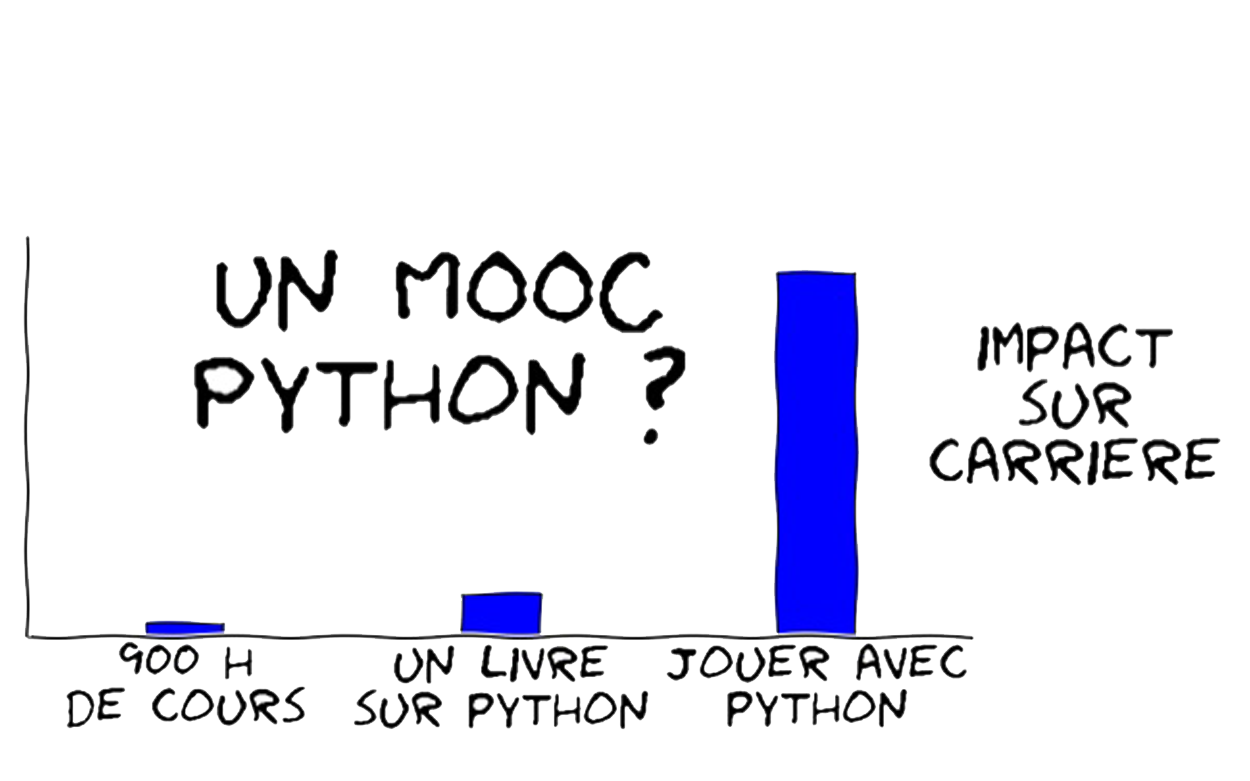
\includegraphics{medias/mooc2.png}\\
\vskip100pt

\includegraphics{medias/mooc.png}\\
\large https://www.fun-mooc.fr\\[0.5cm] % Minor heading
\large Licence CC BY-NC-ND Thierry Parmentelat et Arnaud Legout\\[0.5cm] % Minor heading

%----------------------------------------------------------------------------------------
%	DATE SECTION
%----------------------------------------------------------------------------------------

%{\large \today}\\[2cm] % Date, change the \today to a set date if you want to be precise

%----------------------------------------------------------------------------------------
%	LOGO SECTION
%----------------------------------------------------------------------------------------

%
\includegraphics{medias/logo.png}\\[1cm] 
 
%----------------------------------------------------------------------------------------

\vfill % Fill the rest of the page with whitespace

\end{titlepage}

\pagestyle{empty}
\addtocontents{toc}{\protect\thispagestyle{empty}}
\tableofcontents
\thispagestyle{empty}   



    \chapter{Introduction au MOOC et aux outils Python}
    \pagestyle{plain}
    \setcounter{page}{1}    
	    
    
    
    

    

    \hypertarget{versions-de-python}{%
\section{Versions de Python}\label{versions-de-python}}

    \hypertarget{version-de-ruxe9fuxe9rence-python-3.6}{%
\subsubsection{Version de référence~:
Python-3.6}\label{version-de-ruxe9fuxe9rence-python-3.6}}

    Comme on l'indique dans la vidéo, la version de Python qui a servi de
\textbf{référence pour le MOOC est la version 3.6}, c'est notamment avec
cette version que l'on a tourné les vidéos.

    \hypertarget{versions-plus-anciennes}{%
\subsubsection{Versions plus anciennes}\label{versions-plus-anciennes}}

    Certaines précautions sont à prendre si vous utilisez une version plus
ancienne~:

    \hypertarget{python-3.5}{%
\subparagraph{Python-3.5}\label{python-3.5}}

    Si vous préférez utiliser python-3.5, la différence la plus visible pour
vous apparaitra avec les \emph{f-strings}~:

    \begin{Verbatim}[commandchars=\\\{\},frame=single,framerule=0.3mm,rulecolor=\color{cellframecolor}]
{\color{incolor}In [{\color{incolor}1}]:} \PY{n}{age} \PY{o}{=} \PY{l+m+mi}{10}
        
        \PY{c+c1}{\PYZsh{} un exemple de f\PYZhy{}string}
        \PY{n}{f}\PY{l+s+s2}{\PYZdq{}}\PY{l+s+s2}{Jean a }\PY{l+s+si}{\PYZob{}age\PYZcb{}}\PY{l+s+s2}{ ans}\PY{l+s+s2}{\PYZdq{}}
\end{Verbatim}


\begin{Verbatim}[commandchars=\\\{\},frame=single,framerule=0.3mm,rulecolor=\color{cellframecolor}]
{\color{outcolor}Out[{\color{outcolor}1}]:} 'Jean a 10 ans'
\end{Verbatim}
            
    Cette construction - que nous utilisons très fréquemment - n'a été
introduite qu'en Python-3.6, aussi si vous utilisez Python-3.5 vous
verrez ceci~:

\begin{Shaded}
\begin{Highlighting}[frame=lines,framerule=0.6mm,rulecolor=\color{asisframecolor}]
\OperatorTok{>>>}\NormalTok{ age }\OperatorTok{=} \DecValTok{10}
\OperatorTok{>>>} \SpecialStringTok{f"Jean a }\SpecialCharTok{\{}\NormalTok{age}\SpecialCharTok{\}}\SpecialStringTok{ ans"}
\NormalTok{  File }\StringTok{"<stdin>"}\NormalTok{, line }\DecValTok{1}
    \SpecialStringTok{f"Jean a }\SpecialCharTok{\{}\NormalTok{age}\SpecialCharTok{\}}\SpecialStringTok{ ans"}
                      \OperatorTok{^}
\PreprocessorTok{SyntaxError}\NormalTok{: invalid syntax}
\end{Highlighting}
\end{Shaded}

    Dans ce cas vous devrez remplacer ce code avec la méthode
\texttt{format} - que nous verrons en Semaine 2 avec les chaines de
caractères - et dans le cas présent il faudrait remplacer par ceci~:

    \begin{Verbatim}[commandchars=\\\{\},frame=single,framerule=0.3mm,rulecolor=\color{cellframecolor}]
{\color{incolor}In [{\color{incolor}2}]:} \PY{n}{age} \PY{o}{=} \PY{l+m+mi}{10}
        
        \PY{l+s+s2}{\PYZdq{}}\PY{l+s+s2}{Jean a }\PY{l+s+si}{\PYZob{}\PYZcb{}}\PY{l+s+s2}{ ans}\PY{l+s+s2}{\PYZdq{}}\PY{o}{.}\PY{n}{format}\PY{p}{(}\PY{n}{age}\PY{p}{)}
\end{Verbatim}


\begin{Verbatim}[commandchars=\\\{\},frame=single,framerule=0.3mm,rulecolor=\color{cellframecolor}]
{\color{outcolor}Out[{\color{outcolor}2}]:} 'Jean a 10 ans'
\end{Verbatim}
            
    Comme ces f-strings sont très présents dans le cours, il est recommandé
d'utiliser au moins python-3.6.

    \hypertarget{python-3.4}{%
\subparagraph{Python-3.4}\label{python-3.4}}

    La remarque vaut donc \emph{a fortiori} pour python-3.4 qui, en outre,
ne vous permettra pas de suivre la semaine 8 sur la programmation
asynchrone, car les mots-clés \texttt{async} et \texttt{await} ont été
introduits seulement dans Python-3.5.

    \hypertarget{version-utilisuxe9e-dans-les-notebooks-versions-plus-ruxe9centes}{%
\subsubsection{Version utilisée dans les notebooks / versions plus
récentes}\label{version-utilisuxe9e-dans-les-notebooks-versions-plus-ruxe9centes}}

    Tout le cours doit pouvoir s'exécuter tel quel avec une version plus
récente de Python.

Cela dit, certains compléments illustrent des nouveautés apparues après
la 3.6, comme les \emph{dataclasses} qui sont apparues avec python-3.7,
et que nous verrons en semaine 6.

Dans tous les cas, nous \textbf{signalons systématiquement} les
notebooks qui nécessitent une version plus récente que 3.6.

    Voici enfin, à toutes fins utiles, un premier fragment de code Python
qui affiche la version de Python utilisée dans tous les notebooks de ce
cours.

Nous reviendrons en détail sur l'utilisation des notebooks dans une
prochaine séquence, dans l'immédiat pour exécuter ce code vous pouvez~:

\begin{itemize}
\tightlist
\item
  désigner avec la souris la cellule de code~; vous verrez alors
  apparaître une petite flèche à côté du mot \texttt{In}, en cliquant
  cette flèche vous exécutez le code~;
\item
  une autre méthode consiste à sélectionner la cellule de code avec la
  souris~; une fois que c'est fait vous pouvez cliquer sur le bouton
  \texttt{\textgreater{}\textbar{}\ Run} dans la barre de menu (bleue
  claire) du notebook.
\end{itemize}

    \begin{Verbatim}[commandchars=\\\{\},frame=single,framerule=0.3mm,rulecolor=\color{cellframecolor}]
{\color{incolor}In [{\color{incolor}3}]:} \PY{c+c1}{\PYZsh{} ce premier fragment de code affiche des détails sur la}
        \PY{c+c1}{\PYZsh{} version de python qui exécute tous les notebooks du cours}
        \PY{k+kn}{import} \PY{n+nn}{sys}
        \PY{n+nb}{print}\PY{p}{(}\PY{n}{sys}\PY{o}{.}\PY{n}{version\PYZus{}info}\PY{p}{)}
\end{Verbatim}


    \begin{Verbatim}[commandchars=\\\{\},frame=single,framerule=0.3mm,rulecolor=\color{cellframecolor}]
sys.version\_info(major=3, minor=7, micro=0, releaselevel='final', serial=0)
\end{Verbatim}

    Pas de panique si vous n'y arrivez pas, nous consacrerons très bientôt
une séquence entière à l'utilisation des notebooks :)


    % Add a bibliography block to the postdoc
    
    
    

        
    
    
    

    

    \hypertarget{installer-la-distribution-standard-python}{%
\section{Installer la distribution standard
Python}\label{installer-la-distribution-standard-python}}

    \hypertarget{compluxe9ment---niveau-basique}{%
\subsection{Complément - niveau
basique}\label{compluxe9ment---niveau-basique}}

    Ce complément a pour but de vous donner quelques guides pour
l'installation de la distribution standard Python 3.

Notez bien qu'il ne s'agit ici que d'indications, il existe de
nombreuses façons de procéder.

En cas de souci, commencez par chercher par vous-même, sur Google ou
autre, une solution à votre problème~; pensez également à utiliser le
forum du cours.

    Le point important est de \textbf{bien vérifier le numéro de version} de
votre installation qui doit être \textbf{au moins 3.6}

    \hypertarget{sachez-uxe0-qui-vous-parlez}{%
\subsection{Sachez à qui vous
parlez}\label{sachez-uxe0-qui-vous-parlez}}

    Mais avant qu'on n'avance sur l'installation proprement dite, il nous
faut insister sur un point qui déroute parfois les débutants. On a
parfois besoin de recourir à l'emploi d'un terminal, surtout justement
pendant la phase d'installation.

Lorsque c'est le cas, il est important de bien distinguer~:

\begin{itemize}
\tightlist
\item
  les cas où on s'adresse \textbf{au terminal} (en jargon, on dit le
  \emph{shell}),
\item
  et les cas où on s'adresse à \textbf{l'interpréteur Python}.
\end{itemize}

C'est très important car ces deux programmes ne parlent \textbf{pas} du
tout le \textbf{même langage} ! Il peut arriver au début qu'on écrive
une commande juste, mais au mauvais interlocuteur, et cela peut être
source de frustration. Essayons de bien comprendre ce point.

    \hypertarget{le-terminal}{%
\subsubsection{Le terminal}\label{le-terminal}}

Je peux dire que je parle à mon \textbf{terminal} quand l'invite de
commande (en jargon on dit le \emph{prompt}) \textbf{se termine par un
dollar \texttt{\$}} - ou un simple chevron \texttt{\textgreater{}} sur
Windows

Par exemple~sur un mac :

\begin{Shaded}
\begin{Highlighting}[frame=lines,framerule=0.6mm,rulecolor=\color{asisframecolor}]
\ExtensionTok{~/git/flotpython/w1}\NormalTok{ $ }
\end{Highlighting}
\end{Shaded}

Ou sur Windows~:

\begin{Shaded}
\begin{Highlighting}[frame=lines,framerule=0.6mm,rulecolor=\color{asisframecolor}]
\ExtensionTok{C}\NormalTok{:\textbackslash{}Users}\OperatorTok{>}
\end{Highlighting}
\end{Shaded}

    \hypertarget{linterpruxe8te-python}{%
\subsubsection{L'interprète Python}\label{linterpruxe8te-python}}

À partir du terminal, je peux lancer un \textbf{interpréteur Python},
qui se reconnaît car son prompt est fait de \textbf{3 chevrons
\texttt{\textgreater{}\textgreater{}\textgreater{}}}

\begin{Shaded}
\begin{Highlighting}[frame=lines,framerule=0.6mm,rulecolor=\color{asisframecolor}]
\ExtensionTok{~/git/flotpython/w1}\NormalTok{ $ python3}
\ExtensionTok{Python}\NormalTok{ 3.7.0 (default, Jun 29 2018, 20:14:27)}
\NormalTok{[}\ExtensionTok{Clang}\NormalTok{ 9.0.0 (clang-900.0.39.2)] }\ExtensionTok{on}\NormalTok{ darwin}
\ExtensionTok{Type} \StringTok{"help"}\NormalTok{, }\StringTok{"copyright"}\NormalTok{, }\StringTok{"credits"}\NormalTok{ or }\StringTok{"license"}\NormalTok{ for more information.}
\OperatorTok{>>>}
\end{Highlighting}
\end{Shaded}

    Pour sortir de l'interpréteur Python, et retourner au terminal,
j'utilise la fonction Python \texttt{exit()}~:

\begin{Shaded}
\begin{Highlighting}[frame=lines,framerule=0.6mm,rulecolor=\color{asisframecolor}]
\ExtensionTok{~/git/flotpython/w1}\NormalTok{ $ python3}
\OperatorTok{>>>} \ExtensionTok{20}\NormalTok{ * 60}
\ExtensionTok{1200}
\OperatorTok{>>>} \FunctionTok{exit()}
\ExtensionTok{~/git/flotpython/w1}\NormalTok{ $ python3}
\end{Highlighting}
\end{Shaded}

    \hypertarget{les-erreurs-typiques}{%
\subsubsection{Les erreurs typiques}\label{les-erreurs-typiques}}

Gardez bien cette distinction présente à l'esprit, lorsque vous lisez la
suite. Voici quelques symptômes habituels de ce qu'on obtient si on se
trompe.

Par exemple, la commande \texttt{python3\ -V} est une commande qui
s'adresse au terminal~; c'est pourquoi nous la faisons précéder d'un
dollar \texttt{\$}.

Si vous essayez de la taper alors que vous êtes déjà dans un
interpréteur python - ou sous IDLE d'ailleurs -, vous obtenez un message
d'erreur de ce genre :

\begin{Shaded}
\begin{Highlighting}[frame=lines,framerule=0.6mm,rulecolor=\color{asisframecolor}]
\OperatorTok{>>>} \ExtensionTok{python3}\NormalTok{ -V}
\ExtensionTok{Traceback}\NormalTok{ (most recent call last)}\BuiltInTok{:}
  \ExtensionTok{File} \StringTok{"<stdin>"}\NormalTok{, line 1, in }\OperatorTok{<}\NormalTok{module}\OperatorTok{>}
\ExtensionTok{NameError}\NormalTok{: name }\StringTok{'python3'}\NormalTok{ is not defined}
\end{Highlighting}
\end{Shaded}

    Réciproquement, si vous essayez de taper du Python directement dans un
terminal, ça se passe mal aussi, forcément. Par exemple sur Mac, avec
des fragments Python tout simples~:

\begin{Shaded}
\begin{Highlighting}[frame=lines,framerule=0.6mm,rulecolor=\color{asisframecolor}]
\ExtensionTok{~/git/flotpython/w1}\NormalTok{ $ import math}
\ExtensionTok{-bash}\NormalTok{: import: command not found}
\ExtensionTok{~/git/flotpython/w1}\NormalTok{ $ 30 * 60}
\ExtensionTok{-bash}\NormalTok{: 30: command not found}
\ExtensionTok{~/git/flotpython/w1}\NormalTok{ $ foo = 30 * 60}
\ExtensionTok{-bash}\NormalTok{: foo: command not found}
\end{Highlighting}
\end{Shaded}

    \hypertarget{digression---coexistence-de-python2-et-python3}{%
\subsection{Digression - coexistence de Python2 et
Python3}\label{digression---coexistence-de-python2-et-python3}}

    Avant l'arrivée de la version 3 de Python, les choses étaient simples,
on exécutait un programme Python avec une seule commande
\texttt{python}. Depuis 2014-2015, maintenant que les deux versions de
Python coexistent, il est nécessaire d'adopter une convention qui
permette d'installer les deux langages sous des noms qui sont
non-ambigus.

C'est pourquoi actuellement, on trouve \textbf{le plus souvent} la
convention suivante sous Linux et macOS~:

\begin{itemize}
\item
  \texttt{python3} est pour exécuter les programmes en Python-3~; du
  coup on trouve alors également les commandes comme \texttt{idle3} pour
  lancer IDLE, et par exemple \texttt{pip3} pour le gestionnaire de
  paquets (voir ci-dessous)~;
\item
  \texttt{python2} est pour exécuter les programmes en Python-2, avec
  typiquement \texttt{idle2} et \texttt{pip2}~;
\item
  enfin selon les systèmes, la commande \texttt{python} tout court est
  un alias pour \texttt{python2} ou \texttt{python3}. De plus en plus
  souvent, par défaut \texttt{python} désigne \texttt{python3}.
\end{itemize}

à titre d'illustration, voici ce que j'obtiens sur mon mac~:

\begin{Shaded}
\begin{Highlighting}[frame=lines,framerule=0.6mm,rulecolor=\color{asisframecolor}]
\NormalTok{$ }\ExtensionTok{python3}\NormalTok{ -V}
\ExtensionTok{Python}\NormalTok{ 3.6.2}
\NormalTok{$ }\ExtensionTok{python2}\NormalTok{ -V}
\ExtensionTok{Python}\NormalTok{ 2.7.13}
\NormalTok{$ }\ExtensionTok{python}\NormalTok{ -V}
\ExtensionTok{Python}\NormalTok{ 3.6.2}
\end{Highlighting}
\end{Shaded}

Sous Windows, vous avez un lanceur qui s'appelle \texttt{py}. Par
défaut, il lance la version de Python la plus récente installée, mais
vous pouvez spécifier une version spécifique de la manière suivante~:

\begin{Shaded}
\begin{Highlighting}[frame=lines,framerule=0.6mm,rulecolor=\color{asisframecolor}]
\ExtensionTok{C}\NormalTok{:}\DataTypeTok{\textbackslash{}>}\NormalTok{ py -2.7}
\end{Highlighting}
\end{Shaded}

pour lancer, par exemple, Python en version 2.7. Vous trouverez toute la
documentation nécessaire pour Windows sur cette page (en anglais)~:
https://docs.python.org/3/using/windows.html

Pour éviter d'éventuelles confusions, nous précisons toujours
\texttt{python3} dans le cours.

    \hypertarget{installation-de-base}{%
\subsection{Installation de base}\label{installation-de-base}}

    \hypertarget{vous-utilisez-windows}{%
\subsubsection{Vous utilisez Windows}\label{vous-utilisez-windows}}

    La méthode recommandée sur Windows est de partir de la page
https://www.python.org/download où vous trouverez un programme
d'installation qui contient tout ce dont vous aurez besoin pour suivre
le cours.

Pour vérifier que vous êtes prêt, il vous faut lancer IDLE (quelque part
dans le menu Démarrer) et vérifier le numéro de version.

    \hypertarget{vous-utilisez-macos}{%
\subsubsection{Vous utilisez macOS}\label{vous-utilisez-macos}}

    Ici encore, la méthode recommandée est de partir de la page
https://www.python.org/download et d'utiliser le programme
d'installation.

Sachez aussi, si vous utilisez déjà MacPorts (https://www.macports.org),
que vous pouvez également utiliser cet outil pour installer, par exemple
Python 3.6, avec la commande

    \begin{Shaded}
\begin{Highlighting}[frame=lines,framerule=0.6mm,rulecolor=\color{asisframecolor}]
\NormalTok{$ }\FunctionTok{sudo}\NormalTok{ port install python36}
\end{Highlighting}
\end{Shaded}

    \hypertarget{vous-utilisez-linux}{%
\subsubsection{Vous utilisez Linux}\label{vous-utilisez-linux}}

    Dans ce cas il est très probable que Python-3.x soit déjà disponible sur
votre machine. Pour vous en assurer, essayez de lancer la commande
\texttt{python3} dans un terminal.

    \hypertarget{rhel-fedora}{%
\subparagraph{RHEL / Fedora}\label{rhel-fedora}}

    Voici par exemple ce qu'on obtient depuis un terminal sur une machine
installée en Fedora-20~:

    \begin{Shaded}
\begin{Highlighting}[frame=lines,framerule=0.6mm,rulecolor=\color{asisframecolor}]
\NormalTok{$ }\ExtensionTok{python3}
\ExtensionTok{Python}\NormalTok{ 3.6.2 (default, Jul 20 2017, 12:30:02)}
\NormalTok{[}\ExtensionTok{GCC}\NormalTok{ 6.3.1 20161221 (Red Hat 6.3.1-1)] }\ExtensionTok{on}\NormalTok{ linux}
\ExtensionTok{Type} \StringTok{"help"}\NormalTok{, }\StringTok{"copyright"}\NormalTok{, }\StringTok{"credits"}\NormalTok{ or }\StringTok{"license"}\NormalTok{ for more information.}
\OperatorTok{>>>} \FunctionTok{exit()}
\end{Highlighting}
\end{Shaded}

    \textbf{Vérifiez bien le numéro de version} qui doit être en 3.\emph{x}.
Si vous obtenez un message du style
\texttt{python3:\ command\ not\ found} utilisez \texttt{dnf}
(anciennement connu sous le nom de \texttt{yum}) pour installer le rpm
\texttt{python3} comme ceci~:

    \begin{Shaded}
\begin{Highlighting}[frame=lines,framerule=0.6mm,rulecolor=\color{asisframecolor}]
\NormalTok{$ }\FunctionTok{sudo}\NormalTok{ dnf install python3}
\end{Highlighting}
\end{Shaded}

    S'agissant d'\texttt{idle}, l'éditeur que nous utilisons dans le cours
(optionnel si vous êtes familier avec un éditeur de texte), vérifiez sa
présence comme ceci~:

    \begin{Shaded}
\begin{Highlighting}[frame=lines,framerule=0.6mm,rulecolor=\color{asisframecolor}]
\NormalTok{$ }\BuiltInTok{type}\NormalTok{ idle3}
\ExtensionTok{idle}\NormalTok{ is hashed (/usr/bin/idle3)}
\end{Highlighting}
\end{Shaded}

    Ici encore, si la commande n'est pas disponible vous pouvez l'installer
avec~:

    \begin{Shaded}
\begin{Highlighting}[frame=lines,framerule=0.6mm,rulecolor=\color{asisframecolor}]
\NormalTok{$ }\FunctionTok{sudo}\NormalTok{ yum install python3-tools}
\end{Highlighting}
\end{Shaded}

    \hypertarget{debian-ubuntu}{%
\subparagraph{Debian / Ubuntu}\label{debian-ubuntu}}

    Ici encore, Python-2.7 est sans doute déjà disponible. Procédez comme
ci-dessus, voici un exemple recueilli dans un terminal sur une machine
installée en Ubuntu-14.04/trusty~:

    \begin{Shaded}
\begin{Highlighting}[frame=lines,framerule=0.6mm,rulecolor=\color{asisframecolor}]
\NormalTok{$ }\ExtensionTok{python3}
\ExtensionTok{Python}\NormalTok{ 3.6.2 (default, Jul 20 2017, 12:30:02)}
\NormalTok{[}\ExtensionTok{GCC}\NormalTok{ 6.3.1 20161221 (Red Hat 6.3.1-1)] }\ExtensionTok{on}\NormalTok{ linux}
\ExtensionTok{Type} \StringTok{"help"}\NormalTok{, }\StringTok{"copyright"}\NormalTok{, }\StringTok{"credits"}\NormalTok{ or }\StringTok{"license"}\NormalTok{ for more information.}
\OperatorTok{>>>} \FunctionTok{exit()}
\end{Highlighting}
\end{Shaded}

    Pour installer Python~:

    \begin{Shaded}
\begin{Highlighting}[frame=lines,framerule=0.6mm,rulecolor=\color{asisframecolor}]
\NormalTok{$ }\FunctionTok{sudo}\NormalTok{ apt-get install python3}
\end{Highlighting}
\end{Shaded}

    Pour installer idle~:

    \begin{Shaded}
\begin{Highlighting}[frame=lines,framerule=0.6mm,rulecolor=\color{asisframecolor}]
\NormalTok{$ }\FunctionTok{sudo}\NormalTok{ apt-get install idle3}
\end{Highlighting}
\end{Shaded}

    \hypertarget{installation-de-bibliothuxe8ques-compluxe9mentaires}{%
\subsubsection{Installation de bibliothèques
complémentaires}\label{installation-de-bibliothuxe8ques-compluxe9mentaires}}

    Il existe un outil très pratique pour installer des bibliothèques
Python, il s'appelle \texttt{pip3}, qui est documenté ici
https://pypi.python.org/pypi/pip

    Sachez aussi, si par ailleurs vous utilisez un gestionnaire de paquets
comme \texttt{rpm} sur RHEL, \texttt{apt-get} sur Debian, ou
\texttt{port} sur macOS, que de nombreux paquets sont également
disponibles au travers de ces outils.

    \hypertarget{anaconda}{%
\subsubsection{Anaconda}\label{anaconda}}

    Sachez qu'il existe beaucoup de distributions alternatives qui incluent
Python~; parmi elles, la plus populaire est sans aucun doute
\href{https://www.anaconda.com/}{Anaconda}, qui contient un grand nombre
de bibliothèques de calcul scientifique, et également d'ailleurs Jupyter
pour travailler nativement sur des notebooks au format \texttt{.ipynb}.

Anaconda vient avec son propre gestionnaire de paquets pour
l'installation de bibliothèques supplémentaires qui s'appelle
\texttt{conda}.


    % Add a bibliography block to the postdoc
    
    
    

        
    
    
    

    

    \hypertarget{un-peu-de-lecture}{%
\section{Un peu de lecture}\label{un-peu-de-lecture}}

    \hypertarget{compluxe9ment---niveau-basique}{%
\subsection{Complément - niveau
basique}\label{compluxe9ment---niveau-basique}}

    \hypertarget{mise-uxe0-jour-de-juillet-2018}{%
\subsubsection{Mise à jour de Juillet
2018}\label{mise-uxe0-jour-de-juillet-2018}}

    Le 12 Juillet 2018, Guido van Rossum
\href{https://lwn.net/Articles/759654/}{a annoncé qu'il quittait la
fonction de BDFL} qu'il occupait depuis près de trois décennies. Il
n'est pas tout à fait clair à ce stade comment va évoluer la gouvernance
de Python.

    \hypertarget{le-zen-de-python}{%
\subsubsection{Le Zen de Python}\label{le-zen-de-python}}

    Vous pouvez lire le ``Zen de Python'', qui résume la philosophie du
langage, en important le module \texttt{this} avec ce code~: (pour
exécuter ce code, cliquez dans la cellule de code, et faites au clavier
``Majuscule/Entrée'' ou ``Shift/Enter'')

    \begin{Verbatim}[commandchars=\\\{\},frame=single,framerule=0.3mm,rulecolor=\color{cellframecolor}]
{\color{incolor}In [{\color{incolor}1}]:} \PY{c+c1}{\PYZsh{} le Zen de Python}
        \PY{k+kn}{import} \PY{n+nn}{this}
\end{Verbatim}


    \begin{Verbatim}[commandchars=\\\{\},frame=single,framerule=0.3mm,rulecolor=\color{cellframecolor}]
The Zen of Python, by Tim Peters

Beautiful is better than ugly.
Explicit is better than implicit.
Simple is better than complex.
Complex is better than complicated.
Flat is better than nested.
Sparse is better than dense.
Readability counts.
Special cases aren't special enough to break the rules.
Although practicality beats purity.
Errors should never pass silently.
Unless explicitly silenced.
In the face of ambiguity, refuse the temptation to guess.
There should be one-- and preferably only one --obvious way to do it.
Although that way may not be obvious at first unless you're Dutch.
Now is better than never.
Although never is often better than *right* now.
If the implementation is hard to explain, it's a bad idea.
If the implementation is easy to explain, it may be a good idea.
Namespaces are one honking great idea -- let's do more of those!
\end{Verbatim}

    \hypertarget{documentation}{%
\subsubsection{Documentation}\label{documentation}}

    \begin{itemize}
\item
  On peut commencer par citer
  l'\href{http://fr.wikipedia.org/wiki/Python_\%28langage\%29}{article
  de Wikipédia sur Python en français}.
\item
  La \href{https://wiki.python.org/moin/FrenchLanguage}{page sur le
  langage en français}.
\item
  La \href{https://docs.python.org/3/}{documentation originale} de
  Python 3 - donc, en anglais - est un très bon point d'entrée lorsqu'on
  cherche un sujet particulier, mais (beaucoup) trop abondante pour être
  lue d'un seul trait. Pour chercher de la documentation sur un module
  particulier, le plus simple est encore d'utiliser Google - ou votre
  moteur de recherche favori - qui vous redirigera, dans la grande
  majorité des cas, vers la page qui va bien dans, précisément, la
  documentation de Python.

  À titre d'exercice, cherchez la documentation du module
  \texttt{pathlib} en
  \href{https://www.google.fr/search?q=python+module+pathlib}{cherchant
  sur Google} les mots-clé \texttt{"python\ module\ pathlib"}.
\item
  J'aimerais vous signaler également une initiative pour
  \href{https://docs.python.org/fr/3/}{traduire la documentation
  officielle en français}.
\end{itemize}

    \hypertarget{historique-et-survol}{%
\subsubsection{Historique et survol}\label{historique-et-survol}}

    \begin{itemize}
\tightlist
\item
  La FAQ officielle de Python (en anglais) sur
  \href{https://docs.python.org/3/faq/design.html}{les choix de
  conception et l'historique du langage}.
\item
  L'article de Wikipédia (en anglais) sur
  l'\href{http://en.wikipedia.org/wiki/History_of_Python}{historique du
  langage}.
\item
  Sur Wikipédia, un article (en anglais) sur
  \href{http://en.wikipedia.org/wiki/Python_syntax_and_semantics}{la
  syntaxe et la sémantique de Python}.
\end{itemize}

    \hypertarget{un-peu-de-folklore}{%
\subsubsection{Un peu de folklore}\label{un-peu-de-folklore}}

    \begin{itemize}
\tightlist
\item
  Le \href{https://www.youtube.com/watch?v=YgtL4S7Hrwo}{discours de
  Guido van Rossum à PyCon 2016}.
\item
  Sur YouTube, le
  \href{https://www.youtube.com/watch?v=anwy2MPT5RE}{sketch des Monty
  Python} d'où proviennent les termes \texttt{spam}, \texttt{eggs} et
  autres \texttt{beans} que l'on utilise traditionnellement dans les
  exemples en Python plutôt que \texttt{foo} et \texttt{bar}.
\item
  L'\href{http://en.wikipedia.org/wiki/Spam_\%28Monty_Python\%29}{article
  Wikipédia correspondant}, qui cite le langage Python.
\end{itemize}

    \hypertarget{compluxe9ment---niveau-intermuxe9diaire}{%
\subsection{Complément - niveau
intermédiaire}\label{compluxe9ment---niveau-intermuxe9diaire}}

    \hypertarget{licence}{%
\subsubsection{Licence}\label{licence}}

    \begin{itemize}
\tightlist
\item
  La \href{https://docs.python.org/3/license.html}{licence d'utilisation
  est disponible ici}.
\item
  La page de la \href{https://www.python.org/psf/}{Python Software
  Foundation}, qui est une entité légale similaire à nos associations de
  1901, à but non lucratif~; elle possède les droits sur le langage.
\end{itemize}

    \hypertarget{le-processus-de-duxe9veloppement}{%
\subsubsection{Le processus de
développement}\label{le-processus-de-duxe9veloppement}}

    \begin{itemize}
\tightlist
\item
  Comment les choix d'évolution sont proposés et discutés,
  \href{http://en.wikipedia.org/wiki/Python_\%28programming_language\%29\#Development}{au
  travers des PEP (Python Enhancement Proposals) - sur wikipedia}
\item
  \href{http://legacy.python.org/dev/peps/pep-0001/}{Le premier PEP:
  PEP-001 donc} décrit en détail le cycle de vie des PEPs
\item
  Le \href{http://legacy.python.org/dev/peps/pep-0008}{PEP 008}, qui
  préconise un style de présentation (\emph{style guide})
\item
  L'\href{http://legacy.python.org/dev/peps/}{index de tous les PEPs}
\end{itemize}


    % Add a bibliography block to the postdoc
    
    
    

        \hypertarget{notebooks-jupyter-comme-support-de-cours}{%
\section{``Notebooks'' Jupyter comme support de
cours}\label{notebooks-jupyter-comme-support-de-cours}}

    Pour illustrer les vidéos du MOOC, nous avons choisi d'utiliser Jupyter
pour vous rédiger les documents ``mixtes'' contenant du texte et du code
Python, qu'on appelle des ``notebooks'', et dont le présent document est
un exemple.

Nous allons, dans la suite, utiliser du code Python, pourtant nous
n'avons pas encore abordé le langage. Pas d'inquiétude, ce code est
uniquement destiné à valider le fonctionnement des notebooks, et nous
n'utilisons que des choses très simples.

    \hypertarget{avertissement-ruxe9glages-du-navigateur}{%
\subsubsection{Avertissement: réglages du
navigateur}\label{avertissement-ruxe9glages-du-navigateur}}

    Avant toute chose, pour un bon fonctionnement des notebooks, on rappelle
qu'il est nécessaire d'avoir \textbf{autorisé} dans votre navigateur les
\textbf{cookies} en provenance du site Internet
\textbf{\texttt{nbhosting.inria.fr}}, qui héberge l'infrastructure qui
héberge tous les notebooks.

    \hypertarget{avantages-des-notebooks}{%
\subsubsection{Avantages des notebooks}\label{avantages-des-notebooks}}

    Comme vous le voyez, ce support permet un format plus lisible que des
commentaires dans un fichier de code.

    Nous attirons votre attention sur le fait que \textbf{les fragments de
code peuvent être évalués et modifiés}. Ainsi vous pouvez facilement
essayer des variantes autour du notebook original.

Notez bien également que le code Python est interprété \textbf{sur une
machine distante}, ce qui vous permet de faire vos premiers pas avant
même d'avoir procédé à l'installation de Python sur votre propre
ordinateur.

    \hypertarget{comment-utiliser-les-notebooks}{%
\subsubsection{Comment utiliser les
notebooks}\label{comment-utiliser-les-notebooks}}

    En haut du notebook, vous avez une barre de menu (sur fond bleu clair),
contenant~:

\begin{itemize}
	\item
un titre pour le notebook, avec un numéro de version~;
	\item
une barre de menus avec les entrées \texttt{File}, \texttt{Insert},
\texttt{Cell}, \texttt{Kernel};
	\item
et une barre de boutons qui sont des
raccourcis vers certains menus fréquemment utilisés. Si vous laissez
votre souris au dessus d'un bouton, un petit texte apparaît, indiquant à
quelle fonction correspond ce bouton.
\end{itemize}

Nous avons vu dans la vidéo qu'un notebook est constitué d'une suite de
cellules, soit textuelles, soit contenant du code. Les cellules de code
sont facilement reconnaissables, elles sont précédées de
\texttt{In\ {[}\ {]}:}. La cellule qui suit celle que vous êtes en train
de lire est une cellule de code.

Pour commencer, sélectionnez cette cellule de code avec votre souris, et
appuyez dans la barre de menu - en haut du notebook, donc - sur celui en
forme de flèche triangulaire vers la droite (Play)~: 

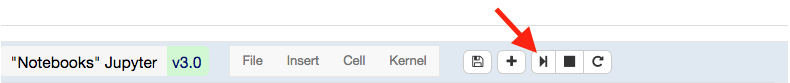
\includegraphics{medias/notebook-eval-button.png}\\
    \begin{Verbatim}[commandchars=\\\{\}]
{\color{incolor}In [{\color{incolor}1}]:} \PY{l+m+mi}{20} \PY{o}{*} \PY{l+m+mi}{30}
\end{Verbatim}


\begin{Verbatim}[commandchars=\\\{\}]
{\color{outcolor}Out[{\color{outcolor}1}]:} 600
\end{Verbatim}
            
    Comme vous le voyez, la cellule est ``exécutée'' (on dira plus
volontiers évaluée), et on passe à la cellule suivante.

Alternativement, vous pouvez simplement taper au clavier
\textbf{\emph{Shift+Enter}}, ou selon les claviers
\textbf{\emph{Maj-Entrée}}, pour obtenir le même effet. D'une manière
générale, il est important d'apprendre et d'utiliser les raccourcis
clavier, cela vous fera gagner beaucoup de temps par la suite.

    La façon habituelle d'\emph{exécuter} l'ensemble du notebook consiste~:
\begin{itemize}
	\item
	à sélectionner la première cellule,
	\item
	et à taper \textbf{\emph{Shift+Enter}} jusqu'à attendre la fin du notebook.
\end{itemize}

    Lorsqu'une cellule de code a été évaluée, Jupyter ajoute sous la cellule
\texttt{In} une cellule \texttt{Out} qui donne le résultat du fragment
Python, soit ci-dessus 600.\\

Jupyter ajoute également un nombre entre les crochets pour afficher, par
exemple ci-dessus, \texttt{In\ {[}1{]}:}. Ce nombre vous permet de
retrouver l'ordre dans lequel les cellules ont été évaluées.

    Vous pouvez naturellement modifier ces cellules de code pour faire des
essais~; ainsi vous pouvez vous servir du modèle ci-dessous pour
calculer la racine carrée de 3, ou essayer la fonction sur un nombre
négatif et voir comment est signalée l'erreur.

    \begin{Verbatim}[commandchars=\\\{\}]
{\color{incolor}In [{\color{incolor}2}]:} \PY{c+c1}{\PYZsh{} math.sqrt (pour square root) calcule la racine carrée}
        \PY{k+kn}{import} \PY{n+nn}{math}
        \PY{n}{math}\PY{o}{.}\PY{n}{sqrt}\PY{p}{(}\PY{l+m+mi}{2}\PY{p}{)}
\end{Verbatim}


\begin{Verbatim}[commandchars=\\\{\}]
{\color{outcolor}Out[{\color{outcolor}2}]:} 1.4142135623730951
\end{Verbatim}
            
    On peut également évaluer tout le notebook en une seule fois en
utilisant le menu \emph{Cell -\textgreater{} Run All}.

    \hypertarget{attention-uxe0-bien-uxe9valuer-les-cellules-dans-lordre}{%
\subsubsection{Attention à bien évaluer les cellules dans
l'ordre}\label{attention-uxe0-bien-uxe9valuer-les-cellules-dans-lordre}}

    Il est important que les cellules de code soient évaluées dans le bon
ordre. Si vous ne respectez pas l'ordre dans lequel les cellules de code
sont présentées, le résultat peut être inattendu.\\

En fait, évaluer un programme sous forme de notebook revient à le
découper en petits fragments, et si on exécute ces fragments dans le
désordre, on obtient naturellement un programme différent.

    On le voit sur cet exemple~:

    \begin{Verbatim}[commandchars=\\\{\}]
{\color{incolor}In [{\color{incolor}3}]:} \PY{n}{message} \PY{o}{=} \PY{l+s+s2}{\PYZdq{}}\PY{l+s+s2}{Il faut faire attention à l}\PY{l+s+s2}{\PYZsq{}}\PY{l+s+s2}{ordre dans lequel on évalue les notebooks}\PY{l+s+s2}{\PYZdq{}}
\end{Verbatim}


    \begin{Verbatim}[commandchars=\\\{\}]
{\color{incolor}In [{\color{incolor}4}]:} \PY{n+nb}{print}\PY{p}{(}\PY{n}{message}\PY{p}{)}
\end{Verbatim}


    \begin{Verbatim}[commandchars=\\\{\}]
Il faut faire attention à l'ordre dans lequel on évalue les notebooks

    \end{Verbatim}

    Si un peu plus loin dans le notebook on fait par exemple~:

    \begin{Verbatim}[commandchars=\\\{\}]
{\color{incolor}In [{\color{incolor}5}]:} \PY{c+c1}{\PYZsh{} ceci a pour effet d\PYZsq{}effacer la variable \PYZsq{}message\PYZsq{}}
        \PY{k}{del} \PY{n}{message}
\end{Verbatim}


    qui rend le symbole \texttt{message} indéfini, alors bien sûr on ne peut
plus évaluer la cellule qui fait \texttt{print} puisque la variable
\texttt{message} n'est plus connue de l'interpréteur.

    \hypertarget{ruxe9initialiser-linterpruxe9teur}{%
\subsubsection{Réinitialiser
l'interpréteur}\label{ruxe9initialiser-linterpruxe9teur}}

    Si vous faites trop de modifications, ou perdez le fil de ce que vous
avez évalué, il peut être utile de redémarrer votre interpréteur. Le
menu \emph{Kernel~→~Restart} vous permet de faire cela, un peu à la
manière de IDLE qui repart d'un interpréteur vierge lorsque vous
utilisez la fonction F5.

    Le menu \emph{Kernel~→~Interrupt} peut être quant à lui utilisé si votre
fragment prend trop longtemps à s'exécuter (par exemple vous avez écrit
une boucle dont la logique est cassée et qui ne termine pas).

    \hypertarget{vous-travaillez-sur-une-copie}{%
\subsubsection{Vous travaillez sur une
copie}\label{vous-travaillez-sur-une-copie}}

    Un des avantages principaux des notebooks est de vous permettre de
modifier le code que nous avons écrit, et de voir par vous-mêmes comment
se comporte le code modifié.\\

Pour cette raison, chaque élève dispose de sa \textbf{propre copie} de
chaque notebook, vous pouvez bien sûr apporter toutes les modifications
que vous souhaitez à vos notebooks sans affecter les autres étudiants.

    \hypertarget{revenir-uxe0-la-version-du-cours}{%
\subsubsection{Revenir à la version du
cours}\label{revenir-uxe0-la-version-du-cours}}

    Vous pouvez toujours revenir à la version ``du cours'' grâce au menu
\emph{File~→~Reset to original}.\\

    Attention, avec cette fonction vous restaurez \textbf{tout le notebook}
et donc \textbf{vous perdez vos modifications sur ce notebook}.

    \hypertarget{tuxe9luxe9charger-au-format-python}{%
\subsubsection{Télécharger au format
Python}\label{tuxe9luxe9charger-au-format-python}}

    Vous pouvez télécharger un notebook au format Python sur votre
ordinateur grâce au menu \emph{File~→~Download~as~→~Python}

    Les cellules de texte sont préservées dans le résultat sous forme de
commentaires Python.

    \hypertarget{partager-un-notebook-en-lecture-seule}{%
\subsubsection{Partager un notebook en lecture
seule}\label{partager-un-notebook-en-lecture-seule}}

    Enfin, avec le menu \emph{File~→~Share~static~version}, vous pouvez
publier une version en lecture seule de votre notebook~; vous obtenez
une URL que vous pouvez publier, par exemple pour demander de l'aide sur
le forum. Ainsi, les autres étudiants peuvent accéder en lecture seule à
votre code.\\

    Notez que lorsque vous utilisez cette fonction plusieurs fois, c'est
toujours la dernière version publiée que verront vos camarades, l'URL
utilisée reste toujours la même pour un étudiant et un notebook donné.

    \hypertarget{ajouter-des-cellules}{%
\subsubsection{Ajouter des cellules}\label{ajouter-des-cellules}}

    Vous pouvez ajouter une cellule n'importe où dans le document avec le
bouton \textbf{+} de la barre de boutons.\\

Aussi, lorsque vous arrivez à la fin du document, une nouvelle cellule
est créée chaque fois que vous évaluez la dernière cellule~; de cette
façon vous disposez d'un brouillon pour vos propres essais.\\

À vous de jouer.

        
    
    
    

    

    \hypertarget{modes-dexuxe9cution}{%
\section{Modes d'exécution}\label{modes-dexuxe9cution}}

    Nous avons donc à notre disposition plusieurs façons d'exécuter un
programme Python. Nous allons les étudier plus en détail~:

    \begin{longtable}[]{@{}ll@{}}
\toprule
Quoi & Avec quel outil\tabularnewline
\midrule
\endhead
fichier complet &
\texttt{python3\ \textless{}fichier\textgreater{}.py}\tabularnewline
ligne à ligne & \texttt{python3} en mode interactif\tabularnewline
~ & ou sous \texttt{ipython3}\tabularnewline
~ & ou avec IDLE\tabularnewline
par fragments & dans un notebook\tabularnewline
\bottomrule
\end{longtable}

    Pour cela nous allons voir le comportement d'un tout petit programme
Python lorsqu'on l'exécute sous ces différents environnements.

On veut surtout expliquer une petite différence quant au niveau de
détail de ce qui se trouve imprimé.

    Essentiellement, lorsqu'on utilise l'interpréteur en mode interactif -
ou sous IDLE - à chaque fois que l'on tape une ligne, le résultat est
\textbf{calculé} (on dit aussi \textbf{évalué}) puis \textbf{imprimé}.

Par contre, lorsqu'on écrit tout un programme, on ne peut plus imprimer
le résultat de toutes les lignes, cela produirait un flot d'impression
beaucoup trop important. Par conséquent, si vous ne déclenchez pas une
impression avec, par exemple, la fonction \texttt{print}, rien ne
s'affichera.

Enfin, en ce qui concerne le notebook, le comportement est un peu
hybride entre les deux, en ce sens que seul le \textbf{dernier résultat}
de la cellule est imprimé.

    \hypertarget{linterpruxe9teur-python-interactif}{%
\subsubsection{L'interpréteur Python
interactif}\label{linterpruxe9teur-python-interactif}}

    Le programme choisi est très simple, c'est le suivant~:

    \begin{Shaded}
\begin{Highlighting}[frame=lines,framerule=0.6mm,rulecolor=\color{asisframecolor}]
\DecValTok{10} \OperatorTok{*} \DecValTok{10}
\DecValTok{20} \OperatorTok{*} \DecValTok{20}
\DecValTok{30} \OperatorTok{*} \DecValTok{30}
\end{Highlighting}
\end{Shaded}

    Voici comment se comporte l'interpréteur interactif quand on lui soumet
ces instructions~:

    \begin{Shaded}
\begin{Highlighting}[frame=lines,framerule=0.6mm,rulecolor=\color{asisframecolor}]
\NormalTok{$ python3}
\NormalTok{Python }\DecValTok{3}\NormalTok{.}\FloatTok{5.1}\NormalTok{ (v3.}\FloatTok{5.1}\NormalTok{:37a07cee5969, Dec  }\DecValTok{5} \DecValTok{2015}\NormalTok{, }\DecValTok{21}\NormalTok{:}\DecValTok{12}\NormalTok{:}\DecValTok{44}\NormalTok{)}
\NormalTok{[GCC }\DecValTok{4}\NormalTok{.}\FloatTok{2.1}\NormalTok{ (Apple Inc. build }\DecValTok{5666}\NormalTok{) (dot }\DecValTok{3}\NormalTok{)] on darwin}
\NormalTok{Type }\StringTok{"help"}\NormalTok{, }\StringTok{"copyright"}\NormalTok{, }\StringTok{"credits"} \KeywordTok{or} \StringTok{"license"} \ControlFlowTok{for}\NormalTok{ more information.}
\OperatorTok{>>>} \DecValTok{10} \OperatorTok{*} \DecValTok{10}
\DecValTok{100}
\OperatorTok{>>>} \DecValTok{20} \OperatorTok{*} \DecValTok{20}
\DecValTok{400}
\OperatorTok{>>>} \DecValTok{30} \OperatorTok{*} \DecValTok{30}
\DecValTok{900}
\OperatorTok{>>>}\NormalTok{ exit()}
\NormalTok{$}
\end{Highlighting}
\end{Shaded}

    Notez que pour terminer la session, il nous faut ``sortir'' de
l'interpréteur en tapant \texttt{exit()}.

On peut aussi taper \texttt{Control-D} sous Linux ou macOS.

    Comme on le voit ici, l'interpréteur imprime \textbf{le résultat de
chaque ligne}. On voit bien apparaître toutes les valeurs calculées,
100, 400, puis enfin 900.

    \hypertarget{sous-forme-de-programme-constituuxe9}{%
\subsubsection{Sous forme de programme
constitué}\label{sous-forme-de-programme-constituuxe9}}

    Voyons à présent ce que donne cette même séquence de calculs dans un
programme complet. Pour cela, il nous faut tout d'abord fabriquer un
fichier avec un suffixe en \texttt{.py}, en utilisant par exemple un
éditeur de fichier. Le résultat doit ressembler à ceci~:

    \begin{Shaded}
\begin{Highlighting}[frame=lines,framerule=0.6mm,rulecolor=\color{asisframecolor}]
\NormalTok{$ }\FunctionTok{cat}\NormalTok{ foo.py}
\ExtensionTok{10}\NormalTok{ * 10}
\ExtensionTok{20}\NormalTok{ * 20}
\ExtensionTok{30}\NormalTok{ * 30}
\NormalTok{$}
\end{Highlighting}
\end{Shaded}

    Exécutons à présent ce programme~:

    \begin{Shaded}
\begin{Highlighting}[frame=lines,framerule=0.6mm,rulecolor=\color{asisframecolor}]
\NormalTok{$ }\ExtensionTok{python3}\NormalTok{ foo.py}
\NormalTok{$}
\end{Highlighting}
\end{Shaded}

    On constate donc que ce programme \textbf{ne fait rien~!} En tout cas,
selon toute apparence.

En réalité, les 3 valeurs 100, 400 et 900 sont bien calculées, mais
comme aucune instruction \texttt{print} n'est présente, rien n'est
imprimé et le programme se termine sans signe apparent d'avoir
réellement fonctionné.

Ce comportement peut paraître un peu déroutant au début, mais comme nous
l'avons mentionné c'est tout à fait délibéré. Un programme fonctionnel
faisant facilement plusieurs milliers de lignes, voire beaucoup plus, il
ne serait pas du tout réaliste que chaque ligne produise une impression,
comme c'est le cas en mode interactif.

    \hypertarget{dans-un-notebook}{%
\subsubsection{Dans un notebook}\label{dans-un-notebook}}

    Voici à présent le même programme dans un notebook~:

    \begin{Verbatim}[commandchars=\\\{\},frame=single,framerule=0.3mm,rulecolor=\color{cellframecolor}]
{\color{incolor}In [{\color{incolor}1}]:} \PY{l+m+mi}{10} \PY{o}{*} \PY{l+m+mi}{10}
        \PY{l+m+mi}{20} \PY{o}{*} \PY{l+m+mi}{20}
        \PY{l+m+mi}{30} \PY{o}{*} \PY{l+m+mi}{30}
\end{Verbatim}


\begin{Verbatim}[commandchars=\\\{\},frame=single,framerule=0.3mm,rulecolor=\color{cellframecolor}]
{\color{outcolor}Out[{\color{outcolor}1}]:} 900
\end{Verbatim}
            
    Lorsqu'on exécute cette cellule (rappel~: sélectionner la cellule, et
utiliser le bouton en forme de flèche vers la droite, ou entrer
\textbf{``Shift+Enter''} au clavier), on obtient une seule valeur dans
la rubrique \texttt{Out{[}{]}}, 900, qui correspond \textbf{au résultat
de la dernière ligne.}

    \hypertarget{utiliser-print}{%
\subsubsection{\texorpdfstring{Utiliser
\texttt{print}}{Utiliser print}}\label{utiliser-print}}

    Ainsi, pour afficher un résultat intermédiaire, on utilise l'instruction
\texttt{print}. Nous verrons cette instruction en détail dans les
semaines qui viennent, mais en guise d'introduction disons seulement que
c'est une fonction comme les autres en Python 3.

    \begin{Verbatim}[commandchars=\\\{\},frame=single,framerule=0.3mm,rulecolor=\color{cellframecolor}]
{\color{incolor}In [{\color{incolor}2}]:} \PY{n}{a} \PY{o}{=} \PY{l+m+mi}{10}
        \PY{n}{b} \PY{o}{=} \PY{l+m+mi}{20}
        
        \PY{n+nb}{print}\PY{p}{(}\PY{n}{a}\PY{p}{,} \PY{n}{b}\PY{p}{)}
\end{Verbatim}


    \begin{Verbatim}[commandchars=\\\{\},frame=single,framerule=0.3mm,rulecolor=\color{cellframecolor}]
10 20
\end{Verbatim}

    On peut naturellement mélanger des objets de plusieurs types, et donc
mélanger des chaînes de caractères et des nombres pour obtenir un
résultat un peu plus lisible. En effet, lorsque le programme devient
gros, il est important de savoir à quoi correspond une ligne dans le
flot de toutes les impressions. Aussi on préfèrera quelque chose comme~:

    \begin{Verbatim}[commandchars=\\\{\},frame=single,framerule=0.3mm,rulecolor=\color{cellframecolor}]
{\color{incolor}In [{\color{incolor}3}]:} \PY{n+nb}{print}\PY{p}{(}\PY{l+s+s2}{\PYZdq{}}\PY{l+s+s2}{a =}\PY{l+s+s2}{\PYZdq{}}\PY{p}{,} \PY{n}{a}\PY{p}{,} \PY{l+s+s2}{\PYZdq{}}\PY{l+s+s2}{et b =}\PY{l+s+s2}{\PYZdq{}}\PY{p}{,} \PY{n}{b}\PY{p}{)}
\end{Verbatim}


    \begin{Verbatim}[commandchars=\\\{\},frame=single,framerule=0.3mm,rulecolor=\color{cellframecolor}]
a = 10 et b = 20
\end{Verbatim}

    \begin{Verbatim}[commandchars=\\\{\},frame=single,framerule=0.3mm,rulecolor=\color{cellframecolor}]
{\color{incolor}In [{\color{incolor}4}]:} \PY{c+c1}{\PYZsh{} ou encore, équivalente mais avec un f\PYZhy{}string}
        \PY{n+nb}{print}\PY{p}{(}\PY{n}{f}\PY{l+s+s2}{\PYZdq{}}\PY{l+s+s2}{a = }\PY{l+s+si}{\PYZob{}a\PYZcb{}}\PY{l+s+s2}{ et b = }\PY{l+s+si}{\PYZob{}b\PYZcb{}}\PY{l+s+s2}{\PYZdq{}}\PY{p}{)}
\end{Verbatim}


    \begin{Verbatim}[commandchars=\\\{\},frame=single,framerule=0.3mm,rulecolor=\color{cellframecolor}]
a = 10 et b = 20
\end{Verbatim}

    Une pratique courante consiste d'ailleurs à utiliser les commentaires
pour laisser dans le code les instructions \texttt{print} qui
correspondent à du debug (c'est-à-dire qui ont pu être utiles lors de la
mise au point et qu'on veut pouvoir réactiver rapidement).

    \hypertarget{utiliser-print-pour-sous-titrer-une-affectation}{%
\subsubsection{\texorpdfstring{Utiliser \texttt{print} pour
``sous-titrer'' une
affectation}{Utiliser print pour ``sous-titrer'' une affectation}}\label{utiliser-print-pour-sous-titrer-une-affectation}}

    Remarquons enfin que l'affectation à une variable ne retourne aucun
résultat.

C'est-à-dire, en pratique, que si on écrit~:

    \begin{Verbatim}[commandchars=\\\{\},frame=single,framerule=0.3mm,rulecolor=\color{cellframecolor}]
{\color{incolor}In [{\color{incolor}5}]:} \PY{n}{a} \PY{o}{=} \PY{l+m+mi}{100}
\end{Verbatim}


    même une fois l'expression évaluée par l'interpréteur, aucune ligne
\texttt{Out{[}{]}} n'est ajoutée.

    C'est pourquoi, il nous arrivera parfois d'écrire, notamment lorsque
l'expression est complexe et pour rendre explicite la valeur qui vient
d'être affectée~:

    \begin{Verbatim}[commandchars=\\\{\},frame=single,framerule=0.3mm,rulecolor=\color{cellframecolor}]
{\color{incolor}In [{\color{incolor}6}]:} \PY{n}{a} \PY{o}{=} \PY{l+m+mi}{100}\PY{p}{;} \PY{n+nb}{print}\PY{p}{(}\PY{n}{a}\PY{p}{)}
\end{Verbatim}


    \begin{Verbatim}[commandchars=\\\{\},frame=single,framerule=0.3mm,rulecolor=\color{cellframecolor}]
100
\end{Verbatim}

    Notez bien que cette technique est uniquement pédagogique, et n'a
absolument aucun autre intérêt dans la pratique~; il n'est \textbf{pas
recommandé} de l'utiliser en dehors de ce contexte.


    % Add a bibliography block to the postdoc
    
    
    

        
    
    
    

    

    \hypertarget{la-suite-de-fibonacci}{%
\section{La suite de Fibonacci}\label{la-suite-de-fibonacci}}

    \hypertarget{compluxe9ment---niveau-basique}{%
\subsection{Complément - niveau
basique}\label{compluxe9ment---niveau-basique}}

    Voici un premier exemple de code qui tourne.

Nous allons commencer par le faire tourner dans ce notebook. Nous
verrons en fin de séance comment le faire fonctionner localement sur
votre ordinateur.

    Le but de ce programme est de calculer la
\href{https://fr.wikipedia.org/wiki/Suite_de_Fibonacci}{suite de
Fibonacci}, qui est définie comme ceci~:

\begin{itemize}
\tightlist
\item
  \(u_0 = 1\)
\item
  \(u_1 = 1\)
\item
  \(\forall n >= 2, u_n = u_{n-1} + u_{n-2}\)
\end{itemize}

Ce qui donne pour les premières valeurs~:

    \begin{longtable}[]{@{}ll@{}}
\toprule
n & fibonacci(n)\tabularnewline
\midrule
\endhead
0 & 1\tabularnewline
1 & 1\tabularnewline
2 & 2\tabularnewline
3 & 3\tabularnewline
4 & 5\tabularnewline
5 & 8\tabularnewline
6 & 13\tabularnewline
\bottomrule
\end{longtable}

    On commence par définir la fonction \texttt{fibonacci} comme il suit.
Naturellement vous n'avez pas encore tout le bagage pour lire ce code,
ne vous inquiétez pas, nous allons vous expliquer tout ça dans les
prochaines semaines. Le but est uniquement de vous montrer un
fonctionnement de l'interpréteur Python et de IDLE.

    \begin{Verbatim}[commandchars=\\\{\},frame=single,framerule=0.3mm,rulecolor=\color{cellframecolor}]
{\color{incolor}In [{\color{incolor}1}]:} \PY{k}{def} \PY{n+nf}{fibonacci}\PY{p}{(}\PY{n}{n}\PY{p}{)}\PY{p}{:}
            \PY{l+s+s2}{\PYZdq{}}\PY{l+s+s2}{retourne le nombre de fibonacci pour l}\PY{l+s+s2}{\PYZsq{}}\PY{l+s+s2}{entier n}\PY{l+s+s2}{\PYZdq{}}
            \PY{c+c1}{\PYZsh{} pour les petites valeurs de n il n\PYZsq{}y a rien à calculer}
            \PY{k}{if} \PY{n}{n} \PY{o}{\PYZlt{}}\PY{o}{=} \PY{l+m+mi}{1}\PY{p}{:}
                \PY{k}{return} \PY{l+m+mi}{1}
            \PY{c+c1}{\PYZsh{} sinon on initialise f1 pour n\PYZhy{}1 et f2 pour n\PYZhy{}2}
            \PY{n}{f2}\PY{p}{,} \PY{n}{f1} \PY{o}{=} \PY{l+m+mi}{1}\PY{p}{,} \PY{l+m+mi}{1}
            \PY{c+c1}{\PYZsh{} et on itère n\PYZhy{}1 fois pour additionner}
            \PY{k}{for} \PY{n}{i} \PY{o+ow}{in} \PY{n+nb}{range}\PY{p}{(}\PY{l+m+mi}{2}\PY{p}{,} \PY{n}{n} \PY{o}{+} \PY{l+m+mi}{1}\PY{p}{)}\PY{p}{:}
                \PY{n}{f2}\PY{p}{,} \PY{n}{f1} \PY{o}{=} \PY{n}{f1}\PY{p}{,} \PY{n}{f1} \PY{o}{+} \PY{n}{f2}
        \PY{c+c1}{\PYZsh{}        print(i, f2, f1)}
            \PY{c+c1}{\PYZsh{} le résultat est dans f1}
            \PY{k}{return} \PY{n}{f1}
\end{Verbatim}


    Pour en faire un programme utilisable on va demander à l'utilisateur de
rentrer un nombre~; il faut le convertir en entier car \texttt{input}
renvoie une chaîne de caractères~:

    \begin{Verbatim}[commandchars=\\\{\},frame=single,framerule=0.3mm,rulecolor=\color{cellframecolor}]
{\color{incolor}In [{\color{incolor}2}]:} \PY{n}{entier} \PY{o}{=} \PY{n+nb}{int}\PY{p}{(}\PY{n+nb}{input}\PY{p}{(}\PY{l+s+s2}{\PYZdq{}}\PY{l+s+s2}{Entrer un entier }\PY{l+s+s2}{\PYZdq{}}\PY{p}{)}\PY{p}{)}
        
        \PY{c+c1}{\PYZsh{} NOTE:}
        \PY{c+c1}{\PYZsh{} auto\PYZhy{}exec\PYZhy{}for\PYZhy{}latex has used instead:}
        \PY{c+c1}{\PYZsh{}\PYZsh{}\PYZsh{}\PYZsh{}\PYZsh{}\PYZsh{}\PYZsh{}\PYZsh{}\PYZsh{}\PYZsh{}}
        \PY{n}{entier} \PY{o}{=} \PY{l+m+mi}{12}
        \PY{c+c1}{\PYZsh{}\PYZsh{}\PYZsh{}\PYZsh{}\PYZsh{}\PYZsh{}\PYZsh{}\PYZsh{}\PYZsh{}\PYZsh{}}
\end{Verbatim}


    On imprime le résultat~:

    \begin{Verbatim}[commandchars=\\\{\},frame=single,framerule=0.3mm,rulecolor=\color{cellframecolor}]
{\color{incolor}In [{\color{incolor}3}]:} \PY{n+nb}{print}\PY{p}{(}\PY{n}{f}\PY{l+s+s2}{\PYZdq{}}\PY{l+s+s2}{fibonacci(}\PY{l+s+si}{\PYZob{}entier\PYZcb{}}\PY{l+s+s2}{) = }\PY{l+s+s2}{\PYZob{}}\PY{l+s+s2}{fibonacci(entier)\PYZcb{}}\PY{l+s+s2}{\PYZdq{}}\PY{p}{)}
\end{Verbatim}


    \begin{Verbatim}[commandchars=\\\{\},frame=single,framerule=0.3mm,rulecolor=\color{cellframecolor}]
fibonacci(12) = 233
\end{Verbatim}

    \hypertarget{exercice}{%
\subsubsection{Exercice}\label{exercice}}

    Vous pouvez donc à présent~:

\begin{itemize}
\tightlist
\item
  exécuter le code dans ce notebook
\item
  télécharger ce code sur votre disque comme un fichier
  \texttt{fibonacci\_prompt.py}

  \begin{itemize}
  \tightlist
  \item
    utiliser pour cela le menu
    \emph{``File~-\textgreater{}~Download~as~-\textgreater{}~Python''}
  \item
    et \textbf{renommer le fichier obtenu} au besoin
  \end{itemize}
\item
  l'exécuter sous IDLE
\item
  le modifier, par exemple pour afficher les résultats intermédiaires

  \begin{itemize}
  \tightlist
  \item
    on a laissé exprès une fonction \texttt{print} en commentaire que
    vous pouvez réactiver simplement
  \end{itemize}
\item
  l'exécuter avec l'interpréteur Python comme ceci~:
\end{itemize}

\begin{Shaded}
\begin{Highlighting}[frame=lines,framerule=0.6mm,rulecolor=\color{asisframecolor}]
\NormalTok{$ }\ExtensionTok{python3}\NormalTok{ fibonacci_prompt.py}
\end{Highlighting}
\end{Shaded}

    Ce code est volontairement simple et peu robuste pour ne pas l'alourdir.
Par exemple, ce programme se comporte mal si vous entrez un entier
négatif.

    Nous allons voir tout de suite une version légèrement différente qui va
vous permettre de donner la valeur d'entrée sur la ligne de commande.


    % Add a bibliography block to the postdoc
    
    
    

        \hypertarget{la-suite-de-fibonacci-suite}{%
\section{La suite de Fibonacci
(suite)}\label{la-suite-de-fibonacci-suite}}

    \hypertarget{compluxe9ment---niveau-intermuxe9diaire}{%
\subsection{Complément - niveau
intermédiaire}\label{compluxe9ment---niveau-intermuxe9diaire}}

    Nous reprenons le cas de la fonction \texttt{fibonacci} que nous avons
déjà vue, mais cette fois nous voulons que l'utilisateur puisse indiquer
l'entier en entrée de l'algorithme, non plus en répondant à une
question, mais sur la ligne de commande, c'est-à-dire en tapant~:

\begin{verbatim}
$ python3 fibonacci.py 12
\end{verbatim}

    \textbf{Avertissement~:}\\

Attention, cette version-ci \textbf{ne fonctionne pas dans ce notebook},
justement car on n'a pas de moyen dans un notebook d'invoquer un
programme en lui passant des arguments de cette façon. Ce notebook est
rédigé pour vous permettre de vous entraîner avec la fonction de
téléchargement au format Python, qu'on a vue dans la vidéo, et de faire
tourner ce programme sur votre propre ordinateur.

    \hypertarget{le-module-argparse}{%
\subsubsection{\texorpdfstring{Le module
\texttt{argparse}}{Le module argparse}}\label{le-module-argparse}}

    Cette fois nous importons le module \texttt{argparse}, c'est lui qui va
nous permettre d'interpréter les arguments passés sur la ligne de
commande.

    \begin{Verbatim}[commandchars=\\\{\}]
{\color{incolor}In [{\color{incolor} }]:} \PY{k+kn}{from} \PY{n+nn}{argparse} \PY{k}{import} \PY{n}{ArgumentParser}
\end{Verbatim}


    Puis nous répétons la fonction \texttt{fibonacci}~:

    \begin{Verbatim}[commandchars=\\\{\}]
{\color{incolor}In [{\color{incolor} }]:} \PY{k}{def} \PY{n+nf}{fibonacci}\PY{p}{(}\PY{n}{n}\PY{p}{)}\PY{p}{:}
            \PY{l+s+s2}{\PYZdq{}}\PY{l+s+s2}{retourne le nombre de fibonacci pour l}\PY{l+s+s2}{\PYZsq{}}\PY{l+s+s2}{entier n}\PY{l+s+s2}{\PYZdq{}}
            \PY{c+c1}{\PYZsh{} pour les petites valeurs de n il n\PYZsq{}y a rien à calculer}
            \PY{k}{if} \PY{n}{n} \PY{o}{\PYZlt{}}\PY{o}{=} \PY{l+m+mi}{1}\PY{p}{:}
                \PY{k}{return} \PY{l+m+mi}{1}
            \PY{c+c1}{\PYZsh{} sinon on initialise f1 pour n\PYZhy{}1 et f2 pour n\PYZhy{}2}
            \PY{n}{f2}\PY{p}{,} \PY{n}{f1} \PY{o}{=} \PY{l+m+mi}{1}\PY{p}{,} \PY{l+m+mi}{1}
            \PY{c+c1}{\PYZsh{} et on itère n\PYZhy{}1 fois pour additionner}
            \PY{k}{for} \PY{n}{i} \PY{o+ow}{in} \PY{n+nb}{range}\PY{p}{(}\PY{l+m+mi}{2}\PY{p}{,} \PY{n}{n} \PY{o}{+} \PY{l+m+mi}{1}\PY{p}{)}\PY{p}{:}
                \PY{n}{f2}\PY{p}{,} \PY{n}{f1} \PY{o}{=} \PY{n}{f1}\PY{p}{,} \PY{n}{f1} \PY{o}{+} \PY{n}{f2}
        \PY{c+c1}{\PYZsh{}        print(i, f2, f1)}
            \PY{c+c1}{\PYZsh{} le résultat est dans f1}
            \PY{k}{return} \PY{n}{f1}
\end{Verbatim}


    \emph{Remarque~:}

Certains d'entre vous auront évidemment remarqué que l'on aurait pu
éviter de copier-coller la fonction \texttt{fibonacci} comme cela~;
c'est à ça que servent les modules, mais nous n'en sommes pas là.

    \hypertarget{un-objet-parser}{%
\subsubsection{\texorpdfstring{Un objet
\texttt{parser}}{Un objet parser}}\label{un-objet-parser}}

    À présent, nous utilisons le module \texttt{argparse}, pour lui dire
qu'on attend exactement un argument sur la ligne de commande, et qu'il
doit être un entier. Ici encore, ne vous inquiétez pas si vous ne
comprenez pas tout le code. L'objectif est de vous donner un morceau de
code utilisable tout de suite, pour jouer avec votre interpréteur
Python.

    \begin{Verbatim}[commandchars=\\\{\}]
{\color{incolor}In [{\color{incolor} }]:} \PY{c+c1}{\PYZsh{} à nouveau : ceci n\PYZsq{}est pas conçu pour être exécuté dans le notebook !}
        \PY{n}{parser} \PY{o}{=} \PY{n}{ArgumentParser}\PY{p}{(}\PY{p}{)}
        \PY{n}{parser}\PY{o}{.}\PY{n}{add\PYZus{}argument}\PY{p}{(}\PY{n}{dest}\PY{o}{=}\PY{l+s+s2}{\PYZdq{}}\PY{l+s+s2}{entier}\PY{l+s+s2}{\PYZdq{}}\PY{p}{,} \PY{n+nb}{type}\PY{o}{=}\PY{n+nb}{int}\PY{p}{,}
                            \PY{n}{help}\PY{o}{=}\PY{l+s+s2}{\PYZdq{}}\PY{l+s+s2}{entier d}\PY{l+s+s2}{\PYZsq{}}\PY{l+s+s2}{entrée}\PY{l+s+s2}{\PYZdq{}}\PY{p}{)}
        \PY{n}{input\PYZus{}args} \PY{o}{=} \PY{n}{parser}\PY{o}{.}\PY{n}{parse\PYZus{}args}\PY{p}{(}\PY{p}{)}
        \PY{n}{entier} \PY{o}{=} \PY{n}{input\PYZus{}args}\PY{o}{.}\PY{n}{entier}
\end{Verbatim}


    Nous pouvons à présent afficher le résultat~:

    \begin{Verbatim}[commandchars=\\\{\}]
{\color{incolor}In [{\color{incolor} }]:} \PY{n+nb}{print}\PY{p}{(}\PY{n}{f}\PY{l+s+s2}{\PYZdq{}}\PY{l+s+s2}{fibonacci(}\PY{l+s+si}{\PYZob{}entier\PYZcb{}}\PY{l+s+s2}{) = }\PY{l+s+s2}{\PYZob{}}\PY{l+s+s2}{fibonacci(entier)\PYZcb{}}\PY{l+s+s2}{\PYZdq{}}\PY{p}{)}
\end{Verbatim}


    Vous pouvez donc à présent~:

\begin{itemize}
\item
  télécharger ce code sur votre disque comme un fichier
  \texttt{fibonacci.py} en utilisant le menu
  \emph{``File~-\textgreater{}~Download as~-\textgreater{}~Python''}
\item
  l'exécuter avec simplement l'interpréteur Python comme ceci~:

  \$ python3 fibonacci.py 56
\end{itemize}
        \hypertarget{la-ligne-shebang}{%
\section{\texorpdfstring{La ligne
\emph{shebang}}{La ligne shebang}}\label{la-ligne-shebang}}

    \begin{verbatim}
#!/usr/bin/env python3
\end{verbatim}

    \hypertarget{compluxe9ment---niveau-avancuxe9}{%
\subsection{Complément - niveau
avancé}\label{compluxe9ment---niveau-avancuxe9}}

    Ce complément est uniquement valable pour macOS et Linux.

    \hypertarget{le-besoin}{%
\subsubsection{Le besoin}\label{le-besoin}}

    Nous avons vu dans la vidéo que, pour lancer un programme Python, on
fait depuis le terminal~:

    \begin{verbatim}
$ python3 mon_module.py
\end{verbatim}

    Lorsqu'il s'agit d'un programme que l'on utilise fréquemment, on n'est
pas forcément dans le répertoire où se trouve le programme Python.
Aussi, dans ce cas, on peut utiliser un chemin ``absolu'', c'est-à-dire
à partir de la racine des noms de fichiers, comme par exemple~:

    \begin{verbatim}
$ python3 /le/chemin/jusqu/a/mon_module.py
\end{verbatim}

    Sauf que c'est assez malcommode, et cela devient vite pénible à la
longue.

    \hypertarget{la-solution}{%
\subsubsection{La solution}\label{la-solution}}

    Sur Linux et macOS, il existe une astuce utile pour simplifier cela.
Voyons comment s'y prendre, avec par exemple le programme
\texttt{fibonacci.py} que vous pouvez
\href{data/fibonacci.py}{télécharger ici} (nous avons vu ce code en
détail dans les deux compléments précédents). Commencez par sauver ce
code sur votre ordinateur dans un fichier qui s'appelle, bien entendu,
\texttt{fibonacci.py}.\\

    On commence par éditer le tout début du fichier pour lui ajouter une
\textbf{première ligne}~:

    \begin{verbatim}
#!/usr/bin/env python3

## La suite de Fibonacci (Suite)
...etc...
\end{verbatim}

    Cette première ligne s'appelle un
\href{http://en.wikipedia.org/wiki/Shebang_\%28Unix\%29}{Shebang} dans
le jargon Unix. Unix stipule que le Shebang doit être en
\textbf{première position} dans le fichier.\\

    Ensuite on rajoute au fichier, depuis le terminal, le caractère
exécutable comme ceci~:

    \begin{verbatim}
$ pwd
/le/chemin/jusqu/a/
\end{verbatim}

    \begin{verbatim}
$ chmod +x fibonacci.py
\end{verbatim}

    À partir de là, vous pouvez utiliser le fichier \texttt{fibonacci.py}
comme une commande, sans avoir à mentionner \texttt{python3}, qui sera
invoqué au travers du shebang~:

    \begin{verbatim}
$ /le/chemin/jusqu/a/fibonacci.py 20
fibonacci(20) = 10946
\end{verbatim}

    Et donc vous pouvez aussi le déplacer dans un répertoire qui est dans
votre variable \texttt{PATH}; de cette façon vous les rendez ainsi
accessible à partir n'importe quel répertoire en faisant simplement~:

    \begin{verbatim}
$ export PATH=/le/chemin/jusqu/a:$PATH
\end{verbatim}

    \begin{verbatim}
$ cd /tmp
$ fibonacci.py 20
fibonacci(20) = 10946
\end{verbatim}

    \textbf{Remarque~:} tout ceci fonctionne très bien tant que votre point
d'entrée - ici \texttt{fibonacci.py} - n'utilise que des modules
standards. Dans le cas où le point d'entrée vient avec au moins un
module, il est également nécessaire d'installer ces modules quelque
part, et d'indiquer au point d'entrée comment les trouver, nous y
reviendrons dans la semaine où nous parlerons des modules.
        
    
    
    

    

    \hypertarget{dessiner-un-carruxe9}{%
\section{Dessiner un carré}\label{dessiner-un-carruxe9}}

    \hypertarget{exercice---niveau-intermuxe9diaire}{%
\subsection{Exercice - niveau
intermédiaire}\label{exercice---niveau-intermuxe9diaire}}

    Voici un tout petit programme qui dessine un carré.

    Il utilise le module \texttt{turtle}, conçu précisément à des fins
pédagogiques. Pour des raisons techniques, le module \texttt{turtle}
n'est \textbf{pas disponible} au travers de la plateforme FUN.

    \textbf{Il est donc inutile d'essayer d'exécuter ce programme depuis le
notebook}. L'objectif de cet exercice est plutôt de vous entraîner à
télécharger ce programme en utilisant le menu
\emph{``File~-\textgreater{}~Download~as~-\textgreater{}~Python''}, puis
à le charger dans votre IDLE pour l'exécuter sur votre machine.

    \textbf{Attention} également à sauver le programme téléchargé
\textbf{sous un autre nom} que \texttt{turtle.py}, car sinon vous allez
empêcher Python de trouver le module standard \texttt{turtle}~;
appelez-le par exemple \texttt{turtle\_basic.py}.

    \begin{Verbatim}[commandchars=\\\{\},frame=single,framerule=0.3mm,rulecolor=\color{cellframecolor}]
{\color{incolor}In [{\color{incolor}1}]:} \PY{c+c1}{\PYZsh{} on a besoin du module turtle}
        \PY{k+kn}{import} \PY{n+nn}{turtle}
\end{Verbatim}


    On commence par définir une fonction qui dessine un carré de côté
\texttt{length}~:

    \begin{Verbatim}[commandchars=\\\{\},frame=single,framerule=0.3mm,rulecolor=\color{cellframecolor}]
{\color{incolor}In [{\color{incolor}2}]:} \PY{k}{def} \PY{n+nf}{square}\PY{p}{(}\PY{n}{length}\PY{p}{)}\PY{p}{:}
            \PY{l+s+s2}{\PYZdq{}}\PY{l+s+s2}{have the turtle draw a square of side \PYZlt{}length\PYZgt{}}\PY{l+s+s2}{\PYZdq{}}
            \PY{k}{for} \PY{n}{side} \PY{o+ow}{in} \PY{n+nb}{range}\PY{p}{(}\PY{l+m+mi}{4}\PY{p}{)}\PY{p}{:}
                \PY{n}{turtle}\PY{o}{.}\PY{n}{forward}\PY{p}{(}\PY{n}{length}\PY{p}{)}
                \PY{n}{turtle}\PY{o}{.}\PY{n}{left}\PY{p}{(}\PY{l+m+mi}{90}\PY{p}{)}
\end{Verbatim}


    Maintenant on commence par initialiser la tortue~:

    \begin{Verbatim}[commandchars=\\\{\},frame=single,framerule=0.3mm,rulecolor=\color{cellframecolor}]
{\color{incolor}In [{\color{incolor}3}]:} \PY{n}{turtle}\PY{o}{.}\PY{n}{reset}\PY{p}{(}\PY{p}{)}
\end{Verbatim}


    On peut alors dessiner notre carré~:

    \begin{Verbatim}[commandchars=\\\{\},frame=single,framerule=0.3mm,rulecolor=\color{cellframecolor}]
{\color{incolor}In [{\color{incolor} }]:} \PY{c+c1}{\PYZsh{} NOTE}
        \PY{c+c1}{\PYZsh{} auto\PYZhy{}exec\PYZhy{}for\PYZhy{}latex has skipped execution of this cell}
        
        \PY{n}{square}\PY{p}{(}\PY{l+m+mi}{200}\PY{p}{)}
\end{Verbatim}


    Et pour finir on attend que l'utilisateur clique dans la fenêtre de la
tortue, et alors on termine~:

    \begin{Verbatim}[commandchars=\\\{\},frame=single,framerule=0.3mm,rulecolor=\color{cellframecolor}]
{\color{incolor}In [{\color{incolor} }]:} \PY{c+c1}{\PYZsh{} NOTE}
        \PY{c+c1}{\PYZsh{} auto\PYZhy{}exec\PYZhy{}for\PYZhy{}latex has skipped execution of this cell}
        
        \PY{n}{turtle}\PY{o}{.}\PY{n}{exitonclick}\PY{p}{(}\PY{p}{)}
\end{Verbatim}


    \hypertarget{exercice---niveau-avancuxe9}{%
\subsection{Exercice - niveau
avancé}\label{exercice---niveau-avancuxe9}}

    Naturellement vous pouvez vous amuser à modifier ce code pour dessiner
des choses un peu plus amusantes.

Dans ce cas, commencez par chercher ``\emph{module python turtle}'' dans
votre moteur de recherche favori, pour localiser la documentation du
module
\href{https://docs.python.org/3/library/turtle.html}{\texttt{turtle}}.

Vous trouverez quelques exemples pour commencer ici~:

\begin{itemize}
\tightlist
\item
  \href{media/turtle_multi_squares.py}{turtle\_multi\_squares.py} pour
  dessiner des carrés à l'emplacement de la souris en utilisant
  plusieurs tortues~;
\item
  \href{media/turtle_fractal.py}{turtle\_fractal.py} pour dessiner une
  fractale simple~;
\item
  \href{media/turtle_fractal_reglable.py}{turtle\_fractal\_reglable.py}
  une variation sur la fractale, plus paramétrable.
\end{itemize}


    % Add a bibliography block to the postdoc
    
    
    

        \hypertarget{noms-de-variables}{%
\section{Noms de variables}\label{noms-de-variables}}

    \hypertarget{compluxe9ment---niveau-basique}{%
\subsection{Complément - niveau
basique}\label{compluxe9ment---niveau-basique}}

    Revenons sur les noms de variables autorisés ou non.\\

    Les noms les plus simples sont constitués de lettres. Par exemple~:

    \begin{Verbatim}[commandchars=\\\{\}]
{\color{incolor}In [{\color{incolor}1}]:} \PY{n}{factoriel} \PY{o}{=} \PY{l+m+mi}{1}
\end{Verbatim}


    On peut utiliser aussi les majuscules, mais attention cela définit une
variable différente. Ainsi~:

    \begin{Verbatim}[commandchars=\\\{\}]
{\color{incolor}In [{\color{incolor}2}]:} \PY{n}{Factoriel} \PY{o}{=} \PY{l+m+mi}{100}
        \PY{n}{factoriel} \PY{o}{==} \PY{n}{Factoriel}
\end{Verbatim}


\begin{Verbatim}[commandchars=\\\{\}]
{\color{outcolor}Out[{\color{outcolor}2}]:} False
\end{Verbatim}
            
    Le signe \texttt{==} permet de tester si deux variables ont la même
valeur. Si les variables ont la même valeur, le test retournera
\texttt{True}, et \texttt{False} sinon. On y reviendra bien entendu.

    \hypertarget{conventions-habituelles}{%
\subsubsection{Conventions habituelles}\label{conventions-habituelles}}

    En règle générale, on utilise \textbf{uniquement des minuscules} pour
désigner les variables simples (ainsi d'ailleurs que pour les noms de
fonctions), les majuscules sont réservées en principe pour d'autres
sortes de variables, comme les noms de classe, que nous verrons
ultérieurement.\\

Notons qu'il s'agit uniquement d'une convention, ceci n'est pas imposé
par le langage lui-même.\\

    Pour des raisons de lisibilité, il est également possible d'utiliser le
tiret bas \texttt{\_} dans les noms de variables. On préfèrera ainsi~:

    \begin{Verbatim}[commandchars=\\\{\}]
{\color{incolor}In [{\color{incolor}3}]:} \PY{n}{age\PYZus{}moyen} \PY{o}{=} \PY{l+m+mi}{75} \PY{c+c1}{\PYZsh{} oui}
\end{Verbatim}


    plutôt que ceci (bien qu'autorisé par le langage)~:

    \begin{Verbatim}[commandchars=\\\{\}]
{\color{incolor}In [{\color{incolor}4}]:} \PY{n}{AgeMoyen} \PY{o}{=} \PY{l+m+mi}{75} \PY{c+c1}{\PYZsh{} autorisé, mais non}
\end{Verbatim}


    On peut également utiliser des chiffres dans les noms de variables comme
par exemple~:

    \begin{Verbatim}[commandchars=\\\{\}]
{\color{incolor}In [{\color{incolor}5}]:} \PY{n}{age\PYZus{}moyen\PYZus{}dept75} \PY{o}{=} \PY{l+m+mi}{80}
\end{Verbatim}


    avec la restriction toutefois que le premier caractère ne peut pas être
un chiffre, cette affectation est donc refusée~:

    \begin{Verbatim}[commandchars=\\\{\}]
{\color{incolor}In [{\color{incolor}6}]:} \PY{l+m+mi}{75}\PY{n}{\PYZus{}age\PYZus{}moyen} \PY{o}{=} \PY{l+m+mi}{80} \PY{c+c1}{\PYZsh{} erreur de syntaxe}
\end{Verbatim}


    \begin{Verbatim}[commandchars=\\\{\}]

          File "<ipython-input-6-823fed77034a>", line 1
        75\_age\_moyen = 80 \# erreur de syntaxe
          \^{}
    SyntaxError: invalid token


    \end{Verbatim}

    \hypertarget{le-tiret-bas-comme-premier-caractuxe8re}{%
\subsubsection{Le tiret bas comme premier
caractère}\label{le-tiret-bas-comme-premier-caractuxe8re}}

    Il est par contre, possible de faire commencer un nom de variable par un
tiret bas comme premier caractère~; toutefois, à ce stade, nous vous
déconseillons d'utiliser cette pratique qui est réservée à des
conventions de nommage bien spécifiques.

    \begin{Verbatim}[commandchars=\\\{\}]
{\color{incolor}In [{\color{incolor}7}]:} \PY{n}{\PYZus{}autorise\PYZus{}mais\PYZus{}deconseille} \PY{o}{=} \PY{l+s+s1}{\PYZsq{}}\PY{l+s+s1}{Voir le PEP 008}\PY{l+s+s1}{\PYZsq{}}
\end{Verbatim}


    Et en tout cas, il est \textbf{fortement déconseillé} d'utiliser des
noms de la forme \texttt{\_\_variable\_\_} qui sont réservés au langage.
Nous reviendrons sur ce point dans le futur, mais regardez par exemple
cette variable que nous n'avons définie nulle part mais qui pourtant
existe bel et bien~:

    \begin{Verbatim}[commandchars=\\\{\}]
{\color{incolor}In [{\color{incolor}8}]:} \PY{n+nv+vm}{\PYZus{}\PYZus{}name\PYZus{}\PYZus{}}  \PY{c+c1}{\PYZsh{} ne définissez pas vous\PYZhy{}même de variables de ce genre}
\end{Verbatim}


\begin{Verbatim}[commandchars=\\\{\}]
{\color{outcolor}Out[{\color{outcolor}8}]:} '\_\_main\_\_'
\end{Verbatim}
            
    \hypertarget{ponctuation}{%
\subsubsection{Ponctuation}\label{ponctuation}}

    Dans la plage des caractères ASCII, il n'est \textbf{pas possible}
d'utiliser d'autres caractères que les caractères alphanumériques et le
tiret bas. Notamment le tiret haut \texttt{-} est interprété comme
l'opération de soustraction. Attention donc à cette erreur fréquente~:

    \begin{Verbatim}[commandchars=\\\{\}]
{\color{incolor}In [{\color{incolor}9}]:} \PY{n}{age}\PY{o}{\PYZhy{}}\PY{n}{moyen} \PY{o}{=} \PY{l+m+mi}{75}  \PY{c+c1}{\PYZsh{} erreur : en fait python l\PYZsq{}interprète comme \PYZsq{}age \PYZhy{} moyen = 75\PYZsq{}}
\end{Verbatim}


    \begin{Verbatim}[commandchars=\\\{\}]

          File "<ipython-input-9-78de3a1bfc60>", line 1
        age-moyen = 75  \# erreur : en fait python l'interprète comme 'age - moyen = 75'
                                                                                       \^{}
    SyntaxError: can't assign to operator


    \end{Verbatim}

    \hypertarget{caractuxe8res-exotiques}{%
\subsubsection{Caractères exotiques}\label{caractuxe8res-exotiques}}

    En Python 3, il est maintenant aussi possible d'utiliser des caractères
Unicode dans les identificateurs~:

    \begin{Verbatim}[commandchars=\\\{\}]
{\color{incolor}In [{\color{incolor}10}]:} \PY{c+c1}{\PYZsh{} les caractères accentués sont permis}
         \PY{n}{nom\PYZus{}élève} \PY{o}{=} \PY{l+s+s2}{\PYZdq{}}\PY{l+s+s2}{Jules Maigret}\PY{l+s+s2}{\PYZdq{}}
\end{Verbatim}


    \begin{Verbatim}[commandchars=\\\{\}]
{\color{incolor}In [{\color{incolor}11}]:} \PY{c+c1}{\PYZsh{} ainsi que l\PYZsq{}alphabet grec}
         \PY{k+kn}{from} \PY{n+nn}{math} \PY{k}{import} \PY{n}{cos}\PY{p}{,} \PY{n}{pi} \PY{k}{as} \PY{n}{π}
         \PY{n}{θ} \PY{o}{=} \PY{n}{π} \PY{o}{/} \PY{l+m+mi}{4}
         \PY{n}{cos}\PY{p}{(}\PY{n}{θ}\PY{p}{)}
\end{Verbatim}


\begin{Verbatim}[commandchars=\\\{\}]
{\color{outcolor}Out[{\color{outcolor}11}]:} 0.7071067811865476
\end{Verbatim}
            
    Tous les caractères Unicode ne sont pas permis - heureusement car cela
serait source de confusion. Nous citons dans les références les
documents qui précisent quels sont exactement les caractères autorisés.

    \begin{Verbatim}[commandchars=\\\{\}]
{\color{incolor}In [{\color{incolor}12}]:} \PY{c+c1}{\PYZsh{} ce caractère n\PYZsq{}est pas autorisé, car il}
         \PY{c+c1}{\PYZsh{} est considéré comme un signe mathématique (produit)}
         \PY{err}{∏} \PY{o}{=} \PY{l+m+mi}{10}
\end{Verbatim}


    \begin{Verbatim}[commandchars=\\\{\}]

          File "<ipython-input-12-4b0589d77bdc>", line 3
        ∏ = 10
        \^{}
    SyntaxError: invalid character in identifier


    \end{Verbatim}

    \begin{Verbatim}[commandchars=\\\{\}]
{\color{incolor}In [{\color{incolor}13}]:} \PY{c+c1}{\PYZsh{} ce caractère est encore différent, c\PYZsq{}est aussi}
         \PY{c+c1}{\PYZsh{} un pi grec mais pas le même, cette fois\PYZhy{}ci}
         \PY{c+c1}{\PYZsh{} c\PYZsq{}est un nom de variable acceptable mais }
         \PY{c+c1}{\PYZsh{} il n\PYZsq{}est pas défini}
         \PY{n}{∏}
\end{Verbatim}


    \begin{Verbatim}[commandchars=\\\{\}]

        ---------------------------------------------------------------------------

        NameError                                 Traceback (most recent call last)

        <ipython-input-13-42996045225e> in <module>()
          3 \# c'est un nom de variable acceptable mais
          4 \# il n'est pas défini
    ----> 5 Π
    

        NameError: name 'Π' is not defined

    \end{Verbatim}

    \hypertarget{conseil}{%
\paragraph{Conseil}\label{conseil}}

Il est \textbf{très vivement} recommandé~:

\begin{itemize}
\tightlist
\item
  tout d'abord de coder \textbf{en anglais}~;
\item
  ensuite de \textbf{ne pas} définir des identificateurs avec des
  caractères non ASCII, dans toute la mesure du possible~, voyez par
  exemple la confusion que peut créer le fait de nommer un
  identificateur π ou Π ou ∏~;
\item
  enfin si vous utilisez un encodage autre que UTF-8, vous
  \textbf{devez} bien \textbf{spécifier l'encodage} utilisé dans votre
  fichier source~; nous y reviendrons en deuxième semaine.
\end{itemize}

    \hypertarget{pour-en-savoir-plus}{%
\subsubsection{Pour en savoir plus}\label{pour-en-savoir-plus}}

    Pour les esprits curieux, Guido van Rossum, le fondateur de Python, est
le co-auteur d'un document qui décrit les conventions de codage à
utiliser dans la bibliothèque standard Python. Ces règles sont plus
restrictives que ce que le langage permet de faire, mais constituent une
lecture intéressante si vous projetez d'écrire beaucoup de Python.\\

Voir dans le PEP 008
\href{http://legacy.python.org/dev/peps/pep-0008/\#descriptive-naming-styles}{la
section consacrée aux règles de nommage - (en anglais)}\\

    Voir enfin, au sujet des caractères exotiques dans les identificateurs~:

\begin{itemize}
\tightlist
\item
  \href{https://www.python.org/dev/peps/pep-3131/}{https://www.python.org/dev/peps/pep-3131/} qui définit les caractères
  exotiques autorisés, et qui repose à son tour sur
\item
  \href{http://www.unicode.org/reports/tr31/}{http://www.unicode.org/reports/tr31/} (très technique~!)
\end{itemize}
        
    
    
    

    

    \hypertarget{les-mots-cluxe9s-de-python}{%
\section{Les mots-clés de Python}\label{les-mots-cluxe9s-de-python}}

    \hypertarget{mots-ruxe9servuxe9s}{%
\subsubsection{Mots réservés}\label{mots-ruxe9servuxe9s}}

    Il existe en Python certains mots spéciaux, qu'on appelle des mots-clés,
ou \emph{keywords} en anglais, qui sont réservés et \textbf{ne peuvent
pas être utilisés} comme identifiants, c'est-à-dire comme un nom de
variable.

    C'est le cas par exemple pour l'instruction \texttt{if}, que nous
verrons prochainement, qui permet bien entendu d'exécuter tel ou tel
code selon le résultat d'un test.

    \begin{Verbatim}[commandchars=\\\{\}]
{\color{incolor}In [{\color{incolor}1}]:} \PY{n}{variable} \PY{o}{=} \PY{l+m+mi}{15}
        \PY{k}{if} \PY{n}{variable} \PY{o}{\PYZlt{}}\PY{o}{=} \PY{l+m+mi}{10}\PY{p}{:}
            \PY{n+nb}{print}\PY{p}{(}\PY{l+s+s2}{\PYZdq{}}\PY{l+s+s2}{en dessous de la moyenne}\PY{l+s+s2}{\PYZdq{}}\PY{p}{)}
        \PY{k}{else}\PY{p}{:}
            \PY{n+nb}{print}\PY{p}{(}\PY{l+s+s2}{\PYZdq{}}\PY{l+s+s2}{au dessus}\PY{l+s+s2}{\PYZdq{}}\PY{p}{)}
\end{Verbatim}


    \begin{Verbatim}[commandchars=\\\{\}]
au dessus

    \end{Verbatim}

    À cause de la présence de cette instruction dans le langage, il n'est
pas autorisé d'appeler une variable \texttt{if}.

    \begin{Verbatim}[commandchars=\\\{\}]
{\color{incolor}In [{\color{incolor} }]:} \PY{c+c1}{\PYZsh{} NOTE}
        \PY{c+c1}{\PYZsh{} automatic execution has skipped execution of this cell}
        
        \PY{c+c1}{\PYZsh{} interdit, if est un mot\PYZhy{}clé}
        \PY{k}{if} \PY{o}{=} \PY{l+m+mi}{1}
\end{Verbatim}


    \hypertarget{liste-compluxe8te}{%
\subsubsection{Liste complète}\label{liste-compluxe8te}}

    Voici la liste complète des mots-clés~:

    \begin{longtable}[]{@{}lllll@{}}
\toprule
~ & ~ & ~ & ~ & ~\tabularnewline
\midrule
\endhead
\textbf{False} & await & else & import & pass\tabularnewline
\textbf{None} & break & except & in & raise\tabularnewline
\textbf{True} & class & finally & is & return\tabularnewline
and & continue & for & lambda & try\tabularnewline
as & def & from & \textbf{nonlocal} & while\tabularnewline
assert & del & global & not & with\tabularnewline
async & elif & if & or & yield\tabularnewline
\bottomrule
\end{longtable}

    Nous avons indiqué \textbf{en gras} les nouveautés \textbf{par rapport à
Python 2} (sachant que réciproquement \texttt{exec} et \texttt{print}
ont perdu leur statut de mot-clé depuis Python 2, ce sont maintenant des
fonctions).

    Il vous faudra donc y prêter attention, surtout au début, mais avec un
tout petit peu d'habitude vous saurez rapidement les éviter.

Vous remarquerez aussi que tous les bons éditeurs de texte supportant du
code Python vont colorer les mots-clés différemment des variables. Par
exemple, IDLE colorie les mots-clés en orange, vous pouvez donc très
facilement vous rendre compte que vous allez, par erreur, en utiliser un
comme nom de variable.

Cette fonctionnalité, dite de \emph{coloration syntaxique}, permet
d'identifier d'un coup d'œil, grâce à un code de couleur, le rôle des
différents éléments de votre code~: variables, mots-clés, etc. D'une
manière générale, nous vous déconseillons fortement d'utiliser un
éditeur de texte qui n'offre pas cette fonctionnalité de coloration
syntaxique.

    \hypertarget{pour-en-savoir-plus}{%
\subsubsection{Pour en savoir plus}\label{pour-en-savoir-plus}}

    On peut se reporter à cette page~:

https://docs.python.org/3/reference/lexical\_analysis.html\#keywords


    % Add a bibliography block to the postdoc
    
    
    

        
    
    
    

    

    \hypertarget{un-peu-de-calcul-sur-les-types}{%
\section{Un peu de calcul sur les
types}\label{un-peu-de-calcul-sur-les-types}}

    \hypertarget{compluxe9ment---niveau-basique}{%
\subsection{Complément - niveau
basique}\label{compluxe9ment---niveau-basique}}

    \hypertarget{la-fonction-type}{%
\subsubsection{\texorpdfstring{La fonction
\texttt{type}}{La fonction type}}\label{la-fonction-type}}

    Nous avons vu dans la vidéo que chaque objet possède un type. On peut
très simplement accéder au type d'un objet en appelant une fonction
\emph{built-in}, c'est-à-dire prédéfinie dans Python, qui s'appelle, eh
bien oui, \texttt{type}.

    On l'utilise tout simplement comme ceci~:

    \begin{Verbatim}[commandchars=\\\{\}]
{\color{incolor}In [{\color{incolor}1}]:} \PY{n+nb}{type}\PY{p}{(}\PY{l+m+mi}{1}\PY{p}{)}
\end{Verbatim}


\begin{Verbatim}[commandchars=\\\{\}]
{\color{outcolor}Out[{\color{outcolor}1}]:} int
\end{Verbatim}
            
    \begin{Verbatim}[commandchars=\\\{\}]
{\color{incolor}In [{\color{incolor}2}]:} \PY{n+nb}{type}\PY{p}{(}\PY{l+s+s1}{\PYZsq{}}\PY{l+s+s1}{spam}\PY{l+s+s1}{\PYZsq{}}\PY{p}{)}
\end{Verbatim}


\begin{Verbatim}[commandchars=\\\{\}]
{\color{outcolor}Out[{\color{outcolor}2}]:} str
\end{Verbatim}
            
    Cette fonction est assez peu utilisée par les programmeurs expérimentés,
mais va nous être utile à bien comprendre le langage, notamment pour
manipuler les valeurs numériques.

    \hypertarget{types-variables-et-objets}{%
\subsubsection{Types, variables et
objets}\label{types-variables-et-objets}}

    On a vu également que le type est attaché \textbf{à l'objet} et non à la
variable.

    \begin{Verbatim}[commandchars=\\\{\}]
{\color{incolor}In [{\color{incolor}3}]:} \PY{n}{x} \PY{o}{=} \PY{l+m+mi}{1}
        \PY{n+nb}{type}\PY{p}{(}\PY{n}{x}\PY{p}{)}
\end{Verbatim}


\begin{Verbatim}[commandchars=\\\{\}]
{\color{outcolor}Out[{\color{outcolor}3}]:} int
\end{Verbatim}
            
    \begin{Verbatim}[commandchars=\\\{\}]
{\color{incolor}In [{\color{incolor}4}]:} \PY{c+c1}{\PYZsh{} la variable x peut référencer un objet de n\PYZsq{}importe quel type}
        
        \PY{n}{x} \PY{o}{=} \PY{p}{[}\PY{l+m+mi}{1}\PY{p}{,} \PY{l+m+mi}{2}\PY{p}{,} \PY{l+m+mi}{3}\PY{p}{]}
        \PY{n+nb}{type}\PY{p}{(}\PY{n}{x}\PY{p}{)}
\end{Verbatim}


\begin{Verbatim}[commandchars=\\\{\}]
{\color{outcolor}Out[{\color{outcolor}4}]:} list
\end{Verbatim}
            
    \hypertarget{compluxe9ment---niveau-avancuxe9}{%
\subsection{Complément - niveau
avancé}\label{compluxe9ment---niveau-avancuxe9}}

    \hypertarget{la-fonction-isinstance}{%
\subsubsection{\texorpdfstring{La fonction
\texttt{isinstance}}{La fonction isinstance}}\label{la-fonction-isinstance}}

    Une autre fonction prédéfinie, voisine de \texttt{type} mais plus utile
dans la pratique, est la fonction \texttt{isinstance} qui permet de
savoir si un objet est d'un type donné. Par exemple~:

    \begin{Verbatim}[commandchars=\\\{\}]
{\color{incolor}In [{\color{incolor}5}]:} \PY{n+nb}{isinstance}\PY{p}{(}\PY{l+m+mi}{23}\PY{p}{,} \PY{n+nb}{int}\PY{p}{)}
\end{Verbatim}


\begin{Verbatim}[commandchars=\\\{\}]
{\color{outcolor}Out[{\color{outcolor}5}]:} True
\end{Verbatim}
            
    À la vue de ce seul exemple, on pourrait penser que \texttt{isinstance}
est presque identique à \texttt{type}~; en réalité elle est un peu plus
élaborée, notamment pour la programmation objet et l'héritage, nous
aurons l'occasion d'y revenir.

    On remarque ici en passant que la variable \texttt{int} est connue de
Python alors que nous ne l'avons pas définie. Il s'agit d'une variable
prédéfinie, qui désigne le type des entiers, que nous étudierons très
bientôt.

    Pour conclure sur \texttt{isinstance}, cette fonction est utile en
pratique précisément parce que Python est à typage dynamique. Aussi il
est souvent utile de s'assurer qu'une variable passée à une fonction est
du (ou des) type(s) attendu(s), puisque contrairement à un langage typé
statiquement comme C++, on n'a aucune garantie de ce genre à
l'exécution. À nouveau, nous aurons l'occasion de revenir sur ce point.


    % Add a bibliography block to the postdoc
    
    
    

        \hypertarget{gestion-de-la-muxe9moire}{%
\section{Gestion de la mémoire}\label{gestion-de-la-muxe9moire}}

    \hypertarget{compluxe9ment---niveau-basique}{%
\subsection{Complément - niveau
basique}\label{compluxe9ment---niveau-basique}}

    L'objet de ce complément est de vous montrer qu'avec Python vous n'avez
pas à vous préoccuper de la mémoire. Pour expliquer la notion de gestion
de la mémoire, il nous faut donner un certain nombre de détails sur
d'autres langages comme C et C++. Si vous souhaitez suivre ce cours à un
niveau basique vous pouvez ignorer ce complément et seulement retenir
que Python se charge de tout pour vous~:)

    \hypertarget{compluxe9ment---niveau-intermuxe9diaire}{%
\subsection{Complément - niveau
intermédiaire}\label{compluxe9ment---niveau-intermuxe9diaire}}

    \hypertarget{langages-de-bas-niveau}{%
\subsubsection{Langages de bas niveau}\label{langages-de-bas-niveau}}

    Dans un langage traditionnel de bas niveau comme C ou C++, le
programmeur est en charge de l'allocation - et donc de la libération -
de la mémoire.\\

Ce qui signifie que, sauf pour les valeurs stockées dans la pile, le
programmeur est amené~:
\begin{itemize}
	\item 
	à réclamer de la mémoire au système
	d'exploitation en appelant explicitement \texttt{malloc} (C) ou
	\texttt{new} (C++)~;
	\item
	et réciproquement à rendre cette mémoire au
	système d'exploitation lorsqu'elle n'est plus utilisée, en appelant
	\texttt{free} (C) ou \texttt{delete} (C++).
\end{itemize}

    Avec ce genre de langage, la gestion de la mémoire est un aspect
important de la programmation. Ce modèle offre une grande flexibilité,
mais au prix d'un coût élevé en matière de vitesse de développement.\\

En effet, il est assez facile d'oublier de libérer la mémoire après
usage, ce qui peut conduire à épuiser les ressources disponibles. À
l'inverse, utiliser une zone mémoire non allouée peut conduire à des
bugs très difficiles à localiser et à des problèmes de sécurité majeurs.
Notons qu'une grande partie des attaques en informatique reposent sur
l'exploitation d'erreurs de gestion de la mémoire.

    \hypertarget{langages-de-haut-niveau}{%
\subsubsection{Langages de haut niveau}\label{langages-de-haut-niveau}}

    Pour toutes ces raisons, avec un langage de plus haut niveau comme
Python, le programmeur est libéré de cet aspect de la programmation.\\

Pour anticiper un peu sur le cours des semaines suivantes, voici ce que
vous pouvez garder en tête s'agissant de la gestion mémoire en Python~:
* vous créez vos objets au fur et à mesure de vos besoins~;

\begin{itemize}
\item
  vous n'avez pas besoin de les libérer explicitement, le
  ``\emph{Garbage Collector}'' de Python va s'en charger pour recycler
  la mémoire lorsque c'est possible~;
\item
  Python a tendance à être assez gourmand en mémoire, comparé à un
  langage de bas niveau, car tout est objet et chaque objet est assorti
  de \emph{méta-informations} qui occupent une place non négligeable.
  Par exemple, chaque objet possède au minimum~:

  \begin{itemize}
  \tightlist
  \item
    une référence vers son type - c'est le prix du typage dynamique~;
  \item
    un compteur de références - le nombre d'autres valeurs (variables ou
    objets) qui pointent vers l'objet, cette information est notamment
    utilisée, précisément, par le \emph{Garbage Collector} pour
    déterminer si la mémoire utilisée par un objet peut être libérée ou
    non.
  \end{itemize}
\item
  un certain nombre de types prédéfinis et non mutables sont implémentés
  en Python comme des \emph{singletons}, c'est-à-dire qu'un seul objet
  est créé et partagé, c'est le cas par exemple pour les petits entiers
  et les chaînes de caractères, on en reparlera~;
\item
  lorsqu'on implémente une classe, il est possible de lui conférer cette
  caractéristique de singleton, de manière à optimiser la mémoire
  nécessaire pour exécuter un programme.
\end{itemize}
        \hypertarget{typages-statique-et-dynamique}{%
\section{Typages statique et
dynamique}\label{typages-statique-et-dynamique}}

    \hypertarget{compluxe9ment---niveau-intermuxe9diaire}{%
\subsection{Complément - niveau
intermédiaire}\label{compluxe9ment---niveau-intermuxe9diaire}}

    Parmi les langages typés, on distingue les langages à typage statique et
ceux à typage dynamique. Ce notebook tente d'éclaircir ces notions pour
ceux qui n'y sont pas familiers.

    \hypertarget{typage-statique}{%
\subsubsection{Typage statique}\label{typage-statique}}

    À une extrémité du spectre, on trouve les langages compilés, dits à
typage statique, comme par exemple C ou C++.

En C on écrira, par exemple, une version simpliste de la fonction
factoriel comme ceci~:

    \begin{Shaded}
\begin{Highlighting}[]
\DataTypeTok{int}\NormalTok{ factoriel(}\DataTypeTok{int}\NormalTok{ n) \{}
    \DataTypeTok{int}\NormalTok{ result = }\DecValTok{1}\NormalTok{;}
    \ControlFlowTok{for}\NormalTok{ (}\DataTypeTok{int}\NormalTok{ loop = }\DecValTok{1}\NormalTok{; loop <= n; loop++)}
\NormalTok{        result *= loop;}
    \ControlFlowTok{return}\NormalTok{ result;}
\NormalTok{\}}
\end{Highlighting}
\end{Shaded}

    Comme vous pouvez le voir - ou le deviner - toutes les
\textbf{variables} utilisées ici (comme par exemple \texttt{n},
\texttt{result} et \texttt{loop}) sont typées~:

\begin{itemize}
\tightlist
\item
  on doit appeler \texttt{factoriel} avec un argument \texttt{n} qui
  doit être un entier (\texttt{int} est le nom du type entier)~;
\item
  les variables internes \texttt{result} et \texttt{loop} sont de type
  entier~;
\item
  \texttt{factoriel} retourne une valeur de type entier.
\end{itemize}

    Ces informations de type ont essentiellement trois fonctions~:

\begin{itemize}
\tightlist
\item
  en premier lieu, elles sont nécessaires au compilateur. En C si le
  programmeur ne précisait pas que \texttt{result} est de type entier,
  le compilateur n'aurait pas suffisamment d'éléments pour générer le
  code assembleur correspondant~;
\item
  en contrepartie, le programmeur a un contrôle très fin de l'usage
  qu'il fait de la mémoire et du matériel. Il peut choisir d'utiliser un
  entier sur 32 ou 64 bits, signé ou pas, ou construire avec
  \texttt{struct} et \texttt{union} un arrangement de ses données~;
\item
  enfin, et surtout, ces informations de type permettent de faire un
  contrôle \emph{a priori} de la validité du programme, par exemple, si
  à un autre endroit dans le code on trouve~:
\end{itemize}

    \begin{Shaded}
\begin{Highlighting}[]
\PreprocessorTok{#include }\ImportTok{<stdio.h>}

\DataTypeTok{int}\NormalTok{ main(}\DataTypeTok{int}\NormalTok{ argc, }\DataTypeTok{char}\NormalTok{ *argv[]) \{}
    \CommentTok{/* le premier argument de la ligne de commande est argv[1] */}
    \DataTypeTok{char}\NormalTok{ *input = argv[}\DecValTok{1}\NormalTok{];}
    \CommentTok{/* calculer son factoriel et afficher le résultat */}
\NormalTok{    printf(}\StringTok{"Factoriel (%s) = %d}\SpecialCharTok{\textbackslash{}n}\StringTok{"}\NormalTok{, input, factoriel(input));}
    \CommentTok{/*                                               ^^^^^}
\CommentTok{     * ici on appelle factoriel avec une entrée de type 'chaîne de caractères' */}
\NormalTok{\}}
\end{Highlighting}
\end{Shaded}

    alors le compilateur va remarquer qu'on essaie d'appeler
\texttt{factoriel} avec comme argument \texttt{input} qui, pour faire
simple, est une chaîne de caractères et comme \texttt{factoriel}
s'attend à recevoir un entier, ce programme n'a aucune chance de
compiler.\\

On parle alors de \textbf{typage statique}, en ce sens que chaque
\textbf{variable} a exactement un type qui est défini par le programmeur
une bonne fois pour toutes.\\

    C'est ce qu'on appelle le \textbf{contrôle de type}, ou
\emph{type-checking} en anglais. Si on ignore le point sur le contrôle
fin de la mémoire, qui n'est pas crucial à notre sujet, ce modèle de
contrôle de type présente~:

\begin{itemize}
\tightlist
\item
  l'\textbf{inconvénient} de demander davantage au programmeur (je fais
  abstraction, à ce stade et pour simplifier, de
  \href{https://en.wikipedia.org/wiki/Type_inference}{langages à
  inférence de types} comme ML et Haskell)~;
\item
  et l'\textbf{avantage} de permettre un contrôle étendu, et surtout
  précoce (avant même de l'exécuter), de la bonne correction du
  programme.
\end{itemize}

    Cela étant dit, le typage statique en C n'empêche pas le programmeur
débutant d'essayer d'écrire dans la mémoire à partir d'un pointeur
\texttt{NULL} - et le programme de s'interrompre brutalement. Il faut
être conscient des limites du typage statique.

    \hypertarget{typage-dynamique}{%
\subsubsection{Typage dynamique}\label{typage-dynamique}}

    À l'autre bout du spectre, on trouve des langages comme, eh bien,
Python.\\

    Pour comprendre cette notion de typage dynamique, regardons la fonction
suivante \texttt{somme}.

    \begin{Verbatim}[commandchars=\\\{\}]
{\color{incolor}In [{\color{incolor}1}]:} \PY{k}{def} \PY{n+nf}{somme}\PY{p}{(}\PY{o}{*}\PY{n}{largs}\PY{p}{)}\PY{p}{:}
            \PY{l+s+s2}{\PYZdq{}}\PY{l+s+s2}{retourne la somme de tous ses arguments}\PY{l+s+s2}{\PYZdq{}}
            \PY{k}{if} \PY{o+ow}{not} \PY{n}{largs}\PY{p}{:}
                \PY{k}{return} \PY{l+m+mi}{0}
            \PY{n}{result} \PY{o}{=} \PY{n}{largs}\PY{p}{[}\PY{l+m+mi}{0}\PY{p}{]}
            \PY{k}{for} \PY{n}{i} \PY{o+ow}{in} \PY{n+nb}{range}\PY{p}{(}\PY{l+m+mi}{1}\PY{p}{,} \PY{n+nb}{len}\PY{p}{(}\PY{n}{largs}\PY{p}{)}\PY{p}{)}\PY{p}{:}
                \PY{n}{result} \PY{o}{+}\PY{o}{=} \PY{n}{largs}\PY{p}{[}\PY{n}{i}\PY{p}{]}
            \PY{k}{return} \PY{n}{result}
\end{Verbatim}


    Naturellement, vous n'êtes pas à ce stade en mesure de comprendre le
fonctionnement intime de la fonction. Mais vous pouvez tout de même
l'utiliser~:

    \begin{Verbatim}[commandchars=\\\{\}]
{\color{incolor}In [{\color{incolor}2}]:} \PY{n}{somme}\PY{p}{(}\PY{l+m+mi}{12}\PY{p}{,} \PY{l+m+mi}{14}\PY{p}{,} \PY{l+m+mi}{300}\PY{p}{)}
\end{Verbatim}


\begin{Verbatim}[commandchars=\\\{\}]
{\color{outcolor}Out[{\color{outcolor}2}]:} 326
\end{Verbatim}
            
    \begin{Verbatim}[commandchars=\\\{\}]
{\color{incolor}In [{\color{incolor}3}]:} \PY{n}{liste1} \PY{o}{=} \PY{p}{[}\PY{l+s+s1}{\PYZsq{}}\PY{l+s+s1}{a}\PY{l+s+s1}{\PYZsq{}}\PY{p}{,} \PY{l+s+s1}{\PYZsq{}}\PY{l+s+s1}{b}\PY{l+s+s1}{\PYZsq{}}\PY{p}{,} \PY{l+s+s1}{\PYZsq{}}\PY{l+s+s1}{c}\PY{l+s+s1}{\PYZsq{}}\PY{p}{]}
        \PY{n}{liste2} \PY{o}{=} \PY{p}{[}\PY{l+m+mi}{0}\PY{p}{,} \PY{l+m+mi}{20}\PY{p}{,} \PY{l+m+mi}{30}\PY{p}{]}
        \PY{n}{liste3} \PY{o}{=} \PY{p}{[}\PY{l+s+s1}{\PYZsq{}}\PY{l+s+s1}{spam}\PY{l+s+s1}{\PYZsq{}}\PY{p}{,} \PY{l+s+s1}{\PYZsq{}}\PY{l+s+s1}{eggs}\PY{l+s+s1}{\PYZsq{}}\PY{p}{]}
        \PY{n}{somme}\PY{p}{(}\PY{n}{liste1}\PY{p}{,} \PY{n}{liste2}\PY{p}{,} \PY{n}{liste3}\PY{p}{)}
\end{Verbatim}


\begin{Verbatim}[commandchars=\\\{\}]
{\color{outcolor}Out[{\color{outcolor}3}]:} ['a', 'b', 'c', 0, 20, 30, 'spam', 'eggs']
\end{Verbatim}
            
    Vous pouvez donc constater que \texttt{somme} peut fonctionner avec des
objets de types différents. En fait, telle qu'elle est écrite, elle va
fonctionner s'il est possible de faire \texttt{+} entre ses arguments.
Ainsi, par exemple, on pourrait même faire~:

    \begin{Verbatim}[commandchars=\\\{\}]
{\color{incolor}In [{\color{incolor}4}]:} \PY{c+c1}{\PYZsh{} Python sait faire + entre deux chaînes de caractères}
        \PY{n}{somme}\PY{p}{(}\PY{l+s+s1}{\PYZsq{}}\PY{l+s+s1}{abc}\PY{l+s+s1}{\PYZsq{}}\PY{p}{,} \PY{l+s+s1}{\PYZsq{}}\PY{l+s+s1}{def}\PY{l+s+s1}{\PYZsq{}}\PY{p}{)}
\end{Verbatim}


\begin{Verbatim}[commandchars=\\\{\}]
{\color{outcolor}Out[{\color{outcolor}4}]:} 'abcdef'
\end{Verbatim}
            
    Mais par contre on ne pourrait pas faire

    \begin{Verbatim}[commandchars=\\\{\}]
{\color{incolor}In [{\color{incolor}5}]:} \PY{c+c1}{\PYZsh{} ceci va déclencher une exception à l\PYZsq{}exécution}
        \PY{n}{somme}\PY{p}{(}\PY{l+m+mi}{12}\PY{p}{,} \PY{p}{[}\PY{l+m+mi}{1}\PY{p}{,} \PY{l+m+mi}{2}\PY{p}{,} \PY{l+m+mi}{3}\PY{p}{]}\PY{p}{)}
\end{Verbatim}


    \begin{Verbatim}[commandchars=\\\{\}]

        ---------------------------------------------------------------------------

        TypeError                                 Traceback (most recent call last)

        <ipython-input-5-1b5269e9e129> in <module>()
          1 \# ceci va déclencher une exception à l'exécution
    ----> 2 somme(12, [1, 2, 3])
    

        <ipython-input-1-29005c25d5bb> in somme(*largs)
          5     result = largs[0]
          6     for i in range(1, len(largs)):
    ----> 7         result += largs[i]
          8     return result


        TypeError: unsupported operand type(s) for +=: 'int' and 'list'

    \end{Verbatim}

    Il est utile de remarquer que le typage de Python, qui existe bel et
bien comme on le verra, est qualifié de dynamique parce que le type est
attaché \textbf{à un objet} et non à la variable qui le référence. On
aura bien entendu l'occasion d'approfondir tout ça dans le cours.\\

    En Python, on fait souvent référence au typage sous l'appellation
\emph{duck typing}, de manière imagée~:\\

\begin{quote}
If it looks like a duck and quacks like a duck, it's a duck.\\
\end{quote}

    On voit qu'on se trouve dans une situation très différente de celle du
programmeur C/C++, en ce sens que~:

\begin{itemize}
\tightlist
\item
  à l'écriture du programme, il n'y aucun des surcoûts qu'on trouve avec
  C ou C++ en matière de définition de type~;
\item
  aucun contrôle de type n'est effectué \emph{a priori} par le langage
  au moment de la définition de la fonction \texttt{somme}~;
\item
  par contre au moment de l'exécution, s'il s'avère qu'on tente de faire
  une somme entre deux types qui ne peuvent pas être additionnés, comme
  ci-dessus avec un entier et une liste, le programme ne pourra pas se
  dérouler correctement.
\end{itemize}

    Il y a deux points de vue vis-à-vis de la question du typage.\\

Les gens habitués au \emph{typage statique} se plaignent du typage
dynamique en disant qu'on peut écrire des programmes faux et qu'on s'en
rend compte trop tard - à l'exécution.\\

À l'inverse les gens habitués au \emph{typage dynamique} font valoir que
le typage statique est très partiel, par exemple, en C si on essaie
d'écrire dans un pointeur \texttt{NULL}, le système d'exploitation ne le
permet pas et le programme sort tout aussi brutalement.\\

    Bref, selon le point de vue, le typage dynamique est vécu comme un
inconvénient (pas assez de bonnes propriétés détectées par le langage)
ou comme un avantage (pas besoin de passer du temps à déclarer le type
des variables, ni à faire des conversions pour satisfaire le
compilateur).\\

Vous remarquerez cependant à l'usage, qu'en matière de vitesse de
développement, les inconvénients du typage dynamique sont très largement
compensés par ses avantages.

    \hypertarget{type-hints}{%
\subsubsection{\texorpdfstring{\emph{Type
hints}}{Type hints}}\label{type-hints}}

    Signalons enfin que depuis python-3.5, il est \textbf{possible}
d'ajouter des annotations de type, pour expliciter les suppositions qui
sont faites par le programmeur pour le bon fonctionnement du code.\\

Nous aurons là encore l'occasion de détailler ce point dans le cours,
signalons simplement que ces annotations sont totalement optionnelles,
et que même lorsqu'elles sont présentes elles ne sont pas utilisées à
l'exécution par l'interpréteur. L'idée est plutôt de permettre à des
outils externes, \href{http://www.mypy-lang.org}{comme par exemple
\texttt{mypy}}, d'effectuer des contrôles plus poussés concernant la
correction du programme.
        
    
    
    

    

    \hypertarget{utiliser-python-comme-une-calculette}{%
\section{Utiliser Python comme une
calculette}\label{utiliser-python-comme-une-calculette}}

    Lorsque vous démarrez l'interprète Python, vous disposez en fait d'une
calculette, par exemple, vous pouvez taper~:

    \begin{Verbatim}[commandchars=\\\{\}]
{\color{incolor}In [{\color{incolor}1}]:} \PY{l+m+mi}{20} \PY{o}{*} \PY{l+m+mi}{60}
\end{Verbatim}


\begin{Verbatim}[commandchars=\\\{\}]
{\color{outcolor}Out[{\color{outcolor}1}]:} 1200
\end{Verbatim}
            
    Les règles de \textbf{priorité} entre les opérateurs sont habituelles,
les produits et divisions sont évalués en premier, ensuite les sommes et
soustractions~:

    \begin{Verbatim}[commandchars=\\\{\}]
{\color{incolor}In [{\color{incolor}2}]:} \PY{l+m+mi}{2} \PY{o}{*} \PY{l+m+mi}{30} \PY{o}{+} \PY{l+m+mi}{10} \PY{o}{*} \PY{l+m+mi}{5}
\end{Verbatim}


\begin{Verbatim}[commandchars=\\\{\}]
{\color{outcolor}Out[{\color{outcolor}2}]:} 110
\end{Verbatim}
            
    De manière générale, il est recommandé de bien parenthéser ses
expressions. De plus, les parenthèses facilitent la lecture
d'expressions complexes.

Par exemple, il vaut mieux écrire ce qui suit, qui est équivalent mais
plus lisible~:

    \begin{Verbatim}[commandchars=\\\{\}]
{\color{incolor}In [{\color{incolor}3}]:} \PY{p}{(}\PY{l+m+mi}{2} \PY{o}{*} \PY{l+m+mi}{30}\PY{p}{)} \PY{o}{+} \PY{p}{(}\PY{l+m+mi}{10} \PY{o}{*} \PY{l+m+mi}{5}\PY{p}{)}
\end{Verbatim}


\begin{Verbatim}[commandchars=\\\{\}]
{\color{outcolor}Out[{\color{outcolor}3}]:} 110
\end{Verbatim}
            
    Attention, en Python la division \texttt{/} est une division naturelle~:

    \begin{Verbatim}[commandchars=\\\{\}]
{\color{incolor}In [{\color{incolor}4}]:} \PY{l+m+mi}{48} \PY{o}{/} \PY{l+m+mi}{5}
\end{Verbatim}


\begin{Verbatim}[commandchars=\\\{\}]
{\color{outcolor}Out[{\color{outcolor}4}]:} 9.6
\end{Verbatim}
            
    Rappelez-vous des opérateurs suivants qui sont très pratiques~:

\begin{longtable}[]{@{}ll@{}}
\toprule
code & opération\tabularnewline
\midrule
\endhead
\texttt{//} & quotient\tabularnewline
\texttt{\%} & modulo\tabularnewline
\texttt{**} & puissance\tabularnewline
\bottomrule
\end{longtable}

    \begin{Verbatim}[commandchars=\\\{\}]
{\color{incolor}In [{\color{incolor}5}]:} \PY{c+c1}{\PYZsh{} calculer un quotient}
        \PY{l+m+mi}{48} \PY{o}{/}\PY{o}{/} \PY{l+m+mi}{5}
\end{Verbatim}


\begin{Verbatim}[commandchars=\\\{\}]
{\color{outcolor}Out[{\color{outcolor}5}]:} 9
\end{Verbatim}
            
    \begin{Verbatim}[commandchars=\\\{\}]
{\color{incolor}In [{\color{incolor}6}]:} \PY{c+c1}{\PYZsh{} modulo (le reste de la division par)}
        \PY{l+m+mi}{48} \PY{o}{\PYZpc{}} \PY{l+m+mi}{5}
\end{Verbatim}


\begin{Verbatim}[commandchars=\\\{\}]
{\color{outcolor}Out[{\color{outcolor}6}]:} 3
\end{Verbatim}
            
    \begin{Verbatim}[commandchars=\\\{\}]
{\color{incolor}In [{\color{incolor}7}]:} \PY{c+c1}{\PYZsh{} puissance}
        \PY{l+m+mi}{2} \PY{o}{*}\PY{o}{*} \PY{l+m+mi}{10}
\end{Verbatim}


\begin{Verbatim}[commandchars=\\\{\}]
{\color{outcolor}Out[{\color{outcolor}7}]:} 1024
\end{Verbatim}
            
    Vous pouvez facilement faire aussi des calculs sur les complexes.
Souvenez-vous seulement que la constante complexe que nous notons
\texttt{i} en français se note \texttt{j} en Python, ce choix a été fait
par \href{https://fr.wikipedia.org/wiki/Benevolent_Dictator_for_Life}{le
BDFL} - alias Guido van Rossum - pour des raisons de lisibilité~:

    \begin{Verbatim}[commandchars=\\\{\}]
{\color{incolor}In [{\color{incolor}8}]:} \PY{c+c1}{\PYZsh{} multiplication de deux nombres complexes}
        \PY{p}{(}\PY{l+m+mi}{2} \PY{o}{+} \PY{l+m+mi}{3}\PY{n}{j}\PY{p}{)} \PY{o}{*} \PY{l+m+mf}{2.5}\PY{n}{j}
\end{Verbatim}


\begin{Verbatim}[commandchars=\\\{\}]
{\color{outcolor}Out[{\color{outcolor}8}]:} (-7.5+5j)
\end{Verbatim}
            
    Aussi, pour entrer ce nombre complexe \texttt{j}, il faut toujours le
faire précéder d'un nombre, donc ne pas entrer simplement \texttt{j}
(qui serait compris comme un nom de variable, nous allons voir ça tout
de suite) mais plutôt \texttt{1j} ou encore \texttt{1.j}, comme ceci~:

    \begin{Verbatim}[commandchars=\\\{\}]
{\color{incolor}In [{\color{incolor}9}]:} \PY{l+m+mi}{1}\PY{n}{j} \PY{o}{*} \PY{l+m+mf}{1.}\PY{n}{j}
\end{Verbatim}


\begin{Verbatim}[commandchars=\\\{\}]
{\color{outcolor}Out[{\color{outcolor}9}]:} (-1+0j)
\end{Verbatim}
            
    \hypertarget{utiliser-des-variables}{%
\subsubsection{Utiliser des variables}\label{utiliser-des-variables}}

    Il peut être utile de stocker un résultat qui sera utilisé plus tard, ou
de définir une valeur constante. Pour cela on utilise tout simplement
une affectation comme ceci~:

    \begin{Verbatim}[commandchars=\\\{\}]
{\color{incolor}In [{\color{incolor}10}]:} \PY{c+c1}{\PYZsh{} pour définir une variable il suffit de lui assigner une valeur}
         \PY{n}{largeur} \PY{o}{=} \PY{l+m+mi}{5}
\end{Verbatim}


    \begin{Verbatim}[commandchars=\\\{\}]
{\color{incolor}In [{\color{incolor}11}]:} \PY{c+c1}{\PYZsh{} une fois la variable définie, on peut l\PYZsq{}utiliser, ici comme un nombre}
         \PY{n}{largeur} \PY{o}{*} \PY{l+m+mi}{20}
\end{Verbatim}


\begin{Verbatim}[commandchars=\\\{\}]
{\color{outcolor}Out[{\color{outcolor}11}]:} 100
\end{Verbatim}
            
    \begin{Verbatim}[commandchars=\\\{\}]
{\color{incolor}In [{\color{incolor}12}]:} \PY{c+c1}{\PYZsh{} après quoi bien sûr la variable reste inchangée}
         \PY{n}{largeur} \PY{o}{*} \PY{l+m+mi}{10}
\end{Verbatim}


\begin{Verbatim}[commandchars=\\\{\}]
{\color{outcolor}Out[{\color{outcolor}12}]:} 50
\end{Verbatim}
            
    Pour les symboles mathématiques, on peut utiliser la même technique~:

    \begin{Verbatim}[commandchars=\\\{\}]
{\color{incolor}In [{\color{incolor}13}]:} \PY{c+c1}{\PYZsh{} pour définir un réel, on utilise le point au lieu d\PYZsq{}une virgule en français}
         \PY{n}{pi} \PY{o}{=} \PY{l+m+mf}{3.14159}
         \PY{l+m+mi}{2} \PY{o}{*} \PY{n}{pi} \PY{o}{*} \PY{l+m+mi}{10}
\end{Verbatim}


\begin{Verbatim}[commandchars=\\\{\}]
{\color{outcolor}Out[{\color{outcolor}13}]:} 62.8318
\end{Verbatim}
            
    Pour les valeurs spéciales comme \(\pi\), on peut utiliser les valeurs
prédéfinies par la bibliothèque mathématique de Python. En anticipant un
peu sur la notion d'importation que nous approfondirons plus tard, on
peut écrire~:

    \begin{Verbatim}[commandchars=\\\{\}]
{\color{incolor}In [{\color{incolor}14}]:} \PY{k+kn}{from} \PY{n+nn}{math} \PY{k}{import} \PY{n}{e}\PY{p}{,} \PY{n}{pi}
\end{Verbatim}


    Et ainsi imprimer les racines troisièmes de l'unité par la formule~:

\(r_n = e^{2i\pi \frac{n}{3}},\) pour \(n\in \{0,1,2\}\)

    \begin{Verbatim}[commandchars=\\\{\}]
{\color{incolor}In [{\color{incolor}15}]:} \PY{n}{n} \PY{o}{=} \PY{l+m+mi}{0}
         \PY{n+nb}{print}\PY{p}{(}\PY{l+s+s2}{\PYZdq{}}\PY{l+s+s2}{n=}\PY{l+s+s2}{\PYZdq{}}\PY{p}{,} \PY{n}{n}\PY{p}{,} \PY{l+s+s2}{\PYZdq{}}\PY{l+s+s2}{racine = }\PY{l+s+s2}{\PYZdq{}}\PY{p}{,} \PY{n}{e}\PY{o}{*}\PY{o}{*}\PY{p}{(}\PY{p}{(}\PY{l+m+mf}{2.}\PY{n}{j}\PY{o}{*}\PY{n}{pi}\PY{o}{*}\PY{n}{n}\PY{p}{)}\PY{o}{/}\PY{l+m+mi}{3}\PY{p}{)}\PY{p}{)}
         \PY{n}{n} \PY{o}{=} \PY{l+m+mi}{1}
         \PY{n+nb}{print}\PY{p}{(}\PY{l+s+s2}{\PYZdq{}}\PY{l+s+s2}{n=}\PY{l+s+s2}{\PYZdq{}}\PY{p}{,} \PY{n}{n}\PY{p}{,} \PY{l+s+s2}{\PYZdq{}}\PY{l+s+s2}{racine = }\PY{l+s+s2}{\PYZdq{}}\PY{p}{,} \PY{n}{e}\PY{o}{*}\PY{o}{*}\PY{p}{(}\PY{p}{(}\PY{l+m+mf}{2.}\PY{n}{j}\PY{o}{*}\PY{n}{pi}\PY{o}{*}\PY{n}{n}\PY{p}{)}\PY{o}{/}\PY{l+m+mi}{3}\PY{p}{)}\PY{p}{)}
         \PY{n}{n} \PY{o}{=} \PY{l+m+mi}{2}
         \PY{n+nb}{print}\PY{p}{(}\PY{l+s+s2}{\PYZdq{}}\PY{l+s+s2}{n=}\PY{l+s+s2}{\PYZdq{}}\PY{p}{,} \PY{n}{n}\PY{p}{,} \PY{l+s+s2}{\PYZdq{}}\PY{l+s+s2}{racine = }\PY{l+s+s2}{\PYZdq{}}\PY{p}{,} \PY{n}{e}\PY{o}{*}\PY{o}{*}\PY{p}{(}\PY{p}{(}\PY{l+m+mf}{2.}\PY{n}{j}\PY{o}{*}\PY{n}{pi}\PY{o}{*}\PY{n}{n}\PY{p}{)}\PY{o}{/}\PY{l+m+mi}{3}\PY{p}{)}\PY{p}{)}
\end{Verbatim}


    \begin{Verbatim}[commandchars=\\\{\}]
n= 0 racine =  (1+0j)
n= 1 racine =  (-0.4999999999999998+0.8660254037844388j)
n= 2 racine =  (-0.5000000000000004-0.8660254037844384j)

    \end{Verbatim}

    \textbf{Remarque~:} bien entendu il sera possible de faire ceci plus
simplement lorsque nous aurons vu les boucles \texttt{for}.

    \hypertarget{les-types}{%
\subsubsection{Les types}\label{les-types}}

    Ce qui change par rapport à une calculatrice standard est le fait que
les valeurs sont typées. Pour illustrer les trois types de nombres que
nous avons vus jusqu'ici~:

    \begin{Verbatim}[commandchars=\\\{\}]
{\color{incolor}In [{\color{incolor}16}]:} \PY{c+c1}{\PYZsh{} le type entier s\PYZsq{}appelle \PYZsq{}int\PYZsq{}}
         \PY{n+nb}{type}\PY{p}{(}\PY{l+m+mi}{3}\PY{p}{)}
\end{Verbatim}


\begin{Verbatim}[commandchars=\\\{\}]
{\color{outcolor}Out[{\color{outcolor}16}]:} int
\end{Verbatim}
            
    \begin{Verbatim}[commandchars=\\\{\}]
{\color{incolor}In [{\color{incolor}17}]:} \PY{c+c1}{\PYZsh{} le type flottant s\PYZsq{}appelle \PYZsq{}float\PYZsq{}}
         \PY{n+nb}{type}\PY{p}{(}\PY{l+m+mf}{3.5}\PY{p}{)}
\end{Verbatim}


\begin{Verbatim}[commandchars=\\\{\}]
{\color{outcolor}Out[{\color{outcolor}17}]:} float
\end{Verbatim}
            
    \begin{Verbatim}[commandchars=\\\{\}]
{\color{incolor}In [{\color{incolor}18}]:} \PY{c+c1}{\PYZsh{} le type complexe s\PYZsq{}appelle \PYZsq{}complex\PYZsq{}}
         \PY{n+nb}{type}\PY{p}{(}\PY{l+m+mi}{1}\PY{n}{j}\PY{p}{)}
\end{Verbatim}


\begin{Verbatim}[commandchars=\\\{\}]
{\color{outcolor}Out[{\color{outcolor}18}]:} complex
\end{Verbatim}
            
    \hypertarget{chauxeenes-de-caractuxe8res}{%
\subsubsection{Chaînes de
caractères}\label{chauxeenes-de-caractuxe8res}}

    On a également rapidement besoin de chaînes de caractères, on les
étudiera bientôt en détail, mais en guise d'avant-goût~:

    \begin{Verbatim}[commandchars=\\\{\}]
{\color{incolor}In [{\color{incolor}19}]:} \PY{n}{chaine} \PY{o}{=} \PY{l+s+s2}{\PYZdq{}}\PY{l+s+s2}{Bonjour le monde !}\PY{l+s+s2}{\PYZdq{}}
         \PY{n+nb}{print}\PY{p}{(}\PY{n}{chaine}\PY{p}{)}
\end{Verbatim}


    \begin{Verbatim}[commandchars=\\\{\}]
Bonjour le monde !

    \end{Verbatim}

    \hypertarget{conversions}{%
\subsubsection{Conversions}\label{conversions}}

    Il est parfois nécessaire de convertir une donnée d'un type dans un
autre. Par exemple on peut demander à l'utilisateur d'entrer une valeur
au clavier grâce à la fonction \texttt{input}, comme ceci~:

    \begin{Verbatim}[commandchars=\\\{\}]
{\color{incolor}In [{\color{incolor}20}]:} \PY{n}{reponse} \PY{o}{=} \PY{n+nb}{input}\PY{p}{(}\PY{l+s+s2}{\PYZdq{}}\PY{l+s+s2}{quel est votre âge ? }\PY{l+s+s2}{\PYZdq{}}\PY{p}{)}
         
         \PY{c+c1}{\PYZsh{} NOTE:}
         \PY{c+c1}{\PYZsh{} auto\PYZhy{}exec\PYZhy{}for\PYZhy{}latex has used instead:}
         \PY{c+c1}{\PYZsh{}\PYZsh{}\PYZsh{}\PYZsh{}\PYZsh{}\PYZsh{}\PYZsh{}\PYZsh{}\PYZsh{}\PYZsh{}}
         \PY{n}{reponse} \PY{o}{=} \PY{l+s+s1}{\PYZsq{}}\PY{l+s+s1}{25}\PY{l+s+s1}{\PYZsq{}}
         \PY{c+c1}{\PYZsh{}\PYZsh{}\PYZsh{}\PYZsh{}\PYZsh{}\PYZsh{}\PYZsh{}\PYZsh{}\PYZsh{}\PYZsh{}}
\end{Verbatim}


    \begin{Verbatim}[commandchars=\\\{\}]
{\color{incolor}In [{\color{incolor}21}]:} \PY{c+c1}{\PYZsh{} vous avez entré la chaîne suivante}
         \PY{n+nb}{print}\PY{p}{(}\PY{n}{reponse}\PY{p}{)}
\end{Verbatim}


    \begin{Verbatim}[commandchars=\\\{\}]
25

    \end{Verbatim}

    \begin{Verbatim}[commandchars=\\\{\}]
{\color{incolor}In [{\color{incolor}22}]:} \PY{c+c1}{\PYZsh{} ici reponse est une variable, et son contenu est de type chaîne de caractères}
         \PY{n+nb}{type}\PY{p}{(}\PY{n}{reponse}\PY{p}{)}
\end{Verbatim}


\begin{Verbatim}[commandchars=\\\{\}]
{\color{outcolor}Out[{\color{outcolor}22}]:} str
\end{Verbatim}
            
    Maintenant je veux faire des calculs sur votre âge, par exemple le
multiplier par 2. Si je m'y prends naïvement, ça donne ceci~:

    \begin{Verbatim}[commandchars=\\\{\}]
{\color{incolor}In [{\color{incolor}23}]:} \PY{c+c1}{\PYZsh{} multiplier une chaîne de caractères par deux ne fait pas ce que l\PYZsq{}on veut,}
         \PY{c+c1}{\PYZsh{} nous verrons plus tard que ça fait une concaténation}
         \PY{l+m+mi}{2} \PY{o}{*} \PY{n}{reponse}
\end{Verbatim}


\begin{Verbatim}[commandchars=\\\{\}]
{\color{outcolor}Out[{\color{outcolor}23}]:} '2525'
\end{Verbatim}
            
    C'est pourquoi il me faut ici d'abord \textbf{convertir} la (valeur de
la) variable \texttt{reponse} en un entier, que je peux ensuite doubler
(assurez-vous d'avoir bien entré ci-dessus une valeur qui correspond à
un nombre entier)

    \begin{Verbatim}[commandchars=\\\{\}]
{\color{incolor}In [{\color{incolor}24}]:} \PY{c+c1}{\PYZsh{} reponse est une chaine}
         \PY{c+c1}{\PYZsh{} je la convertis en entier en appelant la fonction int()}
         \PY{n}{age} \PY{o}{=} \PY{n+nb}{int}\PY{p}{(}\PY{n}{reponse}\PY{p}{)}
         \PY{n+nb}{type}\PY{p}{(}\PY{n}{age}\PY{p}{)}
\end{Verbatim}


\begin{Verbatim}[commandchars=\\\{\}]
{\color{outcolor}Out[{\color{outcolor}24}]:} int
\end{Verbatim}
            
    \begin{Verbatim}[commandchars=\\\{\}]
{\color{incolor}In [{\color{incolor}25}]:} \PY{c+c1}{\PYZsh{} que je peux maintenant multiplier par 2}
         \PY{l+m+mi}{2} \PY{o}{*} \PY{n}{age}
\end{Verbatim}


\begin{Verbatim}[commandchars=\\\{\}]
{\color{outcolor}Out[{\color{outcolor}25}]:} 50
\end{Verbatim}
            
    Ou si on préfère, en une seule fois~:

    \begin{Verbatim}[commandchars=\\\{\}]
{\color{incolor}In [{\color{incolor}26}]:} \PY{n+nb}{print}\PY{p}{(}\PY{l+s+s2}{\PYZdq{}}\PY{l+s+s2}{le double de votre age est}\PY{l+s+s2}{\PYZdq{}}\PY{p}{,} \PY{l+m+mi}{2}\PY{o}{*}\PY{n+nb}{int}\PY{p}{(}\PY{n}{reponse}\PY{p}{)}\PY{p}{)}
\end{Verbatim}


    \begin{Verbatim}[commandchars=\\\{\}]
le double de votre age est 50

    \end{Verbatim}

    \hypertarget{conversions---suite}{%
\subsubsection{Conversions - suite}\label{conversions---suite}}

    De manière plus générale, pour convertir un objet en un entier, un
flottant, ou une chaîne de caractères, on peut simplement appeler une
fonction \emph{built-in} qui porte le même nom que le type cible~:

\begin{longtable}[]{@{}ll@{}}
\toprule
Type & Fonction\tabularnewline
\midrule
\endhead
Entier & \texttt{int}\tabularnewline
Flottant & \texttt{float}\tabularnewline
Complexe & \texttt{complex}\tabularnewline
Chaîne & \texttt{str}\tabularnewline
\bottomrule
\end{longtable}

Ainsi dans l'exemple précédent, \texttt{int(reponse)} représente la
conversion de \texttt{reponse} en entier.

On a illustré cette même technique dans les exemples suivants~:

    \begin{Verbatim}[commandchars=\\\{\}]
{\color{incolor}In [{\color{incolor}27}]:} \PY{c+c1}{\PYZsh{} dans l\PYZsq{}autre sens, si j\PYZsq{}ai un entier}
         \PY{n}{a} \PY{o}{=} \PY{l+m+mi}{2345}
\end{Verbatim}


    \begin{Verbatim}[commandchars=\\\{\}]
{\color{incolor}In [{\color{incolor}28}]:} \PY{c+c1}{\PYZsh{} je peux facilement le traduire en chaîne de caractères}
         \PY{n+nb}{str}\PY{p}{(}\PY{l+m+mi}{2345}\PY{p}{)}
\end{Verbatim}


\begin{Verbatim}[commandchars=\\\{\}]
{\color{outcolor}Out[{\color{outcolor}28}]:} '2345'
\end{Verbatim}
            
    \begin{Verbatim}[commandchars=\\\{\}]
{\color{incolor}In [{\color{incolor}29}]:} \PY{c+c1}{\PYZsh{} ou en complexe}
         \PY{n+nb}{complex}\PY{p}{(}\PY{l+m+mi}{2345}\PY{p}{)}
\end{Verbatim}


\begin{Verbatim}[commandchars=\\\{\}]
{\color{outcolor}Out[{\color{outcolor}29}]:} (2345+0j)
\end{Verbatim}
            
    Nous verrons plus tard que ceci se généralise à tous les types de
Python, pour convertir un objet \texttt{x} en un type \texttt{bidule},
on appelle \texttt{bidule(x)}. On y reviendra, bien entendu.

    \hypertarget{grands-nombres}{%
\subsubsection{Grands nombres}\label{grands-nombres}}

    Comme les entiers sont de précision illimitée, on peut améliorer leur
lisibilité en insérant des caractères \texttt{\_} qui sont simplement
ignorés à l'exécution.

    \begin{Verbatim}[commandchars=\\\{\}]
{\color{incolor}In [{\color{incolor}30}]:} \PY{n}{tres\PYZus{}grand\PYZus{}nombre} \PY{o}{=} \PY{l+m+mi}{23}\PY{n}{\PYZus{}456\PYZus{}789\PYZus{}012\PYZus{}345}
         
         \PY{n}{tres\PYZus{}grand\PYZus{}nombre}
\end{Verbatim}


\begin{Verbatim}[commandchars=\\\{\}]
{\color{outcolor}Out[{\color{outcolor}30}]:} 23456789012345
\end{Verbatim}
            
    \begin{Verbatim}[commandchars=\\\{\}]
{\color{incolor}In [{\color{incolor}31}]:} \PY{c+c1}{\PYZsh{} ça marche aussi avec les flottants}
         \PY{l+m+mi}{123}\PY{n}{\PYZus{}456}\PY{o}{.}\PY{l+m+mi}{789}\PY{n}{\PYZus{}012}
\end{Verbatim}


\begin{Verbatim}[commandchars=\\\{\}]
{\color{outcolor}Out[{\color{outcolor}31}]:} 123456.789012
\end{Verbatim}
            
    \hypertarget{entiers-et-bases}{%
\subsubsection{Entiers et bases}\label{entiers-et-bases}}

    Les calculettes scientifiques permettent habituellement d'entrer les
entiers dans d'autres bases que la base 10.

En Python, on peut aussi entrer un entier sous forme binaire comme
ceci~:

    \begin{Verbatim}[commandchars=\\\{\}]
{\color{incolor}In [{\color{incolor}32}]:} \PY{n}{deux\PYZus{}cents} \PY{o}{=} \PY{l+m+mb}{0b11001000}
         \PY{n+nb}{print}\PY{p}{(}\PY{n}{deux\PYZus{}cents}\PY{p}{)}
\end{Verbatim}


    \begin{Verbatim}[commandchars=\\\{\}]
200

    \end{Verbatim}

    Ou encore sous forme octale (en base 8) comme ceci~:

    \begin{Verbatim}[commandchars=\\\{\}]
{\color{incolor}In [{\color{incolor}33}]:} \PY{n}{deux\PYZus{}cents} \PY{o}{=} \PY{l+m+mo}{0o310}
         \PY{n+nb}{print}\PY{p}{(}\PY{n}{deux\PYZus{}cents}\PY{p}{)}
\end{Verbatim}


    \begin{Verbatim}[commandchars=\\\{\}]
200

    \end{Verbatim}

    Ou enfin encore en hexadécimal (base 16) comme ceci~:

    \begin{Verbatim}[commandchars=\\\{\}]
{\color{incolor}In [{\color{incolor}34}]:} \PY{n}{deux\PYZus{}cents} \PY{o}{=} \PY{l+m+mh}{0xc8}
         \PY{n+nb}{print}\PY{p}{(}\PY{n}{deux\PYZus{}cents}\PY{p}{)}
\end{Verbatim}


    \begin{Verbatim}[commandchars=\\\{\}]
200

    \end{Verbatim}

    Pour d'autres bases, on peut utiliser la fonction de conversion
\texttt{int} en lui passant un argument supplémentaire~:

    \begin{Verbatim}[commandchars=\\\{\}]
{\color{incolor}In [{\color{incolor}35}]:} \PY{n}{deux\PYZus{}cents} \PY{o}{=} \PY{n+nb}{int}\PY{p}{(}\PY{l+s+s1}{\PYZsq{}}\PY{l+s+s1}{3020}\PY{l+s+s1}{\PYZsq{}}\PY{p}{,} \PY{l+m+mi}{4}\PY{p}{)}
         \PY{n+nb}{print}\PY{p}{(}\PY{n}{deux\PYZus{}cents}\PY{p}{)}
\end{Verbatim}


    \begin{Verbatim}[commandchars=\\\{\}]
200

    \end{Verbatim}

    \hypertarget{fonctions-mathuxe9matiques}{%
\subsubsection{Fonctions
mathématiques}\label{fonctions-mathuxe9matiques}}

    Python fournit naturellement un ensemble très complet d'opérateurs
mathématiques pour les fonctions exponentielles, trigonométriques et
autres, mais leur utilisation ne nous est pas encore accessible à ce
stade et nous les verrons ultérieurement.


    % Add a bibliography block to the postdoc
    
    
    

        
    
    
    

    

    \hypertarget{affectations-et-opuxe9rations-uxe0-la}{%
\section{\texorpdfstring{Affectations et Opérations (à la
\texttt{+=})}{Affectations et Opérations (à la +=)}}\label{affectations-et-opuxe9rations-uxe0-la}}

    \hypertarget{compluxe9ment---niveau-intermuxe9diaire}{%
\subsection{Complément - niveau
intermédiaire}\label{compluxe9ment---niveau-intermuxe9diaire}}

    Il existe en Python toute une famille d'opérateurs dérivés de
l'affectation qui permettent de faire en une fois une opération et une
affectation. En voici quelques exemples.

    \hypertarget{incruxe9mentation}{%
\subsubsection{Incrémentation}\label{incruxe9mentation}}

    On peut facilement augmenter la valeur d'une variable numérique comme
ceci~:

    \begin{Verbatim}[commandchars=\\\{\},frame=single,framerule=0.3mm,rulecolor=\color{cellframecolor}]
{\color{incolor}In [{\color{incolor}1}]:} \PY{n}{entier} \PY{o}{=} \PY{l+m+mi}{10}
        
        \PY{n}{entier} \PY{o}{+}\PY{o}{=} \PY{l+m+mi}{2}
        \PY{n+nb}{print}\PY{p}{(}\PY{l+s+s1}{\PYZsq{}}\PY{l+s+s1}{entier}\PY{l+s+s1}{\PYZsq{}}\PY{p}{,} \PY{n}{entier}\PY{p}{)}
\end{Verbatim}


    \begin{Verbatim}[commandchars=\\\{\},frame=single,framerule=0.3mm,rulecolor=\color{cellframecolor}]
entier 12
\end{Verbatim}

    Comme on le devine peut-être, ceci est équivalent à~:

    \begin{Verbatim}[commandchars=\\\{\},frame=single,framerule=0.3mm,rulecolor=\color{cellframecolor}]
{\color{incolor}In [{\color{incolor}2}]:} \PY{n}{entier} \PY{o}{=} \PY{l+m+mi}{10}
        
        \PY{n}{entier} \PY{o}{=} \PY{n}{entier} \PY{o}{+} \PY{l+m+mi}{2}
        \PY{n+nb}{print}\PY{p}{(}\PY{l+s+s1}{\PYZsq{}}\PY{l+s+s1}{entier}\PY{l+s+s1}{\PYZsq{}}\PY{p}{,} \PY{n}{entier}\PY{p}{)}
\end{Verbatim}


    \begin{Verbatim}[commandchars=\\\{\},frame=single,framerule=0.3mm,rulecolor=\color{cellframecolor}]
entier 12
\end{Verbatim}

    \hypertarget{autres-opuxe9rateurs-courants}{%
\subsubsection{Autres opérateurs
courants}\label{autres-opuxe9rateurs-courants}}

    Cette forme, qui combine opération sur une variable et réaffectation du
résultat à la même variable, est disponible avec tous les opérateurs
courants~:

    \begin{Verbatim}[commandchars=\\\{\},frame=single,framerule=0.3mm,rulecolor=\color{cellframecolor}]
{\color{incolor}In [{\color{incolor}3}]:} \PY{n}{entier} \PY{o}{\PYZhy{}}\PY{o}{=} \PY{l+m+mi}{4}
        \PY{n+nb}{print}\PY{p}{(}\PY{l+s+s1}{\PYZsq{}}\PY{l+s+s1}{après décrément}\PY{l+s+s1}{\PYZsq{}}\PY{p}{,} \PY{n}{entier}\PY{p}{)}
        \PY{n}{entier} \PY{o}{*}\PY{o}{=} \PY{l+m+mi}{2}
        \PY{n+nb}{print}\PY{p}{(}\PY{l+s+s1}{\PYZsq{}}\PY{l+s+s1}{après doublement}\PY{l+s+s1}{\PYZsq{}}\PY{p}{,} \PY{n}{entier}\PY{p}{)}
        \PY{n}{entier} \PY{o}{/}\PY{o}{=} \PY{l+m+mi}{2}
        \PY{n+nb}{print}\PY{p}{(}\PY{l+s+s1}{\PYZsq{}}\PY{l+s+s1}{mis à moitié}\PY{l+s+s1}{\PYZsq{}}\PY{p}{,} \PY{n}{entier}\PY{p}{)}
\end{Verbatim}


    \begin{Verbatim}[commandchars=\\\{\},frame=single,framerule=0.3mm,rulecolor=\color{cellframecolor}]
après décrément 8
après doublement 16
mis à moitié 8.0
\end{Verbatim}

    \hypertarget{types-non-numuxe9riques}{%
\subsubsection{Types non numériques}\label{types-non-numuxe9riques}}

    En réalité cette construction est disponible sur tous les types qui
supportent l'opérateur en question. Par exemple, les listes (que nous
verrons bientôt) peuvent être additionnées entre elles~:

    \begin{Verbatim}[commandchars=\\\{\},frame=single,framerule=0.3mm,rulecolor=\color{cellframecolor}]
{\color{incolor}In [{\color{incolor}4}]:} \PY{n}{liste} \PY{o}{=} \PY{p}{[}\PY{l+m+mi}{0}\PY{p}{,} \PY{l+m+mi}{3}\PY{p}{,} \PY{l+m+mi}{5}\PY{p}{]}
        \PY{n+nb}{print}\PY{p}{(}\PY{l+s+s1}{\PYZsq{}}\PY{l+s+s1}{liste}\PY{l+s+s1}{\PYZsq{}}\PY{p}{,} \PY{n}{liste}\PY{p}{)}
        
        \PY{n}{liste} \PY{o}{+}\PY{o}{=} \PY{p}{[}\PY{l+s+s1}{\PYZsq{}}\PY{l+s+s1}{a}\PY{l+s+s1}{\PYZsq{}}\PY{p}{,} \PY{l+s+s1}{\PYZsq{}}\PY{l+s+s1}{b}\PY{l+s+s1}{\PYZsq{}}\PY{p}{]}
        \PY{n+nb}{print}\PY{p}{(}\PY{l+s+s1}{\PYZsq{}}\PY{l+s+s1}{après ajout}\PY{l+s+s1}{\PYZsq{}}\PY{p}{,} \PY{n}{liste}\PY{p}{)}
\end{Verbatim}


    \begin{Verbatim}[commandchars=\\\{\},frame=single,framerule=0.3mm,rulecolor=\color{cellframecolor}]
liste [0, 3, 5]
après ajout [0, 3, 5, 'a', 'b']
\end{Verbatim}

    Beaucoup de types supportent l'opérateur \texttt{+}, qui est sans doute
de loin celui qui est le plus utilisé avec cette construction.

    \hypertarget{opuxe9rateurs-plus-abscons}{%
\subsubsection{Opérateurs plus
abscons}\label{opuxe9rateurs-plus-abscons}}

    Signalons enfin que l'on trouve aussi cette construction avec d'autres
opérateurs moins fréquents, par exemple~:

    \begin{Verbatim}[commandchars=\\\{\},frame=single,framerule=0.3mm,rulecolor=\color{cellframecolor}]
{\color{incolor}In [{\color{incolor}5}]:} \PY{n}{entier} \PY{o}{=} \PY{l+m+mi}{2}
        \PY{n+nb}{print}\PY{p}{(}\PY{l+s+s1}{\PYZsq{}}\PY{l+s+s1}{entier:}\PY{l+s+s1}{\PYZsq{}}\PY{p}{,} \PY{n}{entier}\PY{p}{)}
        \PY{n}{entier} \PY{o}{*}\PY{o}{*}\PY{o}{=} \PY{l+m+mi}{10}
        \PY{n+nb}{print}\PY{p}{(}\PY{l+s+s1}{\PYZsq{}}\PY{l+s+s1}{à la puissance dix:}\PY{l+s+s1}{\PYZsq{}}\PY{p}{,} \PY{n}{entier}\PY{p}{)}
        \PY{n}{entier} \PY{o}{\PYZpc{}}\PY{o}{=} \PY{l+m+mi}{5}
        \PY{n+nb}{print}\PY{p}{(}\PY{l+s+s1}{\PYZsq{}}\PY{l+s+s1}{modulo 5:}\PY{l+s+s1}{\PYZsq{}}\PY{p}{,} \PY{n}{entier}\PY{p}{)}
\end{Verbatim}


    \begin{Verbatim}[commandchars=\\\{\},frame=single,framerule=0.3mm,rulecolor=\color{cellframecolor}]
entier: 2
à la puissance dix: 1024
modulo 5: 4
\end{Verbatim}

    Et pour ceux qui connaissent déjà un peu Python, on peut même le faire
avec des opérateurs de décalage, que nous verrons très bientôt~:

    \begin{Verbatim}[commandchars=\\\{\},frame=single,framerule=0.3mm,rulecolor=\color{cellframecolor}]
{\color{incolor}In [{\color{incolor}6}]:} \PY{n}{entier} \PY{o}{\PYZlt{}\PYZlt{}}\PY{o}{=} \PY{l+m+mi}{2}
        \PY{n+nb}{print}\PY{p}{(}\PY{l+s+s1}{\PYZsq{}}\PY{l+s+s1}{double décalage gauche:}\PY{l+s+s1}{\PYZsq{}}\PY{p}{,} \PY{n}{entier}\PY{p}{)}
\end{Verbatim}


    \begin{Verbatim}[commandchars=\\\{\},frame=single,framerule=0.3mm,rulecolor=\color{cellframecolor}]
double décalage gauche: 16
\end{Verbatim}


    % Add a bibliography block to the postdoc
    
    
    

        
    
    
    

    

    \hypertarget{notions-sur-la-pruxe9cision-des-calculs-flottants}{%
\section{Notions sur la précision des calculs
flottants}\label{notions-sur-la-pruxe9cision-des-calculs-flottants}}

    \hypertarget{compluxe9ment---niveau-avancuxe9}{%
\subsection{Complément - niveau
avancé}\label{compluxe9ment---niveau-avancuxe9}}

    \hypertarget{le-probluxe8me}{%
\subsubsection{Le problème}\label{le-probluxe8me}}

    Comme pour les entiers, les calculs sur les flottants sont,
naturellement, réalisés par le processeur. Cependant contrairement au
cas des entiers où les calculs sont toujours exacts, les flottants
posent un problème de précision. Cela n'est pas propre au langage
Python, mais est dû à la technique de codage des nombres flottants sous
forme binaire.

    Voyons tout d'abord comment se matérialise le problème~:

    \begin{Verbatim}[commandchars=\\\{\},frame=single,framerule=0.3mm,rulecolor=\color{cellframecolor}]
{\color{incolor}In [{\color{incolor}1}]:} \PY{l+m+mf}{0.2} \PY{o}{+} \PY{l+m+mf}{0.4}
\end{Verbatim}


\begin{Verbatim}[commandchars=\\\{\},frame=single,framerule=0.3mm,rulecolor=\color{cellframecolor}]
{\color{outcolor}Out[{\color{outcolor}1}]:} 0.6000000000000001
\end{Verbatim}
            
    Il faut retenir que lorsqu'on écrit un nombre flottant sous forme
décimale, la valeur utilisée en mémoire pour représenter ce nombre,
parce que cette valeur est codée en binaire, ne représente \textbf{pas
toujours exactement} le nombre entré.

    \begin{Verbatim}[commandchars=\\\{\},frame=single,framerule=0.3mm,rulecolor=\color{cellframecolor}]
{\color{incolor}In [{\color{incolor}2}]:} \PY{c+c1}{\PYZsh{} du coup cette expression est fausse, à cause de l\PYZsq{}erreur d\PYZsq{}arrondi}
        \PY{l+m+mf}{0.3} \PY{o}{\PYZhy{}} \PY{l+m+mf}{0.1} \PY{o}{==} \PY{l+m+mf}{0.2}
\end{Verbatim}


\begin{Verbatim}[commandchars=\\\{\},frame=single,framerule=0.3mm,rulecolor=\color{cellframecolor}]
{\color{outcolor}Out[{\color{outcolor}2}]:} False
\end{Verbatim}
            
    Aussi, comme on le voit, les différentes erreurs d'arrondi qui se
produisent à chaque étape du calcul s'accumulent et produisent un
résultat parfois surprenant. De nouveau, ce problème n'est pas
spécifique à Python, il existe pour tous les langages, et il est bien
connu des numériciens.

    Dans une grande majorité des cas, ces erreurs d'arrondi ne sont pas
pénalisantes. Il faut toutefois en être conscient car cela peut
expliquer des comportements curieux.

    \hypertarget{une-solution-penser-en-termes-de-nombres-rationnels}{%
\subsubsection{Une solution~: penser en termes de nombres
rationnels}\label{une-solution-penser-en-termes-de-nombres-rationnels}}

    Tout d'abord si votre problème se pose bien en termes de nombres
rationnels, il est alors tout à fait possible de le résoudre avec
exactitude.

    Alors qu'il n'est pas possible d'écrire exactement \(3/10\) en base 2,
ni d'ailleurs \(1/3\) en base 10, on peut représenter
\textbf{exactement} ces nombres dès lors qu'on les considère comme des
fractions et qu'on les encode avec deux nombres entiers.

    Python fournit en standard le module \texttt{fractions} qui permet de
résoudre le problème. Voici comment on pourrait l'utiliser pour
vérifier, cette fois avec succès, que \(0.3 - 0.1\) vaut bien \(0.2\).
Ce code anticipe sur l'utilisation des modules et des classes en Python,
ici nous créons des objets de type \texttt{Fraction}~:

    \begin{Verbatim}[commandchars=\\\{\},frame=single,framerule=0.3mm,rulecolor=\color{cellframecolor}]
{\color{incolor}In [{\color{incolor}3}]:} \PY{c+c1}{\PYZsh{} on importe le module fractions, qui lui\PYZhy{}même définit le symbole Fraction}
        \PY{k+kn}{from} \PY{n+nn}{fractions} \PY{k}{import} \PY{n}{Fraction}
        
        \PY{c+c1}{\PYZsh{} et cette fois, les calculs sont exacts, et l\PYZsq{}expression retourne bien True}
        \PY{n}{Fraction}\PY{p}{(}\PY{l+m+mi}{3}\PY{p}{,} \PY{l+m+mi}{10}\PY{p}{)} \PY{o}{\PYZhy{}} \PY{n}{Fraction}\PY{p}{(}\PY{l+m+mi}{1}\PY{p}{,} \PY{l+m+mi}{10}\PY{p}{)} \PY{o}{==} \PY{n}{Fraction}\PY{p}{(}\PY{l+m+mi}{2}\PY{p}{,} \PY{l+m+mi}{10}\PY{p}{)}
\end{Verbatim}


\begin{Verbatim}[commandchars=\\\{\},frame=single,framerule=0.3mm,rulecolor=\color{cellframecolor}]
{\color{outcolor}Out[{\color{outcolor}3}]:} True
\end{Verbatim}
            
    Ou encore d'ailleurs, équivalent et plus lisible~:

    \begin{Verbatim}[commandchars=\\\{\},frame=single,framerule=0.3mm,rulecolor=\color{cellframecolor}]
{\color{incolor}In [{\color{incolor}4}]:} \PY{n}{Fraction}\PY{p}{(}\PY{l+s+s1}{\PYZsq{}}\PY{l+s+s1}{0.3}\PY{l+s+s1}{\PYZsq{}}\PY{p}{)} \PY{o}{\PYZhy{}} \PY{n}{Fraction}\PY{p}{(}\PY{l+s+s1}{\PYZsq{}}\PY{l+s+s1}{0.1}\PY{l+s+s1}{\PYZsq{}}\PY{p}{)} \PY{o}{==} \PY{n}{Fraction}\PY{p}{(}\PY{l+s+s1}{\PYZsq{}}\PY{l+s+s1}{2/10}\PY{l+s+s1}{\PYZsq{}}\PY{p}{)}
\end{Verbatim}


\begin{Verbatim}[commandchars=\\\{\},frame=single,framerule=0.3mm,rulecolor=\color{cellframecolor}]
{\color{outcolor}Out[{\color{outcolor}4}]:} True
\end{Verbatim}
            
    \hypertarget{une-autre-solution-le-module-decimal}{%
\subsubsection{Une autre solution~: le module
decimal}\label{une-autre-solution-le-module-decimal}}

    Si par contre vous ne manipulez pas des nombres rationnels et que du
coup la représentation sous forme de fractions ne peut pas convenir dans
votre cas, signalons l'existence du module standard \texttt{decimal} qui
offre des fonctionnalités très voisines du type \texttt{float}, tout en
éliminant la plupart des inconvénients, au prix naturellement d'une
consommation mémoire supérieure.

    Pour reprendre l'exemple de départ, mais en utilisant le module decimal,
on écrirait alors~:

    \begin{Verbatim}[commandchars=\\\{\},frame=single,framerule=0.3mm,rulecolor=\color{cellframecolor}]
{\color{incolor}In [{\color{incolor}5}]:} \PY{k+kn}{from} \PY{n+nn}{decimal} \PY{k}{import} \PY{n}{Decimal}
        
        \PY{n}{Decimal}\PY{p}{(}\PY{l+s+s1}{\PYZsq{}}\PY{l+s+s1}{0.3}\PY{l+s+s1}{\PYZsq{}}\PY{p}{)} \PY{o}{\PYZhy{}} \PY{n}{Decimal}\PY{p}{(}\PY{l+s+s1}{\PYZsq{}}\PY{l+s+s1}{0.1}\PY{l+s+s1}{\PYZsq{}}\PY{p}{)} \PY{o}{==} \PY{n}{Decimal}\PY{p}{(}\PY{l+s+s1}{\PYZsq{}}\PY{l+s+s1}{0.2}\PY{l+s+s1}{\PYZsq{}}\PY{p}{)}
\end{Verbatim}


\begin{Verbatim}[commandchars=\\\{\},frame=single,framerule=0.3mm,rulecolor=\color{cellframecolor}]
{\color{outcolor}Out[{\color{outcolor}5}]:} True
\end{Verbatim}
            
    \hypertarget{pour-aller-plus-loin}{%
\subsubsection{Pour aller plus loin}\label{pour-aller-plus-loin}}

    Tous ces documents sont en anglais~:

\begin{itemize}
\tightlist
\item
  un
  \href{https://docs.python.org/3/tutorial/floatingpoint.html}{tutoriel
  sur les nombres flottants}~;
\item
  la
  \href{https://docs.python.org/3/library/fractions.html}{documentation
  sur la classe Fraction}~;
\item
  la \href{https://docs.python.org/3/library/decimal.html}{documentation
  sur la classe Decimal}.
\end{itemize}


    % Add a bibliography block to the postdoc
    
    
    

        \hypertarget{opuxe9rations-bit-uxe0-bit-bitwise}{%
\section{\texorpdfstring{Opérations \emph{bit à bit}
(\emph{bitwise})}{Opérations bit à bit (bitwise)}}\label{opuxe9rations-bit-uxe0-bit-bitwise}}

    \hypertarget{compluxe9ments---niveau-avancuxe9}{%
\subsection{Compléments - niveau
avancé}\label{compluxe9ments---niveau-avancuxe9}}

    Les compléments ci-dessous expliquent des fonctions évoluées sur les
entiers. Les débutants en programmation peuvent sans souci sauter cette
partie en cas de difficultés.

    \hypertarget{opuxe9rations-logiques-et-ou-et-ou-exclusif}{%
\subsubsection{\texorpdfstring{Opérations logiques~: \emph{ET}
\texttt{\&}, \emph{OU} \texttt{\textbar{}} et \emph{OU} exclusif
\texttt{\^{}}}{Opérations logiques~: ET \&, OU \textbar{} et OU exclusif \^{}}}\label{opuxe9rations-logiques-et-ou-et-ou-exclusif}}

    Il est possible aussi de faire des opérations \emph{bit à bit} sur les
nombres entiers. Le plus simple est de penser à l'écriture du nombre en
base 2.\\

Considérons par exemple deux entiers constants dans cet exercice

    \begin{Verbatim}[commandchars=\\\{\}]
{\color{incolor}In [{\color{incolor}1}]:} \PY{n}{x49} \PY{o}{=} \PY{l+m+mi}{49}
        \PY{n}{y81} \PY{o}{=} \PY{l+m+mi}{81}
\end{Verbatim}


    Ce qui nous donne comme décomposition binaire~:\\

\(\begin{array}{rcccccc} x49 & = & 49 & = & 32 + 16 + 1 & \rightarrow &(0,1,1,0,0,0,1) \\ y81 & = & 81 & = & 64 + 16 + 1 & \rightarrow &(1,0,1,0,0,0,1) \end{array}\)\\

    Pour comprendre comment passer de \(32 + 16 + 1\) à \((0,1,1,0,0,0,1)\)
il suffit d'observer que~:\\

\(32 + 16 + 1 = \textbf{0}*2^6 + \textbf{1}*2^5 + \textbf{1}*2^4 + \textbf{0}*2^3 + \textbf{0}*2^2 + \textbf{0}*2^1 + \textbf{1}*2^0\)

    \hypertarget{et-logique-opuxe9rateur}{%
\paragraph{\texorpdfstring{\emph{ET} logique~: opérateur
\texttt{\&}}{ET logique~: opérateur \&}\\\\}\label{et-logique-opuxe9rateur}}

    L'opération logique \texttt{\&} va faire un \emph{et} logique bit à bit
entre les opérandes, ainsi

    \begin{Verbatim}[commandchars=\\\{\}]
{\color{incolor}In [{\color{incolor}2}]:} \PY{n}{x49} \PY{o}{\PYZam{}} \PY{n}{y81}
\end{Verbatim}


\begin{Verbatim}[commandchars=\\\{\}]
{\color{outcolor}Out[{\color{outcolor}2}]:} 17
\end{Verbatim}
            
    Et en effet~:\\

\(\begin{array}{rcl} x49 & \rightarrow & (0,1,1,0,0,0,1) \\ y81 & \rightarrow & (1,0,1,0,0,0,1) \\ x49\ \&\ y81 & \rightarrow & (0,0,1,0,0,0,1) \rightarrow 16 + 1 \rightarrow 17 \end{array}\)

    \hypertarget{ou-logique-opuxe9rateur}{%
\paragraph{\texorpdfstring{\emph{OU} logique~: opérateur
\texttt{\textbar{}}}{OU logique~: opérateur \textbar{}}\\\\}\label{ou-logique-opuxe9rateur}}

    De même, l'opérateur logique \texttt{\textbar{}} fait simplement un
\emph{ou} logique, comme ceci~:

    \begin{Verbatim}[commandchars=\\\{\}]
{\color{incolor}In [{\color{incolor}3}]:} \PY{n}{x49} \PY{o}{|} \PY{n}{y81}
\end{Verbatim}


\begin{Verbatim}[commandchars=\\\{\}]
{\color{outcolor}Out[{\color{outcolor}3}]:} 113
\end{Verbatim}
            
    On s'y retrouve parce que~:\\

\(\begin{array}{rcl} x49 & \rightarrow & (0,1,1,0,0,0,1) \\ y81 & \rightarrow & (1,0,1,0,0,0,1) \\ x49\ |\ y81 & \rightarrow & (1,1,1,0,0,0,1) \rightarrow 64 + 32 + 16 + 1 \rightarrow 113 \end{array}\)

    \hypertarget{ou-exclusif-opuxe9rateur}{%
\paragraph{\texorpdfstring{\emph{OU} exclusif~: opérateur
\texttt{\^{}}}{OU exclusif~: opérateur \^{}}\\\\}\label{ou-exclusif-opuxe9rateur}}

    Enfin, on peut également faire la même opération à base de \emph{ou}
exclusif avec l'opérateur \texttt{\^{}}~:

    \begin{Verbatim}[commandchars=\\\{\}]
{\color{incolor}In [{\color{incolor}4}]:} \PY{n}{x49} \PY{o}{\PYZca{}} \PY{n}{y81}
\end{Verbatim}


\begin{Verbatim}[commandchars=\\\{\}]
{\color{outcolor}Out[{\color{outcolor}4}]:} 96
\end{Verbatim}
            
    Je vous laisse le soin de décortiquer le calcul à titre d'exercice (le
\emph{ou} exclusif de deux bits est vrai si et seulement si exactement
une des deux entrées est vraie).

    \hypertarget{duxe9calages}{%
\subsubsection{Décalages}\label{duxe9calages}}

    Un décalage \textbf{à gauche} de, par exemple, 4 positions, revient à
décaler tout le champ de bits de 4 cases à gauche (les 4 nouveaux bits
insérés sont toujours des 0). C'est donc équivalent à une
\textbf{multiplication} par \(2^4 = 16\)~:

    \begin{Verbatim}[commandchars=\\\{\}]
{\color{incolor}In [{\color{incolor}5}]:} \PY{n}{x49} \PY{o}{\PYZlt{}\PYZlt{}} \PY{l+m+mi}{4}
\end{Verbatim}


\begin{Verbatim}[commandchars=\\\{\}]
{\color{outcolor}Out[{\color{outcolor}5}]:} 784
\end{Verbatim}
            
    \(\begin{array}{rcl} x49 & \rightarrow & (0,1,1,0,0,0,1) \\ x49\ <<\ 4 & \rightarrow & (0,1,1,0,0,0,1,0,0,0,0) \rightarrow 512 + 256 + 16 \rightarrow 784 \end{array}\)

    De la même manière, le décalage à \textbf{droite} de \(n\) revient à une
\textbf{division} par \(2^n\) (plus précisément, le quotient de la
division)~:

    \begin{Verbatim}[commandchars=\\\{\}]
{\color{incolor}In [{\color{incolor}6}]:} \PY{n}{x49} \PY{o}{\PYZgt{}\PYZgt{}} \PY{l+m+mi}{4}
\end{Verbatim}


\begin{Verbatim}[commandchars=\\\{\}]
{\color{outcolor}Out[{\color{outcolor}6}]:} 3
\end{Verbatim}
            
    \(\begin{array}{rcl} x49 & \rightarrow & (0,1,1,0,0,0,1) \\ x49\ >>\ 4 & \rightarrow & (0,0,0,0,0,1,1) \rightarrow 2 + 1 \rightarrow 3 \end{array}\)

    \hypertarget{une-astuce}{%
\subsubsection{Une astuce}\label{une-astuce}}

    On peut utiliser la fonction \emph{built-in} \texttt{bin} pour calculer
la représentation binaire d'un entier. Attention, la valeur de retour
est une chaîne de caractères de type \texttt{str}~:

    \begin{Verbatim}[commandchars=\\\{\}]
{\color{incolor}In [{\color{incolor}7}]:} \PY{n+nb}{bin}\PY{p}{(}\PY{n}{x49}\PY{p}{)}
\end{Verbatim}


\begin{Verbatim}[commandchars=\\\{\}]
{\color{outcolor}Out[{\color{outcolor}7}]:} '0b110001'
\end{Verbatim}
            
    Dans l'autre sens, on peut aussi entrer un entier directement en base 2
comme ceci~:

    \begin{Verbatim}[commandchars=\\\{\}]
{\color{incolor}In [{\color{incolor}8}]:} \PY{n}{x49bis} \PY{o}{=} \PY{l+m+mb}{0b110001}
        \PY{n}{x49bis} \PY{o}{==} \PY{n}{x49}
\end{Verbatim}


\begin{Verbatim}[commandchars=\\\{\}]
{\color{outcolor}Out[{\color{outcolor}8}]:} True
\end{Verbatim}
            
    Ici, comme on le voit, \texttt{x49bis} est bien un entier.

    \hypertarget{pour-en-savoir-plus}{%
\subsubsection{Pour en savoir plus}\label{pour-en-savoir-plus}}

    \href{https://docs.python.org/3/library/stdtypes.html\#bitwise-operations-on-integer-types}{Section
de la documentation Python}.
        \hypertarget{estimer-le-plus-petit-grand-flottant}{%
\section{Estimer le plus petit (grand)
flottant}\label{estimer-le-plus-petit-grand-flottant}}

    \hypertarget{exercice---niveau-basique}{%
\subsection{Exercice - niveau basique}\label{exercice---niveau-basique}}

    \hypertarget{le-plus-petit-flottant}{%
\subsubsection{Le plus petit flottant}\label{le-plus-petit-flottant}}

    En corollaire de la discussion sur la précision des flottants, il faut
savoir que le système de codage en mémoire impose aussi une limite. Les
réels très petits, ou très grands, ne peuvent plus être représentés de
cette manière.\\

C'est notamment très gênant si vous implémentez un logiciel
probabiliste, comme des graphes de Markov, où les probabilités
d'occurrence de séquences très longues tendent très rapidement vers des
valeurs extrêmement petites.\\

    Le but de cet exercice est d'estimer la valeur du plus petit flottant
qui peut être représenté comme un flottant. Pour vous aider, voici deux
valeurs~:

    \begin{Verbatim}[commandchars=\\\{\}]
{\color{incolor}In [{\color{incolor}1}]:} \PY{l+m+mi}{10}\PY{o}{*}\PY{o}{*}\PY{o}{\PYZhy{}}\PY{l+m+mi}{320}
\end{Verbatim}


\begin{Verbatim}[commandchars=\\\{\}]
{\color{outcolor}Out[{\color{outcolor}1}]:} 1e-320
\end{Verbatim}
            
    \begin{Verbatim}[commandchars=\\\{\}]
{\color{incolor}In [{\color{incolor}2}]:} \PY{l+m+mi}{10}\PY{o}{*}\PY{o}{*}\PY{o}{\PYZhy{}}\PY{l+m+mi}{330}
\end{Verbatim}


\begin{Verbatim}[commandchars=\\\{\}]
{\color{outcolor}Out[{\color{outcolor}2}]:} 0.0
\end{Verbatim}
            
    Comme on le voit, \(10^{-320}\) est correctement imprimé, alors que
\(10^{-330}\) est, de manière erronée, rapporté comme étant nul.

    \textbf{Notes~:}

\begin{itemize}
\item
  À ce stade du cours, pour estimer le plus petit flottant, procédez
  simplement par approximations successives.
\item
  Sans utiliser de boucle, la précision que vous pourrez obtenir n'est
  que fonction de votre patience, ne dépassez pas 4 à 5 itérations
  successives :)
\item
  Il est par contre pertinent d'utiliser une approche rationnelle pour
  déterminer l'itération suivante (par opposition à une approche ``au
  petit bonheur''). Pour ceux qui ne connaissent pas, nous vous
  recommandons de vous documenter sur l'algorithme de
  \href{https://fr.wikipedia.org/wiki/Recherche_dichotomique}{\textbf{dichotomie}}.
\end{itemize}

    \begin{Verbatim}[commandchars=\\\{\}]
{\color{incolor}In [{\color{incolor}3}]:} \PY{l+m+mi}{10}\PY{o}{*}\PY{o}{*}\PY{o}{\PYZhy{}}\PY{l+m+mi}{325}
\end{Verbatim}


\begin{Verbatim}[commandchars=\\\{\}]
{\color{outcolor}Out[{\color{outcolor}3}]:} 0.0
\end{Verbatim}
            
    Voici quelques cellules de code vides~; vous pouvez en créer d'autres si
nécessaire, le plus simple étant de taper \texttt{Alt+Enter}, ou
d'utiliser le menu \emph{``Insert~-\textgreater{}~Insert~Cell~Below''}

    \begin{Verbatim}[commandchars=\\\{\}]
{\color{incolor}In [{\color{incolor} }]:} \PY{c+c1}{\PYZsh{} vos essais successifs ici}
\end{Verbatim}


    \begin{Verbatim}[commandchars=\\\{\}]
{\color{incolor}In [{\color{incolor}10}]:} \PY{o}{.}\PY{l+m+mi}{24}\PY{o}{*}\PY{l+m+mi}{10}\PY{o}{*}\PY{o}{*}\PY{o}{\PYZhy{}}\PY{l+m+mi}{323}
\end{Verbatim}


\begin{Verbatim}[commandchars=\\\{\}]
{\color{outcolor}Out[{\color{outcolor}10}]:} 0.0
\end{Verbatim}
            
    \hypertarget{le-plus-grand-flottant}{%
\subsubsection{Le plus grand flottant}\label{le-plus-grand-flottant}}

    La même limitation s'applique sur les grands nombres. Toutefois, cela
est un peu moins évident, car comme toujours il faut faire attention aux
types~:

    \begin{Verbatim}[commandchars=\\\{\}]
{\color{incolor}In [{\color{incolor}4}]:} \PY{l+m+mi}{10}\PY{o}{*}\PY{o}{*}\PY{l+m+mi}{450}
\end{Verbatim}


\begin{Verbatim}[commandchars=\\\{\}]
{\color{outcolor}Out[{\color{outcolor}4}]:} 100000000000000000000000000000000000000000000000000000000000000000000000\\
	000000000000000000000000000000000000000000000000000000000000000000000000\\
	000000000000000000000000000000000000000000000000000000000000000000000000\\
	000000000000000000000000000000000000000000000000000000000000000000000000\\
	000000000000000000000000000000000000000000000000000000000000000000000000\\
	000000000000000000000000000000000000000000000000000000000000000000000000\\
	0000000000000000000
\end{Verbatim}
            
    Ce qui passe très bien car j'ai utilisé un \texttt{int} pour l'exposant,
dans ce premier cas Python calcule le résultat comme un \texttt{int},
qui est un type qui n'a pas de limitation de précision (Python utilise
intelligemment autant de bits que nécessaire pour ce genre de calculs).\\

Par contre, si j'essaie de faire le même calcul avec un exposant
flottant, Python essaie cette fois de faire son calcul avec un flottant,
et là on obtient une erreur~:

    \begin{Verbatim}[commandchars=\\\{\}]
{\color{incolor}In [{\color{incolor}5}]:} \PY{l+m+mi}{10}\PY{o}{*}\PY{o}{*}\PY{l+m+mf}{450.0}
\end{Verbatim}


    \begin{Verbatim}[commandchars=\\\{\}]

        ---------------------------------------------------------------------------

        OverflowError                             Traceback (most recent call last)

        <ipython-input-5-d63f7e475389> in <module>()
    ----> 1 10**450.0
    

        OverflowError: (34, 'Numerical result out of range')

    \end{Verbatim}

    On peut d'ailleurs remarquer que le comportement ici n'est pas
extrêmement cohérent, car avec les petits nombres Python nous a
silencieusement transformé \(10^{-330}\) en \(0\), alors que pour les
grands nombres, il lève une exception (nous verrons les exceptions plus
tard, mais vous pouvez dès maintenant remarquer que le comportement est
différent dans les deux cas).\\

    Quoi qu'il en soit, la limite pour les grands nombres se situe entre les
deux valeurs \(10^{300}\) et \(10^{310}\). On vous demande à nouveau
d'estimer comme ci-dessus une valeur approchée du plus grand nombre
qu'il soit possible de représenter comme un flottant.

    \begin{Verbatim}[commandchars=\\\{\}]
{\color{incolor}In [{\color{incolor}6}]:} \PY{l+m+mi}{10}\PY{o}{*}\PY{o}{*}\PY{l+m+mf}{300.}
\end{Verbatim}


\begin{Verbatim}[commandchars=\\\{\}]
{\color{outcolor}Out[{\color{outcolor}6}]:} 1e+300
\end{Verbatim}
            
    \begin{Verbatim}[commandchars=\\\{\}]
{\color{incolor}In [{\color{incolor}7}]:} \PY{l+m+mi}{10}\PY{o}{*}\PY{o}{*}\PY{l+m+mf}{310.}
\end{Verbatim}


    \begin{Verbatim}[commandchars=\\\{\}]

        ---------------------------------------------------------------------------

        OverflowError                             Traceback (most recent call last)

        <ipython-input-7-5d701e1fa38c> in <module>()
    ----> 1 10**310.
    

        OverflowError: (34, 'Numerical result out of range')

    \end{Verbatim}

    \begin{Verbatim}[commandchars=\\\{\}]
{\color{incolor}In [{\color{incolor} }]:} \PY{c+c1}{\PYZsh{} vos essais successifs ici}
\end{Verbatim}


    \hypertarget{compluxe9ment---niveau-avancuxe9}{%
\subsection{Complément - niveau
avancé}\label{compluxe9ment---niveau-avancuxe9}}

    En fait, on peut accéder à ces valeurs minimales et maximales pour les
flottants comme ceci

    \begin{Verbatim}[commandchars=\\\{\}]
{\color{incolor}In [{\color{incolor}8}]:} \PY{k+kn}{import} \PY{n+nn}{sys}
        \PY{n+nb}{print}\PY{p}{(}\PY{n}{sys}\PY{o}{.}\PY{n}{float\PYZus{}info}\PY{p}{)}
\end{Verbatim}


    \begin{Verbatim}[commandchars=\\\{\}]
sys.float\_info(max=1.7976931348623157e+308, max\_exp=1024, max\_10\_exp=308,
min=2.2250738585072014e-308, min\_exp=-1021, min\_10\_exp=-307, dig=15, mant\_dig=53,
epsilon=2.220446049250313e-16, radix=2, rounds=1)

    \end{Verbatim}

    Et notamment,
\href{https://docs.python.org/3/library/sys.html\#sys.float_info}{comme
expliqué ici}.

    \begin{Verbatim}[commandchars=\\\{\}]
{\color{incolor}In [{\color{incolor}9}]:} \PY{n+nb}{print}\PY{p}{(}\PY{l+s+s2}{\PYZdq{}}\PY{l+s+s2}{Flottant minimum}\PY{l+s+s2}{\PYZdq{}}\PY{p}{,} \PY{n}{sys}\PY{o}{.}\PY{n}{float\PYZus{}info}\PY{o}{.}\PY{n}{min}\PY{p}{)}
        \PY{n+nb}{print}\PY{p}{(}\PY{l+s+s2}{\PYZdq{}}\PY{l+s+s2}{Flottant maximum}\PY{l+s+s2}{\PYZdq{}}\PY{p}{,} \PY{n}{sys}\PY{o}{.}\PY{n}{float\PYZus{}info}\PY{o}{.}\PY{n}{max}\PY{p}{)}
\end{Verbatim}


    \begin{Verbatim}[commandchars=\\\{\}]
Flottant minimum 2.2250738585072014e-308
Flottant maximum 1.7976931348623157e+308

    \end{Verbatim}

    \textbf{Sauf que} vous devez avoir trouvé un maximum voisin de cette
valeur, mais le minimum observé expérimentalement ne correspond pas bien
à cette valeur.\\

Pour ceux que cela intéresse, l'explication à cette apparente
contradiction réside dans l'utilisation de
\href{http://en.wikipedia.org/wiki/Denormal\%5Fnumber}{nombres
dénormaux}.

    \chapter{Notions de base, premier programme en Python}

        
    
    
    

    

    \hypertarget{caractuxe8res-accentuuxe9s}{%
\section{Caractères accentués}\label{caractuxe8res-accentuuxe9s}}

    Ce complément expose quelques bases concernant les caractères accentués,
et notamment les précautions à prendre pour pouvoir en insérer dans un
programme Python. Nous allons voir que cette question, assez scabreuse,
dépasse très largement le cadre de Python.

    \hypertarget{compluxe9ment---niveau-basique}{%
\subsection{Complément - niveau
basique}\label{compluxe9ment---niveau-basique}}

    \hypertarget{un-caractuxe8re-nest-pas-un-octet}{%
\subparagraph{Un caractère n'est pas un
octet}\label{un-caractuxe8re-nest-pas-un-octet}}

    Avec Unicode, on a cassé le modèle \emph{un caractère} == \emph{un
octet}. Aussi en Python 3, lorsqu'il s'agit de manipuler des données
provenant de diverses sources de données~:

\begin{itemize}
\tightlist
\item
  le type \texttt{byte} est approprié si vous voulez charger en mémoire
  les données binaires brutes, sous forme d'octets donc~;
\item
  le type \texttt{str} est approprié pour représenter une chaîne de
  caractères - qui, à nouveau ne sont pas forcément des octets~;
\item
  on passe de l'un à l'autre de ces types par des opérations d'encodage
  et décodage, comme illustré ci-dessous~;
\item
  et pour \textbf{toutes} les opérations d'encodage et décodage, il est
  nécessaire de connaître l'encodage utilisé.
\end{itemize}

    \begin{figure}
\centering
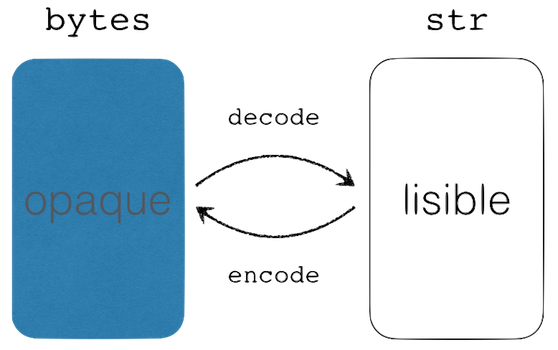
\includegraphics{media/str-bytes.png}
\caption{les types bytes et str}
\end{figure}

    On peut appeler les méthodes \texttt{encode} et \texttt{decode} sans
préciser l'encodage (dans ce cas Python choisit l'encodage par défaut
sur votre système). Cela dit, il est de loin préférable d'être explicite
et de choisir son encodage. En cas de doute, il est recommandé de
\textbf{spécifier explicitement} \texttt{utf-8}, qui se généralise au
détriment d'encodages anciens comme \texttt{cp1242} (Windows) et
\texttt{iso8859-*}, que de laisser le système hôte choisir pour vous.

    \hypertarget{utilisation-des-accents-et-autres-cuxe9dilles}{%
\subparagraph{Utilisation des accents et autres
cédilles}\label{utilisation-des-accents-et-autres-cuxe9dilles}}

    Python 3 supporte Unicode par défaut. Vous pouvez donc, maintenant,
utiliser sans aucun risque des accents ou des cédilles dans vos chaînes
de caractères. Il faut cependant faire attention à deux choses~:

\begin{itemize}
\tightlist
\item
  Python supporte Unicode, donc tous les caractères du monde, mais les
  ordinateurs n'ont pas forcément les polices de caractères nécessaires
  pour afficher ces caractères~;
\item
  Python permet d'utiliser des caractères Unicode pour les noms de
  variables, mais nous vous recommandons dans toute la mesure du
  possible d'écrire votre code en anglais, comme c'est le cas pour la
  quasi-totalité du code que vous serez amenés à utiliser sous forme de
  bibliothèques. Ceci est particulièrement important pour les noms de
  lignes et de colonnes dans un dataset afin de faciliter les transferts
  entre logiciels, la majorité des logiciels n'acceptant pas les accents
  et cédilles dans les noms de variables.
\end{itemize}

Ainsi, il faut bien distinguer les chaînes de caractères qui doivent par
nature être adaptées au langage des utilisateurs du programme, et le
code source qui lui est destiné aux programmeurs et qui doit donc éviter
d'utiliser autre chose que de l'anglais.

    \hypertarget{compluxe9ment---niveau-intermuxe9diaire}{%
\subsection{Complément - niveau
intermédiaire}\label{compluxe9ment---niveau-intermuxe9diaire}}

    \hypertarget{ouxf9-peut-on-mettre-des-accents}{%
\subsubsection{Où peut-on mettre des
accents~?}\label{ouxf9-peut-on-mettre-des-accents}}

    Cela étant dit, si vous devez vraiment mettre des accents dans vos
sources, voici ce qu'il faut savoir.

    \hypertarget{noms-de-variables}{%
\paragraph{Noms de variables}\label{noms-de-variables}}

    \begin{itemize}
\tightlist
\item
  S'il n'était \textbf{pas possible en Python 2} d'utiliser un caractère
  accentué dans un \textbf{nom de variable} (ou d'un identificateur au
  sens large), cela est à présent \textbf{permis en Python 3}~:
\end{itemize}

    \begin{Verbatim}[commandchars=\\\{\},frame=single,framerule=0.3mm,rulecolor=\color{cellframecolor}]
{\color{incolor}In [{\color{incolor}1}]:} \PY{c+c1}{\PYZsh{} pas recommandé, mais autorisé par le langage}
        \PY{n}{nb\PYZus{}élèves} \PY{o}{=} \PY{l+m+mi}{12}
\end{Verbatim}


    \begin{itemize}
\tightlist
\item
  On peut même utiliser des symboles, comme par exemple
\end{itemize}

    \begin{Verbatim}[commandchars=\\\{\},frame=single,framerule=0.3mm,rulecolor=\color{cellframecolor}]
{\color{incolor}In [{\color{incolor}2}]:} \PY{k+kn}{from} \PY{n+nn}{math} \PY{k}{import} \PY{n}{cos}\PY{p}{,} \PY{n}{pi} \PY{k}{as} \PY{n}{𝞟}
        \PY{n}{θ} \PY{o}{=} \PY{n}{𝞟} \PY{o}{/} \PY{l+m+mi}{4}
        \PY{n}{cos}\PY{p}{(}\PY{n}{θ}\PY{p}{)}
\end{Verbatim}


\begin{Verbatim}[commandchars=\\\{\},frame=single,framerule=0.3mm,rulecolor=\color{cellframecolor}]
{\color{outcolor}Out[{\color{outcolor}2}]:} 0.7071067811865476
\end{Verbatim}
            
    \begin{itemize}
\tightlist
\item
  Je vous recommande toutefois de \textbf{ne pas utiliser} cette
  possibilité, si vous n'êtes pas extrêmement familier avec les
  caractères Unicode.
\end{itemize}

    \begin{itemize}
\tightlist
\item
  Enfin, pour être exhaustif, sachez que seule une partie des caractères
  Unicode sont autorisés dans ce cadre, c'est heureux parce que les
  caractères comme, par exemple,
  \href{http://www.fileformat.info/info/unicode/char/a0/index.htm}{l'espace
  non-sécable} pourraient, s'ils étaient autorisés, être la cause de
  milliers d'heures de debugging à frustration garantie :)
\end{itemize}

Pour les curieux, vous pouvez en savoir plus
\href{https://docs.python.org/3/reference/lexical_analysis.html\#identifiers}{à
cet endroit de la documentation officielle (en anglais)}.

    \hypertarget{chauxeenes-de-caractuxe8res}{%
\paragraph{Chaînes de caractères}\label{chauxeenes-de-caractuxe8res}}

    \begin{itemize}
\item
  Vous pouvez naturellement mettre des accents dans les chaînes de
  caractères. Cela dit, les données manipulées par un programme
  proviennent pour l'essentiel de sources externes, comme une base de
  données ou un formulaire Web, et donc le plus souvent pas directement
  du code source. Les chaînes de caractères présentes dans du vrai code
  sont bien souvent limitées à des messages de logging, et le plus
  souvent d'ailleurs en anglais, donc sans accent.
\item
  Lorsque votre programme doit interagir avec les utilisateurs et qu'il
  doit donc parler leur langue, c'est une bonne pratique de créer un
  fichier spécifique, que l'on appelle fichier de ressources, qui
  contient toutes les chaînes de caractères spécifiques à une langue.
  Ainsi, la traduction de votre programme consistera à simplement
  traduire ce fichier de ressources.
\end{itemize}

    \begin{Shaded}
\begin{Highlighting}[frame=lines,framerule=0.6mm,rulecolor=\color{asisframecolor}]
\NormalTok{message }\OperatorTok{=} \StringTok{"on peut mettre un caractère accentué dans une chaîne"}
\end{Highlighting}
\end{Shaded}

    \hypertarget{commentaires}{%
\paragraph{Commentaires}\label{commentaires}}

    \begin{itemize}
\tightlist
\item
  Enfin on peut aussi bien sûr mettre dans les commentaires n'importe
  quel caractère Unicode, et donc notamment des caractères accentués si
  on choisit malgré tout d'écrire le code en français.
\end{itemize}

    \begin{Shaded}
\begin{Highlighting}[frame=lines,framerule=0.6mm,rulecolor=\color{asisframecolor}]
\CommentTok{# on peut mettre un caractère accentué dans un commentaire}
\CommentTok{# ainsi que cos(Θ), ∀x ∈ ∫f(t)dt vous voyez l'idée générale}
\end{Highlighting}
\end{Shaded}

    \hypertarget{quest-ce-quun-encodage}{%
\subsubsection{Qu'est-ce qu'un
encodage~?}\label{quest-ce-quun-encodage}}

    Comme vous le savez, la mémoire - ou le disque - d'un ordinateur ne
permet que de stocker des représentations binaires. Il n'y a donc pas de
façon ``naturelle'' de représenter un caractère comme `A', un guillemet
ou un point-virgule.

On utilise pour cela un encodage, par exemple
\href{http://www.asciitable.com/}{le code \texttt{US-ASCII}} stipule,
pour faire simple, qu'un `A' est représenté par l'octet 65 qui s'écrit
en binaire 01000001. Il se trouve qu'il existe plusieurs encodages, bien
sûr incompatibles, selon les systèmes et les langues. Vous trouverez
plus de détails ci-dessous.

Le point important est que pour pouvoir ouvrir un fichier
``proprement'', il faut bien entendu disposer du \textbf{contenu} du
fichier, mais il faut aussi connaître l'\textbf{encodage} qui a été
utilisé pour l'écrire.

    \hypertarget{pruxe9cautions-uxe0-prendre-pour-lencodage-de-votre-code-source}{%
\subsubsection{Précautions à prendre pour l'encodage de votre code
source}\label{pruxe9cautions-uxe0-prendre-pour-lencodage-de-votre-code-source}}

    L'encodage ne concerne pas simplement les objets chaîne de caractères,
mais également votre code source. \textbf{Python 3} considère que votre
code source utilise \textbf{par défaut l'encodage \texttt{UTF-8}}. Nous
vous conseillons de conserver cet encodage qui est celui qui vous
offrira le plus de flexibilité.

    Vous pouvez malgré tout changer l'encodage \textbf{de votre code source}
en faisant figurer dans vos fichiers, \textbf{en première ou deuxième
ligne}, une déclaration comme ceci~:

\begin{Shaded}
\begin{Highlighting}[frame=lines,framerule=0.6mm,rulecolor=\color{asisframecolor}]
\CommentTok{# -*- coding: <nom_de_l_encodage> -*-}
\end{Highlighting}
\end{Shaded}

ou plus simplement, comme ceci~:

\begin{Shaded}
\begin{Highlighting}[frame=lines,framerule=0.6mm,rulecolor=\color{asisframecolor}]
\CommentTok{# coding: <nom_de_l_encodage>}
\end{Highlighting}
\end{Shaded}

Notons que la première option est également interprétée par l'éditeur de
texte \emph{Emacs} pour utiliser le même encodage. En dehors de
l'utilisation d'Emacs, la deuxième option, plus simple et donc plus
pythonique, est à préférer.

    Le nom \textbf{\texttt{UTF-8}} fait référence à \textbf{Unicode} (ou
pour être précis, à l'encodage le plus répandu parmi ceux qui sont
définis dans la norme Unicode, comme nous le verrons plus bas). Sur
certains systèmes plus anciens vous pourrez être amenés à utiliser un
autre encodage. Pour déterminer la valeur à utiliser dans votre cas
précis vous pouvez faire dans l'interpréteur interactif~:

    \begin{Shaded}
\begin{Highlighting}[frame=lines,framerule=0.6mm,rulecolor=\color{asisframecolor}]
\CommentTok{# ceci doit être exécuté sur votre machine}
\ImportTok{import}\NormalTok{ sys}
\BuiltInTok{print}\NormalTok{(sys.getdefaultencoding())}
\end{Highlighting}
\end{Shaded}

    Par exemple avec d'anciennes versions de Windows (en principe de plus en
plus rares) vous pouvez être amenés à écrire~:

    \begin{Shaded}
\begin{Highlighting}[frame=lines,framerule=0.6mm,rulecolor=\color{asisframecolor}]
\CommentTok{# coding: cp1252}
\end{Highlighting}
\end{Shaded}

    La syntaxe de la ligne \texttt{coding} est précisée dans
\href{https://docs.python.org/3/reference/lexical_analysis.html\#encoding-declarations}{cette
documentation} et dans le
\href{https://www.python.org/dev/peps/pep-0263/}{PEP 263}.

    \hypertarget{le-grand-malentendu}{%
\subsubsection{Le grand malentendu}\label{le-grand-malentendu}}

    Si je vous envoie un fichier contenant du français encodé avec, disons,
\href{http://en.wikipedia.org/wiki/ISO/IEC_8859-15}{ISO/IEC 8859-15 -
a.k.a. \texttt{Latin-9}}; vous pouvez voir dans la table qu'un caractère
`€' va être matérialisé dans mon fichier par un octet `0xA4', soit 164.

Imaginez maintenant que vous essayez d'ouvrir ce même fichier depuis un
vieil ordinateur Windows configuré pour le français. Si on ne lui donne
aucune indication sur l'encodage, le programme qui va lire ce fichier
sur Windows va utiliser l'encodage par défaut du système, c'est-à-dire
\href{http://en.wikipedia.org/wiki/Windows-1252}{CP1252}. Comme vous le
voyez dans cette table, l'octet `0xA4' correspond au caractère

\includegraphics{media/currency-sign.png} et c'est ça que vous allez
voir à la place de €.

Contrairement à ce qu'on pourrait espérer, ce type de problème ne peut
pas se régler en ajoutant une balise
\texttt{\#\ coding:\ \textless{}nom\_de\_l\_encodage\textgreater{}}, qui
n'agit que sur l'encodage utilisé \emph{pour lire le fichier source en
question} (celui qui contient la balise).

Pour régler correctement ce type de problème, il vous faut préciser
explicitement l'encodage à utiliser pour décoder le fichier. Et donc
avoir un moyen fiable de déterminer cet encodage; ce qui n'est pas
toujours aisé d'ailleurs, mais c'est une autre discussion
malheureusement. Ce qui signifie que pour être totalement propre, il
faut pouvoir préciser explicitement le paramètre \texttt{encoding} à
l'appel de toutes les méthodes qui sont susceptibles d'en avoir besoin.

    \hypertarget{pourquoi-uxe7a-marche-en-local}{%
\subsubsection{Pourquoi ça marche en
local~?}\label{pourquoi-uxe7a-marche-en-local}}

    Lorsque le producteur (le programme qui écrit le fichier) et le
consommateur (le programme qui le lit) tournent dans le même ordinateur,
tout fonctionne bien - en général - parce que les deux programmes se
ramènent à l'encodage défini comme l'encodage par défaut.

Il y a toutefois une limite, si vous utilisez un Linux configuré de
manière minimale, il se peut qu'il utilise par défaut l'encodage
\texttt{US-ASCII} - voir plus bas - qui étant très ancien ne ``connaît''
pas un simple é, ni a fortiori €. Pour écrire du français, il faut donc
au minimum que l'encodage par défaut de votre ordinateur contienne les
caractères français, comme par exemple~:

\begin{itemize}
\tightlist
\item
  \texttt{ISO\ 8859-1} (\texttt{Latin-1})
\item
  \texttt{ISO\ 8859-15} (\texttt{Latin-9})
\item
  \texttt{UTF-8}
\item
  \texttt{CP1252}
\end{itemize}

À nouveau dans cette liste, il faut clairement préférer UTF-8 lorsque
c'est possible.

    \hypertarget{un-peu-dhistoire-sur-les-encodages}{%
\subsubsection{Un peu d'histoire sur les
encodages}\label{un-peu-dhistoire-sur-les-encodages}}

    \hypertarget{le-code-us-ascii}{%
\subparagraph{\texorpdfstring{Le code
\texttt{US-ASCII}}{Le code US-ASCII}}\label{le-code-us-ascii}}

    Jusque dans les années 1980, les ordinateurs ne parlaient pour
l'essentiel que l'anglais. La première vague de standardisation avait
créé l'encodage dit \texttt{ASCII}, ou encore \texttt{US-ASCII}
\href{http://www.asciitable.com}{voir par exemple ici}, ou encore
\href{http://en.wikipedia.org/wiki/ASCII}{en version longue ici}.

Le code \texttt{US-ASCII} s'étend sur 128 valeurs, soit 7 bits, mais est
le plus souvent implémenté sur un octet pour préserver l'alignement, le
dernier bit pouvant être utilisé par exemple pour ajouter un code
correcteur d'erreur - ce qui à l'époque des modems n'était pas superflu.
Bref, la pratique courante était alors de manipuler une chaîne de
caractères comme un tableau d'octets.

    \hypertarget{les-encodages-iso8859--latin}{%
\subparagraph{\texorpdfstring{Les encodages \texttt{ISO8859-*}
(\texttt{Latin*})}{Les encodages ISO8859-* (Latin*)}}\label{les-encodages-iso8859--latin}}

    Dans les années 1990, pour satisfaire les besoins des pays européens,
ont été définis plusieurs encodages alternatifs, connus sous le nom de
\href{http://en.wikipedia.org/wiki/ISO/IEC_8859}{\texttt{ISO/IEC\ 8859-*}},
nommés aussi \texttt{Latin-*}. Idéalement, on aurait pu et
\textbf{certainement dû} définir un seul encodage pour représenter tous
les nouveaux caractères, mais entre toutes les langues européennes, le
nombre de caractères à ajouter était substantiel, et cet encodage unifié
aurait largement dépassé 256 caractères différents, il n'aurait donc
\textbf{pas été possible} de tout faire tenir sur un octet.

On a préféré préserver la ``bonne propriété'' du modèle \emph{un
caractère} == \emph{un octet}, ceci afin de préserver le code existant
qui aurait sinon dû être retouché ou réécrit.

Dès lors il n'y avait pas d'autre choix que de définir
\textbf{plusieurs} encodages distincts, par exemple, pour le français on
a utilisé à l'époque
\href{http://en.wikipedia.org/wiki/ISO/IEC_8859-1}{\texttt{ISO/IEC\ 8859-1}
(\texttt{Latin-1})}, pour le russe
\href{http://en.wikipedia.org/wiki/ISO/IEC_8859-5}{\texttt{ISO/IEC\ 5589-5}
(\texttt{Latin/Cyrillic})}.

À ce stade, le ver était dans le fruit. Depuis cette époque pour ouvrir
un fichier il faut connaître son encodage.

    \hypertarget{unicode}{%
\subparagraph{Unicode}\label{unicode}}

    Lorsque l'on a ensuite cherché à manipuler aussi les langues asiatiques,
il a de toute façon fallu définir de nouveaux encodages beaucoup plus
larges. C'est ce qui a été fait par le standard
\href{http://en.wikipedia.org/wiki/Unicode}{Unicode} qui définit 3
nouveaux encodages~:

\begin{itemize}
\tightlist
\item
  \href{http://en.wikipedia.org/wiki/UTF-8}{\texttt{UTF-8}} : un
  encodage à taille variable, à base d'octets, qui maximise la
  compatibilité avec US-ASCII~;
\item
  \href{http://en.wikipedia.org/wiki/UTF-16}{\texttt{UTF-16}} : un
  encodage à taille variable, à base de mots de 16 bits~;
\item
  \href{http://en.wikipedia.org/wiki/UTF-32}{\texttt{UTF-32}} : un
  encodage à taille fixe, à base de mots de 32 bits~;
\end{itemize}

Ces 3 standards couvrent le même jeu de caractères (113 021 tout de même
dans la dernière version). Parmi ceux-ci le plus utilisé est
certainement \texttt{UTF-8}. Un texte ne contenant que des caractères du
code \texttt{US-ASCII} initial peut être lu avec l'encodage
\texttt{UTF-8}.

Pour être enfin tout à fait exhaustif, si on sait qu'un fichier est au
format Unicode, on peut déterminer quel est l'encodage qu'il utilise, en
se basant sur les 4 premiers octets du document. Ainsi dans ce cas
particulier (lorsqu'on est sûr qu'un document utilise un des trois
encodages Unicode) il n'est plus nécessaire de connaître son encodage de
manière ``externe''.


    % Add a bibliography block to the postdoc
    
    
    
   
        \hypertarget{les-outils-de-base-sur-les-chauxeenes-de-caractuxe8res-str}{%
\section{\texorpdfstring{Les outils de base sur les chaînes de
caractères
(\texttt{str})}{Les outils de base sur les chaînes de caractères (str)}}\label{les-outils-de-base-sur-les-chauxeenes-de-caractuxe8res-str}}

    \hypertarget{compluxe9ment---niveau-intermuxe9diaire}{%
\subsection{Complément - niveau
intermédiaire}\label{compluxe9ment---niveau-intermuxe9diaire}}

    \hypertarget{lire-la-documentation}{%
\subsubsection{Lire la documentation}\label{lire-la-documentation}}

    Même après des années de pratique, il est difficile de se souvenir de
toutes les méthodes travaillant sur les chaînes de caractères. Aussi il
est toujours utile de recourir à la documentation embarquée

    \begin{Verbatim}[commandchars=\\\{\}]
{\color{incolor}In [{\color{incolor}1}]:} \PY{n}{help}\PY{p}{(}\PY{n+nb}{str}\PY{p}{)}
\end{Verbatim}


    Nous allons tenter ici de citer les méthodes les plus utilisées. Nous
n'avons le temps que de les utiliser de manière très simple, mais bien
souvent il est possible de passer en argument des options permettant de
ne travailler que sur une sous-chaîne, ou sur la première ou dernière
occurrence d'une sous-chaîne. Nous vous renvoyons à la documentation
pour obtenir toutes les précisions utiles.

    \hypertarget{duxe9coupage---assemblage-split-et-join}{%
\subsubsection{\texorpdfstring{Découpage - assemblage~: \texttt{split}
et
\texttt{join}}{Découpage - assemblage~: split et join}}\label{duxe9coupage---assemblage-split-et-join}}

    Les méthodes \texttt{split} et \texttt{join} permettent de découper une
chaîne selon un séparateur pour obtenir une liste, et à l'inverse de
reconstruire une chaîne à partir d'une liste.

    \texttt{split} permet donc de découper~:

    \begin{Verbatim}[commandchars=\\\{\}]
{\color{incolor}In [{\color{incolor}2}]:} \PY{l+s+s1}{\PYZsq{}}\PY{l+s+s1}{abc=:=def=:=ghi=:=jkl}\PY{l+s+s1}{\PYZsq{}}\PY{o}{.}\PY{n}{split}\PY{p}{(}\PY{l+s+s1}{\PYZsq{}}\PY{l+s+s1}{=:=}\PY{l+s+s1}{\PYZsq{}}\PY{p}{)}
\end{Verbatim}


\begin{Verbatim}[commandchars=\\\{\}]
{\color{outcolor}Out[{\color{outcolor}2}]:} ['abc', 'def', 'ghi', 'jkl']
\end{Verbatim}
            
    Et à l'inverse~:

    \begin{Verbatim}[commandchars=\\\{\}]
{\color{incolor}In [{\color{incolor}3}]:} \PY{l+s+s2}{\PYZdq{}}\PY{l+s+s2}{=:=}\PY{l+s+s2}{\PYZdq{}}\PY{o}{.}\PY{n}{join}\PY{p}{(}\PY{p}{[}\PY{l+s+s1}{\PYZsq{}}\PY{l+s+s1}{abc}\PY{l+s+s1}{\PYZsq{}}\PY{p}{,} \PY{l+s+s1}{\PYZsq{}}\PY{l+s+s1}{def}\PY{l+s+s1}{\PYZsq{}}\PY{p}{,} \PY{l+s+s1}{\PYZsq{}}\PY{l+s+s1}{ghi}\PY{l+s+s1}{\PYZsq{}}\PY{p}{,} \PY{l+s+s1}{\PYZsq{}}\PY{l+s+s1}{jkl}\PY{l+s+s1}{\PYZsq{}}\PY{p}{]}\PY{p}{)}
\end{Verbatim}


\begin{Verbatim}[commandchars=\\\{\}]
{\color{outcolor}Out[{\color{outcolor}3}]:} 'abc=:=def=:=ghi=:=jkl'
\end{Verbatim}
            
    Attention toutefois si le séparateur est un terminateur, la liste
résultat contient alors une dernière chaîne vide. En pratique, on
utilisera la méthode \texttt{strip}, que nous allons voir ci-dessous,
avant la méthode \texttt{split} pour éviter ce problème.

    \begin{Verbatim}[commandchars=\\\{\}]
{\color{incolor}In [{\color{incolor}4}]:} \PY{l+s+s1}{\PYZsq{}}\PY{l+s+s1}{abc;def;ghi;jkl;}\PY{l+s+s1}{\PYZsq{}}\PY{o}{.}\PY{n}{split}\PY{p}{(}\PY{l+s+s1}{\PYZsq{}}\PY{l+s+s1}{;}\PY{l+s+s1}{\PYZsq{}}\PY{p}{)}
\end{Verbatim}


\begin{Verbatim}[commandchars=\\\{\}]
{\color{outcolor}Out[{\color{outcolor}4}]:} ['abc', 'def', 'ghi', 'jkl', '']
\end{Verbatim}
            
    Qui s'inverse correctement cependant~:

    \begin{Verbatim}[commandchars=\\\{\}]
{\color{incolor}In [{\color{incolor}5}]:} \PY{l+s+s2}{\PYZdq{}}\PY{l+s+s2}{;}\PY{l+s+s2}{\PYZdq{}}\PY{o}{.}\PY{n}{join}\PY{p}{(}\PY{p}{[}\PY{l+s+s1}{\PYZsq{}}\PY{l+s+s1}{abc}\PY{l+s+s1}{\PYZsq{}}\PY{p}{,} \PY{l+s+s1}{\PYZsq{}}\PY{l+s+s1}{def}\PY{l+s+s1}{\PYZsq{}}\PY{p}{,} \PY{l+s+s1}{\PYZsq{}}\PY{l+s+s1}{ghi}\PY{l+s+s1}{\PYZsq{}}\PY{p}{,} \PY{l+s+s1}{\PYZsq{}}\PY{l+s+s1}{jkl}\PY{l+s+s1}{\PYZsq{}}\PY{p}{,} \PY{l+s+s1}{\PYZsq{}}\PY{l+s+s1}{\PYZsq{}}\PY{p}{]}\PY{p}{)}
\end{Verbatim}


\begin{Verbatim}[commandchars=\\\{\}]
{\color{outcolor}Out[{\color{outcolor}5}]:} 'abc;def;ghi;jkl;'
\end{Verbatim}
            
    \hypertarget{remplacement-replace}{%
\subsubsection{\texorpdfstring{Remplacement~:
\texttt{replace}}{Remplacement~: replace}}\label{remplacement-replace}}

    \texttt{replace} est très pratique pour remplacer une sous-chaîne par
une autre, avec une limite éventuelle sur le nombre de remplacements~:

    \begin{Verbatim}[commandchars=\\\{\}]
{\color{incolor}In [{\color{incolor}6}]:} \PY{l+s+s2}{\PYZdq{}}\PY{l+s+s2}{abcdefabcdefabcdef}\PY{l+s+s2}{\PYZdq{}}\PY{o}{.}\PY{n}{replace}\PY{p}{(}\PY{l+s+s2}{\PYZdq{}}\PY{l+s+s2}{abc}\PY{l+s+s2}{\PYZdq{}}\PY{p}{,} \PY{l+s+s2}{\PYZdq{}}\PY{l+s+s2}{zoo}\PY{l+s+s2}{\PYZdq{}}\PY{p}{)}
\end{Verbatim}


\begin{Verbatim}[commandchars=\\\{\}]
{\color{outcolor}Out[{\color{outcolor}6}]:} 'zoodefzoodefzoodef'
\end{Verbatim}
            
    \begin{Verbatim}[commandchars=\\\{\}]
{\color{incolor}In [{\color{incolor}7}]:} \PY{l+s+s2}{\PYZdq{}}\PY{l+s+s2}{abcdefabcdefabcdef}\PY{l+s+s2}{\PYZdq{}}\PY{o}{.}\PY{n}{replace}\PY{p}{(}\PY{l+s+s2}{\PYZdq{}}\PY{l+s+s2}{abc}\PY{l+s+s2}{\PYZdq{}}\PY{p}{,} \PY{l+s+s2}{\PYZdq{}}\PY{l+s+s2}{zoo}\PY{l+s+s2}{\PYZdq{}}\PY{p}{,} \PY{l+m+mi}{2}\PY{p}{)}
\end{Verbatim}


\begin{Verbatim}[commandchars=\\\{\}]
{\color{outcolor}Out[{\color{outcolor}7}]:} 'zoodefzoodefabcdef'
\end{Verbatim}
            
    Plusieurs appels à \texttt{replace} peuvent être chaînés comme ceci~:

    \begin{Verbatim}[commandchars=\\\{\}]
{\color{incolor}In [{\color{incolor}8}]:} \PY{l+s+s2}{\PYZdq{}}\PY{l+s+s2}{les [x] qui disent [y]}\PY{l+s+s2}{\PYZdq{}}\PY{o}{.}\PY{n}{replace}\PY{p}{(}\PY{l+s+s2}{\PYZdq{}}\PY{l+s+s2}{[x]}\PY{l+s+s2}{\PYZdq{}}\PY{p}{,} \PY{l+s+s2}{\PYZdq{}}\PY{l+s+s2}{chevaliers}\PY{l+s+s2}{\PYZdq{}}\PY{p}{)}\PY{o}{.}\PY{n}{replace}\PY{p}{(}\PY{l+s+s2}{\PYZdq{}}\PY{l+s+s2}{[y]}\PY{l+s+s2}{\PYZdq{}}\PY{p}{,} \PY{l+s+s2}{\PYZdq{}}\PY{l+s+s2}{Ni}\PY{l+s+s2}{\PYZdq{}}\PY{p}{)}
\end{Verbatim}


\begin{Verbatim}[commandchars=\\\{\}]
{\color{outcolor}Out[{\color{outcolor}8}]:} 'les chevaliers qui disent Ni'
\end{Verbatim}
            
    \hypertarget{nettoyage-strip}{%
\subsubsection{\texorpdfstring{Nettoyage~:
\texttt{strip}}{Nettoyage~: strip}}\label{nettoyage-strip}}

    On pourrait par exemple utiliser \texttt{replace} pour enlever les
espaces dans une chaîne, ce qui peut être utile pour ``nettoyer'' comme
ceci~:

    \begin{Verbatim}[commandchars=\\\{\}]
{\color{incolor}In [{\color{incolor}9}]:} \PY{l+s+s2}{\PYZdq{}}\PY{l+s+s2}{ abc:def:ghi }\PY{l+s+s2}{\PYZdq{}}\PY{o}{.}\PY{n}{replace}\PY{p}{(}\PY{l+s+s2}{\PYZdq{}}\PY{l+s+s2}{ }\PY{l+s+s2}{\PYZdq{}}\PY{p}{,} \PY{l+s+s2}{\PYZdq{}}\PY{l+s+s2}{\PYZdq{}}\PY{p}{)}
\end{Verbatim}


\begin{Verbatim}[commandchars=\\\{\}]
{\color{outcolor}Out[{\color{outcolor}9}]:} 'abc:def:ghi'
\end{Verbatim}
            
    Toutefois bien souvent on préfère utiliser \texttt{strip} qui ne
s'occupe que du début et de la fin de la chaîne, et gère aussi les
tabulations et autres retour à la ligne~:

    \begin{Verbatim}[commandchars=\\\{\}]
{\color{incolor}In [{\color{incolor}10}]:} \PY{l+s+s2}{\PYZdq{}}\PY{l+s+s2}{ }\PY{l+s+se}{\PYZbs{}t}\PY{l+s+s2}{une chaîne avec des trucs qui dépassent }\PY{l+s+se}{\PYZbs{}n}\PY{l+s+s2}{\PYZdq{}}\PY{o}{.}\PY{n}{strip}\PY{p}{(}\PY{p}{)}
\end{Verbatim}


\begin{Verbatim}[commandchars=\\\{\}]
{\color{outcolor}Out[{\color{outcolor}10}]:} 'une chaîne avec des trucs qui dépassent'
\end{Verbatim}
            
    On peut appliquer \texttt{strip} avant \texttt{split} pour éviter le
problème du dernier élément vide~:

    \begin{Verbatim}[commandchars=\\\{\}]
{\color{incolor}In [{\color{incolor}11}]:} \PY{l+s+s1}{\PYZsq{}}\PY{l+s+s1}{abc;def;ghi;jkl;}\PY{l+s+s1}{\PYZsq{}}\PY{o}{.}\PY{n}{strip}\PY{p}{(}\PY{l+s+s1}{\PYZsq{}}\PY{l+s+s1}{;}\PY{l+s+s1}{\PYZsq{}}\PY{p}{)}\PY{o}{.}\PY{n}{split}\PY{p}{(}\PY{l+s+s1}{\PYZsq{}}\PY{l+s+s1}{;}\PY{l+s+s1}{\PYZsq{}}\PY{p}{)}
\end{Verbatim}


\begin{Verbatim}[commandchars=\\\{\}]
{\color{outcolor}Out[{\color{outcolor}11}]:} ['abc', 'def', 'ghi', 'jkl']
\end{Verbatim}
            
    \hypertarget{rechercher-une-sous-chauxeene}{%
\subsubsection{Rechercher une
sous-chaîne}\label{rechercher-une-sous-chauxeene}}

    Plusieurs outils permettent de chercher une sous-chaîne. Il existe
\texttt{find} qui renvoie le plus petit index où on trouve la
sous-chaîne~:

    \begin{Verbatim}[commandchars=\\\{\}]
{\color{incolor}In [{\color{incolor}12}]:} \PY{c+c1}{\PYZsh{} l\PYZsq{}indice du début de la première occurrence}
         \PY{l+s+s2}{\PYZdq{}}\PY{l+s+s2}{abcdefcdefghefghijk}\PY{l+s+s2}{\PYZdq{}}\PY{o}{.}\PY{n}{find}\PY{p}{(}\PY{l+s+s2}{\PYZdq{}}\PY{l+s+s2}{def}\PY{l+s+s2}{\PYZdq{}}\PY{p}{)}
\end{Verbatim}


\begin{Verbatim}[commandchars=\\\{\}]
{\color{outcolor}Out[{\color{outcolor}12}]:} 3
\end{Verbatim}
            
    \begin{Verbatim}[commandchars=\\\{\}]
{\color{incolor}In [{\color{incolor}13}]:} \PY{c+c1}{\PYZsh{} ou \PYZhy{}1 si la chaîne n\PYZsq{}est pas présente}
         \PY{l+s+s2}{\PYZdq{}}\PY{l+s+s2}{abcdefcdefghefghijk}\PY{l+s+s2}{\PYZdq{}}\PY{o}{.}\PY{n}{find}\PY{p}{(}\PY{l+s+s2}{\PYZdq{}}\PY{l+s+s2}{zoo}\PY{l+s+s2}{\PYZdq{}}\PY{p}{)}
\end{Verbatim}


\begin{Verbatim}[commandchars=\\\{\}]
{\color{outcolor}Out[{\color{outcolor}13}]:} -1
\end{Verbatim}
            
    \texttt{rfind} fonctionne comme \texttt{find} mais en partant de la fin
de la chaîne~:

    \begin{Verbatim}[commandchars=\\\{\}]
{\color{incolor}In [{\color{incolor}14}]:} \PY{c+c1}{\PYZsh{} en partant de la fin}
         \PY{l+s+s2}{\PYZdq{}}\PY{l+s+s2}{abcdefcdefghefghijk}\PY{l+s+s2}{\PYZdq{}}\PY{o}{.}\PY{n}{rfind}\PY{p}{(}\PY{l+s+s2}{\PYZdq{}}\PY{l+s+s2}{fgh}\PY{l+s+s2}{\PYZdq{}}\PY{p}{)}
\end{Verbatim}


\begin{Verbatim}[commandchars=\\\{\}]
{\color{outcolor}Out[{\color{outcolor}14}]:} 13
\end{Verbatim}
            
    \begin{Verbatim}[commandchars=\\\{\}]
{\color{incolor}In [{\color{incolor}15}]:} \PY{c+c1}{\PYZsh{} notez que le résultat correspond}
         \PY{c+c1}{\PYZsh{} tout de même toujours au début de la chaîne}
         \PY{c+c1}{\PYZsh{} NB: en python les indices commencent à zéro}
         \PY{c+c1}{\PYZsh{} donc la notation ma\PYZus{}chaine[n] permet d\PYZsq{}accèder au n+1 ème caractère de la chaine}
         \PY{l+s+s2}{\PYZdq{}}\PY{l+s+s2}{abcdefcdefghefghijk}\PY{l+s+s2}{\PYZdq{}}\PY{p}{[}\PY{l+m+mi}{13}\PY{p}{]}
\end{Verbatim}


\begin{Verbatim}[commandchars=\\\{\}]
{\color{outcolor}Out[{\color{outcolor}15}]:} 'f'
\end{Verbatim}
            
    La méthode \texttt{index} se comporte comme \texttt{find}, mais en cas
d'absence elle lève une \textbf{exception} (nous verrons ce concept plus
tard) plutôt que de renvoyer \texttt{-1}~:

    \begin{Verbatim}[commandchars=\\\{\}]
{\color{incolor}In [{\color{incolor}16}]:} \PY{l+s+s2}{\PYZdq{}}\PY{l+s+s2}{abcdefcdefghefghijk}\PY{l+s+s2}{\PYZdq{}}\PY{o}{.}\PY{n}{index}\PY{p}{(}\PY{l+s+s2}{\PYZdq{}}\PY{l+s+s2}{def}\PY{l+s+s2}{\PYZdq{}}\PY{p}{)}
\end{Verbatim}


\begin{Verbatim}[commandchars=\\\{\}]
{\color{outcolor}Out[{\color{outcolor}16}]:} 3
\end{Verbatim}
            
    \begin{Verbatim}[commandchars=\\\{\}]
{\color{incolor}In [{\color{incolor}17}]:} \PY{k}{try}\PY{p}{:}
             \PY{l+s+s2}{\PYZdq{}}\PY{l+s+s2}{abcdefcdefghefghijk}\PY{l+s+s2}{\PYZdq{}}\PY{o}{.}\PY{n}{index}\PY{p}{(}\PY{l+s+s2}{\PYZdq{}}\PY{l+s+s2}{zoo}\PY{l+s+s2}{\PYZdq{}}\PY{p}{)}
         \PY{k}{except} \PY{n+ne}{Exception} \PY{k}{as} \PY{n}{e}\PY{p}{:}
             \PY{n+nb}{print}\PY{p}{(}\PY{l+s+s2}{\PYZdq{}}\PY{l+s+s2}{OOPS}\PY{l+s+s2}{\PYZdq{}}\PY{p}{,} \PY{n+nb}{type}\PY{p}{(}\PY{n}{e}\PY{p}{)}\PY{p}{,} \PY{n}{e}\PY{p}{)}
\end{Verbatim}


    \begin{Verbatim}[commandchars=\\\{\}]
OOPS <class 'ValueError'> substring not found

    \end{Verbatim}

    Mais le plus simple pour chercher si une sous-chaîne est dans une autre
chaîne est d'utiliser l'instruction \texttt{in} sur laquelle nous
reviendrons lorsque nous parlerons des séquences~:

    \begin{Verbatim}[commandchars=\\\{\}]
{\color{incolor}In [{\color{incolor}18}]:} \PY{l+s+s2}{\PYZdq{}}\PY{l+s+s2}{def}\PY{l+s+s2}{\PYZdq{}} \PY{o+ow}{in} \PY{l+s+s2}{\PYZdq{}}\PY{l+s+s2}{abcdefcdefghefghijk}\PY{l+s+s2}{\PYZdq{}}
\end{Verbatim}


\begin{Verbatim}[commandchars=\\\{\}]
{\color{outcolor}Out[{\color{outcolor}18}]:} True
\end{Verbatim}
            
    La méthode \texttt{count} compte le nombre d'occurrences d'une
sous-chaîne~:

    \begin{Verbatim}[commandchars=\\\{\}]
{\color{incolor}In [{\color{incolor}19}]:} \PY{l+s+s2}{\PYZdq{}}\PY{l+s+s2}{abcdefcdefghefghijk}\PY{l+s+s2}{\PYZdq{}}\PY{o}{.}\PY{n}{count}\PY{p}{(}\PY{l+s+s2}{\PYZdq{}}\PY{l+s+s2}{ef}\PY{l+s+s2}{\PYZdq{}}\PY{p}{)}
\end{Verbatim}


\begin{Verbatim}[commandchars=\\\{\}]
{\color{outcolor}Out[{\color{outcolor}19}]:} 3
\end{Verbatim}
            
    Signalons enfin les méthodes de commodité suivantes~:

    \begin{Verbatim}[commandchars=\\\{\}]
{\color{incolor}In [{\color{incolor}20}]:} \PY{l+s+s2}{\PYZdq{}}\PY{l+s+s2}{abcdefcdefghefghijk}\PY{l+s+s2}{\PYZdq{}}\PY{o}{.}\PY{n}{startswith}\PY{p}{(}\PY{l+s+s2}{\PYZdq{}}\PY{l+s+s2}{abcd}\PY{l+s+s2}{\PYZdq{}}\PY{p}{)}
\end{Verbatim}


\begin{Verbatim}[commandchars=\\\{\}]
{\color{outcolor}Out[{\color{outcolor}20}]:} True
\end{Verbatim}
            
    \begin{Verbatim}[commandchars=\\\{\}]
{\color{incolor}In [{\color{incolor}21}]:} \PY{l+s+s2}{\PYZdq{}}\PY{l+s+s2}{abcdefcdefghefghijk}\PY{l+s+s2}{\PYZdq{}}\PY{o}{.}\PY{n}{endswith}\PY{p}{(}\PY{l+s+s2}{\PYZdq{}}\PY{l+s+s2}{ghijk}\PY{l+s+s2}{\PYZdq{}}\PY{p}{)}
\end{Verbatim}


\begin{Verbatim}[commandchars=\\\{\}]
{\color{outcolor}Out[{\color{outcolor}21}]:} True
\end{Verbatim}
            
    S'agissant des deux dernières, remarquons que~:\\

    \texttt{chaine.startswith(sous\_chaine)} \(\Longleftrightarrow\)
\texttt{chaine.find(sous\_chaine)\ ==\ 0}\\

\texttt{chaine.endswith(sous\_chaine)} \(\Longleftrightarrow\)
\texttt{chaine.rfind(sous\_chaine)\ ==\ (len(chaine)\ -\ len(sous\_chaine))}\\

    On remarque ici la supériorité en terme d'expressivité des méthodes
pythoniques \texttt{startswith} et \texttt{endswith}.

    \hypertarget{changement-de-casse}{%
\subsubsection{Changement de casse}\label{changement-de-casse}}

    Voici pour conclure quelques méthodes utiles qui parlent d'elles-mêmes~:

    \begin{Verbatim}[commandchars=\\\{\}]
{\color{incolor}In [{\color{incolor}22}]:} \PY{l+s+s2}{\PYZdq{}}\PY{l+s+s2}{monty PYTHON}\PY{l+s+s2}{\PYZdq{}}\PY{o}{.}\PY{n}{upper}\PY{p}{(}\PY{p}{)}
\end{Verbatim}


\begin{Verbatim}[commandchars=\\\{\}]
{\color{outcolor}Out[{\color{outcolor}22}]:} 'MONTY PYTHON'
\end{Verbatim}
            
    \begin{Verbatim}[commandchars=\\\{\}]
{\color{incolor}In [{\color{incolor}23}]:} \PY{l+s+s2}{\PYZdq{}}\PY{l+s+s2}{monty PYTHON}\PY{l+s+s2}{\PYZdq{}}\PY{o}{.}\PY{n}{lower}\PY{p}{(}\PY{p}{)}
\end{Verbatim}


\begin{Verbatim}[commandchars=\\\{\}]
{\color{outcolor}Out[{\color{outcolor}23}]:} 'monty python'
\end{Verbatim}
            
    \begin{Verbatim}[commandchars=\\\{\}]
{\color{incolor}In [{\color{incolor}24}]:} \PY{l+s+s2}{\PYZdq{}}\PY{l+s+s2}{monty PYTHON}\PY{l+s+s2}{\PYZdq{}}\PY{o}{.}\PY{n}{swapcase}\PY{p}{(}\PY{p}{)}
\end{Verbatim}


\begin{Verbatim}[commandchars=\\\{\}]
{\color{outcolor}Out[{\color{outcolor}24}]:} 'MONTY python'
\end{Verbatim}
            
    \begin{Verbatim}[commandchars=\\\{\}]
{\color{incolor}In [{\color{incolor}25}]:} \PY{l+s+s2}{\PYZdq{}}\PY{l+s+s2}{monty PYTHON}\PY{l+s+s2}{\PYZdq{}}\PY{o}{.}\PY{n}{capitalize}\PY{p}{(}\PY{p}{)}
\end{Verbatim}


\begin{Verbatim}[commandchars=\\\{\}]
{\color{outcolor}Out[{\color{outcolor}25}]:} 'Monty python'
\end{Verbatim}
            
    \begin{Verbatim}[commandchars=\\\{\}]
{\color{incolor}In [{\color{incolor}26}]:} \PY{l+s+s2}{\PYZdq{}}\PY{l+s+s2}{monty PYTHON}\PY{l+s+s2}{\PYZdq{}}\PY{o}{.}\PY{n}{title}\PY{p}{(}\PY{p}{)}
\end{Verbatim}


\begin{Verbatim}[commandchars=\\\{\}]
{\color{outcolor}Out[{\color{outcolor}26}]:} 'Monty Python'
\end{Verbatim}
            
    \hypertarget{pour-en-savoir-plus}{%
\subsubsection{Pour en savoir plus}\label{pour-en-savoir-plus}}

    Tous ces outils sont
\href{https://docs.python.org/3/library/stdtypes.html\#string-methods}{documentés
en détail ici (en anglais)}.
        \hypertarget{formatage-de-chauxeenes-de-caractuxe8res}{%
\section{Formatage de chaînes de
caractères}\label{formatage-de-chauxeenes-de-caractuxe8res}}

    \hypertarget{compluxe9ment---niveau-basique}{%
\subsection{Complément - niveau
basique}\label{compluxe9ment---niveau-basique}}

    On désigne par formatage les outils qui permettent d'obtenir une
présentation fine des résultats, que ce soit pour améliorer la
lisibilité lorsqu'on s'adresse à des humains, ou pour respecter la
syntaxe d'un outil auquel on veut passer les données pour un traitement
ultérieur.

    \hypertarget{la-fonction-print}{%
\subsubsection{\texorpdfstring{La fonction
\texttt{print}}{La fonction print}}\label{la-fonction-print}}

    Nous avons jusqu'à maintenant presque toujours utilisé la fonction
\texttt{print} pour afficher nos résultats. Comme on l'a vu, celle-ci
réalise un formatage sommaire~: elle insère un espace entre les valeurs
qui lui sont passées.

    \begin{Verbatim}[commandchars=\\\{\}]
{\color{incolor}In [{\color{incolor}1}]:} \PY{n+nb}{print}\PY{p}{(}\PY{l+m+mi}{1}\PY{p}{,} \PY{l+s+s1}{\PYZsq{}}\PY{l+s+s1}{a}\PY{l+s+s1}{\PYZsq{}}\PY{p}{,} \PY{l+m+mi}{12} \PY{o}{+} \PY{l+m+mi}{4}\PY{n}{j}\PY{p}{)}
\end{Verbatim}


    \begin{Verbatim}[commandchars=\\\{\}]
1 a (12+4j)

    \end{Verbatim}

    La seule subtilité notable concernant \texttt{print} est que, par
défaut, elle ajoute un saut de ligne à la fin. Pour éviter ce
comportement, on peut passer à la fonction un argument \texttt{end}, qui
sera inséré \emph{au lieu} du saut de ligne. Ainsi par exemple~:

    \begin{Verbatim}[commandchars=\\\{\}]
{\color{incolor}In [{\color{incolor}2}]:} \PY{c+c1}{\PYZsh{} une première ligne}
        \PY{n+nb}{print}\PY{p}{(}\PY{l+s+s2}{\PYZdq{}}\PY{l+s+s2}{une}\PY{l+s+s2}{\PYZdq{}}\PY{p}{,} \PY{l+s+s2}{\PYZdq{}}\PY{l+s+s2}{seule}\PY{l+s+s2}{\PYZdq{}}\PY{p}{,} \PY{l+s+s2}{\PYZdq{}}\PY{l+s+s2}{ligne}\PY{l+s+s2}{\PYZdq{}}\PY{p}{)}
\end{Verbatim}


    \begin{Verbatim}[commandchars=\\\{\}]
une seule ligne

    \end{Verbatim}

    \begin{Verbatim}[commandchars=\\\{\}]
{\color{incolor}In [{\color{incolor}3}]:} \PY{c+c1}{\PYZsh{} une deuxième ligne en deux appels à print}
        \PY{n+nb}{print}\PY{p}{(}\PY{l+s+s2}{\PYZdq{}}\PY{l+s+s2}{une}\PY{l+s+s2}{\PYZdq{}}\PY{p}{,} \PY{l+s+s2}{\PYZdq{}}\PY{l+s+s2}{autre}\PY{l+s+s2}{\PYZdq{}}\PY{p}{,} \PY{n}{end}\PY{o}{=}\PY{l+s+s1}{\PYZsq{}}\PY{l+s+s1}{ }\PY{l+s+s1}{\PYZsq{}}\PY{p}{)}
        \PY{n+nb}{print}\PY{p}{(}\PY{l+s+s2}{\PYZdq{}}\PY{l+s+s2}{ligne}\PY{l+s+s2}{\PYZdq{}}\PY{p}{)}
\end{Verbatim}


    \begin{Verbatim}[commandchars=\\\{\}]
une autre ligne

    \end{Verbatim}

    Il faut remarquer aussi que \texttt{print} est capable d'imprimer
\textbf{n'importe quel objet}. Nous l'avons déjà fait avec les listes et
les tuples, voici par exemple un module~:

    \begin{Verbatim}[commandchars=\\\{\}]
{\color{incolor}In [{\color{incolor}4}]:} \PY{c+c1}{\PYZsh{} on peut imprimer par exemple un objet \PYZsq{}module\PYZsq{}}
        \PY{k+kn}{import} \PY{n+nn}{math}
        
        \PY{n+nb}{print}\PY{p}{(}\PY{l+s+s1}{\PYZsq{}}\PY{l+s+s1}{le module math est}\PY{l+s+s1}{\PYZsq{}}\PY{p}{,} \PY{n}{math}\PY{p}{)}
\end{Verbatim}


    \begin{Verbatim}[commandchars=\\\{\}]
le module math est <module 'math' (built-in)>

    \end{Verbatim}

    En anticipant un peu, voici comment \texttt{print} présente les
instances de classe (ne vous inquiétez pas, nous apprendrons dans une
semaine ultérieure ce que sont les classes et les instances).

    \begin{Verbatim}[commandchars=\\\{\}]
{\color{incolor}In [{\color{incolor}5}]:} \PY{c+c1}{\PYZsh{} pour définir la classe Personne}
        \PY{k}{class} \PY{n+nc}{Personne}\PY{p}{:}
            \PY{k}{pass}
        
        \PY{c+c1}{\PYZsh{} et pour créer une instance de cette classe}
        \PY{n}{personne} \PY{o}{=} \PY{n}{Personne}\PY{p}{(}\PY{p}{)}
\end{Verbatim}


    \begin{Verbatim}[commandchars=\\\{\}]
{\color{incolor}In [{\color{incolor}6}]:} \PY{c+c1}{\PYZsh{} voilà comment s\PYZsq{}affiche une instance de classe}
        \PY{n+nb}{print}\PY{p}{(}\PY{n}{personne}\PY{p}{)}
\end{Verbatim}


    \begin{Verbatim}[commandchars=\\\{\}]
<\_\_main\_\_.Personne object at 0x04B94EF0>

    \end{Verbatim}

    On rencontre assez vite les limites de \texttt{print}~:

\begin{itemize}
\tightlist
\item
  d'une part, il peut être nécessaire de formater une chaîne de
  caractères sans nécessairement vouloir l'imprimer, ou en tout cas pas
  immédiatement~;
\item
  d'autre part, les espaces ajoutées peuvent être plus néfastes
  qu'utiles~;
\item
  enfin, on peut avoir besoin de préciser un nombre de chiffres
  significatifs, ou de choisir comment présenter une date.
\end{itemize}

C'est pourquoi il est plus courant de \textbf{formater} les chaînes -
c'est-à-dire de calculer des chaînes en mémoire, sans nécessairement les
imprimer de suite, et c'est ce que nous allons étudier dans ce
complément.

    \hypertarget{les-f-strings}, qui sont encore massivement utilisées
dans le code existant (surtout \texttt{\%} d'ailleurs, bien que
essentiellement obsolète).\\

    Mais définissons d'abord quelques données à afficher~:

    \begin{Verbatim}[commandchars=\\\{\}]
{\color{incolor}In [{\color{incolor}7}]:} \PY{c+c1}{\PYZsh{} donnons\PYZhy{}nous quelques variables}
        \PY{n}{prenom}\PY{p}{,} \PY{n}{nom}\PY{p}{,} \PY{n}{age} \PY{o}{=} \PY{l+s+s1}{\PYZsq{}}\PY{l+s+s1}{Jean}\PY{l+s+s1}{\PYZsq{}}\PY{p}{,} \PY{l+s+s1}{\PYZsq{}}\PY{l+s+s1}{Dupont}\PY{l+s+s1}{\PYZsq{}}\PY{p}{,} \PY{l+m+mi}{35}
\end{Verbatim}


    \begin{Verbatim}[commandchars=\\\{\}]
{\color{incolor}In [{\color{incolor}8}]:} \PY{c+c1}{\PYZsh{} mon premier f\PYZhy{}string}
        \PY{n}{f}\PY{l+s+s2}{\PYZdq{}}\PY{l+s+si}{\PYZob{}prenom\PYZcb{}}\PY{l+s+s2}{ }\PY{l+s+si}{\PYZob{}nom\PYZcb{}}\PY{l+s+s2}{ a }\PY{l+s+si}{\PYZob{}age\PYZcb{}}\PY{l+s+s2}{ ans}\PY{l+s+s2}{\PYZdq{}}
\end{Verbatim}


\begin{Verbatim}[commandchars=\\\{\}]
{\color{outcolor}Out[{\color{outcolor}8}]:} 'Jean Dupont a 35 ans'
\end{Verbatim}
            
    Vous remarquez d'abord que la chaine commence par \texttt{f"}, c'est
bien sûr pour cela qu'on l'appelle un \emph{f-string}.\\

On peut bien entendu ajouter le \texttt{f} devant toutes les formes de
strings, qu'ils commencent par \texttt{\textquotesingle{}} ou \texttt{"}
ou \texttt{\textquotesingle{}\textquotesingle{}\textquotesingle{}} ou
\texttt{"""}.\\

    Ensuite vous remarquez que les zones délimitées entre \texttt{\{\}} sont
remplacées. La logique d'un \emph{f-string}, c'est tout simplement de
considérer l'intérieur d'un \texttt{\{\}} comme du code Python (une
expression pour être précis), de l'évaluer, et d'utiliser le résultat
pour remplir le \texttt{\{\}}.\\

    Ça veut dire, en clair, que je peux faire des calculs à l'intérieur des
\texttt{\{\}}.

    \begin{Verbatim}[commandchars=\\\{\}]
{\color{incolor}In [{\color{incolor}9}]:} \PY{c+c1}{\PYZsh{} toutes les expressions sont autorisées à l\PYZsq{}intérieur d\PYZsq{}un \PYZob{}\PYZcb{}}
        \PY{n}{f}\PY{l+s+s2}{\PYZdq{}}\PY{l+s+s2}{dans 10 ans }\PY{l+s+si}{\PYZob{}prenom\PYZcb{}}\PY{l+s+s2}{ aura }\PY{l+s+s2}{\PYZob{}}\PY{l+s+s2}{age + 10\PYZcb{} ans}\PY{l+s+s2}{\PYZdq{}}
\end{Verbatim}


\begin{Verbatim}[commandchars=\\\{\}]
{\color{outcolor}Out[{\color{outcolor}9}]:} 'dans 10 ans Jean aura 45 ans'
\end{Verbatim}
            
    \begin{Verbatim}[commandchars=\\\{\}]
{\color{incolor}In [{\color{incolor}10}]:} \PY{c+c1}{\PYZsh{} on peut donc aussi mettre des appels de fonction}
         \PY{n}{notes} \PY{o}{=} \PY{p}{[}\PY{l+m+mi}{12}\PY{p}{,} \PY{l+m+mi}{15}\PY{p}{,} \PY{l+m+mi}{19}\PY{p}{]}
         \PY{n}{f}\PY{l+s+s2}{\PYZdq{}}\PY{l+s+s2}{nous avons pour l}\PY{l+s+s2}{\PYZsq{}}\PY{l+s+s2}{instant }\PY{l+s+s2}{\PYZob{}}\PY{l+s+s2}{len(notes)\PYZcb{} notes}\PY{l+s+s2}{\PYZdq{}}
\end{Verbatim}


\begin{Verbatim}[commandchars=\\\{\}]
{\color{outcolor}Out[{\color{outcolor}10}]:} "nous avons pour l'instant 3 notes"
\end{Verbatim}
            
    Nous allons en rester là pour la partie en niveau basique. Il nous reste
à étudier comment chaque \texttt{\{\}} est formaté (par exemple comment
choisir le nombre de chiffres significatifs sur un flottant), ce point
est expliqué plus bas.\\

Comme vous le voyez, les \emph{f-strings} fournissent une méthode très
simple et expressive pour formater des données dans des chaînes de
caractère. Redisons-le pour être bien clair~: un \emph{f-string}
\textbf{ne réalise pas d'impression}, il faut donc le passer à
\texttt{print} si l'impression est souhaitée.

    \hypertarget{la-muxe9thode-format}{%
\subsubsection{\texorpdfstring{La méthode
\texttt{format}}{La méthode format}}\label{la-muxe9thode-format}}

    Avant l'introduction des \emph{f-strings}, la technique recommandée pour
faire du formatage était d'utiliser la méthode \texttt{format} qui est
définie sur les objets \texttt{str} et qui s'utilise comme ceci~:

    \begin{Verbatim}[commandchars=\\\{\}]
{\color{incolor}In [{\color{incolor}11}]:} \PY{l+s+s2}{\PYZdq{}}\PY{l+s+si}{\PYZob{}\PYZcb{}}\PY{l+s+s2}{ }\PY{l+s+si}{\PYZob{}\PYZcb{}}\PY{l+s+s2}{ a }\PY{l+s+si}{\PYZob{}\PYZcb{}}\PY{l+s+s2}{ ans}\PY{l+s+s2}{\PYZdq{}}\PY{o}{.}\PY{n}{format}\PY{p}{(}\PY{n}{prenom}\PY{p}{,} \PY{n}{nom}\PY{p}{,} \PY{n}{age}\PY{p}{)}
\end{Verbatim}


\begin{Verbatim}[commandchars=\\\{\}]
{\color{outcolor}Out[{\color{outcolor}11}]:} 'Jean Dupont a 35 ans'
\end{Verbatim}
            
    Dans cet exemple le plus simple, les données sont affichées en lieu et
place des \texttt{\{\}}, dans l'ordre où elles sont fournies.\\

    Cela convient bien lorsqu'on a peu de données. Si par la suite on veut
changer l'ordre par exemple des nom et prénom, on peut bien sûr échanger
l'ordre des arguments passés à format, ou encore utiliser la
\textbf{liaison par position}, comme ceci~:

    \begin{Verbatim}[commandchars=\\\{\}]
{\color{incolor}In [{\color{incolor}12}]:} \PY{l+s+s2}{\PYZdq{}}\PY{l+s+si}{\PYZob{}1\PYZcb{}}\PY{l+s+s2}{ }\PY{l+s+si}{\PYZob{}0\PYZcb{}}\PY{l+s+s2}{ a }\PY{l+s+si}{\PYZob{}2\PYZcb{}}\PY{l+s+s2}{ ans}\PY{l+s+s2}{\PYZdq{}}\PY{o}{.}\PY{n}{format}\PY{p}{(}\PY{n}{prenom}\PY{p}{,} \PY{n}{nom}\PY{p}{,} \PY{n}{age}\PY{p}{)}
\end{Verbatim}


\begin{Verbatim}[commandchars=\\\{\}]
{\color{outcolor}Out[{\color{outcolor}12}]:} 'Dupont Jean a 35 ans'
\end{Verbatim}
            
    Dans la pratique toutefois, cette forme est assez peu utile, on lui
préfère souvent la \textbf{liaison par nom} qui se présente comme ceci~:

    \begin{Verbatim}[commandchars=\\\{\}]
{\color{incolor}In [{\color{incolor}13}]:} \PY{l+s+s2}{\PYZdq{}}\PY{l+s+si}{\PYZob{}le\PYZus{}prenom\PYZcb{}}\PY{l+s+s2}{ }\PY{l+s+si}{\PYZob{}le\PYZus{}nom\PYZcb{}}\PY{l+s+s2}{ a }\PY{l+s+si}{\PYZob{}l\PYZus{}age\PYZcb{}}\PY{l+s+s2}{ ans}\PY{l+s+s2}{\PYZdq{}}\PY{o}{.}\PY{n}{format}\PY{p}{(}\PY{n}{le\PYZus{}nom}\PY{o}{=}\PY{n}{nom}\PY{p}{,} \PY{n}{le\PYZus{}prenom}\PY{o}{=}\PY{n}{prenom}\PY{p}{,} \PY{n}{l\PYZus{}age}\PY{o}{=}\PY{n}{age}\PY{p}{)}
\end{Verbatim}


\begin{Verbatim}[commandchars=\\\{\}]
{\color{outcolor}Out[{\color{outcolor}13}]:} 'Jean Dupont a 35 ans'
\end{Verbatim}
            
    Dans ce premier exemple de liaison par nom, nous avons délibérément
utilisé des noms différents pour les données externes et pour les noms
apparaissant dans le format, pour bien illustrer comment la liaison est
résolue, mais on peut aussi bien faire tout simplement~:

    \begin{Verbatim}[commandchars=\\\{\}]
{\color{incolor}In [{\color{incolor}14}]:} \PY{l+s+s2}{\PYZdq{}}\PY{l+s+si}{\PYZob{}prenom\PYZcb{}}\PY{l+s+s2}{ }\PY{l+s+si}{\PYZob{}nom\PYZcb{}}\PY{l+s+s2}{ a }\PY{l+s+si}{\PYZob{}age\PYZcb{}}\PY{l+s+s2}{ ans}\PY{l+s+s2}{\PYZdq{}}\PY{o}{.}\PY{n}{format}\PY{p}{(}\PY{n}{nom}\PY{o}{=}\PY{n}{nom}\PY{p}{,} \PY{n}{prenom}\PY{o}{=}\PY{n}{prenom}\PY{p}{,} \PY{n}{age}\PY{o}{=}\PY{n}{age}\PY{p}{)}
\end{Verbatim}


\begin{Verbatim}[commandchars=\\\{\}]
{\color{outcolor}Out[{\color{outcolor}14}]:} 'Jean Dupont a 35 ans'
\end{Verbatim}
            
    Voici qui conclut notre courte introduction à la méthode
\texttt{format}.

    \hypertarget{compluxe9ment---niveau-intermuxe9diaire}{%
\subsection{Complément - niveau
intermédiaire}\label{compluxe9ment---niveau-intermuxe9diaire}}

    \hypertarget{la-toute-premiuxe8re-version-du-formatage-lopuxe9rateur}}{La toute première version du formatage~: l'opérateur \%}}\label{la-toute-premiuxe8re-version-du-formatage-lopuxe9rateur}}

    \texttt{format} a été en fait introduite assez tard dans Python, pour
remplacer la technique que nous allons présenter maintenant.\\

Étant donné le volume de code qui a été écrit avec l'opérateur
\texttt{\%}, il nous a semblé important d'introduire brièvement cette
construction ici. Vous ne devez cependant pas utiliser cet opérateur
dans du code moderne, la manière pythonique de formater les chaînes de
caractères est le f-string.\\

    Le principe de l'opérateur \texttt{\%} est le suivant. On élabore comme
ci-dessus un ``format'' c'est-à-dire le patron de ce qui doit être
rendu, auquel on passe des arguments pour ``remplir'' les trous. Voyons
les exemples de tout à l'heure avec l'opérateur \texttt{\%}~:

    \begin{Verbatim}[commandchars=\\\{\}]
{\color{incolor}In [{\color{incolor}15}]:} \PY{c+c1}{\PYZsh{} l\PYZsq{}ancienne façon de formater les chaînes avec \PYZpc{}}
         \PY{c+c1}{\PYZsh{} est souvent moins lisible}
         \PY{l+s+s2}{\PYZdq{}}\PY{l+s+si}{\PYZpc{}s}\PY{l+s+s2}{ }\PY{l+s+si}{\PYZpc{}s}\PY{l+s+s2}{ a }\PY{l+s+si}{\PYZpc{}s}\PY{l+s+s2}{ ans}\PY{l+s+s2}{\PYZdq{}} \PY{o}{\PYZpc{}} \PY{p}{(}\PY{n}{prenom}\PY{p}{,} \PY{n}{nom}\PY{p}{,} \PY{n}{age}\PY{p}{)}
\end{Verbatim}


\begin{Verbatim}[commandchars=\\\{\}]
{\color{outcolor}Out[{\color{outcolor}15}]:} 'Jean Dupont a 35 ans'
\end{Verbatim}
            
    On pouvait également avec cet opérateur recourir à un mécanisme de
liaison par nommage, en passant par un dictionnaire. Pour anticiper un
tout petit peu sur cette notion que nous verrons très bientôt, voici
comment

    \begin{Verbatim}[commandchars=\\\{\}]
{\color{incolor}In [{\color{incolor}16}]:} \PY{n}{variables} \PY{o}{=} \PY{p}{\PYZob{}}\PY{l+s+s1}{\PYZsq{}}\PY{l+s+s1}{le\PYZus{}nom}\PY{l+s+s1}{\PYZsq{}}\PY{p}{:} \PY{n}{nom}\PY{p}{,} \PY{l+s+s1}{\PYZsq{}}\PY{l+s+s1}{le\PYZus{}prenom}\PY{l+s+s1}{\PYZsq{}}\PY{p}{:} \PY{n}{prenom}\PY{p}{,} \PY{l+s+s1}{\PYZsq{}}\PY{l+s+s1}{l\PYZus{}age}\PY{l+s+s1}{\PYZsq{}}\PY{p}{:} \PY{n}{age}\PY{p}{\PYZcb{}}
         \PY{l+s+s2}{\PYZdq{}}\PY{l+s+si}{\PYZpc{}(le\PYZus{}nom)s}\PY{l+s+s2}{, }\PY{l+s+si}{\PYZpc{}(le\PYZus{}prenom)s}\PY{l+s+s2}{, }\PY{l+s+si}{\PYZpc{}(l\PYZus{}age)s}\PY{l+s+s2}{ ans}\PY{l+s+s2}{\PYZdq{}} \PY{o}{\PYZpc{}} \PY{n}{variables}
\end{Verbatim}


\begin{Verbatim}[commandchars=\\\{\}]
{\color{outcolor}Out[{\color{outcolor}16}]:} 'Dupont, Jean, 35 ans'
\end{Verbatim}
            
    \hypertarget{compluxe9ment---niveau-avancuxe9}{%
\subsection{Complément - niveau
avancé}\label{compluxe9ment---niveau-avancuxe9}}

    De retour aux \emph{f-strings} et à la fonction \texttt{format}, il
arrive qu'on ait besoin de spécifier plus finement la façon dont une
valeur doit être affichée.

    \hypertarget{pruxe9cision-des-arrondis}{%
\subsubsection{Précision des arrondis}\label{pruxe9cision-des-arrondis}}

    C'est typiquement le cas avec les valeurs flottantes pour lesquelles la
précision de l'affichage vient au détriment de la lisibilité. Voici deux
formes équivalentes pour obtenir une valeur de pi arrondie~:

    \begin{Verbatim}[commandchars=\\\{\}]
{\color{incolor}In [{\color{incolor}17}]:} \PY{k+kn}{from} \PY{n+nn}{math} \PY{k}{import} \PY{n}{pi}
\end{Verbatim}


    \begin{Verbatim}[commandchars=\\\{\}]
{\color{incolor}In [{\color{incolor}18}]:} \PY{c+c1}{\PYZsh{} un f\PYZhy{}string}
         \PY{n}{f}\PY{l+s+s2}{\PYZdq{}}\PY{l+s+s2}{pi avec seulement 2 chiffres apres la virgule }\PY{l+s+si}{\PYZob{}pi:.2f\PYZcb{}}\PY{l+s+s2}{\PYZdq{}}
\end{Verbatim}


\begin{Verbatim}[commandchars=\\\{\}]
{\color{outcolor}Out[{\color{outcolor}18}]:} 'pi avec seulement 2 chiffres apres la virgule 3.14'
\end{Verbatim}
            
    \begin{Verbatim}[commandchars=\\\{\}]
{\color{incolor}In [{\color{incolor}19}]:} \PY{c+c1}{\PYZsh{} avec format() et liaison par nom}
         \PY{l+s+s2}{\PYZdq{}}\PY{l+s+s2}{pi avec seulement 2 chiffres apres la virgule }\PY{l+s+si}{\PYZob{}flottant:.2f\PYZcb{}}\PY{l+s+s2}{\PYZdq{}}\PY{o}{.}\PY{n}{format}\PY{p}{(}\PY{n}{flottant}\PY{o}{=}\PY{n}{pi}\PY{p}{)}
\end{Verbatim}


\begin{Verbatim}[commandchars=\\\{\}]
{\color{outcolor}Out[{\color{outcolor}19}]:} 'pi avec seulement 2 chiffres apres la virgule 3.14'
\end{Verbatim}
            
    Dans ces deux exemples, la partie à l'intérieur des \texttt{\{\}} et à
droite du \texttt{:} s'appelle le format, ici \texttt{.2f}~; vous
remarquez que c'est le même pour les \emph{f-strings} et pour
\texttt{format}, et c'est toujours le cas. C'est pourquoi on ne verra
plus à partir d'ici que des exemples avec les \emph{f-strings}.

    \hypertarget{en-duxe9but-de-nombre}{%
\subsubsection{\texorpdfstring{\texttt{0} en début de
nombre}{0 en début de nombre}}\label{en-duxe9but-de-nombre}}

    Pour forcer un petit entier à s'afficher sur 4 caractères, avec des
\texttt{0} ajoutés au début si nécessaire~:

    \begin{Verbatim}[commandchars=\\\{\}]
{\color{incolor}In [{\color{incolor}20}]:} \PY{n}{x} \PY{o}{=} \PY{l+m+mi}{15}
         
         \PY{n}{f}\PY{l+s+s2}{\PYZdq{}}\PY{l+s+si}{\PYZob{}x:04d\PYZcb{}}\PY{l+s+s2}{\PYZdq{}}
\end{Verbatim}


\begin{Verbatim}[commandchars=\\\{\}]
{\color{outcolor}Out[{\color{outcolor}20}]:} '0015'
\end{Verbatim}
            
    Ici on utilise le format \texttt{d} (toutes ces lettres \texttt{d},
\texttt{f}, \texttt{g} viennent des formats ancestraux de la libc comme
\texttt{printf}). Ici avec \texttt{04d} on précise qu'on veut une sortie
sur 4 caractères et qu'il faut remplir à gauche si nécessaire avec des
\texttt{0}.

    \hypertarget{largeur-fixe}{%
\subsubsection{Largeur fixe}\label{largeur-fixe}}

    Dans certains cas, on a besoin d'afficher des données en colonnes de
largeur fixe, on utilise pour cela les formats \texttt{\textless{}}
\texttt{\^{}} et \texttt{\textgreater{}} pour afficher à gauche, au
centre, ou à droite d'une zone de largeur fixe~:

    \begin{Verbatim}[commandchars=\\\{\}]
{\color{incolor}In [{\color{incolor}21}]:} \PY{c+c1}{\PYZsh{} les données à afficher}
         \PY{n}{comptes} \PY{o}{=} \PY{p}{[}
          \PY{p}{(}\PY{l+s+s1}{\PYZsq{}}\PY{l+s+s1}{Apollin}\PY{l+s+s1}{\PYZsq{}}\PY{p}{,} \PY{l+s+s1}{\PYZsq{}}\PY{l+s+s1}{Dupont}\PY{l+s+s1}{\PYZsq{}}\PY{p}{,} \PY{l+m+mi}{127}\PY{p}{)}\PY{p}{,}
          \PY{p}{(}\PY{l+s+s1}{\PYZsq{}}\PY{l+s+s1}{Myrtille}\PY{l+s+s1}{\PYZsq{}}\PY{p}{,} \PY{l+s+s1}{\PYZsq{}}\PY{l+s+s1}{Lamartine}\PY{l+s+s1}{\PYZsq{}}\PY{p}{,} \PY{l+m+mi}{25432}\PY{p}{)}\PY{p}{,}
          \PY{p}{(}\PY{l+s+s1}{\PYZsq{}}\PY{l+s+s1}{Prune}\PY{l+s+s1}{\PYZsq{}}\PY{p}{,} \PY{l+s+s1}{\PYZsq{}}\PY{l+s+s1}{Soc}\PY{l+s+s1}{\PYZsq{}}\PY{p}{,} \PY{l+m+mi}{827465}\PY{p}{)}\PY{p}{,}
         \PY{p}{]}
         
         \PY{k}{for} \PY{n}{prenom}\PY{p}{,} \PY{n}{nom}\PY{p}{,} \PY{n}{solde} \PY{o+ow}{in} \PY{n}{comptes}\PY{p}{:}
             \PY{n+nb}{print}\PY{p}{(}\PY{n}{f}\PY{l+s+s2}{\PYZdq{}}\PY{l+s+si}{\PYZob{}prenom:\PYZlt{}10\PYZcb{}}\PY{l+s+s2}{ \PYZhy{}\PYZhy{} }\PY{l+s+si}{\PYZob{}nom:\PYZca{}12\PYZcb{}}\PY{l+s+s2}{ \PYZhy{}\PYZhy{} }\PY{l+s+si}{\PYZob{}solde:\PYZgt{}8\PYZcb{}}\PY{l+s+s2}{ €}\PY{l+s+s2}{\PYZdq{}}\PY{p}{)}
\end{Verbatim}


    \begin{Verbatim}[commandchars=\\\{\}]
Apollin    --    Dupont    --      127 €
Myrtille   --  Lamartine   --    25432 €
Prune      --     Soc      --   827465 €

    \end{Verbatim}

    \hypertarget{voir-aussi}{%
\subsubsection{Voir aussi}\label{voir-aussi}}

    Nous vous invitons à vous reporter à la documentation de \texttt{format}
pour plus de détails
\href{https://docs.python.org/3/library/string.html\#formatstrings}{sur
les formats disponibles}, et notamment aux
\href{https://docs.python.org/3/library/string.html\#format-examples}{nombreux
exemples} qui y figurent.
        
    
    
    

    

    \hypertarget{obtenir-une-ruxe9ponse-de-lutilisateur}{%
\section{Obtenir une réponse de
l'utilisateur}\label{obtenir-une-ruxe9ponse-de-lutilisateur}}

    \hypertarget{compluxe9ment---niveau-basique}{%
\subsection{Complément - niveau
basique}\label{compluxe9ment---niveau-basique}}

    Occasionnellement, il peut être utile de poser une question à
l'utilisateur.

    \hypertarget{la-fonction-input}{%
\subsubsection{\texorpdfstring{La fonction
\texttt{input}}{La fonction input}}\label{la-fonction-input}}

    C'est le propos de la fonction \texttt{input}. Par exemple~:

    \begin{Verbatim}[commandchars=\\\{\},frame=single,framerule=0.3mm,rulecolor=\color{cellframecolor}]
{\color{incolor}In [{\color{incolor}1}]:} \PY{n}{nom\PYZus{}ville} \PY{o}{=} \PY{n+nb}{input}\PY{p}{(}\PY{l+s+s2}{\PYZdq{}}\PY{l+s+s2}{Entrez le nom de la ville : }\PY{l+s+s2}{\PYZdq{}}\PY{p}{)}
        
        \PY{c+c1}{\PYZsh{} NOTE:}
        \PY{c+c1}{\PYZsh{} auto\PYZhy{}exec\PYZhy{}for\PYZhy{}latex has used instead:}
        \PY{c+c1}{\PYZsh{}\PYZsh{}\PYZsh{}\PYZsh{}\PYZsh{}\PYZsh{}\PYZsh{}\PYZsh{}\PYZsh{}\PYZsh{}}
        \PY{n}{nom\PYZus{}ville} \PY{o}{=} \PY{l+s+s1}{\PYZsq{}}\PY{l+s+s1}{Paris}\PY{l+s+s1}{\PYZsq{}}
        \PY{c+c1}{\PYZsh{}\PYZsh{}\PYZsh{}\PYZsh{}\PYZsh{}\PYZsh{}\PYZsh{}\PYZsh{}\PYZsh{}\PYZsh{}}
\end{Verbatim}


    \begin{Verbatim}[commandchars=\\\{\},frame=single,framerule=0.3mm,rulecolor=\color{cellframecolor}]
{\color{incolor}In [{\color{incolor}2}]:} \PY{n+nb}{print}\PY{p}{(}\PY{n}{f}\PY{l+s+s2}{\PYZdq{}}\PY{l+s+s2}{nom\PYZus{}ville=}\PY{l+s+si}{\PYZob{}nom\PYZus{}ville\PYZcb{}}\PY{l+s+s2}{\PYZdq{}}\PY{p}{)}
\end{Verbatim}


    \begin{Verbatim}[commandchars=\\\{\},frame=single,framerule=0.3mm,rulecolor=\color{cellframecolor}]
nom\_ville=Paris
\end{Verbatim}

    \hypertarget{attention-uxe0-bien-vuxe9rifierconvertir}{%
\subsubsection{Attention à bien
vérifier/convertir}\label{attention-uxe0-bien-vuxe9rifierconvertir}}

    Notez bien que \texttt{input} renvoie \textbf{toujours une chaîne de
caractères} (\texttt{str}). C'est assez évident, mais il est très facile
de l'oublier et de passer cette chaîne directement à une fonction qui
s'attend à recevoir, par exemple, un nombre entier, auquel cas les
choses se passent mal~:

    \begin{Shaded}
\begin{Highlighting}[frame=lines,framerule=0.6mm,rulecolor=\color{asisframecolor}]
\OperatorTok{>>>} \BuiltInTok{input}\NormalTok{(}\StringTok{"nombre de lignes ? "}\NormalTok{) }\OperatorTok{+} \DecValTok{3}
\NormalTok{nombre de lignes ? }\DecValTok{12}
\NormalTok{Traceback (most recent call last):}
\NormalTok{  File }\StringTok{"<stdin>"}\NormalTok{, line }\DecValTok{1}\NormalTok{, }\KeywordTok{in} \OperatorTok{<}\NormalTok{module}\OperatorTok{>}
\PreprocessorTok{TypeError}\NormalTok{: must be }\BuiltInTok{str}\NormalTok{, }\KeywordTok{not} \BuiltInTok{int}
\end{Highlighting}
\end{Shaded}

    Dans ce cas il faut appeler la fonction \texttt{int} pour convertir le
résultat en un entier~:

    \begin{Verbatim}[commandchars=\\\{\},frame=single,framerule=0.3mm,rulecolor=\color{cellframecolor}]
{\color{incolor}In [{\color{incolor} }]:} \PY{c+c1}{\PYZsh{} NOTE}
        \PY{c+c1}{\PYZsh{} auto\PYZhy{}exec\PYZhy{}for\PYZhy{}latex has skipped execution of this cell}
        
        \PY{n+nb}{int}\PY{p}{(}\PY{n+nb}{input}\PY{p}{(}\PY{l+s+s2}{\PYZdq{}}\PY{l+s+s2}{Nombre de lignes ? }\PY{l+s+s2}{\PYZdq{}}\PY{p}{)}\PY{p}{)} \PY{o}{+} \PY{l+m+mi}{3}
\end{Verbatim}


    \hypertarget{limitations}{%
\subsubsection{Limitations}\label{limitations}}

    Cette fonction peut être utile pour vos premiers pas en Python.

En pratique toutefois, on utilise assez peu cette fonction, car les
applications ``réelles'' viennent avec leur propre interface
utilisateur, souvent graphique, et disposent donc d'autres moyens que
celui-ci pour interagir avec l'utilisateur.

Les applications destinées à fonctionner dans un terminal, quant à
elles, reçoivent traditionnellement leurs données de la ligne de
commande. C'est le propos du module \texttt{argparse} que nous avons
déjà rencontré en première semaine.


    % Add a bibliography block to the postdoc
    
    
    
   
        
    
    
    

    

    \hypertarget{expressions-ruxe9guliuxe8res-et-le-module-re}{%
\section{\texorpdfstring{Expressions régulières et le module
\texttt{re}}{Expressions régulières et le module re}}\label{expressions-ruxe9guliuxe8res-et-le-module-re}}

    \hypertarget{compluxe9ment---niveau-basique}{%
\subsection{Complément - niveau
basique}\label{compluxe9ment---niveau-basique}}

    \hypertarget{avertissement}{%
\subsubsection{Avertissement}\label{avertissement}}

Après avoir joué ce cours plusieurs années de suite, l'expérience nous
montre qu'il est difficile de trouver le bon moment pour appréhender les
expressions régulières.

D'un côté il s'agit de manipulations de chaînes de caractères, mais d'un
autre cela nécessite de créer des instances de classes, et donc d'avoir
vu la programmation orientée objet. Du coup, les premières années nous
les avions étudiées tout à la fin du cours, ce qui avait pu créer une
certaine frustration.

C'est pourquoi nous avons décidé à présent de les étudier très tôt, dans
cette séquence consacrée aux chaines de caractères. Les étudiants qui
seraient décontenancés par ce contenu sont invités à y retourner après
la semaine 6, consacrée à la programmation objet.

Il nous semble important de savoir que ces fonctionnalités existent dans
le langage, le détail de leur utilisation n'est toutefois pas critique,
et on peut parfaitement faire l'impasse sur ce complément en première
lecture.

    Une expression régulière est un objet mathématique permettant de décrire
un ensemble de textes qui possèdent des propriétés communes. Par
exemple, s'il vous arrive d'utiliser un terminal, et que vous tapez

\begin{Shaded}
\begin{Highlighting}[frame=lines,framerule=0.6mm,rulecolor=\color{asisframecolor}]
\NormalTok{$ }\FunctionTok{dir}\NormalTok{ *.txt}
\end{Highlighting}
\end{Shaded}

(ou \texttt{ls\ *.txt} sur linux ou mac), vous utilisez l'expression
régulière \texttt{*.txt} qui désigne tous les fichiers dont le nom se
termine par \texttt{.txt}. On dit que l'expression régulière
\emph{filtre} toutes les chaînes qui se terminent par \texttt{.txt}
(l'expression anglaise consacrée est le \emph{pattern matching}).

    Le langage Perl a été le premier à populariser l'utilisation des
expressions régulières en les supportant nativement dans le langage, et
non au travers d'une librairie. En python, les expressions régulières
sont disponibles de manière plus traditionnelle, via le module
\texttt{re} (regular expressions) de la librairie standard. Le propos de
ce complément est de vous en donner une première introduction.

    \begin{Verbatim}[commandchars=\\\{\},frame=single,framerule=0.3mm,rulecolor=\color{cellframecolor}]
{\color{incolor}In [{\color{incolor}1}]:} \PY{k+kn}{import} \PY{n+nn}{re}
\end{Verbatim}


    \hypertarget{survol}{%
\subsubsection{Survol}\label{survol}}

    Pour ceux qui ne souhaitent pas approfondir, voici un premier exemple;
on cherche à savoir si un objet \texttt{chaine} est ou non de la forme
\texttt{*-*.txt}, et si oui, à calculer la partie de la chaine qui
remplace le \texttt{*}~:

    \begin{Verbatim}[commandchars=\\\{\},frame=single,framerule=0.3mm,rulecolor=\color{cellframecolor}]
{\color{incolor}In [{\color{incolor}2}]:} \PY{c+c1}{\PYZsh{} un objet \PYZsq{}expression régulière\PYZsq{} \PYZhy{} on dit aussi \PYZdq{}pattern\PYZdq{}}
        \PY{n}{regexp} \PY{o}{=} \PY{l+s+s2}{\PYZdq{}}\PY{l+s+s2}{(.*)\PYZhy{}(.*)}\PY{l+s+s2}{\PYZbs{}}\PY{l+s+s2}{.txt}\PY{l+s+s2}{\PYZdq{}}
\end{Verbatim}


    \begin{Verbatim}[commandchars=\\\{\},frame=single,framerule=0.3mm,rulecolor=\color{cellframecolor}]
{\color{incolor}In [{\color{incolor}3}]:} \PY{c+c1}{\PYZsh{} la chaine de départ}
        \PY{n}{chaine} \PY{o}{=} \PY{l+s+s2}{\PYZdq{}}\PY{l+s+s2}{abcdef.txt}\PY{l+s+s2}{\PYZdq{}}
\end{Verbatim}


    \begin{Verbatim}[commandchars=\\\{\},frame=single,framerule=0.3mm,rulecolor=\color{cellframecolor}]
{\color{incolor}In [{\color{incolor}4}]:} \PY{c+c1}{\PYZsh{} la fonction qui calcule si la chaine \PYZdq{}matche\PYZdq{} le pattern}
        \PY{n}{match} \PY{o}{=} \PY{n}{re}\PY{o}{.}\PY{n}{match}\PY{p}{(}\PY{n}{regexp}\PY{p}{,} \PY{n}{chaine}\PY{p}{)}
        \PY{n}{match} \PY{o+ow}{is} \PY{k+kc}{None}
\end{Verbatim}


\begin{Verbatim}[commandchars=\\\{\},frame=single,framerule=0.3mm,rulecolor=\color{cellframecolor}]
{\color{outcolor}Out[{\color{outcolor}4}]:} True
\end{Verbatim}
            
    Le fait que l'objet \texttt{match} vaut \texttt{None} indique que la
chaine n'est pas de la bonne forme (il manque un \texttt{-} dans le
nom); avec une autre chaine par contre~:

    \begin{Verbatim}[commandchars=\\\{\},frame=single,framerule=0.3mm,rulecolor=\color{cellframecolor}]
{\color{incolor}In [{\color{incolor}5}]:} \PY{c+c1}{\PYZsh{} la chaine de départ}
        \PY{n}{chaine} \PY{o}{=} \PY{l+s+s2}{\PYZdq{}}\PY{l+s+s2}{abc\PYZhy{}def.txt}\PY{l+s+s2}{\PYZdq{}}
\end{Verbatim}


    \begin{Verbatim}[commandchars=\\\{\},frame=single,framerule=0.3mm,rulecolor=\color{cellframecolor}]
{\color{incolor}In [{\color{incolor}6}]:} \PY{n}{match} \PY{o}{=} \PY{n}{re}\PY{o}{.}\PY{n}{match}\PY{p}{(}\PY{n}{regexp}\PY{p}{,} \PY{n}{chaine}\PY{p}{)}
        \PY{n}{match} \PY{o+ow}{is} \PY{k+kc}{None}
\end{Verbatim}


\begin{Verbatim}[commandchars=\\\{\},frame=single,framerule=0.3mm,rulecolor=\color{cellframecolor}]
{\color{outcolor}Out[{\color{outcolor}6}]:} False
\end{Verbatim}
            
    Ici \texttt{match} est un objet, qui nous permet ensuite d'``extraire''
les différentes parties, comme ceci~:

    \begin{Verbatim}[commandchars=\\\{\},frame=single,framerule=0.3mm,rulecolor=\color{cellframecolor}]
{\color{incolor}In [{\color{incolor}7}]:} \PY{n}{match}\PY{p}{[}\PY{l+m+mi}{1}\PY{p}{]}
\end{Verbatim}


\begin{Verbatim}[commandchars=\\\{\},frame=single,framerule=0.3mm,rulecolor=\color{cellframecolor}]
{\color{outcolor}Out[{\color{outcolor}7}]:} 'abc'
\end{Verbatim}
            
    \begin{Verbatim}[commandchars=\\\{\},frame=single,framerule=0.3mm,rulecolor=\color{cellframecolor}]
{\color{incolor}In [{\color{incolor}8}]:} \PY{n}{match}\PY{p}{[}\PY{l+m+mi}{2}\PY{p}{]}
\end{Verbatim}


\begin{Verbatim}[commandchars=\\\{\},frame=single,framerule=0.3mm,rulecolor=\color{cellframecolor}]
{\color{outcolor}Out[{\color{outcolor}8}]:} 'def'
\end{Verbatim}
            
    Bien sûr on peut faire des choses beaucoup plus élaborées avec
\texttt{re}, mais en première lecture cette introduction doit vous
suffire pour avoir une idée de ce qu'on peut faire avec les expressions
régulières.

    \hypertarget{compluxe9ment---niveau-intermuxe9diaire}{%
\subsection{Complément - niveau
intermédiaire}\label{compluxe9ment---niveau-intermuxe9diaire}}

    Approfondissons à présent:

    Dans un terminal, \texttt{*.txt} est une expression régulière très
simple. Le module \texttt{re} fournit le moyen de construire des
expressions régulières très élaborées et plus puissantes que ce que
supporte le terminal. C'est pourquoi la syntaxe des regexps de
\texttt{re} est un peu différente. Par exemple comme on vient de le
voir, pour filtrer la même famille de chaînes que \texttt{*-*.txt} avec
le module \texttt{re}, il nous a fallu écrire l'expression régulière
sous une forme légèrement différente.

    Je vous conseille d'avoir sous la main la
\href{https://docs.python.org/3/library/re.html}{documentation du module
\texttt{re}} pendant que vous lisez ce complément.

    \hypertarget{avertissement}{%
\subsubsection{Avertissement}\label{avertissement}}

    Dans ce complément nous serons amenés à utiliser des traits qui
dépendent du LOCALE, c'est-à-dire, pour faire simple, de la
configuration de l'ordinateur vis-à-vis de la langue.

Tant que vous exécutez ceci dans le notebook sur la plateforme, en
principe tout le monde verra exactement la même chose. Par contre, si
vous faites tourner le même code sur votre ordinateur, il se peut que
vous obteniez des résultats légèrement différents.

    \hypertarget{un-exemple-simple}{%
\subsubsection{Un exemple simple}\label{un-exemple-simple}}

    \hypertarget{findall}{%
\subparagraph{\texorpdfstring{\texttt{findall}}{findall}}\label{findall}}

    On se donne deux exemples de chaînes

    \begin{Verbatim}[commandchars=\\\{\},frame=single,framerule=0.3mm,rulecolor=\color{cellframecolor}]
{\color{incolor}In [{\color{incolor}9}]:} \PY{n}{sentences} \PY{o}{=} \PY{p}{[}\PY{l+s+s1}{\PYZsq{}}\PY{l+s+s1}{Lacus a donec, vitae gravida proin sociis.}\PY{l+s+s1}{\PYZsq{}}\PY{p}{,} 
                     \PY{l+s+s1}{\PYZsq{}}\PY{l+s+s1}{Neque ipsum! rhoncus cras quam.}\PY{l+s+s1}{\PYZsq{}}\PY{p}{]}
\end{Verbatim}


    On peut \textbf{chercher tous} les mots se terminant par \texttt{a} ou
\texttt{m} dans une chaîne avec \texttt{findall}

    \begin{Verbatim}[commandchars=\\\{\},frame=single,framerule=0.3mm,rulecolor=\color{cellframecolor}]
{\color{incolor}In [{\color{incolor}10}]:} \PY{k}{for} \PY{n}{sentence} \PY{o+ow}{in} \PY{n}{sentences}\PY{p}{:}
             \PY{n+nb}{print}\PY{p}{(}\PY{n}{f}\PY{l+s+s2}{\PYZdq{}}\PY{l+s+s2}{\PYZhy{}\PYZhy{}\PYZhy{}\PYZhy{} dans \PYZgt{}}\PY{l+s+si}{\PYZob{}sentence\PYZcb{}}\PY{l+s+s2}{\PYZlt{}}\PY{l+s+s2}{\PYZdq{}}\PY{p}{)}
             \PY{n+nb}{print}\PY{p}{(}\PY{n}{re}\PY{o}{.}\PY{n}{findall}\PY{p}{(}\PY{l+s+sa}{r}\PY{l+s+s2}{\PYZdq{}}\PY{l+s+s2}{\PYZbs{}}\PY{l+s+s2}{w*[am]}\PY{l+s+s2}{\PYZbs{}}\PY{l+s+s2}{W}\PY{l+s+s2}{\PYZdq{}}\PY{p}{,} \PY{n}{sentence}\PY{p}{)}\PY{p}{)}
\end{Verbatim}


    \begin{Verbatim}[commandchars=\\\{\},frame=single,framerule=0.3mm,rulecolor=\color{cellframecolor}]
---- dans >Lacus a donec, vitae gravida proin sociis.<
['a ', 'gravida ']
---- dans >Neque ipsum! rhoncus cras quam.<
['ipsum!', 'quam.']
\end{Verbatim}

    Ce code permet de chercher toutes (\texttt{findall}) les occurrences de
l'expression régulière, qui ici est définie par le \emph{raw-string}

\begin{Shaded}
\begin{Highlighting}[frame=lines,framerule=0.6mm,rulecolor=\color{asisframecolor}]
\CommentTok{r"\textbackslash{}w*[am]\textbackslash{}W"}
\end{Highlighting}
\end{Shaded}

(On rappelle qu'un \emph{raw-string} est une chaine précédée par la
lettre \texttt{r}, et que c'est utile surtout lorsqu'on veut insérer un
backslash \texttt{\textbackslash{}} dans la chaine.)

Nous verrons tout à l'heure comment fabriquer des expressions régulières
plus en détail, mais pour démystifier au moins celle-ci, on a mis bout à
bout les morceaux suivants.

\begin{itemize}
\tightlist
\item
  \texttt{\textbackslash{}w*} : on veut trouver une sous-chaîne qui
  commence par un nombre quelconque, y compris nul (\texttt{*}) de
  caractères alphanumériques (\texttt{\textbackslash{}w}). Ceci est
  défini en fonction de votre LOCALE, on y reviendra.
\item
  \texttt{{[}am{]}} : immédiatement après, il nous faut trouver un
  caratère \texttt{a} ou \texttt{m}.
\item
  \texttt{\textbackslash{}W} : et enfin, il nous faut un caractère qui
  ne soit \textbf{pas} alphanumérique. Ceci est important puisqu'on
  cherche les mots qui \textbf{se terminent} par un \texttt{a} ou un
  \texttt{m}, si on ne le mettait pas on obtiendrait ceci
\end{itemize}

    \begin{Verbatim}[commandchars=\\\{\},frame=single,framerule=0.3mm,rulecolor=\color{cellframecolor}]
{\color{incolor}In [{\color{incolor}11}]:} \PY{c+c1}{\PYZsh{} le \PYZbs{}W final est important}
         \PY{c+c1}{\PYZsh{} voici ce qu\PYZsq{}on obtient si on l\PYZsq{}omet}
         \PY{k}{for} \PY{n}{sentence} \PY{o+ow}{in} \PY{n}{sentences}\PY{p}{:}
             \PY{n+nb}{print}\PY{p}{(}\PY{n}{f}\PY{l+s+s2}{\PYZdq{}}\PY{l+s+s2}{\PYZhy{}\PYZhy{}\PYZhy{}\PYZhy{} dans \PYZgt{}}\PY{l+s+si}{\PYZob{}sentence\PYZcb{}}\PY{l+s+s2}{\PYZlt{}}\PY{l+s+s2}{\PYZdq{}}\PY{p}{)}
             \PY{n+nb}{print}\PY{p}{(}\PY{n}{re}\PY{o}{.}\PY{n}{findall}\PY{p}{(}\PY{l+s+sa}{r}\PY{l+s+s2}{\PYZdq{}}\PY{l+s+s2}{\PYZbs{}}\PY{l+s+s2}{w*[am]}\PY{l+s+s2}{\PYZdq{}}\PY{p}{,} \PY{n}{sentence}\PY{p}{)}\PY{p}{)}
             
         \PY{c+c1}{\PYZsh{} NB: Comme vous le devinez, ici la notation for ... in ... }
         \PY{c+c1}{\PYZsh{} permet de parcourir successivement tous les éléments de la séquence}
\end{Verbatim}


    \begin{Verbatim}[commandchars=\\\{\},frame=single,framerule=0.3mm,rulecolor=\color{cellframecolor}]
---- dans >Lacus a donec, vitae gravida proin sociis.<
['La', 'a', 'vita', 'gravida']
---- dans >Neque ipsum! rhoncus cras quam.<
['ipsum', 'cra', 'quam']
\end{Verbatim}

    \hypertarget{split}{%
\subparagraph{\texorpdfstring{\texttt{split}}{split}}\label{split}}

    Une autre forme simple d'utilisation des regexps est \texttt{re.split},
qui fournit une fonctionnalité voisine de \texttt{str.split}, mais ou
les séparateurs sont exprimés comme une expression régulière

    \begin{Verbatim}[commandchars=\\\{\},frame=single,framerule=0.3mm,rulecolor=\color{cellframecolor}]
{\color{incolor}In [{\color{incolor}12}]:} \PY{k}{for} \PY{n}{sentence} \PY{o+ow}{in} \PY{n}{sentences}\PY{p}{:}
             \PY{n+nb}{print}\PY{p}{(}\PY{n}{f}\PY{l+s+s2}{\PYZdq{}}\PY{l+s+s2}{\PYZhy{}\PYZhy{}\PYZhy{}\PYZhy{} dans \PYZgt{}}\PY{l+s+si}{\PYZob{}sentence\PYZcb{}}\PY{l+s+s2}{\PYZlt{}}\PY{l+s+s2}{\PYZdq{}}\PY{p}{)}
             \PY{n+nb}{print}\PY{p}{(}\PY{n}{re}\PY{o}{.}\PY{n}{split}\PY{p}{(}\PY{l+s+sa}{r}\PY{l+s+s2}{\PYZdq{}}\PY{l+s+s2}{\PYZbs{}}\PY{l+s+s2}{W+}\PY{l+s+s2}{\PYZdq{}}\PY{p}{,} \PY{n}{sentence}\PY{p}{)}\PY{p}{)}
             \PY{n+nb}{print}\PY{p}{(}\PY{p}{)}
\end{Verbatim}


    \begin{Verbatim}[commandchars=\\\{\},frame=single,framerule=0.3mm,rulecolor=\color{cellframecolor}]
---- dans >Lacus a donec, vitae gravida proin sociis.<
['Lacus', 'a', 'donec', 'vitae', 'gravida', 'proin', 'sociis', '']

---- dans >Neque ipsum! rhoncus cras quam.<
['Neque', 'ipsum', 'rhoncus', 'cras', 'quam', '']
\end{Verbatim}

    Ici l'expression régulière, qui bien sûr décrit le séparateur, est
simplement \texttt{\textbackslash{}W+} c'est-à-dire toute suite d'au
moins un caractère non alphanumérique.

Nous avons donc là un moyen simple, et plus puissant que
\texttt{str.split}, de couper un texte en mots.

    \hypertarget{sub}{%
\subparagraph{\texorpdfstring{\texttt{sub}}{sub}}\label{sub}}

    Une troisième méthode utilitaire est \texttt{re.sub} qui permet de
remplacer les occurrences d'une \emph{regexp}, comme par exemple

    \begin{Verbatim}[commandchars=\\\{\},frame=single,framerule=0.3mm,rulecolor=\color{cellframecolor}]
{\color{incolor}In [{\color{incolor}13}]:} \PY{k}{for} \PY{n}{sentence} \PY{o+ow}{in} \PY{n}{sentences}\PY{p}{:}
             \PY{n+nb}{print}\PY{p}{(}\PY{n}{f}\PY{l+s+s2}{\PYZdq{}}\PY{l+s+s2}{\PYZhy{}\PYZhy{}\PYZhy{}\PYZhy{} dans \PYZgt{}}\PY{l+s+si}{\PYZob{}sentence\PYZcb{}}\PY{l+s+s2}{\PYZlt{}}\PY{l+s+s2}{\PYZdq{}}\PY{p}{)}
             \PY{n+nb}{print}\PY{p}{(}\PY{n}{re}\PY{o}{.}\PY{n}{sub}\PY{p}{(}\PY{l+s+sa}{r}\PY{l+s+s2}{\PYZdq{}}\PY{l+s+s2}{(}\PY{l+s+s2}{\PYZbs{}}\PY{l+s+s2}{w+)}\PY{l+s+s2}{\PYZdq{}}\PY{p}{,} \PY{l+s+sa}{r}\PY{l+s+s2}{\PYZdq{}}\PY{l+s+s2}{X}\PY{l+s+s2}{\PYZbs{}}\PY{l+s+s2}{1Y}\PY{l+s+s2}{\PYZdq{}}\PY{p}{,} \PY{n}{sentence}\PY{p}{)}\PY{p}{)}
             \PY{n+nb}{print}\PY{p}{(}\PY{p}{)}
\end{Verbatim}


    \begin{Verbatim}[commandchars=\\\{\},frame=single,framerule=0.3mm,rulecolor=\color{cellframecolor}]
---- dans >Lacus a donec, vitae gravida proin sociis.<
XLacusY XaY XdonecY, XvitaeY XgravidaY XproinY XsociisY.

---- dans >Neque ipsum! rhoncus cras quam.<
XNequeY XipsumY! XrhoncusY XcrasY XquamY.
\end{Verbatim}

    Ici, l'expression régulière (le premier argument) contient un
\textbf{groupe}~: on a utilisé des parenthèses autour du
\texttt{\textbackslash{}w+}. Le second argument est la chaîne de
remplacement, dans laquelle on a fait \textbf{référence au groupe} en
écrivant \texttt{\textbackslash{}1}, qui veut dire tout simplement ``le
premier groupe''.

Donc au final, l'effet de cet appel est d'entourer toutes les suites de
caractères alphanumériques par \texttt{X} et \texttt{Y}.

    \hypertarget{pourquoi-un-raw-string}{%
\subparagraph{\texorpdfstring{Pourquoi un \emph{raw-string}
?}{Pourquoi un raw-string ?}}\label{pourquoi-un-raw-string}}

    En guise de digression, il n'y a aucune obligation à utiliser un
\emph{raw-string}, d'ailleurs on rappelle qu'il n'y a pas de différence
de nature entre un \emph{raw-string} et une chaîne usuelle

    \begin{Verbatim}[commandchars=\\\{\},frame=single,framerule=0.3mm,rulecolor=\color{cellframecolor}]
{\color{incolor}In [{\color{incolor}14}]:} \PY{n}{raw} \PY{o}{=} \PY{l+s+sa}{r}\PY{l+s+s1}{\PYZsq{}}\PY{l+s+s1}{abc}\PY{l+s+s1}{\PYZsq{}}
         \PY{n}{regular} \PY{o}{=} \PY{l+s+s1}{\PYZsq{}}\PY{l+s+s1}{abc}\PY{l+s+s1}{\PYZsq{}}
         \PY{c+c1}{\PYZsh{} comme on a pris une \PYZsq{}petite\PYZsq{} chaîne ce sont les mêmes objets}
         \PY{n+nb}{print}\PY{p}{(}\PY{n}{f}\PY{l+s+s2}{\PYZdq{}}\PY{l+s+s2}{both compared with is → }\PY{l+s+s2}{\PYZob{}}\PY{l+s+s2}{raw is regular\PYZcb{}}\PY{l+s+s2}{\PYZdq{}}\PY{p}{)}
         \PY{c+c1}{\PYZsh{} et donc a fortiori}
         \PY{n+nb}{print}\PY{p}{(}\PY{n}{f}\PY{l+s+s2}{\PYZdq{}}\PY{l+s+s2}{both compared with == → }\PY{l+s+s2}{\PYZob{}}\PY{l+s+s2}{raw == regular\PYZcb{}}\PY{l+s+s2}{\PYZdq{}}\PY{p}{)}
\end{Verbatim}


    \begin{Verbatim}[commandchars=\\\{\},frame=single,framerule=0.3mm,rulecolor=\color{cellframecolor}]
both compared with is → True
both compared with == → True
\end{Verbatim}

    Il se trouve que le \emph{backslash} \texttt{\textbackslash{}} à
l'intérieur des expressions régulières est d'un usage assez courant - on
l'a vu déjà plusieurs fois. C'est pourquoi on \textbf{utilise
fréquemment un \emph{raw-string}} pour décrire une expression régulière.
On rappelle que le raw-string désactive l'interprétation des
\texttt{\textbackslash{}} à l'intérieur de la chaîne, par exemple,
\texttt{\textbackslash{}t} est interprété comme un caractère de
tabulation dans une chaine usuelle. Sans raw-string, il faut doubler
tous les \texttt{\textbackslash{}} pour qu'il n'y ait pas
d'interprétation.

    \hypertarget{un-deuxiuxe8me-exemple}{%
\subsubsection{Un deuxième exemple}\label{un-deuxiuxe8me-exemple}}

    Nous allons maintenant voir comment on peut d'abord vérifier si une
chaîne est conforme au critère défini par l'expression régulière, mais
aussi \emph{extraire} les morceaux de la chaîne qui correspondent aux
différentes parties de l'expression.

Pour cela, supposons qu'on s'intéresse aux chaînes qui comportent 5
parties, une suite de chiffres, une suite de lettres, des chiffres à
nouveau, des lettres et enfin de nouveau des chiffres.

    Pour cela on considère ces trois chaines en entrée

    \begin{Verbatim}[commandchars=\\\{\},frame=single,framerule=0.3mm,rulecolor=\color{cellframecolor}]
{\color{incolor}In [{\color{incolor}15}]:} \PY{n}{samples} \PY{o}{=} \PY{p}{[}\PY{l+s+s1}{\PYZsq{}}\PY{l+s+s1}{890hj000nnm890}\PY{l+s+s1}{\PYZsq{}}\PY{p}{,}    \PY{c+c1}{\PYZsh{} cette entrée convient}
                   \PY{l+s+s1}{\PYZsq{}}\PY{l+s+s1}{123abc456def789}\PY{l+s+s1}{\PYZsq{}}\PY{p}{,}   \PY{c+c1}{\PYZsh{} celle\PYZhy{}ci aussi}
                   \PY{l+s+s1}{\PYZsq{}}\PY{l+s+s1}{8090abababab879}\PY{l+s+s1}{\PYZsq{}}\PY{p}{,}   \PY{c+c1}{\PYZsh{} celle\PYZhy{}ci non}
                   \PY{p}{]}
\end{Verbatim}


    \hypertarget{match}{%
\subparagraph{\texorpdfstring{\texttt{match}}{match}}\label{match}}

    Pour commencer, voyons que l'on peut facilement \textbf{vérifier si une
chaîne vérifie} ou non le critère.

    \begin{Verbatim}[commandchars=\\\{\},frame=single,framerule=0.3mm,rulecolor=\color{cellframecolor}]
{\color{incolor}In [{\color{incolor}16}]:} \PY{n}{regexp1} \PY{o}{=} \PY{l+s+s2}{\PYZdq{}}\PY{l+s+s2}{[0\PYZhy{}9]+[A\PYZhy{}Za\PYZhy{}z]+[0\PYZhy{}9]+[A\PYZhy{}Za\PYZhy{}z]+[0\PYZhy{}9]+}\PY{l+s+s2}{\PYZdq{}}
\end{Verbatim}


    Si on applique cette expression régulière à toutes nos entrées

    \begin{Verbatim}[commandchars=\\\{\},frame=single,framerule=0.3mm,rulecolor=\color{cellframecolor}]
{\color{incolor}In [{\color{incolor}17}]:} \PY{k}{for} \PY{n}{sample} \PY{o+ow}{in} \PY{n}{samples}\PY{p}{:}
             \PY{n}{match} \PY{o}{=} \PY{n}{re}\PY{o}{.}\PY{n}{match}\PY{p}{(}\PY{n}{regexp1}\PY{p}{,} \PY{n}{sample}\PY{p}{)}
             \PY{n+nb}{print}\PY{p}{(}\PY{n}{f}\PY{l+s+s2}{\PYZdq{}}\PY{l+s+si}{\PYZob{}sample:16s\PYZcb{}}\PY{l+s+s2}{ → }\PY{l+s+si}{\PYZob{}match\PYZcb{}}\PY{l+s+s2}{\PYZdq{}}\PY{p}{)}
\end{Verbatim}


    \begin{Verbatim}[commandchars=\\\{\},frame=single,framerule=0.3mm,rulecolor=\color{cellframecolor}]
890hj000nnm890   → <re.Match object; span=(0, 14), match='890hj000nnm890'>
123abc456def789  → <re.Match object; span=(0, 15), match='123abc456def789'>
8090abababab879  → None
\end{Verbatim}

    Pour rendre ce résultat un peu plus lisible nous nous définissons une
petite fonction de confort.

    \begin{Verbatim}[commandchars=\\\{\},frame=single,framerule=0.3mm,rulecolor=\color{cellframecolor}]
{\color{incolor}In [{\color{incolor}18}]:} \PY{c+c1}{\PYZsh{} pour simplement visualiser si on a un match ou pas}
         \PY{k}{def} \PY{n+nf}{nice}\PY{p}{(}\PY{n}{match}\PY{p}{)}\PY{p}{:}
             \PY{c+c1}{\PYZsh{} le retour de re.match est soit None, soit un objet match}
             \PY{k}{return} \PY{l+s+s2}{\PYZdq{}}\PY{l+s+s2}{no}\PY{l+s+s2}{\PYZdq{}} \PY{k}{if} \PY{n}{match} \PY{o+ow}{is} \PY{k+kc}{None} \PY{k}{else} \PY{l+s+s2}{\PYZdq{}}\PY{l+s+s2}{Match!}\PY{l+s+s2}{\PYZdq{}}
\end{Verbatim}


    Avec quoi on peut refaire l'essai sur toutes nos entrées.

    \begin{Verbatim}[commandchars=\\\{\},frame=single,framerule=0.3mm,rulecolor=\color{cellframecolor}]
{\color{incolor}In [{\color{incolor}19}]:} \PY{c+c1}{\PYZsh{} la même chose mais un peu moins encombrant}
         \PY{n+nb}{print}\PY{p}{(}\PY{n}{f}\PY{l+s+s2}{\PYZdq{}}\PY{l+s+s2}{REGEXP=}\PY{l+s+si}{\PYZob{}regexp1\PYZcb{}}\PY{l+s+se}{\PYZbs{}n}\PY{l+s+s2}{\PYZdq{}}\PY{p}{)}
         \PY{k}{for} \PY{n}{sample} \PY{o+ow}{in} \PY{n}{samples}\PY{p}{:}
             \PY{n}{match} \PY{o}{=} \PY{n}{re}\PY{o}{.}\PY{n}{match}\PY{p}{(}\PY{n}{regexp1}\PY{p}{,} \PY{n}{sample}\PY{p}{)}
             \PY{n+nb}{print}\PY{p}{(}\PY{n}{f}\PY{l+s+s2}{\PYZdq{}}\PY{l+s+si}{\PYZob{}sample:\PYZgt{}16s\PYZcb{}}\PY{l+s+s2}{ → }\PY{l+s+s2}{\PYZob{}}\PY{l+s+s2}{nice(match)\PYZcb{}}\PY{l+s+s2}{\PYZdq{}}\PY{p}{)}
\end{Verbatim}


    \begin{Verbatim}[commandchars=\\\{\},frame=single,framerule=0.3mm,rulecolor=\color{cellframecolor}]
REGEXP=[0-9]+[A-Za-z]+[0-9]+[A-Za-z]+[0-9]+

  890hj000nnm890 → Match!
 123abc456def789 → Match!
 8090abababab879 → no
\end{Verbatim}

    Ici plutôt que d'utiliser les raccourcis comme
\texttt{\textbackslash{}w} j'ai préféré écrire explicitement les
ensembles de caractères en jeu. De cette façon, on rend son code
indépendant du LOCALE si c'est ce qu'on veut faire. Il y a deux morceaux
qui interviennent tour à tour~:

\begin{itemize}
\tightlist
\item
  \texttt{{[}0-9{]}+} signifie une suite de au moins un caractère dans
  l'intervalle \texttt{{[}0-9{]}},
\item
  \texttt{{[}A-Za-z{]}+} pour une suite d'au moins un caractère dans
  l'intervalle \texttt{{[}A-Z{]}} ou dans l'intervalle
  \texttt{{[}a-z{]}}.
\end{itemize}

Et comme tout à l'heure on a simplement juxtaposé les morceaux dans le
bon ordre pour construire l'expression régulière complète.

    \hypertarget{nommer-un-morceau-un-groupe}{%
\subparagraph{Nommer un morceau (un
groupe)}\label{nommer-un-morceau-un-groupe}}

    \begin{Verbatim}[commandchars=\\\{\},frame=single,framerule=0.3mm,rulecolor=\color{cellframecolor}]
{\color{incolor}In [{\color{incolor}20}]:} \PY{c+c1}{\PYZsh{} on se concentre sur une entrée correcte}
         \PY{n}{haystack} \PY{o}{=} \PY{n}{samples}\PY{p}{[}\PY{l+m+mi}{1}\PY{p}{]}
         \PY{n}{haystack}
\end{Verbatim}


\begin{Verbatim}[commandchars=\\\{\},frame=single,framerule=0.3mm,rulecolor=\color{cellframecolor}]
{\color{outcolor}Out[{\color{outcolor}20}]:} '123abc456def789'
\end{Verbatim}
            
    Maintenant, on va même pouvoir \textbf{donner un nom} à un morceau de la
regexp, ici on désigne par \texttt{needle} le groupe de chiffres du
milieu.

    \begin{Verbatim}[commandchars=\\\{\},frame=single,framerule=0.3mm,rulecolor=\color{cellframecolor}]
{\color{incolor}In [{\color{incolor}21}]:} \PY{c+c1}{\PYZsh{} la même regexp, mais on donne un nom au groupe de chiffres central}
         \PY{n}{regexp2} \PY{o}{=} \PY{l+s+s2}{\PYZdq{}}\PY{l+s+s2}{[0\PYZhy{}9]+[A\PYZhy{}Za\PYZhy{}z]+(?P\PYZlt{}needle\PYZgt{}[0\PYZhy{}9]+)[A\PYZhy{}Za\PYZhy{}z]+[0\PYZhy{}9]+}\PY{l+s+s2}{\PYZdq{}}
\end{Verbatim}


    Et une fois que c'est fait, on peut demander à l'outil de nous
\textbf{retrouver la partie correspondante} dans la chaine initiale:

    \begin{Verbatim}[commandchars=\\\{\},frame=single,framerule=0.3mm,rulecolor=\color{cellframecolor}]
{\color{incolor}In [{\color{incolor}22}]:} \PY{n+nb}{print}\PY{p}{(}\PY{n}{re}\PY{o}{.}\PY{n}{match}\PY{p}{(}\PY{n}{regexp2}\PY{p}{,} \PY{n}{haystack}\PY{p}{)}\PY{o}{.}\PY{n}{group}\PY{p}{(}\PY{l+s+s1}{\PYZsq{}}\PY{l+s+s1}{needle}\PY{l+s+s1}{\PYZsq{}}\PY{p}{)}\PY{p}{)}
\end{Verbatim}


    \begin{Verbatim}[commandchars=\\\{\},frame=single,framerule=0.3mm,rulecolor=\color{cellframecolor}]
456
\end{Verbatim}

    Dans cette expression on a utilisé un \textbf{groupe nommé}
\texttt{(?P\textless{}needle\textgreater{}{[}0-9{]}+)}, dans lequel~:

\begin{itemize}
\tightlist
\item
  les parenthèses définissent un groupe,
\item
  \texttt{?P\textless{}needle\textgreater{}} spécifie que ce groupe
  pourra être référencé sous le nom \texttt{needle} (cette syntaxe très
  absconse est héritée semble-t-il de perl).
\end{itemize}

    \hypertarget{un-troisiuxe8me-exemple}{%
\subsubsection{Un troisième exemple}\label{un-troisiuxe8me-exemple}}

    Enfin, et c'est un trait qui n'est pas présent dans tous les langages,
on peut restreindre un morceau de chaîne à être identique à un groupe
déjà vu plus tôt dans la chaîne. Dans l'exemple ci-dessus, on pourrait
ajouter comme contrainte que le premier et le dernier groupes de
chiffres soient identiques, comme ceci

    \begin{Verbatim}[commandchars=\\\{\},frame=single,framerule=0.3mm,rulecolor=\color{cellframecolor}]
{\color{incolor}In [{\color{incolor}23}]:} \PY{n}{regexp3} \PY{o}{=} \PY{l+s+s2}{\PYZdq{}}\PY{l+s+s2}{(?P\PYZlt{}id\PYZgt{}[0\PYZhy{}9]+)[A\PYZhy{}Za\PYZhy{}z]+(?P\PYZlt{}needle\PYZgt{}[0\PYZhy{}9]+)[A\PYZhy{}Za\PYZhy{}z]+(?P=id)}\PY{l+s+s2}{\PYZdq{}}
\end{Verbatim}


    Si bien que maintenant, avec les mêmes entrées que tout à l'heure

    \begin{Verbatim}[commandchars=\\\{\},frame=single,framerule=0.3mm,rulecolor=\color{cellframecolor}]
{\color{incolor}In [{\color{incolor}24}]:} \PY{n+nb}{print}\PY{p}{(}\PY{n}{f}\PY{l+s+s2}{\PYZdq{}}\PY{l+s+s2}{REGEXP=}\PY{l+s+si}{\PYZob{}regexp3\PYZcb{}}\PY{l+s+se}{\PYZbs{}n}\PY{l+s+s2}{\PYZdq{}}\PY{p}{)}
         \PY{k}{for} \PY{n}{sample} \PY{o+ow}{in} \PY{n}{samples}\PY{p}{:}
             \PY{n}{match} \PY{o}{=} \PY{n}{re}\PY{o}{.}\PY{n}{match}\PY{p}{(}\PY{n}{regexp3}\PY{p}{,} \PY{n}{sample}\PY{p}{)}
             \PY{n+nb}{print}\PY{p}{(}\PY{n}{f}\PY{l+s+s2}{\PYZdq{}}\PY{l+s+si}{\PYZob{}sample:\PYZgt{}16s\PYZcb{}}\PY{l+s+s2}{ → }\PY{l+s+s2}{\PYZob{}}\PY{l+s+s2}{nice(match)\PYZcb{}}\PY{l+s+s2}{\PYZdq{}}\PY{p}{)}
\end{Verbatim}


    \begin{Verbatim}[commandchars=\\\{\},frame=single,framerule=0.3mm,rulecolor=\color{cellframecolor}]
REGEXP=(?P<id>[0-9]+)[A-Za-z]+(?P<needle>[0-9]+)[A-Za-z]+(?P=id)

  890hj000nnm890 → Match!
 123abc456def789 → no
 8090abababab879 → no
\end{Verbatim}

    Comme précédemment on a défini le groupe nommé \texttt{id} comme étant
la première suite de chiffres. La nouveauté ici est la
\textbf{contrainte} qu'on a imposée sur le dernier groupe avec
\texttt{(?P=id)}. Comme vous le voyez, on n'obtient un \emph{match}
qu'avec les entrées dans lesquelles le dernier groupe de chiffres est
identique au premier.

    \hypertarget{comment-utiliser-la-librairie---compilation-des-expressions-ruxe9guliuxe8res}{%
\subsubsection{Comment utiliser la librairie - Compilation des
expressions
régulières}\label{comment-utiliser-la-librairie---compilation-des-expressions-ruxe9guliuxe8res}}

    Avant d'apprendre à écrire une expression régulière, disons quelques
mots du mode d'emploi de la librairie.

    \hypertarget{fonctions-de-commodituxe9-et-workflow}{%
\subparagraph{\texorpdfstring{Fonctions de commodité et
\emph{workflow}}{Fonctions de commodité et workflow}}\label{fonctions-de-commodituxe9-et-workflow}}

    Comme vous le savez peut-être, une expression régulière décrite sous
forme de chaîne, comme par exemple
\texttt{"\textbackslash{}w*{[}am{]}\textbackslash{}W"}, peut être
traduite dans un \textbf{automate fini} qui permet de faire le filtrage
avec une chaîne. C'est ce qui explique le \emph{workflow} que nous avons
résumé dans cette figure.

    La méthode recommandée pour utiliser la librairie, lorsque vous avez le
même \emph{pattern} à appliquer à un grand nombre de chaînes, est de~:

\begin{itemize}
\tightlist
\item
  compiler \textbf{une seule fois} votre chaîne en un automate, qui est
  matérialisé par un objet de la classe \texttt{re.RegexObject}, en
  utilisant \texttt{re.compile},
\item
  puis d'\textbf{utiliser directement cet objet} autant de fois que vous
  avez de chaînes.
\end{itemize}

    Nous avons utilisé dans les exemples plus haut (et nous continuerons
plus bas pour une meilleure lisibilité) des \textbf{fonctions de
commodité} du module, qui sont pratiques, par exemple, pour mettre au
point une expression régulière en mode interactif, mais qui ne
\textbf{sont pas forcément} adaptées dans tous les cas.

Ces fonctions de commodité fonctionnent toutes sur le même principe~:

\texttt{re.match(regexp,\ sample)} \(\Longleftrightarrow\)
\texttt{re.compile(regexp).match(sample)}

Donc à chaque fois qu'on utilise une fonction de commodité, on recompile
la chaîne en automate, ce qui, dès qu'on a plus d'une chaîne à traiter,
représente un surcoût.

    \begin{Verbatim}[commandchars=\\\{\},frame=single,framerule=0.3mm,rulecolor=\color{cellframecolor}]
{\color{incolor}In [{\color{incolor}25}]:} \PY{c+c1}{\PYZsh{} au lieu de faire comme ci\PYZhy{}dessus:}
         
         \PY{c+c1}{\PYZsh{} imaginez 10**6 chaînes dans samples}
         \PY{k}{for} \PY{n}{sample} \PY{o+ow}{in} \PY{n}{samples}\PY{p}{:}
             \PY{n}{match} \PY{o}{=} \PY{n}{re}\PY{o}{.}\PY{n}{match}\PY{p}{(}\PY{n}{regexp3}\PY{p}{,} \PY{n}{sample}\PY{p}{)}
             \PY{n+nb}{print}\PY{p}{(}\PY{n}{f}\PY{l+s+s2}{\PYZdq{}}\PY{l+s+si}{\PYZob{}sample:\PYZgt{}16s\PYZcb{}}\PY{l+s+s2}{ → }\PY{l+s+s2}{\PYZob{}}\PY{l+s+s2}{nice(match)\PYZcb{}}\PY{l+s+s2}{\PYZdq{}}\PY{p}{)}
\end{Verbatim}


    \begin{Verbatim}[commandchars=\\\{\},frame=single,framerule=0.3mm,rulecolor=\color{cellframecolor}]
  890hj000nnm890 → Match!
 123abc456def789 → no
 8090abababab879 → no
\end{Verbatim}

    \begin{Verbatim}[commandchars=\\\{\},frame=single,framerule=0.3mm,rulecolor=\color{cellframecolor}]
{\color{incolor}In [{\color{incolor}26}]:} \PY{c+c1}{\PYZsh{} dans du vrai code on fera plutôt:}
         
         \PY{c+c1}{\PYZsh{} on compile la chaîne en automate une seule fois}
         \PY{n}{re\PYZus{}obj3} \PY{o}{=} \PY{n}{re}\PY{o}{.}\PY{n}{compile}\PY{p}{(}\PY{n}{regexp3}\PY{p}{)}
         
         \PY{c+c1}{\PYZsh{} ensuite on part directement de l\PYZsq{}automate}
         \PY{k}{for} \PY{n}{sample} \PY{o+ow}{in} \PY{n}{samples}\PY{p}{:}
             \PY{n}{match} \PY{o}{=} \PY{n}{re\PYZus{}obj3}\PY{o}{.}\PY{n}{match}\PY{p}{(}\PY{n}{sample}\PY{p}{)}
             \PY{n+nb}{print}\PY{p}{(}\PY{n}{f}\PY{l+s+s2}{\PYZdq{}}\PY{l+s+si}{\PYZob{}sample:\PYZgt{}16s\PYZcb{}}\PY{l+s+s2}{ → }\PY{l+s+s2}{\PYZob{}}\PY{l+s+s2}{nice(match)\PYZcb{}}\PY{l+s+s2}{\PYZdq{}}\PY{p}{)}
\end{Verbatim}


    \begin{Verbatim}[commandchars=\\\{\},frame=single,framerule=0.3mm,rulecolor=\color{cellframecolor}]
  890hj000nnm890 → Match!
 123abc456def789 → no
 8090abababab879 → no
\end{Verbatim}

    Cette deuxième version ne compile qu'une fois la chaîne en automate, et
donc est plus efficace.

    \hypertarget{les-muxe9thodes-sur-la-classe-regexobject}{%
\subparagraph{\texorpdfstring{Les méthodes sur la classe
\texttt{RegexObject}}{Les méthodes sur la classe RegexObject}}\label{les-muxe9thodes-sur-la-classe-regexobject}}

    Les objets de la classe \texttt{RegexObject} représentent donc
l'automate à état fini qui est le résultat de la compilation de
l'expression régulière. Pour résumer ce qu'on a déjà vu, les méthodes
les plus utiles sur un objet \texttt{RegexObject} sont~:

\begin{itemize}
\tightlist
\item
  \texttt{match} et \texttt{search}, qui cherchent un \emph{match} soit
  uniquement au début (\texttt{match}) ou n'importe où dans la chaîne
  (\texttt{search}),
\item
  \texttt{findall} et \texttt{split} pour chercher toutes les occurences
  (\texttt{findall}) ou leur négatif (\texttt{split}),
\item
  \texttt{sub} (qui aurait pu sans doute s'appeler \texttt{replace},
  mais c'est comme ça) pour remplacer les occurrences de pattern.
\end{itemize}

    \hypertarget{exploiter-le-ruxe9sultat}{%
\subparagraph{Exploiter le résultat}\label{exploiter-le-ruxe9sultat}}

    Les \textbf{méthodes} disponibles sur la classe
\textbf{\texttt{re.MatchObject}} sont
\href{https://docs.python.org/3/library/re.html\#match-objects}{documentées
en détail ici}. On en a déjà rencontré quelques-unes, en voici à nouveau
un aperçu rapide.

    \begin{Verbatim}[commandchars=\\\{\},frame=single,framerule=0.3mm,rulecolor=\color{cellframecolor}]
{\color{incolor}In [{\color{incolor}27}]:} \PY{c+c1}{\PYZsh{} exemple}
         \PY{n}{sample} \PY{o}{=} \PY{l+s+s2}{\PYZdq{}}\PY{l+s+s2}{    Isaac Newton, physicist}\PY{l+s+s2}{\PYZdq{}}
         \PY{n}{match} \PY{o}{=} \PY{n}{re}\PY{o}{.}\PY{n}{search}\PY{p}{(}\PY{l+s+sa}{r}\PY{l+s+s2}{\PYZdq{}}\PY{l+s+s2}{(}\PY{l+s+s2}{\PYZbs{}}\PY{l+s+s2}{w+) (?P\PYZlt{}name\PYZgt{}}\PY{l+s+s2}{\PYZbs{}}\PY{l+s+s2}{w+)}\PY{l+s+s2}{\PYZdq{}}\PY{p}{,} \PY{n}{sample}\PY{p}{)}
\end{Verbatim}


    \texttt{re} et \texttt{string} pour retrouver les données d'entrée du
match.

    \begin{Verbatim}[commandchars=\\\{\},frame=single,framerule=0.3mm,rulecolor=\color{cellframecolor}]
{\color{incolor}In [{\color{incolor}28}]:} \PY{n}{match}\PY{o}{.}\PY{n}{string}
\end{Verbatim}


\begin{Verbatim}[commandchars=\\\{\},frame=single,framerule=0.3mm,rulecolor=\color{cellframecolor}]
{\color{outcolor}Out[{\color{outcolor}28}]:} '    Isaac Newton, physicist'
\end{Verbatim}
            
    \begin{Verbatim}[commandchars=\\\{\},frame=single,framerule=0.3mm,rulecolor=\color{cellframecolor}]
{\color{incolor}In [{\color{incolor}29}]:} \PY{n}{match}\PY{o}{.}\PY{n}{re}
\end{Verbatim}


\begin{Verbatim}[commandchars=\\\{\},frame=single,framerule=0.3mm,rulecolor=\color{cellframecolor}]
{\color{outcolor}Out[{\color{outcolor}29}]:} re.compile(r'(\textbackslash{}w+) (?P<name>\textbackslash{}w+)', re.UNICODE)
\end{Verbatim}
            
    \texttt{group}, \texttt{groups}, \texttt{groupdict} pour retrouver les
morceaux de la chaîne d'entrée qui correspondent aux \textbf{groupes} de
la regexp. On peut y accéder par rang, ou par nom (comme on l'a vu plus
haut avec \texttt{needle}).

    \begin{Verbatim}[commandchars=\\\{\},frame=single,framerule=0.3mm,rulecolor=\color{cellframecolor}]
{\color{incolor}In [{\color{incolor}30}]:} \PY{n}{match}\PY{o}{.}\PY{n}{groups}\PY{p}{(}\PY{p}{)}
\end{Verbatim}


\begin{Verbatim}[commandchars=\\\{\},frame=single,framerule=0.3mm,rulecolor=\color{cellframecolor}]
{\color{outcolor}Out[{\color{outcolor}30}]:} ('Isaac', 'Newton')
\end{Verbatim}
            
    \begin{Verbatim}[commandchars=\\\{\},frame=single,framerule=0.3mm,rulecolor=\color{cellframecolor}]
{\color{incolor}In [{\color{incolor}31}]:} \PY{n}{match}\PY{o}{.}\PY{n}{group}\PY{p}{(}\PY{l+m+mi}{1}\PY{p}{)}
\end{Verbatim}


\begin{Verbatim}[commandchars=\\\{\},frame=single,framerule=0.3mm,rulecolor=\color{cellframecolor}]
{\color{outcolor}Out[{\color{outcolor}31}]:} 'Isaac'
\end{Verbatim}
            
    \begin{Verbatim}[commandchars=\\\{\},frame=single,framerule=0.3mm,rulecolor=\color{cellframecolor}]
{\color{incolor}In [{\color{incolor}32}]:} \PY{n}{match}\PY{o}{.}\PY{n}{group}\PY{p}{(}\PY{l+s+s1}{\PYZsq{}}\PY{l+s+s1}{name}\PY{l+s+s1}{\PYZsq{}}\PY{p}{)}
\end{Verbatim}


\begin{Verbatim}[commandchars=\\\{\},frame=single,framerule=0.3mm,rulecolor=\color{cellframecolor}]
{\color{outcolor}Out[{\color{outcolor}32}]:} 'Newton'
\end{Verbatim}
            
    \begin{Verbatim}[commandchars=\\\{\},frame=single,framerule=0.3mm,rulecolor=\color{cellframecolor}]
{\color{incolor}In [{\color{incolor}33}]:} \PY{n}{match}\PY{o}{.}\PY{n}{group}\PY{p}{(}\PY{l+m+mi}{2}\PY{p}{)}
\end{Verbatim}


\begin{Verbatim}[commandchars=\\\{\},frame=single,framerule=0.3mm,rulecolor=\color{cellframecolor}]
{\color{outcolor}Out[{\color{outcolor}33}]:} 'Newton'
\end{Verbatim}
            
    \begin{Verbatim}[commandchars=\\\{\},frame=single,framerule=0.3mm,rulecolor=\color{cellframecolor}]
{\color{incolor}In [{\color{incolor}34}]:} \PY{n}{match}\PY{o}{.}\PY{n}{groupdict}\PY{p}{(}\PY{p}{)}
\end{Verbatim}


\begin{Verbatim}[commandchars=\\\{\},frame=single,framerule=0.3mm,rulecolor=\color{cellframecolor}]
{\color{outcolor}Out[{\color{outcolor}34}]:} \{'name': 'Newton'\}
\end{Verbatim}
            
    Comme on le voit pour l'accès par rang \textbf{les indices commencent à
1} pour des raisons historiques (on peut déjà référencer
\texttt{\textbackslash{}1} en sed depuis la fin des années 70).

On peut aussi accéder au \textbf{groupe 0} comme étant la partie de la
chaîne de départ qui a effectivement été filtrée par l'expression
régulière, et qui peut tout à fait être au beau milieu de la chaîne de
départ, comme dans notre exemple

    \begin{Verbatim}[commandchars=\\\{\},frame=single,framerule=0.3mm,rulecolor=\color{cellframecolor}]
{\color{incolor}In [{\color{incolor}35}]:} \PY{n}{match}\PY{o}{.}\PY{n}{group}\PY{p}{(}\PY{l+m+mi}{0}\PY{p}{)}
\end{Verbatim}


\begin{Verbatim}[commandchars=\\\{\},frame=single,framerule=0.3mm,rulecolor=\color{cellframecolor}]
{\color{outcolor}Out[{\color{outcolor}35}]:} 'Isaac Newton'
\end{Verbatim}
            
    \texttt{expand} permet de faire une espèce de \texttt{str.format} avec
les valeurs des groupes.

    \begin{Verbatim}[commandchars=\\\{\},frame=single,framerule=0.3mm,rulecolor=\color{cellframecolor}]
{\color{incolor}In [{\color{incolor}36}]:} \PY{n}{match}\PY{o}{.}\PY{n}{expand}\PY{p}{(}\PY{l+s+sa}{r}\PY{l+s+s2}{\PYZdq{}}\PY{l+s+s2}{last\PYZus{}name }\PY{l+s+s2}{\PYZbs{}}\PY{l+s+s2}{g\PYZlt{}name\PYZgt{} first\PYZus{}name }\PY{l+s+s2}{\PYZbs{}}\PY{l+s+s2}{1}\PY{l+s+s2}{\PYZdq{}}\PY{p}{)}
\end{Verbatim}


\begin{Verbatim}[commandchars=\\\{\},frame=single,framerule=0.3mm,rulecolor=\color{cellframecolor}]
{\color{outcolor}Out[{\color{outcolor}36}]:} 'last\_name Newton first\_name Isaac'
\end{Verbatim}
            
    \texttt{span} pour connaître les index dans la chaîne d'entrée pour un
groupe donné.

    \begin{Verbatim}[commandchars=\\\{\},frame=single,framerule=0.3mm,rulecolor=\color{cellframecolor}]
{\color{incolor}In [{\color{incolor}37}]:} \PY{c+c1}{\PYZsh{} NB: seq[i:j] est une opération de slicing que nous verrons plus tard}
         \PY{c+c1}{\PYZsh{} Elle retourne une séquence contenant les éléments de i à j\PYZhy{}1 de seq}
         \PY{n}{begin}\PY{p}{,} \PY{n}{end} \PY{o}{=} \PY{n}{match}\PY{o}{.}\PY{n}{span}\PY{p}{(}\PY{l+s+s1}{\PYZsq{}}\PY{l+s+s1}{name}\PY{l+s+s1}{\PYZsq{}}\PY{p}{)}
         \PY{n}{sample}\PY{p}{[}\PY{n}{begin}\PY{p}{:}\PY{n}{end}\PY{p}{]}
\end{Verbatim}


\begin{Verbatim}[commandchars=\\\{\},frame=single,framerule=0.3mm,rulecolor=\color{cellframecolor}]
{\color{outcolor}Out[{\color{outcolor}37}]:} 'Newton'
\end{Verbatim}
            
    \hypertarget{les-diffuxe9rents-modes-flags}{%
\subparagraph{\texorpdfstring{Les différents modes
(\emph{flags})}{Les différents modes (flags)}}\label{les-diffuxe9rents-modes-flags}}

    Enfin il faut noter qu'on peut passer à \texttt{re.compile} un certain
nombre de \emph{flags} qui modifient globalement l'interprétation de la
chaîne, et qui peuvent rendre service.

    Vous trouverez
\href{https://docs.python.org/3/library/re.html\#module-contents}{une
liste exhaustive de ces \emph{flags} ici}. Ils ont en général un nom
long et parlant, et un alias court sur un seul caractère. Les plus
utiles sont sans doute~:

\begin{itemize}
\tightlist
\item
  \texttt{IGNORECASE} (\emph{alias} \texttt{I}) pour, eh bien, ne pas
  faire la différence entre minuscules et majuscules,
\item
  \texttt{UNICODE} (\emph{alias} \texttt{U}) pour rendre les séquences
  \texttt{\textbackslash{}w} et autres basées sur les propriétés des
  caractères dans la norme Unicode,
\item
  \texttt{LOCALE} (\emph{alias} \texttt{L}) cette fois
  \texttt{\textbackslash{}w} dépend du \texttt{locale} courant,
\item
  \texttt{MULTILINE} (\emph{alias} \texttt{M}), et
\item
  \texttt{DOTALL} (\emph{alias} S) - pour ces deux derniers flags, voir
  la discussion à la fin du complément.
\end{itemize}

    Comme c'est souvent le cas, on doit passer à \texttt{re.compile} un
\textbf{ou logique} (caractère \texttt{\textbar{}}) des différents flags
que l'on veut utiliser, c'est-à-dire qu'on fera par exemple

    \begin{Verbatim}[commandchars=\\\{\},frame=single,framerule=0.3mm,rulecolor=\color{cellframecolor}]
{\color{incolor}In [{\color{incolor}38}]:} \PY{n}{regexp} \PY{o}{=} \PY{l+s+s2}{\PYZdq{}}\PY{l+s+s2}{a*b+}\PY{l+s+s2}{\PYZdq{}}
         \PY{n}{re\PYZus{}obj} \PY{o}{=} \PY{n}{re}\PY{o}{.}\PY{n}{compile}\PY{p}{(}\PY{n}{regexp}\PY{p}{,} \PY{n}{flags}\PY{o}{=}\PY{n}{re}\PY{o}{.}\PY{n}{IGNORECASE} \PY{o}{|} \PY{n}{re}\PY{o}{.}\PY{n}{DEBUG}\PY{p}{)}
\end{Verbatim}


    \begin{Verbatim}[commandchars=\\\{\},frame=single,framerule=0.3mm,rulecolor=\color{cellframecolor}]
MAX\_REPEAT 0 MAXREPEAT
  LITERAL 97
MAX\_REPEAT 1 MAXREPEAT
  LITERAL 98

 0. INFO 4 0b0 1 MAXREPEAT (to 5)
 5: REPEAT\_ONE 6 0 MAXREPEAT (to 12)
 9.   LITERAL\_UNI\_IGNORE 0x61 ('a')
11.   SUCCESS
12: REPEAT\_ONE 6 1 MAXREPEAT (to 19)
16.   LITERAL\_UNI\_IGNORE 0x62 ('b')
18.   SUCCESS
19: SUCCESS
\end{Verbatim}

    \begin{Verbatim}[commandchars=\\\{\},frame=single,framerule=0.3mm,rulecolor=\color{cellframecolor}]
{\color{incolor}In [{\color{incolor}39}]:} \PY{c+c1}{\PYZsh{} on ignore la casse des caractères }
         \PY{n+nb}{print}\PY{p}{(}\PY{n}{regexp}\PY{p}{,} \PY{l+s+s2}{\PYZdq{}}\PY{l+s+s2}{\PYZhy{}\PYZgt{}}\PY{l+s+s2}{\PYZdq{}}\PY{p}{,} \PY{n}{nice}\PY{p}{(}\PY{n}{re\PYZus{}obj}\PY{o}{.}\PY{n}{match}\PY{p}{(}\PY{l+s+s2}{\PYZdq{}}\PY{l+s+s2}{AabB}\PY{l+s+s2}{\PYZdq{}}\PY{p}{)}\PY{p}{)}\PY{p}{)}
\end{Verbatim}


    \begin{Verbatim}[commandchars=\\\{\},frame=single,framerule=0.3mm,rulecolor=\color{cellframecolor}]
a*b+ -> Match!
\end{Verbatim}

    \hypertarget{comment-construire-une-expression-ruxe9guliuxe8re}{%
\subsubsection{Comment construire une expression
régulière}\label{comment-construire-une-expression-ruxe9guliuxe8re}}

    Nous pouvons à présent voir comment construire une expression régulière,
en essayant de rester synthétique (la
\href{https://docs.python.org/3/library/re.html}{documentation du module
\texttt{re}} en donne une version exhaustive).

    \hypertarget{la-brique-de-base-le-caractuxe8re}{%
\subparagraph{La brique de base : le
caractère}\label{la-brique-de-base-le-caractuxe8re}}

    Au commencement il faut spécifier des caractères.

\begin{itemize}
\tightlist
\item
  \textbf{un seul} caractère:

  \begin{itemize}
  \tightlist
  \item
    vous le citez tel quel, en le précédent d'un backslash
    \texttt{\textbackslash{}} s'il a par ailleurs un sens spécial dans
    le micro-langage de regexps (comme \texttt{+}, \texttt{*},
    \texttt{{[}}, etc.);
  \end{itemize}
\item
  l'\textbf{attrape-tout} (\emph{wildcard}):

  \begin{itemize}
  \tightlist
  \item
    un point \texttt{.} signifie ``n'importe quel caractère'';
  \end{itemize}
\item
  \textbf{un ensemble} de caractères avec la notation \texttt{{[}...{]}}
  qui permet de décrire par exemple:

  \begin{itemize}
  \tightlist
  \item
    \texttt{{[}a1={]}} un ensemble in extenso, ici un caractère parmi
    \texttt{a}, \texttt{1}, ou \texttt{=},
  \item
    \texttt{{[}a-z{]}} un intervalle de caractères, ici de \texttt{a} à
    \texttt{z},
  \item
    \texttt{{[}15e-g{]}} un mélange des deux, ici un ensemble qui
    contiendrait \texttt{1}, \texttt{5}, \texttt{e}, \texttt{f} et
    \texttt{g},
  \item
    \texttt{{[}\^{}15e-g{]}} une \textbf{négation}, qui a \texttt{\^{}}
    comme premier caractère dans les \texttt{{[}{]}}, ici tout sauf
    l'ensemble précédent;
  \end{itemize}
\item
  un \textbf{ensemble prédéfini} de caractères, qui peuvent alors
  dépendre de l'environnement (UNICODE et LOCALE) avec entre autres les
  notations:

  \begin{itemize}
  \tightlist
  \item
    \texttt{\textbackslash{}w} les caractères alphanumériques, et
    \texttt{\textbackslash{}W} (les autres),
  \item
    \texttt{\textbackslash{}s} les caractères ``blancs'' - espace,
    tabulation, saut de ligne, etc., et \texttt{\textbackslash{}S} (les
    autres),
  \item
    \texttt{\textbackslash{}d} pour les chiffres, et
    \texttt{\textbackslash{}D} (les autres).
  \end{itemize}
\end{itemize}

    \begin{Verbatim}[commandchars=\\\{\},frame=single,framerule=0.3mm,rulecolor=\color{cellframecolor}]
{\color{incolor}In [{\color{incolor}40}]:} \PY{n}{sample} \PY{o}{=} \PY{l+s+s2}{\PYZdq{}}\PY{l+s+s2}{abcd}\PY{l+s+s2}{\PYZdq{}}
         
         \PY{k}{for} \PY{n}{regexp} \PY{o+ow}{in} \PY{p}{[}\PY{l+s+s1}{\PYZsq{}}\PY{l+s+s1}{abcd}\PY{l+s+s1}{\PYZsq{}}\PY{p}{,} \PY{l+s+s1}{\PYZsq{}}\PY{l+s+s1}{ab[cd][cd]}\PY{l+s+s1}{\PYZsq{}}\PY{p}{,} \PY{l+s+s1}{\PYZsq{}}\PY{l+s+s1}{ab[a\PYZhy{}z]d}\PY{l+s+s1}{\PYZsq{}}\PY{p}{,} \PY{l+s+sa}{r}\PY{l+s+s1}{\PYZsq{}}\PY{l+s+s1}{abc.}\PY{l+s+s1}{\PYZsq{}}\PY{p}{,} \PY{l+s+sa}{r}\PY{l+s+s1}{\PYZsq{}}\PY{l+s+s1}{abc}\PY{l+s+s1}{\PYZbs{}}\PY{l+s+s1}{.}\PY{l+s+s1}{\PYZsq{}}\PY{p}{]}\PY{p}{:}
             \PY{n}{match} \PY{o}{=} \PY{n}{re}\PY{o}{.}\PY{n}{match}\PY{p}{(}\PY{n}{regexp}\PY{p}{,} \PY{n}{sample}\PY{p}{)}
             \PY{n+nb}{print}\PY{p}{(}\PY{n}{f}\PY{l+s+s2}{\PYZdq{}}\PY{l+s+si}{\PYZob{}sample\PYZcb{}}\PY{l+s+s2}{ / }\PY{l+s+si}{\PYZob{}regexp:\PYZlt{}10s\PYZcb{}}\PY{l+s+s2}{ → }\PY{l+s+s2}{\PYZob{}}\PY{l+s+s2}{nice(match)\PYZcb{}}\PY{l+s+s2}{\PYZdq{}}\PY{p}{)}
\end{Verbatim}


    \begin{Verbatim}[commandchars=\\\{\},frame=single,framerule=0.3mm,rulecolor=\color{cellframecolor}]
abcd / abcd       → Match!
abcd / ab[cd][cd] → Match!
abcd / ab[a-z]d   → Match!
abcd / abc.       → Match!
abcd / abc\textbackslash{}.      → no
\end{Verbatim}

    Pour ce dernier exemple, comme on a backslashé le \texttt{.} il faut que
la chaîne en entrée contienne vraiment un \texttt{.}

    \begin{Verbatim}[commandchars=\\\{\},frame=single,framerule=0.3mm,rulecolor=\color{cellframecolor}]
{\color{incolor}In [{\color{incolor}41}]:} \PY{n+nb}{print}\PY{p}{(}\PY{n}{nice}\PY{p}{(}\PY{n}{re}\PY{o}{.}\PY{n}{match} \PY{p}{(}\PY{l+s+sa}{r}\PY{l+s+s2}{\PYZdq{}}\PY{l+s+s2}{abc}\PY{l+s+s2}{\PYZbs{}}\PY{l+s+s2}{.}\PY{l+s+s2}{\PYZdq{}}\PY{p}{,} \PY{l+s+s2}{\PYZdq{}}\PY{l+s+s2}{abc.}\PY{l+s+s2}{\PYZdq{}}\PY{p}{)}\PY{p}{)}\PY{p}{)}
\end{Verbatim}


    \begin{Verbatim}[commandchars=\\\{\},frame=single,framerule=0.3mm,rulecolor=\color{cellframecolor}]
Match!
\end{Verbatim}

    \hypertarget{en-suxe9rie-ou-en-paralluxe8le}{%
\subparagraph{En série ou en
parallèle}\label{en-suxe9rie-ou-en-paralluxe8le}}

    Si je fais une analogie avec les montages électriques, jusqu'ici on a vu
le montage en série, on met des expressions régulières bout à bout qui
filtrent (\texttt{match}) la chaine en entrée séquentiellement du début
à la fin. On a \emph{un peu} de marge pour spécifier des alternatives,
lorsqu'on fait par exemple

\begin{Shaded}
\begin{Highlighting}[frame=lines,framerule=0.6mm,rulecolor=\color{asisframecolor}]
\CommentTok{"ab[cd]ef"}
\end{Highlighting}
\end{Shaded}

mais c'est limité à \textbf{un seul} caractère. Si on veut reconnaitre
deux mots qui n'ont pas grand-chose à voir comme \texttt{abc}
\textbf{ou} \texttt{def}, il faut en quelque sorte mettre deux regexps
en parallèle, et c'est ce que permet l'opérateur \texttt{\textbar{}}

    \begin{Verbatim}[commandchars=\\\{\},frame=single,framerule=0.3mm,rulecolor=\color{cellframecolor}]
{\color{incolor}In [{\color{incolor}42}]:} \PY{n}{regexp} \PY{o}{=} \PY{l+s+s2}{\PYZdq{}}\PY{l+s+s2}{abc|def}\PY{l+s+s2}{\PYZdq{}}
         
         \PY{k}{for} \PY{n}{sample} \PY{o+ow}{in} \PY{p}{[}\PY{l+s+s1}{\PYZsq{}}\PY{l+s+s1}{abc}\PY{l+s+s1}{\PYZsq{}}\PY{p}{,} \PY{l+s+s1}{\PYZsq{}}\PY{l+s+s1}{def}\PY{l+s+s1}{\PYZsq{}}\PY{p}{,} \PY{l+s+s1}{\PYZsq{}}\PY{l+s+s1}{aef}\PY{l+s+s1}{\PYZsq{}}\PY{p}{]}\PY{p}{:}
             \PY{n}{match} \PY{o}{=} \PY{n}{re}\PY{o}{.}\PY{n}{match}\PY{p}{(}\PY{n}{regexp}\PY{p}{,} \PY{n}{sample}\PY{p}{)}
             \PY{n+nb}{print}\PY{p}{(}\PY{n}{f}\PY{l+s+s2}{\PYZdq{}}\PY{l+s+si}{\PYZob{}sample\PYZcb{}}\PY{l+s+s2}{ / }\PY{l+s+si}{\PYZob{}regexp\PYZcb{}}\PY{l+s+s2}{ → }\PY{l+s+s2}{\PYZob{}}\PY{l+s+s2}{nice(match)\PYZcb{}}\PY{l+s+s2}{\PYZdq{}}\PY{p}{)}
\end{Verbatim}


    \begin{Verbatim}[commandchars=\\\{\},frame=single,framerule=0.3mm,rulecolor=\color{cellframecolor}]
abc / abc|def → Match!
def / abc|def → Match!
aef / abc|def → no
\end{Verbatim}

    \hypertarget{fins-de-chauxeene}{%
\subparagraph{Fin(s) de chaîne}\label{fins-de-chauxeene}}

    Selon que vous utilisez \texttt{match} ou \texttt{search}, vous précisez
si vous vous intéressez uniquement à un match en début (\texttt{match})
ou n'importe où (\texttt{search}) dans la chaîne.

Mais indépendamment de cela, il peut être intéressant de ``coller''
l'expression en début ou en fin de ligne, et pour ça il existe des
caractères spéciaux:

\begin{itemize}
\tightlist
\item
  \texttt{\^{}} lorsqu'il est utilisé comme un caractère (c'est à dire
  pas en début de \texttt{{[}{]}}) signifie un début de chaîne;
\item
  \texttt{\textbackslash{}A} a le même sens (sauf en mode MULTILINE), et
  je le recommande de préférence à \texttt{\^{}} qui est déjà pas mal
  surchargé;
\item
  \texttt{\$} matche une fin de ligne;
\item
  \texttt{\textbackslash{}Z} est voisin de \texttt{\$} mais pas tout à
  fait identique.
\end{itemize}

Reportez-vous à la documentation pour le détails des différences.
Attention aussi à entrer le \texttt{\^{}} correctement, il vous faut le
caractère ASCII et non un voisin dans la ménagerie Unicode.

    \begin{Verbatim}[commandchars=\\\{\},frame=single,framerule=0.3mm,rulecolor=\color{cellframecolor}]
{\color{incolor}In [{\color{incolor}43}]:} \PY{n}{sample} \PY{o}{=} \PY{l+s+s1}{\PYZsq{}}\PY{l+s+s1}{abcd}\PY{l+s+s1}{\PYZsq{}}
         
         \PY{k}{for} \PY{n}{regexp} \PY{o+ow}{in} \PY{p}{[} \PY{l+s+sa}{r}\PY{l+s+s1}{\PYZsq{}}\PY{l+s+s1}{bc}\PY{l+s+s1}{\PYZsq{}}\PY{p}{,} \PY{l+s+sa}{r}\PY{l+s+s1}{\PYZsq{}}\PY{l+s+s1}{\PYZbs{}}\PY{l+s+s1}{Aabc}\PY{l+s+s1}{\PYZsq{}}\PY{p}{,} \PY{l+s+sa}{r}\PY{l+s+s1}{\PYZsq{}}\PY{l+s+s1}{\PYZca{}abc}\PY{l+s+s1}{\PYZsq{}}\PY{p}{,} 
                         \PY{l+s+sa}{r}\PY{l+s+s1}{\PYZsq{}}\PY{l+s+s1}{\PYZbs{}}\PY{l+s+s1}{Abc}\PY{l+s+s1}{\PYZsq{}}\PY{p}{,} \PY{l+s+sa}{r}\PY{l+s+s1}{\PYZsq{}}\PY{l+s+s1}{\PYZca{}bc}\PY{l+s+s1}{\PYZsq{}}\PY{p}{,} \PY{l+s+sa}{r}\PY{l+s+s1}{\PYZsq{}}\PY{l+s+s1}{bcd}\PY{l+s+s1}{\PYZbs{}}\PY{l+s+s1}{Z}\PY{l+s+s1}{\PYZsq{}}\PY{p}{,} 
                         \PY{l+s+sa}{r}\PY{l+s+s1}{\PYZsq{}}\PY{l+s+s1}{bcd\PYZdl{}}\PY{l+s+s1}{\PYZsq{}}\PY{p}{,} \PY{l+s+sa}{r}\PY{l+s+s1}{\PYZsq{}}\PY{l+s+s1}{bc}\PY{l+s+s1}{\PYZbs{}}\PY{l+s+s1}{Z}\PY{l+s+s1}{\PYZsq{}}\PY{p}{,} \PY{l+s+sa}{r}\PY{l+s+s1}{\PYZsq{}}\PY{l+s+s1}{bc\PYZdl{}}\PY{l+s+s1}{\PYZsq{}} \PY{p}{]}\PY{p}{:}
             \PY{n}{match} \PY{o}{=} \PY{n}{re}\PY{o}{.}\PY{n}{match}\PY{p}{(}\PY{n}{regexp}\PY{p}{,} \PY{n}{sample}\PY{p}{)}
             \PY{n}{search} \PY{o}{=} \PY{n}{re}\PY{o}{.}\PY{n}{search}\PY{p}{(}\PY{n}{regexp}\PY{p}{,} \PY{n}{sample}\PY{p}{)}
             \PY{n+nb}{print}\PY{p}{(}\PY{n}{f}\PY{l+s+s2}{\PYZdq{}}\PY{l+s+si}{\PYZob{}sample\PYZcb{}}\PY{l+s+s2}{ / }\PY{l+s+si}{\PYZob{}regexp:5s\PYZcb{}}\PY{l+s+s2}{ match → }\PY{l+s+s2}{\PYZob{}}\PY{l+s+s2}{nice(match):6s\PYZcb{},}\PY{l+s+s2}{\PYZdq{}}
                   \PY{n}{f}\PY{l+s+s2}{\PYZdq{}}\PY{l+s+s2}{ search → }\PY{l+s+s2}{\PYZob{}}\PY{l+s+s2}{nice(search)\PYZcb{}}\PY{l+s+s2}{\PYZdq{}}\PY{p}{)}
\end{Verbatim}


    \begin{Verbatim}[commandchars=\\\{\},frame=single,framerule=0.3mm,rulecolor=\color{cellframecolor}]
abcd / bc    match → no    , search → Match!
abcd / \textbackslash{}Aabc match → Match!, search → Match!
abcd / \^{}abc  match → Match!, search → Match!
abcd / \textbackslash{}Abc  match → no    , search → no
abcd / \^{}bc   match → no    , search → no
abcd / bcd\textbackslash{}Z match → no    , search → Match!
abcd / bcd\$  match → no    , search → Match!
abcd / bc\textbackslash{}Z  match → no    , search → no
abcd / bc\$   match → no    , search → no
\end{Verbatim}

    On a en effet bien le pattern \texttt{bc} dans la chaine en entrée, mais
il n'est ni au début ni à la fin.

    \hypertarget{parenthuxe9ser---grouper}{%
\subparagraph{Parenthéser - (grouper)}\label{parenthuxe9ser---grouper}}

    Pour pouvoir faire des montages élaborés, il faut pouvoir parenthéser.

    \begin{Verbatim}[commandchars=\\\{\},frame=single,framerule=0.3mm,rulecolor=\color{cellframecolor}]
{\color{incolor}In [{\color{incolor}44}]:} \PY{c+c1}{\PYZsh{} une parenthése dans une RE }
         \PY{c+c1}{\PYZsh{} pour mettre en ligne:}
         \PY{c+c1}{\PYZsh{} un début \PYZsq{}a\PYZsq{}, }
         \PY{c+c1}{\PYZsh{} un milieu \PYZsq{}bc\PYZsq{} ou \PYZsq{}de\PYZsq{} }
         \PY{c+c1}{\PYZsh{} et une fin \PYZsq{}f\PYZsq{}}
         \PY{n}{regexp} \PY{o}{=} \PY{l+s+s2}{\PYZdq{}}\PY{l+s+s2}{a(bc|de)f}\PY{l+s+s2}{\PYZdq{}}
\end{Verbatim}


    

    \begin{Verbatim}[commandchars=\\\{\},frame=single,framerule=0.3mm,rulecolor=\color{cellframecolor}]
{\color{incolor}In [{\color{incolor}45}]:} \PY{k}{for} \PY{n}{sample} \PY{o+ow}{in} \PY{p}{[}\PY{l+s+s1}{\PYZsq{}}\PY{l+s+s1}{abcf}\PY{l+s+s1}{\PYZsq{}}\PY{p}{,} \PY{l+s+s1}{\PYZsq{}}\PY{l+s+s1}{adef}\PY{l+s+s1}{\PYZsq{}}\PY{p}{,}  \PY{l+s+s1}{\PYZsq{}}\PY{l+s+s1}{abef}\PY{l+s+s1}{\PYZsq{}}\PY{p}{,} \PY{l+s+s1}{\PYZsq{}}\PY{l+s+s1}{abf}\PY{l+s+s1}{\PYZsq{}}\PY{p}{]}\PY{p}{:}
             \PY{n}{match} \PY{o}{=} \PY{n}{re}\PY{o}{.}\PY{n}{match}\PY{p}{(}\PY{n}{regexp}\PY{p}{,} \PY{n}{sample}\PY{p}{)}
             \PY{n+nb}{print}\PY{p}{(}\PY{n}{f}\PY{l+s+s2}{\PYZdq{}}\PY{l+s+si}{\PYZob{}sample:\PYZgt{}4s\PYZcb{}}\PY{l+s+s2}{ → }\PY{l+s+s2}{\PYZob{}}\PY{l+s+s2}{nice(match)\PYZcb{}}\PY{l+s+s2}{\PYZdq{}}\PY{p}{)}
\end{Verbatim}


    \begin{Verbatim}[commandchars=\\\{\},frame=single,framerule=0.3mm,rulecolor=\color{cellframecolor}]
abcf → Match!
adef → Match!
abef → no
 abf → no
\end{Verbatim}

    Les parenthèses jouent un rôle additionel de \textbf{groupe}, ce qui
signifie qu'on \textbf{peut retrouver} le texte correspondant à
l'expression régulière comprise dans les \texttt{()}. Par exemple, pour
le premier match

    \begin{Verbatim}[commandchars=\\\{\},frame=single,framerule=0.3mm,rulecolor=\color{cellframecolor}]
{\color{incolor}In [{\color{incolor}46}]:} \PY{n}{sample} \PY{o}{=} \PY{l+s+s1}{\PYZsq{}}\PY{l+s+s1}{abcf}\PY{l+s+s1}{\PYZsq{}}
         \PY{n}{match} \PY{o}{=} \PY{n}{re}\PY{o}{.}\PY{n}{match}\PY{p}{(}\PY{n}{regexp}\PY{p}{,} \PY{n}{sample}\PY{p}{)}
         \PY{n+nb}{print}\PY{p}{(}\PY{n}{f}\PY{l+s+s2}{\PYZdq{}}\PY{l+s+si}{\PYZob{}sample\PYZcb{}}\PY{l+s+s2}{, }\PY{l+s+si}{\PYZob{}regexp\PYZcb{}}\PY{l+s+s2}{ → }\PY{l+s+s2}{\PYZob{}}\PY{l+s+s2}{match.groups()\PYZcb{}}\PY{l+s+s2}{\PYZdq{}}\PY{p}{)}
\end{Verbatim}


    \begin{Verbatim}[commandchars=\\\{\},frame=single,framerule=0.3mm,rulecolor=\color{cellframecolor}]
abcf, a(bc|de)f → ('bc',)
\end{Verbatim}

    dans cet exemple, on n'a utilisé qu'un seul groupe \texttt{()}, et le
morceau de chaîne qui correspond à ce groupe se trouve donc être le seul
groupe retourné par \texttt{MatchObject.group}.

    \hypertarget{compter-les-ruxe9puxe9titions}{%
\subparagraph{Compter les
répétitions}\label{compter-les-ruxe9puxe9titions}}

    Vous disposez des opérateurs suivants~:

\begin{itemize}
\tightlist
\item
  \texttt{*} l'étoile qui signifie n'importe quel nombre, même nul,
  d'occurrences - par exemple, \texttt{(ab)*} pour indiquer
  \texttt{\textquotesingle{}\textquotesingle{}} ou
  \texttt{\textquotesingle{}ab\textquotesingle{}} ou
  \texttt{\textquotesingle{}abab\textquotesingle{}} ou etc.,
\item
  \texttt{+} le plus qui signifie au moins une occurrence - e.g.
  \texttt{(ab)+} pour \texttt{ab} ou \texttt{abab} ou \texttt{ababab} ou
  etc,
\item
  \texttt{?} qui indique une option, c'est-à-dire 0 ou 1 occurence -
  autrement dit \texttt{(ab)?} matche
  \texttt{\textquotesingle{}\textquotesingle{}} ou \texttt{ab},
\item
  \texttt{\{n\}} pour exactement n occurrences de \texttt{(ab)} - e.g.
  \texttt{(ab)\{3\}} qui serait exactement équivalent à \texttt{ababab},
\item
  \texttt{\{m,n\}} entre m et n fois inclusivement.
\end{itemize}

    \begin{Verbatim}[commandchars=\\\{\},frame=single,framerule=0.3mm,rulecolor=\color{cellframecolor}]
{\color{incolor}In [{\color{incolor}47}]:} \PY{c+c1}{\PYZsh{} NB: la construction}
         \PY{c+c1}{\PYZsh{}   [op(elt) for elt in iterable] }
         \PY{c+c1}{\PYZsh{} est une compréhension de liste que nous étudierons plus tard.}
         \PY{c+c1}{\PYZsh{} Elle retourne une liste contenant les résultats}
         \PY{c+c1}{\PYZsh{} de l\PYZsq{}opération op sur chaque élément de la liste de départ}
         
         \PY{n}{samples} \PY{o}{=} \PY{p}{[}\PY{n}{n}\PY{o}{*}\PY{l+s+s1}{\PYZsq{}}\PY{l+s+s1}{ab}\PY{l+s+s1}{\PYZsq{}} \PY{k}{for} \PY{n}{n} \PY{o+ow}{in} \PY{p}{[}\PY{l+m+mi}{0}\PY{p}{,} \PY{l+m+mi}{1}\PY{p}{,} \PY{l+m+mi}{3}\PY{p}{,} \PY{l+m+mi}{4}\PY{p}{]}\PY{p}{]} \PY{o}{+} \PY{p}{[}\PY{l+s+s1}{\PYZsq{}}\PY{l+s+s1}{baba}\PY{l+s+s1}{\PYZsq{}}\PY{p}{]}
         
         \PY{k}{for} \PY{n}{regexp} \PY{o+ow}{in} \PY{p}{[}\PY{l+s+s1}{\PYZsq{}}\PY{l+s+s1}{(ab)*}\PY{l+s+s1}{\PYZsq{}}\PY{p}{,} \PY{l+s+s1}{\PYZsq{}}\PY{l+s+s1}{(ab)+}\PY{l+s+s1}{\PYZsq{}}\PY{p}{,} \PY{l+s+s1}{\PYZsq{}}\PY{l+s+s1}{(ab)}\PY{l+s+si}{\PYZob{}3\PYZcb{}}\PY{l+s+s1}{\PYZsq{}}\PY{p}{,} \PY{l+s+s1}{\PYZsq{}}\PY{l+s+s1}{(ab)}\PY{l+s+s1}{\PYZob{}}\PY{l+s+s1}{3,4\PYZcb{}}\PY{l+s+s1}{\PYZsq{}}\PY{p}{]}\PY{p}{:}
             \PY{c+c1}{\PYZsh{} on ajoute \PYZbs{}A \PYZbs{}Z pour matcher toute la chaine}
             \PY{n}{line\PYZus{}regexp} \PY{o}{=} \PY{l+s+sa}{r}\PY{l+s+s2}{\PYZdq{}}\PY{l+s+s2}{\PYZbs{}}\PY{l+s+s2}{A}\PY{l+s+si}{\PYZob{}\PYZcb{}}\PY{l+s+s2}{\PYZbs{}}\PY{l+s+s2}{Z}\PY{l+s+s2}{\PYZdq{}}\PY{o}{.}\PY{n}{format}\PY{p}{(}\PY{n}{regexp}\PY{p}{)}
             \PY{k}{for} \PY{n}{sample} \PY{o+ow}{in} \PY{n}{samples}\PY{p}{:}
                 \PY{n}{match} \PY{o}{=} \PY{n}{re}\PY{o}{.}\PY{n}{match}\PY{p}{(}\PY{n}{line\PYZus{}regexp}\PY{p}{,} \PY{n}{sample}\PY{p}{)}
                 \PY{n+nb}{print}\PY{p}{(}\PY{n}{f}\PY{l+s+s2}{\PYZdq{}}\PY{l+s+si}{\PYZob{}sample:\PYZgt{}8s\PYZcb{}}\PY{l+s+s2}{ / }\PY{l+s+si}{\PYZob{}line\PYZus{}regexp:14s\PYZcb{}}\PY{l+s+s2}{ → }\PY{l+s+s2}{\PYZob{}}\PY{l+s+s2}{nice(match)\PYZcb{}}\PY{l+s+s2}{\PYZdq{}}\PY{p}{)}
\end{Verbatim}


    \begin{Verbatim}[commandchars=\\\{\},frame=single,framerule=0.3mm,rulecolor=\color{cellframecolor}]
         / \textbackslash{}A(ab)*\textbackslash{}Z      → Match!
      ab / \textbackslash{}A(ab)*\textbackslash{}Z      → Match!
  ababab / \textbackslash{}A(ab)*\textbackslash{}Z      → Match!
abababab / \textbackslash{}A(ab)*\textbackslash{}Z      → Match!
    baba / \textbackslash{}A(ab)*\textbackslash{}Z      → no
         / \textbackslash{}A(ab)+\textbackslash{}Z      → no
      ab / \textbackslash{}A(ab)+\textbackslash{}Z      → Match!
  ababab / \textbackslash{}A(ab)+\textbackslash{}Z      → Match!
abababab / \textbackslash{}A(ab)+\textbackslash{}Z      → Match!
    baba / \textbackslash{}A(ab)+\textbackslash{}Z      → no
         / \textbackslash{}A(ab)\{3\}\textbackslash{}Z    → no
      ab / \textbackslash{}A(ab)\{3\}\textbackslash{}Z    → no
  ababab / \textbackslash{}A(ab)\{3\}\textbackslash{}Z    → Match!
abababab / \textbackslash{}A(ab)\{3\}\textbackslash{}Z    → no
    baba / \textbackslash{}A(ab)\{3\}\textbackslash{}Z    → no
         / \textbackslash{}A(ab)\{3,4\}\textbackslash{}Z  → no
      ab / \textbackslash{}A(ab)\{3,4\}\textbackslash{}Z  → no
  ababab / \textbackslash{}A(ab)\{3,4\}\textbackslash{}Z  → Match!
abababab / \textbackslash{}A(ab)\{3,4\}\textbackslash{}Z  → Match!
    baba / \textbackslash{}A(ab)\{3,4\}\textbackslash{}Z  → no
\end{Verbatim}

    \hypertarget{groupes-et-contraintes}{%
\subparagraph{Groupes et contraintes}\label{groupes-et-contraintes}}

    Nous avons déjà vu un exemple de groupe nommé (voir \texttt{needle} plus
haut), les opérateurs que l'on peut citer dans cette catégorie sont~:

\begin{itemize}
\tightlist
\item
  \texttt{(...)} les parenthèses définissent un groupe anonyme,
\item
  \texttt{(?P\textless{}name\textgreater{}...)} définit un groupe nommé,
\item
  \texttt{(?:...)} permet de mettre des parenthèses mais sans créer un
  groupe, pour optimiser l'exécution puisqu'on n'a pas besoin de
  conserver les liens vers la chaîne d'entrée,
\item
  \texttt{(?P=name)} qui ne matche que si l'on retrouve à cet endroit de
  l'entrée la même sous-chaîne que celle trouvée pour le groupe
  \texttt{name} en amont,
\item
  enfin \texttt{(?=...)}, \texttt{(?!...)}et \texttt{(?\textless{}=...)}
  permettent des contraintes encore plus élaborées, nous vous laissons
  le soin d'expérimenter avec elles si vous êtes intéressés; sachez
  toutefois que l'utilisation de telles constructions peut en théorie
  rendre l'interprétation de votre expression régulière beaucoup moins
  efficace.
\end{itemize}

    \hypertarget{greedy-vs-non-greedy}{%
\subparagraph{\texorpdfstring{Greedy \emph{vs}
non-greedy}{Greedy vs non-greedy}}\label{greedy-vs-non-greedy}}

    Lorsqu'on stipule une répétition un nombre indéfini de fois, il se peut
qu'il existe \textbf{plusieurs} façons de filtrer l'entrée avec
l'expression régulière. Que ce soit avec \texttt{*}, ou \texttt{+}, ou
\texttt{?}, l'algorithme va toujours essayer de trouver la
\textbf{séquence la plus longue}, c'est pourquoi on qualifie l'approche
de \emph{greedy} - quelque chose comme glouton en français.

    \begin{Verbatim}[commandchars=\\\{\},frame=single,framerule=0.3mm,rulecolor=\color{cellframecolor}]
{\color{incolor}In [{\color{incolor}48}]:} \PY{c+c1}{\PYZsh{} un fragment d\PYZsq{}HTML }
         \PY{n}{line}\PY{o}{=}\PY{l+s+s1}{\PYZsq{}}\PY{l+s+s1}{\PYZlt{}h1\PYZgt{}Title\PYZlt{}/h1\PYZgt{}}\PY{l+s+s1}{\PYZsq{}}
         
         \PY{c+c1}{\PYZsh{} si on cherche un texte quelconque entre crochets}
         \PY{c+c1}{\PYZsh{} c\PYZsq{}est\PYZhy{}à\PYZhy{}dire l\PYZsq{}expression régulière \PYZdq{}\PYZlt{}.*\PYZgt{}\PYZdq{}}
         \PY{n}{re\PYZus{}greedy} \PY{o}{=} \PY{l+s+s1}{\PYZsq{}}\PY{l+s+s1}{\PYZlt{}.*\PYZgt{}}\PY{l+s+s1}{\PYZsq{}}
         
         \PY{c+c1}{\PYZsh{} on obtient ceci}
         \PY{c+c1}{\PYZsh{} on rappelle que group(0) montre la partie du fragment}
         \PY{c+c1}{\PYZsh{} HTML qui matche l\PYZsq{}expression régulière}
         \PY{n}{match} \PY{o}{=} \PY{n}{re}\PY{o}{.}\PY{n}{match}\PY{p}{(}\PY{n}{re\PYZus{}greedy}\PY{p}{,} \PY{n}{line}\PY{p}{)}
         \PY{n}{match}\PY{o}{.}\PY{n}{group}\PY{p}{(}\PY{l+m+mi}{0}\PY{p}{)}
\end{Verbatim}


\begin{Verbatim}[commandchars=\\\{\},frame=single,framerule=0.3mm,rulecolor=\color{cellframecolor}]
{\color{outcolor}Out[{\color{outcolor}48}]:} '<h1>Title</h1>'
\end{Verbatim}
            
    Ça n'est pas forcément ce qu'on voulait faire, aussi on peut spécifier
l'approche inverse, c'est-à-dire de trouver la \textbf{plus-petite}
chaîne qui matche, dans une approche dite \emph{non-greedy}, avec les
opérateurs suivants~:

\begin{itemize}
\tightlist
\item
  \texttt{*?} : \texttt{*} mais \emph{non-greedy},
\item
  \texttt{+?} : \texttt{+} mais \emph{non-greedy},
\item
  \texttt{??} : \texttt{?} mais \emph{non-greedy},
\end{itemize}

    \begin{Verbatim}[commandchars=\\\{\},frame=single,framerule=0.3mm,rulecolor=\color{cellframecolor}]
{\color{incolor}In [{\color{incolor}49}]:} \PY{c+c1}{\PYZsh{} ici on va remplacer * par *? pour rendre l\PYZsq{}opérateur * non\PYZhy{}greedy}
         \PY{n}{re\PYZus{}non\PYZus{}greedy} \PY{o}{=} \PY{n}{re\PYZus{}greedy} \PY{o}{=} \PY{l+s+s1}{\PYZsq{}}\PY{l+s+s1}{\PYZlt{}.*?\PYZgt{}}\PY{l+s+s1}{\PYZsq{}}
         
         \PY{c+c1}{\PYZsh{} mais on continue à cherche un texte entre \PYZlt{}\PYZgt{} naturellement}
         \PY{c+c1}{\PYZsh{} si bien que cette fois, on obtient}
         \PY{n}{match} \PY{o}{=} \PY{n}{re}\PY{o}{.}\PY{n}{match}\PY{p}{(}\PY{n}{re\PYZus{}non\PYZus{}greedy}\PY{p}{,} \PY{n}{line}\PY{p}{)}
         \PY{n}{match}\PY{o}{.}\PY{n}{group}\PY{p}{(}\PY{l+m+mi}{0}\PY{p}{)}
\end{Verbatim}


\begin{Verbatim}[commandchars=\\\{\},frame=single,framerule=0.3mm,rulecolor=\color{cellframecolor}]
{\color{outcolor}Out[{\color{outcolor}49}]:} '<h1>'
\end{Verbatim}
            
    \hypertarget{sagissant-du-traitement-des-fins-de-ligne}{%
\subparagraph{S'agissant du traitement des fins de
ligne}\label{sagissant-du-traitement-des-fins-de-ligne}}

    Il peut être utile, pour conclure cette présentation, de préciser un peu
le comportement de la librairie vis-à-vis des fins de ligne.

Historiquement, les expressions régulières telles qu'on les trouve dans
les librairies C, donc dans \texttt{sed}, \texttt{grep} et autre
utilitaires Unix, sont associées au modèle mental où on filtre les
entrées ligne par ligne.

Le module \texttt{re} en garde des traces, puisque

    \begin{Verbatim}[commandchars=\\\{\},frame=single,framerule=0.3mm,rulecolor=\color{cellframecolor}]
{\color{incolor}In [{\color{incolor}50}]:} \PY{c+c1}{\PYZsh{} un exemple de traitement des \PYZsq{}newlines\PYZsq{} }
         \PY{n}{sample} \PY{o}{=} \PY{l+s+s2}{\PYZdq{}\PYZdq{}\PYZdq{}}\PY{l+s+s2}{une entrée}
         \PY{l+s+s2}{sur}
         \PY{l+s+s2}{plusieurs}
         \PY{l+s+s2}{lignes}
         \PY{l+s+s2}{\PYZdq{}\PYZdq{}\PYZdq{}}
\end{Verbatim}


    \begin{Verbatim}[commandchars=\\\{\},frame=single,framerule=0.3mm,rulecolor=\color{cellframecolor}]
{\color{incolor}In [{\color{incolor}51}]:} \PY{n}{match} \PY{o}{=} \PY{n}{re}\PY{o}{.}\PY{n}{compile}\PY{p}{(}\PY{l+s+s2}{\PYZdq{}}\PY{l+s+s2}{(.*)}\PY{l+s+s2}{\PYZdq{}}\PY{p}{)}\PY{o}{.}\PY{n}{match}\PY{p}{(}\PY{n}{sample}\PY{p}{)}
         \PY{n}{match}\PY{o}{.}\PY{n}{groups}\PY{p}{(}\PY{p}{)}
\end{Verbatim}


\begin{Verbatim}[commandchars=\\\{\},frame=single,framerule=0.3mm,rulecolor=\color{cellframecolor}]
{\color{outcolor}Out[{\color{outcolor}51}]:} ('une entrée',)
\end{Verbatim}
            
    Vous voyez donc que l'attrape-tout
\texttt{\textquotesingle{}.\textquotesingle{}} en fait n'attrape pas le
caractère de fin de ligne \texttt{\textbackslash{}n}, puisque si c'était
le cas et compte tenu du coté \emph{greedy} de l'algorithme on devrait
voir ici tout le contenu de \texttt{sample}. Il existe un \emph{flag}
\texttt{re.DOTALL} qui permet de faire de \texttt{.} un vrai
attrape-tout qui capture aussi les \emph{newline}

    \begin{Verbatim}[commandchars=\\\{\},frame=single,framerule=0.3mm,rulecolor=\color{cellframecolor}]
{\color{incolor}In [{\color{incolor}52}]:} \PY{n}{match} \PY{o}{=} \PY{n}{re}\PY{o}{.}\PY{n}{compile}\PY{p}{(}\PY{l+s+s2}{\PYZdq{}}\PY{l+s+s2}{(.*)}\PY{l+s+s2}{\PYZdq{}}\PY{p}{,} \PY{n}{flags}\PY{o}{=}\PY{n}{re}\PY{o}{.}\PY{n}{DOTALL}\PY{p}{)}\PY{o}{.}\PY{n}{match}\PY{p}{(}\PY{n}{sample}\PY{p}{)}
         \PY{n}{match}\PY{o}{.}\PY{n}{groups}\PY{p}{(}\PY{p}{)}
\end{Verbatim}


\begin{Verbatim}[commandchars=\\\{\},frame=single,framerule=0.3mm,rulecolor=\color{cellframecolor}]
{\color{outcolor}Out[{\color{outcolor}52}]:} ('une entrée\textbackslash{}nsur\textbackslash{}nplusieurs\textbackslash{}nlignes\textbackslash{}n',)
\end{Verbatim}
            
    Cela dit, le caractère \emph{newline} est par ailleurs considéré comme
un caractère comme un autre, on peut le mentionner \textbf{dans une
regexp} comme les autres. Voici quelques exemples pour illustrer tout
ceci

    \begin{Verbatim}[commandchars=\\\{\},frame=single,framerule=0.3mm,rulecolor=\color{cellframecolor}]
{\color{incolor}In [{\color{incolor}53}]:} \PY{c+c1}{\PYZsh{} sans mettre le flag unicode \PYZbs{}w ne matche que l\PYZsq{}ASCII}
         \PY{n}{match} \PY{o}{=} \PY{n}{re}\PY{o}{.}\PY{n}{compile}\PY{p}{(}\PY{l+s+s2}{\PYZdq{}}\PY{l+s+s2}{([}\PY{l+s+s2}{\PYZbs{}}\PY{l+s+s2}{w ]*)}\PY{l+s+s2}{\PYZdq{}}\PY{p}{)}\PY{o}{.}\PY{n}{match}\PY{p}{(}\PY{n}{sample}\PY{p}{)}
         \PY{n}{match}\PY{o}{.}\PY{n}{groups}\PY{p}{(}\PY{p}{)}
\end{Verbatim}


\begin{Verbatim}[commandchars=\\\{\},frame=single,framerule=0.3mm,rulecolor=\color{cellframecolor}]
{\color{outcolor}Out[{\color{outcolor}53}]:} ('une entrée',)
\end{Verbatim}
            
    \begin{Verbatim}[commandchars=\\\{\},frame=single,framerule=0.3mm,rulecolor=\color{cellframecolor}]
{\color{incolor}In [{\color{incolor}54}]:} \PY{c+c1}{\PYZsh{} sans mettre le flag unicode \PYZbs{}w ne matche que l\PYZsq{}ASCII}
         \PY{n}{match} \PY{o}{=} \PY{n}{re}\PY{o}{.}\PY{n}{compile}\PY{p}{(}\PY{l+s+s2}{\PYZdq{}}\PY{l+s+s2}{([}\PY{l+s+s2}{\PYZbs{}}\PY{l+s+s2}{w ]*)}\PY{l+s+s2}{\PYZdq{}}\PY{p}{,} \PY{n}{flags}\PY{o}{=}\PY{n}{re}\PY{o}{.}\PY{n}{U}\PY{p}{)}\PY{o}{.}\PY{n}{match}\PY{p}{(}\PY{n}{sample}\PY{p}{)}
         \PY{n}{match}\PY{o}{.}\PY{n}{groups}\PY{p}{(}\PY{p}{)}
\end{Verbatim}


\begin{Verbatim}[commandchars=\\\{\},frame=single,framerule=0.3mm,rulecolor=\color{cellframecolor}]
{\color{outcolor}Out[{\color{outcolor}54}]:} ('une entrée',)
\end{Verbatim}
            
    \begin{Verbatim}[commandchars=\\\{\},frame=single,framerule=0.3mm,rulecolor=\color{cellframecolor}]
{\color{incolor}In [{\color{incolor}55}]:} \PY{c+c1}{\PYZsh{} si on ajoute \PYZbs{}n à la liste des caractères attendus }
         \PY{c+c1}{\PYZsh{} on obtient bien tout le contenu initial}
         
         \PY{c+c1}{\PYZsh{} attention ici il ne FAUT PAS utiliser un raw string,}
         \PY{c+c1}{\PYZsh{} car on veut vraiment écrire un newline dans la regexp}
         
         \PY{n}{match} \PY{o}{=} \PY{n}{re}\PY{o}{.}\PY{n}{compile}\PY{p}{(}\PY{l+s+s2}{\PYZdq{}}\PY{l+s+s2}{([}\PY{l+s+s2}{\PYZbs{}}\PY{l+s+s2}{w }\PY{l+s+se}{\PYZbs{}n}\PY{l+s+s2}{]*)}\PY{l+s+s2}{\PYZdq{}}\PY{p}{,} \PY{n}{flags}\PY{o}{=}\PY{n}{re}\PY{o}{.}\PY{n}{UNICODE}\PY{p}{)}\PY{o}{.}\PY{n}{match}\PY{p}{(}\PY{n}{sample}\PY{p}{)}
         \PY{n}{match}\PY{o}{.}\PY{n}{groups}\PY{p}{(}\PY{p}{)}
\end{Verbatim}


\begin{Verbatim}[commandchars=\\\{\},frame=single,framerule=0.3mm,rulecolor=\color{cellframecolor}]
{\color{outcolor}Out[{\color{outcolor}55}]:} ('une entrée\textbackslash{}nsur\textbackslash{}nplusieurs\textbackslash{}nlignes\textbackslash{}n',)
\end{Verbatim}
            
    \hypertarget{conclusion}{%
\subsubsection{Conclusion}\label{conclusion}}

    La mise au point d'expressions régulières est certes un peu exigeante,
et demande pas mal de pratique, mais permet d'écrire en quelques lignes
des fonctionnalités très puissantes, c'est un investissement très
rentable :)

    Je vous signale enfin l'existence de \textbf{sites web} qui évaluent une
expression régulière \textbf{de manière interactive} et qui peuvent
rendre la mise au point moins fastidieuse.

Je vous signale notamment https://pythex.org/, et il en existe beaucoup
d'autres.

    \hypertarget{pour-en-savoir-plus}{%
\subsubsection{Pour en savoir plus}\label{pour-en-savoir-plus}}

    Pour ceux qui ont quelques rudiments de la théorie des langages, vous
savez qu'on distingue en général

\begin{itemize}
\tightlist
\item
  l'\textbf{analyse lexicale}, qui découpe le texte en morceaux (qu'on
  appelle des \emph{tokens}),
\item
  et l'\textbf{analyse syntaxique} qui décrit pour simplifier à
  l'extrême l'ordre dans lequel on peut trouver les tokens.
\end{itemize}

Avec les expression régulières, on adresse le niveau de l'analyse
lexicale. Pour l'analyse syntaxique, qui est franchement au delà des
objectifs de ce cours, il existe de nombreuses alternatives, parmi
lesquelles:

\begin{itemize}
\tightlist
\item
  \href{http://pyparsing.wikispaces.com/Download+and+Installation}{\texttt{pyparsing}}
\item
  \href{http://www.dabeaz.com/ply/}{\texttt{PLY} (Python Lex-Yacc)}
\item
  \href{http://www.antlr.org}{\texttt{ANTLR}} qui est un outil écrit en
  Java mais qui peut générer des parsers en python,
\item
  \ldots{}
\end{itemize}


    % Add a bibliography block to the postdoc
    
    
    

        
    
    
    

    

    \hypertarget{expressions-ruxe9guliuxe8res}{%
\section{Expressions régulières}\label{expressions-ruxe9guliuxe8res}}

    Nous vous proposons dans ce notebook quelques exercices sur les
expressions régulières. Faisons quelques remarques avant de commencer~:

\begin{itemize}
\tightlist
\item
  nous nous concentrons sur l'écriture de l'expression régulière en
  elle-même, et pas sur l'utilisation de la bibliothèque~;
\item
  en particulier, tous les exercices font appel à \texttt{re.match}
  entre votre \emph{regexp} et une liste de chaînes d'entrée qui servent
  de jeux de test.
\end{itemize}

    \hypertarget{liens-utiles}{%
\subparagraph{Liens utiles}\label{liens-utiles}}

    Pour travailler sur ces exercices, il pourra être profitable d'avoir
sous la main~:

\begin{itemize}
\tightlist
\item
  la
  \href{https://docs.python.org/3/library/re.html\#regular-expression-syntax}{documentation
  officielle}~;
\item
  et \href{https://pythex.org/}{cet outil interactif sur
  https://pythex.org/} qui permet d'avoir un retour presque immédiat, et
  donc d'accélérer la mise au point.
\end{itemize}

    \hypertarget{exercice---niveau-intermuxe9diaire-1}{%
\subsection{Exercice - niveau intermédiaire
(1)}\label{exercice---niveau-intermuxe9diaire-1}}

    \hypertarget{identificateurs-python}{%
\subparagraph{Identificateurs Python}\label{identificateurs-python}}

    \begin{Verbatim}[commandchars=\\\{\},frame=single,framerule=0.3mm,rulecolor=\color{cellframecolor}]
{\color{incolor}In [{\color{incolor}1}]:} \PY{c+c1}{\PYZsh{} évaluez cette cellule pour charger l\PYZsq{}exercice}
        \PY{k+kn}{from} \PY{n+nn}{corrections}\PY{n+nn}{.}\PY{n+nn}{regexp\PYZus{}pythonid} \PY{k}{import} \PY{n}{exo\PYZus{}pythonid}
\end{Verbatim}


    On vous demande d'écrire une expression régulière qui décrit les noms de
variable en Python. Pour cet exercice on se concentre sur les caractères
ASCII. On exclut donc les noms de variables qui pourraient contenir des
caractères exotiques comme les caractères accentués ou autres lettres
grecques.

Il s'agit donc de reconnaître toutes les chaînes qui commencent par une
lettre ou un \texttt{\_}, suivi de lettres, chiffres ou \texttt{\_}.

    \begin{Verbatim}[commandchars=\\\{\},frame=single,framerule=0.3mm,rulecolor=\color{cellframecolor}]
{\color{incolor}In [{\color{incolor}2}]:} \PY{c+c1}{\PYZsh{} quelques exemples de résultat attendus}
        \PY{n}{exo\PYZus{}pythonid}\PY{o}{.}\PY{n}{example}\PY{p}{(}\PY{p}{)}
\end{Verbatim}


\begin{Verbatim}[commandchars=\\\{\},frame=single,framerule=0.3mm,rulecolor=\color{cellframecolor}]
{\color{outcolor}Out[{\color{outcolor}2}]:} <IPython.core.display.HTML object>
\end{Verbatim}
            
    \begin{Verbatim}[commandchars=\\\{\},frame=single,framerule=0.3mm,rulecolor=\color{cellframecolor}]
{\color{incolor}In [{\color{incolor}3}]:} \PY{c+c1}{\PYZsh{} à vous de jouer: écrivez ici}
        \PY{c+c1}{\PYZsh{} sous forme de chaîne votre expression régulière}
        
        \PY{n}{regexp\PYZus{}pythonid} \PY{o}{=} \PY{l+s+sa}{r}\PY{l+s+s2}{\PYZdq{}}\PY{l+s+s2}{\PYZlt{}votre\PYZus{}regexp\PYZgt{}}\PY{l+s+s2}{\PYZdq{}}
\end{Verbatim}


    \begin{Verbatim}[commandchars=\\\{\},frame=single,framerule=0.3mm,rulecolor=\color{cellframecolor}]
{\color{incolor}In [{\color{incolor} }]:} \PY{c+c1}{\PYZsh{} NOTE}
        \PY{c+c1}{\PYZsh{} auto\PYZhy{}exec\PYZhy{}for\PYZhy{}latex has skipped execution of this cell}
        
        \PY{c+c1}{\PYZsh{} évaluez cette cellule pour valider votre code}
        \PY{n}{exo\PYZus{}pythonid}\PY{o}{.}\PY{n}{correction}\PY{p}{(}\PY{n}{regexp\PYZus{}pythonid}\PY{p}{)}
\end{Verbatim}


    \hypertarget{exercice---niveau-intermuxe9diaire-2}{%
\subsection{Exercice - niveau intermédiaire
(2)}\label{exercice---niveau-intermuxe9diaire-2}}

    \hypertarget{lignes-avec-nom-et-pruxe9nom}{%
\subparagraph{Lignes avec nom et
prénom}\label{lignes-avec-nom-et-pruxe9nom}}

    \begin{Verbatim}[commandchars=\\\{\},frame=single,framerule=0.3mm,rulecolor=\color{cellframecolor}]
{\color{incolor}In [{\color{incolor}4}]:} \PY{c+c1}{\PYZsh{} pour charger l\PYZsq{}exercice}
        \PY{k+kn}{from} \PY{n+nn}{corrections}\PY{n+nn}{.}\PY{n+nn}{regexp\PYZus{}agenda} \PY{k}{import} \PY{n}{exo\PYZus{}agenda}
\end{Verbatim}


    On veut reconnaître dans un fichier toutes les lignes qui contiennent un
nom et un prénom.

    \begin{Verbatim}[commandchars=\\\{\},frame=single,framerule=0.3mm,rulecolor=\color{cellframecolor}]
{\color{incolor}In [{\color{incolor}5}]:} \PY{n}{exo\PYZus{}agenda}\PY{o}{.}\PY{n}{example}\PY{p}{(}\PY{p}{)}
\end{Verbatim}


\begin{Verbatim}[commandchars=\\\{\},frame=single,framerule=0.3mm,rulecolor=\color{cellframecolor}]
{\color{outcolor}Out[{\color{outcolor}5}]:} <IPython.core.display.HTML object>
\end{Verbatim}
            
    Plus précisément, on cherche les chaînes qui~:

\begin{itemize}
\tightlist
\item
  commencent par une suite - possiblement vide - de caractères
  alphanumériques (vous pouvez utiliser \texttt{\textbackslash{}w}) ou
  tiret haut (\texttt{-}) qui constitue le prénom~;
\item
  contiennent ensuite comme séparateur le caractère `deux-points'
  \texttt{:}~;
\item
  contiennent ensuite une suite - cette fois jamais vide - de caractères
  alphanumériques, qui constitue le nom~;
\item
  et enfin contiennent un deuxième caractère \texttt{:} mais
  optionnellement seulement.
\end{itemize}

    On vous demande de construire une expression régulière qui définit les
deux groupes \texttt{nom} et \texttt{prenom}, et qui rejette les lignes
qui ne satisfont pas ces critères.

    \begin{Verbatim}[commandchars=\\\{\},frame=single,framerule=0.3mm,rulecolor=\color{cellframecolor}]
{\color{incolor}In [{\color{incolor}6}]:} \PY{c+c1}{\PYZsh{} entrez votre regexp ici}
        \PY{c+c1}{\PYZsh{} il faudra la faire terminer par \PYZbs{}Z}
        \PY{c+c1}{\PYZsh{} regardez ce qui se passe si vous ne le faites pas}
        
        \PY{n}{regexp\PYZus{}agenda} \PY{o}{=} \PY{l+s+sa}{r}\PY{l+s+s2}{\PYZdq{}}\PY{l+s+s2}{\PYZlt{}votre regexp\PYZgt{}}\PY{l+s+s2}{\PYZbs{}}\PY{l+s+s2}{Z}\PY{l+s+s2}{\PYZdq{}}
\end{Verbatim}


    \begin{Verbatim}[commandchars=\\\{\},frame=single,framerule=0.3mm,rulecolor=\color{cellframecolor}]
{\color{incolor}In [{\color{incolor} }]:} \PY{c+c1}{\PYZsh{} NOTE}
        \PY{c+c1}{\PYZsh{} auto\PYZhy{}exec\PYZhy{}for\PYZhy{}latex has skipped execution of this cell}
        
        \PY{c+c1}{\PYZsh{} évaluez cette cellule pour valider votre code}
        \PY{n}{exo\PYZus{}agenda}\PY{o}{.}\PY{n}{correction}\PY{p}{(}\PY{n}{regexp\PYZus{}agenda}\PY{p}{)}
\end{Verbatim}


    \hypertarget{exercice---niveau-intermuxe9diaire-3}{%
\subsection{Exercice - niveau intermédiaire
(3)}\label{exercice---niveau-intermuxe9diaire-3}}

    \hypertarget{numuxe9ros-de-tuxe9luxe9phone}{%
\subparagraph{Numéros de
téléphone}\label{numuxe9ros-de-tuxe9luxe9phone}}

    \begin{Verbatim}[commandchars=\\\{\},frame=single,framerule=0.3mm,rulecolor=\color{cellframecolor}]
{\color{incolor}In [{\color{incolor}7}]:} \PY{c+c1}{\PYZsh{} pour charger l\PYZsq{}exercice}
        \PY{k+kn}{from} \PY{n+nn}{corrections}\PY{n+nn}{.}\PY{n+nn}{regexp\PYZus{}phone} \PY{k}{import} \PY{n}{exo\PYZus{}phone}
\end{Verbatim}


    Cette fois on veut reconnaître des numéros de téléphone français, qui
peuvent être~:

\begin{itemize}
\tightlist
\item
  soit au format contenant 10 chiffres dont le premier est un
  \texttt{0}~;
\item
  soit un format international commençant par \texttt{+33} suivie de 9
  chiffres.
\end{itemize}

Dans tous les cas on veut trouver dans le groupe `number' les 9 chiffres
vraiment significatifs, comme ceci~:

    \begin{Verbatim}[commandchars=\\\{\},frame=single,framerule=0.3mm,rulecolor=\color{cellframecolor}]
{\color{incolor}In [{\color{incolor}8}]:} \PY{n}{exo\PYZus{}phone}\PY{o}{.}\PY{n}{example}\PY{p}{(}\PY{p}{)}
\end{Verbatim}


\begin{Verbatim}[commandchars=\\\{\},frame=single,framerule=0.3mm,rulecolor=\color{cellframecolor}]
{\color{outcolor}Out[{\color{outcolor}8}]:} <IPython.core.display.HTML object>
\end{Verbatim}
            
    \begin{Verbatim}[commandchars=\\\{\},frame=single,framerule=0.3mm,rulecolor=\color{cellframecolor}]
{\color{incolor}In [{\color{incolor}9}]:} \PY{c+c1}{\PYZsh{} votre regexp}
        \PY{c+c1}{\PYZsh{} à nouveau il faut terminer la regexp par \PYZbs{}Z}
        \PY{n}{regexp\PYZus{}phone} \PY{o}{=} \PY{l+s+sa}{r}\PY{l+s+s2}{\PYZdq{}}\PY{l+s+s2}{\PYZlt{}votre regexp\PYZgt{}}\PY{l+s+s2}{\PYZbs{}}\PY{l+s+s2}{Z}\PY{l+s+s2}{\PYZdq{}}
\end{Verbatim}


    \begin{Verbatim}[commandchars=\\\{\},frame=single,framerule=0.3mm,rulecolor=\color{cellframecolor}]
{\color{incolor}In [{\color{incolor} }]:} \PY{c+c1}{\PYZsh{} NOTE}
        \PY{c+c1}{\PYZsh{} auto\PYZhy{}exec\PYZhy{}for\PYZhy{}latex has skipped execution of this cell}
        
        \PY{c+c1}{\PYZsh{} évaluez cette cellule pour valider votre code}
        \PY{n}{exo\PYZus{}phone}\PY{o}{.}\PY{n}{correction}\PY{p}{(}\PY{n}{regexp\PYZus{}phone}\PY{p}{)}
\end{Verbatim}


    \hypertarget{exercice---niveau-avancuxe9}{%
\subsection{Exercice - niveau
avancé}\label{exercice---niveau-avancuxe9}}

    Vu comment sont conçus les exercices, vous ne pouvez pas passer à
\texttt{re.compile} un drapeau comme \texttt{re.IGNORECASE} ou autre~;
sachez cependant que vous pouvez \textbf{\emph{embarquer} ces drapeaux
dans la \emph{regexp}} elle-même~; par exemple pour rendre la regexp
insensible à la casse de caractères, au lieu d'appeler
\texttt{re.compile} avec le flag \texttt{re.I}, vous pouvez utiliser
\texttt{(?i)} comme ceci~:

    \begin{Verbatim}[commandchars=\\\{\},frame=single,framerule=0.3mm,rulecolor=\color{cellframecolor}]
{\color{incolor}In [{\color{incolor}10}]:} \PY{k+kn}{import} \PY{n+nn}{re}
\end{Verbatim}


    \begin{Verbatim}[commandchars=\\\{\},frame=single,framerule=0.3mm,rulecolor=\color{cellframecolor}]
{\color{incolor}In [{\color{incolor}11}]:} \PY{c+c1}{\PYZsh{} on peut embarquer les flags comme IGNORECASE}
         \PY{c+c1}{\PYZsh{} directement dans la regexp}
         \PY{c+c1}{\PYZsh{} c\PYZsq{}est équivalent de faire ceci}
         
         \PY{n}{re\PYZus{}obj} \PY{o}{=} \PY{n}{re}\PY{o}{.}\PY{n}{compile}\PY{p}{(}\PY{l+s+s2}{\PYZdq{}}\PY{l+s+s2}{abc}\PY{l+s+s2}{\PYZdq{}}\PY{p}{,} \PY{n}{flags}\PY{o}{=}\PY{n}{re}\PY{o}{.}\PY{n}{IGNORECASE}\PY{p}{)}
         \PY{n}{re\PYZus{}obj}\PY{o}{.}\PY{n}{match}\PY{p}{(}\PY{l+s+s2}{\PYZdq{}}\PY{l+s+s2}{ABC}\PY{l+s+s2}{\PYZdq{}}\PY{p}{)}\PY{o}{.}\PY{n}{group}\PY{p}{(}\PY{l+m+mi}{0}\PY{p}{)}
\end{Verbatim}


\begin{Verbatim}[commandchars=\\\{\},frame=single,framerule=0.3mm,rulecolor=\color{cellframecolor}]
{\color{outcolor}Out[{\color{outcolor}11}]:} 'ABC'
\end{Verbatim}
            
    \begin{Verbatim}[commandchars=\\\{\},frame=single,framerule=0.3mm,rulecolor=\color{cellframecolor}]
{\color{incolor}In [{\color{incolor}12}]:} \PY{c+c1}{\PYZsh{} ou cela}
         
         \PY{n}{re}\PY{o}{.}\PY{n}{match}\PY{p}{(}\PY{l+s+s2}{\PYZdq{}}\PY{l+s+s2}{(?i)abc}\PY{l+s+s2}{\PYZdq{}}\PY{p}{,}\PY{l+s+s2}{\PYZdq{}}\PY{l+s+s2}{ABC}\PY{l+s+s2}{\PYZdq{}}\PY{p}{)}\PY{o}{.}\PY{n}{group}\PY{p}{(}\PY{l+m+mi}{0}\PY{p}{)}
\end{Verbatim}


\begin{Verbatim}[commandchars=\\\{\},frame=single,framerule=0.3mm,rulecolor=\color{cellframecolor}]
{\color{outcolor}Out[{\color{outcolor}12}]:} 'ABC'
\end{Verbatim}
            
    \begin{Verbatim}[commandchars=\\\{\},frame=single,framerule=0.3mm,rulecolor=\color{cellframecolor}]
{\color{incolor}In [{\color{incolor}13}]:} \PY{c+c1}{\PYZsh{} les flags comme (?i) doivent apparaître}
         \PY{c+c1}{\PYZsh{} en premier dans la regexp}
         \PY{n}{re}\PY{o}{.}\PY{n}{match}\PY{p}{(}\PY{l+s+s2}{\PYZdq{}}\PY{l+s+s2}{abc(?i)}\PY{l+s+s2}{\PYZdq{}}\PY{p}{,}\PY{l+s+s2}{\PYZdq{}}\PY{l+s+s2}{ABC}\PY{l+s+s2}{\PYZdq{}}\PY{p}{)}\PY{o}{.}\PY{n}{group}\PY{p}{(}\PY{l+m+mi}{0}\PY{p}{)}
\end{Verbatim}


    \begin{Verbatim}[commandchars=\\\{\},frame=single,framerule=0.3mm,rulecolor=\color{cellframecolor}]
/usr/local/lib/python3.7/site-packages/ipykernel\_launcher.py:3: DeprecationWarning: Flags not at the start of the expression 'abc(?i)'
  This is separate from the ipykernel package so we can avoid doing imports until
\end{Verbatim}

\begin{Verbatim}[commandchars=\\\{\},frame=single,framerule=0.3mm,rulecolor=\color{cellframecolor}]
{\color{outcolor}Out[{\color{outcolor}13}]:} 'ABC'
\end{Verbatim}
            
    Pour plus de précisions sur ce trait, que nous avons laissé de côté dans
le complément pour ne pas trop l'alourdir, voyez
\href{https://docs.python.org/3/library/re.html\#regular-expression-syntax}{la
documentation sur les expressions régulières} et cherchez la première
occurrence de \texttt{iLmsux}.

    \hypertarget{duxe9cortiquer-une-url}{%
\subsubsection{Décortiquer une URL}\label{duxe9cortiquer-une-url}}

    On vous demande d'écrire une expression régulière qui permette
d'analyser des URLs.

Voici les conventions que nous avons adoptées pour l'exercice~:

\begin{itemize}
\tightlist
\item
  la chaîne contient les parties suivantes~:

  \begin{itemize}
  \tightlist
  \item
    \texttt{\textless{}protocol\textgreater{}://\textless{}location\textgreater{}/\textless{}path\textgreater{}}~;
  \end{itemize}
\item
  l'URL commence par le nom d'un protocole qui doit être parmi
  \texttt{http}, \texttt{https}, \texttt{ftp}, \texttt{ssh}~;
\item
  le nom du protocole peut contenir de manière indifférente des
  minuscules ou des majuscules~;
\item
  ensuite doit venir la séquence \texttt{://}~;
\item
  ensuite on va trouver une chaîne
  \texttt{\textless{}location\textgreater{}} qui contient~:

  \begin{itemize}
  \tightlist
  \item
    potentiellement un nom d'utilisateur, et s'il est présent,
    potentiellement un mot de passe~;
  \item
    obligatoirement un nom de \texttt{hostname}~;
  \item
    potentiellement un numéro de port~;
  \end{itemize}
\item
  lorsque les 4 parties sont présentes dans
  \texttt{\textless{}location\textgreater{}}, cela se présente comme
  ceci~:

  \begin{itemize}
  \tightlist
  \item
    \texttt{\textless{}location\textgreater{}\ =\ \textless{}user\textgreater{}:\textless{}password\textgreater{}@\textless{}hostname\textgreater{}:\textless{}port\textgreater{}}~;
  \end{itemize}
\item
  si l'on note entre crochets les parties optionnelles, cela donne~:

  \begin{itemize}
  \tightlist
  \item
    \texttt{\textless{}location\textgreater{}\ =\ {[}\textless{}user\textgreater{}{[}:\textless{}password\textgreater{}{]}@{]}\textless{}hostname\textgreater{}{[}:\textless{}port\textgreater{}{]}}~;
  \end{itemize}
\item
  le champ \texttt{\textless{}user\textgreater{}} ne peut contenir que
  des caractères alphanumériques~; si le \texttt{@} est présent le champ
  \texttt{\textless{}user\textgreater{}} ne peut pas être vide~;
\item
  le champ \texttt{\textless{}password\textgreater{}} peut contenir tout
  sauf un \texttt{:} et de même, si le \texttt{:} est présent le champ
  \texttt{\textless{}password\textgreater{}} ne peut pas être vide~;
\item
  le champ \texttt{\textless{}hostname\textgreater{}} peut contenir une
  suite non-vide de caractères alphanumériques, underscores, ou
  \texttt{.}~;
\item
  le champ \texttt{\textless{}port\textgreater{}} ne contient que des
  chiffres, et il est non vide si le \texttt{:} est spécifié~;
\item
  le champ \texttt{\textless{}path\textgreater{}} peut être vide.
\end{itemize}

Enfin, vous devez définir les groupes \texttt{proto}, \texttt{user},
\texttt{password}, \texttt{hostname}, \texttt{port} et \texttt{path} qui
sont utilisés pour vérifier votre résultat. Dans la case
\texttt{Résultat\ attendu}, vous trouverez soit \texttt{None} si la
regexp ne filtre pas l'intégralité de l'entrée, ou bien une liste
ordonnée de tuples qui donnent la valeur de ces groupes~; vous n'avez
rien à faire pour construire ces tuples, c'est l'exercice qui s'en
occupe.

    \begin{Verbatim}[commandchars=\\\{\},frame=single,framerule=0.3mm,rulecolor=\color{cellframecolor}]
{\color{incolor}In [{\color{incolor}14}]:} \PY{c+c1}{\PYZsh{} pour charger l\PYZsq{}exercice}
         \PY{k+kn}{from} \PY{n+nn}{corrections}\PY{n+nn}{.}\PY{n+nn}{regexp\PYZus{}url} \PY{k}{import} \PY{n}{exo\PYZus{}url}
\end{Verbatim}


    \begin{Verbatim}[commandchars=\\\{\},frame=single,framerule=0.3mm,rulecolor=\color{cellframecolor}]
{\color{incolor}In [{\color{incolor}15}]:} \PY{c+c1}{\PYZsh{} exemples du résultat attendu}
         \PY{n}{exo\PYZus{}url}\PY{o}{.}\PY{n}{example}\PY{p}{(}\PY{p}{)}
\end{Verbatim}


\begin{Verbatim}[commandchars=\\\{\},frame=single,framerule=0.3mm,rulecolor=\color{cellframecolor}]
{\color{outcolor}Out[{\color{outcolor}15}]:} <IPython.core.display.HTML object>
\end{Verbatim}
            
    \begin{Verbatim}[commandchars=\\\{\},frame=single,framerule=0.3mm,rulecolor=\color{cellframecolor}]
{\color{incolor}In [{\color{incolor}16}]:} \PY{c+c1}{\PYZsh{} n\PYZsq{}hésitez pas à construire votre regexp petit à petit}
         
         \PY{n}{regexp\PYZus{}url} \PY{o}{=} \PY{l+s+s2}{\PYZdq{}}\PY{l+s+s2}{\PYZlt{}votre\PYZus{}regexp\PYZgt{}}\PY{l+s+s2}{\PYZdq{}}
\end{Verbatim}


    \begin{Verbatim}[commandchars=\\\{\},frame=single,framerule=0.3mm,rulecolor=\color{cellframecolor}]
{\color{incolor}In [{\color{incolor} }]:} \PY{c+c1}{\PYZsh{} NOTE}
        \PY{c+c1}{\PYZsh{} auto\PYZhy{}exec\PYZhy{}for\PYZhy{}latex has skipped execution of this cell}
        
        \PY{n}{exo\PYZus{}url}\PY{o}{.}\PY{n}{correction}\PY{p}{(}\PY{n}{regexp\PYZus{}url}\PY{p}{)}
\end{Verbatim}



    % Add a bibliography block to the postdoc
    
    
    

        
    
    
    

    

    \hypertarget{les-slices-en-python}{%
\section{Les slices en Python}\label{les-slices-en-python}}

    \hypertarget{compluxe9ment---niveau-basique}{%
\subsection{Complément - niveau
basique}\label{compluxe9ment---niveau-basique}}

    Ce support de cours reprend les notions de \emph{slicing} vues dans la
vidéo.

    Nous allons illustrer les slices sur la chaîne suivante, rappelez-vous
toutefois que ce mécanisme fonctionne avec toutes les séquences que l'on
verra plus tard, comme les listes ou les tuples.

    \begin{Verbatim}[commandchars=\\\{\}]
{\color{incolor}In [{\color{incolor}1}]:} \PY{n}{chaine} \PY{o}{=} \PY{l+s+s2}{\PYZdq{}}\PY{l+s+s2}{abcdefghijklmnopqrstuvwxyz}\PY{l+s+s2}{\PYZdq{}}
        \PY{n+nb}{print}\PY{p}{(}\PY{n}{chaine}\PY{p}{)}
\end{Verbatim}


    \begin{Verbatim}[commandchars=\\\{\}]
abcdefghijklmnopqrstuvwxyz

    \end{Verbatim}

    \hypertarget{slice-sans-pas}{%
\subsubsection{Slice sans pas}\label{slice-sans-pas}}

    On a vu en cours qu'une slice permet de désigner toute une plage
d'éléments d'une séquence. Ainsi on peut écrire~:

    \begin{Verbatim}[commandchars=\\\{\}]
{\color{incolor}In [{\color{incolor}2}]:} \PY{n}{chaine}\PY{p}{[}\PY{l+m+mi}{2}\PY{p}{:}\PY{l+m+mi}{6}\PY{p}{]}
\end{Verbatim}


\begin{Verbatim}[commandchars=\\\{\}]
{\color{outcolor}Out[{\color{outcolor}2}]:} 'cdef'
\end{Verbatim}
            
    \hypertarget{conventions-de-duxe9but-et-fin}{%
\subsubsection{Conventions de début et
fin}\label{conventions-de-duxe9but-et-fin}}

    Les débutants ont parfois du mal avec les bornes. Il faut se souvenir
que~:

\begin{itemize}
\tightlist
\item
  les indices \textbf{commencent} comme toujours \textbf{à zéro}~;
\item
  le premier indice \texttt{debut} est \textbf{inclus}~;
\item
  le second indice \texttt{fin} est \textbf{exclu}~;
\item
  on obtient en tout \texttt{fin-debut} items dans le résultat.
\end{itemize}

Ainsi, ci-dessus, le résultat contient \texttt{6\ -\ 2\ =\ 4} éléments.

    Pour vous aider à vous souvenir des conventions de début et de fin,
souvenez-vous qu'on veut pouvoir facilement juxtaposer deux slices qui
ont une borne commune.

C'est-à-dire qu'avec~:

    \begin{figure}
\centering
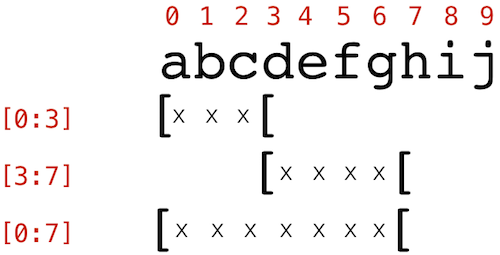
\includegraphics{media/brackets.png}
\caption{début et fin}
\end{figure}

    \begin{Verbatim}[commandchars=\\\{\}]
{\color{incolor}In [{\color{incolor}3}]:} \PY{c+c1}{\PYZsh{} chaine[a:b] + chaine[b:c] == chaine[a:c]}
        \PY{n}{chaine}\PY{p}{[}\PY{l+m+mi}{0}\PY{p}{:}\PY{l+m+mi}{3}\PY{p}{]} \PY{o}{+} \PY{n}{chaine}\PY{p}{[}\PY{l+m+mi}{3}\PY{p}{:}\PY{l+m+mi}{7}\PY{p}{]} \PY{o}{==} \PY{n}{chaine}\PY{p}{[}\PY{l+m+mi}{0}\PY{p}{:}\PY{l+m+mi}{7}\PY{p}{]}
\end{Verbatim}


\begin{Verbatim}[commandchars=\\\{\}]
{\color{outcolor}Out[{\color{outcolor}3}]:} True
\end{Verbatim}
            
    \hypertarget{bornes-omises}{%
\paragraph{Bornes omises}\label{bornes-omises}}

    On peut omettre une borne~:

    \begin{Verbatim}[commandchars=\\\{\}]
{\color{incolor}In [{\color{incolor}4}]:} \PY{c+c1}{\PYZsh{} si on omet la première borne, cela signifie que}
        \PY{c+c1}{\PYZsh{} la slice commence au début de l\PYZsq{}objet}
        \PY{n}{chaine}\PY{p}{[}\PY{p}{:}\PY{l+m+mi}{6}\PY{p}{]}
\end{Verbatim}


\begin{Verbatim}[commandchars=\\\{\}]
{\color{outcolor}Out[{\color{outcolor}4}]:} 'abcdef'
\end{Verbatim}
            
    \begin{Verbatim}[commandchars=\\\{\}]
{\color{incolor}In [{\color{incolor}5}]:} \PY{c+c1}{\PYZsh{} et bien entendu c\PYZsq{}est la même chose si on omet la deuxième borne}
        \PY{n}{chaine}\PY{p}{[}\PY{l+m+mi}{24}\PY{p}{:}\PY{p}{]}
\end{Verbatim}


\begin{Verbatim}[commandchars=\\\{\}]
{\color{outcolor}Out[{\color{outcolor}5}]:} 'yz'
\end{Verbatim}
            
    \begin{Verbatim}[commandchars=\\\{\}]
{\color{incolor}In [{\color{incolor}6}]:} \PY{c+c1}{\PYZsh{} ou même omettre les deux bornes, auquel cas on}
        \PY{c+c1}{\PYZsh{} fait une copie de l\PYZsq{}objet \PYZhy{} on y reviendra plus tard}
        \PY{n}{chaine}\PY{p}{[}\PY{p}{:}\PY{p}{]}
\end{Verbatim}


\begin{Verbatim}[commandchars=\\\{\}]
{\color{outcolor}Out[{\color{outcolor}6}]:} 'abcdefghijklmnopqrstuvwxyz'
\end{Verbatim}
            
    \hypertarget{indices-nuxe9gatifs}{%
\paragraph{Indices négatifs}\label{indices-nuxe9gatifs}}

    On peut utiliser des indices négatifs pour compter à partir de la fin~:

    \begin{Verbatim}[commandchars=\\\{\}]
{\color{incolor}In [{\color{incolor}7}]:} \PY{n}{chaine}\PY{p}{[}\PY{l+m+mi}{3}\PY{p}{:}\PY{o}{\PYZhy{}}\PY{l+m+mi}{3}\PY{p}{]}
\end{Verbatim}


\begin{Verbatim}[commandchars=\\\{\}]
{\color{outcolor}Out[{\color{outcolor}7}]:} 'defghijklmnopqrstuvw'
\end{Verbatim}
            
    \begin{Verbatim}[commandchars=\\\{\}]
{\color{incolor}In [{\color{incolor}8}]:} \PY{n}{chaine}\PY{p}{[}\PY{o}{\PYZhy{}}\PY{l+m+mi}{3}\PY{p}{:}\PY{p}{]}
\end{Verbatim}


\begin{Verbatim}[commandchars=\\\{\}]
{\color{outcolor}Out[{\color{outcolor}8}]:} 'xyz'
\end{Verbatim}
            
    \hypertarget{slice-avec-pas}{%
\subsubsection{Slice avec pas}\label{slice-avec-pas}}

    Il est également possible de préciser un \emph{pas}, de façon à ne
choisir par exemple, dans la plage donnée, qu'un élément sur deux~:

    \begin{Verbatim}[commandchars=\\\{\}]
{\color{incolor}In [{\color{incolor}9}]:} \PY{c+c1}{\PYZsh{} le pas est précisé après un deuxième deux\PYZhy{}points (:)}
        \PY{c+c1}{\PYZsh{} ici on va choisir un caractère sur deux dans la plage [3:\PYZhy{}3]}
        \PY{n}{chaine}\PY{p}{[}\PY{l+m+mi}{3}\PY{p}{:}\PY{o}{\PYZhy{}}\PY{l+m+mi}{3}\PY{p}{:}\PY{l+m+mi}{2}\PY{p}{]}
\end{Verbatim}


\begin{Verbatim}[commandchars=\\\{\}]
{\color{outcolor}Out[{\color{outcolor}9}]:} 'dfhjlnprtv'
\end{Verbatim}
            
    Comme on le devine, le troisième élément de la slice, ici \texttt{2},
détermine le pas. On ne retient donc, dans la chaîne \texttt{defghi...}
que \texttt{d}, puis \texttt{f}, et ainsi de suite.

On peut préciser du coup la borne de fin (ici \texttt{-3}) avec un peu
de liberté, puisqu'ici on obtiendrait un résultat identique avec
\texttt{-4}.

    \begin{Verbatim}[commandchars=\\\{\}]
{\color{incolor}In [{\color{incolor}10}]:} \PY{n}{chaine}\PY{p}{[}\PY{l+m+mi}{3}\PY{p}{:}\PY{o}{\PYZhy{}}\PY{l+m+mi}{4}\PY{p}{:}\PY{l+m+mi}{2}\PY{p}{]}
\end{Verbatim}


\begin{Verbatim}[commandchars=\\\{\}]
{\color{outcolor}Out[{\color{outcolor}10}]:} 'dfhjlnprtv'
\end{Verbatim}
            
    \hypertarget{pas-nuxe9gatif}{%
\subsubsection{Pas négatif}\label{pas-nuxe9gatif}}

    Il est même possible de spécifier un pas négatif. Dans ce cas, de
manière un peu contre-intuitive, il faut préciser un début (le premier
indice de la slice) qui soit \emph{plus à droite} que la fin (le second
indice).

Pour prendre un exemple, comme l'élément d'indice \texttt{-3},
c'est-à-dire \texttt{x}, est plus à droite que l'élément d'indice
\texttt{3}, c'est-à-dire \texttt{d}, évidemment si on ne précisait pas
le pas (qui revient à choisir un pas égal à \texttt{1}), on obtiendrait
une liste vide~:

    \begin{Verbatim}[commandchars=\\\{\}]
{\color{incolor}In [{\color{incolor}11}]:} \PY{n}{chaine}\PY{p}{[}\PY{o}{\PYZhy{}}\PY{l+m+mi}{3}\PY{p}{:}\PY{l+m+mi}{3}\PY{p}{]}
\end{Verbatim}


\begin{Verbatim}[commandchars=\\\{\}]
{\color{outcolor}Out[{\color{outcolor}11}]:} ''
\end{Verbatim}
            
    Si maintenant on précise un pas négatif, on obtient cette fois~:

    \begin{Verbatim}[commandchars=\\\{\}]
{\color{incolor}In [{\color{incolor}12}]:} \PY{n}{chaine}\PY{p}{[}\PY{o}{\PYZhy{}}\PY{l+m+mi}{3}\PY{p}{:}\PY{l+m+mi}{3}\PY{p}{:}\PY{o}{\PYZhy{}}\PY{l+m+mi}{2}\PY{p}{]}
\end{Verbatim}


\begin{Verbatim}[commandchars=\\\{\}]
{\color{outcolor}Out[{\color{outcolor}12}]:} 'xvtrpnljhf'
\end{Verbatim}
            
    \hypertarget{conclusion}{%
\subsubsection{Conclusion}\label{conclusion}}

    À nouveau, souvenez-vous que tous ces mécanismes fonctionnent avec de
nombreux autres types que les chaînes de caractères. En voici deux
exemples qui anticipent tous les deux sur la suite, mais qui devraient
illustrer les vastes possibilités qui sont offertes avec les slices.

    \hypertarget{listes}{%
\paragraph{Listes}\label{listes}}

    Par exemple sur les listes~:

    \begin{Verbatim}[commandchars=\\\{\}]
{\color{incolor}In [{\color{incolor}13}]:} \PY{n}{liste} \PY{o}{=} \PY{p}{[}\PY{l+m+mi}{0}\PY{p}{,} \PY{l+m+mi}{2}\PY{p}{,} \PY{l+m+mi}{4}\PY{p}{,} \PY{l+m+mi}{8}\PY{p}{,} \PY{l+m+mi}{16}\PY{p}{,} \PY{l+m+mi}{32}\PY{p}{,} \PY{l+m+mi}{64}\PY{p}{,} \PY{l+m+mi}{128}\PY{p}{]}
         \PY{n}{liste}
\end{Verbatim}


\begin{Verbatim}[commandchars=\\\{\}]
{\color{outcolor}Out[{\color{outcolor}13}]:} [0, 2, 4, 8, 16, 32, 64, 128]
\end{Verbatim}
            
    \begin{Verbatim}[commandchars=\\\{\}]
{\color{incolor}In [{\color{incolor}14}]:} \PY{n}{liste}\PY{p}{[}\PY{o}{\PYZhy{}}\PY{l+m+mi}{1}\PY{p}{:}\PY{l+m+mi}{1}\PY{p}{:}\PY{o}{\PYZhy{}}\PY{l+m+mi}{2}\PY{p}{]}
\end{Verbatim}


\begin{Verbatim}[commandchars=\\\{\}]
{\color{outcolor}Out[{\color{outcolor}14}]:} [128, 32, 8]
\end{Verbatim}
            
    Et même ceci, qui peut être déroutant. Nous reviendrons dessus.

    \begin{Verbatim}[commandchars=\\\{\}]
{\color{incolor}In [{\color{incolor}15}]:} \PY{n}{liste}\PY{p}{[}\PY{l+m+mi}{2}\PY{p}{:}\PY{l+m+mi}{4}\PY{p}{]} \PY{o}{=} \PY{p}{[}\PY{l+m+mi}{100}\PY{p}{,} \PY{l+m+mi}{200}\PY{p}{,} \PY{l+m+mi}{300}\PY{p}{,} \PY{l+m+mi}{400}\PY{p}{,} \PY{l+m+mi}{500}\PY{p}{]}
         \PY{n}{liste}
\end{Verbatim}


\begin{Verbatim}[commandchars=\\\{\}]
{\color{outcolor}Out[{\color{outcolor}15}]:} [0, 2, 100, 200, 300, 400, 500, 16, 32, 64, 128]
\end{Verbatim}
            
    \hypertarget{compluxe9ment---niveau-avancuxe9}{%
\subsection{Complément - niveau
avancé}\label{compluxe9ment---niveau-avancuxe9}}

    \hypertarget{numpy}{%
\paragraph{\texorpdfstring{\texttt{numpy}}{numpy}}\label{numpy}}

    La bibliothèque \texttt{numpy} permet de manipuler des tableaux ou des
matrices. En anticipant (beaucoup) sur son usage que nous reverrons bien
entendu en détail, voici un aperçu de ce que l'on peut faire avec des
slices sur des objets \texttt{numpy}~:

    \begin{Verbatim}[commandchars=\\\{\}]
{\color{incolor}In [{\color{incolor}16}]:} \PY{c+c1}{\PYZsh{} ces deux premières cellules sont à admettre}
         \PY{c+c1}{\PYZsh{} on construit un tableau ligne}
         \PY{k+kn}{import} \PY{n+nn}{numpy} \PY{k}{as} \PY{n+nn}{np}
         
         \PY{n}{un\PYZus{}cinq} \PY{o}{=} \PY{n}{np}\PY{o}{.}\PY{n}{array}\PY{p}{(}\PY{p}{[}\PY{l+m+mi}{1}\PY{p}{,} \PY{l+m+mi}{2}\PY{p}{,} \PY{l+m+mi}{3}\PY{p}{,} \PY{l+m+mi}{4}\PY{p}{,} \PY{l+m+mi}{5}\PY{p}{]}\PY{p}{)}
         \PY{n}{un\PYZus{}cinq}
\end{Verbatim}


\begin{Verbatim}[commandchars=\\\{\}]
{\color{outcolor}Out[{\color{outcolor}16}]:} array([1, 2, 3, 4, 5])
\end{Verbatim}
            
    \begin{Verbatim}[commandchars=\\\{\}]
{\color{incolor}In [{\color{incolor}17}]:} \PY{c+c1}{\PYZsh{} ces deux premières cellules sont à admettre}
         \PY{c+c1}{\PYZsh{} on le combine avec lui\PYZhy{}même \PYZhy{} et en utilisant une slice un peu magique}
         \PY{c+c1}{\PYZsh{} pour former un tableau carré 5x5}
         
         \PY{n}{array} \PY{o}{=} \PY{l+m+mi}{10} \PY{o}{*} \PY{n}{un\PYZus{}cinq}\PY{p}{[}\PY{p}{:}\PY{p}{,} \PY{n}{np}\PY{o}{.}\PY{n}{newaxis}\PY{p}{]} \PY{o}{+} \PY{n}{un\PYZus{}cinq}
         \PY{n}{array}
\end{Verbatim}


\begin{Verbatim}[commandchars=\\\{\}]
{\color{outcolor}Out[{\color{outcolor}17}]:} array([[11, 12, 13, 14, 15],
                [21, 22, 23, 24, 25],
                [31, 32, 33, 34, 35],
                [41, 42, 43, 44, 45],
                [51, 52, 53, 54, 55]])
\end{Verbatim}
            
    Sur ce tableau de taille 5x5, nous pouvons aussi faire du slicing et
extraire le sous-tableau 3x3 au centre~:

    \begin{Verbatim}[commandchars=\\\{\}]
{\color{incolor}In [{\color{incolor}18}]:} \PY{n}{centre} \PY{o}{=} \PY{n}{array}\PY{p}{[}\PY{l+m+mi}{1}\PY{p}{:}\PY{l+m+mi}{4}\PY{p}{,} \PY{l+m+mi}{1}\PY{p}{:}\PY{l+m+mi}{4}\PY{p}{]}
         \PY{n}{centre}
\end{Verbatim}


\begin{Verbatim}[commandchars=\\\{\}]
{\color{outcolor}Out[{\color{outcolor}18}]:} array([[22, 23, 24],
                [32, 33, 34],
                [42, 43, 44]])
\end{Verbatim}
            
    On peut bien sûr également utiliser un pas~:

    \begin{Verbatim}[commandchars=\\\{\}]
{\color{incolor}In [{\color{incolor}19}]:} \PY{n}{coins} \PY{o}{=} \PY{n}{array}\PY{p}{[}\PY{p}{:}\PY{p}{:}\PY{l+m+mi}{4}\PY{p}{,} \PY{p}{:}\PY{p}{:}\PY{l+m+mi}{4}\PY{p}{]}
         \PY{n}{coins}
\end{Verbatim}


\begin{Verbatim}[commandchars=\\\{\}]
{\color{outcolor}Out[{\color{outcolor}19}]:} array([[11, 15],
                [51, 55]])
\end{Verbatim}
            
    Ou bien retourner complètement dans une direction~:

    \begin{Verbatim}[commandchars=\\\{\}]
{\color{incolor}In [{\color{incolor}20}]:} \PY{n}{tete\PYZus{}en\PYZus{}bas} \PY{o}{=} \PY{n}{array}\PY{p}{[}\PY{p}{:}\PY{p}{:}\PY{o}{\PYZhy{}}\PY{l+m+mi}{1}\PY{p}{,}\PY{p}{:}\PY{p}{]}
         \PY{n}{tete\PYZus{}en\PYZus{}bas}
\end{Verbatim}


\begin{Verbatim}[commandchars=\\\{\}]
{\color{outcolor}Out[{\color{outcolor}20}]:} array([[51, 52, 53, 54, 55],
                [41, 42, 43, 44, 45],
                [31, 32, 33, 34, 35],
                [21, 22, 23, 24, 25],
                [11, 12, 13, 14, 15]])
\end{Verbatim}
            

    % Add a bibliography block to the postdoc
    
    
    

        \hypertarget{muxe9thodes-spuxe9cifiques-aux-listes}{%
\section{Méthodes spécifiques aux
listes}\label{muxe9thodes-spuxe9cifiques-aux-listes}}

    \hypertarget{compluxe9ment---niveau-basique}{%
\subsection{Complément - niveau
basique}\label{compluxe9ment---niveau-basique}}

    Voici quelques unes des méthodes disponibles sur le type \texttt{list}.

    \hypertarget{trouver-linformation}{%
\subsubsection{Trouver l'information}\label{trouver-linformation}}

    Pour commencer, rappelons comment retrouver la liste des méthodes
définies sur le type \texttt{list}~:

    \begin{Verbatim}[commandchars=\\\{\}]
{\color{incolor}In [{\color{incolor}1}]:} \PY{n}{help}\PY{p}{(}\PY{n+nb}{list}\PY{p}{)}
\end{Verbatim}


    \begin{Verbatim}[commandchars=\\\{\}]
Help on class list in module builtins:

class list(object)
 |  list() -> new empty list
 |  list(iterable) -> new list initialized from iterable's items
 |  
 |  Methods defined here:
 |  
 |  \_\_add\_\_(self, value, /)
 |      Return self+value.
 |  
 |  \_\_contains\_\_(self, key, /)
 |      Return key in self.
 |  
 |  \_\_delitem\_\_(self, key, /)
 |      Delete self[key].
 |  
 |  \_\_eq\_\_(self, value, /)
 |      Return self==value.
 |  
 |  \_\_ge\_\_(self, value, /)
 |      Return self>=value.
 |  
 |  \_\_getattribute\_\_(self, name, /)
 |      Return getattr(self, name).
 |  
 |  \_\_getitem\_\_({\ldots})
 |      x.\_\_getitem\_\_(y) <==> x[y]
 |  
 |  \_\_gt\_\_(self, value, /)
 |      Return self>value.
 |  
 |  \_\_iadd\_\_(self, value, /)
 |      Implement self+=value.
 |  
 |  \_\_imul\_\_(self, value, /)
 |      Implement self*=value.
 |  
 |  \_\_init\_\_(self, /, *args, **kwargs)
 |      Initialize self.  See help(type(self)) for accurate signature.
 |  
 |  \_\_iter\_\_(self, /)
 |      Implement iter(self).
 |  
 |  \_\_le\_\_(self, value, /)
 |      Return self<=value.
 |  
 |  \_\_len\_\_(self, /)
 |      Return len(self).
 |  
 |  \_\_lt\_\_(self, value, /)
 |      Return self<value.
 |  
 |  \_\_mul\_\_(self, value, /)
 |      Return self*value.n
 |  
 |  \_\_ne\_\_(self, value, /)
 |      Return self!=value.
 |  
 |  \_\_new\_\_(*args, **kwargs) from builtins.type
 |      Create and return a new object.  See help(type) for accurate signature.
 |  
 |  \_\_repr\_\_(self, /)
 |      Return repr(self).
 |  
 |  \_\_reversed\_\_({\ldots})
 |      L.\_\_reversed\_\_() -- return a reverse iterator over the list
 |  
 |  \_\_rmul\_\_(self, value, /)
 |      Return self*value.
 |  
 |  \_\_setitem\_\_(self, key, value, /)
 |      Set self[key] to value.
 |  
 |  \_\_sizeof\_\_({\ldots})
 |      L.\_\_sizeof\_\_() -- size of L in memory, in bytes
 |  
 |  append({\ldots})
 |      L.append(object) -> None -- append object to end
 |  
 |  clear({\ldots})
 |      L.clear() -> None -- remove all items from L
 |  
 |  copy({\ldots})
 |      L.copy() -> list -- a shallow copy of L
 |  
 |  count({\ldots})
 |      L.count(value) -> integer -- return number of occurrences of value
 |  
 |  extend({\ldots})
 |      L.extend(iterable) -> None -- extend list by appending elements from the iterable
 |  
 |  index({\ldots})
 |      L.index(value, [start, [stop]]) -> integer -- return first index of value.
 |      Raises ValueError if the value is not present.
 |  
 |  insert({\ldots})
 |      L.insert(index, object) -- insert object before index
 |  
 |  pop({\ldots})
 |      L.pop([index]) -> item -- remove and return item at index (default last).
 |      Raises IndexError if list is empty or index is out of range.
 |  
 |  remove({\ldots})
 |      L.remove(value) -> None -- remove first occurrence of value.
 |      Raises ValueError if the value is not present.
 |  
 |  reverse({\ldots})
 |      L.reverse() -- reverse *IN PLACE*
 |  
 |  sort({\ldots})
 |      L.sort(key=None, reverse=False) -> None -- stable sort *IN PLACE*
 |  
 |  ----------------------------------------------------------------------
 |  Data and other attributes defined here:
 |  
 |  \_\_hash\_\_ = None


    \end{Verbatim}

    Ignorez les méthodes dont le nom commence et termine par \texttt{\_\_}
(nous parlerons de ceci en semaine 6), vous trouvez alors les méthodes
utiles listées entre \texttt{append} et \texttt{sort}.\\

Certaines de ces méthodes ont été vues dans la vidéo sur les séquences,
c'est le cas notamment de \texttt{count} et \texttt{index}.\\

    Nous allons à présent décrire les autres, partiellement et brièvement.
Un autre complément décrit la méthode \texttt{sort}. Reportez-vous au
lien donné en fin de notebook pour obtenir une information plus
complète.\\

    Donnons-nous pour commencer une liste témoin~:

    \begin{Verbatim}[commandchars=\\\{\}]
{\color{incolor}In [{\color{incolor}2}]:} \PY{n}{liste} \PY{o}{=} \PY{p}{[}\PY{l+m+mi}{0}\PY{p}{,} \PY{l+m+mi}{1}\PY{p}{,} \PY{l+m+mi}{2}\PY{p}{,} \PY{l+m+mi}{3}\PY{p}{]}
        \PY{n+nb}{print}\PY{p}{(}\PY{l+s+s1}{\PYZsq{}}\PY{l+s+s1}{liste}\PY{l+s+s1}{\PYZsq{}}\PY{p}{,} \PY{n}{liste}\PY{p}{)}
\end{Verbatim}


    \begin{Verbatim}[commandchars=\\\{\}]
liste [0, 1, 2, 3]

    \end{Verbatim}

    \textbf{Avertissements}~:

\begin{itemize}
\tightlist
\item
  soyez bien attentifs au nombre de fois où vous exécutez les cellules
  de ce notebook~;
\item
  par exemple une liste renversée deux fois peut donner l'impression que
  \texttt{reverse} ne marche pas~;
\item
  n'hésitez pas à utiliser le menu \emph{Cell~-\textgreater{}~Run~All}
  pour réexécuter en une seule fois le notebook entier.
\end{itemize}

    \hypertarget{append}{%
\subsubsection{\texorpdfstring{\textbf{append}}{append}}\label{append}}

    La méthode \texttt{append} permet d'ajouter \textbf{un élément} à la fin
d'une liste~:

    \begin{Verbatim}[commandchars=\\\{\}]
{\color{incolor}In [{\color{incolor}3}]:} \PY{n}{liste}\PY{o}{.}\PY{n}{append}\PY{p}{(}\PY{l+s+s1}{\PYZsq{}}\PY{l+s+s1}{ap}\PY{l+s+s1}{\PYZsq{}}\PY{p}{)}
        \PY{n+nb}{print}\PY{p}{(}\PY{l+s+s1}{\PYZsq{}}\PY{l+s+s1}{liste}\PY{l+s+s1}{\PYZsq{}}\PY{p}{,} \PY{n}{liste}\PY{p}{)}
\end{Verbatim}


    \begin{Verbatim}[commandchars=\\\{\}]
liste [0, 1, 2, 3, 'ap']

    \end{Verbatim}

    \hypertarget{extend}{%
\subsubsection{\texorpdfstring{\textbf{extend}}{extend}}\label{extend}}

    La méthode \texttt{extend} réalise la même opération, mais avec
\textbf{tous les éléments} de la liste qu'on lui passe en argument~:

    \begin{Verbatim}[commandchars=\\\{\}]
{\color{incolor}In [{\color{incolor}4}]:} \PY{n}{liste2} \PY{o}{=} \PY{p}{[}\PY{l+s+s1}{\PYZsq{}}\PY{l+s+s1}{ex1}\PY{l+s+s1}{\PYZsq{}}\PY{p}{,} \PY{l+s+s1}{\PYZsq{}}\PY{l+s+s1}{ex2}\PY{l+s+s1}{\PYZsq{}}\PY{p}{]}
        \PY{n}{liste}\PY{o}{.}\PY{n}{extend}\PY{p}{(}\PY{n}{liste2}\PY{p}{)}
        \PY{n+nb}{print}\PY{p}{(}\PY{l+s+s1}{\PYZsq{}}\PY{l+s+s1}{liste}\PY{l+s+s1}{\PYZsq{}}\PY{p}{,} \PY{n}{liste}\PY{p}{)}
\end{Verbatim}


    \begin{Verbatim}[commandchars=\\\{\}]
liste [0, 1, 2, 3, 'ap', 'ex1', 'ex2']

    \end{Verbatim}

    \hypertarget{append-vs}{%
\subsubsection{\texorpdfstring{\textbf{append} \emph{vs}
\textbf{+}}{append vs +}}\label{append-vs}}

    Ces deux méthodes \texttt{append} et \texttt{extend} sont donc assez
voisines~; avant de voir d'autres méthodes de \texttt{list}, prenons un
peu le temps de comparer leur comportement avec l'addition \texttt{+} de
liste. L'élément clé ici, on l'a déjà vu dans la vidéo, est que la liste
est un objet \textbf{mutable}. \texttt{append} et \texttt{extend}
\textbf{modifient} la liste sur laquelle elles travaillent, alors que
l'addition \textbf{crée un nouvel objet}.

    \begin{Verbatim}[commandchars=\\\{\}]
{\color{incolor}In [{\color{incolor}5}]:} \PY{c+c1}{\PYZsh{} pour créer une liste avec les n premiers entiers, on utilise}
        \PY{c+c1}{\PYZsh{} la fonction built\PYZhy{}in range(), que l\PYZsq{}on convertit en liste}
        \PY{c+c1}{\PYZsh{} on aura l\PYZsq{}occasion d\PYZsq{}y revenir}
        \PY{n}{a1} \PY{o}{=} \PY{n+nb}{list}\PY{p}{(}\PY{n+nb}{range}\PY{p}{(}\PY{l+m+mi}{3}\PY{p}{)}\PY{p}{)}
        \PY{n+nb}{print}\PY{p}{(}\PY{n}{a1}\PY{p}{)}
\end{Verbatim}


    \begin{Verbatim}[commandchars=\\\{\}]
[0, 1, 2]

    \end{Verbatim}

    \begin{Verbatim}[commandchars=\\\{\}]
{\color{incolor}In [{\color{incolor}6}]:} \PY{n}{a2} \PY{o}{=} \PY{n+nb}{list}\PY{p}{(}\PY{n+nb}{range}\PY{p}{(}\PY{l+m+mi}{10}\PY{p}{,} \PY{l+m+mi}{13}\PY{p}{)}\PY{p}{)}
        \PY{n+nb}{print}\PY{p}{(}\PY{n}{a2}\PY{p}{)}
\end{Verbatim}


    \begin{Verbatim}[commandchars=\\\{\}]
[10, 11, 12]

    \end{Verbatim}

    \begin{Verbatim}[commandchars=\\\{\}]
{\color{incolor}In [{\color{incolor}7}]:} \PY{c+c1}{\PYZsh{} le fait d\PYZsq{}utiliser + crée une nouvelle liste}
        \PY{n}{a3} \PY{o}{=} \PY{n}{a1} \PY{o}{+} \PY{n}{a2}
\end{Verbatim}


    \begin{Verbatim}[commandchars=\\\{\}]
{\color{incolor}In [{\color{incolor}8}]:} \PY{c+c1}{\PYZsh{} si bien que maintenant on a trois objets différents}
        \PY{n+nb}{print}\PY{p}{(}\PY{l+s+s1}{\PYZsq{}}\PY{l+s+s1}{a1}\PY{l+s+s1}{\PYZsq{}}\PY{p}{,} \PY{n}{a1}\PY{p}{)}
        \PY{n+nb}{print}\PY{p}{(}\PY{l+s+s1}{\PYZsq{}}\PY{l+s+s1}{a2}\PY{l+s+s1}{\PYZsq{}}\PY{p}{,} \PY{n}{a2}\PY{p}{)}
        \PY{n+nb}{print}\PY{p}{(}\PY{l+s+s1}{\PYZsq{}}\PY{l+s+s1}{a3}\PY{l+s+s1}{\PYZsq{}}\PY{p}{,} \PY{n}{a3}\PY{p}{)}
\end{Verbatim}


    \begin{Verbatim}[commandchars=\\\{\}]
a1 [0, 1, 2]
a2 [10, 11, 12]
a3 [0, 1, 2, 10, 11, 12]

    \end{Verbatim}

    Comme on le voit, après une addition, les deux termes de l'addition sont
inchangés. Pour bien comprendre, voyons exactement le même scénario sous
pythontutor~:

    \begin{Verbatim}[commandchars=\\\{\}]
{\color{incolor}In [{\color{incolor} }]:} \PY{o}{\PYZpc{}}\PY{k}{load\PYZus{}ext} ipythontutor
\end{Verbatim}


    \textbf{Note}~: une fois que vous avez évalué la cellule avec
\texttt{\%\%ipythontutor}, vous devez cliquer sur le bouton
\texttt{Forward} pour voir pas à pas le comportement du programme.

    \begin{Verbatim}[commandchars=\\\{\}]
{\color{incolor}In [{\color{incolor} }]:} \PY{o}{\PYZpc{}\PYZpc{}}\PY{k}{ipythontutor} height=230 ratio=0.7
        a1 = list(range(3))
        a2 = list(range(10, 13))
        a3 = a1 + a2
\end{Verbatim}


    Alors que si on avait utilisé \texttt{extend}, on aurait obtenu ceci~:

    \begin{Verbatim}[commandchars=\\\{\}]
{\color{incolor}In [{\color{incolor} }]:} \PY{o}{\PYZpc{}\PYZpc{}}\PY{k}{ipythontutor} height=200 ratio=0.75
        e1 = list(range(3))
        e2 = list(range(10, 13))
        e3 = e1.extend(e2)
\end{Verbatim}


    Ici on tire profit du fait que la liste est un objet mutable~:
\texttt{extend} \textbf{modifie} l'objet sur lequel on l'appelle (ici
\texttt{e1}). Dans ce scénario on ne crée en tout que deux objets, et du
coup il est inutile pour extend de renvoyer quoi que ce soit, et c'est
pourquoi \texttt{e3} ici vaut None.\\

    C'est pour cette raison que~:

\begin{itemize}
\tightlist
\item
  l'addition est disponible sur tous les types séquences - on peut
  toujours réaliser l'addition puisqu'on crée un nouvel objet pour
  stocker le résultat de l'addition~;
\item
  mais \texttt{append} et \texttt{extend} ne sont par exemple
  \textbf{pas disponibles} sur les chaînes de caractères, qui sont
  \textbf{immuables} - si \texttt{e1} était une chaîne, on ne pourrait
  pas la modifier pour lui ajouter des éléments.
\end{itemize}

    \hypertarget{insert}{%
\subsubsection{\texorpdfstring{\textbf{insert}}{insert}}\label{insert}}

    Reprenons notre inventaire des méthodes de \texttt{list}, et pour cela
rappelons nous le contenu de la variable \texttt{liste}~:

    \begin{Verbatim}[commandchars=\\\{\}]
{\color{incolor}In [{\color{incolor}9}]:} \PY{n}{liste}
\end{Verbatim}


\begin{Verbatim}[commandchars=\\\{\}]
{\color{outcolor}Out[{\color{outcolor}9}]:} [0, 1, 2, 3, 'ap', 'ex1', 'ex2']
\end{Verbatim}
            
    La méthode \texttt{insert} permet, comme le nom le suggère, d'insérer un
élément à une certaine position~; comme toujours les indices commencent
à zéro et donc~:

    \begin{Verbatim}[commandchars=\\\{\}]
{\color{incolor}In [{\color{incolor}10}]:} \PY{c+c1}{\PYZsh{} insérer à l\PYZsq{}index 2}
         \PY{n}{liste}\PY{o}{.}\PY{n}{insert}\PY{p}{(}\PY{l+m+mi}{2}\PY{p}{,} \PY{l+s+s1}{\PYZsq{}}\PY{l+s+s1}{1 bis}\PY{l+s+s1}{\PYZsq{}}\PY{p}{)}
         \PY{n+nb}{print}\PY{p}{(}\PY{l+s+s1}{\PYZsq{}}\PY{l+s+s1}{liste}\PY{l+s+s1}{\PYZsq{}}\PY{p}{,} \PY{n}{liste}\PY{p}{)}
\end{Verbatim}


    \begin{Verbatim}[commandchars=\\\{\}]
liste [0, 1, '1 bis', 2, 3, 'ap', 'ex1', 'ex2']

    \end{Verbatim}

    On peut remarquer qu'un résultat analogue peut être obtenu avec une
affectation de slice~; par exemple pour insérer au rang 5 (i.e.~avant
\texttt{ap}), on pourrait aussi bien faire~:

    \begin{Verbatim}[commandchars=\\\{\}]
{\color{incolor}In [{\color{incolor}11}]:} \PY{n}{liste}\PY{p}{[}\PY{l+m+mi}{5}\PY{p}{:}\PY{l+m+mi}{5}\PY{p}{]} \PY{o}{=} \PY{p}{[}\PY{l+s+s1}{\PYZsq{}}\PY{l+s+s1}{3 bis}\PY{l+s+s1}{\PYZsq{}}\PY{p}{]}
         \PY{n+nb}{print}\PY{p}{(}\PY{l+s+s1}{\PYZsq{}}\PY{l+s+s1}{liste}\PY{l+s+s1}{\PYZsq{}}\PY{p}{,} \PY{n}{liste}\PY{p}{)}
\end{Verbatim}


    \begin{Verbatim}[commandchars=\\\{\}]
liste [0, 1, '1 bis', 2, 3, '3 bis', 'ap', 'ex1', 'ex2']

    \end{Verbatim}

    \hypertarget{remove}{%
\subsubsection{\texorpdfstring{\textbf{remove}}{remove}}\label{remove}}

    La méthode \texttt{remove} détruit la \textbf{première occurrence} d'un
objet dans la liste~:

    \begin{Verbatim}[commandchars=\\\{\}]
{\color{incolor}In [{\color{incolor}12}]:} \PY{n}{liste}\PY{o}{.}\PY{n}{remove}\PY{p}{(}\PY{l+m+mi}{3}\PY{p}{)}
         \PY{n+nb}{print}\PY{p}{(}\PY{l+s+s1}{\PYZsq{}}\PY{l+s+s1}{liste}\PY{l+s+s1}{\PYZsq{}}\PY{p}{,} \PY{n}{liste}\PY{p}{)}
\end{Verbatim}


    \begin{Verbatim}[commandchars=\\\{\}]
liste [0, 1, '1 bis', 2, '3 bis', 'ap', 'ex1', 'ex2']

    \end{Verbatim}

    \hypertarget{pop}{%
\subsubsection{\texorpdfstring{\textbf{pop}}{pop}}\label{pop}}

    La méthode \texttt{pop} prend en argument un indice~; elle permet
d'extraire l'élément à cet indice. En un seul appel on obtient la valeur
de l'élément et on l'enlève de la liste~:

    \begin{Verbatim}[commandchars=\\\{\}]
{\color{incolor}In [{\color{incolor}13}]:} \PY{n}{popped} \PY{o}{=} \PY{n}{liste}\PY{o}{.}\PY{n}{pop}\PY{p}{(}\PY{l+m+mi}{0}\PY{p}{)}
         \PY{n+nb}{print}\PY{p}{(}\PY{l+s+s1}{\PYZsq{}}\PY{l+s+s1}{popped}\PY{l+s+s1}{\PYZsq{}}\PY{p}{,} \PY{n}{popped}\PY{p}{,} \PY{l+s+s1}{\PYZsq{}}\PY{l+s+s1}{liste}\PY{l+s+s1}{\PYZsq{}}\PY{p}{,} \PY{n}{liste}\PY{p}{)}
\end{Verbatim}


    \begin{Verbatim}[commandchars=\\\{\}]
popped 0 liste [1, '1 bis', 2, '3 bis', 'ap', 'ex1', 'ex2']

    \end{Verbatim}

    Si l'indice n'est pas précisé, c'est le dernier élément de la liste qui
est visé~:

    \begin{Verbatim}[commandchars=\\\{\}]
{\color{incolor}In [{\color{incolor}14}]:} \PY{n}{popped} \PY{o}{=} \PY{n}{liste}\PY{o}{.}\PY{n}{pop}\PY{p}{(}\PY{p}{)}
         \PY{n+nb}{print}\PY{p}{(}\PY{l+s+s1}{\PYZsq{}}\PY{l+s+s1}{popped}\PY{l+s+s1}{\PYZsq{}}\PY{p}{,} \PY{n}{popped}\PY{p}{,} \PY{l+s+s1}{\PYZsq{}}\PY{l+s+s1}{liste}\PY{l+s+s1}{\PYZsq{}}\PY{p}{,} \PY{n}{liste}\PY{p}{)}
\end{Verbatim}


    \begin{Verbatim}[commandchars=\\\{\}]
popped ex2 liste [1, '1 bis', 2, '3 bis', 'ap', 'ex1']

    \end{Verbatim}

    \hypertarget{reverse}{%
\subsubsection{\texorpdfstring{\textbf{reverse}}{reverse}}\label{reverse}}

    Enfin \texttt{reverse} renverse la liste, le premier élément devient le
dernier~:

    \begin{Verbatim}[commandchars=\\\{\}]
{\color{incolor}In [{\color{incolor}15}]:} \PY{n}{liste}\PY{o}{.}\PY{n}{reverse}\PY{p}{(}\PY{p}{)}
         \PY{n+nb}{print}\PY{p}{(}\PY{l+s+s1}{\PYZsq{}}\PY{l+s+s1}{liste}\PY{l+s+s1}{\PYZsq{}}\PY{p}{,} \PY{n}{liste}\PY{p}{)}
\end{Verbatim}


    \begin{Verbatim}[commandchars=\\\{\}]
liste ['ex1', 'ap', '3 bis', 2, '1 bis', 1]

    \end{Verbatim}

    On peut remarquer ici que le résultat se rapproche de ce qu'on peut
obtenir avec une opération de slicing comme ceci~:

    \begin{Verbatim}[commandchars=\\\{\}]
{\color{incolor}In [{\color{incolor}16}]:} \PY{n}{liste2} \PY{o}{=} \PY{n}{liste}\PY{p}{[}\PY{p}{:}\PY{p}{:}\PY{o}{\PYZhy{}}\PY{l+m+mi}{1}\PY{p}{]}
         \PY{n+nb}{print}\PY{p}{(}\PY{l+s+s1}{\PYZsq{}}\PY{l+s+s1}{liste2}\PY{l+s+s1}{\PYZsq{}}\PY{p}{,} \PY{n}{liste2}\PY{p}{)}
\end{Verbatim}


    \begin{Verbatim}[commandchars=\\\{\}]
liste2 [1, '1 bis', 2, '3 bis', 'ap', 'ex1']

    \end{Verbatim}

    \textbf{À la différence toutefois} qu'avec le slicing c'est une copie de
la liste initiale qui est retournée, la liste de départ quant à elle
n'est pas modifiée.

    \hypertarget{pour-en-savoir-plus}{%
\subsubsection{Pour en savoir plus}\label{pour-en-savoir-plus}}

    \href{https://docs.python.org/3/tutorial/datastructures.html\#more-on-lists}{https://docs.python.org/3/tutorial/datastructures.html\#more-on-lists}

    \hypertarget{note-spuxe9cifique-aux-notebooks}{%
\subsubsection{Note spécifique aux
notebooks}\label{note-spuxe9cifique-aux-notebooks}}

    \hypertarget{help-avec}{%
\paragraph{\texorpdfstring{\texttt{help} avec
\texttt{?}}{help avec ?}}\label{help-avec}}

    Je vous signale en passant que dans un notebook vous pouvez obtenir de
l'aide avec un point d'interrogation \texttt{?} inséré avant ou après un
symbole. Par exemple pour obtenir des précisions sur la méthode
\texttt{list.pop}, on peut faire soit~:

    \begin{Verbatim}[commandchars=\\\{\}]
{\color{incolor}In [{\color{incolor}17}]:} \PY{c+c1}{\PYZsh{} fonctionne dans tous les environnements Python}
         \PY{n}{help}\PY{p}{(}\PY{n+nb}{list}\PY{o}{.}\PY{n}{pop}\PY{p}{)}
\end{Verbatim}


    \begin{Verbatim}[commandchars=\\\{\}]
Help on method\_descriptor:

pop({\ldots})
    L.pop([index]) -> item -- remove and return item at index (default last).
    Raises IndexError if list is empty or index is out of range.


    \end{Verbatim}

    \begin{Verbatim}[commandchars=\\\{\}]
{\color{incolor}In [{\color{incolor}18}]:} \PY{c+c1}{\PYZsh{} spécifique aux notebooks}
         \PY{c+c1}{\PYZsh{} l\PYZsq{}affichage obtenu est légèrement différent}
         \PY{c+c1}{\PYZsh{} tapez la touche \PYZsq{}Esc\PYZsq{} \PYZhy{} ou cliquez la petite croix}
         \PY{c+c1}{\PYZsh{} pour faire disparaitre le dialogue qui apparaît en bas}
         list.pop\PY{o}{?}
\end{Verbatim}


    \hypertarget{compluxe9tion-avec-tab}{%
\paragraph{\texorpdfstring{Complétion avec
\texttt{Tab}}{Complétion avec Tab}\\\\}\label{compluxe9tion-avec-tab}}

    Dans un notebook vous avez aussi la complétion~; si vous tapez - dans
une cellule de code - le début d'un symbole connu dans l'environnement~:

    \begin{Verbatim}[commandchars=\\\{\}]
{\color{incolor}In [{\color{incolor} }]:} \PY{c+c1}{\PYZsh{} placez votre curseur à la fin de la ligne après \PYZsq{}li\PYZsq{}}
        \PY{c+c1}{\PYZsh{} et appuyez sur la touche \PYZsq{}Tab\PYZsq{}}
        \PY{n}{li}
\end{Verbatim}


    Vous voyez apparaître un dialogue avec les noms connus qui commencent
par \texttt{li}~; utilisez les flèches pour choisir, et `Return' pour
sélectionner.
        
    
    
    

    

    \hypertarget{objets-mutables-et-objets-immuables}{%
\section{Objets mutables et objets
immuables}\label{objets-mutables-et-objets-immuables}}

    \hypertarget{compluxe9ment---niveau-basique}{%
\subsection{Complément - niveau
basique}\label{compluxe9ment---niveau-basique}}

    \hypertarget{les-chauxeenes-sont-des-objets-immuables}{%
\subsubsection{Les chaînes sont des objets
immuables}\label{les-chauxeenes-sont-des-objets-immuables}}

    Voici un exemple d'un fragment de code qui illustre le caractère
immuable des chaînes de caractères. Nous l'exécutons sous
\href{pythontutor.com}{pythontutor}, afin de bien illustrer les
relations entre variables et objets.

    \begin{Verbatim}[commandchars=\\\{\},frame=single,framerule=0.3mm,rulecolor=\color{cellframecolor}]
{\color{incolor}In [{\color{incolor}1}]:} \PY{c+c1}{\PYZsh{} il vous faut charger cette cellule}
        \PY{c+c1}{\PYZsh{} pour pouvoir utiliser les suivantes}
        \PY{o}{\PYZpc{}}\PY{k}{load\PYZus{}ext} ipythontutor
\end{Verbatim}


    \textbf{Note}~: une fois que vous avez évalué la cellule avec
\texttt{\%\%ipythontutor}, vous devez cliquer sur le bouton
\texttt{Forward} pour voir pas à pas le comportement du programme.

    Le scénario est très simple, on crée deux variables \texttt{s1} et
\texttt{s2} vers le même objet
\texttt{\textquotesingle{}abc\textquotesingle{}}, puis on fait une
opération \texttt{+=} sur la variable \texttt{s1}.

Comme l'objet est une chaîne, il est donc immuable, on ne \textbf{peut
pas modifier l'objet} directement~; pour obtenir l'effet recherché (à
savoir que \texttt{s1} s'allonge de
\texttt{\textquotesingle{}def\textquotesingle{}}), Python \textbf{crée
un deuxième objet}, comme on le voit bien sous pythontutor~:

    \begin{Verbatim}[commandchars=\\\{\},frame=single,framerule=0.3mm,rulecolor=\color{cellframecolor}]
{\color{incolor}In [{\color{incolor} }]:} \PY{c+c1}{\PYZsh{} NOTE}
        \PY{c+c1}{\PYZsh{} auto\PYZhy{}exec\PYZhy{}for\PYZhy{}latex has skipped execution of this cell}
        
        \PY{o}{\PYZpc{}\PYZpc{}}\PY{k}{ipythontutor} heapPrimitives=true
        \PYZsh{} deux variables vers le même objet
        s1 = \PYZsq{}abc\PYZsq{}
        s2 = s1
        \PYZsh{} on essaie de modifier l\PYZsq{}objet
        s1 += \PYZsq{}def\PYZsq{}
        \PYZsh{} pensez à cliquer sur `Forward`
\end{Verbatim}


    \hypertarget{les-listes-sont-des-objets-mutables}{%
\subsubsection{Les listes sont des objets
mutables}\label{les-listes-sont-des-objets-mutables}}

    Voici ce qu'on obtient par contraste pour le même scénario mais qui
cette fois utilise des listes, qui sont des objets mutables~:

    \begin{Verbatim}[commandchars=\\\{\},frame=single,framerule=0.3mm,rulecolor=\color{cellframecolor}]
{\color{incolor}In [{\color{incolor} }]:} \PY{c+c1}{\PYZsh{} NOTE}
        \PY{c+c1}{\PYZsh{} auto\PYZhy{}exec\PYZhy{}for\PYZhy{}latex has skipped execution of this cell}
        
        \PY{o}{\PYZpc{}\PYZpc{}}\PY{k}{ipythontutor} heapPrimitives=true ratio=0.8
        \PYZsh{} deux variables vers le même objet
        liste1 = [\PYZsq{}a\PYZsq{}, \PYZsq{}b\PYZsq{}, \PYZsq{}c\PYZsq{}]
        liste2 = liste1
        \PYZsh{} on modifie l\PYZsq{}objet
        liste1 += [\PYZsq{}d\PYZsq{}, \PYZsq{}e\PYZsq{}, \PYZsq{}f\PYZsq{}]
        \PYZsh{} pensez à cliquer sur `Forward`
\end{Verbatim}


    \hypertarget{conclusion}{%
\subsubsection{Conclusion}\label{conclusion}}

    Ce comportement n'est pas propre à l'usage de l'opérateur \texttt{+=} et
pour cette raison nous avons tendance à le déconseiller.

Les objets mutables et immuables ont par essence un comportement
différent, il est très important d'avoir ceci présent à l'esprit.

Nous aurons notamment l'occasion d'approfondir cela dans la séquence
consacrée aux références partagées, en semaine 3.


    % Add a bibliography block to the postdoc
    
    
    

        
    
    
    

    

    \hypertarget{tris-de-listes}{%
\section{Tris de listes}\label{tris-de-listes}}

    \hypertarget{compluxe9ment---niveau-basique}{%
\subsection{Complément - niveau
basique}\label{compluxe9ment---niveau-basique}}

    Python fournit une méthode standard pour trier une liste, qui s'appelle,
sans grande surprise, \texttt{sort}.

    \hypertarget{la-muxe9thode-sort}{%
\subsubsection{\texorpdfstring{La méthode
\texttt{sort}}{La méthode sort}}\label{la-muxe9thode-sort}}

    Voyons comment se comporte \texttt{sort} sur un exemple simple~:

    \begin{Verbatim}[commandchars=\\\{\}]
{\color{incolor}In [{\color{incolor}1}]:} \PY{n}{liste} \PY{o}{=} \PY{p}{[}\PY{l+m+mi}{8}\PY{p}{,} \PY{l+m+mi}{7}\PY{p}{,} \PY{l+m+mi}{4}\PY{p}{,} \PY{l+m+mi}{3}\PY{p}{,} \PY{l+m+mi}{2}\PY{p}{,} \PY{l+m+mi}{9}\PY{p}{,} \PY{l+m+mi}{1}\PY{p}{,} \PY{l+m+mi}{5}\PY{p}{,} \PY{l+m+mi}{6}\PY{p}{]}
        \PY{n+nb}{print}\PY{p}{(}\PY{l+s+s1}{\PYZsq{}}\PY{l+s+s1}{avant tri}\PY{l+s+s1}{\PYZsq{}}\PY{p}{,} \PY{n}{liste}\PY{p}{)}
        \PY{n}{liste}\PY{o}{.}\PY{n}{sort}\PY{p}{(}\PY{p}{)}
        \PY{n+nb}{print}\PY{p}{(}\PY{l+s+s1}{\PYZsq{}}\PY{l+s+s1}{apres tri}\PY{l+s+s1}{\PYZsq{}}\PY{p}{,} \PY{n}{liste}\PY{p}{)}
\end{Verbatim}


    \begin{Verbatim}[commandchars=\\\{\}]
avant tri [8, 7, 4, 3, 2, 9, 1, 5, 6]
apres tri [1, 2, 3, 4, 5, 6, 7, 8, 9]

    \end{Verbatim}

    On retrouve ici, avec l'instruction \texttt{liste.sort()} un cas d'appel
de méthode (ici \texttt{sort}) sur un objet (ici \texttt{liste}), comme
on l'avait vu dans la vidéo.

    La première chose à remarquer est que la liste d'entrée a été modifiée,
on dit ``en place'', ou encore ``par effet de bord''. Voyons cela sous
pythontutor~:

    \begin{Verbatim}[commandchars=\\\{\}]
{\color{incolor}In [{\color{incolor}2}]:} \PY{o}{\PYZpc{}}\PY{k}{load\PYZus{}ext} ipythontutor
\end{Verbatim}


    \begin{Verbatim}[commandchars=\\\{\}]
{\color{incolor}In [{\color{incolor} }]:} \PY{c+c1}{\PYZsh{} NOTE}
        \PY{c+c1}{\PYZsh{} automatic execution has skipped execution of this cell}
        
        \PY{o}{\PYZpc{}\PYZpc{}}\PY{k}{ipythontutor} height=200 ratio=0.8
        liste = [3, 2, 9, 1]
        liste.sort()
\end{Verbatim}


    On aurait pu imaginer que la liste d'entrée soit restée inchangée, et
que la méthode de tri renvoie une copie triée de la liste, ce n'est pas
le choix qui a été fait, cela permet d'économiser des allocations
mémoire autant que possible et d'accélérer sensiblement le tri.

    \hypertarget{la-fonction-sorted}{%
\subsubsection{\texorpdfstring{La fonction
\texttt{sorted}}{La fonction sorted}}\label{la-fonction-sorted}}

    Si vous avez besoin de faire le tri sur une copie de votre liste, la
fonction \texttt{sorted} vous permet de le faire~:

    \begin{Verbatim}[commandchars=\\\{\}]
{\color{incolor}In [{\color{incolor} }]:} \PY{c+c1}{\PYZsh{} NOTE}
        \PY{c+c1}{\PYZsh{} automatic execution has skipped execution of this cell}
        
        \PY{o}{\PYZpc{}\PYZpc{}}\PY{k}{ipythontutor} height=200 ratio=0.8
        liste1 = [3, 2, 9, 1]
        liste2 = sorted(liste1)
\end{Verbatim}


    \hypertarget{tri-duxe9croissant}{%
\subsubsection{Tri décroissant}\label{tri-duxe9croissant}}

    Revenons à la méthode \texttt{sort} et aux tris \emph{en place}. Par
défaut la liste est triée par ordre croissant, si au contraire vous
voulez l'ordre décroissant, faites comme ceci~:

    \begin{Verbatim}[commandchars=\\\{\}]
{\color{incolor}In [{\color{incolor}3}]:} \PY{n}{liste} \PY{o}{=} \PY{p}{[}\PY{l+m+mi}{8}\PY{p}{,} \PY{l+m+mi}{7}\PY{p}{,} \PY{l+m+mi}{4}\PY{p}{,} \PY{l+m+mi}{3}\PY{p}{,} \PY{l+m+mi}{2}\PY{p}{,} \PY{l+m+mi}{9}\PY{p}{,} \PY{l+m+mi}{1}\PY{p}{,} \PY{l+m+mi}{5}\PY{p}{,} \PY{l+m+mi}{6}\PY{p}{]}
        \PY{n+nb}{print}\PY{p}{(}\PY{l+s+s1}{\PYZsq{}}\PY{l+s+s1}{avant tri}\PY{l+s+s1}{\PYZsq{}}\PY{p}{,} \PY{n}{liste}\PY{p}{)}
        \PY{n}{liste}\PY{o}{.}\PY{n}{sort}\PY{p}{(}\PY{n}{reverse}\PY{o}{=}\PY{k+kc}{True}\PY{p}{)}
        \PY{n+nb}{print}\PY{p}{(}\PY{l+s+s1}{\PYZsq{}}\PY{l+s+s1}{apres tri décroissant}\PY{l+s+s1}{\PYZsq{}}\PY{p}{,} \PY{n}{liste}\PY{p}{)}
\end{Verbatim}


    \begin{Verbatim}[commandchars=\\\{\}]
avant tri [8, 7, 4, 3, 2, 9, 1, 5, 6]
apres tri décroissant [9, 8, 7, 6, 5, 4, 3, 2, 1]

    \end{Verbatim}

    Nous n'avons pas encore vu à quoi correspond cette formule
\texttt{reverse=True} dans l'appel à la méthode - ceci sera approfondi
dans le chapitre sur les appels de fonction - mais dans l'immédiat vous
pouvez utiliser cette technique telle quelle.

    \hypertarget{chauxeenes-de-caractuxe8res}{%
\subsubsection{Chaînes de
caractères}\label{chauxeenes-de-caractuxe8res}}

    Cette technique fonctionne très bien sur tous les types numériques
(enfin, à l'exception des complexes~; en guise d'exercice, pourquoi~?),
ainsi que sur les chaînes de caractères~:

    \begin{Verbatim}[commandchars=\\\{\}]
{\color{incolor}In [{\color{incolor}4}]:} \PY{n}{liste} \PY{o}{=} \PY{p}{[}\PY{l+s+s1}{\PYZsq{}}\PY{l+s+s1}{spam}\PY{l+s+s1}{\PYZsq{}}\PY{p}{,} \PY{l+s+s1}{\PYZsq{}}\PY{l+s+s1}{egg}\PY{l+s+s1}{\PYZsq{}}\PY{p}{,} \PY{l+s+s1}{\PYZsq{}}\PY{l+s+s1}{bacon}\PY{l+s+s1}{\PYZsq{}}\PY{p}{,} \PY{l+s+s1}{\PYZsq{}}\PY{l+s+s1}{beef}\PY{l+s+s1}{\PYZsq{}}\PY{p}{]}
        \PY{n}{liste}\PY{o}{.}\PY{n}{sort}\PY{p}{(}\PY{p}{)}
        \PY{n+nb}{print}\PY{p}{(}\PY{l+s+s1}{\PYZsq{}}\PY{l+s+s1}{après tri}\PY{l+s+s1}{\PYZsq{}}\PY{p}{,} \PY{n}{liste}\PY{p}{)}
\end{Verbatim}


    \begin{Verbatim}[commandchars=\\\{\}]
après tri ['bacon', 'beef', 'egg', 'spam']

    \end{Verbatim}

    Comme on s'y attend, il s'agit cette fois d'un \textbf{tri
lexicographique}, dérivé de l'ordre sur les caractères. Autrement dit,
c'est l'ordre du dictionnaire. Il faut souligner toutefois, pour les
personnes n'ayant jamais été exposées à l'informatique, que cet ordre,
quoique déterministe, est arbitraire en dehors des lettres de
l'alphabet.

    Ainsi par exemple~:

    \begin{Verbatim}[commandchars=\\\{\}]
{\color{incolor}In [{\color{incolor}5}]:} \PY{c+c1}{\PYZsh{} deux caractères minuscules se comparent}
        \PY{c+c1}{\PYZsh{} comme on s\PYZsq{}y attend}
        \PY{l+s+s1}{\PYZsq{}}\PY{l+s+s1}{a}\PY{l+s+s1}{\PYZsq{}} \PY{o}{\PYZlt{}} \PY{l+s+s1}{\PYZsq{}}\PY{l+s+s1}{z}\PY{l+s+s1}{\PYZsq{}}
\end{Verbatim}


\begin{Verbatim}[commandchars=\\\{\}]
{\color{outcolor}Out[{\color{outcolor}5}]:} True
\end{Verbatim}
            
    Bon, mais par contre~:

    \begin{Verbatim}[commandchars=\\\{\}]
{\color{incolor}In [{\color{incolor}6}]:} \PY{c+c1}{\PYZsh{} si l\PYZsq{}un est en minuscule et l\PYZsq{}autre en majuscule,}
        \PY{c+c1}{\PYZsh{} ce n\PYZsq{}est plus le cas}
        \PY{l+s+s1}{\PYZsq{}}\PY{l+s+s1}{Z}\PY{l+s+s1}{\PYZsq{}} \PY{o}{\PYZlt{}} \PY{l+s+s1}{\PYZsq{}}\PY{l+s+s1}{a}\PY{l+s+s1}{\PYZsq{}}
\end{Verbatim}


\begin{Verbatim}[commandchars=\\\{\}]
{\color{outcolor}Out[{\color{outcolor}6}]:} True
\end{Verbatim}
            
    Ce qui à son tour explique ceci~:

    \begin{Verbatim}[commandchars=\\\{\}]
{\color{incolor}In [{\color{incolor}7}]:} \PY{c+c1}{\PYZsh{} la conséquence de \PYZsq{}Z\PYZsq{} \PYZlt{} \PYZsq{}a\PYZsq{}, c\PYZsq{}est que}
        \PY{n}{liste} \PY{o}{=} \PY{p}{[}\PY{l+s+s1}{\PYZsq{}}\PY{l+s+s1}{abc}\PY{l+s+s1}{\PYZsq{}}\PY{p}{,} \PY{l+s+s1}{\PYZsq{}}\PY{l+s+s1}{Zoo}\PY{l+s+s1}{\PYZsq{}}\PY{p}{]}
        \PY{n}{liste}\PY{o}{.}\PY{n}{sort}\PY{p}{(}\PY{p}{)}
        \PY{n+nb}{print}\PY{p}{(}\PY{n}{liste}\PY{p}{)}
\end{Verbatim}


    \begin{Verbatim}[commandchars=\\\{\}]
['Zoo', 'abc']

    \end{Verbatim}

    Et lorsque les chaînes contiennent des espaces ou autres ponctuations,
le résultat du tri peut paraître surprenant~:

    \begin{Verbatim}[commandchars=\\\{\}]
{\color{incolor}In [{\color{incolor}8}]:} \PY{c+c1}{\PYZsh{} attention ici notre premiere chaîne commence par une espace}
        \PY{c+c1}{\PYZsh{} et le caractère \PYZsq{}Espace\PYZsq{} est plus petit}
        \PY{c+c1}{\PYZsh{} que tous les autres caractères imprimables}
        \PY{n}{liste} \PY{o}{=} \PY{p}{[}\PY{l+s+s1}{\PYZsq{}}\PY{l+s+s1}{ zoo}\PY{l+s+s1}{\PYZsq{}}\PY{p}{,} \PY{l+s+s1}{\PYZsq{}}\PY{l+s+s1}{ane}\PY{l+s+s1}{\PYZsq{}}\PY{p}{]}
        \PY{n}{liste}\PY{o}{.}\PY{n}{sort}\PY{p}{(}\PY{p}{)}
        \PY{n+nb}{print}\PY{p}{(}\PY{n}{liste}\PY{p}{)}
\end{Verbatim}


    \begin{Verbatim}[commandchars=\\\{\}]
[' zoo', 'ane']

    \end{Verbatim}

    \hypertarget{uxe0-suivre}{%
\subsubsection{À suivre}\label{uxe0-suivre}}

    Il est possible de définir soi-même le critère à utiliser pour trier une
liste, et nous verrons cela bientôt, une fois que nous aurons introduit
la notion de fonction.


    % Add a bibliography block to the postdoc
    
    
    

        
    
    
    

    

    \hypertarget{indentations-en-python}{%
\section{Indentations en Python}\label{indentations-en-python}}

    \hypertarget{compluxe9ment---niveau-basique}{%
\subsection{Complément - niveau
basique}\label{compluxe9ment---niveau-basique}}

    \hypertarget{imbrications}{%
\subsubsection{Imbrications}\label{imbrications}}

    Nous l'avons vu dans la vidéo, la pratique la plus courante est
d'utiliser systématiquement une indentation de 4 espaces~:

    \begin{Verbatim}[commandchars=\\\{\},frame=single,framerule=0.3mm,rulecolor=\color{cellframecolor}]
{\color{incolor}In [{\color{incolor}1}]:} \PY{c+c1}{\PYZsh{} la convention la plus généralement utilisée}
        \PY{c+c1}{\PYZsh{} consiste à utiliser une indentation de 4 espaces}
        \PY{k}{if} \PY{l+s+s1}{\PYZsq{}}\PY{l+s+s1}{g}\PY{l+s+s1}{\PYZsq{}} \PY{o+ow}{in} \PY{l+s+s1}{\PYZsq{}}\PY{l+s+s1}{egg}\PY{l+s+s1}{\PYZsq{}}\PY{p}{:}
            \PY{n+nb}{print}\PY{p}{(}\PY{l+s+s1}{\PYZsq{}}\PY{l+s+s1}{OUI}\PY{l+s+s1}{\PYZsq{}}\PY{p}{)}
        \PY{k}{else}\PY{p}{:}
            \PY{n+nb}{print}\PY{p}{(}\PY{l+s+s1}{\PYZsq{}}\PY{l+s+s1}{NON}\PY{l+s+s1}{\PYZsq{}}\PY{p}{)}
\end{Verbatim}


    \begin{Verbatim}[commandchars=\\\{\},frame=single,framerule=0.3mm,rulecolor=\color{cellframecolor}]
OUI
\end{Verbatim}

    Voyons tout de suite comment on pourrait écrire plusieurs tests
imbriqués~:

    \begin{Verbatim}[commandchars=\\\{\},frame=single,framerule=0.3mm,rulecolor=\color{cellframecolor}]
{\color{incolor}In [{\color{incolor}2}]:} \PY{n}{entree} \PY{o}{=} \PY{l+s+s1}{\PYZsq{}}\PY{l+s+s1}{spam}\PY{l+s+s1}{\PYZsq{}}
        
        \PY{c+c1}{\PYZsh{} pour imbriquer il suffit d\PYZsq{}indenter de 8 espaces}
        \PY{k}{if} \PY{l+s+s1}{\PYZsq{}}\PY{l+s+s1}{a}\PY{l+s+s1}{\PYZsq{}} \PY{o+ow}{in} \PY{n}{entree}\PY{p}{:}
            \PY{k}{if} \PY{l+s+s1}{\PYZsq{}}\PY{l+s+s1}{b}\PY{l+s+s1}{\PYZsq{}} \PY{o+ow}{in} \PY{n}{entree}\PY{p}{:}
                \PY{n}{cas11} \PY{o}{=} \PY{k+kc}{True}
                \PY{n+nb}{print}\PY{p}{(}\PY{l+s+s1}{\PYZsq{}}\PY{l+s+s1}{a et b}\PY{l+s+s1}{\PYZsq{}}\PY{p}{)}
            \PY{k}{else}\PY{p}{:}
                \PY{n}{cas12} \PY{o}{=} \PY{k+kc}{True}
                \PY{n+nb}{print}\PY{p}{(}\PY{l+s+s1}{\PYZsq{}}\PY{l+s+s1}{a mais pas b}\PY{l+s+s1}{\PYZsq{}}\PY{p}{)}
        \PY{k}{else}\PY{p}{:}
            \PY{k}{if} \PY{l+s+s1}{\PYZsq{}}\PY{l+s+s1}{b}\PY{l+s+s1}{\PYZsq{}} \PY{o+ow}{in} \PY{n}{entree}\PY{p}{:}
                \PY{n}{cas21} \PY{o}{=} \PY{k+kc}{True}
                \PY{n+nb}{print}\PY{p}{(}\PY{l+s+s1}{\PYZsq{}}\PY{l+s+s1}{b mais pas a}\PY{l+s+s1}{\PYZsq{}}\PY{p}{)}
            \PY{k}{else}\PY{p}{:}
                \PY{n}{cas22} \PY{o}{=} \PY{k+kc}{True}
                \PY{n+nb}{print}\PY{p}{(}\PY{l+s+s1}{\PYZsq{}}\PY{l+s+s1}{ni a ni b}\PY{l+s+s1}{\PYZsq{}}\PY{p}{)}
\end{Verbatim}


    \begin{Verbatim}[commandchars=\\\{\},frame=single,framerule=0.3mm,rulecolor=\color{cellframecolor}]
a mais pas b
\end{Verbatim}

    Dans cette construction assez simple, remarquez bien \textbf{les deux
points `:'} à chaque début de bloc, c'est-à-dire à chaque fin de ligne
\texttt{if} ou \texttt{else}.

    Cette façon d'organiser le code peut paraître très étrange, notamment
aux gens habitués à un autre langage de programmation, puisqu'en général
les syntaxes des langages sont conçues de manière à être insensibles aux
espaces et à la présentation.

Comme vous le constaterez à l'usage cependant, une fois qu'on s'y est
habitué cette pratique est très agréable, une fois qu'on a écrit la
dernière ligne du code, on n'a pas à réfléchir à refermer le bon nombre
d'accolades ou de \emph{end}.

Par ailleurs, comme pour tous les langages, votre éditeur favori connaît
cette syntaxe et va vous aider à respecter la règle des 4 caractères.
Nous ne pouvons pas publier ici une liste des commandes disponibles par
éditeur, nous vous invitons le cas échéant à échanger entre vous sur le
forum pour partager les recettes que vous utilisez avec votre éditeur /
environnement de programmation favori.

    \hypertarget{compluxe9ment---niveau-intermuxe9diaire}{%
\subsection{Complément - niveau
intermédiaire}\label{compluxe9ment---niveau-intermuxe9diaire}}

    \hypertarget{espaces-vs-tabulations}{%
\subsubsection{\texorpdfstring{Espaces \emph{vs}
tabulations}{Espaces vs tabulations}}\label{espaces-vs-tabulations}}

    \hypertarget{version-courte}{%
\paragraph{Version courte}\label{version-courte}}

    Il nous faut par contre donner quelques détails sur un problème que l'on
rencontre fréquemment sur du code partagé entre plusieurs personnes
quand celles-ci utilisent des environnement différents.

Pour faire court, ce problème est \textbf{susceptible d'apparaître dès
qu'on utilise des tabulations}, plutôt que des espaces, pour implémenter
les indentations. Aussi, le message à retenir ici est \textbf{de ne
jamais utiliser de tabulations dans votre code Python}. Tout bon éditeur
Python devrait faire cela par défaut.

    \hypertarget{version-longue}{%
\paragraph{Version longue}\label{version-longue}}

    En version longue, il existe un code ASCII pour un caractère qui
s'appelle \emph{Tabulation} (alias Control-i, qu'on note aussi
\texttt{\^{}I})~; l'interprétation de ce caractère n'étant pas
clairement spécifiée, il arrive qu'on se retrouve dans une situation
comme la suivante.

    Bernard utilise l'éditeur \texttt{vim}~; sous cet éditeur il lui est
possible de mettre des tabulations dans son code, et de choisir la
valeur de ces tabulations. Aussi il va dans les préférences de
\texttt{vim}, choisit Tabulation=4, et écrit un programme qu'il voit
comme ceci~:

    \begin{Verbatim}[commandchars=\\\{\},frame=single,framerule=0.3mm,rulecolor=\color{cellframecolor}]
{\color{incolor}In [{\color{incolor}3}]:} \PY{k}{if} \PY{l+s+s1}{\PYZsq{}}\PY{l+s+s1}{a}\PY{l+s+s1}{\PYZsq{}} \PY{o+ow}{in} \PY{n}{entree}\PY{p}{:}
            \PY{k}{if} \PY{l+s+s1}{\PYZsq{}}\PY{l+s+s1}{b}\PY{l+s+s1}{\PYZsq{}} \PY{o+ow}{in} \PY{n}{entree}\PY{p}{:}
                \PY{n}{cas11} \PY{o}{=} \PY{k+kc}{True}
                \PY{n+nb}{print}\PY{p}{(}\PY{l+s+s1}{\PYZsq{}}\PY{l+s+s1}{a et b}\PY{l+s+s1}{\PYZsq{}}\PY{p}{)}
            \PY{k}{else}\PY{p}{:}
                \PY{n}{cas12} \PY{o}{=} \PY{k+kc}{True}
                \PY{n+nb}{print}\PY{p}{(}\PY{l+s+s1}{\PYZsq{}}\PY{l+s+s1}{a mais pas b}\PY{l+s+s1}{\PYZsq{}}\PY{p}{)}
\end{Verbatim}


    \begin{Verbatim}[commandchars=\\\{\},frame=single,framerule=0.3mm,rulecolor=\color{cellframecolor}]
a mais pas b
\end{Verbatim}

    Sauf qu'en fait, il a mis un mélange de tabulations et d'espaces, et en
fait le fichier contient (avec \texttt{\^{}I} pour tabulation)~:

    \begin{Shaded}
\begin{Highlighting}[frame=lines,framerule=0.6mm,rulecolor=\color{asisframecolor}]
\ControlFlowTok{if} \StringTok{'a'} \KeywordTok{in}\NormalTok{ entree:}
\OperatorTok{^}\NormalTok{Iif }\StringTok{'b'} \KeywordTok{in}\NormalTok{ entree:}
\OperatorTok{^}\NormalTok{I}\OperatorTok{^}\NormalTok{Icas11 }\OperatorTok{=} \VariableTok{True}
    \OperatorTok{^}\NormalTok{Iprint(}\StringTok{'a et b'}\NormalTok{)}
\OperatorTok{^}\NormalTok{Ielse:}
\OperatorTok{^}\NormalTok{I}\OperatorTok{^}\NormalTok{Icas12 }\OperatorTok{=} \VariableTok{True}
    \OperatorTok{^}\NormalTok{Iprint(}\StringTok{'a mais pas b'}\NormalTok{)}
\end{Highlighting}
\end{Shaded}

    Remarquez le mélange de Tabulations et d'espaces dans les deux lignes
avec \texttt{print}. Bernard envoie son code à Alice qui utilise
\texttt{emacs}. Dans son environnement, \texttt{emacs} affiche une
tabulation comme 8 caractères. Du coup Alice ``voit'' le code suivant~:

    \begin{Shaded}
\begin{Highlighting}[frame=lines,framerule=0.6mm,rulecolor=\color{asisframecolor}]
\ControlFlowTok{if} \StringTok{'a'} \KeywordTok{in}\NormalTok{ entree:}
        \ControlFlowTok{if} \StringTok{'b'} \KeywordTok{in}\NormalTok{ entree:}
\NormalTok{                cas11 }\OperatorTok{=} \VariableTok{True}
            \BuiltInTok{print}\NormalTok{(}\StringTok{'a et b'}\NormalTok{)}
        \ControlFlowTok{else}\NormalTok{:}
\NormalTok{                cas12 }\OperatorTok{=} \VariableTok{True}
            \BuiltInTok{print}\NormalTok{(}\StringTok{'a mais pas b'}\NormalTok{)}
\end{Highlighting}
\end{Shaded}

    Bref, c'est la confusion la plus totale. Aussi répétons-le,
\textbf{n'utilisez jamais de tabulations dans votre code Python}.

    Ce qui ne veut pas dire qu'il ne faut pas utiliser la touche
\texttt{Tab} avec votre éditeur - au contraire, c'est une touche très
utilisée - mais faites bien la différence entre le fait d'appuyer sur la
touche \texttt{Tab} et le fait que le fichier sauvé sur disque contient
effectivement un caractère tabulation. Votre éditeur favori propose très
certainement une option permettant de faire les remplacements idoines
pour ne pas écrire de tabulation dans vos fichiers, tout en vous
permettant d'indenter votre code avec la touche \texttt{Tab}.

    Signalons enfin que Python 3 est plus restrictif que Python 2 à cet
égard, et interdit de mélanger des espaces et des tabulations sur une
même ligne. Ce qui n'enlève rien à notre recommandation.

    \hypertarget{compluxe9ment---niveau-avancuxe9}{%
\subsection{Complément - niveau
avancé}\label{compluxe9ment---niveau-avancuxe9}}

    Vous pouvez trouver du code qui ne respecte pas la convention des 4
caractères.

    \hypertarget{version-courte}{%
\paragraph{Version courte}\label{version-courte}}

    En version courte~: \textbf{Utilisez toujours des indentations de 4
espaces}.

    \hypertarget{version-longue}{%
\paragraph{Version longue}\label{version-longue}}

    En version longue, et pour les curieux~: Python \textbf{n'impose pas}
que les indentations soient de 4 caractères. Aussi vous pouvez
rencontrer un code qui ne respecte pas cette convention, et il nous
faut, pour être tout à fait précis sur ce que Python accepte ou non,
préciser ce qui est réellement requis par Python.

    La règle utilisée pour analyser votre code, c'est que toutes les
instructions \textbf{dans un même bloc} soient présentées avec le même
niveau d'indentation. Si deux lignes successives - modulo les blocs
imbriqués - ont la même indentation, elles sont dans le même bloc.

Voyons quelques exemples. Tout d'abord le code suivant est
\textbf{légal}, quoique, redisons-le pour la dernière fois, \textbf{pas
du tout recommandé}~:

    \begin{Verbatim}[commandchars=\\\{\},frame=single,framerule=0.3mm,rulecolor=\color{cellframecolor}]
{\color{incolor}In [{\color{incolor}4}]:} \PY{c+c1}{\PYZsh{} code accepté mais pas du tout recommandé}
        \PY{k}{if} \PY{l+s+s1}{\PYZsq{}}\PY{l+s+s1}{a}\PY{l+s+s1}{\PYZsq{}} \PY{o+ow}{in} \PY{l+s+s1}{\PYZsq{}}\PY{l+s+s1}{pas du tout recommande}\PY{l+s+s1}{\PYZsq{}}\PY{p}{:}
          \PY{n}{succes} \PY{o}{=} \PY{k+kc}{True}
          \PY{n+nb}{print}\PY{p}{(}\PY{l+s+s1}{\PYZsq{}}\PY{l+s+s1}{OUI}\PY{l+s+s1}{\PYZsq{}}\PY{p}{)}
        \PY{k}{else}\PY{p}{:}
              \PY{n+nb}{print}\PY{p}{(}\PY{l+s+s1}{\PYZsq{}}\PY{l+s+s1}{NON}\PY{l+s+s1}{\PYZsq{}}\PY{p}{)}
\end{Verbatim}


    \begin{Verbatim}[commandchars=\\\{\},frame=single,framerule=0.3mm,rulecolor=\color{cellframecolor}]
OUI
\end{Verbatim}

    En effet, les deux blocs (après \texttt{if} et après \texttt{else}) sont
des blocs distincts, ils sont libres d'utiliser deux indentations
différentes (ici 2 et 6).

    Par contre la construction ci-dessous n'est pas légale~:

    \begin{Verbatim}[commandchars=\\\{\},frame=single,framerule=0.3mm,rulecolor=\color{cellframecolor}]
{\color{incolor}In [{\color{incolor} }]:} \PY{c+c1}{\PYZsh{} NOTE}
        \PY{c+c1}{\PYZsh{} auto\PYZhy{}exec\PYZhy{}for\PYZhy{}latex has skipped execution of this cell}
        
        \PY{c+c1}{\PYZsh{} ceci n\PYZsq{}est pas correct et est rejeté par Python}
        \PY{k}{if} \PY{l+s+s1}{\PYZsq{}}\PY{l+s+s1}{a}\PY{l+s+s1}{\PYZsq{}} \PY{o+ow}{in} \PY{n}{entree}\PY{p}{:}
            \PY{k}{if} \PY{l+s+s1}{\PYZsq{}}\PY{l+s+s1}{b}\PY{l+s+s1}{\PYZsq{}} \PY{o+ow}{in} \PY{n}{entree}\PY{p}{:}
                \PY{n}{cas11} \PY{o}{=} \PY{k+kc}{True}
                \PY{n+nb}{print}\PY{p}{(}\PY{l+s+s1}{\PYZsq{}}\PY{l+s+s1}{a et b}\PY{l+s+s1}{\PYZsq{}}\PY{p}{)}
              \PY{k}{else}\PY{p}{:}
                \PY{n}{cas12} \PY{o}{=} \PY{k+kc}{True}
                \PY{n+nb}{print}\PY{p}{(}\PY{l+s+s1}{\PYZsq{}}\PY{l+s+s1}{a mais pas b}\PY{l+s+s1}{\PYZsq{}}\PY{p}{)}
\end{Verbatim}


    En effet les deux lignes \texttt{if} et \texttt{else} font logiquement
partie du même bloc, elles \textbf{doivent} donc avoir la même
indentation. Avec cette présentation le lecteur Python émet une erreur
et ne peut pas interpréter le code.


    % Add a bibliography block to the postdoc
    
    
    

        
    
    
    

    

    \hypertarget{bonnes-pratiques-de-pruxe9sentation-de-code}{%
\section{Bonnes pratiques de présentation de
code}\label{bonnes-pratiques-de-pruxe9sentation-de-code}}

    \hypertarget{compluxe9ment---niveau-basique}{%
\subsection{Complément - niveau
basique}\label{compluxe9ment---niveau-basique}}

    \hypertarget{la-pep-008}{%
\subsubsection{La PEP-008}\label{la-pep-008}}

    On trouve \href{http://legacy.python.org/dev/peps/pep-0008/}{dans la
PEP-008 (en anglais)} les conventions de codage qui s'appliquent à toute
la librairie standard, et qui sont certainement un bon point de départ
pour vous aider à trouver le style de présentation qui vous convient.

Nous vous recommandons en particulier les sections sur

\begin{itemize}
\tightlist
\item
  \href{http://legacy.python.org/dev/peps/pep-0008/\#code-lay-out}{l'indentation}
\item
  \href{http://legacy.python.org/dev/peps/pep-0008/\#whitespace-in-expressions-and-statements}{les
  espaces}
\item
  \href{http://legacy.python.org/dev/peps/pep-0008/\#comments}{les
  commentaires}
\end{itemize}

    \hypertarget{un-peu-de-lecture-le-module-pprint}{%
\subsubsection{\texorpdfstring{Un peu de lecture : le module
\texttt{pprint}}{Un peu de lecture : le module pprint}}\label{un-peu-de-lecture-le-module-pprint}}

    Voici par exemple le code du module \texttt{pprint} (comme PrettyPrint)
de la librairie standard qui permet d'imprimer des données.

La fonction du module - le pretty printing - est évidemment accessoire
ici, mais vous pouvez y voir illustré

\begin{itemize}
\tightlist
\item
  le \emph{docstring} pour le module: les lignes de 11 à 35,
\item
  les indentations, comme nous l'avons déjà mentionné sont à 4 espaces,
  et sans tabulation,
\item
  l'utilisation des espaces, notamment autour des affectations et
  opérateurs, des définitions de fonction, des appels de
  fonctions\ldots{}
\item
  les lignes qui restent dans une largeur ``raisonnable'' (79
  caractères)
\item
  vous pouvez regarder notamment la façon de couper les lignes pour
  respecter cette limite en largeur.
\end{itemize}

    \begin{Verbatim}[commandchars=\\\{\},frame=single,framerule=0.3mm,rulecolor=\color{cellframecolor}]
{\color{incolor}In [{\color{incolor}1}]:} \PY{k+kn}{from} \PY{n+nn}{modtools} \PY{k}{import} \PY{n}{show\PYZus{}module\PYZus{}html}
        \PY{k+kn}{import} \PY{n+nn}{pprint}
        \PY{n}{show\PYZus{}module\PYZus{}html}\PY{p}{(}\PY{n}{pprint}\PY{p}{)}
\end{Verbatim}


\begin{Verbatim}[commandchars=\\\{\},frame=single,framerule=0.3mm,rulecolor=\color{cellframecolor}]
{\color{outcolor}Out[{\color{outcolor}1}]:} <IPython.core.display.HTML object>
\end{Verbatim}
            
    \hypertarget{espaces}{%
\subsubsection{Espaces}\label{espaces}}

    Comme vous pouvez le voir dans \texttt{pprint.py}, les règles
principales concernant les espaces sont les suivantes.

    \begin{itemize}
\item
  S'agissant des \textbf{affectations} et \textbf{opérateurs}, on fera

  \texttt{x\ =\ y\ +\ z}

  Et non pas

  \sout{\texttt{x=y+z}}

  Ni

  \sout{\texttt{x\ =\ y+z}}

  Ni encore

  \sout{\texttt{x=y\ +\ z}}
\end{itemize}

L'idée étant d'aérer de manière homogène pour faciliter la lecture.

    \begin{itemize}
\item
  On \textbf{déclare une fonction} comme ceci

  \texttt{def\ foo(x,\ y,\ z):}

  Et non pas comme ceci (un espace en trop avant la parenthèse ouvrante)

  \sout{\texttt{def\ foo\ (x,\ y,\ z):}}

  Ni surtout comme ceci (pas d'espace entre les paramètres)

  \sout{\texttt{def\ foo\ (x,y,z):}}
\end{itemize}

    \begin{itemize}
\item
  La même règle s'applique naturellement aux \textbf{appels de
  fonction}:

  \texttt{foo(x,\ y,\ z)}

  et non pas

  \sout{\texttt{foo\ (x,y,z)}}

  ni

  \sout{\texttt{def\ foo\ (x,\ y,\ z):}}
\end{itemize}

    Il est important de noter qu'il s'agit ici de \textbf{règles d'usage} et
non pas de règles syntaxiques; tous les exemples barrés ci-dessus sont
en fait \textbf{syntaxiquement corrects}, l'interpréteur les accepterait
sans souci; mais ces règles sont \textbf{très largement adoptées}, et
obligatoires pour intégrer du code dans la librairie standard.

    \hypertarget{coupures-de-ligne}{%
\subsubsection{Coupures de ligne}\label{coupures-de-ligne}}

    Nous allons à présent zoomer dans ce module pour voir quelques exemples
de coupure de ligne. Par contraste avec ce qui précède, il s'agit cette
fois surtout de \textbf{règles syntaxiques}, qui peuvent rendre un code
non valide si elles ne sont pas suivies.

    \hypertarget{coupure-de-ligne-sans-backslash}{%
\subparagraph{\texorpdfstring{Coupure de ligne sans \emph{backslash}
(\textbackslash{})}{Coupure de ligne sans backslash (\textbackslash{})}}\label{coupure-de-ligne-sans-backslash}}

    \begin{Verbatim}[commandchars=\\\{\},frame=single,framerule=0.3mm,rulecolor=\color{cellframecolor}]
{\color{incolor}In [{\color{incolor}2}]:} \PY{n}{show\PYZus{}module\PYZus{}html}\PY{p}{(}\PY{n}{pprint}\PY{p}{,} 
                         \PY{n}{beg}\PY{o}{=}\PY{l+s+s2}{\PYZdq{}}\PY{l+s+s2}{def pprint}\PY{l+s+s2}{\PYZdq{}}\PY{p}{,}
                         \PY{n}{end}\PY{o}{=}\PY{l+s+s2}{\PYZdq{}}\PY{l+s+s2}{def pformat}\PY{l+s+s2}{\PYZdq{}}\PY{p}{)}
\end{Verbatim}


\begin{Verbatim}[commandchars=\\\{\},frame=single,framerule=0.3mm,rulecolor=\color{cellframecolor}]
{\color{outcolor}Out[{\color{outcolor}2}]:} <IPython.core.display.HTML object>
\end{Verbatim}
            
    La fonction \texttt{pprint} (ligne \textasciitilde{}47) est une
commodité (qui crée une instance de \texttt{PrettyPrinter}, sur lequel
on envoie la méthode \texttt{pprint}).

Vous voyez ici qu'il n'est \textbf{pas nécessaire} d'insérer un
\emph{backslash} (\texttt{\textbackslash{}}) à la fin des lignes 50 et
51, car il y a une parenthèse ouvrante qui n'est pas fermée à ce stade.

De manière générale, lorsqu'une parenthèse ouvrante \texttt{(} - idem
avec les crochets \texttt{{[}} et accolades \texttt{\{} - n'est pas
fermée sur la même ligne, l'interpréteur suppose qu'elle sera fermée
plus loin et n'impose pas de \emph{backslash}.

    Ainsi par exemple on peut écrire sans \emph{backslash}:

\begin{Shaded}
\begin{Highlighting}[frame=lines,framerule=0.6mm,rulecolor=\color{asisframecolor}]
\NormalTok{valeurs }\OperatorTok{=}\NormalTok{ [ }
   \DecValTok{1}\NormalTok{,}
   \DecValTok{2}\NormalTok{,}
   \DecValTok{3}\NormalTok{,}
   \DecValTok{5}\NormalTok{,}
   \DecValTok{7}\NormalTok{,}
\NormalTok{]}
\end{Highlighting}
\end{Shaded}

Ou encore

\begin{Shaded}
\begin{Highlighting}[frame=lines,framerule=0.6mm,rulecolor=\color{asisframecolor}]
\NormalTok{x }\OperatorTok{=}\NormalTok{ un_nom_de_fonction_tres_tres_long(}
\NormalTok{       argument1, argument2,}
\NormalTok{       argument3, argument4,}
\NormalTok{    )}
\end{Highlighting}
\end{Shaded}

    À titre de rappel, signalons aussi les chaînes de caractères à base de
\texttt{"""} ou
\texttt{\textquotesingle{}\textquotesingle{}\textquotesingle{}} qui
permettent elles aussi d'utiliser plusieures lignes consécutives sans
\emph{backslash}, comme~:

\begin{Shaded}
\begin{Highlighting}[frame=lines,framerule=0.6mm,rulecolor=\color{asisframecolor}]
\NormalTok{texte }\OperatorTok{=} \StringTok{"""Les sanglots longs}
\StringTok{Des violons}
\StringTok{De l'automne"""}
\end{Highlighting}
\end{Shaded}

    \hypertarget{coupure-de-ligne-avec-backslash}{%
\subparagraph{\texorpdfstring{Coupure de ligne avec \emph{backslash}
(\textbackslash{})}{Coupure de ligne avec backslash (\textbackslash{})}}\label{coupure-de-ligne-avec-backslash}}

    Par contre il est des cas où le backslash est nécessaire:

    \begin{Verbatim}[commandchars=\\\{\},frame=single,framerule=0.3mm,rulecolor=\color{cellframecolor}]
{\color{incolor}In [{\color{incolor}3}]:} \PY{n}{show\PYZus{}module\PYZus{}html}\PY{p}{(}\PY{n}{pprint}\PY{p}{,} 
                         \PY{n}{beg}\PY{o}{=}\PY{l+s+s2}{\PYZdq{}}\PY{l+s+s2}{components), readable, recursive}\PY{l+s+s2}{\PYZdq{}}\PY{p}{,} 
                         \PY{n}{end}\PY{o}{=}\PY{l+s+s2}{\PYZdq{}}\PY{l+s+s2}{elif len(object) }\PY{l+s+s2}{\PYZdq{}}\PY{p}{,} 
                         \PY{n}{lineno\PYZus{}width}\PY{o}{=}\PY{l+m+mi}{3}\PY{p}{)}
\end{Verbatim}


\begin{Verbatim}[commandchars=\\\{\},frame=single,framerule=0.3mm,rulecolor=\color{cellframecolor}]
{\color{outcolor}Out[{\color{outcolor}3}]:} <IPython.core.display.HTML object>
\end{Verbatim}
            
    Dans ce fragment au contraire, vous voyez en ligne 521 qu'\textbf{il a
fallu cette fois} insérer un \emph{backslash} \texttt{\textbackslash{}}
comme caractère de continuation pour que l'instruction puisse se
poursuivre en ligne 522.

    \hypertarget{coupures-de-lignes---uxe9pilogue}{%
\subparagraph{Coupures de lignes -
épilogue}\label{coupures-de-lignes---uxe9pilogue}}

    Dans tous le cas où une instruction est répartie sur plusieurs lignes,
c'est naturellement l'indentation de \textbf{la première ligne} qui est
significative pour savoir à quel bloc rattacher cette instruction.

    Notez bien enfin qu'on peut toujours mettre un \emph{backslash} même
lorsque ce n'est pas nécessaire, mais on évite cette pratique en règle
générale car les \emph{backslash} nuisent à la lisibilité.

    \hypertarget{compluxe9ment---niveau-intermuxe9diaire}{%
\subsection{Complément - niveau
intermédiaire}\label{compluxe9ment---niveau-intermuxe9diaire}}

    \hypertarget{outils-liuxe9s-uxe0-pep008}{%
\subsubsection{Outils liés à PEP008}\label{outils-liuxe9s-uxe0-pep008}}

Il existe plusieurs outils liés à la PEP0008, pour vérifier si votre
code est conforme, ou même le modifier pour qu'il le devienne.

Ce qui nous donne un excellent prétexte pour parler un peu de
https://pypi.python.org, qui est la plateforme qui distribue les
logiciels disponibles via l'outil \texttt{pip3}.

Je vous signale notamment:

\begin{itemize}
\tightlist
\item
  https://pypi.python.org/pypi/pep8/ pour vérifier, et
\item
  https://pypi.python.org/pypi/autopep8/ pour modifier automatiquement
  votre code et le rendre conforme.
\end{itemize}

    \hypertarget{les-deux-points}{%
\subsubsection{Les deux-points `:'}\label{les-deux-points}}

    Dans un autre registre entièrement, vous pouvez
\href{https://docs.python.org/3/faq/design.html\#why-are-colons-required-for-the-if-while-def-class-statements}{vous
reporter à ce lien} si vous êtes intéressé par la question de savoir
pourquoi on a choisi un délimiteur (le caractère deux-points \texttt{:})
pour terminer les instructions comme \texttt{if}, \texttt{for} et
\texttt{def}.


    % Add a bibliography block to the postdoc
    
    
    

        \hypertarget{linstruction-pass}{%
\section{\texorpdfstring{L'instruction
\texttt{pass}}{L'instruction pass}}\label{linstruction-pass}}

    \hypertarget{compluxe9ment---niveau-basique}{%
\subsection{Complément - niveau
basique}\label{compluxe9ment---niveau-basique}}

    Nous avons vu qu'en Python les blocs de code sont définis par leur
indentation.

    \hypertarget{une-fonction-vide}{%
\subsubsection{Une fonction vide}\label{une-fonction-vide}}

    Cette convention a une limitation lorsqu'on essaie de définir un bloc
vide. Voyons par exemple comment on définirait en C une fonction qui ne
fait rien~:

    \begin{Shaded}
\begin{Highlighting}[]
\CommentTok{/* une fonction C qui ne fait rien */}
\DataTypeTok{void}\NormalTok{ foo() \{\}}
\end{Highlighting}
\end{Shaded}

    Comme en Python on n'a pas d'accolade pour délimiter les blocs de code,
il existe une instruction \texttt{pass}, qui ne fait rien. À l'aide de
cette instruction on peut à présent définir une fonction vide comme
ceci~:

    \begin{Verbatim}[commandchars=\\\{\}]
{\color{incolor}In [{\color{incolor}1}]:} \PY{c+c1}{\PYZsh{} une fonction Python qui ne fait rien}
        \PY{k}{def} \PY{n+nf}{foo}\PY{p}{(}\PY{p}{)}\PY{p}{:}
            \PY{k}{pass}
\end{Verbatim}


    \hypertarget{une-boucle-vide}{%
\subsubsection{Une boucle vide}\label{une-boucle-vide}}

    Pour prendre un second exemple un peu plus pratique, et pour anticiper
un peu sur l'instruction \texttt{while} que nous verrons très bientôt,
voici un exemple d'une boucle vide, c'est à dire sans corps, qui permet
de ``dépiler'' dans une liste jusqu'à l'obtention d'une certaine
valeur~:

    \begin{Verbatim}[commandchars=\\\{\}]
{\color{incolor}In [{\color{incolor}2}]:} \PY{n}{liste} \PY{o}{=} \PY{n+nb}{list}\PY{p}{(}\PY{n+nb}{range}\PY{p}{(}\PY{l+m+mi}{10}\PY{p}{)}\PY{p}{)}
        \PY{n+nb}{print}\PY{p}{(}\PY{l+s+s1}{\PYZsq{}}\PY{l+s+s1}{avant}\PY{l+s+s1}{\PYZsq{}}\PY{p}{,} \PY{n}{liste}\PY{p}{)}
        \PY{k}{while} \PY{n}{liste}\PY{o}{.}\PY{n}{pop}\PY{p}{(}\PY{p}{)} \PY{o}{!=} \PY{l+m+mi}{5}\PY{p}{:}
            \PY{k}{pass}
        \PY{n+nb}{print}\PY{p}{(}\PY{l+s+s1}{\PYZsq{}}\PY{l+s+s1}{après}\PY{l+s+s1}{\PYZsq{}}\PY{p}{,} \PY{n}{liste}\PY{p}{)}
\end{Verbatim}


    \begin{Verbatim}[commandchars=\\\{\}]
avant [0, 1, 2, 3, 4, 5, 6, 7, 8, 9]
après [0, 1, 2, 3, 4]

    \end{Verbatim}

    On voit qu'ici encore l'instruction \texttt{pass} a toute son utilité.

    \hypertarget{compluxe9ment---niveau-intermuxe9diaire}{%
\subsection{Complément - niveau
intermédiaire}\label{compluxe9ment---niveau-intermuxe9diaire}}

    \hypertarget{un-if-sans-then}{%
\subsubsection{\texorpdfstring{Un \texttt{if} sans
\texttt{then}}{Un if sans then}}\label{un-if-sans-then}}

    \begin{Verbatim}[commandchars=\\\{\}]
{\color{incolor}In [{\color{incolor}3}]:} \PY{c+c1}{\PYZsh{} on utilise dans ces exemples une condition fausse}
        \PY{n}{condition} \PY{o}{=} \PY{k+kc}{False}
\end{Verbatim}


    Imaginons qu'on parte d'un code hypothétique qui fasse ceci~:

    \begin{Verbatim}[commandchars=\\\{\}]
{\color{incolor}In [{\color{incolor}4}]:} \PY{c+c1}{\PYZsh{} la version initiale}
        \PY{k}{if} \PY{n}{condition}\PY{p}{:}
            \PY{n+nb}{print}\PY{p}{(}\PY{l+s+s2}{\PYZdq{}}\PY{l+s+s2}{non}\PY{l+s+s2}{\PYZdq{}}\PY{p}{)}
        \PY{k}{else}\PY{p}{:}
            \PY{n+nb}{print}\PY{p}{(}\PY{l+s+s2}{\PYZdq{}}\PY{l+s+s2}{bingo}\PY{l+s+s2}{\PYZdq{}}\PY{p}{)}
\end{Verbatim}


    \begin{Verbatim}[commandchars=\\\{\}]
bingo

    \end{Verbatim}

    Et que l'on veuille modifier ce code pour simplement supprimer
l'impression de \texttt{non}. La syntaxe du langage \textbf{ne permet
pas} de simplement commenter le premier \texttt{print}~:

\begin{Shaded}
\begin{Highlighting}[]
\CommentTok{# si on commente le premier print}
\CommentTok{# la syntaxe devient incorrecte}
\ControlFlowTok{if}\NormalTok{ condition:}
\CommentTok{#    print "non"}
\ControlFlowTok{else}\NormalTok{:}
    \BuiltInTok{print} \StringTok{"bingo"}
\end{Highlighting}
\end{Shaded}

    Évidemment ceci pourrait être récrit autrement en inversant la
condition, mais parfois on s'efforce de limiter au maximum l'impact
d'une modification sur le code. Dans ce genre de situation on préférera
écrire plutôt~:

    \begin{Verbatim}[commandchars=\\\{\}]
{\color{incolor}In [{\color{incolor}5}]:} \PY{c+c1}{\PYZsh{} on peut s\PYZsq{}en sortir en ajoutant une instruction pass}
        \PY{k}{if} \PY{n}{condition}\PY{p}{:}
        \PY{c+c1}{\PYZsh{}    print \PYZdq{}non\PYZdq{}}
            \PY{k}{pass}
        \PY{k}{else}\PY{p}{:}
            \PY{n+nb}{print}\PY{p}{(}\PY{l+s+s2}{\PYZdq{}}\PY{l+s+s2}{bingo}\PY{l+s+s2}{\PYZdq{}}\PY{p}{)}
\end{Verbatim}


    \begin{Verbatim}[commandchars=\\\{\}]
bingo

    \end{Verbatim}

    \hypertarget{une-classe-vide}{%
\subsubsection{Une classe vide}\label{une-classe-vide}}

    Enfin, comme on vient de le voir dans la vidéo, on peut aussi utiliser
\texttt{pass} pour définir une classe vide comme ceci~:

    \begin{Verbatim}[commandchars=\\\{\}]
{\color{incolor}In [{\color{incolor}6}]:} \PY{k}{class} \PY{n+nc}{Foo}\PY{p}{:}
            \PY{k}{pass}
\end{Verbatim}


    \begin{Verbatim}[commandchars=\\\{\}]
{\color{incolor}In [{\color{incolor}7}]:} \PY{n}{foo} \PY{o}{=} \PY{n}{Foo}\PY{p}{(}\PY{p}{)}
\end{Verbatim}
        \hypertarget{fonctions-avec-ou-sans-valeur-de-retour}{%
\section{Fonctions avec ou sans valeur de
retour}\label{fonctions-avec-ou-sans-valeur-de-retour}}

    \hypertarget{compluxe9ment---niveau-basique}{%
\subsection{Complément - niveau
basique}\label{compluxe9ment---niveau-basique}}

    \hypertarget{le-style-procuxe9dural}{%
\subsubsection{Le style procédural}\label{le-style-procuxe9dural}}

    Une procédure est une fonction qui se contente de dérouler des
instructions. Voici un exemple d'une telle fonction~:

    \begin{Verbatim}[commandchars=\\\{\}]
{\color{incolor}In [{\color{incolor}1}]:} \PY{k}{def} \PY{n+nf}{affiche\PYZus{}carre}\PY{p}{(}\PY{n}{n}\PY{p}{)}\PY{p}{:}
            \PY{n+nb}{print}\PY{p}{(}\PY{l+s+s2}{\PYZdq{}}\PY{l+s+s2}{le carre de}\PY{l+s+s2}{\PYZdq{}}\PY{p}{,} \PY{n}{n}\PY{p}{,} \PY{l+s+s2}{\PYZdq{}}\PY{l+s+s2}{vaut}\PY{l+s+s2}{\PYZdq{}}\PY{p}{,} \PY{n}{n}\PY{o}{*}\PY{n}{n}\PY{p}{)}
\end{Verbatim}


    qui s'utiliserait comme ceci~:

    \begin{Verbatim}[commandchars=\\\{\}]
{\color{incolor}In [{\color{incolor}2}]:} \PY{n}{affiche\PYZus{}carre}\PY{p}{(}\PY{l+m+mi}{12}\PY{p}{)}
\end{Verbatim}


    \begin{Verbatim}[commandchars=\\\{\}]
le carre de 12 vaut 144

    \end{Verbatim}

    \hypertarget{le-style-fonctionnel}{%
\subsubsection{Le style fonctionnel}\label{le-style-fonctionnel}}

    Mais en fait, dans notre cas, il serait beaucoup plus commode de définir
une fonction qui \textbf{retourne} le carré d'un nombre, afin de pouvoir
écrire quelque chose comme~:

    \begin{Shaded}
\begin{Highlighting}[]
\NormalTok{surface }\OperatorTok{=}\NormalTok{ carre(}\DecValTok{15}\NormalTok{)}
\end{Highlighting}
\end{Shaded}

    quitte à imprimer cette valeur ensuite si nécessaire. Jusqu'ici nous
avons fait beaucoup appel à \texttt{print}, mais dans la pratique,
imprimer n'est pas un but en soi.

    \hypertarget{linstruction-return}{%
\subsubsection{\texorpdfstring{L'instruction
\texttt{return}}{L'instruction return}}\label{linstruction-return}}

    Voici comment on pourrait écrire une fonction \texttt{carre} qui
\textbf{retourne} (on dit aussi \textbf{renvoie}) le carré de son
argument~:

    \begin{Verbatim}[commandchars=\\\{\}]
{\color{incolor}In [{\color{incolor}3}]:} \PY{k}{def} \PY{n+nf}{carre}\PY{p}{(}\PY{n}{n}\PY{p}{)}\PY{p}{:}
            \PY{k}{return} \PY{n}{n}\PY{o}{*}\PY{n}{n}
        
        \PY{k}{if} \PY{n}{carre}\PY{p}{(}\PY{l+m+mi}{8}\PY{p}{)} \PY{o}{\PYZlt{}}\PY{o}{=} \PY{l+m+mi}{100}\PY{p}{:}
            \PY{n+nb}{print}\PY{p}{(}\PY{l+s+s1}{\PYZsq{}}\PY{l+s+s1}{petit appartement}\PY{l+s+s1}{\PYZsq{}}\PY{p}{)}
\end{Verbatim}


    \begin{Verbatim}[commandchars=\\\{\}]
petit appartement

    \end{Verbatim}

    La sémantique (le mot savant pour ``comportement'') de l'instruction
\texttt{return} est assez simple. La fonction qui est en cours
d'exécution \textbf{s'achève} immédiatement, et l'objet cité dans
l'instruction \texttt{return} est retourné à l'appelant, qui peut
utiliser cette valeur comme n'importe quelle expression.

    \hypertarget{le-singleton-none}{%
\subsubsection{\texorpdfstring{Le singleton
\texttt{None}}{Le singleton None}}\label{le-singleton-none}}

    Le terme même de fonction, si vous vous rappelez vos souvenirs de
mathématiques, suggère qu'on calcule un résultat à partir de valeurs
d'entrée. Dans la pratique il est assez rare qu'on définisse une
fonction qui ne retourne rien.\\

    En fait \textbf{toutes} les fonctions retournent quelque chose. Lorsque
le programmeur n'a pas prévu d'instruction \texttt{return}, Python
retourne un objet spécial, baptisé \texttt{None}. Voici par exemple ce
qu'on obtient si on essaie d'afficher la valeur de retour de notre
première fonction, qui, on le rappelle, ne retourne rien~:

    \begin{Verbatim}[commandchars=\\\{\}]
{\color{incolor}In [{\color{incolor}4}]:} \PY{c+c1}{\PYZsh{} ce premier appel provoque l\PYZsq{}impression d\PYZsq{}une ligne}
        \PY{n}{retour} \PY{o}{=} \PY{n}{affiche\PYZus{}carre}\PY{p}{(}\PY{l+m+mi}{15}\PY{p}{)}
\end{Verbatim}


    \begin{Verbatim}[commandchars=\\\{\}]
le carre de 15 vaut 225

    \end{Verbatim}

    \begin{Verbatim}[commandchars=\\\{\}]
{\color{incolor}In [{\color{incolor}5}]:} \PY{c+c1}{\PYZsh{} voyons ce qu\PYZsq{}a retourné la fonction affiche\PYZus{}carre}
        \PY{n+nb}{print}\PY{p}{(}\PY{l+s+s1}{\PYZsq{}}\PY{l+s+s1}{retour =}\PY{l+s+s1}{\PYZsq{}}\PY{p}{,} \PY{n}{retour}\PY{p}{)}
\end{Verbatim}


    \begin{Verbatim}[commandchars=\\\{\}]
retour = None

    \end{Verbatim}

    L'objet \texttt{None} est un singleton prédéfini par Python, un peu
comme \texttt{True} et \texttt{False}. Ce n'est pas par contre une
valeur booléenne, nous aurons l'occasion d'en reparler.

    \hypertarget{un-exemple-un-peu-plus-ruxe9aliste}{%
\subsubsection{Un exemple un peu plus
réaliste}\label{un-exemple-un-peu-plus-ruxe9aliste}}

    Pour illustrer l'utilisation de \texttt{return} sur un exemple plus
utile, voyons le code suivant~:

    \begin{Verbatim}[commandchars=\\\{\}]
{\color{incolor}In [{\color{incolor}6}]:} \PY{k}{def} \PY{n+nf}{premier}\PY{p}{(}\PY{n}{n}\PY{p}{)}\PY{p}{:}
            \PY{l+s+sd}{\PYZdq{}\PYZdq{}\PYZdq{}}
        \PY{l+s+sd}{    Retourne un booléen selon que n est premier ou non}
        \PY{l+s+sd}{    Retourne None pour les entrées négatives ou nulles}
        \PY{l+s+sd}{    \PYZdq{}\PYZdq{}\PYZdq{}}
            \PY{c+c1}{\PYZsh{} retourne None pour les entrées non valides}
            \PY{k}{if} \PY{n}{n} \PY{o}{\PYZlt{}}\PY{o}{=} \PY{l+m+mi}{0}\PY{p}{:}
                \PY{k}{return}
            \PY{c+c1}{\PYZsh{} traiter le cas singulier}
            \PY{k}{elif} \PY{n}{n} \PY{o}{==} \PY{l+m+mi}{1}\PY{p}{:}
                \PY{k}{return} \PY{k+kc}{False}
            \PY{c+c1}{\PYZsh{} chercher un diviseur dans [2..n\PYZhy{}1]}
            \PY{c+c1}{\PYZsh{} bien sûr on pourrait s\PYZsq{}arrêter à la racine carrée de n}
            \PY{c+c1}{\PYZsh{} mais ce n\PYZsq{}est pas notre sujet}
            \PY{k}{else}\PY{p}{:}
                \PY{k}{for} \PY{n}{i} \PY{o+ow}{in} \PY{n+nb}{range}\PY{p}{(}\PY{l+m+mi}{2}\PY{p}{,} \PY{n}{n}\PY{p}{)}\PY{p}{:}
                    \PY{k}{if} \PY{n}{n} \PY{o}{\PYZpc{}} \PY{n}{i} \PY{o}{==} \PY{l+m+mi}{0}\PY{p}{:}
                        \PY{c+c1}{\PYZsh{} on a trouvé un diviseur,}
                        \PY{c+c1}{\PYZsh{} on peut sortir de la fonction}
                        \PY{k}{return} \PY{k+kc}{False}
            \PY{c+c1}{\PYZsh{} à ce stade, le nombre est bien premier}
            \PY{k}{return} \PY{k+kc}{True}
\end{Verbatim}


    Cette fonction teste si un entier est premier ou non~; il s'agit
naturellement d'une version d'école, il existe d'autres méthodes
beaucoup plus adaptées à cette tâche. On peut toutefois vérifier que
cette version est fonctionnelle pour de petits entiers comme suit. On
rappelle que \texttt{1} n'est pas considéré comme un nombre premier~:

    \begin{Verbatim}[commandchars=\\\{\}]
{\color{incolor}In [{\color{incolor}7}]:} \PY{k}{for} \PY{n}{test} \PY{o+ow}{in} \PY{p}{[}\PY{o}{\PYZhy{}}\PY{l+m+mi}{2}\PY{p}{,} \PY{l+m+mi}{1}\PY{p}{,} \PY{l+m+mi}{2}\PY{p}{,} \PY{l+m+mi}{4}\PY{p}{,} \PY{l+m+mi}{19}\PY{p}{,} \PY{l+m+mi}{35}\PY{p}{]}\PY{p}{:}
            \PY{n+nb}{print}\PY{p}{(}\PY{n}{f}\PY{l+s+s2}{\PYZdq{}}\PY{l+s+s2}{premier(}\PY{l+s+si}{\PYZob{}test:2d\PYZcb{}}\PY{l+s+s2}{) = }\PY{l+s+s2}{\PYZob{}}\PY{l+s+s2}{premier(test)\PYZcb{}}\PY{l+s+s2}{\PYZdq{}}\PY{p}{)}
\end{Verbatim}


    \begin{Verbatim}[commandchars=\\\{\}]
premier(-2) = None
premier( 1) = False
premier( 2) = True
premier( 4) = False
premier(19) = True
premier(35) = False

    \end{Verbatim}

    \hypertarget{return-sans-valeur}{%
\subparagraph{\texorpdfstring{\texttt{return} sans
valeur}{return sans valeur}}\label{return-sans-valeur}}

    Pour les besoins de cette discussion, nous avons choisi de retourner
\texttt{None} pour les entiers négatifs ou nuls, une manière comme une
autre de signaler que la valeur en entrée n'est pas valide.\\

Ceci n'est pas forcément une bonne pratique, mais elle nous permet ici
d'illustrer que dans le cas où on ne mentionne pas de valeur de retour,
Python retourne \texttt{None}.

    \hypertarget{return-interrompt-la-fonction}{%
\subparagraph{\texorpdfstring{\texttt{return} interrompt la
fonction}{return interrompt la fonction}}\label{return-interrompt-la-fonction}}

    Comme on peut s'en convaincre en instrumentant le code - ce que vous
pouvez faire à titre d'exercice en ajoutant des fonctions \texttt{print}
- dans le cas d'un nombre qui n'est pas premier la boucle \texttt{for}
ne va pas jusqu'à son terme.\\

    On aurait pu d'ailleurs tirer profit de cette propriété pour écrire la
fonction de manière légèrement différente comme ceci~:

    \begin{Verbatim}[commandchars=\\\{\}]
{\color{incolor}In [{\color{incolor}8}]:} \PY{k}{def} \PY{n+nf}{premier\PYZus{}sans\PYZus{}else}\PY{p}{(}\PY{n}{n}\PY{p}{)}\PY{p}{:}
            \PY{l+s+sd}{\PYZdq{}\PYZdq{}\PYZdq{}}
        \PY{l+s+sd}{    Retourne un booléen selon que n est premier ou non}
        \PY{l+s+sd}{    Retourne None pour les entrées négatives ou nulles}
        \PY{l+s+sd}{    \PYZdq{}\PYZdq{}\PYZdq{}}
            \PY{c+c1}{\PYZsh{} retourne None pour les entrées non valides}
            \PY{k}{if} \PY{n}{n} \PY{o}{\PYZlt{}}\PY{o}{=} \PY{l+m+mi}{0}\PY{p}{:}
                \PY{k}{return}
            \PY{c+c1}{\PYZsh{} traiter le cas singulier}
            \PY{k}{if} \PY{n}{n} \PY{o}{==} \PY{l+m+mi}{1}\PY{p}{:}
                \PY{k}{return} \PY{k+kc}{False}
            \PY{c+c1}{\PYZsh{} par rapport à la première version, on a supprimé}
            \PY{c+c1}{\PYZsh{} la clause else: qui est inutile}
            \PY{k}{for} \PY{n}{i} \PY{o+ow}{in} \PY{n+nb}{range}\PY{p}{(}\PY{l+m+mi}{2}\PY{p}{,} \PY{n}{n}\PY{p}{)}\PY{p}{:}
                \PY{k}{if} \PY{n}{n} \PY{o}{\PYZpc{}} \PY{n}{i} \PY{o}{==} \PY{l+m+mi}{0}\PY{p}{:}
                    \PY{c+c1}{\PYZsh{} on a trouve un diviseur}
                    \PY{k}{return} \PY{k+kc}{False}
            \PY{c+c1}{\PYZsh{} a ce stade c\PYZsq{}est que le nombre est bien premier}
            \PY{k}{return} \PY{k+kc}{True}
\end{Verbatim}


    C'est une question de style et de goût. En tout cas, les deux versions
sont tout à fait équivalentes, comme on le voit ici~:

    \begin{Verbatim}[commandchars=\\\{\}]
{\color{incolor}In [{\color{incolor}9}]:} \PY{k}{for} \PY{n}{test} \PY{o+ow}{in} \PY{p}{[}\PY{o}{\PYZhy{}}\PY{l+m+mi}{2}\PY{p}{,} \PY{l+m+mi}{2}\PY{p}{,} \PY{l+m+mi}{4}\PY{p}{,} \PY{l+m+mi}{19}\PY{p}{,} \PY{l+m+mi}{35}\PY{p}{]}\PY{p}{:}
            \PY{n+nb}{print}\PY{p}{(}\PY{n}{f}\PY{l+s+s2}{\PYZdq{}}\PY{l+s+s2}{pour n = }\PY{l+s+si}{\PYZob{}test:2d\PYZcb{}}\PY{l+s+s2}{ : premier → }\PY{l+s+s2}{\PYZob{}}\PY{l+s+s2}{premier(test)\PYZcb{}}\PY{l+s+se}{\PYZbs{}n}\PY{l+s+s2}{\PYZdq{}}
                  \PY{n}{f}\PY{l+s+s2}{\PYZdq{}}\PY{l+s+s2}{    premier\PYZus{}sans\PYZus{}else → }\PY{l+s+s2}{\PYZob{}}\PY{l+s+s2}{premier\PYZus{}sans\PYZus{}else(test)\PYZcb{}}\PY{l+s+se}{\PYZbs{}n}\PY{l+s+s2}{\PYZdq{}}\PY{p}{)}
\end{Verbatim}


    \begin{Verbatim}[commandchars=\\\{\}]
pour n = -2 : premier → None
    premier\_sans\_else → None

pour n =  2 : premier → True
    premier\_sans\_else → True

pour n =  4 : premier → False
    premier\_sans\_else → False

pour n = 19 : premier → True
    premier\_sans\_else → True

pour n = 35 : premier → False
    premier\_sans\_else → False


    \end{Verbatim}

    \hypertarget{digression-sur-les-chauxeenes}{%
\subparagraph{Digression sur les
chaînes}\label{digression-sur-les-chauxeenes}}

    Vous remarquerez dans cette dernière cellule, si vous regardez bien le
paramètre de \texttt{print}, qu'on peut accoler deux chaînes (ici deux
\emph{f-strings}) sans même les ajouter~; un petit détail pour éviter
d'alourdir le code~:

    \begin{Verbatim}[commandchars=\\\{\}]
{\color{incolor}In [{\color{incolor}10}]:} \PY{c+c1}{\PYZsh{} quand deux chaînes apparaissent immédiatement}
         \PY{c+c1}{\PYZsh{} l\PYZsq{}une après l\PYZsq{}autre sans opérateur, elles sont concaténées}
         \PY{l+s+s2}{\PYZdq{}}\PY{l+s+s2}{abc}\PY{l+s+s2}{\PYZdq{}} \PY{l+s+s2}{\PYZdq{}}\PY{l+s+s2}{def}\PY{l+s+s2}{\PYZdq{}}
\end{Verbatim}


\begin{Verbatim}[commandchars=\\\{\}]
{\color{outcolor}Out[{\color{outcolor}10}]:} 'abcdef'
\end{Verbatim}
        
    
    
    

    

    \hypertarget{formatage-des-chaines-de-caractuxe8res}{%
\section{Formatage des chaines de
caractères}\label{formatage-des-chaines-de-caractuxe8res}}

    \hypertarget{exercice---niveau-basique}{%
\subsection{Exercice - niveau basique}\label{exercice---niveau-basique}}

    \begin{Verbatim}[commandchars=\\\{\},frame=single,framerule=0.3mm,rulecolor=\color{cellframecolor}]
{\color{incolor}In [{\color{incolor}1}]:} \PY{c+c1}{\PYZsh{} charger l\PYZsq{}exercice}
        \PY{k+kn}{from} \PY{n+nn}{corrections}\PY{n+nn}{.}\PY{n+nn}{exo\PYZus{}label} \PY{k}{import} \PY{n}{exo\PYZus{}label}
\end{Verbatim}


    Vous devez écrire une fonction qui prend deux arguments~:

\begin{itemize}
\tightlist
\item
  une chaîne de caractères qui désigne le prénom d'un élève~;
\item
  un entier qui indique la note obtenue.
\end{itemize}

Elle devra retourner une chaîne de caractères selon que la note est

\begin{itemize}
\tightlist
\item
  \(0 \leqslant note \lt 10\)
\item
  \(10 \leqslant note \lt 16\)
\item
  \(16 \leqslant note \leqslant 20\)
\end{itemize}

comme on le voit sur les exemples~:

    \begin{Verbatim}[commandchars=\\\{\},frame=single,framerule=0.3mm,rulecolor=\color{cellframecolor}]
{\color{incolor}In [{\color{incolor}2}]:} \PY{n}{exo\PYZus{}label}\PY{o}{.}\PY{n}{example}\PY{p}{(}\PY{p}{)}
\end{Verbatim}


\begin{Verbatim}[commandchars=\\\{\},frame=single,framerule=0.3mm,rulecolor=\color{cellframecolor}]
{\color{outcolor}Out[{\color{outcolor}2}]:} <IPython.core.display.HTML object>
\end{Verbatim}
            
    \begin{Verbatim}[commandchars=\\\{\},frame=single,framerule=0.3mm,rulecolor=\color{cellframecolor}]
{\color{incolor}In [{\color{incolor}3}]:} \PY{c+c1}{\PYZsh{} à vous de jouer}
        \PY{k}{def} \PY{n+nf}{label}\PY{p}{(}\PY{n}{prenom}\PY{p}{,} \PY{n}{note}\PY{p}{)}\PY{p}{:}
            \PY{l+s+s2}{\PYZdq{}}\PY{l+s+s2}{votre code}\PY{l+s+s2}{\PYZdq{}}
\end{Verbatim}


    \begin{Verbatim}[commandchars=\\\{\},frame=single,framerule=0.3mm,rulecolor=\color{cellframecolor}]
{\color{incolor}In [{\color{incolor} }]:} \PY{c+c1}{\PYZsh{} NOTE}
        \PY{c+c1}{\PYZsh{} auto\PYZhy{}exec\PYZhy{}for\PYZhy{}latex has skipped execution of this cell}
        
        \PY{c+c1}{\PYZsh{} pour corriger}
        \PY{n}{exo\PYZus{}label}\PY{o}{.}\PY{n}{correction}\PY{p}{(}\PY{n}{label}\PY{p}{)}
\end{Verbatim}



    % Add a bibliography block to the postdoc
    
    
    

        
    
    
    

    

    \hypertarget{suxe9quences}{%
\section{Séquences}\label{suxe9quences}}

    \hypertarget{exercice---niveau-basique}{%
\subsection{Exercice - niveau basique}\label{exercice---niveau-basique}}

    \hypertarget{slicing}{%
\subsubsection{Slicing}\label{slicing}}

    Commençons par créer une chaîne de caractères. Ne vous inquiétez pas si
vous ne comprenez pas encore le code d'initialisation utilisé
ci-dessous.

Pour les plus curieux, l'instruction \texttt{import} permet de charger
dans votre programme une boîte à outils que l'on appelle un module.
Python vient avec de nombreux modules qui forment la bibliothèque
standard. Le plus difficile avec les modules de la bibliothèque standard
est de savoir qu'ils existent. En effet, il y en a un grand nombre et
bien souvent il existe un module pour faire ce que vous souhaitez.

Ici en particulier nous utilisons le module \texttt{string}.

    \begin{Verbatim}[commandchars=\\\{\}]
{\color{incolor}In [{\color{incolor}1}]:} \PY{c+c1}{\PYZsh{} nous allons tirer profit ici d\PYZsq{}une }
        \PY{c+c1}{\PYZsh{} constante définie dans le module string}
        \PY{k+kn}{import} \PY{n+nn}{string}
        \PY{n}{chaine} \PY{o}{=} \PY{n}{string}\PY{o}{.}\PY{n}{ascii\PYZus{}lowercase}
        
        \PY{c+c1}{\PYZsh{} et voici sa valeur}
        \PY{n+nb}{print}\PY{p}{(}\PY{n}{chaine}\PY{p}{)}
\end{Verbatim}


    \begin{Verbatim}[commandchars=\\\{\}]
abcdefghijklmnopqrstuvwxyz

    \end{Verbatim}

    Pour chacune des sous-chaînes ci-dessous, écrire une expression de
slicing sur \texttt{chaine} qui renvoie la sous-chaîne. La cellule de
code doit retourner \texttt{True}.

    Par exemple, pour obtenir ``def''~:

    \begin{Verbatim}[commandchars=\\\{\}]
{\color{incolor}In [{\color{incolor}2}]:} \PY{n}{chaine}\PY{p}{[}\PY{l+m+mi}{3}\PY{p}{:}\PY{l+m+mi}{6}\PY{p}{]} \PY{o}{==} \PY{l+s+s2}{\PYZdq{}}\PY{l+s+s2}{def}\PY{l+s+s2}{\PYZdq{}}
\end{Verbatim}


\begin{Verbatim}[commandchars=\\\{\}]
{\color{outcolor}Out[{\color{outcolor}2}]:} True
\end{Verbatim}
            
    \begin{enumerate}
\def\labelenumi{\arabic{enumi})}
\tightlist
\item
  Écrivez une slice pour obtenir ``vwx'' (n'hésitez pas à utiliser les
  indices négatifs)~:
\end{enumerate}

    \begin{Verbatim}[commandchars=\\\{\}]
{\color{incolor}In [{\color{incolor} }]:} \PY{c+c1}{\PYZsh{} NOTE}
        \PY{c+c1}{\PYZsh{} automatic execution has skipped execution of this cell}
        
        \PY{n}{chaine}\PY{p}{[} \PY{o}{\PYZlt{}}\PY{n}{votre\PYZus{}code}\PY{o}{\PYZgt{}} \PY{p}{]} \PY{o}{==} \PY{l+s+s2}{\PYZdq{}}\PY{l+s+s2}{vwx}\PY{l+s+s2}{\PYZdq{}}
\end{Verbatim}


    \begin{enumerate}
\def\labelenumi{\arabic{enumi})}
\setcounter{enumi}{1}
\tightlist
\item
  Une slice pour obtenir ``wxyz'' (avec une seule constante)~:
\end{enumerate}

    \begin{Verbatim}[commandchars=\\\{\}]
{\color{incolor}In [{\color{incolor} }]:} \PY{c+c1}{\PYZsh{} NOTE}
        \PY{c+c1}{\PYZsh{} automatic execution has skipped execution of this cell}
        
        \PY{n}{chaine}\PY{p}{[} \PY{o}{\PYZlt{}}\PY{n}{votre\PYZus{}code}\PY{o}{\PYZgt{}} \PY{p}{]} \PY{o}{==} \PY{l+s+s2}{\PYZdq{}}\PY{l+s+s2}{wxyz}\PY{l+s+s2}{\PYZdq{}}
\end{Verbatim}


    \begin{enumerate}
\def\labelenumi{\arabic{enumi})}
\setcounter{enumi}{2}
\tightlist
\item
  Une slice pour obtenir ``dfhjlnprtvxz'' (avec deux constantes)~:
\end{enumerate}

    \begin{Verbatim}[commandchars=\\\{\}]
{\color{incolor}In [{\color{incolor} }]:} \PY{c+c1}{\PYZsh{} NOTE}
        \PY{c+c1}{\PYZsh{} automatic execution has skipped execution of this cell}
        
        \PY{n}{chaine}\PY{p}{[} \PY{o}{\PYZlt{}}\PY{n}{votre\PYZus{}code}\PY{o}{\PYZgt{}} \PY{p}{]} \PY{o}{==} \PY{l+s+s2}{\PYZdq{}}\PY{l+s+s2}{dfhjlnprtvxz}\PY{l+s+s2}{\PYZdq{}}
\end{Verbatim}


    \begin{enumerate}
\def\labelenumi{\arabic{enumi})}
\setcounter{enumi}{3}
\tightlist
\item
  Une slice pour obtenir ``xurolifc'' (avec deux constantes)~:
\end{enumerate}

    \begin{Verbatim}[commandchars=\\\{\}]
{\color{incolor}In [{\color{incolor} }]:} \PY{c+c1}{\PYZsh{} NOTE}
        \PY{c+c1}{\PYZsh{} automatic execution has skipped execution of this cell}
        
        \PY{n}{chaine}\PY{p}{[} \PY{o}{\PYZlt{}}\PY{n}{votre\PYZus{}code}\PY{o}{\PYZgt{}} \PY{p}{]} \PY{o}{==} \PY{l+s+s2}{\PYZdq{}}\PY{l+s+s2}{xurolifc}\PY{l+s+s2}{\PYZdq{}}
\end{Verbatim}


    \hypertarget{exercice---niveau-intermuxe9diaire}{%
\subsection{Exercice - niveau
intermédiaire}\label{exercice---niveau-intermuxe9diaire}}

    \hypertarget{longueur}{%
\subsubsection{Longueur}\label{longueur}}

    \begin{Verbatim}[commandchars=\\\{\}]
{\color{incolor}In [{\color{incolor}3}]:} \PY{c+c1}{\PYZsh{} il vous faut évaluer cette cellule magique}
        \PY{c+c1}{\PYZsh{} pour charger l\PYZsq{}exercice qui suit}
        \PY{c+c1}{\PYZsh{} et autoévaluer votre réponse}
        \PY{k+kn}{from} \PY{n+nn}{corrections}\PY{n+nn}{.}\PY{n+nn}{exo\PYZus{}inconnue} \PY{k}{import} \PY{n}{exo\PYZus{}inconnue}
\end{Verbatim}


    On vous donne une chaîne \texttt{composite} dont on sait qu'elle a été
calculée à partir de deux chaînes \texttt{inconnue} et \texttt{connue}
comme ceci~:

\begin{Shaded}
\begin{Highlighting}[]
\NormalTok{composite }\OperatorTok{=}\NormalTok{ connue }\OperatorTok{+}\NormalTok{ inconnue }\OperatorTok{+}\NormalTok{ connue}
\end{Highlighting}
\end{Shaded}

    On vous donne également la chaîne \texttt{connue}. Imaginez par exemple
que vous avez (ce ne sont pas les vraies valeurs)~:

\begin{Shaded}
\begin{Highlighting}[]
\NormalTok{connue }\OperatorTok{=} \StringTok{'0bf1'}
\NormalTok{composite }\OperatorTok{=} \StringTok{'0bf1a9730e150bf1'}
\end{Highlighting}
\end{Shaded}

alors, dans ce cas~:

\begin{Shaded}
\begin{Highlighting}[]
\NormalTok{inconnue }\OperatorTok{=} \StringTok{'a9730e15'}
\end{Highlighting}
\end{Shaded}

    L'exercice consiste à écrire une fonction qui retourne la valeur de
\texttt{inconnue} à partir de celles de \texttt{composite} et
\texttt{connue}. Vous pouvez admettre que \texttt{connue} n'est pas
vide, c'est-à-dire qu'elle contient au moins un caractère.

    Vous pouvez utiliser du \emph{slicing}, et la fonction \texttt{len()},
qui retourne la longueur d'une chaîne~:

    \begin{Verbatim}[commandchars=\\\{\}]
{\color{incolor}In [{\color{incolor}4}]:} \PY{n+nb}{len}\PY{p}{(}\PY{l+s+s1}{\PYZsq{}}\PY{l+s+s1}{abcd}\PY{l+s+s1}{\PYZsq{}}\PY{p}{)}
\end{Verbatim}


\begin{Verbatim}[commandchars=\\\{\}]
{\color{outcolor}Out[{\color{outcolor}4}]:} 4
\end{Verbatim}
            
    \begin{Verbatim}[commandchars=\\\{\}]
{\color{incolor}In [{\color{incolor}5}]:} \PY{c+c1}{\PYZsh{} à vous de jouer}
        \PY{k}{def} \PY{n+nf}{inconnue}\PY{p}{(}\PY{n}{composite}\PY{p}{,} \PY{n}{connue}\PY{p}{)}\PY{p}{:}
            \PY{l+s+s2}{\PYZdq{}}\PY{l+s+s2}{votre code}\PY{l+s+s2}{\PYZdq{}}
\end{Verbatim}


    Une fois votre code évalué, vous pouvez évaluer la cellule suivante pour
vérifier votre résultat.

    \begin{Verbatim}[commandchars=\\\{\}]
{\color{incolor}In [{\color{incolor} }]:} \PY{c+c1}{\PYZsh{} NOTE}
        \PY{c+c1}{\PYZsh{} automatic execution has skipped execution of this cell}
        
        \PY{c+c1}{\PYZsh{} correction}
        \PY{n}{exo\PYZus{}inconnue}\PY{o}{.}\PY{n}{correction}\PY{p}{(}\PY{n}{inconnue}\PY{p}{)}
\end{Verbatim}


    Lorsque vous évaluez cette cellule, la correction vous montre~:

\begin{itemize}
\tightlist
\item
  dans la première colonne l'appel qui est fait à votre fonction~;
\item
  dans la seconde colonne la valeur attendue pour \texttt{inconnue}~;
\item
  dans la troisième colonne ce que votre code a réellement calculé.
\end{itemize}

Si toutes les lignes sont \textbf{en vert} c'est que vous avez réussi
cet exercice.

    Vous pouvez essayer autant de fois que vous voulez, mais il vous faut
alors à chaque itération~:

\begin{itemize}
\tightlist
\item
  évaluer votre cellule-réponse (là où vous définissez la fonction
  \texttt{inconnue})~;
\item
  et ensuite évaluer la cellule correction pour la mettre à jour.
\end{itemize}


    % Add a bibliography block to the postdoc
    
    
    

        
    
    
    

    

    \hypertarget{listes}{%
\section{Listes}\label{listes}}

    \hypertarget{exercice---niveau-basique}{%
\subsection{Exercice - niveau basique}\label{exercice---niveau-basique}}

    \begin{Verbatim}[commandchars=\\\{\},frame=single,framerule=0.3mm,rulecolor=\color{cellframecolor}]
{\color{incolor}In [{\color{incolor}1}]:} \PY{k+kn}{from} \PY{n+nn}{corrections}\PY{n+nn}{.}\PY{n+nn}{exo\PYZus{}laccess} \PY{k}{import} \PY{n}{exo\PYZus{}laccess}
\end{Verbatim}


    Vous devez écrire une fonction \texttt{laccess} qui prend en argument
une liste, et qui retourne~:

\begin{itemize}
\tightlist
\item
  \texttt{None} si la liste est vide~;
\item
  sinon le dernier élément de la liste si elle est de taille paire~;
\item
  et sinon l'élément du milieu.
\end{itemize}

    \begin{Verbatim}[commandchars=\\\{\},frame=single,framerule=0.3mm,rulecolor=\color{cellframecolor}]
{\color{incolor}In [{\color{incolor}2}]:} \PY{n}{exo\PYZus{}laccess}\PY{o}{.}\PY{n}{example}\PY{p}{(}\PY{p}{)}
\end{Verbatim}


\begin{Verbatim}[commandchars=\\\{\},frame=single,framerule=0.3mm,rulecolor=\color{cellframecolor}]
{\color{outcolor}Out[{\color{outcolor}2}]:} <IPython.core.display.HTML object>
\end{Verbatim}
            
    \begin{Verbatim}[commandchars=\\\{\},frame=single,framerule=0.3mm,rulecolor=\color{cellframecolor}]
{\color{incolor}In [{\color{incolor}3}]:} \PY{c+c1}{\PYZsh{} écrivez votre code ici}
        \PY{k}{def} \PY{n+nf}{laccess}\PY{p}{(}\PY{n}{liste}\PY{p}{)}\PY{p}{:}
            \PY{k}{return} \PY{l+s+s2}{\PYZdq{}}\PY{l+s+s2}{votre code}\PY{l+s+s2}{\PYZdq{}}
\end{Verbatim}


    \begin{Verbatim}[commandchars=\\\{\},frame=single,framerule=0.3mm,rulecolor=\color{cellframecolor}]
{\color{incolor}In [{\color{incolor} }]:} \PY{c+c1}{\PYZsh{} NOTE}
        \PY{c+c1}{\PYZsh{} auto\PYZhy{}exec\PYZhy{}for\PYZhy{}latex has skipped execution of this cell}
        
        \PY{c+c1}{\PYZsh{} pour le corriger}
        \PY{n}{exo\PYZus{}laccess}\PY{o}{.}\PY{n}{correction}\PY{p}{(}\PY{n}{laccess}\PY{p}{)}
\end{Verbatim}


    Une fois que votre code fonctionne, vous pouvez regarder si par hasard
il marcherait aussi avec des chaînes~:

    \begin{Verbatim}[commandchars=\\\{\},frame=single,framerule=0.3mm,rulecolor=\color{cellframecolor}]
{\color{incolor}In [{\color{incolor}4}]:} \PY{k+kn}{from} \PY{n+nn}{corrections}\PY{n+nn}{.}\PY{n+nn}{exo\PYZus{}laccess} \PY{k}{import} \PY{n}{exo\PYZus{}laccess\PYZus{}strings}
\end{Verbatim}


    \begin{Verbatim}[commandchars=\\\{\},frame=single,framerule=0.3mm,rulecolor=\color{cellframecolor}]
{\color{incolor}In [{\color{incolor} }]:} \PY{c+c1}{\PYZsh{} NOTE}
        \PY{c+c1}{\PYZsh{} auto\PYZhy{}exec\PYZhy{}for\PYZhy{}latex has skipped execution of this cell}
        
        \PY{n}{exo\PYZus{}laccess\PYZus{}strings}\PY{o}{.}\PY{n}{correction}\PY{p}{(}\PY{n}{laccess}\PY{p}{)}
\end{Verbatim}



    % Add a bibliography block to the postdoc
    
    
    

        
    
    
    

    

    \hypertarget{instruction-if-et-fonction-def}{%
\section{\texorpdfstring{Instruction \texttt{if} et fonction
\texttt{def}}{Instruction if et fonction def}}\label{instruction-if-et-fonction-def}}

    \hypertarget{exercice---niveau-basique}{%
\subsection{Exercice - niveau basique}\label{exercice---niveau-basique}}

    \hypertarget{fonction-de-divisibilituxe9}{%
\subsubsection{Fonction de
divisibilité}\label{fonction-de-divisibilituxe9}}

    \begin{Verbatim}[commandchars=\\\{\}]
{\color{incolor}In [{\color{incolor}1}]:} \PY{c+c1}{\PYZsh{} chargement de l\PYZsq{}exercice}
        \PY{k+kn}{from} \PY{n+nn}{corrections}\PY{n+nn}{.}\PY{n+nn}{exo\PYZus{}divisible} \PY{k}{import} \PY{n}{exo\PYZus{}divisible}
\end{Verbatim}


    L'exercice consiste à écrire une fonction baptisée \texttt{divisible}
qui retourne une valeur booléenne, qui indique si un des deux arguments
est divisible par l'autre.

Vous pouvez supposer les entrées \texttt{a} et \texttt{b} entiers et non
nuls, mais pas forcément positifs.

    \begin{Verbatim}[commandchars=\\\{\}]
{\color{incolor}In [{\color{incolor}2}]:} \PY{k}{def} \PY{n+nf}{divisible}\PY{p}{(}\PY{n}{a}\PY{p}{,} \PY{n}{b}\PY{p}{)}\PY{p}{:}
            \PY{l+s+s2}{\PYZdq{}}\PY{l+s+s2}{\PYZlt{}votre\PYZus{}code\PYZgt{}}\PY{l+s+s2}{\PYZdq{}}
\end{Verbatim}


    Vous pouvez à présent tester votre code en évaluant ceci, qui écrira un
message d'erreur si un des jeux de test ne donne pas le résultat
attendu.

    \begin{Verbatim}[commandchars=\\\{\}]
{\color{incolor}In [{\color{incolor} }]:} \PY{c+c1}{\PYZsh{} NOTE}
        \PY{c+c1}{\PYZsh{} automatic execution has skipped execution of this cell}
        
        \PY{c+c1}{\PYZsh{} tester votre code}
        \PY{n}{exo\PYZus{}divisible}\PY{o}{.}\PY{n}{correction}\PY{p}{(}\PY{n}{divisible}\PY{p}{)}
\end{Verbatim}


    \hypertarget{exercice---niveau-basique}{%
\subsection{Exercice - niveau basique}\label{exercice---niveau-basique}}

    \hypertarget{fonction-duxe9finie-par-morceaux}{%
\subparagraph{Fonction définie par
morceaux}\label{fonction-duxe9finie-par-morceaux}}

    \begin{Verbatim}[commandchars=\\\{\}]
{\color{incolor}In [{\color{incolor}3}]:} \PY{c+c1}{\PYZsh{} chargement de l\PYZsq{}exercice}
        \PY{k+kn}{from} \PY{n+nn}{corrections}\PY{n+nn}{.}\PY{n+nn}{exo\PYZus{}morceaux} \PY{k}{import} \PY{n}{exo\PYZus{}morceaux}
\end{Verbatim}


    On veut définir en Python une fonction qui est définie par morceaux~:

    \[
f: x \longrightarrow \left\{
\begin{array}{ll}
-x - 5          & \mbox{si } x \leqslant -5 \\
0               & \mbox{si } x \in [-5, 5]  \\
\frac{1}{5}x -1 & \mbox{si } x \geqslant 5  \\
\end{array}
\right.
\]

    \begin{Verbatim}[commandchars=\\\{\}]
{\color{incolor}In [{\color{incolor}4}]:} \PY{c+c1}{\PYZsh{} donc par exemple}
        \PY{n}{exo\PYZus{}morceaux}\PY{o}{.}\PY{n}{example}\PY{p}{(}\PY{p}{)}
\end{Verbatim}


\begin{Verbatim}[commandchars=\\\{\}]
{\color{outcolor}Out[{\color{outcolor}4}]:} <IPython.core.display.HTML object>
\end{Verbatim}
            
    \begin{Verbatim}[commandchars=\\\{\}]
{\color{incolor}In [{\color{incolor}5}]:} \PY{c+c1}{\PYZsh{} à vous de jouer}
        
        \PY{k}{def} \PY{n+nf}{morceaux}\PY{p}{(}\PY{n}{x}\PY{p}{)}\PY{p}{:}
            \PY{k}{return} \PY{l+m+mi}{0} \PY{c+c1}{\PYZsh{} \PYZdq{}votre code\PYZdq{}}
\end{Verbatim}


    \begin{Verbatim}[commandchars=\\\{\}]
{\color{incolor}In [{\color{incolor} }]:} \PY{c+c1}{\PYZsh{} NOTE}
        \PY{c+c1}{\PYZsh{} automatic execution has skipped execution of this cell}
        
        \PY{c+c1}{\PYZsh{} pour corriger votre code}
        \PY{n}{exo\PYZus{}morceaux}\PY{o}{.}\PY{n}{correction}\PY{p}{(}\PY{n}{morceaux}\PY{p}{)}
\end{Verbatim}


    \hypertarget{repruxe9sentation-graphique}{%
\subparagraph{Représentation
graphique}\label{repruxe9sentation-graphique}}

    L'exercice est terminé, mais nous allons maintenant voir ensemble
comment vous pourriez visualiser votre fonction.

Voici ce qui est attendu comme courbe pour \texttt{morceaux} (image
fixe)~: 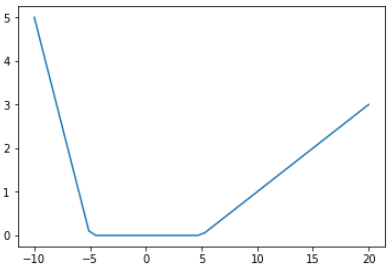
\includegraphics{media/morceaux.png}

    En partant de votre code, vous pouvez produire votre propre courbe en
utilisant \texttt{numpy} et \texttt{matplotlib} comme ceci~:

    \begin{Verbatim}[commandchars=\\\{\}]
{\color{incolor}In [{\color{incolor}6}]:} \PY{c+c1}{\PYZsh{} on importe les bibliothèques}
        \PY{k+kn}{import} \PY{n+nn}{numpy} \PY{k}{as} \PY{n+nn}{np}
        \PY{k+kn}{import} \PY{n+nn}{matplotlib}\PY{n+nn}{.}\PY{n+nn}{pyplot} \PY{k}{as} \PY{n+nn}{plt}
\end{Verbatim}


    \begin{Verbatim}[commandchars=\\\{\}]
{\color{incolor}In [{\color{incolor}7}]:} \PY{c+c1}{\PYZsh{} un échantillon des X entre \PYZhy{}10 et 20}
        \PY{n}{X} \PY{o}{=} \PY{n}{np}\PY{o}{.}\PY{n}{linspace}\PY{p}{(}\PY{o}{\PYZhy{}}\PY{l+m+mi}{10}\PY{p}{,} \PY{l+m+mi}{20}\PY{p}{)}
        
        \PY{c+c1}{\PYZsh{} et les Y correspondants}
        \PY{n}{Y} \PY{o}{=} \PY{n}{np}\PY{o}{.}\PY{n}{vectorize}\PY{p}{(}\PY{n}{morceaux}\PY{p}{)}\PY{p}{(}\PY{n}{X}\PY{p}{)}
\end{Verbatim}


    \begin{Verbatim}[commandchars=\\\{\}]
{\color{incolor}In [{\color{incolor}8}]:} \PY{c+c1}{\PYZsh{} on n\PYZsq{}a plus qu\PYZsq{}à dessiner}
        \PY{n}{plt}\PY{o}{.}\PY{n}{plot}\PY{p}{(}\PY{n}{X}\PY{p}{,} \PY{n}{Y}\PY{p}{)}
        \PY{n}{plt}\PY{o}{.}\PY{n}{show}\PY{p}{(}\PY{p}{)}
\end{Verbatim}


    \begin{center}
    \adjustimage{max size={0.9\linewidth}{0.9\paperheight}}{w2-s6-x4-if-et-def_files/w2-s6-x4-if-et-def_21_0.png}
    \end{center}
    { \hspace*{\fill} \\}
    

    % Add a bibliography block to the postdoc
    
    
    

        
    
    
    

    

    \hypertarget{comptage-dans-les-chaines}{%
\section{Comptage dans les chaines}\label{comptage-dans-les-chaines}}

    \hypertarget{exercice---niveau-basique}{%
\subsection{Exercice - niveau basique}\label{exercice---niveau-basique}}

    Nous remercions Benoit Izac pour cette contribution aux exercices.

    \hypertarget{la-commande-unix-wc1}{%
\subsection{La commande UNIX wc(1)}\label{la-commande-unix-wc1}}

\begin{center}\rule{0.5\linewidth}{\linethickness}\end{center}

Sur les systèmes de type UNIX, la commande
\href{http://pubs.opengroup.org/onlinepubs/9699919799/utilities/wc.html}{wc}
permet de compter le nombre de lignes, de mots et d'octets (ou de
caractères) présents sur l'entrée standard ou contenus dans un fichier.

L'exercice consiste à écrire une fonction nommée \emph{wc} qui prendra
en argument une chaîne de caractères et retournera une liste contenant
trois éléments~:

\begin{enumerate}
\def\labelenumi{\arabic{enumi}.}
\tightlist
\item
  le nombre de lignes (plus précisément le nombre de retours à la
  ligne)~;
\item
  le nombre de mots (un mot étant séparé par des espaces)~;
\item
  le nombre de caractères (on utilisera uniquement le jeu de caractères
  ASCII).
\end{enumerate}

    \begin{Verbatim}[commandchars=\\\{\}]
{\color{incolor}In [{\color{incolor}1}]:} \PY{c+c1}{\PYZsh{} chargement de l\PYZsq{}exercice}
        \PY{k+kn}{from} \PY{n+nn}{corrections}\PY{n+nn}{.}\PY{n+nn}{exo\PYZus{}wc} \PY{k}{import} \PY{n}{exo\PYZus{}wc}
\end{Verbatim}


    \begin{Verbatim}[commandchars=\\\{\}]
{\color{incolor}In [{\color{incolor}2}]:} \PY{c+c1}{\PYZsh{} exemple}
        \PY{n}{exo\PYZus{}wc}\PY{o}{.}\PY{n}{example}\PY{p}{(}\PY{p}{)}
\end{Verbatim}


\begin{Verbatim}[commandchars=\\\{\}]
{\color{outcolor}Out[{\color{outcolor}2}]:} <IPython.core.display.HTML object>
\end{Verbatim}
            
    \textbf{Indice}~: nous avons vu rapidement la boucle \texttt{for},
sachez toutefois qu'on peut tout à fait résoudre l'exercice en utilisant
uniquement la bibliothèque standard.

\textbf{Remarque}~: usuellement, ce genre de fonctions retournerait
plutôt un tuple qu'une liste, mais comme nous ne voyons les tuples que
la semaine prochaine..

    À vous de jouer~:

    \begin{Verbatim}[commandchars=\\\{\}]
{\color{incolor}In [{\color{incolor}3}]:} \PY{c+c1}{\PYZsh{} la fonction à implémenter}
        \PY{k}{def} \PY{n+nf}{wc}\PY{p}{(}\PY{n}{string}\PY{p}{)}\PY{p}{:}
            \PY{c+c1}{\PYZsh{} remplacer pass par votre code}
            \PY{k}{pass}
\end{Verbatim}


    \begin{Verbatim}[commandchars=\\\{\}]
{\color{incolor}In [{\color{incolor} }]:} \PY{c+c1}{\PYZsh{} NOTE}
        \PY{c+c1}{\PYZsh{} auto\PYZhy{}exec\PYZhy{}for\PYZhy{}latex has skipped execution of this cell}
        
        \PY{c+c1}{\PYZsh{} correction}
        \PY{n}{exo\PYZus{}wc}\PY{o}{.}\PY{n}{correction}\PY{p}{(}\PY{n}{wc}\PY{p}{)}
\end{Verbatim}



    % Add a bibliography block to the postdoc
    
    
    

        
    
    
    

    

    \hypertarget{compruxe9hensions-1}{%
\section{Compréhensions (1)}\label{compruxe9hensions-1}}

    \hypertarget{exercice---niveau-basique}{%
\subsection{Exercice - niveau basique}\label{exercice---niveau-basique}}

    \hypertarget{liste-des-valeurs-dune-fonction}{%
\subsubsection{Liste des valeurs d'une
fonction}\label{liste-des-valeurs-dune-fonction}}

    \begin{Verbatim}[commandchars=\\\{\}]
{\color{incolor}In [{\color{incolor}1}]:} \PY{c+c1}{\PYZsh{} Pour charger l\PYZsq{}exercice}
        \PY{k+kn}{from} \PY{n+nn}{corrections}\PY{n+nn}{.}\PY{n+nn}{exo\PYZus{}liste\PYZus{}p} \PY{k}{import} \PY{n}{exo\PYZus{}liste\PYZus{}P}
\end{Verbatim}


    On se donne une fonction polynomiale~:

\(P(x) = 2x^2 - 3x - 2\)

    On vous demande d'écrire une fonction \texttt{liste\_P} qui prend en
argument une liste de nombres réels \(x\) et qui retourne la liste des
valeurs \(P(x)\).

    \begin{Verbatim}[commandchars=\\\{\}]
{\color{incolor}In [{\color{incolor}2}]:} \PY{c+c1}{\PYZsh{} voici un exemple de ce qui est attendu}
        \PY{n}{exo\PYZus{}liste\PYZus{}P}\PY{o}{.}\PY{n}{example}\PY{p}{(}\PY{p}{)}
\end{Verbatim}


\begin{Verbatim}[commandchars=\\\{\}]
{\color{outcolor}Out[{\color{outcolor}2}]:} <IPython.core.display.HTML object>
\end{Verbatim}
            
    Écrivez votre code dans la cellule suivante (\emph{On vous suggère
d'écrire une fonction \texttt{P} qui implémente le polynôme mais ça
n'est pas strictement indispensable, seul le résultat de
\texttt{liste\_P} compte})~:

    \begin{Verbatim}[commandchars=\\\{\}]
{\color{incolor}In [{\color{incolor}3}]:} \PY{k}{def} \PY{n+nf}{P}\PY{p}{(}\PY{n}{x}\PY{p}{)}\PY{p}{:}
            \PY{l+s+s2}{\PYZdq{}}\PY{l+s+s2}{\PYZlt{}votre code\PYZgt{}}\PY{l+s+s2}{\PYZdq{}}
        
        \PY{k}{def} \PY{n+nf}{liste\PYZus{}P}\PY{p}{(}\PY{n}{liste\PYZus{}x}\PY{p}{)}\PY{p}{:}
            \PY{l+s+s2}{\PYZdq{}}\PY{l+s+s2}{votre code}\PY{l+s+s2}{\PYZdq{}}
        
        \PY{c+c1}{\PYZsh{} NOTE:}
        \PY{c+c1}{\PYZsh{} automatic execution has used instead:}
        \PY{c+c1}{\PYZsh{}\PYZsh{}\PYZsh{}\PYZsh{}\PYZsh{}\PYZsh{}\PYZsh{}\PYZsh{}\PYZsh{}\PYZsh{}}
        \PY{n}{liste\PYZus{}P} \PY{o}{=} \PY{n}{exo\PYZus{}liste\PYZus{}P}\PY{o}{.}\PY{n}{solution}
        \PY{c+c1}{\PYZsh{}\PYZsh{}\PYZsh{}\PYZsh{}\PYZsh{}\PYZsh{}\PYZsh{}\PYZsh{}\PYZsh{}\PYZsh{}}
\end{Verbatim}


    Et vous pouvez le vérifier en évaluant cette cellule~:

    \begin{Verbatim}[commandchars=\\\{\}]
{\color{incolor}In [{\color{incolor} }]:} \PY{c+c1}{\PYZsh{} NOTE}
        \PY{c+c1}{\PYZsh{} automatic execution has skipped execution of this cell}
        
        \PY{c+c1}{\PYZsh{} pour vérifier votre code}
        \PY{n}{exo\PYZus{}liste\PYZus{}P}\PY{o}{.}\PY{n}{correction}\PY{p}{(}\PY{n}{liste\PYZus{}P}\PY{p}{)}
\end{Verbatim}


    \begin{center}\rule{0.5\linewidth}{\linethickness}\end{center}

    \hypertarget{ruxe9cruxe9ation}{%
\subsection{Récréation}\label{ruxe9cruxe9ation}}

    Si vous avez correctement implémenté la fonction \texttt{liste\_P} telle
que demandé dans le premier exercice, vous pouvez visualiser le polynôme
\texttt{P} en utilisant \texttt{matplotlib} avec le code suivant~:

    \begin{Verbatim}[commandchars=\\\{\}]
{\color{incolor}In [{\color{incolor}4}]:} \PY{c+c1}{\PYZsh{} on importe les bibliothèques}
        \PY{k+kn}{import} \PY{n+nn}{numpy} \PY{k}{as} \PY{n+nn}{np}
        \PY{k+kn}{import} \PY{n+nn}{matplotlib}\PY{n+nn}{.}\PY{n+nn}{pyplot} \PY{k}{as} \PY{n+nn}{plt}
\end{Verbatim}


    \begin{Verbatim}[commandchars=\\\{\}]
{\color{incolor}In [{\color{incolor}5}]:} \PY{c+c1}{\PYZsh{} un échantillon des X entre \PYZhy{}10 et 10}
        \PY{n}{X} \PY{o}{=} \PY{n}{np}\PY{o}{.}\PY{n}{linspace}\PY{p}{(}\PY{o}{\PYZhy{}}\PY{l+m+mi}{10}\PY{p}{,} \PY{l+m+mi}{10}\PY{p}{)}
        
        \PY{c+c1}{\PYZsh{} et les Y correspondants}
        \PY{n}{Y} \PY{o}{=} \PY{n}{liste\PYZus{}P}\PY{p}{(}\PY{n}{X}\PY{p}{)}
\end{Verbatim}


    \begin{Verbatim}[commandchars=\\\{\}]
{\color{incolor}In [{\color{incolor}6}]:} \PY{c+c1}{\PYZsh{} on n\PYZsq{}a plus qu\PYZsq{}à dessiner}
        \PY{n}{plt}\PY{o}{.}\PY{n}{plot}\PY{p}{(}\PY{n}{X}\PY{p}{,} \PY{n}{Y}\PY{p}{)}
        \PY{n}{plt}\PY{o}{.}\PY{n}{show}\PY{p}{(}\PY{p}{)}
\end{Verbatim}


    \begin{center}
    \adjustimage{max size={0.9\linewidth}{0.9\paperheight}}{w2-s7-x1-liste-p_files/w2-s7-x1-liste-p_17_0.png}
    \end{center}
    { \hspace*{\fill} \\}
    

    % Add a bibliography block to the postdoc
    
    
    

        
    
    
    

    

    \hypertarget{compruxe9hensions-2}{%
\section{Compréhensions (2)}\label{compruxe9hensions-2}}

    \hypertarget{exercice---niveau-intermuxe9diaire}{%
\subsection{Exercice - niveau
intermédiaire}\label{exercice---niveau-intermuxe9diaire}}

    \hypertarget{mise-au-carruxe9}{%
\subsubsection{Mise au carré}\label{mise-au-carruxe9}}

    \begin{Verbatim}[commandchars=\\\{\}]
{\color{incolor}In [{\color{incolor}1}]:} \PY{c+c1}{\PYZsh{} chargement de l\PYZsq{}exercice}
        \PY{k+kn}{from} \PY{n+nn}{corrections}\PY{n+nn}{.}\PY{n+nn}{exo\PYZus{}carre} \PY{k}{import} \PY{n}{exo\PYZus{}carre}
\end{Verbatim}


    On vous demande à présent d'écrire une fonction dans le même esprit que
la fonction polynomiale du notebook précédent. Cette fois, chaque ligne
contient, séparés par des points-virgules, une liste d'entiers, et on
veut obtenir une nouvelle chaîne avec les carrés de ces entiers, séparés
par des deux-points.

À nouveau les lignes peuvent être remplies de manière approximative,
avec des espaces, des tabulations, ou même des points-virgules en trop,
que ce soit au début, à la fin, ou au milieu d'une ligne.

    \begin{Verbatim}[commandchars=\\\{\}]
{\color{incolor}In [{\color{incolor}2}]:} \PY{c+c1}{\PYZsh{} exemples}
        \PY{n}{exo\PYZus{}carre}\PY{o}{.}\PY{n}{example}\PY{p}{(}\PY{p}{)}
\end{Verbatim}


\begin{Verbatim}[commandchars=\\\{\}]
{\color{outcolor}Out[{\color{outcolor}2}]:} <IPython.core.display.HTML object>
\end{Verbatim}
            
    \begin{Verbatim}[commandchars=\\\{\}]
{\color{incolor}In [{\color{incolor}3}]:} \PY{c+c1}{\PYZsh{} écrivez votre code ici}
        \PY{k}{def} \PY{n+nf}{carre}\PY{p}{(}\PY{n}{ligne}\PY{p}{)}\PY{p}{:}
            \PY{l+s+s2}{\PYZdq{}}\PY{l+s+s2}{\PYZlt{}votre\PYZus{}code\PYZgt{}}\PY{l+s+s2}{\PYZdq{}}
\end{Verbatim}


    \begin{Verbatim}[commandchars=\\\{\}]
{\color{incolor}In [{\color{incolor} }]:} \PY{c+c1}{\PYZsh{} NOTE}
        \PY{c+c1}{\PYZsh{} automatic execution has skipped execution of this cell}
        
        \PY{c+c1}{\PYZsh{} pour corriger}
        \PY{n}{exo\PYZus{}carre}\PY{o}{.}\PY{n}{correction}\PY{p}{(}\PY{n}{carre}\PY{p}{)}
\end{Verbatim}



    % Add a bibliography block to the postdoc
    
    
    

    
    \chapter{Renforcement des notions de base, références partagées}

        
    
    
    

    

    \hypertarget{les-fichiers}{%
\section{Les fichiers}\label{les-fichiers}}

    \hypertarget{compluxe9ment---niveau-basique}{%
\subsection{Complément - niveau
basique}\label{compluxe9ment---niveau-basique}}

    Voici quelques utilisations habituelles du type fichier en Python.

    \hypertarget{avec-un-context-manager}{%
\subsubsection{\texorpdfstring{Avec un \emph{context
manager}}{Avec un context manager}}\label{avec-un-context-manager}}

    Nous avons vu dans la vidéo les mécanismes de base sur les fichiers.
Nous avons vu notamment qu'il est important de bien fermer un fichier
après usage. On a vu aussi qu'il est recommandé de \textbf{toujours}
utiliser l'instruction \texttt{with} et de contrôler son encodage. Il
est donc recommandé de faire~:

    \begin{Verbatim}[commandchars=\\\{\},frame=single,framerule=0.3mm,rulecolor=\color{cellframecolor}]
{\color{incolor}In [{\color{incolor}1}]:} \PY{c+c1}{\PYZsh{} avec un `with\PYZsq{} on garantit la fermeture du fichier}
        \PY{k}{with} \PY{n+nb}{open}\PY{p}{(}\PY{l+s+s2}{\PYZdq{}}\PY{l+s+s2}{foo.txt}\PY{l+s+s2}{\PYZdq{}}\PY{p}{,} \PY{l+s+s2}{\PYZdq{}}\PY{l+s+s2}{w}\PY{l+s+s2}{\PYZdq{}}\PY{p}{,} \PY{n}{encoding}\PY{o}{=}\PY{l+s+s1}{\PYZsq{}}\PY{l+s+s1}{utf\PYZhy{}8}\PY{l+s+s1}{\PYZsq{}}\PY{p}{)} \PY{k}{as} \PY{n}{sortie}\PY{p}{:}
            \PY{k}{for} \PY{n}{i} \PY{o+ow}{in} \PY{n+nb}{range}\PY{p}{(}\PY{l+m+mi}{2}\PY{p}{)}\PY{p}{:}
                \PY{n}{sortie}\PY{o}{.}\PY{n}{write}\PY{p}{(}\PY{n}{f}\PY{l+s+s2}{\PYZdq{}}\PY{l+s+si}{\PYZob{}i\PYZcb{}}\PY{l+s+se}{\PYZbs{}n}\PY{l+s+s2}{\PYZdq{}}\PY{p}{)}
\end{Verbatim}


    \hypertarget{les-modes-douverture}{%
\subsubsection{Les modes d'ouverture}\label{les-modes-douverture}}

    Les modes d'ouverture les plus utilisés sont~:

\begin{itemize}
\tightlist
\item
  \texttt{\textquotesingle{}r\textquotesingle{}} (la chaîne contenant
  l'unique caractère \texttt{r}) pour ouvrir un fichier en lecture
  seulement~;
\item
  \texttt{\textquotesingle{}w\textquotesingle{}} en écriture seulement~;
  le contenu précédent du fichier, s'il existait, est perdu~;
\item
  \texttt{\textquotesingle{}a\textquotesingle{}} en écriture seulement~;
  mais pour ajouter du contenu en fin de fichier.
\end{itemize}

    Voici par exemple comment on pourrait ajouter deux lignes de texte dans
le fichier \texttt{foo.txt} qui contient, à ce stade du notebook, deux
entiers~:

    \begin{Verbatim}[commandchars=\\\{\},frame=single,framerule=0.3mm,rulecolor=\color{cellframecolor}]
{\color{incolor}In [{\color{incolor}2}]:} \PY{c+c1}{\PYZsh{} on ouvre le fichier en mode \PYZsq{}a\PYZsq{} comme append (= ajouter)}
        \PY{k}{with} \PY{n+nb}{open}\PY{p}{(}\PY{l+s+s2}{\PYZdq{}}\PY{l+s+s2}{foo.txt}\PY{l+s+s2}{\PYZdq{}}\PY{p}{,} \PY{l+s+s2}{\PYZdq{}}\PY{l+s+s2}{a}\PY{l+s+s2}{\PYZdq{}}\PY{p}{,} \PY{n}{encoding}\PY{o}{=}\PY{l+s+s1}{\PYZsq{}}\PY{l+s+s1}{utf\PYZhy{}8}\PY{l+s+s1}{\PYZsq{}}\PY{p}{)} \PY{k}{as} \PY{n}{sortie}\PY{p}{:}
            \PY{k}{for} \PY{n}{i} \PY{o+ow}{in} \PY{n+nb}{range}\PY{p}{(}\PY{l+m+mi}{100}\PY{p}{,} \PY{l+m+mi}{102}\PY{p}{)}\PY{p}{:}
                \PY{n}{sortie}\PY{o}{.}\PY{n}{write}\PY{p}{(}\PY{n}{f}\PY{l+s+s2}{\PYZdq{}}\PY{l+s+si}{\PYZob{}i\PYZcb{}}\PY{l+s+se}{\PYZbs{}n}\PY{l+s+s2}{\PYZdq{}}\PY{p}{)}
\end{Verbatim}


    \begin{Verbatim}[commandchars=\\\{\},frame=single,framerule=0.3mm,rulecolor=\color{cellframecolor}]
{\color{incolor}In [{\color{incolor}3}]:} \PY{c+c1}{\PYZsh{} maintenant on regarde ce que contient le fichier}
        \PY{c+c1}{\PYZsh{} remarquez que sans \PYZsq{}mode\PYZsq{}, on ouvre en lecture seule}
        \PY{k}{with} \PY{n+nb}{open}\PY{p}{(}\PY{l+s+s2}{\PYZdq{}}\PY{l+s+s2}{foo.txt}\PY{l+s+s2}{\PYZdq{}}\PY{p}{,} \PY{n}{encoding}\PY{o}{=}\PY{l+s+s1}{\PYZsq{}}\PY{l+s+s1}{utf\PYZhy{}8}\PY{l+s+s1}{\PYZsq{}}\PY{p}{)} \PY{k}{as} \PY{n}{entree}\PY{p}{:} 
            \PY{k}{for} \PY{n}{line} \PY{o+ow}{in} \PY{n}{entree}\PY{p}{:}
                \PY{c+c1}{\PYZsh{} line contient déjà un retour à la ligne}
                \PY{n+nb}{print}\PY{p}{(}\PY{n}{line}\PY{p}{,} \PY{n}{end}\PY{o}{=}\PY{l+s+s1}{\PYZsq{}}\PY{l+s+s1}{\PYZsq{}}\PY{p}{)}
\end{Verbatim}


    \begin{Verbatim}[commandchars=\\\{\},frame=single,framerule=0.3mm,rulecolor=\color{cellframecolor}]
0
1
100
101
\end{Verbatim}

    Il existe de nombreuses variantes au mode d'ouverture, pour par
exemple~:

\begin{itemize}
\tightlist
\item
  ouvrir le fichier en lecture \emph{et} en écriture (mode \texttt{+})~;
\item
  ouvrir le fichier en mode binaire (mode \texttt{b}).
\end{itemize}

Ces variantes sont décrites dans
\href{https://docs.python.org/3/library/functions.html\#open}{la section
sur la fonction built-in \texttt{open}} dans la documentation Python.

    \hypertarget{compluxe9ment---niveau-intermuxe9diaire}{%
\subsection{Complément - niveau
intermédiaire}\label{compluxe9ment---niveau-intermuxe9diaire}}

    \hypertarget{un-fichier-est-un-ituxe9rateur}{%
\subsubsection{Un fichier est un
itérateur}\label{un-fichier-est-un-ituxe9rateur}}

    Nous reparlerons des notions d'itérable et d'itérateur dans les semaines
suivantes. Pour l'instant, on peut dire qu'un fichier - qui donc
\textbf{est itérable} puisqu'on peut le lire par une boucle \texttt{for}
- est aussi \textbf{son propre itérateur}. Cela implique que l'on ne
peut le parcourir qu'une fois dans une boucle \texttt{for}. Pour le
reparcourir, il faut le fermer et l'ouvrir de nouveau.

    \begin{Verbatim}[commandchars=\\\{\},frame=single,framerule=0.3mm,rulecolor=\color{cellframecolor}]
{\color{incolor}In [{\color{incolor}4}]:} \PY{c+c1}{\PYZsh{} un fichier est son propre itérateur}
\end{Verbatim}


    \begin{Verbatim}[commandchars=\\\{\},frame=single,framerule=0.3mm,rulecolor=\color{cellframecolor}]
{\color{incolor}In [{\color{incolor}5}]:} \PY{k}{with} \PY{n+nb}{open}\PY{p}{(}\PY{l+s+s2}{\PYZdq{}}\PY{l+s+s2}{foo.txt}\PY{l+s+s2}{\PYZdq{}}\PY{p}{,} \PY{n}{encoding}\PY{o}{=}\PY{l+s+s1}{\PYZsq{}}\PY{l+s+s1}{utf\PYZhy{}8}\PY{l+s+s1}{\PYZsq{}}\PY{p}{)} \PY{k}{as} \PY{n}{entree}\PY{p}{:}
            \PY{n+nb}{print}\PY{p}{(}\PY{n}{entree}\PY{o}{.}\PY{n+nf+fm}{\PYZus{}\PYZus{}iter\PYZus{}\PYZus{}}\PY{p}{(}\PY{p}{)} \PY{o+ow}{is} \PY{n}{entree}\PY{p}{)}
\end{Verbatim}


    \begin{Verbatim}[commandchars=\\\{\},frame=single,framerule=0.3mm,rulecolor=\color{cellframecolor}]
True
\end{Verbatim}

    Par conséquent, écrire deux boucles \texttt{for} imbriquées sur
\textbf{le même objet fichier} ne \textbf{fonctionnerait pas} comme on
pourrait s'y attendre.

    \begin{Verbatim}[commandchars=\\\{\},frame=single,framerule=0.3mm,rulecolor=\color{cellframecolor}]
{\color{incolor}In [{\color{incolor}6}]:} \PY{c+c1}{\PYZsh{} Si l\PYZsq{}on essaie d\PYZsq{}écrire deux boucles imbriquées}
        \PY{c+c1}{\PYZsh{} sur le même objet fichier, le résultat est inattendu}
        \PY{k}{with} \PY{n+nb}{open}\PY{p}{(}\PY{l+s+s2}{\PYZdq{}}\PY{l+s+s2}{foo.txt}\PY{l+s+s2}{\PYZdq{}}\PY{p}{,} \PY{n}{encoding}\PY{o}{=}\PY{l+s+s1}{\PYZsq{}}\PY{l+s+s1}{utf\PYZhy{}8}\PY{l+s+s1}{\PYZsq{}}\PY{p}{)} \PY{k}{as} \PY{n}{entree}\PY{p}{:}
            \PY{k}{for} \PY{n}{l1} \PY{o+ow}{in} \PY{n}{entree}\PY{p}{:}
                \PY{c+c1}{\PYZsh{} on enlève les fins de ligne}
                \PY{n}{l1} \PY{o}{=} \PY{n}{l1}\PY{o}{.}\PY{n}{strip}\PY{p}{(}\PY{p}{)}
                \PY{k}{for} \PY{n}{l2} \PY{o+ow}{in} \PY{n}{entree}\PY{p}{:}
                    \PY{c+c1}{\PYZsh{} on enlève les fins de ligne}
                    \PY{n}{l2} \PY{o}{=} \PY{n}{l2}\PY{o}{.}\PY{n}{strip}\PY{p}{(}\PY{p}{)}
                    \PY{n+nb}{print}\PY{p}{(}\PY{n}{l1}\PY{p}{,} \PY{l+s+s2}{\PYZdq{}}\PY{l+s+s2}{x}\PY{l+s+s2}{\PYZdq{}}\PY{p}{,} \PY{n}{l2}\PY{p}{)}
\end{Verbatim}


    \begin{Verbatim}[commandchars=\\\{\},frame=single,framerule=0.3mm,rulecolor=\color{cellframecolor}]
0 x 1
0 x 100
0 x 101
\end{Verbatim}

    \hypertarget{compluxe9ment---niveau-avancuxe9}{%
\subsection{Complément - niveau
avancé}\label{compluxe9ment---niveau-avancuxe9}}

    \hypertarget{autres-muxe9thodes}{%
\subsubsection{Autres méthodes}\label{autres-muxe9thodes}}

    Vous pouvez également accéder à des fonctions de beaucoup plus bas
niveau, notamment celle fournies directement par le système
d'exploitation~; nous allons en décrire deux parmi les plus utiles.

    \hypertarget{digression---repr}{%
\subparagraph{\texorpdfstring{Digression -
\texttt{repr()}}{Digression - repr()}}\label{digression---repr}}

    Comme nous allons utiliser maintenant des outils d'assez bas niveau pour
lire du texte, pour examiner ce texte nous allons utiliser la fonction
\texttt{repr()}, et voici pourquoi~:

    \begin{Verbatim}[commandchars=\\\{\},frame=single,framerule=0.3mm,rulecolor=\color{cellframecolor}]
{\color{incolor}In [{\color{incolor}7}]:} \PY{c+c1}{\PYZsh{} construisons à la main une chaîne qui contient deux lignes}
        \PY{n}{lines} \PY{o}{=} \PY{l+s+s2}{\PYZdq{}}\PY{l+s+s2}{abc}\PY{l+s+s2}{\PYZdq{}} \PY{o}{+} \PY{l+s+s2}{\PYZdq{}}\PY{l+s+se}{\PYZbs{}n}\PY{l+s+s2}{\PYZdq{}} \PY{o}{+} \PY{l+s+s2}{\PYZdq{}}\PY{l+s+s2}{def}\PY{l+s+s2}{\PYZdq{}}  \PY{o}{+} \PY{l+s+s2}{\PYZdq{}}\PY{l+s+se}{\PYZbs{}n}\PY{l+s+s2}{\PYZdq{}}
\end{Verbatim}


    \begin{Verbatim}[commandchars=\\\{\},frame=single,framerule=0.3mm,rulecolor=\color{cellframecolor}]
{\color{incolor}In [{\color{incolor}8}]:} \PY{c+c1}{\PYZsh{} si on l\PYZsq{}imprime on voit bien les retours à la ligne}
        \PY{c+c1}{\PYZsh{} d\PYZsq{}ailleurs on sait qu\PYZsq{}il n\PYZsq{}est pas utile}
        \PY{c+c1}{\PYZsh{} d\PYZsq{}ajouter un retour à la ligne à la fin}
        \PY{n+nb}{print}\PY{p}{(}\PY{n}{lines}\PY{p}{,} \PY{n}{end}\PY{o}{=}\PY{l+s+s2}{\PYZdq{}}\PY{l+s+s2}{\PYZdq{}}\PY{p}{)}
\end{Verbatim}


    \begin{Verbatim}[commandchars=\\\{\},frame=single,framerule=0.3mm,rulecolor=\color{cellframecolor}]
abc
def
\end{Verbatim}

    \begin{Verbatim}[commandchars=\\\{\},frame=single,framerule=0.3mm,rulecolor=\color{cellframecolor}]
{\color{incolor}In [{\color{incolor}9}]:} \PY{c+c1}{\PYZsh{} vérifions que repr() nous permet de bien}
        \PY{c+c1}{\PYZsh{} voir le contenu de cette chaine}
        \PY{n+nb}{print}\PY{p}{(}\PY{n+nb}{repr}\PY{p}{(}\PY{n}{lines}\PY{p}{)}\PY{p}{)}
\end{Verbatim}


    \begin{Verbatim}[commandchars=\\\{\},frame=single,framerule=0.3mm,rulecolor=\color{cellframecolor}]
'abc\textbackslash{}ndef\textbackslash{}n'
\end{Verbatim}

    \hypertarget{lire-un-contenu---bas-niveau}{%
\subparagraph{Lire un contenu - bas
niveau}\label{lire-un-contenu---bas-niveau}}

    Revenons aux fichiers~; la méthode \texttt{read()} permet de lire dans
le fichier un buffer d'une certaine taille~:

    \begin{Verbatim}[commandchars=\\\{\},frame=single,framerule=0.3mm,rulecolor=\color{cellframecolor}]
{\color{incolor}In [{\color{incolor}10}]:} \PY{c+c1}{\PYZsh{} read() retourne TOUT le contenu}
         \PY{c+c1}{\PYZsh{} ne pas utiliser avec de très gros fichiers bien sûr}
         
         \PY{c+c1}{\PYZsh{} une autre façon de montrer tout le contenu du fichier}
         \PY{k}{with} \PY{n+nb}{open}\PY{p}{(}\PY{l+s+s2}{\PYZdq{}}\PY{l+s+s2}{foo.txt}\PY{l+s+s2}{\PYZdq{}}\PY{p}{,} \PY{n}{encoding}\PY{o}{=}\PY{l+s+s1}{\PYZsq{}}\PY{l+s+s1}{utf\PYZhy{}8}\PY{l+s+s1}{\PYZsq{}}\PY{p}{)} \PY{k}{as} \PY{n}{entree}\PY{p}{:}
             \PY{n}{full\PYZus{}contents} \PY{o}{=} \PY{n}{entree}\PY{o}{.}\PY{n}{read}\PY{p}{(}\PY{p}{)}
             \PY{n+nb}{print}\PY{p}{(}\PY{n}{f}\PY{l+s+s2}{\PYZdq{}}\PY{l+s+s2}{Contenu complet}\PY{l+s+se}{\PYZbs{}n}\PY{l+s+si}{\PYZob{}full\PYZus{}contents\PYZcb{}}\PY{l+s+s2}{\PYZdq{}}\PY{p}{,} \PY{n}{end}\PY{o}{=}\PY{l+s+s2}{\PYZdq{}}\PY{l+s+s2}{\PYZdq{}}\PY{p}{)}
\end{Verbatim}


    \begin{Verbatim}[commandchars=\\\{\},frame=single,framerule=0.3mm,rulecolor=\color{cellframecolor}]
Contenu complet
0
1
100
101
\end{Verbatim}

    \begin{Verbatim}[commandchars=\\\{\},frame=single,framerule=0.3mm,rulecolor=\color{cellframecolor}]
{\color{incolor}In [{\color{incolor}11}]:} \PY{c+c1}{\PYZsh{} lire dans le fichier deux blocs de quatre caractères}
         \PY{k}{with} \PY{n+nb}{open}\PY{p}{(}\PY{l+s+s2}{\PYZdq{}}\PY{l+s+s2}{foo.txt}\PY{l+s+s2}{\PYZdq{}}\PY{p}{,} \PY{n}{encoding}\PY{o}{=}\PY{l+s+s1}{\PYZsq{}}\PY{l+s+s1}{utf\PYZhy{}8}\PY{l+s+s1}{\PYZsq{}}\PY{p}{)} \PY{k}{as} \PY{n}{entree}\PY{p}{:}
             \PY{k}{for} \PY{n}{bloc} \PY{o+ow}{in} \PY{n+nb}{range}\PY{p}{(}\PY{l+m+mi}{2}\PY{p}{)}\PY{p}{:}
                 \PY{n+nb}{print}\PY{p}{(}\PY{n}{f}\PY{l+s+s2}{\PYZdq{}}\PY{l+s+s2}{Bloc }\PY{l+s+si}{\PYZob{}bloc\PYZcb{}}\PY{l+s+s2}{ \PYZgt{}\PYZgt{}}\PY{l+s+s2}{\PYZob{}}\PY{l+s+s2}{repr(entree.read(4))\PYZcb{}\PYZlt{}\PYZlt{}}\PY{l+s+s2}{\PYZdq{}}\PY{p}{)}
\end{Verbatim}


    \begin{Verbatim}[commandchars=\\\{\},frame=single,framerule=0.3mm,rulecolor=\color{cellframecolor}]
Bloc 0 >>'0\textbackslash{}n1\textbackslash{}n'<<
Bloc 1 >>'100\textbackslash{}n'<<
\end{Verbatim}

    On voit donc que chaque bloc contient bien quatre caractères en comptant
les sauts de ligne~:

\begin{longtable}[]{@{}ll@{}}
\toprule
bloc \# & contenu\tabularnewline
\midrule
\endhead
0 & un \texttt{0}, un \emph{newline}, un \texttt{1}, un
\emph{newline}\tabularnewline
1 & un \texttt{1}, deux \texttt{0}, un \emph{newline}\tabularnewline
\bottomrule
\end{longtable}

    \hypertarget{la-muxe9thode-flush}{%
\subparagraph{\texorpdfstring{La méthode
\texttt{flush}}{La méthode flush}}\label{la-muxe9thode-flush}}

    Les entrées-sorties sur fichier sont bien souvent \emph{bufferisées} par
le système d'exploitation. Cela signifie qu'un appel à \texttt{write} ne
provoque pas forcément une écriture immédiate, car pour des raisons de
performance on attend d'avoir suffisamment de matière avant d'écrire sur
le disque.

Il y a des cas où ce comportement peut s'avérer gênant, et où on a
besoin d'écrire immédiatement (et donc de vider le \emph{buffer}), et
c'est le propos de la méthode \texttt{flush}.

    \hypertarget{fichiers-textuels-et-fichiers-binaires}{%
\subsubsection{Fichiers textuels et fichiers
binaires}\label{fichiers-textuels-et-fichiers-binaires}}

    De la même façon que le langage propose les deux types \texttt{str} et
\texttt{bytes}, il est possible d'ouvrir un fichier en mode
\emph{textuel} ou en mode \emph{binaire}.

    Les fichiers que nous avons vus jusqu'ici étaient ouverts en mode
\emph{textuel} (c'est le défaut), et c'est pourquoi nous avons interagi
avec eux avec des objets de type \texttt{str}~:

    \begin{Verbatim}[commandchars=\\\{\},frame=single,framerule=0.3mm,rulecolor=\color{cellframecolor}]
{\color{incolor}In [{\color{incolor}12}]:} \PY{c+c1}{\PYZsh{} un fichier ouvert en mode textuel nous donne des str}
         \PY{k}{with} \PY{n+nb}{open}\PY{p}{(}\PY{l+s+s1}{\PYZsq{}}\PY{l+s+s1}{foo.txt}\PY{l+s+s1}{\PYZsq{}}\PY{p}{,} \PY{n}{encoding}\PY{o}{=}\PY{l+s+s1}{\PYZsq{}}\PY{l+s+s1}{utf\PYZhy{}8}\PY{l+s+s1}{\PYZsq{}}\PY{p}{)} \PY{k}{as} \PY{n+nb}{input}\PY{p}{:}
             \PY{k}{for} \PY{n}{line} \PY{o+ow}{in} \PY{n+nb}{input}\PY{p}{:}
                 \PY{n+nb}{print}\PY{p}{(}\PY{l+s+s2}{\PYZdq{}}\PY{l+s+s2}{on a lu un objet de type}\PY{l+s+s2}{\PYZdq{}}\PY{p}{,} \PY{n+nb}{type}\PY{p}{(}\PY{n}{line}\PY{p}{)}\PY{p}{)}
\end{Verbatim}


    \begin{Verbatim}[commandchars=\\\{\},frame=single,framerule=0.3mm,rulecolor=\color{cellframecolor}]
on a lu un objet de type <class 'str'>
on a lu un objet de type <class 'str'>
on a lu un objet de type <class 'str'>
on a lu un objet de type <class 'str'>
\end{Verbatim}

    Lorsque ce n'est pas le comportement souhaité, on peut~:

\begin{itemize}
\tightlist
\item
  ouvrir le fichier en mode \emph{binaire} - pour cela on ajoute le
  caractère \texttt{b} au mode d'ouverture~;
\item
  et on peut alors interagir avec le fichier avec des objets de type
  \texttt{bytes}
\end{itemize}

    Pour illustrer ce trait, nous allons~: 0. créer un fichier en mode
texte, et y insérer du texte en UTF-8~; 0. relire le fichier en mode
binaire, et retrouver le codage des différents caractères.

    \begin{Verbatim}[commandchars=\\\{\},frame=single,framerule=0.3mm,rulecolor=\color{cellframecolor}]
{\color{incolor}In [{\color{incolor}13}]:} \PY{c+c1}{\PYZsh{} phase 1 : on écrit un fichier avec du texte en UTF\PYZhy{}8}
         \PY{c+c1}{\PYZsh{} on ouvre donc le fichier en mode texte}
         \PY{c+c1}{\PYZsh{} en toute rigueur il faut préciser l\PYZsq{}encodage,}
         \PY{c+c1}{\PYZsh{} si on ne le fait pas il sera déterminé}
         \PY{c+c1}{\PYZsh{} à partir de vos réglages système}
         \PY{k}{with} \PY{n+nb}{open}\PY{p}{(}\PY{l+s+s1}{\PYZsq{}}\PY{l+s+s1}{strbytes}\PY{l+s+s1}{\PYZsq{}}\PY{p}{,} \PY{l+s+s1}{\PYZsq{}}\PY{l+s+s1}{w}\PY{l+s+s1}{\PYZsq{}}\PY{p}{,} \PY{n}{encoding}\PY{o}{=}\PY{l+s+s1}{\PYZsq{}}\PY{l+s+s1}{utf\PYZhy{}8}\PY{l+s+s1}{\PYZsq{}}\PY{p}{)} \PY{k}{as} \PY{n}{output}\PY{p}{:}
             \PY{n}{output}\PY{o}{.}\PY{n}{write}\PY{p}{(}\PY{l+s+s2}{\PYZdq{}}\PY{l+s+s2}{déjà l}\PY{l+s+s2}{\PYZsq{}}\PY{l+s+s2}{été}\PY{l+s+se}{\PYZbs{}n}\PY{l+s+s2}{\PYZdq{}}\PY{p}{)}
\end{Verbatim}


    \begin{Verbatim}[commandchars=\\\{\},frame=single,framerule=0.3mm,rulecolor=\color{cellframecolor}]
{\color{incolor}In [{\color{incolor}14}]:} \PY{c+c1}{\PYZsh{} phase 2: on ouvre le fichier en mode binaire}
         \PY{k}{with} \PY{n+nb}{open}\PY{p}{(}\PY{l+s+s1}{\PYZsq{}}\PY{l+s+s1}{strbytes}\PY{l+s+s1}{\PYZsq{}}\PY{p}{,} \PY{l+s+s1}{\PYZsq{}}\PY{l+s+s1}{rb}\PY{l+s+s1}{\PYZsq{}}\PY{p}{)} \PY{k}{as} \PY{n}{rawinput}\PY{p}{:}
             \PY{c+c1}{\PYZsh{} on lit tout le contenu}
             \PY{n}{octets} \PY{o}{=} \PY{n}{rawinput}\PY{o}{.}\PY{n}{read}\PY{p}{(}\PY{p}{)}
             \PY{c+c1}{\PYZsh{} qui est de type bytes}
             \PY{n+nb}{print}\PY{p}{(}\PY{l+s+s2}{\PYZdq{}}\PY{l+s+s2}{on a lu un objet de type}\PY{l+s+s2}{\PYZdq{}}\PY{p}{,} \PY{n+nb}{type}\PY{p}{(}\PY{n}{octets}\PY{p}{)}\PY{p}{)}
             \PY{c+c1}{\PYZsh{} si on regarde chaque octet un par un}
             \PY{k}{for} \PY{n}{i}\PY{p}{,} \PY{n}{octet} \PY{o+ow}{in} \PY{n+nb}{enumerate}\PY{p}{(}\PY{n}{octets}\PY{p}{)}\PY{p}{:}
                 \PY{n+nb}{print}\PY{p}{(}\PY{n}{f}\PY{l+s+s2}{\PYZdq{}}\PY{l+s+si}{\PYZob{}i\PYZcb{}}\PY{l+s+s2}{ → }\PY{l+s+s2}{\PYZob{}}\PY{l+s+s2}{repr(chr(octet))\PYZcb{} [}\PY{l+s+s2}{\PYZob{}}\PY{l+s+s2}{hex(octet)\PYZcb{}]}\PY{l+s+s2}{\PYZdq{}}\PY{p}{)}
\end{Verbatim}


    \begin{Verbatim}[commandchars=\\\{\},frame=single,framerule=0.3mm,rulecolor=\color{cellframecolor}]
on a lu un objet de type <class 'bytes'>
0 → 'd' [0x64]
1 → 'Ã' [0xc3]
2 → '©' [0xa9]
3 → 'j' [0x6a]
4 → 'Ã' [0xc3]
5 → '\textbackslash{}xa0' [0xa0]
6 → ' ' [0x20]
7 → 'l' [0x6c]
8 → "'" [0x27]
9 → 'Ã' [0xc3]
10 → '©' [0xa9]
11 → 't' [0x74]
12 → 'Ã' [0xc3]
13 → '©' [0xa9]
14 → '\textbackslash{}n' [0xa]
\end{Verbatim}

    Vous retrouvez ainsi le fait que l'unique caractère Unicode \texttt{é} a
été encodé par UTF-8 sous la forme de deux octets de code hexadécimal
\texttt{0xc3} et \texttt{0xa9}.

    Vous pouvez également consulter ce site qui visualise l'encodage UTF-8,
avec notre séquence d'entrée~:

https://mothereff.in/utf-8\#d\%C3\%A9j\%C3\%A0\%20l\%27\%C3\%A9t\%C3\%A9\%0A

    \begin{Verbatim}[commandchars=\\\{\},frame=single,framerule=0.3mm,rulecolor=\color{cellframecolor}]
{\color{incolor}In [{\color{incolor}15}]:} \PY{c+c1}{\PYZsh{} on peut comparer le nombre d\PYZsq{}octets et le nombre de caractères}
         \PY{k}{with} \PY{n+nb}{open}\PY{p}{(}\PY{l+s+s1}{\PYZsq{}}\PY{l+s+s1}{strbytes}\PY{l+s+s1}{\PYZsq{}}\PY{p}{,} \PY{n}{encoding}\PY{o}{=}\PY{l+s+s1}{\PYZsq{}}\PY{l+s+s1}{utf\PYZhy{}8}\PY{l+s+s1}{\PYZsq{}}\PY{p}{)} \PY{k}{as} \PY{n}{textfile}\PY{p}{:}
             \PY{n+nb}{print}\PY{p}{(}\PY{n}{f}\PY{l+s+s2}{\PYZdq{}}\PY{l+s+s2}{en mode texte, }\PY{l+s+s2}{\PYZob{}}\PY{l+s+s2}{len(textfile.read())\PYZcb{} caractères}\PY{l+s+s2}{\PYZdq{}}\PY{p}{)}
         \PY{k}{with} \PY{n+nb}{open}\PY{p}{(}\PY{l+s+s1}{\PYZsq{}}\PY{l+s+s1}{strbytes}\PY{l+s+s1}{\PYZsq{}}\PY{p}{,} \PY{l+s+s1}{\PYZsq{}}\PY{l+s+s1}{rb}\PY{l+s+s1}{\PYZsq{}}\PY{p}{)} \PY{k}{as} \PY{n}{binfile}\PY{p}{:}
             \PY{n+nb}{print}\PY{p}{(}\PY{n}{f}\PY{l+s+s2}{\PYZdq{}}\PY{l+s+s2}{en mode binaire, }\PY{l+s+s2}{\PYZob{}}\PY{l+s+s2}{len(binfile.read())\PYZcb{} octets}\PY{l+s+s2}{\PYZdq{}}\PY{p}{)}
\end{Verbatim}


    \begin{Verbatim}[commandchars=\\\{\},frame=single,framerule=0.3mm,rulecolor=\color{cellframecolor}]
en mode texte, 11 caractères
en mode binaire, 15 octets
\end{Verbatim}

    Ce qui correspond au fait que nos quatre caractères non-ASCII (3 x
\texttt{é} et 1 x \texttt{à}) sont tous encodés par UTF-8 comme deux
octets, comme vous pouvez vous en assurer
\href{https://mothereff.in/utf-8\#\%C3\%A9}{ici pour \texttt{é}} et
\href{https://mothereff.in/utf-8\#\%C3\%A0}{là pour \texttt{à}}.

    \hypertarget{pour-en-savoir-plus}{%
\subsubsection{Pour en savoir plus}\label{pour-en-savoir-plus}}

    Pour une description exhaustive vous pouvez vous reporter~:

\begin{itemize}
\tightlist
\item
  au
  \href{https://docs.python.org/3/glossary.html\#term-file-object}{glossaire
  sur la notion de \texttt{object\ file}},
\item
  et aussi et surtout
  \href{https://docs.python.org/3/library/io.html\#module-io}{au module
  \texttt{io}} qui décrit plus en détail les fonctionnalités
  disponibles.
\end{itemize}


    % Add a bibliography block to the postdoc
    
    
    
    
        
    
    
    

    

    \hypertarget{fichiers-et-utilitaires}{%
\section{Fichiers et utilitaires}\label{fichiers-et-utilitaires}}

    \hypertarget{compluxe9ment---niveau-basique}{%
\subsection{Complément - niveau
basique}\label{compluxe9ment---niveau-basique}}

    Outre les objets fichiers créés avec la fonction \texttt{open}, comme on
l'a vu dans la vidéo, et qui servent à lire et écrire à un endroit
précis, une application a besoin d'un minimum d'utilitaires pour
\textbf{parcourir l'arborescence de répertoires et fichiers}, c'est
notre propos dans ce complément.

    \hypertarget{le-module-os.path-obsoluxe8te}{%
\subsubsection{\texorpdfstring{Le module \texttt{os.path}
(obsolète)}{Le module os.path (obsolète)}}\label{le-module-os.path-obsoluxe8te}}

    Avant la version python-3.4, la librairie standard offrait une
conjonction d'outils pour ce type de fonctionnalités:

\begin{itemize}
\tightlist
\item
  le module \texttt{os.path}, pour faire des calculs sur les les chemins
  et noms de fichiers
  \href{https://docs.python.org/3/library/os.html}{doc},
\item
  le module \texttt{os} pour certaines fonctions complémentaires comme
  renommer ou détruire un fichier
  \href{https://docs.python.org/3/library/os.path.html}{doc},
\item
  et enfin le module \texttt{glob} pour la recherche de fichiers, par
  exemple pour trouver tous les fichiers en \texttt{*.txt}
  \href{https://docs.python.org/3/library/glob.html}{doc}.
\end{itemize}

    Cet ensemble un peu disparate a été remplacé par une \textbf{librairie
unique \texttt{pathlib}}, qui fournit toutes ces fonctionnalités sous un
interface unique et moderne, que nous \textbf{recommandons} évidemment
d'utiliser pour \textbf{du nouveau code}.

Avant d'aborder \texttt{pathlib}, voici un très bref aperçu de ces trois
anciens modules, pour le cas - assez probable - où vous les
rencontreriez dans du code existant; tous les noms qui suivent
correspondent à des \textbf{fonctions} - par opposition à
\texttt{pathlib} qui, comme nous allons le voir, offre une interface
orientée objet:

    \begin{itemize}
\tightlist
\item
  \texttt{os.path.join} ajoute `/' ou '' entre deux morceaux de chemin,
  selon l'OS
\item
  \texttt{os.path.basename} trouve le nom de fichier dans un chemin
\item
  \texttt{os.path.dirname} trouve le nom du directory dans un chemin
\item
  \texttt{os.path.abspath} calcule un chemin absolu, c'est-à-dire à
  partir de la racine du filesystem
\end{itemize}

    \begin{itemize}
\tightlist
\item
  \texttt{os.path.exists} pour savoir si un chemin existe ou pas
  (fichier ou répertoire)
\item
  \texttt{os.path.isfile} (et \texttt{isdir}) pour savoir si un chemin
  est un fichier (et un répertoire)
\item
  \texttt{os.path.getsize} pour obtenir la taille du fichier
\item
  \texttt{os.path.getatime} et aussi \texttt{getmtime} et
  \texttt{getctime} pour obtenir les dates de création/modification d'un
  fichier
\end{itemize}

    \begin{itemize}
\tightlist
\item
  \texttt{os.remove} (ou son ancien nom \texttt{os.unlink}), qui permet
  de supprimer un fichier
\item
  \texttt{os.rmdir} pour supprimer un répertoire (mais qui doit être
  vide)
\item
  \texttt{os.removedirs} pour supprimer tout un répertoire avec son
  contenu, récursivement si nécessaire
\item
  \texttt{os.rename} pour renommer un fichier
\end{itemize}

    \begin{itemize}
\tightlist
\item
  \texttt{glob.glob} comme dans par exemple \texttt{glob.glob("*.txt")}
\end{itemize}

    \hypertarget{le-module-pathlib}{%
\subsubsection{\texorpdfstring{Le module
\texttt{pathlib}}{Le module pathlib}}\label{le-module-pathlib}}

    C'est la méthode recommandée aujourd'hui pour travailler sur les
fichiers et répertoires.

    \hypertarget{orientuxe9-objet}{%
\subparagraph{Orienté Objet}\label{orientuxe9-objet}}

    Comme on l'a mentionné \texttt{pathlib} offre une interface orientée
objet; mais qu'est-ce que ça veut dire au juste ?

Ceci nous donne un prétexte pour une première application pratique des
notions de module (que nous avons introduits en fin de semaine 2) et de
classe (que nous allons voir en fin de semaine).

    De même que le langage nous propose les types \emph{builtin}
\texttt{int} et \texttt{str}, le module \texttt{pathlib} nous expose
\textbf{un type} (on dira plutôt \textbf{une classe}) qui s'appelle
\texttt{Path}, que nous allons importer comme ceci:

    \begin{Verbatim}[commandchars=\\\{\}]
{\color{incolor}In [{\color{incolor}1}]:} \PY{k+kn}{from} \PY{n+nn}{pathlib} \PY{k}{import} \PY{n}{Path}
\end{Verbatim}


    Nous allons faire tourner un petit scénario qui va créer un fichier:

    \begin{Verbatim}[commandchars=\\\{\}]
{\color{incolor}In [{\color{incolor}2}]:} \PY{c+c1}{\PYZsh{} le nom de notre fichier jouet }
        \PY{n}{nom} \PY{o}{=} \PY{l+s+s1}{\PYZsq{}}\PY{l+s+s1}{fichier\PYZhy{}temoin}\PY{l+s+s1}{\PYZsq{}}
\end{Verbatim}


    Pour commencer, nous allons vérifier si le fichier en question existe.

Pour ça nous créons un \textbf{objet} qui est une \textbf{instance} de
la classe \texttt{Path}, comme ceci:

    \begin{Verbatim}[commandchars=\\\{\}]
{\color{incolor}In [{\color{incolor}3}]:} \PY{c+c1}{\PYZsh{} on crée un objet de la classe Path, associé au nom de fichier}
        \PY{n}{path} \PY{o}{=} \PY{n}{Path}\PY{p}{(}\PY{n}{nom}\PY{p}{)}
\end{Verbatim}


    Vous remarquez que c'est cohérent avec par exemple:

    \begin{Verbatim}[commandchars=\\\{\}]
{\color{incolor}In [{\color{incolor}4}]:} \PY{c+c1}{\PYZsh{} transformer un float en int}
        \PY{n}{i} \PY{o}{=} \PY{n+nb}{int}\PY{p}{(}\PY{l+m+mf}{3.5}\PY{p}{)}
\end{Verbatim}


    en ce sens que le type (\texttt{int} ou \texttt{Path}) se comporte comme
une usine pour créer des objets du type en question.

    Quoi qu'il en soit, cet objet \texttt{path} offre un certain nombre de
méthodes; pour les voir puisque nous sommes dans un notebook, je vous
invite dans la cellule suivante à utiliser l'aide en ligne en appuyant
sur la touche `Tabulation' après avoir ajouté un \texttt{.} comme si
vous alliez envoyer une méthode à cet objet

\begin{verbatim}
path.[taper la touche TAB]
\end{verbatim}

et le notebook vous montrera la liste des méthodes disponibles.

    \begin{Verbatim}[commandchars=\\\{\}]
{\color{incolor}In [{\color{incolor}5}]:} \PY{c+c1}{\PYZsh{} ajouter un . et utilisez la touche \PYZlt{}Tabulation\PYZgt{}}
        \PY{n}{path}
\end{Verbatim}


\begin{Verbatim}[commandchars=\\\{\}]
{\color{outcolor}Out[{\color{outcolor}5}]:} PosixPath('fichier-temoin')
\end{Verbatim}
            
    Ainsi par exemple on peut savoir si le fichier existe avec la méthode
\texttt{exists()}

    \begin{Verbatim}[commandchars=\\\{\}]
{\color{incolor}In [{\color{incolor}6}]:} \PY{c+c1}{\PYZsh{} au départ le fichier n\PYZsq{}existe pas}
        \PY{n}{path}\PY{o}{.}\PY{n}{exists}\PY{p}{(}\PY{p}{)}
\end{Verbatim}


\begin{Verbatim}[commandchars=\\\{\}]
{\color{outcolor}Out[{\color{outcolor}6}]:} False
\end{Verbatim}
            
    \begin{Verbatim}[commandchars=\\\{\}]
{\color{incolor}In [{\color{incolor}7}]:} \PY{c+c1}{\PYZsh{} si j\PYZsq{}écris dedans je le crée}
        \PY{k}{with} \PY{n+nb}{open}\PY{p}{(}\PY{n}{nom}\PY{p}{,} \PY{l+s+s1}{\PYZsq{}}\PY{l+s+s1}{w}\PY{l+s+s1}{\PYZsq{}}\PY{p}{,} \PY{n}{encoding}\PY{o}{=}\PY{l+s+s1}{\PYZsq{}}\PY{l+s+s1}{utf\PYZhy{}8}\PY{l+s+s1}{\PYZsq{}}\PY{p}{)} \PY{k}{as} \PY{n}{output}\PY{p}{:}
            \PY{n}{output}\PY{o}{.}\PY{n}{write}\PY{p}{(}\PY{l+s+s1}{\PYZsq{}}\PY{l+s+s1}{0123456789}\PY{l+s+se}{\PYZbs{}n}\PY{l+s+s1}{\PYZsq{}}\PY{p}{)}
\end{Verbatim}


    \begin{Verbatim}[commandchars=\\\{\}]
{\color{incolor}In [{\color{incolor}8}]:} \PY{c+c1}{\PYZsh{} et maintenant il existe}
        \PY{n}{path}\PY{o}{.}\PY{n}{exists}\PY{p}{(}\PY{p}{)}
\end{Verbatim}


\begin{Verbatim}[commandchars=\\\{\}]
{\color{outcolor}Out[{\color{outcolor}8}]:} True
\end{Verbatim}
            
    \hypertarget{muxe9tadonnuxe9es}{%
\subparagraph{Métadonnées}\label{muxe9tadonnuxe9es}}

    Voici quelques exemples qui montrent comment accéder aux métadonnées de
ce fichier:

    \begin{Verbatim}[commandchars=\\\{\}]
{\color{incolor}In [{\color{incolor}9}]:} \PY{c+c1}{\PYZsh{} cette méthode retourne (en un seul appel système) les métadonnées agrégées}
        \PY{n}{path}\PY{o}{.}\PY{n}{stat}\PY{p}{(}\PY{p}{)}
\end{Verbatim}


\begin{Verbatim}[commandchars=\\\{\}]
{\color{outcolor}Out[{\color{outcolor}9}]:} os.stat\_result(st\_mode=33188, st\_ino=17121245, st\_dev=16777220, st\_nlink=1, st\_uid=501, st\_gid=20, st\_size=11, st\_atime=1540558080, st\_mtime=1540558080, st\_ctime=1540558080)
\end{Verbatim}
            
    Pour ceux que ça intéresse, l'objet retourné par cette méthode
\texttt{stat} est un \texttt{namedtuple}, que l'on va voir très bientôt.

On accède aux différentes informations comme ceci:

    \begin{Verbatim}[commandchars=\\\{\}]
{\color{incolor}In [{\color{incolor}10}]:} \PY{c+c1}{\PYZsh{} la taille du fichier en octets est de 11 }
         \PY{c+c1}{\PYZsh{} car il faut compter un caractère \PYZdq{}newline\PYZdq{} en fin de ligne }
         \PY{n}{path}\PY{o}{.}\PY{n}{stat}\PY{p}{(}\PY{p}{)}\PY{o}{.}\PY{n}{st\PYZus{}size}
\end{Verbatim}


\begin{Verbatim}[commandchars=\\\{\}]
{\color{outcolor}Out[{\color{outcolor}10}]:} 11
\end{Verbatim}
            
    \begin{Verbatim}[commandchars=\\\{\}]
{\color{incolor}In [{\color{incolor}11}]:} \PY{c+c1}{\PYZsh{} la date de dernière modification, sous forme d\PYZsq{}un nombre}
         \PY{c+c1}{\PYZsh{} c\PYZsq{}est le nombre de secondes depuis le 1er Janvier 1970}
         \PY{n}{mtime} \PY{o}{=} \PY{n}{path}\PY{o}{.}\PY{n}{stat}\PY{p}{(}\PY{p}{)}\PY{o}{.}\PY{n}{st\PYZus{}mtime}
         \PY{n}{mtime}
\end{Verbatim}


\begin{Verbatim}[commandchars=\\\{\}]
{\color{outcolor}Out[{\color{outcolor}11}]:} 1540558080.0
\end{Verbatim}
            
    \begin{Verbatim}[commandchars=\\\{\}]
{\color{incolor}In [{\color{incolor}12}]:} \PY{c+c1}{\PYZsh{} que je peux rendre lisible comme ceci}
         \PY{c+c1}{\PYZsh{} en anticipant sur le module datetime}
         \PY{k+kn}{from} \PY{n+nn}{datetime} \PY{k}{import} \PY{n}{datetime}
         \PY{n}{mtime\PYZus{}datetime} \PY{o}{=} \PY{n}{datetime}\PY{o}{.}\PY{n}{fromtimestamp}\PY{p}{(}\PY{n}{mtime}\PY{p}{)}
         \PY{n}{mtime\PYZus{}datetime}
\end{Verbatim}


\begin{Verbatim}[commandchars=\\\{\}]
{\color{outcolor}Out[{\color{outcolor}12}]:} datetime.datetime(2018, 10, 26, 14, 48)
\end{Verbatim}
            
    \begin{Verbatim}[commandchars=\\\{\}]
{\color{incolor}In [{\color{incolor}13}]:} \PY{c+c1}{\PYZsh{} ou encore, si je formatte pour n\PYZsq{}obtenir que}
         \PY{c+c1}{\PYZsh{} l\PYZsq{}heure et la minute}
         \PY{n}{f}\PY{l+s+s2}{\PYZdq{}}\PY{l+s+s2}{\PYZob{}}\PY{l+s+s2}{mtime\PYZus{}datetime:}\PY{l+s+s2}{\PYZpc{}}\PY{l+s+s2}{H:}\PY{l+s+s2}{\PYZpc{}}\PY{l+s+s2}{M\PYZcb{}}\PY{l+s+s2}{\PYZdq{}}
\end{Verbatim}


\begin{Verbatim}[commandchars=\\\{\}]
{\color{outcolor}Out[{\color{outcolor}13}]:} '14:48'
\end{Verbatim}
            
    \hypertarget{duxe9truire-un-fichier}{%
\subparagraph{Détruire un fichier}\label{duxe9truire-un-fichier}}

    \begin{Verbatim}[commandchars=\\\{\}]
{\color{incolor}In [{\color{incolor}14}]:} \PY{c+c1}{\PYZsh{} je peux maintenant détruire le fichier}
         \PY{n}{path}\PY{o}{.}\PY{n}{unlink}\PY{p}{(}\PY{p}{)}
\end{Verbatim}


    \begin{Verbatim}[commandchars=\\\{\}]
{\color{incolor}In [{\color{incolor}15}]:} \PY{c+c1}{\PYZsh{} ou encore mieux, si je veux détruire }
         \PY{c+c1}{\PYZsh{} seulement dans le cas où il existe je peux aussi faire}
         \PY{k}{try}\PY{p}{:} 
             \PY{n}{path}\PY{o}{.}\PY{n}{unlink}\PY{p}{(}\PY{p}{)}
         \PY{k}{except} \PY{n+ne}{FileNotFoundError}\PY{p}{:}
             \PY{n+nb}{print}\PY{p}{(}\PY{l+s+s2}{\PYZdq{}}\PY{l+s+s2}{no need to remove}\PY{l+s+s2}{\PYZdq{}}\PY{p}{)}
\end{Verbatim}


    \begin{Verbatim}[commandchars=\\\{\}]
no need to remove

    \end{Verbatim}

    \begin{Verbatim}[commandchars=\\\{\}]
{\color{incolor}In [{\color{incolor}16}]:} \PY{c+c1}{\PYZsh{} et maintenant il n\PYZsq{}existe plus}
         \PY{n}{path}\PY{o}{.}\PY{n}{exists}\PY{p}{(}\PY{p}{)}
\end{Verbatim}


\begin{Verbatim}[commandchars=\\\{\}]
{\color{outcolor}Out[{\color{outcolor}16}]:} False
\end{Verbatim}
            
    \begin{Verbatim}[commandchars=\\\{\}]
{\color{incolor}In [{\color{incolor}17}]:} \PY{c+c1}{\PYZsh{} je peux aussi retrouver le nom du fichier comme ceci}
         \PY{c+c1}{\PYZsh{} attention ce n\PYZsq{}est pas une méthode mais un attribut }
         \PY{c+c1}{\PYZsh{} c\PYZsq{}est pourquoi il n\PYZsq{}y a pas de parenthèses}
         \PY{n}{path}\PY{o}{.}\PY{n}{name}
\end{Verbatim}


\begin{Verbatim}[commandchars=\\\{\}]
{\color{outcolor}Out[{\color{outcolor}17}]:} 'fichier-temoin'
\end{Verbatim}
            
    \hypertarget{recherche-de-fichiers}{%
\subparagraph{Recherche de fichiers}\label{recherche-de-fichiers}}

    Maintenant je voudrais connaître la liste des fichiers de nom
\texttt{*.json} dans le directory \texttt{data}.

La méthode la plus naturelle consiste à créer une instance de
\texttt{Path} associée au directory lui-même:

    \begin{Verbatim}[commandchars=\\\{\}]
{\color{incolor}In [{\color{incolor}18}]:} \PY{n}{dirpath} \PY{o}{=} \PY{n}{Path}\PY{p}{(}\PY{l+s+s1}{\PYZsq{}}\PY{l+s+s1}{./data/}\PY{l+s+s1}{\PYZsq{}}\PY{p}{)}
\end{Verbatim}


    Sur cet objet la méthode \texttt{glob} nous retourne un itérable qui
contient ce qu'on veut:

    \begin{Verbatim}[commandchars=\\\{\}]
{\color{incolor}In [{\color{incolor}19}]:} \PY{c+c1}{\PYZsh{} tous les fichiers *.json dans le répertoire data/}
         \PY{k}{for} \PY{n}{json} \PY{o+ow}{in} \PY{n}{dirpath}\PY{o}{.}\PY{n}{glob}\PY{p}{(}\PY{l+s+s2}{\PYZdq{}}\PY{l+s+s2}{*.json}\PY{l+s+s2}{\PYZdq{}}\PY{p}{)}\PY{p}{:}
             \PY{n+nb}{print}\PY{p}{(}\PY{n}{json}\PY{p}{)}
\end{Verbatim}


    \begin{Verbatim}[commandchars=\\\{\}]
data/cities\_europe.json
data/cities\_foo.json
data/cities\_france.json
data/cities\_idf.json
data/cities\_nice.json
data/cities\_world.json
data/marine-abb.json
data/marine-e1-abb.json
data/marine-e1-ext.json
data/marine-e2-abb.json
data/marine-e2-ext.json
data/marine-ext.json
data/meteo\_europe.json
data/meteo\_france.json
data/meteo\_world.json

    \end{Verbatim}

    \hypertarget{documentation-compluxe8te}{%
\subparagraph{Documentation complète}\label{documentation-compluxe8te}}

    Voyez \href{https://docs.python.org/3/library/pathlib.html}{la
documentation complète ici}

    \hypertarget{compluxe9ment---niveau-avancuxe9}{%
\subsection{Complément - niveau
avancé}\label{compluxe9ment---niveau-avancuxe9}}

    Pour ceux qui sont déjà familiers avec les classes, j'en profite pour
vous faire remarquer le type de notre objet path

    \begin{Verbatim}[commandchars=\\\{\}]
{\color{incolor}In [{\color{incolor}20}]:} \PY{n+nb}{type}\PY{p}{(}\PY{n}{path}\PY{p}{)}
\end{Verbatim}


\begin{Verbatim}[commandchars=\\\{\}]
{\color{outcolor}Out[{\color{outcolor}20}]:} pathlib.PosixPath
\end{Verbatim}
            
    qui n'est pas \texttt{Path}, mais en fait une sous-classe de
\texttt{Path} qui est - sur la plateforme du MOOC au moins, qui
fonctionne sous linux - un objet de type \texttt{PosixPath}, qui est une
sous-classe de \texttt{Path}, comme vous pouvez le voir:

    \begin{Verbatim}[commandchars=\\\{\}]
{\color{incolor}In [{\color{incolor}21}]:} \PY{k+kn}{from} \PY{n+nn}{pathlib} \PY{k}{import} \PY{n}{PosixPath}
         \PY{n+nb}{issubclass}\PY{p}{(}\PY{n}{PosixPath}\PY{p}{,} \PY{n}{Path}\PY{p}{)}
\end{Verbatim}


\begin{Verbatim}[commandchars=\\\{\}]
{\color{outcolor}Out[{\color{outcolor}21}]:} True
\end{Verbatim}
            
    Ce qui fait que mécaniquement, path est bien une instance de
\texttt{Path}

    \begin{Verbatim}[commandchars=\\\{\}]
{\color{incolor}In [{\color{incolor}22}]:} \PY{n+nb}{isinstance}\PY{p}{(}\PY{n}{path}\PY{p}{,} \PY{n}{Path}\PY{p}{)}
\end{Verbatim}


\begin{Verbatim}[commandchars=\\\{\}]
{\color{outcolor}Out[{\color{outcolor}22}]:} True
\end{Verbatim}
            
    ce qui est heureux puisqu'on avait utilisé \texttt{Path()} pour
construire l'objet \texttt{path} au départ :)


    % Add a bibliography block to the postdoc
    
    
    

        
    
    
    

    

    \hypertarget{formats-de-fichiers-json-et-autres}{%
\section{Formats de fichiers~: JSON et
autres}\label{formats-de-fichiers-json-et-autres}}

    \hypertarget{compluxe9ments---niveau-basique}{%
\subsection{Compléments - niveau
basique}\label{compluxe9ments---niveau-basique}}

    Voici quelques mots sur des outils Python fournis dans la bibliothèque
standard, et qui permettent de lire ou écrire des données dans des
fichiers.

    \hypertarget{le-probluxe8me}{%
\subsubsection{Le problème}\label{le-probluxe8me}}

    Les données dans un programme Python sont stockées en mémoire (la RAM),
sous une forme propice aux calculs. Par exemple un petit entier est
fréquemment stocké en binaire dans un mot de 64 bits, qui est prêt à
être soumis au processeur pour faire une opération arithmétique.

    Ce format ne se prête pas forcément toujours à être transposé tel quel
lorsqu'on doit écrire des données sur un support plus pérenne, comme un
disque dur, ou encore sur un réseau pour transmission distante - ces
deux supports étant à ce point de vue très voisins.

Ainsi par exemple il pourra être plus commode d'écrire notre entier sur
disque, ou de le transmettre à un programme distant, sous une forme
décimale qui sera plus lisible, sachant que par ailleurs toutes les
machines ne codent pas un entier de la même façon.

    Il convient donc de faire de la traduction dans les deux sens entre
représentations d'une part en mémoire, et d'autre part sur disque ou sur
réseau (à nouveau, on utilise en général les mêmes formats pour ces deux
usages).

    \hypertarget{le-format-json}{%
\subsubsection{Le format JSON}\label{le-format-json}}

    Le format sans aucun doute le plus populaire à l'heure actuelle est
\href{http://fr.wikipedia.org/wiki/JavaScript_Object_Notation}{le format
JSON} pour \emph{JavaScript Object Notation}.

Sans trop nous attarder nous dirons que JSON est un encodage - en
anglais
\href{http://en.wikipedia.org/wiki/Marshalling_\%28computer_science\%29}{marshalling}
- qui se prête bien à la plupart des types de base que l'on trouve dans
les langages modernes comme Python, Ruby ou JavaScript.

La bibliothèque standard de Python contient
\href{https://docs.python.org/3/library/json.html}{le module json} que
nous illustrons très rapidement ici~:

    \begin{Verbatim}[commandchars=\\\{\},frame=single,framerule=0.3mm,rulecolor=\color{cellframecolor}]
{\color{incolor}In [{\color{incolor}1}]:} \PY{k+kn}{import} \PY{n+nn}{json}
        
        \PY{c+c1}{\PYZsh{} En partant d\PYZsq{}une donnée construite à partir de types de base}
        \PY{n}{data} \PY{o}{=} \PY{p}{[}
            \PY{c+c1}{\PYZsh{} des types qui ne posent pas de problème}
            \PY{p}{[}\PY{l+m+mi}{1}\PY{p}{,} \PY{l+m+mi}{2}\PY{p}{,} \PY{l+s+s1}{\PYZsq{}}\PY{l+s+s1}{a}\PY{l+s+s1}{\PYZsq{}}\PY{p}{,} \PY{p}{[}\PY{l+m+mf}{3.23}\PY{p}{,} \PY{l+m+mf}{4.32}\PY{p}{]}\PY{p}{,} \PY{p}{\PYZob{}}\PY{l+s+s1}{\PYZsq{}}\PY{l+s+s1}{eric}\PY{l+s+s1}{\PYZsq{}}\PY{p}{:} \PY{l+m+mi}{32}\PY{p}{,} \PY{l+s+s1}{\PYZsq{}}\PY{l+s+s1}{jean}\PY{l+s+s1}{\PYZsq{}}\PY{p}{:} \PY{l+m+mi}{43}\PY{p}{\PYZcb{}}\PY{p}{]}\PY{p}{,}
            \PY{c+c1}{\PYZsh{} un tuple}
            \PY{p}{(}\PY{l+m+mi}{1}\PY{p}{,} \PY{l+m+mi}{2}\PY{p}{,} \PY{l+m+mi}{3}\PY{p}{)}\PY{p}{,}
        \PY{p}{]}
        
        \PY{c+c1}{\PYZsh{} sauver ceci dans un fichier}
        \PY{k}{with} \PY{n+nb}{open}\PY{p}{(}\PY{l+s+s2}{\PYZdq{}}\PY{l+s+s2}{s1.json}\PY{l+s+s2}{\PYZdq{}}\PY{p}{,}\PY{l+s+s2}{\PYZdq{}}\PY{l+s+s2}{w}\PY{l+s+s2}{\PYZdq{}}\PY{p}{,} \PY{n}{encoding}\PY{o}{=}\PY{l+s+s1}{\PYZsq{}}\PY{l+s+s1}{utf\PYZhy{}8}\PY{l+s+s1}{\PYZsq{}}\PY{p}{)} \PY{k}{as} \PY{n}{json\PYZus{}output}\PY{p}{:}
            \PY{n}{json}\PY{o}{.}\PY{n}{dump}\PY{p}{(}\PY{n}{data}\PY{p}{,} \PY{n}{json\PYZus{}output}\PY{p}{)}
        
        \PY{c+c1}{\PYZsh{} et relire le résultat}
        \PY{k}{with} \PY{n+nb}{open}\PY{p}{(}\PY{l+s+s2}{\PYZdq{}}\PY{l+s+s2}{s1.json}\PY{l+s+s2}{\PYZdq{}}\PY{p}{,} \PY{n}{encoding}\PY{o}{=}\PY{l+s+s1}{\PYZsq{}}\PY{l+s+s1}{utf\PYZhy{}8}\PY{l+s+s1}{\PYZsq{}}\PY{p}{)} \PY{k}{as} \PY{n}{json\PYZus{}input}\PY{p}{:}
            \PY{n}{data2} \PY{o}{=} \PY{n}{json}\PY{o}{.}\PY{n}{load}\PY{p}{(}\PY{n}{json\PYZus{}input}\PY{p}{)}
\end{Verbatim}


    \hypertarget{limitations-de-json}{%
\subparagraph{Limitations de json}\label{limitations-de-json}}

    Certains types de base ne sont pas supportés par le format JSON (car ils
ne sont pas natifs en JavaScript), c'est le cas notamment pour~:

\begin{itemize}
\tightlist
\item
  \texttt{tuple}, qui se fait encoder comme une liste~;
\item
  \texttt{complex}, \texttt{set} et \texttt{frozenset}, que l'on ne peut
  pas encoder du tout (sans étendre la bibliothèque).
\end{itemize}

    C'est ce qui explique ce qui suit~:

    \begin{Verbatim}[commandchars=\\\{\},frame=single,framerule=0.3mm,rulecolor=\color{cellframecolor}]
{\color{incolor}In [{\color{incolor}2}]:} \PY{c+c1}{\PYZsh{} le premier élément de data est intact,}
        \PY{c+c1}{\PYZsh{} comme si on avait fait une *deep copy* en fait}
        \PY{n+nb}{print}\PY{p}{(}\PY{l+s+s2}{\PYZdq{}}\PY{l+s+s2}{première partie de data}\PY{l+s+s2}{\PYZdq{}}\PY{p}{,} \PY{n}{data}\PY{p}{[}\PY{l+m+mi}{0}\PY{p}{]} \PY{o}{==} \PY{n}{data2}\PY{p}{[}\PY{l+m+mi}{0}\PY{p}{]}\PY{p}{)}
\end{Verbatim}


    \begin{Verbatim}[commandchars=\\\{\},frame=single,framerule=0.3mm,rulecolor=\color{cellframecolor}]
première partie de data True
\end{Verbatim}

    \begin{Verbatim}[commandchars=\\\{\},frame=single,framerule=0.3mm,rulecolor=\color{cellframecolor}]
{\color{incolor}In [{\color{incolor}3}]:} \PY{c+c1}{\PYZsh{} par contre le `tuple` se fait encoder comme une `list`}
        \PY{n+nb}{print}\PY{p}{(}\PY{l+s+s2}{\PYZdq{}}\PY{l+s+s2}{deuxième partie}\PY{l+s+s2}{\PYZdq{}}\PY{p}{,} \PY{l+s+s2}{\PYZdq{}}\PY{l+s+s2}{entrée}\PY{l+s+s2}{\PYZdq{}}\PY{p}{,} \PY{n+nb}{type}\PY{p}{(}\PY{n}{data}\PY{p}{[}\PY{l+m+mi}{1}\PY{p}{]}\PY{p}{)}\PY{p}{,} \PY{l+s+s2}{\PYZdq{}}\PY{l+s+s2}{sortie}\PY{l+s+s2}{\PYZdq{}}\PY{p}{,} \PY{n+nb}{type}\PY{p}{(}\PY{n}{data2}\PY{p}{[}\PY{l+m+mi}{1}\PY{p}{]}\PY{p}{)}\PY{p}{)}
\end{Verbatim}


    \begin{Verbatim}[commandchars=\\\{\},frame=single,framerule=0.3mm,rulecolor=\color{cellframecolor}]
deuxième partie entrée <class 'tuple'> sortie <class 'list'>
\end{Verbatim}

    Malgré ces petites limitations, ce format est de plus en plus populaire,
notamment parce qu'on peut l'utiliser pour communiquer avec des
applications Web écrites en JavaScript, et aussi parce qu'il est très
léger, et supporté par de nombreux langages.

    \hypertarget{compluxe9ments---niveau-intermuxe9diaire}{%
\subsection{Compléments - niveau
intermédiaire}\label{compluxe9ments---niveau-intermuxe9diaire}}

    \hypertarget{le-format-csv}{%
\subsubsection{\texorpdfstring{Le format
\texttt{csv}}{Le format csv}}\label{le-format-csv}}

    Le format \texttt{csv} pour \emph{Comma Separated Values}, originaire du
monde des tableurs, peut rendre service à l'occasion, il est proposé
\href{https://docs.python.org/3/library/csv.html}{dans le module
\texttt{csv}}.

    \hypertarget{le-format-pickle}{%
\subsubsection{Le format pickle}\label{le-format-pickle}}

    Le format \texttt{pickle} remplit une fonctionnalité très voisine de
\texttt{JSON}, mais est spécifique à Python. C'est pourquoi, malgré des
limites un peu moins sévères, son usage tend à rester plutôt marginal
pour l'échange de données, on lui préfère en général le format JSON.

Par contre, pour la sauvegarde locale d'objets Python (pour, par
exemple, faire des points de reprises d'un programme), il est très
utile. Il est implémenté
\href{https://docs.python.org/3/library/pickle.html}{dans le module
\texttt{pickle}}.

    \hypertarget{le-format-xml}{%
\subsubsection{Le format XML}\label{le-format-xml}}

    Vous avez aussi très probablement entendu parler de XML, qui est un
format assez populaire également.

Cela dit, la puissance, et donc le coût, de XML et JSON ne sont pas du
tout comparables, XML étant beaucoup plus flexible mais au prix d'une
complexité de mise en œuvre très supérieure.

Il existe plusieurs souches différentes de bibliothèques prenant en
charge le format XML,
\href{https://docs.python.org/3/library/xml.html}{qui sont introduites
ici}.

    \hypertarget{pour-en-savoir-plus}{%
\subsubsection{Pour en savoir plus}\label{pour-en-savoir-plus}}

    Voyez la page sur
\href{https://docs.python.org/3/library/fileformats.html}{les formats de
fichiers} dans la documentation Python.


    % Add a bibliography block to the postdoc
    
    
    

        
    
    
    

    

    \hypertarget{fichiers-systuxe8mes}{%
\section{Fichiers systèmes}\label{fichiers-systuxe8mes}}

    \hypertarget{compluxe9ment---niveau-avancuxe9}{%
\subsection{Complément - niveau
avancé}\label{compluxe9ment---niveau-avancuxe9}}

    Dans ce complément, nous allons voir comment un programme Python
interagit avec ce qu'il est convenu d'appeler le système
d'entrées-sorties standard du système d'exploitation.

    \hypertarget{introduction}{%
\subsubsection{Introduction}\label{introduction}}

    Dans un ordinateur, le système d'exploitation (Windows, Linux, macOS,
etc.) comprend un noyau (\emph{kernel}) qui est un logiciel qui a
l'exclusivité pour interagir physiquement avec le matériel
(processeur(s), mémoire, disque(s), périphériques, etc.)~; il offre aux
programmes utilisateur (\emph{userspace}) des abstractions pour
interagir avec ce matériel.

La notion de fichier, telle qu'on l'a vue dans la vidéo, correspond à
une de ces abstractions~; elle repose principalement sur les quatre
opérations élémentaires~suivantes~:

\begin{itemize}
\tightlist
\item
  \texttt{open}~;
\item
  \texttt{close}~;
\item
  \texttt{read}~;
\item
  \texttt{write}.
\end{itemize}

    Parmi les autres conventions d'interaction entre le système (pour être
précis~: le
\href{http://fr.wikipedia.org/wiki/Interface_système}{\emph{shell}}) et
une application, il y a les notions de~:

\begin{itemize}
\tightlist
\item
  entrée standard (\emph{standard input}, en abrégé \texttt{stdin})~;
\item
  sortie standard (\emph{standard output}, en abrégé \texttt{stdout})~;
\item
  erreur standard (\emph{standard error}, en abrégé \texttt{stderr}).
\end{itemize}

Ceci est principalement pertinent dans le contexte d'un terminal. L'idée
c'est que l'on a envie de pouvoir
\href{http://en.wikipedia.org/wiki/Redirection_\%28computing\%29}{\emph{rediriger}
les entrées-sorties} d'un programme sans avoir à le modifier. De la
sorte, on peut également \emph{chaîner} des traitements
\href{http://en.wikipedia.org/wiki/Redirection_\%28computing\%29\#Piping}{à
l'aide de \emph{pipes}}, sans avoir besoin de sauver les résultats
intermédiaires sur disque.

    Ainsi par exemple lorsque l'on écrit~:

\begin{Shaded}
\begin{Highlighting}[frame=lines,framerule=0.6mm,rulecolor=\color{asisframecolor}]
\NormalTok{$ }\ExtensionTok{monprogramme} \OperatorTok{<}\NormalTok{ fichier_entree }\OperatorTok{>}\NormalTok{ fichier_sortie}
\end{Highlighting}
\end{Shaded}

Les deux fichiers en question sont ouverts par le \emph{shell}, et
passés à \texttt{monprogramme} - que celui-ci soit écrit en C, en Python
ou en Java - sous la forme des fichiers \texttt{stdin} et
\texttt{stdout} respectivement, et donc \textbf{déjà ouverts}.

    \hypertarget{le-module-sys}{%
\subsubsection{\texorpdfstring{Le module
\texttt{sys}}{Le module sys}}\label{le-module-sys}}

    L'interpréteur Python vous expose ces trois fichiers sous la forme
d'attributs du module \texttt{sys}~:

    \begin{Verbatim}[commandchars=\\\{\},frame=single,framerule=0.3mm,rulecolor=\color{cellframecolor}]
{\color{incolor}In [{\color{incolor}1}]:} \PY{k+kn}{import} \PY{n+nn}{sys}
        \PY{k}{for} \PY{n}{channel} \PY{o+ow}{in} \PY{p}{(}\PY{n}{sys}\PY{o}{.}\PY{n}{stdin}\PY{p}{,} \PY{n}{sys}\PY{o}{.}\PY{n}{stdout}\PY{p}{,} \PY{n}{sys}\PY{o}{.}\PY{n}{stderr}\PY{p}{)}\PY{p}{:}
            \PY{n+nb}{print}\PY{p}{(}\PY{n}{channel}\PY{p}{)}
\end{Verbatim}


    \begin{Verbatim}[commandchars=\\\{\},frame=single,framerule=0.3mm,rulecolor=\color{cellframecolor}]
<\_io.TextIOWrapper name='<stdin>' mode='r' encoding='UTF-8'>
<ipykernel.iostream.OutStream object at 0x10697d7b8>
<ipykernel.iostream.OutStream object at 0x10697d898>
\end{Verbatim}

    Dans le contexte du notebook vous pouvez constater que les deux flux de
sortie sont implémentés comme des classes spécifiques à IPython. Si vous
exécutez ce code localement dans votre ordinateur vous allez sans doute
obtenir quelque chose comme~:

\begin{Shaded}
\begin{Highlighting}[frame=lines,framerule=0.6mm,rulecolor=\color{asisframecolor}]
\OperatorTok{<}\NormalTok{_io.TextIOWrapper name}\OperatorTok{=}\StringTok{'<stdin>'}\NormalTok{ mode}\OperatorTok{=}\StringTok{'r'}\NormalTok{ encoding}\OperatorTok{=}\StringTok{'UTF-8'}\OperatorTok{>}
\OperatorTok{<}\NormalTok{_io.TextIOWrapper name}\OperatorTok{=}\StringTok{'<stdout>'}\NormalTok{ mode}\OperatorTok{=}\StringTok{'w'}\NormalTok{ encoding}\OperatorTok{=}\StringTok{'UTF-8'}\OperatorTok{>}
\OperatorTok{<}\NormalTok{_io.TextIOWrapper name}\OperatorTok{=}\StringTok{'<stderr>'}\NormalTok{ mode}\OperatorTok{=}\StringTok{'w'}\NormalTok{ encoding}\OperatorTok{=}\StringTok{'UTF-8'}\OperatorTok{>}
\end{Highlighting}
\end{Shaded}

    On n'a pas extrêmement souvent besoin d'utiliser ces variables en règle
générale, mais elles peuvent s'avérer utiles dans des contextes
spécifiques.

Par exemple, l'instruction \texttt{print} écrit dans \texttt{sys.stdout}
(c'est-à-dire la sortie standard). Et comme \texttt{sys.stdout} est une
variable (plus exactement \texttt{stdout} est un attribut dans le module
référencé par la variable \texttt{sys}) et qu'elle référence un objet
fichier, on peut lui faire référencer un autre objet fichier et ainsi
rediriger depuis notre programme tous les sorties, qui sinon iraient sur
le terminal, vers un fichier de notre choix~:

    \begin{Verbatim}[commandchars=\\\{\},frame=single,framerule=0.3mm,rulecolor=\color{cellframecolor}]
{\color{incolor}In [{\color{incolor}2}]:} \PY{c+c1}{\PYZsh{} ici je fais exprès de ne pas utiliser un `with`}
        \PY{c+c1}{\PYZsh{} car très souvent les deux redirections apparaissent}
        \PY{c+c1}{\PYZsh{} dans des fonctions différentes}
        \PY{k+kn}{import} \PY{n+nn}{sys}
        \PY{c+c1}{\PYZsh{} on ouvre le fichier destination}
        \PY{n}{autre\PYZus{}stdout} \PY{o}{=} \PY{n+nb}{open}\PY{p}{(}\PY{l+s+s1}{\PYZsq{}}\PY{l+s+s1}{ma\PYZus{}sortie.txt}\PY{l+s+s1}{\PYZsq{}}\PY{p}{,} \PY{l+s+s1}{\PYZsq{}}\PY{l+s+s1}{w}\PY{l+s+s1}{\PYZsq{}}\PY{p}{,} \PY{n}{encoding}\PY{o}{=}\PY{l+s+s1}{\PYZsq{}}\PY{l+s+s1}{utf\PYZhy{}8}\PY{l+s+s1}{\PYZsq{}}\PY{p}{)}
        \PY{c+c1}{\PYZsh{} on garde un lien vers le fichier sortie standard}
        \PY{c+c1}{\PYZsh{} pour le réinstaller plus tard si besoin.}
        \PY{n}{tmp} \PY{o}{=} \PY{n}{sys}\PY{o}{.}\PY{n}{stdout}
        \PY{n+nb}{print}\PY{p}{(}\PY{l+s+s1}{\PYZsq{}}\PY{l+s+s1}{sur le terminal}\PY{l+s+s1}{\PYZsq{}}\PY{p}{)}
        
        \PY{c+c1}{\PYZsh{} première redirection}
        \PY{n}{sys}\PY{o}{.}\PY{n}{stdout} \PY{o}{=} \PY{n}{autre\PYZus{}stdout}
        \PY{n+nb}{print}\PY{p}{(}\PY{l+s+s1}{\PYZsq{}}\PY{l+s+s1}{dans le fichier}\PY{l+s+s1}{\PYZsq{}}\PY{p}{)}
        
        \PY{c+c1}{\PYZsh{} on remet comme c\PYZsq{}était au début}
        \PY{n}{sys}\PY{o}{.}\PY{n}{stdout} \PY{o}{=} \PY{n}{tmp}
        \PY{c+c1}{\PYZsh{} et alors pour être propre on n\PYZsq{}oublie pas de fermer}
        \PY{n}{autre\PYZus{}stdout}\PY{o}{.}\PY{n}{close}\PY{p}{(}\PY{p}{)}
        \PY{n+nb}{print}\PY{p}{(}\PY{l+s+s1}{\PYZsq{}}\PY{l+s+s1}{de nouveau sur le terminal}\PY{l+s+s1}{\PYZsq{}}\PY{p}{)}
\end{Verbatim}


    \begin{Verbatim}[commandchars=\\\{\},frame=single,framerule=0.3mm,rulecolor=\color{cellframecolor}]
sur le terminal
de nouveau sur le terminal
\end{Verbatim}

    \begin{Verbatim}[commandchars=\\\{\},frame=single,framerule=0.3mm,rulecolor=\color{cellframecolor}]
{\color{incolor}In [{\color{incolor}3}]:} \PY{c+c1}{\PYZsh{} et en effet, dans le fichier on a bien}
        \PY{k}{with} \PY{n+nb}{open}\PY{p}{(}\PY{l+s+s2}{\PYZdq{}}\PY{l+s+s2}{ma\PYZus{}sortie.txt}\PY{l+s+s2}{\PYZdq{}}\PY{p}{,} \PY{n}{encoding}\PY{o}{=}\PY{l+s+s1}{\PYZsq{}}\PY{l+s+s1}{utf\PYZhy{}8}\PY{l+s+s1}{\PYZsq{}}\PY{p}{)} \PY{k}{as} \PY{n}{check}\PY{p}{:}
            \PY{n+nb}{print}\PY{p}{(}\PY{n}{check}\PY{o}{.}\PY{n}{read}\PY{p}{(}\PY{p}{)}\PY{p}{)}
\end{Verbatim}


    \begin{Verbatim}[commandchars=\\\{\},frame=single,framerule=0.3mm,rulecolor=\color{cellframecolor}]
dans le fichier
\end{Verbatim}


    % Add a bibliography block to the postdoc
    
    
    
   
        
    
    
    

    

    \hypertarget{la-construction-de-tuples}{%
\section{La construction de tuples}\label{la-construction-de-tuples}}

    \hypertarget{compluxe9ment---niveau-intermuxe9diaire}{%
\subsection{Complément - niveau
intermédiaire}\label{compluxe9ment---niveau-intermuxe9diaire}}

    \hypertarget{les-tuples-et-la-virgule-terminale}{%
\subsubsection{Les tuples et la virgule
terminale}\label{les-tuples-et-la-virgule-terminale}}

    Comme on l'a vu dans la vidéo, on peut construire un tuple à deux
éléments - un couple - de quatre façons~:

    \begin{Verbatim}[commandchars=\\\{\}]
{\color{incolor}In [{\color{incolor}1}]:} \PY{c+c1}{\PYZsh{} sans parenthèse ni virgule terminale}
        \PY{n}{couple1} \PY{o}{=} \PY{l+m+mi}{1}\PY{p}{,} \PY{l+m+mi}{2}
        \PY{c+c1}{\PYZsh{} avec parenthèses}
        \PY{n}{couple2} \PY{o}{=} \PY{p}{(}\PY{l+m+mi}{1}\PY{p}{,} \PY{l+m+mi}{2}\PY{p}{)}
        \PY{c+c1}{\PYZsh{} avec virgule terminale}
        \PY{n}{couple3} \PY{o}{=} \PY{l+m+mi}{1}\PY{p}{,} \PY{l+m+mi}{2}\PY{p}{,}
        \PY{c+c1}{\PYZsh{} avec parenthèses et virgule}
        \PY{n}{couple4} \PY{o}{=} \PY{p}{(}\PY{l+m+mi}{1}\PY{p}{,} \PY{l+m+mi}{2}\PY{p}{,}\PY{p}{)}
\end{Verbatim}


    \begin{Verbatim}[commandchars=\\\{\}]
{\color{incolor}In [{\color{incolor}2}]:} \PY{c+c1}{\PYZsh{} toutes ces formes sont équivalentes ; par exemple}
        \PY{n}{couple1} \PY{o}{==} \PY{n}{couple4}
\end{Verbatim}


\begin{Verbatim}[commandchars=\\\{\}]
{\color{outcolor}Out[{\color{outcolor}2}]:} True
\end{Verbatim}
            
    Comme on le voit~:

\begin{itemize}
\tightlist
\item
  en réalité la \textbf{parenthèse est parfois superflue}~; mais il se
  trouve qu'elle est \textbf{largement utilisée} pour améliorer la
  lisibilité des programmes, sauf dans le cas du \emph{tuple
  unpacking}~; nous verrons aussi plus bas qu'elle est \textbf{parfois
  nécessaire} selon l'endroit où le tuple apparaît dans le programme~;
\item
  la \textbf{dernière virgule est optionnelle} aussi, c'est le cas pour
  les tuples à au moins 2 éléments - nous verrons plus bas le cas des
  tuples à un seul élément.
\end{itemize}

    \hypertarget{conseil-pour-la-pruxe9sentation-sur-plusieurs-lignes}{%
\subsubsection{Conseil pour la présentation sur plusieurs
lignes}\label{conseil-pour-la-pruxe9sentation-sur-plusieurs-lignes}}

    En général d'ailleurs, la forme avec parenthèses et virgule terminale
est plus pratique. Considérez par exemple l'initialisation suivante~; on
veut créer un tuple qui contient des listes (naturellement un tuple peut
contenir n'importe quel objet Python), et comme c'est assez long on
préfère mettre un élément du tuple par ligne~:

    \begin{Verbatim}[commandchars=\\\{\}]
{\color{incolor}In [{\color{incolor}3}]:} \PY{n}{mon\PYZus{}tuple} \PY{o}{=} \PY{p}{(}\PY{p}{[}\PY{l+m+mi}{1}\PY{p}{,} \PY{l+m+mi}{2}\PY{p}{,} \PY{l+m+mi}{3}\PY{p}{]}\PY{p}{,}
                     \PY{p}{[}\PY{l+m+mi}{4}\PY{p}{,} \PY{l+m+mi}{5}\PY{p}{,} \PY{l+m+mi}{6}\PY{p}{]}\PY{p}{,}
                     \PY{p}{[}\PY{l+m+mi}{7}\PY{p}{,} \PY{l+m+mi}{8}\PY{p}{,} \PY{l+m+mi}{9}\PY{p}{]}\PY{p}{,}
                    \PY{p}{)}
\end{Verbatim}


    L'avantage lorsqu'on choisit cette forme (avec parenthèses, et avec
virgule terminale), c'est d'abord qu'il n'est pas nécessaire de mettre
un backslash à la fin de chaque ligne~; parce que l'on est à l'intérieur
d'une zone parenthésée, l'interpréteur Python ``sait'' que l'instruction
n'est pas terminée et va se continuer sur la ligne suivante.

Deuxièmement, si on doit ultérieurement ajouter ou enlever un élément
dans le tuple, il suffira d'enlever ou d'ajouter toute une ligne, sans
avoir à s'occuper des virgules~; si on avait choisi de ne pas faire
figurer la virgule terminale, alors pour ajouter un élément dans le
tuple après le dernier, il ne faut pas oublier d'ajouter une virgule à
la ligne précédente. Cette simplicité se répercute au niveau du
gestionnaire de code source, où les différences dans le code sont plus
faciles à visualiser.

Signalons enfin que ceci n'est pas propre aux tuples. La virgule
terminale est également optionnelle pour les listes, ainsi d'ailleurs
que pour tous les types Python où cela fait du sens, comme les
dictionnaires et les ensembles que nous verrons bientôt. Et dans tous
les cas où on opte pour une présentation multi-lignes, il est conseillé
de faire figurer une virgule terminale.

    \hypertarget{tuples-uxe0-un-uxe9luxe9ment}{%
\subsubsection{Tuples à un élément}\label{tuples-uxe0-un-uxe9luxe9ment}}

    Pour revenir à présent sur le cas des tuples à un seul élément, c'est un
cas particulier, parmi les quatre syntaxes que l'on a vues ci-dessus, on
obtiendrait dans ce cas~:

    \begin{Verbatim}[commandchars=\\\{\}]
{\color{incolor}In [{\color{incolor}4}]:} \PY{c+c1}{\PYZsh{} ATTENTION : ces deux premières formes ne construisent pas un tuple !}
        \PY{n}{simple1} \PY{o}{=} \PY{l+m+mi}{1}
        \PY{n}{simple2} \PY{o}{=} \PY{p}{(}\PY{l+m+mi}{1}\PY{p}{)}
        \PY{c+c1}{\PYZsh{} celles\PYZhy{}ci par contre construisent bien un tuple}
        \PY{n}{simple3} \PY{o}{=} \PY{l+m+mi}{1}\PY{p}{,}
        \PY{n}{simple4} \PY{o}{=} \PY{p}{(}\PY{l+m+mi}{1}\PY{p}{,}\PY{p}{)}
\end{Verbatim}


    \begin{itemize}
\tightlist
\item
  Il est bien évident que la première forme ne crée pas de tuple~;
\item
  et en fait la seconde non plus, car Python lit ceci comme une
  expression parenthésée, avec seulement un entier.
\end{itemize}

Et en fait ces deux premières formes créent un entier simple~:

    \begin{Verbatim}[commandchars=\\\{\}]
{\color{incolor}In [{\color{incolor}5}]:} \PY{n+nb}{type}\PY{p}{(}\PY{n}{simple2}\PY{p}{)}
\end{Verbatim}


\begin{Verbatim}[commandchars=\\\{\}]
{\color{outcolor}Out[{\color{outcolor}5}]:} int
\end{Verbatim}
            
    Les deux autres formes créent par contre toutes les deux un tuple à un
élément comme on cherchait à le faire~:

    \begin{Verbatim}[commandchars=\\\{\}]
{\color{incolor}In [{\color{incolor}6}]:} \PY{n+nb}{type}\PY{p}{(}\PY{n}{simple3}\PY{p}{)}
\end{Verbatim}


\begin{Verbatim}[commandchars=\\\{\}]
{\color{outcolor}Out[{\color{outcolor}6}]:} tuple
\end{Verbatim}
            
    \begin{Verbatim}[commandchars=\\\{\}]
{\color{incolor}In [{\color{incolor}7}]:} \PY{n}{simple3} \PY{o}{==} \PY{n}{simple4}
\end{Verbatim}


\begin{Verbatim}[commandchars=\\\{\}]
{\color{outcolor}Out[{\color{outcolor}7}]:} True
\end{Verbatim}
            
    Pour conclure, disons donc qu'il est conseillé de \textbf{toujours
mentionner une virgule terminale} lorsqu'on construit des tuples.

    \hypertarget{parenthuxe8se-parfois-obligatoire}{%
\subsubsection{Parenthèse parfois
obligatoire}\label{parenthuxe8se-parfois-obligatoire}}

    Dans certains cas vous vous apercevrez que la parenthèse est
obligatoire. Par exemple on peut écrire~:

    \begin{Verbatim}[commandchars=\\\{\}]
{\color{incolor}In [{\color{incolor}8}]:} \PY{n}{x} \PY{o}{=} \PY{p}{(}\PY{l+m+mi}{1}\PY{p}{,}\PY{p}{)}
        \PY{p}{(}\PY{l+m+mi}{1}\PY{p}{,}\PY{p}{)} \PY{o}{==} \PY{n}{x}
\end{Verbatim}


\begin{Verbatim}[commandchars=\\\{\}]
{\color{outcolor}Out[{\color{outcolor}8}]:} True
\end{Verbatim}
            
    Mais si on essaie d'écrire le même test sans les parenthèses~:

    \begin{Verbatim}[commandchars=\\\{\}]
{\color{incolor}In [{\color{incolor} }]:} \PY{c+c1}{\PYZsh{} NOTE}
        \PY{c+c1}{\PYZsh{} auto\PYZhy{}exec\PYZhy{}for\PYZhy{}latex has skipped execution of this cell}
        
        \PY{c+c1}{\PYZsh{} ceci provoque une SyntaxError}
        \PY{l+m+mi}{1}\PY{p}{,} \PY{o}{==} \PY{n}{x}
\end{Verbatim}


    Python lève une erreur de syntaxe~; encore une bonne raison pour
utiliser les parenthèses.

    \hypertarget{addition-de-tuples}{%
\subsubsection{Addition de tuples}\label{addition-de-tuples}}

    Bien que le type tuple soit immuable, il est tout à fait légal
d'additionner deux tuples, et l'addition va produire un \textbf{nouveau}
tuple~:

    \begin{Verbatim}[commandchars=\\\{\}]
{\color{incolor}In [{\color{incolor}9}]:} \PY{n}{tuple1} \PY{o}{=} \PY{p}{(}\PY{l+m+mi}{1}\PY{p}{,} \PY{l+m+mi}{2}\PY{p}{,}\PY{p}{)}
        \PY{n}{tuple2} \PY{o}{=} \PY{p}{(}\PY{l+m+mi}{3}\PY{p}{,} \PY{l+m+mi}{4}\PY{p}{,}\PY{p}{)}
        \PY{n+nb}{print}\PY{p}{(}\PY{l+s+s1}{\PYZsq{}}\PY{l+s+s1}{addition}\PY{l+s+s1}{\PYZsq{}}\PY{p}{,} \PY{n}{tuple1} \PY{o}{+} \PY{n}{tuple2}\PY{p}{)}
\end{Verbatim}


    \begin{Verbatim}[commandchars=\\\{\}]
addition (1, 2, 3, 4)

    \end{Verbatim}

    Ainsi on peut également utiliser l'opérateur \texttt{+=} avec un tuple
qui va créer, comme précédemment, un nouvel objet tuple~:

    \begin{Verbatim}[commandchars=\\\{\}]
{\color{incolor}In [{\color{incolor}10}]:} \PY{n}{tuple1} \PY{o}{=} \PY{p}{(}\PY{l+m+mi}{1}\PY{p}{,} \PY{l+m+mi}{2}\PY{p}{,}\PY{p}{)}
         \PY{n}{tuple1} \PY{o}{+}\PY{o}{=} \PY{p}{(}\PY{l+m+mi}{3}\PY{p}{,} \PY{l+m+mi}{4}\PY{p}{,}\PY{p}{)}
         \PY{n+nb}{print}\PY{p}{(}\PY{l+s+s1}{\PYZsq{}}\PY{l+s+s1}{apres ajout}\PY{l+s+s1}{\PYZsq{}}\PY{p}{,} \PY{n}{tuple1}\PY{p}{)}
\end{Verbatim}


    \begin{Verbatim}[commandchars=\\\{\}]
apres ajout (1, 2, 3, 4)

    \end{Verbatim}

    \hypertarget{construire-des-tuples-uxe9laboruxe9s}{%
\subsubsection{Construire des tuples
élaborés}\label{construire-des-tuples-uxe9laboruxe9s}}

    Malgré la possibilité de procéder par additions successives, la
construction d'un tuple peut s'avérer fastidieuse.

    Une astuce utile consiste à penser aux fonctions de conversion, pour
construire un tuple à partir de - par exemple - une liste. Ainsi on peut
faire par exemple ceci~:

    \begin{Verbatim}[commandchars=\\\{\}]
{\color{incolor}In [{\color{incolor}11}]:} \PY{c+c1}{\PYZsh{} on fabrique une liste pas à pas}
         \PY{n}{liste} \PY{o}{=} \PY{n+nb}{list}\PY{p}{(}\PY{n+nb}{range}\PY{p}{(}\PY{l+m+mi}{10}\PY{p}{)}\PY{p}{)}
         \PY{n}{liste}\PY{p}{[}\PY{l+m+mi}{9}\PY{p}{]} \PY{o}{=} \PY{l+s+s1}{\PYZsq{}}\PY{l+s+s1}{Inconnu}\PY{l+s+s1}{\PYZsq{}}
         \PY{k}{del} \PY{n}{liste} \PY{p}{[}\PY{l+m+mi}{2}\PY{p}{:}\PY{l+m+mi}{5}\PY{p}{]}
         \PY{n}{liste}
\end{Verbatim}


\begin{Verbatim}[commandchars=\\\{\}]
{\color{outcolor}Out[{\color{outcolor}11}]:} [0, 1, 5, 6, 7, 8, 'Inconnu']
\end{Verbatim}
            
    \begin{Verbatim}[commandchars=\\\{\}]
{\color{incolor}In [{\color{incolor}12}]:} \PY{c+c1}{\PYZsh{} on convertit le résultat en tuple}
         \PY{n}{mon\PYZus{}tuple} \PY{o}{=} \PY{n+nb}{tuple}\PY{p}{(}\PY{n}{liste}\PY{p}{)}
         \PY{n}{mon\PYZus{}tuple}
\end{Verbatim}


\begin{Verbatim}[commandchars=\\\{\}]
{\color{outcolor}Out[{\color{outcolor}12}]:} (0, 1, 5, 6, 7, 8, 'Inconnu')
\end{Verbatim}
            
    \hypertarget{digression-sur-les-noms-de-fonctions-pruxe9duxe9finies}{%
\subsubsection{Digression sur les noms de fonctions
prédéfinies}\label{digression-sur-les-noms-de-fonctions-pruxe9duxe9finies}}

    \textbf{Remarque}~: Vous avez peut-être observé que nous avons choisi de
ne pas appeler notre tuple simplement \texttt{tuple}. C'est une bonne
pratique en général d'éviter les noms de fonctions prédéfinies par
Python.

Ces variables en effet sont des variables ``comme les autres''. Imaginez
qu'on ait en fait deux tuples à construire comme ci-dessus, voici ce
qu'on obtiendrait si on n'avait pas pris cette précaution~:

    \begin{Verbatim}[commandchars=\\\{\}]
{\color{incolor}In [{\color{incolor}13}]:} \PY{n}{liste} \PY{o}{=} \PY{n+nb}{range}\PY{p}{(}\PY{l+m+mi}{10}\PY{p}{)}
         \PY{c+c1}{\PYZsh{} ATTENTION : ceci redéfinit le symbole tuple}
         \PY{n+nb}{tuple} \PY{o}{=} \PY{n+nb}{tuple}\PY{p}{(}\PY{n}{liste}\PY{p}{)}
         \PY{n+nb}{tuple}
\end{Verbatim}


\begin{Verbatim}[commandchars=\\\{\}]
{\color{outcolor}Out[{\color{outcolor}13}]:} (0, 1, 2, 3, 4, 5, 6, 7, 8, 9)
\end{Verbatim}
            
    \begin{Verbatim}[commandchars=\\\{\}]
{\color{incolor}In [{\color{incolor} }]:} \PY{c+c1}{\PYZsh{} NOTE}
        \PY{c+c1}{\PYZsh{} auto\PYZhy{}exec\PYZhy{}for\PYZhy{}latex has skipped execution of this cell}
        
        \PY{c+c1}{\PYZsh{} si bien que maintenant on ne peut plus faire ceci}
        \PY{c+c1}{\PYZsh{} car à ce point, tuple ne désigne plus le type tuple}
        \PY{c+c1}{\PYZsh{} mais l\PYZsq{}objet qu\PYZsq{}on vient de créer}
        \PY{n}{autre\PYZus{}liste} \PY{o}{=} \PY{n+nb}{range}\PY{p}{(}\PY{l+m+mi}{100}\PY{p}{)}
        \PY{n}{autre\PYZus{}tuple} \PY{o}{=} \PY{n+nb}{tuple}\PY{p}{(}\PY{n}{autre\PYZus{}liste}\PY{p}{)}
\end{Verbatim}


    Il y a une erreur parce que nous avons remplacé (ligne 2) la valeur de
la variable \texttt{tuple}, qui au départ référençait le \textbf{type}
tuple (ou si on préfère la fonction de conversion), par un
\textbf{objet} tuple. Ainsi en ligne 5, lorsqu'on appelle à nouveau
\texttt{tuple}, on essaie d'exécuter un objet qui n'est pas `appelable'
(\emph{not callable} en anglais).

D'un autre côté, l'erreur est relativement facile à trouver dans ce cas.
En cherchant toutes les occurrences de \texttt{tuple} dans notre propre
code on voit assez vite le problème. De plus, je vous rappelle que votre
éditeur de texte \textbf{doit} faire de la coloration syntaxique, et que
toutes les fonctions built-in (dont \texttt{tuple} et \texttt{list} font
partie) sont colorées spécifiquement (par exemple, en violet sous IDLE).
En pratique, avec un bon éditeur de texte et un peu d'expérience, cette
erreur est très rare.


    % Add a bibliography block to the postdoc
    
    
    

        
    
    
    

    

    \hypertarget{sequence-unpacking}{%
\section{Sequence unpacking}\label{sequence-unpacking}}

    \hypertarget{compluxe9ment---niveau-basique}{%
\subsection{Complément - niveau
basique}\label{compluxe9ment---niveau-basique}}

    \textbf{Remarque préliminaire}~: nous avons vainement cherché une
traduction raisonnable pour ce trait du langage, connue en anglais sous
le nom de \emph{sequence unpacking} ou encore parfois \emph{tuple
unpacking}, aussi pour éviter de créer de la confusion nous avons
finalement décidé de conserver le terme anglais à l'identique.

    \hypertarget{duxe9juxe0-rencontruxe9}{%
\subsubsection{Déjà rencontré}\label{duxe9juxe0-rencontruxe9}}

    L'affectation dans Python peut concerner plusieurs variables à la fois.
En fait nous en avons déjà vu un exemple en Semaine 1, avec la fonction
\texttt{fibonacci} dans laquelle il y avait ce fragment~:

\begin{Shaded}
\begin{Highlighting}[frame=lines,framerule=0.6mm,rulecolor=\color{asisframecolor}]
\ControlFlowTok{for}\NormalTok{ i }\KeywordTok{in} \BuiltInTok{range}\NormalTok{(}\DecValTok{2}\NormalTok{, n }\OperatorTok{+} \DecValTok{1}\NormalTok{):}
\NormalTok{    f2, f1 }\OperatorTok{=}\NormalTok{ f1, f1 }\OperatorTok{+}\NormalTok{ f2}
\end{Highlighting}
\end{Shaded}

Nous allons dans ce complément décortiquer les mécanismes derrière cette
phrase qui a probablement excité votre curiosité. :)

    \hypertarget{un-exemple-simple}{%
\subsubsection{Un exemple simple}\label{un-exemple-simple}}

    Commençons par un exemple simple à base de tuple. Imaginons que l'on
dispose d'un tuple \texttt{couple} dont on sait qu'il a deux éléments~:

    \begin{Verbatim}[commandchars=\\\{\},frame=single,framerule=0.3mm,rulecolor=\color{cellframecolor}]
{\color{incolor}In [{\color{incolor}1}]:} \PY{n}{couple} \PY{o}{=} \PY{p}{(}\PY{l+m+mi}{100}\PY{p}{,} \PY{l+s+s1}{\PYZsq{}}\PY{l+s+s1}{spam}\PY{l+s+s1}{\PYZsq{}}\PY{p}{)}
\end{Verbatim}


    On souhaite à présent extraire les deux valeurs, et les affecter à deux
variables distinctes. Une solution naïve consiste bien sûr à faire
simplement~:

    \begin{Verbatim}[commandchars=\\\{\},frame=single,framerule=0.3mm,rulecolor=\color{cellframecolor}]
{\color{incolor}In [{\color{incolor}2}]:} \PY{n}{gauche} \PY{o}{=} \PY{n}{couple}\PY{p}{[}\PY{l+m+mi}{0}\PY{p}{]}
        \PY{n}{droite} \PY{o}{=} \PY{n}{couple}\PY{p}{[}\PY{l+m+mi}{1}\PY{p}{]}
        \PY{n+nb}{print}\PY{p}{(}\PY{l+s+s1}{\PYZsq{}}\PY{l+s+s1}{gauche}\PY{l+s+s1}{\PYZsq{}}\PY{p}{,} \PY{n}{gauche}\PY{p}{,} \PY{l+s+s1}{\PYZsq{}}\PY{l+s+s1}{droite}\PY{l+s+s1}{\PYZsq{}}\PY{p}{,} \PY{n}{droite}\PY{p}{)}
\end{Verbatim}


    \begin{Verbatim}[commandchars=\\\{\},frame=single,framerule=0.3mm,rulecolor=\color{cellframecolor}]
gauche 100 droite spam
\end{Verbatim}

    Cela fonctionne naturellement très bien, mais n'est pas très pythonique
- comme on dit ;) Vous devez toujours garder en tête qu'il est rare en
Python de manipuler des indices. Dès que vous voyez des indices dans
votre code, vous devez vous demander si votre code est pythonique.

On préfèrera la formulation équivalente suivante~:

    \begin{Verbatim}[commandchars=\\\{\},frame=single,framerule=0.3mm,rulecolor=\color{cellframecolor}]
{\color{incolor}In [{\color{incolor}3}]:} \PY{p}{(}\PY{n}{gauche}\PY{p}{,} \PY{n}{droite}\PY{p}{)} \PY{o}{=} \PY{n}{couple}
        \PY{n+nb}{print}\PY{p}{(}\PY{l+s+s1}{\PYZsq{}}\PY{l+s+s1}{gauche}\PY{l+s+s1}{\PYZsq{}}\PY{p}{,} \PY{n}{gauche}\PY{p}{,} \PY{l+s+s1}{\PYZsq{}}\PY{l+s+s1}{droite}\PY{l+s+s1}{\PYZsq{}}\PY{p}{,} \PY{n}{droite}\PY{p}{)}
\end{Verbatim}


    \begin{Verbatim}[commandchars=\\\{\},frame=single,framerule=0.3mm,rulecolor=\color{cellframecolor}]
gauche 100 droite spam
\end{Verbatim}

    La logique ici consiste à dire : affecter les deux variables de sorte
que le tuple \texttt{(gauche,\ droite)} soit égal à \texttt{couple}. On
voit ici la supériorité de cette notion d'unpacking sur la manipulation
d'indices~: vous avez maintenant des variables qui expriment la nature
de l'objet manipulé, votre code devient expressif, c'est-à-dire
auto-documenté.

Remarquons que les parenthèses ici sont optionnelles - comme lorsque
l'on construit un tuple - et on peut tout aussi bien écrire, et c'est le
cas d'usage le plus fréquent d'omission des parenthèses pour le tuple~:

    \begin{Verbatim}[commandchars=\\\{\},frame=single,framerule=0.3mm,rulecolor=\color{cellframecolor}]
{\color{incolor}In [{\color{incolor}4}]:} \PY{n}{gauche}\PY{p}{,} \PY{n}{droite} \PY{o}{=} \PY{n}{couple}
        \PY{n+nb}{print}\PY{p}{(}\PY{l+s+s1}{\PYZsq{}}\PY{l+s+s1}{gauche}\PY{l+s+s1}{\PYZsq{}}\PY{p}{,} \PY{n}{gauche}\PY{p}{,} \PY{l+s+s1}{\PYZsq{}}\PY{l+s+s1}{droite}\PY{l+s+s1}{\PYZsq{}}\PY{p}{,} \PY{n}{droite}\PY{p}{)}
\end{Verbatim}


    \begin{Verbatim}[commandchars=\\\{\},frame=single,framerule=0.3mm,rulecolor=\color{cellframecolor}]
gauche 100 droite spam
\end{Verbatim}

    \hypertarget{autres-types}{%
\subsubsection{Autres types}\label{autres-types}}

    Cette technique fonctionne aussi bien avec d'autres types. Par exemple,
on peut utiliser~:

\begin{itemize}
\tightlist
\item
  une syntaxe de liste à gauche du \texttt{=}~;
\item
  une liste comme expression à droite du \texttt{=}.
\end{itemize}

    \begin{Verbatim}[commandchars=\\\{\},frame=single,framerule=0.3mm,rulecolor=\color{cellframecolor}]
{\color{incolor}In [{\color{incolor}5}]:} \PY{c+c1}{\PYZsh{} comme ceci}
        \PY{n}{liste} \PY{o}{=} \PY{p}{[}\PY{l+m+mi}{1}\PY{p}{,} \PY{l+m+mi}{2}\PY{p}{,} \PY{l+m+mi}{3}\PY{p}{]}
        \PY{p}{[}\PY{n}{gauche}\PY{p}{,} \PY{n}{milieu}\PY{p}{,} \PY{n}{droit}\PY{p}{]} \PY{o}{=} \PY{n}{liste}
        \PY{n+nb}{print}\PY{p}{(}\PY{l+s+s1}{\PYZsq{}}\PY{l+s+s1}{gauche}\PY{l+s+s1}{\PYZsq{}}\PY{p}{,} \PY{n}{gauche}\PY{p}{,} \PY{l+s+s1}{\PYZsq{}}\PY{l+s+s1}{milieu}\PY{l+s+s1}{\PYZsq{}}\PY{p}{,} \PY{n}{milieu}\PY{p}{,} \PY{l+s+s1}{\PYZsq{}}\PY{l+s+s1}{droit}\PY{l+s+s1}{\PYZsq{}}\PY{p}{,} \PY{n}{droit}\PY{p}{)}
\end{Verbatim}


    \begin{Verbatim}[commandchars=\\\{\},frame=single,framerule=0.3mm,rulecolor=\color{cellframecolor}]
gauche 1 milieu 2 droit 3
\end{Verbatim}

    Et on n'est même pas obligés d'avoir le même type à gauche et à droite
du signe \texttt{=}, comme ici~:

    \begin{Verbatim}[commandchars=\\\{\},frame=single,framerule=0.3mm,rulecolor=\color{cellframecolor}]
{\color{incolor}In [{\color{incolor}6}]:} \PY{c+c1}{\PYZsh{} membre droit: une liste}
        \PY{n}{liste} \PY{o}{=} \PY{p}{[}\PY{l+m+mi}{1}\PY{p}{,} \PY{l+m+mi}{2}\PY{p}{,} \PY{l+m+mi}{3}\PY{p}{]}
        \PY{c+c1}{\PYZsh{} membre gauche : un tuple}
        \PY{n}{gauche}\PY{p}{,} \PY{n}{milieu}\PY{p}{,} \PY{n}{droit} \PY{o}{=} \PY{n}{liste}
        \PY{n+nb}{print}\PY{p}{(}\PY{l+s+s1}{\PYZsq{}}\PY{l+s+s1}{gauche}\PY{l+s+s1}{\PYZsq{}}\PY{p}{,} \PY{n}{gauche}\PY{p}{,} \PY{l+s+s1}{\PYZsq{}}\PY{l+s+s1}{milieu}\PY{l+s+s1}{\PYZsq{}}\PY{p}{,} \PY{n}{milieu}\PY{p}{,} \PY{l+s+s1}{\PYZsq{}}\PY{l+s+s1}{droit}\PY{l+s+s1}{\PYZsq{}}\PY{p}{,} \PY{n}{droit}\PY{p}{)}
\end{Verbatim}


    \begin{Verbatim}[commandchars=\\\{\},frame=single,framerule=0.3mm,rulecolor=\color{cellframecolor}]
gauche 1 milieu 2 droit 3
\end{Verbatim}

    En réalité, les seules contraintes fixées par Python sont que~:

\begin{itemize}
\tightlist
\item
  le terme à droite du signe \texttt{=} soit un \emph{itérable} (tuple,
  liste, string, etc.)~;
\item
  le terme à gauche soit écrit comme un tuple ou une liste - notons tout
  de même que l'utilisation d'une liste à gauche est rare et peu
  pythonique~;
\item
  les deux termes aient la même longueur - en tout cas avec les concepts
  que l'on a vus jusqu'ici, mais voir aussi plus bas l'utilisation de
  \texttt{*arg} avec le \emph{extended unpacking}.
\end{itemize}

    La plupart du temps le terme de gauche est écrit comme un tuple. C'est
pour cette raison que les deux termes \emph{tuple unpacking} et
\emph{sequence unpacking} sont en vigueur.

    \hypertarget{la-fauxe7on-pythonique-duxe9changer-deux-variables}{%
\subsubsection{\texorpdfstring{La façon \emph{pythonique} d'échanger
deux
variables}{La façon pythonique d'échanger deux variables}}\label{la-fauxe7on-pythonique-duxe9changer-deux-variables}}

    Une caractéristique intéressante de l'affectation par \emph{sequence
unpacking} est qu'elle est sûre~; on n'a pas à se préoccuper d'un
éventuel ordre d'évaluation, les valeurs \textbf{à droite} de
l'affectation sont \textbf{toutes} évaluées en premier, et ainsi on peut
par exemple échanger deux variables comme ceci~:

    \begin{Verbatim}[commandchars=\\\{\},frame=single,framerule=0.3mm,rulecolor=\color{cellframecolor}]
{\color{incolor}In [{\color{incolor}7}]:} \PY{n}{a} \PY{o}{=} \PY{l+m+mi}{1}
        \PY{n}{b} \PY{o}{=} \PY{l+m+mi}{2}
        \PY{n}{a}\PY{p}{,} \PY{n}{b} \PY{o}{=} \PY{n}{b}\PY{p}{,} \PY{n}{a}
        \PY{n+nb}{print}\PY{p}{(}\PY{l+s+s1}{\PYZsq{}}\PY{l+s+s1}{a}\PY{l+s+s1}{\PYZsq{}}\PY{p}{,} \PY{n}{a}\PY{p}{,} \PY{l+s+s1}{\PYZsq{}}\PY{l+s+s1}{b}\PY{l+s+s1}{\PYZsq{}}\PY{p}{,} \PY{n}{b}\PY{p}{)}
\end{Verbatim}


    \begin{Verbatim}[commandchars=\\\{\},frame=single,framerule=0.3mm,rulecolor=\color{cellframecolor}]
a 2 b 1
\end{Verbatim}

    \hypertarget{extended-unpacking}{%
\subsubsection{\texorpdfstring{\emph{Extended
unpacking}}{Extended unpacking}}\label{extended-unpacking}}

    Le \emph{extended unpacking} a été introduit en Python 3~; commençons
par en voir un exemple~:

    \begin{Verbatim}[commandchars=\\\{\},frame=single,framerule=0.3mm,rulecolor=\color{cellframecolor}]
{\color{incolor}In [{\color{incolor}8}]:} \PY{n}{reference} \PY{o}{=} \PY{p}{[}\PY{l+m+mi}{1}\PY{p}{,} \PY{l+m+mi}{2}\PY{p}{,} \PY{l+m+mi}{3}\PY{p}{,} \PY{l+m+mi}{4}\PY{p}{,} \PY{l+m+mi}{5}\PY{p}{]}
        \PY{n}{a}\PY{p}{,} \PY{o}{*}\PY{n}{b}\PY{p}{,} \PY{n}{c} \PY{o}{=} \PY{n}{reference}
        \PY{n+nb}{print}\PY{p}{(}\PY{n}{f}\PY{l+s+s2}{\PYZdq{}}\PY{l+s+s2}{a=}\PY{l+s+si}{\PYZob{}a\PYZcb{}}\PY{l+s+s2}{ b=}\PY{l+s+si}{\PYZob{}b\PYZcb{}}\PY{l+s+s2}{ c=}\PY{l+s+si}{\PYZob{}c\PYZcb{}}\PY{l+s+s2}{\PYZdq{}}\PY{p}{)}
\end{Verbatim}


    \begin{Verbatim}[commandchars=\\\{\},frame=single,framerule=0.3mm,rulecolor=\color{cellframecolor}]
a=1 b=[2, 3, 4] c=5
\end{Verbatim}

    Comme vous le voyez, le mécanisme ici est une extension de
\emph{sequence unpacking}~; Python vous autorise à mentionner
\textbf{une seule fois}, parmi les variables qui apparaissent à gauche
de l'affectation, une variable \textbf{précédée de \texttt{*}}, ici
\texttt{*b}.

Cette variable est interprétée comme une \textbf{liste de longueur
quelconque} des éléments de \texttt{reference}. On aurait donc aussi
bien pu écrire~:

    \begin{Verbatim}[commandchars=\\\{\},frame=single,framerule=0.3mm,rulecolor=\color{cellframecolor}]
{\color{incolor}In [{\color{incolor}9}]:} \PY{n}{reference} \PY{o}{=} \PY{n+nb}{range}\PY{p}{(}\PY{l+m+mi}{20}\PY{p}{)}
        \PY{n}{a}\PY{p}{,} \PY{o}{*}\PY{n}{b}\PY{p}{,} \PY{n}{c} \PY{o}{=} \PY{n}{reference}
        \PY{n+nb}{print}\PY{p}{(}\PY{n}{f}\PY{l+s+s2}{\PYZdq{}}\PY{l+s+s2}{a=}\PY{l+s+si}{\PYZob{}a\PYZcb{}}\PY{l+s+s2}{ b=}\PY{l+s+si}{\PYZob{}b\PYZcb{}}\PY{l+s+s2}{ c=}\PY{l+s+si}{\PYZob{}c\PYZcb{}}\PY{l+s+s2}{\PYZdq{}}\PY{p}{)}
\end{Verbatim}


    \begin{Verbatim}[commandchars=\\\{\},frame=single,framerule=0.3mm,rulecolor=\color{cellframecolor}]
a=0 b=[1, 2, 3, 4, 5, 6, 7, 8, 9, 10, 11, 12, 13, 14, 15, 16, 17, 18] c=19
\end{Verbatim}

    Ce trait peut s'avérer pratique, lorsque par exemple on s'intéresse
seulement aux premiers éléments d'une structure~:

    \begin{Verbatim}[commandchars=\\\{\},frame=single,framerule=0.3mm,rulecolor=\color{cellframecolor}]
{\color{incolor}In [{\color{incolor}10}]:} \PY{c+c1}{\PYZsh{} si on sait que data contient prenom, nom, }
         \PY{c+c1}{\PYZsh{} et un nombre inconnu d\PYZsq{}autres informations}
         \PY{n}{data} \PY{o}{=} \PY{p}{[} \PY{l+s+s1}{\PYZsq{}}\PY{l+s+s1}{Jean}\PY{l+s+s1}{\PYZsq{}}\PY{p}{,} \PY{l+s+s1}{\PYZsq{}}\PY{l+s+s1}{Dupont}\PY{l+s+s1}{\PYZsq{}}\PY{p}{,} \PY{l+s+s1}{\PYZsq{}}\PY{l+s+s1}{061234567}\PY{l+s+s1}{\PYZsq{}}\PY{p}{,} \PY{l+s+s1}{\PYZsq{}}\PY{l+s+s1}{12}\PY{l+s+s1}{\PYZsq{}}\PY{p}{,} \PY{l+s+s1}{\PYZsq{}}\PY{l+s+s1}{rue du four}\PY{l+s+s1}{\PYZsq{}}\PY{p}{,} \PY{l+s+s1}{\PYZsq{}}\PY{l+s+s1}{57000}\PY{l+s+s1}{\PYZsq{}}\PY{p}{,} \PY{l+s+s1}{\PYZsq{}}\PY{l+s+s1}{METZ}\PY{l+s+s1}{\PYZsq{}}\PY{p}{,} \PY{p}{]}
         
         \PY{c+c1}{\PYZsh{} on peut utiliser la variable \PYZus{}}
         \PY{c+c1}{\PYZsh{} ce n\PYZsq{}est pas une variable spéciale dans le langage,}
         \PY{c+c1}{\PYZsh{} mais cela indique au lecteur que l\PYZsq{}on ne va pas s\PYZsq{}en servir}
         \PY{n}{prenom}\PY{p}{,} \PY{n}{nom}\PY{p}{,} \PY{o}{*}\PY{n}{\PYZus{}} \PY{o}{=} \PY{n}{data}
         \PY{n+nb}{print}\PY{p}{(}\PY{n}{f}\PY{l+s+s2}{\PYZdq{}}\PY{l+s+s2}{prenom=}\PY{l+s+si}{\PYZob{}prenom\PYZcb{}}\PY{l+s+s2}{ nom=}\PY{l+s+si}{\PYZob{}nom\PYZcb{}}\PY{l+s+s2}{\PYZdq{}}\PY{p}{)}
\end{Verbatim}


    \begin{Verbatim}[commandchars=\\\{\},frame=single,framerule=0.3mm,rulecolor=\color{cellframecolor}]
prenom=Jean nom=Dupont
\end{Verbatim}

    \hypertarget{compluxe9ment---niveau-intermuxe9diaire}{%
\subsection{Complément - niveau
intermédiaire}\label{compluxe9ment---niveau-intermuxe9diaire}}

    On a vu les principaux cas d'utilisation de la \emph{sequence
unpacking}, voyons à présent quelques subtilités.

    \hypertarget{plusieurs-occurrences-dune-muxeame-variable}{%
\subsubsection{Plusieurs occurrences d'une même
variable}\label{plusieurs-occurrences-dune-muxeame-variable}}

    On peut utiliser \textbf{plusieurs fois} la même variable dans la partie
gauche de l'affectation~:

    \begin{Verbatim}[commandchars=\\\{\},frame=single,framerule=0.3mm,rulecolor=\color{cellframecolor}]
{\color{incolor}In [{\color{incolor}11}]:} \PY{c+c1}{\PYZsh{} ceci en toute rigueur est légal}
         \PY{c+c1}{\PYZsh{} mais en pratique on évite de le faire}
         \PY{n}{entree} \PY{o}{=} \PY{p}{[}\PY{l+m+mi}{1}\PY{p}{,} \PY{l+m+mi}{2}\PY{p}{,} \PY{l+m+mi}{3}\PY{p}{]}
         \PY{n}{a}\PY{p}{,} \PY{n}{a}\PY{p}{,} \PY{n}{a} \PY{o}{=} \PY{n}{entree}
         \PY{n+nb}{print}\PY{p}{(}\PY{n}{f}\PY{l+s+s2}{\PYZdq{}}\PY{l+s+s2}{a = }\PY{l+s+si}{\PYZob{}a\PYZcb{}}\PY{l+s+s2}{\PYZdq{}}\PY{p}{)}
\end{Verbatim}


    \begin{Verbatim}[commandchars=\\\{\},frame=single,framerule=0.3mm,rulecolor=\color{cellframecolor}]
a = 3
\end{Verbatim}

    \textbf{Attention} toutefois, comme on le voit ici, Python
\textbf{n'impose pas} que les différentes occurrences de \texttt{a}
correspondent \textbf{à des valeurs identiques} (en langage savant, on
dirait que cela ne permet pas de faire de l'unification). De manière
beaucoup plus pragmatique, l'interpréteur se contente de faire comme
s'il faisait l'affectation plusieurs fois de gauche à droite,
c'est-à-dire comme s'il faisait~:

    \begin{Verbatim}[commandchars=\\\{\},frame=single,framerule=0.3mm,rulecolor=\color{cellframecolor}]
{\color{incolor}In [{\color{incolor}12}]:} \PY{n}{a} \PY{o}{=} \PY{l+m+mi}{1}\PY{p}{;} \PY{n}{a} \PY{o}{=} \PY{l+m+mi}{2}\PY{p}{;} \PY{n}{a} \PY{o}{=} \PY{l+m+mi}{3}
\end{Verbatim}


    Cette technique n'est utilisée en pratique que pour les parties de la
structure dont on n'a que faire dans le contexte. Dans ces cas-là, il
arrive qu'on utilise le nom de variable \texttt{\_}, dont on rappelle
qu'il est légal, ou tout autre nom comme \texttt{ignored} pour
manifester le fait que cette partie de la structure ne sera pas
utilisée, par exemple~:

    \begin{Verbatim}[commandchars=\\\{\},frame=single,framerule=0.3mm,rulecolor=\color{cellframecolor}]
{\color{incolor}In [{\color{incolor}13}]:} \PY{n}{entree} \PY{o}{=} \PY{p}{[}\PY{l+m+mi}{1}\PY{p}{,} \PY{l+m+mi}{2}\PY{p}{,} \PY{l+m+mi}{3}\PY{p}{]}
         
         \PY{n}{\PYZus{}}\PY{p}{,} \PY{n}{milieu}\PY{p}{,} \PY{n}{\PYZus{}} \PY{o}{=} \PY{n}{entree}
         \PY{n+nb}{print}\PY{p}{(}\PY{l+s+s1}{\PYZsq{}}\PY{l+s+s1}{milieu}\PY{l+s+s1}{\PYZsq{}}\PY{p}{,} \PY{n}{milieu}\PY{p}{)}
         
         \PY{n}{ignored}\PY{p}{,} \PY{n}{ignored}\PY{p}{,} \PY{n}{right} \PY{o}{=} \PY{n}{entree}
         \PY{n+nb}{print}\PY{p}{(}\PY{l+s+s1}{\PYZsq{}}\PY{l+s+s1}{right}\PY{l+s+s1}{\PYZsq{}}\PY{p}{,} \PY{n}{right}\PY{p}{)}
\end{Verbatim}


    \begin{Verbatim}[commandchars=\\\{\},frame=single,framerule=0.3mm,rulecolor=\color{cellframecolor}]
milieu 2
right 3
\end{Verbatim}

    \hypertarget{en-profondeur}{%
\subsubsection{En profondeur}\label{en-profondeur}}

    Le \emph{sequence unpacking} ne se limite pas au premier niveau dans les
structures, on peut extraire des données plus profondément imbriquées
dans la structure de départ~; par exemple avec en entrée la liste~:

    \begin{Verbatim}[commandchars=\\\{\},frame=single,framerule=0.3mm,rulecolor=\color{cellframecolor}]
{\color{incolor}In [{\color{incolor}14}]:} \PY{n}{structure} \PY{o}{=} \PY{p}{[}\PY{l+s+s1}{\PYZsq{}}\PY{l+s+s1}{abc}\PY{l+s+s1}{\PYZsq{}}\PY{p}{,} \PY{p}{[}\PY{p}{(}\PY{l+m+mi}{1}\PY{p}{,} \PY{l+m+mi}{2}\PY{p}{)}\PY{p}{,} \PY{p}{(}\PY{p}{[}\PY{l+m+mi}{3}\PY{p}{]}\PY{p}{,} \PY{l+m+mi}{4}\PY{p}{)}\PY{p}{]}\PY{p}{,} \PY{l+m+mi}{5}\PY{p}{]}
\end{Verbatim}


    Si on souhaite extraire la valeur qui se trouve à l'emplacement du
\texttt{3}, on peut écrire~:

    \begin{Verbatim}[commandchars=\\\{\},frame=single,framerule=0.3mm,rulecolor=\color{cellframecolor}]
{\color{incolor}In [{\color{incolor}15}]:} \PY{p}{(}\PY{n}{a}\PY{p}{,} \PY{p}{(}\PY{n}{b}\PY{p}{,} \PY{p}{(}\PY{p}{(}\PY{n}{trois}\PY{p}{,}\PY{p}{)}\PY{p}{,} \PY{n}{c}\PY{p}{)}\PY{p}{)}\PY{p}{,} \PY{n}{d}\PY{p}{)} \PY{o}{=} \PY{n}{structure}
         \PY{n+nb}{print}\PY{p}{(}\PY{l+s+s1}{\PYZsq{}}\PY{l+s+s1}{trois}\PY{l+s+s1}{\PYZsq{}}\PY{p}{,} \PY{n}{trois}\PY{p}{)}
\end{Verbatim}


    \begin{Verbatim}[commandchars=\\\{\},frame=single,framerule=0.3mm,rulecolor=\color{cellframecolor}]
trois 3
\end{Verbatim}

    Ou encore, sans doute un peu plus lisible~:

    \begin{Verbatim}[commandchars=\\\{\},frame=single,framerule=0.3mm,rulecolor=\color{cellframecolor}]
{\color{incolor}In [{\color{incolor}16}]:} \PY{p}{(}\PY{n}{a}\PY{p}{,} \PY{p}{(}\PY{n}{b}\PY{p}{,} \PY{p}{(}\PY{p}{[}\PY{n}{trois}\PY{p}{]}\PY{p}{,} \PY{n}{c}\PY{p}{)}\PY{p}{)}\PY{p}{,} \PY{n}{d}\PY{p}{)} \PY{o}{=} \PY{n}{structure}
         \PY{n+nb}{print}\PY{p}{(}\PY{l+s+s1}{\PYZsq{}}\PY{l+s+s1}{trois}\PY{l+s+s1}{\PYZsq{}}\PY{p}{,} \PY{n}{trois}\PY{p}{)}
\end{Verbatim}


    \begin{Verbatim}[commandchars=\\\{\},frame=single,framerule=0.3mm,rulecolor=\color{cellframecolor}]
trois 3
\end{Verbatim}

    Naturellement on aurait aussi bien pu écrire ici quelque chose comme~:

    \begin{Verbatim}[commandchars=\\\{\},frame=single,framerule=0.3mm,rulecolor=\color{cellframecolor}]
{\color{incolor}In [{\color{incolor}17}]:} \PY{n}{trois} \PY{o}{=} \PY{n}{structure}\PY{p}{[}\PY{l+m+mi}{1}\PY{p}{]}\PY{p}{[}\PY{l+m+mi}{1}\PY{p}{]}\PY{p}{[}\PY{l+m+mi}{0}\PY{p}{]}\PY{p}{[}\PY{l+m+mi}{0}\PY{p}{]}
         \PY{n+nb}{print}\PY{p}{(}\PY{l+s+s1}{\PYZsq{}}\PY{l+s+s1}{trois}\PY{l+s+s1}{\PYZsq{}}\PY{p}{,} \PY{n}{trois}\PY{p}{)}
\end{Verbatim}


    \begin{Verbatim}[commandchars=\\\{\},frame=single,framerule=0.3mm,rulecolor=\color{cellframecolor}]
trois 3
\end{Verbatim}

    Affaire de goût évidemment. Mais n'oublions pas une des phrases du Zen
de Python \(\textit{Flat is better than nested}\), ce qui veut dire que
ce n'est pas parce que vous pouvez faire des structures imbriquées
complexes que vous devez le faire. Bien souvent, cela rend la lecture et
la maintenance du code complexe, j'espère que l'exemple précédent vous
en a convaincu.

    \hypertarget{extended-unpacking-et-profondeur}{%
\subsubsection{\texorpdfstring{\emph{Extended unpacking} et
profondeur}{Extended unpacking et profondeur}}\label{extended-unpacking-et-profondeur}}

    On peut naturellement ajouter de l'\emph{extended unpacking} à n'importe
quel étage d'un \emph{unpacking} imbriqué~:

    \begin{Verbatim}[commandchars=\\\{\},frame=single,framerule=0.3mm,rulecolor=\color{cellframecolor}]
{\color{incolor}In [{\color{incolor}18}]:} \PY{c+c1}{\PYZsh{} un exemple très alambiqué }
         \PY{n}{tree} \PY{o}{=} \PY{p}{[}\PY{l+m+mi}{1}\PY{p}{,} \PY{l+m+mi}{2}\PY{p}{,} \PY{p}{[}\PY{p}{(}\PY{l+m+mi}{3}\PY{p}{,} \PY{l+m+mi}{33}\PY{p}{,} \PY{l+s+s1}{\PYZsq{}}\PY{l+s+s1}{three}\PY{l+s+s1}{\PYZsq{}}\PY{p}{,} \PY{l+s+s1}{\PYZsq{}}\PY{l+s+s1}{thirty\PYZhy{}three}\PY{l+s+s1}{\PYZsq{}}\PY{p}{)}\PY{p}{]}\PY{p}{,}
                 \PY{p}{(} \PY{p}{[}\PY{l+m+mi}{4}\PY{p}{,} \PY{l+m+mi}{44}\PY{p}{,} \PY{p}{(}\PY{l+s+s1}{\PYZsq{}}\PY{l+s+s1}{forty}\PY{l+s+s1}{\PYZsq{}}\PY{p}{,} \PY{l+s+s1}{\PYZsq{}}\PY{l+s+s1}{forty\PYZhy{}four}\PY{l+s+s1}{\PYZsq{}}\PY{p}{)}\PY{p}{]}\PY{p}{)}\PY{p}{]}
         \PY{n}{tree}
\end{Verbatim}


\begin{Verbatim}[commandchars=\\\{\},frame=single,framerule=0.3mm,rulecolor=\color{cellframecolor}]
{\color{outcolor}Out[{\color{outcolor}18}]:} [1, 2, [(3, 33, 'three', 'thirty-three')], [4, 44, ('forty', 'forty-four')]]
\end{Verbatim}
            
    \begin{Verbatim}[commandchars=\\\{\},frame=single,framerule=0.3mm,rulecolor=\color{cellframecolor}]
{\color{incolor}In [{\color{incolor}19}]:} \PY{c+c1}{\PYZsh{} unpacking avec plusieurs variables *extended}
         \PY{o}{*}\PY{n}{\PYZus{}}\PY{p}{,}  \PY{p}{(}\PY{p}{(}\PY{n}{\PYZus{}}\PY{p}{,} \PY{o}{*}\PY{n}{x3}\PY{p}{,} \PY{n}{\PYZus{}}\PY{p}{)}\PY{p}{,}\PY{p}{)}\PY{p}{,} \PY{p}{(}\PY{o}{*}\PY{n}{\PYZus{}}\PY{p}{,} \PY{n}{x4}\PY{p}{)} \PY{o}{=} \PY{n}{tree}
         \PY{n+nb}{print}\PY{p}{(}\PY{n}{f}\PY{l+s+s2}{\PYZdq{}}\PY{l+s+s2}{x3=}\PY{l+s+si}{\PYZob{}x3\PYZcb{}}\PY{l+s+s2}{, x4=}\PY{l+s+si}{\PYZob{}x4\PYZcb{}}\PY{l+s+s2}{\PYZdq{}}\PY{p}{)}
\end{Verbatim}


    \begin{Verbatim}[commandchars=\\\{\},frame=single,framerule=0.3mm,rulecolor=\color{cellframecolor}]
x3=[33, 'three'], x4=('forty', 'forty-four')
\end{Verbatim}

    Dans ce cas, la limitation d'avoir une seule variable de la forme
\texttt{*extended} s'applique toujours, naturellement, mais à chaque
niveau dans l'imbrication, comme on le voit sur cet exemple.

    \hypertarget{pour-en-savoir-plus}{%
\subsection{Pour en savoir plus}\label{pour-en-savoir-plus}}

\begin{itemize}
\tightlist
\item
  \href{https://www.python.org/dev/peps/pep-3132/}{Le PEP (en anglais)
  qui introduit le \emph{extended unpacking}}.
\end{itemize}


    % Add a bibliography block to the postdoc
    
    
    

        
    
    
    

    

    \hypertarget{plusieurs-variables-dans-une-boucle-for}{%
\section{\texorpdfstring{Plusieurs variables dans une boucle
\texttt{for}}{Plusieurs variables dans une boucle for}}\label{plusieurs-variables-dans-une-boucle-for}}

    \hypertarget{compluxe9ment---niveau-basique}{%
\subsection{Complément - niveau
basique}\label{compluxe9ment---niveau-basique}}

    Nous avons vu précédemment (séquence `Les tuples', complément `Sequence
unpacking') la possibilité d'affecter plusieurs variables à partir d'un
seul objet, comme ceci~:

    \begin{Verbatim}[commandchars=\\\{\}]
{\color{incolor}In [{\color{incolor}1}]:} \PY{n}{item} \PY{o}{=} \PY{p}{(}\PY{l+m+mi}{1}\PY{p}{,} \PY{l+m+mi}{2}\PY{p}{)}
        \PY{n}{a}\PY{p}{,} \PY{n}{b} \PY{o}{=} \PY{n}{item}
        \PY{n+nb}{print}\PY{p}{(}\PY{n}{f}\PY{l+s+s2}{\PYZdq{}}\PY{l+s+s2}{a=}\PY{l+s+si}{\PYZob{}a\PYZcb{}}\PY{l+s+s2}{ b=}\PY{l+s+si}{\PYZob{}b\PYZcb{}}\PY{l+s+s2}{\PYZdq{}}\PY{p}{)}
\end{Verbatim}


    \begin{Verbatim}[commandchars=\\\{\}]
a=1 b=2

    \end{Verbatim}

    D'une façon analogue, il est possible de faire une boucle \texttt{for}
qui itère sur \textbf{une seule} liste mais qui \emph{agit} sur
\textbf{plusieurs variables}, comme ceci~:

    \begin{Verbatim}[commandchars=\\\{\}]
{\color{incolor}In [{\color{incolor}2}]:} \PY{n}{entrees} \PY{o}{=} \PY{p}{[}\PY{p}{(}\PY{l+m+mi}{1}\PY{p}{,} \PY{l+m+mi}{2}\PY{p}{)}\PY{p}{,} \PY{p}{(}\PY{l+m+mi}{3}\PY{p}{,} \PY{l+m+mi}{4}\PY{p}{)}\PY{p}{,} \PY{p}{(}\PY{l+m+mi}{5}\PY{p}{,} \PY{l+m+mi}{6}\PY{p}{)}\PY{p}{]}
        \PY{k}{for} \PY{n}{a}\PY{p}{,} \PY{n}{b} \PY{o+ow}{in} \PY{n}{entrees}\PY{p}{:}
            \PY{n+nb}{print}\PY{p}{(}\PY{n}{f}\PY{l+s+s2}{\PYZdq{}}\PY{l+s+s2}{a=}\PY{l+s+si}{\PYZob{}a\PYZcb{}}\PY{l+s+s2}{ b=}\PY{l+s+si}{\PYZob{}b\PYZcb{}}\PY{l+s+s2}{\PYZdq{}}\PY{p}{)}
\end{Verbatim}


    \begin{Verbatim}[commandchars=\\\{\}]
a=1 b=2
a=3 b=4
a=5 b=6

    \end{Verbatim}

    À chaque itération, on trouve dans \texttt{entree} un tuple (d'abord
\texttt{(1,\ 2)}, puis à l'itération suivante \texttt{(3,\ 4)}, etc.)~;
à ce stade les variables \texttt{a} et \texttt{b} vont être affectées à,
respectivement, le premier et le deuxième élément du tuple, exactement
comme dans le \emph{sequence unpacking}. Cette mécanique est massivement
utilisée en Python.

    \hypertarget{compluxe9ment---niveau-intermuxe9diaire}{%
\subsection{Complément - niveau
intermédiaire}\label{compluxe9ment---niveau-intermuxe9diaire}}

    \hypertarget{la-fonction-zip}{%
\subsubsection{\texorpdfstring{La fonction
\texttt{zip}}{La fonction zip}}\label{la-fonction-zip}}

    Voici un exemple très simple qui utilise la technique que l'on vient de
voir.

    Imaginons qu'on dispose de deux listes de longueurs égales, dont on sait
que les entrées correspondent une à une, comme par exemple~:

    \begin{Verbatim}[commandchars=\\\{\}]
{\color{incolor}In [{\color{incolor}3}]:} \PY{n}{villes} \PY{o}{=} \PY{p}{[}\PY{l+s+s2}{\PYZdq{}}\PY{l+s+s2}{Paris}\PY{l+s+s2}{\PYZdq{}}\PY{p}{,} \PY{l+s+s2}{\PYZdq{}}\PY{l+s+s2}{Nice}\PY{l+s+s2}{\PYZdq{}}\PY{p}{,} \PY{l+s+s2}{\PYZdq{}}\PY{l+s+s2}{Lyon}\PY{l+s+s2}{\PYZdq{}}\PY{p}{]}
        \PY{n}{populations} \PY{o}{=} \PY{p}{[}\PY{l+m+mi}{2}\PY{o}{*}\PY{l+m+mi}{10}\PY{o}{*}\PY{o}{*}\PY{l+m+mi}{6}\PY{p}{,} \PY{l+m+mi}{4}\PY{o}{*}\PY{l+m+mi}{10}\PY{o}{*}\PY{o}{*}\PY{l+m+mi}{5}\PY{p}{,} \PY{l+m+mi}{10}\PY{o}{*}\PY{o}{*}\PY{l+m+mi}{6}\PY{p}{]}
\end{Verbatim}


    Afin d'écrire facilement un code qui ``associe'' les deux listes entre
elles, Python fournit une fonction \emph{built-in} baptisée
\texttt{zip}~; voyons ce qu'elle peut nous apporter sur cet exemple~:

    \begin{Verbatim}[commandchars=\\\{\}]
{\color{incolor}In [{\color{incolor}4}]:} \PY{n+nb}{list}\PY{p}{(}\PY{n+nb}{zip}\PY{p}{(}\PY{n}{villes}\PY{p}{,} \PY{n}{populations}\PY{p}{)}\PY{p}{)}
\end{Verbatim}


\begin{Verbatim}[commandchars=\\\{\}]
{\color{outcolor}Out[{\color{outcolor}4}]:} [('Paris', 2000000), ('Nice', 400000), ('Lyon', 1000000)]
\end{Verbatim}
            
    On le voit, on obtient en retour une liste composée de tuples. On peut à
présent écrire une boucle \texttt{for} comme ceci~:

    \begin{Verbatim}[commandchars=\\\{\}]
{\color{incolor}In [{\color{incolor}5}]:} \PY{k}{for} \PY{n}{ville}\PY{p}{,} \PY{n}{population} \PY{o+ow}{in} \PY{n+nb}{zip}\PY{p}{(}\PY{n}{villes}\PY{p}{,} \PY{n}{populations}\PY{p}{)}\PY{p}{:}
            \PY{n+nb}{print}\PY{p}{(}\PY{n}{population}\PY{p}{,} \PY{l+s+s2}{\PYZdq{}}\PY{l+s+s2}{habitants à}\PY{l+s+s2}{\PYZdq{}}\PY{p}{,} \PY{n}{ville}\PY{p}{)}
\end{Verbatim}


    \begin{Verbatim}[commandchars=\\\{\}]
2000000 habitants à Paris
400000 habitants à Nice
1000000 habitants à Lyon

    \end{Verbatim}

    Qui est, nous semble-t-il, beaucoup plus lisible que ce que l'on serait
amené à écrire avec des langages plus traditionnels.

Tout ceci se généralise naturellement à plus de deux variables~:

    \begin{Verbatim}[commandchars=\\\{\}]
{\color{incolor}In [{\color{incolor}6}]:} \PY{k}{for} \PY{n}{i}\PY{p}{,} \PY{n}{j}\PY{p}{,} \PY{n}{k} \PY{o+ow}{in} \PY{n+nb}{zip}\PY{p}{(}\PY{n+nb}{range}\PY{p}{(}\PY{l+m+mi}{3}\PY{p}{)}\PY{p}{,} \PY{n+nb}{range}\PY{p}{(}\PY{l+m+mi}{100}\PY{p}{,} \PY{l+m+mi}{103}\PY{p}{)}\PY{p}{,} \PY{n+nb}{range}\PY{p}{(}\PY{l+m+mi}{200}\PY{p}{,} \PY{l+m+mi}{203}\PY{p}{)}\PY{p}{)}\PY{p}{:}
            \PY{n+nb}{print}\PY{p}{(}\PY{n}{f}\PY{l+s+s2}{\PYZdq{}}\PY{l+s+s2}{i=}\PY{l+s+si}{\PYZob{}i\PYZcb{}}\PY{l+s+s2}{ j=}\PY{l+s+si}{\PYZob{}j\PYZcb{}}\PY{l+s+s2}{ k=}\PY{l+s+si}{\PYZob{}k\PYZcb{}}\PY{l+s+s2}{\PYZdq{}}\PY{p}{)}
\end{Verbatim}


    \begin{Verbatim}[commandchars=\\\{\}]
i=0 j=100 k=200
i=1 j=101 k=201
i=2 j=102 k=202

    \end{Verbatim}

    \textbf{Remarque}~: lorsqu'on passe à \texttt{zip} des listes de tailles
différentes, le résultat est tronqué, c'est l'entrée \textbf{de plus
petite taille} qui détermine la fin du parcours.

    \begin{Verbatim}[commandchars=\\\{\}]
{\color{incolor}In [{\color{incolor}7}]:} \PY{c+c1}{\PYZsh{} on n\PYZsq{}itère que deux fois}
        \PY{c+c1}{\PYZsh{} car le premier argument de zip est de taille 2}
        \PY{k}{for} \PY{n}{units}\PY{p}{,} \PY{n}{tens} \PY{o+ow}{in} \PY{n+nb}{zip}\PY{p}{(}\PY{p}{[}\PY{l+m+mi}{1}\PY{p}{,} \PY{l+m+mi}{2}\PY{p}{]}\PY{p}{,} \PY{p}{[}\PY{l+m+mi}{10}\PY{p}{,} \PY{l+m+mi}{20}\PY{p}{,} \PY{l+m+mi}{30}\PY{p}{,} \PY{l+m+mi}{40}\PY{p}{]}\PY{p}{)}\PY{p}{:}
            \PY{n+nb}{print}\PY{p}{(}\PY{n}{units}\PY{p}{,} \PY{n}{tens}\PY{p}{)}
\end{Verbatim}


    \begin{Verbatim}[commandchars=\\\{\}]
1 10
2 20

    \end{Verbatim}

    \hypertarget{la-fonction-enumerate}{%
\subsubsection{\texorpdfstring{La fonction
\texttt{enumerate}}{La fonction enumerate}}\label{la-fonction-enumerate}}

    Une autre fonction très utile permet d'itérer sur une liste avec
l'indice dans la liste, il s'agit de \texttt{enumerate}~:

    \begin{Verbatim}[commandchars=\\\{\}]
{\color{incolor}In [{\color{incolor}8}]:} \PY{k}{for} \PY{n}{i}\PY{p}{,} \PY{n}{ville} \PY{o+ow}{in} \PY{n+nb}{enumerate}\PY{p}{(}\PY{n}{villes}\PY{p}{)}\PY{p}{:}
            \PY{n+nb}{print}\PY{p}{(}\PY{n}{i}\PY{p}{,} \PY{n}{ville}\PY{p}{)}
\end{Verbatim}


    \begin{Verbatim}[commandchars=\\\{\}]
0 Paris
1 Nice
2 Lyon

    \end{Verbatim}

    Cette forme est \textbf{plus simple} et \textbf{plus lisible} que les
formes suivantes qui sont équivalentes, mais qui ne sont pas
pythoniques~:

    \begin{Verbatim}[commandchars=\\\{\}]
{\color{incolor}In [{\color{incolor}9}]:} \PY{k}{for} \PY{n}{i} \PY{o+ow}{in} \PY{n+nb}{range}\PY{p}{(}\PY{n+nb}{len}\PY{p}{(}\PY{n}{villes}\PY{p}{)}\PY{p}{)}\PY{p}{:}
            \PY{n+nb}{print}\PY{p}{(}\PY{n}{i}\PY{p}{,} \PY{n}{villes}\PY{p}{[}\PY{n}{i}\PY{p}{]}\PY{p}{)}
\end{Verbatim}


    \begin{Verbatim}[commandchars=\\\{\}]
0 Paris
1 Nice
2 Lyon

    \end{Verbatim}

    \begin{Verbatim}[commandchars=\\\{\}]
{\color{incolor}In [{\color{incolor}10}]:} \PY{k}{for} \PY{n}{i}\PY{p}{,} \PY{n}{ville} \PY{o+ow}{in} \PY{n+nb}{zip}\PY{p}{(}\PY{n+nb}{range}\PY{p}{(}\PY{n+nb}{len}\PY{p}{(}\PY{n}{villes}\PY{p}{)}\PY{p}{)}\PY{p}{,} \PY{n}{villes}\PY{p}{)}\PY{p}{:}
             \PY{n+nb}{print}\PY{p}{(}\PY{n}{i}\PY{p}{,} \PY{n}{ville}\PY{p}{)}
\end{Verbatim}


    \begin{Verbatim}[commandchars=\\\{\}]
0 Paris
1 Nice
2 Lyon

    \end{Verbatim}


    % Add a bibliography block to the postdoc
    
    
    

        
    
    
    

    

    \hypertarget{fichiers}{%
\section{Fichiers}\label{fichiers}}

    \hypertarget{exercice---niveau-basique}{%
\subsection{Exercice - niveau basique}\label{exercice---niveau-basique}}

    \hypertarget{calcul-du-nombre-de-lignes-de-mots-et-de-caractuxe8res}{%
\subsubsection{Calcul du nombre de lignes, de mots et de
caractères}\label{calcul-du-nombre-de-lignes-de-mots-et-de-caractuxe8res}}

    \begin{Verbatim}[commandchars=\\\{\},frame=single,framerule=0.3mm,rulecolor=\color{cellframecolor}]
{\color{incolor}In [{\color{incolor}1}]:} \PY{c+c1}{\PYZsh{} chargement de l\PYZsq{}exercice}
        \PY{k+kn}{from} \PY{n+nn}{corrections}\PY{n+nn}{.}\PY{n+nn}{exo\PYZus{}comptage} \PY{k}{import} \PY{n}{exo\PYZus{}comptage}
\end{Verbatim}


    On se propose d'écrire une \emph{moulinette} qui annote un fichier avec
des nombres de lignes, de mots et de caractères.

Le but de l'exercice est d'écrire une fonction \texttt{comptage}~:

\begin{itemize}
\tightlist
\item
  qui prenne en argument un nom de fichier d'entrée (on suppose qu'il
  existe) et un nom de fichier de sortie (on suppose qu'on a le droit de
  l'écrire)~;
\item
  le fichier d'entrée est supposé encodé en UTF-8~;
\item
  le fichier d'entrée est laissé intact~;
\item
  pour chaque ligne en entrée, le fichier de sortie comporte une ligne
  qui donne le numéro de ligne, le nombre de mots (\textbf{séparés par
  des espaces}), le nombre de caractères (y compris la fin de ligne), et
  la ligne d'origine.
\end{itemize}

    \begin{Verbatim}[commandchars=\\\{\},frame=single,framerule=0.3mm,rulecolor=\color{cellframecolor}]
{\color{incolor}In [{\color{incolor}2}]:} \PY{c+c1}{\PYZsh{} un exemple de ce qui est attendu}
        \PY{n}{exo\PYZus{}comptage}\PY{o}{.}\PY{n}{example}\PY{p}{(}\PY{p}{)}
\end{Verbatim}


\begin{Verbatim}[commandchars=\\\{\},frame=single,framerule=0.3mm,rulecolor=\color{cellframecolor}]
{\color{outcolor}Out[{\color{outcolor}2}]:} <IPython.core.display.HTML object>
\end{Verbatim}
            
    \begin{Verbatim}[commandchars=\\\{\},frame=single,framerule=0.3mm,rulecolor=\color{cellframecolor}]
{\color{incolor}In [{\color{incolor}3}]:} \PY{c+c1}{\PYZsh{} votre code}
        \PY{k}{def} \PY{n+nf}{comptage}\PY{p}{(}\PY{n}{in\PYZus{}filename}\PY{p}{,} \PY{n}{out\PYZus{}filename}\PY{p}{)}\PY{p}{:}
           \PY{l+s+s2}{\PYZdq{}}\PY{l+s+s2}{votre code}\PY{l+s+s2}{\PYZdq{}}
\end{Verbatim}


    \textbf{N'oubliez pas de vérifier} que vous ajoutez bien les
\textbf{fins de ligne}, car la vérification automatique est pointilleuse
(elle utilise l'opérateur \texttt{==}), et rejettera votre code si vous
ne produisez pas une sortie rigoureusement similaire à ce qui est
attendu.

    \begin{Verbatim}[commandchars=\\\{\},frame=single,framerule=0.3mm,rulecolor=\color{cellframecolor}]
{\color{incolor}In [{\color{incolor} }]:} \PY{c+c1}{\PYZsh{} NOTE}
        \PY{c+c1}{\PYZsh{} auto\PYZhy{}exec\PYZhy{}for\PYZhy{}latex has skipped execution of this cell}
        
        \PY{c+c1}{\PYZsh{} pour vérifier votre code}
        \PY{c+c1}{\PYZsh{} voyez aussi un peu plus bas, une cellule d\PYZsq{}aide au debugging}
        
        \PY{n}{exo\PYZus{}comptage}\PY{o}{.}\PY{n}{correction}\PY{p}{(}\PY{n}{comptage}\PY{p}{)}
\end{Verbatim}


    La méthode \texttt{debug} applique votre fonction au premier fichier
d'entrée, et affiche le résultat comme dans l'exemple ci-dessus~:

    \begin{Verbatim}[commandchars=\\\{\},frame=single,framerule=0.3mm,rulecolor=\color{cellframecolor}]
{\color{incolor}In [{\color{incolor}4}]:} \PY{c+c1}{\PYZsh{} debugging}
        \PY{n}{exo\PYZus{}comptage}\PY{o}{.}\PY{n}{debug}\PY{p}{(}\PY{n}{comptage}\PY{p}{)}
\end{Verbatim}


    \begin{Verbatim}[commandchars=\\\{\},frame=single,framerule=0.3mm,rulecolor=\color{cellframecolor}]
Votre fonction ne semble pas créer le fichier de sortie
\end{Verbatim}

    \hypertarget{accuxe8s-aux-fichiers-dexemples}{%
\subsubsection{Accès aux fichiers
d'exemples}\label{accuxe8s-aux-fichiers-dexemples}}

    Vous pouvez télécharger les fichiers d'exemples~:

\begin{itemize}
\tightlist
\item
  \href{data/romeo_and_juliet.txt}{Romeo and Juliet}
\item
  \href{data/lorem_ipsum.txt}{Lorem Ipsum}
\item
  \href{data/une_charogne_unicode.txt}{``Une charogne'' en UTF-8}
\end{itemize}

\begin{center}\rule{0.5\linewidth}{\linethickness}\end{center}

Pour les courageux, je vous donne également
\href{data/une_charogne_iso15.txt}{``Une charogne'' en ISO-8859-15}, qui
contient le même texte que ``Une charogne'', mais encodé en Latin-9,
connu aussi sous le nom ISO-8859-15.

Ce dernier fichier n'est pas à prendre en compte dans la version basique
de l'exercice, mais vous pourrez vous rendre compte par vous-mêmes, au
cas où cela ne serait pas clair encore pour vous, qu'il n'est pas facile
d'écrire une fonction \texttt{comptage} qui devine l'encodage,
c'est-à-dire qui fonctionne correctement avec des entrées indifféremment
en Unicode ou Latin, sans que cet encodage soit passé en paramètre à
\texttt{comptage}.

    C'est d'ailleurs le propos de
\href{https://pypi.python.org/pypi/chardet}{la bibliothèque
\texttt{chardet}} qui s'efforce de déterminer l'encodage de fichiers
d'entrée, sur la base de modèles statistiques.


    % Add a bibliography block to the postdoc
    
    
    

        \hypertarget{sequence-unpacking}{%
\section{\texorpdfstring{\emph{Sequence
unpacking}}{Sequence unpacking}}\label{sequence-unpacking}}

    \hypertarget{exercice---niveau-basique}{%
\subsection{Exercice - niveau basique}\label{exercice---niveau-basique}}

    \begin{Verbatim}[commandchars=\\\{\}]
{\color{incolor}In [{\color{incolor} }]:} \PY{c+c1}{\PYZsh{} chargeons l\PYZsq{}exercice}
        \PY{k+kn}{from} \PY{n+nn}{corrections}\PY{n+nn}{.}\PY{n+nn}{exo\PYZus{}surgery} \PY{k}{import} \PY{n}{exo\PYZus{}surgery}
\end{Verbatim}


    Cet exercice consiste à écrire une fonction \texttt{surgery}, qui prend
en argument une liste, et qui retourne la \textbf{même} liste
\textbf{modifiée} comme suit~:

\begin{itemize}
	\item 
	si la liste est de taille 0 ou 1, elle n'est pas modifiée~;
	\item
	si la liste est de taille paire, on intervertit
	les deux premiers éléments de la liste~;
	\item
	si elle est de taille impaire, on intervertit les deux derniers éléments.
\end{itemize}

    \begin{Verbatim}[commandchars=\\\{\}]
{\color{incolor}In [{\color{incolor} }]:} \PY{c+c1}{\PYZsh{} voici quelques exemples de ce qui est attendu}
        \PY{n}{exo\PYZus{}surgery}\PY{o}{.}\PY{n}{example}\PY{p}{(}\PY{p}{)}
\end{Verbatim}


    \begin{Verbatim}[commandchars=\\\{\}]
{\color{incolor}In [{\color{incolor} }]:} \PY{c+c1}{\PYZsh{} écrivez votre code}
        \PY{k}{def} \PY{n+nf}{surgery}\PY{p}{(}\PY{n}{liste}\PY{p}{)}\PY{p}{:}
            \PY{l+s+s2}{\PYZdq{}}\PY{l+s+s2}{\PYZlt{}votre\PYZus{}code\PYZgt{}}\PY{l+s+s2}{\PYZdq{}}
\end{Verbatim}


    \begin{Verbatim}[commandchars=\\\{\}]
{\color{incolor}In [{\color{incolor} }]:} \PY{c+c1}{\PYZsh{} pour le vérifier, évaluez cette cellule}
        \PY{n}{exo\PYZus{}surgery}\PY{o}{.}\PY{n}{correction}\PY{p}{(}\PY{n}{surgery}\PY{p}{)}
\end{Verbatim}
        
    
    
    

    

    \hypertarget{dictionnaires}{%
\section{Dictionnaires}\label{dictionnaires}}

    \hypertarget{compluxe9ment---niveau-basique}{%
\subsection{Complément - niveau
basique}\label{compluxe9ment---niveau-basique}}

    Ce document résume les opérations courantes disponibles sur le type
\texttt{dict}. On rappelle que le type \texttt{dict} est un type
\textbf{mutable}.

    \hypertarget{cruxe9ation-en-extension}{%
\subsubsection{Création en extension}\label{cruxe9ation-en-extension}}

    On l'a vu, la méthode la plus directe pour créer un dictionnaire est en
extension comme ceci~:

    \begin{Verbatim}[commandchars=\\\{\}]
{\color{incolor}In [{\color{incolor}1}]:} \PY{n}{annuaire} \PY{o}{=} \PY{p}{\PYZob{}}\PY{l+s+s1}{\PYZsq{}}\PY{l+s+s1}{marc}\PY{l+s+s1}{\PYZsq{}}\PY{p}{:} \PY{l+m+mi}{35}\PY{p}{,} \PY{l+s+s1}{\PYZsq{}}\PY{l+s+s1}{alice}\PY{l+s+s1}{\PYZsq{}}\PY{p}{:} \PY{l+m+mi}{30}\PY{p}{,} \PY{l+s+s1}{\PYZsq{}}\PY{l+s+s1}{eric}\PY{l+s+s1}{\PYZsq{}}\PY{p}{:} \PY{l+m+mi}{38}\PY{p}{\PYZcb{}}
        \PY{n+nb}{print}\PY{p}{(}\PY{n}{annuaire}\PY{p}{)}
\end{Verbatim}


    \begin{Verbatim}[commandchars=\\\{\}]
\{'marc': 35, 'alice': 30, 'eric': 38\}

    \end{Verbatim}

    \hypertarget{cruxe9ation---la-fonction-dict}{%
\subsubsection{Création - la fonction
dict}\label{cruxe9ation---la-fonction-dict}}

    Comme pour les fonctions \texttt{int} ou \texttt{list}, la fonction
\texttt{dict} est une fonction de construction de dictionnaire - on dit
un constructeur. On a vu aussi dans la vidéo qu'on peut utiliser ce
constructeur à base d'une liste de tuples (\texttt{clé},
\texttt{valeur})

    \begin{Verbatim}[commandchars=\\\{\}]
{\color{incolor}In [{\color{incolor}2}]:} \PY{c+c1}{\PYZsh{} le paramètre de la fonction dict est}
        \PY{c+c1}{\PYZsh{} une liste de couples (clé, valeur)}
        \PY{n}{annuaire} \PY{o}{=} \PY{n+nb}{dict}\PY{p}{(}\PY{p}{[}\PY{p}{(}\PY{l+s+s1}{\PYZsq{}}\PY{l+s+s1}{marc}\PY{l+s+s1}{\PYZsq{}}\PY{p}{,} \PY{l+m+mi}{35}\PY{p}{)}\PY{p}{,} \PY{p}{(}\PY{l+s+s1}{\PYZsq{}}\PY{l+s+s1}{alice}\PY{l+s+s1}{\PYZsq{}}\PY{p}{,} \PY{l+m+mi}{30}\PY{p}{)}\PY{p}{,} \PY{p}{(}\PY{l+s+s1}{\PYZsq{}}\PY{l+s+s1}{eric}\PY{l+s+s1}{\PYZsq{}}\PY{p}{,} \PY{l+m+mi}{38}\PY{p}{)}\PY{p}{]}\PY{p}{)}
        \PY{n+nb}{print}\PY{p}{(}\PY{n}{annuaire}\PY{p}{)}
\end{Verbatim}


    \begin{Verbatim}[commandchars=\\\{\}]
\{'marc': 35, 'alice': 30, 'eric': 38\}

    \end{Verbatim}

    Remarquons qu'on peut aussi utiliser cette autre forme d'appel à
\texttt{dict} pour un résultat équivalent~:

    \begin{Verbatim}[commandchars=\\\{\}]
{\color{incolor}In [{\color{incolor}3}]:} \PY{n}{annuaire} \PY{o}{=} \PY{n+nb}{dict}\PY{p}{(}\PY{n}{marc}\PY{o}{=}\PY{l+m+mi}{35}\PY{p}{,} \PY{n}{alice}\PY{o}{=}\PY{l+m+mi}{30}\PY{p}{,} \PY{n}{eric}\PY{o}{=}\PY{l+m+mi}{38}\PY{p}{)}
        \PY{n+nb}{print}\PY{p}{(}\PY{n}{annuaire}\PY{p}{)}
\end{Verbatim}


    \begin{Verbatim}[commandchars=\\\{\}]
\{'marc': 35, 'alice': 30, 'eric': 38\}

    \end{Verbatim}

    Remarquez ci-dessus l'absence de quotes autour des clés comme
\texttt{marc}. Il s'agit d'un cas particulier de passage d'arguments que
nous expliciterons plus longuement en fin de semaine 4.

    \hypertarget{accuxe8s-atomique}{%
\subsubsection{Accès atomique}\label{accuxe8s-atomique}}

    Pour accéder à la valeur associée à une clé, on utilise la notation à
base de crochets \texttt{{[}{]}}~:

    \begin{Verbatim}[commandchars=\\\{\}]
{\color{incolor}In [{\color{incolor}4}]:} \PY{n+nb}{print}\PY{p}{(}\PY{l+s+s1}{\PYZsq{}}\PY{l+s+s1}{la valeur pour marc est}\PY{l+s+s1}{\PYZsq{}}\PY{p}{,} \PY{n}{annuaire}\PY{p}{[}\PY{l+s+s1}{\PYZsq{}}\PY{l+s+s1}{marc}\PY{l+s+s1}{\PYZsq{}}\PY{p}{]}\PY{p}{)}
\end{Verbatim}


    \begin{Verbatim}[commandchars=\\\{\}]
la valeur pour marc est 35

    \end{Verbatim}

    Cette forme d'accès ne fonctionne que si la clé est effectivement
présente dans le dictionnaire. Dans le cas contraire, une exception
\texttt{KeyError} est levée. Aussi si vous n'êtes pas sûr que la clé
soit présente, vous pouvez utiliser la méthode \texttt{get} qui accepte
une valeur par défaut~:

    \begin{Verbatim}[commandchars=\\\{\}]
{\color{incolor}In [{\color{incolor}5}]:} \PY{n+nb}{print}\PY{p}{(}\PY{l+s+s1}{\PYZsq{}}\PY{l+s+s1}{valeur pour marc}\PY{l+s+s1}{\PYZsq{}}\PY{p}{,} \PY{n}{annuaire}\PY{o}{.}\PY{n}{get}\PY{p}{(}\PY{l+s+s1}{\PYZsq{}}\PY{l+s+s1}{marc}\PY{l+s+s1}{\PYZsq{}}\PY{p}{,} \PY{l+m+mi}{0}\PY{p}{)}\PY{p}{)}
        \PY{n+nb}{print}\PY{p}{(}\PY{l+s+s1}{\PYZsq{}}\PY{l+s+s1}{valeur pour inconnu}\PY{l+s+s1}{\PYZsq{}}\PY{p}{,} \PY{n}{annuaire}\PY{o}{.}\PY{n}{get}\PY{p}{(}\PY{l+s+s1}{\PYZsq{}}\PY{l+s+s1}{inconnu}\PY{l+s+s1}{\PYZsq{}}\PY{p}{,} \PY{l+m+mi}{0}\PY{p}{)}\PY{p}{)}
\end{Verbatim}


    \begin{Verbatim}[commandchars=\\\{\}]
valeur pour marc 35
valeur pour inconnu 0

    \end{Verbatim}

    Le dictionnaire est un type \textbf{mutable}, et donc on peut
\textbf{modifier la valeur} associée à une clé~:

    \begin{Verbatim}[commandchars=\\\{\}]
{\color{incolor}In [{\color{incolor}6}]:} \PY{n}{annuaire}\PY{p}{[}\PY{l+s+s1}{\PYZsq{}}\PY{l+s+s1}{eric}\PY{l+s+s1}{\PYZsq{}}\PY{p}{]} \PY{o}{=} \PY{l+m+mi}{39}
        \PY{n+nb}{print}\PY{p}{(}\PY{n}{annuaire}\PY{p}{)}
\end{Verbatim}


    \begin{Verbatim}[commandchars=\\\{\}]
\{'marc': 35, 'alice': 30, 'eric': 39\}

    \end{Verbatim}

    Ou encore, exactement de la même façon, \textbf{ajouter une entrée}~:

    \begin{Verbatim}[commandchars=\\\{\}]
{\color{incolor}In [{\color{incolor}7}]:} \PY{n}{annuaire}\PY{p}{[}\PY{l+s+s1}{\PYZsq{}}\PY{l+s+s1}{bob}\PY{l+s+s1}{\PYZsq{}}\PY{p}{]} \PY{o}{=} \PY{l+m+mi}{42}
        \PY{n+nb}{print}\PY{p}{(}\PY{n}{annuaire}\PY{p}{)}
\end{Verbatim}


    \begin{Verbatim}[commandchars=\\\{\}]
\{'marc': 35, 'alice': 30, 'eric': 39, 'bob': 42\}

    \end{Verbatim}

    Enfin pour \textbf{détruire une entrée}, on peut utiliser l'instruction
\texttt{del} comme ceci~:

    \begin{Verbatim}[commandchars=\\\{\}]
{\color{incolor}In [{\color{incolor}8}]:} \PY{c+c1}{\PYZsh{} pour supprimer la clé \PYZsq{}marc\PYZsq{} et donc sa valeur aussi}
        \PY{k}{del} \PY{n}{annuaire}\PY{p}{[}\PY{l+s+s1}{\PYZsq{}}\PY{l+s+s1}{marc}\PY{l+s+s1}{\PYZsq{}}\PY{p}{]}
        \PY{n+nb}{print}\PY{p}{(}\PY{n}{annuaire}\PY{p}{)}
\end{Verbatim}


    \begin{Verbatim}[commandchars=\\\{\}]
\{'alice': 30, 'eric': 39, 'bob': 42\}

    \end{Verbatim}

    Pour savoir si une clé est présente ou non, il est conseillé d'utiliser
l'opérateur d'appartenance \texttt{in} comme ceci~:

    \begin{Verbatim}[commandchars=\\\{\}]
{\color{incolor}In [{\color{incolor}9}]:} \PY{c+c1}{\PYZsh{} forme recommandée}
        \PY{n+nb}{print}\PY{p}{(}\PY{l+s+s1}{\PYZsq{}}\PY{l+s+s1}{john}\PY{l+s+s1}{\PYZsq{}} \PY{o+ow}{in} \PY{n}{annuaire}\PY{p}{)}
\end{Verbatim}


    \begin{Verbatim}[commandchars=\\\{\}]
False

    \end{Verbatim}

    \hypertarget{parcourir-toutes-les-entruxe9es}{%
\subsubsection{Parcourir toutes les
entrées}\label{parcourir-toutes-les-entruxe9es}}

    La méthode la plus fréquente pour parcourir tout un dictionnaire est à
base de la méthode \texttt{items}~; voici par exemple comment on
pourrait afficher le contenu~:

    \begin{Verbatim}[commandchars=\\\{\}]
{\color{incolor}In [{\color{incolor}10}]:} \PY{k}{for} \PY{n}{nom}\PY{p}{,} \PY{n}{age} \PY{o+ow}{in} \PY{n}{annuaire}\PY{o}{.}\PY{n}{items}\PY{p}{(}\PY{p}{)}\PY{p}{:}
             \PY{n+nb}{print}\PY{p}{(}\PY{n}{f}\PY{l+s+s2}{\PYZdq{}}\PY{l+s+si}{\PYZob{}nom\PYZcb{}}\PY{l+s+s2}{, age }\PY{l+s+si}{\PYZob{}age\PYZcb{}}\PY{l+s+s2}{\PYZdq{}}\PY{p}{)}
\end{Verbatim}


    \begin{Verbatim}[commandchars=\\\{\}]
alice, age 30
eric, age 39
bob, age 42

    \end{Verbatim}

    On remarque d'abord que les entrées sont listées dans le désordre, plus
précisément, il n'y a pas de notion d'ordre dans un dictionnaire~; ceci
est dû à l'action de la fonction de hachage, que nous avons vue dans la
vidéo précédente.

    On peut obtenir séparément la liste des clés et des valeurs avec~:

    \begin{Verbatim}[commandchars=\\\{\}]
{\color{incolor}In [{\color{incolor}11}]:} \PY{k}{for} \PY{n}{clé} \PY{o+ow}{in} \PY{n}{annuaire}\PY{o}{.}\PY{n}{keys}\PY{p}{(}\PY{p}{)}\PY{p}{:}
             \PY{n+nb}{print}\PY{p}{(}\PY{n}{clé}\PY{p}{)}
\end{Verbatim}


    \begin{Verbatim}[commandchars=\\\{\}]
alice
eric
bob

    \end{Verbatim}

    \begin{Verbatim}[commandchars=\\\{\}]
{\color{incolor}In [{\color{incolor}12}]:} \PY{k}{for} \PY{n}{valeur} \PY{o+ow}{in} \PY{n}{annuaire}\PY{o}{.}\PY{n}{values}\PY{p}{(}\PY{p}{)}\PY{p}{:}
             \PY{n+nb}{print}\PY{p}{(}\PY{n}{valeur}\PY{p}{)}
\end{Verbatim}


    \begin{Verbatim}[commandchars=\\\{\}]
30
39
42

    \end{Verbatim}

    \hypertarget{la-fonction-len}{%
\subsubsection{\texorpdfstring{La fonction
\texttt{len}}{La fonction len}}\label{la-fonction-len}}

    On peut comme d'habitude obtenir la taille d'un dictionnaire avec la
fonction \texttt{len}~:

    \begin{Verbatim}[commandchars=\\\{\}]
{\color{incolor}In [{\color{incolor}13}]:} \PY{n+nb}{print}\PY{p}{(}\PY{n}{f}\PY{l+s+s2}{\PYZdq{}}\PY{l+s+s2}{\PYZob{}}\PY{l+s+s2}{len(annuaire)\PYZcb{} entrées dans annuaire}\PY{l+s+s2}{\PYZdq{}}\PY{p}{)}
\end{Verbatim}


    \begin{Verbatim}[commandchars=\\\{\}]
3 entrées dans annuaire

    \end{Verbatim}

    \hypertarget{pour-en-savoir-plus-sur-le-type-dict}{%
\subsubsection{\texorpdfstring{Pour en savoir plus sur le type
\texttt{dict}}{Pour en savoir plus sur le type dict}}\label{pour-en-savoir-plus-sur-le-type-dict}}

    Pour une liste exhaustive reportez-vous à la page de la documentation
Python ici~:

https://docs.python.org/3/library/stdtypes.html\#mapping-types-dict

    \begin{center}\rule{0.5\linewidth}{\linethickness}\end{center}

    \hypertarget{compluxe9ment---niveau-intermuxe9diaire}{%
\subsection{Complément - niveau
intermédiaire}\label{compluxe9ment---niveau-intermuxe9diaire}}

    \hypertarget{la-muxe9thode-update}{%
\subsubsection{\texorpdfstring{La méthode
\texttt{update}}{La méthode update}}\label{la-muxe9thode-update}}

    On peut également modifier un dictionnaire avec le contenu d'un autre
dictionnaire avec la méthode \texttt{update}~:

    \begin{Verbatim}[commandchars=\\\{\}]
{\color{incolor}In [{\color{incolor}14}]:} \PY{n+nb}{print}\PY{p}{(}\PY{n}{f}\PY{l+s+s2}{\PYZdq{}}\PY{l+s+s2}{avant: }\PY{l+s+s2}{\PYZob{}}\PY{l+s+s2}{list(annuaire.items())\PYZcb{}}\PY{l+s+s2}{\PYZdq{}}\PY{p}{)}
\end{Verbatim}


    \begin{Verbatim}[commandchars=\\\{\}]
avant: [('alice', 30), ('eric', 39), ('bob', 42)]

    \end{Verbatim}

    \begin{Verbatim}[commandchars=\\\{\}]
{\color{incolor}In [{\color{incolor}15}]:} \PY{n}{annuaire}\PY{o}{.}\PY{n}{update}\PY{p}{(}\PY{p}{\PYZob{}}\PY{l+s+s1}{\PYZsq{}}\PY{l+s+s1}{jean}\PY{l+s+s1}{\PYZsq{}}\PY{p}{:}\PY{l+m+mi}{25}\PY{p}{,} \PY{l+s+s1}{\PYZsq{}}\PY{l+s+s1}{eric}\PY{l+s+s1}{\PYZsq{}}\PY{p}{:}\PY{l+m+mi}{70}\PY{p}{\PYZcb{}}\PY{p}{)}
         \PY{n+nb}{list}\PY{p}{(}\PY{n}{annuaire}\PY{o}{.}\PY{n}{items}\PY{p}{(}\PY{p}{)}\PY{p}{)}
\end{Verbatim}


\begin{Verbatim}[commandchars=\\\{\}]
{\color{outcolor}Out[{\color{outcolor}15}]:} [('alice', 30), ('eric', 70), ('bob', 42), ('jean', 25)]
\end{Verbatim}
            
    \hypertarget{collections.ordereddict-dictionnaire-et-ordre-dinsertion}{%
\subsubsection{\texorpdfstring{\texttt{collections.OrderedDict}~:
dictionnaire et ordre
d'insertion}{collections.OrderedDict~: dictionnaire et ordre d'insertion}}\label{collections.ordereddict-dictionnaire-et-ordre-dinsertion}}

    \textbf{Attention}~: un dictionnaire est \textbf{non ordonné~!} Il ne se
souvient pas de l'ordre dans lequel les éléments ont été insérés.
C'était particulièrement visible dans les versions de Python jusque
3.5~:

    \begin{Verbatim}[commandchars=\\\{\}]
{\color{incolor}In [{\color{incolor}16}]:} \PY{o}{\PYZpc{}\PYZpc{}python}2
         \PY{c+c1}{\PYZsh{} coding: utf\PYZhy{}8}
         
         \PY{c+c1}{\PYZsh{} cette cellule utilise python\PYZhy{}2.7 pour illustrer le fait}
         \PY{c+c1}{\PYZsh{} que les dictionnaires ne sont pas ordonnés}
         
         \PY{n}{d} \PY{o}{=} \PY{p}{\PYZob{}}\PY{l+s+s1}{\PYZsq{}}\PY{l+s+s1}{c}\PY{l+s+s1}{\PYZsq{}} \PY{p}{:} \PY{l+m+mi}{3}\PY{p}{,} \PY{l+s+s1}{\PYZsq{}}\PY{l+s+s1}{b}\PY{l+s+s1}{\PYZsq{}} \PY{p}{:} \PY{l+m+mi}{1}\PY{p}{,} \PY{l+s+s1}{\PYZsq{}}\PY{l+s+s1}{a}\PY{l+s+s1}{\PYZsq{}} \PY{p}{:} \PY{l+m+mi}{2}\PY{p}{\PYZcb{}}
         \PY{k}{for} \PY{n}{k}\PY{p}{,} \PY{n}{v} \PY{o+ow}{in} \PY{n}{d}\PY{o}{.}\PY{n}{items}\PY{p}{(}\PY{p}{)}\PY{p}{:}
             \PY{n+nb}{print} \PY{n}{k}\PY{p}{,} \PY{n}{v}
\end{Verbatim}


    \begin{Verbatim}[commandchars=\\\{\}]
a 2
c 3
b 1

    \end{Verbatim}

    En réalité, et depuis la version 3.6 de Python, il se trouve
qu'\textbf{incidemment} l'implémentation CPython (la plus répandue donc)
a été modifiée, et maintenant on peut avoir l'\textbf{impression} que
les dictionnaires sont ordonnés~:

    \begin{Verbatim}[commandchars=\\\{\}]
{\color{incolor}In [{\color{incolor}17}]:} \PY{n}{d} \PY{o}{=} \PY{p}{\PYZob{}}\PY{l+s+s1}{\PYZsq{}}\PY{l+s+s1}{c}\PY{l+s+s1}{\PYZsq{}} \PY{p}{:} \PY{l+m+mi}{3}\PY{p}{,} \PY{l+s+s1}{\PYZsq{}}\PY{l+s+s1}{b}\PY{l+s+s1}{\PYZsq{}} \PY{p}{:} \PY{l+m+mi}{1}\PY{p}{,} \PY{l+s+s1}{\PYZsq{}}\PY{l+s+s1}{a}\PY{l+s+s1}{\PYZsq{}} \PY{p}{:} \PY{l+m+mi}{2}\PY{p}{\PYZcb{}}
         \PY{k}{for} \PY{n}{k}\PY{p}{,} \PY{n}{v} \PY{o+ow}{in} \PY{n}{d}\PY{o}{.}\PY{n}{items}\PY{p}{(}\PY{p}{)}\PY{p}{:}
             \PY{n+nb}{print}\PY{p}{(}\PY{n}{k}\PY{p}{,} \PY{n}{v}\PY{p}{)}
\end{Verbatim}


    \begin{Verbatim}[commandchars=\\\{\}]
c 3
b 1
a 2

    \end{Verbatim}

    Il faut insister sur le fait qu'il s'agit d'un \textbf{détail
d'implémentation}, et que vous ne devez pas écrire du code qui suppose
que les dictionnaires sont ordonnés.

    Si vous avez besoin de dictionnaires qui sont \textbf{garantis}
ordonnés, voyez dans
\href{https://docs.python.org/3/library/collections.html}{le module
\texttt{collections}} la classe
\href{https://docs.python.org/3/library/collections.html\#collections.OrderedDict}{\texttt{OrderedDict}},
qui est une personnalisation (une sous-classe) du type \texttt{dict},
qui cette fois possède cette bonne propriété~:

    \begin{Verbatim}[commandchars=\\\{\}]
{\color{incolor}In [{\color{incolor}18}]:} \PY{k+kn}{from} \PY{n+nn}{collections} \PY{k}{import} \PY{n}{OrderedDict}
         \PY{n}{d} \PY{o}{=} \PY{n}{OrderedDict}\PY{p}{(}\PY{p}{)}
         \PY{k}{for} \PY{n}{i} \PY{o+ow}{in} \PY{p}{[}\PY{l+s+s1}{\PYZsq{}}\PY{l+s+s1}{a}\PY{l+s+s1}{\PYZsq{}}\PY{p}{,} \PY{l+m+mi}{7}\PY{p}{,} \PY{l+m+mi}{3}\PY{p}{,} \PY{l+s+s1}{\PYZsq{}}\PY{l+s+s1}{x}\PY{l+s+s1}{\PYZsq{}}\PY{p}{]}\PY{p}{:}
             \PY{n}{d}\PY{p}{[}\PY{n}{i}\PY{p}{]} \PY{o}{=} \PY{n}{i}
         \PY{k}{for} \PY{n}{k}\PY{p}{,} \PY{n}{v} \PY{o+ow}{in} \PY{n}{d}\PY{o}{.}\PY{n}{items}\PY{p}{(}\PY{p}{)}\PY{p}{:}
             \PY{n+nb}{print}\PY{p}{(}\PY{l+s+s1}{\PYZsq{}}\PY{l+s+s1}{OrderedDict}\PY{l+s+s1}{\PYZsq{}}\PY{p}{,} \PY{n}{k}\PY{p}{,} \PY{n}{v}\PY{p}{)}
\end{Verbatim}


    \begin{Verbatim}[commandchars=\\\{\}]
OrderedDict a a
OrderedDict 7 7
OrderedDict 3 3
OrderedDict x x

    \end{Verbatim}

    \hypertarget{collections.defaultdict-initialisation-automatique}{%
\subsubsection{\texorpdfstring{\texttt{collections.defaultdict}~:
initialisation
automatique}{collections.defaultdict~: initialisation automatique}}\label{collections.defaultdict-initialisation-automatique}}

    Imaginons que vous devez gérer un dictionnaire dont les valeurs sont des
listes, et que votre programme ajoute des valeurs au fur et à mesure
dans ces listes.

Avec un dictionnaire de base, cela peut vous amener à écrire un code qui
ressemble à ceci~:

    \begin{Verbatim}[commandchars=\\\{\}]
{\color{incolor}In [{\color{incolor}19}]:} \PY{c+c1}{\PYZsh{} imaginons qu\PYZsq{}on a lu dans un fichier des couples (x, y)}
         \PY{n}{tuples} \PY{o}{=} \PY{p}{[}
             \PY{p}{(}\PY{l+m+mi}{1}\PY{p}{,} \PY{l+m+mi}{2}\PY{p}{)}\PY{p}{,}
             \PY{p}{(}\PY{l+m+mi}{2}\PY{p}{,} \PY{l+m+mi}{1}\PY{p}{)}\PY{p}{,}
             \PY{p}{(}\PY{l+m+mi}{1}\PY{p}{,} \PY{l+m+mi}{3}\PY{p}{)}\PY{p}{,}
             \PY{p}{(}\PY{l+m+mi}{2}\PY{p}{,} \PY{l+m+mi}{4}\PY{p}{)}\PY{p}{,}
         \PY{p}{]}
\end{Verbatim}


    \begin{Verbatim}[commandchars=\\\{\}]
{\color{incolor}In [{\color{incolor}20}]:} \PY{c+c1}{\PYZsh{} et on veut construire un dictionnaire}
         \PY{c+c1}{\PYZsh{} x \PYZhy{}\PYZgt{} [liste de tous les y connectés à x]}
         \PY{n}{resultat} \PY{o}{=} \PY{p}{\PYZob{}}\PY{p}{\PYZcb{}}
         
         \PY{k}{for} \PY{n}{x}\PY{p}{,} \PY{n}{y} \PY{o+ow}{in} \PY{n}{tuples}\PY{p}{:}
             \PY{k}{if} \PY{n}{x} \PY{o+ow}{not} \PY{o+ow}{in} \PY{n}{resultat}\PY{p}{:}
                 \PY{n}{resultat}\PY{p}{[}\PY{n}{x}\PY{p}{]} \PY{o}{=} \PY{p}{[}\PY{p}{]}
             \PY{n}{resultat}\PY{p}{[}\PY{n}{x}\PY{p}{]}\PY{o}{.}\PY{n}{append}\PY{p}{(}\PY{n}{y}\PY{p}{)}
         
         \PY{k}{for} \PY{n}{key}\PY{p}{,} \PY{n}{value} \PY{o+ow}{in} \PY{n}{resultat}\PY{o}{.}\PY{n}{items}\PY{p}{(}\PY{p}{)}\PY{p}{:}
             \PY{n+nb}{print}\PY{p}{(}\PY{n}{key}\PY{p}{,} \PY{n}{value}\PY{p}{)}
\end{Verbatim}


    \begin{Verbatim}[commandchars=\\\{\}]
1 [2, 3]
2 [1, 4]

    \end{Verbatim}

    Cela fonctionne, mais n'est pas très élégant. Pour simplifier ce type de
traitement, vous pouvez utiliser \texttt{defaultdict}, une sous-classe
de \texttt{dict} dans le module \texttt{collections}~:

    \begin{Verbatim}[commandchars=\\\{\}]
{\color{incolor}In [{\color{incolor}21}]:} \PY{k+kn}{from} \PY{n+nn}{collections} \PY{k}{import} \PY{n}{defaultdict}
         
         \PY{c+c1}{\PYZsh{} on indique que les valeurs doivent être créées à la volée}
         \PY{c+c1}{\PYZsh{} en utilisant la fonction list}
         \PY{n}{resultat} \PY{o}{=} \PY{n}{defaultdict}\PY{p}{(}\PY{n+nb}{list}\PY{p}{)}
         
         \PY{c+c1}{\PYZsh{} du coup plus besoin de vérifier la présence de la clé}
         \PY{k}{for} \PY{n}{x}\PY{p}{,} \PY{n}{y} \PY{o+ow}{in} \PY{n}{tuples}\PY{p}{:}
             \PY{n}{resultat}\PY{p}{[}\PY{n}{x}\PY{p}{]}\PY{o}{.}\PY{n}{append}\PY{p}{(}\PY{n}{y}\PY{p}{)}
         
         \PY{k}{for} \PY{n}{key}\PY{p}{,} \PY{n}{value} \PY{o+ow}{in} \PY{n}{resultat}\PY{o}{.}\PY{n}{items}\PY{p}{(}\PY{p}{)}\PY{p}{:}
             \PY{n+nb}{print}\PY{p}{(}\PY{n}{key}\PY{p}{,} \PY{n}{value}\PY{p}{)}
\end{Verbatim}


    \begin{Verbatim}[commandchars=\\\{\}]
1 [2, 3]
2 [1, 4]

    \end{Verbatim}

    Cela fonctionne aussi avec le type \texttt{int}, lorsque vous voulez par
exemple compter des occurrences~:

    \begin{Verbatim}[commandchars=\\\{\}]
{\color{incolor}In [{\color{incolor}22}]:} \PY{n}{compteurs} \PY{o}{=} \PY{n}{defaultdict}\PY{p}{(}\PY{n+nb}{int}\PY{p}{)}
         
         \PY{n}{phrase} \PY{o}{=} \PY{l+s+s2}{\PYZdq{}}\PY{l+s+s2}{une phrase dans laquelle on veut compter les caractères}\PY{l+s+s2}{\PYZdq{}}
         
         \PY{k}{for} \PY{n}{c} \PY{o+ow}{in} \PY{n}{phrase}\PY{p}{:}
             \PY{n}{compteurs}\PY{p}{[}\PY{n}{c}\PY{p}{]} \PY{o}{+}\PY{o}{=} \PY{l+m+mi}{1}
         
         \PY{n+nb}{sorted}\PY{p}{(}\PY{n}{compteurs}\PY{o}{.}\PY{n}{items}\PY{p}{(}\PY{p}{)}\PY{p}{)}
\end{Verbatim}


\begin{Verbatim}[commandchars=\\\{\}]
{\color{outcolor}Out[{\color{outcolor}22}]:} [(' ', 8),
          ('a', 5),
          ('c', 3),
          ('d', 1),
          ('e', 8),
          ('h', 1),
          ('l', 4),
          ('m', 1),
          ('n', 3),
          ('o', 2),
          ('p', 2),
          ('q', 1),
          ('r', 4),
          ('s', 4),
          ('t', 3),
          ('u', 3),
          ('v', 1),
          ('è', 1)]
\end{Verbatim}
            
    Signalons enfin une fonctionnalité un peu analogue, quoiqu'un peu moins
élégante à mon humble avis, mais qui est présente avec les dictionnaires
\texttt{dict} standard. Il s'agit de
\href{https://docs.python.org/3/library/stdtypes.html\#dict.setdefault}{la
méthode \texttt{setdefault}} qui permet, en un seul appel, de retourner
la valeur associée à une clé et de créer cette clé au besoin,
c'est-à-dire si elle n'est pas encore présente~:

    \begin{Verbatim}[commandchars=\\\{\}]
{\color{incolor}In [{\color{incolor}23}]:} \PY{c+c1}{\PYZsh{} avant}
         \PY{n}{annuaire}
\end{Verbatim}


\begin{Verbatim}[commandchars=\\\{\}]
{\color{outcolor}Out[{\color{outcolor}23}]:} \{'alice': 30, 'eric': 70, 'bob': 42, 'jean': 25\}
\end{Verbatim}
            
    \begin{Verbatim}[commandchars=\\\{\}]
{\color{incolor}In [{\color{incolor}24}]:} \PY{c+c1}{\PYZsh{} ceci sera sans effet car eric est déjà présent}
         \PY{n}{annuaire}\PY{o}{.}\PY{n}{setdefault}\PY{p}{(}\PY{l+s+s1}{\PYZsq{}}\PY{l+s+s1}{eric}\PY{l+s+s1}{\PYZsq{}}\PY{p}{,} \PY{l+m+mi}{50}\PY{p}{)}
\end{Verbatim}


\begin{Verbatim}[commandchars=\\\{\}]
{\color{outcolor}Out[{\color{outcolor}24}]:} 70
\end{Verbatim}
            
    \begin{Verbatim}[commandchars=\\\{\}]
{\color{incolor}In [{\color{incolor}25}]:} \PY{c+c1}{\PYZsh{} par contre ceci va insérer une entrée dans le dictionnaire}
         \PY{n}{annuaire}\PY{o}{.}\PY{n}{setdefault}\PY{p}{(}\PY{l+s+s1}{\PYZsq{}}\PY{l+s+s1}{inconnu}\PY{l+s+s1}{\PYZsq{}}\PY{p}{,} \PY{l+m+mi}{50}\PY{p}{)}
\end{Verbatim}


\begin{Verbatim}[commandchars=\\\{\}]
{\color{outcolor}Out[{\color{outcolor}25}]:} 50
\end{Verbatim}
            
    \begin{Verbatim}[commandchars=\\\{\}]
{\color{incolor}In [{\color{incolor}26}]:} \PY{c+c1}{\PYZsh{} comme on le voit}
         \PY{n}{annuaire}
\end{Verbatim}


\begin{Verbatim}[commandchars=\\\{\}]
{\color{outcolor}Out[{\color{outcolor}26}]:} \{'alice': 30, 'eric': 70, 'bob': 42, 'jean': 25, 'inconnu': 50\}
\end{Verbatim}
            
    Notez bien que \texttt{setdefault} peut éventuellement créer une entrée
mais ne \textbf{modifie jamais} la valeur associée à une clé déjà
présente dans le dictionnaire, comme le nom le suggère d'ailleurs.

    \hypertarget{compluxe9ment---niveau-avancuxe9}{%
\subsection{Complément - niveau
avancé}\label{compluxe9ment---niveau-avancuxe9}}

    Pour bien appréhender les dictionnaires, il nous faut souligner
certaines particularités, à propos de la valeur de retour des méthodes
comme \texttt{items()}, \texttt{keys()} et \texttt{values()}.

    \hypertarget{ce-sont-des-objets-ituxe9rables}{%
\paragraph{Ce sont des objets
itérables}\label{ce-sont-des-objets-ituxe9rables}}

    Les méthodes \texttt{items()}, \texttt{keys()} et \texttt{values()} ne
retournent pas des listes (comme c'était le cas en Python 2), mais des
\textbf{objets itérables}~:

    \begin{Verbatim}[commandchars=\\\{\}]
{\color{incolor}In [{\color{incolor}27}]:} \PY{n}{d} \PY{o}{=} \PY{p}{\PYZob{}}\PY{l+s+s1}{\PYZsq{}}\PY{l+s+s1}{a}\PY{l+s+s1}{\PYZsq{}} \PY{p}{:} \PY{l+m+mi}{1}\PY{p}{,} \PY{l+s+s1}{\PYZsq{}}\PY{l+s+s1}{b}\PY{l+s+s1}{\PYZsq{}} \PY{p}{:} \PY{l+m+mi}{2}\PY{p}{\PYZcb{}}
         \PY{n}{keys} \PY{o}{=} \PY{n}{d}\PY{o}{.}\PY{n}{keys}\PY{p}{(}\PY{p}{)}
         \PY{n}{keys}
\end{Verbatim}


\begin{Verbatim}[commandchars=\\\{\}]
{\color{outcolor}Out[{\color{outcolor}27}]:} dict\_keys(['a', 'b'])
\end{Verbatim}
            
    Comme ce sont des itérables, on peut naturellement faire un \texttt{for}
avec, on l'a vu~:

    \begin{Verbatim}[commandchars=\\\{\}]
{\color{incolor}In [{\color{incolor}28}]:} \PY{k}{for} \PY{n}{key} \PY{o+ow}{in} \PY{n}{keys}\PY{p}{:}
             \PY{n+nb}{print}\PY{p}{(}\PY{n}{key}\PY{p}{)}
\end{Verbatim}


    \begin{Verbatim}[commandchars=\\\{\}]
a
b

    \end{Verbatim}

    Et un test d'appartenance avec \texttt{in}~:

    \begin{Verbatim}[commandchars=\\\{\}]
{\color{incolor}In [{\color{incolor}29}]:} \PY{n+nb}{print}\PY{p}{(}\PY{l+s+s1}{\PYZsq{}}\PY{l+s+s1}{a}\PY{l+s+s1}{\PYZsq{}} \PY{o+ow}{in} \PY{n}{keys}\PY{p}{)}
\end{Verbatim}


    \begin{Verbatim}[commandchars=\\\{\}]
True

    \end{Verbatim}

    \begin{Verbatim}[commandchars=\\\{\}]
{\color{incolor}In [{\color{incolor}30}]:} \PY{n+nb}{print}\PY{p}{(}\PY{l+s+s1}{\PYZsq{}}\PY{l+s+s1}{x}\PY{l+s+s1}{\PYZsq{}} \PY{o+ow}{in} \PY{n}{keys}\PY{p}{)}
\end{Verbatim}


    \begin{Verbatim}[commandchars=\\\{\}]
False

    \end{Verbatim}

    \hypertarget{mais-ce-ne-sont-pas-des-listes}{%
\paragraph{\texorpdfstring{Mais \textbf{ce ne sont pas des
listes}}{Mais ce ne sont pas des listes}}\label{mais-ce-ne-sont-pas-des-listes}}

    \begin{Verbatim}[commandchars=\\\{\}]
{\color{incolor}In [{\color{incolor}31}]:} \PY{n+nb}{isinstance}\PY{p}{(}\PY{n}{keys}\PY{p}{,} \PY{n+nb}{list}\PY{p}{)}
\end{Verbatim}


\begin{Verbatim}[commandchars=\\\{\}]
{\color{outcolor}Out[{\color{outcolor}31}]:} False
\end{Verbatim}
            
    Ce qui signifie qu'on n'a \textbf{pas alloué de mémoire} pour stocker
toutes les clés, mais seulement un objet qui ne prend pas de place, ni
de temps à construire~:

    \begin{Verbatim}[commandchars=\\\{\}]
{\color{incolor}In [{\color{incolor}32}]:} \PY{c+c1}{\PYZsh{} construisons un dictionnaire}
         \PY{c+c1}{\PYZsh{} pour anticiper un peu sur la compréhension de dictionnaire}
         
         \PY{n}{big\PYZus{}dict} \PY{o}{=} \PY{p}{\PYZob{}}\PY{n}{k} \PY{p}{:} \PY{n}{k}\PY{o}{*}\PY{o}{*}\PY{l+m+mi}{2} \PY{k}{for} \PY{n}{k} \PY{o+ow}{in} \PY{n+nb}{range}\PY{p}{(}\PY{l+m+mi}{1}\PY{n}{\PYZus{}000\PYZus{}000}\PY{p}{)}\PY{p}{\PYZcb{}}
\end{Verbatim}


    \begin{Verbatim}[commandchars=\\\{\}]
{\color{incolor}In [{\color{incolor}33}]:} \PY{o}{\PYZpc{}\PYZpc{}time}it \PYZhy{}n 10000
         \PY{c+c1}{\PYZsh{} créer un objet vue est très rapide}
         \PY{n}{big\PYZus{}keys} \PY{o}{=} \PY{n}{big\PYZus{}dict}\PY{o}{.}\PY{n}{keys}\PY{p}{(}\PY{p}{)}
\end{Verbatim}


    \begin{Verbatim}[commandchars=\\\{\}]
80.1 ns ± 10.5 ns per loop (mean ± std. dev. of 7 runs, 10000 loops each)

    \end{Verbatim}

    \begin{Verbatim}[commandchars=\\\{\}]
{\color{incolor}In [{\color{incolor}34}]:} \PY{c+c1}{\PYZsh{} on répète ici car timeit travaille dans un espace qui lui est propre}
         \PY{c+c1}{\PYZsh{} et donc on n\PYZsq{}a pas défini big\PYZus{}keys pour notre interpréteur}
         \PY{n}{big\PYZus{}keys} \PY{o}{=} \PY{n}{big\PYZus{}dict}\PY{o}{.}\PY{n}{keys}\PY{p}{(}\PY{p}{)}
\end{Verbatim}


    \begin{Verbatim}[commandchars=\\\{\}]
{\color{incolor}In [{\color{incolor}35}]:} \PY{o}{\PYZpc{}\PYZpc{}time}it \PYZhy{}n 20
         \PY{c+c1}{\PYZsh{} si on devait vraiment construire la liste ce serait beaucoup plus long}
         \PY{n}{big\PYZus{}lkeys} \PY{o}{=} \PY{n+nb}{list}\PY{p}{(}\PY{n}{big\PYZus{}keys}\PY{p}{)}
\end{Verbatim}


    \begin{Verbatim}[commandchars=\\\{\}]
15.2 ms ± 276 µs per loop (mean ± std. dev. of 7 runs, 20 loops each)

    \end{Verbatim}

    \hypertarget{en-fait-ce-sont-des-vues}{%
\paragraph{\texorpdfstring{En fait ce sont des
\emph{vues}}{En fait ce sont des vues}}\label{en-fait-ce-sont-des-vues}}

    Une autre propriété un peu inattendue de ces objets, c'est que
\textbf{ce sont des vues}~; ce qu'on veut dire par là (pour ceux qui
connaissent, cela fait fait référence à la notion de vue dans les bases
de données) c'est que la vue \emph{voit} les changements fait sur
l'objet dictionnaire \emph{même après sa création}~:

    \begin{Verbatim}[commandchars=\\\{\}]
{\color{incolor}In [{\color{incolor}36}]:} \PY{n}{d} \PY{o}{=} \PY{p}{\PYZob{}}\PY{l+s+s1}{\PYZsq{}}\PY{l+s+s1}{a}\PY{l+s+s1}{\PYZsq{}} \PY{p}{:} \PY{l+m+mi}{1}\PY{p}{,} \PY{l+s+s1}{\PYZsq{}}\PY{l+s+s1}{b}\PY{l+s+s1}{\PYZsq{}} \PY{p}{:} \PY{l+m+mi}{2}\PY{p}{\PYZcb{}}
         \PY{n}{keys} \PY{o}{=} \PY{n}{d}\PY{o}{.}\PY{n}{keys}\PY{p}{(}\PY{p}{)}
\end{Verbatim}


    \begin{Verbatim}[commandchars=\\\{\}]
{\color{incolor}In [{\color{incolor}37}]:} \PY{c+c1}{\PYZsh{} sans surprise, il y a deux clés dans keys}
         \PY{k}{for} \PY{n}{k} \PY{o+ow}{in} \PY{n}{keys}\PY{p}{:}
             \PY{n+nb}{print}\PY{p}{(}\PY{n}{k}\PY{p}{)}
\end{Verbatim}


    \begin{Verbatim}[commandchars=\\\{\}]
a
b

    \end{Verbatim}

    \begin{Verbatim}[commandchars=\\\{\}]
{\color{incolor}In [{\color{incolor}38}]:} \PY{c+c1}{\PYZsh{} mais si maintenant j\PYZsq{}ajoute un objet au dictionnaire}
         \PY{n}{d}\PY{p}{[}\PY{l+s+s1}{\PYZsq{}}\PY{l+s+s1}{c}\PY{l+s+s1}{\PYZsq{}}\PY{p}{]} \PY{o}{=} \PY{l+m+mi}{3}
         \PY{c+c1}{\PYZsh{} alors on va \PYZsq{}voir\PYZsq{} cette nouvelle clé à partir}
         \PY{c+c1}{\PYZsh{} de l\PYZsq{}objet keys qui pourtant est inchangé}
         \PY{k}{for} \PY{n}{k} \PY{o+ow}{in} \PY{n}{keys}\PY{p}{:}
             \PY{n+nb}{print}\PY{p}{(}\PY{n}{k}\PY{p}{)}
\end{Verbatim}


    \begin{Verbatim}[commandchars=\\\{\}]
a
b
c

    \end{Verbatim}

    Reportez vous à
\href{https://docs.python.org/3/library/stdtypes.html\#dictionary-view-objects}{la
section sur les vues de dictionnaires} pour plus de détails.

    \hypertarget{python-2}{%
\paragraph{Python 2}\label{python-2}}

    Ceci est naturellement en fort contraste avec tout ce qui se passait en
Python 2, où l'on avait des méthodes distinctes, par exemple
\texttt{keys()}, \texttt{iterkeys()} et \texttt{viewkeys()}, selon le
type d'objets que l'on souhaitait construire.


    % Add a bibliography block to the postdoc
    
    
    

        
    
    
    

    

    \hypertarget{cluxe9s-immuables}{%
\section{Clés immuables}\label{cluxe9s-immuables}}

    \hypertarget{compluxe9ment---niveau-intermuxe9diaire}{%
\subsection{Complément - niveau
intermédiaire}\label{compluxe9ment---niveau-intermuxe9diaire}}

    Nous avons vu comment manipuler un dictionnaire, il nous reste à voir un
peu plus en détail les contraintes qui sont mises par le langage sur ce
qui peut servir de clé dans un dictionnaire. On parle dans ce complément
spécifiquement des clefs construites à partir des types
\texttt{built-in}. Le cas de vos propres classes utilisées comme clefs
de dictionnaires n'est pas abordé dans ce complément.

    \hypertarget{une-cluxe9-doit-uxeatre-immuable}{%
\subsubsection{Une clé doit être
immuable}\label{une-cluxe9-doit-uxeatre-immuable}}

    Si vous vous souvenez de la vidéo sur les tables de hash, la mécanique
interne du dictionnaire repose sur le calcul, à partir de chaque clé,
d'une fonction de hachage.

C'est-à-dire que, pour simplifier, on localise la présence d'une clé en
calculant d'abord

\(f(clé) = hash\)

puis on poursuit la recherche en utilisant \(hash\) comme indice dans le
tableau contenant les couples (clé, valeur).

On le rappelle, c'est cette astuce qui permet de réaliser les opérations
sur les dictionnaires en temps constant - c'est-à-dire indépendamment du
nombre d'éléments.

    Cependant, pour que ce mécanisme fonctionne, il est indispensable que
\textbf{la valeur de la clé reste inchangée} pendant la durée de vie du
dictionnaire. Sinon, bien entendu, on pourrait avoir le scénario
suivant~:

\begin{itemize}
\tightlist
\item
  on range un tuple \texttt{(clef,\ valeur)} à un premier indice
  \(f(clef) = hash_1\)~;
\item
  on modifie la valeur de \(clef\) qui devient \(clef'\)~;
\item
  on recherche notre valeur à l'indice
  \(f(clef') = hash_2 \neq hash_1\).
\end{itemize}

et donc, avec ces hypothèses, on n'a plus la garantie de bon
fonctionnement de la logique.

    \hypertarget{une-cluxe9-doit-uxeatre-globalement-immuable}{%
\subsubsection{Une clé doit être globalement
immuable}\label{une-cluxe9-doit-uxeatre-globalement-immuable}}

    Nous avons depuis le début du cours longuement insisté sur le caractère
mutable ou immuable des différents types prédéfinis de Python. Vous
devez donc à présent avoir au moins en partie ce tableau en tête~:

\begin{longtable}[]{@{}ll@{}}
\toprule
Type & Mutable~?\tabularnewline
\midrule
\endhead
\texttt{int}, \texttt{float} & immuable\tabularnewline
\texttt{complex},\texttt{bool} & immuable\tabularnewline
\texttt{str} & immuable\tabularnewline
\texttt{list} & mutable\tabularnewline
\texttt{dict} & mutable\tabularnewline
\texttt{set} & mutable\tabularnewline
\texttt{frozenset} & immuable\tabularnewline
\bottomrule
\end{longtable}

    Le point important ici, est qu'il \textbf{ne suffit pas}, pour une clé,
d'être \textbf{de type immuable}.

On peut le voir sur un exemple très simple~; donnons-nous donc un
dictionnaire~:

    \begin{Verbatim}[commandchars=\\\{\},frame=single,framerule=0.3mm,rulecolor=\color{cellframecolor}]
{\color{incolor}In [{\color{incolor}1}]:} \PY{n}{d} \PY{o}{=} \PY{p}{\PYZob{}}\PY{p}{\PYZcb{}}
\end{Verbatim}


    Et commençons avec un objet de type immuable, un tuple d'entiers~:

    \begin{Verbatim}[commandchars=\\\{\},frame=single,framerule=0.3mm,rulecolor=\color{cellframecolor}]
{\color{incolor}In [{\color{incolor}2}]:} \PY{n}{bonne\PYZus{}cle} \PY{o}{=} \PY{p}{(}\PY{l+m+mi}{1}\PY{p}{,} \PY{l+m+mi}{2}\PY{p}{)}
\end{Verbatim}


    Cet objet est non seulement \textbf{de type immuable}, mais tous ses
composants et sous-composants sont \textbf{immuables}, on peut donc
l'utiliser comme clé dans le dictionnaire~:

    \begin{Verbatim}[commandchars=\\\{\},frame=single,framerule=0.3mm,rulecolor=\color{cellframecolor}]
{\color{incolor}In [{\color{incolor}3}]:} \PY{n}{d}\PY{p}{[}\PY{n}{bonne\PYZus{}cle}\PY{p}{]} \PY{o}{=} \PY{l+s+s2}{\PYZdq{}}\PY{l+s+s2}{pas de probleme ici}\PY{l+s+s2}{\PYZdq{}}
        \PY{n+nb}{print}\PY{p}{(}\PY{n}{d}\PY{p}{)}
\end{Verbatim}


    \begin{Verbatim}[commandchars=\\\{\},frame=single,framerule=0.3mm,rulecolor=\color{cellframecolor}]
\{(1, 2): 'pas de probleme ici'\}
\end{Verbatim}

    Si à présent on essaie d'utiliser comme clé un tuple qui contient une
liste~:

    \begin{Verbatim}[commandchars=\\\{\},frame=single,framerule=0.3mm,rulecolor=\color{cellframecolor}]
{\color{incolor}In [{\color{incolor}4}]:} \PY{n}{mauvaise\PYZus{}cle} \PY{o}{=} \PY{p}{(}\PY{l+m+mi}{1}\PY{p}{,} \PY{p}{[}\PY{l+m+mi}{1}\PY{p}{,} \PY{l+m+mi}{2}\PY{p}{]}\PY{p}{)}
\end{Verbatim}


    Il se trouve que cette clé, \textbf{bien que de type immuable}, peut
être \textbf{indirectement modifiée} puisque~:

    \begin{Verbatim}[commandchars=\\\{\},frame=single,framerule=0.3mm,rulecolor=\color{cellframecolor}]
{\color{incolor}In [{\color{incolor}5}]:} \PY{n}{mauvaise\PYZus{}cle}\PY{p}{[}\PY{l+m+mi}{1}\PY{p}{]}\PY{o}{.}\PY{n}{append}\PY{p}{(}\PY{l+m+mi}{3}\PY{p}{)}
        \PY{n+nb}{print}\PY{p}{(}\PY{n}{mauvaise\PYZus{}cle}\PY{p}{)}
\end{Verbatim}


    \begin{Verbatim}[commandchars=\\\{\},frame=single,framerule=0.3mm,rulecolor=\color{cellframecolor}]
(1, [1, 2, 3])
\end{Verbatim}

    Et c'est pourquoi on ne peut pas utiliser cet objet comme clé dans le
dictionnaire~:

    \begin{Verbatim}[commandchars=\\\{\},frame=single,framerule=0.3mm,rulecolor=\color{cellframecolor}]
{\color{incolor}In [{\color{incolor} }]:} \PY{c+c1}{\PYZsh{} NOTE}
        \PY{c+c1}{\PYZsh{} auto\PYZhy{}exec\PYZhy{}for\PYZhy{}latex has skipped execution of this cell}
        
        \PY{c+c1}{\PYZsh{} provoque une exception}
        \PY{n}{d}\PY{p}{[}\PY{n}{mauvaise\PYZus{}cle}\PY{p}{]} \PY{o}{=} \PY{l+s+s1}{\PYZsq{}}\PY{l+s+s1}{on ne peut pas faire ceci}\PY{l+s+s1}{\PYZsq{}}
\end{Verbatim}


    Pour conclure, il faut retenir qu'un objet n'est éligible pour être
utilisé comme clé que s'il est \textbf{composé de types immuables de
haut en bas} de la structure de données.

    La raison d'être principale du type \texttt{tuple}, que nous avons vu la
semaine passée, et du type \texttt{frozenset}, que nous verrons très
prochainement, est précisément de construire de tels objets globalement
immuables.

    \hypertarget{uxe9pilogue}{%
\subsubsection{Épilogue}\label{uxe9pilogue}}

    Tout ceci est valable pour les types \emph{built-in}. Nous verrons que
pour les types définis par l'utilisateur - les classes donc - que nous
effleurons à la fin de cette semaine et que nous étudions plus en
profondeur en semaine 6, c'est un autre mécanisme qui est utilisé pour
calculer la clé de hachage d'une instance de classe.


    % Add a bibliography block to the postdoc
    
    
    

        
    
    
    

    

    \hypertarget{guxe9rer-des-enregistrements}{%
\section{Gérer des enregistrements}\label{guxe9rer-des-enregistrements}}

    \hypertarget{compluxe9ment---niveau-intermuxe9diaire}{%
\subsection{Complément - niveau
intermédiaire}\label{compluxe9ment---niveau-intermuxe9diaire}}

    \hypertarget{impluxe9menter-un-enregistrement-comme-un-dictionnaire}{%
\subsubsection{Implémenter un enregistrement comme un
dictionnaire}\label{impluxe9menter-un-enregistrement-comme-un-dictionnaire}}

    Il nous faut faire le lien entre dictionnaire Python et la notion
d'enregistrement, c'est-à-dire une donnée composite qui contient
plusieurs champs. (À cette notion correspond, selon les langages, ce
qu'on appelle un \texttt{struct} ou un \texttt{record}.)

Imaginons qu'on veuille manipuler un ensemble de données concernant des
personnes~; chaque personne est supposée avoir un nom, un âge et une
adresse mail.

Il est possible, et assez fréquent, d'utiliser le dictionnaire comme
support pour modéliser ces données comme ceci~:

    \begin{Verbatim}[commandchars=\\\{\}]
{\color{incolor}In [{\color{incolor}1}]:} \PY{n}{personnes} \PY{o}{=} \PY{p}{[}
            \PY{p}{\PYZob{}}\PY{l+s+s1}{\PYZsq{}}\PY{l+s+s1}{nom}\PY{l+s+s1}{\PYZsq{}}\PY{p}{:} \PY{l+s+s1}{\PYZsq{}}\PY{l+s+s1}{Pierre}\PY{l+s+s1}{\PYZsq{}}\PY{p}{,}  \PY{l+s+s1}{\PYZsq{}}\PY{l+s+s1}{age}\PY{l+s+s1}{\PYZsq{}}\PY{p}{:} \PY{l+m+mi}{25}\PY{p}{,} \PY{l+s+s1}{\PYZsq{}}\PY{l+s+s1}{email}\PY{l+s+s1}{\PYZsq{}}\PY{p}{:} \PY{l+s+s1}{\PYZsq{}}\PY{l+s+s1}{pierre@example.com}\PY{l+s+s1}{\PYZsq{}}\PY{p}{\PYZcb{}}\PY{p}{,}
            \PY{p}{\PYZob{}}\PY{l+s+s1}{\PYZsq{}}\PY{l+s+s1}{nom}\PY{l+s+s1}{\PYZsq{}}\PY{p}{:} \PY{l+s+s1}{\PYZsq{}}\PY{l+s+s1}{Paul}\PY{l+s+s1}{\PYZsq{}}\PY{p}{,}    \PY{l+s+s1}{\PYZsq{}}\PY{l+s+s1}{age}\PY{l+s+s1}{\PYZsq{}}\PY{p}{:} \PY{l+m+mi}{18}\PY{p}{,} \PY{l+s+s1}{\PYZsq{}}\PY{l+s+s1}{email}\PY{l+s+s1}{\PYZsq{}}\PY{p}{:} \PY{l+s+s1}{\PYZsq{}}\PY{l+s+s1}{paul@example.com}\PY{l+s+s1}{\PYZsq{}}\PY{p}{\PYZcb{}}\PY{p}{,}
            \PY{p}{\PYZob{}}\PY{l+s+s1}{\PYZsq{}}\PY{l+s+s1}{nom}\PY{l+s+s1}{\PYZsq{}}\PY{p}{:} \PY{l+s+s1}{\PYZsq{}}\PY{l+s+s1}{Jacques}\PY{l+s+s1}{\PYZsq{}}\PY{p}{,} \PY{l+s+s1}{\PYZsq{}}\PY{l+s+s1}{age}\PY{l+s+s1}{\PYZsq{}}\PY{p}{:} \PY{l+m+mi}{52}\PY{p}{,} \PY{l+s+s1}{\PYZsq{}}\PY{l+s+s1}{email}\PY{l+s+s1}{\PYZsq{}}\PY{p}{:} \PY{l+s+s1}{\PYZsq{}}\PY{l+s+s1}{jacques@example.com}\PY{l+s+s1}{\PYZsq{}}\PY{p}{\PYZcb{}}\PY{p}{,}
        \PY{p}{]}
\end{Verbatim}


    Bon, très bien, nous avons nos données, il est facile de les utiliser.

Par exemple, pour l'anniversaire de Pierre on fera~:

    \begin{Verbatim}[commandchars=\\\{\}]
{\color{incolor}In [{\color{incolor}2}]:} \PY{n}{personnes}\PY{p}{[}\PY{l+m+mi}{0}\PY{p}{]}\PY{p}{[}\PY{l+s+s1}{\PYZsq{}}\PY{l+s+s1}{age}\PY{l+s+s1}{\PYZsq{}}\PY{p}{]} \PY{o}{+}\PY{o}{=} \PY{l+m+mi}{1}
\end{Verbatim}


    Ce qui nous donne~:

    \begin{Verbatim}[commandchars=\\\{\}]
{\color{incolor}In [{\color{incolor}3}]:} \PY{k}{for} \PY{n}{personne} \PY{o+ow}{in} \PY{n}{personnes}\PY{p}{:}
            \PY{n+nb}{print}\PY{p}{(}\PY{l+m+mi}{10}\PY{o}{*}\PY{l+s+s2}{\PYZdq{}}\PY{l+s+s2}{=}\PY{l+s+s2}{\PYZdq{}}\PY{p}{)}
            \PY{k}{for} \PY{n}{info}\PY{p}{,} \PY{n}{valeur} \PY{o+ow}{in} \PY{n}{personne}\PY{o}{.}\PY{n}{items}\PY{p}{(}\PY{p}{)}\PY{p}{:}
                \PY{n+nb}{print}\PY{p}{(}\PY{n}{f}\PY{l+s+s2}{\PYZdq{}}\PY{l+s+si}{\PYZob{}info\PYZcb{}}\PY{l+s+s2}{ \PYZhy{}\PYZgt{} }\PY{l+s+si}{\PYZob{}valeur\PYZcb{}}\PY{l+s+s2}{\PYZdq{}}\PY{p}{)}
\end{Verbatim}


    \begin{Verbatim}[commandchars=\\\{\}]
==========
nom -> Pierre
age -> 26
email -> pierre@example.com
==========
nom -> Paul
age -> 18
email -> paul@example.com
==========
nom -> Jacques
age -> 52
email -> jacques@example.com

    \end{Verbatim}

    \hypertarget{un-dictionnaire-pour-indexer-les-enregistrements}{%
\subsubsection{Un dictionnaire pour indexer les
enregistrements}\label{un-dictionnaire-pour-indexer-les-enregistrements}}

    Cela dit, il est bien clair que cette façon de faire n'est pas très
pratique~; pour marquer l'anniversaire de Pierre on ne sait bien entendu
pas que son enregistrement est le premier dans la liste. C'est pourquoi
il est plus adapté, pour modéliser ces informations, d'utiliser non pas
une liste, mais à nouveau\ldots{} un dictionnaire.

Si on imagine qu'on a commencé par lire ces données séquentiellement
dans un fichier, et qu'on a calculé l'objet \texttt{personnes} comme la
liste qu'on a vue ci-dessus, alors il est possible de construire un
index de ces dictionnaires, (un dictionnaire de dictionnaires, donc).

C'est-à-dire, en anticipant un peu sur la construction de dictionnaires
par compréhension~:

    \begin{Verbatim}[commandchars=\\\{\}]
{\color{incolor}In [{\color{incolor}4}]:} \PY{c+c1}{\PYZsh{} on crée un index permettant de retrouver rapidement}
        \PY{c+c1}{\PYZsh{} une personne dans la liste}
        \PY{n}{index\PYZus{}par\PYZus{}nom} \PY{o}{=} \PY{p}{\PYZob{}}\PY{n}{personne}\PY{p}{[}\PY{l+s+s1}{\PYZsq{}}\PY{l+s+s1}{nom}\PY{l+s+s1}{\PYZsq{}}\PY{p}{]}\PY{p}{:} \PY{n}{personne} \PY{k}{for} \PY{n}{personne} \PY{o+ow}{in} \PY{n}{personnes}\PY{p}{\PYZcb{}}
        \PY{n}{index\PYZus{}par\PYZus{}nom}
\end{Verbatim}


\begin{Verbatim}[commandchars=\\\{\}]
{\color{outcolor}Out[{\color{outcolor}4}]:} \{'Pierre': \{'nom': 'Pierre', 'age': 26, 'email': 'pierre@example.com'\},
         'Paul': \{'nom': 'Paul', 'age': 18, 'email': 'paul@example.com'\},
         'Jacques': \{'nom': 'Jacques', 'age': 52, 'email': 'jacques@example.com'\}\}
\end{Verbatim}
            
    \begin{Verbatim}[commandchars=\\\{\}]
{\color{incolor}In [{\color{incolor}5}]:} \PY{c+c1}{\PYZsh{} du coup pour accéder à l\PYZsq{}enregistrement pour Pierre}
        \PY{n}{index\PYZus{}par\PYZus{}nom}\PY{p}{[}\PY{l+s+s1}{\PYZsq{}}\PY{l+s+s1}{Pierre}\PY{l+s+s1}{\PYZsq{}}\PY{p}{]}
\end{Verbatim}


\begin{Verbatim}[commandchars=\\\{\}]
{\color{outcolor}Out[{\color{outcolor}5}]:} \{'nom': 'Pierre', 'age': 26, 'email': 'pierre@example.com'\}
\end{Verbatim}
            
    Attardons-nous un tout petit peu~; nous avons construit un dictionnaire
par compréhension, en créant autant d'entrées que de personnes. Nous
aborderons en détail la notion de compréhension de sets et de
dictionnaires en semaine 5, donc si cette notation vous paraît étrange
pour le moment, pas d'inquiétude.

Le résultat est donc un dictionnaire qu'on peut afficher comme ceci~:

    \begin{Verbatim}[commandchars=\\\{\}]
{\color{incolor}In [{\color{incolor}6}]:} \PY{k}{for} \PY{n}{nom}\PY{p}{,} \PY{n}{record} \PY{o+ow}{in} \PY{n}{index\PYZus{}par\PYZus{}nom}\PY{o}{.}\PY{n}{items}\PY{p}{(}\PY{p}{)}\PY{p}{:}
            \PY{n+nb}{print}\PY{p}{(}\PY{n}{f}\PY{l+s+s2}{\PYZdq{}}\PY{l+s+s2}{Nom : }\PY{l+s+si}{\PYZob{}nom\PYZcb{}}\PY{l+s+s2}{ \PYZhy{}\PYZgt{} enregistrement : }\PY{l+s+si}{\PYZob{}record\PYZcb{}}\PY{l+s+s2}{\PYZdq{}}\PY{p}{)}
\end{Verbatim}


    \begin{Verbatim}[commandchars=\\\{\}]
Nom : Pierre -> enregistrement : \{'nom': 'Pierre', 'age': 26, 'email': 'pierre@example.com'\}
Nom : Paul -> enregistrement : \{'nom': 'Paul', 'age': 18, 'email': 'paul@example.com'\}
Nom : Jacques -> enregistrement : \{'nom': 'Jacques', 'age': 52, 'email': 'jacques@example.com'\}

    \end{Verbatim}

    Dans cet exemple, le premier niveau de dictionnaire permet de trouver
rapidement un objet à partir d'un nom~; dans le second niveau au
contraire on utilise le dictionnaire pour implémenter un enregistrement,
à la façon d'un \texttt{struct} en C.

    \hypertarget{techniques-similaires}{%
\subsubsection{Techniques similaires}\label{techniques-similaires}}

    Notons enfin qu'il existe aussi, en Python, un autre mécanisme qui peut
être utilisé pour gérer ce genre d'objets composites, ce sont les
classes que nous verrons en semaine 6, et qui permettent de définir de
nouveaux \texttt{types} plutôt que, comme nous l'avons fait ici,
d'utiliser un type prédéfini. Dans ce sens, l'utilisation d'une classe
permet davantage de souplesse, au prix de davantage d'effort.

    \hypertarget{compluxe9ment---niveau-avancuxe9}{%
\subsection{Complément - niveau
avancé}\label{compluxe9ment---niveau-avancuxe9}}

    \hypertarget{la-muxeame-iduxe9e-mais-avec-une-classe-personne}{%
\paragraph{\texorpdfstring{La même idée, mais avec une classe
\texttt{Personne}}{La même idée, mais avec une classe Personne}}\label{la-muxeame-iduxe9e-mais-avec-une-classe-personne}}

    Je vais donner ici une implémentation du code ci-dessus, qui utilise une
classe pour modéliser les personnes. Naturellement je n'entre pas dans
les détails, que l'on verra en semaine 6, mais j'espère vous donner un
aperçu des classes dans un usage réaliste, et vous montrer les avantages
de cette approche.

    Pour commencer je définis la classe \texttt{Personne}, qui va me servir
à modéliser chaque personne~:

    \begin{Verbatim}[commandchars=\\\{\}]
{\color{incolor}In [{\color{incolor}7}]:} \PY{k}{class} \PY{n+nc}{Personne}\PY{p}{:}
        
            \PY{c+c1}{\PYZsh{} le constructeur \PYZhy{} vous ignorez le paramètre self,}
            \PY{c+c1}{\PYZsh{} on pourra construire une personne à partir de}
            \PY{c+c1}{\PYZsh{} 3 paramètres}
            \PY{k}{def} \PY{n+nf}{\PYZus{}\PYZus{}init\PYZus{}\PYZus{}}\PY{p}{(}\PY{n+nb+bp}{self}\PY{p}{,} \PY{n}{nom}\PY{p}{,} \PY{n}{age}\PY{p}{,} \PY{n}{email}\PY{p}{)}\PY{p}{:}
                \PY{n+nb+bp}{self}\PY{o}{.}\PY{n}{nom} \PY{o}{=} \PY{n}{nom}
                \PY{n+nb+bp}{self}\PY{o}{.}\PY{n}{age} \PY{o}{=} \PY{n}{age}
                \PY{n+nb+bp}{self}\PY{o}{.}\PY{n}{email} \PY{o}{=} \PY{n}{email}
        
            \PY{c+c1}{\PYZsh{} je définis cette méthode pour avoir}
            \PY{c+c1}{\PYZsh{} quelque chose de lisible quand je print()}
            \PY{k}{def} \PY{n+nf}{\PYZus{}\PYZus{}repr\PYZus{}\PYZus{}}\PY{p}{(}\PY{n+nb+bp}{self}\PY{p}{)}\PY{p}{:}
                \PY{k}{return} \PY{n}{f}\PY{l+s+s2}{\PYZdq{}}\PY{l+s+si}{\PYZob{}self.nom\PYZcb{}}\PY{l+s+s2}{ (}\PY{l+s+si}{\PYZob{}self.age\PYZcb{}}\PY{l+s+s2}{ ans) sur }\PY{l+s+si}{\PYZob{}self.email\PYZcb{}}\PY{l+s+s2}{\PYZdq{}}
\end{Verbatim}


    Pour construire ma liste de personnes, je fais alors~:

    \begin{Verbatim}[commandchars=\\\{\}]
{\color{incolor}In [{\color{incolor}8}]:} \PY{n}{personnes2} \PY{o}{=} \PY{p}{[}
            \PY{n}{Personne}\PY{p}{(}\PY{l+s+s1}{\PYZsq{}}\PY{l+s+s1}{Pierre}\PY{l+s+s1}{\PYZsq{}}\PY{p}{,}  \PY{l+m+mi}{25}\PY{p}{,} \PY{l+s+s1}{\PYZsq{}}\PY{l+s+s1}{pierre@example.com}\PY{l+s+s1}{\PYZsq{}}\PY{p}{)}\PY{p}{,}
            \PY{n}{Personne}\PY{p}{(}\PY{l+s+s1}{\PYZsq{}}\PY{l+s+s1}{Paul}\PY{l+s+s1}{\PYZsq{}}\PY{p}{,}    \PY{l+m+mi}{18}\PY{p}{,} \PY{l+s+s1}{\PYZsq{}}\PY{l+s+s1}{paul@example.com}\PY{l+s+s1}{\PYZsq{}}\PY{p}{)}\PY{p}{,}
            \PY{n}{Personne}\PY{p}{(}\PY{l+s+s1}{\PYZsq{}}\PY{l+s+s1}{Jacques}\PY{l+s+s1}{\PYZsq{}}\PY{p}{,} \PY{l+m+mi}{52}\PY{p}{,} \PY{l+s+s1}{\PYZsq{}}\PY{l+s+s1}{jacques@example.com}\PY{l+s+s1}{\PYZsq{}}\PY{p}{)}\PY{p}{,}
        \PY{p}{]}
\end{Verbatim}


    Si je regarde un élément de la liste j'obtiens~:

    \begin{Verbatim}[commandchars=\\\{\}]
{\color{incolor}In [{\color{incolor}9}]:} \PY{n}{personnes2}\PY{p}{[}\PY{l+m+mi}{0}\PY{p}{]}
\end{Verbatim}


\begin{Verbatim}[commandchars=\\\{\}]
{\color{outcolor}Out[{\color{outcolor}9}]:} Pierre (25 ans) sur pierre@example.com
\end{Verbatim}
            
    Je peux indexer tout ceci comme tout à l'heure, si j'ai besoin d'un
accès rapide~:

    \begin{Verbatim}[commandchars=\\\{\}]
{\color{incolor}In [{\color{incolor}10}]:} \PY{c+c1}{\PYZsh{} je dois utiliser cette fois personne.nom et non plus personne[\PYZsq{}nom\PYZsq{}]}
         \PY{n}{index2} \PY{o}{=} \PY{p}{\PYZob{}}\PY{n}{personne}\PY{o}{.}\PY{n}{nom} \PY{p}{:} \PY{n}{personne} \PY{k}{for} \PY{n}{personne} \PY{o+ow}{in} \PY{n}{personnes2}\PY{p}{\PYZcb{}}
\end{Verbatim}


    Le principe ici est exactement identique à ce qu'on a fait avec le
dictionnaire de dictionnaires, mais on a construit un dictionnaire
d'instances.

Et de cette façon~:

    \begin{Verbatim}[commandchars=\\\{\}]
{\color{incolor}In [{\color{incolor}11}]:} \PY{n+nb}{print}\PY{p}{(}\PY{n}{index2}\PY{p}{[}\PY{l+s+s1}{\PYZsq{}}\PY{l+s+s1}{Pierre}\PY{l+s+s1}{\PYZsq{}}\PY{p}{]}\PY{p}{)}
\end{Verbatim}


    \begin{Verbatim}[commandchars=\\\{\}]
Pierre (25 ans) sur pierre@example.com

    \end{Verbatim}

    Rendez-vous en semaine 6 pour approfondir la notion de classes et
d'instances.


    % Add a bibliography block to the postdoc
    
    
    

        
    
    
    

    

    \hypertarget{dictionnaires-et-listes}{%
\section{Dictionnaires et listes}\label{dictionnaires-et-listes}}

    \hypertarget{exercice---niveau-basique}{%
\subsection{Exercice - niveau basique}\label{exercice---niveau-basique}}

    \begin{Verbatim}[commandchars=\\\{\},frame=single,framerule=0.3mm,rulecolor=\color{cellframecolor}]
{\color{incolor}In [{\color{incolor}1}]:} \PY{k+kn}{from} \PY{n+nn}{corrections}\PY{n+nn}{.}\PY{n+nn}{exo\PYZus{}graph\PYZus{}dict} \PY{k}{import} \PY{n}{exo\PYZus{}graph\PYZus{}dict}
\end{Verbatim}


    On veut implémenter un petit modèle de graphes. Comme on a les données
dans des fichiers, on veut analyser des fichiers d'entrée qui
ressemblent à ceci~:

    \begin{Verbatim}[commandchars=\\\{\},frame=single,framerule=0.3mm,rulecolor=\color{cellframecolor}]
{\color{incolor}In [{\color{incolor}2}]:} \PY{o}{!}cat data/graph1.txt
\end{Verbatim}


    \begin{Verbatim}[commandchars=\\\{\},frame=single,framerule=0.3mm,rulecolor=\color{cellframecolor}]
s1 10 s2
s2 12 s3
s3 25 s1
s1 14 s3
\end{Verbatim}

    qui signifierait~:

\begin{itemize}
\tightlist
\item
  un graphe à 3 sommets \emph{s1}, \emph{s2} et \emph{s3};
\item
  et 4 arêtes

  \begin{itemize}
  \tightlist
  \item
    une entre \emph{s1} et \emph{s2} de longueur 10;
  \item
    une entre \emph{s2} et \emph{s3} de longueur 12;
  \item
    etc\ldots{}
  \end{itemize}
\end{itemize}

    On vous demande d'écrire une fonction qui lit un tel fichier texte, et
construit (et retourne) un dictionnaire Python qui représente ce graphe.

Dans cet exercice on choisit~:

\begin{itemize}
\tightlist
\item
  de modéliser le graphe comme un dictionnaire indexé sur les (noms de)
  sommets~;
\item
  et chaque valeur est une liste de tuples de la forme (\emph{suivant},
  \emph{longueur}), dans l'ordre d'apparition dans le fichier d'entrée.
\end{itemize}

    \begin{Verbatim}[commandchars=\\\{\},frame=single,framerule=0.3mm,rulecolor=\color{cellframecolor}]
{\color{incolor}In [{\color{incolor}3}]:} \PY{c+c1}{\PYZsh{} voici ce qu\PYZsq{}on obtiendrait par exemple avec les données ci\PYZhy{}dessus}
        \PY{n}{exo\PYZus{}graph\PYZus{}dict}\PY{o}{.}\PY{n}{example}\PY{p}{(}\PY{p}{)}
\end{Verbatim}


\begin{Verbatim}[commandchars=\\\{\},frame=single,framerule=0.3mm,rulecolor=\color{cellframecolor}]
{\color{outcolor}Out[{\color{outcolor}3}]:} <IPython.core.display.HTML object>
\end{Verbatim}
            
    \textbf{Notes}

\begin{itemize}
\tightlist
\item
  Vous remarquerez que l'exemple ci-dessus retourne un dictionnaire
  standard; une solution qui utiliserait \texttt{defaultdict} est
  acceptable également;
\item
  Notez bien également que dans le résultat, la longueur d'un arc est
  attendue comme un \textbf{\texttt{int}}.
\end{itemize}

    \begin{Verbatim}[commandchars=\\\{\},frame=single,framerule=0.3mm,rulecolor=\color{cellframecolor}]
{\color{incolor}In [{\color{incolor}4}]:} \PY{c+c1}{\PYZsh{} n\PYZsq{}oubliez pas d\PYZsq{}importer si nécessaire}
        
        \PY{c+c1}{\PYZsh{} à vous de jouer}
        \PY{k}{def} \PY{n+nf}{graph\PYZus{}dict}\PY{p}{(}\PY{n}{filename}\PY{p}{)}\PY{p}{:}
            \PY{l+s+s2}{\PYZdq{}}\PY{l+s+s2}{votre code}\PY{l+s+s2}{\PYZdq{}}
\end{Verbatim}


    \begin{Verbatim}[commandchars=\\\{\},frame=single,framerule=0.3mm,rulecolor=\color{cellframecolor}]
{\color{incolor}In [{\color{incolor} }]:} \PY{c+c1}{\PYZsh{} NOTE}
        \PY{c+c1}{\PYZsh{} auto\PYZhy{}exec\PYZhy{}for\PYZhy{}latex has skipped execution of this cell}
        
        \PY{n}{exo\PYZus{}graph\PYZus{}dict}\PY{o}{.}\PY{n}{correction}\PY{p}{(}\PY{n}{graph\PYZus{}dict}\PY{p}{)}
\end{Verbatim}



    % Add a bibliography block to the postdoc
    
    
    

        
    
    
    

    

    \hypertarget{fusionner-des-donnuxe9es}{%
\section{Fusionner des données}\label{fusionner-des-donnuxe9es}}

    \hypertarget{exercices}{%
\subsection{Exercices}\label{exercices}}

    Cet exercice vient en deux versions, une de niveau basique et une de
niveau intermédiaire.

La version basique est une application de la technique d'indexation que
l'on a vue dans le complément ``Gérer des enregistrements''. On peut
très bien faire les deux versions dans l'ordre, une fois qu'on a fait la
version basique on est en principe un peu plus avancé pour aborder la
version intermédiaire.

    \hypertarget{contexte}{%
\subsubsection{Contexte}\label{contexte}}

    Nous allons commencer à utiliser des données un peu plus réalistes. Il
s'agit de données obtenues auprès de
\href{https://www.marinetraffic.com}{MarineTraffic} - et légèrement
simplifiées pour les besoins de l'exercice. Ce site expose les
coordonnées géographiques de bateaux observées en mer au travers d'un
réseau de collecte de type \emph{crowdsourcing}.

    De manière à optimiser le volume de données à transférer, l'API de
MarineTraffic offre deux modes pour obtenir les données~:

\begin{itemize}
\tightlist
\item
  \textbf{mode étendu}~: chaque mesure (bateau x position x temps) est
  accompagnée de tous les détails du bateau (\texttt{id}, nom, pays de
  rattachement, etc.)~;
\item
  \textbf{mode abrégé}~: chaque mesure est uniquement attachée à
  l'\texttt{id} du bateau.
\end{itemize}

En effet, chaque bateau possède un identifiant unique qui est un entier,
que l'on note \texttt{id}.

    \hypertarget{chargement-des-donnuxe9es}{%
\subsubsection{Chargement des données}\label{chargement-des-donnuxe9es}}

    Commençons par charger les données de l'exercice~:

    \begin{Verbatim}[commandchars=\\\{\}]
{\color{incolor}In [{\color{incolor}1}]:} \PY{k+kn}{from} \PY{n+nn}{corrections}\PY{n+nn}{.}\PY{n+nn}{exo\PYZus{}marine\PYZus{}dict} \PY{k}{import} \PY{n}{extended}\PY{p}{,} \PY{n}{abbreviated}
\end{Verbatim}


    \hypertarget{format-des-donnuxe9es}{%
\subsubsection{Format des données}\label{format-des-donnuxe9es}}

    Le format de ces données est relativement simple, il s'agit dans les
deux cas d'une liste d'entrées - une par bateau.

Chaque entrée à son tour est une liste qui contient~:

\begin{verbatim}
mode étendu: [id, latitude, longitude, date_heure, nom_bateau, code_pays, ...]
mode abrégé: [id, latitude, longitude, date_heure]
\end{verbatim}

sachant que les entrées après le code pays dans le format étendu ne nous
intéressent pas pour cet exercice.

    \begin{Verbatim}[commandchars=\\\{\}]
{\color{incolor}In [{\color{incolor}2}]:} \PY{c+c1}{\PYZsh{} une entrée étendue est une liste qui ressemble à ceci}
        \PY{n}{sample\PYZus{}extended\PYZus{}entry} \PY{o}{=} \PY{n}{extended}\PY{p}{[}\PY{l+m+mi}{3}\PY{p}{]}
        \PY{n+nb}{print}\PY{p}{(}\PY{n}{sample\PYZus{}extended\PYZus{}entry}\PY{p}{)}
\end{Verbatim}


    \begin{Verbatim}[commandchars=\\\{\}]
[255801560, 49.3815, -4.412167, '2013-10-08T21:51:00', 'AUTOPRIDE', 'PT', '', 'ZEEBRUGGE']

    \end{Verbatim}

    \begin{Verbatim}[commandchars=\\\{\}]
{\color{incolor}In [{\color{incolor}3}]:} \PY{c+c1}{\PYZsh{} une entrée abrégée ressemble à ceci}
        \PY{n}{sample\PYZus{}abbreviated\PYZus{}entry} \PY{o}{=} \PY{n}{abbreviated}\PY{p}{[}\PY{l+m+mi}{0}\PY{p}{]}
        \PY{n+nb}{print}\PY{p}{(}\PY{n}{sample\PYZus{}abbreviated\PYZus{}entry}\PY{p}{)}
\end{Verbatim}


    \begin{Verbatim}[commandchars=\\\{\}]
[227254910, 49.91799, -5.315172, '2013-10-08T22:59:00']

    \end{Verbatim}

    On précise également que les deux listes \texttt{extended} et
\texttt{abbreviated}~:

\begin{itemize}
\tightlist
\item
  possèdent exactement \textbf{le même nombre} d'entrées~;
\item
  et correspondent \textbf{aux mêmes bateaux}~;
\item
  mais naturellement \textbf{à des moments différents}~;
\item
  et \textbf{pas forcément dans le même ordre}.
\end{itemize}

    \begin{center}\rule{0.5\linewidth}{\linethickness}\end{center}

    \hypertarget{exercice---niveau-basique}{%
\subsubsection{Exercice - niveau
basique}\label{exercice---niveau-basique}}

    \begin{Verbatim}[commandchars=\\\{\}]
{\color{incolor}In [{\color{incolor}4}]:} \PY{c+c1}{\PYZsh{} chargement de l\PYZsq{}exercice}
        \PY{k+kn}{from} \PY{n+nn}{corrections}\PY{n+nn}{.}\PY{n+nn}{exo\PYZus{}marine\PYZus{}dict} \PY{k}{import} \PY{n}{exo\PYZus{}index}
\end{Verbatim}


    \hypertarget{but-de-lexercice}{%
\subparagraph{But de l'exercice}\label{but-de-lexercice}}

    On vous demande d'écrire une fonction \texttt{index} qui calcule, à
partir de la liste des données étendues, un dictionnaire qui est~:

\begin{itemize}
\tightlist
\item
  indexé par l'\texttt{id} de chaque bateau~;
\item
  et qui a pour valeur la liste qui décrit le bateau correspondant.
\end{itemize}

    De manière plus imagée, si~:

\begin{Shaded}
\begin{Highlighting}[]
\NormalTok{extended }\OperatorTok{=}\NormalTok{ [ bateau1, bateau2, ... ]}
\end{Highlighting}
\end{Shaded}

Et si~:

\begin{Shaded}
\begin{Highlighting}[]
\NormalTok{bateau1 }\OperatorTok{=}\NormalTok{ [ id1, latitude, ... ]}
\end{Highlighting}
\end{Shaded}

On doit obtenir comme résultat de \texttt{index} un dictionnaire~:

\begin{Shaded}
\begin{Highlighting}[]
\NormalTok{\{}
\NormalTok{    id1 }\OperatorTok{->}\NormalTok{ [ id_bateau1, latitude, ... ],}
\NormalTok{    id2 ...}
\NormalTok{\}}
\end{Highlighting}
\end{Shaded}

Bref, on veut pouvoir retrouver les différents éléments de la liste
\texttt{extended} par accès direct, en ne faisant qu'une seule recherche
dans l'index.

    \begin{Verbatim}[commandchars=\\\{\}]
{\color{incolor}In [{\color{incolor}5}]:} \PY{c+c1}{\PYZsh{} le résultat attendu}
        \PY{n}{result\PYZus{}index} \PY{o}{=} \PY{n}{exo\PYZus{}index}\PY{o}{.}\PY{n}{resultat}\PY{p}{(}\PY{n}{extended}\PY{p}{)}
        
        \PY{c+c1}{\PYZsh{} on en profite pour illustrer le module pprint}
        \PY{k+kn}{from} \PY{n+nn}{pprint} \PY{k}{import} \PY{n}{pprint}
        
        \PY{c+c1}{\PYZsh{} à quoi ressemble le résultat pour un bateau au hasard}
        \PY{k}{for} \PY{n}{key}\PY{p}{,} \PY{n}{value} \PY{o+ow}{in} \PY{n}{result\PYZus{}index}\PY{o}{.}\PY{n}{items}\PY{p}{(}\PY{p}{)}\PY{p}{:}
            \PY{n+nb}{print}\PY{p}{(}\PY{l+s+s2}{\PYZdq{}}\PY{l+s+s2}{==== clé}\PY{l+s+s2}{\PYZdq{}}\PY{p}{)}
            \PY{n}{pprint}\PY{p}{(}\PY{n}{key}\PY{p}{)}
            \PY{n+nb}{print}\PY{p}{(}\PY{l+s+s2}{\PYZdq{}}\PY{l+s+s2}{==== valeur}\PY{l+s+s2}{\PYZdq{}}\PY{p}{)}
            \PY{n}{pprint}\PY{p}{(}\PY{n}{value}\PY{p}{)}
            \PY{k}{break}
\end{Verbatim}


    \begin{Verbatim}[commandchars=\\\{\}]
==== clé
992271012
==== valeur
[992271012, 47.64744, -3.509282, '2013-10-08T21:50:00', 'PENMEN', 'FR', '', '']

    \end{Verbatim}

    Remarquez ci-dessus l'utilisation d'un utilitaire parfois pratique~: le
\href{https://docs.python.org/3/library/pprint.html}{module
\texttt{pprint} pour pretty-printer}.

    \hypertarget{votre-code}{%
\subparagraph{Votre code}\label{votre-code}}

    \begin{Verbatim}[commandchars=\\\{\}]
{\color{incolor}In [{\color{incolor}6}]:} \PY{k}{def} \PY{n+nf}{index}\PY{p}{(}\PY{n}{extended}\PY{p}{)}\PY{p}{:}
            \PY{l+s+s2}{\PYZdq{}}\PY{l+s+s2}{\PYZlt{}votre\PYZus{}code\PYZgt{}}\PY{l+s+s2}{\PYZdq{}}
\end{Verbatim}


    \hypertarget{validation}{%
\subparagraph{Validation}\label{validation}}

    \begin{Verbatim}[commandchars=\\\{\}]
{\color{incolor}In [{\color{incolor} }]:} \PY{c+c1}{\PYZsh{} NOTE}
        \PY{c+c1}{\PYZsh{} automatic execution has skipped execution of this cell}
        
        \PY{n}{exo\PYZus{}index}\PY{o}{.}\PY{n}{correction}\PY{p}{(}\PY{n}{index}\PY{p}{,} \PY{n}{abbreviated}\PY{p}{)}
\end{Verbatim}


    Vous remarquerez d'ailleurs que la seule chose que l'on utilise dans cet
exercice, c'est que l'id des bateaux arrive en première position (dans
la liste qui matérialise le bateau), aussi votre code doit marcher à
l'identique avec les bateaux étendus~:

    \begin{Verbatim}[commandchars=\\\{\}]
{\color{incolor}In [{\color{incolor} }]:} \PY{c+c1}{\PYZsh{} NOTE}
        \PY{c+c1}{\PYZsh{} automatic execution has skipped execution of this cell}
        
        \PY{n}{exo\PYZus{}index}\PY{o}{.}\PY{n}{correction}\PY{p}{(}\PY{n}{index}\PY{p}{,} \PY{n}{extended}\PY{p}{)}
\end{Verbatim}


    \hypertarget{exercice---niveau-intermuxe9diaire}{%
\subsubsection{Exercice - niveau
intermédiaire}\label{exercice---niveau-intermuxe9diaire}}

    \begin{Verbatim}[commandchars=\\\{\}]
{\color{incolor}In [{\color{incolor}7}]:} \PY{c+c1}{\PYZsh{} chargement de l\PYZsq{}exercice}
        \PY{k+kn}{from} \PY{n+nn}{corrections}\PY{n+nn}{.}\PY{n+nn}{exo\PYZus{}marine\PYZus{}dict} \PY{k}{import} \PY{n}{exo\PYZus{}merge}
\end{Verbatim}


    \hypertarget{but-de-lexercice}{%
\subparagraph{But de l'exercice}\label{but-de-lexercice}}

    On vous demande d'écrire une fonction \texttt{merge} qui fasse une
consolidation des données, de façon à obtenir en sortie un
dictionnaire~:

\begin{Shaded}
\begin{Highlighting}[]
\BuiltInTok{id} \OperatorTok{->}\NormalTok{ [nom_bateau, code_pays, position_etendu, position_abrege]}
\end{Highlighting}
\end{Shaded}

dans lequel les deux objets \texttt{position} sont tous les deux des
tuples de la forme~:

\begin{Shaded}
\begin{Highlighting}[]
\NormalTok{(latitude, longitude, date_heure)}
\end{Highlighting}
\end{Shaded}

    Voici par exemple un couple clé-valeur dans le résultat attendu~:

    \begin{Verbatim}[commandchars=\\\{\}]
{\color{incolor}In [{\color{incolor}8}]:} \PY{c+c1}{\PYZsh{} le résultat attendu}
        \PY{n}{result\PYZus{}merge} \PY{o}{=} \PY{n}{exo\PYZus{}merge}\PY{o}{.}\PY{n}{resultat}\PY{p}{(}\PY{n}{extended}\PY{p}{,} \PY{n}{abbreviated}\PY{p}{)}
        
        \PY{c+c1}{\PYZsh{} à quoi ressemble le résultat pour un bateau au hasard}
        \PY{k+kn}{from} \PY{n+nn}{pprint} \PY{k}{import} \PY{n}{pprint}
        \PY{k}{for} \PY{n}{key\PYZus{}value} \PY{o+ow}{in} \PY{n}{result\PYZus{}merge}\PY{o}{.}\PY{n}{items}\PY{p}{(}\PY{p}{)}\PY{p}{:}
            \PY{n}{pprint}\PY{p}{(}\PY{n}{key\PYZus{}value}\PY{p}{)}
            \PY{k}{break}
\end{Verbatim}


    \begin{Verbatim}[commandchars=\\\{\}]
(992271012,
 ['PENMEN',
  'FR',
  (47.64744, -3.509282, '2013-10-08T21:50:00'),
  (47.64748, -3.509307, '2013-10-08T22:56:00')])

    \end{Verbatim}

    \hypertarget{votre-code}{%
\subparagraph{Votre code}\label{votre-code}}

    \begin{Verbatim}[commandchars=\\\{\}]
{\color{incolor}In [{\color{incolor}9}]:} \PY{k}{def} \PY{n+nf}{merge}\PY{p}{(}\PY{n}{extended}\PY{p}{,} \PY{n}{abbreviated}\PY{p}{)}\PY{p}{:}
            \PY{l+s+s2}{\PYZdq{}}\PY{l+s+s2}{votre code}\PY{l+s+s2}{\PYZdq{}}
\end{Verbatim}


    \hypertarget{validation}{%
\subparagraph{Validation}\label{validation}}

    \begin{Verbatim}[commandchars=\\\{\}]
{\color{incolor}In [{\color{incolor} }]:} \PY{c+c1}{\PYZsh{} NOTE}
        \PY{c+c1}{\PYZsh{} automatic execution has skipped execution of this cell}
        
        \PY{n}{exo\PYZus{}merge}\PY{o}{.}\PY{n}{correction}\PY{p}{(}\PY{n}{merge}\PY{p}{,} \PY{n}{extended}\PY{p}{,} \PY{n}{abbreviated}\PY{p}{)}
\end{Verbatim}


    \hypertarget{les-fichiers-de-donnuxe9es-complets}{%
\subsubsection{Les fichiers de données
complets}\label{les-fichiers-de-donnuxe9es-complets}}

    Signalons enfin pour ceux qui sont intéressés que les données chargées
dans cet exercice sont disponibles au format JSON - qui est précisément
celui exposé par marinetraffic.

Nous avons beaucoup simplifié les données d'entrée pour vous permettre
une mise au point plus facile. Si vous voulez vous amuser à charger des
données un peu plus significatives, sachez que~:

\begin{itemize}
\tightlist
\item
  vous avez accès aux fichiers de données plus complets~:

  \begin{itemize}
  \tightlist
  \item
    \url{data/marine-e1-ext.json}
  \item
    \url{data/marine-e1-abb.json}
  \end{itemize}
\item
  pour charger ces fichiers, qui sont donc au
  \href{http://en.wikipedia.org/wiki/JSON}{format JSON}, la connaissance
  intime de ce format n'est pas nécessaire, on peut tout simplement
  utiliser le \href{https://docs.python.org/3/library/json.html}{module
  \texttt{json}}. Voici le code utilisé dans l'exercice pour charger ces
  JSON en mémoire~; il utilise des notions que nous verrons dans les
  semaines à venir~:
\end{itemize}

    \begin{Verbatim}[commandchars=\\\{\}]
{\color{incolor}In [{\color{incolor}10}]:} \PY{c+c1}{\PYZsh{} load data from files}
         \PY{k+kn}{import} \PY{n+nn}{json}
         
         \PY{k}{with} \PY{n+nb}{open}\PY{p}{(}\PY{l+s+s2}{\PYZdq{}}\PY{l+s+s2}{data/marine\PYZhy{}e1\PYZhy{}ext.json}\PY{l+s+s2}{\PYZdq{}}\PY{p}{,} \PY{n}{encoding}\PY{o}{=}\PY{l+s+s2}{\PYZdq{}}\PY{l+s+s2}{utf\PYZhy{}8}\PY{l+s+s2}{\PYZdq{}}\PY{p}{)} \PY{k}{as} \PY{n}{feed}\PY{p}{:}
             \PY{n}{extended\PYZus{}full} \PY{o}{=} \PY{n}{json}\PY{o}{.}\PY{n}{load}\PY{p}{(}\PY{n}{feed}\PY{p}{)}
         
         \PY{k}{with} \PY{n+nb}{open}\PY{p}{(}\PY{l+s+s2}{\PYZdq{}}\PY{l+s+s2}{data/marine\PYZhy{}e1\PYZhy{}abb.json}\PY{l+s+s2}{\PYZdq{}}\PY{p}{,} \PY{n}{encoding}\PY{o}{=}\PY{l+s+s2}{\PYZdq{}}\PY{l+s+s2}{utf\PYZhy{}8}\PY{l+s+s2}{\PYZdq{}}\PY{p}{)} \PY{k}{as} \PY{n}{feed}\PY{p}{:}
             \PY{n}{abbreviated\PYZus{}full} \PY{o}{=} \PY{n}{json}\PY{o}{.}\PY{n}{load}\PY{p}{(}\PY{n}{feed}\PY{p}{)}
\end{Verbatim}


    Une fois que vous avez un code qui fonctionne vous pouvez le lancer sur
ces données plus copieuses en faisant~:

    \begin{Verbatim}[commandchars=\\\{\}]
{\color{incolor}In [{\color{incolor} }]:} \PY{c+c1}{\PYZsh{} NOTE}
        \PY{c+c1}{\PYZsh{} automatic execution has skipped execution of this cell}
        
        \PY{n}{exo\PYZus{}merge}\PY{o}{.}\PY{n}{correction}\PY{p}{(}\PY{n}{merge}\PY{p}{,} \PY{n}{extended\PYZus{}full}\PY{p}{,} \PY{n}{abbreviated\PYZus{}full}\PY{p}{)}
\end{Verbatim}



    % Add a bibliography block to the postdoc
    
    
    

        
    
    
    

    

    \hypertarget{ensembles}{%
\section{Ensembles}\label{ensembles}}

    \hypertarget{compluxe9ment---niveau-basique}{%
\subsection{Complément - niveau
basique}\label{compluxe9ment---niveau-basique}}

    Ce document résume les opérations courantes disponibles sur le type
\texttt{set}. On rappelle que le type \texttt{set} est un type
\textbf{mutable}.

    \hypertarget{cruxe9ation-en-extension}{%
\subsubsection{Création en extension}\label{cruxe9ation-en-extension}}

    On crée un ensemble avec les accolades, comme les dictionnaires, mais
sans utiliser le caractère \texttt{:}, et cela donne par exemple~:

    \begin{Verbatim}[commandchars=\\\{\}]
{\color{incolor}In [{\color{incolor}1}]:} \PY{n}{heteroclite} \PY{o}{=} \PY{p}{\PYZob{}}\PY{l+s+s1}{\PYZsq{}}\PY{l+s+s1}{marc}\PY{l+s+s1}{\PYZsq{}}\PY{p}{,} \PY{l+m+mi}{12}\PY{p}{,} \PY{l+s+s1}{\PYZsq{}}\PY{l+s+s1}{pierre}\PY{l+s+s1}{\PYZsq{}}\PY{p}{,} \PY{p}{(}\PY{l+m+mi}{1}\PY{p}{,} \PY{l+m+mi}{2}\PY{p}{,} \PY{l+m+mi}{3}\PY{p}{)}\PY{p}{,} \PY{l+s+s1}{\PYZsq{}}\PY{l+s+s1}{pierre}\PY{l+s+s1}{\PYZsq{}}\PY{p}{\PYZcb{}}
        \PY{n+nb}{print}\PY{p}{(}\PY{n}{heteroclite}\PY{p}{)}
\end{Verbatim}


    \begin{Verbatim}[commandchars=\\\{\}]
\{'marc', 12, 'pierre', (1, 2, 3)\}

    \end{Verbatim}

    \hypertarget{cruxe9ation---la-fonction-set}{%
\subsubsection{\texorpdfstring{Création - la fonction
\texttt{set}}{Création - la fonction set}}\label{cruxe9ation---la-fonction-set}}

    Il devrait être clair à ce stade que, le nom du type étant \texttt{set},
la fonction \texttt{set} est un constructeur d'ensemble. On aurait donc
aussi bien pu faire~:

    \begin{Verbatim}[commandchars=\\\{\}]
{\color{incolor}In [{\color{incolor}2}]:} \PY{n}{heteroclite2} \PY{o}{=} \PY{n+nb}{set}\PY{p}{(}\PY{p}{[}\PY{l+s+s1}{\PYZsq{}}\PY{l+s+s1}{marc}\PY{l+s+s1}{\PYZsq{}}\PY{p}{,} \PY{l+m+mi}{12}\PY{p}{,} \PY{l+s+s1}{\PYZsq{}}\PY{l+s+s1}{pierre}\PY{l+s+s1}{\PYZsq{}}\PY{p}{,} \PY{p}{(}\PY{l+m+mi}{1}\PY{p}{,} \PY{l+m+mi}{2}\PY{p}{,} \PY{l+m+mi}{3}\PY{p}{)}\PY{p}{,} \PY{l+s+s1}{\PYZsq{}}\PY{l+s+s1}{pierre}\PY{l+s+s1}{\PYZsq{}}\PY{p}{]}\PY{p}{)}
        \PY{n+nb}{print}\PY{p}{(}\PY{n}{heteroclite2}\PY{p}{)}
\end{Verbatim}


    \begin{Verbatim}[commandchars=\\\{\}]
\{'marc', 12, 'pierre', (1, 2, 3)\}

    \end{Verbatim}

    \hypertarget{cruxe9er-un-ensemble-vide}{%
\subsubsection{Créer un ensemble vide}\label{cruxe9er-un-ensemble-vide}}

    Il faut remarquer que l'on ne peut pas créer un ensemble vide en
extension. En effet~:

    \begin{Verbatim}[commandchars=\\\{\}]
{\color{incolor}In [{\color{incolor}3}]:} \PY{n+nb}{type}\PY{p}{(}\PY{p}{\PYZob{}}\PY{p}{\PYZcb{}}\PY{p}{)}
\end{Verbatim}


\begin{Verbatim}[commandchars=\\\{\}]
{\color{outcolor}Out[{\color{outcolor}3}]:} dict
\end{Verbatim}
            
    Ceci est lié à des raisons historiques, les ensembles n'ayant fait leur
apparition que tardivement dans le langage en tant que citoyen de
première classe.

    Pour créer un ensemble vide, la pratique la plus courante est celle-ci~:

    \begin{Verbatim}[commandchars=\\\{\}]
{\color{incolor}In [{\color{incolor}4}]:} \PY{n}{ensemble\PYZus{}vide} \PY{o}{=} \PY{n+nb}{set}\PY{p}{(}\PY{p}{)}
        \PY{n+nb}{print}\PY{p}{(}\PY{n+nb}{type}\PY{p}{(}\PY{n}{ensemble\PYZus{}vide}\PY{p}{)}\PY{p}{)}
\end{Verbatim}


    \begin{Verbatim}[commandchars=\\\{\}]
<class 'set'>

    \end{Verbatim}

    Ou également, moins élégant mais que l'on trouve parfois dans du vieux
code~:

    \begin{Verbatim}[commandchars=\\\{\}]
{\color{incolor}In [{\color{incolor}5}]:} \PY{n}{autre\PYZus{}ensemble\PYZus{}vide} \PY{o}{=} \PY{n+nb}{set}\PY{p}{(}\PY{p}{[}\PY{p}{]}\PY{p}{)}
        \PY{n+nb}{print}\PY{p}{(}\PY{n+nb}{type}\PY{p}{(}\PY{n}{autre\PYZus{}ensemble\PYZus{}vide}\PY{p}{)}\PY{p}{)}
\end{Verbatim}


    \begin{Verbatim}[commandchars=\\\{\}]
<class 'set'>

    \end{Verbatim}

    \hypertarget{un-uxe9luxe9ment-dans-un-ensemble-doit-uxeatre-globalement-immuable}{%
\subsubsection{Un élément dans un ensemble doit être globalement
immuable}\label{un-uxe9luxe9ment-dans-un-ensemble-doit-uxeatre-globalement-immuable}}

    On a vu précédemment que les clés dans un dictionnaire doivent être
globalement immuables. Pour exactement les mêmes raisons, les éléments
d'un ensemble doivent aussi être globalement immuables~:

    \begin{Shaded}
\begin{Highlighting}[]
\CommentTok{# on ne peut pas insérer un tuple qui contient une liste}
\OperatorTok{>>>}\NormalTok{ ensemble }\OperatorTok{=}\NormalTok{ \{(}\DecValTok{1}\NormalTok{, }\DecValTok{2}\NormalTok{, [}\DecValTok{3}\NormalTok{, }\DecValTok{4}\NormalTok{])\}}
\NormalTok{Traceback (most recent call last):}
\NormalTok{  File }\StringTok{"<stdin>"}\NormalTok{, line }\DecValTok{1}\NormalTok{, }\KeywordTok{in} \OperatorTok{<}\NormalTok{module}\OperatorTok{>}
\PreprocessorTok{TypeError}\NormalTok{: unhashable }\BuiltInTok{type}\NormalTok{: }\StringTok{'list'}
\end{Highlighting}
\end{Shaded}

    Le type \texttt{set} étant lui-même mutable, on ne peut pas créer un
ensemble d'ensembles~:

    \begin{Shaded}
\begin{Highlighting}[]
\OperatorTok{>>>}\NormalTok{ ensemble }\OperatorTok{=}\NormalTok{ \{\{}\DecValTok{1}\NormalTok{, }\DecValTok{2}\NormalTok{\}\}}
\NormalTok{Traceback (most recent call last):}
\NormalTok{  File }\StringTok{"<stdin>"}\NormalTok{, line }\DecValTok{1}\NormalTok{, }\KeywordTok{in} \OperatorTok{<}\NormalTok{module}\OperatorTok{>}
\PreprocessorTok{TypeError}\NormalTok{: unhashable }\BuiltInTok{type}\NormalTok{: }\StringTok{'set'}
\end{Highlighting}
\end{Shaded}

    Et c'est une des raisons d'être du type \texttt{frozenset}.

    \hypertarget{cruxe9ation---la-fonction-frozenset}{%
\subsubsection{\texorpdfstring{Création - la fonction
\texttt{frozenset}}{Création - la fonction frozenset}}\label{cruxe9ation---la-fonction-frozenset}}

    Un \texttt{frozenset} est un ensemble qu'on ne peut pas modifier, et qui
donc peut servir de clé dans un dictionnaire, ou être inclus dans un
autre ensemble (mutable ou pas).

    Il n'existe pas de raccourci syntaxique comme les \texttt{\{\}} pour
créer un ensemble immuable, qui doit être créé avec la fonction
\texttt{frozenset}. Toutes les opérations documentées dans ce notebook,
et qui n'ont pas besoin de modifier l'ensemble, sont disponibles sur un
\texttt{frozenset}.

Parmi les fonctions exclues sur un \texttt{frozenset}, on peut citer~:
\texttt{update}, \texttt{pop}, \texttt{clear}, \texttt{remove} ou
\texttt{discard}.

    \hypertarget{opuxe9rations-simples}{%
\subsubsection{Opérations simples}\label{opuxe9rations-simples}}

    \begin{Verbatim}[commandchars=\\\{\}]
{\color{incolor}In [{\color{incolor}6}]:} \PY{c+c1}{\PYZsh{} pour rappel}
        \PY{n}{heteroclite}
\end{Verbatim}


\begin{Verbatim}[commandchars=\\\{\}]
{\color{outcolor}Out[{\color{outcolor}6}]:} \{(1, 2, 3), 12, 'marc', 'pierre'\}
\end{Verbatim}
            
    \hypertarget{test-dappartenance}{%
\subparagraph{Test d'appartenance}\label{test-dappartenance}}

    \begin{Verbatim}[commandchars=\\\{\}]
{\color{incolor}In [{\color{incolor}7}]:} \PY{p}{(}\PY{l+m+mi}{1}\PY{p}{,} \PY{l+m+mi}{2}\PY{p}{,} \PY{l+m+mi}{3}\PY{p}{)} \PY{o+ow}{in} \PY{n}{heteroclite}
\end{Verbatim}


\begin{Verbatim}[commandchars=\\\{\}]
{\color{outcolor}Out[{\color{outcolor}7}]:} True
\end{Verbatim}
            
    \hypertarget{cardinal}{%
\subparagraph{Cardinal}\label{cardinal}}

    \begin{Verbatim}[commandchars=\\\{\}]
{\color{incolor}In [{\color{incolor}8}]:} \PY{n+nb}{len}\PY{p}{(}\PY{n}{heteroclite}\PY{p}{)}
\end{Verbatim}


\begin{Verbatim}[commandchars=\\\{\}]
{\color{outcolor}Out[{\color{outcolor}8}]:} 4
\end{Verbatim}
            
    \hypertarget{manipulations}{%
\subparagraph{Manipulations}\label{manipulations}}

    \begin{Verbatim}[commandchars=\\\{\}]
{\color{incolor}In [{\color{incolor}9}]:} \PY{n}{ensemble} \PY{o}{=} \PY{p}{\PYZob{}}\PY{l+m+mi}{1}\PY{p}{,} \PY{l+m+mi}{2}\PY{p}{,} \PY{l+m+mi}{1}\PY{p}{\PYZcb{}}
        \PY{n}{ensemble}
\end{Verbatim}


\begin{Verbatim}[commandchars=\\\{\}]
{\color{outcolor}Out[{\color{outcolor}9}]:} \{1, 2\}
\end{Verbatim}
            
    \begin{Verbatim}[commandchars=\\\{\}]
{\color{incolor}In [{\color{incolor}10}]:} \PY{c+c1}{\PYZsh{} pour nettoyer}
         \PY{n}{ensemble}\PY{o}{.}\PY{n}{clear}\PY{p}{(}\PY{p}{)}
         \PY{n}{ensemble}
\end{Verbatim}


\begin{Verbatim}[commandchars=\\\{\}]
{\color{outcolor}Out[{\color{outcolor}10}]:} set()
\end{Verbatim}
            
    \begin{Verbatim}[commandchars=\\\{\}]
{\color{incolor}In [{\color{incolor}11}]:} \PY{c+c1}{\PYZsh{} ajouter un element}
         \PY{n}{ensemble}\PY{o}{.}\PY{n}{add}\PY{p}{(}\PY{l+m+mi}{1}\PY{p}{)}
         \PY{n}{ensemble}
\end{Verbatim}


\begin{Verbatim}[commandchars=\\\{\}]
{\color{outcolor}Out[{\color{outcolor}11}]:} \{1\}
\end{Verbatim}
            
    \begin{Verbatim}[commandchars=\\\{\}]
{\color{incolor}In [{\color{incolor}12}]:} \PY{c+c1}{\PYZsh{} ajouter tous les elements d\PYZsq{}un autre *ensemble*}
         \PY{n}{ensemble}\PY{o}{.}\PY{n}{update}\PY{p}{(}\PY{p}{\PYZob{}}\PY{l+m+mi}{2}\PY{p}{,} \PY{p}{(}\PY{l+m+mi}{1}\PY{p}{,} \PY{l+m+mi}{2}\PY{p}{,} \PY{l+m+mi}{3}\PY{p}{)}\PY{p}{,} \PY{p}{(}\PY{l+m+mi}{1}\PY{p}{,} \PY{l+m+mi}{3}\PY{p}{,} \PY{l+m+mi}{5}\PY{p}{)}\PY{p}{\PYZcb{}}\PY{p}{)}
         \PY{n}{ensemble}
\end{Verbatim}


\begin{Verbatim}[commandchars=\\\{\}]
{\color{outcolor}Out[{\color{outcolor}12}]:} \{(1, 2, 3), (1, 3, 5), 1, 2\}
\end{Verbatim}
            
    \begin{Verbatim}[commandchars=\\\{\}]
{\color{incolor}In [{\color{incolor}13}]:} \PY{c+c1}{\PYZsh{} enlever un element avec discard}
         \PY{n}{ensemble}\PY{o}{.}\PY{n}{discard}\PY{p}{(}\PY{p}{(}\PY{l+m+mi}{1}\PY{p}{,} \PY{l+m+mi}{3}\PY{p}{,} \PY{l+m+mi}{5}\PY{p}{)}\PY{p}{)}
         \PY{n}{ensemble}
\end{Verbatim}


\begin{Verbatim}[commandchars=\\\{\}]
{\color{outcolor}Out[{\color{outcolor}13}]:} \{(1, 2, 3), 1, 2\}
\end{Verbatim}
            
    \begin{Verbatim}[commandchars=\\\{\}]
{\color{incolor}In [{\color{incolor}14}]:} \PY{c+c1}{\PYZsh{} discard fonctionne même si l\PYZsq{}élément n\PYZsq{}est pas présent}
         \PY{n}{ensemble}\PY{o}{.}\PY{n}{discard}\PY{p}{(}\PY{l+s+s1}{\PYZsq{}}\PY{l+s+s1}{foo}\PY{l+s+s1}{\PYZsq{}}\PY{p}{)}
         \PY{n}{ensemble}
\end{Verbatim}


\begin{Verbatim}[commandchars=\\\{\}]
{\color{outcolor}Out[{\color{outcolor}14}]:} \{(1, 2, 3), 1, 2\}
\end{Verbatim}
            
    \begin{Verbatim}[commandchars=\\\{\}]
{\color{incolor}In [{\color{incolor}15}]:} \PY{c+c1}{\PYZsh{} enlever un élément avec remove}
         \PY{n}{ensemble}\PY{o}{.}\PY{n}{remove}\PY{p}{(}\PY{p}{(}\PY{l+m+mi}{1}\PY{p}{,} \PY{l+m+mi}{2}\PY{p}{,} \PY{l+m+mi}{3}\PY{p}{)}\PY{p}{)}
         \PY{n}{ensemble}
\end{Verbatim}


\begin{Verbatim}[commandchars=\\\{\}]
{\color{outcolor}Out[{\color{outcolor}15}]:} \{1, 2\}
\end{Verbatim}
            
    \begin{Verbatim}[commandchars=\\\{\}]
{\color{incolor}In [{\color{incolor}16}]:} \PY{c+c1}{\PYZsh{} contrairement à discard, l\PYZsq{}élément doit être présent,}
         \PY{c+c1}{\PYZsh{} sinon il y a une exception}
         \PY{k}{try}\PY{p}{:}
             \PY{n}{ensemble}\PY{o}{.}\PY{n}{remove}\PY{p}{(}\PY{l+s+s1}{\PYZsq{}}\PY{l+s+s1}{foo}\PY{l+s+s1}{\PYZsq{}}\PY{p}{)}
         \PY{k}{except} \PY{n+ne}{KeyError} \PY{k}{as} \PY{n}{e}\PY{p}{:}
             \PY{n+nb}{print}\PY{p}{(}\PY{l+s+s2}{\PYZdq{}}\PY{l+s+s2}{remove a levé l}\PY{l+s+s2}{\PYZsq{}}\PY{l+s+s2}{exception}\PY{l+s+s2}{\PYZdq{}}\PY{p}{,} \PY{n}{e}\PY{p}{)}
\end{Verbatim}


    \begin{Verbatim}[commandchars=\\\{\}]
remove a levé l'exception 'foo'

    \end{Verbatim}

    La capture d'exception avec \texttt{try} et \texttt{except} sert à
capturer une erreur d'exécution du programme (que l'on appelle
exception) pour continuer le programme. Le but de cet exemple est
simplement de montrer (d'une manière plus élégante que de voir
simplement le programme planter avec une exception non capturée) que
l'expression
\texttt{ensemble.remove(\textquotesingle{}foo\textquotesingle{})} génère
une exception. Si ce concept vous paraît obscur, pas d'inquiétude, nous
l'aborderons cette semaine et nous y reviendrons en détail en semaine 6.

    \begin{Verbatim}[commandchars=\\\{\}]
{\color{incolor}In [{\color{incolor}17}]:} \PY{c+c1}{\PYZsh{} pop() ressemble à la méthode éponyme sur les listes}
         \PY{c+c1}{\PYZsh{} sauf qu\PYZsq{}il n\PYZsq{}y a pas d\PYZsq{}ordre dans un ensemble}
         \PY{k}{while} \PY{n}{ensemble}\PY{p}{:}
             \PY{n}{element} \PY{o}{=} \PY{n}{ensemble}\PY{o}{.}\PY{n}{pop}\PY{p}{(}\PY{p}{)}
             \PY{n+nb}{print}\PY{p}{(}\PY{l+s+s2}{\PYZdq{}}\PY{l+s+s2}{element}\PY{l+s+s2}{\PYZdq{}}\PY{p}{,} \PY{n}{element}\PY{p}{)}
         \PY{n+nb}{print}\PY{p}{(}\PY{l+s+s2}{\PYZdq{}}\PY{l+s+s2}{et bien sûr maintenant l}\PY{l+s+s2}{\PYZsq{}}\PY{l+s+s2}{ensemble est vide}\PY{l+s+s2}{\PYZdq{}}\PY{p}{,} \PY{n}{ensemble}\PY{p}{)}
\end{Verbatim}


    \begin{Verbatim}[commandchars=\\\{\}]
element 1
element 2
et bien sûr maintenant l'ensemble est vide set()

    \end{Verbatim}

    \hypertarget{opuxe9rations-classiques-sur-les-ensembles}{%
\subsubsection{Opérations classiques sur les
ensembles}\label{opuxe9rations-classiques-sur-les-ensembles}}

    Donnons-nous deux ensembles simples~:

    \begin{Verbatim}[commandchars=\\\{\}]
{\color{incolor}In [{\color{incolor}18}]:} \PY{n}{A2} \PY{o}{=} \PY{n+nb}{set}\PY{p}{(}\PY{p}{[}\PY{l+m+mi}{0}\PY{p}{,} \PY{l+m+mi}{2}\PY{p}{,} \PY{l+m+mi}{4}\PY{p}{,} \PY{l+m+mi}{6}\PY{p}{]}\PY{p}{)}
         \PY{n+nb}{print}\PY{p}{(}\PY{l+s+s1}{\PYZsq{}}\PY{l+s+s1}{A2}\PY{l+s+s1}{\PYZsq{}}\PY{p}{,} \PY{n}{A2}\PY{p}{)}
         \PY{n}{A3} \PY{o}{=} \PY{n+nb}{set}\PY{p}{(}\PY{p}{[}\PY{l+m+mi}{0}\PY{p}{,} \PY{l+m+mi}{6}\PY{p}{,} \PY{l+m+mi}{3}\PY{p}{]}\PY{p}{)}
         \PY{n+nb}{print}\PY{p}{(}\PY{l+s+s1}{\PYZsq{}}\PY{l+s+s1}{A3}\PY{l+s+s1}{\PYZsq{}}\PY{p}{,} \PY{n}{A3}\PY{p}{)}
\end{Verbatim}


    \begin{Verbatim}[commandchars=\\\{\}]
A2 \{0, 2, 4, 6\}
A3 \{0, 3, 6\}

    \end{Verbatim}

    N'oubliez pas que les ensembles, comme les dictionnaires, ne sont
\textbf{pas ordonnés}.

    \textbf{Remarques}~:

\begin{itemize}
\tightlist
\item
  les notations des opérateurs sur les ensembles rappellent les
  opérateurs ``bit-à-bit'' sur les entiers~;
\item
  ces opérateurs sont également disponibles sous la forme de méthodes.
\end{itemize}

    \hypertarget{union}{%
\subparagraph{Union}\label{union}}

    \begin{Verbatim}[commandchars=\\\{\}]
{\color{incolor}In [{\color{incolor}19}]:} \PY{n}{A2} \PY{o}{|} \PY{n}{A3}
\end{Verbatim}


\begin{Verbatim}[commandchars=\\\{\}]
{\color{outcolor}Out[{\color{outcolor}19}]:} \{0, 2, 3, 4, 6\}
\end{Verbatim}
            
    \hypertarget{intersection}{%
\subparagraph{Intersection}\label{intersection}}

    \begin{Verbatim}[commandchars=\\\{\}]
{\color{incolor}In [{\color{incolor}20}]:} \PY{n}{A2} \PY{o}{\PYZam{}} \PY{n}{A3}
\end{Verbatim}


\begin{Verbatim}[commandchars=\\\{\}]
{\color{outcolor}Out[{\color{outcolor}20}]:} \{0, 6\}
\end{Verbatim}
            
    \hypertarget{diffuxe9rence}{%
\subparagraph{Différence}\label{diffuxe9rence}}

    \begin{Verbatim}[commandchars=\\\{\}]
{\color{incolor}In [{\color{incolor}21}]:} \PY{n}{A2} \PY{o}{\PYZhy{}} \PY{n}{A3}
\end{Verbatim}


\begin{Verbatim}[commandchars=\\\{\}]
{\color{outcolor}Out[{\color{outcolor}21}]:} \{2, 4\}
\end{Verbatim}
            
    \begin{Verbatim}[commandchars=\\\{\}]
{\color{incolor}In [{\color{incolor}22}]:} \PY{n}{A3} \PY{o}{\PYZhy{}} \PY{n}{A2}
\end{Verbatim}


\begin{Verbatim}[commandchars=\\\{\}]
{\color{outcolor}Out[{\color{outcolor}22}]:} \{3\}
\end{Verbatim}
            
    \hypertarget{diffuxe9rence-symuxe9trique}{%
\subparagraph{Différence symétrique}\label{diffuxe9rence-symuxe9trique}}

    On rappelle que \(A \Delta B = (A - B) \cup (B - A)\)

    \begin{Verbatim}[commandchars=\\\{\}]
{\color{incolor}In [{\color{incolor}23}]:} \PY{n}{A2} \PY{o}{\PYZca{}} \PY{n}{A3}
\end{Verbatim}


\begin{Verbatim}[commandchars=\\\{\}]
{\color{outcolor}Out[{\color{outcolor}23}]:} \{2, 3, 4\}
\end{Verbatim}
            
    \hypertarget{comparaisons}{%
\subsubsection{Comparaisons}\label{comparaisons}}

    Ici encore on se donne deux ensembles~:

    \begin{Verbatim}[commandchars=\\\{\}]
{\color{incolor}In [{\color{incolor}24}]:} \PY{n}{superset} \PY{o}{=} \PY{p}{\PYZob{}}\PY{l+m+mi}{0}\PY{p}{,} \PY{l+m+mi}{1}\PY{p}{,} \PY{l+m+mi}{2}\PY{p}{,} \PY{l+m+mi}{3}\PY{p}{\PYZcb{}}
         \PY{n+nb}{print}\PY{p}{(}\PY{l+s+s1}{\PYZsq{}}\PY{l+s+s1}{superset}\PY{l+s+s1}{\PYZsq{}}\PY{p}{,} \PY{n}{superset}\PY{p}{)}
         \PY{n}{subset} \PY{o}{=}  \PY{p}{\PYZob{}}\PY{l+m+mi}{1}\PY{p}{,} \PY{l+m+mi}{3}\PY{p}{\PYZcb{}}
         \PY{n+nb}{print}\PY{p}{(}\PY{l+s+s1}{\PYZsq{}}\PY{l+s+s1}{subset}\PY{l+s+s1}{\PYZsq{}}\PY{p}{,} \PY{n}{subset}\PY{p}{)}
\end{Verbatim}


    \begin{Verbatim}[commandchars=\\\{\}]
superset \{0, 1, 2, 3\}
subset \{1, 3\}

    \end{Verbatim}

    \hypertarget{uxe9galituxe9}{%
\subparagraph{Égalité}\label{uxe9galituxe9}}

    \begin{Verbatim}[commandchars=\\\{\}]
{\color{incolor}In [{\color{incolor}25}]:} \PY{n}{heteroclite} \PY{o}{==} \PY{n}{heteroclite2}
\end{Verbatim}


\begin{Verbatim}[commandchars=\\\{\}]
{\color{outcolor}Out[{\color{outcolor}25}]:} True
\end{Verbatim}
            
    \hypertarget{inclusion}{%
\subparagraph{Inclusion}\label{inclusion}}

    \begin{Verbatim}[commandchars=\\\{\}]
{\color{incolor}In [{\color{incolor}26}]:} \PY{n}{subset} \PY{o}{\PYZlt{}}\PY{o}{=} \PY{n}{superset}
\end{Verbatim}


\begin{Verbatim}[commandchars=\\\{\}]
{\color{outcolor}Out[{\color{outcolor}26}]:} True
\end{Verbatim}
            
    \begin{Verbatim}[commandchars=\\\{\}]
{\color{incolor}In [{\color{incolor}27}]:} \PY{n}{subset} \PY{o}{\PYZlt{}} \PY{n}{superset}
\end{Verbatim}


\begin{Verbatim}[commandchars=\\\{\}]
{\color{outcolor}Out[{\color{outcolor}27}]:} True
\end{Verbatim}
            
    \begin{Verbatim}[commandchars=\\\{\}]
{\color{incolor}In [{\color{incolor}28}]:} \PY{n}{heteroclite} \PY{o}{\PYZlt{}} \PY{n}{heteroclite2}
\end{Verbatim}


\begin{Verbatim}[commandchars=\\\{\}]
{\color{outcolor}Out[{\color{outcolor}28}]:} False
\end{Verbatim}
            
    \hypertarget{ensembles-disjoints}{%
\subparagraph{Ensembles disjoints}\label{ensembles-disjoints}}

    \begin{Verbatim}[commandchars=\\\{\}]
{\color{incolor}In [{\color{incolor}29}]:} \PY{n}{heteroclite}\PY{o}{.}\PY{n}{isdisjoint}\PY{p}{(}\PY{n}{A3}\PY{p}{)}
\end{Verbatim}


\begin{Verbatim}[commandchars=\\\{\}]
{\color{outcolor}Out[{\color{outcolor}29}]:} True
\end{Verbatim}
            
    \hypertarget{pour-en-savoir-plus}{%
\subsubsection{Pour en savoir plus}\label{pour-en-savoir-plus}}

    Reportez vous à
\href{https://docs.python.org/3/library/stdtypes.html\#set-types-set-frozenset}{la
section sur les ensembles} dans la documentation Python.


    % Add a bibliography block to the postdoc
    
    
    

        
    
    
    

    

    \hypertarget{ensembles}{%
\section{Ensembles}\label{ensembles}}

    \hypertarget{exercice---niveau-basique}{%
\subsection{Exercice - niveau basique}\label{exercice---niveau-basique}}

    \begin{Verbatim}[commandchars=\\\{\}]
{\color{incolor}In [{\color{incolor}1}]:} \PY{c+c1}{\PYZsh{} charger l\PYZsq{}exercice}
        \PY{k+kn}{from} \PY{n+nn}{corrections}\PY{n+nn}{.}\PY{n+nn}{exo\PYZus{}read\PYZus{}set} \PY{k}{import} \PY{n}{exo\PYZus{}read\PYZus{}set}
\end{Verbatim}


    On se propose d'écrire une fonction \texttt{read\_set} qui construit un
ensemble à partir du contenu d'un fichier. Voici par exemple un fichier
d'entrée~:

    \begin{Verbatim}[commandchars=\\\{\}]
{\color{incolor}In [{\color{incolor}2}]:} \PY{o}{!}cat data/setref1.txt
\end{Verbatim}


    \begin{Verbatim}[commandchars=\\\{\}]
4615
 12
 9228
6158
12

    \end{Verbatim}

    \texttt{read\_set} va prendre en argument un nom de fichier (vous pouvez
supposer qu'il existe), enlever les espaces éventuelles au début et à la
fin de chaque ligne, et construire un ensemble de toutes les lignes~;
par exemple~:

    \begin{Verbatim}[commandchars=\\\{\}]
{\color{incolor}In [{\color{incolor}3}]:} \PY{n}{exo\PYZus{}read\PYZus{}set}\PY{o}{.}\PY{n}{example}\PY{p}{(}\PY{p}{)}
\end{Verbatim}


\begin{Verbatim}[commandchars=\\\{\}]
{\color{outcolor}Out[{\color{outcolor}3}]:} <IPython.core.display.HTML object>
\end{Verbatim}
            
    \begin{Verbatim}[commandchars=\\\{\}]
{\color{incolor}In [{\color{incolor}4}]:} \PY{c+c1}{\PYZsh{} écrivez votre code ici}
        \PY{k}{def} \PY{n+nf}{read\PYZus{}set}\PY{p}{(}\PY{n}{filename}\PY{p}{)}\PY{p}{:}
            \PY{l+s+s2}{\PYZdq{}}\PY{l+s+s2}{votre code}\PY{l+s+s2}{\PYZdq{}}
\end{Verbatim}


    \begin{Verbatim}[commandchars=\\\{\}]
{\color{incolor}In [{\color{incolor} }]:} \PY{c+c1}{\PYZsh{} NOTE}
        \PY{c+c1}{\PYZsh{} auto\PYZhy{}exec\PYZhy{}for\PYZhy{}latex has skipped execution of this cell}
        
        \PY{c+c1}{\PYZsh{} vérifiez votre code ici}
        \PY{n}{exo\PYZus{}read\PYZus{}set}\PY{o}{.}\PY{n}{correction}\PY{p}{(}\PY{n}{read\PYZus{}set}\PY{p}{)}
\end{Verbatim}


    \begin{center}\rule{0.5\linewidth}{\linethickness}\end{center}

    \hypertarget{deuxiuxe8me-partie---niveau-basique}{%
\subsection{Deuxième partie - niveau
basique}\label{deuxiuxe8me-partie---niveau-basique}}

    \begin{Verbatim}[commandchars=\\\{\}]
{\color{incolor}In [{\color{incolor}5}]:} \PY{c+c1}{\PYZsh{} la définition de l\PYZsq{}exercice}
        \PY{k+kn}{from} \PY{n+nn}{corrections}\PY{n+nn}{.}\PY{n+nn}{exo\PYZus{}read\PYZus{}set} \PY{k}{import} \PY{n}{exo\PYZus{}search\PYZus{}in\PYZus{}set}
\end{Verbatim}


    Ceci étant acquis, on veut écrire une deuxième fonction
\texttt{search\_in\_set} qui prend en argument deux fichiers~:

\begin{itemize}
\tightlist
\item
  \texttt{filename\_reference} est le nom d'un fichier contenant des
  mots de référence~;
\item
  \texttt{filename} est le nom d'un fichier contenant des mots, dont on
  veut savoir s'ils sont ou non dans les références.
\end{itemize}

Pour cela \texttt{search\_in\_set} doit retourner une liste, contenant
pour chaque ligne du fichier \texttt{filename} un tuple avec~:

\begin{itemize}
\tightlist
\item
  la ligne (sans les espaces de début et de fin, ni la fin de ligne)~;
\item
  un booléen qui indique si ce mot est présent dans les références ou
  pas.
\end{itemize}

Par exemple~:

    \begin{Verbatim}[commandchars=\\\{\}]
{\color{incolor}In [{\color{incolor}6}]:} \PY{o}{!}cat data/setref1.txt
\end{Verbatim}


    \begin{Verbatim}[commandchars=\\\{\}]
4615
 12
 9228
6158
12

    \end{Verbatim}

    \begin{Verbatim}[commandchars=\\\{\}]
{\color{incolor}In [{\color{incolor}7}]:} \PY{o}{!}cat data/setsample1.txt
\end{Verbatim}


    \begin{Verbatim}[commandchars=\\\{\}]
2048
8192
 9228
2049
3
4
2053
2054
6158  
4099
8
    12

    \end{Verbatim}

    \begin{Verbatim}[commandchars=\\\{\}]
{\color{incolor}In [{\color{incolor}8}]:} \PY{n}{exo\PYZus{}search\PYZus{}in\PYZus{}set}\PY{o}{.}\PY{n}{example}\PY{p}{(}\PY{p}{)}
\end{Verbatim}


\begin{Verbatim}[commandchars=\\\{\}]
{\color{outcolor}Out[{\color{outcolor}8}]:} <IPython.core.display.HTML object>
\end{Verbatim}
            
    \begin{Verbatim}[commandchars=\\\{\}]
{\color{incolor}In [{\color{incolor}9}]:} \PY{c+c1}{\PYZsh{} à vous}
        \PY{k}{def} \PY{n+nf}{search\PYZus{}in\PYZus{}set}\PY{p}{(}\PY{n}{filename\PYZus{}reference}\PY{p}{,} \PY{n}{filename}\PY{p}{)}\PY{p}{:}
            \PY{l+s+s2}{\PYZdq{}}\PY{l+s+s2}{votre code}\PY{l+s+s2}{\PYZdq{}}
\end{Verbatim}


    \begin{Verbatim}[commandchars=\\\{\}]
{\color{incolor}In [{\color{incolor} }]:} \PY{c+c1}{\PYZsh{} NOTE}
        \PY{c+c1}{\PYZsh{} auto\PYZhy{}exec\PYZhy{}for\PYZhy{}latex has skipped execution of this cell}
        
        \PY{c+c1}{\PYZsh{} vérifiez}
        \PY{n}{exo\PYZus{}search\PYZus{}in\PYZus{}set}\PY{o}{.}\PY{n}{correction}\PY{p}{(}\PY{n}{search\PYZus{}in\PYZus{}set}\PY{p}{)}
\end{Verbatim}



    % Add a bibliography block to the postdoc
    
    
    

        
    
    
    

    

    \hypertarget{exercice-sur-les-ensembles}{%
\section{Exercice sur les ensembles}\label{exercice-sur-les-ensembles}}

    \hypertarget{exercice---niveau-intermuxe9diaire}{%
\subsection{Exercice - niveau
intermédiaire}\label{exercice---niveau-intermuxe9diaire}}

    \begin{Verbatim}[commandchars=\\\{\}]
{\color{incolor}In [{\color{incolor}1}]:} \PY{c+c1}{\PYZsh{} chargement de l\PYZsq{}exercice}
        \PY{k+kn}{from} \PY{n+nn}{corrections}\PY{n+nn}{.}\PY{n+nn}{exo\PYZus{}marine\PYZus{}set} \PY{k}{import} \PY{n}{exo\PYZus{}diff}
\end{Verbatim}


    \hypertarget{les-donnuxe9es}{%
\subsubsection{Les données}\label{les-donnuxe9es}}

    Nous reprenons le même genre de données marines en provenance de
MarineTraffic que nous avons vues dans l'exercice précédent.

    \begin{Verbatim}[commandchars=\\\{\}]
{\color{incolor}In [{\color{incolor}2}]:} \PY{k+kn}{from} \PY{n+nn}{corrections}\PY{n+nn}{.}\PY{n+nn}{exo\PYZus{}marine\PYZus{}set} \PY{k}{import} \PY{n}{abbreviated}\PY{p}{,} \PY{n}{extended}
\end{Verbatim}


    \hypertarget{rappels-sur-les-formats}{%
\subsubsection{Rappels sur les formats}\label{rappels-sur-les-formats}}

    \begin{verbatim}
étendu: [id, latitude, longitude, date_heure, nom_bateau, code_pays...]
abrégé: [id, latitude, longitude, date_heure]
\end{verbatim}

    \begin{Verbatim}[commandchars=\\\{\}]
{\color{incolor}In [{\color{incolor}3}]:} \PY{n+nb}{print}\PY{p}{(}\PY{n}{extended}\PY{p}{[}\PY{l+m+mi}{0}\PY{p}{]}\PY{p}{)}
\end{Verbatim}


    \begin{Verbatim}[commandchars=\\\{\}]
[305880000, 48.95318, -5.629418, '2013-10-08T21:51:00', 'MISTRAL', 'AG', '', 'ANTWERP']

    \end{Verbatim}

    \begin{Verbatim}[commandchars=\\\{\}]
{\color{incolor}In [{\color{incolor}4}]:} \PY{n+nb}{print}\PY{p}{(}\PY{n}{abbreviated}\PY{p}{[}\PY{l+m+mi}{0}\PY{p}{]}\PY{p}{)}
\end{Verbatim}


    \begin{Verbatim}[commandchars=\\\{\}]
[227843000, 47.34981, -5.879823, '2013-10-08T22:58:00']

    \end{Verbatim}

    \hypertarget{but-de-lexercice}{%
\subsubsection{But de l'exercice}\label{but-de-lexercice}}

    \begin{Verbatim}[commandchars=\\\{\}]
{\color{incolor}In [{\color{incolor}5}]:} \PY{c+c1}{\PYZsh{} chargement de l\PYZsq{}exercice}
        \PY{k+kn}{from} \PY{n+nn}{corrections}\PY{n+nn}{.}\PY{n+nn}{exo\PYZus{}marine\PYZus{}set} \PY{k}{import} \PY{n}{exo\PYZus{}diff}
\end{Verbatim}


    Notez bien une différence importante avec l'exercice précédent~: cette
fois \textbf{il n'y a plus correspondance} entre les bateaux rapportés
dans les données étendues et abrégées.

Le but de l'exercice est précisément d'étudier la différence, et pour
cela on vous demande d'écrire une fonction

\begin{Shaded}
\begin{Highlighting}[]
\NormalTok{    diff(extended, abbreviated)}
\end{Highlighting}
\end{Shaded}

qui retourne un tuple à trois éléments~:

\begin{itemize}
\tightlist
\item
  l'ensemble (\texttt{set}) des \textbf{noms} des bateaux présents dans
  \texttt{extended} mais pas dans \texttt{abbreviated}~;
\item
  l'ensemble des \textbf{noms} des bateaux présents dans
  \texttt{extended} et dans \texttt{abbreviated}~;
\item
  l'ensemble des \textbf{id} des bateaux présents dans
  \texttt{abbreviated} mais pas dans \texttt{extended} (par
  construction, les données ne nous permettent pas d'obtenir les noms de
  ces bateaux).
\end{itemize}

    \begin{Verbatim}[commandchars=\\\{\}]
{\color{incolor}In [{\color{incolor}6}]:} \PY{c+c1}{\PYZsh{} le résultat attendu}
        \PY{n}{result} \PY{o}{=} \PY{n}{exo\PYZus{}diff}\PY{o}{.}\PY{n}{resultat}\PY{p}{(}\PY{n}{extended}\PY{p}{,} \PY{n}{abbreviated}\PY{p}{)}
        
        \PY{c+c1}{\PYZsh{} combien de bateaux sont concernés}
        \PY{k}{def} \PY{n+nf}{show\PYZus{}result}\PY{p}{(}\PY{n}{extended}\PY{p}{,} \PY{n}{abbreviated}\PY{p}{,} \PY{n}{result}\PY{p}{)}\PY{p}{:}
            \PY{l+s+sd}{\PYZdq{}\PYZdq{}\PYZdq{}}
        \PY{l+s+sd}{    Affiche divers décomptes sur les arguments}
        \PY{l+s+sd}{    en entrée et en sortie de diff}
        \PY{l+s+sd}{    \PYZdq{}\PYZdq{}\PYZdq{}}
            \PY{n+nb}{print}\PY{p}{(}\PY{l+m+mi}{10}\PY{o}{*}\PY{l+s+s1}{\PYZsq{}}\PY{l+s+s1}{\PYZhy{}}\PY{l+s+s1}{\PYZsq{}}\PY{p}{,} \PY{l+s+s2}{\PYZdq{}}\PY{l+s+s2}{Les entrées}\PY{l+s+s2}{\PYZdq{}}\PY{p}{)}
            \PY{n+nb}{print}\PY{p}{(}\PY{n}{f}\PY{l+s+s2}{\PYZdq{}}\PY{l+s+s2}{Dans extended: }\PY{l+s+s2}{\PYZob{}}\PY{l+s+s2}{len(extended)\PYZcb{} entrées}\PY{l+s+s2}{\PYZdq{}}\PY{p}{)}
            \PY{n+nb}{print}\PY{p}{(}\PY{n}{f}\PY{l+s+s2}{\PYZdq{}}\PY{l+s+s2}{Dans abbreviated: }\PY{l+s+s2}{\PYZob{}}\PY{l+s+s2}{len(abbreviated)\PYZcb{} entrées}\PY{l+s+s2}{\PYZdq{}}\PY{p}{)}
            \PY{n+nb}{print}\PY{p}{(}\PY{l+m+mi}{10}\PY{o}{*}\PY{l+s+s1}{\PYZsq{}}\PY{l+s+s1}{\PYZhy{}}\PY{l+s+s1}{\PYZsq{}}\PY{p}{,} \PY{l+s+s2}{\PYZdq{}}\PY{l+s+s2}{Le résultat du diff}\PY{l+s+s2}{\PYZdq{}}\PY{p}{)}
            \PY{n}{extended\PYZus{}only}\PY{p}{,} \PY{n}{both}\PY{p}{,} \PY{n}{abbreviated\PYZus{}only} \PY{o}{=} \PY{n}{result}
            \PY{n+nb}{print}\PY{p}{(}\PY{n}{f}\PY{l+s+s2}{\PYZdq{}}\PY{l+s+s2}{Dans extended mais pas dans abbreviated }\PY{l+s+s2}{\PYZob{}}\PY{l+s+s2}{len(extended\PYZus{}only)\PYZcb{}}\PY{l+s+s2}{\PYZdq{}}\PY{p}{)}
            \PY{n+nb}{print}\PY{p}{(}\PY{n}{f}\PY{l+s+s2}{\PYZdq{}}\PY{l+s+s2}{Dans les deux }\PY{l+s+s2}{\PYZob{}}\PY{l+s+s2}{len(both)\PYZcb{}}\PY{l+s+s2}{\PYZdq{}}\PY{p}{)}
            \PY{n+nb}{print}\PY{p}{(}\PY{n}{f}\PY{l+s+s2}{\PYZdq{}}\PY{l+s+s2}{Dans abbreviated mais pas dans extended }\PY{l+s+s2}{\PYZob{}}\PY{l+s+s2}{len(abbreviated\PYZus{}only)\PYZcb{}}\PY{l+s+s2}{\PYZdq{}}\PY{p}{)}
        
        \PY{n}{show\PYZus{}result}\PY{p}{(}\PY{n}{extended}\PY{p}{,} \PY{n}{abbreviated}\PY{p}{,} \PY{n}{result}\PY{p}{)}
\end{Verbatim}


    \begin{Verbatim}[commandchars=\\\{\}]
---------- Les entrées
Dans extended: 4 entrées
Dans abbreviated: 4 entrées
---------- Le résultat du diff
Dans extended mais pas dans abbreviated 2
Dans les deux 2
Dans abbreviated mais pas dans extended 2

    \end{Verbatim}

    \hypertarget{votre-code}{%
\subsubsection{Votre code}\label{votre-code}}

    \begin{Verbatim}[commandchars=\\\{\}]
{\color{incolor}In [{\color{incolor}7}]:} \PY{k}{def} \PY{n+nf}{diff}\PY{p}{(}\PY{n}{extended}\PY{p}{,} \PY{n}{abbreviated}\PY{p}{)}\PY{p}{:}
            \PY{l+s+s2}{\PYZdq{}}\PY{l+s+s2}{\PYZlt{}votre\PYZus{}code\PYZgt{}}\PY{l+s+s2}{\PYZdq{}}
        
        \PY{c+c1}{\PYZsh{} NOTE:}
        \PY{c+c1}{\PYZsh{} auto\PYZhy{}exec\PYZhy{}for\PYZhy{}latex has used instead:}
        \PY{c+c1}{\PYZsh{}\PYZsh{}\PYZsh{}\PYZsh{}\PYZsh{}\PYZsh{}\PYZsh{}\PYZsh{}\PYZsh{}\PYZsh{}}
        \PY{n}{diff} \PY{o}{=} \PY{n}{exo\PYZus{}diff}\PY{o}{.}\PY{n}{solution}
        \PY{c+c1}{\PYZsh{}\PYZsh{}\PYZsh{}\PYZsh{}\PYZsh{}\PYZsh{}\PYZsh{}\PYZsh{}\PYZsh{}\PYZsh{}}
\end{Verbatim}


    \hypertarget{validation}{%
\subsubsection{Validation}\label{validation}}

    \begin{Verbatim}[commandchars=\\\{\}]
{\color{incolor}In [{\color{incolor} }]:} \PY{c+c1}{\PYZsh{} NOTE}
        \PY{c+c1}{\PYZsh{} auto\PYZhy{}exec\PYZhy{}for\PYZhy{}latex has skipped execution of this cell}
        
        \PY{n}{exo\PYZus{}diff}\PY{o}{.}\PY{n}{correction}\PY{p}{(}\PY{n}{diff}\PY{p}{,} \PY{n}{extended}\PY{p}{,} \PY{n}{abbreviated}\PY{p}{)}
\end{Verbatim}


    \hypertarget{des-fichiers-de-donnuxe9es-plus-ruxe9alistes}{%
\subsubsection{Des fichiers de données plus
réalistes}\label{des-fichiers-de-donnuxe9es-plus-ruxe9alistes}}

    Comme pour l'exercice précédent, les données fournies ici sont très
simplistes~; vous pouvez, si vous le voulez, essayer votre code avec des
données (un peu) plus réalistes en chargeant des fichiers de données
plus complets~:

\begin{itemize}
\tightlist
\item
  \url{data/marine-e2-ext.json}
\item
  \url{data/marine-e2-abb.json}
\end{itemize}

Ce qui donnerait en Python~:

    \begin{Verbatim}[commandchars=\\\{\}]
{\color{incolor}In [{\color{incolor}8}]:} \PY{c+c1}{\PYZsh{} load data from files}
        \PY{k+kn}{import} \PY{n+nn}{json}
        
        \PY{k}{with} \PY{n+nb}{open}\PY{p}{(}\PY{l+s+s2}{\PYZdq{}}\PY{l+s+s2}{data/marine\PYZhy{}e2\PYZhy{}ext.json}\PY{l+s+s2}{\PYZdq{}}\PY{p}{,} \PY{n}{encoding}\PY{o}{=}\PY{l+s+s2}{\PYZdq{}}\PY{l+s+s2}{utf\PYZhy{}8}\PY{l+s+s2}{\PYZdq{}}\PY{p}{)} \PY{k}{as} \PY{n}{feed}\PY{p}{:}
            \PY{n}{extended\PYZus{}full} \PY{o}{=} \PY{n}{json}\PY{o}{.}\PY{n}{load}\PY{p}{(}\PY{n}{feed}\PY{p}{)}
        
        \PY{k}{with} \PY{n+nb}{open}\PY{p}{(}\PY{l+s+s2}{\PYZdq{}}\PY{l+s+s2}{data/marine\PYZhy{}e2\PYZhy{}abb.json}\PY{l+s+s2}{\PYZdq{}}\PY{p}{,} \PY{n}{encoding}\PY{o}{=}\PY{l+s+s2}{\PYZdq{}}\PY{l+s+s2}{utf\PYZhy{}8}\PY{l+s+s2}{\PYZdq{}}\PY{p}{)} \PY{k}{as} \PY{n}{feed}\PY{p}{:}
            \PY{n}{abbreviated\PYZus{}full} \PY{o}{=} \PY{n}{json}\PY{o}{.}\PY{n}{load}\PY{p}{(}\PY{n}{feed}\PY{p}{)}
\end{Verbatim}


    \begin{Verbatim}[commandchars=\\\{\}]
{\color{incolor}In [{\color{incolor}9}]:} \PY{c+c1}{\PYZsh{} le résultat de votre fonction sur des données plus vastes}
        \PY{c+c1}{\PYZsh{} attention, show\PYZus{}result fait des hypothèses sur le type de votre résultat}
        \PY{c+c1}{\PYZsh{} aussi si vous essayez d\PYZsq{}exécuter ceci avec comme fonction diff}
        \PY{c+c1}{\PYZsh{} la version vide qui est dans le notebook original}
        \PY{c+c1}{\PYZsh{} cela peut provoquer une exception}
        \PY{n}{diff\PYZus{}full} \PY{o}{=} \PY{n}{diff}\PY{p}{(}\PY{n}{extended\PYZus{}full}\PY{p}{,} \PY{n}{abbreviated\PYZus{}full}\PY{p}{)}
        \PY{n}{show\PYZus{}result}\PY{p}{(}\PY{n}{extended\PYZus{}full}\PY{p}{,} \PY{n}{abbreviated\PYZus{}full}\PY{p}{,} \PY{n}{diff\PYZus{}full}\PY{p}{)}
\end{Verbatim}


    \begin{Verbatim}[commandchars=\\\{\}]
---------- Les entrées
Dans extended: 205 entrées
Dans abbreviated: 200 entrées
---------- Le résultat du diff
Dans extended mais pas dans abbreviated 70
Dans les deux 132
Dans abbreviated mais pas dans extended 68

    \end{Verbatim}

    Je signale enfin à propos de ces données plus complètes que~:

\begin{itemize}
\tightlist
\item
  on a supprimé les entrées correspondant à des bateaux différents mais
  de même nom~; cette situation peut arriver dans la réalité (c'est
  pourquoi d'ailleurs les bateaux ont un \emph{id}) mais ici ce n'est
  pas le cas~;
\item
  il se peut par contre qu'un même bateau fasse l'objet de plusieurs
  mesures dans \texttt{extended} et/ou dans \texttt{abbreviated}.
\end{itemize}


    % Add a bibliography block to the postdoc
    
    
    

        \hypertarget{try-else-finally}{%
\section{\texorpdfstring{\texttt{try} \ldots{} \texttt{else} \ldots{}
\texttt{finally}}{try \ldots{} else \ldots{} finally}}\label{try-else-finally}}

    \hypertarget{compluxe9ment---niveau-intermuxe9diaire}{%
\subsection{Complément - niveau
intermédiaire}\label{compluxe9ment---niveau-intermuxe9diaire}}

    L'instruction \texttt{try} est généralement assortie d'une une ou
plusieurs clauses \texttt{except}, comme on l'a vu dans la vidéo.\\

Sachez que l'on peut aussi utiliser - après toutes les clauses
\texttt{except}~:

\begin{itemize}
	\item 
	une clause \texttt{else}, qui va être exécutée si
	aucune exception n'est attrapée~;
	\item 
	t/ou une clause \texttt{finally} qui sera alors exécutée quoi qu'il arrive.
\end{itemize}

    Voyons cela sur des exemples.

    \hypertarget{finally}{%
\subsubsection{\texorpdfstring{\texttt{finally}}{finally}}\label{finally}}

    C'est sans doute \texttt{finally} qui est la plus utile de ces deux
clauses, car elle permet de faire un nettoyage \textbf{dans tous les cas
de figure} - de ce point de vue, cela rappelle un peu les \emph{context
managers}.\\

Et par exemple, comme avec les \emph{context managers}, une fonction
peut faire des choses même après un \texttt{return}.

    \begin{Verbatim}[commandchars=\\\{\}]
{\color{incolor}In [{\color{incolor}1}]:} \PY{c+c1}{\PYZsh{} une fonction qui fait des choses après un return}
        \PY{k}{def} \PY{n+nf}{return\PYZus{}with\PYZus{}finally}\PY{p}{(}\PY{n}{number}\PY{p}{)}\PY{p}{:}
            \PY{k}{try}\PY{p}{:}
                \PY{k}{return} \PY{l+m+mi}{1}\PY{o}{/}\PY{n}{number}
            \PY{k}{except} \PY{n+ne}{ZeroDivisionError} \PY{k}{as} \PY{n}{e}\PY{p}{:}
                \PY{n+nb}{print}\PY{p}{(}\PY{n}{f}\PY{l+s+s2}{\PYZdq{}}\PY{l+s+s2}{OOPS, }\PY{l+s+s2}{\PYZob{}}\PY{l+s+s2}{type(e)\PYZcb{}, }\PY{l+s+si}{\PYZob{}e\PYZcb{}}\PY{l+s+s2}{\PYZdq{}}\PY{p}{)}
                \PY{k}{return}\PY{p}{(}\PY{l+s+s2}{\PYZdq{}}\PY{l+s+s2}{zero\PYZhy{}divide}\PY{l+s+s2}{\PYZdq{}}\PY{p}{)}
            \PY{k}{finally}\PY{p}{:}
                \PY{n+nb}{print}\PY{p}{(}\PY{l+s+s2}{\PYZdq{}}\PY{l+s+s2}{on passe ici même si on a vu un return}\PY{l+s+s2}{\PYZdq{}}\PY{p}{)}
\end{Verbatim}


    \begin{Verbatim}[commandchars=\\\{\}]
{\color{incolor}In [{\color{incolor}2}]:} \PY{c+c1}{\PYZsh{} sans exception}
        \PY{n}{return\PYZus{}with\PYZus{}finally}\PY{p}{(}\PY{l+m+mi}{1}\PY{p}{)}
\end{Verbatim}


    \begin{Verbatim}[commandchars=\\\{\}]
on passe ici même si on a vu un return

    \end{Verbatim}

\begin{Verbatim}[commandchars=\\\{\}]
{\color{outcolor}Out[{\color{outcolor}2}]:} 1.0
\end{Verbatim}
            
    \begin{Verbatim}[commandchars=\\\{\}]
{\color{incolor}In [{\color{incolor}3}]:} \PY{c+c1}{\PYZsh{} avec exception}
        \PY{n}{return\PYZus{}with\PYZus{}finally}\PY{p}{(}\PY{l+m+mi}{0}\PY{p}{)}
\end{Verbatim}


    \begin{Verbatim}[commandchars=\\\{\}]
OOPS, <class 'ZeroDivisionError'>, division by zero
on passe ici même si on a vu un return

    \end{Verbatim}

\begin{Verbatim}[commandchars=\\\{\}]
{\color{outcolor}Out[{\color{outcolor}3}]:} 'zero-divide'
\end{Verbatim}
            
    \hypertarget{else}{%
\subsubsection{\texorpdfstring{\texttt{else}}{else}}\label{else}}

    La logique ici est assez similaire, sauf que le code du \texttt{else}
n'est exécuté que dans le cas où aucune exception n'est attrapée.\\

    En première approximation, on pourrait penser que c'est équivalent de
mettre du code dans la clause \texttt{else} ou à la fin de la clause
\texttt{try}. En fait il y a une différence subtile~:\\

\begin{quote}
\emph{The use of the \texttt{else} clause is better than adding
additional code to the \texttt{try} clause because it avoids
accidentally catching an exception that wasn't raised by the code being
protected by the \texttt{try} \ldots{} \texttt{except} statement.}
\end{quote}

Dit autrement, si le code dans la clause \texttt{else} lève une
exception, celle-ci ne \textbf{sera pas attrapée} par le \texttt{try}
courant, et sera donc propagée.\\

    Voici un exemple rapide, en pratique on rencontre assez peu souvent une
clause \texttt{else} dans un \texttt{try}~:

    \begin{Verbatim}[commandchars=\\\{\}]
{\color{incolor}In [{\color{incolor}4}]:} \PY{c+c1}{\PYZsh{} pour montrer la clause else dans un usage banal}
        \PY{k}{def} \PY{n+nf}{function\PYZus{}with\PYZus{}else}\PY{p}{(}\PY{n}{number}\PY{p}{)}\PY{p}{:}
            \PY{k}{try}\PY{p}{:}
                \PY{n}{x} \PY{o}{=} \PY{l+m+mi}{1}\PY{o}{/}\PY{n}{number}
            \PY{k}{except} \PY{n+ne}{ZeroDivisionError} \PY{k}{as} \PY{n}{e}\PY{p}{:}
                \PY{n+nb}{print}\PY{p}{(}\PY{n}{f}\PY{l+s+s2}{\PYZdq{}}\PY{l+s+s2}{OOPS, }\PY{l+s+s2}{\PYZob{}}\PY{l+s+s2}{type(e)\PYZcb{}, }\PY{l+s+si}{\PYZob{}e\PYZcb{}}\PY{l+s+s2}{\PYZdq{}}\PY{p}{)}
            \PY{k}{else}\PY{p}{:}
                \PY{n+nb}{print}\PY{p}{(}\PY{l+s+s2}{\PYZdq{}}\PY{l+s+s2}{on passe ici seulement avec un nombre non nul}\PY{l+s+s2}{\PYZdq{}}\PY{p}{)}
            \PY{k}{return} \PY{l+s+s1}{\PYZsq{}}\PY{l+s+s1}{something else}\PY{l+s+s1}{\PYZsq{}}
\end{Verbatim}


    \begin{Verbatim}[commandchars=\\\{\}]
{\color{incolor}In [{\color{incolor}5}]:} \PY{c+c1}{\PYZsh{} sans exception}
        \PY{n}{function\PYZus{}with\PYZus{}else}\PY{p}{(}\PY{l+m+mi}{1}\PY{p}{)}
\end{Verbatim}


    \begin{Verbatim}[commandchars=\\\{\}]
on passe ici seulement avec un nombre non nul

    \end{Verbatim}

\begin{Verbatim}[commandchars=\\\{\}]
{\color{outcolor}Out[{\color{outcolor}5}]:} 'something else'
\end{Verbatim}
            
    \begin{Verbatim}[commandchars=\\\{\}]
{\color{incolor}In [{\color{incolor}6}]:} \PY{c+c1}{\PYZsh{} avec exception}
        \PY{n}{function\PYZus{}with\PYZus{}else}\PY{p}{(}\PY{l+m+mi}{0}\PY{p}{)}
\end{Verbatim}


    \begin{Verbatim}[commandchars=\\\{\}]
OOPS, <class 'ZeroDivisionError'>, division by zero

    \end{Verbatim}

\begin{Verbatim}[commandchars=\\\{\}]
{\color{outcolor}Out[{\color{outcolor}6}]:} 'something else'
\end{Verbatim}
            
    Remarquez que \texttt{else} ne présente pas cette particularité de
``traverser'' le \texttt{return}, que l'on a vue avec \texttt{finally}~:

    \begin{Verbatim}[commandchars=\\\{\}]
{\color{incolor}In [{\color{incolor}7}]:} \PY{c+c1}{\PYZsh{} la clause else ne traverse pas les return}
        \PY{k}{def} \PY{n+nf}{return\PYZus{}with\PYZus{}else}\PY{p}{(}\PY{n}{number}\PY{p}{)}\PY{p}{:}
            \PY{k}{try}\PY{p}{:}
                \PY{k}{return} \PY{l+m+mi}{1}\PY{o}{/}\PY{n}{number}
            \PY{k}{except} \PY{n+ne}{ZeroDivisionError} \PY{k}{as} \PY{n}{e}\PY{p}{:}
                \PY{n+nb}{print}\PY{p}{(}\PY{n}{f}\PY{l+s+s2}{\PYZdq{}}\PY{l+s+s2}{OOPS, }\PY{l+s+s2}{\PYZob{}}\PY{l+s+s2}{type(e)\PYZcb{}, }\PY{l+s+si}{\PYZob{}e\PYZcb{}}\PY{l+s+s2}{\PYZdq{}}\PY{p}{)}
                \PY{k}{return}\PY{p}{(}\PY{l+s+s2}{\PYZdq{}}\PY{l+s+s2}{zero\PYZhy{}divide}\PY{l+s+s2}{\PYZdq{}}\PY{p}{)}
            \PY{k}{else}\PY{p}{:}
                \PY{n+nb}{print}\PY{p}{(}\PY{l+s+s2}{\PYZdq{}}\PY{l+s+s2}{on ne passe jamais ici à cause des return}\PY{l+s+s2}{\PYZdq{}}\PY{p}{)}
\end{Verbatim}


    \begin{Verbatim}[commandchars=\\\{\}]
{\color{incolor}In [{\color{incolor}8}]:} \PY{c+c1}{\PYZsh{} sans exception}
        \PY{n}{return\PYZus{}with\PYZus{}else}\PY{p}{(}\PY{l+m+mi}{1}\PY{p}{)}
\end{Verbatim}


\begin{Verbatim}[commandchars=\\\{\}]
{\color{outcolor}Out[{\color{outcolor}8}]:} 1.0
\end{Verbatim}
            
    \begin{Verbatim}[commandchars=\\\{\}]
{\color{incolor}In [{\color{incolor}9}]:} \PY{c+c1}{\PYZsh{} avec exception}
        \PY{n}{return\PYZus{}with\PYZus{}else}\PY{p}{(}\PY{l+m+mi}{0}\PY{p}{)}
\end{Verbatim}


    \begin{Verbatim}[commandchars=\\\{\}]
OOPS, <class 'ZeroDivisionError'>, division by zero

    \end{Verbatim}

\begin{Verbatim}[commandchars=\\\{\}]
{\color{outcolor}Out[{\color{outcolor}9}]:} 'zero-divide'
\end{Verbatim}
            
    \hypertarget{pour-en-savoir-plus}{%
\subsubsection{Pour en savoir plus}\label{pour-en-savoir-plus}}

    Voyez
\href{https://docs.python.org/3/tutorial/errors.html\#handling-exceptions}{le
tutorial sur les exceptions} dans la documentation officielle.
        \hypertarget{lopuxe9rateur-is}{%
\section{\texorpdfstring{L'opérateur
\texttt{is}}{L'opérateur is}}\label{lopuxe9rateur-is}}

    \hypertarget{compluxe9ment---niveau-basique}{%
\subsection{Complément - niveau
basique}\label{compluxe9ment---niveau-basique}}

    \begin{Verbatim}[commandchars=\\\{\}]
{\color{incolor}In [{\color{incolor} }]:} \PY{o}{\PYZpc{}}\PY{k}{load\PYZus{}ext} ipythontutor
\end{Verbatim}


    \hypertarget{les-opuxe9rateurs-is-et}{%
\subsubsection{\texorpdfstring{Les opérateurs \texttt{is} et
\texttt{==}}{Les opérateurs is et ==}}\label{les-opuxe9rateurs-is-et}}

    \begin{itemize}
\tightlist
\item
  nous avons déjà parlé de l'opérateur \texttt{==} qui \textbf{compare
  la valeur} de deux objets~;
\item
  python fournit aussi un opérateur \texttt{is} qui permet de savoir si
  deux valeurs correspondent \textbf{au même objet} en mémoire.
\end{itemize}

Nous allons illustrer la différence entre ces deux opérateurs.

    \hypertarget{scuxe9nario-1}{%
\subparagraph{Scénario 1}\label{scuxe9nario-1}}

    \begin{Verbatim}[commandchars=\\\{\}]
{\color{incolor}In [{\color{incolor}1}]:} \PY{c+c1}{\PYZsh{} deux listes identiques}
        \PY{n}{a} \PY{o}{=} \PY{p}{[}\PY{l+m+mi}{1}\PY{p}{,} \PY{l+m+mi}{2}\PY{p}{]}
        \PY{n}{b} \PY{o}{=} \PY{p}{[}\PY{l+m+mi}{1}\PY{p}{,} \PY{l+m+mi}{2}\PY{p}{]}
        
        \PY{c+c1}{\PYZsh{} les deux objets se ressemblent}
        \PY{n+nb}{print}\PY{p}{(}\PY{l+s+s1}{\PYZsq{}}\PY{l+s+s1}{==}\PY{l+s+s1}{\PYZsq{}}\PY{p}{,} \PY{n}{a} \PY{o}{==} \PY{n}{b}\PY{p}{)}
\end{Verbatim}


    \begin{Verbatim}[commandchars=\\\{\}]
== True

    \end{Verbatim}

    \begin{Verbatim}[commandchars=\\\{\}]
{\color{incolor}In [{\color{incolor}2}]:} \PY{c+c1}{\PYZsh{} mais ce ne sont pas les mêmes objets}
        \PY{n+nb}{print}\PY{p}{(}\PY{l+s+s1}{\PYZsq{}}\PY{l+s+s1}{is}\PY{l+s+s1}{\PYZsq{}}\PY{p}{,} \PY{n}{a} \PY{o+ow}{is} \PY{n}{b}\PY{p}{)}
\end{Verbatim}


    \begin{Verbatim}[commandchars=\\\{\}]
is False

    \end{Verbatim}

    \hypertarget{scuxe9nario-2}{%
\subparagraph{Scénario 2}\label{scuxe9nario-2}}

    \begin{Verbatim}[commandchars=\\\{\}]
{\color{incolor}In [{\color{incolor}3}]:} \PY{c+c1}{\PYZsh{} par contre ici il n\PYZsq{}y a qu\PYZsq{}une liste}
        \PY{n}{a} \PY{o}{=} \PY{p}{[}\PY{l+m+mi}{1}\PY{p}{,} \PY{l+m+mi}{2}\PY{p}{]}
        
        \PY{c+c1}{\PYZsh{} et les deux variables}
        \PY{c+c1}{\PYZsh{} référencent le même objet}
        \PY{n}{b} \PY{o}{=} \PY{n}{a}
        
        \PY{c+c1}{\PYZsh{} non seulement les deux expressions se ressemblent}
        \PY{n+nb}{print}\PY{p}{(}\PY{l+s+s1}{\PYZsq{}}\PY{l+s+s1}{==}\PY{l+s+s1}{\PYZsq{}}\PY{p}{,} \PY{n}{a} \PY{o}{==} \PY{n}{b}\PY{p}{)}
\end{Verbatim}


    \begin{Verbatim}[commandchars=\\\{\}]
== True

    \end{Verbatim}

    \begin{Verbatim}[commandchars=\\\{\}]
{\color{incolor}In [{\color{incolor}4}]:} \PY{c+c1}{\PYZsh{} mais elles désignent le même objet}
        \PY{n+nb}{print}\PY{p}{(}\PY{l+s+s1}{\PYZsq{}}\PY{l+s+s1}{is}\PY{l+s+s1}{\PYZsq{}}\PY{p}{,} \PY{n}{a} \PY{o+ow}{is} \PY{n}{b}\PY{p}{)}
\end{Verbatim}


    \begin{Verbatim}[commandchars=\\\{\}]
is True

    \end{Verbatim}

    \hypertarget{la-muxeame-chose-sous-pythontutor}{%
\subsubsection{La même chose sous
pythontutor}\label{la-muxeame-chose-sous-pythontutor}}

    \hypertarget{scuxe9nario-1}{%
\subparagraph{Scénario 1}\label{scuxe9nario-1}}

    \begin{Verbatim}[commandchars=\\\{\}]
{\color{incolor}In [{\color{incolor} }]:} \PY{o}{\PYZpc{}\PYZpc{}}\PY{k}{ipythontutor} curInstr=2
        a = [1, 2]
        b = [1, 2]
\end{Verbatim}


    \hypertarget{scuxe9nario-2}{%
\subparagraph{Scénario 2}\label{scuxe9nario-2}}

    \begin{Verbatim}[commandchars=\\\{\}]
{\color{incolor}In [{\color{incolor} }]:} \PY{o}{\PYZpc{}\PYZpc{}}\PY{k}{ipythontutor} curInstr=1
        \PYZsh{} équivalent à la forme ci\PYZhy{}dessus
        \PYZsh{} a = [1, 2]
        \PYZsh{} b = a
        a = b = [1, 2]
\end{Verbatim}


    \hypertarget{utilisez-is-plutuxf4t-que-lorsque-cest-possible}{%
\subsubsection{\texorpdfstring{Utilisez \texttt{is} plutôt que
\texttt{==} lorsque c'est
possible}{Utilisez is plutôt que == lorsque c'est possible}}\label{utilisez-is-plutuxf4t-que-lorsque-cest-possible}}

    La pratique usuelle est d'utiliser \texttt{is} lorsqu'on compare avec un
objet qui est un singleton, comme typiquement \texttt{None}.\\

    Par exemple on préfèrera écrire~:

    \begin{Verbatim}[commandchars=\\\{\}]
{\color{incolor}In [{\color{incolor}5}]:} \PY{n}{undef} \PY{o}{=} \PY{k+kc}{None}
        
        \PY{k}{if} \PY{n}{undef} \PY{o+ow}{is} \PY{k+kc}{None}\PY{p}{:}
            \PY{n+nb}{print}\PY{p}{(}\PY{l+s+s1}{\PYZsq{}}\PY{l+s+s1}{indéfini}\PY{l+s+s1}{\PYZsq{}}\PY{p}{)}
\end{Verbatim}


    \begin{Verbatim}[commandchars=\\\{\}]
indéfini

    \end{Verbatim}

    Plutôt que~:

    \begin{Verbatim}[commandchars=\\\{\}]
{\color{incolor}In [{\color{incolor}6}]:} \PY{k}{if} \PY{n}{undef} \PY{o}{==} \PY{k+kc}{None}\PY{p}{:}
            \PY{n+nb}{print}\PY{p}{(}\PY{l+s+s1}{\PYZsq{}}\PY{l+s+s1}{indéfini}\PY{l+s+s1}{\PYZsq{}}\PY{p}{)}
\end{Verbatim}


    \begin{Verbatim}[commandchars=\\\{\}]
indéfini

    \end{Verbatim}

    Qui se comporte de la même manière (à nouveau, parce qu'on compare avec
\texttt{None}), mais est légèrement moins lisible, et franchement moins
pythonique. :)\\

    Notez aussi et surtout que \texttt{is} est \textbf{plus efficace} que
\texttt{==}. En effet \texttt{is} peut être évalué en temps constant,
puisqu'il s'agit essentiellement de comparer les deux adresses. Alors
que pour \texttt{==} il peut s'agir de parcourir toute une structure de
données possiblement très complexe.

    \hypertarget{compluxe9ment---niveau-intermuxe9diaire}{%
\subsection{Complément - niveau
intermédiaire}\label{compluxe9ment---niveau-intermuxe9diaire}}

    \hypertarget{la-fonction-id}{%
\subsubsection{\texorpdfstring{La fonction
\texttt{id}}{La fonction id}}\label{la-fonction-id}}

    Pour bien comprendre le fonctionnement de \texttt{is} nous allons voir
la fonction \texttt{id} qui retourne un identificateur unique pour
chaque objet~; un modèle mental acceptable est celui d'adresse mémoire.

    \begin{Verbatim}[commandchars=\\\{\}]
{\color{incolor}In [{\color{incolor}7}]:} \PY{n+nb}{id}\PY{p}{(}\PY{k+kc}{True}\PY{p}{)}
\end{Verbatim}


\begin{Verbatim}[commandchars=\\\{\}]
{\color{outcolor}Out[{\color{outcolor}7}]:} 1924796304
\end{Verbatim}
            
    Comme vous vous en doutez, l'opérateur \texttt{is} peut être décrit
formellement à partir de \texttt{id} comme ceci~:

(\texttt{a\ is\ b}) \(\Longleftrightarrow\) (\texttt{id(a)\ ==\ id(b)})

    \hypertarget{certains-types-de-base-sont-des-singletons}{%
\subsubsection{Certains types de base sont des
singletons}\label{certains-types-de-base-sont-des-singletons}}

    Un singleton est un objet qui n'existe qu'en un seul exemplaire dans la
mémoire. Un usage classique des singletons en Python est de minimiser le
nombre d'objets immuables en mémoire. Voyons ce que cela nous donne avec
des entiers~:

    \begin{Verbatim}[commandchars=\\\{\}]
{\color{incolor}In [{\color{incolor}8}]:} \PY{n}{a} \PY{o}{=} \PY{l+m+mi}{3}
        \PY{n}{b} \PY{o}{=} \PY{l+m+mi}{3}
        \PY{n+nb}{print}\PY{p}{(}\PY{l+s+s1}{\PYZsq{}}\PY{l+s+s1}{a}\PY{l+s+s1}{\PYZsq{}}\PY{p}{,} \PY{n+nb}{id}\PY{p}{(}\PY{n}{a}\PY{p}{)}\PY{p}{,} \PY{l+s+s1}{\PYZsq{}}\PY{l+s+s1}{b}\PY{l+s+s1}{\PYZsq{}}\PY{p}{,} \PY{n+nb}{id}\PY{p}{(}\PY{n}{b}\PY{p}{)}\PY{p}{)}
\end{Verbatim}


    \begin{Verbatim}[commandchars=\\\{\}]
a 1924978512 b 1924978512

    \end{Verbatim}

    Tiens, c'est curieux, nous avons ici deux objets, que l'on pourrait
penser différents, mais en fait ce sont les mêmes~; \texttt{a} et
\texttt{b} désignent \textbf{le même objet} python, et on a~:

    \begin{Verbatim}[commandchars=\\\{\}]
{\color{incolor}In [{\color{incolor}9}]:} \PY{n}{a} \PY{o+ow}{is} \PY{n}{b}
\end{Verbatim}


\begin{Verbatim}[commandchars=\\\{\}]
{\color{outcolor}Out[{\color{outcolor}9}]:} True
\end{Verbatim}
            
    Il se trouve que, dans le cas des petits entiers, python réalise une
optimisation de l'utilisation de la mémoire. Quel que soit le nombre de
variables dont la valeur est \texttt{3}, un seul objet correspondant à
l'entier \texttt{3} est alloué et créé, pour éviter d'engorger la
mémoire. On dit que l'entier \texttt{3} est implémenté comme un
singleton~; nous reverrons ceci en exercice.\\

    On trouve cette optimisation avec quelques autres objets python, comme
par exemple~:

    \begin{Verbatim}[commandchars=\\\{\}]
{\color{incolor}In [{\color{incolor}10}]:} \PY{n}{a} \PY{o}{=} \PY{l+s+s2}{\PYZdq{}}\PY{l+s+s2}{\PYZdq{}}
         \PY{n}{b} \PY{o}{=} \PY{l+s+s2}{\PYZdq{}}\PY{l+s+s2}{\PYZdq{}}
         \PY{n}{a} \PY{o+ow}{is} \PY{n}{b}
\end{Verbatim}


\begin{Verbatim}[commandchars=\\\{\}]
{\color{outcolor}Out[{\color{outcolor}10}]:} True
\end{Verbatim}
            
    Ou encore, plus surprenant~:

    \begin{Verbatim}[commandchars=\\\{\}]
{\color{incolor}In [{\color{incolor}11}]:} \PY{n}{a} \PY{o}{=} \PY{l+s+s2}{\PYZdq{}}\PY{l+s+s2}{foo}\PY{l+s+s2}{\PYZdq{}}
         \PY{n}{b} \PY{o}{=} \PY{l+s+s2}{\PYZdq{}}\PY{l+s+s2}{foo}\PY{l+s+s2}{\PYZdq{}}
         \PY{n}{a} \PY{o+ow}{is} \PY{n}{b}
\end{Verbatim}


\begin{Verbatim}[commandchars=\\\{\}]
{\color{outcolor}Out[{\color{outcolor}11}]:} True
\end{Verbatim}
            
    \textbf{Conclusion} cette optimisation ne touche aucun type mutable
(heureusement)~; pour les types immuables, il n'est pas extrêmement
important de savoir en détail quels objets sont implémentés de la sorte.\\

Ce qui est par contre extrêmement important est de comprendre la
différence entre \texttt{is} et \texttt{==}, et de les utiliser à bon
escient au risque d'écrire du code fragile.

    \hypertarget{pour-en-savoir-plus}{%
\subsubsection{Pour en savoir plus}\label{pour-en-savoir-plus}}

    Aux étudiants de niveau avancé, nous recommandons la lecture de la
section ``Objects, values and types'' dans la documentation Python~:\\

\href{https://docs.python.org/3/reference/datamodel.html\#objects-values-and-types}{https://docs.python.org/3/reference/datamodel.html\#objects-values-and-types}\\

qui aborde également la notion de ``garbage collection'', que nous
n'aurons pas le temps d'approfondir dans ce MOOC.
        
    
    
    

    

    \hypertarget{listes-infinies-ruxe9fuxe9rences-circulaires}{%
\section{Listes infinies \& références
circulaires}\label{listes-infinies-ruxe9fuxe9rences-circulaires}}

    \hypertarget{compluxe9ment---niveau-intermuxe9diaire}{%
\subsection{Complément - niveau
intermédiaire}\label{compluxe9ment---niveau-intermuxe9diaire}}

    \begin{Verbatim}[commandchars=\\\{\},frame=single,framerule=0.3mm,rulecolor=\color{cellframecolor}]
{\color{incolor}In [{\color{incolor}1}]:} \PY{o}{\PYZpc{}}\PY{k}{load\PYZus{}ext} ipythontutor
\end{Verbatim}


    Nous allons maintenant construire un objet un peu abscons. Cet exemple
précis n'a aucune utilité pratique, mais permet de bien comprendre la
logique du langage.

    Construisons une liste à un seul élément, peu importe quoi~:

    \begin{Verbatim}[commandchars=\\\{\},frame=single,framerule=0.3mm,rulecolor=\color{cellframecolor}]
{\color{incolor}In [{\color{incolor}2}]:} \PY{n}{infini\PYZus{}1} \PY{o}{=} \PY{p}{[}\PY{k+kc}{None}\PY{p}{]}
\end{Verbatim}


    À présent nous allons remplacer le premier et seul élément de la liste
par\ldots{} la liste elle-même~:

    \begin{Verbatim}[commandchars=\\\{\},frame=single,framerule=0.3mm,rulecolor=\color{cellframecolor}]
{\color{incolor}In [{\color{incolor}3}]:} \PY{n}{infini\PYZus{}1}\PY{p}{[}\PY{l+m+mi}{0}\PY{p}{]} \PY{o}{=} \PY{n}{infini\PYZus{}1}
        \PY{n+nb}{print}\PY{p}{(}\PY{n}{infini\PYZus{}1}\PY{p}{)}
\end{Verbatim}


    \begin{Verbatim}[commandchars=\\\{\},frame=single,framerule=0.3mm,rulecolor=\color{cellframecolor}]
[[{\ldots}]]
\end{Verbatim}

    Pour essayer de décrire l'objet liste ainsi obtenu, on pourrait dire
qu'il s'agit d'une liste de taille 1 et de profondeur infinie, une sorte
de fil infini en quelque sorte.

Naturellement, l'objet obtenu est difficile à imprimer de manière
convaincante. Pour faire en sorte que cet objet soit tout de même
imprimable, et éviter une boucle infinie, python utilise l'ellipse
\texttt{...} pour indiquer ce qu'on appelle une référence circulaire. Si
on n'y prenait pas garde en effet, il faudrait écrire
\texttt{{[}{[}{[}{[}\ etc.\ {]}{]}{]}{]}} avec une infinité de crochets.

    Voici la même séquence exécutée sous \url{http://pythontutor.com}~; il
s'agit d'un site très utile pour comprendre comment python implémente
les objets, les références et les partages.

Cliquez sur le bouton \texttt{Forward} pour avancer dans l'exécution de
la séquence. À la fin de la séquence vous verrez - ce n'est pas
forcément clair - la seule cellule de la liste à se référencer
elle-même~:

    \begin{Verbatim}[commandchars=\\\{\},frame=single,framerule=0.3mm,rulecolor=\color{cellframecolor}]
{\color{incolor}In [{\color{incolor} }]:} \PY{c+c1}{\PYZsh{} NOTE}
        \PY{c+c1}{\PYZsh{} auto\PYZhy{}exec\PYZhy{}for\PYZhy{}latex has skipped execution of this cell}
        
        \PY{o}{\PYZpc{}\PYZpc{}}\PY{k}{ipythontutor} height=230
        infini\PYZus{}1 = [None]
        infini\PYZus{}1[0] = infini\PYZus{}1
\end{Verbatim}


    Toutes les fonctions de python ne sont pas aussi intelligentes que
\texttt{print}. Bien qu'on puisse comparer cette liste avec elle-même~:

    \begin{Verbatim}[commandchars=\\\{\},frame=single,framerule=0.3mm,rulecolor=\color{cellframecolor}]
{\color{incolor}In [{\color{incolor}4}]:} \PY{n}{infini\PYZus{}1} \PY{o}{==} \PY{n}{infini\PYZus{}1}
\end{Verbatim}


\begin{Verbatim}[commandchars=\\\{\},frame=single,framerule=0.3mm,rulecolor=\color{cellframecolor}]
{\color{outcolor}Out[{\color{outcolor}4}]:} True
\end{Verbatim}
            
    il n'en est pas de même si on la compare avec un objet analogue mais pas
identique~:

    \begin{Verbatim}[commandchars=\\\{\},frame=single,framerule=0.3mm,rulecolor=\color{cellframecolor}]
{\color{incolor}In [{\color{incolor}5}]:} \PY{n}{infini\PYZus{}2} \PY{o}{=} \PY{p}{[}\PY{l+m+mi}{0}\PY{p}{]}
        \PY{n}{infini\PYZus{}2}\PY{p}{[}\PY{l+m+mi}{0}\PY{p}{]} \PY{o}{=} \PY{n}{infini\PYZus{}2}
        \PY{n+nb}{print}\PY{p}{(}\PY{n}{infini\PYZus{}2}\PY{p}{)}
\end{Verbatim}


    \begin{Verbatim}[commandchars=\\\{\},frame=single,framerule=0.3mm,rulecolor=\color{cellframecolor}]
[[{\ldots}]]
\end{Verbatim}

    \begin{Verbatim}[commandchars=\\\{\},frame=single,framerule=0.3mm,rulecolor=\color{cellframecolor}]
{\color{incolor}In [{\color{incolor} }]:} \PY{c+c1}{\PYZsh{} NOTE}
        \PY{c+c1}{\PYZsh{} auto\PYZhy{}exec\PYZhy{}for\PYZhy{}latex has skipped execution of this cell}
        
        \PY{c+c1}{\PYZsh{} attention, ceci provoque une erreur à l\PYZsq{}exécution}
        \PY{c+c1}{\PYZsh{} RecursionError: maximum recursion depth exceeded in comparison}
        \PY{n}{infini\PYZus{}1} \PY{o}{==} \PY{n}{infini\PYZus{}2}
\end{Verbatim}


    \hypertarget{guxe9nuxe9ralisation-aux-ruxe9fuxe9rences-circulaires}{%
\subsubsection{Généralisation aux références
circulaires}\label{guxe9nuxe9ralisation-aux-ruxe9fuxe9rences-circulaires}}

    On obtient un phénomène équivalent dès lors qu'un élément contenu dans
un objet fait référence à l'objet lui-même. Voici par exemple comment on
peut construire un dictionnaire qui contient une référence circulaire~:

    \begin{Verbatim}[commandchars=\\\{\},frame=single,framerule=0.3mm,rulecolor=\color{cellframecolor}]
{\color{incolor}In [{\color{incolor}6}]:} \PY{n}{collection\PYZus{}de\PYZus{}points} \PY{o}{=} \PY{p}{[}
            \PY{p}{\PYZob{}}\PY{l+s+s1}{\PYZsq{}}\PY{l+s+s1}{x}\PY{l+s+s1}{\PYZsq{}}\PY{p}{:} \PY{l+m+mi}{10}\PY{p}{,}\PY{l+s+s1}{\PYZsq{}}\PY{l+s+s1}{y}\PY{l+s+s1}{\PYZsq{}}\PY{p}{:} \PY{l+m+mi}{20}\PY{p}{\PYZcb{}}\PY{p}{,}
            \PY{p}{\PYZob{}}\PY{l+s+s1}{\PYZsq{}}\PY{l+s+s1}{x}\PY{l+s+s1}{\PYZsq{}}\PY{p}{:} \PY{l+m+mi}{30}\PY{p}{,}\PY{l+s+s1}{\PYZsq{}}\PY{l+s+s1}{y}\PY{l+s+s1}{\PYZsq{}}\PY{p}{:} \PY{l+m+mi}{50}\PY{p}{\PYZcb{}}\PY{p}{,}
            \PY{c+c1}{\PYZsh{} imaginez plein de points}
        \PY{p}{]}
        
        \PY{c+c1}{\PYZsh{} on rajoute dans chaque dictionnaire une clé \PYZsq{}points\PYZsq{}}
        \PY{c+c1}{\PYZsh{} qui référence la collection complète}
        \PY{k}{for} \PY{n}{point} \PY{o+ow}{in} \PY{n}{collection\PYZus{}de\PYZus{}points}\PY{p}{:}
            \PY{n}{point}\PY{p}{[}\PY{l+s+s1}{\PYZsq{}}\PY{l+s+s1}{points}\PY{l+s+s1}{\PYZsq{}}\PY{p}{]} \PY{o}{=} \PY{n}{collection\PYZus{}de\PYZus{}points}
        
        \PY{c+c1}{\PYZsh{} la structure possède maintenant des références circulaires}
        \PY{n+nb}{print}\PY{p}{(}\PY{n}{collection\PYZus{}de\PYZus{}points}\PY{p}{)}
\end{Verbatim}


    \begin{Verbatim}[commandchars=\\\{\},frame=single,framerule=0.3mm,rulecolor=\color{cellframecolor}]
[\{'x': 10, 'y': 20, 'points': [{\ldots}]\}, \{'x': 30, 'y': 50, 'points': [{\ldots}]\}]
\end{Verbatim}

    On voit à nouveau réapparaître les ellipses, qui indiquent que pour
chaque point, le nouveau champ \texttt{points} est un objet qui a déjà
été imprimé.

Cette technique est cette fois très utile et très utilisée dans la
pratique, dès lors qu'on a besoin de naviguer de manière arbitraire dans
une structure de données compliquée. Dans cet exemple, pas très réaliste
naturellement, on pourrait à présent accéder depuis un point à tous les
autres points de la collection dont il fait partie.

    À nouveau il peut être intéressant de voir le comportement de cet
exemple avec \url{http://pythontutor.com} pour bien comprendre ce qui se
passe, si cela ne vous semble pas clair à première vue~:

    \begin{Verbatim}[commandchars=\\\{\},frame=single,framerule=0.3mm,rulecolor=\color{cellframecolor}]
{\color{incolor}In [{\color{incolor} }]:} \PY{c+c1}{\PYZsh{} NOTE}
        \PY{c+c1}{\PYZsh{} auto\PYZhy{}exec\PYZhy{}for\PYZhy{}latex has skipped execution of this cell}
        
        \PY{o}{\PYZpc{}\PYZpc{}}\PY{k}{ipythontutor} curInstr=7
        points = [
            \PYZob{}\PYZsq{}x\PYZsq{}: 10,\PYZsq{}y\PYZsq{}: 20\PYZcb{},
            \PYZob{}\PYZsq{}x\PYZsq{}: 30,\PYZsq{}y\PYZsq{}: 50\PYZcb{},
        ]
        
        for point in points:
            point[\PYZsq{}points\PYZsq{}] = points
\end{Verbatim}



    % Add a bibliography block to the postdoc
    
    
    

        
    
    
    

    

    \hypertarget{les-diffuxe9rentes-copies}{%
\section{Les différentes copies}\label{les-diffuxe9rentes-copies}}

    \begin{Verbatim}[commandchars=\\\{\}]
{\color{incolor}In [{\color{incolor}1}]:} \PY{o}{\PYZpc{}}\PY{k}{load\PYZus{}ext} ipythontutor
\end{Verbatim}


    \hypertarget{compluxe9ment---niveau-basique}{%
\subsection{Complément - niveau
basique}\label{compluxe9ment---niveau-basique}}

    \hypertarget{deux-types-de-copie}{%
\subsubsection{Deux types de copie}\label{deux-types-de-copie}}

    Pour résumer les deux grands types de copie que l'on a vus dans la
vidéo~:

\begin{itemize}
\tightlist
\item
  La \emph{shallow copy} - de l'anglais \emph{shallow} qui signifie
  superficiel~;
\item
  La \emph{deep copy} - de \emph{deep} qui signifie profond.
\end{itemize}

    \hypertarget{le-module-copy}{%
\subsubsection{\texorpdfstring{Le module
\texttt{copy}}{Le module copy}}\label{le-module-copy}}

    Pour réaliser une copie, la méthode la plus simple, en ceci qu'elle
fonctionne avec tous les types de manière identique, consiste à utiliser
\href{https://docs.python.org/3/library/copy.html}{le module standard
\texttt{copy}}, et notamment~:

\begin{itemize}
\tightlist
\item
  \texttt{copy.copy} pour une copie superficielle~;
\item
  \texttt{copy.deepcopy} pour une copie en profondeur.
\end{itemize}

    \begin{Verbatim}[commandchars=\\\{\}]
{\color{incolor}In [{\color{incolor}2}]:} \PY{k+kn}{import} \PY{n+nn}{copy}
        \PY{c+c1}{\PYZsh{}help(copy.copy)}
        \PY{c+c1}{\PYZsh{}help(copy.deepcopy)}
\end{Verbatim}


    \hypertarget{un-exemple}{%
\subsubsection{Un exemple}\label{un-exemple}}

    Nous allons voir le résultat des deux formes de copie sur un même sujet
de départ.

    \hypertarget{la-copie-superficielle-shallow-copie-copy.copy}{%
\paragraph{\texorpdfstring{La copie superficielle / \emph{shallow} copie
/
\texttt{copy.copy}}{La copie superficielle / shallow copie / copy.copy}}\label{la-copie-superficielle-shallow-copie-copy.copy}}

    N'oubliez pas de cliquer le bouton \texttt{Forward} dans la fenêtre
pythontutor~:

    \begin{Verbatim}[commandchars=\\\{\}]
{\color{incolor}In [{\color{incolor} }]:} \PY{c+c1}{\PYZsh{} NOTE}
        \PY{c+c1}{\PYZsh{} auto\PYZhy{}exec\PYZhy{}for\PYZhy{}latex has skipped execution of this cell}
        
        \PY{o}{\PYZpc{}\PYZpc{}}\PY{k}{ipythontutor} height=410 curInstr=6
        import copy
        \PYZsh{} On se donne un objet de départ
        source = [
            [1, 2, 3],  \PYZsh{} une liste
            \PYZob{}1, 2, 3\PYZcb{},  \PYZsh{} un ensemble
            (1, 2, 3),  \PYZsh{} un tuple
            \PYZsq{}123\PYZsq{},       \PYZsh{} un string
            123,         \PYZsh{} un entier
        ]
        \PYZsh{} une copie simple renvoie ceci
        shallow\PYZus{}copy = copy.copy(source)
\end{Verbatim}


    Vous remarquez que~:

\begin{itemize}
\tightlist
\item
  la source et la copie partagent tous leurs (sous-)éléments, et
  notamment la liste \texttt{source{[}0{]}} et l'ensemble
  \texttt{source{[}1{]}}~;
\item
  ainsi, après cette copie, on peut modifier l'un de ces deux objets (la
  liste ou l'ensemble), et ainsi modifier la source \textbf{et} la
  copie.
\end{itemize}

    On rappelle aussi que, la source étant une liste, on aurait pu aussi
bien faire la copie superficielle avec

\begin{Shaded}
\begin{Highlighting}[]
\NormalTok{shallow2 }\OperatorTok{=}\NormalTok{ source[:]}
\end{Highlighting}
\end{Shaded}

    \hypertarget{la-copie-profonde-deep-copie-copy.deepcopy}{%
\paragraph{\texorpdfstring{La copie profonde / \emph{deep} copie /
\texttt{copy.deepcopy}}{La copie profonde / deep copie / copy.deepcopy}}\label{la-copie-profonde-deep-copie-copy.deepcopy}}

    Sur le même objet de départ, voici ce que fait la copie profonde~:

    \begin{Verbatim}[commandchars=\\\{\}]
{\color{incolor}In [{\color{incolor} }]:} \PY{c+c1}{\PYZsh{} NOTE}
        \PY{c+c1}{\PYZsh{} auto\PYZhy{}exec\PYZhy{}for\PYZhy{}latex has skipped execution of this cell}
        
        \PY{o}{\PYZpc{}\PYZpc{}}\PY{k}{ipythontutor} height=410 curInstr=6
        import copy
        \PYZsh{} On se donne un objet de départ
        source = [
            [1, 2, 3],  \PYZsh{} une liste
            \PYZob{}1, 2, 3\PYZcb{},  \PYZsh{} un ensemble
            (1, 2, 3),  \PYZsh{} un tuple
            \PYZsq{}123\PYZsq{},       \PYZsh{} un string
            123,         \PYZsh{} un entier
        ]
        \PYZsh{} une copie profonde renvoie ceci
        deep\PYZus{}copy = copy.deepcopy(source)
\end{Verbatim}


    Ici, il faut remarquer que~:

\begin{itemize}
\tightlist
\item
  les deux objets mutables accessibles via \texttt{source}, c'est-à-dire
  \textbf{la liste} \texttt{source{[}0{]}} et \textbf{l'ensemble
  \texttt{source{[}1{]}}}, ont été tous deux dupliqués~;
\item
  \textbf{le tuple} correspondant à \texttt{source{[}2{]}} n'est
  \textbf{pas dupliqué}, mais comme il n'est \textbf{pas mutable} on ne
  peut pas modifier la copie au travers de la source~;
\item
  de manière générale, on a la bonne propriété que la source et sa copie
  ne partagent rien qui soit modifiable~;
\item
  et donc on ne peut pas modifier l'un au travers de l'autre.
\end{itemize}

On retrouve donc à nouveau l'optimisation qui est mise en place dans
python pour implémenter les types immuables comme des singletons lorsque
c'est possible. Cela a été vu en détail dans le complément consacré à
l'opérateur \texttt{is}.

    \hypertarget{compluxe9ment---niveau-intermuxe9diaire}{%
\subsection{Complément - niveau
intermédiaire}\label{compluxe9ment---niveau-intermuxe9diaire}}

    \begin{Verbatim}[commandchars=\\\{\}]
{\color{incolor}In [{\color{incolor}3}]:} \PY{c+c1}{\PYZsh{} on répète car le code précédent a seulement été exposé à pythontutor}
        \PY{k+kn}{import} \PY{n+nn}{copy}
        \PY{n}{source} \PY{o}{=} \PY{p}{[}
            \PY{p}{[}\PY{l+m+mi}{1}\PY{p}{,} \PY{l+m+mi}{2}\PY{p}{,} \PY{l+m+mi}{3}\PY{p}{]}\PY{p}{,}  \PY{c+c1}{\PYZsh{} une liste}
            \PY{p}{\PYZob{}}\PY{l+m+mi}{1}\PY{p}{,} \PY{l+m+mi}{2}\PY{p}{,} \PY{l+m+mi}{3}\PY{p}{\PYZcb{}}\PY{p}{,}  \PY{c+c1}{\PYZsh{} un ensemble}
            \PY{p}{(}\PY{l+m+mi}{1}\PY{p}{,} \PY{l+m+mi}{2}\PY{p}{,} \PY{l+m+mi}{3}\PY{p}{)}\PY{p}{,}  \PY{c+c1}{\PYZsh{} un tuple}
            \PY{l+s+s1}{\PYZsq{}}\PY{l+s+s1}{123}\PY{l+s+s1}{\PYZsq{}}\PY{p}{,}       \PY{c+c1}{\PYZsh{} un string}
            \PY{l+m+mi}{123}\PY{p}{,}         \PY{c+c1}{\PYZsh{} un entier}
        \PY{p}{]}
        \PY{n}{shallow\PYZus{}copy} \PY{o}{=} \PY{n}{copy}\PY{o}{.}\PY{n}{copy}\PY{p}{(}\PY{n}{source}\PY{p}{)}
        \PY{n}{deep\PYZus{}copy} \PY{o}{=} \PY{n}{copy}\PY{o}{.}\PY{n}{deepcopy}\PY{p}{(}\PY{n}{source}\PY{p}{)}
\end{Verbatim}


    \hypertarget{objets-uxe9gaux-au-sens-logique}{%
\subsubsection{\texorpdfstring{Objets \emph{égaux} au sens
logique}{Objets égaux au sens logique}}\label{objets-uxe9gaux-au-sens-logique}}

    Bien sûr ces trois objets se ressemblent si on fait une comparaison
\emph{logique} avec \texttt{==}~:

    \begin{Verbatim}[commandchars=\\\{\}]
{\color{incolor}In [{\color{incolor}4}]:} \PY{n+nb}{print}\PY{p}{(}\PY{l+s+s1}{\PYZsq{}}\PY{l+s+s1}{source == shallow\PYZus{}copy:}\PY{l+s+s1}{\PYZsq{}}\PY{p}{,} \PY{n}{source} \PY{o}{==} \PY{n}{shallow\PYZus{}copy}\PY{p}{)}
        \PY{n+nb}{print}\PY{p}{(}\PY{l+s+s1}{\PYZsq{}}\PY{l+s+s1}{source == deep\PYZus{}copy:}\PY{l+s+s1}{\PYZsq{}}\PY{p}{,} \PY{n}{source} \PY{o}{==} \PY{n}{deep\PYZus{}copy}\PY{p}{)}
\end{Verbatim}


    \begin{Verbatim}[commandchars=\\\{\}]
source == shallow\_copy: True
source == deep\_copy: True

    \end{Verbatim}

    \hypertarget{inspectons-les-objets-de-premier-niveau}{%
\subsubsection{Inspectons les objets de premier
niveau}\label{inspectons-les-objets-de-premier-niveau}}

    Mais par contre si on compare \textbf{l'identité} des objets de premier
niveau, on voit que \texttt{source} et \texttt{shallow\_copy} partagent
leurs objets~:

    \begin{Verbatim}[commandchars=\\\{\}]
{\color{incolor}In [{\color{incolor}5}]:} \PY{c+c1}{\PYZsh{} voir la cellule ci\PYZhy{}dessous si ceci vous parait peu clair}
        \PY{k}{for} \PY{n}{i}\PY{p}{,} \PY{p}{(}\PY{n}{source\PYZus{}item}\PY{p}{,} \PY{n}{copy\PYZus{}item}\PY{p}{)} \PY{o+ow}{in} \PY{n+nb}{enumerate}\PY{p}{(}\PY{n+nb}{zip}\PY{p}{(}\PY{n}{source}\PY{p}{,} \PY{n}{shallow\PYZus{}copy}\PY{p}{)}\PY{p}{)}\PY{p}{:}
            \PY{n}{compare} \PY{o}{=} \PY{n}{source\PYZus{}item} \PY{o+ow}{is} \PY{n}{copy\PYZus{}item}
            \PY{n+nb}{print}\PY{p}{(}\PY{n}{f}\PY{l+s+s2}{\PYZdq{}}\PY{l+s+s2}{source[}\PY{l+s+si}{\PYZob{}i\PYZcb{}}\PY{l+s+s2}{] is shallow\PYZus{}copy[}\PY{l+s+si}{\PYZob{}i\PYZcb{}}\PY{l+s+s2}{] \PYZhy{}\PYZgt{} }\PY{l+s+si}{\PYZob{}compare\PYZcb{}}\PY{l+s+s2}{\PYZdq{}}\PY{p}{)}
\end{Verbatim}


    \begin{Verbatim}[commandchars=\\\{\}]
source[0] is shallow\_copy[0] -> True
source[1] is shallow\_copy[1] -> True
source[2] is shallow\_copy[2] -> True
source[3] is shallow\_copy[3] -> True
source[4] is shallow\_copy[4] -> True

    \end{Verbatim}

    \begin{Verbatim}[commandchars=\\\{\}]
{\color{incolor}In [{\color{incolor}6}]:} \PY{c+c1}{\PYZsh{} rappel au sujet de zip et enumerate}
        \PY{c+c1}{\PYZsh{} la cellule ci\PYZhy{}dessous est essentiellement équivalente à}
        \PY{k}{for} \PY{n}{i} \PY{o+ow}{in} \PY{n+nb}{range}\PY{p}{(}\PY{n+nb}{len}\PY{p}{(}\PY{n}{source}\PY{p}{)}\PY{p}{)}\PY{p}{:}
            \PY{n}{compare} \PY{o}{=} \PY{n}{source}\PY{p}{[}\PY{n}{i}\PY{p}{]} \PY{o+ow}{is} \PY{n}{shallow\PYZus{}copy}\PY{p}{[}\PY{n}{i}\PY{p}{]}
            \PY{n+nb}{print}\PY{p}{(}\PY{n}{f}\PY{l+s+s2}{\PYZdq{}}\PY{l+s+s2}{source[}\PY{l+s+si}{\PYZob{}i\PYZcb{}}\PY{l+s+s2}{] is shallow\PYZus{}copy[}\PY{l+s+si}{\PYZob{}i\PYZcb{}}\PY{l+s+s2}{] \PYZhy{}\PYZgt{} }\PY{l+s+si}{\PYZob{}compare\PYZcb{}}\PY{l+s+s2}{\PYZdq{}}\PY{p}{)}
\end{Verbatim}


    \begin{Verbatim}[commandchars=\\\{\}]
source[0] is shallow\_copy[0] -> True
source[1] is shallow\_copy[1] -> True
source[2] is shallow\_copy[2] -> True
source[3] is shallow\_copy[3] -> True
source[4] is shallow\_copy[4] -> True

    \end{Verbatim}

    Alors que naturellement ce \textbf{n'est pas le cas} avec la copie en
profondeur~:

    \begin{Verbatim}[commandchars=\\\{\}]
{\color{incolor}In [{\color{incolor}7}]:} \PY{k}{for} \PY{n}{i}\PY{p}{,} \PY{p}{(}\PY{n}{source\PYZus{}item}\PY{p}{,} \PY{n}{deep\PYZus{}item}\PY{p}{)} \PY{o+ow}{in} \PY{n+nb}{enumerate}\PY{p}{(}\PY{n+nb}{zip}\PY{p}{(}\PY{n}{source}\PY{p}{,} \PY{n}{deep\PYZus{}copy}\PY{p}{)}\PY{p}{)}\PY{p}{:}
            \PY{n}{compare} \PY{o}{=} \PY{n}{source\PYZus{}item} \PY{o+ow}{is} \PY{n}{deep\PYZus{}item}
            \PY{n+nb}{print}\PY{p}{(}\PY{n}{f}\PY{l+s+s2}{\PYZdq{}}\PY{l+s+s2}{source[}\PY{l+s+si}{\PYZob{}i\PYZcb{}}\PY{l+s+s2}{] is deep\PYZus{}copy[}\PY{l+s+si}{\PYZob{}i\PYZcb{}}\PY{l+s+s2}{] \PYZhy{}\PYZgt{} }\PY{l+s+si}{\PYZob{}compare\PYZcb{}}\PY{l+s+s2}{\PYZdq{}}\PY{p}{)}
\end{Verbatim}


    \begin{Verbatim}[commandchars=\\\{\}]
source[0] is deep\_copy[0] -> False
source[1] is deep\_copy[1] -> False
source[2] is deep\_copy[2] -> True
source[3] is deep\_copy[3] -> True
source[4] is deep\_copy[4] -> True

    \end{Verbatim}

    On retrouve ici ce qu'on avait déjà remarqué sous pythontutor, à savoir
que les trois derniers objets - immuables - n'ont pas été dupliqués
comme on aurait pu s'y attendre.

    \hypertarget{on-modifie-la-source}{%
\subsubsection{On modifie la source}\label{on-modifie-la-source}}

    Il doit être clair à présent que, précisément parce que
\texttt{deep\_copy} est une copie en profondeur, on peut modifier
\texttt{source} sans impacter du tout \texttt{deep\_copy}.

    S'agissant de \texttt{shallow\_copy}, par contre, seuls les éléments de
premier niveau ont été copiés. Aussi si on fait une modification par
exemple \textbf{à l'intérieur} de la liste qui est le premier fils de
\texttt{source}, cela sera \textbf{répercuté} dans
\texttt{shallow\_copy}~:

    \begin{Verbatim}[commandchars=\\\{\}]
{\color{incolor}In [{\color{incolor}8}]:} \PY{n+nb}{print}\PY{p}{(}\PY{l+s+s2}{\PYZdq{}}\PY{l+s+s2}{avant, source      }\PY{l+s+s2}{\PYZdq{}}\PY{p}{,} \PY{n}{source}\PY{p}{)}
        \PY{n+nb}{print}\PY{p}{(}\PY{l+s+s2}{\PYZdq{}}\PY{l+s+s2}{avant, shallow\PYZus{}copy}\PY{l+s+s2}{\PYZdq{}}\PY{p}{,} \PY{n}{shallow\PYZus{}copy}\PY{p}{)}
        \PY{n}{source}\PY{p}{[}\PY{l+m+mi}{0}\PY{p}{]}\PY{o}{.}\PY{n}{append}\PY{p}{(}\PY{l+m+mi}{4}\PY{p}{)}
        \PY{n+nb}{print}\PY{p}{(}\PY{l+s+s2}{\PYZdq{}}\PY{l+s+s2}{après, source      }\PY{l+s+s2}{\PYZdq{}}\PY{p}{,} \PY{n}{source}\PY{p}{)}
        \PY{n+nb}{print}\PY{p}{(}\PY{l+s+s2}{\PYZdq{}}\PY{l+s+s2}{après, shallow\PYZus{}copy}\PY{l+s+s2}{\PYZdq{}}\PY{p}{,} \PY{n}{shallow\PYZus{}copy}\PY{p}{)}
\end{Verbatim}


    \begin{Verbatim}[commandchars=\\\{\}]
avant, source       [[1, 2, 3], \{1, 2, 3\}, (1, 2, 3), '123', 123]
avant, shallow\_copy [[1, 2, 3], \{1, 2, 3\}, (1, 2, 3), '123', 123]
après, source       [[1, 2, 3, 4], \{1, 2, 3\}, (1, 2, 3), '123', 123]
après, shallow\_copy [[1, 2, 3, 4], \{1, 2, 3\}, (1, 2, 3), '123', 123]

    \end{Verbatim}

    Si par contre on remplace complètement un élément de premier niveau dans
la source, cela ne sera pas répercuté dans la copie superficielle~:

    \begin{Verbatim}[commandchars=\\\{\}]
{\color{incolor}In [{\color{incolor}9}]:} \PY{n+nb}{print}\PY{p}{(}\PY{l+s+s2}{\PYZdq{}}\PY{l+s+s2}{avant, source      }\PY{l+s+s2}{\PYZdq{}}\PY{p}{,} \PY{n}{source}\PY{p}{)}
        \PY{n+nb}{print}\PY{p}{(}\PY{l+s+s2}{\PYZdq{}}\PY{l+s+s2}{avant, shallow\PYZus{}copy}\PY{l+s+s2}{\PYZdq{}}\PY{p}{,} \PY{n}{shallow\PYZus{}copy}\PY{p}{)}
        \PY{n}{source}\PY{p}{[}\PY{l+m+mi}{0}\PY{p}{]} \PY{o}{=} \PY{l+s+s1}{\PYZsq{}}\PY{l+s+s1}{remplacement}\PY{l+s+s1}{\PYZsq{}}
        \PY{n+nb}{print}\PY{p}{(}\PY{l+s+s2}{\PYZdq{}}\PY{l+s+s2}{après, source      }\PY{l+s+s2}{\PYZdq{}}\PY{p}{,} \PY{n}{source}\PY{p}{)}
        \PY{n+nb}{print}\PY{p}{(}\PY{l+s+s2}{\PYZdq{}}\PY{l+s+s2}{après, shallow\PYZus{}copy}\PY{l+s+s2}{\PYZdq{}}\PY{p}{,} \PY{n}{shallow\PYZus{}copy}\PY{p}{)}
\end{Verbatim}


    \begin{Verbatim}[commandchars=\\\{\}]
avant, source       [[1, 2, 3, 4], \{1, 2, 3\}, (1, 2, 3), '123', 123]
avant, shallow\_copy [[1, 2, 3, 4], \{1, 2, 3\}, (1, 2, 3), '123', 123]
après, source       ['remplacement', \{1, 2, 3\}, (1, 2, 3), '123', 123]
après, shallow\_copy [[1, 2, 3, 4], \{1, 2, 3\}, (1, 2, 3), '123', 123]

    \end{Verbatim}

    \hypertarget{copie-et-circularituxe9}{%
\subsubsection{Copie et circularité}\label{copie-et-circularituxe9}}

    Le module \texttt{copy} est capable de copier - même en profondeur - des
objets contenant des références circulaires.

    \begin{Verbatim}[commandchars=\\\{\}]
{\color{incolor}In [{\color{incolor}10}]:} \PY{n}{l} \PY{o}{=} \PY{p}{[}\PY{k+kc}{None}\PY{p}{]}
         \PY{n}{l}\PY{p}{[}\PY{l+m+mi}{0}\PY{p}{]} \PY{o}{=} \PY{n}{l}
         \PY{n}{l}
\end{Verbatim}


\begin{Verbatim}[commandchars=\\\{\}]
{\color{outcolor}Out[{\color{outcolor}10}]:} [[{\ldots}]]
\end{Verbatim}
            
    \begin{Verbatim}[commandchars=\\\{\}]
{\color{incolor}In [{\color{incolor}11}]:} \PY{n}{copy}\PY{o}{.}\PY{n}{copy}\PY{p}{(}\PY{n}{l}\PY{p}{)}
\end{Verbatim}


\begin{Verbatim}[commandchars=\\\{\}]
{\color{outcolor}Out[{\color{outcolor}11}]:} [[[{\ldots}]]]
\end{Verbatim}
            
    \begin{Verbatim}[commandchars=\\\{\}]
{\color{incolor}In [{\color{incolor}12}]:} \PY{n}{copy}\PY{o}{.}\PY{n}{deepcopy}\PY{p}{(}\PY{n}{l}\PY{p}{)}
\end{Verbatim}


\begin{Verbatim}[commandchars=\\\{\}]
{\color{outcolor}Out[{\color{outcolor}12}]:} [[{\ldots}]]
\end{Verbatim}
            
    \hypertarget{pour-en-savoir-plus}{%
\subsubsection{Pour en savoir plus}\label{pour-en-savoir-plus}}

    On peut se reporter à
\href{https://docs.python.org/3/library/copy.html}{la section sur le
module \texttt{copy}} dans la documentation Python.


    % Add a bibliography block to the postdoc
    
    
    

        
    
    
    

    

    \hypertarget{linstruction-del}{%
\section{\texorpdfstring{L'instruction
\texttt{del}}{L'instruction del}}\label{linstruction-del}}

    \hypertarget{compluxe9ment---niveau-basique}{%
\subsection{Complément - niveau
basique}\label{compluxe9ment---niveau-basique}}

    Voici un récapitulatif sur l'instruction \texttt{del} selon le contexte
dans lequel elle est utilisée.

    \hypertarget{sur-une-variable}{%
\subsubsection{Sur une variable}\label{sur-une-variable}}

    On peut annuler la définition d'une variable, avec \texttt{del}.

Pour l'illustrer, nous utilisons un bloc
\texttt{try\ \ldots{}\ except\ \ldots{}} pour attraper le cas échéant
l'exception \texttt{NameError}, qui est produite lorsqu'on référence une
variable qui n'est pas définie.

    \begin{Verbatim}[commandchars=\\\{\},frame=single,framerule=0.3mm,rulecolor=\color{cellframecolor}]
{\color{incolor}In [{\color{incolor}1}]:} \PY{c+c1}{\PYZsh{} la variable a n\PYZsq{}est pas définie}
        \PY{k}{try}\PY{p}{:}
            \PY{n+nb}{print}\PY{p}{(}\PY{l+s+s1}{\PYZsq{}}\PY{l+s+s1}{a=}\PY{l+s+s1}{\PYZsq{}}\PY{p}{,} \PY{n}{a}\PY{p}{)}
        \PY{k}{except} \PY{n+ne}{NameError} \PY{k}{as} \PY{n}{e}\PY{p}{:}
            \PY{n+nb}{print}\PY{p}{(}\PY{l+s+s2}{\PYZdq{}}\PY{l+s+s2}{a n}\PY{l+s+s2}{\PYZsq{}}\PY{l+s+s2}{est pas définie}\PY{l+s+s2}{\PYZdq{}}\PY{p}{)}
\end{Verbatim}


    \begin{Verbatim}[commandchars=\\\{\},frame=single,framerule=0.3mm,rulecolor=\color{cellframecolor}]
a n'est pas définie
\end{Verbatim}

    \begin{Verbatim}[commandchars=\\\{\},frame=single,framerule=0.3mm,rulecolor=\color{cellframecolor}]
{\color{incolor}In [{\color{incolor}2}]:} \PY{c+c1}{\PYZsh{} on la définit}
        \PY{n}{a} \PY{o}{=} \PY{l+m+mi}{10}
        
        \PY{c+c1}{\PYZsh{} aucun souci ici, l\PYZsq{}exception n\PYZsq{}est pas levée}
        \PY{k}{try}\PY{p}{:}
            \PY{n+nb}{print}\PY{p}{(}\PY{l+s+s1}{\PYZsq{}}\PY{l+s+s1}{a=}\PY{l+s+s1}{\PYZsq{}}\PY{p}{,} \PY{n}{a}\PY{p}{)}
        \PY{k}{except} \PY{n+ne}{NameError} \PY{k}{as} \PY{n}{e}\PY{p}{:}
            \PY{n+nb}{print}\PY{p}{(}\PY{l+s+s2}{\PYZdq{}}\PY{l+s+s2}{a n}\PY{l+s+s2}{\PYZsq{}}\PY{l+s+s2}{est pas définie}\PY{l+s+s2}{\PYZdq{}}\PY{p}{)}
\end{Verbatim}


    \begin{Verbatim}[commandchars=\\\{\},frame=single,framerule=0.3mm,rulecolor=\color{cellframecolor}]
a= 10
\end{Verbatim}

    \begin{Verbatim}[commandchars=\\\{\},frame=single,framerule=0.3mm,rulecolor=\color{cellframecolor}]
{\color{incolor}In [{\color{incolor}3}]:} \PY{c+c1}{\PYZsh{} maintenant on peut effacer la variable}
        \PY{k}{del} \PY{n}{a}
        
        \PY{c+c1}{\PYZsh{} c\PYZsq{}est comme si on ne l\PYZsq{}avait pas définie}
        \PY{c+c1}{\PYZsh{} dans la cellule précédente}
        \PY{k}{try}\PY{p}{:}
            \PY{n+nb}{print}\PY{p}{(}\PY{l+s+s1}{\PYZsq{}}\PY{l+s+s1}{a=}\PY{l+s+s1}{\PYZsq{}}\PY{p}{,} \PY{n}{a}\PY{p}{)}
        \PY{k}{except} \PY{n+ne}{NameError} \PY{k}{as} \PY{n}{e}\PY{p}{:}
            \PY{n+nb}{print}\PY{p}{(}\PY{l+s+s2}{\PYZdq{}}\PY{l+s+s2}{a n}\PY{l+s+s2}{\PYZsq{}}\PY{l+s+s2}{est pas définie}\PY{l+s+s2}{\PYZdq{}}\PY{p}{)}
\end{Verbatim}


    \begin{Verbatim}[commandchars=\\\{\},frame=single,framerule=0.3mm,rulecolor=\color{cellframecolor}]
a n'est pas définie
\end{Verbatim}

    \hypertarget{sur-une-liste}{%
\subsubsection{Sur une liste}\label{sur-une-liste}}

    On peut enlever d'une liste les éléments qui correspondent à une
\emph{slice}~:

    \begin{Verbatim}[commandchars=\\\{\},frame=single,framerule=0.3mm,rulecolor=\color{cellframecolor}]
{\color{incolor}In [{\color{incolor}4}]:} \PY{c+c1}{\PYZsh{} on se donne une liste}
        \PY{n}{l} \PY{o}{=} \PY{n+nb}{list}\PY{p}{(}\PY{n+nb}{range}\PY{p}{(}\PY{l+m+mi}{12}\PY{p}{)}\PY{p}{)}
        \PY{n+nb}{print}\PY{p}{(}\PY{n}{l}\PY{p}{)}
\end{Verbatim}


    \begin{Verbatim}[commandchars=\\\{\},frame=single,framerule=0.3mm,rulecolor=\color{cellframecolor}]
[0, 1, 2, 3, 4, 5, 6, 7, 8, 9, 10, 11]
\end{Verbatim}

    \begin{Verbatim}[commandchars=\\\{\},frame=single,framerule=0.3mm,rulecolor=\color{cellframecolor}]
{\color{incolor}In [{\color{incolor}5}]:} \PY{c+c1}{\PYZsh{} on considère une slice dans cette liste}
        \PY{n+nb}{print}\PY{p}{(}\PY{l+s+s1}{\PYZsq{}}\PY{l+s+s1}{slice=}\PY{l+s+s1}{\PYZsq{}}\PY{p}{,} \PY{n}{l}\PY{p}{[}\PY{l+m+mi}{2}\PY{p}{:}\PY{l+m+mi}{10}\PY{p}{:}\PY{l+m+mi}{3}\PY{p}{]}\PY{p}{)}
        
        \PY{c+c1}{\PYZsh{} voyons ce que ça donne si on efface cette slice}
        \PY{k}{del} \PY{n}{l}\PY{p}{[}\PY{l+m+mi}{2}\PY{p}{:}\PY{l+m+mi}{10}\PY{p}{:}\PY{l+m+mi}{3}\PY{p}{]}
        \PY{n+nb}{print}\PY{p}{(}\PY{l+s+s2}{\PYZdq{}}\PY{l+s+s2}{après del}\PY{l+s+s2}{\PYZdq{}}\PY{p}{,} \PY{n}{l}\PY{p}{)}
\end{Verbatim}


    \begin{Verbatim}[commandchars=\\\{\},frame=single,framerule=0.3mm,rulecolor=\color{cellframecolor}]
slice= [2, 5, 8]
après del [0, 1, 3, 4, 6, 7, 9, 10, 11]
\end{Verbatim}

    \hypertarget{sur-un-dictionnaire}{%
\subsubsection{Sur un dictionnaire}\label{sur-un-dictionnaire}}

    Avec \texttt{del} on peut enlever une clé, et donc la valeur
correspondante, d'un dictionnaire~:

    \begin{Verbatim}[commandchars=\\\{\},frame=single,framerule=0.3mm,rulecolor=\color{cellframecolor}]
{\color{incolor}In [{\color{incolor}6}]:} \PY{c+c1}{\PYZsh{} partons d\PYZsq{}un dictionaire simple}
        \PY{n}{d} \PY{o}{=} \PY{n+nb}{dict}\PY{p}{(}\PY{n}{foo}\PY{o}{=}\PY{l+s+s1}{\PYZsq{}}\PY{l+s+s1}{bar}\PY{l+s+s1}{\PYZsq{}}\PY{p}{,} \PY{n}{spam}\PY{o}{=}\PY{l+s+s1}{\PYZsq{}}\PY{l+s+s1}{eggs}\PY{l+s+s1}{\PYZsq{}}\PY{p}{,} \PY{n}{a}\PY{o}{=}\PY{l+s+s1}{\PYZsq{}}\PY{l+s+s1}{b}\PY{l+s+s1}{\PYZsq{}}\PY{p}{)}
        \PY{n+nb}{print}\PY{p}{(}\PY{n}{d}\PY{p}{)}
\end{Verbatim}


    \begin{Verbatim}[commandchars=\\\{\},frame=single,framerule=0.3mm,rulecolor=\color{cellframecolor}]
\{'foo': 'bar', 'spam': 'eggs', 'a': 'b'\}
\end{Verbatim}

    \begin{Verbatim}[commandchars=\\\{\},frame=single,framerule=0.3mm,rulecolor=\color{cellframecolor}]
{\color{incolor}In [{\color{incolor}7}]:} \PY{c+c1}{\PYZsh{} on peut enlever une clé avec del}
        \PY{k}{del} \PY{n}{d}\PY{p}{[}\PY{l+s+s1}{\PYZsq{}}\PY{l+s+s1}{a}\PY{l+s+s1}{\PYZsq{}}\PY{p}{]}
        \PY{n+nb}{print}\PY{p}{(}\PY{n}{d}\PY{p}{)}
\end{Verbatim}


    \begin{Verbatim}[commandchars=\\\{\},frame=single,framerule=0.3mm,rulecolor=\color{cellframecolor}]
\{'foo': 'bar', 'spam': 'eggs'\}
\end{Verbatim}

    \hypertarget{on-peut-passer-plusieurs-arguments-uxe0-del}{%
\subsubsection{\texorpdfstring{On peut passer plusieurs arguments à
\texttt{del}}{On peut passer plusieurs arguments à del}}\label{on-peut-passer-plusieurs-arguments-uxe0-del}}

    \begin{Verbatim}[commandchars=\\\{\},frame=single,framerule=0.3mm,rulecolor=\color{cellframecolor}]
{\color{incolor}In [{\color{incolor}8}]:} \PY{c+c1}{\PYZsh{} Voyons où en sont nos données}
        \PY{n+nb}{print}\PY{p}{(}\PY{l+s+s1}{\PYZsq{}}\PY{l+s+s1}{l}\PY{l+s+s1}{\PYZsq{}}\PY{p}{,} \PY{n}{l}\PY{p}{)}
        \PY{n+nb}{print}\PY{p}{(}\PY{l+s+s1}{\PYZsq{}}\PY{l+s+s1}{d}\PY{l+s+s1}{\PYZsq{}}\PY{p}{,} \PY{n}{d}\PY{p}{)}
\end{Verbatim}


    \begin{Verbatim}[commandchars=\\\{\},frame=single,framerule=0.3mm,rulecolor=\color{cellframecolor}]
l [0, 1, 3, 4, 6, 7, 9, 10, 11]
d \{'foo': 'bar', 'spam': 'eggs'\}
\end{Verbatim}

    \begin{Verbatim}[commandchars=\\\{\},frame=single,framerule=0.3mm,rulecolor=\color{cellframecolor}]
{\color{incolor}In [{\color{incolor}9}]:} \PY{c+c1}{\PYZsh{} on peut invoquer \PYZsq{}del\PYZsq{} avec plusieurs expressions}
        \PY{c+c1}{\PYZsh{} séparées par une virgule}
        \PY{k}{del} \PY{n}{l}\PY{p}{[}\PY{l+m+mi}{3}\PY{p}{:}\PY{p}{]}\PY{p}{,} \PY{n}{d}\PY{p}{[}\PY{l+s+s1}{\PYZsq{}}\PY{l+s+s1}{spam}\PY{l+s+s1}{\PYZsq{}}\PY{p}{]}
        
        \PY{n+nb}{print}\PY{p}{(}\PY{l+s+s1}{\PYZsq{}}\PY{l+s+s1}{l}\PY{l+s+s1}{\PYZsq{}}\PY{p}{,} \PY{n}{l}\PY{p}{)}
        \PY{n+nb}{print}\PY{p}{(}\PY{l+s+s1}{\PYZsq{}}\PY{l+s+s1}{d}\PY{l+s+s1}{\PYZsq{}}\PY{p}{,} \PY{n}{d}\PY{p}{)}
\end{Verbatim}


    \begin{Verbatim}[commandchars=\\\{\},frame=single,framerule=0.3mm,rulecolor=\color{cellframecolor}]
l [0, 1, 3]
d \{'foo': 'bar'\}
\end{Verbatim}

    \hypertarget{pour-en-savoir-plus}{%
\subsubsection{Pour en savoir plus}\label{pour-en-savoir-plus}}

    La page sur
\href{https://docs.python.org/3/reference/simple_stmts.html\#the-del-statement}{l'instruction
\texttt{del}} dans la documentation Python.


    % Add a bibliography block to the postdoc
    
    
    

        
    
    
    

    

    \hypertarget{affectation-simultanuxe9e}{%
\section{Affectation simultanée}\label{affectation-simultanuxe9e}}

    \hypertarget{compluxe9ment---niveau-basique}{%
\subsection{Complément - niveau
basique}\label{compluxe9ment---niveau-basique}}

    Nous avons déjà parlé de l'affectation par \emph{sequence unpacking} (en
Semaine 3, séquence ``Les tuples''), qui consiste à affecter à plusieurs
variables des ``morceaux'' d'un objet, comme dans~:

    \begin{Verbatim}[commandchars=\\\{\}]
{\color{incolor}In [{\color{incolor}1}]:} \PY{n}{x}\PY{p}{,} \PY{n}{y} \PY{o}{=} \PY{p}{[}\PY{l+s+s1}{\PYZsq{}}\PY{l+s+s1}{spam}\PY{l+s+s1}{\PYZsq{}}\PY{p}{,} \PY{l+s+s1}{\PYZsq{}}\PY{l+s+s1}{egg}\PY{l+s+s1}{\PYZsq{}}\PY{p}{]}
\end{Verbatim}


    Dans ce complément nous allons voir une autre forme de l'affectation,
qui consiste à affecter \textbf{le même objet} à plusieurs variables.
Commençons par un exemple simple~:

    \begin{Verbatim}[commandchars=\\\{\}]
{\color{incolor}In [{\color{incolor}2}]:} \PY{n}{a} \PY{o}{=} \PY{n}{b} \PY{o}{=} \PY{l+m+mi}{1}
        \PY{n+nb}{print}\PY{p}{(}\PY{l+s+s1}{\PYZsq{}}\PY{l+s+s1}{a}\PY{l+s+s1}{\PYZsq{}}\PY{p}{,} \PY{n}{a}\PY{p}{,} \PY{l+s+s1}{\PYZsq{}}\PY{l+s+s1}{b}\PY{l+s+s1}{\PYZsq{}}\PY{p}{,} \PY{n}{b}\PY{p}{)}
\end{Verbatim}


    \begin{Verbatim}[commandchars=\\\{\}]
a 1 b 1

    \end{Verbatim}

    La raison pour laquelle nous abordons cette construction maintenant est
qu'elle a une forte relation avec les références partagées~; pour bien
le voir, nous allons utiliser une valeur mutable comme valeur à
affecter~:

    \begin{Verbatim}[commandchars=\\\{\}]
{\color{incolor}In [{\color{incolor}3}]:} \PY{c+c1}{\PYZsh{} on affecte a et b au même objet liste vide}
        \PY{n}{a} \PY{o}{=} \PY{n}{b} \PY{o}{=} \PY{p}{[}\PY{p}{]}
\end{Verbatim}


    Dès lors nous sommes dans le cas typique d'une référence partagée~; une
modification de \texttt{a} va se répercuter sur \texttt{b} puisque ces
deux variables désignent \textbf{le même objet}~:

    \begin{Verbatim}[commandchars=\\\{\}]
{\color{incolor}In [{\color{incolor}4}]:} \PY{n}{a}\PY{o}{.}\PY{n}{append}\PY{p}{(}\PY{l+m+mi}{1}\PY{p}{)}
        \PY{n+nb}{print}\PY{p}{(}\PY{l+s+s1}{\PYZsq{}}\PY{l+s+s1}{a}\PY{l+s+s1}{\PYZsq{}}\PY{p}{,} \PY{n}{a}\PY{p}{,} \PY{l+s+s1}{\PYZsq{}}\PY{l+s+s1}{b}\PY{l+s+s1}{\PYZsq{}}\PY{p}{,} \PY{n}{b}\PY{p}{)}
\end{Verbatim}


    \begin{Verbatim}[commandchars=\\\{\}]
a [1] b [1]

    \end{Verbatim}

    Ceci est à mettre en contraste avec plusieurs affectations séparées~:

    \begin{Verbatim}[commandchars=\\\{\}]
{\color{incolor}In [{\color{incolor}5}]:} \PY{c+c1}{\PYZsh{} si on utilise deux affectations différentes}
        \PY{n}{a} \PY{o}{=} \PY{p}{[}\PY{p}{]}
        \PY{n}{b} \PY{o}{=} \PY{p}{[}\PY{p}{]}
        
        \PY{c+c1}{\PYZsh{} alors on peut changer a sans changer b}
        \PY{n}{a}\PY{o}{.}\PY{n}{append}\PY{p}{(}\PY{l+m+mi}{1}\PY{p}{)}
        \PY{n+nb}{print}\PY{p}{(}\PY{l+s+s1}{\PYZsq{}}\PY{l+s+s1}{a}\PY{l+s+s1}{\PYZsq{}}\PY{p}{,} \PY{n}{a}\PY{p}{,} \PY{l+s+s1}{\PYZsq{}}\PY{l+s+s1}{b}\PY{l+s+s1}{\PYZsq{}}\PY{p}{,} \PY{n}{b}\PY{p}{)}
\end{Verbatim}


    \begin{Verbatim}[commandchars=\\\{\}]
a [1] b []

    \end{Verbatim}

    On voit que dans ce cas chaque affectation crée une liste vide
différente, et les deux variables ne partagent plus de donnée.

    D'une manière générale, utiliser l'affectation simultanée vers un objet
mutable crée mécaniquement des \textbf{références partagées}, aussi
vérifiez bien dans ce cas que c'est votre intention.


    % Add a bibliography block to the postdoc
    
    
    

        
    
    
    

    

    \hypertarget{les-instructions-et-autres-revisituxe9es}{%
\section{\texorpdfstring{Les instructions \texttt{+=} et autres
revisitées}{Les instructions += et autres revisitées}}\label{les-instructions-et-autres-revisituxe9es}}

    \hypertarget{compluxe9ment---niveau-intermuxe9diaire}{%
\subsection{Complément - niveau
intermédiaire}\label{compluxe9ment---niveau-intermuxe9diaire}}

    Nous avons vu en première semaine (Séquence ``Les types numériques'')
une première introduction à l'instruction \texttt{+=} et ses dérivées
comme \texttt{*=}, \texttt{**=}, etc.

    \hypertarget{ces-constructions-ont-une-duxe9finition-uxe0-guxe9omuxe9trie-variable}{%
\subsubsection{Ces constructions ont une définition à géométrie
variable}\label{ces-constructions-ont-une-duxe9finition-uxe0-guxe9omuxe9trie-variable}}

    En C quand on utilise \texttt{+=} (ou encore \texttt{++}) on modifie la
mémoire en place - historiquement, cet opérateur permettait au
programmeur d'aider à l'optimisation du code pour utiliser les
instructions assembleur idoines.

Ces constructions en Python s'inspirent clairement de C, aussi dans
l'esprit ces constructions devraient fonctionner en \textbf{modifiant}
l'objet référencé par la variable.

Mais les types numériques en Python ne sont \textbf{pas mutables}, alors
que les listes le sont. Du coup le comportement de \texttt{+=} est
\textbf{différent} selon qu'on l'utilise sur un nombre ou sur une liste,
ou plus généralement selon qu'on l'invoque sur un type mutable ou non.
Voyons cela sur des exemples très simples~:

    \begin{Verbatim}[commandchars=\\\{\}]
{\color{incolor}In [{\color{incolor}1}]:} \PY{c+c1}{\PYZsh{} Premier exemple avec un entier}
        
        \PY{c+c1}{\PYZsh{} on commence avec une référence partagée}
        \PY{n}{a} \PY{o}{=} \PY{n}{b} \PY{o}{=} \PY{l+m+mi}{3}
        \PY{n}{a} \PY{o+ow}{is} \PY{n}{b}
\end{Verbatim}


\begin{Verbatim}[commandchars=\\\{\}]
{\color{outcolor}Out[{\color{outcolor}1}]:} True
\end{Verbatim}
            
    \begin{Verbatim}[commandchars=\\\{\}]
{\color{incolor}In [{\color{incolor}2}]:} \PY{c+c1}{\PYZsh{} on utilise += sur une des deux variables}
        \PY{n}{a} \PY{o}{+}\PY{o}{=} \PY{l+m+mi}{1}
        
        \PY{c+c1}{\PYZsh{} ceci n\PYZsq{}a pas modifié b}
        \PY{c+c1}{\PYZsh{} c\PYZsq{}est normal, l\PYZsq{}entier n\PYZsq{}est pas mutable}
        
        \PY{n+nb}{print}\PY{p}{(}\PY{n}{a}\PY{p}{)}
        \PY{n+nb}{print}\PY{p}{(}\PY{n}{b}\PY{p}{)}
        \PY{n+nb}{print}\PY{p}{(}\PY{n}{a} \PY{o+ow}{is} \PY{n}{b}\PY{p}{)}
\end{Verbatim}


    \begin{Verbatim}[commandchars=\\\{\}]
4
3
False

    \end{Verbatim}

    \begin{Verbatim}[commandchars=\\\{\}]
{\color{incolor}In [{\color{incolor}3}]:} \PY{c+c1}{\PYZsh{} Deuxième exemple, cette fois avec une liste}
        
        \PY{c+c1}{\PYZsh{} la même référence partagée}
        \PY{n}{a} \PY{o}{=} \PY{n}{b} \PY{o}{=} \PY{p}{[}\PY{p}{]}
        \PY{n}{a} \PY{o+ow}{is} \PY{n}{b}
\end{Verbatim}


\begin{Verbatim}[commandchars=\\\{\}]
{\color{outcolor}Out[{\color{outcolor}3}]:} True
\end{Verbatim}
            
    \begin{Verbatim}[commandchars=\\\{\}]
{\color{incolor}In [{\color{incolor}4}]:} \PY{c+c1}{\PYZsh{} pareil, on fait += sur une des variables}
        \PY{n}{a} \PY{o}{+}\PY{o}{=} \PY{p}{[}\PY{l+m+mi}{1}\PY{p}{]}
        
        \PY{c+c1}{\PYZsh{} cette fois on a modifié a et b}
        \PY{c+c1}{\PYZsh{} car += a pu modifier la liste en place}
        \PY{n+nb}{print}\PY{p}{(}\PY{n}{a}\PY{p}{)}
        \PY{n+nb}{print}\PY{p}{(}\PY{n}{b}\PY{p}{)}
        \PY{n+nb}{print}\PY{p}{(}\PY{n}{a} \PY{o+ow}{is} \PY{n}{b}\PY{p}{)}
\end{Verbatim}


    \begin{Verbatim}[commandchars=\\\{\}]
[1]
[1]
True

    \end{Verbatim}

    Vous voyez donc que la sémantique de \texttt{+=} (c'est bien entendu le
cas pour toutes les autres formes d'instructions qui combinent
l'affectation avec un opérateur) \textbf{est différente} suivant que
l'objet référencé par le terme de gauche est \textbf{mutable ou
immuable}.

    Pour cette raison, c'est là une opinion personnelle, cette famille
d'instructions n'est pas le trait le plus réussi dans le langage, et je
ne recommande pas de l'utiliser.

    \hypertarget{pruxe9cision-sur-la-duxe9finition-de}{%
\subsubsection{\texorpdfstring{Précision sur la définition de
\texttt{+=}}{Précision sur la définition de +=}}\label{pruxe9cision-sur-la-duxe9finition-de}}

    Nous avions dit en première semaine, et en première approximation, que~:

\begin{Shaded}
\begin{Highlighting}[]
\NormalTok{x }\OperatorTok{+=}\NormalTok{ y}
\end{Highlighting}
\end{Shaded}

était équivalent à~:

\begin{Shaded}
\begin{Highlighting}[]
\NormalTok{x }\OperatorTok{=}\NormalTok{ x }\OperatorTok{+}\NormalTok{ y}
\end{Highlighting}
\end{Shaded}

    Au vu de ce qui précède, on voit que ce n'est \textbf{pas tout à fait
exact}, puisque~:

    \begin{Verbatim}[commandchars=\\\{\}]
{\color{incolor}In [{\color{incolor}5}]:} \PY{c+c1}{\PYZsh{} si on fait x += y sur une liste}
        \PY{c+c1}{\PYZsh{} on fait un effet de bord sur la liste}
        \PY{c+c1}{\PYZsh{} comme on vient de le voir}
        
        \PY{n}{a} \PY{o}{=} \PY{p}{[}\PY{p}{]}
        \PY{n+nb}{print}\PY{p}{(}\PY{l+s+s2}{\PYZdq{}}\PY{l+s+s2}{avant}\PY{l+s+s2}{\PYZdq{}}\PY{p}{,} \PY{n+nb}{id}\PY{p}{(}\PY{n}{a}\PY{p}{)}\PY{p}{)}
        \PY{n}{a} \PY{o}{+}\PY{o}{=} \PY{p}{[}\PY{l+m+mi}{1}\PY{p}{]}
        \PY{n+nb}{print}\PY{p}{(}\PY{l+s+s2}{\PYZdq{}}\PY{l+s+s2}{après}\PY{l+s+s2}{\PYZdq{}}\PY{p}{,} \PY{n+nb}{id}\PY{p}{(}\PY{n}{a}\PY{p}{)}\PY{p}{)}
\end{Verbatim}


    \begin{Verbatim}[commandchars=\\\{\}]
avant 4569334792
après 4569334792

    \end{Verbatim}

    \begin{Verbatim}[commandchars=\\\{\}]
{\color{incolor}In [{\color{incolor}6}]:} \PY{c+c1}{\PYZsh{} alors que si on fait x = x + y sur une liste}
        \PY{c+c1}{\PYZsh{} on crée un nouvel objet liste}
        
        \PY{n}{a} \PY{o}{=} \PY{p}{[}\PY{p}{]}
        \PY{n+nb}{print}\PY{p}{(}\PY{l+s+s2}{\PYZdq{}}\PY{l+s+s2}{avant}\PY{l+s+s2}{\PYZdq{}}\PY{p}{,} \PY{n+nb}{id}\PY{p}{(}\PY{n}{a}\PY{p}{)}\PY{p}{)}
        \PY{n}{a} \PY{o}{=} \PY{n}{a} \PY{o}{+} \PY{p}{[}\PY{l+m+mi}{1}\PY{p}{]}
        \PY{n+nb}{print}\PY{p}{(}\PY{l+s+s2}{\PYZdq{}}\PY{l+s+s2}{après}\PY{l+s+s2}{\PYZdq{}}\PY{p}{,} \PY{n+nb}{id}\PY{p}{(}\PY{n}{a}\PY{p}{)}\PY{p}{)}
\end{Verbatim}


    \begin{Verbatim}[commandchars=\\\{\}]
avant 4569333896
après 4569183240

    \end{Verbatim}

    Vous voyez donc que vis-à-vis des références partagées, ces deux façons
de faire mènent à un résultat différent.


    % Add a bibliography block to the postdoc
    
    
    

        \hypertarget{classe}{%
\section{Classe}\label{classe}}

    \hypertarget{exercice---niveau-basique}{%
\subsection{Exercice - niveau basique}\label{exercice---niveau-basique}}

    \begin{Verbatim}[commandchars=\\\{\}]
{\color{incolor}In [{\color{incolor} }]:} \PY{c+c1}{\PYZsh{} charger l\PYZsq{}exercice}
        \PY{k+kn}{from} \PY{n+nn}{corrections}\PY{n+nn}{.}\PY{n+nn}{cls\PYZus{}fifo} \PY{k}{import} \PY{n}{exo\PYZus{}fifo}
\end{Verbatim}


    On veut implémenter une classe pour manipuler une queue d'événements. La
logique de cette classe est que~:

\begin{itemize}
	\item 
	on la crée sans argument~;
	\item
	on peut toujours ajouter un élément avec la méthode \texttt{incoming}~;
	\item
	et tant que la queue contient des éléments on peut appeler la méthode
	\texttt{outgoing}, qui retourne et enlève un élément dans la queue.
\end{itemize}

Cette classe s'appelle \texttt{Fifo} pour \emph{First In, First Out},
c'est-à-dire que les éléments retournés par \texttt{outgoing} le sont
dans le même ordre où ils ont été ajoutés.\\

La méthode \texttt{outgoing} retourne \texttt{None} lorsqu'on l'appelle
sur une pile vide.

    \begin{Verbatim}[commandchars=\\\{\}]
{\color{incolor}In [{\color{incolor} }]:} \PY{c+c1}{\PYZsh{} voici un exemple de scénario}
        \PY{n}{exo\PYZus{}fifo}\PY{o}{.}\PY{n}{example}\PY{p}{(}\PY{p}{)}
\end{Verbatim}


    \begin{Verbatim}[commandchars=\\\{\}]
{\color{incolor}In [{\color{incolor} }]:} \PY{c+c1}{\PYZsh{} vous pouvez définir votre classe ici}
        \PY{k}{class} \PY{n+nc}{Fifo}\PY{p}{:}
            \PY{k}{def} \PY{n+nf}{\PYZus{}\PYZus{}init\PYZus{}\PYZus{}}\PY{p}{(}\PY{n+nb+bp}{self}\PY{p}{)}\PY{p}{:}
                \PY{l+s+s2}{\PYZdq{}}\PY{l+s+s2}{votre code}\PY{l+s+s2}{\PYZdq{}}
            \PY{k}{def} \PY{n+nf}{incoming}\PY{p}{(}\PY{n+nb+bp}{self}\PY{p}{,} \PY{n}{value}\PY{p}{)}\PY{p}{:}
                \PY{l+s+s2}{\PYZdq{}}\PY{l+s+s2}{votre code}\PY{l+s+s2}{\PYZdq{}}
            \PY{k}{def} \PY{n+nf}{outgoing}\PY{p}{(}\PY{n+nb+bp}{self}\PY{p}{)}\PY{p}{:}
                \PY{l+s+s2}{\PYZdq{}}\PY{l+s+s2}{votre code}\PY{l+s+s2}{\PYZdq{}}
\end{Verbatim}


    \begin{Verbatim}[commandchars=\\\{\}]
{\color{incolor}In [{\color{incolor} }]:} \PY{c+c1}{\PYZsh{} et la vérifier ici}
        \PY{n}{exo\PYZus{}fifo}\PY{o}{.}\PY{n}{correction}\PY{p}{(}\PY{n}{Fifo}\PY{p}{)}
\end{Verbatim}
    
    \chapter{Fonctions et portée des variables}
   
       
    
    
    

    

    \hypertarget{passage-darguments-par-ruxe9fuxe9rence}{%
\section{Passage d'arguments par
référence}\label{passage-darguments-par-ruxe9fuxe9rence}}

    \hypertarget{compluxe9ment---niveau-intermuxe9diaire}{%
\subsection{Complément - niveau
intermédiaire}\label{compluxe9ment---niveau-intermuxe9diaire}}

    Entre le code qui appelle une fonction et le code de la fonction
elle-même

    \begin{Verbatim}[commandchars=\\\{\}]
{\color{incolor}In [{\color{incolor}1}]:} \PY{k}{def} \PY{n+nf}{ma\PYZus{}fonction}\PY{p}{(}\PY{n}{dans\PYZus{}fonction}\PY{p}{)}\PY{p}{:}
            \PY{n+nb}{print}\PY{p}{(}\PY{n}{dans\PYZus{}fonction}\PY{p}{)}
            
        \PY{n}{dans\PYZus{}appelant} \PY{o}{=} \PY{p}{[}\PY{l+s+s2}{\PYZdq{}}\PY{l+s+s2}{texte}\PY{l+s+s2}{\PYZdq{}}\PY{p}{]}
        \PY{n}{ma\PYZus{}fonction}\PY{p}{(}\PY{n}{dans\PYZus{}appelant}\PY{p}{)}
\end{Verbatim}


    \begin{Verbatim}[commandchars=\\\{\}]
['texte']

    \end{Verbatim}

    on peut se demander quelle est exactement la nature de la relation entre
l'appelant et l'appelé, c'est-à-dire ici \texttt{dans\_appelant} et
\texttt{dans\_fonction}.

C'est l'objet de ce complément.

    \hypertarget{passage-par-valeur---passage-par-ruxe9fuxe9rence}{%
\subsubsection{Passage par valeur - passage par
référence}\label{passage-par-valeur---passage-par-ruxe9fuxe9rence}}

    Si vous avez appris d'autres langages de programmation comme C ou C++,
on a pu vous parler de deux modes de passage de paramètres~:

\begin{itemize}
\tightlist
\item
  par valeur~: cela signifie qu'on communique à la fonction, non pas
  l'entité dans l'appelant, mais seulement \textbf{sa valeur}~; en
  clair, \textbf{une copie}~;
\item
  par référence~: cela signifie qu'on passe à la fonction une
  \textbf{référence} à l'argument dans l'appelant, donc essentiellement
  les deux codes \textbf{partagent} la même mémoire.
\end{itemize}

    \hypertarget{python-fait-du-passage-par-ruxe9fuxe9rence}{%
\subsubsection{Python fait du passage par
référence}\label{python-fait-du-passage-par-ruxe9fuxe9rence}}

    Certains langages comme Pascal - et C++ si on veut - proposent ces deux
modes. En Python, tous les passages de paramètres se font \textbf{par
référence}.

    \begin{Verbatim}[commandchars=\\\{\}]
{\color{incolor}In [{\color{incolor}2}]:} \PY{c+c1}{\PYZsh{} chargeons la magie pour pythontutor}
        \PY{o}{\PYZpc{}}\PY{k}{load\PYZus{}ext} ipythontutor
\end{Verbatim}


    \begin{Verbatim}[commandchars=\\\{\}]
{\color{incolor}In [{\color{incolor} }]:} \PY{c+c1}{\PYZsh{} NOTE}
        \PY{c+c1}{\PYZsh{} auto\PYZhy{}exec\PYZhy{}for\PYZhy{}latex has skipped execution of this cell}
        
        \PY{o}{\PYZpc{}\PYZpc{}}\PY{k}{ipythontutor} curInstr=4
        def ma\PYZus{}fonction(dans\PYZus{}fonction):
            print(dans\PYZus{}fonction)
            
        dans\PYZus{}appelant = [\PYZdq{}texte\PYZdq{}]
        ma\PYZus{}fonction(dans\PYZus{}appelant)
\end{Verbatim}


    Ce qui signifie qu'on peut voir le code ci-dessus comme étant - pour
simplifier - équivalent à ceci~:

    \begin{Verbatim}[commandchars=\\\{\}]
{\color{incolor}In [{\color{incolor}3}]:} \PY{n}{dans\PYZus{}appelant} \PY{o}{=} \PY{p}{[}\PY{l+s+s2}{\PYZdq{}}\PY{l+s+s2}{texte}\PY{l+s+s2}{\PYZdq{}}\PY{p}{]}
        
        \PY{c+c1}{\PYZsh{} ma\PYZus{}fonction (dans\PYZus{}appelant)}
        \PY{c+c1}{\PYZsh{} → on entre dans la fonction}
        \PY{n}{dans\PYZus{}fonction} \PY{o}{=} \PY{n}{dans\PYZus{}appelant}
        \PY{n+nb}{print}\PY{p}{(}\PY{n}{dans\PYZus{}fonction}\PY{p}{)}
\end{Verbatim}


    \begin{Verbatim}[commandchars=\\\{\}]
['texte']

    \end{Verbatim}

    On peut le voir encore d'une autre façon en instrumentant le code comme
ceci -- on rappelle que la fonction built-in \texttt{id} retourne
l'adresse mémoire d'un objet~:

    \begin{Verbatim}[commandchars=\\\{\}]
{\color{incolor}In [{\color{incolor}4}]:} \PY{k}{def} \PY{n+nf}{ma\PYZus{}fonction}\PY{p}{(}\PY{n}{dans\PYZus{}fonction}\PY{p}{)}\PY{p}{:}
            \PY{n+nb}{print}\PY{p}{(}\PY{l+s+s1}{\PYZsq{}}\PY{l+s+s1}{dans ma\PYZus{}fonction}\PY{l+s+s1}{\PYZsq{}}\PY{p}{,} \PY{n}{dans\PYZus{}fonction} \PY{p}{,} \PY{n+nb}{id}\PY{p}{(}\PY{n}{dans\PYZus{}fonction}\PY{p}{)}\PY{p}{)}
            
        \PY{n}{dans\PYZus{}appelant} \PY{o}{=} \PY{p}{[}\PY{l+s+s2}{\PYZdq{}}\PY{l+s+s2}{texte}\PY{l+s+s2}{\PYZdq{}}\PY{p}{]}
        \PY{n+nb}{print}\PY{p}{(}\PY{l+s+s1}{\PYZsq{}}\PY{l+s+s1}{dans appelant   }\PY{l+s+s1}{\PYZsq{}}\PY{p}{,} \PY{n}{dans\PYZus{}appelant}\PY{p}{,} \PY{n+nb}{id}\PY{p}{(}\PY{n}{dans\PYZus{}appelant}\PY{p}{)}\PY{p}{)}
        \PY{n}{ma\PYZus{}fonction}\PY{p}{(}\PY{n}{dans\PYZus{}appelant}\PY{p}{)}
\end{Verbatim}


    \begin{Verbatim}[commandchars=\\\{\}]
dans appelant    ['texte'] 4459729736
dans ma\_fonction ['texte'] 4459729736

    \end{Verbatim}

    \hypertarget{des-ruxe9fuxe9rences-partaguxe9es}{%
\subsubsection{Des références
partagées}\label{des-ruxe9fuxe9rences-partaguxe9es}}

    On voit donc que l'appel de fonction crée des références partagées,
exactement comme l'affectation, et que tout ce que nous avons vu au
sujet des références partagées s'applique exactement à l'identique~:

    \begin{Verbatim}[commandchars=\\\{\}]
{\color{incolor}In [{\color{incolor}5}]:} \PY{c+c1}{\PYZsh{} on ne peut pas modifier un immuable dans une fonction}
        \PY{k}{def} \PY{n+nf}{increment}\PY{p}{(}\PY{n}{n}\PY{p}{)}\PY{p}{:}
            \PY{n}{n} \PY{o}{+}\PY{o}{=} \PY{l+m+mi}{1}
        
        \PY{n}{compteur} \PY{o}{=} \PY{l+m+mi}{10}
        \PY{n}{increment}\PY{p}{(}\PY{n}{compteur}\PY{p}{)}
        \PY{n+nb}{print}\PY{p}{(}\PY{n}{compteur}\PY{p}{)}
\end{Verbatim}


    \begin{Verbatim}[commandchars=\\\{\}]
10

    \end{Verbatim}

    \begin{Verbatim}[commandchars=\\\{\}]
{\color{incolor}In [{\color{incolor}6}]:} \PY{c+c1}{\PYZsh{} on peut par contre ajouter dans une liste}
        \PY{k}{def} \PY{n+nf}{insert}\PY{p}{(}\PY{n}{liste}\PY{p}{,} \PY{n}{valeur}\PY{p}{)}\PY{p}{:}
            \PY{n}{liste}\PY{o}{.}\PY{n}{append}\PY{p}{(}\PY{n}{valeur}\PY{p}{)}
            
        \PY{n}{liste} \PY{o}{=} \PY{p}{[}\PY{l+s+s2}{\PYZdq{}}\PY{l+s+s2}{un}\PY{l+s+s2}{\PYZdq{}}\PY{p}{]}
        \PY{n}{insert}\PY{p}{(}\PY{n}{liste}\PY{p}{,} \PY{l+s+s2}{\PYZdq{}}\PY{l+s+s2}{texte}\PY{l+s+s2}{\PYZdq{}}\PY{p}{)}
        \PY{n+nb}{print}\PY{p}{(}\PY{n}{liste}\PY{p}{)}
\end{Verbatim}


    \begin{Verbatim}[commandchars=\\\{\}]
['un', 'texte']

    \end{Verbatim}

    Pour cette raison, il est important de bien préciser, quand vous
documentez une fonction, si elle fait des effets de bord sur ses
arguments (c'est-à-dire qu'elle modifie ses arguments), ou si elle
produit une copie. Rappelez-vous par exemple le cas de la méthode
\texttt{sort} sur les listes, et de la fonction de commodité
\texttt{sorted}, que nous avions vues en semaine 2.

De cette façon, on saura s'il faut ou non copier l'argument avant de le
passer à votre fonction.


    % Add a bibliography block to the postdoc
    
    
    

        \hypertarget{rappels-sur-docstring}{%
\section{\texorpdfstring{Rappels sur
\emph{docstring}}{Rappels sur docstring}}\label{rappels-sur-docstring}}

    \hypertarget{compluxe9ment---niveau-basique}{%
\subsection{Complément - niveau
basique}\label{compluxe9ment---niveau-basique}}

    \hypertarget{comment-documenter-une-fonction}{%
\subsubsection{Comment documenter une
fonction}\label{comment-documenter-une-fonction}}

    Pour rappel, il est recommandé de toujours documenter les fonctions en
ajoutant une chaîne comme première instruction.

    \begin{Verbatim}[commandchars=\\\{\}]
{\color{incolor}In [{\color{incolor}1}]:} \PY{k}{def} \PY{n+nf}{flatten}\PY{p}{(}\PY{n}{containers}\PY{p}{)}\PY{p}{:}
            \PY{l+s+s2}{\PYZdq{}}\PY{l+s+s2}{returns a list of the elements of the elements in containers}\PY{l+s+s2}{\PYZdq{}}
            \PY{k}{return} \PY{p}{[}\PY{n}{element} \PY{k}{for} \PY{n}{container} \PY{o+ow}{in} \PY{n}{containers} \PY{k}{for} \PY{n}{element} \PY{o+ow}{in} \PY{n}{container}\PY{p}{]}
\end{Verbatim}


    Cette information peut être consultée, soit interactivement~:

    \begin{Verbatim}[commandchars=\\\{\}]
{\color{incolor}In [{\color{incolor}2}]:} \PY{n}{help}\PY{p}{(}\PY{n}{flatten}\PY{p}{)}
\end{Verbatim}


    \begin{Verbatim}[commandchars=\\\{\}]
Help on function flatten in module \_\_main\_\_:

flatten(containers)
    returns a list of the elements of the elements in containers


    \end{Verbatim}

    Soit programmativement~:

    \begin{Verbatim}[commandchars=\\\{\}]
{\color{incolor}In [{\color{incolor}3}]:} \PY{n}{flatten}\PY{o}{.}\PY{n+nv+vm}{\PYZus{}\PYZus{}doc\PYZus{}\PYZus{}}
\end{Verbatim}


\begin{Verbatim}[commandchars=\\\{\}]
{\color{outcolor}Out[{\color{outcolor}3}]:} 'returns a list of the elements of the elements in containers'
\end{Verbatim}
            
    \hypertarget{sous-quel-format}{%
\subsubsection{Sous quel format ?}\label{sous-quel-format}}

    L'usage est d'utiliser une chaîne simple (délimitée par «~\texttt{"}~»
ou «~\texttt{\textquotesingle{}}~») lorsque le \emph{docstring} tient
sur une seule ligne, comme ci-dessus.\\

    Lorsque ce n'est pas le cas - et pour du vrai code, c'est rarement le
cas - on utilise des chaînes multi-lignes (délimitées par
«~\texttt{"""}~» ou
«~\texttt{\textquotesingle{}\textquotesingle{}\textquotesingle{}}~»).
Dans ce cas le format est très flexible, car le \emph{docstring} est
normalisé, comme on le voit sur ces deux exemples, où le rendu final est
identique~:

    \begin{Verbatim}[commandchars=\\\{\}]
{\color{incolor}In [{\color{incolor}4}]:} \PY{c+c1}{\PYZsh{} un style de docstring multi\PYZhy{}lignes}
        \PY{k}{def} \PY{n+nf}{flatten}\PY{p}{(}\PY{n}{containers}\PY{p}{)}\PY{p}{:}
            \PY{l+s+sd}{\PYZdq{}\PYZdq{}\PYZdq{}}
        \PY{l+s+sd}{provided that containers is a list (or more generally an iterable)}
        \PY{l+s+sd}{of elements that are themselves iterables, this function}
        \PY{l+s+sd}{returns a list of the items in these elements}
        \PY{l+s+sd}{    \PYZdq{}\PYZdq{}\PYZdq{}}
            \PY{k}{return} \PY{p}{[}\PY{n}{element} \PY{k}{for} \PY{n}{container} \PY{o+ow}{in} \PY{n}{containers} \PY{k}{for} \PY{n}{element} \PY{o+ow}{in} \PY{n}{container}\PY{p}{]}
        
        \PY{n}{help}\PY{p}{(}\PY{n}{flatten}\PY{p}{)}
\end{Verbatim}


    \begin{Verbatim}[commandchars=\\\{\}]
Help on function flatten in module \_\_main\_\_:

flatten(containers)
    provided that containers is a list (or more generally an iterable)
    of elements that are themselves iterables, this function
    returns a list of the items in these elements


    \end{Verbatim}

    \begin{Verbatim}[commandchars=\\\{\}]
{\color{incolor}In [{\color{incolor}5}]:} \PY{c+c1}{\PYZsh{} un autre style, qui donne le même résultat}
        \PY{k}{def} \PY{n+nf}{flatten}\PY{p}{(}\PY{n}{containers}\PY{p}{)}\PY{p}{:}
            \PY{l+s+sd}{\PYZdq{}\PYZdq{}\PYZdq{}}
        \PY{l+s+sd}{    provided that containers is a list (or more generally an iterable)}
        \PY{l+s+sd}{    of elements that are themselves iterables, this function}
        \PY{l+s+sd}{    returns a list of the items in these elements}
        \PY{l+s+sd}{    \PYZdq{}\PYZdq{}\PYZdq{}}
            \PY{k}{return} \PY{p}{[}\PY{n}{element} \PY{k}{for} \PY{n}{container} \PY{o+ow}{in} \PY{n}{containers} \PY{k}{for} \PY{n}{element} \PY{o+ow}{in} \PY{n}{container}\PY{p}{]}
        
        \PY{n}{help}\PY{p}{(}\PY{n}{flatten}\PY{p}{)}
\end{Verbatim}


    \begin{Verbatim}[commandchars=\\\{\}]
Help on function flatten in module \_\_main\_\_:

flatten(containers)
    provided that containers is a list (or more generally an iterable)
    of elements that are themselves iterables, this function
    returns a list of the items in these elements


    \end{Verbatim}

    \hypertarget{quelle-information}{%
\subsubsection{Quelle information ?}\label{quelle-information}}

    On remarquera que dans ces exemples, le \emph{docstring} ne répète pas
le nom de la fonction ou des arguments (en mots savants, sa
\emph{signature}), et que ça n'empêche pas \texttt{help} de nous
afficher cette information.\\

Le \href{http://legacy.python.org/dev/peps/pep-0257/}{PEP 257} qui donne
les conventions autour du \emph{docstring} précise bien ceci~:

    \begin{quote}
The one-line docstring should NOT be a ``signature'' reiterating the
function/method parameters (which can be obtained by introspection).
Don't do:
\end{quote}

\begin{verbatim}
def function(a, b):
    """function(a, b) -> list"""
 
\end{verbatim}

\begin{quote}
\textless{}\ldots{}\textgreater{}
\end{quote}

\begin{quote}
The preferred form for such a docstring would be something like:
\end{quote}

\begin{verbatim}
def function(a, b):
    """Do X and return a list."""
\end{verbatim}

\begin{quote}
(Of course ``Do X'' should be replaced by a useful description!)
\end{quote}

    \hypertarget{pour-en-savoir-plus}{%
\subsubsection{Pour en savoir plus}\label{pour-en-savoir-plus}}

    Vous trouverez tous les détails sur \emph{docstring} dans le
\href{http://legacy.python.org/dev/peps/pep-0257/}{PEP 257}.
        
    
    
    

    

    \hypertarget{isinstance}{%
\section{\texorpdfstring{\texttt{isinstance}}{isinstance}}\label{isinstance}}

    \hypertarget{compluxe9ment---niveau-basique}{%
\subsection{Complément - niveau
basique}\label{compluxe9ment---niveau-basique}}

    \hypertarget{typage-dynamique}{%
\subsubsection{Typage dynamique}\label{typage-dynamique}}

    En première semaine, nous avons rapidement mentionné les concepts de
typage statique et dynamique.

Avec la fonction prédéfinie \texttt{isinstance} - qui peut être par
ailleurs utile dans d'autres contextes - vous pouvez facilement~:

\begin{itemize}
\tightlist
\item
  vérifier qu'un argument d'une fonction a bien le type attendu,
\item
  et traiter différemment les entrées selon leur type.
\end{itemize}

    Voyons tout de suite sur un exemple simple comment on pourrait définir
une fonction qui travaille sur un entier, mais qui par commodité peut
aussi accepter un entier passé comme une chaîne de caractères, ou même
une liste d'entiers (auquel cas on renvoie la liste des factorielles)~:

    \begin{Verbatim}[commandchars=\\\{\}]
{\color{incolor}In [{\color{incolor}1}]:} \PY{k}{def} \PY{n+nf}{factoriel}\PY{p}{(}\PY{n}{argument}\PY{p}{)}\PY{p}{:}
            \PY{c+c1}{\PYZsh{} si on reçoit un entier}
            \PY{k}{if} \PY{n+nb}{isinstance}\PY{p}{(}\PY{n}{argument}\PY{p}{,} \PY{n+nb}{int}\PY{p}{)}\PY{p}{:}              \PY{c+c1}{\PYZsh{} (*)}
                \PY{k}{return} \PY{l+m+mi}{1} \PY{k}{if} \PY{n}{argument} \PY{o}{\PYZlt{}}\PY{o}{=} \PY{l+m+mi}{1} \PY{k}{else} \PY{n}{argument} \PY{o}{*} \PY{n}{factoriel}\PY{p}{(}\PY{n}{argument} \PY{o}{\PYZhy{}} \PY{l+m+mi}{1}\PY{p}{)}
            \PY{c+c1}{\PYZsh{} convertir en entier si on reçoit une chaîne}
            \PY{k}{elif} \PY{n+nb}{isinstance}\PY{p}{(}\PY{n}{argument}\PY{p}{,} \PY{n+nb}{str}\PY{p}{)}\PY{p}{:}
                \PY{k}{return} \PY{n}{factoriel}\PY{p}{(}\PY{n+nb}{int}\PY{p}{(}\PY{n}{argument}\PY{p}{)}\PY{p}{)}
            \PY{c+c1}{\PYZsh{} la liste des résultats si on reçoit un tuple ou une liste }
            \PY{k}{elif} \PY{n+nb}{isinstance}\PY{p}{(}\PY{n}{argument}\PY{p}{,} \PY{p}{(}\PY{n+nb}{tuple}\PY{p}{,} \PY{n+nb}{list}\PY{p}{)}\PY{p}{)}\PY{p}{:}  \PY{c+c1}{\PYZsh{} (**)}
                \PY{k}{return} \PY{p}{[}\PY{n}{factoriel}\PY{p}{(}\PY{n}{i}\PY{p}{)} \PY{k}{for} \PY{n}{i} \PY{o+ow}{in} \PY{n}{argument}\PY{p}{]}
            \PY{c+c1}{\PYZsh{} sinon on lève une exception}
            \PY{k}{else}\PY{p}{:}
                \PY{k}{raise} \PY{n+ne}{TypeError}\PY{p}{(}\PY{n}{argument}\PY{p}{)}
\end{Verbatim}


    \begin{Verbatim}[commandchars=\\\{\}]
{\color{incolor}In [{\color{incolor}2}]:} \PY{n+nb}{print}\PY{p}{(}\PY{l+s+s2}{\PYZdq{}}\PY{l+s+s2}{entier}\PY{l+s+s2}{\PYZdq{}}\PY{p}{,} \PY{n}{factoriel}\PY{p}{(}\PY{l+m+mi}{4}\PY{p}{)}\PY{p}{)}
        \PY{n+nb}{print}\PY{p}{(}\PY{l+s+s2}{\PYZdq{}}\PY{l+s+s2}{chaine}\PY{l+s+s2}{\PYZdq{}}\PY{p}{,} \PY{n}{factoriel}\PY{p}{(}\PY{l+s+s2}{\PYZdq{}}\PY{l+s+s2}{8}\PY{l+s+s2}{\PYZdq{}}\PY{p}{)}\PY{p}{)}
        \PY{n+nb}{print}\PY{p}{(}\PY{l+s+s2}{\PYZdq{}}\PY{l+s+s2}{tuple}\PY{l+s+s2}{\PYZdq{}}\PY{p}{,} \PY{n}{factoriel}\PY{p}{(}\PY{p}{(}\PY{l+m+mi}{4}\PY{p}{,} \PY{l+m+mi}{8}\PY{p}{)}\PY{p}{)}\PY{p}{)}
\end{Verbatim}


    \begin{Verbatim}[commandchars=\\\{\}]
entier 24
chaine 40320
tuple [24, 40320]

    \end{Verbatim}

    Remarquez que la fonction \texttt{isinstance} \textbf{possède elle-même}
une logique de ce genre, puisqu'en ligne 3 \texttt{(*)} nous lui avons
passé en deuxième argument un type (\texttt{int}), alors qu'en ligne 11
\texttt{(**)} on lui a passé un tuple de deux types. Dans ce second cas
naturellement, elle vérifie si l'objet (le premier argument) est
\textbf{de l'un des types} mentionnés dans le tuple.

    \hypertarget{compluxe9ment---niveau-intermuxe9diaire}{%
\subsection{Complément - niveau
intermédiaire}\label{compluxe9ment---niveau-intermuxe9diaire}}

    \hypertarget{le-module-types}{%
\subsubsection{\texorpdfstring{Le module
\texttt{types}}{Le module types}}\label{le-module-types}}

    Le module \texttt{types} définit un certain nombre de constantes qui
peuvent être utiles dans ce contexte - vous trouverez une liste
exhaustive à la fin de ce notebook. Par exemple~:

    \begin{Verbatim}[commandchars=\\\{\}]
{\color{incolor}In [{\color{incolor}3}]:} \PY{k+kn}{from} \PY{n+nn}{types} \PY{k}{import} \PY{n}{FunctionType}
        \PY{n+nb}{isinstance}\PY{p}{(}\PY{n}{factoriel}\PY{p}{,} \PY{n}{FunctionType}\PY{p}{)}
\end{Verbatim}


\begin{Verbatim}[commandchars=\\\{\}]
{\color{outcolor}Out[{\color{outcolor}3}]:} True
\end{Verbatim}
            
    Mais méfiez-vous toutefois des fonctions \emph{built-in}, qui sont de
type \texttt{BuiltinFunctionType}

    \begin{Verbatim}[commandchars=\\\{\}]
{\color{incolor}In [{\color{incolor}4}]:} \PY{k+kn}{from} \PY{n+nn}{types} \PY{k}{import} \PY{n}{BuiltinFunctionType}
        \PY{n+nb}{isinstance}\PY{p}{(}\PY{n+nb}{len}\PY{p}{,} \PY{n}{BuiltinFunctionType}\PY{p}{)}
\end{Verbatim}


\begin{Verbatim}[commandchars=\\\{\}]
{\color{outcolor}Out[{\color{outcolor}4}]:} True
\end{Verbatim}
            
    \begin{Verbatim}[commandchars=\\\{\}]
{\color{incolor}In [{\color{incolor}5}]:} \PY{c+c1}{\PYZsh{} alors qu\PYZsq{}on pourrait penser que}
        \PY{n+nb}{isinstance}\PY{p}{(}\PY{n+nb}{len}\PY{p}{,} \PY{n}{FunctionType}\PY{p}{)}
\end{Verbatim}


\begin{Verbatim}[commandchars=\\\{\}]
{\color{outcolor}Out[{\color{outcolor}5}]:} False
\end{Verbatim}
            
    \hypertarget{isinstance-vs-type}{%
\subsubsection{\texorpdfstring{\texttt{isinstance} \emph{vs}
\texttt{type}}{isinstance vs type}}\label{isinstance-vs-type}}

    Il est recommandé d'utiliser \texttt{isinstance} par rapport à la
fonction \texttt{type}. Tout d'abord, cela permet, on vient de le voir,
de prendre en compte plusieurs types.

Mais aussi et surtout \texttt{isinstance} supporte la notion d'héritage
qui est centrale dans le cadre de la programmation orientée objet, sur
laquelle nous allons anticiper un tout petit peu par rapport aux
présentations de la semaine prochaine.

Avec la programmation objet, vous pouvez définir vos propres types. On
peut par exemple définir une classe \texttt{Animal} qui convient pour
tous les animaux, puis définir une sous-classe \texttt{Mammifere}. On
dit que la classe \texttt{Mammifere} \emph{hérite} de la classe
\texttt{Animal}, et on l'appelle sous-classe parce qu'elle représente
une partie des animaux ; et donc tout ce qu'on peut faire sur les
animaux peut être fait sur les mammifères.

En voici une implémentation très rudimentaire, uniquement pour illustrer
le principe de l'héritage. Si ce qui suit vous semble difficile à
comprendre, pas d'inquiétude, nous reviendrons sur ce sujet lorsque nous
parlerons des classes.

    \begin{Verbatim}[commandchars=\\\{\}]
{\color{incolor}In [{\color{incolor}6}]:} \PY{k}{class} \PY{n+nc}{Animal}\PY{p}{:}
            \PY{k}{def} \PY{n+nf}{\PYZus{}\PYZus{}init\PYZus{}\PYZus{}}\PY{p}{(}\PY{n+nb+bp}{self}\PY{p}{,} \PY{n}{name}\PY{p}{)}\PY{p}{:}
                \PY{n+nb+bp}{self}\PY{o}{.}\PY{n}{name} \PY{o}{=} \PY{n}{name}
        
        \PY{k}{class} \PY{n+nc}{Mammifere}\PY{p}{(}\PY{n}{Animal}\PY{p}{)}\PY{p}{:}
            \PY{k}{def} \PY{n+nf}{\PYZus{}\PYZus{}init\PYZus{}\PYZus{}}\PY{p}{(}\PY{n+nb+bp}{self}\PY{p}{,} \PY{n}{name}\PY{p}{)}\PY{p}{:}
                \PY{n}{Animal}\PY{o}{.}\PY{n+nf+fm}{\PYZus{}\PYZus{}init\PYZus{}\PYZus{}}\PY{p}{(}\PY{n+nb+bp}{self}\PY{p}{,} \PY{n}{name}\PY{p}{)}
\end{Verbatim}


    Ce qui nous intéresse dans l'immédiat c'est que \texttt{isinstance}
permet dans ce contexte de faire des choses qu'on ne peut pas faire
directement avec la fonction \texttt{type}, comme ceci~:

    \begin{Verbatim}[commandchars=\\\{\}]
{\color{incolor}In [{\color{incolor}7}]:} \PY{c+c1}{\PYZsh{} pour créer un objet de type `Animal` (méthode \PYZus{}\PYZus{}init\PYZus{}\PYZus{})}
        \PY{n}{requin} \PY{o}{=} \PY{n}{Animal}\PY{p}{(}\PY{l+s+s1}{\PYZsq{}}\PY{l+s+s1}{requin}\PY{l+s+s1}{\PYZsq{}}\PY{p}{)}
        \PY{c+c1}{\PYZsh{} idem pour un Mammifere}
        \PY{n}{baleine} \PY{o}{=} \PY{n}{Mammifere}\PY{p}{(}\PY{l+s+s1}{\PYZsq{}}\PY{l+s+s1}{baleine}\PY{l+s+s1}{\PYZsq{}}\PY{p}{)}
        
        \PY{c+c1}{\PYZsh{} bien sûr ici la réponse est \PYZsq{}True\PYZsq{}}
        \PY{n+nb}{print}\PY{p}{(}\PY{l+s+s2}{\PYZdq{}}\PY{l+s+s2}{l}\PY{l+s+s2}{\PYZsq{}}\PY{l+s+s2}{objet baleine est\PYZhy{}il un mammifère ?}\PY{l+s+s2}{\PYZdq{}}\PY{p}{,} \PY{n+nb}{isinstance}\PY{p}{(}\PY{n}{baleine}\PY{p}{,} \PY{n}{Mammifere}\PY{p}{)}\PY{p}{)}
\end{Verbatim}


    \begin{Verbatim}[commandchars=\\\{\}]
l'objet baleine est-il un mammifère ? True

    \end{Verbatim}

    \begin{Verbatim}[commandchars=\\\{\}]
{\color{incolor}In [{\color{incolor}8}]:} \PY{c+c1}{\PYZsh{} ici c\PYZsq{}est moins évident, mais la réponse est \PYZsq{}True\PYZsq{} aussi}
        \PY{n+nb}{print}\PY{p}{(}\PY{l+s+s2}{\PYZdq{}}\PY{l+s+s2}{l}\PY{l+s+s2}{\PYZsq{}}\PY{l+s+s2}{objet baleine est\PYZhy{}il un animal ?}\PY{l+s+s2}{\PYZdq{}}\PY{p}{,} \PY{n+nb}{isinstance}\PY{p}{(}\PY{n}{baleine}\PY{p}{,} \PY{n}{Animal}\PY{p}{)}\PY{p}{)}
\end{Verbatim}


    \begin{Verbatim}[commandchars=\\\{\}]
l'objet baleine est-il un animal ? True

    \end{Verbatim}

    Vous voyez qu'ici, bien que l'objet baleine soit de type
\texttt{Mammifere}, on peut le considérer comme étant \textbf{aussi} de
type \texttt{Animal}.

Ceci est motivé de la façon suivante~: comme on l'a dit plus haut, tout
ce qu'on peut faire (en matière notamment d'envoi de méthodes) sur un
objet de type \texttt{Animal}, on peut le faire sur un objet de type
\texttt{Mammifere}. Dit en termes ensemblistes, l'ensemble des
mammifères est inclus dans l'ensemble des animaux.

    \hypertarget{annexe---les-symboles-du-module-types}{%
\subsubsection{\texorpdfstring{Annexe - Les symboles du module
\texttt{types}}{Annexe - Les symboles du module types}}\label{annexe---les-symboles-du-module-types}}

    Vous pouvez consulter
\href{https://docs.python.org/3/library/types.html}{la documentation du
module \texttt{types}}.

    \begin{Verbatim}[commandchars=\\\{\}]
{\color{incolor}In [{\color{incolor}9}]:} \PY{c+c1}{\PYZsh{} voici par ailleurs la liste de ses attributs}
        \PY{k+kn}{import} \PY{n+nn}{types} 
        \PY{n+nb}{dir}\PY{p}{(}\PY{n}{types}\PY{p}{)}
\end{Verbatim}


\begin{Verbatim}[commandchars=\\\{\}]
{\color{outcolor}Out[{\color{outcolor}9}]:} ['AsyncGeneratorType',
         'BuiltinFunctionType',
         'BuiltinMethodType',
         'ClassMethodDescriptorType',
         'CodeType',
         'CoroutineType',
         'DynamicClassAttribute',
         'FrameType',
         'FunctionType',
         'GeneratorType',
         'GetSetDescriptorType',
         'LambdaType',
         'MappingProxyType',
         'MemberDescriptorType',
         'MethodDescriptorType',
         'MethodType',
         'MethodWrapperType',
         'ModuleType',
         'SimpleNamespace',
         'TracebackType',
         'WrapperDescriptorType',
         '\_GeneratorWrapper',
         '\_\_all\_\_',
         '\_\_builtins\_\_',
         '\_\_cached\_\_',
         '\_\_doc\_\_',
         '\_\_file\_\_',
         '\_\_loader\_\_',
         '\_\_name\_\_',
         '\_\_package\_\_',
         '\_\_spec\_\_',
         '\_ag',
         '\_calculate\_meta',
         'coroutine',
         'new\_class',
         'prepare\_class',
         'resolve\_bases']
\end{Verbatim}
            

    % Add a bibliography block to the postdoc
    
    
    

        
    
    
    

    

    \hypertarget{type-hints}{%
\section{\texorpdfstring{\emph{Type
hints}}{Type hints}}\label{type-hints}}

    \hypertarget{compluxe9ment---niveau-intermuxe9diaire}{%
\subsection{Complément - niveau
intermédiaire}\label{compluxe9ment---niveau-intermuxe9diaire}}

    \hypertarget{langages-compiluxe9s}{%
\subsubsection{Langages compilés}\label{langages-compiluxe9s}}

    Nous avons évoqué en première semaine le typage, lorsque nous avons
comparé Python avec les langages compilés. Dans un langage compilé avec
typage statique, on \textbf{doit fournir du typage}, ce qui fait qu'on
écrit typiquement une fonction comme ceci~:

\begin{verbatim}
int factoriel(int n) {
  return (n<=1) ? 1 : n * factoriel(n-1);
}
\end{verbatim}

ce qui signifie que la fonction factoriel prend un premier argument qui
est un entier, et qu'elle retourne également un entier.

    Nous avons vu également que, par contraste, pour écrire une fonction en
Python, on n'a \textbf{pas besoin} de préciser \textbf{le type} des
arguments ni du retour de la fonction.

    \hypertarget{vous-pouvez-aussi-typer-votre-code-python}{%
\subsubsection{Vous pouvez aussi typer votre code
python}\label{vous-pouvez-aussi-typer-votre-code-python}}

    Cependant depuis la version 3.5, python supporte un mécanisme
\textbf{totalement optionnel} qui vous permet d'annoter les arguments
des fonctions avec des informations de typage, ce mécanisme est connu
sous le nom de \emph{type hints}, et ça se présente comme ceci~:

    \hypertarget{typer-une-variable}{%
\subparagraph{typer une variable}\label{typer-une-variable}}

    \begin{Verbatim}[commandchars=\\\{\}]
{\color{incolor}In [{\color{incolor}1}]:} \PY{c+c1}{\PYZsh{} pour typer une variable avec les type hints}
        \PY{n}{nb\PYZus{}items} \PY{p}{:} \PY{n+nb}{int} \PY{o}{=} \PY{l+m+mi}{0}
\end{Verbatim}


    \begin{Verbatim}[commandchars=\\\{\}]
{\color{incolor}In [{\color{incolor}2}]:} \PY{n}{nb\PYZus{}items}
\end{Verbatim}


\begin{Verbatim}[commandchars=\\\{\}]
{\color{outcolor}Out[{\color{outcolor}2}]:} 0
\end{Verbatim}
            
    \hypertarget{typer-les-paramuxe8tres-et-le-retour-dune-fonction}{%
\subparagraph{typer les paramètres et le retour d'une
fonction}\label{typer-les-paramuxe8tres-et-le-retour-dune-fonction}}

    \begin{Verbatim}[commandchars=\\\{\}]
{\color{incolor}In [{\color{incolor}3}]:} \PY{c+c1}{\PYZsh{} une fonction factorielle avec des type hints}
        \PY{k}{def} \PY{n+nf}{fact}\PY{p}{(}\PY{n}{n} \PY{p}{:} \PY{n+nb}{int}\PY{p}{)} \PY{o}{\PYZhy{}}\PY{o}{\PYZgt{}} \PY{n+nb}{int}\PY{p}{:}
            \PY{k}{return} \PY{l+m+mi}{1} \PY{k}{if} \PY{n}{n} \PY{o}{\PYZlt{}}\PY{o}{=} \PY{l+m+mi}{1} \PY{k}{else} \PY{n}{n} \PY{o}{*} \PY{n}{fact}\PY{p}{(}\PY{n}{n}\PY{o}{\PYZhy{}}\PY{l+m+mi}{1}\PY{p}{)}
\end{Verbatim}


    \begin{Verbatim}[commandchars=\\\{\}]
{\color{incolor}In [{\color{incolor}4}]:} \PY{n}{fact}\PY{p}{(}\PY{l+m+mi}{12}\PY{p}{)}
\end{Verbatim}


\begin{Verbatim}[commandchars=\\\{\}]
{\color{outcolor}Out[{\color{outcolor}4}]:} 479001600
\end{Verbatim}
            
    \hypertarget{usages}{%
\subsubsection{Usages}\label{usages}}

    À ce stade, on peut entrevoir les usages suivants à ce type
d'annotation~:

\begin{itemize}
\tightlist
\item
  tout d'abord, et évidemment, cela peut permettre de mieux documenter
  le code~;
\item
  les environnements de développement sont susceptibles de vous aider de
  manière plus effective~; si quelque part vous écrivez
  \texttt{z\ =\ fact(12)}, le fait de savoir que \texttt{z} est entier
  permet de fournir une complétion plus pertinente lorsque vous
  commencez à écrire \texttt{z.{[}TAB{]}}~;
\item
  on peut espérer trouver des erreurs dans les passages d'arguments à un
  stade plus précoce du développement.
\end{itemize}

    Par contre ce qui est très très clairement annoncé également, c'est que
ces informations de typage sont \textbf{totalement facultatives}, et que
le langage les \textbf{ignore totalement}.

    \begin{Verbatim}[commandchars=\\\{\}]
{\color{incolor}In [{\color{incolor}5}]:} \PY{c+c1}{\PYZsh{} l\PYZsq{}interpréteur ignore totalement ces informations}
        \PY{k}{def} \PY{n+nf}{fake\PYZus{}fact}\PY{p}{(}\PY{n}{n} \PY{p}{:} \PY{n+nb}{str}\PY{p}{)} \PY{o}{\PYZhy{}}\PY{o}{\PYZgt{}} \PY{n+nb}{str}\PY{p}{:}
            \PY{k}{return} \PY{l+m+mi}{1} \PY{k}{if} \PY{n}{n} \PY{o}{\PYZlt{}}\PY{o}{=} \PY{l+m+mi}{1} \PY{k}{else} \PY{n}{n} \PY{o}{*} \PY{n}{fake\PYZus{}fact}\PY{p}{(}\PY{n}{n}\PY{o}{\PYZhy{}}\PY{l+m+mi}{1}\PY{p}{)}
        
        \PY{c+c1}{\PYZsh{} on peut appeler fake\PYZus{}fact avec un int alors }
        \PY{c+c1}{\PYZsh{} que c\PYZsq{}est déclaré pour des str}
        \PY{n}{fake\PYZus{}fact}\PY{p}{(}\PY{l+m+mi}{12}\PY{p}{)}
\end{Verbatim}


\begin{Verbatim}[commandchars=\\\{\}]
{\color{outcolor}Out[{\color{outcolor}5}]:} 479001600
\end{Verbatim}
            
    Le modèle préconisé est d'utiliser des \textbf{outils extérieurs}, qui
peuvent faire une analyse statique du code pour exploiter ces
informations à des fins de validation. Dans cette catégorie, le plus
célèbre \href{http://mypy-lang.org/}{est sans doute \texttt{mypy}}.
Notez aussi que les IDE comme PyCharm sont également capables de tirer
parti de ces annotations.

    \hypertarget{est-ce-ruxe9pandu}{%
\subsubsection{Est-ce répandu ?}\label{est-ce-ruxe9pandu}}

    Parce qu'ils ont été introduits pour la première fois avec python-3.5,
en 2015 donc, puis améliorés dans la 3.6 pour le typage des variables,
l'usage des \emph{type hints} n'est pour l'instant pas très répandu, en
proportion de code en tous cas. En outre, il aura fallu un temps de
latence avant que tous les outils (IDE's, producteurs de documentation,
outils de test, validateurs\ldots{}) ne soient améliorés pour en tirer
un profit maximal.

On peut penser que cet usage va se répandre avec le temps, peut-être /
sans doute pas de manière systématique, mais \emph{a minima} pour lever
certaines ambiguïtés.

    \hypertarget{comment-annoter-son-code}{%
\subsubsection{Comment annoter son
code}\label{comment-annoter-son-code}}

    Maintenant que nous en avons bien vu la finalité, voyons un très bref
aperçu des possibilités offertes pour la construction des types dans ce
contexte de \emph{type hints}. N'hésitez pas à vous reporter à la
documentation officielle
\href{https://docs.python.org/3/library/typing.html}{du module
\texttt{typing}} pour un exposé plus exhaustif.

    \hypertarget{le-module-typing}{%
\subparagraph{\texorpdfstring{le module
\texttt{typing}}{le module typing}}\label{le-module-typing}}

    L'ensemble des symboles que nous allons utiliser dans la suite de ce
complément provient du module \texttt{typing}

    \hypertarget{exemples-simples}{%
\subparagraph{exemples simples}\label{exemples-simples}}

    \begin{Verbatim}[commandchars=\\\{\}]
{\color{incolor}In [{\color{incolor}6}]:} \PY{k+kn}{from} \PY{n+nn}{typing} \PY{k}{import} \PY{n}{List}
\end{Verbatim}


    \begin{Verbatim}[commandchars=\\\{\}]
{\color{incolor}In [{\color{incolor}7}]:} \PY{c+c1}{\PYZsh{} une fonction qui }
        \PY{c+c1}{\PYZsh{} attend un paramètre qui soit une liste d\PYZsq{}entiers,}
        \PY{c+c1}{\PYZsh{} et qui retourne une liste de chaînes}
        \PY{k}{def} \PY{n+nf}{foo}\PY{p}{(}\PY{n}{x}\PY{p}{:} \PY{n}{List}\PY{p}{[}\PY{n+nb}{int}\PY{p}{]}\PY{p}{)} \PY{o}{\PYZhy{}}\PY{o}{\PYZgt{}} \PY{n}{List}\PY{p}{[}\PY{n+nb}{str}\PY{p}{]}\PY{p}{:}
            \PY{k}{pass}    
\end{Verbatim}


    \hypertarget{avertissement-list-vs-list}{%
\subparagraph{\texorpdfstring{avertissement~: \texttt{list} vs
\texttt{List}}{avertissement~: list vs List}}\label{avertissement-list-vs-list}}

    Remarquez bien dans l'exemple ci-dessus que nous avons utilisé
\texttt{typing.List} plutôt que le type \emph{built-in} \texttt{list},
alors que l'on a pu par contre utiliser \texttt{int} et \texttt{str}.

Les raisons pour cela sont de deux ordres~:

\begin{itemize}
\item
  tout d'abord, si je devais utiliser \texttt{list} pour construire un
  type comme \emph{liste d'entiers}, il me faudrait écrire quelque chose
  comme \texttt{list(int)} ou encore \texttt{list{[}int{]}}, et cela
  serait source de confusion car ceci a déjà une signification dans le
  langage~;
\item
  de manière plus profonde, il faut distinguer entre \texttt{list} qui
  est un type concret (un objet qui sert à construire des instances), de
  \texttt{List} qui dans ce contexte doit plus être vu comme un type
  abstrait.
\end{itemize}

    Pour bien voir cela, considérez l'exemple suivant~:

    \begin{Verbatim}[commandchars=\\\{\}]
{\color{incolor}In [{\color{incolor}8}]:} \PY{k+kn}{from} \PY{n+nn}{typing} \PY{k}{import} \PY{n}{Iterable}
\end{Verbatim}


    \begin{Verbatim}[commandchars=\\\{\}]
{\color{incolor}In [{\color{incolor}9}]:} \PY{k}{def} \PY{n+nf}{lower\PYZus{}split}\PY{p}{(}\PY{n}{sep}\PY{p}{:} \PY{n+nb}{str}\PY{p}{,} \PY{n}{inputs} \PY{p}{:} \PY{n}{Iterable}\PY{p}{[}\PY{n+nb}{str}\PY{p}{]}\PY{p}{)} \PY{o}{\PYZhy{}}\PY{o}{\PYZgt{}} \PY{n+nb}{str}\PY{p}{:}
            \PY{k}{return} \PY{n}{sep}\PY{o}{.}\PY{n}{join}\PY{p}{(}\PY{p}{[}\PY{n}{x}\PY{o}{.}\PY{n}{lower}\PY{p}{(}\PY{p}{)} \PY{k}{for} \PY{n}{x} \PY{o+ow}{in} \PY{n}{inputs}\PY{p}{]}\PY{p}{)}
\end{Verbatim}


    \begin{Verbatim}[commandchars=\\\{\}]
{\color{incolor}In [{\color{incolor}10}]:} \PY{n}{lower\PYZus{}split}\PY{p}{(}\PY{l+s+s1}{\PYZsq{}}\PY{l+s+s1}{\PYZhy{}\PYZhy{}}\PY{l+s+s1}{\PYZsq{}}\PY{p}{,} \PY{p}{(}\PY{l+s+s1}{\PYZsq{}}\PY{l+s+s1}{AB}\PY{l+s+s1}{\PYZsq{}}\PY{p}{,} \PY{l+s+s1}{\PYZsq{}}\PY{l+s+s1}{CD}\PY{l+s+s1}{\PYZsq{}}\PY{p}{,} \PY{l+s+s1}{\PYZsq{}}\PY{l+s+s1}{EF}\PY{l+s+s1}{\PYZsq{}}\PY{p}{)}\PY{p}{)}
\end{Verbatim}


\begin{Verbatim}[commandchars=\\\{\}]
{\color{outcolor}Out[{\color{outcolor}10}]:} 'ab--cd--ef'
\end{Verbatim}
            
    On voit bien dans cet exemple que \texttt{Iterable} ne correspond pas à
un type concret particulier, c'est un type abstrait dans le sens du
\emph{duck typing}.

    \hypertarget{un-exemple-plus-complet}{%
\subparagraph{un exemple plus complet}\label{un-exemple-plus-complet}}

    Voici un exemple tiré de la documentation du module \texttt{typing} qui
illustre davantage de types construits à partir des types \emph{builtin}
du langage~:

    \begin{Verbatim}[commandchars=\\\{\}]
{\color{incolor}In [{\color{incolor}11}]:} \PY{k+kn}{from} \PY{n+nn}{typing} \PY{k}{import} \PY{n}{Dict}\PY{p}{,} \PY{n}{Tuple}\PY{p}{,} \PY{n}{List}
         
         \PY{n}{ConnectionOptions} \PY{o}{=} \PY{n}{Dict}\PY{p}{[}\PY{n+nb}{str}\PY{p}{,} \PY{n+nb}{str}\PY{p}{]}
         \PY{n}{Address} \PY{o}{=} \PY{n}{Tuple}\PY{p}{[}\PY{n+nb}{str}\PY{p}{,} \PY{n+nb}{int}\PY{p}{]}
         \PY{n}{Server} \PY{o}{=} \PY{n}{Tuple}\PY{p}{[}\PY{n}{Address}\PY{p}{,} \PY{n}{ConnectionOptions}\PY{p}{]}
         
         \PY{k}{def} \PY{n+nf}{broadcast\PYZus{}message}\PY{p}{(}\PY{n}{message}\PY{p}{:} \PY{n+nb}{str}\PY{p}{,} \PY{n}{servers}\PY{p}{:} \PY{n}{List}\PY{p}{[}\PY{n}{Server}\PY{p}{]}\PY{p}{)} \PY{o}{\PYZhy{}}\PY{o}{\PYZgt{}} \PY{k+kc}{None}\PY{p}{:}
             \PY{o}{.}\PY{o}{.}\PY{o}{.}
         
         \PY{c+c1}{\PYZsh{} The static type checker will treat the previous type signature as}
         \PY{c+c1}{\PYZsh{} being exactly equivalent to this one.}
         \PY{k}{def} \PY{n+nf}{broadcast\PYZus{}message}\PY{p}{(}
                 \PY{n}{message}\PY{p}{:} \PY{n+nb}{str}\PY{p}{,}
                 \PY{n}{servers}\PY{p}{:} \PY{n}{List}\PY{p}{[}\PY{n}{Tuple}\PY{p}{[}\PY{n}{Tuple}\PY{p}{[}\PY{n+nb}{str}\PY{p}{,} \PY{n+nb}{int}\PY{p}{]}\PY{p}{,} \PY{n}{Dict}\PY{p}{[}\PY{n+nb}{str}\PY{p}{,} \PY{n+nb}{str}\PY{p}{]}\PY{p}{]}\PY{p}{]}\PY{p}{)} \PY{o}{\PYZhy{}}\PY{o}{\PYZgt{}} \PY{k+kc}{None}\PY{p}{:}
             \PY{o}{.}\PY{o}{.}\PY{o}{.}
\end{Verbatim}


    J'en profite d'ailleurs (ça n'a rien a voir, mais\ldots{}) pour vous
signaler un objet python assez étrange~:

    \begin{Verbatim}[commandchars=\\\{\}]
{\color{incolor}In [{\color{incolor}12}]:} \PY{c+c1}{\PYZsh{} L\PYZsq{}objet ... existe bel et bien en Python}
         \PY{n}{el} \PY{o}{=} \PY{o}{.}\PY{o}{.}\PY{o}{.}
         \PY{n}{el}
\end{Verbatim}


\begin{Verbatim}[commandchars=\\\{\}]
{\color{outcolor}Out[{\color{outcolor}12}]:} Ellipsis
\end{Verbatim}
            
    qui sert principalement pour le slicing multidimensionnel de numpy. Mais
ne nous égarons pas\ldots{}

    \hypertarget{typage-partiel}{%
\subparagraph{typage partiel}\label{typage-partiel}}

    Puisque c'est un mécanisme optionnel, vous pouvez tout à fait ne typer
qu'une partie de vos variables et paramètres~:

    \begin{Verbatim}[commandchars=\\\{\}]
{\color{incolor}In [{\color{incolor}13}]:} \PY{c+c1}{\PYZsh{} imaginez que vous ne typez pas n2, ni la valeur de retour}
         
         \PY{c+c1}{\PYZsh{} c\PYZsq{}est équivalent de dire ceci}
         \PY{k}{def} \PY{n+nf}{partially\PYZus{}typed}\PY{p}{(}\PY{n}{n1}\PY{p}{:} \PY{n+nb}{int}\PY{p}{,} \PY{n}{n2}\PY{p}{)}\PY{p}{:}
             \PY{k}{return} \PY{k+kc}{None}
\end{Verbatim}


    \begin{Verbatim}[commandchars=\\\{\}]
{\color{incolor}In [{\color{incolor}14}]:} \PY{c+c1}{\PYZsh{} ou cela}
         \PY{k+kn}{from} \PY{n+nn}{typing} \PY{k}{import} \PY{n}{Any}
         
         \PY{k}{def} \PY{n+nf}{partially\PYZus{}typed}\PY{p}{(}\PY{n}{n1}\PY{p}{:} \PY{n+nb}{int}\PY{p}{,} \PY{n}{n2}\PY{p}{:} \PY{n}{Any}\PY{p}{)} \PY{o}{\PYZhy{}}\PY{o}{\PYZgt{}} \PY{n}{Any}\PY{p}{:}
             \PY{k}{return} \PY{k+kc}{None}
\end{Verbatim}


    \hypertarget{alias}{%
\subparagraph{alias}\label{alias}}

    On peut facilement se définir des alias~; lorsque vous avez implémenté
un système d'identifiants basé sur le type \texttt{int}, il est
préférable de faire~:

    \begin{Verbatim}[commandchars=\\\{\}]
{\color{incolor}In [{\color{incolor}15}]:} \PY{k+kn}{from} \PY{n+nn}{typing} \PY{k}{import} \PY{n}{NewType}
         
         \PY{n}{UserId} \PY{o}{=} \PY{n}{NewType}\PY{p}{(}\PY{l+s+s1}{\PYZsq{}}\PY{l+s+s1}{UserId}\PY{l+s+s1}{\PYZsq{}}\PY{p}{,} \PY{n+nb}{int}\PY{p}{)}
         
         \PY{n}{user1\PYZus{}id} \PY{p}{:} \PY{n}{UserId} \PY{o}{=} \PY{l+m+mi}{0}
\end{Verbatim}


    plutôt que ceci, qui est beaucoup moins parlant~:

    \begin{Verbatim}[commandchars=\\\{\}]
{\color{incolor}In [{\color{incolor}16}]:} \PY{n}{user1\PYZus{}id} \PY{p}{:} \PY{n+nb}{int} \PY{o}{=} \PY{l+m+mi}{0}
\end{Verbatim}


    \hypertarget{compluxe9ment---niveau-avancuxe9}{%
\subsection{Complément - niveau
avancé}\label{compluxe9ment---niveau-avancuxe9}}

    \hypertarget{generic}{%
\subparagraph{\texorpdfstring{\texttt{Generic}}{Generic}}\label{generic}}

    Pour ceux qui connaissent déjà la notion de classe (les autres peuvent
ignorer la fin de ce complément)~:

    Grâce aux constructions \texttt{TypeVar} et \texttt{Generic}, il est
possible de manipuler une notion de \emph{variable de type}, que je vous
montre sur un exemple tiré à nouveau de la documentation du module
\texttt{typing}~:

    \begin{Verbatim}[commandchars=\\\{\}]
{\color{incolor}In [{\color{incolor}17}]:} \PY{k+kn}{from} \PY{n+nn}{typing} \PY{k}{import} \PY{n}{TypeVar}\PY{p}{,} \PY{n}{Generic}
         \PY{k+kn}{from} \PY{n+nn}{logging} \PY{k}{import} \PY{n}{Logger}
         
         \PY{n}{T} \PY{o}{=} \PY{n}{TypeVar}\PY{p}{(}\PY{l+s+s1}{\PYZsq{}}\PY{l+s+s1}{T}\PY{l+s+s1}{\PYZsq{}}\PY{p}{)}
         
         \PY{k}{class} \PY{n+nc}{LoggedVar}\PY{p}{(}\PY{n}{Generic}\PY{p}{[}\PY{n}{T}\PY{p}{]}\PY{p}{)}\PY{p}{:}
             \PY{k}{def} \PY{n+nf}{\PYZus{}\PYZus{}init\PYZus{}\PYZus{}}\PY{p}{(}\PY{n+nb+bp}{self}\PY{p}{,} \PY{n}{value}\PY{p}{:} \PY{n}{T}\PY{p}{,} \PY{n}{name}\PY{p}{:} \PY{n+nb}{str}\PY{p}{,} \PY{n}{logger}\PY{p}{:} \PY{n}{Logger}\PY{p}{)} \PY{o}{\PYZhy{}}\PY{o}{\PYZgt{}} \PY{k+kc}{None}\PY{p}{:}
                 \PY{n+nb+bp}{self}\PY{o}{.}\PY{n}{name} \PY{o}{=} \PY{n}{name}
                 \PY{n+nb+bp}{self}\PY{o}{.}\PY{n}{logger} \PY{o}{=} \PY{n}{logger}
                 \PY{n+nb+bp}{self}\PY{o}{.}\PY{n}{value} \PY{o}{=} \PY{n}{value}
         
             \PY{k}{def} \PY{n+nf}{set}\PY{p}{(}\PY{n+nb+bp}{self}\PY{p}{,} \PY{n}{new}\PY{p}{:} \PY{n}{T}\PY{p}{)} \PY{o}{\PYZhy{}}\PY{o}{\PYZgt{}} \PY{k+kc}{None}\PY{p}{:}
                 \PY{n+nb+bp}{self}\PY{o}{.}\PY{n}{log}\PY{p}{(}\PY{l+s+s1}{\PYZsq{}}\PY{l+s+s1}{Set }\PY{l+s+s1}{\PYZsq{}} \PY{o}{+} \PY{n+nb}{repr}\PY{p}{(}\PY{n+nb+bp}{self}\PY{o}{.}\PY{n}{value}\PY{p}{)}\PY{p}{)}
                 \PY{n+nb+bp}{self}\PY{o}{.}\PY{n}{value} \PY{o}{=} \PY{n}{new}
         
             \PY{k}{def} \PY{n+nf}{get}\PY{p}{(}\PY{n+nb+bp}{self}\PY{p}{)} \PY{o}{\PYZhy{}}\PY{o}{\PYZgt{}} \PY{n}{T}\PY{p}{:}
                 \PY{n+nb+bp}{self}\PY{o}{.}\PY{n}{log}\PY{p}{(}\PY{l+s+s1}{\PYZsq{}}\PY{l+s+s1}{Get }\PY{l+s+s1}{\PYZsq{}} \PY{o}{+} \PY{n+nb}{repr}\PY{p}{(}\PY{n+nb+bp}{self}\PY{o}{.}\PY{n}{value}\PY{p}{)}\PY{p}{)}
                 \PY{k}{return} \PY{n+nb+bp}{self}\PY{o}{.}\PY{n}{value}
         
             \PY{k}{def} \PY{n+nf}{log}\PY{p}{(}\PY{n+nb+bp}{self}\PY{p}{,} \PY{n}{message}\PY{p}{:} \PY{n+nb}{str}\PY{p}{)} \PY{o}{\PYZhy{}}\PY{o}{\PYZgt{}} \PY{k+kc}{None}\PY{p}{:}
                 \PY{n+nb+bp}{self}\PY{o}{.}\PY{n}{logger}\PY{o}{.}\PY{n}{info}\PY{p}{(}\PY{l+s+s1}{\PYZsq{}}\PY{l+s+si}{\PYZpc{}s}\PY{l+s+s1}{: }\PY{l+s+si}{\PYZpc{}s}\PY{l+s+s1}{\PYZsq{}}\PY{p}{,} \PY{n+nb+bp}{self}\PY{o}{.}\PY{n}{name}\PY{p}{,} \PY{n}{message}\PY{p}{)}
\end{Verbatim}


    qui vous donne je l'espère une idée de ce qu'il est possible de faire,
et jusqu'où on peut aller avec les \emph{type hints}. Si vous êtes
intéressé par cette fonctionnalité, je vous invite
\href{https://docs.python.org/3/library/typing.html\#user-defined-generic-types}{à
poursuivre la lecture ici}.

    \hypertarget{pour-en-savoir-plus}{%
\subsubsection{Pour en savoir plus}\label{pour-en-savoir-plus}}

\begin{itemize}
\item
  la documentation officielle sur
  \href{https://docs.python.org/3/library/typing.html}{le module
  typing}~;
\item
  la page d'accueil \href{http://mypy-lang.org/}{de l'outil mypy}.
\item
  le \href{https://www.python.org/dev/peps/pep-0484/}{PEP-525} sur le
  typage des paramètres et retours de fonctions, implémenté dans
  python-3.5~;
\item
  le \href{https://www.python.org/dev/peps/pep-0526/}{PEP-526} sur le
  typage des variables, implémenté dans 3.6.
\end{itemize}


    % Add a bibliography block to the postdoc
    
    
    

        \hypertarget{conditions-expressions-booluxe9ennes}{%
\section{Conditions \& Expressions
Booléennes}\label{conditions-expressions-booluxe9ennes}}

    \hypertarget{compluxe9ment---niveau-basique}{%
\subsection{Complément - niveau
basique}\label{compluxe9ment---niveau-basique}}

    Nous présentons rapidement dans ce notebook comment construire la
condition qui contrôle l'exécution d'un \texttt{if}.

    \hypertarget{tests-considuxe9ruxe9s-comme-vrai}{%
\subsubsection{Tests considérés comme
vrai}\label{tests-considuxe9ruxe9s-comme-vrai}}

    Lorsqu'on écrit une instruction comme

\begin{verbatim}
if <expression>:
   <do_something>
\end{verbatim}

le résultat de l'expression peut \textbf{ne pas être un booléen}.\\

Par exemple, pour n'importe quel type numérique, la valeur 0 est
considérée comme fausse. Cela signifie que

    \begin{Verbatim}[commandchars=\\\{\}]
{\color{incolor}In [{\color{incolor}1}]:} \PY{c+c1}{\PYZsh{} ici la condition s\PYZsq{}évalue à 0, donc on ne fait rien}
        \PY{k}{if} \PY{l+m+mi}{3} \PY{o}{\PYZhy{}} \PY{l+m+mi}{3}\PY{p}{:}
            \PY{n+nb}{print}\PY{p}{(}\PY{l+s+s2}{\PYZdq{}}\PY{l+s+s2}{ne passera pas par là}\PY{l+s+s2}{\PYZdq{}}\PY{p}{)}
\end{Verbatim}


    \begin{Verbatim}[commandchars=\\\{\}]
{\color{incolor}In [{\color{incolor}2}]:} \PY{c+c1}{\PYZsh{} par contre si vous vous souvenez de notre cours sur les flottants}
        \PY{c+c1}{\PYZsh{} ici la condition donne un tout petit réel mais pas 0.}
        \PY{k}{if} \PY{l+m+mf}{0.1} \PY{o}{+} \PY{l+m+mf}{0.2} \PY{o}{\PYZhy{}} \PY{l+m+mf}{0.3}\PY{p}{:}
            \PY{n+nb}{print}\PY{p}{(}\PY{l+s+s2}{\PYZdq{}}\PY{l+s+s2}{par contre on passe ici}\PY{l+s+s2}{\PYZdq{}}\PY{p}{)}
\end{Verbatim}


    \begin{Verbatim}[commandchars=\\\{\}]
par contre on passe ici

    \end{Verbatim}

    De même, une chaîne vide, une liste vide, un tuple vide, sont considérés
comme faux. Bref, vous voyez l'idée générale.

    \begin{Verbatim}[commandchars=\\\{\}]
{\color{incolor}In [{\color{incolor}3}]:} \PY{k}{if} \PY{l+s+s2}{\PYZdq{}}\PY{l+s+s2}{\PYZdq{}}\PY{p}{:} 
            \PY{n+nb}{print}\PY{p}{(}\PY{l+s+s2}{\PYZdq{}}\PY{l+s+s2}{ne passera pas par là}\PY{l+s+s2}{\PYZdq{}}\PY{p}{)}
        \PY{k}{if} \PY{p}{[}\PY{p}{]}\PY{p}{:} 
            \PY{n+nb}{print}\PY{p}{(}\PY{l+s+s2}{\PYZdq{}}\PY{l+s+s2}{ne passera pas par là}\PY{l+s+s2}{\PYZdq{}}\PY{p}{)}
        \PY{k}{if} \PY{p}{(}\PY{p}{)}\PY{p}{:}
            \PY{n+nb}{print}\PY{p}{(}\PY{l+s+s2}{\PYZdq{}}\PY{l+s+s2}{ne passera pas par là}\PY{l+s+s2}{\PYZdq{}}\PY{p}{)}
\end{Verbatim}


    \begin{Verbatim}[commandchars=\\\{\}]
{\color{incolor}In [{\color{incolor}4}]:} \PY{c+c1}{\PYZsh{} assez logiquement, None aussi}
        \PY{c+c1}{\PYZsh{} est considéré comme faux}
        \PY{k}{if} \PY{k+kc}{None}\PY{p}{:}
            \PY{n+nb}{print}\PY{p}{(}\PY{l+s+s2}{\PYZdq{}}\PY{l+s+s2}{ne passe toujours pas par ici}\PY{l+s+s2}{\PYZdq{}}\PY{p}{)}
\end{Verbatim}


    \hypertarget{uxe9galituxe9}{%
\subsubsection{Égalité}\label{uxe9galituxe9}}

    Les tests les plus simples se font à l'aide des opérateurs d'égalité,
qui fonctionnent sur presque tous les objets. L'opérateur \texttt{==}
vérifie si deux objets ont la même valeur~:

    \begin{Verbatim}[commandchars=\\\{\}]
{\color{incolor}In [{\color{incolor}5}]:} \PY{n}{bas} \PY{o}{=} \PY{l+m+mi}{12}
        \PY{n}{haut} \PY{o}{=} \PY{l+m+mf}{25.82}
        
        \PY{c+c1}{\PYZsh{} égalité ?}
        \PY{k}{if} \PY{n}{bas} \PY{o}{==} \PY{n}{haut}\PY{p}{:}
            \PY{n+nb}{print}\PY{p}{(}\PY{l+s+s1}{\PYZsq{}}\PY{l+s+s1}{==}\PY{l+s+s1}{\PYZsq{}}\PY{p}{)}
\end{Verbatim}


    \begin{Verbatim}[commandchars=\\\{\}]
{\color{incolor}In [{\color{incolor}6}]:} \PY{c+c1}{\PYZsh{} non égalité ?}
        \PY{k}{if} \PY{n}{bas} \PY{o}{!=} \PY{n}{haut}\PY{p}{:}
            \PY{n+nb}{print}\PY{p}{(}\PY{l+s+s1}{\PYZsq{}}\PY{l+s+s1}{!=}\PY{l+s+s1}{\PYZsq{}}\PY{p}{)}
\end{Verbatim}


    \begin{Verbatim}[commandchars=\\\{\}]
!=

    \end{Verbatim}

    En général, deux objets de types différents ne peuvent pas être égaux.

    \begin{Verbatim}[commandchars=\\\{\}]
{\color{incolor}In [{\color{incolor}7}]:} \PY{c+c1}{\PYZsh{} ces deux objets se ressemblent }
        \PY{c+c1}{\PYZsh{} mais ils ne sont pas du même type !}
        \PY{k}{if} \PY{p}{[}\PY{l+m+mi}{1}\PY{p}{,} \PY{l+m+mi}{2}\PY{p}{]} \PY{o}{!=} \PY{p}{(}\PY{l+m+mi}{1}\PY{p}{,} \PY{l+m+mi}{2}\PY{p}{)}\PY{p}{:}
            \PY{n+nb}{print}\PY{p}{(}\PY{l+s+s1}{\PYZsq{}}\PY{l+s+s1}{!=}\PY{l+s+s1}{\PYZsq{}}\PY{p}{)}
\end{Verbatim}


    \begin{Verbatim}[commandchars=\\\{\}]
!=

    \end{Verbatim}

    Par contre, des \texttt{float}, des \texttt{int} et des \texttt{complex}
peuvent être égaux entre eux~:

    \begin{Verbatim}[commandchars=\\\{\}]
{\color{incolor}In [{\color{incolor}8}]:} \PY{n}{bas\PYZus{}reel} \PY{o}{=} \PY{l+m+mf}{12.}
\end{Verbatim}


    \begin{Verbatim}[commandchars=\\\{\}]
{\color{incolor}In [{\color{incolor}9}]:} \PY{n+nb}{print}\PY{p}{(}\PY{n}{bas}\PY{p}{,} \PY{n}{bas\PYZus{}reel}\PY{p}{)}
\end{Verbatim}


    \begin{Verbatim}[commandchars=\\\{\}]
12 12.0

    \end{Verbatim}

    \begin{Verbatim}[commandchars=\\\{\}]
{\color{incolor}In [{\color{incolor}10}]:} \PY{c+c1}{\PYZsh{} le réel 12 et }
         \PY{c+c1}{\PYZsh{} l\PYZsq{}entier 12 sont égaux}
         \PY{k}{if} \PY{n}{bas} \PY{o}{==} \PY{n}{bas\PYZus{}reel}\PY{p}{:}
             \PY{n+nb}{print}\PY{p}{(}\PY{l+s+s1}{\PYZsq{}}\PY{l+s+s1}{int == float}\PY{l+s+s1}{\PYZsq{}}\PY{p}{)}
\end{Verbatim}


    \begin{Verbatim}[commandchars=\\\{\}]
int == float

    \end{Verbatim}

    \begin{Verbatim}[commandchars=\\\{\}]
{\color{incolor}In [{\color{incolor}11}]:} \PY{c+c1}{\PYZsh{} ditto pour int et complex}
         \PY{k}{if} \PY{p}{(}\PY{l+m+mi}{12} \PY{o}{+} \PY{l+m+mi}{0}\PY{n}{j}\PY{p}{)} \PY{o}{==} \PY{l+m+mi}{12}\PY{p}{:}
             \PY{n+nb}{print}\PY{p}{(}\PY{l+s+s1}{\PYZsq{}}\PY{l+s+s1}{int == complex}\PY{l+s+s1}{\PYZsq{}}\PY{p}{)}
\end{Verbatim}


    \begin{Verbatim}[commandchars=\\\{\}]
int == complex

    \end{Verbatim}

    Signalons à titre un peu anecdotique une syntaxe ancienne~:
historiquement et \textbf{seulement en Python 2} on pouvait aussi noter
\texttt{\textless{}\textgreater{}} le test de non égalité. On trouve
ceci dans du code ancien mais il faut éviter de l'utiliser~:

    \begin{Verbatim}[commandchars=\\\{\}]
{\color{incolor}In [{\color{incolor}12}]:} \PY{o}{\PYZpc{}\PYZpc{}}\PY{k}{python2}
         
         \PYZsh{} l\PYZsq{}ancienne forme de !=
         if 12 \PYZlt{}\PYZgt{} 25:
             print(\PYZdq{}\PYZlt{}\PYZgt{} est obsolete et ne fonctionne qu\PYZsq{}en python2\PYZdq{})
\end{Verbatim}


    \begin{Verbatim}[commandchars=\\\{\}]
Couldn't find program: 'python2'

    \end{Verbatim}

    \hypertarget{les-opuxe9rateurs-de-comparaison}{%
\subsubsection{Les opérateurs de
comparaison}\label{les-opuxe9rateurs-de-comparaison}}

    Sans grande surprise on peut aussi écrire

    \begin{Verbatim}[commandchars=\\\{\}]
{\color{incolor}In [{\color{incolor}13}]:} \PY{k}{if} \PY{n}{bas} \PY{o}{\PYZlt{}}\PY{o}{=} \PY{n}{haut}\PY{p}{:}
             \PY{n+nb}{print}\PY{p}{(}\PY{l+s+s1}{\PYZsq{}}\PY{l+s+s1}{\PYZlt{}=}\PY{l+s+s1}{\PYZsq{}}\PY{p}{)}
         \PY{k}{if} \PY{n}{bas} \PY{o}{\PYZlt{}} \PY{n}{haut}\PY{p}{:}
             \PY{n+nb}{print}\PY{p}{(}\PY{l+s+s1}{\PYZsq{}}\PY{l+s+s1}{\PYZlt{}}\PY{l+s+s1}{\PYZsq{}}\PY{p}{)}
\end{Verbatim}


    \begin{Verbatim}[commandchars=\\\{\}]
<=
<

    \end{Verbatim}

    \begin{Verbatim}[commandchars=\\\{\}]
{\color{incolor}In [{\color{incolor}14}]:} \PY{k}{if} \PY{n}{haut} \PY{o}{\PYZgt{}}\PY{o}{=} \PY{n}{bas}\PY{p}{:}
             \PY{n+nb}{print}\PY{p}{(}\PY{l+s+s1}{\PYZsq{}}\PY{l+s+s1}{\PYZgt{}=}\PY{l+s+s1}{\PYZsq{}}\PY{p}{)}
         \PY{k}{if} \PY{n}{haut} \PY{o}{\PYZgt{}} \PY{n}{bas}\PY{p}{:}
             \PY{n+nb}{print}\PY{p}{(}\PY{l+s+s1}{\PYZsq{}}\PY{l+s+s1}{\PYZgt{}}\PY{l+s+s1}{\PYZsq{}}\PY{p}{)}
\end{Verbatim}


    \begin{Verbatim}[commandchars=\\\{\}]
>=
>

    \end{Verbatim}

    À titre de curiosité, on peut même écrire en un seul test une
appartenance à un intervalle, ce qui donne un code plus lisible

    \begin{Verbatim}[commandchars=\\\{\}]
{\color{incolor}In [{\color{incolor}15}]:} \PY{n}{x} \PY{o}{=} \PY{p}{(}\PY{n}{bas} \PY{o}{+} \PY{n}{haut}\PY{p}{)} \PY{o}{/} \PY{l+m+mi}{2}
         \PY{n+nb}{print}\PY{p}{(}\PY{n}{x}\PY{p}{)}
\end{Verbatim}


    \begin{Verbatim}[commandchars=\\\{\}]
18.91

    \end{Verbatim}

    \begin{Verbatim}[commandchars=\\\{\}]
{\color{incolor}In [{\color{incolor}16}]:} \PY{c+c1}{\PYZsh{} deux tests en une expression}
         \PY{k}{if} \PY{n}{bas} \PY{o}{\PYZlt{}}\PY{o}{=} \PY{n}{x} \PY{o}{\PYZlt{}}\PY{o}{=} \PY{n}{haut}\PY{p}{:}
             \PY{n+nb}{print}\PY{p}{(}\PY{l+s+s2}{\PYZdq{}}\PY{l+s+s2}{dans l}\PY{l+s+s2}{\PYZsq{}}\PY{l+s+s2}{intervalle}\PY{l+s+s2}{\PYZdq{}}\PY{p}{)}
\end{Verbatim}


    \begin{Verbatim}[commandchars=\\\{\}]
dans l'intervalle

    \end{Verbatim}

    On peut utiliser les comparaisons sur une palette assez large de types,
comme par exemple avec les listes

    \begin{Verbatim}[commandchars=\\\{\}]
{\color{incolor}In [{\color{incolor}17}]:} \PY{c+c1}{\PYZsh{} on peut comparer deux listes, mais ATTENTION}
         \PY{p}{[}\PY{l+m+mi}{1}\PY{p}{,} \PY{l+m+mi}{2}\PY{p}{]} \PY{o}{\PYZlt{}}\PY{o}{=} \PY{p}{[}\PY{l+m+mi}{2}\PY{p}{,} \PY{l+m+mi}{3}\PY{p}{]}
\end{Verbatim}


\begin{Verbatim}[commandchars=\\\{\}]
{\color{outcolor}Out[{\color{outcolor}17}]:} True
\end{Verbatim}
            
    Il est parfois utile de vérifier le sens qui est donné à ces opérateurs
selon le type~; ainsi par exemple sur les ensembles ils se réfèrent à
l'\textbf{inclusion}.\\

Il faut aussi se méfier avec les types numériques, si un complexe est
impliqué, comme dans l'exemple suivant~:

    \begin{Verbatim}[commandchars=\\\{\}]
{\color{incolor}In [{\color{incolor}18}]:} \PY{c+c1}{\PYZsh{} on ne peut pas par contre comparer deux nombres complexes}
         \PY{k}{try}\PY{p}{:}
             \PY{l+m+mi}{2}\PY{n}{j} \PY{o}{\PYZlt{}}\PY{o}{=} \PY{l+m+mi}{3}\PY{n}{j}
         \PY{k}{except} \PY{n+ne}{Exception} \PY{k}{as} \PY{n}{e}\PY{p}{:}
             \PY{n+nb}{print}\PY{p}{(}\PY{l+s+s2}{\PYZdq{}}\PY{l+s+s2}{OOPS}\PY{l+s+s2}{\PYZdq{}}\PY{p}{,} \PY{n+nb}{type}\PY{p}{(}\PY{n}{e}\PY{p}{)}\PY{p}{,} \PY{n}{e}\PY{p}{)}
\end{Verbatim}


    \begin{Verbatim}[commandchars=\\\{\}]
OOPS <class 'TypeError'> '<=' not supported between instances of 'complex' and 'complex'

    \end{Verbatim}

    \hypertarget{connecteurs-logiques-et-ou-non}{%
\subsubsection{Connecteurs logiques et / ou /
non}\label{connecteurs-logiques-et-ou-non}}

    On peut bien sûr combiner facilement plusieurs expressions entre elles,
grâce aux opérateurs \texttt{and}, \texttt{or} et \texttt{not}

    \begin{Verbatim}[commandchars=\\\{\}]
{\color{incolor}In [{\color{incolor}19}]:} \PY{c+c1}{\PYZsh{} il ne faut pas faire ceci, mettez des parenthèses}
         \PY{k}{if} \PY{l+m+mi}{12} \PY{o}{\PYZlt{}}\PY{o}{=} \PY{l+m+mf}{25.} \PY{o+ow}{or} \PY{p}{[}\PY{l+m+mi}{1}\PY{p}{,} \PY{l+m+mi}{2}\PY{p}{]} \PY{o}{\PYZlt{}}\PY{o}{=} \PY{p}{[}\PY{l+m+mi}{2}\PY{p}{,} \PY{l+m+mi}{3}\PY{p}{]} \PY{o+ow}{and} \PY{o+ow}{not} \PY{l+m+mi}{12} \PY{o}{\PYZlt{}}\PY{o}{=} \PY{l+m+mi}{32}\PY{p}{:}
             \PY{n+nb}{print}\PY{p}{(}\PY{l+s+s2}{\PYZdq{}}\PY{l+s+s2}{OK mais pourrait être mieux}\PY{l+s+s2}{\PYZdq{}}\PY{p}{)}
\end{Verbatim}


    \begin{Verbatim}[commandchars=\\\{\}]
OK mais pourrait être mieux

    \end{Verbatim}

    En matière de priorités~: le plus simple si vous avez une expression
compliquée reste de mettre les parenthèses qui rendent son évaluation
claire et lisible pour tous. Aussi on préfèrera de beaucoup la
formulation équivalente~:

    \begin{Verbatim}[commandchars=\\\{\}]
{\color{incolor}In [{\color{incolor}20}]:} \PY{c+c1}{\PYZsh{} c\PYZsq{}est mieux avec un parenthésage}
         \PY{k}{if} \PY{l+m+mi}{12} \PY{o}{\PYZlt{}}\PY{o}{=} \PY{l+m+mf}{25.} \PY{o+ow}{or} \PY{p}{(}\PY{p}{[}\PY{l+m+mi}{1}\PY{p}{,} \PY{l+m+mi}{2}\PY{p}{]} \PY{o}{\PYZlt{}}\PY{o}{=} \PY{p}{[}\PY{l+m+mi}{2}\PY{p}{,} \PY{l+m+mi}{3}\PY{p}{]} \PY{o+ow}{and} \PY{o+ow}{not} \PY{l+m+mi}{12} \PY{o}{\PYZlt{}}\PY{o}{=} \PY{l+m+mi}{32}\PY{p}{)}\PY{p}{:}
             \PY{n+nb}{print}\PY{p}{(}\PY{l+s+s2}{\PYZdq{}}\PY{l+s+s2}{OK, c}\PY{l+s+s2}{\PYZsq{}}\PY{l+s+s2}{est équivalent et plus clair}\PY{l+s+s2}{\PYZdq{}}\PY{p}{)}
\end{Verbatim}


    \begin{Verbatim}[commandchars=\\\{\}]
OK, c'est équivalent et plus clair

    \end{Verbatim}

    \begin{Verbatim}[commandchars=\\\{\}]
{\color{incolor}In [{\color{incolor}21}]:} \PY{c+c1}{\PYZsh{} attention, si on fait un autre parenthésage, on change le sens}
         \PY{k}{if} \PY{p}{(}\PY{l+m+mi}{12} \PY{o}{\PYZlt{}}\PY{o}{=} \PY{l+m+mf}{25.} \PY{o+ow}{or} \PY{p}{[}\PY{l+m+mi}{1}\PY{p}{,} \PY{l+m+mi}{2}\PY{p}{]} \PY{o}{\PYZlt{}}\PY{o}{=} \PY{p}{[}\PY{l+m+mi}{2}\PY{p}{,} \PY{l+m+mi}{3}\PY{p}{]}\PY{p}{)} \PY{o+ow}{and} \PY{o+ow}{not} \PY{l+m+mi}{12} \PY{o}{\PYZlt{}}\PY{o}{=} \PY{l+m+mi}{32} \PY{p}{:}
             \PY{n+nb}{print}\PY{p}{(}\PY{l+s+s2}{\PYZdq{}}\PY{l+s+s2}{ce n}\PY{l+s+s2}{\PYZsq{}}\PY{l+s+s2}{est pas équivalent, ne passera pas par là}\PY{l+s+s2}{\PYZdq{}}\PY{p}{)}
\end{Verbatim}


    \hypertarget{pour-en-savoir-plus}{%
\subsubsection{Pour en savoir plus}\label{pour-en-savoir-plus}}

    Reportez-vous à la section sur les
\href{https://docs.python.org/3/library/stdtypes.html\#truth-value-testing}{opérateurs
booléens} dans la documentation python.
        
    
    
    

    

    \hypertarget{uxe9valuation-des-tests}{%
\section{Évaluation des tests}\label{uxe9valuation-des-tests}}

    \hypertarget{compluxe9ment---niveau-basique}{%
\subsection{Complément - niveau
basique}\label{compluxe9ment---niveau-basique}}

    \hypertarget{quels-tests-sont-uxe9valuuxe9s}{%
\subsubsection{Quels tests sont évalués
?}\label{quels-tests-sont-uxe9valuuxe9s}}

    On a vu dans la vidéo que l'instruction conditionnelle \texttt{if}
permet d'implémenter simplement des branchements à plusieurs choix,
comme dans cet exemple~:

    \begin{Verbatim}[commandchars=\\\{\},frame=single,framerule=0.3mm,rulecolor=\color{cellframecolor}]
{\color{incolor}In [{\color{incolor}1}]:} \PY{n}{s} \PY{o}{=} \PY{l+s+s1}{\PYZsq{}}\PY{l+s+s1}{berlin}\PY{l+s+s1}{\PYZsq{}}
        \PY{k}{if} \PY{l+s+s1}{\PYZsq{}}\PY{l+s+s1}{a}\PY{l+s+s1}{\PYZsq{}} \PY{o+ow}{in} \PY{n}{s}\PY{p}{:}
            \PY{n+nb}{print}\PY{p}{(}\PY{l+s+s1}{\PYZsq{}}\PY{l+s+s1}{avec a}\PY{l+s+s1}{\PYZsq{}}\PY{p}{)}
        \PY{k}{elif} \PY{l+s+s1}{\PYZsq{}}\PY{l+s+s1}{b}\PY{l+s+s1}{\PYZsq{}} \PY{o+ow}{in} \PY{n}{s}\PY{p}{:}
            \PY{n+nb}{print}\PY{p}{(}\PY{l+s+s1}{\PYZsq{}}\PY{l+s+s1}{avec b}\PY{l+s+s1}{\PYZsq{}}\PY{p}{)}
        \PY{k}{elif} \PY{l+s+s1}{\PYZsq{}}\PY{l+s+s1}{c}\PY{l+s+s1}{\PYZsq{}} \PY{o+ow}{in} \PY{n}{s}\PY{p}{:}
            \PY{n+nb}{print}\PY{p}{(}\PY{l+s+s1}{\PYZsq{}}\PY{l+s+s1}{avec c}\PY{l+s+s1}{\PYZsq{}}\PY{p}{)}
        \PY{k}{else}\PY{p}{:}
            \PY{n+nb}{print}\PY{p}{(}\PY{l+s+s1}{\PYZsq{}}\PY{l+s+s1}{sans a ni b ni c}\PY{l+s+s1}{\PYZsq{}}\PY{p}{)}
\end{Verbatim}


    \begin{Verbatim}[commandchars=\\\{\},frame=single,framerule=0.3mm,rulecolor=\color{cellframecolor}]
avec b
\end{Verbatim}

    Comme on s'en doute, les expressions conditionnelles \textbf{sont
évaluées jusqu'à obtenir un résultat vrai} - ou considéré comme vrai -,
et le bloc correspondant est alors exécuté. Le point important ici est
qu'\textbf{une fois qu'on a obtenu un résultat vrai}, on sort de
l'expression conditionnelle \textbf{sans évaluer les autres conditions}.
En termes savants, on parle d'évaluation paresseuse : on s'arrête dès
qu'on peut.

    Dans notre exemple, on aura évalué à la sortie
\texttt{\textquotesingle{}a\textquotesingle{}\ in\ s}, et aussi
\texttt{\textquotesingle{}b\textquotesingle{}\ in\ s}, mais pas
\texttt{\textquotesingle{}c\textquotesingle{}\ in\ s}

    \hypertarget{pourquoi-cest-important}{%
\subsubsection{Pourquoi c'est important
?}\label{pourquoi-cest-important}}

    C'est important de bien comprendre quels sont les tests qui sont
réellement évalués pour deux raisons~:

\begin{itemize}
\tightlist
\item
  d'abord, pour des raisons de performance~; comme on n'évalue que les
  tests nécessaires, si un des tests prend du temps, il est peut-être
  préférable de le faire en dernier~;
\item
  mais aussi et surtout, il se peut tout à fait qu'un test fasse des
  \textbf{effets de bord}, c'est-à-dire qu'il modifie un ou plusieurs
  objets.
\end{itemize}

    Dans notre premier exemple, les conditions elles-mêmes sont
inoffensives~; la valeur de \texttt{s} reste \emph{identique}, que l'on
\emph{évalue ou non} les différentes conditions.

Mais nous allons voir ci-dessous qu'il est relativement facile d'écrire
des conditions qui \textbf{modifient} par \textbf{effet de bord} les
objets mutables sur lesquelles elles opèrent, et dans ce cas il est
crucial de bien assimiler la règle des évaluations des expressions dans
un \texttt{if}.

    \hypertarget{compluxe9ment---niveau-intermuxe9diaire}{%
\subsection{Complément - niveau
intermédiaire}\label{compluxe9ment---niveau-intermuxe9diaire}}

    \hypertarget{rappel-sur-la-muxe9thode-pop}{%
\subsubsection{\texorpdfstring{Rappel sur la méthode
\texttt{pop}}{Rappel sur la méthode pop}}\label{rappel-sur-la-muxe9thode-pop}}

    Pour illustrer la notion d'\textbf{effet de bord}, nous revenons sur la
méthode de liste \texttt{pop()} qui, on le rappelle, renvoie un élément
de liste \textbf{après l'avoir effacé} de la liste.

    \begin{Verbatim}[commandchars=\\\{\},frame=single,framerule=0.3mm,rulecolor=\color{cellframecolor}]
{\color{incolor}In [{\color{incolor}2}]:} \PY{c+c1}{\PYZsh{} on se donne une liste}
        \PY{n}{liste} \PY{o}{=} \PY{p}{[}\PY{l+s+s1}{\PYZsq{}}\PY{l+s+s1}{premier}\PY{l+s+s1}{\PYZsq{}}\PY{p}{,} \PY{l+s+s1}{\PYZsq{}}\PY{l+s+s1}{deuxieme}\PY{l+s+s1}{\PYZsq{}}\PY{p}{,} \PY{l+s+s1}{\PYZsq{}}\PY{l+s+s1}{troisieme}\PY{l+s+s1}{\PYZsq{}}\PY{p}{]}
        \PY{n+nb}{print}\PY{p}{(}\PY{n}{f}\PY{l+s+s2}{\PYZdq{}}\PY{l+s+s2}{liste=}\PY{l+s+si}{\PYZob{}liste\PYZcb{}}\PY{l+s+s2}{\PYZdq{}}\PY{p}{)}
\end{Verbatim}


    \begin{Verbatim}[commandchars=\\\{\},frame=single,framerule=0.3mm,rulecolor=\color{cellframecolor}]
liste=['premier', 'deuxieme', 'troisieme']
\end{Verbatim}

    \begin{Verbatim}[commandchars=\\\{\},frame=single,framerule=0.3mm,rulecolor=\color{cellframecolor}]
{\color{incolor}In [{\color{incolor}3}]:} \PY{c+c1}{\PYZsh{} pop(0) renvoie le premier élément de la liste, et raccourcit la liste}
        \PY{n}{element} \PY{o}{=} \PY{n}{liste}\PY{o}{.}\PY{n}{pop}\PY{p}{(}\PY{l+m+mi}{0}\PY{p}{)}
        \PY{n+nb}{print}\PY{p}{(}\PY{n}{f}\PY{l+s+s2}{\PYZdq{}}\PY{l+s+s2}{après pop(0), element=}\PY{l+s+si}{\PYZob{}element\PYZcb{}}\PY{l+s+s2}{ et liste=}\PY{l+s+si}{\PYZob{}liste\PYZcb{}}\PY{l+s+s2}{\PYZdq{}}\PY{p}{)}
\end{Verbatim}


    \begin{Verbatim}[commandchars=\\\{\},frame=single,framerule=0.3mm,rulecolor=\color{cellframecolor}]
après pop(0), element=premier et liste=['deuxieme', 'troisieme']
\end{Verbatim}

    \begin{Verbatim}[commandchars=\\\{\},frame=single,framerule=0.3mm,rulecolor=\color{cellframecolor}]
{\color{incolor}In [{\color{incolor}4}]:} \PY{c+c1}{\PYZsh{} et ainsi de suite}
        \PY{n}{element} \PY{o}{=} \PY{n}{liste}\PY{o}{.}\PY{n}{pop}\PY{p}{(}\PY{l+m+mi}{0}\PY{p}{)}
        \PY{n+nb}{print}\PY{p}{(}\PY{n}{f}\PY{l+s+s2}{\PYZdq{}}\PY{l+s+s2}{après pop(0), element=}\PY{l+s+si}{\PYZob{}element\PYZcb{}}\PY{l+s+s2}{ et liste=}\PY{l+s+si}{\PYZob{}liste\PYZcb{}}\PY{l+s+s2}{\PYZdq{}}\PY{p}{)}
\end{Verbatim}


    \begin{Verbatim}[commandchars=\\\{\},frame=single,framerule=0.3mm,rulecolor=\color{cellframecolor}]
après pop(0), element=deuxieme et liste=['troisieme']
\end{Verbatim}

    \hypertarget{conditions-avec-effet-de-bord}{%
\subsubsection{Conditions avec effet de
bord}\label{conditions-avec-effet-de-bord}}

    Une fois ce rappel fait, voyons maintenant l'exemple suivant~:

    \begin{Verbatim}[commandchars=\\\{\},frame=single,framerule=0.3mm,rulecolor=\color{cellframecolor}]
{\color{incolor}In [{\color{incolor}5}]:} \PY{n}{liste} \PY{o}{=} \PY{n+nb}{list}\PY{p}{(}\PY{n+nb}{range}\PY{p}{(}\PY{l+m+mi}{5}\PY{p}{)}\PY{p}{)}
        \PY{n+nb}{print}\PY{p}{(}\PY{l+s+s1}{\PYZsq{}}\PY{l+s+s1}{liste en entree:}\PY{l+s+s1}{\PYZsq{}}\PY{p}{,} \PY{n}{liste}\PY{p}{,} \PY{l+s+s1}{\PYZsq{}}\PY{l+s+s1}{de taille}\PY{l+s+s1}{\PYZsq{}}\PY{p}{,} \PY{n+nb}{len}\PY{p}{(}\PY{n}{liste}\PY{p}{)}\PY{p}{)}
\end{Verbatim}


    \begin{Verbatim}[commandchars=\\\{\},frame=single,framerule=0.3mm,rulecolor=\color{cellframecolor}]
liste en entree: [0, 1, 2, 3, 4] de taille 5
\end{Verbatim}

    \begin{Verbatim}[commandchars=\\\{\},frame=single,framerule=0.3mm,rulecolor=\color{cellframecolor}]
{\color{incolor}In [{\color{incolor}6}]:} \PY{k}{if} \PY{n}{liste}\PY{o}{.}\PY{n}{pop}\PY{p}{(}\PY{l+m+mi}{0}\PY{p}{)} \PY{o}{\PYZlt{}}\PY{o}{=} \PY{l+m+mi}{0}\PY{p}{:}
            \PY{n+nb}{print}\PY{p}{(}\PY{l+s+s1}{\PYZsq{}}\PY{l+s+s1}{cas 1}\PY{l+s+s1}{\PYZsq{}}\PY{p}{)}
        \PY{k}{elif} \PY{n}{liste}\PY{o}{.}\PY{n}{pop}\PY{p}{(}\PY{l+m+mi}{0}\PY{p}{)} \PY{o}{\PYZlt{}}\PY{o}{=} \PY{l+m+mi}{1}\PY{p}{:}
            \PY{n+nb}{print}\PY{p}{(}\PY{l+s+s1}{\PYZsq{}}\PY{l+s+s1}{cas 2}\PY{l+s+s1}{\PYZsq{}}\PY{p}{)}
        \PY{k}{elif} \PY{n}{liste}\PY{o}{.}\PY{n}{pop}\PY{p}{(}\PY{l+m+mi}{0}\PY{p}{)} \PY{o}{\PYZlt{}}\PY{o}{=} \PY{l+m+mi}{2}\PY{p}{:}
            \PY{n+nb}{print}\PY{p}{(}\PY{l+s+s1}{\PYZsq{}}\PY{l+s+s1}{cas 3}\PY{l+s+s1}{\PYZsq{}}\PY{p}{)}
        \PY{k}{else}\PY{p}{:}
            \PY{n+nb}{print}\PY{p}{(}\PY{l+s+s1}{\PYZsq{}}\PY{l+s+s1}{cas 4}\PY{l+s+s1}{\PYZsq{}}\PY{p}{)}
        \PY{n+nb}{print}\PY{p}{(}\PY{l+s+s1}{\PYZsq{}}\PY{l+s+s1}{liste en sortie de taille}\PY{l+s+s1}{\PYZsq{}}\PY{p}{,} \PY{n+nb}{len}\PY{p}{(}\PY{n}{liste}\PY{p}{)}\PY{p}{)}
\end{Verbatim}


    \begin{Verbatim}[commandchars=\\\{\},frame=single,framerule=0.3mm,rulecolor=\color{cellframecolor}]
cas 1
liste en sortie de taille 4
\end{Verbatim}

    Avec cette entrée, le premier test est vrai (car \texttt{pop(0)} renvoie
0), aussi on n'exécute en tout \texttt{pop()} qu'\textbf{une seule
fois}, et donc à la sortie la liste n'a été raccourcie que d'un élément.

    Exécutons à présent le même code avec une entrée différente~:

    \begin{Verbatim}[commandchars=\\\{\},frame=single,framerule=0.3mm,rulecolor=\color{cellframecolor}]
{\color{incolor}In [{\color{incolor}7}]:} \PY{n}{liste} \PY{o}{=} \PY{n+nb}{list}\PY{p}{(}\PY{n+nb}{range}\PY{p}{(}\PY{l+m+mi}{5}\PY{p}{,} \PY{l+m+mi}{10}\PY{p}{)}\PY{p}{)}
        \PY{n+nb}{print}\PY{p}{(}\PY{l+s+s1}{\PYZsq{}}\PY{l+s+s1}{en entree: liste=}\PY{l+s+s1}{\PYZsq{}}\PY{p}{,} \PY{n}{liste}\PY{p}{,} \PY{l+s+s1}{\PYZsq{}}\PY{l+s+s1}{de taille}\PY{l+s+s1}{\PYZsq{}}\PY{p}{,} \PY{n+nb}{len}\PY{p}{(}\PY{n}{liste}\PY{p}{)}\PY{p}{)}
\end{Verbatim}


    \begin{Verbatim}[commandchars=\\\{\},frame=single,framerule=0.3mm,rulecolor=\color{cellframecolor}]
en entree: liste= [5, 6, 7, 8, 9] de taille 5
\end{Verbatim}

    \begin{Verbatim}[commandchars=\\\{\},frame=single,framerule=0.3mm,rulecolor=\color{cellframecolor}]
{\color{incolor}In [{\color{incolor}8}]:} \PY{k}{if} \PY{n}{liste}\PY{o}{.}\PY{n}{pop}\PY{p}{(}\PY{l+m+mi}{0}\PY{p}{)} \PY{o}{\PYZlt{}}\PY{o}{=} \PY{l+m+mi}{0}\PY{p}{:}
            \PY{n+nb}{print}\PY{p}{(}\PY{l+s+s1}{\PYZsq{}}\PY{l+s+s1}{cas 1}\PY{l+s+s1}{\PYZsq{}}\PY{p}{)}
        \PY{k}{elif} \PY{n}{liste}\PY{o}{.}\PY{n}{pop}\PY{p}{(}\PY{l+m+mi}{0}\PY{p}{)} \PY{o}{\PYZlt{}}\PY{o}{=} \PY{l+m+mi}{1}\PY{p}{:}
            \PY{n+nb}{print}\PY{p}{(}\PY{l+s+s1}{\PYZsq{}}\PY{l+s+s1}{cas 2}\PY{l+s+s1}{\PYZsq{}}\PY{p}{)}
        \PY{k}{elif} \PY{n}{liste}\PY{o}{.}\PY{n}{pop}\PY{p}{(}\PY{l+m+mi}{0}\PY{p}{)} \PY{o}{\PYZlt{}}\PY{o}{=} \PY{l+m+mi}{2}\PY{p}{:}
            \PY{n+nb}{print}\PY{p}{(}\PY{l+s+s1}{\PYZsq{}}\PY{l+s+s1}{cas 3}\PY{l+s+s1}{\PYZsq{}}\PY{p}{)}
        \PY{k}{else}\PY{p}{:}
            \PY{n+nb}{print}\PY{p}{(}\PY{l+s+s1}{\PYZsq{}}\PY{l+s+s1}{cas 4}\PY{l+s+s1}{\PYZsq{}}\PY{p}{)}
        \PY{n+nb}{print}\PY{p}{(}\PY{l+s+s1}{\PYZsq{}}\PY{l+s+s1}{en sortie: liste=}\PY{l+s+s1}{\PYZsq{}}\PY{p}{,} \PY{n}{liste}\PY{p}{,} \PY{l+s+s1}{\PYZsq{}}\PY{l+s+s1}{de taille}\PY{l+s+s1}{\PYZsq{}}\PY{p}{,} \PY{n+nb}{len}\PY{p}{(}\PY{n}{liste}\PY{p}{)}\PY{p}{)}
\end{Verbatim}


    \begin{Verbatim}[commandchars=\\\{\},frame=single,framerule=0.3mm,rulecolor=\color{cellframecolor}]
cas 4
en sortie: liste= [8, 9] de taille 2
\end{Verbatim}

    On observe que cette fois la liste a été \textbf{raccourcie 3 fois}, car
les trois tests se sont révélés faux.

    Cet exemple vous montre qu'il faut être attentif avec des conditions qui
font des effets de bord. Bien entendu, ce type de pratique est de
manière générale à utiliser avec beaucoup de discernement.

    \hypertarget{court-circuit-short-circuit}{%
\subsubsection{\texorpdfstring{Court-circuit
(\emph{short-circuit})}{Court-circuit (short-circuit)}}\label{court-circuit-short-circuit}}

    La logique que l'on vient de voir est celle qui s'applique aux
différentes branches d'un \texttt{if}~; c'est la même logique qui est à
l'œuvre aussi lorsque python évalue une condition logique à base de
\texttt{and} et \texttt{or}. C'est ici aussi une forme d'évaluation
paresseuse.

    Pour illustrer cela, nous allons nous définir deux fonctions toutes
simples qui renvoient \texttt{True} et \texttt{False} mais avec une
impression de sorte qu'on voit lorsqu'elles sont exécutées~:

    \begin{Verbatim}[commandchars=\\\{\},frame=single,framerule=0.3mm,rulecolor=\color{cellframecolor}]
{\color{incolor}In [{\color{incolor}9}]:} \PY{k}{def} \PY{n+nf}{true}\PY{p}{(}\PY{p}{)}\PY{p}{:}
            \PY{n+nb}{print}\PY{p}{(}\PY{l+s+s1}{\PYZsq{}}\PY{l+s+s1}{true}\PY{l+s+s1}{\PYZsq{}}\PY{p}{)}
            \PY{k}{return} \PY{k+kc}{True}
\end{Verbatim}


    \begin{Verbatim}[commandchars=\\\{\},frame=single,framerule=0.3mm,rulecolor=\color{cellframecolor}]
{\color{incolor}In [{\color{incolor}10}]:} \PY{k}{def} \PY{n+nf}{false}\PY{p}{(}\PY{p}{)}\PY{p}{:}
             \PY{n+nb}{print}\PY{p}{(}\PY{l+s+s1}{\PYZsq{}}\PY{l+s+s1}{false}\PY{l+s+s1}{\PYZsq{}}\PY{p}{)}
             \PY{k}{return} \PY{k+kc}{False}
\end{Verbatim}


    \begin{Verbatim}[commandchars=\\\{\},frame=single,framerule=0.3mm,rulecolor=\color{cellframecolor}]
{\color{incolor}In [{\color{incolor}11}]:} \PY{n}{true}\PY{p}{(}\PY{p}{)}
\end{Verbatim}


    \begin{Verbatim}[commandchars=\\\{\},frame=single,framerule=0.3mm,rulecolor=\color{cellframecolor}]
true
\end{Verbatim}

\begin{Verbatim}[commandchars=\\\{\},frame=single,framerule=0.3mm,rulecolor=\color{cellframecolor}]
{\color{outcolor}Out[{\color{outcolor}11}]:} True
\end{Verbatim}
            
    Ceci va nous permettre d'illustrer notre point, qui est que lorsque
python évalue un \texttt{and} ou un \texttt{or}, il \textbf{n'évalue la
deuxième condition que si c'est nécessaire}. Ainsi par exemple~:

    \begin{Verbatim}[commandchars=\\\{\},frame=single,framerule=0.3mm,rulecolor=\color{cellframecolor}]
{\color{incolor}In [{\color{incolor}12}]:} \PY{n}{false}\PY{p}{(}\PY{p}{)} \PY{o+ow}{and} \PY{n}{true}\PY{p}{(}\PY{p}{)}
\end{Verbatim}


    \begin{Verbatim}[commandchars=\\\{\},frame=single,framerule=0.3mm,rulecolor=\color{cellframecolor}]
false
\end{Verbatim}

\begin{Verbatim}[commandchars=\\\{\},frame=single,framerule=0.3mm,rulecolor=\color{cellframecolor}]
{\color{outcolor}Out[{\color{outcolor}12}]:} False
\end{Verbatim}
            
    Dans ce cas, python évalue la première partie du \texttt{and} - qui
provoque l'impression de \texttt{false} - et comme le résultat est faux,
il n'est \textbf{pas nécessaire} d'évaluer la seconde condition, on sait
que de toute façon le résultat du \texttt{and} est forcément faux. C'est
pourquoi vous ne voyez pas l'impression de \texttt{true}.

    De manière symétrique avec un \texttt{or}~:

    \begin{Verbatim}[commandchars=\\\{\},frame=single,framerule=0.3mm,rulecolor=\color{cellframecolor}]
{\color{incolor}In [{\color{incolor}13}]:} \PY{n}{true}\PY{p}{(}\PY{p}{)} \PY{o+ow}{or} \PY{n}{false}\PY{p}{(}\PY{p}{)}
\end{Verbatim}


    \begin{Verbatim}[commandchars=\\\{\},frame=single,framerule=0.3mm,rulecolor=\color{cellframecolor}]
true
\end{Verbatim}

\begin{Verbatim}[commandchars=\\\{\},frame=single,framerule=0.3mm,rulecolor=\color{cellframecolor}]
{\color{outcolor}Out[{\color{outcolor}13}]:} True
\end{Verbatim}
            
    À nouveau ici il n'est pas nécessaire d'évaluer \texttt{false()}, et
donc seul \texttt{true} est imprimé à l'évaluation.

    À titre d'exercice, essayez de dire combien d'impressions sont émises
lorsqu'on évalue cette expression un peu plus compliquée~:

    \begin{Verbatim}[commandchars=\\\{\},frame=single,framerule=0.3mm,rulecolor=\color{cellframecolor}]
{\color{incolor}In [{\color{incolor}14}]:} \PY{n}{true}\PY{p}{(}\PY{p}{)} \PY{o+ow}{and} \PY{p}{(}\PY{n}{false}\PY{p}{(}\PY{p}{)} \PY{o+ow}{or} \PY{n}{true}\PY{p}{(}\PY{p}{)}\PY{p}{)} \PY{o+ow}{or} \PY{p}{(}\PY{n}{true} \PY{p}{(}\PY{p}{)} \PY{o+ow}{and} \PY{n}{false}\PY{p}{(}\PY{p}{)}\PY{p}{)}
\end{Verbatim}


    \begin{Verbatim}[commandchars=\\\{\},frame=single,framerule=0.3mm,rulecolor=\color{cellframecolor}]
true
false
true
\end{Verbatim}

\begin{Verbatim}[commandchars=\\\{\},frame=single,framerule=0.3mm,rulecolor=\color{cellframecolor}]
{\color{outcolor}Out[{\color{outcolor}14}]:} True
\end{Verbatim}
            

    % Add a bibliography block to the postdoc
    
    
    

        \hypertarget{une-forme-alternative-du-if}{%
\section{\texorpdfstring{Une forme alternative du
\texttt{if}}{Une forme alternative du if}}\label{une-forme-alternative-du-if}}

    \hypertarget{compluxe9ment---niveau-basique}{%
\subsection{Complément - niveau
basique}\label{compluxe9ment---niveau-basique}}

    \hypertarget{expressions-et-instructions}{%
\subsubsection{Expressions et
instructions}\label{expressions-et-instructions}}

    Les constructions python que nous avons vues jusqu'ici peuvent se ranger
en deux familles~:

\begin{itemize}
\tightlist
\item
  d'une part les \textbf{expressions} sont les fragments de code qui
  \textbf{retournent une valeur}~;

  \begin{itemize}
  \tightlist
  \item
    c'est le cas lorsqu'on invoque n'importe quel opérateur numérique,
    pour les appels de fonctions, \ldots{}
  \end{itemize}
\item
  d'autre part les \textbf{instructions} ;

  \begin{itemize}
  \tightlist
  \item
    dans cette famille, nous avons vu par exemple l'affectation et
    \texttt{if}, et nous en verrons bien d'autres.
  \end{itemize}
\end{itemize}

La différence essentielle est que les expressions peuvent être combinées
entre elles pour faire des expressions arbitrairement grosses. Aussi, si
vous avez un doute pour savoir si vous avez affaire à une expression ou
à une instruction, demandez-vous si vous pourriez utiliser ce code
\textbf{comme membre droit d'une affectation}. Si oui, vous avez une
expression.

    \hypertarget{if-est-une-instruction}{%
\subsubsection{\texorpdfstring{\texttt{if} est une
instruction}{if est une instruction}}\label{if-est-une-instruction}}

    La forme du \texttt{if} qui vous a été présentée pendant la vidéo ne
peut pas servir à renvoyer une valeur, c'est donc une
\textbf{instruction}.\\

    Imaginons maintenant qu'on veuille écrire quelque chose d'aussi simple
que \emph{``affecter à y la valeur 12 ou 35, selon que x est vrai ou
non''}.\\

    Avec les notions introduites jusqu'ici, il nous faudrait écrire ceci~:

    \begin{Verbatim}[commandchars=\\\{\}]
{\color{incolor}In [{\color{incolor}1}]:} \PY{n}{x} \PY{o}{=} \PY{k+kc}{True}  \PY{c+c1}{\PYZsh{} ou quoi que ce soit d\PYZsq{}autre}
        \PY{k}{if} \PY{n}{x}\PY{p}{:}
            \PY{n}{y} \PY{o}{=} \PY{l+m+mi}{12}
        \PY{k}{else}\PY{p}{:}
            \PY{n}{y} \PY{o}{=} \PY{l+m+mi}{35}
        \PY{n+nb}{print}\PY{p}{(}\PY{n}{y}\PY{p}{)}
\end{Verbatim}


    \begin{Verbatim}[commandchars=\\\{\}]
12

    \end{Verbatim}

    \hypertarget{expression-conditionnelle}{%
\subsubsection{Expression
conditionnelle}\label{expression-conditionnelle}}

    Il existe en Python une expression qui fait le même genre de test~;
c'est la forme dite d'\textbf{expression conditionnelle}, qui est une
\textbf{expression à part entière}, avec la syntaxe~:

\begin{verbatim}
<résultat_si_vrai> if <condition> else <résultat_si_faux> 
\end{verbatim}

    Ainsi on pourrait écrire l'exemple ci-dessus de manière plus simple et
plus concise comme ceci~:

    \begin{Verbatim}[commandchars=\\\{\}]
{\color{incolor}In [{\color{incolor}2}]:} \PY{n}{y} \PY{o}{=} \PY{l+m+mi}{12} \PY{k}{if} \PY{n}{x} \PY{k}{else} \PY{l+m+mi}{35}
        \PY{n+nb}{print}\PY{p}{(}\PY{n}{y}\PY{p}{)}
\end{Verbatim}


    \begin{Verbatim}[commandchars=\\\{\}]
12

    \end{Verbatim}

    Cette construction peut souvent rendre le style de programmation plus
fonctionnel et plus fluide.

    \hypertarget{compluxe9ment---niveau-intermuxe9diaire}{%
\subsection{Complément - niveau
intermédiaire}\label{compluxe9ment---niveau-intermuxe9diaire}}

    \hypertarget{imbrications}{%
\subsubsection{Imbrications}\label{imbrications}}

    Puisque cette forme est une expression, on peut l'utiliser dans une
autre expression conditionnelle, comme ici~:

    \begin{Verbatim}[commandchars=\\\{\}]
{\color{incolor}In [{\color{incolor}3}]:} \PY{c+c1}{\PYZsh{} on veut calculer en fonction d\PYZsq{}une entrée x}
        \PY{c+c1}{\PYZsh{} une sortie qui vaudra}
        \PY{c+c1}{\PYZsh{} \PYZhy{}1 si x \PYZlt{} \PYZhy{}10}
        \PY{c+c1}{\PYZsh{} 0 si \PYZhy{}10 \PYZlt{}= x \PYZlt{}= 10}
        \PY{c+c1}{\PYZsh{} 1 si x \PYZgt{} 10}
        
        \PY{n}{x} \PY{o}{=} \PY{l+m+mi}{5} \PY{c+c1}{\PYZsh{} ou quoi que ce soit d\PYZsq{}autre}
        
        \PY{n}{valeur} \PY{o}{=} \PY{o}{\PYZhy{}}\PY{l+m+mi}{1} \PY{k}{if} \PY{n}{x} \PY{o}{\PYZlt{}} \PY{o}{\PYZhy{}}\PY{l+m+mi}{10} \PY{k}{else} \PY{p}{(}\PY{l+m+mi}{0} \PY{k}{if} \PY{n}{x} \PY{o}{\PYZlt{}}\PY{o}{=} \PY{l+m+mi}{10} \PY{k}{else} \PY{l+m+mi}{1}\PY{p}{)}
        
        \PY{n+nb}{print}\PY{p}{(}\PY{n}{valeur}\PY{p}{)}
\end{Verbatim}


    \begin{Verbatim}[commandchars=\\\{\}]
0

    \end{Verbatim}

    Remarquez bien que cet exemple est équivalent à la ligne

\begin{verbatim}
valeur = -1 if x < -10 else 0 if x <= 10 else 1
\end{verbatim}

mais qu'il est fortement recommandé d'utiliser, comme on l'a fait, un
parenthésage pour lever toute ambiguïté.

    \hypertarget{pour-en-savoir-plus}{%
\subsubsection{Pour en savoir plus}\label{pour-en-savoir-plus}}

    \begin{itemize}
\tightlist
\item
  La section sur les
  \href{https://docs.python.org/3/reference/expressions.html\#conditional-expressions}{expressions
  conditionnelles} de la documentation Python.
\item
  Le \href{http://legacy.python.org/dev/peps/pep-0308/}{PEP308} qui
  résume les discussions ayant donné lieu au choix de la syntaxe
  adoptée.
\end{itemize}

De manière générale, les PEP rassemblent les discussions préalables à
toutes les évolutions majeures du langage Python.
        \hypertarget{ruxe9capitulatif-sur-les-conditions-dans-un-if}{%
\section{\texorpdfstring{Récapitulatif sur les conditions dans un
\texttt{if}}{Récapitulatif sur les conditions dans un if}}\label{ruxe9capitulatif-sur-les-conditions-dans-un-if}}

    \hypertarget{compluxe9ment---niveau-basique}{%
\subsection{Complément - niveau
basique}\label{compluxe9ment---niveau-basique}}

    Dans ce complément nous résumons ce qu'il faut savoir pour écrire une
condition dans un \texttt{if}.

    \hypertarget{expression-vs-instruction}{%
\subsubsection{\texorpdfstring{Expression \emph{vs}
instruction}{Expression vs instruction}}\label{expression-vs-instruction}}

    Nous avons déjà introduit la différence entre instruction et expression,
lorsque nous avons vu l'expression conditionnelle~:

\begin{itemize}
	\item 
	une expression est un fragment de code qui ``retourne quelque chose'',
	item
	alors qu'une instruction permet bien souvent de faire une action, mais ne retourne
	rien.
\end{itemize}

    Ainsi parmi les notions que nous avons vues jusqu'ici, nous pouvons
citer dans un ordre arbitraire~:

\begin{longtable}[]{@{}rlr@{}}
\toprule
Instructions & & Expressions\tabularnewline
\midrule
\endhead
affectation & & appel de fonction\tabularnewline
\texttt{import} & & opérateurs \texttt{is}, \texttt{in}, \texttt{==},
\ldots{}\tabularnewline
instruction \texttt{if} & & expression conditionnelle\tabularnewline
instruction \texttt{for} & & compréhension(s)\tabularnewline
\bottomrule
\end{longtable}

    \hypertarget{toutes-les-expressions-sont-uxe9ligibles}{%
\subsubsection{Toutes les expressions sont
éligibles}\label{toutes-les-expressions-sont-uxe9ligibles}}

    Comme condition d'une instruction \texttt{if}, on peut mettre n'importe
quelle expression. On l'a déjà signalé, il n'est pas nécessaire que
cette expression retourne un booléen~:

    \begin{Verbatim}[commandchars=\\\{\}]
{\color{incolor}In [{\color{incolor}1}]:} \PY{c+c1}{\PYZsh{} dans ce code le test }
        \PY{c+c1}{\PYZsh{} if n \PYZpc{} 3:}
        \PY{c+c1}{\PYZsh{} est équivalent à}
        \PY{c+c1}{\PYZsh{} if n \PYZpc{} 3 != 0:}
        
        \PY{k}{for} \PY{n}{n} \PY{o+ow}{in} \PY{p}{(}\PY{l+m+mi}{18}\PY{p}{,} \PY{l+m+mi}{19}\PY{p}{)}\PY{p}{:}
            \PY{k}{if} \PY{n}{n} \PY{o}{\PYZpc{}} \PY{l+m+mi}{3}\PY{p}{:}
                \PY{n+nb}{print}\PY{p}{(}\PY{n}{f}\PY{l+s+s2}{\PYZdq{}}\PY{l+s+si}{\PYZob{}n\PYZcb{}}\PY{l+s+s2}{ non divisible par trois}\PY{l+s+s2}{\PYZdq{}}\PY{p}{)}
            \PY{k}{else}\PY{p}{:}
                \PY{n+nb}{print}\PY{p}{(}\PY{n}{f}\PY{l+s+s2}{\PYZdq{}}\PY{l+s+si}{\PYZob{}n\PYZcb{}}\PY{l+s+s2}{ divisible par trois}\PY{l+s+s2}{\PYZdq{}}\PY{p}{)}
\end{Verbatim}


    \begin{Verbatim}[commandchars=\\\{\}]
18 divisible par trois
19 non divisible par trois

    \end{Verbatim}

    \hypertarget{une-valeur-est-elle-vraie}{%
\subsubsection{Une valeur est-elle ``vraie''
?}\label{une-valeur-est-elle-vraie}}

    Se pose dès lors la question de savoir précisément quelles valeurs sont
considérées comme \emph{vraies} par l'instruction \texttt{if}.\\

Parmi les types de base, nous avons déjà eu l'occasion de l'évoquer, les
valeurs \emph{fausses} sont typiquement~:

\begin{itemize}
	\item 
	0 pour les valeurs numériques~;
	\item
	les objets vides pour les chaînes, listes, ensembles,
	dictionnaires, etc.
\end{itemize}

    Pour en avoir le cœur net, pensez à utiliser dans le terminal interactif
la fonction \texttt{bool}. Comme pour toutes les fonctions qui portent
le nom d'un type, la fonction \texttt{bool} est un constructeur qui
fabrique un objet booléen.\\

Si vous appelez \texttt{bool} sur un objet, la valeur de retour - qui
est donc par construction une valeur booléenne - vous indique, cette
fois sans ambiguïté - comment se comportera \texttt{if} avec cette
entrée.

    \begin{Verbatim}[commandchars=\\\{\}]
{\color{incolor}In [{\color{incolor}2}]:} \PY{k}{def} \PY{n+nf}{show\PYZus{}bool}\PY{p}{(}\PY{n}{x}\PY{p}{)}\PY{p}{:}
            \PY{n+nb}{print}\PY{p}{(}\PY{n}{f}\PY{l+s+s2}{\PYZdq{}}\PY{l+s+s2}{condition }\PY{l+s+s2}{\PYZob{}}\PY{l+s+s2}{repr(x):\PYZgt{}10\PYZcb{} considérée comme }\PY{l+s+s2}{\PYZob{}}\PY{l+s+s2}{bool(x)\PYZcb{}}\PY{l+s+s2}{\PYZdq{}}\PY{p}{)}
\end{Verbatim}


    \begin{Verbatim}[commandchars=\\\{\}]
{\color{incolor}In [{\color{incolor}3}]:} \PY{k}{for} \PY{n}{exp} \PY{o+ow}{in} \PY{p}{[}\PY{k+kc}{None}\PY{p}{,} \PY{l+s+s2}{\PYZdq{}}\PY{l+s+s2}{\PYZdq{}}\PY{p}{,} \PY{l+s+s1}{\PYZsq{}}\PY{l+s+s1}{a}\PY{l+s+s1}{\PYZsq{}}\PY{p}{,} \PY{p}{[}\PY{p}{]}\PY{p}{,} \PY{p}{[}\PY{l+m+mi}{1}\PY{p}{]}\PY{p}{,} \PY{p}{(}\PY{p}{)}\PY{p}{,} \PY{p}{(}\PY{l+m+mi}{1}\PY{p}{,} \PY{l+m+mi}{2}\PY{p}{)}\PY{p}{,} \PY{p}{\PYZob{}}\PY{p}{\PYZcb{}}\PY{p}{,} \PY{p}{\PYZob{}}\PY{l+s+s1}{\PYZsq{}}\PY{l+s+s1}{a}\PY{l+s+s1}{\PYZsq{}}\PY{p}{:} \PY{l+m+mi}{1}\PY{p}{\PYZcb{}}\PY{p}{,} \PY{n+nb}{set}\PY{p}{(}\PY{p}{)}\PY{p}{,} \PY{p}{\PYZob{}}\PY{l+m+mi}{1}\PY{p}{\PYZcb{}}\PY{p}{]}\PY{p}{:}
            \PY{n}{show\PYZus{}bool}\PY{p}{(}\PY{n}{exp}\PY{p}{)}
\end{Verbatim}


    \begin{Verbatim}[commandchars=\\\{\}]
condition       None considérée comme False
condition         '' considérée comme False
condition        'a' considérée comme True
condition         [] considérée comme False
condition        [1] considérée comme True
condition         () considérée comme False
condition     (1, 2) considérée comme True
condition         \{\} considérée comme False
condition   \{'a': 1\} considérée comme True
condition      set() considérée comme False
condition        \{1\} considérée comme True

    \end{Verbatim}

    \hypertarget{quelques-exemples-dexpressions}{%
\subsubsection{Quelques exemples
d'expressions}\label{quelques-exemples-dexpressions}}

    \hypertarget{ruxe9fuxe9rence-uxe0-une-variable-et-duxe9rivuxe9s}{%
\subparagraph{Référence à une variable et
dérivés}\label{ruxe9fuxe9rence-uxe0-une-variable-et-duxe9rivuxe9s}}

    \begin{Verbatim}[commandchars=\\\{\}]
{\color{incolor}In [{\color{incolor}4}]:} \PY{n}{a} \PY{o}{=} \PY{n+nb}{list}\PY{p}{(}\PY{n+nb}{range}\PY{p}{(}\PY{l+m+mi}{4}\PY{p}{)}\PY{p}{)}
        \PY{n+nb}{print}\PY{p}{(}\PY{n}{a}\PY{p}{)}
\end{Verbatim}


    \begin{Verbatim}[commandchars=\\\{\}]
[0, 1, 2, 3]

    \end{Verbatim}

    \begin{Verbatim}[commandchars=\\\{\}]
{\color{incolor}In [{\color{incolor}5}]:} \PY{k}{if} \PY{n}{a}\PY{p}{:}
            \PY{n+nb}{print}\PY{p}{(}\PY{l+s+s2}{\PYZdq{}}\PY{l+s+s2}{a n}\PY{l+s+s2}{\PYZsq{}}\PY{l+s+s2}{est pas vide}\PY{l+s+s2}{\PYZdq{}}\PY{p}{)}
        \PY{k}{if} \PY{n}{a}\PY{p}{[}\PY{l+m+mi}{0}\PY{p}{]}\PY{p}{:}
            \PY{n+nb}{print}\PY{p}{(}\PY{l+s+s2}{\PYZdq{}}\PY{l+s+s2}{on ne passe pas par ici}\PY{l+s+s2}{\PYZdq{}}\PY{p}{)}
        \PY{k}{if} \PY{n}{a}\PY{p}{[}\PY{l+m+mi}{1}\PY{p}{]}\PY{p}{:}
            \PY{n+nb}{print}\PY{p}{(}\PY{l+s+s2}{\PYZdq{}}\PY{l+s+s2}{a[1] n}\PY{l+s+s2}{\PYZsq{}}\PY{l+s+s2}{est pas nul}\PY{l+s+s2}{\PYZdq{}}\PY{p}{)}
\end{Verbatim}


    \begin{Verbatim}[commandchars=\\\{\}]
a n'est pas vide
a[1] n'est pas nul

    \end{Verbatim}

    \hypertarget{appels-de-fonction-ou-de-muxe9thode}{%
\subparagraph{Appels de fonction ou de
méthode}\label{appels-de-fonction-ou-de-muxe9thode}}

    \begin{Verbatim}[commandchars=\\\{\}]
{\color{incolor}In [{\color{incolor}6}]:} \PY{n}{chaine} \PY{o}{=} \PY{l+s+s2}{\PYZdq{}}\PY{l+s+s2}{jean}\PY{l+s+s2}{\PYZdq{}}
        \PY{k}{if} \PY{n}{chaine}\PY{o}{.}\PY{n}{upper}\PY{p}{(}\PY{p}{)}\PY{p}{:}
            \PY{n+nb}{print}\PY{p}{(}\PY{l+s+s2}{\PYZdq{}}\PY{l+s+s2}{la chaine mise en majuscule n}\PY{l+s+s2}{\PYZsq{}}\PY{l+s+s2}{est pas vide}\PY{l+s+s2}{\PYZdq{}}\PY{p}{)}
\end{Verbatim}


    \begin{Verbatim}[commandchars=\\\{\}]
la chaine mise en majuscule n'est pas vide

    \end{Verbatim}

    \begin{Verbatim}[commandchars=\\\{\}]
{\color{incolor}In [{\color{incolor}7}]:} \PY{c+c1}{\PYZsh{} on rappelle qu\PYZsq{}une fonction qui ne fait pas \PYZsq{}return\PYZsq{} retourne None}
        \PY{k}{def} \PY{n+nf}{procedure}\PY{p}{(}\PY{n}{a}\PY{p}{,} \PY{n}{b}\PY{p}{,} \PY{n}{c}\PY{p}{)}\PY{p}{:}
            \PY{l+s+s2}{\PYZdq{}}\PY{l+s+s2}{cette fonction ne retourne rien}\PY{l+s+s2}{\PYZdq{}}
            \PY{k}{pass}
        
        \PY{k}{if} \PY{n}{procedure}\PY{p}{(}\PY{l+m+mi}{1}\PY{p}{,} \PY{l+m+mi}{2}\PY{p}{,} \PY{l+m+mi}{3}\PY{p}{)}\PY{p}{:}
            \PY{n+nb}{print}\PY{p}{(}\PY{l+s+s2}{\PYZdq{}}\PY{l+s+s2}{ne passe pas ici car procedure retourne None}\PY{l+s+s2}{\PYZdq{}}\PY{p}{)}
        \PY{k}{else}\PY{p}{:}
            \PY{n+nb}{print}\PY{p}{(}\PY{l+s+s2}{\PYZdq{}}\PY{l+s+s2}{par contre on passe ici}\PY{l+s+s2}{\PYZdq{}}\PY{p}{)}
\end{Verbatim}


    \begin{Verbatim}[commandchars=\\\{\}]
par contre on passe ici

    \end{Verbatim}

    \hypertarget{compruxe9hensions}{%
\subparagraph{Compréhensions\\\\}\label{compruxe9hensions}}

    Il découle de ce qui précède qu'on peut tout à fait mettre une
compréhension comme condition, ce qui peut être utile pour savoir si au
moins un élément remplit une condition, comme par exemple~:

    \begin{Verbatim}[commandchars=\\\{\}]
{\color{incolor}In [{\color{incolor}8}]:} \PY{n}{inputs} \PY{o}{=} \PY{p}{[}\PY{l+m+mi}{23}\PY{p}{,} \PY{l+m+mi}{65}\PY{p}{,} \PY{l+m+mi}{24}\PY{p}{]}
        
        \PY{c+c1}{\PYZsh{} y a\PYZhy{}t\PYZhy{}il dans inputs au moins un nombre }
        \PY{c+c1}{\PYZsh{} dont le carré est de la forme 10*n+5}
        \PY{k}{def} \PY{n+nf}{condition}\PY{p}{(}\PY{n}{n}\PY{p}{)}\PY{p}{:}
            \PY{k}{return} \PY{p}{(}\PY{n}{n} \PY{o}{*} \PY{n}{n}\PY{p}{)} \PY{o}{\PYZpc{}} \PY{l+m+mi}{10} \PY{o}{==} \PY{l+m+mi}{5}
        
        \PY{k}{if} \PY{p}{[}\PY{n}{value} \PY{k}{for} \PY{n}{value} \PY{o+ow}{in} \PY{n}{inputs} \PY{k}{if} \PY{n}{condition}\PY{p}{(}\PY{n}{value}\PY{p}{)}\PY{p}{]}\PY{p}{:}
            \PY{n+nb}{print}\PY{p}{(}\PY{l+s+s2}{\PYZdq{}}\PY{l+s+s2}{au moins une entrée convient}\PY{l+s+s2}{\PYZdq{}}\PY{p}{)}
\end{Verbatim}


    \begin{Verbatim}[commandchars=\\\{\}]
au moins une entrée convient

    \end{Verbatim}

    \hypertarget{opuxe9rateurs}{%
\subparagraph{Opérateurs\\\\}\label{opuxe9rateurs}}

    Nous avons déjà eu l'occasion de rencontrer la plupart des opérateurs de
comparaison du langage, dont voici à nouveau les principaux~:

\begin{longtable}[]{@{}rlr@{}}
\toprule
Famille & & Exemples\tabularnewline
\midrule
\endhead
Égalité & & \texttt{==}, \texttt{!=}, \texttt{is},
\texttt{is\ not}\tabularnewline
Appartenance & & \texttt{in}\tabularnewline
Comparaison & & \texttt{\textless{}=}, \texttt{\textless{}},
\texttt{\textgreater{}}, \texttt{\textgreater{}=}\tabularnewline
Logiques & & \texttt{and}, \texttt{or}, \texttt{not}\tabularnewline
\bottomrule
\end{longtable}

    \hypertarget{compluxe9ment---niveau-intermuxe9diaire}{%
\subsection{Complément - niveau
intermédiaire}\label{compluxe9ment---niveau-intermuxe9diaire}}

    \hypertarget{remarques-sur-les-opuxe9rateurs}{%
\subsubsection{Remarques sur les
opérateurs}\label{remarques-sur-les-opuxe9rateurs}}

    Voici enfin quelques remarques sur ces opérateurs

    \hypertarget{opuxe9rateur-duxe9galituxe9}{%
\subparagraph{\texorpdfstring{opérateur d'égalité
\texttt{==}\\\\}{opérateur d'égalité ==}}\label{opuxe9rateur-duxe9galituxe9}}

    L'opérateur \texttt{==} ne fonctionne en général (sauf pour les nombres)
que sur des objets de même type~; c'est-à-dire que notamment un tuple ne
sera jamais égal à une liste~:

    \begin{Verbatim}[commandchars=\\\{\}]
{\color{incolor}In [{\color{incolor}9}]:} \PY{p}{[}\PY{p}{]} \PY{o}{==} \PY{p}{(}\PY{p}{)}
\end{Verbatim}


\begin{Verbatim}[commandchars=\\\{\}]
{\color{outcolor}Out[{\color{outcolor}9}]:} False
\end{Verbatim}
            
    \begin{Verbatim}[commandchars=\\\{\}]
{\color{incolor}In [{\color{incolor}10}]:} \PY{p}{[}\PY{l+m+mi}{1}\PY{p}{,} \PY{l+m+mi}{2}\PY{p}{]} \PY{o}{==} \PY{p}{(}\PY{l+m+mi}{1}\PY{p}{,} \PY{l+m+mi}{2}\PY{p}{)}
\end{Verbatim}


\begin{Verbatim}[commandchars=\\\{\}]
{\color{outcolor}Out[{\color{outcolor}10}]:} False
\end{Verbatim}
            
    \hypertarget{opuxe9rateur-logiques}{%
\subparagraph{opérateur logiques\\\\}\label{opuxe9rateur-logiques}}

    Comme c'est le cas avec par exemple les opérateurs arithmétiques, les
opérateurs logiques ont une \emph{priorité}, qui précise le sens des
phrases non parenthésées. C'est-à-dire pour être explicite, que de la
même manière que

\begin{verbatim}
12 + 4 * 8 
\end{verbatim}

est équivalent à

\begin{verbatim}
12 + ( 4 * 8 )
\end{verbatim}

pour les booléens il existe une règle de ce genre et

\begin{verbatim}
a and not b or c and d
\end{verbatim}

est équivalent à

\begin{verbatim}
(a and (not b)) or (c and d)
\end{verbatim}

Mais en fait, il est assez facile de s'emmêler dans ces priorités, et
c'est pourquoi il est \textbf{très fortement conseillé} de parenthéser.

    \hypertarget{opuxe9rateurs-logiques-2}{%
\subparagraph{opérateurs logiques (2)\\\\}\label{opuxe9rateurs-logiques-2}}

    Remarquez aussi que les opérateurs logiques peuvent être appliqués à des
valeurs qui ne sont pas booléennes~:

    \begin{Verbatim}[commandchars=\\\{\}]
{\color{incolor}In [{\color{incolor}11}]:} \PY{l+m+mi}{2} \PY{o+ow}{and} \PY{p}{[}\PY{l+m+mi}{1}\PY{p}{,} \PY{l+m+mi}{2}\PY{p}{]}
\end{Verbatim}


\begin{Verbatim}[commandchars=\\\{\}]
{\color{outcolor}Out[{\color{outcolor}11}]:} [1, 2]
\end{Verbatim}
            
    \begin{Verbatim}[commandchars=\\\{\}]
{\color{incolor}In [{\color{incolor}12}]:} \PY{k+kc}{None} \PY{o+ow}{or} \PY{l+s+s2}{\PYZdq{}}\PY{l+s+s2}{abcde}\PY{l+s+s2}{\PYZdq{}}
\end{Verbatim}


\begin{Verbatim}[commandchars=\\\{\}]
{\color{outcolor}Out[{\color{outcolor}12}]:} 'abcde'
\end{Verbatim}
            
    Dans la logique de l'évaluation paresseuse qu'on a vue récemment,
remarquez que lorsque l'évaluation d'un \texttt{and} ou d'un \texttt{or}
ne peut pas être court-circuitée, le résultat est alors toujours le
résultat de la dernière expression évaluée~:

    \begin{Verbatim}[commandchars=\\\{\}]
{\color{incolor}In [{\color{incolor}13}]:} \PY{l+m+mi}{1} \PY{o+ow}{and} \PY{l+m+mi}{2} \PY{o+ow}{and} \PY{l+m+mi}{3}
\end{Verbatim}


\begin{Verbatim}[commandchars=\\\{\}]
{\color{outcolor}Out[{\color{outcolor}13}]:} 3
\end{Verbatim}
            
    \begin{Verbatim}[commandchars=\\\{\}]
{\color{incolor}In [{\color{incolor}14}]:} \PY{l+m+mi}{1} \PY{o+ow}{and} \PY{l+m+mi}{2} \PY{o+ow}{and} \PY{l+m+mi}{3} \PY{o+ow}{and} \PY{l+s+s1}{\PYZsq{}}\PY{l+s+s1}{\PYZsq{}} \PY{o+ow}{and} \PY{l+m+mi}{4}
\end{Verbatim}


\begin{Verbatim}[commandchars=\\\{\}]
{\color{outcolor}Out[{\color{outcolor}14}]:} ''
\end{Verbatim}
            
    \begin{Verbatim}[commandchars=\\\{\}]
{\color{incolor}In [{\color{incolor}15}]:} \PY{p}{[}\PY{p}{]} \PY{o+ow}{or} \PY{l+s+s2}{\PYZdq{}}\PY{l+s+s2}{\PYZdq{}} \PY{o+ow}{or} \PY{p}{\PYZob{}}\PY{p}{\PYZcb{}}
\end{Verbatim}


\begin{Verbatim}[commandchars=\\\{\}]
{\color{outcolor}Out[{\color{outcolor}15}]:} \{\}
\end{Verbatim}
            
    \begin{Verbatim}[commandchars=\\\{\}]
{\color{incolor}In [{\color{incolor}16}]:} \PY{p}{[}\PY{p}{]} \PY{o+ow}{or} \PY{l+s+s2}{\PYZdq{}}\PY{l+s+s2}{\PYZdq{}} \PY{o+ow}{or} \PY{p}{\PYZob{}}\PY{p}{\PYZcb{}} \PY{o+ow}{or} \PY{l+m+mi}{4} \PY{o+ow}{or} \PY{n+nb}{set}\PY{p}{(}\PY{p}{)}
\end{Verbatim}


\begin{Verbatim}[commandchars=\\\{\}]
{\color{outcolor}Out[{\color{outcolor}16}]:} 4
\end{Verbatim}
            
    \hypertarget{expression-conditionnelle-dans-une-instruction-if}{%
\subsubsection{\texorpdfstring{Expression conditionnelle dans une
instruction
\texttt{if}}{Expression conditionnelle dans une instruction if}}\label{expression-conditionnelle-dans-une-instruction-if}}

    En toute rigueur on peut aussi mettre un
\texttt{\textless{}\textgreater{}\ if\ \textless{}\textgreater{}\ else\ \textless{}\textgreater{}}
- donc une expression conditionnelle - comme condition dans une
instruction \texttt{if}. Nous le signalons pour bien illustrer la
logique du langage, mais cette pratique n'est bien sûr pas du tout
conseillée.

    \begin{Verbatim}[commandchars=\\\{\}]
{\color{incolor}In [{\color{incolor}17}]:} \PY{c+c1}{\PYZsh{} cet exemple est volontairement tiré par les cheveux }
         \PY{c+c1}{\PYZsh{} pour bien montrer qu\PYZsq{}on peut mettre n\PYZsq{}importe quelle expression comme condition}
         \PY{n}{a} \PY{o}{=} \PY{l+m+mi}{1}
         \PY{c+c1}{\PYZsh{} ceci est franchement illisible}
         \PY{k}{if} \PY{l+m+mi}{0} \PY{k}{if} \PY{o+ow}{not} \PY{n}{a} \PY{k}{else} \PY{l+m+mi}{2}\PY{p}{:}
             \PY{n+nb}{print}\PY{p}{(}\PY{l+s+s2}{\PYZdq{}}\PY{l+s+s2}{une construction illisible}\PY{l+s+s2}{\PYZdq{}}\PY{p}{)}
         \PY{c+c1}{\PYZsh{} et encore pire}
         \PY{k}{if} \PY{l+m+mi}{0} \PY{k}{if} \PY{n}{a} \PY{k}{else} \PY{l+m+mi}{3} \PY{k}{if} \PY{n}{a} \PY{o}{+} \PY{l+m+mi}{1} \PY{k}{else} \PY{l+m+mi}{2}\PY{p}{:}
             \PY{n+nb}{print}\PY{p}{(}\PY{l+s+s2}{\PYZdq{}}\PY{l+s+s2}{encore pire}\PY{l+s+s2}{\PYZdq{}}\PY{p}{)}
\end{Verbatim}


    \begin{Verbatim}[commandchars=\\\{\}]
une construction illisible

    \end{Verbatim}

    \hypertarget{pour-en-savoir-plus}{%
\subsubsection{Pour en savoir plus}\label{pour-en-savoir-plus}}

    \href{https://docs.python.org/3/tutorial/datastructures.html\#more-on-conditions}{https://docs.python.org/3/tutorial/datastructures.html\#more-on-conditions}

    \hypertarget{types-duxe9finis-par-lutilisateur}{%
\subsubsection{Types définis par
l'utilisateur}\label{types-duxe9finis-par-lutilisateur}}

    Pour anticiper un tout petit peu, nous verrons que les classes en Python
vous donnent le moyen de définir vos propres types d'objets. Nous
verrons à cette occasion qu'il est possible d'indiquer à python quels
sont les objets de type \texttt{MaClasse} qui doivent être considérés
comme \texttt{True} ou comme \texttt{False}.\\

De manière plus générale, tous les traits natifs du langage sont
redéfinissables sur les classes. Nous verrons par exemple également
comment donner du sens à des phrases comme

\begin{verbatim}
mon_objet = MaClasse()
if mon_objet:
    <faire quelque chose>
\end{verbatim}

ou encore

\begin{verbatim}
mon_objet = MaClasse()
for partie in mon_objet:
    <faire quelque chose sur partie>
\end{verbatim}

Mais n'anticipons pas trop, rendez-vous en semaine 6.
        
    
    
    

    

    \hypertarget{linstruction-if}{%
\section{\texorpdfstring{L'instruction
\texttt{if}}{L'instruction if}}\label{linstruction-if}}

    \hypertarget{exercice---niveau-basique}{%
\subsection{Exercice - niveau basique}\label{exercice---niveau-basique}}

    \hypertarget{ruxe9partiteur-1}{%
\subsubsection{Répartiteur (1)}\label{ruxe9partiteur-1}}

    \begin{Verbatim}[commandchars=\\\{\}]
{\color{incolor}In [{\color{incolor}1}]:} \PY{c+c1}{\PYZsh{} on charge l\PYZsq{}exercice}
        \PY{k+kn}{from} \PY{n+nn}{corrections}\PY{n+nn}{.}\PY{n+nn}{exo\PYZus{}dispatch} \PY{k}{import} \PY{n}{exo\PYZus{}dispatch1}
\end{Verbatim}


    On vous demande d'écrire une fonction \texttt{dispatch1}, qui prend en
argument deux entiers \texttt{a} et \texttt{b}, et qui renvoie selon les
cas~:

\[
\begin{array}{c|c|c}
\ & a\  pair & a\ impair \\
\hline
b\ pair & a^2+b^2 & (a-1)*b\\
\hline
b\ impair & a*(b-1)& a^2-b^2\\
\end{array}
\]

    \begin{Verbatim}[commandchars=\\\{\}]
{\color{incolor}In [{\color{incolor}2}]:} \PY{c+c1}{\PYZsh{} un petit exemple}
        \PY{n}{exo\PYZus{}dispatch1}\PY{o}{.}\PY{n}{example}\PY{p}{(}\PY{p}{)}
\end{Verbatim}


\begin{Verbatim}[commandchars=\\\{\}]
{\color{outcolor}Out[{\color{outcolor}2}]:} <IPython.core.display.HTML object>
\end{Verbatim}
            
    \begin{Verbatim}[commandchars=\\\{\}]
{\color{incolor}In [{\color{incolor}3}]:} \PY{k}{def} \PY{n+nf}{dispatch1}\PY{p}{(}\PY{n}{a}\PY{p}{,} \PY{n}{b}\PY{p}{)}\PY{p}{:}
            \PY{l+s+s2}{\PYZdq{}}\PY{l+s+s2}{\PYZlt{}votre\PYZus{}code\PYZgt{}}\PY{l+s+s2}{\PYZdq{}}
\end{Verbatim}


    \begin{Verbatim}[commandchars=\\\{\}]
{\color{incolor}In [{\color{incolor} }]:} \PY{c+c1}{\PYZsh{} NOTE}
        \PY{c+c1}{\PYZsh{} automatic execution has skipped execution of this cell}
        
        \PY{c+c1}{\PYZsh{} pour vérifier votre code}
        \PY{n}{exo\PYZus{}dispatch1}\PY{o}{.}\PY{n}{correction}\PY{p}{(}\PY{n}{dispatch1}\PY{p}{)}
\end{Verbatim}


    \hypertarget{exercice---niveau-basique}{%
\subsection{Exercice - niveau basique}\label{exercice---niveau-basique}}

    \hypertarget{ruxe9partiteur-2}{%
\subsubsection{Répartiteur (2)}\label{ruxe9partiteur-2}}

    \begin{Verbatim}[commandchars=\\\{\}]
{\color{incolor}In [{\color{incolor}4}]:} \PY{c+c1}{\PYZsh{} chargement de l\PYZsq{}exercice}
        \PY{k+kn}{from} \PY{n+nn}{corrections}\PY{n+nn}{.}\PY{n+nn}{exo\PYZus{}dispatch} \PY{k}{import} \PY{n}{exo\PYZus{}dispatch2}
\end{Verbatim}


    Dans une seconde version de cet exercice, on vous demande d'écrire une
fonction \texttt{dispatch2} qui prend en arguments~:

\begin{itemize}
\tightlist
\item
  \texttt{a} et \texttt{b} deux entiers
\item
  \texttt{A} et \texttt{B} deux ensembles (chacun pouvant être
  matérialisé par un ensemble, une liste ou un tuple)
\end{itemize}

et qui renvoie selon les cas~:

\[
\begin{array}{c|c|c}
\ & a \in A & a\notin A \\
\hline
b\in B & a^2+b^2 & (a-1)*b\\
\hline
b\notin B & a*(b-1)& a^2+b^2\\
\end{array}
\]

    \begin{Verbatim}[commandchars=\\\{\}]
{\color{incolor}In [{\color{incolor}5}]:} \PY{k}{def} \PY{n+nf}{dispatch2}\PY{p}{(}\PY{n}{a}\PY{p}{,} \PY{n}{b}\PY{p}{,} \PY{n}{A}\PY{p}{,} \PY{n}{B}\PY{p}{)}\PY{p}{:}
            \PY{l+s+s2}{\PYZdq{}}\PY{l+s+s2}{\PYZlt{}votre\PYZus{}code\PYZgt{}}\PY{l+s+s2}{\PYZdq{}}
\end{Verbatim}


    \begin{Verbatim}[commandchars=\\\{\}]
{\color{incolor}In [{\color{incolor} }]:} \PY{c+c1}{\PYZsh{} NOTE}
        \PY{c+c1}{\PYZsh{} automatic execution has skipped execution of this cell}
        
        \PY{c+c1}{\PYZsh{} pour vérifier votre code}
        \PY{n}{exo\PYZus{}dispatch2}\PY{o}{.}\PY{n}{correction}\PY{p}{(}\PY{n}{dispatch2}\PY{p}{)}
\end{Verbatim}



    % Add a bibliography block to the postdoc
    
    
    

        
    
    
    

    

    \hypertarget{expression-conditionnelle}{%
\section{Expression conditionnelle}\label{expression-conditionnelle}}

    \hypertarget{exercice---niveau-basique}{%
\subsection{Exercice - niveau basique}\label{exercice---niveau-basique}}

    \hypertarget{analyse-et-mise-en-forme}{%
\subsubsection{Analyse et mise en
forme}\label{analyse-et-mise-en-forme}}

    \begin{Verbatim}[commandchars=\\\{\}]
{\color{incolor}In [{\color{incolor}1}]:} \PY{c+c1}{\PYZsh{} Pour charger l\PYZsq{}exercice}
        \PY{k+kn}{from} \PY{n+nn}{corrections}\PY{n+nn}{.}\PY{n+nn}{exo\PYZus{}libelle} \PY{k}{import} \PY{n}{exo\PYZus{}libelle}
\end{Verbatim}


    Un fichier contient, dans chaque ligne, des informations (champs)
séparées par des virgules. Les espaces et tabulations présentes dans la
ligne ne sont pas significatives et doivent être ignorées.

Dans cet exercice de niveau basique, on suppose que chaque ligne a
exactement 3 champs, qui représentent respectivement le prénom, le nom,
et le rang d'une personne dans un classement. Une fois les espaces et
tabulations ignorées, on ne fait pas de vérification sur le contenu des
3 champs.

On vous demande d'écrire la fonction \texttt{libelle}, qui sera appelée
pour chaque ligne du fichier. Cette fonction:

\begin{itemize}
\tightlist
\item
  prend en argument une ligne (chaîne de caractères)
\item
  retourne une chaîne de caractères mise en forme (voir plus bas)
\item
  ou bien retourne \texttt{None} si la ligne n'a pas pu être analysée,
  parce qu'elle ne vérifie pas les hypothèses ci-dessus (c'est notamment
  le cas si on ne trouve pas exactement les 3 champs)
\end{itemize}

    La mise en forme consiste à retourner

\begin{verbatim}
Nom.Prenom (message)
 
\end{verbatim}

le \emph{message} étant lui-même le \emph{rang} mis en forme pour
afficher `1er', `2nd' ou `\emph{n}-ème' selon le cas. Voici quelques
exemples

    \begin{Verbatim}[commandchars=\\\{\}]
{\color{incolor}In [{\color{incolor}2}]:} \PY{c+c1}{\PYZsh{} voici quelques exemples de ce qui est attendu}
        \PY{n}{exo\PYZus{}libelle}\PY{o}{.}\PY{n}{example}\PY{p}{(}\PY{p}{)}
\end{Verbatim}


\begin{Verbatim}[commandchars=\\\{\}]
{\color{outcolor}Out[{\color{outcolor}2}]:} <IPython.core.display.HTML object>
\end{Verbatim}
            
    \begin{Verbatim}[commandchars=\\\{\}]
{\color{incolor}In [{\color{incolor}3}]:} \PY{c+c1}{\PYZsh{} écrivez votre code ici}
        \PY{k}{def} \PY{n+nf}{libelle}\PY{p}{(}\PY{n}{ligne}\PY{p}{)}\PY{p}{:}
            \PY{l+s+s2}{\PYZdq{}}\PY{l+s+s2}{\PYZlt{}votre\PYZus{}code\PYZgt{}}\PY{l+s+s2}{\PYZdq{}}
\end{Verbatim}


    \begin{Verbatim}[commandchars=\\\{\}]
{\color{incolor}In [{\color{incolor} }]:} \PY{c+c1}{\PYZsh{} NOTE}
        \PY{c+c1}{\PYZsh{} auto\PYZhy{}exec\PYZhy{}for\PYZhy{}latex has skipped execution of this cell}
        
        \PY{c+c1}{\PYZsh{} pour le vérifier}
        \PY{n}{exo\PYZus{}libelle}\PY{o}{.}\PY{n}{correction}\PY{p}{(}\PY{n}{libelle}\PY{p}{)}
\end{Verbatim}



    % Add a bibliography block to the postdoc
    
    
    

        
    
    
    

    

    \hypertarget{la-boucle-while-else}{%
\section{\texorpdfstring{La boucle \texttt{while} \ldots{}
\texttt{else}}{La boucle while \ldots{} else}}\label{la-boucle-while-else}}

    \hypertarget{compluxe9ment---niveau-basique}{%
\subsection{Complément - niveau
basique}\label{compluxe9ment---niveau-basique}}

    \hypertarget{boucles-sans-fin---break}{%
\subsubsection{\texorpdfstring{Boucles sans fin -
\texttt{break}}{Boucles sans fin - break}}\label{boucles-sans-fin---break}}

    Utiliser \texttt{while} plutôt que \texttt{for} est une affaire de style
et d'habitude. Cela dit en Python, avec les notions d'itérable et
d'itérateur, on a tendance à privilégier l'usage du \texttt{for} pour
les boucles finies et déterministes.

    Le \texttt{while} reste malgré tout d'un usage courant, et notamment
avec une condition \texttt{True}.

Par exemple le code de l'interpréteur interactif de python pourrait
ressembler, vu de très loin, à quelque chose comme ceci~:

\begin{Shaded}
\begin{Highlighting}[frame=lines,framerule=0.6mm,rulecolor=\color{asisframecolor}]
\ControlFlowTok{while} \VariableTok{True}\NormalTok{:}
    \BuiltInTok{print}\NormalTok{(}\BuiltInTok{eval}\NormalTok{(read()))}
\end{Highlighting}
\end{Shaded}

    Notez bien par ailleurs que les instructions \texttt{break} et
\texttt{continue} fonctionnent, à l'intérieur d'une boucle
\texttt{while}, exactement comme dans un \texttt{for}, c'est-à-dire
que~:

\begin{itemize}
\tightlist
\item
  \texttt{continue} termine l'itération courante mais reste dans la
  boucle, alors que
\item
  \texttt{break} interrompt l'itération courante et sort également de la
  boucle.
\end{itemize}

    \hypertarget{compluxe9ment---niveau-intermuxe9diaire}{%
\subsection{Complément - niveau
intermédiaire}\label{compluxe9ment---niveau-intermuxe9diaire}}

    \hypertarget{rappel-sur-les-conditions}{%
\subsubsection{Rappel sur les
conditions}\label{rappel-sur-les-conditions}}

    On peut utiliser dans une boucle \texttt{while} toutes les formes de
conditions que l'on a vues à l'occasion de l'instruction \texttt{if}.

Dans le contexte de la boucle \texttt{while} on comprend mieux,
toutefois, pourquoi le langage autorise d'écrire des conditions dont le
résultat n'est \textbf{pas nécessairement un booléen}. Voyons cela sur
un exemple simple~:

    \begin{Verbatim}[commandchars=\\\{\},frame=single,framerule=0.3mm,rulecolor=\color{cellframecolor}]
{\color{incolor}In [{\color{incolor}1}]:} \PY{c+c1}{\PYZsh{} une autre façon de parcourir une liste}
        \PY{n}{liste} \PY{o}{=} \PY{p}{[}\PY{l+s+s1}{\PYZsq{}}\PY{l+s+s1}{a}\PY{l+s+s1}{\PYZsq{}}\PY{p}{,} \PY{l+s+s1}{\PYZsq{}}\PY{l+s+s1}{b}\PY{l+s+s1}{\PYZsq{}}\PY{p}{,} \PY{l+s+s1}{\PYZsq{}}\PY{l+s+s1}{c}\PY{l+s+s1}{\PYZsq{}}\PY{p}{]}
        
        \PY{k}{while} \PY{n}{liste}\PY{p}{:}
            \PY{n}{element} \PY{o}{=} \PY{n}{liste}\PY{o}{.}\PY{n}{pop}\PY{p}{(}\PY{p}{)}
            \PY{n+nb}{print}\PY{p}{(}\PY{n}{element}\PY{p}{)}
\end{Verbatim}


    \begin{Verbatim}[commandchars=\\\{\},frame=single,framerule=0.3mm,rulecolor=\color{cellframecolor}]
c
b
a
\end{Verbatim}

    \hypertarget{une-curiosituxe9-la-clause-else}{%
\subsubsection{\texorpdfstring{Une curiosité~: la clause
\texttt{else}}{Une curiosité~: la clause else}}\label{une-curiosituxe9-la-clause-else}}

    Signalons enfin que la boucle \texttt{while} - au même titre d'ailleurs
que la boucle \texttt{for}, peut être assortie
\href{https://docs.python.org/3/reference/compound_stmts.html\#the-while-statement}{d'une
clause \texttt{else}}, qui est exécutée à la fin de la boucle,
\textbf{sauf dans le cas d'une sortie avec \texttt{break}}

    \begin{Verbatim}[commandchars=\\\{\},frame=single,framerule=0.3mm,rulecolor=\color{cellframecolor}]
{\color{incolor}In [{\color{incolor}2}]:} \PY{c+c1}{\PYZsh{} Un exemple de while avec une clause else}
        
        \PY{c+c1}{\PYZsh{} si break\PYZus{}mode est vrai on va faire un break}
        \PY{c+c1}{\PYZsh{} après le premier élément de la liste}
        \PY{k}{def} \PY{n+nf}{scan}\PY{p}{(}\PY{n}{liste}\PY{p}{,} \PY{n}{break\PYZus{}mode}\PY{p}{)}\PY{p}{:}
        
            \PY{c+c1}{\PYZsh{} un message qui soit un peu parlant}
            \PY{n}{message} \PY{o}{=} \PY{l+s+s2}{\PYZdq{}}\PY{l+s+s2}{avec break}\PY{l+s+s2}{\PYZdq{}} \PY{k}{if} \PY{n}{break\PYZus{}mode} \PY{k}{else} \PY{l+s+s2}{\PYZdq{}}\PY{l+s+s2}{sans break}\PY{l+s+s2}{\PYZdq{}}
            \PY{n+nb}{print}\PY{p}{(}\PY{n}{message}\PY{p}{)}
            \PY{k}{while} \PY{n}{liste}\PY{p}{:}
                \PY{n+nb}{print}\PY{p}{(}\PY{n}{liste}\PY{o}{.}\PY{n}{pop}\PY{p}{(}\PY{p}{)}\PY{p}{)}
                \PY{k}{if} \PY{n}{break\PYZus{}mode}\PY{p}{:}
                    \PY{k}{break}
            \PY{k}{else}\PY{p}{:}
                \PY{n+nb}{print}\PY{p}{(}\PY{l+s+s1}{\PYZsq{}}\PY{l+s+s1}{else...}\PY{l+s+s1}{\PYZsq{}}\PY{p}{)}
\end{Verbatim}


    \begin{Verbatim}[commandchars=\\\{\},frame=single,framerule=0.3mm,rulecolor=\color{cellframecolor}]
{\color{incolor}In [{\color{incolor}3}]:} \PY{c+c1}{\PYZsh{} sortie de la boucle sans break}
        \PY{c+c1}{\PYZsh{} on passe par else}
        \PY{n}{scan}\PY{p}{(}\PY{p}{[}\PY{l+s+s1}{\PYZsq{}}\PY{l+s+s1}{a}\PY{l+s+s1}{\PYZsq{}}\PY{p}{]}\PY{p}{,} \PY{k+kc}{False}\PY{p}{)}
\end{Verbatim}


    \begin{Verbatim}[commandchars=\\\{\},frame=single,framerule=0.3mm,rulecolor=\color{cellframecolor}]
sans break
a
else{\ldots}
\end{Verbatim}

    \begin{Verbatim}[commandchars=\\\{\},frame=single,framerule=0.3mm,rulecolor=\color{cellframecolor}]
{\color{incolor}In [{\color{incolor}4}]:} \PY{c+c1}{\PYZsh{} on sort de la boucle par le break}
        \PY{n}{scan}\PY{p}{(}\PY{p}{[}\PY{l+s+s1}{\PYZsq{}}\PY{l+s+s1}{a}\PY{l+s+s1}{\PYZsq{}}\PY{p}{]}\PY{p}{,} \PY{k+kc}{True}\PY{p}{)}
\end{Verbatim}


    \begin{Verbatim}[commandchars=\\\{\},frame=single,framerule=0.3mm,rulecolor=\color{cellframecolor}]
avec break
a
\end{Verbatim}

    Ce trait est toutefois \textbf{très rarement} utilisé.


    % Add a bibliography block to the postdoc
    
    
    

        
    
    
    

    

    \hypertarget{calculer-le-pgcd}{%
\section{Calculer le PGCD}\label{calculer-le-pgcd}}

    \hypertarget{exercice---niveau-basique}{%
\subsection{Exercice - niveau basique}\label{exercice---niveau-basique}}

    \begin{Verbatim}[commandchars=\\\{\}]
{\color{incolor}In [{\color{incolor}1}]:} \PY{c+c1}{\PYZsh{} chargement de l\PYZsq{}exercice}
        \PY{k+kn}{from} \PY{n+nn}{corrections}\PY{n+nn}{.}\PY{n+nn}{exo\PYZus{}pgcd} \PY{k}{import} \PY{n}{exo\PYZus{}pgcd}
\end{Verbatim}


    On vous demande d'écrire une fonction qui calcule le PGCD de deux
entiers, en utilisant
\href{http://fr.wikipedia.org/wiki/Algorithme_d'Euclide}{l'algorithme
d'Euclide}.

    Les deux paramètres sont supposés être des entiers positifs ou nuls (pas
la peine de le vérifier).

Dans le cas où un des deux paramètres est nul, le PGCD vaut l'autre
paramètre. Ainsi par exemple:

    \begin{Verbatim}[commandchars=\\\{\}]
{\color{incolor}In [{\color{incolor}2}]:} \PY{n}{exo\PYZus{}pgcd}\PY{o}{.}\PY{n}{example}\PY{p}{(}\PY{p}{)}
\end{Verbatim}


\begin{Verbatim}[commandchars=\\\{\}]
{\color{outcolor}Out[{\color{outcolor}2}]:} <IPython.core.display.HTML object>
\end{Verbatim}
            
    \textbf{Remarque} on peut tout à fait utiliser une fonction récursive
pour implémenter l'algorithme d'Euclide. Par exemple cette version de
\texttt{pgcd} fonctionne très bien aussi (en supposant
a\textgreater{}=b)

\begin{verbatim}
def pgcd(a, b):
   "Le PGCD avec une fonction récursive"
   if not b:
       return a
   return pgcd(b, a % b)
\end{verbatim}

Cependant, il vous est demandé ici d'utiliser une boucle \texttt{while},
qui est le sujet de la séquence, pour implémenter \texttt{pgcd}.

    \begin{Verbatim}[commandchars=\\\{\}]
{\color{incolor}In [{\color{incolor}3}]:} \PY{c+c1}{\PYZsh{} à vous de jouer}
        \PY{k}{def} \PY{n+nf}{pgcd}\PY{p}{(}\PY{n}{a}\PY{p}{,} \PY{n}{b}\PY{p}{)}\PY{p}{:}
            \PY{l+s+s2}{\PYZdq{}}\PY{l+s+s2}{\PYZlt{}votre code\PYZgt{}}\PY{l+s+s2}{\PYZdq{}}
\end{Verbatim}


    \begin{Verbatim}[commandchars=\\\{\}]
{\color{incolor}In [{\color{incolor} }]:} \PY{c+c1}{\PYZsh{} NOTE}
        \PY{c+c1}{\PYZsh{} automatic execution has skipped execution of this cell}
        
        \PY{c+c1}{\PYZsh{} pour vérifier votre code}
        \PY{n}{exo\PYZus{}pgcd}\PY{o}{.}\PY{n}{correction}\PY{p}{(}\PY{n}{pgcd}\PY{p}{)}
\end{Verbatim}



    % Add a bibliography block to the postdoc
    
    
    

        
    
    
    

    

    \hypertarget{exercice}{%
\section{Exercice}\label{exercice}}

    \hypertarget{niveau-basique}{%
\subsection{Niveau basique}\label{niveau-basique}}

    \begin{Verbatim}[commandchars=\\\{\}]
{\color{incolor}In [{\color{incolor}1}]:} \PY{k+kn}{from} \PY{n+nn}{corrections}\PY{n+nn}{.}\PY{n+nn}{exo\PYZus{}taxes} \PY{k}{import} \PY{n}{exo\PYZus{}taxes}
\end{Verbatim}


    On se propose d'écrire une fonction \texttt{taxes} qui calcule le
montant de l'impôt sur le revenu au Royaume-Uni.

    Le barème est \href{https://www.gov.uk/income-tax-rates}{publié ici par
le gouvernement anglais}, voici les données utilisées pour l'exercice~:

    \begin{longtable}[]{@{}lll@{}}
\toprule
Tranche & Revenu imposable & Taux\tabularnewline
\midrule
\endhead
Non imposable & jusque £11.500 & 0\%\tabularnewline
Taux de base & £11.501 à £45.000 & 20\%\tabularnewline
Taux élevé & £45.001 à £150.000 & 40\%\tabularnewline
Taux supplémentaire & au delà de £150.000 & 45\%\tabularnewline
\bottomrule
\end{longtable}

    Donc naturellement il s'agit d'écrire une fonction qui prend en argument
le revenu imposable, et retourne le montant de l'impôt, \textbf{arrondi
à l'entier inférieur}.

    \begin{Verbatim}[commandchars=\\\{\}]
{\color{incolor}In [{\color{incolor}2}]:} \PY{n}{exo\PYZus{}taxes}\PY{o}{.}\PY{n}{example}\PY{p}{(}\PY{p}{)}
\end{Verbatim}


\begin{Verbatim}[commandchars=\\\{\}]
{\color{outcolor}Out[{\color{outcolor}2}]:} <IPython.core.display.HTML object>
\end{Verbatim}
            
    \textbf{Indices}

\begin{itemize}
\tightlist
\item
  évidemment on parle ici d'une fonction continue~;
\item
  aussi en termes de programmation, je vous encourage à séparer la
  définition des tranches de la fonction en elle-même.
\end{itemize}

    \begin{Verbatim}[commandchars=\\\{\}]
{\color{incolor}In [{\color{incolor}3}]:} \PY{k}{def} \PY{n+nf}{taxes}\PY{p}{(}\PY{n}{income}\PY{p}{)}\PY{p}{:}
            \PY{c+c1}{\PYZsh{} ce n\PYZsq{}est pas la bonne réponse}
            \PY{k}{return} \PY{p}{(}\PY{n}{income}\PY{o}{\PYZhy{}}\PY{l+m+mi}{11}\PY{n}{\PYZus{}500}\PY{p}{)} \PY{o}{*} \PY{p}{(}\PY{l+m+mi}{20}\PY{o}{/}\PY{l+m+mi}{100}\PY{p}{)}
\end{Verbatim}


    \begin{Verbatim}[commandchars=\\\{\}]
{\color{incolor}In [{\color{incolor} }]:} \PY{c+c1}{\PYZsh{} NOTE}
        \PY{c+c1}{\PYZsh{} auto\PYZhy{}exec\PYZhy{}for\PYZhy{}latex has skipped execution of this cell}
        
        \PY{n}{exo\PYZus{}taxes}\PY{o}{.}\PY{n}{correction}\PY{p}{(}\PY{n}{taxes}\PY{p}{)}
\end{Verbatim}


    \hypertarget{repruxe9sentation-graphique}{%
\subparagraph{Représentation
graphique}\label{repruxe9sentation-graphique}}

    Comme d'habitude vous pouvez voir la représentation graphique de votre
fonction~:

    \begin{Verbatim}[commandchars=\\\{\}]
{\color{incolor}In [{\color{incolor}4}]:} \PY{k+kn}{import} \PY{n+nn}{numpy} \PY{k}{as} \PY{n+nn}{np}
        \PY{k+kn}{import} \PY{n+nn}{matplotlib}\PY{n+nn}{.}\PY{n+nn}{pyplot} \PY{k}{as} \PY{n+nn}{plt}
\end{Verbatim}


    \begin{Verbatim}[commandchars=\\\{\}]
{\color{incolor}In [{\color{incolor}5}]:} \PY{o}{\PYZpc{}}\PY{k}{matplotlib} inline
        \PY{n}{plt}\PY{o}{.}\PY{n}{ion}\PY{p}{(}\PY{p}{)}
\end{Verbatim}


    \begin{Verbatim}[commandchars=\\\{\}]
{\color{incolor}In [{\color{incolor}6}]:} \PY{n}{X} \PY{o}{=} \PY{n}{np}\PY{o}{.}\PY{n}{linspace}\PY{p}{(}\PY{l+m+mi}{0}\PY{p}{,} \PY{l+m+mi}{200}\PY{n}{\PYZus{}000}\PY{p}{)}
        \PY{n}{Y} \PY{o}{=} \PY{p}{[}\PY{n}{taxes}\PY{p}{(}\PY{n}{x}\PY{p}{)} \PY{k}{for} \PY{n}{x} \PY{o+ow}{in} \PY{n}{X}\PY{p}{]}
        \PY{n}{plt}\PY{o}{.}\PY{n}{plot}\PY{p}{(}\PY{n}{X}\PY{p}{,} \PY{n}{Y}\PY{p}{)}\PY{p}{;}
\end{Verbatim}


    \begin{center}
    \adjustimage{max size={0.9\linewidth}{0.9\paperheight}}{w4-s3-x2-taxes_files/w4-s3-x2-taxes_16_0.png}
    \end{center}
    { \hspace*{\fill} \\}
    
    \begin{Verbatim}[commandchars=\\\{\}]
{\color{incolor}In [{\color{incolor}7}]:} \PY{c+c1}{\PYZsh{} et pour changer la taille de la figure}
        \PY{n}{plt}\PY{o}{.}\PY{n}{figure}\PY{p}{(}\PY{n}{figsize}\PY{o}{=}\PY{p}{(}\PY{l+m+mi}{10}\PY{p}{,} \PY{l+m+mi}{8}\PY{p}{)}\PY{p}{)}
        \PY{n}{plt}\PY{o}{.}\PY{n}{plot}\PY{p}{(}\PY{n}{X}\PY{p}{,} \PY{n}{Y}\PY{p}{)}\PY{p}{;}
\end{Verbatim}


    \begin{center}
    \adjustimage{max size={0.9\linewidth}{0.9\paperheight}}{w4-s3-x2-taxes_files/w4-s3-x2-taxes_17_0.png}
    \end{center}
    { \hspace*{\fill} \\}
    

    % Add a bibliography block to the postdoc
    
    
    

        \hypertarget{le-module-builtins}{%
\section{\texorpdfstring{Le module
\texttt{builtins}}{Le module builtins}}\label{le-module-builtins}}

    \hypertarget{compluxe9ment---niveau-avancuxe9}{%
\subsection{Complément - niveau
avancé}\label{compluxe9ment---niveau-avancuxe9}}

    \hypertarget{ces-noms-qui-viennent-de-nulle-part}{%
\subsubsection{Ces noms qui viennent de nulle
part}\label{ces-noms-qui-viennent-de-nulle-part}}

    Nous avons vu déjà un certain nombre de \textbf{fonctions
\emph{built-in}} comme par exemple

    \begin{Verbatim}[commandchars=\\\{\}]
{\color{incolor}In [{\color{incolor}1}]:} \PY{n+nb}{open}\PY{p}{,} \PY{n+nb}{len}\PY{p}{,} \PY{n+nb}{zip}
\end{Verbatim}


\begin{Verbatim}[commandchars=\\\{\}]
{\color{outcolor}Out[{\color{outcolor}1}]:} (<function io.open>, <function len>, zip)
\end{Verbatim}
            
    Ces noms font partie du \textbf{module \texttt{builtins}}. Il est
cependant particulier puisque tout se passe \textbf{comme si} on avait
fait avant toute chose~:

\begin{verbatim}
from builtins import *
\end{verbatim}

sauf que cet import est implicite.

    \hypertarget{on-peut-ruxe9affecter-un-nom-built-in}{%
\subsubsection{\texorpdfstring{On peut réaffecter un nom
\emph{built-in}}{On peut réaffecter un nom built-in}}\label{on-peut-ruxe9affecter-un-nom-built-in}}

    Quoique ce soit une pratique déconseillée, il est tout à fait possible
de redéfinir ces noms~; on peut faire par exemple

    \begin{Verbatim}[commandchars=\\\{\}]
{\color{incolor}In [{\color{incolor}2}]:} \PY{c+c1}{\PYZsh{} on réaffecte le nom open à un nouvel objet fonction}
        \PY{k}{def} \PY{n+nf}{open}\PY{p}{(}\PY{n}{encoding}\PY{o}{=}\PY{l+s+s1}{\PYZsq{}}\PY{l+s+s1}{utf\PYZhy{}8}\PY{l+s+s1}{\PYZsq{}}\PY{p}{,} \PY{o}{*}\PY{n}{args}\PY{p}{)}\PY{p}{:}
            \PY{n+nb}{print}\PY{p}{(}\PY{l+s+s2}{\PYZdq{}}\PY{l+s+s2}{ma fonction open}\PY{l+s+s2}{\PYZdq{}}\PY{p}{)}
            \PY{k}{pass}
\end{Verbatim}


    qui est naturellement \textbf{très vivement déconseillé}. Notez,
cependant, que la coloration syntaxique vous montre clairement que le
nom que vous utilisez est un \emph{built-in} (en vert dans un notebook).

    \hypertarget{on-ne-peut-pas-ruxe9affecter-un-mot-cluxe9}{%
\subsubsection{On ne peut pas réaffecter un mot
clé}\label{on-ne-peut-pas-ruxe9affecter-un-mot-cluxe9}}

    À titre de digression, rappelons que les noms prédéfinis dans le module
\texttt{builtins} sont, à cet égard aussi, très différents des mots-clés
comme \texttt{if}, \texttt{def}, \texttt{with} et autres \texttt{for}
qui eux, ne peuvent pas être modifiés en aucune manière~:

\begin{verbatim}
>>> lambda = 1
  File "<stdin>", line 1
    lambda = 1
           ^
SyntaxError: invalid syntax
\end{verbatim}

    \hypertarget{retrouver-un-objet-built-in}{%
\subsubsection{\texorpdfstring{Retrouver un objet
\emph{built-in}}{Retrouver un objet built-in}}\label{retrouver-un-objet-built-in}}

    Il faut éviter de redéfinir un nom prédéfini dans le module
\texttt{builtins} ; un bon éditeur de texte vous signalera les fonctions
\emph{built-in} avec une coloration syntaxique spécifique. Cependant, on
peut vouloir redéfinir un nom \emph{built-in} pour changer un
comportement par défaut, puis vouloir revenir au comportement original.\\

Sachez que vous pouvez toujours ``retrouver'' alors la fonction
\emph{built-in} en l'important explicitement du module
\texttt{builtins}. Par exemple, pour réaliser notre ouverture de
fichier, nous pouvons toujours faire~:

    \begin{Verbatim}[commandchars=\\\{\}]
{\color{incolor}In [{\color{incolor}3}]:} \PY{c+c1}{\PYZsh{} nous ne pouvons pas utiliser open puisque}
        \PY{n+nb}{open}\PY{p}{(}\PY{p}{)}
\end{Verbatim}


    \begin{Verbatim}[commandchars=\\\{\}]
ma fonction open

    \end{Verbatim}

    \begin{Verbatim}[commandchars=\\\{\}]
{\color{incolor}In [{\color{incolor}4}]:} \PY{c+c1}{\PYZsh{} pour être sûr d\PYZsq{}utiliser la bonne fonction open}
        
        \PY{k+kn}{import} \PY{n+nn}{builtins} 
        
        \PY{k}{with} \PY{n}{builtins}\PY{o}{.}\PY{n}{open}\PY{p}{(}\PY{l+s+s2}{\PYZdq{}}\PY{l+s+s2}{builtins.txt}\PY{l+s+s2}{\PYZdq{}}\PY{p}{,} \PY{l+s+s2}{\PYZdq{}}\PY{l+s+s2}{w}\PY{l+s+s2}{\PYZdq{}}\PY{p}{,} \PY{n}{encoding}\PY{o}{=}\PY{l+s+s2}{\PYZdq{}}\PY{l+s+s2}{utf\PYZhy{}8}\PY{l+s+s2}{\PYZdq{}}\PY{p}{)} \PY{k}{as} \PY{n}{f}\PY{p}{:}
            \PY{n}{f}\PY{o}{.}\PY{n}{write}\PY{p}{(}\PY{l+s+s2}{\PYZdq{}}\PY{l+s+s2}{quelque chose}\PY{l+s+s2}{\PYZdq{}}\PY{p}{)}
\end{Verbatim}


    Ou encore, de manière équivalente~:

    \begin{Verbatim}[commandchars=\\\{\}]
{\color{incolor}In [{\color{incolor}5}]:} \PY{k+kn}{from} \PY{n+nn}{builtins} \PY{k}{import} \PY{n+nb}{open} \PY{k}{as} \PY{n}{builtins\PYZus{}open}
        
        \PY{k}{with} \PY{n}{builtins\PYZus{}open}\PY{p}{(}\PY{l+s+s2}{\PYZdq{}}\PY{l+s+s2}{builtins.txt}\PY{l+s+s2}{\PYZdq{}}\PY{p}{,} \PY{l+s+s2}{\PYZdq{}}\PY{l+s+s2}{r}\PY{l+s+s2}{\PYZdq{}}\PY{p}{,} \PY{n}{encoding}\PY{o}{=}\PY{l+s+s2}{\PYZdq{}}\PY{l+s+s2}{utf\PYZhy{}8}\PY{l+s+s2}{\PYZdq{}}\PY{p}{)} \PY{k}{as} \PY{n}{f}\PY{p}{:}
            \PY{n+nb}{print}\PY{p}{(}\PY{n}{f}\PY{o}{.}\PY{n}{read}\PY{p}{(}\PY{p}{)}\PY{p}{)}
\end{Verbatim}


    \begin{Verbatim}[commandchars=\\\{\}]
quelque chose

    \end{Verbatim}

    \hypertarget{liste-des-fonctions-pruxe9duxe9finies}{%
\subsubsection{Liste des fonctions
prédéfinies}\label{liste-des-fonctions-pruxe9duxe9finies}}

    Vous pouvez trouver la liste des fonctions prédéfinies ou
\emph{built-in} avec la fonction \texttt{dir} sur le module
\texttt{builtins} comme ci-dessous (qui vous montre aussi les exceptions
prédéfinies, qui commencent par une majuscule), ou dans la documentation
sur
\href{https://docs.python.org/3/library/functions.html\#built-in-funcs}{les
fonctions prédéfinies}~:

    \begin{Verbatim}[commandchars=\\\{\}]
{\color{incolor}In [{\color{incolor}6}]:} \PY{n+nb}{dir}\PY{p}{(}\PY{n}{builtins}\PY{p}{)}
\end{Verbatim}


\begin{Verbatim}[commandchars=\\\{\}]
{\color{outcolor}Out[{\color{outcolor}6}]:} ['ArithmeticError',
         'AssertionError',
         'AttributeError',
         'BaseException',
         'BlockingIOError',
         'BrokenPipeError',
         'BufferError',
         'BytesWarning',
         'ChildProcessError',
         'ConnectionAbortedError',
         'ConnectionError',
         'ConnectionRefusedError',
         'ConnectionResetError',
         'DeprecationWarning',
         'EOFError',
         'Ellipsis',
         'EnvironmentError',
         'Exception',
         'False',
         'FileExistsError',
         'FileNotFoundError',
         'FloatingPointError',
         'FutureWarning',
         'GeneratorExit',
         'IOError',
         'ImportError',
         'ImportWarning',
         'IndentationError',
         'IndexError',
         'InterruptedError',
         'IsADirectoryError',
         'KeyError',
         'KeyboardInterrupt',
         'LookupError',
         'MemoryError',
         'ModuleNotFoundError',
         'NameError',
         'None',
         'NotADirectoryError',
         'NotImplemented',
         'NotImplementedError',
         'OSError',
         'OverflowError',
         'PendingDeprecationWarning',
         'PermissionError',
         'ProcessLookupError',
         'RecursionError',
         'ReferenceError',
         'ResourceWarning',
         'RuntimeError',
         'RuntimeWarning',
         'StopAsyncIteration',
         'StopIteration',
         'SyntaxError',
         'SyntaxWarning',
         'SystemError',
         'SystemExit',
         'TabError',
         'TimeoutError',
         'True',
         'TypeError',
         'UnboundLocalError',
         'UnicodeDecodeError',
         'UnicodeEncodeError',
         'UnicodeError',
         'UnicodeTranslateError',
         'UnicodeWarning',
         'UserWarning',
         'ValueError',
         'Warning',
         'WindowsError',
         'ZeroDivisionError',
         '\_\_IPYTHON\_\_',
         '\_\_build\_class\_\_',
         '\_\_debug\_\_',
         '\_\_doc\_\_',
         '\_\_import\_\_',
         '\_\_loader\_\_',
         '\_\_name\_\_',
         '\_\_package\_\_',
         '\_\_spec\_\_',
         'abs',
         'all',
         'any',
         'ascii',
         'bin',
         'bool',
         'bytearray',
         'bytes',
         'callable',
         'chr',
         'classmethod',
         'compile',
         'complex',
         'copyright',
         'credits',
         'delattr',
         'dict',
         'dir',
         'display',
         'divmod',
         'enumerate',
         'eval',
         'exec',
         'filter',
         'float',
         'format',
         'frozenset',
         'get\_ipython',
         'getattr',
         'globals',
         'hasattr',
         'hash',
         'help',
         'hex',
         'id',
         'input',
         'int',
         'isinstance',
         'issubclass',
         'iter',
         'len',
         'license',
         'list',
         'locals',
         'map',
         'max',
         'memoryview',
         'min',
         'next',
         'object',
         'oct',
         'open',
         'ord',
         'pow',
         'print',
         'property',
         'range',
         'repr',
         'reversed',
         'round',
         'set',
         'setattr',
         'slice',
         'sorted',
         'staticmethod',
         'str',
         'sum',
         'super',
         'tuple',
         'type',
         'vars',
         'zip']
\end{Verbatim}
            
    Vous remarquez que les exceptions (les symboles qui commencent par des
majuscules) représentent à elles seules une proportion substantielle de
cet espace de noms.
        
    
    
    

    

    \hypertarget{visibilituxe9-des-variables-de-boucle}{%
\section{Visibilité des variables de
boucle}\label{visibilituxe9-des-variables-de-boucle}}

    \hypertarget{compluxe9ment---niveau-basique}{%
\subsection{Complément - niveau
basique}\label{compluxe9ment---niveau-basique}}

    \hypertarget{une-astuce}{%
\subsubsection{Une astuce}\label{une-astuce}}

    Dans ce complément, nous allons beaucoup jouer avec le fait qu'une
variable soit définie ou non. Pour nous simplifier la vie, et surtout
rendre les cellules plus indépendantes les unes des autres si vous devez
les rejouer, nous allons utiliser la formule un peu magique suivante~:

    \begin{Verbatim}[commandchars=\\\{\}]
{\color{incolor}In [{\color{incolor}1}]:} \PY{c+c1}{\PYZsh{} on détruit la variable i si elle existe}
        \PY{k}{if} \PY{l+s+s1}{\PYZsq{}}\PY{l+s+s1}{i}\PY{l+s+s1}{\PYZsq{}} \PY{o+ow}{in} \PY{n+nb}{locals}\PY{p}{(}\PY{p}{)}\PY{p}{:} 
            \PY{k}{del} \PY{n}{i}      
\end{Verbatim}


    qui repose d'une part sur l'instruction \texttt{del} que nous avons déjà
vue, et sur la fonction \emph{built-in} \texttt{locals} que nous verrons
plus tard~; cette formule a l'avantage qu'on peut l'exécuter dans
n'importe quel contexte, que \texttt{i} soit définie ou non.

    \hypertarget{une-variable-de-boucle-reste-duxe9finie-au-deluxe0-de-la-boucle}{%
\subsubsection{Une variable de boucle reste définie au-delà de la
boucle}\label{une-variable-de-boucle-reste-duxe9finie-au-deluxe0-de-la-boucle}}

    Une variable de boucle est définie (assignée) dans la boucle et
\textbf{reste \emph{visible}} une fois la boucle terminée. Le plus
simple est de le voir sur un exemple~:

    \begin{Verbatim}[commandchars=\\\{\}]
{\color{incolor}In [{\color{incolor}2}]:} \PY{c+c1}{\PYZsh{} La variable \PYZsq{}i\PYZsq{} n\PYZsq{}est pas définie}
        \PY{k}{try}\PY{p}{:}
            \PY{n}{i}
        \PY{k}{except} \PY{n+ne}{NameError} \PY{k}{as} \PY{n}{e}\PY{p}{:}
            \PY{n+nb}{print}\PY{p}{(}\PY{l+s+s1}{\PYZsq{}}\PY{l+s+s1}{OOPS}\PY{l+s+s1}{\PYZsq{}}\PY{p}{,} \PY{n}{e}\PY{p}{)}
\end{Verbatim}


    \begin{Verbatim}[commandchars=\\\{\}]
OOPS name 'i' is not defined

    \end{Verbatim}

    \begin{Verbatim}[commandchars=\\\{\}]
{\color{incolor}In [{\color{incolor}3}]:} \PY{c+c1}{\PYZsh{} si à présent on fait une boucle}
        \PY{c+c1}{\PYZsh{} avec i comme variable de boucle}
        \PY{k}{for} \PY{n}{i} \PY{o+ow}{in} \PY{p}{[}\PY{l+m+mi}{0}\PY{p}{]}\PY{p}{:}
            \PY{k}{pass}
        
        \PY{c+c1}{\PYZsh{} alors maintenant i est définie}
        \PY{n}{i}
\end{Verbatim}


\begin{Verbatim}[commandchars=\\\{\}]
{\color{outcolor}Out[{\color{outcolor}3}]:} 0
\end{Verbatim}
            
    On dit que la variable \emph{fuite} (en anglais ``\emph{leak}''), dans
ce sens qu'elle continue d'exister au delà du bloc de la boucle à
proprement parler.

    On peut être tenté de tirer profit de ce trait, en lisant la valeur de
la variable après la boucle~; l'objet de ce complément est de vous
inciter à la prudence, et d'attirer votre attention sur certains points
qui peuvent être sources d'erreur.

    \hypertarget{attention-aux-boucles-vides}{%
\subsubsection{Attention aux boucles
vides}\label{attention-aux-boucles-vides}}

    Tout d'abord, il faut faire attention à ne pas écrire du code qui
dépende de ce trait \textbf{si la boucle peut être vide}. En effet, si
la boucle ne s'exécute pas du tout, la variable n'est \textbf{pas
affectée} et donc elle n'est \textbf{pas définie}. C'est évident, mais
ça peut l'être moins quand on lit du code réel, comme par exemple~:

    \begin{Verbatim}[commandchars=\\\{\}]
{\color{incolor}In [{\color{incolor}4}]:} \PY{c+c1}{\PYZsh{} on détruit la variable i si elle existe}
        \PY{k}{if} \PY{l+s+s1}{\PYZsq{}}\PY{l+s+s1}{i}\PY{l+s+s1}{\PYZsq{}} \PY{o+ow}{in} \PY{n+nb}{locals}\PY{p}{(}\PY{p}{)}\PY{p}{:} 
            \PY{k}{del} \PY{n}{i}   
\end{Verbatim}


    \begin{Verbatim}[commandchars=\\\{\}]
{\color{incolor}In [{\color{incolor}5}]:} \PY{c+c1}{\PYZsh{} une façon très scabreuse de calculer la longueur de l}
        \PY{k}{def} \PY{n+nf}{length}\PY{p}{(}\PY{n}{l}\PY{p}{)}\PY{p}{:}
            \PY{k}{for} \PY{n}{i}\PY{p}{,} \PY{n}{x} \PY{o+ow}{in} \PY{n+nb}{enumerate}\PY{p}{(}\PY{n}{l}\PY{p}{)}\PY{p}{:}
                \PY{k}{pass}
            \PY{k}{return} \PY{n}{i} \PY{o}{+} \PY{l+m+mi}{1}
        
        \PY{n}{length}\PY{p}{(}\PY{p}{[}\PY{l+m+mi}{1}\PY{p}{,} \PY{l+m+mi}{2}\PY{p}{,} \PY{l+m+mi}{3}\PY{p}{]}\PY{p}{)}
\end{Verbatim}


\begin{Verbatim}[commandchars=\\\{\}]
{\color{outcolor}Out[{\color{outcolor}5}]:} 3
\end{Verbatim}
            
    Ça a l'air correct, sauf que~:

    \begin{Verbatim}[commandchars=\\\{\}]
{\color{incolor}In [{\color{incolor} }]:} \PY{c+c1}{\PYZsh{} NOTE}
        \PY{c+c1}{\PYZsh{} automatic execution has skipped execution of this cell}
        
        \PY{c+c1}{\PYZsh{} ceci provoque une UnboundLocalError}
        \PY{n}{length}\PY{p}{(}\PY{p}{[}\PY{p}{]}\PY{p}{)}
\end{Verbatim}


    Ce résultat mérite une explication. Nous allons voir très bientôt
l'exception \texttt{UnboundLocalError}, mais pour le moment sachez
qu'elle se produit lorsqu'on a dans une fonction une variable locale et
une variable globale de même nom. Alors, pourquoi l'appel
\texttt{length({[}1,\ 2,\ 3{]})} retourne-t-il sans encombre, alors que
pour l'appel \texttt{length({[}{]})} il y a une exception~? Cela est lié
à la manière dont python détermine qu'une variable est locale.

Une variable est locale dans une fonction si elle est assignée dans la
fonction explicitement (avec une opération d'affectation) ou
implicitement (par exemple avec une boucle \texttt{for} comme ici)~;
nous reviendrons sur ce point un peu plus tard. Mais pour les fonctions,
pour une raison d'efficacité, une variable est définie comme locale à la
phase de pré-compilation, c'est-à-dire \emph{avant} l'exécution du code.
Le pré-compilateur ne peut pas savoir quel sera l'argument passé à la
fonction, il peut simplement savoir qu'il y a une boucle \texttt{for}
utilisant la variable \texttt{i}, il en conclut que \texttt{i} est
locale pour toute la fonction.

Lors du premier appel, on passe une liste à la fonction, liste qui est
parcourue par la boucle \texttt{for}. En sortie de boucle, on a bien une
variable locale \texttt{i} qui vaut 3. Lors du deuxième appel par
contre, on passe une liste vide à la fonction, la boucle \texttt{for} ne
peut rien parcourir, donc elle termine immédiatement. Lorsque l'on
arrive à la ligne \texttt{return\ i\ +\ 1} de la fonction, la variable
\texttt{i} n'a pas de valeur (on doit donc chercher \texttt{i} dans le
module), mais \texttt{i} a été définie par le pré-compilateur comme
étant locale, on a donc dans la même fonction une variable \texttt{i}
locale et une référence à une variable \texttt{i} globale, ce qui
provoque l'exception \texttt{UnboundLocalError}.

    \hypertarget{comment-faire-alors}{%
\subsubsection{Comment faire alors ?}\label{comment-faire-alors}}

    \hypertarget{utiliser-une-autre-variable}{%
\subparagraph{Utiliser une autre
variable}\label{utiliser-une-autre-variable}}

    La première voie consiste à déclarer une variable externe à la boucle et
à l'affecter à l'intérieur de la boucle, c'est-à-dire~:

    \begin{Verbatim}[commandchars=\\\{\}]
{\color{incolor}In [{\color{incolor}6}]:} \PY{c+c1}{\PYZsh{} on veut chercher le premier de ces nombres qui vérifie une condition}
        \PY{n}{candidates} \PY{o}{=} \PY{p}{[}\PY{l+m+mi}{3}\PY{p}{,} \PY{o}{\PYZhy{}}\PY{l+m+mi}{15}\PY{p}{,} \PY{l+m+mi}{1}\PY{p}{,} \PY{l+m+mi}{8}\PY{p}{]}
        
        \PY{c+c1}{\PYZsh{} pour fixer les idées disons qu\PYZsq{}on cherche un multiple de 5, peu importe}
        \PY{k}{def} \PY{n+nf}{checks}\PY{p}{(}\PY{n}{candidate}\PY{p}{)}\PY{p}{:}
            \PY{k}{return} \PY{n}{candidate} \PY{o}{\PYZpc{}} \PY{l+m+mi}{5} \PY{o}{==} \PY{l+m+mi}{0}
\end{Verbatim}


    \begin{Verbatim}[commandchars=\\\{\}]
{\color{incolor}In [{\color{incolor}7}]:} \PY{c+c1}{\PYZsh{} plutôt que de faire ceci}
        \PY{k}{for} \PY{n}{item} \PY{o+ow}{in} \PY{n}{candidates}\PY{p}{:}
            \PY{k}{if} \PY{n}{checks}\PY{p}{(}\PY{n}{item}\PY{p}{)}\PY{p}{:}
                \PY{k}{break}
        \PY{n+nb}{print}\PY{p}{(}\PY{l+s+s1}{\PYZsq{}}\PY{l+s+s1}{trouvé solution}\PY{l+s+s1}{\PYZsq{}}\PY{p}{,} \PY{n}{item}\PY{p}{)}
\end{Verbatim}


    \begin{Verbatim}[commandchars=\\\{\}]
trouvé solution -15

    \end{Verbatim}

    \begin{Verbatim}[commandchars=\\\{\}]
{\color{incolor}In [{\color{incolor}8}]:} \PY{c+c1}{\PYZsh{} il vaut mieux faire ceci}
        \PY{n}{solution} \PY{o}{=} \PY{k+kc}{None}
        \PY{k}{for} \PY{n}{item} \PY{o+ow}{in} \PY{n}{candidates}\PY{p}{:}
            \PY{k}{if} \PY{n}{checks}\PY{p}{(}\PY{n}{item}\PY{p}{)}\PY{p}{:}
                \PY{n}{solution} \PY{o}{=} \PY{n}{item}
                \PY{k}{break}
        
        \PY{n+nb}{print}\PY{p}{(}\PY{l+s+s1}{\PYZsq{}}\PY{l+s+s1}{trouvé solution}\PY{l+s+s1}{\PYZsq{}}\PY{p}{,} \PY{n}{solution}\PY{p}{)}
\end{Verbatim}


    \begin{Verbatim}[commandchars=\\\{\}]
trouvé solution -15

    \end{Verbatim}

    \hypertarget{au-minimum-initialiser-la-variable}{%
\subparagraph{Au minimum initialiser la
variable}\label{au-minimum-initialiser-la-variable}}

    Au minimum, si vous utilisez la variable de boucle après la boucle, il
est vivement conseillé de l'\textbf{initialiser} explicitement
\textbf{avant} la boucle, pour vous prémunir contre les boucles vides,
comme ceci~:

    \begin{Verbatim}[commandchars=\\\{\}]
{\color{incolor}In [{\color{incolor}9}]:} \PY{c+c1}{\PYZsh{} la fonction length de tout à l\PYZsq{}heure}
        \PY{k}{def} \PY{n+nf}{length1}\PY{p}{(}\PY{n}{l}\PY{p}{)}\PY{p}{:}
            \PY{k}{for} \PY{n}{i}\PY{p}{,} \PY{n}{x} \PY{o+ow}{in} \PY{n+nb}{enumerate}\PY{p}{(}\PY{n}{l}\PY{p}{)}\PY{p}{:}
                \PY{k}{pass}
            \PY{k}{return} \PY{n}{i} \PY{o}{+} \PY{l+m+mi}{1}
\end{Verbatim}


    \begin{Verbatim}[commandchars=\\\{\}]
{\color{incolor}In [{\color{incolor}10}]:} \PY{c+c1}{\PYZsh{} une version plus robuste }
         \PY{k}{def} \PY{n+nf}{length2}\PY{p}{(}\PY{n}{l}\PY{p}{)}\PY{p}{:}
             \PY{c+c1}{\PYZsh{} on initialise i explicitement}
             \PY{c+c1}{\PYZsh{} pour le cas où l est vide}
             \PY{n}{i} \PY{o}{=} \PY{o}{\PYZhy{}}\PY{l+m+mi}{1}
             \PY{k}{for} \PY{n}{i}\PY{p}{,} \PY{n}{x} \PY{o+ow}{in} \PY{n+nb}{enumerate}\PY{p}{(}\PY{n}{l}\PY{p}{)}\PY{p}{:}
                 \PY{k}{pass}
             \PY{c+c1}{\PYZsh{} comme cela i est toujours déclarée}
             \PY{k}{return} \PY{n}{i} \PY{o}{+} \PY{l+m+mi}{1}
\end{Verbatim}


    \begin{Verbatim}[commandchars=\\\{\}]
{\color{incolor}In [{\color{incolor} }]:} \PY{c+c1}{\PYZsh{} NOTE}
        \PY{c+c1}{\PYZsh{} automatic execution has skipped execution of this cell}
        
        \PY{c+c1}{\PYZsh{} comme ci\PYZhy{}dessus: UnboundLocalError}
        \PY{n}{length1}\PY{p}{(}\PY{p}{[}\PY{p}{]}\PY{p}{)}
\end{Verbatim}


    \begin{Verbatim}[commandchars=\\\{\}]
{\color{incolor}In [{\color{incolor}11}]:} \PY{n}{length2}\PY{p}{(}\PY{p}{[}\PY{p}{]}\PY{p}{)}
\end{Verbatim}


\begin{Verbatim}[commandchars=\\\{\}]
{\color{outcolor}Out[{\color{outcolor}11}]:} 0
\end{Verbatim}
            
    \hypertarget{les-compruxe9hensions}{%
\subsubsection{Les compréhensions}\label{les-compruxe9hensions}}

    Notez bien que par contre, les variables de compréhension \textbf{ne
fuient pas} (contrairement à ce qui se passait en Python 2)~:

    \begin{Verbatim}[commandchars=\\\{\}]
{\color{incolor}In [{\color{incolor}12}]:} \PY{c+c1}{\PYZsh{} on détruit la variable i si elle existe}
         \PY{k}{if} \PY{l+s+s1}{\PYZsq{}}\PY{l+s+s1}{i}\PY{l+s+s1}{\PYZsq{}} \PY{o+ow}{in} \PY{n+nb}{locals}\PY{p}{(}\PY{p}{)}\PY{p}{:} 
             \PY{k}{del} \PY{n}{i}   
\end{Verbatim}


    \begin{Verbatim}[commandchars=\\\{\}]
{\color{incolor}In [{\color{incolor}13}]:} \PY{c+c1}{\PYZsh{} en Python 3, les variables de compréhension ne fuitent pas}
         \PY{p}{[}\PY{n}{i}\PY{o}{*}\PY{o}{*}\PY{l+m+mi}{2} \PY{k}{for} \PY{n}{i} \PY{o+ow}{in} \PY{n+nb}{range}\PY{p}{(}\PY{l+m+mi}{3}\PY{p}{)}\PY{p}{]}
\end{Verbatim}


\begin{Verbatim}[commandchars=\\\{\}]
{\color{outcolor}Out[{\color{outcolor}13}]:} [0, 1, 4]
\end{Verbatim}
            
    \begin{Verbatim}[commandchars=\\\{\}]
{\color{incolor}In [{\color{incolor}14}]:} \PY{c+c1}{\PYZsh{} ici i est à nouveau indéfinie}
         \PY{k}{try}\PY{p}{:}
             \PY{n}{i}
         \PY{k}{except} \PY{n+ne}{NameError} \PY{k}{as} \PY{n}{e}\PY{p}{:}
             \PY{n+nb}{print}\PY{p}{(}\PY{l+s+s2}{\PYZdq{}}\PY{l+s+s2}{OOPS}\PY{l+s+s2}{\PYZdq{}}\PY{p}{,} \PY{n}{e}\PY{p}{)}
\end{Verbatim}


    \begin{Verbatim}[commandchars=\\\{\}]
OOPS name 'i' is not defined

    \end{Verbatim}


    % Add a bibliography block to the postdoc
    
    
    

        
    
    
    

    

    \hypertarget{lexception-unboundlocalerror}{%
\section{\texorpdfstring{L'exception
\texttt{UnboundLocalError}}{L'exception UnboundLocalError}}\label{lexception-unboundlocalerror}}

    \hypertarget{compluxe9ment---niveau-intermuxe9diaire}{%
\subsection{Complément - niveau
intermédiaire}\label{compluxe9ment---niveau-intermuxe9diaire}}

    Nous résumons ici quelques cas simples de portée de variables.

    \hypertarget{variable-locale}{%
\subsubsection{Variable locale}\label{variable-locale}}

    Les \textbf{arguments} attendus par la fonction sont considérés comme
des variables \textbf{locales}, c'est-à-dire dans l'espace de noms de la
fonction.

Pour définir une autre variable locale, il suffit de la définir
(l'affecter), elle devient alors accessible en lecture~:

    \begin{Verbatim}[commandchars=\\\{\},frame=single,framerule=0.3mm,rulecolor=\color{cellframecolor}]
{\color{incolor}In [{\color{incolor}1}]:} \PY{k}{def} \PY{n+nf}{ma\PYZus{}fonction1}\PY{p}{(}\PY{p}{)}\PY{p}{:}
            \PY{n}{variable1} \PY{o}{=} \PY{l+s+s2}{\PYZdq{}}\PY{l+s+s2}{locale}\PY{l+s+s2}{\PYZdq{}}
            \PY{n+nb}{print}\PY{p}{(}\PY{n}{variable1}\PY{p}{)}
        
        \PY{n}{ma\PYZus{}fonction1}\PY{p}{(}\PY{p}{)}
\end{Verbatim}


    \begin{Verbatim}[commandchars=\\\{\},frame=single,framerule=0.3mm,rulecolor=\color{cellframecolor}]
locale
\end{Verbatim}

    et ceci que l'on ait ou non une variable globale de même nom

    \begin{Verbatim}[commandchars=\\\{\},frame=single,framerule=0.3mm,rulecolor=\color{cellframecolor}]
{\color{incolor}In [{\color{incolor}2}]:} \PY{n}{variable2} \PY{o}{=} \PY{l+s+s2}{\PYZdq{}}\PY{l+s+s2}{globale}\PY{l+s+s2}{\PYZdq{}}
        
        \PY{k}{def} \PY{n+nf}{ma\PYZus{}fonction2}\PY{p}{(}\PY{p}{)}\PY{p}{:}
            \PY{n}{variable2} \PY{o}{=} \PY{l+s+s2}{\PYZdq{}}\PY{l+s+s2}{locale}\PY{l+s+s2}{\PYZdq{}}
            \PY{n+nb}{print}\PY{p}{(}\PY{n}{variable2}\PY{p}{)}
        
        \PY{n}{ma\PYZus{}fonction2}\PY{p}{(}\PY{p}{)}
\end{Verbatim}


    \begin{Verbatim}[commandchars=\\\{\},frame=single,framerule=0.3mm,rulecolor=\color{cellframecolor}]
locale
\end{Verbatim}

    \hypertarget{variable-globale}{%
\subsubsection{Variable globale}\label{variable-globale}}

    On peut accéder \textbf{en lecture} à une variable globale sans
précaution particulière~:

    \begin{Verbatim}[commandchars=\\\{\},frame=single,framerule=0.3mm,rulecolor=\color{cellframecolor}]
{\color{incolor}In [{\color{incolor}3}]:} \PY{n}{variable3} \PY{o}{=} \PY{l+s+s2}{\PYZdq{}}\PY{l+s+s2}{globale}\PY{l+s+s2}{\PYZdq{}}
        
        \PY{k}{def} \PY{n+nf}{ma\PYZus{}fonction3}\PY{p}{(}\PY{p}{)}\PY{p}{:}
            \PY{n+nb}{print}\PY{p}{(}\PY{n}{variable3}\PY{p}{)}
        
        \PY{n}{ma\PYZus{}fonction3}\PY{p}{(}\PY{p}{)}
\end{Verbatim}


    \begin{Verbatim}[commandchars=\\\{\},frame=single,framerule=0.3mm,rulecolor=\color{cellframecolor}]
globale
\end{Verbatim}

    \hypertarget{mais-il-faut-choisir}{%
\subsubsection{Mais il faut choisir~!}\label{mais-il-faut-choisir}}

    Par contre on ne \textbf{peut pas} faire la chose suivante dans une
fonction. On ne peut pas utiliser \textbf{d'abord} une variable comme
une variable \textbf{globale}, \textbf{puis} essayer de l'affecter
localement - ce qui signifie la déclarer comme une \textbf{locale}~:

    \begin{Verbatim}[commandchars=\\\{\},frame=single,framerule=0.3mm,rulecolor=\color{cellframecolor}]
{\color{incolor}In [{\color{incolor}4}]:} \PY{c+c1}{\PYZsh{} cet exemple ne fonctionne pas et lève UnboundLocalError}
        \PY{n}{variable4} \PY{o}{=} \PY{l+s+s2}{\PYZdq{}}\PY{l+s+s2}{globale}\PY{l+s+s2}{\PYZdq{}}
        
        \PY{k}{def} \PY{n+nf}{ma\PYZus{}fonction4}\PY{p}{(}\PY{p}{)}\PY{p}{:}
            \PY{c+c1}{\PYZsh{} on référence la variable globale}
            \PY{n+nb}{print}\PY{p}{(}\PY{n}{variable4}\PY{p}{)}
            \PY{c+c1}{\PYZsh{} et maintenant on crée une variable locale}
            \PY{n}{variable4} \PY{o}{=} \PY{l+s+s2}{\PYZdq{}}\PY{l+s+s2}{locale}\PY{l+s+s2}{\PYZdq{}}
        
        \PY{c+c1}{\PYZsh{} on \PYZdq{}attrape\PYZdq{} l\PYZsq{}exception}
        \PY{k}{try}\PY{p}{:}
            \PY{n}{ma\PYZus{}fonction4}\PY{p}{(}\PY{p}{)}
        \PY{k}{except} \PY{n+ne}{Exception} \PY{k}{as} \PY{n}{e}\PY{p}{:}
            \PY{n+nb}{print}\PY{p}{(}\PY{n}{f}\PY{l+s+s2}{\PYZdq{}}\PY{l+s+s2}{OOPS, exception }\PY{l+s+s2}{\PYZob{}}\PY{l+s+s2}{type(e)\PYZcb{}:}\PY{l+s+se}{\PYZbs{}n}\PY{l+s+si}{\PYZob{}e\PYZcb{}}\PY{l+s+s2}{\PYZdq{}}\PY{p}{)}
\end{Verbatim}


    \begin{Verbatim}[commandchars=\\\{\},frame=single,framerule=0.3mm,rulecolor=\color{cellframecolor}]
OOPS, exception <class 'UnboundLocalError'>:
local variable 'variable4' referenced before assignment
\end{Verbatim}

    \hypertarget{comment-faire-alors}{%
\subsubsection{Comment faire alors~?}\label{comment-faire-alors}}

    L'intérêt de cette erreur est d'interdire de mélanger des variables
locales et globales de même nom dans une même fonction. On voit bien que
ça serait vite incompréhensible. Donc une variable dans une fonction
peut être \textbf{ou bien} locale si elle est affectée dans la fonction
\textbf{ou bien} globale, mais \textbf{pas les deux à la fois}. Si vous
avez une erreur \texttt{UnboundLocalError}, c'est qu'à un moment donné
vous avez fait cette confusion.

    Vous vous demandez peut-être à ce stade, mais comment fait-on alors pour
modifier une variable globale depuis une fonction~? Pour cela il faut
utiliser l'instruction \texttt{global} comme ceci~:

    \begin{Verbatim}[commandchars=\\\{\},frame=single,framerule=0.3mm,rulecolor=\color{cellframecolor}]
{\color{incolor}In [{\color{incolor}5}]:} \PY{c+c1}{\PYZsh{} Pour résoudre ce conflit il faut explicitement}
        \PY{c+c1}{\PYZsh{} déclarer la variable  comme globale}
        \PY{n}{variable5} \PY{o}{=} \PY{l+s+s2}{\PYZdq{}}\PY{l+s+s2}{globale}\PY{l+s+s2}{\PYZdq{}}
        
        \PY{k}{def} \PY{n+nf}{ma\PYZus{}fonction5}\PY{p}{(}\PY{p}{)}\PY{p}{:}
            \PY{k}{global} \PY{n}{variable5}
            \PY{c+c1}{\PYZsh{} on référence la variable globale}
            \PY{n+nb}{print}\PY{p}{(}\PY{l+s+s2}{\PYZdq{}}\PY{l+s+s2}{dans la fonction}\PY{l+s+s2}{\PYZdq{}}\PY{p}{,} \PY{n}{variable5}\PY{p}{)}
            \PY{c+c1}{\PYZsh{} cette fois on modifie la variable globale}
            \PY{n}{variable5} \PY{o}{=} \PY{l+s+s2}{\PYZdq{}}\PY{l+s+s2}{changée localement}\PY{l+s+s2}{\PYZdq{}}
        
        \PY{n}{ma\PYZus{}fonction5}\PY{p}{(}\PY{p}{)}
        \PY{n+nb}{print}\PY{p}{(}\PY{l+s+s2}{\PYZdq{}}\PY{l+s+s2}{après la fonction}\PY{l+s+s2}{\PYZdq{}}\PY{p}{,} \PY{n}{variable5}\PY{p}{)}
\end{Verbatim}


    \begin{Verbatim}[commandchars=\\\{\},frame=single,framerule=0.3mm,rulecolor=\color{cellframecolor}]
dans la fonction globale
après la fonction changée localement
\end{Verbatim}

    Nous reviendrons plus longuement sur l'instruction \texttt{global} dans
la prochaine vidéo.

    \hypertarget{bonnes-pratiques}{%
\subsubsection{Bonnes pratiques}\label{bonnes-pratiques}}

    Cela étant dit, l'utilisation de variables globales est généralement
considérée comme une mauvaise pratique.

Le fait d'utiliser une variable globale en \emph{lecture seule} peut
rester acceptable, lorsqu'il s'agit de matérialiser une constante qu'il
est facile de changer. Mais dans une application aboutie, ces constantes
elles-mêmes peuvent être modifiées par l'utilisateur via un système de
configuration, donc on préférera passer en argument un objet
\emph{config}.

Et dans les cas où votre code doit recourir à l'utilisation de
l'instruction \texttt{global}, c'est très probablement que quelque chose
peut être amélioré au niveau de la conception de votre code.

Il est recommandé, au contraire, de passer en argument à une fonction
tout le contexte dont elle a besoin pour travailler~; et à l'inverse
d'utiliser le résultat d'une fonction plutôt que de modifier une
variable globale.


    % Add a bibliography block to the postdoc
    
    
    

        \hypertarget{les-fonctions-globals-et-locals}{%
\section{\texorpdfstring{Les fonctions \texttt{globals} et
\texttt{locals}}{Les fonctions globals et locals}}\label{les-fonctions-globals-et-locals}}

    \hypertarget{compluxe9ment---niveau-intermuxe9diaire}{%
\subsection{Complément - niveau
intermédiaire}\label{compluxe9ment---niveau-intermuxe9diaire}}

    \hypertarget{un-exemple}{%
\subsubsection{Un exemple}\label{un-exemple}}

    python fournit un accès à la liste des noms et valeurs des variables
visibles à cet endroit du code. Dans le jargon des langages de
programmation on appelle ceci \textbf{l'environnement}.\\

Cela est fait grâce aux fonctions \emph{builtins} \texttt{globals} et
\texttt{locals}, que nous allons commencer par essayer sur quelques
exemples. Nous avons pour cela écrit un module dédié~:

    \begin{Verbatim}[commandchars=\\\{\}]
{\color{incolor}In [{\color{incolor}1}]:} \PY{k+kn}{import} \PY{n+nn}{env\PYZus{}locals\PYZus{}globals}
\end{Verbatim}


    Dont voici le code

    \begin{Verbatim}[commandchars=\\\{\}]
{\color{incolor}In [{\color{incolor}2}]:} \PY{k+kn}{from} \PY{n+nn}{modtools} \PY{k}{import} \PY{n}{show\PYZus{}module}
        \PY{n}{show\PYZus{}module}\PY{p}{(}\PY{n}{env\PYZus{}locals\PYZus{}globals}\PY{p}{)}
\end{Verbatim}


    \begin{Verbatim}[commandchars=\\\{\}]
Fichier /home/jovyan/modules/env\_locals\_globals.py
----------------------------------------
|"""
 |un module pour illustrer les fonctions globals et locals
 |"""
 |
 |globale = "variable globale au module"
 |
 |def display\_env(env):
 |    """
 |    affiche un environnement
 |    on affiche juste le nom et le type de chaque variable
 |    """
 |    for variable, valeur in sorted(env.items()):
 |        print("\{:>20\} → \{\}".format(variable, type(valeur).\_\_name\_\_))
 |
 |def temoin(x):
 |    "la fonction témoin"
 |    y = x ** 2
 |    print(20 * '-', 'globals:')
 |    display\_env(globals())
 |    print(20 * '-', 'locals:')
 |    display\_env(locals())
 |
 |class Foo:
 |    "une classe vide"
 
    \end{Verbatim}

    et voici ce qu'on obtient lorsqu'on appelle

    \begin{Verbatim}[commandchars=\\\{\}]
{\color{incolor}In [{\color{incolor}3}]:} \PY{n}{env\PYZus{}locals\PYZus{}globals}\PY{o}{.}\PY{n}{temoin}\PY{p}{(}\PY{l+m+mi}{10}\PY{p}{)}
\end{Verbatim}


    \begin{Verbatim}[commandchars=\\\{\}]
-------------------- globals:
                 Foo → type
        \_\_builtins\_\_ → dict
          \_\_cached\_\_ → str
             \_\_doc\_\_ → str
            \_\_file\_\_ → str
          \_\_loader\_\_ → SourceFileLoader
            \_\_name\_\_ → str
         \_\_package\_\_ → str
            \_\_spec\_\_ → ModuleSpec
         display\_env → function
             globale → str
              temoin → function
-------------------- locals:
                   x → int
                   y → int

    \end{Verbatim}

    \hypertarget{interpruxe9tation}{%
\subsubsection{Interprétation}\label{interpruxe9tation}}

    Que nous montre cet exemple~?

\begin{itemize}
\item
  D'une part la fonction \textbf{\texttt{globals}} nous donne la liste
  des symboles définis au niveau de \textbf{l'espace de noms du module}.
  Il s'agit évidemment du module dans lequel est définie la fonction,
  pas celui dans lequel elle est appelée. Vous remarquerez que ceci
  englobe \textbf{tous} les symboles du module
  \texttt{env\_locals\_globals}, et non pas seulement ceux définis avant
  \texttt{temoin}, c'est-à-dire la variable \texttt{globale}, les deux
  fonctions \texttt{display\_env} et \texttt{temoin}, et la classe
  \texttt{Foo}.
\item
  D'autre part \textbf{\texttt{locals}} nous donne les variables locales
  qui sont accessibles \textbf{à cet endroit du code}, comme le montre
  ce second exemple qui se concentre sur \texttt{locals} à différents
  points d'une même fonction.
\end{itemize}

    \begin{Verbatim}[commandchars=\\\{\}]
{\color{incolor}In [{\color{incolor}4}]:} \PY{k+kn}{import} \PY{n+nn}{env\PYZus{}locals}
\end{Verbatim}


    \begin{Verbatim}[commandchars=\\\{\}]
{\color{incolor}In [{\color{incolor}5}]:} \PY{c+c1}{\PYZsh{} le code de ce module }
        \PY{n}{show\PYZus{}module}\PY{p}{(}\PY{n}{env\PYZus{}locals}\PY{p}{)}
\end{Verbatim}


    \begin{Verbatim}[commandchars=\\\{\}]
Fichier /home/jovyan/modules/env\_locals.py
----------------------------------------
|"""
 |un module pour illustrer la fonction locals
 |"""
 |
 |\# pour afficher
 |from env\_locals\_globals import display\_env
 |
 |def temoin(x):
 |    "la fonction témoin"
 |    y = x ** 2
 |    print(20*'-', 'locals - entrée:')
 |    display\_env(locals())
 |
 |    for i in (1,):
 |        for j in (1,):
 |            print(20*'-', 'locals - boucles for:')
 |            display\_env(locals())
 |            
 
    \end{Verbatim}

    \begin{Verbatim}[commandchars=\\\{\}]
{\color{incolor}In [{\color{incolor}6}]:} \PY{n}{env\PYZus{}locals}\PY{o}{.}\PY{n}{temoin}\PY{p}{(}\PY{l+m+mi}{10}\PY{p}{)}
\end{Verbatim}


    \begin{Verbatim}[commandchars=\\\{\}]
-------------------- locals - entrée:
                   x → int
                   y → int
-------------------- locals - boucles for:
                   i → int
                   j → int
                   x → int
                   y → int

    \end{Verbatim}

    \hypertarget{compluxe9ment---niveau-avancuxe9}{%
\subsection{Complément - niveau
avancé}\label{compluxe9ment---niveau-avancuxe9}}

    \textbf{NOTE}: cette section est en pratique devenue obsolète maintenant
que les \emph{f-strings} sont présents dans la version 3.6.\\

Nous l'avons conservée pour l'instant toutefois, pour ceux d'entre vous
qui ne peuvent pas encore utiliser les \emph{f-strings} en production.
N'hésitez pas à passer si vous n'êtes pas dans ce cas.

    \hypertarget{usage-pour-le-formatage-de-chauxeenes}{%
\subsubsection{Usage pour le formatage de
chaînes}\label{usage-pour-le-formatage-de-chauxeenes}}

    Les deux fonctions \texttt{locals} et \texttt{globals} ne sont pas d'une
utilisation très fréquente. Elles peuvent cependant être utiles dans le
contexte du formatage de chaînes, comme on peut le voir dans les deux
exemples ci-dessous.

    \hypertarget{avec-format}{%
\subparagraph{\texorpdfstring{Avec
\texttt{format}}{Avec format}\\\\}\label{avec-format}}

    On peut utiliser \texttt{format} qui s'attend à quelque chose comme~:

    \begin{Verbatim}[commandchars=\\\{\}]
{\color{incolor}In [{\color{incolor}7}]:} \PY{l+s+s2}{\PYZdq{}}\PY{l+s+si}{\PYZob{}nom\PYZcb{}}\PY{l+s+s2}{\PYZdq{}}\PY{o}{.}\PY{n}{format}\PY{p}{(}\PY{n}{nom}\PY{o}{=}\PY{l+s+s2}{\PYZdq{}}\PY{l+s+s2}{Dupont}\PY{l+s+s2}{\PYZdq{}}\PY{p}{)}
\end{Verbatim}


\begin{Verbatim}[commandchars=\\\{\}]
{\color{outcolor}Out[{\color{outcolor}7}]:} 'Dupont'
\end{Verbatim}
            
    que l'on peut obtenir de manière équivalente, en anticipant sur la
prochaine vidéo, avec le passage d'arguments en \texttt{**}~:

    \begin{Verbatim}[commandchars=\\\{\}]
{\color{incolor}In [{\color{incolor}8}]:} \PY{l+s+s2}{\PYZdq{}}\PY{l+s+si}{\PYZob{}nom\PYZcb{}}\PY{l+s+s2}{\PYZdq{}}\PY{o}{.}\PY{n}{format}\PY{p}{(}\PY{o}{*}\PY{o}{*}\PY{p}{\PYZob{}}\PY{l+s+s1}{\PYZsq{}}\PY{l+s+s1}{nom}\PY{l+s+s1}{\PYZsq{}}\PY{p}{:} \PY{l+s+s1}{\PYZsq{}}\PY{l+s+s1}{Dupont}\PY{l+s+s1}{\PYZsq{}}\PY{p}{\PYZcb{}}\PY{p}{)}
\end{Verbatim}


\begin{Verbatim}[commandchars=\\\{\}]
{\color{outcolor}Out[{\color{outcolor}8}]:} 'Dupont'
\end{Verbatim}
            
    En versant la fonction \texttt{locals} dans cette formule on obtient une
forme relativement élégante

    \begin{Verbatim}[commandchars=\\\{\}]
{\color{incolor}In [{\color{incolor}9}]:} \PY{k}{def} \PY{n+nf}{format\PYZus{}et\PYZus{}locals}\PY{p}{(}\PY{n}{nom}\PY{p}{,} \PY{n}{prenom}\PY{p}{,} \PY{n}{civilite}\PY{p}{,} \PY{n}{telephone}\PY{p}{)}\PY{p}{:}
            \PY{k}{return} \PY{l+s+s2}{\PYZdq{}}\PY{l+s+si}{\PYZob{}civilite\PYZcb{}}\PY{l+s+s2}{ }\PY{l+s+si}{\PYZob{}prenom\PYZcb{}}\PY{l+s+s2}{ }\PY{l+s+si}{\PYZob{}nom\PYZcb{}}\PY{l+s+s2}{ : Poste }\PY{l+s+si}{\PYZob{}telephone\PYZcb{}}\PY{l+s+s2}{\PYZdq{}}\PY{o}{.}\PY{n}{format}\PY{p}{(}\PY{o}{*}\PY{o}{*}\PY{n+nb}{locals}\PY{p}{(}\PY{p}{)}\PY{p}{)}
        
        \PY{n}{format\PYZus{}et\PYZus{}locals}\PY{p}{(}\PY{l+s+s1}{\PYZsq{}}\PY{l+s+s1}{Dupont}\PY{l+s+s1}{\PYZsq{}}\PY{p}{,} \PY{l+s+s1}{\PYZsq{}}\PY{l+s+s1}{Jean}\PY{l+s+s1}{\PYZsq{}}\PY{p}{,} \PY{l+s+s1}{\PYZsq{}}\PY{l+s+s1}{Mr}\PY{l+s+s1}{\PYZsq{}}\PY{p}{,} \PY{l+s+s1}{\PYZsq{}}\PY{l+s+s1}{7748}\PY{l+s+s1}{\PYZsq{}}\PY{p}{)}
\end{Verbatim}


\begin{Verbatim}[commandchars=\\\{\}]
{\color{outcolor}Out[{\color{outcolor}9}]:} 'Mr Jean Dupont : Poste 7748'
\end{Verbatim}
            
    \hypertarget{avec-lopuxe9rateur}}{Avec l'opérateur \%}\\\\}\label{avec-lopuxe9rateur}}

    De manière similaire, avec l'opérateur \texttt{\%} - dont nous rappelons
qu'il est obsolète - on peut écrire

    \begin{Verbatim}[commandchars=\\\{\}]
{\color{incolor}In [{\color{incolor}10}]:} \PY{k}{def} \PY{n+nf}{pourcent\PYZus{}et\PYZus{}locals}\PY{p}{(}\PY{n}{nom}\PY{p}{,} \PY{n}{prenom}\PY{p}{,} \PY{n}{civilite}\PY{p}{,} \PY{n}{telephone}\PY{p}{)}\PY{p}{:}
             \PY{k}{return} \PY{l+s+s2}{\PYZdq{}}\PY{l+s+si}{\PYZpc{}(civilite)s}\PY{l+s+s2}{ }\PY{l+s+si}{\PYZpc{}(prenom)s}\PY{l+s+s2}{ }\PY{l+s+si}{\PYZpc{}(nom)s}\PY{l+s+s2}{ : Poste }\PY{l+s+si}{\PYZpc{}(telephone)s}\PY{l+s+s2}{\PYZdq{}}\PY{o}{\PYZpc{}}\PY{k}{locals}()
         
         \PY{n}{pourcent\PYZus{}et\PYZus{}locals}\PY{p}{(}\PY{l+s+s1}{\PYZsq{}}\PY{l+s+s1}{Dupont}\PY{l+s+s1}{\PYZsq{}}\PY{p}{,} \PY{l+s+s1}{\PYZsq{}}\PY{l+s+s1}{Jean}\PY{l+s+s1}{\PYZsq{}}\PY{p}{,} \PY{l+s+s1}{\PYZsq{}}\PY{l+s+s1}{Mr}\PY{l+s+s1}{\PYZsq{}}\PY{p}{,} \PY{l+s+s1}{\PYZsq{}}\PY{l+s+s1}{7748}\PY{l+s+s1}{\PYZsq{}}\PY{p}{)}
\end{Verbatim}


\begin{Verbatim}[commandchars=\\\{\}]
{\color{outcolor}Out[{\color{outcolor}10}]:} 'Mr Jean Dupont : Poste 7748'
\end{Verbatim}
            
    \hypertarget{avec-un-f-string}{%
\subparagraph{\texorpdfstring{Avec un
\emph{f-string}}{Avec un f-string}\\\\}\label{avec-un-f-string}}

    Pour rappel si vous disposez de python 3.6, vous pouvez alors écrire
simplement - et sans avoir recours, donc, à \texttt{locals()} ou autre~:

    \begin{Verbatim}[commandchars=\\\{\}]
{\color{incolor}In [{\color{incolor}11}]:} \PY{c+c1}{\PYZsh{} attention ceci nécessite python\PYZhy{}3.6}
         \PY{k}{def} \PY{n+nf}{avec\PYZus{}f\PYZus{}string}\PY{p}{(}\PY{n}{nom}\PY{p}{,} \PY{n}{prenom}\PY{p}{,} \PY{n}{civilite}\PY{p}{,} \PY{n}{telephone}\PY{p}{)}\PY{p}{:}
             \PY{k}{return} \PY{n}{f}\PY{l+s+s2}{\PYZdq{}}\PY{l+s+si}{\PYZob{}civilite\PYZcb{}}\PY{l+s+s2}{ }\PY{l+s+si}{\PYZob{}prenom\PYZcb{}}\PY{l+s+s2}{ }\PY{l+s+si}{\PYZob{}nom\PYZcb{}}\PY{l+s+s2}{ : Poste }\PY{l+s+si}{\PYZob{}telephone\PYZcb{}}\PY{l+s+s2}{\PYZdq{}}
         
         \PY{n}{avec\PYZus{}f\PYZus{}string}\PY{p}{(}\PY{l+s+s1}{\PYZsq{}}\PY{l+s+s1}{Dupont}\PY{l+s+s1}{\PYZsq{}}\PY{p}{,} \PY{l+s+s1}{\PYZsq{}}\PY{l+s+s1}{Jean}\PY{l+s+s1}{\PYZsq{}}\PY{p}{,} \PY{l+s+s1}{\PYZsq{}}\PY{l+s+s1}{Mr}\PY{l+s+s1}{\PYZsq{}}\PY{p}{,} \PY{l+s+s1}{\PYZsq{}}\PY{l+s+s1}{7748}\PY{l+s+s1}{\PYZsq{}}\PY{p}{)}
\end{Verbatim}


\begin{Verbatim}[commandchars=\\\{\}]
{\color{outcolor}Out[{\color{outcolor}11}]:} 'Mr Jean Dupont : Poste 7748'
\end{Verbatim}
        
    
    
    

    

    \hypertarget{passage-darguments}{%
\section{Passage d'arguments}\label{passage-darguments}}

    \hypertarget{compluxe9ment---niveau-intermuxe9diaire}{%
\subsection{Complément - niveau
intermédiaire}\label{compluxe9ment---niveau-intermuxe9diaire}}

    \hypertarget{motivation}{%
\subsubsection{Motivation}\label{motivation}}

    Jusqu'ici nous avons développé le modèle simple qu'on trouve dans tous
les langages de programmation, à savoir qu'une fonction a un nombre
fixe, supposé connu, d'arguments. Ce modèle a cependant quelques
limitations~; les mécanismes de passage d'arguments que propose python,
et que nous venons de voir dans les vidéos, visent à lever ces
limitations.

Voyons de quelles limitations il s'agit.

    \hypertarget{nombre-darguments-non-connu-uxe0-lavance}{%
\subsubsection{Nombre d'arguments non connu à
l'avance}\label{nombre-darguments-non-connu-uxe0-lavance}}

    \hypertarget{ou-encore-introduction-uxe0-la-forme-arguments}{%
\subparagraph{\texorpdfstring{Ou encore~: introduction à la forme
\texttt{*arguments}}{Ou encore~: introduction à la forme *arguments}}\label{ou-encore-introduction-uxe0-la-forme-arguments}}

    Pour prendre un exemple aussi simple que possible, considérons la
fonction \texttt{print}, qui nous l'avons vu, accepte un nombre
quelconque d'arguments.

    \begin{Verbatim}[commandchars=\\\{\}]
{\color{incolor}In [{\color{incolor}1}]:} \PY{n+nb}{print}\PY{p}{(}\PY{l+s+s2}{\PYZdq{}}\PY{l+s+s2}{la fonction}\PY{l+s+s2}{\PYZdq{}}\PY{p}{,} \PY{l+s+s2}{\PYZdq{}}\PY{l+s+s2}{print}\PY{l+s+s2}{\PYZdq{}}\PY{p}{,} \PY{l+s+s2}{\PYZdq{}}\PY{l+s+s2}{peut}\PY{l+s+s2}{\PYZdq{}}\PY{p}{,} \PY{l+s+s2}{\PYZdq{}}\PY{l+s+s2}{prendre}\PY{l+s+s2}{\PYZdq{}}\PY{p}{,} \PY{l+s+s2}{\PYZdq{}}\PY{l+s+s2}{plein}\PY{l+s+s2}{\PYZdq{}}\PY{p}{,} \PY{l+s+s2}{\PYZdq{}}\PY{l+s+s2}{d}\PY{l+s+s2}{\PYZsq{}}\PY{l+s+s2}{arguments}\PY{l+s+s2}{\PYZdq{}}\PY{p}{)}
\end{Verbatim}


    \begin{Verbatim}[commandchars=\\\{\}]
la fonction print peut prendre plein d'arguments

    \end{Verbatim}

    Imaginons maintenant que nous voulons implémenter une variante de
\texttt{print}, c'est-à-dire une fonction \texttt{error}, qui se
comporte exactement comme \texttt{print} sauf qu'elle ajoute en début de
ligne une balise \texttt{ERROR}.

Se posent alors deux problèmes~:

\begin{itemize}
\tightlist
\item
  D'une part il nous faut un moyen de spécifier que notre fonction prend
  un nombre quelconque d'arguments.
\item
  D'autre part il faut une syntaxe pour repasser tous ces arguments à la
  fonction \texttt{print}.
\end{itemize}

On peut faire tout cela avec la notation en \texttt{*} comme ceci~:

    \begin{Verbatim}[commandchars=\\\{\}]
{\color{incolor}In [{\color{incolor}2}]:} \PY{c+c1}{\PYZsh{} accepter n\PYZsq{}importe quel nombre d\PYZsq{}arguments}
        \PY{k}{def} \PY{n+nf}{error}\PY{p}{(}\PY{o}{*}\PY{n}{print\PYZus{}args}\PY{p}{)}\PY{p}{:}
            \PY{c+c1}{\PYZsh{} et les repasser à l\PYZsq{}identique à print en plus de la balise}
            \PY{n+nb}{print}\PY{p}{(}\PY{l+s+s1}{\PYZsq{}}\PY{l+s+s1}{ERROR}\PY{l+s+s1}{\PYZsq{}}\PY{p}{,} \PY{o}{*}\PY{n}{print\PYZus{}args}\PY{p}{)}
        
        \PY{c+c1}{\PYZsh{} on peut alors l\PYZsq{}utiliser comme ceci}
        \PY{n}{error}\PY{p}{(}\PY{l+s+s2}{\PYZdq{}}\PY{l+s+s2}{problème}\PY{l+s+s2}{\PYZdq{}}\PY{p}{,} \PY{l+s+s2}{\PYZdq{}}\PY{l+s+s2}{dans}\PY{l+s+s2}{\PYZdq{}}\PY{p}{,} \PY{l+s+s2}{\PYZdq{}}\PY{l+s+s2}{la}\PY{l+s+s2}{\PYZdq{}}\PY{p}{,} \PY{l+s+s2}{\PYZdq{}}\PY{l+s+s2}{fonction}\PY{l+s+s2}{\PYZdq{}}\PY{p}{,} \PY{l+s+s2}{\PYZdq{}}\PY{l+s+s2}{foo}\PY{l+s+s2}{\PYZdq{}}\PY{p}{)}
        \PY{c+c1}{\PYZsh{} ou même sans argument}
        \PY{n}{error}\PY{p}{(}\PY{p}{)}
\end{Verbatim}


    \begin{Verbatim}[commandchars=\\\{\}]
ERROR problème dans la fonction foo
ERROR

    \end{Verbatim}

    \hypertarget{luxe9guxe8re-variation}{%
\subsubsection{Légère variation}\label{luxe9guxe8re-variation}}

    Pour sophistiquer un peu cet exemple, on veut maintenant imposer à la
fonction \texttt{erreur} qu'elle reçoive un argument obligatoire de type
entier qui représente un code d'erreur, plus à nouveau un nombre
quelconque d'arguments pour \texttt{print}.

Pour cela, on peut définir une signature (les paramètres de la fonction)
qui

\begin{itemize}
\tightlist
\item
  prévoit un argument traditionnel en première position, qui sera
  obligatoire lors de l'appel,
\item
  et le tuple des arguments pour \texttt{print}, comme ceci~:
\end{itemize}

    \begin{Verbatim}[commandchars=\\\{\}]
{\color{incolor}In [{\color{incolor}3}]:} \PY{c+c1}{\PYZsh{} le premier argument est obligatoire}
        \PY{k}{def} \PY{n+nf}{error1}\PY{p}{(}\PY{n}{error\PYZus{}code}\PY{p}{,} \PY{o}{*}\PY{n}{print\PYZus{}args}\PY{p}{)}\PY{p}{:}
            \PY{n}{message} \PY{o}{=} \PY{n}{f}\PY{l+s+s2}{\PYZdq{}}\PY{l+s+s2}{message d}\PY{l+s+s2}{\PYZsq{}}\PY{l+s+s2}{erreur code }\PY{l+s+si}{\PYZob{}error\PYZus{}code\PYZcb{}}\PY{l+s+s2}{\PYZdq{}}
            \PY{n+nb}{print}\PY{p}{(}\PY{l+s+s2}{\PYZdq{}}\PY{l+s+s2}{ERROR}\PY{l+s+s2}{\PYZdq{}}\PY{p}{,} \PY{n}{message}\PY{p}{,} \PY{l+s+s1}{\PYZsq{}}\PY{l+s+s1}{\PYZhy{}\PYZhy{}}\PY{l+s+s1}{\PYZsq{}}\PY{p}{,} \PY{o}{*}\PY{n}{print\PYZus{}args}\PY{p}{)}
            
        \PY{c+c1}{\PYZsh{} que l\PYZsq{}on peut à présent appeler comme ceci}
        \PY{n}{error1}\PY{p}{(}\PY{l+m+mi}{100}\PY{p}{,} \PY{l+s+s2}{\PYZdq{}}\PY{l+s+s2}{un}\PY{l+s+s2}{\PYZdq{}}\PY{p}{,} \PY{l+s+s2}{\PYZdq{}}\PY{l+s+s2}{petit souci avec}\PY{l+s+s2}{\PYZdq{}}\PY{p}{,} \PY{p}{[}\PY{l+m+mi}{1}\PY{p}{,} \PY{l+m+mi}{2}\PY{p}{,} \PY{l+m+mi}{3}\PY{p}{]}\PY{p}{)}
\end{Verbatim}


    \begin{Verbatim}[commandchars=\\\{\}]
ERROR message d'erreur code 100 -- un petit souci avec [1, 2, 3]

    \end{Verbatim}

    Remarquons que maintenant la fonction \texttt{error1} ne peut plus être
appelée sans argument, puisqu'on a mentionné un paramètre
\textbf{obligatoire} \texttt{error\_code}.

    \hypertarget{ajout-de-fonctionnalituxe9s}{%
\subsubsection{Ajout de
fonctionnalités}\label{ajout-de-fonctionnalituxe9s}}

    \hypertarget{ou-encore-la-forme-argumentvaleur_par_defaut}{%
\subparagraph{\texorpdfstring{Ou encore~: la forme
\texttt{argument=valeur\_par\_defaut}}{Ou encore~: la forme argument=valeur\_par\_defaut}}\label{ou-encore-la-forme-argumentvaleur_par_defaut}}

    Nous envisageons à présent le cas - tout à fait indépendant de ce qui
précède - où vous avez écrit une librairie graphique, dans laquelle vous
exposez une fonction \texttt{ligne} définie comme suit. Évidemment pour
garder le code simple, nous imprimons seulement les coordonnées du
segment~:

    \begin{Verbatim}[commandchars=\\\{\}]
{\color{incolor}In [{\color{incolor}4}]:} \PY{c+c1}{\PYZsh{} première version de l\PYZsq{}interface pour dessiner une ligne}
        \PY{k}{def} \PY{n+nf}{ligne}\PY{p}{(}\PY{n}{x1}\PY{p}{,} \PY{n}{y1}\PY{p}{,} \PY{n}{x2}\PY{p}{,} \PY{n}{y2}\PY{p}{)}\PY{p}{:}
            \PY{l+s+s2}{\PYZdq{}}\PY{l+s+s2}{dessine la ligne (x1, y1) \PYZhy{}\PYZgt{} (x2, y2)}\PY{l+s+s2}{\PYZdq{}}
            \PY{c+c1}{\PYZsh{} restons simple}
            \PY{n+nb}{print}\PY{p}{(}\PY{n}{f}\PY{l+s+s2}{\PYZdq{}}\PY{l+s+s2}{la ligne (}\PY{l+s+si}{\PYZob{}x1\PYZcb{}}\PY{l+s+s2}{, }\PY{l+s+si}{\PYZob{}y1\PYZcb{}}\PY{l+s+s2}{) \PYZhy{}\PYZgt{} (}\PY{l+s+si}{\PYZob{}x2\PYZcb{}}\PY{l+s+s2}{, }\PY{l+s+si}{\PYZob{}y2\PYZcb{}}\PY{l+s+s2}{)}\PY{l+s+s2}{\PYZdq{}}\PY{p}{)}
\end{Verbatim}


    Vous publiez cette librairie en version 1, vous avez des utilisateurs~;
et quelque temps plus tard vous écrivez une version 2 qui prend en
compte la couleur. Ce qui vous conduit à ajouter un paramètre pour
\texttt{ligne}.

    Si vous le faites en déclarant

\begin{verbatim}
def ligne(x1, y1, x2, y2, couleur):
    ...
  
\end{verbatim}

alors tous les utilisateurs de la version 1 vont \textbf{devoir changer
leur code} - pour rester à fonctionnalité égale - en ajoutant un
cinquième argument \texttt{\textquotesingle{}noir\textquotesingle{}} à
leurs appels à \texttt{ligne}.

    Vous pouvez éviter cet inconvénient en définissant la deuxième version
de \texttt{ligne} comme ceci~:

    \begin{Verbatim}[commandchars=\\\{\}]
{\color{incolor}In [{\color{incolor}5}]:} \PY{c+c1}{\PYZsh{} deuxième version de l\PYZsq{}interface pour dessiner une ligne}
        \PY{k}{def} \PY{n+nf}{ligne}\PY{p}{(}\PY{n}{x1}\PY{p}{,} \PY{n}{y1}\PY{p}{,} \PY{n}{x2}\PY{p}{,} \PY{n}{y2}\PY{p}{,} \PY{n}{couleur}\PY{o}{=}\PY{l+s+s2}{\PYZdq{}}\PY{l+s+s2}{noir}\PY{l+s+s2}{\PYZdq{}}\PY{p}{)}\PY{p}{:}
            \PY{l+s+s2}{\PYZdq{}}\PY{l+s+s2}{dessine la ligne (x1, y1) \PYZhy{}\PYZgt{} (x2, y2) dans la couleur spécifiée}\PY{l+s+s2}{\PYZdq{}}
            \PY{c+c1}{\PYZsh{} restons simple}
            \PY{n+nb}{print}\PY{p}{(}\PY{n}{f}\PY{l+s+s2}{\PYZdq{}}\PY{l+s+s2}{la ligne (}\PY{l+s+si}{\PYZob{}x1\PYZcb{}}\PY{l+s+s2}{, }\PY{l+s+si}{\PYZob{}y1\PYZcb{}}\PY{l+s+s2}{) \PYZhy{}\PYZgt{} (}\PY{l+s+si}{\PYZob{}x2\PYZcb{}}\PY{l+s+s2}{, }\PY{l+s+si}{\PYZob{}y2\PYZcb{}}\PY{l+s+s2}{) en }\PY{l+s+si}{\PYZob{}couleur\PYZcb{}}\PY{l+s+s2}{\PYZdq{}}\PY{p}{)}
\end{Verbatim}


    Avec cette nouvelle définition, on peut aussi bien

    \begin{Verbatim}[commandchars=\\\{\}]
{\color{incolor}In [{\color{incolor}6}]:} \PY{c+c1}{\PYZsh{} faire fonctionner du vieux code sans le modifier}
        \PY{n}{ligne}\PY{p}{(}\PY{l+m+mi}{0}\PY{p}{,} \PY{l+m+mi}{0}\PY{p}{,} \PY{l+m+mi}{100}\PY{p}{,} \PY{l+m+mi}{100}\PY{p}{)}
        \PY{c+c1}{\PYZsh{} ou bien tirer profit du nouveau trait}
        \PY{n}{ligne}\PY{p}{(}\PY{l+m+mi}{0}\PY{p}{,} \PY{l+m+mi}{100}\PY{p}{,} \PY{l+m+mi}{100}\PY{p}{,} \PY{l+m+mi}{0}\PY{p}{,} \PY{l+s+s1}{\PYZsq{}}\PY{l+s+s1}{rouge}\PY{l+s+s1}{\PYZsq{}}\PY{p}{)}
\end{Verbatim}


    \begin{Verbatim}[commandchars=\\\{\}]
la ligne (0, 0) -> (100, 100) en noir
la ligne (0, 100) -> (100, 0) en rouge

    \end{Verbatim}

    \hypertarget{les-paramuxe8tres-par-duxe9faut-sont-truxe8s-utiles}{%
\subparagraph{Les paramètres par défaut sont très
utiles}\label{les-paramuxe8tres-par-duxe9faut-sont-truxe8s-utiles}}

    Notez bien que ce genre de situation peut tout aussi bien se produire
sans que vous ne publiiez de librairie, à l'intérieur d'une seule
application. Par exemple, vous pouvez être amené à ajouter un argument à
une fonction parce qu'elle doit faire face à de nouvelles situations
imprévues, et que vous n'avez pas le temps de modifier tout le code.

    Ou encore plus simplement, vous pouvez choisir d'utiliser ce passage de
paramètres dès le début de la conception~; une fonction \texttt{ligne}
réaliste présentera une interface qui précise les points concernés, la
couleur du trait, l'épaisseur du trait, le style du trait, le niveau de
transparence, etc. Il n'est vraiment pas utile que tous les appels à
\texttt{ligne} reprécisent tout ceci intégralement, aussi une bonne
partie de ces paramètres seront très constructivement déclarés avec une
valeur par défaut.

    \hypertarget{compluxe9ment---niveau-avancuxe9}{%
\subsection{Complément - niveau
avancé}\label{compluxe9ment---niveau-avancuxe9}}

    \hypertarget{uxe9crire-un-wrapper}{%
\subsubsection{Écrire un wrapper}\label{uxe9crire-un-wrapper}}

    \hypertarget{ou-encore-la-forme-keywords}{%
\subparagraph{\texorpdfstring{Ou encore~: la forme
\texttt{**keywords}}{Ou encore~: la forme **keywords}}\label{ou-encore-la-forme-keywords}}

    La notion de \emph{wrapper} - emballage, en anglais - est très répandue
en informatique, et consiste, à partir d'un morceau de code souche
existant (fonction ou classe) à définir une variante qui se comporte
comme la souche, mais avec quelques légères différences.

La fonction \texttt{error} était déjà un premier exemple de
\emph{wrapper}. Maintenant nous voulons définir un \emph{wrapper}
\texttt{ligne\_rouge}, qui sous-traite à la fonction \texttt{ligne} mais
toujours avec la couleur rouge.

Maintenant que l'on a injecté la notion de paramètre par défaut dans le
système de signature des fonctions, se repose la question de savoir
comment passer à l'identique les arguments de \texttt{ligne\_rouge} à
\texttt{ligne}.

    Évidemment, une première option consiste à regarder la signature de
\texttt{ligne}~:

\begin{verbatim}
def ligne(x1, y1, x2, y2, couleur="noir")
\end{verbatim}

    Et à en déduire une implémentation de \texttt{ligne\_rouge} comme ceci

    \begin{Verbatim}[commandchars=\\\{\}]
{\color{incolor}In [{\color{incolor}7}]:} \PY{c+c1}{\PYZsh{} la version naïve \PYZhy{} non conseillée \PYZhy{} de ligne\PYZus{}rouge}
        \PY{k}{def} \PY{n+nf}{ligne\PYZus{}rouge}\PY{p}{(}\PY{n}{x1}\PY{p}{,} \PY{n}{y1}\PY{p}{,} \PY{n}{x2}\PY{p}{,} \PY{n}{y2}\PY{p}{)}\PY{p}{:}
            \PY{k}{return} \PY{n}{ligne}\PY{p}{(}\PY{n}{x1}\PY{p}{,} \PY{n}{y1}\PY{p}{,} \PY{n}{x2}\PY{p}{,} \PY{n}{y2}\PY{p}{,} \PY{n}{couleur}\PY{o}{=}\PY{l+s+s1}{\PYZsq{}}\PY{l+s+s1}{rouge}\PY{l+s+s1}{\PYZsq{}}\PY{p}{)}
        
        \PY{n}{ligne\PYZus{}rouge}\PY{p}{(}\PY{l+m+mi}{0}\PY{p}{,} \PY{l+m+mi}{0}\PY{p}{,} \PY{l+m+mi}{100}\PY{p}{,} \PY{l+m+mi}{100}\PY{p}{)}
\end{Verbatim}


    \begin{Verbatim}[commandchars=\\\{\}]
la ligne (0, 0) -> (100, 100) en rouge

    \end{Verbatim}

    Toutefois, avec cette implémentation, si la signature de \texttt{ligne}
venait à changer, on serait vraisemblablement amené à changer
\textbf{aussi} celle de \texttt{ligne\_rouge}, sauf à perdre en
fonctionnalité. Imaginons en effet que \texttt{ligne} devienne dans une
version suivante

    \begin{Verbatim}[commandchars=\\\{\}]
{\color{incolor}In [{\color{incolor}8}]:} \PY{c+c1}{\PYZsh{} on ajoute encore une fonctionnalité à la fonction ligne}
        \PY{k}{def} \PY{n+nf}{ligne}\PY{p}{(}\PY{n}{x1}\PY{p}{,} \PY{n}{y1}\PY{p}{,} \PY{n}{x2}\PY{p}{,} \PY{n}{y2}\PY{p}{,} \PY{n}{couleur}\PY{o}{=}\PY{l+s+s2}{\PYZdq{}}\PY{l+s+s2}{noir}\PY{l+s+s2}{\PYZdq{}}\PY{p}{,} \PY{n}{epaisseur}\PY{o}{=}\PY{l+m+mi}{2}\PY{p}{)}\PY{p}{:}
            \PY{n+nb}{print}\PY{p}{(}\PY{n}{f}\PY{l+s+s2}{\PYZdq{}}\PY{l+s+s2}{la ligne (}\PY{l+s+si}{\PYZob{}x1\PYZcb{}}\PY{l+s+s2}{, }\PY{l+s+si}{\PYZob{}y1\PYZcb{}}\PY{l+s+s2}{) \PYZhy{}\PYZgt{} (}\PY{l+s+si}{\PYZob{}x2\PYZcb{}}\PY{l+s+s2}{, }\PY{l+s+si}{\PYZob{}y2\PYZcb{}}\PY{l+s+s2}{)}\PY{l+s+s2}{\PYZdq{}}
                  \PY{n}{f}\PY{l+s+s2}{\PYZdq{}}\PY{l+s+s2}{ en }\PY{l+s+si}{\PYZob{}couleur\PYZcb{}}\PY{l+s+s2}{ \PYZhy{} ep. }\PY{l+s+si}{\PYZob{}epaisseur\PYZcb{}}\PY{l+s+s2}{\PYZdq{}}\PY{p}{)}
\end{Verbatim}


    Alors le wrapper ne nous permet plus de profiter de la nouvelle
fonctionnalité. De manière générale, on cherche au maximum à se prémunir
contre de telles dépendances. Aussi, il est de beaucoup préférable
d'implémenter \texttt{ligne\_rouge} comme suit, où vous remarquerez que
\textbf{la seule hypothèse} faite sur \texttt{ligne} est qu'elle accepte
un argument nommé \texttt{couleur}.

    \begin{Verbatim}[commandchars=\\\{\}]
{\color{incolor}In [{\color{incolor}9}]:} \PY{k}{def} \PY{n+nf}{ligne\PYZus{}rouge}\PY{p}{(}\PY{o}{*}\PY{n}{arguments}\PY{p}{,} \PY{o}{*}\PY{o}{*}\PY{n}{keywords}\PY{p}{)}\PY{p}{:}
            \PY{c+c1}{\PYZsh{} c\PYZsq{}est le seul endroit où on fait une hypothèse sur la fonction `ligne`}
            \PY{c+c1}{\PYZsh{} qui est qu\PYZsq{}elle accepte un argument nommé \PYZsq{}couleur\PYZsq{}}
            \PY{n}{keywords}\PY{p}{[}\PY{l+s+s1}{\PYZsq{}}\PY{l+s+s1}{couleur}\PY{l+s+s1}{\PYZsq{}}\PY{p}{]} \PY{o}{=} \PY{l+s+s2}{\PYZdq{}}\PY{l+s+s2}{rouge}\PY{l+s+s2}{\PYZdq{}}
            \PY{k}{return} \PY{n}{ligne}\PY{p}{(}\PY{o}{*}\PY{n}{arguments}\PY{p}{,} \PY{o}{*}\PY{o}{*}\PY{n}{keywords}\PY{p}{)}
\end{Verbatim}


    Ce qui permet maintenant de faire

    \begin{Verbatim}[commandchars=\\\{\}]
{\color{incolor}In [{\color{incolor}10}]:} \PY{n}{ligne\PYZus{}rouge}\PY{p}{(}\PY{l+m+mi}{0}\PY{p}{,} \PY{l+m+mi}{100}\PY{p}{,} \PY{l+m+mi}{100}\PY{p}{,} \PY{l+m+mi}{0}\PY{p}{,} \PY{n}{epaisseur}\PY{o}{=}\PY{l+m+mi}{4}\PY{p}{)}
\end{Verbatim}


    \begin{Verbatim}[commandchars=\\\{\}]
la ligne (0, 100) -> (100, 0) en rouge - ep. 4

    \end{Verbatim}

    \hypertarget{pour-en-savoir-plus---la-forme-guxe9nuxe9rale}{%
\subsubsection{Pour en savoir plus - la forme
générale}\label{pour-en-savoir-plus---la-forme-guxe9nuxe9rale}}

    Une fois assimilé ce qui précède, vous avez de quoi comprendre une
énorme majorité (99\% au moins) du code Python.

Dans le cas général, il est possible de combiner les 4 formes
d'arguments~:

\begin{itemize}
\tightlist
\item
  arguments ``normaux'', dits positionnels
\item
  arguments nommés, comme \texttt{nom=\textless{}valeur\textgreater{}}
\item
  forme \texttt{*args}
\item
  forme \texttt{**dargs}
\end{itemize}

Vous pouvez
\href{https://docs.python.org/3/reference/expressions.html\#calls}{vous
reporter à cette page} pour une description détaillée de ce cas général.

    À l'appel d'une fonction, il faut résoudre les arguments, c'est-à-dire
associer une valeur à chaque paramètre formel (ceux qui apparaissent
dans le \texttt{def}) à partir des valeurs figurant dans l'appel.

L'idée est que pour faire cela, les arguments de l'appel ne sont pas
pris dans l'ordre où ils apparaissent, mais les arguments positionnels
sont utilisés en premier. La logique est que, naturellement les
arguments positionnels (ou ceux qui proviennent d'une
\texttt{*expression}) viennent sans nom, et donc ne peuvent pas être
utilisés pour résoudre des arguments nommés.

    Voici un tout petit exemple pour vous donner une idée de la complexité
de ce mécanisme lorsqu'on mélange toutes les 4 formes d'arguments à
l'appel de la fonction (alors qu'on a défini la fonction avec 4
paramètres positionnels)

    \begin{Verbatim}[commandchars=\\\{\}]
{\color{incolor}In [{\color{incolor}11}]:} \PY{c+c1}{\PYZsh{} une fonction qui prend 4 paramètres simples}
         \PY{k}{def} \PY{n+nf}{foo}\PY{p}{(}\PY{n}{a}\PY{p}{,} \PY{n}{b}\PY{p}{,} \PY{n}{c}\PY{p}{,} \PY{n}{d}\PY{p}{)}\PY{p}{:}
             \PY{n+nb}{print}\PY{p}{(}\PY{n}{a}\PY{p}{,} \PY{n}{b}\PY{p}{,} \PY{n}{c}\PY{p}{,} \PY{n}{d}\PY{p}{)}
\end{Verbatim}


    \begin{Verbatim}[commandchars=\\\{\}]
{\color{incolor}In [{\color{incolor}12}]:} \PY{c+c1}{\PYZsh{} on peut l\PYZsq{}appeler par exemple comme ceci}
         \PY{n}{foo}\PY{p}{(}\PY{l+m+mi}{1}\PY{p}{,} \PY{n}{c}\PY{o}{=}\PY{l+m+mi}{3}\PY{p}{,} \PY{o}{*}\PY{p}{(}\PY{l+m+mi}{2}\PY{p}{,}\PY{p}{)}\PY{p}{,} \PY{o}{*}\PY{o}{*}\PY{p}{\PYZob{}}\PY{l+s+s1}{\PYZsq{}}\PY{l+s+s1}{d}\PY{l+s+s1}{\PYZsq{}}\PY{p}{:}\PY{l+m+mi}{4}\PY{p}{\PYZcb{}}\PY{p}{)}
\end{Verbatim}


    \begin{Verbatim}[commandchars=\\\{\}]
1 2 3 4

    \end{Verbatim}

    \begin{Verbatim}[commandchars=\\\{\}]
{\color{incolor}In [{\color{incolor}13}]:} \PY{c+c1}{\PYZsh{} mais pas comme cela}
         \PY{k}{try}\PY{p}{:}
             \PY{n}{foo} \PY{p}{(}\PY{l+m+mi}{1}\PY{p}{,} \PY{n}{b}\PY{o}{=}\PY{l+m+mi}{3}\PY{p}{,} \PY{o}{*}\PY{p}{(}\PY{l+m+mi}{2}\PY{p}{,}\PY{p}{)}\PY{p}{,} \PY{o}{*}\PY{o}{*}\PY{p}{\PYZob{}}\PY{l+s+s1}{\PYZsq{}}\PY{l+s+s1}{d}\PY{l+s+s1}{\PYZsq{}}\PY{p}{:}\PY{l+m+mi}{4}\PY{p}{\PYZcb{}}\PY{p}{)}
         \PY{k}{except} \PY{n+ne}{Exception} \PY{k}{as} \PY{n}{e}\PY{p}{:}
             \PY{n+nb}{print}\PY{p}{(}\PY{n}{f}\PY{l+s+s2}{\PYZdq{}}\PY{l+s+s2}{OOPS, }\PY{l+s+s2}{\PYZob{}}\PY{l+s+s2}{type(e)\PYZcb{}, }\PY{l+s+si}{\PYZob{}e\PYZcb{}}\PY{l+s+s2}{\PYZdq{}}\PY{p}{)}
\end{Verbatim}


    \begin{Verbatim}[commandchars=\\\{\}]
OOPS, <class 'TypeError'>, foo() got multiple values for argument 'b'

    \end{Verbatim}

    Si le problème ne vous semble pas clair, vous pouvez regarder la
\href{https://docs.python.org/3/reference/expressions.html\#calls}{documentation
python décrivant ce problème}.


    % Add a bibliography block to the postdoc
    
    
    

        
    
    
    

    

    \hypertarget{un-piuxe8ge-courant}{%
\section{Un piège courant}\label{un-piuxe8ge-courant}}

    \hypertarget{compluxe9ment---niveau-basique}{%
\subsection{Complément - niveau
basique}\label{compluxe9ment---niveau-basique}}

    \hypertarget{nutilisez-pas-dobjet-mutable-pour-les-valeurs-par-duxe9faut}{%
\subsubsection{N'utilisez pas d'objet mutable pour les valeurs par
défaut}\label{nutilisez-pas-dobjet-mutable-pour-les-valeurs-par-duxe9faut}}

    En Python il existe un piège dans lequel il est très facile de tomber.
Aussi si vous voulez aller à l'essentiel~: \textbf{n'utilisez pas
d'objet mutable pour les valeurs par défaut} lors de la définition d'une
fonction.

Si vous avez besoin d'écrire une fonction qui prend en argument par
défaut une liste ou un dictionnaire vide, voici comment faire

    \begin{Verbatim}[commandchars=\\\{\},frame=single,framerule=0.3mm,rulecolor=\color{cellframecolor}]
{\color{incolor}In [{\color{incolor}1}]:} \PY{c+c1}{\PYZsh{} ne faites SURTOUT PAS ça}
        \PY{k}{def} \PY{n+nf}{ne\PYZus{}faites\PYZus{}pas\PYZus{}ca}\PY{p}{(}\PY{n}{options}\PY{o}{=}\PY{p}{\PYZob{}}\PY{p}{\PYZcb{}}\PY{p}{)}\PY{p}{:}
            \PY{l+s+s2}{\PYZdq{}}\PY{l+s+s2}{faire quelque chose}\PY{l+s+s2}{\PYZdq{}}
\end{Verbatim}


    \begin{Verbatim}[commandchars=\\\{\},frame=single,framerule=0.3mm,rulecolor=\color{cellframecolor}]
{\color{incolor}In [{\color{incolor}2}]:} \PY{c+c1}{\PYZsh{} mais plutôt comme ceci}
        \PY{k}{def} \PY{n+nf}{mais\PYZus{}plutot\PYZus{}ceci}\PY{p}{(}\PY{n}{options}\PY{o}{=}\PY{k+kc}{None}\PY{p}{)}\PY{p}{:}
            \PY{k}{if} \PY{n}{options} \PY{o+ow}{is} \PY{k+kc}{None}\PY{p}{:} 
                \PY{n}{options} \PY{o}{=} \PY{p}{\PYZob{}}\PY{p}{\PYZcb{}}
            \PY{l+s+s2}{\PYZdq{}}\PY{l+s+s2}{faire quelque chose}\PY{l+s+s2}{\PYZdq{}}
\end{Verbatim}


    \hypertarget{compluxe9ment---niveau-intermuxe9diaire}{%
\subsection{Complément - niveau
intermédiaire}\label{compluxe9ment---niveau-intermuxe9diaire}}

    \hypertarget{que-se-passe-t-il-si-on-le-fait}{%
\subsubsection{Que se passe-t-il si on le
fait~?}\label{que-se-passe-t-il-si-on-le-fait}}

    Considérons le cas relativement simple d'une fonction qui calcule une
valeur - ici un entier aléatoire entre 0 et 10 -, et l'ajoute à une
liste passée par l'appelant.

    Et pour rendre la vie de l'appelant plus facile, on se dit qu'il peut
être utile de faire en sorte que si l'appelant n'a pas de liste sous la
main, on va créer pour lui une liste vide. Et pour ça on fait~:

    \begin{Verbatim}[commandchars=\\\{\},frame=single,framerule=0.3mm,rulecolor=\color{cellframecolor}]
{\color{incolor}In [{\color{incolor}3}]:} \PY{k+kn}{import} \PY{n+nn}{random}
        
        \PY{c+c1}{\PYZsh{} l\PYZsq{}intention ici est que si l\PYZsq{}appelant ne fournit pas }
        \PY{c+c1}{\PYZsh{} la liste en entrée, on crée pour lui une liste vide}
        \PY{k}{def} \PY{n+nf}{ajouter\PYZus{}un\PYZus{}aleatoire}\PY{p}{(}\PY{n}{resultats}\PY{o}{=}\PY{p}{[}\PY{p}{]}\PY{p}{)}\PY{p}{:}
            \PY{n}{resultats}\PY{o}{.}\PY{n}{append}\PY{p}{(}\PY{n}{random}\PY{o}{.}\PY{n}{randint}\PY{p}{(}\PY{l+m+mi}{0}\PY{p}{,} \PY{l+m+mi}{10}\PY{p}{)}\PY{p}{)}
            \PY{k}{return} \PY{n}{resultats}
\end{Verbatim}


    Si on appelle cette fonction une première fois, tout semble bien aller

    \begin{Verbatim}[commandchars=\\\{\},frame=single,framerule=0.3mm,rulecolor=\color{cellframecolor}]
{\color{incolor}In [{\color{incolor}4}]:} \PY{n}{ajouter\PYZus{}un\PYZus{}aleatoire}\PY{p}{(}\PY{p}{)}
\end{Verbatim}


\begin{Verbatim}[commandchars=\\\{\},frame=single,framerule=0.3mm,rulecolor=\color{cellframecolor}]
{\color{outcolor}Out[{\color{outcolor}4}]:} [5]
\end{Verbatim}
            
    Sauf que, si on appelle la fonction une deuxième fois, on a une
surprise~!

    \begin{Verbatim}[commandchars=\\\{\},frame=single,framerule=0.3mm,rulecolor=\color{cellframecolor}]
{\color{incolor}In [{\color{incolor}5}]:} \PY{n}{ajouter\PYZus{}un\PYZus{}aleatoire}\PY{p}{(}\PY{p}{)}
\end{Verbatim}


\begin{Verbatim}[commandchars=\\\{\},frame=single,framerule=0.3mm,rulecolor=\color{cellframecolor}]
{\color{outcolor}Out[{\color{outcolor}5}]:} [5, 9]
\end{Verbatim}
            
    \hypertarget{pourquoi}{%
\subsubsection{Pourquoi~?}\label{pourquoi}}

    Le problème ici est qu'une valeur par défaut - ici l'expression
\texttt{{[}{]}} - est évaluée \textbf{une fois} au moment de la
\textbf{définition} de la fonction.

Toutes les fois où la fonction est appelée avec cet argument manquant,
on va utiliser comme valeur par défaut \textbf{le même objet}, qui la
première fois est bien une liste vide, mais qui se fait modifier par le
premier appel.

Si bien que la deuxième fois on réutilise la même liste \textbf{qui
n'est plus vide}. Pour aller plus loin, vous pouvez regarder la
documentation Python sur
\href{https://docs.python.org/3/faq/programming.html\#why-are-default-values-shared-between-objects}{ce
problème}.


    % Add a bibliography block to the postdoc
    
    
    

        
    
    
    

    

    \hypertarget{arguments-keyword-only}{%
\section{\texorpdfstring{Arguments
\emph{keyword-only}}{Arguments keyword-only}}\label{arguments-keyword-only}}

    \hypertarget{compluxe9ment---niveau-intermuxe9diaire}{%
\subsection{Complément - niveau
intermédiaire}\label{compluxe9ment---niveau-intermuxe9diaire}}

    \hypertarget{rappel}{%
\subsubsection{Rappel}\label{rappel}}

    Nous avons vu dans un précédent complément les 4 familles de paramètres
qu'on peut déclarer dans une fonction~:

\begin{enumerate}
\def\labelenumi{\arabic{enumi}.}
\tightlist
\item
  paramètres positionnels (usuels)
\item
  paramètres nommés (forme \emph{name=default})
\item
  paramètres **args* qui attrape dans un tuple le reliquat des arguments
  positionnels
\item
  paramètres **\emph{kwds} qui attrape dans un dictionnaire le reliquat
  des arguments nommés
\end{enumerate}

Pour rappel~:

    \begin{Verbatim}[commandchars=\\\{\}]
{\color{incolor}In [{\color{incolor}1}]:} \PY{c+c1}{\PYZsh{} une fonction qui combine les différents }
        \PY{c+c1}{\PYZsh{} types de paramètres}
        \PY{k}{def} \PY{n+nf}{foo}\PY{p}{(}\PY{n}{a}\PY{p}{,} \PY{n}{b}\PY{o}{=}\PY{l+m+mi}{100}\PY{p}{,} \PY{o}{*}\PY{n}{args}\PY{p}{,} \PY{o}{*}\PY{o}{*}\PY{n}{kwds}\PY{p}{)}\PY{p}{:}
            \PY{n+nb}{print}\PY{p}{(}\PY{n}{f}\PY{l+s+s2}{\PYZdq{}}\PY{l+s+s2}{a=}\PY{l+s+si}{\PYZob{}a\PYZcb{}}\PY{l+s+s2}{, b=}\PY{l+s+si}{\PYZob{}b\PYZcb{}}\PY{l+s+s2}{, args=}\PY{l+s+si}{\PYZob{}args\PYZcb{}}\PY{l+s+s2}{, kwds=}\PY{l+s+si}{\PYZob{}kwds\PYZcb{}}\PY{l+s+s2}{\PYZdq{}}\PY{p}{)}
\end{Verbatim}


    \begin{Verbatim}[commandchars=\\\{\}]
{\color{incolor}In [{\color{incolor}2}]:} \PY{n}{foo}\PY{p}{(}\PY{l+m+mi}{1}\PY{p}{)}
\end{Verbatim}


    \begin{Verbatim}[commandchars=\\\{\}]
a=1, b=100, args=(), kwds=\{\}

    \end{Verbatim}

    \begin{Verbatim}[commandchars=\\\{\}]
{\color{incolor}In [{\color{incolor}3}]:} \PY{n}{foo}\PY{p}{(}\PY{l+m+mi}{1}\PY{p}{,} \PY{l+m+mi}{2}\PY{p}{)}
\end{Verbatim}


    \begin{Verbatim}[commandchars=\\\{\}]
a=1, b=2, args=(), kwds=\{\}

    \end{Verbatim}

    \begin{Verbatim}[commandchars=\\\{\}]
{\color{incolor}In [{\color{incolor}4}]:} \PY{n}{foo}\PY{p}{(}\PY{l+m+mi}{1}\PY{p}{,} \PY{l+m+mi}{2}\PY{p}{,} \PY{l+m+mi}{3}\PY{p}{)}
\end{Verbatim}


    \begin{Verbatim}[commandchars=\\\{\}]
a=1, b=2, args=(3,), kwds=\{\}

    \end{Verbatim}

    \begin{Verbatim}[commandchars=\\\{\}]
{\color{incolor}In [{\color{incolor}5}]:} \PY{n}{foo}\PY{p}{(}\PY{l+m+mi}{1}\PY{p}{,} \PY{l+m+mi}{2}\PY{p}{,} \PY{l+m+mi}{3}\PY{p}{,} \PY{n}{bar}\PY{o}{=}\PY{l+m+mi}{1000}\PY{p}{)}
\end{Verbatim}


    \begin{Verbatim}[commandchars=\\\{\}]
a=1, b=2, args=(3,), kwds=\{'bar': 1000\}

    \end{Verbatim}

    \hypertarget{un-seul-paramuxe8tre-attrape-tout}{%
\subsubsection{Un seul paramètre
attrape-tout}\label{un-seul-paramuxe8tre-attrape-tout}}

    Notez également que, de bon sens, on ne peut déclarer qu'un seul
paramètre de chacune des formes d'attrape-tout~; on ne peut pas par
exemple déclarer

\begin{verbatim}
# c'est illégal de faire ceci
def foo(*args1, *args2):
    pass
  
\end{verbatim}

car évidemment on ne saurait pas décider de ce qui va dans
\texttt{args1} et ce qui va dans \texttt{args2}.

    \hypertarget{ordre-des-duxe9clarations}{%
\subsubsection{Ordre des déclarations}\label{ordre-des-duxe9clarations}}

    L'ordre dans lequel sont déclarés les différents types de paramètres
d'une fonction est imposé par le langage. Ce que vous avez peut-être en
tête si vous avez appris \textbf{Python 2}, c'est qu'à l'époque on
devait impérativement les déclarer dans cet ordre~:

\begin{quote}
positionnels, nommés, forme \texttt{*}, forme \texttt{**}
\end{quote}

comme dans notre fonction \texttt{foo}.

    Ça reste une bonne approximation, mais depuis Python-3, les choses ont
un petit peu changé suite à
\href{https://www.python.org/dev/peps/pep-3102/}{l'adoption du PEP
3102}, qui vise à introduire la notion de paramètre qu'il faut
impérativement nommer lors de l'appel (en anglais~: \emph{keyword-only}
argument)

    Pour résumer, il est maintenant possible de déclarer des
\textbf{paramètres nommés après la forme \texttt{*}}

Voyons cela sur un exemple

    \begin{Verbatim}[commandchars=\\\{\}]
{\color{incolor}In [{\color{incolor}6}]:} \PY{c+c1}{\PYZsh{} on peut déclarer un paramètre nommé **après** l\PYZsq{}attrape\PYZhy{}tout *args}
        \PY{k}{def} \PY{n+nf}{bar}\PY{p}{(}\PY{n}{a}\PY{p}{,} \PY{o}{*}\PY{n}{args}\PY{p}{,} \PY{n}{b}\PY{o}{=}\PY{l+m+mi}{100}\PY{p}{,} \PY{o}{*}\PY{o}{*}\PY{n}{kwds}\PY{p}{)}\PY{p}{:}
                \PY{n+nb}{print}\PY{p}{(}\PY{n}{f}\PY{l+s+s2}{\PYZdq{}}\PY{l+s+s2}{a=}\PY{l+s+si}{\PYZob{}a\PYZcb{}}\PY{l+s+s2}{, b=}\PY{l+s+si}{\PYZob{}b\PYZcb{}}\PY{l+s+s2}{, args=}\PY{l+s+si}{\PYZob{}args\PYZcb{}}\PY{l+s+s2}{, kwds=}\PY{l+s+si}{\PYZob{}kwds\PYZcb{}}\PY{l+s+s2}{\PYZdq{}}\PY{p}{)}
\end{Verbatim}


    L'effet de cette déclaration est que, si je veux passer un argument au
paramètre \texttt{b}, \textbf{je dois le nommer}

    \begin{Verbatim}[commandchars=\\\{\}]
{\color{incolor}In [{\color{incolor}7}]:} \PY{c+c1}{\PYZsh{} je peux toujours faire ceci}
        \PY{n}{bar}\PY{p}{(}\PY{l+m+mi}{1}\PY{p}{)}
\end{Verbatim}


    \begin{Verbatim}[commandchars=\\\{\}]
a=1, b=100, args=(), kwds=\{\}

    \end{Verbatim}

    \begin{Verbatim}[commandchars=\\\{\}]
{\color{incolor}In [{\color{incolor}8}]:} \PY{c+c1}{\PYZsh{} mais si je fais ceci l\PYZsq{}argument 2 va aller dans args}
        \PY{n}{bar}\PY{p}{(}\PY{l+m+mi}{1}\PY{p}{,} \PY{l+m+mi}{2}\PY{p}{)}
\end{Verbatim}


    \begin{Verbatim}[commandchars=\\\{\}]
a=1, b=100, args=(2,), kwds=\{\}

    \end{Verbatim}

    \begin{Verbatim}[commandchars=\\\{\}]
{\color{incolor}In [{\color{incolor}9}]:} \PY{c+c1}{\PYZsh{} pour passer b=2, je **dois** nommer mon argument}
        \PY{n}{bar}\PY{p}{(}\PY{l+m+mi}{1}\PY{p}{,} \PY{n}{b}\PY{o}{=}\PY{l+m+mi}{2}\PY{p}{)}
\end{Verbatim}


    \begin{Verbatim}[commandchars=\\\{\}]
a=1, b=2, args=(), kwds=\{\}

    \end{Verbatim}

    Ce trait n'est objectivement pas utilisé massivement en Python, mais
cela peut être utile de le savoir~:

\begin{itemize}
\tightlist
\item
  en tant qu'utilisateur d'une bibliothèque, car cela vous impose une
  certaine façon d'appeler une fonction~;
\item
  en tant que concepteur d'une fonction, car cela vous permet de
  manifester qu'un paramètre optionnel joue un rôle particulier.
\end{itemize}


    % Add a bibliography block to the postdoc
    
    
    

       \hypertarget{passage-darguments}{%
\section{Passage d'arguments}\label{passage-darguments}}

    \hypertarget{exercice---niveau-basique}{%
\subsection{Exercice - niveau basique}\label{exercice---niveau-basique}}

    \begin{Verbatim}[commandchars=\\\{\}]
{\color{incolor}In [{\color{incolor} }]:} \PY{c+c1}{\PYZsh{} pour charger l\PYZsq{}exercice}
        \PY{k+kn}{from} \PY{n+nn}{corrections}\PY{n+nn}{.}\PY{n+nn}{exo\PYZus{}distance} \PY{k}{import} \PY{n}{exo\PYZus{}distance}
\end{Verbatim}


    Vous devez écrire une fonction \texttt{distance} qui prend un nombre
quelconque d'arguments numériques non complexes, et qui retourne la
racine carrée de la somme des carrés des arguments.\\

Plus précisément~: \(distance\) (\(x_1\), \ldots{}, \(x_n\)) =
\(\sqrt{\sum x_i^2}\)\\

Par convention on fixe que \(distance() = 0\)

    \begin{Verbatim}[commandchars=\\\{\}]
{\color{incolor}In [{\color{incolor} }]:} \PY{c+c1}{\PYZsh{} des exemples}
        \PY{n}{exo\PYZus{}distance}\PY{o}{.}\PY{n}{example}\PY{p}{(}\PY{p}{)}
\end{Verbatim}


    \begin{Verbatim}[commandchars=\\\{\}]
{\color{incolor}In [{\color{incolor} }]:} \PY{c+c1}{\PYZsh{} ATTENTION vous devez aussi définir les arguments de la fonction}
        \PY{k}{def} \PY{n+nf}{distance}\PY{p}{(}\PY{n}{votre}\PY{p}{,} \PY{n}{signature}\PY{p}{)}\PY{p}{:}
            \PY{k}{return} \PY{l+s+s2}{\PYZdq{}}\PY{l+s+s2}{votre code}\PY{l+s+s2}{\PYZdq{}}
\end{Verbatim}


    \begin{Verbatim}[commandchars=\\\{\}]
{\color{incolor}In [{\color{incolor} }]:} \PY{c+c1}{\PYZsh{} la correction}
        \PY{n}{exo\PYZus{}distance}\PY{o}{.}\PY{n}{correction}\PY{p}{(}\PY{n}{distance}\PY{p}{)}
\end{Verbatim}


    \hypertarget{exercice---niveau-intermuxe9diaire}{%
\subsection{Exercice - niveau
intermédiaire}\label{exercice---niveau-intermuxe9diaire}}

    \begin{Verbatim}[commandchars=\\\{\}]
{\color{incolor}In [{\color{incolor} }]:} \PY{c+c1}{\PYZsh{} Pour charger l\PYZsq{}exercice}
        \PY{k+kn}{from} \PY{n+nn}{corrections}\PY{n+nn}{.}\PY{n+nn}{exo\PYZus{}numbers} \PY{k}{import} \PY{n}{exo\PYZus{}numbers}
\end{Verbatim}


    On vous demande d'écrire une fonction \texttt{numbers}
    
\begin{itemize}
	\item 
	qui prend en argument un nombre quelconque d'entiers,
	\item
	et qui retourne un tuple contenant
	\begin{itemize}
		\item 
		la somme
		\item
		le minimum
		\item
		le maximum de ses arguments.
	\end{itemize}
\end{itemize}

    Si aucun argument n'est passé, \texttt{numbers} doit renvoyer un tuple
contenant 3 entiers \texttt{0}.

    \begin{Verbatim}[commandchars=\\\{\}]
{\color{incolor}In [{\color{incolor} }]:} \PY{c+c1}{\PYZsh{} par exemple}
        \PY{n}{exo\PYZus{}numbers}\PY{o}{.}\PY{n}{example}\PY{p}{(}\PY{p}{)}
\end{Verbatim}


    En guise d'indice, je vous invite à regarder les fonctions
\emph{built-in}
\href{https://docs.python.org/3/library/functions.html\#sum}{\texttt{sum}},
\href{https://docs.python.org/3/library/functions.html\#min}{\texttt{min}}
et
\href{https://docs.python.org/3/library/functions.html\#max}{\texttt{max}}.

    \begin{Verbatim}[commandchars=\\\{\}]
{\color{incolor}In [{\color{incolor} }]:} \PY{c+c1}{\PYZsh{} vous devez définir votre propre signature}
        \PY{k}{def} \PY{n+nf}{numbers}\PY{p}{(}\PY{n}{votre}\PY{p}{,} \PY{n}{signature}\PY{p}{)}\PY{p}{:}
            \PY{l+s+s2}{\PYZdq{}}\PY{l+s+s2}{\PYZlt{}votre\PYZus{}code\PYZgt{}}\PY{l+s+s2}{\PYZdq{}}
\end{Verbatim}


    \begin{Verbatim}[commandchars=\\\{\}]
{\color{incolor}In [{\color{incolor} }]:} \PY{c+c1}{\PYZsh{} pour vérifier votre code}
        \PY{n}{exo\PYZus{}numbers}\PY{o}{.}\PY{n}{correction}\PY{p}{(}\PY{n}{numbers}\PY{p}{)}
\end{Verbatim}

  
%    \chapter{Itération, importation et espace de nommage}
    
%        
    
    
    

    

    \hypertarget{les-instructions-break-et-continue}{%
\section{\texorpdfstring{Les instructions \texttt{break} et
\texttt{continue}}{Les instructions break et continue}}\label{les-instructions-break-et-continue}}

    \hypertarget{compluxe9ment---niveau-basique}{%
\subsection{Complément - niveau
basique}\label{compluxe9ment---niveau-basique}}

    \hypertarget{break-et-continue}{%
\subsubsection{\texorpdfstring{\texttt{break} et
\texttt{continue}}{break et continue}}\label{break-et-continue}}

    En guise de rappel de ces deux notions que nous avons déjà rencontrées
dans la séquence consacrée aux boucles \texttt{while} la semaine passée,
python propose deux instructions très pratiques permettant de contrôler
l'exécution à l'intérieur des boucles de répétition, et ceci s'applique
indifféremment aux boucles \texttt{for} ou \texttt{while}~:

\begin{itemize}
\tightlist
\item
  \texttt{continue}~: pour abandonner l'itération courante, et passer à
  la suivante, en \textbf{restant dans la boucle}~;
\item
  \texttt{break}~: pour abandonner \textbf{complètement} la boucle.
\end{itemize}

Voici un exemple simple d'utilisation de ces deux instructions~:

    \begin{Verbatim}[commandchars=\\\{\},frame=single,framerule=0.3mm,rulecolor=\color{cellframecolor}]
{\color{incolor}In [{\color{incolor}1}]:} \PY{k}{for} \PY{n}{entier} \PY{o+ow}{in} \PY{n+nb}{range}\PY{p}{(}\PY{l+m+mi}{1000}\PY{p}{)}\PY{p}{:}
            \PY{c+c1}{\PYZsh{} on ignore les nombres non multiples de 10}
            \PY{k}{if} \PY{n}{entier} \PY{o}{\PYZpc{}} \PY{l+m+mi}{10} \PY{o}{!=} \PY{l+m+mi}{0}\PY{p}{:}
                \PY{k}{continue}
            \PY{n+nb}{print}\PY{p}{(}\PY{n}{f}\PY{l+s+s2}{\PYZdq{}}\PY{l+s+s2}{on traite l}\PY{l+s+s2}{\PYZsq{}}\PY{l+s+s2}{entier }\PY{l+s+si}{\PYZob{}entier\PYZcb{}}\PY{l+s+s2}{\PYZdq{}}\PY{p}{)}
            \PY{c+c1}{\PYZsh{} on s\PYZsq{}arrête à 50}
            \PY{k}{if} \PY{n}{entier} \PY{o}{\PYZgt{}}\PY{o}{=} \PY{l+m+mi}{50}\PY{p}{:}
                \PY{k}{break}
        \PY{n+nb}{print}\PY{p}{(}\PY{l+s+s2}{\PYZdq{}}\PY{l+s+s2}{on est sorti de la boucle}\PY{l+s+s2}{\PYZdq{}}\PY{p}{)}
\end{Verbatim}


    \begin{Verbatim}[commandchars=\\\{\},frame=single,framerule=0.3mm,rulecolor=\color{cellframecolor}]
on traite l'entier 0
on traite l'entier 10
on traite l'entier 20
on traite l'entier 30
on traite l'entier 40
on traite l'entier 50
on est sorti de la boucle
\end{Verbatim}

    Pour aller plus loin, vous pouvez lire
\href{https://docs.python.org/3/tutorial/controlflow.html?highlight=break\#break-and-continue-statements-and-else-clauses-on-loops}{cette
documentation}.


    % Add a bibliography block to the postdoc
    
    
    

%        
    
    
    

    

    \hypertarget{une-limite-de-la-boucle-for}{%
\section{\texorpdfstring{Une limite de la boucle
\texttt{for}}{Une limite de la boucle for}}\label{une-limite-de-la-boucle-for}}

    \hypertarget{compluxe9ment---niveau-basique}{%
\subsection{Complément - niveau
basique}\label{compluxe9ment---niveau-basique}}

    Pour ceux qui veulent suivre le cours au niveau basique, retenez
seulement que dans une boucle \texttt{for} sur un objet mutable,
\textbf{il ne faut pas modifier le sujet} de la boucle.

Ainsi par exemple il ne \textbf{faut pas faire} quelque chose comme
ceci~:

    \begin{Verbatim}[commandchars=\\\{\}]
{\color{incolor}In [{\color{incolor}1}]:} \PY{c+c1}{\PYZsh{} on veut enlever de l\PYZsq{}ensemble toutes les chaînes }
        \PY{c+c1}{\PYZsh{} qui ne contiennent pas \PYZsq{}bert\PYZsq{}}
        \PY{n}{ensemble} \PY{o}{=} \PY{p}{\PYZob{}}\PY{l+s+s1}{\PYZsq{}}\PY{l+s+s1}{marc}\PY{l+s+s1}{\PYZsq{}}\PY{p}{,} \PY{l+s+s1}{\PYZsq{}}\PY{l+s+s1}{albert}\PY{l+s+s1}{\PYZsq{}}\PY{p}{\PYZcb{}}
\end{Verbatim}


    \begin{Verbatim}[commandchars=\\\{\}]
{\color{incolor}In [{\color{incolor} }]:} \PY{c+c1}{\PYZsh{} NOTE}
        \PY{c+c1}{\PYZsh{} auto\PYZhy{}exec\PYZhy{}for\PYZhy{}latex has skipped execution of this cell}
        
        \PY{c+c1}{\PYZsh{} ceci semble une bonne idée mais ne fonctionne pas}
        \PY{c+c1}{\PYZsh{} provoque RuntimeError: Set changed size during iteration}
        
        \PY{k}{for} \PY{n}{valeur} \PY{o+ow}{in} \PY{n}{ensemble}\PY{p}{:}
            \PY{k}{if} \PY{l+s+s1}{\PYZsq{}}\PY{l+s+s1}{bert}\PY{l+s+s1}{\PYZsq{}} \PY{o+ow}{not} \PY{o+ow}{in} \PY{n}{valeur}\PY{p}{:}
                \PY{n}{ensemble}\PY{o}{.}\PY{n}{discard}\PY{p}{(}\PY{n}{valeur}\PY{p}{)}
\end{Verbatim}


    \hypertarget{comment-faire-alors}{%
\subsubsection{Comment faire alors~?}\label{comment-faire-alors}}

    Première remarque, votre premier réflexe pourrait être de penser à une
compréhension d'ensemble~:

    \begin{Verbatim}[commandchars=\\\{\}]
{\color{incolor}In [{\color{incolor}2}]:} \PY{n}{ensemble2} \PY{o}{=} \PY{p}{\PYZob{}}\PY{n}{valeur} \PY{k}{for} \PY{n}{valeur} \PY{o+ow}{in} \PY{n}{ensemble} \PY{k}{if} \PY{l+s+s1}{\PYZsq{}}\PY{l+s+s1}{bert}\PY{l+s+s1}{\PYZsq{}} \PY{o+ow}{in} \PY{n}{valeur}\PY{p}{\PYZcb{}}
        \PY{n}{ensemble2}
\end{Verbatim}


\begin{Verbatim}[commandchars=\\\{\}]
{\color{outcolor}Out[{\color{outcolor}2}]:} \{'albert'\}
\end{Verbatim}
            
    C'est sans doute la meilleure solution. Par contre, évidemment, on n'a
pas modifié l'objet ensemble initial, on a créé un nouvel objet. En
supposant que l'on veuille modifier l'objet initial, il nous faut faire
la boucle sur une \emph{shallow copy} de cet objet. Notez qu'ici, il ne
s'agit d'économiser de la mémoire, puisque l'on fait une \emph{shallow
copy}.

    \begin{Verbatim}[commandchars=\\\{\}]
{\color{incolor}In [{\color{incolor}3}]:} \PY{k+kn}{from} \PY{n+nn}{copy} \PY{k}{import} \PY{n}{copy}
        \PY{c+c1}{\PYZsh{} on veut enlever de l\PYZsq{}ensemble toutes les chaînes }
        \PY{c+c1}{\PYZsh{} qui ne contiennent pas \PYZsq{}bert\PYZsq{}}
        \PY{n}{ensemble} \PY{o}{=} \PY{p}{\PYZob{}}\PY{l+s+s1}{\PYZsq{}}\PY{l+s+s1}{marc}\PY{l+s+s1}{\PYZsq{}}\PY{p}{,} \PY{l+s+s1}{\PYZsq{}}\PY{l+s+s1}{albert}\PY{l+s+s1}{\PYZsq{}}\PY{p}{\PYZcb{}}
        
        \PY{c+c1}{\PYZsh{} si on fait d\PYZsq{}abord une copie tout va bien}
        \PY{k}{for} \PY{n}{valeur} \PY{o+ow}{in} \PY{n}{copy}\PY{p}{(}\PY{n}{ensemble}\PY{p}{)}\PY{p}{:}
            \PY{k}{if} \PY{l+s+s1}{\PYZsq{}}\PY{l+s+s1}{bert}\PY{l+s+s1}{\PYZsq{}} \PY{o+ow}{not} \PY{o+ow}{in} \PY{n}{valeur}\PY{p}{:}
                \PY{n}{ensemble}\PY{o}{.}\PY{n}{discard}\PY{p}{(}\PY{n}{valeur}\PY{p}{)}
                
        \PY{n+nb}{print}\PY{p}{(}\PY{n}{ensemble}\PY{p}{)}
\end{Verbatim}


    \begin{Verbatim}[commandchars=\\\{\}]
\{'albert'\}

    \end{Verbatim}

    \hypertarget{avertissement}{%
\subsubsection{Avertissement}\label{avertissement}}

    Dans l'exemple ci-dessus, on voit que l'interpréteur se rend compte que
l'on est en train de modifier l'objet de la boucle, et nous le signifie.

Ne vous fiez pas forcément à cet exemple, il existe des cas -- nous en
verrons plus loin dans ce document -- où l'interpréteur peut accepter
votre code alors qu'il n'obéit pas à cette règle, et du coup
essentiellement se mettre à faire n'importe quoi.

    \hypertarget{pruxe9cisons-bien-la-limite}{%
\subsubsection{Précisons bien la
limite}\label{pruxe9cisons-bien-la-limite}}

    Pour être tout à fait clair, lorsqu'on dit qu'il ne faut pas modifier
l'objet de la boucle \texttt{for}, il ne s'agit que du premier niveau.

On ne doit pas modifier la \textbf{composition de l'objet en tant
qu'itérable}, mais on peut sans souci modifier chacun des objets qui
constitue l'itération.

Ainsi cette construction par contre est tout à fait valide~:

    \begin{Verbatim}[commandchars=\\\{\}]
{\color{incolor}In [{\color{incolor}4}]:} \PY{n}{liste} \PY{o}{=} \PY{p}{[}\PY{p}{[}\PY{l+m+mi}{1}\PY{p}{]}\PY{p}{,} \PY{p}{[}\PY{l+m+mi}{2}\PY{p}{]}\PY{p}{,} \PY{p}{[}\PY{l+m+mi}{3}\PY{p}{]}\PY{p}{]}
        \PY{n+nb}{print}\PY{p}{(}\PY{l+s+s1}{\PYZsq{}}\PY{l+s+s1}{avant}\PY{l+s+s1}{\PYZsq{}}\PY{p}{,} \PY{n}{liste}\PY{p}{)}
\end{Verbatim}


    \begin{Verbatim}[commandchars=\\\{\}]
avant [[1], [2], [3]]

    \end{Verbatim}

    \begin{Verbatim}[commandchars=\\\{\}]
{\color{incolor}In [{\color{incolor}5}]:} \PY{k}{for} \PY{n}{sous\PYZus{}liste} \PY{o+ow}{in} \PY{n}{liste}\PY{p}{:}
            \PY{n}{sous\PYZus{}liste}\PY{o}{.}\PY{n}{append}\PY{p}{(}\PY{l+m+mi}{100}\PY{p}{)}
        \PY{n+nb}{print}\PY{p}{(}\PY{l+s+s1}{\PYZsq{}}\PY{l+s+s1}{après}\PY{l+s+s1}{\PYZsq{}}\PY{p}{,} \PY{n}{liste}\PY{p}{)}
\end{Verbatim}


    \begin{Verbatim}[commandchars=\\\{\}]
après [[1, 100], [2, 100], [3, 100]]

    \end{Verbatim}

    Dans cet exemple, les modifications ont lieu sur les éléments de
\texttt{liste}, et non sur l'objet \texttt{liste} lui-même, c'est donc
tout à fait légal.

    \hypertarget{compluxe9ment---niveau-intermuxe9diaire}{%
\subsection{Complément - niveau
intermédiaire}\label{compluxe9ment---niveau-intermuxe9diaire}}

    Pour bien comprendre la nature de cette limitation, il faut bien voir
que cela soulève deux types de problèmes distincts.

    \hypertarget{difficultuxe9-dordre-suxe9mantique}{%
\subsubsection{Difficulté d'ordre
sémantique}\label{difficultuxe9-dordre-suxe9mantique}}

    D'un point de vue sémantique, si l'on voulait autoriser ce genre de
choses, il faudrait définir très précisément le comportement attendu.

Considérons par exemple la situation d'une liste qui a 10 éléments, sur
laquelle on ferait une boucle et que, par exemple au 5ème élément, on
enlève le 8ème élément. Quel serait le comportement attendu dans ce
cas~? Faut-il ou non que la boucle envisage alors le 8-ème élément~?

La situation serait encore pire pour les dictionnaires et ensembles pour
lesquels l'ordre de parcours n'est pas spécifié~; ainsi on pourrait
écrire du code totalement indéterministe si le parcours d'un ensemble
essayait~:

\begin{itemize}
\tightlist
\item
  d'enlever l'élément \emph{b} lorsqu'on parcourt l'élément \emph{a}~;
\item
  d'enlever l'élément \emph{a} lorsqu'on parcourt l'élément \emph{b}.
\end{itemize}

On le voit, il n'est déjà pas très simple d'expliciter sans ambiguïté le
comportement attendu d'une boucle \texttt{for} qui serait autorisée à
modifier son propre sujet.

    \hypertarget{difficultuxe9-dimpluxe9mentation}{%
\subsubsection{Difficulté
d'implémentation}\label{difficultuxe9-dimpluxe9mentation}}

    Voyons maintenant un exemple de code qui ne respecte pas la règle, et
qui modifie le sujet de la boucle en lui ajoutant des valeurs

    \begin{verbatim}
# cette boucle ne termine pas
liste = [1, 2, 3]
for c in liste:
    if c == 3:
        liste.append(c)
\end{verbatim}

    Nous avons volontairement mis ce code \textbf{dans une cellule de texte}
et non de code~: vous \textbf{ne pouvez pas l'exécuter} dans le
notebook. Si vous essayez de l'exécuter sur votre ordinateur vous
constaterez que la boucle ne termine pas : en fait à chaque itération on
ajoute un nouvel élément dans la liste, et du coup la boucle a un
élément de plus à balayer~; ce programme ne termine théoriquement
jamais. En pratique, ce sera le cas quand votre système n'aura plus de
mémoire disponible (sauvegardez vos documents avant d'essayer !).


    % Add a bibliography block to the postdoc
    
    
    

%        
    
    
    

    

    \hypertarget{ituxe9rateurs}{%
\section{Itérateurs}\label{ituxe9rateurs}}

    \hypertarget{compluxe9ment---niveau-intermuxe9diaire}{%
\subsection{Complément - niveau
intermédiaire}\label{compluxe9ment---niveau-intermuxe9diaire}}

    Dans ce complément nous allons dire quelques mots du module
\texttt{itertools} qui fournit sous forme d'itérateurs des utilitaires
communs qui peuvent être très utiles. On vous rappelle que l'intérêt
premier des itérateurs est de parcourir des données sans créer de
structure de données temporaire, donc à coût mémoire faible et constant.

    \hypertarget{le-module-itertools}{%
\subsubsection{\texorpdfstring{Le module
\texttt{itertools}}{Le module itertools}}\label{le-module-itertools}}

    À ce stade, j'espère que vous savez trouver
\href{https://docs.python.org/3/library/itertools.html}{la documentation
du module} que je vous invite à avoir sous la main.

    \begin{Verbatim}[commandchars=\\\{\}]
{\color{incolor}In [{\color{incolor}1}]:} \PY{k+kn}{import} \PY{n+nn}{itertools}
\end{Verbatim}


    Comme vous le voyez dans la doc, les fonctionnalités de
\texttt{itertools} tombent dans 3 catégories~:

\begin{itemize}
\tightlist
\item
  des itérateurs infinis, comme par exemple \texttt{cycle}~;
\item
  des itérateurs pour énumérer les combinatoires usuelles en
  mathématiques, comme les permutations, les combinaisons, le produit
  cartésien, etc.~;
\item
  et enfin des itérateurs correspondants à des traits que nous avons
  déjà rencontrés, mais implémentés sous forme d'itérateurs.
\end{itemize}

À nouveau, toutes ces fonctionnalités sont offertes \textbf{sous la
forme d'itérateurs}.

    Pour détailler un tout petit peu cette dernière famille, signalons~:

    \begin{itemize}
\tightlist
\item
  \texttt{chain} qui permet de \textbf{concaténer} plusieurs itérables
  sous la forme d'un \textbf{itérateur}~:
\end{itemize}

    \begin{Verbatim}[commandchars=\\\{\}]
{\color{incolor}In [{\color{incolor}2}]:} \PY{k}{for} \PY{n}{x} \PY{o+ow}{in} \PY{n}{itertools}\PY{o}{.}\PY{n}{chain}\PY{p}{(}\PY{p}{(}\PY{l+m+mi}{1}\PY{p}{,} \PY{l+m+mi}{2}\PY{p}{)}\PY{p}{,} \PY{p}{[}\PY{l+m+mi}{3}\PY{p}{,} \PY{l+m+mi}{4}\PY{p}{]}\PY{p}{)}\PY{p}{:}
            \PY{n+nb}{print}\PY{p}{(}\PY{n}{x}\PY{p}{)}
\end{Verbatim}


    \begin{Verbatim}[commandchars=\\\{\}]
1
2
3
4

    \end{Verbatim}

    \begin{itemize}
\tightlist
\item
  \texttt{islice} qui fournit un itérateur sur un slice d'un itérable.
  On peut le voir comme une généralisation de \texttt{range} qui
  parcourt n'importe quel itérable.
\end{itemize}

    \begin{Verbatim}[commandchars=\\\{\}]
{\color{incolor}In [{\color{incolor}3}]:} \PY{k+kn}{import} \PY{n+nn}{string}
        \PY{n}{support} \PY{o}{=} \PY{n}{string}\PY{o}{.}\PY{n}{ascii\PYZus{}lowercase}
        \PY{n+nb}{print}\PY{p}{(}\PY{n}{f}\PY{l+s+s1}{\PYZsq{}}\PY{l+s+s1}{support=}\PY{l+s+si}{\PYZob{}support\PYZcb{}}\PY{l+s+s1}{\PYZsq{}}\PY{p}{)}
\end{Verbatim}


    \begin{Verbatim}[commandchars=\\\{\}]
support=abcdefghijklmnopqrstuvwxyz

    \end{Verbatim}

    \begin{Verbatim}[commandchars=\\\{\}]
{\color{incolor}In [{\color{incolor}4}]:} \PY{c+c1}{\PYZsh{} range}
        \PY{k}{for} \PY{n}{x} \PY{o+ow}{in} \PY{n+nb}{range}\PY{p}{(}\PY{l+m+mi}{3}\PY{p}{,} \PY{l+m+mi}{8}\PY{p}{)}\PY{p}{:}
            \PY{n+nb}{print}\PY{p}{(}\PY{n}{x}\PY{p}{)}
\end{Verbatim}


    \begin{Verbatim}[commandchars=\\\{\}]
3
4
5
6
7

    \end{Verbatim}

    \begin{Verbatim}[commandchars=\\\{\}]
{\color{incolor}In [{\color{incolor}5}]:} \PY{c+c1}{\PYZsh{} islice}
        \PY{k}{for} \PY{n}{x} \PY{o+ow}{in} \PY{n}{itertools}\PY{o}{.}\PY{n}{islice}\PY{p}{(}\PY{n}{support}\PY{p}{,} \PY{l+m+mi}{3}\PY{p}{,} \PY{l+m+mi}{8}\PY{p}{)}\PY{p}{:}
            \PY{n+nb}{print}\PY{p}{(}\PY{n}{x}\PY{p}{)}
\end{Verbatim}


    \begin{Verbatim}[commandchars=\\\{\}]
d
e
f
g
h

    \end{Verbatim}


    % Add a bibliography block to the postdoc
    
    
    

%        \hypertarget{programmation-fonctionnelle}{%
\section{Programmation
fonctionnelle}\label{programmation-fonctionnelle}}

    \hypertarget{compluxe9ment---niveau-basique}{%
\subsection{Complément - niveau
basique}\label{compluxe9ment---niveau-basique}}

    \hypertarget{pour-ruxe9sumer}{%
\subsubsection{Pour résumer}\label{pour-ruxe9sumer}}

    La notion de programmation fonctionnelle consiste essentiellement à
pouvoir manipuler les fonctions comme des objets à part entière, et à
les passer en argument à d'autres fonctions, comme cela est illustré
dans la vidéo.\\

    On peut créer une fonction par l'intermédiaire de~:

\begin{itemize}
	\item 
	l'\emph{expression} \texttt{lambda:}, on obtient alors une fonction
	\emph{anonyme}~;
	\item
	l'\emph{instruction} \texttt{def} et dans ce cas on
	peut accéder à l'objet fonction par son nom.
\end{itemize}

Pour des raisons de syntaxe surtout, on a davantage de puissance avec
\texttt{def}.\\

    On peut calculer la liste des résultats d'une fonction sur une liste
(plus généralement un itérable) d'entrées par~:

\begin{itemize}
	\item 
	\texttt{map}, éventuellement combiné à \texttt{filter}~;
	\item
	une compréhension de liste,
	éventuellement assortie d'un \texttt{if}.
\end{itemize}

Nous allons revoir les compréhensions dans la prochaine vidéo.

    \hypertarget{compluxe9ment---niveau-intermuxe9diaire}{%
\subsection{Complément - niveau
intermédiaire}\label{compluxe9ment---niveau-intermuxe9diaire}}

    Pour les curieux qui ont entendu le terme de \emph{map - reduce} , voici
la logique derrière l'opération \texttt{reduce}, qui est également
disponible en Python au travers du module \texttt{functools}.

    \hypertarget{reduce}{%
\subsubsection{\texorpdfstring{\texttt{reduce}}{reduce}}\label{reduce}}

    La fonction \texttt{reduce} permet d'appliquer une opération associative
à une liste d'entrées. Pour faire simple, étant donné un opérateur
binaire \(\otimes\) on veut pouvoir calculer\\

\(x_1 \otimes x_2 ... \otimes x_n\)\\

De manière un peu moins abstraite, on suppose qu'on dispose d'une
\textbf{fonction binaire} \texttt{f} qui implémente l'opérateur
\(\otimes\), et alors\\

\texttt{reduce}
\(( f, [x_1, .. x_n] ) = f ( ... f(f(x_1,x_2), x_3), .. , x_n)\)\\

    En fait \texttt{reduce} accepte un troisième argument - qu'il faut
comprendre comme l'élément neutre de l'opérateur/fonction en question -
et qui est retourné lorsque la liste en entrée est vide.\\

    Par exemple voici - encore - une autre implémentation possible de la
fonction \texttt{factoriel}.\\

On utilise ici \href{https://docs.python.org/3/library/operator.html}{le
module \texttt{operator}}, qui fournit sous forme de fonctions la
plupart des opérateurs du langage, et notamment, dans notre cas,
\texttt{operator.mul}~; cette fonction retourne tout simplement le
produit de ses deux arguments.

    \begin{Verbatim}[commandchars=\\\{\}]
{\color{incolor}In [{\color{incolor}1}]:} \PY{c+c1}{\PYZsh{} la fonction reduce dans Python 3 n\PYZsq{}est plus une built\PYZhy{}in comme en Python 2}
        \PY{c+c1}{\PYZsh{} elle fait partie du module functools}
        \PY{k+kn}{from} \PY{n+nn}{functools} \PY{k}{import} \PY{n}{reduce}
        
        \PY{c+c1}{\PYZsh{} la multiplication, mais sous forme de fonction et non d\PYZsq{}opérateur}
        \PY{k+kn}{from} \PY{n+nn}{operator} \PY{k}{import} \PY{n}{mul}
        
        \PY{k}{def} \PY{n+nf}{factoriel}\PY{p}{(}\PY{n}{n}\PY{p}{)}\PY{p}{:}
            \PY{k}{return} \PY{n}{reduce}\PY{p}{(}\PY{n}{mul}\PY{p}{,} \PY{n+nb}{range}\PY{p}{(}\PY{l+m+mi}{1}\PY{p}{,} \PY{n}{n}\PY{o}{+}\PY{l+m+mi}{1}\PY{p}{)}\PY{p}{,} \PY{l+m+mi}{1}\PY{p}{)}
        
        \PY{c+c1}{\PYZsh{} ceci fonctionne aussi pour factoriel (0)}
        \PY{k}{for} \PY{n}{i} \PY{o+ow}{in} \PY{n+nb}{range}\PY{p}{(}\PY{l+m+mi}{5}\PY{p}{)}\PY{p}{:}
            \PY{n+nb}{print}\PY{p}{(}\PY{n}{f}\PY{l+s+s2}{\PYZdq{}}\PY{l+s+si}{\PYZob{}i\PYZcb{}}\PY{l+s+s2}{ \PYZhy{}\PYZgt{} }\PY{l+s+s2}{\PYZob{}}\PY{l+s+s2}{factoriel(i)\PYZcb{}}\PY{l+s+s2}{\PYZdq{}}\PY{p}{)}
\end{Verbatim}


    \begin{Verbatim}[commandchars=\\\{\}]
0 -> 1
1 -> 1
2 -> 2
3 -> 6
4 -> 24

    \end{Verbatim}

    \hypertarget{cas-fruxe9quents-de-reduce}{%
\subparagraph{\texorpdfstring{Cas fréquents de
\texttt{reduce}\\\\}{Cas fréquents de reduce}}\label{cas-fruxe9quents-de-reduce}}

    Par commodité, Python fournit des fonctions built-in qui correspondent
en fait à des \texttt{reduce} fréquents, comme la somme, et les
opérations \texttt{min} et \texttt{max}~:

    \begin{Verbatim}[commandchars=\\\{\}]
{\color{incolor}In [{\color{incolor}2}]:} \PY{n}{entrees} \PY{o}{=} \PY{p}{[}\PY{l+m+mi}{8}\PY{p}{,} \PY{l+m+mi}{5}\PY{p}{,} \PY{l+m+mi}{12}\PY{p}{,} \PY{l+m+mi}{4}\PY{p}{,} \PY{l+m+mi}{45}\PY{p}{,} \PY{l+m+mi}{7}\PY{p}{]}
        
        \PY{n+nb}{print}\PY{p}{(}\PY{l+s+s1}{\PYZsq{}}\PY{l+s+s1}{sum}\PY{l+s+s1}{\PYZsq{}}\PY{p}{,} \PY{n+nb}{sum}\PY{p}{(}\PY{n}{entrees}\PY{p}{)}\PY{p}{)}
        \PY{n+nb}{print}\PY{p}{(}\PY{l+s+s1}{\PYZsq{}}\PY{l+s+s1}{min}\PY{l+s+s1}{\PYZsq{}}\PY{p}{,} \PY{n+nb}{min}\PY{p}{(}\PY{n}{entrees}\PY{p}{)}\PY{p}{)}
        \PY{n+nb}{print}\PY{p}{(}\PY{l+s+s1}{\PYZsq{}}\PY{l+s+s1}{max}\PY{l+s+s1}{\PYZsq{}}\PY{p}{,} \PY{n+nb}{max}\PY{p}{(}\PY{n}{entrees}\PY{p}{)}\PY{p}{)}
\end{Verbatim}


    \begin{Verbatim}[commandchars=\\\{\}]
sum 81
min 4
max 45

    \end{Verbatim}
%        
    
    
    

    

    \hypertarget{tri-de-listes}{%
\section{Tri de listes}\label{tri-de-listes}}

    \hypertarget{compluxe9ment---niveau-intermuxe9diaire}{%
\subsection{Complément - niveau
intermédiaire}\label{compluxe9ment---niveau-intermuxe9diaire}}

    Nous avons vu durant une semaine précédente comment faire le tri simple
d'une liste, en utilisant éventuellement le paramètre \texttt{reverse}
de la méthode \texttt{sort} sur les listes. Maintenant que nous sommes
familiers avec la notion de fonction, nous pouvons approfondir ce sujet.

    \hypertarget{cas-guxe9nuxe9ral}{%
\subsubsection{Cas général}\label{cas-guxe9nuxe9ral}}

    Dans le cas général, on est souvent amené à trier des objets selon un
critère propre à l'application. Imaginons par exemple que l'on dispose
d'une liste de tuples à deux éléments, dont le premier est la latitude
et le second la longitude~:

    \begin{Verbatim}[commandchars=\\\{\}]
{\color{incolor}In [{\color{incolor}1}]:} \PY{n}{coordonnees} \PY{o}{=} \PY{p}{[}\PY{p}{(}\PY{l+m+mi}{43}\PY{p}{,} \PY{l+m+mi}{7}\PY{p}{)}\PY{p}{,} \PY{p}{(}\PY{l+m+mi}{46}\PY{p}{,} \PY{o}{\PYZhy{}}\PY{l+m+mi}{7}\PY{p}{)}\PY{p}{,} \PY{p}{(}\PY{l+m+mi}{46}\PY{p}{,} \PY{l+m+mi}{0}\PY{p}{)}\PY{p}{]}
\end{Verbatim}


    Il est possible d'utiliser la méthode \texttt{sort} pour faire cela,
mais il va falloir l'aider un peu plus, et lui expliquer comment
comparer deux éléments de la liste.

Voyons comment on pourrait procéder pour trier par longitude~:

    \begin{Verbatim}[commandchars=\\\{\}]
{\color{incolor}In [{\color{incolor}2}]:} \PY{k}{def} \PY{n+nf}{longitude}\PY{p}{(}\PY{n}{element}\PY{p}{)}\PY{p}{:} 
            \PY{k}{return} \PY{n}{element}\PY{p}{[}\PY{l+m+mi}{1}\PY{p}{]}
        
        \PY{n}{coordonnees}\PY{o}{.}\PY{n}{sort}\PY{p}{(}\PY{n}{key}\PY{o}{=}\PY{n}{longitude}\PY{p}{)}
        \PY{n+nb}{print}\PY{p}{(}\PY{l+s+s2}{\PYZdq{}}\PY{l+s+s2}{coordonnées triées par longitude}\PY{l+s+s2}{\PYZdq{}}\PY{p}{,} \PY{n}{coordonnees}\PY{p}{)}
\end{Verbatim}


    \begin{Verbatim}[commandchars=\\\{\}]
coordonnées triées par longitude [(46, -7), (46, 0), (43, 7)]

    \end{Verbatim}

    Comme on le devine, le procédé ici consiste à indiquer à \texttt{sort}
comment calculer, à partir de chaque élément, une valeur numérique qui
sert de base au tri.

Pour cela on passe à la méthode \texttt{sort} un argument \texttt{key}
qui désigne \textbf{une fonction}, qui lorsqu'elle est appliquée à un
élément de la liste, retourne la valeur qui doit servir de base au tri~:
dans notre exemple, la fonction \texttt{longitude}, qui renvoie le
second élément du tuple.

    On aurait pu utiliser de manière équivalente une fonction lambda ou la
méthode \texttt{itemgetter} du module \texttt{operator}

    \begin{Verbatim}[commandchars=\\\{\}]
{\color{incolor}In [{\color{incolor}3}]:} \PY{c+c1}{\PYZsh{} fonction lambda }
        \PY{n}{coordonnees} \PY{o}{=} \PY{p}{[}\PY{p}{(}\PY{l+m+mi}{43}\PY{p}{,} \PY{l+m+mi}{7}\PY{p}{)}\PY{p}{,} \PY{p}{(}\PY{l+m+mi}{46}\PY{p}{,} \PY{o}{\PYZhy{}}\PY{l+m+mi}{7}\PY{p}{)}\PY{p}{,} \PY{p}{(}\PY{l+m+mi}{46}\PY{p}{,} \PY{l+m+mi}{0}\PY{p}{)}\PY{p}{]}
        \PY{n}{coordonnees}\PY{o}{.}\PY{n}{sort}\PY{p}{(}\PY{n}{key}\PY{o}{=}\PY{k}{lambda} \PY{n}{x}\PY{p}{:} \PY{n}{x}\PY{p}{[}\PY{l+m+mi}{1}\PY{p}{]}\PY{p}{)}
        \PY{n+nb}{print}\PY{p}{(}\PY{l+s+s2}{\PYZdq{}}\PY{l+s+s2}{coordonnées triées par longitude}\PY{l+s+s2}{\PYZdq{}}\PY{p}{,} \PY{n}{coordonnees}\PY{p}{)}
        
        \PY{c+c1}{\PYZsh{} méthode operator.getitem}
        \PY{k+kn}{import} \PY{n+nn}{operator}
        \PY{n}{coordonnees} \PY{o}{=} \PY{p}{[}\PY{p}{(}\PY{l+m+mi}{43}\PY{p}{,} \PY{l+m+mi}{7}\PY{p}{)}\PY{p}{,} \PY{p}{(}\PY{l+m+mi}{46}\PY{p}{,} \PY{o}{\PYZhy{}}\PY{l+m+mi}{7}\PY{p}{)}\PY{p}{,} \PY{p}{(}\PY{l+m+mi}{46}\PY{p}{,} \PY{l+m+mi}{0}\PY{p}{)}\PY{p}{]}
        \PY{n}{coordonnees}\PY{o}{.}\PY{n}{sort}\PY{p}{(}\PY{n}{key}\PY{o}{=}\PY{n}{operator}\PY{o}{.}\PY{n}{itemgetter}\PY{p}{(}\PY{l+m+mi}{1}\PY{p}{)}\PY{p}{)}
        \PY{n+nb}{print}\PY{p}{(}\PY{l+s+s2}{\PYZdq{}}\PY{l+s+s2}{coordonnées triées par longitude}\PY{l+s+s2}{\PYZdq{}}\PY{p}{,} \PY{n}{coordonnees}\PY{p}{)}
\end{Verbatim}


    \begin{Verbatim}[commandchars=\\\{\}]
coordonnées triées par longitude [(46, -7), (46, 0), (43, 7)]
coordonnées triées par longitude [(46, -7), (46, 0), (43, 7)]

    \end{Verbatim}

    \hypertarget{fonction-de-commodituxe9-sorted}{%
\subsubsection{\texorpdfstring{Fonction de commodité~:
\texttt{sorted}}{Fonction de commodité~: sorted}}\label{fonction-de-commodituxe9-sorted}}

    On a vu que \texttt{sort} réalise le tri de la liste ``en place''. Pour
les cas où une copie est nécessaire, python fournit également une
fonction de commodité, qui permet précisément de renvoyer la
\textbf{copie} triée d'une liste d'entrée. Cette fonction est baptisée
\texttt{sorted}, elle s'utilise par exemple comme ceci, sachant que les
arguments \texttt{reverse} et \texttt{key} peuvent être mentionnés comme
avec \texttt{sort}~:

    \begin{Verbatim}[commandchars=\\\{\}]
{\color{incolor}In [{\color{incolor}4}]:} \PY{n}{liste} \PY{o}{=} \PY{p}{[}\PY{l+m+mi}{8}\PY{p}{,} \PY{l+m+mi}{7}\PY{p}{,} \PY{l+m+mi}{4}\PY{p}{,} \PY{l+m+mi}{3}\PY{p}{,} \PY{l+m+mi}{2}\PY{p}{,} \PY{l+m+mi}{9}\PY{p}{,} \PY{l+m+mi}{1}\PY{p}{,} \PY{l+m+mi}{5}\PY{p}{,} \PY{l+m+mi}{6}\PY{p}{]}
        \PY{c+c1}{\PYZsh{} on peut passer à sorted les mêmes arguments que pour sort}
        \PY{n}{triee} \PY{o}{=} \PY{n+nb}{sorted}\PY{p}{(}\PY{n}{liste}\PY{p}{,} \PY{n}{reverse}\PY{o}{=}\PY{k+kc}{True}\PY{p}{)}
        \PY{c+c1}{\PYZsh{} nous avons maintenant deux objets distincts}
        \PY{n+nb}{print}\PY{p}{(}\PY{l+s+s1}{\PYZsq{}}\PY{l+s+s1}{la liste triée est une copie }\PY{l+s+s1}{\PYZsq{}}\PY{p}{,} \PY{n}{triee}\PY{p}{)}
        \PY{n+nb}{print}\PY{p}{(}\PY{l+s+s1}{\PYZsq{}}\PY{l+s+s1}{la liste initiale est intacte}\PY{l+s+s1}{\PYZsq{}}\PY{p}{,} \PY{n}{liste}\PY{p}{)}
\end{Verbatim}


    \begin{Verbatim}[commandchars=\\\{\}]
la liste triée est une copie  [9, 8, 7, 6, 5, 4, 3, 2, 1]
la liste initiale est intacte [8, 7, 4, 3, 2, 9, 1, 5, 6]

    \end{Verbatim}

    Nous avons qualifié \texttt{sorted} de fonction de commodité car il est
très facile de s'en passer~; en effet on aurait pu écrire à la place du
fragment précédent~:

    \begin{Verbatim}[commandchars=\\\{\}]
{\color{incolor}In [{\color{incolor}5}]:} \PY{n}{liste} \PY{o}{=} \PY{p}{[}\PY{l+m+mi}{8}\PY{p}{,} \PY{l+m+mi}{7}\PY{p}{,} \PY{l+m+mi}{4}\PY{p}{,} \PY{l+m+mi}{3}\PY{p}{,} \PY{l+m+mi}{2}\PY{p}{,} \PY{l+m+mi}{9}\PY{p}{,} \PY{l+m+mi}{1}\PY{p}{,} \PY{l+m+mi}{5}\PY{p}{,} \PY{l+m+mi}{6}\PY{p}{]}
        \PY{c+c1}{\PYZsh{} ce qu\PYZsq{}on a fait dans la cellule précédente est équivalent à}
        \PY{n}{triee} \PY{o}{=} \PY{n}{liste}\PY{p}{[}\PY{p}{:}\PY{p}{]}
        \PY{n}{triee}\PY{o}{.}\PY{n}{sort}\PY{p}{(}\PY{n}{reverse}\PY{o}{=}\PY{k+kc}{True}\PY{p}{)}
        \PY{c+c1}{\PYZsh{} }
        \PY{n+nb}{print}\PY{p}{(}\PY{l+s+s1}{\PYZsq{}}\PY{l+s+s1}{la liste triée est une copie }\PY{l+s+s1}{\PYZsq{}}\PY{p}{,} \PY{n}{triee}\PY{p}{)}
        \PY{n+nb}{print}\PY{p}{(}\PY{l+s+s1}{\PYZsq{}}\PY{l+s+s1}{la liste initiale est intacte}\PY{l+s+s1}{\PYZsq{}}\PY{p}{,} \PY{n}{liste}\PY{p}{)}
\end{Verbatim}


    \begin{Verbatim}[commandchars=\\\{\}]
la liste triée est une copie  [9, 8, 7, 6, 5, 4, 3, 2, 1]
la liste initiale est intacte [8, 7, 4, 3, 2, 9, 1, 5, 6]

    \end{Verbatim}

    Alors que \texttt{sort} est une fonction sur les listes, \texttt{sorted}
peut trier n'importe quel itérable et retourne le résultat dans une
liste. Cependant, au final, le coût mémoire est le même. Pour utiliser
\texttt{sort} on va créer une liste des éléments de l'itérable, puis on
fait un tri en place avec \texttt{sort}. Avec \texttt{sorted} on
applique directement le tri sur l'itérable, mais on crée une liste pour
stocker le résultat. Dans les deux cas, on a une liste à la fin et
aucune structure de données temporaire créée.

    \hypertarget{pour-en-savoir-plus}{%
\subsubsection{Pour en savoir plus}\label{pour-en-savoir-plus}}

    Pour avoir plus d'informations sur \texttt{sort} et \texttt{sorted} vous
pouvez \href{https://docs.python.org/3/howto/sorting.html}{lire cette
section de la documentation python sur le tri.}


    % Add a bibliography block to the postdoc
    
    
    

%        
    
    
    

    

    \hypertarget{exercice---niveau-basique}{%
\subsection{Exercice - niveau basique}\label{exercice---niveau-basique}}

    \hypertarget{tri-de-plusieurs-listes}{%
\subsubsection{Tri de plusieurs listes}\label{tri-de-plusieurs-listes}}

    \begin{Verbatim}[commandchars=\\\{\}]
{\color{incolor}In [{\color{incolor}1}]:} \PY{c+c1}{\PYZsh{} pour charger l\PYZsq{}exercice}
        \PY{k+kn}{from} \PY{n+nn}{corrections}\PY{n+nn}{.}\PY{n+nn}{exo\PYZus{}multi\PYZus{}tri} \PY{k}{import} \PY{n}{exo\PYZus{}multi\PYZus{}tri}
\end{Verbatim}


    Écrivez une fonction qui~:

\begin{itemize}
\tightlist
\item
  accepte en argument une liste de listes,
\item
  et qui retourne \textbf{la même liste}, mais avec toutes les
  sous-listes \textbf{triées en place}.
\end{itemize}

    \begin{Verbatim}[commandchars=\\\{\}]
{\color{incolor}In [{\color{incolor}2}]:} \PY{c+c1}{\PYZsh{} voici un exemple de ce qui est attendu}
        \PY{n}{exo\PYZus{}multi\PYZus{}tri}\PY{o}{.}\PY{n}{example}\PY{p}{(}\PY{p}{)}
\end{Verbatim}


\begin{Verbatim}[commandchars=\\\{\}]
{\color{outcolor}Out[{\color{outcolor}2}]:} <IPython.core.display.HTML object>
\end{Verbatim}
            
    Écrivez votre code ici~:

    \begin{Verbatim}[commandchars=\\\{\}]
{\color{incolor}In [{\color{incolor}3}]:} \PY{k}{def} \PY{n+nf}{multi\PYZus{}tri}\PY{p}{(}\PY{n}{listes}\PY{p}{)}\PY{p}{:} 
            \PY{l+s+s2}{\PYZdq{}}\PY{l+s+s2}{\PYZlt{}votre\PYZus{}code\PYZgt{}}\PY{l+s+s2}{\PYZdq{}}
\end{Verbatim}


    \begin{Verbatim}[commandchars=\\\{\}]
{\color{incolor}In [{\color{incolor} }]:} \PY{c+c1}{\PYZsh{} NOTE}
        \PY{c+c1}{\PYZsh{} automatic execution has skipped execution of this cell}
        
        \PY{c+c1}{\PYZsh{} pour vérifier votre code}
        \PY{n}{exo\PYZus{}multi\PYZus{}tri}\PY{o}{.}\PY{n}{correction}\PY{p}{(}\PY{n}{multi\PYZus{}tri}\PY{p}{)}
\end{Verbatim}


    \hypertarget{exercice---niveau-intermuxe9diaire}{%
\subsection{Exercice - niveau
intermédiaire}\label{exercice---niveau-intermuxe9diaire}}

    \hypertarget{tri-de-plusieurs-listes-dans-des-directions-diffuxe9rentes}{%
\subsubsection{Tri de plusieurs listes, dans des directions
différentes}\label{tri-de-plusieurs-listes-dans-des-directions-diffuxe9rentes}}

    \begin{Verbatim}[commandchars=\\\{\}]
{\color{incolor}In [{\color{incolor}4}]:} \PY{c+c1}{\PYZsh{} pour charger l\PYZsq{}exercice}
        \PY{k+kn}{from} \PY{n+nn}{corrections}\PY{n+nn}{.}\PY{n+nn}{exo\PYZus{}multi\PYZus{}tri\PYZus{}reverse} \PY{k}{import} \PY{n}{exo\PYZus{}multi\PYZus{}tri\PYZus{}reverse}
\end{Verbatim}


    Modifiez votre code pour qu'il accepte cette fois \textbf{deux}
arguments listes que l'on suppose de tailles égales.

Comme tout à l'heure le premier argument est une liste de listes à
trier.

À présent le second argument est une liste (ou un tuple) de booléens, de
même cardinal que le premier argument, et qui indiquent l'ordre dans
lequel on veut trier la liste d'entrée de même rang. \texttt{True}
signifie un tri descendant, \texttt{False} un tri ascendant.

Comme dans l'exercice \texttt{multi\_tri}, il s'agit de modifier en
place les données en entrée, et de retourner la liste de départ.

    \begin{Verbatim}[commandchars=\\\{\}]
{\color{incolor}In [{\color{incolor}5}]:} \PY{c+c1}{\PYZsh{} Pour être un peu plus clair, voici à quoi on s\PYZsq{}attend}
        \PY{n}{exo\PYZus{}multi\PYZus{}tri\PYZus{}reverse}\PY{o}{.}\PY{n}{example}\PY{p}{(}\PY{p}{)}
\end{Verbatim}


\begin{Verbatim}[commandchars=\\\{\}]
{\color{outcolor}Out[{\color{outcolor}5}]:} <IPython.core.display.HTML object>
\end{Verbatim}
            
    À vous de jouer~:

    \begin{Verbatim}[commandchars=\\\{\}]
{\color{incolor}In [{\color{incolor}6}]:} \PY{k}{def} \PY{n+nf}{multi\PYZus{}tri\PYZus{}reverse}\PY{p}{(}\PY{n}{listes}\PY{p}{,} \PY{n}{reverses}\PY{p}{)}\PY{p}{:}
            \PY{l+s+s2}{\PYZdq{}}\PY{l+s+s2}{\PYZlt{}votre\PYZus{}code\PYZgt{}}\PY{l+s+s2}{\PYZdq{}}
\end{Verbatim}


    \begin{Verbatim}[commandchars=\\\{\}]
{\color{incolor}In [{\color{incolor} }]:} \PY{c+c1}{\PYZsh{} NOTE}
        \PY{c+c1}{\PYZsh{} automatic execution has skipped execution of this cell}
        
        \PY{c+c1}{\PYZsh{} et pour vérifier votre code}
        \PY{n}{exo\PYZus{}multi\PYZus{}tri\PYZus{}reverse}\PY{o}{.}\PY{n}{correction}\PY{p}{(}\PY{n}{multi\PYZus{}tri\PYZus{}reverse}\PY{p}{)}
\end{Verbatim}



    % Add a bibliography block to the postdoc
    
    
    

%        
    
    
    

    

    \hypertarget{exercice---niveau-intermuxe9diaire}{%
\subsection{Exercice - niveau
intermédiaire}\label{exercice---niveau-intermuxe9diaire}}

    Les deux exercices de ce notebook font référence également à des notions
vues en fin de semaine 4, sur le passage d'arguments aux fonctions.

    \begin{Verbatim}[commandchars=\\\{\}]
{\color{incolor}In [{\color{incolor}1}]:} \PY{c+c1}{\PYZsh{} pour charger l\PYZsq{}exercice}
        \PY{k+kn}{from} \PY{n+nn}{corrections}\PY{n+nn}{.}\PY{n+nn}{exo\PYZus{}doubler\PYZus{}premier} \PY{k}{import} \PY{n}{exo\PYZus{}doubler\PYZus{}premier}
\end{Verbatim}


    On vous demande d'écrire une fonction qui prend en argument~:

\begin{itemize}
\tightlist
\item
  une fonction \texttt{f}, dont vous savez seulement que le premier
  argument est numérique, et qu'elle ne prend \textbf{que des arguments
  positionnels} (sans valeur par défaut)~;
\item
  un nombre quelconque - mais au moins 1 - d'arguments positionnels
  \texttt{args}, dont on sait qu'ils pourraient être passés à
  \texttt{f}.
\end{itemize}

Et on attend en retour le résultat de \texttt{f} appliqués à tous ces
arguments, mais avec le premier d'entre eux multiplié par deux.

Formellement~:
\texttt{doubler\_premier(f,\ x1,\ x2,...,\ xn)\ ==\ f(2*x1,\ x2,...,\ xn)}

    Voici d'abord quelques exemples de ce qui est attendu. Pour cela on va
utiliser comme fonctions:

\begin{itemize}
\tightlist
\item
  \texttt{add} et \texttt{mul} sont les opérateurs (binaires) du module
  operator;
\item
  et \texttt{distance} est la fonction qu'on a vu dans un exercice
  précédent; pour rappel
\end{itemize}

\(distance\) (\(x_1\), \ldots{}, \(x_n\)) = \(\sqrt{\sum x_i^2}\)

    \begin{Verbatim}[commandchars=\\\{\}]
{\color{incolor}In [{\color{incolor}2}]:} \PY{c+c1}{\PYZsh{} rappel sur la fonction distance:}
        \PY{k+kn}{from} \PY{n+nn}{corrections}\PY{n+nn}{.}\PY{n+nn}{exo\PYZus{}distance} \PY{k}{import} \PY{n}{distance}
        \PY{n}{distance}\PY{p}{(}\PY{l+m+mf}{3.0}\PY{p}{,} \PY{l+m+mf}{4.0}\PY{p}{)}
\end{Verbatim}


\begin{Verbatim}[commandchars=\\\{\}]
{\color{outcolor}Out[{\color{outcolor}2}]:} 5.0
\end{Verbatim}
            
    \begin{Verbatim}[commandchars=\\\{\}]
{\color{incolor}In [{\color{incolor}3}]:} \PY{n}{distance}\PY{p}{(}\PY{l+m+mf}{4.0}\PY{p}{,} \PY{l+m+mf}{4.0}\PY{p}{,} \PY{l+m+mf}{4.0}\PY{p}{,} \PY{l+m+mf}{4.0}\PY{p}{)}
\end{Verbatim}


\begin{Verbatim}[commandchars=\\\{\}]
{\color{outcolor}Out[{\color{outcolor}3}]:} 8.0
\end{Verbatim}
            
    \begin{Verbatim}[commandchars=\\\{\}]
{\color{incolor}In [{\color{incolor}4}]:} \PY{c+c1}{\PYZsh{} voici donc quelques exemples de ce qui est attendu.}
        \PY{n}{exo\PYZus{}doubler\PYZus{}premier}\PY{o}{.}\PY{n}{example}\PY{p}{(}\PY{p}{)}
\end{Verbatim}


\begin{Verbatim}[commandchars=\\\{\}]
{\color{outcolor}Out[{\color{outcolor}4}]:} <IPython.core.display.HTML object>
\end{Verbatim}
            
    \begin{Verbatim}[commandchars=\\\{\}]
{\color{incolor}In [{\color{incolor}5}]:} \PY{c+c1}{\PYZsh{} ATTENTION vous devez aussi définir les arguments de la fonction}
        \PY{k}{def} \PY{n+nf}{doubler\PYZus{}premier}\PY{p}{(}\PY{n}{votre}\PY{p}{,} \PY{n}{signature}\PY{p}{)}\PY{p}{:}
            \PY{k}{return} \PY{l+s+s2}{\PYZdq{}}\PY{l+s+s2}{votre code}\PY{l+s+s2}{\PYZdq{}}
\end{Verbatim}


    \begin{Verbatim}[commandchars=\\\{\}]
{\color{incolor}In [{\color{incolor} }]:} \PY{c+c1}{\PYZsh{} NOTE}
        \PY{c+c1}{\PYZsh{} auto\PYZhy{}exec\PYZhy{}for\PYZhy{}latex has skipped execution of this cell}
        
        \PY{n}{exo\PYZus{}doubler\PYZus{}premier}\PY{o}{.}\PY{n}{correction}\PY{p}{(}\PY{n}{doubler\PYZus{}premier}\PY{p}{)}
\end{Verbatim}


    \hypertarget{exercice---niveau-intermuxe9diaire}{%
\subsection{Exercice - niveau
intermédiaire}\label{exercice---niveau-intermuxe9diaire}}

    \begin{Verbatim}[commandchars=\\\{\}]
{\color{incolor}In [{\color{incolor}6}]:} \PY{c+c1}{\PYZsh{} Pour charger l\PYZsq{}exercice}
        \PY{k+kn}{from} \PY{n+nn}{corrections}\PY{n+nn}{.}\PY{n+nn}{exo\PYZus{}doubler\PYZus{}premier\PYZus{}kwds} \PY{k}{import} \PY{n}{exo\PYZus{}doubler\PYZus{}premier\PYZus{}kwds}
\end{Verbatim}


    Vous devez maintenant écrire une deuxième version qui peut fonctionner
avec une fonction quelconque (elle peut avoir des arguments nommés avec
valeurs par défaut).

La fonction \texttt{doubler\_premier\_kwds} que l'on vous demande
d'écrire maintenant prend donc un premier argument \texttt{f} qui est
une fonction, un second argument positionnel qui est le premier argument
de \texttt{f} (et donc qu'il faut doubler), et le reste des arguments de
f, qui donc, à nouveau, peuvent être nommés ou non.

    \begin{Verbatim}[commandchars=\\\{\}]
{\color{incolor}In [{\color{incolor}7}]:} \PY{c+c1}{\PYZsh{} quelques exemples de ce qui est attendu}
        \PY{c+c1}{\PYZsh{} avec ces deux fonctions }
        
        \PY{k}{def} \PY{n+nf}{add3}\PY{p}{(}\PY{n}{x}\PY{p}{,} \PY{n}{y}\PY{o}{=}\PY{l+m+mi}{0}\PY{p}{,} \PY{n}{z}\PY{o}{=}\PY{l+m+mi}{0}\PY{p}{)}\PY{p}{:}
            \PY{k}{return} \PY{n}{x} \PY{o}{+} \PY{n}{y} \PY{o}{+} \PY{n}{z}
        
        \PY{k}{def} \PY{n+nf}{mul3}\PY{p}{(}\PY{n}{x}\PY{o}{=}\PY{l+m+mi}{1}\PY{p}{,} \PY{n}{y}\PY{o}{=}\PY{l+m+mi}{1}\PY{p}{,} \PY{n}{z}\PY{o}{=}\PY{l+m+mi}{1}\PY{p}{)}\PY{p}{:}
            \PY{k}{return} \PY{n}{x} \PY{o}{*} \PY{n}{y} \PY{o}{*} \PY{n}{z}
        
        \PY{n}{exo\PYZus{}doubler\PYZus{}premier\PYZus{}kwds}\PY{o}{.}\PY{n}{example}\PY{p}{(}\PY{p}{)}
\end{Verbatim}


\begin{Verbatim}[commandchars=\\\{\}]
{\color{outcolor}Out[{\color{outcolor}7}]:} <IPython.core.display.HTML object>
\end{Verbatim}
            
    Vous remarquerez que l'on n'a pas mentionné dans cette liste d'exemples

\begin{verbatim}
doubler_premier_kwds (muln, x=1, y=1)
\end{verbatim}

que l'on ne demande pas de supporter puisqu'il est bien précisé que
doubler\_premier a deux arguments positionnels.

    \begin{Verbatim}[commandchars=\\\{\}]
{\color{incolor}In [{\color{incolor}8}]:} \PY{c+c1}{\PYZsh{} ATTENTION vous devez aussi définir les arguments de la fonction}
        \PY{k}{def} \PY{n+nf}{doubler\PYZus{}premier\PYZus{}kwds}\PY{p}{(}\PY{n}{votre}\PY{p}{,} \PY{n}{signature}\PY{p}{)}\PY{p}{:}
            \PY{l+s+s2}{\PYZdq{}}\PY{l+s+s2}{\PYZlt{}votre code\PYZgt{}}\PY{l+s+s2}{\PYZdq{}}
\end{Verbatim}


    \begin{Verbatim}[commandchars=\\\{\}]
{\color{incolor}In [{\color{incolor} }]:} \PY{c+c1}{\PYZsh{} NOTE}
        \PY{c+c1}{\PYZsh{} auto\PYZhy{}exec\PYZhy{}for\PYZhy{}latex has skipped execution of this cell}
        
        \PY{n}{exo\PYZus{}doubler\PYZus{}premier\PYZus{}kwds}\PY{o}{.}\PY{n}{correction}\PY{p}{(}\PY{n}{doubler\PYZus{}premier\PYZus{}kwds}\PY{p}{)}
\end{Verbatim}



    % Add a bibliography block to the postdoc
    
    
    

%        
    
    
    

    

    \hypertarget{comparaison-de-fonctions}{%
\section{Comparaison de fonctions}\label{comparaison-de-fonctions}}

    \hypertarget{exercice---niveau-avancuxe9}{%
\subsection{Exercice - niveau
avancé}\label{exercice---niveau-avancuxe9}}

    \begin{Verbatim}[commandchars=\\\{\}]
{\color{incolor}In [{\color{incolor}1}]:} \PY{c+c1}{\PYZsh{} Pour charger l\PYZsq{}exercice}
        \PY{k+kn}{from} \PY{n+nn}{corrections}\PY{n+nn}{.}\PY{n+nn}{exo\PYZus{}compare\PYZus{}all} \PY{k}{import} \PY{n}{exo\PYZus{}compare\PYZus{}all}
\end{Verbatim}


    À présent nous allons écrire une version très simplifiée de l'outil qui
est utilisé dans ce cours pour corriger les exercices. Vous aurez sans
doute remarqué que les fonctions de correction prennent en argument la
fonction à corriger.

Par exemple un peu plus bas, la cellule de correction fait

\begin{verbatim}
exo_compare_all.correction(compare_all)  
\end{verbatim}

dans lequel \texttt{compare\_all} est l'objet fonction que vous écrivez
en réponse à cet exercice.

    On vous demande d'écrire une fonction \texttt{compare} qui prend en
argument~:

\begin{itemize}
\tightlist
\item
  deux fonctions \texttt{f} et \texttt{g}~; imaginez que l'une d'entre
  elles fonctionne et qu'on cherche à valider l'autre~; dans cette
  version simplifiée toutes les fonctions acceptent exactement un
  argument~;
\item
  une liste d'entrées \texttt{entrees}~; vous pouvez supposer que
  chacune de ces entrées est dans le domaine de \texttt{f} et de
  \texttt{g} (dit autrement, on peut appeler \texttt{f} et \texttt{g}
  sur chacune des entrées sans craindre qu'une exception soit levée).
\end{itemize}

Le résultat attendu pour le retour de \texttt{compare} est une liste qui
contient autant de booléens que d'éléments dans \texttt{entrees}, chacun
indiquant si avec l'entrée correspondante on a pu vérifier que
\texttt{f(entree)\ ==\ g(entree)}.

Dans cette première version de l'exercice vous pouvez enfin supposer que
les entrées ne sont pas modifiées par \texttt{f} ou \texttt{g}.

    Pour information dans cet exercice~:

\begin{itemize}
\tightlist
\item
  \texttt{factorial} correspond à \texttt{math.factorial}
\item
  \texttt{fact} et \texttt{broken\_fact} sont des fonctions implémentées
  par nos soins, la première est correcte alors que la seconde retourne
  0 au lieu de 1 pour l'entrée 0.
\end{itemize}

    \begin{Verbatim}[commandchars=\\\{\}]
{\color{incolor}In [{\color{incolor}2}]:} \PY{c+c1}{\PYZsh{} par exemple}
        \PY{n}{exo\PYZus{}compare\PYZus{}all}\PY{o}{.}\PY{n}{example}\PY{p}{(}\PY{p}{)}
\end{Verbatim}


\begin{Verbatim}[commandchars=\\\{\}]
{\color{outcolor}Out[{\color{outcolor}2}]:} <IPython.core.display.HTML object>
\end{Verbatim}
            
    Ce qui, dit autrement, veut tout simplement dire que \texttt{fact} et
\texttt{factorial} coïncident sur les entrées 0, 1 et 5, alors que
\texttt{broken\_fact} et \texttt{factorial} ne renvoient pas la même
valeur avec l'entrée \texttt{0}.

    \begin{Verbatim}[commandchars=\\\{\}]
{\color{incolor}In [{\color{incolor}3}]:} \PY{c+c1}{\PYZsh{} c\PYZsq{}est à vous}
        \PY{k}{def} \PY{n+nf}{compare\PYZus{}all}\PY{p}{(}\PY{n}{f}\PY{p}{,} \PY{n}{g}\PY{p}{,} \PY{n}{entrees}\PY{p}{)}\PY{p}{:}
            \PY{l+s+s2}{\PYZdq{}}\PY{l+s+s2}{\PYZlt{}votre code\PYZgt{}}\PY{l+s+s2}{\PYZdq{}}
\end{Verbatim}


    \begin{Verbatim}[commandchars=\\\{\}]
{\color{incolor}In [{\color{incolor} }]:} \PY{c+c1}{\PYZsh{} NOTE}
        \PY{c+c1}{\PYZsh{} auto\PYZhy{}exec\PYZhy{}for\PYZhy{}latex has skipped execution of this cell}
        
        \PY{c+c1}{\PYZsh{} pour vérifier votre code}
        \PY{n}{exo\PYZus{}compare\PYZus{}all}\PY{o}{.}\PY{n}{correction}\PY{p}{(}\PY{n}{compare\PYZus{}all}\PY{p}{)}
\end{Verbatim}


    \hypertarget{exercice-optionnel---niveau-avancuxe9}{%
\subsection{Exercice optionnel - niveau
avancé}\label{exercice-optionnel---niveau-avancuxe9}}

    \begin{Verbatim}[commandchars=\\\{\}]
{\color{incolor}In [{\color{incolor}4}]:} \PY{c+c1}{\PYZsh{} Pour charger l\PYZsq{}exercice}
        \PY{k+kn}{from} \PY{n+nn}{corrections}\PY{n+nn}{.}\PY{n+nn}{exo\PYZus{}compare\PYZus{}args} \PY{k}{import} \PY{n}{exo\PYZus{}compare\PYZus{}args}
\end{Verbatim}


    \hypertarget{compare-revisituxe9e}{%
\subsubsection{\texorpdfstring{\texttt{compare}
revisitée}{compare revisitée}}\label{compare-revisituxe9e}}

    Nous reprenons ici la même idée que \texttt{compare}, mais en levant
l'hypothèse que les deux fonctions attendent un seul argument. Il faut
écrire une nouvelle fonction \texttt{compare\_args} qui prend en
entrée~:

\begin{itemize}
\tightlist
\item
  deux fonctions \texttt{f} et \texttt{g} comme ci-dessus~;
\item
  mais cette fois une liste (ou un tuple) \texttt{argument\_tuples} de
  \textbf{tuples} d'arguments d'entrée.
\end{itemize}

Comme ci-dessus on attend en retour une liste \texttt{retour} de
booléens, de même taille que \texttt{argument\_tuples}, telle que, si
\texttt{len(argument\_tuples)} vaut \(n\)~:

\(\forall i \in \{1,...,n\}\), si \texttt{argument\_tuples{[}i{]}} ==
{[} \(a_1\),\ldots{},\(a_j\) {]}, alors

\texttt{retour(i)\ ==\ True} \(\Longleftrightarrow\) f
(\(a_1\),\ldots{},\(a_j\)) == g (\(a_1\),\ldots{},\(a_j\))

    Pour information, dans tout cet exercice~:

\begin{itemize}
\tightlist
\item
  \texttt{factorial} correspond à \texttt{math.factorial}~;
\item
  \texttt{fact} et \texttt{broken\_fact} sont des fonctions implémentées
  par nos soins, la première est correcte alors que la seconde retourne
  0 au lieu de 1 pour l'entrée 0~;
\item
  \texttt{add} correspond à l'addition binaire \texttt{operator.add}~;
\item
  \texttt{plus} et \texttt{broken\_plus} sont des additions binaires que
  nous avons écrites, l'une étant correcte et l'autre étant fausse
  lorsque le premier argument est nul.
\end{itemize}

    \begin{Verbatim}[commandchars=\\\{\}]
{\color{incolor}In [{\color{incolor}5}]:} \PY{n}{exo\PYZus{}compare\PYZus{}args}\PY{o}{.}\PY{n}{example}\PY{p}{(}\PY{p}{)}
\end{Verbatim}


\begin{Verbatim}[commandchars=\\\{\}]
{\color{outcolor}Out[{\color{outcolor}5}]:} <IPython.core.display.HTML object>
\end{Verbatim}
            
    \begin{Verbatim}[commandchars=\\\{\}]
{\color{incolor}In [{\color{incolor}6}]:} \PY{c+c1}{\PYZsh{} ATTENTION vous devez aussi définir les arguments de la fonction}
        \PY{k}{def} \PY{n+nf}{compare\PYZus{}args}\PY{p}{(}\PY{n}{votre}\PY{p}{,} \PY{n}{signature}\PY{p}{)}\PY{p}{:}
            \PY{l+s+s2}{\PYZdq{}}\PY{l+s+s2}{\PYZlt{}votre\PYZus{}code\PYZgt{}}\PY{l+s+s2}{\PYZdq{}}
\end{Verbatim}


    \begin{Verbatim}[commandchars=\\\{\}]
{\color{incolor}In [{\color{incolor} }]:} \PY{c+c1}{\PYZsh{} NOTE}
        \PY{c+c1}{\PYZsh{} auto\PYZhy{}exec\PYZhy{}for\PYZhy{}latex has skipped execution of this cell}
        
        \PY{n}{exo\PYZus{}compare\PYZus{}args}\PY{o}{.}\PY{n}{correction}\PY{p}{(}\PY{n}{compare\PYZus{}args}\PY{p}{)}
\end{Verbatim}



    % Add a bibliography block to the postdoc
    
    
    

%        
    
    
    

    

    \hypertarget{construction-de-liste-par-compruxe9hension}{%
\section{Construction de liste par
compréhension}\label{construction-de-liste-par-compruxe9hension}}

    \hypertarget{ruxe9vision---niveau-basique}{%
\subsection{Révision - niveau
basique}\label{ruxe9vision---niveau-basique}}

    Ce mécanisme très pratique permet de construire simplement une liste à
partir d'une autre (ou de \textbf{tout autre type itérable} en réalité,
mais nous y viendrons).

Pour l'introduire en deux mots, disons que la compréhension de liste est
à l'instruction \texttt{for} ce que l'expression conditionnelle est à
l'instruction \texttt{if}, c'est-à-dire qu'il s'agit d'une
\textbf{expression à part entière}.

    \hypertarget{cas-le-plus-simple}{%
\subsubsection{Cas le plus simple}\label{cas-le-plus-simple}}

    Voyons tout de suite un exemple~:

    \begin{Verbatim}[commandchars=\\\{\},frame=single,framerule=0.3mm,rulecolor=\color{cellframecolor}]
{\color{incolor}In [{\color{incolor}1}]:} \PY{n}{depart} \PY{o}{=} \PY{p}{(}\PY{o}{\PYZhy{}}\PY{l+m+mi}{5}\PY{p}{,} \PY{o}{\PYZhy{}}\PY{l+m+mi}{3}\PY{p}{,} \PY{l+m+mi}{0}\PY{p}{,} \PY{l+m+mi}{3}\PY{p}{,} \PY{l+m+mi}{5}\PY{p}{,} \PY{l+m+mi}{10}\PY{p}{)}
        \PY{n}{arrivee} \PY{o}{=} \PY{p}{[}\PY{n}{x}\PY{o}{*}\PY{o}{*}\PY{l+m+mi}{2} \PY{k}{for} \PY{n}{x} \PY{o+ow}{in} \PY{n}{depart}\PY{p}{]}
        \PY{n}{arrivee}
\end{Verbatim}


\begin{Verbatim}[commandchars=\\\{\},frame=single,framerule=0.3mm,rulecolor=\color{cellframecolor}]
{\color{outcolor}Out[{\color{outcolor}1}]:} [25, 9, 0, 9, 25, 100]
\end{Verbatim}
            
    Le résultat de cette expression est donc une liste, dont les éléments
sont les résultats de l'expression \texttt{x**2} pour \texttt{x} prenant
toutes les valeurs de \texttt{depart}.

    \textbf{Remarque}~: si on prend un point de vue un peu plus
mathématique, ceci revient donc à appliquer une certaine fonction (ici
\(x \rightarrow x^2\)) à une collection de valeurs, et à retourner la
liste des résultats. Dans les langages fonctionnels, cette opération est
connue sous le nom de \texttt{map}, comme on l'a vu dans la séquence
précédente.

    \hypertarget{digression}{%
\subparagraph{Digression}\label{digression}}

    \begin{Verbatim}[commandchars=\\\{\},frame=single,framerule=0.3mm,rulecolor=\color{cellframecolor}]
{\color{incolor}In [{\color{incolor}2}]:} \PY{c+c1}{\PYZsh{} profitons de cette occasion pour voir }
        \PY{c+c1}{\PYZsh{} comment tracer une courbe avec matplotlib}
        \PY{o}{\PYZpc{}}\PY{k}{matplotlib} inline
        \PY{k+kn}{import} \PY{n+nn}{matplotlib}\PY{n+nn}{.}\PY{n+nn}{pyplot} \PY{k}{as} \PY{n+nn}{plt}
        \PY{n}{plt}\PY{o}{.}\PY{n}{ion}\PY{p}{(}\PY{p}{)}
\end{Verbatim}


    \begin{Verbatim}[commandchars=\\\{\},frame=single,framerule=0.3mm,rulecolor=\color{cellframecolor}]
{\color{incolor}In [{\color{incolor}3}]:} \PY{c+c1}{\PYZsh{} si on met le départ et l\PYZsq{}arrivée }
        \PY{c+c1}{\PYZsh{} en abscisse et en ordonnée, on trace}
        \PY{c+c1}{\PYZsh{} une version tronquée de la courbe de f: x \PYZhy{}\PYZgt{} x**2}
        \PY{n}{plt}\PY{o}{.}\PY{n}{plot}\PY{p}{(}\PY{n}{depart}\PY{p}{,} \PY{n}{arrivee}\PY{p}{)}\PY{p}{;}
\end{Verbatim}


    \begin{center}
    \adjustimage{max size={0.9\linewidth}{0.9\paperheight}}{w5-s3-c1-comprehensions_files/w5-s3-c1-comprehensions_11_0.png}
    \end{center}
    { \hspace*{\fill} \\}
    
    \hypertarget{restriction-uxe0-certains-uxe9luxe9ments}{%
\subsubsection{Restriction à certains
éléments}\label{restriction-uxe0-certains-uxe9luxe9ments}}

    Il est possible également de ne prendre en compte que certains des
éléments de la liste de départ, comme ceci~:

    \begin{Verbatim}[commandchars=\\\{\},frame=single,framerule=0.3mm,rulecolor=\color{cellframecolor}]
{\color{incolor}In [{\color{incolor}4}]:} \PY{p}{[}\PY{n}{x}\PY{o}{*}\PY{o}{*}\PY{l+m+mi}{2} \PY{k}{for} \PY{n}{x} \PY{o+ow}{in} \PY{n}{depart} \PY{k}{if} \PY{n}{x}\PY{o}{\PYZpc{}}\PY{k}{2} == 0]
\end{Verbatim}


\begin{Verbatim}[commandchars=\\\{\},frame=single,framerule=0.3mm,rulecolor=\color{cellframecolor}]
{\color{outcolor}Out[{\color{outcolor}4}]:} [0, 100]
\end{Verbatim}
            
    qui cette fois ne contient que les carrés des éléments pairs de
\texttt{depart}.

    \textbf{Remarque}~: pour prolonger la remarque précédente, cette
opération s'appelle fréquemment \texttt{filter} dans les langages de
programmation.

    \hypertarget{autres-types}{%
\subsubsection{Autres types}\label{autres-types}}

    On peut fabriquer une compréhension à partir de tout objet itérable, pas
forcément une liste, mais le résultat est toujours une liste, comme on
le voit sur ces quelques exemples~:

    \begin{Verbatim}[commandchars=\\\{\},frame=single,framerule=0.3mm,rulecolor=\color{cellframecolor}]
{\color{incolor}In [{\color{incolor}5}]:} \PY{p}{[}\PY{n+nb}{ord}\PY{p}{(}\PY{n}{x}\PY{p}{)} \PY{k}{for} \PY{n}{x} \PY{o+ow}{in} \PY{l+s+s1}{\PYZsq{}}\PY{l+s+s1}{abc}\PY{l+s+s1}{\PYZsq{}}\PY{p}{]}
\end{Verbatim}


\begin{Verbatim}[commandchars=\\\{\},frame=single,framerule=0.3mm,rulecolor=\color{cellframecolor}]
{\color{outcolor}Out[{\color{outcolor}5}]:} [97, 98, 99]
\end{Verbatim}
            
    \begin{Verbatim}[commandchars=\\\{\},frame=single,framerule=0.3mm,rulecolor=\color{cellframecolor}]
{\color{incolor}In [{\color{incolor}6}]:} \PY{p}{[}\PY{n+nb}{chr}\PY{p}{(}\PY{n}{x}\PY{p}{)} \PY{k}{for} \PY{n}{x} \PY{o+ow}{in} \PY{p}{(}\PY{l+m+mi}{97}\PY{p}{,} \PY{l+m+mi}{98}\PY{p}{,} \PY{l+m+mi}{99}\PY{p}{)}\PY{p}{]}
\end{Verbatim}


\begin{Verbatim}[commandchars=\\\{\},frame=single,framerule=0.3mm,rulecolor=\color{cellframecolor}]
{\color{outcolor}Out[{\color{outcolor}6}]:} ['a', 'b', 'c']
\end{Verbatim}
            
    \hypertarget{autres-types-2}{%
\subsubsection{Autres types (2)}\label{autres-types-2}}

    On peut également construire par compréhension des dictionnaires et des
ensembles~:

    \begin{Verbatim}[commandchars=\\\{\},frame=single,framerule=0.3mm,rulecolor=\color{cellframecolor}]
{\color{incolor}In [{\color{incolor}7}]:} \PY{n}{d} \PY{o}{=} \PY{p}{\PYZob{}}\PY{n}{x}\PY{p}{:} \PY{n+nb}{ord}\PY{p}{(}\PY{n}{x}\PY{p}{)} \PY{k}{for} \PY{n}{x} \PY{o+ow}{in} \PY{l+s+s1}{\PYZsq{}}\PY{l+s+s1}{abc}\PY{l+s+s1}{\PYZsq{}}\PY{p}{\PYZcb{}}
        \PY{n}{d}
\end{Verbatim}


\begin{Verbatim}[commandchars=\\\{\},frame=single,framerule=0.3mm,rulecolor=\color{cellframecolor}]
{\color{outcolor}Out[{\color{outcolor}7}]:} \{'a': 97, 'b': 98, 'c': 99\}
\end{Verbatim}
            
    \begin{Verbatim}[commandchars=\\\{\},frame=single,framerule=0.3mm,rulecolor=\color{cellframecolor}]
{\color{incolor}In [{\color{incolor}8}]:} \PY{n}{e} \PY{o}{=} \PY{p}{\PYZob{}}\PY{n}{x}\PY{o}{*}\PY{o}{*}\PY{l+m+mi}{2} \PY{k}{for} \PY{n}{x} \PY{o+ow}{in} \PY{p}{(}\PY{l+m+mi}{97}\PY{p}{,} \PY{l+m+mi}{98}\PY{p}{,} \PY{l+m+mi}{99}\PY{p}{)} \PY{k}{if} \PY{n}{x} \PY{o}{\PYZpc{}}\PY{k}{2} == 0\PYZcb{}
        \PY{n}{e}
\end{Verbatim}


\begin{Verbatim}[commandchars=\\\{\},frame=single,framerule=0.3mm,rulecolor=\color{cellframecolor}]
{\color{outcolor}Out[{\color{outcolor}8}]:} \{9604\}
\end{Verbatim}
            
    \hypertarget{pour-en-savoir-plus}{%
\subsubsection{Pour en savoir plus}\label{pour-en-savoir-plus}}

    Voyez
\href{https://docs.python.org/3/tutorial/datastructures.html\#list-comprehensions}{la
section sur les compréhensions de liste} dans la documentation python.


    % Add a bibliography block to the postdoc
    
    
    

%        
    
    
    

    

    \hypertarget{compruxe9hensions-imbriquuxe9es}{%
\section{Compréhensions
imbriquées}\label{compruxe9hensions-imbriquuxe9es}}

    \hypertarget{compluxe9ments---niveau-intermuxe9diaire}{%
\subsection{Compléments - niveau
intermédiaire}\label{compluxe9ments---niveau-intermuxe9diaire}}

    \hypertarget{imbrications}{%
\subsubsection{Imbrications}\label{imbrications}}

    On peut également imbriquer plusieurs niveaux pour ne construire qu'une
seule liste, comme par exemple~:

    \begin{Verbatim}[commandchars=\\\{\},frame=single,framerule=0.3mm,rulecolor=\color{cellframecolor}]
{\color{incolor}In [{\color{incolor}1}]:} \PY{p}{[}\PY{n}{n} \PY{o}{+} \PY{n}{p} \PY{k}{for} \PY{n}{n} \PY{o+ow}{in} \PY{p}{[}\PY{l+m+mi}{2}\PY{p}{,} \PY{l+m+mi}{4}\PY{p}{]} \PY{k}{for} \PY{n}{p} \PY{o+ow}{in} \PY{p}{[}\PY{l+m+mi}{10}\PY{p}{,} \PY{l+m+mi}{20}\PY{p}{,} \PY{l+m+mi}{30}\PY{p}{]}\PY{p}{]}
\end{Verbatim}


\begin{Verbatim}[commandchars=\\\{\},frame=single,framerule=0.3mm,rulecolor=\color{cellframecolor}]
{\color{outcolor}Out[{\color{outcolor}1}]:} [12, 22, 32, 14, 24, 34]
\end{Verbatim}
            
    Bien sûr on peut aussi restreindre ces compréhensions, comme par
exemple~:

    \begin{Verbatim}[commandchars=\\\{\},frame=single,framerule=0.3mm,rulecolor=\color{cellframecolor}]
{\color{incolor}In [{\color{incolor}2}]:} \PY{p}{[}\PY{n}{n} \PY{o}{+} \PY{n}{p} \PY{k}{for} \PY{n}{n} \PY{o+ow}{in} \PY{p}{[}\PY{l+m+mi}{2}\PY{p}{,} \PY{l+m+mi}{4}\PY{p}{]} \PY{k}{for} \PY{n}{p} \PY{o+ow}{in} \PY{p}{[}\PY{l+m+mi}{10}\PY{p}{,} \PY{l+m+mi}{20}\PY{p}{,} \PY{l+m+mi}{30}\PY{p}{]} \PY{k}{if} \PY{n}{n}\PY{o}{*}\PY{n}{p} \PY{o}{\PYZgt{}}\PY{o}{=} \PY{l+m+mi}{40}\PY{p}{]}
\end{Verbatim}


\begin{Verbatim}[commandchars=\\\{\},frame=single,framerule=0.3mm,rulecolor=\color{cellframecolor}]
{\color{outcolor}Out[{\color{outcolor}2}]:} [22, 32, 14, 24, 34]
\end{Verbatim}
            
    Observez surtout que le résultat ci-dessus est une liste simple (de
profondeur 1), à comparer avec~:

    \begin{Verbatim}[commandchars=\\\{\},frame=single,framerule=0.3mm,rulecolor=\color{cellframecolor}]
{\color{incolor}In [{\color{incolor}3}]:} \PY{p}{[}\PY{p}{[}\PY{n}{n} \PY{o}{+} \PY{n}{p} \PY{k}{for} \PY{n}{n} \PY{o+ow}{in} \PY{p}{[}\PY{l+m+mi}{2}\PY{p}{,} \PY{l+m+mi}{4}\PY{p}{]}\PY{p}{]} \PY{k}{for} \PY{n}{p} \PY{o+ow}{in} \PY{p}{[}\PY{l+m+mi}{10}\PY{p}{,} \PY{l+m+mi}{20}\PY{p}{,} \PY{l+m+mi}{30}\PY{p}{]}\PY{p}{]}
\end{Verbatim}


\begin{Verbatim}[commandchars=\\\{\},frame=single,framerule=0.3mm,rulecolor=\color{cellframecolor}]
{\color{outcolor}Out[{\color{outcolor}3}]:} [[12, 14], [22, 24], [32, 34]]
\end{Verbatim}
            
    qui est de profondeur 2, et où les résultats atomiques apparaissent dans
un ordre différent.

    Un moyen mnémotechnique pour se souvenir dans quel ordre les
compréhensions imbriquées produisent leur résultat, est de penser à la
version ``naïve'' du code qui produirait le même résultat~; dans ce code
les clause \texttt{for} et \texttt{if} apparaissent \textbf{dans le même
ordre} que dans la compréhension~:

    \begin{Verbatim}[commandchars=\\\{\},frame=single,framerule=0.3mm,rulecolor=\color{cellframecolor}]
{\color{incolor}In [{\color{incolor}4}]:} \PY{c+c1}{\PYZsh{} notre exemple :}
        \PY{c+c1}{\PYZsh{} [n + p for n in [2, 4] for p in [10, 20, 30] if n*p \PYZgt{}= 40]}
        
        \PY{c+c1}{\PYZsh{} est équivalent à ceci :}
        \PY{n}{resultat} \PY{o}{=} \PY{p}{[}\PY{p}{]}
        \PY{k}{for} \PY{n}{n} \PY{o+ow}{in} \PY{p}{[}\PY{l+m+mi}{2}\PY{p}{,} \PY{l+m+mi}{4}\PY{p}{]}\PY{p}{:}
            \PY{k}{for} \PY{n}{p} \PY{o+ow}{in} \PY{p}{[}\PY{l+m+mi}{10}\PY{p}{,} \PY{l+m+mi}{20}\PY{p}{,} \PY{l+m+mi}{30}\PY{p}{]}\PY{p}{:}
                \PY{k}{if} \PY{n}{n}\PY{o}{*}\PY{n}{p} \PY{o}{\PYZgt{}}\PY{o}{=} \PY{l+m+mi}{40}\PY{p}{:}
                    \PY{n}{resultat}\PY{o}{.}\PY{n}{append}\PY{p}{(}\PY{n}{n} \PY{o}{+} \PY{n}{p}\PY{p}{)}
        \PY{n}{resultat}
\end{Verbatim}


\begin{Verbatim}[commandchars=\\\{\},frame=single,framerule=0.3mm,rulecolor=\color{cellframecolor}]
{\color{outcolor}Out[{\color{outcolor}4}]:} [22, 32, 14, 24, 34]
\end{Verbatim}
            
    \hypertarget{ordre-duxe9valuation-de-..-for-..-..-for-..}{%
\subsubsection{\texorpdfstring{Ordre d'évaluation de
\texttt{{[}{[}\ ..\ for\ ..\ {]}\ ..\ for\ ..\ {]}}}{Ordre d'évaluation de {[}{[} .. for .. {]} .. for .. {]}}}\label{ordre-duxe9valuation-de-..-for-..-..-for-..}}

    Pour rappel, on peut imbriquer des compréhensions de compréhensions.
Commençons par poser

    \begin{Verbatim}[commandchars=\\\{\},frame=single,framerule=0.3mm,rulecolor=\color{cellframecolor}]
{\color{incolor}In [{\color{incolor}5}]:} \PY{n}{n} \PY{o}{=} \PY{l+m+mi}{4}
\end{Verbatim}


    On peut alors créer une liste de listes comme ceci~:

    \begin{Verbatim}[commandchars=\\\{\},frame=single,framerule=0.3mm,rulecolor=\color{cellframecolor}]
{\color{incolor}In [{\color{incolor}6}]:} \PY{p}{[}\PY{p}{[}\PY{p}{(}\PY{n}{i}\PY{p}{,} \PY{n}{j}\PY{p}{)} \PY{k}{for} \PY{n}{i} \PY{o+ow}{in} \PY{n+nb}{range}\PY{p}{(}\PY{l+m+mi}{1}\PY{p}{,} \PY{n}{j} \PY{o}{+} \PY{l+m+mi}{1}\PY{p}{)}\PY{p}{]} \PY{k}{for} \PY{n}{j} \PY{o+ow}{in} \PY{n+nb}{range}\PY{p}{(}\PY{l+m+mi}{1}\PY{p}{,} \PY{n}{n} \PY{o}{+} \PY{l+m+mi}{1}\PY{p}{)}\PY{p}{]}
\end{Verbatim}


\begin{Verbatim}[commandchars=\\\{\},frame=single,framerule=0.3mm,rulecolor=\color{cellframecolor}]
{\color{outcolor}Out[{\color{outcolor}6}]:} [[(1, 1)],
         [(1, 2), (2, 2)],
         [(1, 3), (2, 3), (3, 3)],
         [(1, 4), (2, 4), (3, 4), (4, 4)]]
\end{Verbatim}
            
    Et dans ce cas, très logiquement, l'évaluation se fait \textbf{en
commençant par la fin}, ou si on préfère \textbf{``par l'extérieur''},
c'est-à-dire que le code ci-dessus est équivalent à~:

    \begin{Verbatim}[commandchars=\\\{\},frame=single,framerule=0.3mm,rulecolor=\color{cellframecolor}]
{\color{incolor}In [{\color{incolor}7}]:} \PY{c+c1}{\PYZsh{} en version bavarde, pour illustrer l\PYZsq{}ordre des \PYZdq{}for\PYZdq{}}
        \PY{n}{resultat\PYZus{}exterieur} \PY{o}{=} \PY{p}{[}\PY{p}{]}
        \PY{k}{for} \PY{n}{j} \PY{o+ow}{in} \PY{n+nb}{range}\PY{p}{(}\PY{l+m+mi}{1}\PY{p}{,} \PY{n}{n} \PY{o}{+} \PY{l+m+mi}{1}\PY{p}{)}\PY{p}{:}
            \PY{n}{resultat\PYZus{}interieur} \PY{o}{=} \PY{p}{[}\PY{p}{]}
            \PY{k}{for} \PY{n}{i} \PY{o+ow}{in} \PY{n+nb}{range}\PY{p}{(}\PY{l+m+mi}{1}\PY{p}{,} \PY{n}{j} \PY{o}{+} \PY{l+m+mi}{1}\PY{p}{)}\PY{p}{:}
                \PY{n}{resultat\PYZus{}interieur}\PY{o}{.}\PY{n}{append}\PY{p}{(}\PY{p}{(}\PY{n}{i}\PY{p}{,} \PY{n}{j}\PY{p}{)}\PY{p}{)}
            \PY{n}{resultat\PYZus{}exterieur}\PY{o}{.}\PY{n}{append}\PY{p}{(}\PY{n}{resultat\PYZus{}interieur}\PY{p}{)}
        \PY{n}{resultat\PYZus{}exterieur}
\end{Verbatim}


\begin{Verbatim}[commandchars=\\\{\},frame=single,framerule=0.3mm,rulecolor=\color{cellframecolor}]
{\color{outcolor}Out[{\color{outcolor}7}]:} [[(1, 1)],
         [(1, 2), (2, 2)],
         [(1, 3), (2, 3), (3, 3)],
         [(1, 4), (2, 4), (3, 4), (4, 4)]]
\end{Verbatim}
            
    \hypertarget{avec-if}{%
\subsubsection{\texorpdfstring{Avec
\texttt{if}}{Avec if}}\label{avec-if}}

    Lorsqu'on assortit les compréhensions imbriquées de cette manière de
clauses \texttt{if}, l'ordre d'évaluation est tout aussi logique. Par
exemple, si on voulait se limiter - arbitrairement - aux lignes
correspondant à \texttt{j} pair, et aux diagonales où \texttt{i+j} est
pair, on écrirait~:

    \begin{Verbatim}[commandchars=\\\{\},frame=single,framerule=0.3mm,rulecolor=\color{cellframecolor}]
{\color{incolor}In [{\color{incolor}8}]:} \PY{p}{[}\PY{p}{[}\PY{p}{(}\PY{n}{i}\PY{p}{,} \PY{n}{j}\PY{p}{)} \PY{k}{for} \PY{n}{i} \PY{o+ow}{in} \PY{n+nb}{range}\PY{p}{(}\PY{l+m+mi}{1}\PY{p}{,} \PY{n}{j} \PY{o}{+} \PY{l+m+mi}{1}\PY{p}{)} \PY{k}{if} \PY{p}{(}\PY{n}{i} \PY{o}{+} \PY{n}{j}\PY{p}{)}\PY{o}{\PYZpc{}}\PY{k}{2} == 0]
                 \PY{k}{for} \PY{n}{j} \PY{o+ow}{in} \PY{n+nb}{range}\PY{p}{(}\PY{l+m+mi}{1}\PY{p}{,} \PY{n}{n} \PY{o}{+} \PY{l+m+mi}{1}\PY{p}{)} \PY{k}{if} \PY{n}{j} \PY{o}{\PYZpc{}} \PY{l+m+mi}{2} \PY{o}{==} \PY{l+m+mi}{0}\PY{p}{]}
\end{Verbatim}


\begin{Verbatim}[commandchars=\\\{\},frame=single,framerule=0.3mm,rulecolor=\color{cellframecolor}]
{\color{outcolor}Out[{\color{outcolor}8}]:} [[(2, 2)], [(2, 4), (4, 4)]]
\end{Verbatim}
            
    ce qui est équivalent à~:

    \begin{Verbatim}[commandchars=\\\{\},frame=single,framerule=0.3mm,rulecolor=\color{cellframecolor}]
{\color{incolor}In [{\color{incolor}9}]:} \PY{c+c1}{\PYZsh{} en version bavarde à nouveau}
        \PY{n}{resultat\PYZus{}exterieur} \PY{o}{=} \PY{p}{[}\PY{p}{]}
        \PY{k}{for} \PY{n}{j} \PY{o+ow}{in} \PY{n+nb}{range}\PY{p}{(}\PY{l+m+mi}{1}\PY{p}{,} \PY{n}{n} \PY{o}{+} \PY{l+m+mi}{1}\PY{p}{)}\PY{p}{:}
            \PY{k}{if} \PY{n}{j} \PY{o}{\PYZpc{}} \PY{l+m+mi}{2} \PY{o}{==} \PY{l+m+mi}{0}\PY{p}{:}
                \PY{n}{resultat\PYZus{}interieur} \PY{o}{=} \PY{p}{[}\PY{p}{]}
                \PY{k}{for} \PY{n}{i} \PY{o+ow}{in} \PY{n+nb}{range}\PY{p}{(}\PY{l+m+mi}{1}\PY{p}{,} \PY{n}{j} \PY{o}{+} \PY{l+m+mi}{1}\PY{p}{)}\PY{p}{:}
                    \PY{k}{if} \PY{p}{(}\PY{n}{i} \PY{o}{+} \PY{n}{j}\PY{p}{)} \PY{o}{\PYZpc{}} \PY{l+m+mi}{2} \PY{o}{==} \PY{l+m+mi}{0}\PY{p}{:}
                        \PY{n}{resultat\PYZus{}interieur}\PY{o}{.}\PY{n}{append}\PY{p}{(}\PY{p}{(}\PY{n}{i}\PY{p}{,} \PY{n}{j}\PY{p}{)}\PY{p}{)}
                \PY{n}{resultat\PYZus{}exterieur}\PY{o}{.}\PY{n}{append}\PY{p}{(}\PY{n}{resultat\PYZus{}interieur}\PY{p}{)}
        \PY{n}{resultat\PYZus{}exterieur}
\end{Verbatim}


\begin{Verbatim}[commandchars=\\\{\},frame=single,framerule=0.3mm,rulecolor=\color{cellframecolor}]
{\color{outcolor}Out[{\color{outcolor}9}]:} [[(2, 2)], [(2, 4), (4, 4)]]
\end{Verbatim}
            
    Le point important ici est que l'\textbf{ordre} dans lequel il faut lire
le code est \textbf{naturel}, et dicté par l'imbrication des
\texttt{{[}\ ..\ {]}}.

    \hypertarget{compluxe9ments---niveau-avancuxe9}{%
\subsection{Compléments - niveau
avancé}\label{compluxe9ments---niveau-avancuxe9}}

    \hypertarget{les-variables-de-boucle-fuient}{%
\subsubsection{\texorpdfstring{Les variables de boucle
\emph{fuient}}{Les variables de boucle fuient}}\label{les-variables-de-boucle-fuient}}

    Nous avons déjà signalé que les variables de boucle \textbf{restent
définies} après la sortie de la boucle, ainsi nous pouvons examiner~:

    \begin{Verbatim}[commandchars=\\\{\},frame=single,framerule=0.3mm,rulecolor=\color{cellframecolor}]
{\color{incolor}In [{\color{incolor}10}]:} \PY{n}{i}\PY{p}{,} \PY{n}{j}
\end{Verbatim}


\begin{Verbatim}[commandchars=\\\{\},frame=single,framerule=0.3mm,rulecolor=\color{cellframecolor}]
{\color{outcolor}Out[{\color{outcolor}10}]:} (4, 4)
\end{Verbatim}
            
    C'est pourquoi, afin de comparer les deux formes de compréhension
imbriquées nous allons explicitement retirer les variables \texttt{i} et
\texttt{j} de l'environnement

    \begin{Verbatim}[commandchars=\\\{\},frame=single,framerule=0.3mm,rulecolor=\color{cellframecolor}]
{\color{incolor}In [{\color{incolor}11}]:} \PY{k}{del} \PY{n}{i}\PY{p}{,} \PY{n}{j}
\end{Verbatim}


    \hypertarget{ordre-duxe9valuation-de-..-for-..-for-..}{%
\subsubsection{\texorpdfstring{Ordre d'évaluation de
\texttt{{[}\ ..\ for\ ..\ for\ ..\ {]}}}{Ordre d'évaluation de {[} .. for .. for .. {]}}}\label{ordre-duxe9valuation-de-..-for-..-for-..}}

    Toujours pour rappel, on peut également construire une compréhension
imbriquée mais \textbf{à un seul niveau}. Dans une forme simple cela
donne~:

    \begin{Verbatim}[commandchars=\\\{\},frame=single,framerule=0.3mm,rulecolor=\color{cellframecolor}]
{\color{incolor}In [{\color{incolor}12}]:} \PY{p}{[}\PY{p}{(}\PY{n}{x}\PY{p}{,} \PY{n}{y}\PY{p}{)} \PY{k}{for} \PY{n}{x} \PY{o+ow}{in} \PY{p}{[}\PY{l+m+mi}{1}\PY{p}{,} \PY{l+m+mi}{2}\PY{p}{]} \PY{k}{for} \PY{n}{y} \PY{o+ow}{in} \PY{p}{[}\PY{l+m+mi}{1}\PY{p}{,} \PY{l+m+mi}{2}\PY{p}{]}\PY{p}{]}
\end{Verbatim}


\begin{Verbatim}[commandchars=\\\{\},frame=single,framerule=0.3mm,rulecolor=\color{cellframecolor}]
{\color{outcolor}Out[{\color{outcolor}12}]:} [(1, 1), (1, 2), (2, 1), (2, 2)]
\end{Verbatim}
            
    \textbf{Avertissement} méfiez-vous toutefois, car il est facile de ne
pas voir du premier coup d'oeil qu'ici on évalue les deux clauses
\texttt{for} \textbf{dans un ordre différent}.

    Pour mieux le voir, essayons de reprendre la logique de notre tout
premier exemple, mais avec une forme de double compréhension \emph{à
plat}~:

    \begin{Verbatim}[commandchars=\\\{\},frame=single,framerule=0.3mm,rulecolor=\color{cellframecolor}]
{\color{incolor}In [{\color{incolor} }]:} \PY{c+c1}{\PYZsh{} NOTE}
        \PY{c+c1}{\PYZsh{} auto\PYZhy{}exec\PYZhy{}for\PYZhy{}latex has skipped execution of this cell}
        
        \PY{c+c1}{\PYZsh{} ceci ne fonctionne pas}
        \PY{c+c1}{\PYZsh{} NameError: name \PYZsq{}j\PYZsq{} is not defined}
        
        \PY{p}{[} \PY{p}{(}\PY{n}{i}\PY{p}{,} \PY{n}{j}\PY{p}{)} \PY{k}{for} \PY{n}{i} \PY{o+ow}{in} \PY{n+nb}{range}\PY{p}{(}\PY{l+m+mi}{1}\PY{p}{,} \PY{n}{j} \PY{o}{+} \PY{l+m+mi}{1}\PY{p}{)} \PY{k}{for} \PY{n}{j} \PY{o+ow}{in} \PY{n+nb}{range}\PY{p}{(}\PY{l+m+mi}{1}\PY{p}{,} \PY{n}{n} \PY{o}{+} \PY{l+m+mi}{1}\PY{p}{)} \PY{p}{]}
\end{Verbatim}


    On obtient une erreur, l'interpréteur se plaint à propos de la variable
\texttt{j} (c'est pourquoi nous l'avons effacée de l'environnement au
préalable).

    Ce qui se passe ici, c'est que, comme nous l'avons déjà mentionné en
semaine 3, le code que nous avons écrit est en fait équivalent à~:

    \begin{Verbatim}[commandchars=\\\{\},frame=single,framerule=0.3mm,rulecolor=\color{cellframecolor}]
{\color{incolor}In [{\color{incolor} }]:} \PY{c+c1}{\PYZsh{} NOTE}
        \PY{c+c1}{\PYZsh{} auto\PYZhy{}exec\PYZhy{}for\PYZhy{}latex has skipped execution of this cell}
        
        \PY{c+c1}{\PYZsh{} la version bavarde de cette imbrication à plat, à nouveau :}
        \PY{c+c1}{\PYZsh{} [ (i, j) for i in range(1, j + 1) for j in range(1, n + 1) ]}
        \PY{c+c1}{\PYZsh{} serait}
        \PY{n}{resultat} \PY{o}{=} \PY{p}{[}\PY{p}{]}
        \PY{k}{for} \PY{n}{i} \PY{o+ow}{in} \PY{n+nb}{range}\PY{p}{(}\PY{l+m+mi}{1}\PY{p}{,} \PY{n}{j} \PY{o}{+} \PY{l+m+mi}{1}\PY{p}{)}\PY{p}{:}
            \PY{k}{for} \PY{n}{j} \PY{o+ow}{in} \PY{n+nb}{range}\PY{p}{(}\PY{l+m+mi}{1}\PY{p}{,} \PY{n}{n} \PY{o}{+} \PY{l+m+mi}{1}\PY{p}{)}\PY{p}{:}
                \PY{n}{resultat}\PY{o}{.}\PY{n}{append}\PY{p}{(}\PY{p}{(}\PY{n}{i}\PY{p}{,} \PY{n}{j}\PY{p}{)}\PY{p}{)}
\end{Verbatim}


    Et dans cette version * dépliée* on voit bien qu'en effet on utilise
\texttt{j} avant qu'elle ne soit définie.

    \hypertarget{conclusion}{%
\subsubsection{Conclusion}\label{conclusion}}

    La possibilité d'imbriquer des compréhensions avec plusieurs niveaux de
\texttt{for} dans la même compréhension est un trait qui peut rendre
service, car c'est une manière de simplifier la structure des entrées
(on passe essentiellement d'une liste de profondeur 2 à une liste de
profondeur 1).

Mais il faut savoir ne pas en abuser, et rester conscient de la
confusion qui peut en résulter, et en particulier être prudent et
prendre le temps de bien se relire. N'oublions pas non plus ces deux
phrases du Zen de Python~: ``\emph{Flat is better than nested}'' et
surtout ``\emph{Readability counts}''.


    % Add a bibliography block to the postdoc
    
    
    

%        \hypertarget{compruxe9hensions}{%
\section{Compréhensions}\label{compruxe9hensions}}

    \hypertarget{exercice---niveau-basique}{%
\subsection{Exercice - niveau basique}\label{exercice---niveau-basique}}

    \begin{Verbatim}[commandchars=\\\{\}]
{\color{incolor}In [{\color{incolor} }]:} \PY{c+c1}{\PYZsh{} pour charger l\PYZsq{}exercice}
        \PY{k+kn}{from} \PY{n+nn}{corrections}\PY{n+nn}{.}\PY{n+nn}{exo\PYZus{}aplatir} \PY{k}{import} \PY{n}{exo\PYZus{}aplatir}
\end{Verbatim}


    Il vous est demandé d'écrire une fonction \texttt{aplatir} qui prend
\emph{un unique} argument \texttt{l\_conteneurs} qui est une liste (ou
plus généralement un itérable) de conteneurs (ou plus généralement
d'itérables), et qui retourne la liste de tous les éléments de tous les
conteneurs.

    \begin{Verbatim}[commandchars=\\\{\}]
{\color{incolor}In [{\color{incolor} }]:} \PY{c+c1}{\PYZsh{} par exemple}
        \PY{n}{exo\PYZus{}aplatir}\PY{o}{.}\PY{n}{example}\PY{p}{(}\PY{p}{)}
\end{Verbatim}


    \begin{Verbatim}[commandchars=\\\{\}]
{\color{incolor}In [{\color{incolor} }]:} \PY{k}{def} \PY{n+nf}{aplatir}\PY{p}{(}\PY{n}{conteneurs}\PY{p}{)}\PY{p}{:}
            \PY{l+s+s2}{\PYZdq{}}\PY{l+s+s2}{\PYZlt{}votre\PYZus{}code\PYZgt{}}\PY{l+s+s2}{\PYZdq{}}
\end{Verbatim}


    \begin{Verbatim}[commandchars=\\\{\}]
{\color{incolor}In [{\color{incolor} }]:} \PY{c+c1}{\PYZsh{} vérifier votre code}
        \PY{n}{exo\PYZus{}aplatir}\PY{o}{.}\PY{n}{correction}\PY{p}{(}\PY{n}{aplatir}\PY{p}{)}
\end{Verbatim}


    \hypertarget{exercice---niveau-intermuxe9diaire}{%
\subsection{Exercice - niveau
intermédiaire}\label{exercice---niveau-intermuxe9diaire}}

    \begin{Verbatim}[commandchars=\\\{\}]
{\color{incolor}In [{\color{incolor} }]:} \PY{c+c1}{\PYZsh{} chargement de l\PYZsq{}exercice}
        \PY{k+kn}{from} \PY{n+nn}{corrections}\PY{n+nn}{.}\PY{n+nn}{exo\PYZus{}alternat} \PY{k}{import} \PY{n}{exo\PYZus{}alternat}
\end{Verbatim}


    À présent, on passe en argument deux conteneurs (deux itérables)
\texttt{c1} et \texttt{c2} de même taille à la fonction
\texttt{alternat}, qui doit construire une liste contenant les éléments
pris alternativement dans \texttt{c1} et dans \texttt{c2}.

    \begin{Verbatim}[commandchars=\\\{\}]
{\color{incolor}In [{\color{incolor} }]:} \PY{c+c1}{\PYZsh{} exemple}
        \PY{n}{exo\PYZus{}alternat}\PY{o}{.}\PY{n}{example}\PY{p}{(}\PY{p}{)}
\end{Verbatim}


    \textbf{Indice} pour cet exercice il peut être pertinent de recourir à
la fonction \emph{built-in} \texttt{zip}.

    \begin{Verbatim}[commandchars=\\\{\}]
{\color{incolor}In [{\color{incolor} }]:} \PY{k}{def} \PY{n+nf}{alternat}\PY{p}{(}\PY{n}{c1}\PY{p}{,} \PY{n}{c2}\PY{p}{)}\PY{p}{:}
            \PY{l+s+s2}{\PYZdq{}}\PY{l+s+s2}{\PYZlt{}votre\PYZus{}code\PYZgt{}}\PY{l+s+s2}{\PYZdq{}}
\end{Verbatim}


    \begin{Verbatim}[commandchars=\\\{\}]
{\color{incolor}In [{\color{incolor} }]:} \PY{c+c1}{\PYZsh{} pour vérifier votre code}
        \PY{n}{exo\PYZus{}alternat}\PY{o}{.}\PY{n}{correction}\PY{p}{(}\PY{n}{alternat}\PY{p}{)}
\end{Verbatim}


    \hypertarget{exercice---niveau-intermuxe9diaire}{%
\subsection{Exercice - niveau
intermédiaire}\label{exercice---niveau-intermuxe9diaire}}

    On se donne deux ensembles A et B de tuples de la forme

\begin{verbatim}
(entier, valeur)
\end{verbatim}

On vous demande d'écrire une fonction \texttt{intersect} qui retourne
l'ensemble des objets \texttt{valeur} associés (dans A ou dans B) à un
entier qui soit présent dans (un tuple de) A \emph{et} dans (un tuple
de) B.

    \begin{Verbatim}[commandchars=\\\{\}]
{\color{incolor}In [{\color{incolor} }]:} \PY{c+c1}{\PYZsh{} un exemple}
        \PY{k+kn}{from} \PY{n+nn}{corrections}\PY{n+nn}{.}\PY{n+nn}{exo\PYZus{}intersect} \PY{k}{import} \PY{n}{exo\PYZus{}intersect}
        \PY{n}{exo\PYZus{}intersect}\PY{o}{.}\PY{n}{example}\PY{p}{(}\PY{p}{)}
\end{Verbatim}


    \begin{Verbatim}[commandchars=\\\{\}]
{\color{incolor}In [{\color{incolor} }]:} \PY{k}{def} \PY{n+nf}{intersect}\PY{p}{(}\PY{n}{A}\PY{p}{,} \PY{n}{B}\PY{p}{)}\PY{p}{:}
            \PY{l+s+s2}{\PYZdq{}}\PY{l+s+s2}{\PYZlt{}votre\PYZus{}code\PYZgt{}}\PY{l+s+s2}{\PYZdq{}}
\end{Verbatim}


    \begin{Verbatim}[commandchars=\\\{\}]
{\color{incolor}In [{\color{incolor} }]:} \PY{c+c1}{\PYZsh{} pour vérifier votre code}
        \PY{n}{exo\PYZus{}intersect}\PY{o}{.}\PY{n}{correction}\PY{p}{(}\PY{n}{intersect}\PY{p}{)}
\end{Verbatim}
%        
    
    
    

    

    \hypertarget{expressions-guxe9nuxe9ratrices}{%
\section{Expressions
génératrices}\label{expressions-guxe9nuxe9ratrices}}

    \hypertarget{compluxe9ment---niveau-basique}{%
\subsection{Complément - niveau
basique}\label{compluxe9ment---niveau-basique}}

    \hypertarget{comment-transformer-une-compruxe9hension-de-liste-en-ituxe9rateur}{%
\subsubsection{Comment transformer une compréhension de liste en
itérateur~?}\label{comment-transformer-une-compruxe9hension-de-liste-en-ituxe9rateur}}

    Nous venons de voir les fonctions génératrices qui sont un puissant
outil pour créer facilement des itérateurs. Nous verrons prochainement
comment utiliser ces fonctions génératrices pour transformer en quelques
lignes de code vos propres objets en itérateurs.

Vous savez maintenant qu'en Python on favorise la notion d'itérateurs
puisqu'ils se manipulent comme des objets itérables et qu'ils sont en
général beaucoup plus compacts en mémoire que l'itérable correspondant.

Comme les compréhensions de listes sont fréquemment utilisées en Python,
mais qu'elles sont des itérables potentiellement gourmands en ressources
mémoire, on souhaiterait pouvoir créer un itérateur directement à partir
d'une compréhension de liste. C'est possible et très facile en Python.
Il suffit de remplacer les crochets par des parenthèses, regardons cela.

    \begin{Verbatim}[commandchars=\\\{\},frame=single,framerule=0.3mm,rulecolor=\color{cellframecolor}]
{\color{incolor}In [{\color{incolor}1}]:} \PY{c+c1}{\PYZsh{} c\PYZsq{}est une compréhension de liste}
        \PY{n}{comprehension} \PY{o}{=} \PY{p}{[}\PY{n}{x}\PY{o}{*}\PY{o}{*}\PY{l+m+mi}{2} \PY{k}{for} \PY{n}{x} \PY{o+ow}{in} \PY{n+nb}{range}\PY{p}{(}\PY{l+m+mi}{100}\PY{p}{)} \PY{k}{if} \PY{n}{x}\PY{o}{\PYZpc{}}\PY{k}{17} == 0] 
        \PY{n+nb}{print}\PY{p}{(}\PY{n}{comprehension}\PY{p}{)}
\end{Verbatim}


    \begin{Verbatim}[commandchars=\\\{\},frame=single,framerule=0.3mm,rulecolor=\color{cellframecolor}]
[0, 289, 1156, 2601, 4624, 7225]
\end{Verbatim}

    \begin{Verbatim}[commandchars=\\\{\},frame=single,framerule=0.3mm,rulecolor=\color{cellframecolor}]
{\color{incolor}In [{\color{incolor}2}]:} \PY{c+c1}{\PYZsh{} c\PYZsq{}est une expression génératrice}
        \PY{n}{generator} \PY{o}{=} \PY{p}{(}\PY{n}{x}\PY{o}{*}\PY{o}{*}\PY{l+m+mi}{2} \PY{k}{for} \PY{n}{x} \PY{o+ow}{in} \PY{n+nb}{range}\PY{p}{(}\PY{l+m+mi}{100}\PY{p}{)} \PY{k}{if} \PY{n}{x}\PY{o}{\PYZpc{}}\PY{k}{17} == 0) 
        \PY{n+nb}{print}\PY{p}{(}\PY{n}{generator}\PY{p}{)}
\end{Verbatim}


    \begin{Verbatim}[commandchars=\\\{\},frame=single,framerule=0.3mm,rulecolor=\color{cellframecolor}]
<generator object <genexpr> at 0x10e10ced0>
\end{Verbatim}

    Ensuite pour utiliser une expression génératrice, c'est très simple, on
l'utilise comme n'importe quel itérateur.

    \begin{Verbatim}[commandchars=\\\{\},frame=single,framerule=0.3mm,rulecolor=\color{cellframecolor}]
{\color{incolor}In [{\color{incolor}3}]:} \PY{n}{generator} \PY{o+ow}{is} \PY{n+nb}{iter}\PY{p}{(}\PY{n}{generator}\PY{p}{)} \PY{c+c1}{\PYZsh{} generator est bien un itérateur}
\end{Verbatim}


\begin{Verbatim}[commandchars=\\\{\},frame=single,framerule=0.3mm,rulecolor=\color{cellframecolor}]
{\color{outcolor}Out[{\color{outcolor}3}]:} True
\end{Verbatim}
            
    \begin{Verbatim}[commandchars=\\\{\},frame=single,framerule=0.3mm,rulecolor=\color{cellframecolor}]
{\color{incolor}In [{\color{incolor}4}]:} \PY{c+c1}{\PYZsh{} affiche les premiers carrés des multiples de 17}
        \PY{k}{for} \PY{n}{count}\PY{p}{,} \PY{n}{carre} \PY{o+ow}{in} \PY{n+nb}{enumerate}\PY{p}{(}\PY{n}{generator}\PY{p}{,} \PY{l+m+mi}{1}\PY{p}{)}\PY{p}{:}
            \PY{n+nb}{print}\PY{p}{(}\PY{n}{f}\PY{l+s+s1}{\PYZsq{}}\PY{l+s+s1}{Contenu de generator après }\PY{l+s+si}{\PYZob{}count\PYZcb{}}\PY{l+s+s1}{ itérations : }\PY{l+s+si}{\PYZob{}carre\PYZcb{}}\PY{l+s+s1}{\PYZsq{}}\PY{p}{)}
\end{Verbatim}


    \begin{Verbatim}[commandchars=\\\{\},frame=single,framerule=0.3mm,rulecolor=\color{cellframecolor}]
Contenu de generator après 1 itérations : 0
Contenu de generator après 2 itérations : 289
Contenu de generator après 3 itérations : 1156
Contenu de generator après 4 itérations : 2601
Contenu de generator après 5 itérations : 4624
Contenu de generator après 6 itérations : 7225
\end{Verbatim}

    Avec une expression génératrice on n'est plus limité comme avec les
compréhensions par le nombre d'éléments~:

    \begin{Verbatim}[commandchars=\\\{\},frame=single,framerule=0.3mm,rulecolor=\color{cellframecolor}]
{\color{incolor}In [{\color{incolor}5}]:} \PY{c+c1}{\PYZsh{} trop grand pour une compréhension,}
        \PY{c+c1}{\PYZsh{} mais on peut créer le générateur sans souci}
        \PY{n}{generator} \PY{o}{=} \PY{p}{(}\PY{n}{x}\PY{o}{*}\PY{o}{*}\PY{l+m+mi}{2} \PY{k}{for} \PY{n}{x} \PY{o+ow}{in} \PY{n+nb}{range}\PY{p}{(}\PY{l+m+mi}{10}\PY{o}{*}\PY{o}{*}\PY{l+m+mi}{18}\PY{p}{)} \PY{k}{if} \PY{n}{x}\PY{o}{\PYZpc{}}\PY{k}{17}==0) 
        
        \PY{c+c1}{\PYZsh{} on va calculer tous les carrés de multiples de 17 }
        \PY{c+c1}{\PYZsh{} plus petits que 10**10 et dont les 4 derniers chiffres sont 1316}
        \PY{n}{recherche} \PY{o}{=} \PY{n+nb}{set}\PY{p}{(}\PY{p}{)}
        
        \PY{c+c1}{\PYZsh{} le point important, c\PYZsq{}est qu\PYZsq{}on n\PYZsq{}a pas besoin de }
        \PY{c+c1}{\PYZsh{} créer une liste de 10**18 éléments }
        \PY{c+c1}{\PYZsh{} qui serait beaucoup trop grosse pour la mettre dans la mémoire vive}
        
        \PY{c+c1}{\PYZsh{} avec un générateur, on ne paie que ce qu\PYZsq{}on utilise...}
        \PY{k}{for} \PY{n}{x} \PY{o+ow}{in} \PY{n}{generator}\PY{p}{:}
            \PY{k}{if} \PY{n}{x} \PY{o}{\PYZgt{}} \PY{l+m+mi}{10}\PY{o}{*}\PY{o}{*}\PY{l+m+mi}{10}\PY{p}{:}
                \PY{k}{break}
            \PY{k}{elif} \PY{n+nb}{str}\PY{p}{(}\PY{n}{x}\PY{p}{)}\PY{p}{[}\PY{o}{\PYZhy{}}\PY{l+m+mi}{4}\PY{p}{:}\PY{p}{]} \PY{o}{==} \PY{l+s+s1}{\PYZsq{}}\PY{l+s+s1}{1316}\PY{l+s+s1}{\PYZsq{}}\PY{p}{:}
                \PY{n}{recherche}\PY{o}{.}\PY{n}{add}\PY{p}{(}\PY{n}{x}\PY{p}{)}
        \PY{n+nb}{print}\PY{p}{(}\PY{n}{recherche}\PY{p}{)}
\end{Verbatim}


    \begin{Verbatim}[commandchars=\\\{\},frame=single,framerule=0.3mm,rulecolor=\color{cellframecolor}]
\{617721316, 4536561316, 3617541316, 311381316\}
\end{Verbatim}

    \hypertarget{compluxe9ment---niveau-intermuxe9diaire}{%
\subsection{Complément - niveau
intermédiaire}\label{compluxe9ment---niveau-intermuxe9diaire}}

    \hypertarget{compruxe9hension-vs-expression-guxe9nuxe9ratrice}{%
\subsubsection{\texorpdfstring{Compréhension \emph{vs} expression
génératrice}{Compréhension vs expression génératrice}}\label{compruxe9hension-vs-expression-guxe9nuxe9ratrice}}

    \hypertarget{digression-liste-vs-ituxe9rateur}{%
\paragraph{\texorpdfstring{Digression~: liste \emph{vs}
itérateur}{Digression~: liste vs itérateur}}\label{digression-liste-vs-ituxe9rateur}}

    En Python 3, nous avons déjà rencontré la fonction \texttt{range} qui
retourne les premiers entiers.

Ou plutôt, c'est \textbf{comme si} elle retournait les premiers entiers
lorsqu'on fait une boucle \texttt{for}

    \begin{Verbatim}[commandchars=\\\{\},frame=single,framerule=0.3mm,rulecolor=\color{cellframecolor}]
{\color{incolor}In [{\color{incolor}6}]:} \PY{c+c1}{\PYZsh{} on peut parcourir un range comme si c\PYZsq{}était une liste}
        \PY{k}{for} \PY{n}{i} \PY{o+ow}{in} \PY{n+nb}{range}\PY{p}{(}\PY{l+m+mi}{4}\PY{p}{)}\PY{p}{:}
            \PY{n+nb}{print}\PY{p}{(}\PY{n}{i}\PY{p}{)}
\end{Verbatim}


    \begin{Verbatim}[commandchars=\\\{\},frame=single,framerule=0.3mm,rulecolor=\color{cellframecolor}]
0
1
2
3
\end{Verbatim}

    mais en réalité le résultat de \texttt{range} exhibe un comportement un
peu étrange, en ce sens que~:

    \begin{Verbatim}[commandchars=\\\{\},frame=single,framerule=0.3mm,rulecolor=\color{cellframecolor}]
{\color{incolor}In [{\color{incolor}7}]:} \PY{c+c1}{\PYZsh{} mais en fait la fonction range ne renvoie PAS une liste (depuis Python 3)}
        \PY{n+nb}{range}\PY{p}{(}\PY{l+m+mi}{4}\PY{p}{)}
\end{Verbatim}


\begin{Verbatim}[commandchars=\\\{\},frame=single,framerule=0.3mm,rulecolor=\color{cellframecolor}]
{\color{outcolor}Out[{\color{outcolor}7}]:} range(0, 4)
\end{Verbatim}
            
    \begin{Verbatim}[commandchars=\\\{\},frame=single,framerule=0.3mm,rulecolor=\color{cellframecolor}]
{\color{incolor}In [{\color{incolor}8}]:} \PY{c+c1}{\PYZsh{} et en effet ce n\PYZsq{}est pas une liste}
        \PY{n+nb}{isinstance}\PY{p}{(}\PY{n+nb}{range}\PY{p}{(}\PY{l+m+mi}{4}\PY{p}{)}\PY{p}{,} \PY{n+nb}{list}\PY{p}{)}
\end{Verbatim}


\begin{Verbatim}[commandchars=\\\{\},frame=single,framerule=0.3mm,rulecolor=\color{cellframecolor}]
{\color{outcolor}Out[{\color{outcolor}8}]:} False
\end{Verbatim}
            
    La raison de fond pour ceci, c'est que \textbf{le fait de construire une
liste} est une opération relativement coûteuse - toutes proportions
gardées - car il est nécessaire d'allouer de la mémoire pour
\textbf{stocker tous les éléments} de la liste à un instant donné~;
alors qu'en fait dans l'immense majorité des cas, on n'a \textbf{pas
réellement besoin} de cette place mémoire, tout ce dont on a besoin
c'est d'itérer sur un certain nombre de valeurs mais \textbf{qui peuvent
être calculées} au fur et à mesure que l'on parcourt la liste.

    \hypertarget{compruxe9hension-et-expression-guxe9nuxe9ratrice}{%
\paragraph{Compréhension et expression
génératrice}\label{compruxe9hension-et-expression-guxe9nuxe9ratrice}}

    À la lumière de ce qui vient d'être dit, on peut voir qu'une
compréhension n'est \textbf{pas toujours le bon choix}, car par
définition elle \textbf{construit une liste} de résultats - de la
fonction appliquée successivement aux entrées.

Or dans les cas où, comme pour \texttt{range}, on n'a pas réellement
besoin de cette liste \textbf{en tant que telle} mais seulement de cet
artefact pour pouvoir itérer sur la liste des résultats, il est
préférable d'utiliser une \textbf{expression génératrice}.

Voyons tout de suite sur un exemple à quoi cela ressemblerait.

    \begin{Verbatim}[commandchars=\\\{\},frame=single,framerule=0.3mm,rulecolor=\color{cellframecolor}]
{\color{incolor}In [{\color{incolor}9}]:} \PY{n}{depart} \PY{o}{=} \PY{p}{(}\PY{o}{\PYZhy{}}\PY{l+m+mi}{5}\PY{p}{,} \PY{o}{\PYZhy{}}\PY{l+m+mi}{3}\PY{p}{,} \PY{l+m+mi}{0}\PY{p}{,} \PY{l+m+mi}{3}\PY{p}{,} \PY{l+m+mi}{5}\PY{p}{,} \PY{l+m+mi}{10}\PY{p}{)}
        \PY{c+c1}{\PYZsh{} dans le premier calcul de arrivee }
        \PY{c+c1}{\PYZsh{} pour rappel, la compréhension est entre []}
        \PY{c+c1}{\PYZsh{} arrivee = [x**2 for x in depart]}
        
        \PY{c+c1}{\PYZsh{} on peut écrire presque la même chose avec des () à la place }
        \PY{n}{arrivee2} \PY{o}{=} \PY{p}{(}\PY{n}{x}\PY{o}{*}\PY{o}{*}\PY{l+m+mi}{2} \PY{k}{for} \PY{n}{x} \PY{o+ow}{in} \PY{n}{depart}\PY{p}{)}
        \PY{n}{arrivee2}
\end{Verbatim}


\begin{Verbatim}[commandchars=\\\{\},frame=single,framerule=0.3mm,rulecolor=\color{cellframecolor}]
{\color{outcolor}Out[{\color{outcolor}9}]:} <generator object <genexpr> at 0x10e198138>
\end{Verbatim}
            
    Comme pour \texttt{range}, le résultat de l'expression génératrice ne se
laisse pas regarder avec \texttt{print}, mais comme pour \texttt{range},
on peut itérer sur le résultat~:

    \begin{Verbatim}[commandchars=\\\{\},frame=single,framerule=0.3mm,rulecolor=\color{cellframecolor}]
{\color{incolor}In [{\color{incolor}10}]:} \PY{k}{for} \PY{n}{x}\PY{p}{,} \PY{n}{y} \PY{o+ow}{in} \PY{n+nb}{zip}\PY{p}{(}\PY{n}{depart}\PY{p}{,} \PY{n}{arrivee2}\PY{p}{)}\PY{p}{:}
             \PY{n+nb}{print}\PY{p}{(}\PY{n}{f}\PY{l+s+s2}{\PYZdq{}}\PY{l+s+s2}{x=}\PY{l+s+si}{\PYZob{}x\PYZcb{}}\PY{l+s+s2}{ =\PYZgt{} y=}\PY{l+s+si}{\PYZob{}y\PYZcb{}}\PY{l+s+s2}{\PYZdq{}}\PY{p}{)}
\end{Verbatim}


    \begin{Verbatim}[commandchars=\\\{\},frame=single,framerule=0.3mm,rulecolor=\color{cellframecolor}]
x=-5 => y=25
x=-3 => y=9
x=0 => y=0
x=3 => y=9
x=5 => y=25
x=10 => y=100
\end{Verbatim}

    Il n'est pas \textbf{toujours} possible de remplacer une compréhension
par une expression génératrice, mais c'est \textbf{souvent souhaitable},
car de cette façon on peut faire de substantielles économies en matière
de performances. On peut le faire dès lors que l'on a seulement besoin
d'itérer sur les résultats.

    Il faut juste un peu se méfier, car comme on parle ici d'itérateurs,
comme toujours si on essaie de faire plusieurs fois une boucle sur le
même itérateur, il ne se passe plus rien, car l'itérateur a été épuisé~:

    \begin{Verbatim}[commandchars=\\\{\},frame=single,framerule=0.3mm,rulecolor=\color{cellframecolor}]
{\color{incolor}In [{\color{incolor}11}]:} \PY{k}{for} \PY{n}{x}\PY{p}{,} \PY{n}{y} \PY{o+ow}{in} \PY{n+nb}{zip}\PY{p}{(}\PY{n}{depart}\PY{p}{,} \PY{n}{arrivee2}\PY{p}{)}\PY{p}{:}
             \PY{n+nb}{print}\PY{p}{(}\PY{n}{f}\PY{l+s+s2}{\PYZdq{}}\PY{l+s+s2}{x=}\PY{l+s+si}{\PYZob{}x\PYZcb{}}\PY{l+s+s2}{ =\PYZgt{} y=}\PY{l+s+si}{\PYZob{}y\PYZcb{}}\PY{l+s+s2}{\PYZdq{}}\PY{p}{)}
\end{Verbatim}


    \hypertarget{pour-aller-plus-loin}{%
\subsubsection{Pour aller plus loin}\label{pour-aller-plus-loin}}

    Vous pouvez regarder
\href{http://python-history.blogspot.fr/2010/06/from-list-comprehensions-to-generator.html}{cette
intéressante discussion de Guido van Rossum} sur les compréhensions et
les expressions génératrices.


    % Add a bibliography block to the postdoc
    
    
    

%        \hypertarget{les-boucles-for}{%
\section{\texorpdfstring{Les boucles
\texttt{for}}{Les boucles for}}\label{les-boucles-for}}


    \hypertarget{exercice---niveau-intermuxe9diaire}{%
\subsection{Exercice - niveau
intermédiaire}\label{exercice---niveau-intermuxe9diaire}}

    \hypertarget{produit-scalaire}{%
\subsubsection{Produit scalaire}\label{produit-scalaire}}

    \begin{Verbatim}[commandchars=\\\{\}]
{\color{incolor}In [{\color{incolor} }]:} \PY{c+c1}{\PYZsh{} Pour charger l\PYZsq{}exercice}
        \PY{k+kn}{from} \PY{n+nn}{corrections}\PY{n+nn}{.}\PY{n+nn}{exo\PYZus{}produit\PYZus{}scalaire} \PY{k}{import} \PY{n}{exo\PYZus{}produit\PYZus{}scalaire}
\end{Verbatim}


    On veut écrire une fonction qui retourne le produit scalaire de deux
vecteurs. Pour ceci on va matérialiser les deux vecteurs en entrée par
deux listes que l'on suppose de même taille.\\

On rappelle que le produit de X et Y vaut~\(\sum_{i} X_i * Y_i\).\\

On posera que le produit scalaire de deux listes vides vaut \texttt{0}.\\

    Naturellement puisque le sujet de la séquence est les expressions
génératrices, on vous demande d'utiliser ce trait pour résoudre cet
exercice.\\

\textbf{NOTE} remarquez bien qu'on a dit \textbf{expression} génératrice
et pas nécessairement \textbf{fonction génératrice}.

    \begin{Verbatim}[commandchars=\\\{\}]
{\color{incolor}In [{\color{incolor} }]:} \PY{c+c1}{\PYZsh{} un petit exemple}
        \PY{n}{exo\PYZus{}produit\PYZus{}scalaire}\PY{o}{.}\PY{n}{example}\PY{p}{(}\PY{p}{)}
\end{Verbatim}


    Vous devez donc écrire~:

    \begin{Verbatim}[commandchars=\\\{\}]
{\color{incolor}In [{\color{incolor} }]:} \PY{k}{def} \PY{n+nf}{produit\PYZus{}scalaire}\PY{p}{(}\PY{n}{X}\PY{p}{,} \PY{n}{Y}\PY{p}{)}\PY{p}{:} 
            \PY{l+s+sd}{\PYZdq{}\PYZdq{}\PYZdq{}retourne le produit scalaire de deux listes de même taille\PYZdq{}\PYZdq{}\PYZdq{}}
            \PY{l+s+s2}{\PYZdq{}}\PY{l+s+s2}{\PYZlt{}votre\PYZus{}code\PYZgt{}}\PY{l+s+s2}{\PYZdq{}}
\end{Verbatim}


    \begin{Verbatim}[commandchars=\\\{\}]
{\color{incolor}In [{\color{incolor} }]:} \PY{c+c1}{\PYZsh{} pour vérifier votre code}
        \PY{n}{exo\PYZus{}produit\PYZus{}scalaire}\PY{o}{.}\PY{n}{correction}\PY{p}{(}\PY{n}{produit\PYZus{}scalaire}\PY{p}{)}
\end{Verbatim}
%        
    
    
    

    

    \hypertarget{pruxe9cisions-sur-limportation}{%
\section{Précisions sur
l'importation}\label{pruxe9cisions-sur-limportation}}

    \hypertarget{compluxe9ment---niveau-basique}{%
\subsection{Complément - niveau
basique}\label{compluxe9ment---niveau-basique}}

    \hypertarget{importations-multiples---rechargement}{%
\subsubsection{Importations multiples -
rechargement}\label{importations-multiples---rechargement}}

    \hypertarget{un-module-nest-charguxe9-quune-fois}{%
\subparagraph{Un module n'est chargé qu'une
fois}\label{un-module-nest-charguxe9-quune-fois}}

    De manière générale, à l'intérieur d'un interpréteur python, un module
donné n'est chargé qu'une seule fois. L'idée est naturellement que si
plusieurs modules différents importent le même module, (ou si un même
module en importe un autre plusieurs fois) on ne paie le prix du
chargement du module qu'une seule fois.

Voyons cela sur un exemple simpliste, importons un module pour la
première fois~:

    \begin{Verbatim}[commandchars=\\\{\},frame=single,framerule=0.3mm,rulecolor=\color{cellframecolor}]
{\color{incolor}In [{\color{incolor}1}]:} \PY{k+kn}{import} \PY{n+nn}{multiple\PYZus{}import}
\end{Verbatim}


    \begin{Verbatim}[commandchars=\\\{\},frame=single,framerule=0.3mm,rulecolor=\color{cellframecolor}]
chargement de multiple\_import
\end{Verbatim}

    Ce module est très simple, comme vous pouvez le voir

    \begin{Verbatim}[commandchars=\\\{\},frame=single,framerule=0.3mm,rulecolor=\color{cellframecolor}]
{\color{incolor}In [{\color{incolor}2}]:} \PY{k+kn}{from} \PY{n+nn}{modtools} \PY{k}{import} \PY{n}{show\PYZus{}module}
        \PY{n}{show\PYZus{}module}\PY{p}{(}\PY{n}{multiple\PYZus{}import}\PY{p}{)}
\end{Verbatim}


    \begin{Verbatim}[commandchars=\\\{\},frame=single,framerule=0.3mm,rulecolor=\color{cellframecolor}]
Fichier /Users/tparment/git/flotpython/modules/multiple\_import.py
----------------------------------------
1|"""
2|Ce module est conçu pour illustrer le mécanisme de
3|chargement / rechargement 
4|"""
5|
6|print("chargement de", \_\_name\_\_)
\end{Verbatim}

    Si on le charge une deuxième fois (peu importe où, dans le même module,
un autre module, une fonction..), vous remarquez qu'il ne produit aucune
impression

    \begin{Verbatim}[commandchars=\\\{\},frame=single,framerule=0.3mm,rulecolor=\color{cellframecolor}]
{\color{incolor}In [{\color{incolor}3}]:} \PY{k+kn}{import} \PY{n+nn}{multiple\PYZus{}import}
\end{Verbatim}


    Ce qui confirme que le module a déjà été chargé, donc cette instruction
\texttt{import} n'a aucun effet autre qu'affecter la variable
\texttt{multiple\_import} de nouveau à l'objet module déjà chargé. En
résumé, l'instruction \texttt{import} fait l'opération d'affectation
autant de fois qu'on appelle \texttt{import}, mais elle ne charge le
module qu'une seule fois à la première importation.

    Une autre façon d'illustrer ce trait est d'importer plusieurs fois le
module \texttt{this}

    \begin{Verbatim}[commandchars=\\\{\},frame=single,framerule=0.3mm,rulecolor=\color{cellframecolor}]
{\color{incolor}In [{\color{incolor}4}]:} \PY{c+c1}{\PYZsh{} la première fois le chargement a vraiment lieu}
        \PY{k+kn}{import} \PY{n+nn}{this}
\end{Verbatim}


    \begin{Verbatim}[commandchars=\\\{\},frame=single,framerule=0.3mm,rulecolor=\color{cellframecolor}]
The Zen of Python, by Tim Peters

Beautiful is better than ugly.
Explicit is better than implicit.
Simple is better than complex.
Complex is better than complicated.
Flat is better than nested.
Sparse is better than dense.
Readability counts.
Special cases aren't special enough to break the rules.
Although practicality beats purity.
Errors should never pass silently.
Unless explicitly silenced.
In the face of ambiguity, refuse the temptation to guess.
There should be one-- and preferably only one --obvious way to do it.
Although that way may not be obvious at first unless you're Dutch.
Now is better than never.
Although never is often better than *right* now.
If the implementation is hard to explain, it's a bad idea.
If the implementation is easy to explain, it may be a good idea.
Namespaces are one honking great idea -- let's do more of those!
\end{Verbatim}

    \begin{Verbatim}[commandchars=\\\{\},frame=single,framerule=0.3mm,rulecolor=\color{cellframecolor}]
{\color{incolor}In [{\color{incolor}5}]:} \PY{c+c1}{\PYZsh{} la deuxième fois il ne se passe plus rien}
        \PY{k+kn}{import} \PY{n+nn}{this}
\end{Verbatim}


    \hypertarget{les-raisons-de-ce-choix}{%
\subparagraph{Les raisons de ce choix}\label{les-raisons-de-ce-choix}}

    Le choix de ne charger le module qu'une seule fois est motivé par
plusieurs considérations.

    \begin{itemize}
\tightlist
\item
  D'une part, cela permet à deux modules de dépendre l'un de l'autre (ou
  plus généralement à avoir des cycles de dépendances), sans avoir à
  prendre de précaution particulière.
\end{itemize}

    \begin{itemize}
\tightlist
\item
  D'autre part, naturellement, cette stratégie améliore considérablement
  les performances.
\end{itemize}

    \begin{itemize}
\tightlist
\item
  Marginalement, \texttt{import} est une instruction comme une autre, et
  vous trouverez occasionnellement un avantage à l'utiliser à
  l'intérieur d'une fonction, \textbf{sans aucun surcoût} puisque vous
  ne payez le prix de l'import qu'au premier appel et non à chaque appel
  de la fonction.
\end{itemize}

\begin{Shaded}
\begin{Highlighting}[frame=lines,framerule=0.6mm,rulecolor=\color{asisframecolor}]
\KeywordTok{def}\NormalTok{ ma_fonction():}
    \ImportTok{import}\NormalTok{ un_module_improbable}
\NormalTok{    ....}
\end{Highlighting}
\end{Shaded}

Cet usage n'est pas recommandé en général, mais de temps en temps peut
s'avérer très pratique pour alléger les dépendances entre modules dans
des contextes particuliers, comme du code multi-plateformes.

    \hypertarget{les-inconvuxe9nients-de-ce-choix---la-fonction-reload}{%
\subparagraph{\texorpdfstring{Les inconvénients de ce choix - la
fonction
\texttt{reload}}{Les inconvénients de ce choix - la fonction reload}}\label{les-inconvuxe9nients-de-ce-choix---la-fonction-reload}}

    L'inconvénient majeur de cette stratégie de chargement unique est
perceptible dans l'interpréteur interactif pendant le développement.
Nous avons vu comment IDLE traite le problème en remettant
l'interpréteur dans un état vierge lorsqu'on utilise la touche F5. Mais
dans l'interpréteur ``de base'', on n'a pas cette possibilité.

    Pour cette raison, python fournit dans le module \texttt{importlib} une
fonction \texttt{reload}, qui permet comme son nom l'indique de forcer
le rechargement d'un module, comme ceci~:

    \begin{Verbatim}[commandchars=\\\{\},frame=single,framerule=0.3mm,rulecolor=\color{cellframecolor}]
{\color{incolor}In [{\color{incolor}6}]:} \PY{k+kn}{from} \PY{n+nn}{importlib} \PY{k}{import} \PY{n}{reload}
        \PY{n}{reload}\PY{p}{(}\PY{n}{multiple\PYZus{}import}\PY{p}{)}
\end{Verbatim}


    \begin{Verbatim}[commandchars=\\\{\},frame=single,framerule=0.3mm,rulecolor=\color{cellframecolor}]
chargement de multiple\_import
\end{Verbatim}

\begin{Verbatim}[commandchars=\\\{\},frame=single,framerule=0.3mm,rulecolor=\color{cellframecolor}]
{\color{outcolor}Out[{\color{outcolor}6}]:} <module 'multiple\_import' from '/Users/tparment/git/flotpython/modules/multiple\_import.py'>
\end{Verbatim}
            
    Remarquez bien que \texttt{importlib.reload} est une fonction et non une
instruction comme \texttt{import} - d'où la syntaxe avec les parenthèses
qui n'est pas celle de \texttt{import}.

Notez également que la fonction \texttt{importlib.reload} a été
introduite en python3.4, avant, il fallait utiliser la fonction
\texttt{imp.reload} qui est dépréciée depuis python3.4 mais qui existe
toujours. Évidemment, vous devez maintenant exlusivement utiliser la
fonction \texttt{importlib.reload}.

    \begin{center}\rule{0.5\linewidth}{\linethickness}\end{center}

    \textbf{NOTE} spécifique à l'environnement des \textbf{notebooks} (en
fait, à l'utilisation de ipython)~:

À l'intérieur d'un notebook, vous
\href{https://ipython.org/ipython-doc/3/config/extensions/autoreload.html}{pouvez
faire comme ceci} pour recharger le code importé automatiquement~:

    \begin{Verbatim}[commandchars=\\\{\},frame=single,framerule=0.3mm,rulecolor=\color{cellframecolor}]
{\color{incolor}In [{\color{incolor}7}]:} \PY{c+c1}{\PYZsh{} charger le magic \PYZsq{}autoreload\PYZsq{}}
        \PY{o}{\PYZpc{}}\PY{k}{load\PYZus{}ext} autoreload
\end{Verbatim}


    \begin{Verbatim}[commandchars=\\\{\},frame=single,framerule=0.3mm,rulecolor=\color{cellframecolor}]
{\color{incolor}In [{\color{incolor}8}]:} \PY{c+c1}{\PYZsh{} activer autoreload}
        \PY{o}{\PYZpc{}}\PY{k}{autoreload} 2
\end{Verbatim}


    À partir de cet instant, et si le code d'un module importé est modifié
par ailleurs (ce qui est difficile à simuler dans notre environnement),
alors le module en question sera effectivement rechargé lors du prochain
import. Voyez le lien ci-dessus pour plus de détails.

    \hypertarget{compluxe9ment---niveau-avancuxe9}{%
\subsection{Complément - niveau
avancé}\label{compluxe9ment---niveau-avancuxe9}}

    Revenons à python standard. Pour ceux qui sont intéressés par les
détails, signalons enfin les deux variables suivantes.

    \hypertarget{sys.modules}{%
\subsubsection{\texorpdfstring{\texttt{sys.modules}}{sys.modules}}\label{sys.modules}}

    L'interpréteur utilise cette variable pour conserver la trace des
modules actuellement chargés.

    \begin{Verbatim}[commandchars=\\\{\},frame=single,framerule=0.3mm,rulecolor=\color{cellframecolor}]
{\color{incolor}In [{\color{incolor}9}]:} \PY{k+kn}{import} \PY{n+nn}{sys}
        \PY{l+s+s1}{\PYZsq{}}\PY{l+s+s1}{csv}\PY{l+s+s1}{\PYZsq{}} \PY{o+ow}{in} \PY{n}{sys}\PY{o}{.}\PY{n}{modules}
\end{Verbatim}


\begin{Verbatim}[commandchars=\\\{\},frame=single,framerule=0.3mm,rulecolor=\color{cellframecolor}]
{\color{outcolor}Out[{\color{outcolor}9}]:} False
\end{Verbatim}
            
    \begin{Verbatim}[commandchars=\\\{\},frame=single,framerule=0.3mm,rulecolor=\color{cellframecolor}]
{\color{incolor}In [{\color{incolor}10}]:} \PY{k+kn}{import} \PY{n+nn}{csv}
         \PY{l+s+s1}{\PYZsq{}}\PY{l+s+s1}{csv}\PY{l+s+s1}{\PYZsq{}} \PY{o+ow}{in} \PY{n}{sys}\PY{o}{.}\PY{n}{modules}
\end{Verbatim}


\begin{Verbatim}[commandchars=\\\{\},frame=single,framerule=0.3mm,rulecolor=\color{cellframecolor}]
{\color{outcolor}Out[{\color{outcolor}10}]:} True
\end{Verbatim}
            
    \begin{Verbatim}[commandchars=\\\{\},frame=single,framerule=0.3mm,rulecolor=\color{cellframecolor}]
{\color{incolor}In [{\color{incolor}11}]:} \PY{n}{csv} \PY{o+ow}{is} \PY{n}{sys}\PY{o}{.}\PY{n}{modules}\PY{p}{[}\PY{l+s+s1}{\PYZsq{}}\PY{l+s+s1}{csv}\PY{l+s+s1}{\PYZsq{}}\PY{p}{]}
\end{Verbatim}


\begin{Verbatim}[commandchars=\\\{\},frame=single,framerule=0.3mm,rulecolor=\color{cellframecolor}]
{\color{outcolor}Out[{\color{outcolor}11}]:} True
\end{Verbatim}
            
    La
\href{https://docs.python.org/3/library/sys.html\#sys.modules}{documentation
sur \texttt{sys.modules}} indique qu'il est possible de forcer le
rechargement d'un module en l'enlevant de cette variable
\texttt{sys.modules}.

    \begin{Verbatim}[commandchars=\\\{\},frame=single,framerule=0.3mm,rulecolor=\color{cellframecolor}]
{\color{incolor}In [{\color{incolor}12}]:} \PY{k}{del} \PY{n}{sys}\PY{o}{.}\PY{n}{modules}\PY{p}{[}\PY{l+s+s1}{\PYZsq{}}\PY{l+s+s1}{multiple\PYZus{}import}\PY{l+s+s1}{\PYZsq{}}\PY{p}{]}
         \PY{k+kn}{import} \PY{n+nn}{multiple\PYZus{}import}
\end{Verbatim}


    \begin{Verbatim}[commandchars=\\\{\},frame=single,framerule=0.3mm,rulecolor=\color{cellframecolor}]
chargement de multiple\_import
\end{Verbatim}

    \hypertarget{sys.builtin_module_names}{%
\subsubsection{\texorpdfstring{\texttt{sys.builtin\_module\_names}}{sys.builtin\_module\_names}}\label{sys.builtin_module_names}}

    Signalons enfin
\href{https://docs.python.org/3/library/sys.html\#sys.builtin_module_names}{la
variable \texttt{sys.builtin\_module\_names}} qui contient le nom des
modules, comme par exemple le garbage collector \texttt{gc}, qui sont
implémentés en C et font partie intégrante de l'interpréteur.

    \begin{Verbatim}[commandchars=\\\{\},frame=single,framerule=0.3mm,rulecolor=\color{cellframecolor}]
{\color{incolor}In [{\color{incolor}13}]:} \PY{l+s+s1}{\PYZsq{}}\PY{l+s+s1}{gc}\PY{l+s+s1}{\PYZsq{}} \PY{o+ow}{in} \PY{n}{sys}\PY{o}{.}\PY{n}{builtin\PYZus{}module\PYZus{}names}
\end{Verbatim}


\begin{Verbatim}[commandchars=\\\{\},frame=single,framerule=0.3mm,rulecolor=\color{cellframecolor}]
{\color{outcolor}Out[{\color{outcolor}13}]:} True
\end{Verbatim}
            
    \hypertarget{pour-en-savoir-plus}{%
\subsubsection{Pour en savoir plus}\label{pour-en-savoir-plus}}

    Pour aller plus loin, vous pouvez lire
\href{https://docs.python.org/3/reference/simple_stmts.html\#the-import-statement}{la
documentation sur l'instruction \texttt{import}}


    % Add a bibliography block to the postdoc
    
    
    

%        
    
    
    

    

    \hypertarget{ouxf9-sont-cherchuxe9s-les-modules}{%
\section{Où sont cherchés les
modules~?}\label{ouxf9-sont-cherchuxe9s-les-modules}}

    \hypertarget{compluxe9ment---niveau-basique}{%
\subsection{Complément - niveau
basique}\label{compluxe9ment---niveau-basique}}

    Pour les débutants en informatique, le plus simple est de se souvenir
que si vous voulez uniquement charger vos propres modules ou packages,
il suffit de les placer dans le répertoire où vous lancez la commande
python. Si vous n'êtes pas sûr de cet emplacement vous pouvez le savoir
en faisant~:

    \begin{Verbatim}[commandchars=\\\{\}]
{\color{incolor}In [{\color{incolor}1}]:} \PY{k+kn}{from} \PY{n+nn}{pathlib} \PY{k}{import} \PY{n}{Path}
        \PY{n}{Path}\PY{o}{.}\PY{n}{cwd}\PY{p}{(}\PY{p}{)}
\end{Verbatim}


\begin{Verbatim}[commandchars=\\\{\}]
{\color{outcolor}Out[{\color{outcolor}1}]:} PosixPath('/Users/tparment/git/flotpython')
\end{Verbatim}
            
    \hypertarget{compluxe9ment---niveau-intermuxe9diaire}{%
\subsection{Complément - niveau
intermédiaire}\label{compluxe9ment---niveau-intermuxe9diaire}}

    Dans ce complément nous allons voir, de manière générale, comment sont
localisés (sur le disque dur) les modules que vous chargez dans python
grâce à l'instruction \texttt{import}~; nous verrons aussi où placer vos
propres fichiers pour qu'ils soient accessibles à python.

    \href{https://docs.python.org/3/tutorial/modules.html\#the-module-search-path}{Comme
expliqué ici}, lorsque vous importez le module \texttt{spam}, python
cherche dans cet ordre~:

\begin{itemize}
\tightlist
\item
  un module \emph{built-in} de nom \texttt{spam} -
  possiblement/probablement écrit en C,
\item
  ou sinon un fichier \texttt{spam.py} (ou \texttt{spam/\_\_init.py\_\_}
  s'il s'agit d'un package)~; pour le localiser on utilise la variable
  \texttt{sys.path} (c'est-à-dire l'attribut \texttt{path} dans le
  module \texttt{sys}), qui est une liste de répertoires, et qui est
  initialisée avec, dans cet ordre~:

  \begin{itemize}
  \tightlist
  \item
    le répertoire où se trouve le point d'entrée~;
  \item
    la variable d'environnement \texttt{PYTHONPATH}~;
  \item
    un certain nombre d'emplacements définis au moment de la compilation
    de python.
  \end{itemize}
\end{itemize}

    Ainsi sans action particulière de l'utilisateur, python trouve
l'intégralité de la librairie standard, ainsi que les modules et
packages installés dans le même répertoire que le fichier passé à
l'interpréteur.

    La façon dont cela se présente dans l'interpréteur des notebooks~peut
vous induire en erreur. Aussi je vous engage à exécuter plutôt, et sur
votre machine, le programme suivant~:

    \begin{verbatim}
#!/usr/bin/env python3

import sys
from pathlib import Path

def show_argv_and_path():
    print(f"le répertoire courant est {Path.cwd()}")
    print(f"le point d'entrée du programme est {sys.argv[0]}")
    print(f"la variable sys.path contient")
    for i, path in enumerate(sys.path, 1):
        print(f"{i}-ème chemin dans sys.path {path}")

show_argv_and_path()
\end{verbatim}

    En admettant que

\begin{itemize}
\tightlist
\item
  vous rangez ceci le fichier \texttt{/le/repertoire/du/script/run.py}
\item
  et que vous lancez Python depuis un répertoire différent, disons
  \texttt{/le/repertoire/ou/vous/etes}
\item
  et avec une variable \texttt{PYTHONPATH} vide;
\end{itemize}

alors vous devriez observer ceci~:

    \begin{verbatim}
$ cd /le/repertoire/ou/vous/etes/
/le/repertoire/ou/vous/etes $ python3 /le/repertoire/du/script/run.py
le répertoire courant est /le/repertoire/ou/vous/etes
le point d'entrée du programme est /le/repertoire/du/script/run.py
la variable sys.path contient
1-ème chemin dans sys.path /le/repertoire/du/script
<snip>
\end{verbatim}

\emph{le reste dépend de votre installation}

    C'est-à-dire que~:

\begin{itemize}
\tightlist
\item
  la variable \texttt{sys.argv{[}0{]}} contient le chemin complet
  \texttt{/le/repertoire/du/script/run.py},
\item
  et le premier terme dans \texttt{sys.path} contient
  \texttt{/le/repertoire/du/script!}.
\end{itemize}

    La \href{http://en.wikipedia.org/wiki/Environment_variable}{variable
d'environnement} PYTHONPATH est définie de façon à donner la possibilité
d'étendre ces listes depuis l'extérieur, et sans recompiler
l'interpréteur, ni modifier les sources. Cette possibilité s'adresse
donc à l'utilisateur final - ou à son administrateur système - plutôt
qu'au programmeur.

    En tant que programmeur par contre, vous avez la possibilité d'étendre
\texttt{sys.path} avant de faire vos \texttt{import}.

Imaginons par exemple que vous avez écrit un petit outil utilitaire qui
se compose d'un point d'entrée \texttt{main.py}, et de plusieurs modules
\texttt{spam.py} et \texttt{eggs.py}. Vous n'avez pas le temps de
packager proprement cet outil, vous voudriez pouvoir distribuer un
\emph{tar} avec ces trois fichiers python, qui puissent s'installer
n'importe où (pourvu qu'ils soient tous les trois au même endroit), et
que le point d'entrée trouve ses deux modules sans que l'utilisateur ait
à s'en soucier.

Imaginons donc ces trois fichiers installés sur machine de l'utilisateur
dans~:

    \begin{verbatim}
/usr/share/utilitaire/
                      main.py
                      spam.py
                      eggs.py
\end{verbatim}

    Si vous ne faites rien de particulier, c'est-à-dire que \texttt{main.py}
contient juste

    \begin{verbatim}
import spam, eggs
\end{verbatim}

    Alors le programme ne fonctionnera \textbf{que s'il est lancé depuis
\texttt{/usr/share/utilitaire}}, ce qui n'est pas du tout pratique.

    Pour contourner cela on peut écrire dans \texttt{main.py} quelque chose
comme~:

    \begin{verbatim}
# on récupère le répertoire où est installé le point d'entrée
from pathlib import Path

directory_installation = Path(__file__).parent

# et on l'ajoute au chemin de recherche des modules
import sys
sys.path.append(directory_installation)

# maintenant on peut importer spam et eggs de n'importe où
import spam, eggs
\end{verbatim}

    \hypertarget{distribuer-sa-propre-librairie-avec-setuptools}{%
\subsubsection{\texorpdfstring{Distribuer sa propre librairie avec
\texttt{setuptools}}{Distribuer sa propre librairie avec setuptools}}\label{distribuer-sa-propre-librairie-avec-setuptools}}

    Notez bien que l'exemple précédent est \textbf{uniquement donné à titre
d'illustration} pour décortiquer la mécanique d'utilisation de
\texttt{sys.path}.

Ce n'est pas une technique recommandée dans le cas général. On préfère
en effet de beaucoup diffuser une application python, ou une librairie,
sous forme de packaging en utilisant le
\href{https://pypi.python.org/pypi/setuptools}{module setuptools}. Il
s'agit d'un outil qui \textbf{ne fait pas partie de la librairie
standard}, et qui supplante \texttt{distutils} qui lui, fait partie de
la distribution standard mais qui est tombé en déshérence au fil du
temps.

    \texttt{setuptools} permet au programmeur d'écrire - dans un fichier
qu'on appelle traditionnellement \texttt{setup.py} - le contenu de son
application~; grâce à quoi on peut ensuite de manière unifiée~:

\begin{itemize}
\tightlist
\item
  installer l'application sur une machine à partir des sources~;
\item
  préparer un package de l'application~;
\item
  diffuser le package dans
  \href{https://pypi.python.org/pypi}{l'infrastructure PyPI}~;
\item
  installer le package depuis PyPI en utilisant
  \href{http://pip.readthedocs.org/en/latest/installing.html}{\texttt{pip3}}.
\end{itemize}

    Pour installer \texttt{setuptools}, comme d'habitude vous pouvez faire
simplement~:

\begin{verbatim}
pip3 install setuptools
\end{verbatim}


    % Add a bibliography block to the postdoc
    
    
    

%        
    
    
    

    

    \hypertarget{la-clause-import-as}{%
\section{\texorpdfstring{La clause
\texttt{import\ as}}{La clause import as}}\label{la-clause-import-as}}

    \hypertarget{compluxe9ment---niveau-intermuxe9diaire}{%
\subsection{Complément - niveau
intermédiaire}\label{compluxe9ment---niveau-intermuxe9diaire}}

    \hypertarget{rappel}{%
\subsubsection{Rappel}\label{rappel}}

    Jusqu'ici nous avons vu les formes d'importation suivantes~:

    \hypertarget{importer-tout-un-module}{%
\subparagraph{Importer tout un module}\label{importer-tout-un-module}}

    D'abord pour importer tout un module

    \begin{Shaded}
\begin{Highlighting}[frame=lines,framerule=0.6mm,rulecolor=\color{asisframecolor}]
\ImportTok{import}\NormalTok{ monmodule}
\end{Highlighting}
\end{Shaded}

    \hypertarget{importer-un-symbole-dans-un-module}{%
\subparagraph{Importer un symbole dans un
module}\label{importer-un-symbole-dans-un-module}}

    Dans la vidéo nous venons de voir qu'on peut aussi faire~:

    \begin{Shaded}
\begin{Highlighting}[frame=lines,framerule=0.6mm,rulecolor=\color{asisframecolor}]
\ImportTok{from}\NormalTok{ monmodule }\ImportTok{import}\NormalTok{ monsymbole}
\end{Highlighting}
\end{Shaded}

    Pour mémoire, le langage permet de faire aussi des \texttt{import\ *},
qui est d'un usage déconseillé en dehors de l'interpréteur interactif,
car cela crée évidemment un risque de collisions non contrôlées des
espaces de nommage.

    \hypertarget{import_module}{%
\subsubsection{\texorpdfstring{\texttt{import\_module}}{import\_module}}\label{import_module}}

    Comme vous pouvez le voir, avec \texttt{import} on ne peut importer
qu'un nom fixe. On ne peut pas calculer le nom d'un module, et le
charger ensuite~:

    \begin{Verbatim}[commandchars=\\\{\},frame=single,framerule=0.3mm,rulecolor=\color{cellframecolor}]
{\color{incolor}In [{\color{incolor}1}]:} \PY{c+c1}{\PYZsh{} si on calcule un nom de module}
        \PY{n}{modulename} \PY{o}{=} \PY{l+s+s2}{\PYZdq{}}\PY{l+s+s2}{ma}\PY{l+s+s2}{\PYZdq{}} \PY{o}{+} \PY{l+s+s2}{\PYZdq{}}\PY{l+s+s2}{th}\PY{l+s+s2}{\PYZdq{}}
\end{Verbatim}


    on ne peut pas ensuite charger le module math avec import puisque

\begin{Shaded}
\begin{Highlighting}[frame=lines,framerule=0.6mm,rulecolor=\color{asisframecolor}]
\ImportTok{import}\NormalTok{ modulename}
\end{Highlighting}
\end{Shaded}

cherche un module dont le nom est ``modulename''

    Sachez que vous pourriez utiliser dans ce cas la fonction
\texttt{import\_module} du module \texttt{importlib}, qui cette fois
permet d'importer un module dont vous avez calculé le nom~:

    \begin{Verbatim}[commandchars=\\\{\},frame=single,framerule=0.3mm,rulecolor=\color{cellframecolor}]
{\color{incolor}In [{\color{incolor}2}]:} \PY{k+kn}{from} \PY{n+nn}{importlib} \PY{k}{import} \PY{n}{import\PYZus{}module}
\end{Verbatim}


    \begin{Verbatim}[commandchars=\\\{\},frame=single,framerule=0.3mm,rulecolor=\color{cellframecolor}]
{\color{incolor}In [{\color{incolor}3}]:} \PY{n}{loaded} \PY{o}{=} \PY{n}{import\PYZus{}module}\PY{p}{(}\PY{n}{modulename}\PY{p}{)}
        \PY{n+nb}{type}\PY{p}{(}\PY{n}{loaded}\PY{p}{)}
\end{Verbatim}


\begin{Verbatim}[commandchars=\\\{\},frame=single,framerule=0.3mm,rulecolor=\color{cellframecolor}]
{\color{outcolor}Out[{\color{outcolor}3}]:} module
\end{Verbatim}
            
    Nous avons maintenant bien chargé le module \texttt{math}, et on l'a
rangé dans la variable \texttt{loaded}

    \begin{Verbatim}[commandchars=\\\{\},frame=single,framerule=0.3mm,rulecolor=\color{cellframecolor}]
{\color{incolor}In [{\color{incolor}4}]:} \PY{c+c1}{\PYZsh{} loaded référence le même objet module que si on avait fait }
        \PY{c+c1}{\PYZsh{} import math}
        \PY{k+kn}{import} \PY{n+nn}{math}
        \PY{n}{math} \PY{o+ow}{is} \PY{n}{loaded}
\end{Verbatim}


\begin{Verbatim}[commandchars=\\\{\},frame=single,framerule=0.3mm,rulecolor=\color{cellframecolor}]
{\color{outcolor}Out[{\color{outcolor}4}]:} True
\end{Verbatim}
            
    La fonction \texttt{import\_module} n'est pas d'un usage très courant,
dans la pratique on utilise une des formes de \texttt{import} que nous
allons voir maintenant, mais \texttt{import\_module} va me servir à bien
illustrer ce que font, précisément, les différentes formes de
\texttt{import}.

    \hypertarget{reprenons}{%
\subsubsection{Reprenons}\label{reprenons}}

    Maintenant que nous savons ce que fait \texttt{import\_module}, on peut
récrire les deux formes d'\texttt{import} de cette façon~:

    \begin{Verbatim}[commandchars=\\\{\},frame=single,framerule=0.3mm,rulecolor=\color{cellframecolor}]
{\color{incolor}In [{\color{incolor}5}]:} \PY{c+c1}{\PYZsh{} un import simple}
        \PY{k+kn}{import} \PY{n+nn}{math}
\end{Verbatim}


    \begin{Verbatim}[commandchars=\\\{\},frame=single,framerule=0.3mm,rulecolor=\color{cellframecolor}]
{\color{incolor}In [{\color{incolor}6}]:} \PY{c+c1}{\PYZsh{} peut se récrire}
        \PY{n}{math} \PY{o}{=} \PY{n}{import\PYZus{}module}\PY{p}{(}\PY{l+s+s1}{\PYZsq{}}\PY{l+s+s1}{math}\PY{l+s+s1}{\PYZsq{}}\PY{p}{)}
\end{Verbatim}


    Et~:

    \begin{Verbatim}[commandchars=\\\{\},frame=single,framerule=0.3mm,rulecolor=\color{cellframecolor}]
{\color{incolor}In [{\color{incolor}7}]:} \PY{c+c1}{\PYZsh{} et un import from}
        \PY{k+kn}{from} \PY{n+nn}{pathlib} \PY{k}{import} \PY{n}{Path}
\end{Verbatim}


    \begin{Verbatim}[commandchars=\\\{\},frame=single,framerule=0.3mm,rulecolor=\color{cellframecolor}]
{\color{incolor}In [{\color{incolor}8}]:} \PY{c+c1}{\PYZsh{} est en gros équivalent à}
        \PY{n}{tmp} \PY{o}{=} \PY{n}{import\PYZus{}module}\PY{p}{(}\PY{l+s+s1}{\PYZsq{}}\PY{l+s+s1}{pathlib}\PY{l+s+s1}{\PYZsq{}}\PY{p}{)}
        \PY{n}{Path} \PY{o}{=} \PY{n}{tmp}\PY{o}{.}\PY{n}{Path}
        \PY{k}{del} \PY{n}{tmp}
\end{Verbatim}


    \hypertarget{import-as}{%
\subsubsection{\texorpdfstring{\texttt{import}
\texttt{as}}{import as}}\label{import-as}}

    \hypertarget{tout-un-module}{%
\subparagraph{Tout un module}\label{tout-un-module}}

    Dans chacun de ces deux cas, on n'a pas le choix du nom de l'entité
importée, et cela pose parfois problème.

Il peut arriver d'écrire un module sous un nom qui semble bien choisi,
mais on se rend compte au bout d'un moment qu'il entre en conflit avec
un autre symbole.

Par exemple, vous écrivez un module dans un fichier \texttt{globals.py}
et vous l'importez dans votre code

    \begin{Shaded}
\begin{Highlighting}[frame=lines,framerule=0.6mm,rulecolor=\color{asisframecolor}]
\ImportTok{import} \BuiltInTok{globals}
\end{Highlighting}
\end{Shaded}

    Puis un moment après pour débugger vous voulez utiliser la fonction
\emph{built-in} \texttt{globals}. Sauf que, en vertu de la règle de
visibilité des variables (rappelez-vous de la règle ``LEGB'', que l'on a
vue dans une vidéo de la Semaine 4), le symbole \texttt{globals} se
trouve maintenant désigner votre module, et non la fonction.

    À ce stade évidemment vous pouvez (devriez) renommer votre module, mais
cela peut prendre du temps parce qu'il y a de nombreuses dépendances. En
attendant vous pouvez tirer profit de la clause \texttt{import\ as} dont
la forme générale est~:

    \begin{Shaded}
\begin{Highlighting}[frame=lines,framerule=0.6mm,rulecolor=\color{asisframecolor}]
\ImportTok{import}\NormalTok{ monmodule }\ImportTok{as}\NormalTok{ autremodule}
\end{Highlighting}
\end{Shaded}

    ce qui, toujours à la grosse louche, est équivalent à~:

    \begin{Shaded}
\begin{Highlighting}[frame=lines,framerule=0.6mm,rulecolor=\color{asisframecolor}]
\NormalTok{autremodule }\OperatorTok{=}\NormalTok{ import_module(}\StringTok{'monmodule'}\NormalTok{)}
\end{Highlighting}
\end{Shaded}

    \hypertarget{un-symbole-dans-un-module}{%
\subparagraph{Un symbole dans un
module}\label{un-symbole-dans-un-module}}

    On peut aussi importer un symbole spécifique d'un module, sous un autre
nom que celui qu'il a dans le module. Ainsi~:

    \begin{verbatim}
from monmodule import monsymbole as autresymbole
\end{verbatim}

    qui fait quelque chose comme~:

    \begin{Shaded}
\begin{Highlighting}[frame=lines,framerule=0.6mm,rulecolor=\color{asisframecolor}]
\NormalTok{temporaire }\OperatorTok{=}\NormalTok{ import_module(}\StringTok{'monmodule'}\NormalTok{)}
\NormalTok{autresymbole }\OperatorTok{=}\NormalTok{ temporaire.monsymbole}
\KeywordTok{del}\NormalTok{ temporaire}
\end{Highlighting}
\end{Shaded}

    \hypertarget{quelques-exemples}{%
\subsubsection{Quelques exemples}\label{quelques-exemples}}

    J'ai écrit des modules jouets~:

\begin{itemize}
\tightlist
\item
  \texttt{un\_deux} qui définit des fonctions \texttt{un} et
  \texttt{deux}~;
\item
  \texttt{un\_deux\_trois} qui définit des fonctions \texttt{un},
  \texttt{deux} et \texttt{trois}~;
\item
  \texttt{un\_deux\_trois\_quatre} qui définit, eh oui, des fonctions
  \texttt{un}, \texttt{deux}, \texttt{trois} et \texttt{quatre}.
\end{itemize}

Toutes ces fonctions se contentent d'écrire leur nom et leur module.

    \begin{Verbatim}[commandchars=\\\{\},frame=single,framerule=0.3mm,rulecolor=\color{cellframecolor}]
{\color{incolor}In [{\color{incolor}9}]:} \PY{c+c1}{\PYZsh{} changer le nom du module importé}
        \PY{k+kn}{import} \PY{n+nn}{un\PYZus{}deux} \PY{k}{as} \PY{n+nn}{one\PYZus{}two}
        \PY{n}{one\PYZus{}two}\PY{o}{.}\PY{n}{un}\PY{p}{(}\PY{p}{)}
\end{Verbatim}


    \begin{Verbatim}[commandchars=\\\{\},frame=single,framerule=0.3mm,rulecolor=\color{cellframecolor}]
la fonction un dans le module un\_deux
\end{Verbatim}

    \begin{Verbatim}[commandchars=\\\{\},frame=single,framerule=0.3mm,rulecolor=\color{cellframecolor}]
{\color{incolor}In [{\color{incolor}10}]:} \PY{c+c1}{\PYZsh{} changer le nom d\PYZsq{}un symbole importé du module}
         \PY{k+kn}{from} \PY{n+nn}{un\PYZus{}deux\PYZus{}trois} \PY{k}{import} \PY{n}{un} \PY{k}{as} \PY{n}{one}
         \PY{n}{one}\PY{p}{(}\PY{p}{)}
\end{Verbatim}


    \begin{Verbatim}[commandchars=\\\{\},frame=single,framerule=0.3mm,rulecolor=\color{cellframecolor}]
la fonction un dans le module un\_deux\_trois
\end{Verbatim}

    \begin{Verbatim}[commandchars=\\\{\},frame=single,framerule=0.3mm,rulecolor=\color{cellframecolor}]
{\color{incolor}In [{\color{incolor}11}]:} \PY{c+c1}{\PYZsh{} on peut mélanger tout ça}
         \PY{k+kn}{from} \PY{n+nn}{un\PYZus{}deux\PYZus{}trois\PYZus{}quatre} \PY{k}{import} \PY{n}{un} \PY{k}{as} \PY{n}{one}\PY{p}{,} \PY{n}{deux}\PY{p}{,} \PY{n}{trois} \PY{k}{as} \PY{n}{three}
\end{Verbatim}


    \begin{Verbatim}[commandchars=\\\{\},frame=single,framerule=0.3mm,rulecolor=\color{cellframecolor}]
{\color{incolor}In [{\color{incolor}12}]:} \PY{n}{one}\PY{p}{(}\PY{p}{)}
         \PY{n}{deux}\PY{p}{(}\PY{p}{)}
         \PY{n}{three}\PY{p}{(}\PY{p}{)}
\end{Verbatim}


    \begin{Verbatim}[commandchars=\\\{\},frame=single,framerule=0.3mm,rulecolor=\color{cellframecolor}]
la fonction un dans le module un\_deux\_trois\_quatre
la fonction deux dans le module un\_deux\_trois\_quatre
la fonction trois dans le module un\_deux\_trois\_quatre
\end{Verbatim}

    \hypertarget{pour-en-savoir-plus}{%
\subsubsection{Pour en savoir plus}\label{pour-en-savoir-plus}}

    Vous pouvez vous reporter à
\href{https://docs.python.org/3/reference/simple_stmts.html\#the-import-statement}{la
section sur l'instruction \texttt{import}} dans la documentation python.


    % Add a bibliography block to the postdoc
    
    
    

%        \hypertarget{ruxe9capitulatif-sur-import}{%
\section{\texorpdfstring{Récapitulatif sur
\texttt{import}}{Récapitulatif sur import}}\label{ruxe9capitulatif-sur-import}}

    \hypertarget{compluxe9ment---niveau-basique}{%
\subsection{Complément - niveau
basique}\label{compluxe9ment---niveau-basique}}

    Nous allons récapituler les différentes formes d'importation, et
introduire la clause \texttt{import\ *} - et voir pourquoi il est
déconseillé de l'utiliser.

    \hypertarget{importer-tout-un-module}{%
\subsubsection{Importer tout un module}\label{importer-tout-un-module}}

    L'\texttt{import} le plus simple consiste donc à uniquement mentionner
le nom du module

    \begin{Verbatim}[commandchars=\\\{\}]
{\color{incolor}In [{\color{incolor}1}]:} \PY{k+kn}{import} \PY{n+nn}{un\PYZus{}deux}
\end{Verbatim}


    Ce module se contente de définir deux fonctions de noms \texttt{un} et
\texttt{deux}. Une fois l'import réalisé de cette façon, on peut accéder
au contenu du module en utilisant un nom de variable complet~:

    \begin{Verbatim}[commandchars=\\\{\}]
{\color{incolor}In [{\color{incolor}2}]:} \PY{c+c1}{\PYZsh{} la fonction elle\PYZhy{}même}
        \PY{n+nb}{print}\PY{p}{(}\PY{n}{un\PYZus{}deux}\PY{o}{.}\PY{n}{un}\PY{p}{)}
        
        \PY{n}{un\PYZus{}deux}\PY{o}{.}\PY{n}{un}\PY{p}{(}\PY{p}{)}
\end{Verbatim}


    \begin{Verbatim}[commandchars=\\\{\}]
<function un at 0x048C6540>
la fonction un dans le module un\_deux

    \end{Verbatim}

    Mais bien sûr on n'a pas de cette façon défini de nouvelle variable
\texttt{un}~; la seule nouvelle variable dans la portée courante est
donc \texttt{un\_deux}~:

    \begin{Verbatim}[commandchars=\\\{\}]
{\color{incolor}In [{\color{incolor}3}]:} \PY{c+c1}{\PYZsh{} dans l\PYZsq{}espace de nommage courant on peut accéder au module lui\PYZhy{}même}
        \PY{n+nb}{print}\PY{p}{(}\PY{n}{un\PYZus{}deux}\PY{p}{)}
\end{Verbatim}


    \begin{Verbatim}[commandchars=\\\{\}]
<module 'un\_deux' from 'E:\textbackslash{}\textbackslash{}python\_pdf\_wip\textbackslash{}\textbackslash{}flotpython\textbackslash{}\textbackslash{}w5\textbackslash{}\textbackslash{}un\_deux.py'>

    \end{Verbatim}

    \begin{Verbatim}[commandchars=\\\{\}]
{\color{incolor}In [{\color{incolor}4}]:} \PY{c+c1}{\PYZsh{} mais pas à la variable `un`}
        \PY{k}{try}\PY{p}{:}
            \PY{n+nb}{print}\PY{p}{(}\PY{n}{un}\PY{p}{)}
        \PY{k}{except} \PY{n+ne}{NameError}\PY{p}{:} 
            \PY{n+nb}{print}\PY{p}{(}\PY{l+s+s2}{\PYZdq{}}\PY{l+s+s2}{La variable }\PY{l+s+s2}{\PYZsq{}}\PY{l+s+s2}{un}\PY{l+s+s2}{\PYZsq{}}\PY{l+s+s2}{ n}\PY{l+s+s2}{\PYZsq{}}\PY{l+s+s2}{est pas définie}\PY{l+s+s2}{\PYZdq{}}\PY{p}{)}
\end{Verbatim}


    \begin{Verbatim}[commandchars=\\\{\}]
La variable 'un' n'est pas définie

    \end{Verbatim}

    \hypertarget{importer-une-variable-spuxe9cifique-dun-module}{%
\subsubsection{Importer une variable spécifique d'un
module}\label{importer-une-variable-spuxe9cifique-dun-module}}

    On peut également importer un ou plusieurs symboles spécifiques d'un
module en faisant maintenant (avec un nouveau module du même tonneau)~:

    \begin{Verbatim}[commandchars=\\\{\}]
{\color{incolor}In [{\color{incolor}5}]:} \PY{k+kn}{from} \PY{n+nn}{un\PYZus{}deux\PYZus{}trois} \PY{k}{import} \PY{n}{un}\PY{p}{,} \PY{n}{deux}
\end{Verbatim}


    À présent nous avons deux nouvelles variables dans la portée locale~:

    \begin{Verbatim}[commandchars=\\\{\}]
{\color{incolor}In [{\color{incolor}6}]:} \PY{n}{un}\PY{p}{(}\PY{p}{)}
        \PY{n}{deux}\PY{p}{(}\PY{p}{)}
\end{Verbatim}


    \begin{Verbatim}[commandchars=\\\{\}]
la fonction un dans le module un\_deux\_trois
la fonction deux dans le module un\_deux\_trois

    \end{Verbatim}

    Et cette fois, c'est le module lui-même qui n'est pas accessible~:

    \begin{Verbatim}[commandchars=\\\{\}]
{\color{incolor}In [{\color{incolor}7}]:} \PY{k}{try}\PY{p}{:}
            \PY{n+nb}{print}\PY{p}{(}\PY{n}{un\PYZus{}deux\PYZus{}trois}\PY{p}{)}
        \PY{k}{except} \PY{n+ne}{NameError}\PY{p}{:}
            \PY{n+nb}{print}\PY{p}{(}\PY{l+s+s2}{\PYZdq{}}\PY{l+s+s2}{La variable }\PY{l+s+s2}{\PYZsq{}}\PY{l+s+s2}{un\PYZus{}deux\PYZus{}trois}\PY{l+s+s2}{\PYZsq{}}\PY{l+s+s2}{ n}\PY{l+s+s2}{\PYZsq{}}\PY{l+s+s2}{est pas définie}\PY{l+s+s2}{\PYZdq{}}\PY{p}{)}
\end{Verbatim}


    \begin{Verbatim}[commandchars=\\\{\}]
La variable 'un\_deux\_trois' n'est pas définie

    \end{Verbatim}

    Il est important de voir que la variable locale ainsi créée, un peu
comme dans le cas d'un appel de fonction, est une \textbf{nouvelle
variable} qui est initialisée avec l'objet du module. Ainsi si on
importe le module \textbf{et} une variable du module comme ceci~:

    \begin{Verbatim}[commandchars=\\\{\}]
{\color{incolor}In [{\color{incolor}8}]:} \PY{k+kn}{import} \PY{n+nn}{un\PYZus{}deux\PYZus{}trois}
\end{Verbatim}


    alors nous avons maintenant \textbf{deux variables différentes} qui
désignent la fonction \texttt{un} dans le module~:

    \begin{Verbatim}[commandchars=\\\{\}]
{\color{incolor}In [{\color{incolor}9}]:} \PY{n+nb}{print}\PY{p}{(}\PY{n}{un\PYZus{}deux\PYZus{}trois}\PY{o}{.}\PY{n}{un}\PY{p}{)}
        \PY{n+nb}{print}\PY{p}{(}\PY{n}{un}\PY{p}{)}
        \PY{n+nb}{print}\PY{p}{(}\PY{l+s+s2}{\PYZdq{}}\PY{l+s+s2}{ce sont deux façons d}\PY{l+s+s2}{\PYZsq{}}\PY{l+s+s2}{accéder au même objet}\PY{l+s+s2}{\PYZdq{}}\PY{p}{,} \PY{n}{un} \PY{o+ow}{is} \PY{n}{un\PYZus{}deux\PYZus{}trois}\PY{o}{.}\PY{n}{un}\PY{p}{)}
\end{Verbatim}


    \begin{Verbatim}[commandchars=\\\{\}]
<function un at 0x048C6BB8>
<function un at 0x048C6BB8>
ce sont deux façons d'accéder au même objet True

    \end{Verbatim}

    En on peut modifier l'une \textbf{sans affecter} l'autre~:

    \begin{Verbatim}[commandchars=\\\{\}]
{\color{incolor}In [{\color{incolor}10}]:} \PY{c+c1}{\PYZsh{} les deux variables sont différentes}
         \PY{c+c1}{\PYZsh{} un n\PYZsq{}est pas un \PYZsq{}alias\PYZsq{} vers un\PYZus{}deux\PYZus{}trois.un}
         \PY{n}{un} \PY{o}{=} \PY{l+m+mi}{1}
         \PY{n+nb}{print}\PY{p}{(}\PY{n}{un\PYZus{}deux\PYZus{}trois}\PY{o}{.}\PY{n}{un}\PY{p}{)}
         \PY{n+nb}{print}\PY{p}{(}\PY{n}{un}\PY{p}{)}
\end{Verbatim}


    \begin{Verbatim}[commandchars=\\\{\}]
<function un at 0x048C6BB8>
1

    \end{Verbatim}

    \hypertarget{compluxe9ment---niveau-intermuxe9diaire}{%
\subsection{Complément - niveau
intermédiaire}\label{compluxe9ment---niveau-intermuxe9diaire}}

    \hypertarget{import-..-as}{%
\subsubsection{\texorpdfstring{\texttt{import} ..
\texttt{as}}{import .. as}}\label{import-..-as}}

    Que l'on importe avec la forme \texttt{import\ unmodule} ou avec la
forme \texttt{from\ unmodule\ import\ unevariable}, on peut toujours
ajouter une clause \texttt{as\ nouveaunom}, qui change le nom de la
variable qui est ajoutée dans l'environnement courant.

    Ainsi~:

\begin{itemize}
\tightlist
\item
  \texttt{import\ foo} définit une variable \texttt{foo} qui désigne un
  module~;
\item
  \texttt{import\ foo\ as\ bar} a le même effet, sauf que le module est
  accessible par la variable \texttt{bar}~;
\end{itemize}

    Et~:

\begin{itemize}
\tightlist
\item
  \texttt{from\ foo\ import\ var} définit une variable \texttt{var} qui
  désigne un attribut du module~;
\item
  \texttt{from\ foo\ import\ var\ as\ newvar} définit une variable
  \texttt{newvar} qui désigne ce même attribut.
\end{itemize}

    Ces deux formes sont pratiques pour éviter les conflits de nom.

    \begin{Verbatim}[commandchars=\\\{\}]
{\color{incolor}In [{\color{incolor}11}]:} \PY{c+c1}{\PYZsh{} par exemple}
         \PY{k+kn}{import} \PY{n+nn}{un\PYZus{}deux} \PY{k}{as} \PY{n+nn}{mod12}
         \PY{n}{mod12}\PY{o}{.}\PY{n}{un}\PY{p}{(}\PY{p}{)}
\end{Verbatim}


    \begin{Verbatim}[commandchars=\\\{\}]
la fonction un dans le module un\_deux

    \end{Verbatim}

    \begin{Verbatim}[commandchars=\\\{\}]
{\color{incolor}In [{\color{incolor}12}]:} \PY{k+kn}{from} \PY{n+nn}{un\PYZus{}deux} \PY{k}{import} \PY{n}{deux} \PY{k}{as} \PY{n}{m12deux}
         \PY{n}{m12deux}\PY{p}{(}\PY{p}{)}
\end{Verbatim}


    \begin{Verbatim}[commandchars=\\\{\}]
la fonction deux dans le module un\_deux

    \end{Verbatim}

    \hypertarget{import}{%
\subsubsection{\texorpdfstring{\texttt{import\ *}}{import *}}\label{import}}

    La dernière forme d'\texttt{import} consiste à importer toutes les
variables d'un module comme ceci~:

    \begin{Verbatim}[commandchars=\\\{\}]
{\color{incolor}In [{\color{incolor}13}]:} \PY{k+kn}{from} \PY{n+nn}{un\PYZus{}deux\PYZus{}trois\PYZus{}quatre} \PY{k}{import} \PY{o}{*}
\end{Verbatim}


    Cette forme, pratique en apparence, va donc créer dans l'espace de
nommage courant les variables

    \begin{Verbatim}[commandchars=\\\{\}]
{\color{incolor}In [{\color{incolor}14}]:} \PY{n}{un}\PY{p}{(}\PY{p}{)}
         \PY{n}{deux}\PY{p}{(}\PY{p}{)}
         \PY{n}{trois}\PY{p}{(}\PY{p}{)}
         \PY{n}{quatre}\PY{p}{(}\PY{p}{)}
\end{Verbatim}


    \begin{Verbatim}[commandchars=\\\{\}]
la fonction un dans le module un\_deux\_trois\_quatre
la fonction deux dans le module un\_deux\_trois\_quatre
la fonction trois dans le module un\_deux\_trois\_quatre
la fonction quatre dans le module un\_deux\_trois\_quatre

    \end{Verbatim}

    \hypertarget{quand-utiliser-telle-ou-telle-forme}{%
\subsubsection{Quand utiliser telle ou telle
forme}\label{quand-utiliser-telle-ou-telle-forme}}

    Les deux premières formes - import d'un module ou de variables
spécifiques - peuvent être utilisées indifféremment~; souvent lorsqu'une
variable est utilisée très souvent dans le code on pourra préférer la
deuxième forme pour raccourcir le code.\\

    À cet égard, citons des variantes de ces deux formes qui permettent
d'utiliser des noms plus courts. Vous trouverez par exemple très souvent

\begin{verbatim}
import numpy as np
\end{verbatim}

qui permet d'importer le module numpy mais de l'utiliser sous un nom
plus court - car avec \texttt{numpy} on ne cesse d'utiliser des symboles
dans le module.\\

    \textbf{Avertissement~:} nous vous recommandons de \textbf{ne pas
utiliser la dernière forme \texttt{import\ *}} - sauf dans
l'interpréteur interactif - car cela peut gravement nuire à la
lisibilité de votre code.\\

    python est un langage à liaison statique~; cela signifie que lorsque
vous concentrez votre attention sur un (votre) module, et que vous voyez
une référence en lecture à une variable \texttt{spam} disons à la ligne
201, vous devez forcément trouver dans les deux cents premières lignes
quelque chose comme une déclaration de \texttt{spam}, qui vous indique
en gros d'où elle vient.\\

\texttt{import\ *} est une construction qui casse cette bonne propriété
(pour être tout à fait exhaustif, cette bonne propriété n'est pas non
plus remplie avec les fonctions \emph{built-in} comme \texttt{len}, mais
il faut vivre avec\ldots{})\\

Mais le point important est ceci~: imaginez que dans un module vous
faites plusieurs \texttt{import\ *} comme par exemple

\begin{verbatim}
from django.db import *
from django.conf.urls import *
\end{verbatim}

Peu importe le contenu exact de ces deux modules, il nous suffit de
savoir qu'un des deux modules expose la variable \texttt{patterns}.\\

Dans ce cas de figure vécu, le module utilise cette variable
\texttt{patterns} sans avoir besoin de la déclarer explicitement, si
bien qu'à la lecture on voit une utilisation de la variable
\texttt{patterns}, mais on n'a plus aucune idée de quel module elle
provient, sauf à aller lire le code correspondant\ldots{}

    \hypertarget{compluxe9ment---niveau-avancuxe9}{%
\subsection{Complément - niveau
avancé}\label{compluxe9ment---niveau-avancuxe9}}

    \hypertarget{import-de-maniuxe8re-programmative}{%
\subsubsection{\texorpdfstring{\texttt{import} de manière
``programmative''}{import de manière ``programmative''}}\label{import-de-maniuxe8re-programmative}}

    Étant donné la façon dont est conçue l'instruction \texttt{import}, on
rencontre une limitation lorsqu'on veut, par exemple, \textbf{calculer
le nom d'un module} avant de l'importer.\\

Si vous êtes dans ce genre de situation, reportez-vous au module
\href{https://docs.python.org/3/library/importlib.html}{\texttt{importlib}}
et notamment sa fonction \texttt{import\_module} qui, cette fois,
accepte en argument une chaîne.\\

    Voici une illustration dans un cas simple. Nous allons importer le
module \texttt{modtools} (qui fait partie de ce MOOC) de deux façons
différentes et montrer que le résultat est le même~:

    \begin{Verbatim}[commandchars=\\\{\}]
{\color{incolor}In [{\color{incolor}15}]:} \PY{c+c1}{\PYZsh{} on importe la fonction \PYZsq{}import\PYZus{}module\PYZsq{} du module \PYZsq{}importlib\PYZsq{}}
         \PY{k+kn}{from} \PY{n+nn}{importlib} \PY{k}{import} \PY{n}{import\PYZus{}module}
         
         \PY{c+c1}{\PYZsh{} grâce à laquelle on peut importer à partir d\PYZsq{}un string }
         \PY{n}{imported\PYZus{}modtools} \PY{o}{=} \PY{n}{import\PYZus{}module}\PY{p}{(}\PY{l+s+s1}{\PYZsq{}}\PY{l+s+s1}{mod}\PY{l+s+s1}{\PYZsq{}} \PY{o}{+} \PY{l+s+s1}{\PYZsq{}}\PY{l+s+s1}{tools}\PY{l+s+s1}{\PYZsq{}}\PY{p}{)}
         
         \PY{c+c1}{\PYZsh{} on peut aussi importer modtools \PYZdq{}normalement\PYZdq{}}
         \PY{k+kn}{import} \PY{n+nn}{modtools}
         
         \PY{c+c1}{\PYZsh{} les deux objets sont identiques}
         \PY{n}{imported\PYZus{}modtools} \PY{o+ow}{is} \PY{n}{modtools}
\end{Verbatim}


\begin{Verbatim}[commandchars=\\\{\}]
{\color{outcolor}Out[{\color{outcolor}15}]:} True
\end{Verbatim}
            
    \hypertarget{imports-relatifs}{%
\subsubsection{Imports relatifs}\label{imports-relatifs}}

    Il existe aussi en python une façon d'importer des modules, non pas
directement en cherchant depuis \texttt{sys.path}, mais en cherchant à
partir du module où se trouve la clause \texttt{import}. Nous détaillons
ce trait dans un complément ultérieur.
%        
    
    
    

    

    \hypertarget{la-notion-de-package}{%
\section{La notion de package}\label{la-notion-de-package}}

    \hypertarget{compluxe9ment---niveau-basique}{%
\subsection{Complément - niveau
basique}\label{compluxe9ment---niveau-basique}}

    Dans ce complément, nous approfondissons la notion de module, qui a été
introduite dans les vidéos, et nous décrivons la notion de
\emph{package} qui permet de créer des bibliothèques plus structurées
qu'avec un simple module.

    Pour ce notebook nous aurons besoin de deux utilitaires pour voir le
code correspondant aux modules et packages que nous manipulons~:

    \begin{Verbatim}[commandchars=\\\{\},frame=single,framerule=0.3mm,rulecolor=\color{cellframecolor}]
{\color{incolor}In [{\color{incolor}1}]:} \PY{k+kn}{from} \PY{n+nn}{modtools} \PY{k}{import} \PY{n}{show\PYZus{}module}
\end{Verbatim}


    \hypertarget{rappel-sur-les-modules}{%
\subsubsection{Rappel sur les modules}\label{rappel-sur-les-modules}}

    Nous avons vu dans la vidéo qu'on peut charger une bibliothèque,
lorsqu'elle se présente sous la forme d'un seul fichier source, au
travers d'un objet python de type \textbf{module}.

    Chargeons un module ``jouet''~:

    \begin{Verbatim}[commandchars=\\\{\},frame=single,framerule=0.3mm,rulecolor=\color{cellframecolor}]
{\color{incolor}In [{\color{incolor}2}]:} \PY{k+kn}{import} \PY{n+nn}{module\PYZus{}simple}
\end{Verbatim}


    \begin{Verbatim}[commandchars=\\\{\},frame=single,framerule=0.3mm,rulecolor=\color{cellframecolor}]
Chargement du module module\_simple
\end{Verbatim}

    Voyons à quoi ressemble ce module~:

    \begin{Verbatim}[commandchars=\\\{\},frame=single,framerule=0.3mm,rulecolor=\color{cellframecolor}]
{\color{incolor}In [{\color{incolor}3}]:} \PY{n}{show\PYZus{}module}\PY{p}{(}\PY{n}{module\PYZus{}simple}\PY{p}{)}
\end{Verbatim}


    \begin{Verbatim}[commandchars=\\\{\},frame=single,framerule=0.3mm,rulecolor=\color{cellframecolor}]
Fichier /Users/tparment/git/flotpython/modules/module\_simple.py
----------------------------------------
1|print("Chargement du module", \_\_name\_\_)
2|
3|def spam(n):
4|    "Le polynôme (n+1)*(n-3)"
5|    return n**2 - 2*n - 3
\end{Verbatim}

    On a bien compris maintenant que le module joue le rôle d'\textbf{espace
de nom}, dans le sens où~:

    \begin{Verbatim}[commandchars=\\\{\},frame=single,framerule=0.3mm,rulecolor=\color{cellframecolor}]
{\color{incolor}In [{\color{incolor}4}]:} \PY{c+c1}{\PYZsh{} on peut définir sans risque une variable globale \PYZsq{}spam\PYZsq{}}
        \PY{n}{spam} \PY{o}{=} \PY{l+s+s1}{\PYZsq{}}\PY{l+s+s1}{eggs}\PY{l+s+s1}{\PYZsq{}}
        \PY{n+nb}{print}\PY{p}{(}\PY{l+s+s2}{\PYZdq{}}\PY{l+s+s2}{spam globale}\PY{l+s+s2}{\PYZdq{}}\PY{p}{,} \PY{n}{spam}\PY{p}{)}
\end{Verbatim}


    \begin{Verbatim}[commandchars=\\\{\},frame=single,framerule=0.3mm,rulecolor=\color{cellframecolor}]
spam globale eggs
\end{Verbatim}

    \begin{Verbatim}[commandchars=\\\{\},frame=single,framerule=0.3mm,rulecolor=\color{cellframecolor}]
{\color{incolor}In [{\color{incolor}5}]:} \PY{c+c1}{\PYZsh{} qui est indépendante de celle définie dans le module}
        \PY{n+nb}{print}\PY{p}{(}\PY{l+s+s2}{\PYZdq{}}\PY{l+s+s2}{spam du module}\PY{l+s+s2}{\PYZdq{}}\PY{p}{,} \PY{n}{module\PYZus{}simple}\PY{o}{.}\PY{n}{spam}\PY{p}{)}
\end{Verbatim}


    \begin{Verbatim}[commandchars=\\\{\},frame=single,framerule=0.3mm,rulecolor=\color{cellframecolor}]
spam du module <function spam at 0x1094ec6a8>
\end{Verbatim}

    Pour résumer, un module est donc un objet python qui correspond à la
fois à~:

\begin{itemize}
\tightlist
\item
  un (seul) \textbf{fichier} sur le disque~;
\item
  et un \textbf{espace de nom} pour les variables du programme.
\end{itemize}

    \hypertarget{la-notion-de-package}{%
\subsubsection{La notion de package}\label{la-notion-de-package}}

    Lorsqu'il s'agit d'implémenter une très grosse bibliothèque, il n'est
pas concevable de tout concentrer en un seul fichier. C'est là
qu'intervient la notion de \textbf{package}, qui est un peu aux
\textbf{répertoires} ce que que le \textbf{module} est aux
\textbf{fichiers}.

    Nous allons illustrer ceci en créant un package qui contient un module.
Pour cela nous créons une arborescence de fichiers comme ceci~:

\begin{Shaded}
\begin{Highlighting}[frame=lines,framerule=0.6mm,rulecolor=\color{asisframecolor}]
\ExtensionTok{package_jouet/}
              \ExtensionTok{__init__.py}
              \ExtensionTok{module_jouet.py}
\end{Highlighting}
\end{Shaded}

    On importe un package exactement comme un module~:

    \begin{Verbatim}[commandchars=\\\{\},frame=single,framerule=0.3mm,rulecolor=\color{cellframecolor}]
{\color{incolor}In [{\color{incolor}6}]:} \PY{k+kn}{import} \PY{n+nn}{package\PYZus{}jouet}
\end{Verbatim}


    \begin{Verbatim}[commandchars=\\\{\},frame=single,framerule=0.3mm,rulecolor=\color{cellframecolor}]
chargement du package package\_jouet
Chargement du module package\_jouet.module\_jouet dans le package 'package\_jouet'
\end{Verbatim}

    Voici le contenu de ces deux fichiers~:

    \begin{Verbatim}[commandchars=\\\{\},frame=single,framerule=0.3mm,rulecolor=\color{cellframecolor}]
{\color{incolor}In [{\color{incolor}7}]:} \PY{n}{show\PYZus{}module}\PY{p}{(}\PY{n}{package\PYZus{}jouet}\PY{p}{)}
\end{Verbatim}


    \begin{Verbatim}[commandchars=\\\{\},frame=single,framerule=0.3mm,rulecolor=\color{cellframecolor}]
Fichier /Users/tparment/git/flotpython/modules/package\_jouet/\_\_init\_\_.py
----------------------------------------
1|print("chargement du package", \_\_name\_\_)
2|
3|spam = ['a', 'b', 'c']
4|
5|\# on peut forcer l'import de modules
6|import package\_jouet.module\_jouet
7|
8|\# et définir des raccourcis
9|jouet = package\_jouet.module\_jouet.jouet
\end{Verbatim}

    \begin{Verbatim}[commandchars=\\\{\},frame=single,framerule=0.3mm,rulecolor=\color{cellframecolor}]
{\color{incolor}In [{\color{incolor}8}]:} \PY{n}{show\PYZus{}module}\PY{p}{(}\PY{n}{package\PYZus{}jouet}\PY{o}{.}\PY{n}{module\PYZus{}jouet}\PY{p}{)}
\end{Verbatim}


    \begin{Verbatim}[commandchars=\\\{\},frame=single,framerule=0.3mm,rulecolor=\color{cellframecolor}]
Fichier /Users/tparment/git/flotpython/modules/package\_jouet/module\_jouet.py
----------------------------------------
1|print("Chargement du module", \_\_name\_\_, "dans le package 'package\_jouet'")
2|
3|jouet = 'une variable définie dans package\_jouet.module\_jouet'
\end{Verbatim}

    Comme on le voit, le package porte \textbf{le même nom} que le
répertoire, c'est-à-dire que, de même que le module
\texttt{module\_simple} correspond au fichier
\texttt{module\_simple.py}, le package python \texttt{package\_jouet}
corrrespond au répertoire \texttt{package\_jouet}.

    Cependant, pour définir un package, il faut \textbf{obligatoirement}
créer dans le répertoire (celui, donc, que l'on veut exposer à python),
un fichier nommé \textbf{\texttt{\_\_init\_\_.py}}.

Comme on le voit, importer un package revient essentiellement à charger
le fichier \texttt{\_\_init\_\_.py} dans le répertoire correspondant.

    On a coutume de faire la différence entre package et module, mais en
termes d'implémentation les deux objets sont en fait de même nature, ce
sont des modules~:

    \begin{Verbatim}[commandchars=\\\{\},frame=single,framerule=0.3mm,rulecolor=\color{cellframecolor}]
{\color{incolor}In [{\color{incolor}9}]:} \PY{n+nb}{type}\PY{p}{(}\PY{n}{package\PYZus{}jouet}\PY{p}{)}
\end{Verbatim}


\begin{Verbatim}[commandchars=\\\{\},frame=single,framerule=0.3mm,rulecolor=\color{cellframecolor}]
{\color{outcolor}Out[{\color{outcolor}9}]:} module
\end{Verbatim}
            
    \begin{Verbatim}[commandchars=\\\{\},frame=single,framerule=0.3mm,rulecolor=\color{cellframecolor}]
{\color{incolor}In [{\color{incolor}10}]:} \PY{n+nb}{type}\PY{p}{(}\PY{n}{package\PYZus{}jouet}\PY{o}{.}\PY{n}{module\PYZus{}jouet}\PY{p}{)}
\end{Verbatim}


\begin{Verbatim}[commandchars=\\\{\},frame=single,framerule=0.3mm,rulecolor=\color{cellframecolor}]
{\color{outcolor}Out[{\color{outcolor}10}]:} module
\end{Verbatim}
            
    Ainsi, le package se présente aussi comme un espace de nom, à présent on
a une troisième variable \texttt{spam} qui est encore différente des
deux autres~:

    \begin{Verbatim}[commandchars=\\\{\},frame=single,framerule=0.3mm,rulecolor=\color{cellframecolor}]
{\color{incolor}In [{\color{incolor}11}]:} \PY{n}{package\PYZus{}jouet}\PY{o}{.}\PY{n}{spam}
\end{Verbatim}


\begin{Verbatim}[commandchars=\\\{\},frame=single,framerule=0.3mm,rulecolor=\color{cellframecolor}]
{\color{outcolor}Out[{\color{outcolor}11}]:} ['a', 'b', 'c']
\end{Verbatim}
            
    L'espace de noms du package permet de référencer les packages ou modules
qu'il contient, comme on l'a vu ci-dessus, le package référence le
module au travers de son attribut \texttt{module\_jouet}~:

    \begin{Verbatim}[commandchars=\\\{\},frame=single,framerule=0.3mm,rulecolor=\color{cellframecolor}]
{\color{incolor}In [{\color{incolor}12}]:} \PY{n}{package\PYZus{}jouet}\PY{o}{.}\PY{n}{module\PYZus{}jouet}
\end{Verbatim}


\begin{Verbatim}[commandchars=\\\{\},frame=single,framerule=0.3mm,rulecolor=\color{cellframecolor}]
{\color{outcolor}Out[{\color{outcolor}12}]:} <module 'package\_jouet.module\_jouet' from '/Users/tparment/git/flotpython/modules/package\_jouet/module\_jouet.py'>
\end{Verbatim}
            
    \hypertarget{uxe0-quoi-sert-__init__.py}{%
\subsubsection{\texorpdfstring{À quoi sert
\texttt{\_\_init\_\_.py}~?}{À quoi sert \_\_init\_\_.py~?}}\label{uxe0-quoi-sert-__init__.py}}

    Vous remarquerez que le module \texttt{module\_jouet} a été chargé au
même moment que \texttt{package\_jouet}. Ce comportement \textbf{n'est
pas implicite}. C'est nous qui avons explicitement choisi d'importer le
module dans le package (dans \texttt{\_\_init\_\_.py}).

    Cette technique correpond à un usage assez fréquent, où on veut exposer
directement dans l'espace de nom du package des symboles qui sont en
réalité définis dans un module.

Avec le code ci-dessus, après avoir importé \texttt{package\_jouet},
nous pouvons utiliser

    \begin{Verbatim}[commandchars=\\\{\},frame=single,framerule=0.3mm,rulecolor=\color{cellframecolor}]
{\color{incolor}In [{\color{incolor}13}]:} \PY{n}{package\PYZus{}jouet}\PY{o}{.}\PY{n}{jouet}
\end{Verbatim}


\begin{Verbatim}[commandchars=\\\{\},frame=single,framerule=0.3mm,rulecolor=\color{cellframecolor}]
{\color{outcolor}Out[{\color{outcolor}13}]:} 'une variable définie dans package\_jouet.module\_jouet'
\end{Verbatim}
            
    alors qu'en fait il faudrait écrire en toute rigueur

    \begin{Verbatim}[commandchars=\\\{\},frame=single,framerule=0.3mm,rulecolor=\color{cellframecolor}]
{\color{incolor}In [{\color{incolor}14}]:} \PY{n}{package\PYZus{}jouet}\PY{o}{.}\PY{n}{module\PYZus{}jouet}\PY{o}{.}\PY{n}{jouet}
\end{Verbatim}


\begin{Verbatim}[commandchars=\\\{\},frame=single,framerule=0.3mm,rulecolor=\color{cellframecolor}]
{\color{outcolor}Out[{\color{outcolor}14}]:} 'une variable définie dans package\_jouet.module\_jouet'
\end{Verbatim}
            
    Mais cela impose alors à l'utilisateur d'avoir une connaissance sur
l'organisation interne de la bibliothèque, ce qui est considéré comme
une mauvaise pratique.

D'abord, cela donne facilement des noms à rallonge et du coup nuit à la
lisibilité, ce n'est pas pratique. Mais surtout, que se passerait-il
alors si le développeur du package voulait renommer des modules à
l'intérieur de la bibliothèque~? On ne veut pas que ce genre de décision
ait un impact sur les utilisateurs.

    Au delà de cet usage permettant de définir une sorte de raccourcis, le
code placé dans \texttt{\_\_init\_\_.py} est chargé d'initialiser la
bibliothèque. Le fichier \textbf{peut être vide} mais \textbf{doit
absolument exister}. Nous vous mettons en garde car c'est une erreur
fréquente de l'oublier. Sans lui vous ne pourrez importer ni le package,
ni les modules ou sous-packages qu'il contient.

    À nouveau c'est ce fichier qui est chargé par l'interpréteur python
lorsque vous importez le package. Comme pour les modules, le fichier
n'est chargé qu'une seule fois par l'interpréteur python, s'il rencontre
plus tard à nouveau le même \texttt{import}, il l'ignore
silencieusement.

    \hypertarget{pour-en-savoir-plus}{%
\subsubsection{Pour en savoir plus}\label{pour-en-savoir-plus}}

    Voir la \href{https://docs.python.org/3/tutorial/modules.html}{section
sur les modules} dans la documentation python, et notamment la
\href{https://docs.python.org/3/tutorial/modules.html\#packages}{section
sur les packages}.


    % Add a bibliography block to the postdoc
    
    
    

%        
    
    
    

    

    \hypertarget{duxe9coder-le-module-this}{%
\section{\texorpdfstring{Décoder le module
\texttt{this}}{Décoder le module this}}\label{duxe9coder-le-module-this}}

    \hypertarget{exercice---niveau-avancuxe9}{%
\subsection{Exercice - niveau
avancé}\label{exercice---niveau-avancuxe9}}

    \hypertarget{le-module-this-et-le-zen-de-python}{%
\subsubsection{\texorpdfstring{Le module \texttt{this} et le \emph{Zen
de
Python}}{Le module this et le Zen de Python}}\label{le-module-this-et-le-zen-de-python}}

    Nous avons déjà eu l'occasion de parler du \emph{Zen de Python}~; on
peut lire ce texte en important le module \texttt{this} comme ceci

    \begin{Verbatim}[commandchars=\\\{\}]
{\color{incolor}In [{\color{incolor}1}]:} \PY{k+kn}{import} \PY{n+nn}{this}
\end{Verbatim}


    \begin{Verbatim}[commandchars=\\\{\}]
The Zen of Python, by Tim Peters

Beautiful is better than ugly.
Explicit is better than implicit.
Simple is better than complex.
Complex is better than complicated.
Flat is better than nested.
Sparse is better than dense.
Readability counts.
Special cases aren't special enough to break the rules.
Although practicality beats purity.
Errors should never pass silently.
Unless explicitly silenced.
In the face of ambiguity, refuse the temptation to guess.
There should be one-- and preferably only one --obvious way to do it.
Although that way may not be obvious at first unless you're Dutch.
Now is better than never.
Although never is often better than *right* now.
If the implementation is hard to explain, it's a bad idea.
If the implementation is easy to explain, it may be a good idea.
Namespaces are one honking great idea -- let's do more of those!

    \end{Verbatim}

    Il suit du cours qu'une fois cet import effectué nous avons accès à une
variable \texttt{this}, de type module~:

    \begin{Verbatim}[commandchars=\\\{\}]
{\color{incolor}In [{\color{incolor}2}]:} \PY{n}{this}
\end{Verbatim}


\begin{Verbatim}[commandchars=\\\{\}]
{\color{outcolor}Out[{\color{outcolor}2}]:} <module 'this' from '/usr/local/Cellar/python/3.7.0/Frameworks/Python.framework/Versions/3.7/lib/python3.7/this.py'>
\end{Verbatim}
            
    \hypertarget{but-de-lexercice}{%
\subsubsection{But de l'exercice}\label{but-de-lexercice}}

    \begin{Verbatim}[commandchars=\\\{\}]
{\color{incolor}In [{\color{incolor}3}]:} \PY{c+c1}{\PYZsh{} chargement de l\PYZsq{}exercice}
        \PY{k+kn}{from} \PY{n+nn}{corrections}\PY{n+nn}{.}\PY{n+nn}{exo\PYZus{}decode\PYZus{}zen} \PY{k}{import} \PY{n}{exo\PYZus{}decode\PYZus{}zen}
\end{Verbatim}


    Constatant que le texte du manifeste doit se trouver quelque part dans
le module, le but de l'exercice est de deviner le contenu du module, et
d'écrire une fonction \texttt{decode\_zen}, qui retourne le texte du
manifeste.

    \hypertarget{indices}{%
\subsubsection{Indices}\label{indices}}

    Cet exercice peut paraître un peu déconcertant~; voici quelques indices
optionnels~:

    \begin{Verbatim}[commandchars=\\\{\}]
{\color{incolor}In [{\color{incolor}4}]:} \PY{c+c1}{\PYZsh{} on rappelle que dir() renvoie les noms des attributs }
        \PY{c+c1}{\PYZsh{} accessibles à partir de l\PYZsq{}objet}
        \PY{n+nb}{dir}\PY{p}{(}\PY{n}{this}\PY{p}{)}
\end{Verbatim}


\begin{Verbatim}[commandchars=\\\{\}]
{\color{outcolor}Out[{\color{outcolor}4}]:} ['\_\_builtins\_\_',
         '\_\_cached\_\_',
         '\_\_doc\_\_',
         '\_\_file\_\_',
         '\_\_loader\_\_',
         '\_\_name\_\_',
         '\_\_package\_\_',
         '\_\_spec\_\_',
         'c',
         'd',
         'i',
         's']
\end{Verbatim}
            
    Vous pouvez ignorer \texttt{this.c} et \texttt{this.i}, les deux autres
variables du module sont importantes pour nous.

    \begin{Verbatim}[commandchars=\\\{\}]
{\color{incolor}In [{\color{incolor}5}]:} \PY{c+c1}{\PYZsh{} ici on calcule le résultat attendu}
        \PY{n}{resultat} \PY{o}{=} \PY{n}{exo\PYZus{}decode\PYZus{}zen}\PY{o}{.}\PY{n}{resultat}\PY{p}{(}\PY{n}{this}\PY{p}{)}
\end{Verbatim}


    Ceci devrait vous donner une idée de comment utiliser une des deux
variables du module~:

    \begin{Verbatim}[commandchars=\\\{\}]
{\color{incolor}In [{\color{incolor}6}]:} \PY{c+c1}{\PYZsh{} ces deux quantités sont égales}
        \PY{n+nb}{len}\PY{p}{(}\PY{n}{this}\PY{o}{.}\PY{n}{s}\PY{p}{)} \PY{o}{==} \PY{n+nb}{len}\PY{p}{(}\PY{n}{resultat}\PY{p}{)}
\end{Verbatim}


\begin{Verbatim}[commandchars=\\\{\}]
{\color{outcolor}Out[{\color{outcolor}6}]:} True
\end{Verbatim}
            
    À quoi peut bien servir l'autre variable~?

    \begin{Verbatim}[commandchars=\\\{\}]
{\color{incolor}In [{\color{incolor}7}]:} \PY{c+c1}{\PYZsh{} se pourrait\PYZhy{}il que d agisse comme un code simple ?}
        \PY{n}{this}\PY{o}{.}\PY{n}{d}\PY{p}{[}\PY{n}{this}\PY{o}{.}\PY{n}{s}\PY{p}{[}\PY{l+m+mi}{0}\PY{p}{]}\PY{p}{]} \PY{o}{==} \PY{n}{resultat}\PY{p}{[}\PY{l+m+mi}{0}\PY{p}{]}
\end{Verbatim}


\begin{Verbatim}[commandchars=\\\{\}]
{\color{outcolor}Out[{\color{outcolor}7}]:} True
\end{Verbatim}
            
    Le texte comporte certes des caractères alphabétiques

    \begin{Verbatim}[commandchars=\\\{\}]
{\color{incolor}In [{\color{incolor}8}]:} \PY{c+c1}{\PYZsh{} si on ignore les accents, }
        \PY{c+c1}{\PYZsh{} il y a 26 caractères minuscules}
        \PY{c+c1}{\PYZsh{} et 26 caractères majuscules}
        \PY{n+nb}{len}\PY{p}{(}\PY{n}{this}\PY{o}{.}\PY{n}{d}\PY{p}{)}
\end{Verbatim}


\begin{Verbatim}[commandchars=\\\{\}]
{\color{outcolor}Out[{\color{outcolor}8}]:} 52
\end{Verbatim}
            
    mais pas seulement~; les autres sont préservés.

    \hypertarget{uxe0-vous-de-jouer}{%
\subsubsection{À vous de jouer}\label{uxe0-vous-de-jouer}}

    \begin{Verbatim}[commandchars=\\\{\}]
{\color{incolor}In [{\color{incolor}9}]:} \PY{k}{def} \PY{n+nf}{decode\PYZus{}zen}\PY{p}{(}\PY{n}{this}\PY{p}{)}\PY{p}{:}
            \PY{l+s+s2}{\PYZdq{}}\PY{l+s+s2}{\PYZlt{}votre code\PYZgt{}}\PY{l+s+s2}{\PYZdq{}}
\end{Verbatim}


    \hypertarget{correction}{%
\subsubsection{Correction}\label{correction}}

    \begin{Verbatim}[commandchars=\\\{\}]
{\color{incolor}In [{\color{incolor} }]:} \PY{c+c1}{\PYZsh{} NOTE}
        \PY{c+c1}{\PYZsh{} automatic execution has skipped execution of this cell}
        
        \PY{n}{exo\PYZus{}decode\PYZus{}zen}\PY{o}{.}\PY{n}{correction}\PY{p}{(}\PY{n}{decode\PYZus{}zen}\PY{p}{)}
\end{Verbatim}



    % Add a bibliography block to the postdoc
    
    
    


%    \chapter{Conception des classes}
    
%        
    
    
    

    

    \hypertarget{introduction-aux-classes}{%
\section{Introduction aux classes}\label{introduction-aux-classes}}

    \hypertarget{compluxe9ment---niveau-basique}{%
\subsection{Complément - niveau
basique}\label{compluxe9ment---niveau-basique}}

    On définit une classe lorsqu'on a besoin de créer un type spécifique au
contexte de l'application. Il faut donc voir une classe au même niveau
qu'un type \emph{built-in} comme \texttt{list} ou \texttt{dict}.

    \hypertarget{un-exemple-simpliste}{%
\subsubsection{Un exemple simpliste}\label{un-exemple-simpliste}}

    Par exemple, imaginons qu'on a besoin de manipuler des matrices
\(2\times 2\)

\(A = \left( \begin{array}{cc} a_{11} & a_{12} \\ a_{21} & a_{22}\end{array} \right)\)

Et en guise d'illustration, nous allons utiliser le déterminant~; c'est
juste un prétexte pour implémenter une méthode sur cette classe, ne vous
inquiétez pas si le terme ne vous dit rien, ou vous rappelle de mauvais
souvenirs. Tout ce qu'on a besoin de savoir c'est que, sur une matrice
de ce type, le déterminant vaut~:

\(det (A) = a_{11}.a_{22} - a_{12}.a_{21}\)

    Dans la pratique, on utiliserait la classe \texttt{matrix} de
\href{http://www.numpy.org/}{\texttt{numpy}} qui est une bibliothèque de
calcul scientifique très populaire et largement utilisée. Mais comme
premier exemple de classe, nous allons écrire \textbf{notre propre
classe \texttt{Matrix2}} pour mettre en action les mécanismes de base
des classes de python. Naturellement, il s'agit d'une implémentation
jouet.

    \begin{Verbatim}[commandchars=\\\{\}]
{\color{incolor}In [{\color{incolor}1}]:} \PY{k}{class} \PY{n+nc}{Matrix2}\PY{p}{:}
            \PY{l+s+s2}{\PYZdq{}}\PY{l+s+s2}{Une implémentation sommaire de matrice carrée 2x2}\PY{l+s+s2}{\PYZdq{}}
        
            \PY{k}{def} \PY{n+nf}{\PYZus{}\PYZus{}init\PYZus{}\PYZus{}}\PY{p}{(}\PY{n+nb+bp}{self}\PY{p}{,} \PY{n}{a11}\PY{p}{,} \PY{n}{a12}\PY{p}{,} \PY{n}{a21}\PY{p}{,} \PY{n}{a22}\PY{p}{)}\PY{p}{:}
                \PY{l+s+s2}{\PYZdq{}}\PY{l+s+s2}{construit une matrice à partir des 4 coefficients}\PY{l+s+s2}{\PYZdq{}}
                \PY{n+nb+bp}{self}\PY{o}{.}\PY{n}{a11} \PY{o}{=} \PY{n}{a11}
                \PY{n+nb+bp}{self}\PY{o}{.}\PY{n}{a12} \PY{o}{=} \PY{n}{a12}
                \PY{n+nb+bp}{self}\PY{o}{.}\PY{n}{a21} \PY{o}{=} \PY{n}{a21}
                \PY{n+nb+bp}{self}\PY{o}{.}\PY{n}{a22} \PY{o}{=} \PY{n}{a22}
                
            \PY{k}{def} \PY{n+nf}{determinant}\PY{p}{(}\PY{n+nb+bp}{self}\PY{p}{)}\PY{p}{:}
                \PY{l+s+s2}{\PYZdq{}}\PY{l+s+s2}{renvoie le déterminant de la matrice}\PY{l+s+s2}{\PYZdq{}}
                \PY{k}{return} \PY{n+nb+bp}{self}\PY{o}{.}\PY{n}{a11} \PY{o}{*} \PY{n+nb+bp}{self}\PY{o}{.}\PY{n}{a22} \PY{o}{\PYZhy{}} \PY{n+nb+bp}{self}\PY{o}{.}\PY{n}{a12} \PY{o}{*} \PY{n+nb+bp}{self}\PY{o}{.}\PY{n}{a21}
\end{Verbatim}


    \hypertarget{la-premiuxe8re-version-de-matrix2}{%
\subsubsection{\texorpdfstring{La première version de
\texttt{Matrix2}}{La première version de Matrix2}}\label{la-premiuxe8re-version-de-matrix2}}

    \hypertarget{une-classe-peut-avoir-un-docstring}{%
\subparagraph{\texorpdfstring{Une classe peut avoir un
\emph{docstring}}{Une classe peut avoir un docstring}}\label{une-classe-peut-avoir-un-docstring}}

    Pour commencer, vous remarquez qu'on peut attacher à cette classe un
\emph{docstring} comme pour les fonctions

    \begin{Verbatim}[commandchars=\\\{\}]
{\color{incolor}In [{\color{incolor}2}]:} \PY{n}{help}\PY{p}{(}\PY{n}{Matrix2}\PY{p}{)}
\end{Verbatim}


    \begin{Verbatim}[commandchars=\\\{\}]
Help on class Matrix2 in module \_\_main\_\_:

class Matrix2(builtins.object)
 |  Matrix2(a11, a12, a21, a22)
 |  
 |  Une implémentation sommaire de matrice carrée 2x2
 |  
 |  Methods defined here:
 |  
 |  \_\_init\_\_(self, a11, a12, a21, a22)
 |      construit une matrice à partir des 4 coefficients
 |  
 |  determinant(self)
 |      renvoie le déterminant de la matrice
 |  
 |  ----------------------------------------------------------------------
 |  Data descriptors defined here:
 |  
 |  \_\_dict\_\_
 |      dictionary for instance variables (if defined)
 |  
 |  \_\_weakref\_\_
 |      list of weak references to the object (if defined)


    \end{Verbatim}

    La classe définit donc deux méthodes, nommées \texttt{\_\_init\_\_} et
\texttt{determinant}.

    \hypertarget{la-muxe9thode-__init__}{%
\subparagraph{\texorpdfstring{La méthode
\texttt{\_\_init\_\_}}{La méthode \_\_init\_\_}}\label{la-muxe9thode-__init__}}

    La méthode \textbf{\texttt{\_\_init\_\_}}, comme toutes celles qui ont
un nom en \texttt{\_\_}\emph{nom}\texttt{\_\_}, est une \textbf{méthode
spéciale}. En l'occurrence, il s'agit de ce qu'on appelle le
\textbf{constructeur} de la classe, c'est-à-dire le code qui va être
appelé lorsqu'on crée une instance. Voyons cela tout de suite sur un
exemple.

    \begin{Verbatim}[commandchars=\\\{\}]
{\color{incolor}In [{\color{incolor}3}]:} \PY{n}{matrice} \PY{o}{=} \PY{n}{Matrix2}\PY{p}{(}\PY{l+m+mi}{1}\PY{p}{,} \PY{l+m+mi}{2}\PY{p}{,} \PY{l+m+mi}{2}\PY{p}{,} \PY{l+m+mi}{1}\PY{p}{)}
        \PY{n+nb}{print}\PY{p}{(}\PY{n}{matrice}\PY{p}{)}
\end{Verbatim}


    \begin{Verbatim}[commandchars=\\\{\}]
<\_\_main\_\_.Matrix2 object at 0x10f985fd0>

    \end{Verbatim}

    Vous remarquez tout d'abord que \texttt{\_\_init\_\_} s'attend à
recevoir \emph{5 arguments}, mais que nous appelons \texttt{Matrix2}
avec seulement \emph{4 arguments}.

L'argument surnuméraire, le \textbf{premier} de ceux qui sont déclarés
dans la méthode, correspond à l'\textbf{instance qui vient d'être créée}
et qui est automatiquement passée par l'interpréteur python à la méthode
\texttt{\_\_init\_\_}. En ce sens, le terme constructeur est impropre
puisque la méthode \texttt{\_\_init\_\_} ne crée pas l'instance, elle ne
fait que l'initialiser, mais c'est un abus de langage très répandu. Nous
reviendrons sur le processus de création des objets lorsque nous
parlerons des métaclasses en dernière semaine.

La \textbf{convention} est de nommer le premier argument de ce
constructeur \textbf{\texttt{self}}, nous y reviendrons un peu plus
loin.

    On voit également que le constructeur se contente de mémoriser, à
l'intérieur de l'instance, les arguments qu'on lui passe, sous la forme
d'\textbf{attributs} de l'\textbf{instance} \texttt{self}.

C'est un cas extrêmement fréquent~; de manière générale, il est
recommandé d'écrire des constructeurs passifs de ce genre~; dit
autrement, on évite de faire trop de traitements dans le constructeur.

    \hypertarget{la-muxe9thode-determinant}{%
\subparagraph{\texorpdfstring{La méthode
\texttt{determinant}}{La méthode determinant}}\label{la-muxe9thode-determinant}}

    La classe définit aussi la méthode \texttt{determinant}, qu'on
utiliserait comme ceci~:

    \begin{Verbatim}[commandchars=\\\{\}]
{\color{incolor}In [{\color{incolor}4}]:} \PY{n}{matrice}\PY{o}{.}\PY{n}{determinant}\PY{p}{(}\PY{p}{)}
\end{Verbatim}


\begin{Verbatim}[commandchars=\\\{\}]
{\color{outcolor}Out[{\color{outcolor}4}]:} -3
\end{Verbatim}
            
    Vous voyez que la \textbf{syntaxe} pour appeler une méthode sur un objet
est \textbf{identique} à celle que nous avons utilisée jusqu'ici avec
\textbf{les types de base}. Nous verrons très bientôt comment on peut
pousser beaucoup plus loin la similitude, pour pouvoir par exemple
calculer la \textbf{somme} de deux objets de la classe \texttt{Matrix2}
avec l'opérateur \texttt{+}, mais n'anticipons pas.

    Vous voyez aussi que, ici encore, la méthode définie dans la classe
attend \textbf{\emph{1 argument} \texttt{self}}, alors qu'apparemment
nous ne lui en passons \textbf{aucun}. Comme tout à l'heure avec le
constructeur, le premier argument passé automatiquement par
l'interpréteur python à \texttt{determinant} est l'objet
\texttt{matrice} lui-même.

En fait on aurait pu aussi bien écrire, de manière parfaitement
équivalente~:

    \begin{Verbatim}[commandchars=\\\{\}]
{\color{incolor}In [{\color{incolor}5}]:} \PY{n}{Matrix2}\PY{o}{.}\PY{n}{determinant}\PY{p}{(}\PY{n}{matrice}\PY{p}{)}
\end{Verbatim}


\begin{Verbatim}[commandchars=\\\{\}]
{\color{outcolor}Out[{\color{outcolor}5}]:} -3
\end{Verbatim}
            
    qui n'est presque jamais utilisé en pratique, mais qui illustre bien ce
qui se passe lorsqu'on invoque une méthode sur un objet. En réalité,
lorsque l'on écrit \texttt{matrice.determinant()} l'interpréteur python
va essentiellement convertir cette expression en
\texttt{Matrix2.determinant(matrice)}.

    \hypertarget{compluxe9ment---niveau-intermuxe9diaire}{%
\subsection{Complément - niveau
intermédiaire}\label{compluxe9ment---niveau-intermuxe9diaire}}

    \hypertarget{uxe0-quoi-uxe7a-sert}{%
\subsubsection{À quoi ça sert~?}\label{uxe0-quoi-uxe7a-sert}}

    Ce cours n'est pas consacré à la Programmation Orientée Objet (OOP) en
tant que telle. Voici toutefois quelques-uns des avantages qui sont
généralement mis en avant~:

\begin{itemize}
\tightlist
\item
  encapsulation~;
\item
  résolution dynamique de méthode~;
\item
  héritage.
\end{itemize}

    \hypertarget{encapsulation}{%
\subparagraph{Encapsulation}\label{encapsulation}}

    L'idée de la notion d'encapsulation consiste à ce que~:

\begin{itemize}
\tightlist
\item
  une classe définit son \textbf{interface}, c'est-à-dire les méthodes
  par lesquelles on peut utiliser ce code,
\item
  mais reste tout à fait libre de modifier son \textbf{implémentation},
  et tant que cela n'impacte pas l'interface, \textbf{aucun changement}
  n'est requis dans les \textbf{codes utilisateurs}.
\end{itemize}

    Nous verrons plus bas une deuxième implémentation de \texttt{Matrix2}
qui est plus générale que notre première version, mais qui utilise la
même interface, donc qui fonctionne exactement de la même manière pour
le code utilisateur.

    La notion d'encapsulation peut paraître à première vue banale~; il ne
faut pas s'y fier, c'est de cette manière qu'on peut efficacement
découper un gros logiciel en petits morceaux indépendants, et réellement
découplés les uns des autres, et ainsi casser, réduire la complexité.

La programmation objet est une des techniques permettant d'atteindre
cette bonne propriété d'encapsulation. Il faut reconnaître que certains
langages comme Java et C++ ont des mécanismes plus sophistiqués, mais
aussi plus complexes, pour garantir une bonne étanchéité entre
l'interface publique et les détails d'implémentation. Les choix faits en
la matière en Python reviennent, une fois encore, à privilégier la
simplicité.

Aussi, il n'existe pas en Python l'équivalent des notions d'interface
\texttt{public}, \texttt{private} et \texttt{protected} qu'on trouve en
C++ et en Java. Il existe tout au plus une convention, selon laquelle
les attributs commençant par un underscore (le tiret bas \texttt{\_})
sont privés et ne \emph{devraient} pas être utilisés par un code tiers,
mais le langage ne fait rien pour garantir le bon usage de cette
convention.

Si vous désirez creuser ce point nous vous conseillons de lire~:

\begin{itemize}
\tightlist
\item
  \href{https://docs.python.org/3/reference/lexical_analysis.html\#reserved-classes-of-identifiers}{\emph{Reserved
  classes of identifiers}} où l'on décrit également les noms privés à
  une classe (les noms de variables en \texttt{\_\_}\emph{nom})~;
\item
  \href{https://docs.python.org/3/tutorial/classes.html\#tut-private}{\emph{Private
  Variables and Class-local References}}, qui en donne une illustration.
\end{itemize}

Malgré cette simplicité revendiquée, les classes de python permettent
d'implémenter en pratique une encapsulation tout à fait acceptable, on
peut en juger rien que par le nombre de bibliothèques tierces existantes
dans l'écosystème python.

    \hypertarget{ruxe9solution-dynamique-de-muxe9thode}{%
\subparagraph{Résolution dynamique de
méthode}\label{ruxe9solution-dynamique-de-muxe9thode}}

    Le deuxième atout de OOP, c'est le fait que l'envoi de méthode est
résolu lors de l'exécution (\emph{run-time}) et non pas lors de la
compilation (\emph{compile-time}). Ceci signifie que l'on peut écrire du
code générique, qui pourra fonctionner avec des objets non connus
\emph{a priori}. Nous allons en voir un exemple tout de suite, en
redéfinissant le comportement de \texttt{print} dans la deuxième
implémentation de \texttt{Matrix2}.

    \hypertarget{huxe9ritage}{%
\subparagraph{Héritage}\label{huxe9ritage}}

    L'héritage est le concept qui permet de~:

\begin{itemize}
\tightlist
\item
  dupliquer une classe presque à l'identique, mais en redéfinissant une
  ou quelques méthodes seulement (héritage simple)~;
\item
  composer plusieurs classes en une seule, pour réaliser en quelque
  sorte l'union des propriétés de ces classes (héritage multiple).
\end{itemize}

    \hypertarget{illustration}{%
\subsubsection{Illustration}\label{illustration}}

    Nous revenons sur l'héritage dans une prochaine vidéo. Dans l'immédiat,
nous allons voir une seconde implémentation de la classe
\texttt{Matrix2}, qui illustre l'encapsulation et l'envoi dynamique de
méthodes.

    Pour une raison ou pour une autre, disons que l'on décide de remplacer
les 4 attributs nommés \texttt{self.a11}, \texttt{self.a12}, etc., qui
n'étaient pas très extensibles, par un seul attribut \texttt{a} qui
regroupe tous les coefficients de la matrice dans un seul tuple.

    \begin{Verbatim}[commandchars=\\\{\}]
{\color{incolor}In [{\color{incolor}6}]:} \PY{k}{class} \PY{n+nc}{Matrix2}\PY{p}{:}
            \PY{l+s+sd}{\PYZdq{}\PYZdq{}\PYZdq{}Une deuxième implémentation, tout aussi}
        \PY{l+s+sd}{    sommaire, mais différente, de matrice carrée 2x2\PYZdq{}\PYZdq{}\PYZdq{}}
            
            \PY{k}{def} \PY{n+nf}{\PYZus{}\PYZus{}init\PYZus{}\PYZus{}}\PY{p}{(}\PY{n+nb+bp}{self}\PY{p}{,} \PY{n}{a11}\PY{p}{,} \PY{n}{a12}\PY{p}{,} \PY{n}{a21}\PY{p}{,} \PY{n}{a22}\PY{p}{)}\PY{p}{:}
                \PY{l+s+s2}{\PYZdq{}}\PY{l+s+s2}{construit une matrice à partir des 4 coefficients}\PY{l+s+s2}{\PYZdq{}}
                \PY{c+c1}{\PYZsh{} on décide d\PYZsq{}utiliser un tuple plutôt que de ranger}
                \PY{c+c1}{\PYZsh{} les coefficients individuellement}
                \PY{n+nb+bp}{self}\PY{o}{.}\PY{n}{a} \PY{o}{=} \PY{p}{(}\PY{n}{a11}\PY{p}{,} \PY{n}{a12}\PY{p}{,} \PY{n}{a21}\PY{p}{,} \PY{n}{a22}\PY{p}{)}
                
            \PY{k}{def} \PY{n+nf}{determinant}\PY{p}{(}\PY{n+nb+bp}{self}\PY{p}{)}\PY{p}{:}
                \PY{l+s+s2}{\PYZdq{}}\PY{l+s+s2}{le déterminant de la matrice}\PY{l+s+s2}{\PYZdq{}}
                \PY{k}{return} \PY{n+nb+bp}{self}\PY{o}{.}\PY{n}{a}\PY{p}{[}\PY{l+m+mi}{0}\PY{p}{]} \PY{o}{*} \PY{n+nb+bp}{self}\PY{o}{.}\PY{n}{a}\PY{p}{[}\PY{l+m+mi}{3}\PY{p}{]} \PY{o}{\PYZhy{}} \PY{n+nb+bp}{self}\PY{o}{.}\PY{n}{a}\PY{p}{[}\PY{l+m+mi}{1}\PY{p}{]} \PY{o}{*} \PY{n+nb+bp}{self}\PY{o}{.}\PY{n}{a}\PY{p}{[}\PY{l+m+mi}{2}\PY{p}{]}
            
            \PY{k}{def} \PY{n+nf}{\PYZus{}\PYZus{}repr\PYZus{}\PYZus{}}\PY{p}{(}\PY{n+nb+bp}{self}\PY{p}{)}\PY{p}{:}
                \PY{l+s+s2}{\PYZdq{}}\PY{l+s+s2}{comment présenter une matrice dans un print()}\PY{l+s+s2}{\PYZdq{}}
                \PY{k}{return} \PY{n}{f}\PY{l+s+s2}{\PYZdq{}}\PY{l+s+s2}{\PYZlt{}\PYZlt{}mat\PYZhy{}2x2 }\PY{l+s+si}{\PYZob{}self.a\PYZcb{}}\PY{l+s+s2}{\PYZgt{}\PYZgt{}}\PY{l+s+s2}{\PYZdq{}}
\end{Verbatim}


    Grâce à l'\textbf{encapsulation}, on peut continuer à utiliser la classe
exactement de la même manière~:

    \begin{Verbatim}[commandchars=\\\{\}]
{\color{incolor}In [{\color{incolor}7}]:} \PY{n}{matrice} \PY{o}{=} \PY{n}{Matrix2}\PY{p}{(}\PY{l+m+mi}{1}\PY{p}{,} \PY{l+m+mi}{2}\PY{p}{,} \PY{l+m+mi}{2}\PY{p}{,} \PY{l+m+mi}{1}\PY{p}{)}
        \PY{n+nb}{print}\PY{p}{(}\PY{l+s+s2}{\PYZdq{}}\PY{l+s+s2}{Determinant =}\PY{l+s+s2}{\PYZdq{}}\PY{p}{,} \PY{n}{matrice}\PY{o}{.}\PY{n}{determinant}\PY{p}{(}\PY{p}{)}\PY{p}{)}
\end{Verbatim}


    \begin{Verbatim}[commandchars=\\\{\}]
Determinant = -3

    \end{Verbatim}

    Et en prime, grâce à la \textbf{résolution dynamique de méthode}, et
parce que dans cette seconde implémentation on a défini une autre
méthode spéciale \texttt{\_\_repr\_\_}, nous avons maintenant une
impression beaucoup plus lisible de l'objet \texttt{matrice}~:

    \begin{Verbatim}[commandchars=\\\{\}]
{\color{incolor}In [{\color{incolor}8}]:} \PY{n+nb}{print}\PY{p}{(}\PY{n}{matrice}\PY{p}{)}
\end{Verbatim}


    \begin{Verbatim}[commandchars=\\\{\}]
<<mat-2x2 (1, 2, 2, 1)>>

    \end{Verbatim}

    Ce format d'impression reste d'ailleurs valable dans l'impression
d'objets plus compliqués, comme par exemple~:

    \begin{Verbatim}[commandchars=\\\{\}]
{\color{incolor}In [{\color{incolor}9}]:} \PY{c+c1}{\PYZsh{} on profite de ce nouveau format d\PYZsq{}impression même si on met}
        \PY{c+c1}{\PYZsh{} par exemple un objet Matrix2 à l\PYZsq{}intérieur d\PYZsq{}une liste}
        \PY{n}{composite} \PY{o}{=} \PY{p}{[}\PY{n}{matrice}\PY{p}{,} \PY{k+kc}{None}\PY{p}{,} \PY{n}{Matrix2}\PY{p}{(}\PY{l+m+mi}{1}\PY{p}{,} \PY{l+m+mi}{0}\PY{p}{,} \PY{l+m+mi}{0}\PY{p}{,} \PY{l+m+mi}{1}\PY{p}{)}\PY{p}{]}
        \PY{n+nb}{print}\PY{p}{(}\PY{n}{f}\PY{l+s+s2}{\PYZdq{}}\PY{l+s+s2}{composite=}\PY{l+s+si}{\PYZob{}composite\PYZcb{}}\PY{l+s+s2}{\PYZdq{}}\PY{p}{)}
\end{Verbatim}


    \begin{Verbatim}[commandchars=\\\{\}]
composite=[<<mat-2x2 (1, 2, 2, 1)>>, None, <<mat-2x2 (1, 0, 0, 1)>>]

    \end{Verbatim}

    Cela est possible parce que le code de \texttt{print} envoie la méthode
\texttt{\_\_repr\_\_} sur les objets qu'elle parcourt. Le langage
fournit une façon de faire par défaut, comme on l'a vu plus haut avec la
première implémentation de \texttt{Matrix2}~; et en définissant notre
propre méthode \texttt{\_\_repr\_\_} nous pouvons surcharger ce
comportement, et définir notre format d'impression.

    Nous reviendrons sur les notions de surcharge et d'héritage dans les
prochaines séquences vidéos.

    \hypertarget{la-convention-dutiliser-self}{%
\subsubsection{\texorpdfstring{La convention d'utiliser
\texttt{self}}{La convention d'utiliser self}}\label{la-convention-dutiliser-self}}

    Avant de conclure, revenons rapidement sur le nom \texttt{self} qui est
utilisé comme nom pour le premier argument des méthodes habituelles
(nous verrons en semaine 9 d'autres sortes de méthodes, les méthodes
statiques et de classe, qui ne reçoivent pas l'instance comme premier
argument).

Comme nous l'avons dit plus haut, le premier argument d'une méthode
s'appelle \texttt{self} \textbf{par convention}. Cette pratique est
particulièrement bien suivie, mais ce n'est qu'une convention, en ce
sens qu'on aurait pu utiliser n'importe quel identificateur~; pour le
langage \texttt{self} n'a aucun sens particulier, ce n'est pas un mot
clé ni une variable \emph{built-in}.

    Ceci est à mettre en contraste avec le choix fait dans d'autres
langages, comme par exemple en C++ où l'instance est référencée par le
mot-clé \texttt{this}, qui n'est pas mentionné dans la signature de la
méthode. En Python, selon le manifeste, \emph{explicit is better than
implicit}, c'est pourquoi on mentionne l'instance dans la signature,
sous le nom \texttt{self}.


    % Add a bibliography block to the postdoc
    
    
    

%        
    
    
    

    

    \hypertarget{enregistrements-et-instances}{%
\section{Enregistrements et
instances}\label{enregistrements-et-instances}}

    \hypertarget{compluxe9ment---niveau-basique}{%
\subsection{Complément - niveau
basique}\label{compluxe9ment---niveau-basique}}

    \hypertarget{un-enregistrement-impluxe9mentuxe9-comme-une-instance-de-classe}{%
\subsubsection{Un enregistrement implémenté comme une instance de
classe}\label{un-enregistrement-impluxe9mentuxe9-comme-une-instance-de-classe}}

    Nous reprenons ici la discussion commencée en semaine 3, où nous avions
vu comment implémenter un enregistrement comme un dictionnaire. Un
enregistrement est l'équivalent, selon les langages, de \emph{struct} ou
\emph{record}.

    Notre exemple était celui des personnes, et nous avions alors écrit
quelque chose comme~:

    \begin{Verbatim}[commandchars=\\\{\}]
{\color{incolor}In [{\color{incolor}1}]:} \PY{n}{pierre} \PY{o}{=} \PY{p}{\PYZob{}}\PY{l+s+s1}{\PYZsq{}}\PY{l+s+s1}{nom}\PY{l+s+s1}{\PYZsq{}}\PY{p}{:} \PY{l+s+s1}{\PYZsq{}}\PY{l+s+s1}{pierre}\PY{l+s+s1}{\PYZsq{}}\PY{p}{,} \PY{l+s+s1}{\PYZsq{}}\PY{l+s+s1}{age}\PY{l+s+s1}{\PYZsq{}}\PY{p}{:} \PY{l+m+mi}{25}\PY{p}{,} \PY{l+s+s1}{\PYZsq{}}\PY{l+s+s1}{email}\PY{l+s+s1}{\PYZsq{}}\PY{p}{:} \PY{l+s+s1}{\PYZsq{}}\PY{l+s+s1}{pierre@foo.com}\PY{l+s+s1}{\PYZsq{}}\PY{p}{\PYZcb{}}
        \PY{n+nb}{print}\PY{p}{(}\PY{n}{pierre}\PY{p}{)}
\end{Verbatim}


    \begin{Verbatim}[commandchars=\\\{\}]
\{'nom': 'pierre', 'age': 25, 'email': 'pierre@foo.com'\}

    \end{Verbatim}

    Cette fois-ci nous allons implémenter la même abstraction, mais avec une
classe \texttt{Personne} comme ceci~:

    \begin{Verbatim}[commandchars=\\\{\}]
{\color{incolor}In [{\color{incolor}2}]:} \PY{k}{class} \PY{n+nc}{Personne}\PY{p}{:}
            \PY{l+s+sd}{\PYZdq{}\PYZdq{}\PYZdq{}Une personne possède un nom, un âge et une adresse e\PYZhy{}mail\PYZdq{}\PYZdq{}\PYZdq{}}
            
            \PY{k}{def} \PY{n+nf}{\PYZus{}\PYZus{}init\PYZus{}\PYZus{}}\PY{p}{(}\PY{n+nb+bp}{self}\PY{p}{,} \PY{n}{nom}\PY{p}{,} \PY{n}{age}\PY{p}{,} \PY{n}{email}\PY{p}{)}\PY{p}{:}
                \PY{n+nb+bp}{self}\PY{o}{.}\PY{n}{nom} \PY{o}{=} \PY{n}{nom}
                \PY{n+nb+bp}{self}\PY{o}{.}\PY{n}{age} \PY{o}{=} \PY{n}{age}
                \PY{n+nb+bp}{self}\PY{o}{.}\PY{n}{email} \PY{o}{=} \PY{n}{email}
                
            \PY{k}{def} \PY{n+nf}{\PYZus{}\PYZus{}repr\PYZus{}\PYZus{}}\PY{p}{(}\PY{n+nb+bp}{self}\PY{p}{)}\PY{p}{:}
                \PY{c+c1}{\PYZsh{} comme nous avons la chance de disposer de python\PYZhy{}3.6}
                \PY{c+c1}{\PYZsh{} utilisons un f\PYZhy{}string}
                \PY{k}{return} \PY{n}{f}\PY{l+s+s2}{\PYZdq{}}\PY{l+s+s2}{\PYZlt{}\PYZlt{}}\PY{l+s+si}{\PYZob{}self.nom\PYZcb{}}\PY{l+s+s2}{, }\PY{l+s+si}{\PYZob{}self.age\PYZcb{}}\PY{l+s+s2}{ ans, email:}\PY{l+s+si}{\PYZob{}self.email\PYZcb{}}\PY{l+s+s2}{\PYZgt{}\PYZgt{}}\PY{l+s+s2}{\PYZdq{}}
\end{Verbatim}


    Le code de cette classe devrait être limpide à présent~; voyons comment
on l'utiliserait - en guise de rappel sur le passage d'arguments aux
fonctions~:

    \begin{Verbatim}[commandchars=\\\{\}]
{\color{incolor}In [{\color{incolor}3}]:} \PY{n}{personnes} \PY{o}{=} \PY{p}{[}
        
            \PY{c+c1}{\PYZsh{} on se fie à l\PYZsq{}ordre des arguments dans le créateur}
            \PY{n}{Personne}\PY{p}{(}\PY{l+s+s1}{\PYZsq{}}\PY{l+s+s1}{pierre}\PY{l+s+s1}{\PYZsq{}}\PY{p}{,} \PY{l+m+mi}{25}\PY{p}{,} \PY{l+s+s1}{\PYZsq{}}\PY{l+s+s1}{pierre@foo.com}\PY{l+s+s1}{\PYZsq{}}\PY{p}{)}\PY{p}{,}
        
            \PY{c+c1}{\PYZsh{} ou bien on peut être explicite}
            \PY{n}{Personne}\PY{p}{(}\PY{n}{nom}\PY{o}{=}\PY{l+s+s1}{\PYZsq{}}\PY{l+s+s1}{paul}\PY{l+s+s1}{\PYZsq{}}\PY{p}{,} \PY{n}{age}\PY{o}{=}\PY{l+m+mi}{18}\PY{p}{,} \PY{n}{email}\PY{o}{=}\PY{l+s+s1}{\PYZsq{}}\PY{l+s+s1}{paul@bar.com}\PY{l+s+s1}{\PYZsq{}}\PY{p}{)}\PY{p}{,}
        
            \PY{c+c1}{\PYZsh{} ou bien on mélange}
            \PY{n}{Personne}\PY{p}{(}\PY{l+s+s1}{\PYZsq{}}\PY{l+s+s1}{jacques}\PY{l+s+s1}{\PYZsq{}}\PY{p}{,} \PY{l+m+mi}{52}\PY{p}{,} \PY{n}{email}\PY{o}{=}\PY{l+s+s1}{\PYZsq{}}\PY{l+s+s1}{jacques@cool.com}\PY{l+s+s1}{\PYZsq{}}\PY{p}{)}\PY{p}{,}
        \PY{p}{]}
        \PY{k}{for} \PY{n}{personne} \PY{o+ow}{in} \PY{n}{personnes}\PY{p}{:}
            \PY{n+nb}{print}\PY{p}{(}\PY{n}{personne}\PY{p}{)}
\end{Verbatim}


    \begin{Verbatim}[commandchars=\\\{\}]
<<pierre, 25 ans, email:pierre@foo.com>>
<<paul, 18 ans, email:paul@bar.com>>
<<jacques, 52 ans, email:jacques@cool.com>>

    \end{Verbatim}

    \hypertarget{un-dictionnaire-pour-indexer-les-enregistrements}{%
\subsubsection{Un dictionnaire pour indexer les
enregistrements}\label{un-dictionnaire-pour-indexer-les-enregistrements}}

    Nous pouvons appliquer exactement la même technique d'indexation qu'avec
les dictionnaires~:

    \begin{Verbatim}[commandchars=\\\{\}]
{\color{incolor}In [{\color{incolor}4}]:} \PY{c+c1}{\PYZsh{} on crée un index pour pouvoir rechercher efficacement}
        \PY{c+c1}{\PYZsh{} une personne par son nom}
        \PY{n}{index\PYZus{}par\PYZus{}nom} \PY{o}{=} \PY{p}{\PYZob{}}\PY{n}{personne}\PY{o}{.}\PY{n}{nom}\PY{p}{:} \PY{n}{personne} \PY{k}{for} \PY{n}{personne} \PY{o+ow}{in} \PY{n}{personnes}\PY{p}{\PYZcb{}}
\end{Verbatim}


    De façon à pouvoir facilement localiser une personne~:

    \begin{Verbatim}[commandchars=\\\{\}]
{\color{incolor}In [{\color{incolor}5}]:} \PY{n}{pierre} \PY{o}{=} \PY{n}{index\PYZus{}par\PYZus{}nom}\PY{p}{[}\PY{l+s+s1}{\PYZsq{}}\PY{l+s+s1}{pierre}\PY{l+s+s1}{\PYZsq{}}\PY{p}{]}
        \PY{n+nb}{print}\PY{p}{(}\PY{n}{pierre}\PY{p}{)}
\end{Verbatim}


    \begin{Verbatim}[commandchars=\\\{\}]
<<pierre, 25 ans, email:pierre@foo.com>>

    \end{Verbatim}

    \hypertarget{encapsulation}{%
\subsubsection{Encapsulation}\label{encapsulation}}

    Pour marquer l'anniversaire d'une personne, nous pourrions faire~:

    \begin{Verbatim}[commandchars=\\\{\}]
{\color{incolor}In [{\color{incolor}6}]:} \PY{n}{pierre}\PY{o}{.}\PY{n}{age} \PY{o}{+}\PY{o}{=} \PY{l+m+mi}{1}
        \PY{n}{pierre}
\end{Verbatim}


\begin{Verbatim}[commandchars=\\\{\}]
{\color{outcolor}Out[{\color{outcolor}6}]:} <<pierre, 26 ans, email:pierre@foo.com>>
\end{Verbatim}
            
    À ce stade, surtout si vous venez de C++ ou de Java, vous devriez vous
dire que ça ne va pas du tout~!

En effet, on a parlé dans le complément précédent des mérites de
l'encapsulation, et vous vous dites que là, la classe n'est pas du tout
encapsulée car le code utilisateur a besoin de connaître
l'implémentation.

    En réalité, avec les classes python on a la possibilité, grâce aux
\emph{properties}, de conserver ce style de programmation qui a
l'avantage d'être très simple, tout en préservant une bonne
encapsulation, comme on va le voir dans le prochain complément.

    \hypertarget{compluxe9ment---niveau-intermuxe9diaire}{%
\subsection{Complément - niveau
intermédiaire}\label{compluxe9ment---niveau-intermuxe9diaire}}

    Illustrons maintenant qu'en Python on peut ajouter des méthodes à une
classe \emph{à la volée} - c'est-à-dire en dehors de l'instruction
\texttt{class}.

Pour cela on tire simplement profit du fait que \textbf{les méthodes
sont implémentées comme des attributs de l'objet classe}.

    Ainsi, on peut étendre l'objet \texttt{classe} lui-même dynamiquement~:

    \begin{Verbatim}[commandchars=\\\{\}]
{\color{incolor}In [{\color{incolor}7}]:} \PY{c+c1}{\PYZsh{} pour une implémentation réelle voyez la bibliothèque smtplib}
        \PY{c+c1}{\PYZsh{} https://docs.python.org/3/library/smtplib.html}
        
        \PY{k}{def} \PY{n+nf}{sendmail}\PY{p}{(}\PY{n+nb+bp}{self}\PY{p}{,} \PY{n}{subject}\PY{p}{,} \PY{n}{body}\PY{p}{)}\PY{p}{:}
            \PY{l+s+s2}{\PYZdq{}}\PY{l+s+s2}{Envoie un mail à la personne}\PY{l+s+s2}{\PYZdq{}}
            \PY{n+nb}{print}\PY{p}{(}\PY{n}{f}\PY{l+s+s2}{\PYZdq{}}\PY{l+s+s2}{To: }\PY{l+s+si}{\PYZob{}self.email\PYZcb{}}\PY{l+s+s2}{\PYZdq{}}\PY{p}{)}
            \PY{n+nb}{print}\PY{p}{(}\PY{n}{f}\PY{l+s+s2}{\PYZdq{}}\PY{l+s+s2}{Subject: }\PY{l+s+si}{\PYZob{}subject\PYZcb{}}\PY{l+s+s2}{\PYZdq{}}\PY{p}{)}
            \PY{n+nb}{print}\PY{p}{(}\PY{n}{f}\PY{l+s+s2}{\PYZdq{}}\PY{l+s+s2}{Body: }\PY{l+s+si}{\PYZob{}body\PYZcb{}}\PY{l+s+s2}{\PYZdq{}}\PY{p}{)}
            
        \PY{n}{Personne}\PY{o}{.}\PY{n}{sendmail} \PY{o}{=} \PY{n}{sendmail}
\end{Verbatim}


    Ce code commence par définir une fonction en utilisant \texttt{def} et
la signature de la méthode. La fonction accepte un premier argument
\texttt{self}~; exactement comme si on avait défini la méthode dans
l'instruction \texttt{class}.

Ensuite, il suffit d'affecter la fonction ainsi définie à
\textbf{l'attribut \texttt{sendmail}} de l'objet classe.

Vous voyez que c'est très simple, et à présent la classe a connaissance
de cette méthode exactement comme si on l'avait définie dans la clause
\texttt{class}, comme le montre l'aide~:

    \begin{Verbatim}[commandchars=\\\{\}]
{\color{incolor}In [{\color{incolor}8}]:} \PY{n}{help}\PY{p}{(}\PY{n}{Personne}\PY{p}{)}
\end{Verbatim}


    \begin{Verbatim}[commandchars=\\\{\}]
Help on class Personne in module \_\_main\_\_:

class Personne(builtins.object)
 |  Personne(nom, age, email)
 |  
 |  Une personne possède un nom, un âge et une adresse e-mail
 |  
 |  Methods defined here:
 |  
 |  \_\_init\_\_(self, nom, age, email)
 |      Initialize self.  See help(type(self)) for accurate signature.
 |  
 |  \_\_repr\_\_(self)
 |      Return repr(self).
 |  
 |  sendmail(self, subject, body)
 |      Envoie un mail à la personne
 |  
 |  ----------------------------------------------------------------------
 |  Data descriptors defined here:
 |  
 |  \_\_dict\_\_
 |      dictionary for instance variables (if defined)
 |  
 |  \_\_weakref\_\_
 |      list of weak references to the object (if defined)


    \end{Verbatim}

    Et on peut à présent utiliser cette méthode~:

    \begin{Verbatim}[commandchars=\\\{\}]
{\color{incolor}In [{\color{incolor}9}]:} \PY{n}{pierre}\PY{o}{.}\PY{n}{sendmail}\PY{p}{(}\PY{l+s+s2}{\PYZdq{}}\PY{l+s+s2}{Coucou}\PY{l+s+s2}{\PYZdq{}}\PY{p}{,} \PY{l+s+s2}{\PYZdq{}}\PY{l+s+s2}{Salut ça va ?}\PY{l+s+s2}{\PYZdq{}}\PY{p}{)}
\end{Verbatim}


    \begin{Verbatim}[commandchars=\\\{\}]
To: pierre@foo.com
Subject: Coucou
Body: Salut ça va ?

    \end{Verbatim}


    % Add a bibliography block to the postdoc
    
    
    

%        
    
    
    

    

    \hypertarget{les-property}{%
\section{\texorpdfstring{Les
\emph{property}}{Les property}}\label{les-property}}

    \textbf{Note}~: nous reviendrons largement sur cette notion de property
lorsque nous parlerons des \emph{property et descripteurs} en semaine 9.
Cependant, cette notion est suffisamment importante pour que nous vous
proposions un complément dès maintenant dessus.

    \hypertarget{compluxe9ment---niveau-intermuxe9diaire}{%
\subsection{Complément - niveau
intermédiaire}\label{compluxe9ment---niveau-intermuxe9diaire}}

    Comme on l'a vu dans le complément précédent, il est fréquent en Python
qu'une classe expose dans sa documentation un ou plusieurs attributs~;
c'est une pratique qui, en apparence seulement, paraît casser l'idée
d'une bonne encapsulation.

En réalité, grâce au mécanisme de \emph{property}, il n'en est rien.
Nous allons voir dans ce complément comment une classe peut en quelque
sorte intercepter les accès à ses attributs, et par là fournir une
encapsulation forte.

    Pour être concret, on va parler d'une classe \texttt{Temperature}. Au
lieu de proposer, comme ce serait l'usage dans d'autres langages, une
interface avec \texttt{get\_kelvin()} et \texttt{set\_kelvin()}, on va
se contenter d'exposer l'attribut \texttt{kelvin}, et malgré cela on va
pouvoir faire diverses vérifications et autres.

    \hypertarget{impluxe9mentation-nauxefve}{%
\subparagraph{Implémentation naïve}\label{impluxe9mentation-nauxefve}}

    Je vais commencer par une implémentation naïve, qui ne tire pas profit
des \emph{properties}~:

    \begin{Verbatim}[commandchars=\\\{\}]
{\color{incolor}In [{\color{incolor}1}]:} \PY{c+c1}{\PYZsh{} dans sa version la plus épurée, une classe}
        \PY{c+c1}{\PYZsh{} température pourrait ressembler à ça :}
        
        \PY{k}{class} \PY{n+nc}{Temperature1}\PY{p}{:}
            \PY{k}{def} \PY{n+nf}{\PYZus{}\PYZus{}init\PYZus{}\PYZus{}}\PY{p}{(}\PY{n+nb+bp}{self}\PY{p}{,} \PY{n}{kelvin}\PY{p}{)}\PY{p}{:}
                \PY{n+nb+bp}{self}\PY{o}{.}\PY{n}{kelvin} \PY{o}{=} \PY{n}{kelvin}
                
            \PY{k}{def} \PY{n+nf}{\PYZus{}\PYZus{}repr\PYZus{}\PYZus{}}\PY{p}{(}\PY{n+nb+bp}{self}\PY{p}{)}\PY{p}{:}
                \PY{k}{return} \PY{n}{f}\PY{l+s+s2}{\PYZdq{}}\PY{l+s+si}{\PYZob{}self.kelvin\PYZcb{}}\PY{l+s+s2}{K}\PY{l+s+s2}{\PYZdq{}}
\end{Verbatim}


    \begin{Verbatim}[commandchars=\\\{\}]
{\color{incolor}In [{\color{incolor}2}]:} \PY{c+c1}{\PYZsh{} créons une instance}
        \PY{n}{t1} \PY{o}{=} \PY{n}{Temperature1}\PY{p}{(}\PY{l+m+mi}{20}\PY{p}{)}
        \PY{n}{t1}
\end{Verbatim}


\begin{Verbatim}[commandchars=\\\{\}]
{\color{outcolor}Out[{\color{outcolor}2}]:} 20K
\end{Verbatim}
            
    \begin{Verbatim}[commandchars=\\\{\}]
{\color{incolor}In [{\color{incolor}3}]:} \PY{c+c1}{\PYZsh{} et pour accéder à la valeur numérique je peux faire}
        \PY{n}{t1}\PY{o}{.}\PY{n}{kelvin}
\end{Verbatim}


\begin{Verbatim}[commandchars=\\\{\}]
{\color{outcolor}Out[{\color{outcolor}3}]:} 20
\end{Verbatim}
            
    Avec cette implémentation il est très facile de créer une température
négative, qui n'a bien sûr pas de sens physique, ce n'est pas bon.

    \hypertarget{interface-gettersetter}{%
\subparagraph{\texorpdfstring{Interface
\emph{getter/setter}}{Interface getter/setter}}\label{interface-gettersetter}}

    Si vous avez été déjà exposés à des langages orientés objet comme C++,
Java ou autre, vous avez peut-être l'habitude d'accéder aux données
internes des instances par des \textbf{méthodes} de type
\emph{getter\textbf{ ou }setter}, de façon à contrôler les accès et,
dans une optique d'encapsulation, de préserver des invariants, comme ici
le fait que la température doit être positive.

C'est-à-dire que vous vous dites peut-être, ça ne devrait pas être fait
comme ça, on devrait plutôt proposer une interface pour accéder à
l'implémentation interne~; quelque chose comme~:

    \begin{Verbatim}[commandchars=\\\{\}]
{\color{incolor}In [{\color{incolor}4}]:} \PY{k}{class} \PY{n+nc}{Temperature2}\PY{p}{:}
            \PY{k}{def} \PY{n+nf}{\PYZus{}\PYZus{}init\PYZus{}\PYZus{}}\PY{p}{(}\PY{n+nb+bp}{self}\PY{p}{,} \PY{n}{kelvin}\PY{p}{)}\PY{p}{:}
                \PY{c+c1}{\PYZsh{} au lieu d\PYZsq{}écrire l\PYZsq{}attribut il est plus sûr}
                \PY{c+c1}{\PYZsh{} d\PYZsq{}utiliser le setter}
                \PY{n+nb+bp}{self}\PY{o}{.}\PY{n}{set\PYZus{}kelvin}\PY{p}{(}\PY{n}{kelvin}\PY{p}{)}
                
            \PY{k}{def} \PY{n+nf}{set\PYZus{}kelvin}\PY{p}{(}\PY{n+nb+bp}{self}\PY{p}{,} \PY{n}{kelvin}\PY{p}{)}\PY{p}{:}
                \PY{c+c1}{\PYZsh{} je m\PYZsq{}assure que \PYZus{}kelvin est toujours positif}
                \PY{c+c1}{\PYZsh{} et j\PYZsq{}utilise un nom d\PYZsq{}attribut avec un \PYZus{} pour signifier}
                \PY{c+c1}{\PYZsh{} que l\PYZsq{}attribut est privé et qu\PYZsq{}il ne faut pas y toucher directement}
                \PY{c+c1}{\PYZsh{} on pourrait aussi bien sûr lever une exception }
                \PY{c+c1}{\PYZsh{} mais ce n\PYZsq{}est pas mon sujet ici}
                \PY{n+nb+bp}{self}\PY{o}{.}\PY{n}{\PYZus{}kelvin} \PY{o}{=} \PY{n+nb}{max}\PY{p}{(}\PY{l+m+mi}{0}\PY{p}{,} \PY{n}{kelvin}\PY{p}{)}
                
            \PY{k}{def} \PY{n+nf}{get\PYZus{}kelvin}\PY{p}{(}\PY{n+nb+bp}{self}\PY{p}{)}\PY{p}{:}
                \PY{k}{return} \PY{n+nb+bp}{self}\PY{o}{.}\PY{n}{\PYZus{}kelvin}
                
            \PY{k}{def} \PY{n+nf}{\PYZus{}\PYZus{}repr\PYZus{}\PYZus{}}\PY{p}{(}\PY{n+nb+bp}{self}\PY{p}{)}\PY{p}{:}
                \PY{k}{return} \PY{n}{f}\PY{l+s+s2}{\PYZdq{}}\PY{l+s+si}{\PYZob{}self.\PYZus{}kelvin\PYZcb{}}\PY{l+s+s2}{K}\PY{l+s+s2}{\PYZdq{}}
\end{Verbatim}


    Bon c'est vrai que d'un coté, c'est mieux parce que je garantis un
invariant, la température est toujours positive~:

    \begin{Verbatim}[commandchars=\\\{\}]
{\color{incolor}In [{\color{incolor}5}]:} \PY{n}{t2} \PY{o}{=} \PY{n}{Temperature2}\PY{p}{(}\PY{o}{\PYZhy{}}\PY{l+m+mi}{30}\PY{p}{)}
        \PY{n}{t2}
\end{Verbatim}


\begin{Verbatim}[commandchars=\\\{\}]
{\color{outcolor}Out[{\color{outcolor}5}]:} 0K
\end{Verbatim}
            
    Mais par contre, d'un autre coté, c'est très lourd, parce que chaque
fois que je veux utiliser mon objet, je dois faire pour y accéder~:

    \begin{Verbatim}[commandchars=\\\{\}]
{\color{incolor}In [{\color{incolor}6}]:} \PY{n}{t2}\PY{o}{.}\PY{n}{get\PYZus{}kelvin}\PY{p}{(}\PY{p}{)}
\end{Verbatim}


\begin{Verbatim}[commandchars=\\\{\}]
{\color{outcolor}Out[{\color{outcolor}6}]:} 0
\end{Verbatim}
            
    et aussi, si j'avais déjà du code qui utilisait \texttt{t.kelvin} il va
falloir le modifier entièrement.

    \hypertarget{impluxe9mentation-pythonique}{%
\subparagraph{Implémentation
pythonique}\label{impluxe9mentation-pythonique}}

    La façon de s'en sortir ici consiste à définir une property. Comme on va
le voir ce mécanisme permet d'écrire du code qui fait référence à
l'attribut \texttt{kelvin} de l'instance, mais qui passe tout de même
par une couche de logique.

Ça ressemblerait à ceci~:

    \begin{Verbatim}[commandchars=\\\{\}]
{\color{incolor}In [{\color{incolor}7}]:} \PY{k}{class} \PY{n+nc}{Temperature3}\PY{p}{:}
            \PY{k}{def} \PY{n+nf}{\PYZus{}\PYZus{}init\PYZus{}\PYZus{}}\PY{p}{(}\PY{n+nb+bp}{self}\PY{p}{,} \PY{n}{kelvin}\PY{p}{)}\PY{p}{:}
                \PY{n+nb+bp}{self}\PY{o}{.}\PY{n}{kelvin} \PY{o}{=} \PY{n}{kelvin}
        
            \PY{c+c1}{\PYZsh{} je définis bel et bien mes accesseurs de type getter et setter}
            \PY{c+c1}{\PYZsh{} mais \PYZus{}get\PYZus{}kelvin commence avec un \PYZus{} }
            \PY{c+c1}{\PYZsh{} car il n\PYZsq{}est pas censé être appelé par l\PYZsq{}extérieur}
            \PY{k}{def} \PY{n+nf}{\PYZus{}get\PYZus{}kelvin}\PY{p}{(}\PY{n+nb+bp}{self}\PY{p}{)}\PY{p}{:}
                \PY{k}{return} \PY{n+nb+bp}{self}\PY{o}{.}\PY{n}{\PYZus{}kelvin}
        
            \PY{c+c1}{\PYZsh{} idem}
            \PY{k}{def} \PY{n+nf}{\PYZus{}set\PYZus{}kelvin}\PY{p}{(}\PY{n+nb+bp}{self}\PY{p}{,} \PY{n}{kelvin}\PY{p}{)}\PY{p}{:}
                \PY{n+nb+bp}{self}\PY{o}{.}\PY{n}{\PYZus{}kelvin} \PY{o}{=} \PY{n+nb}{max}\PY{p}{(}\PY{l+m+mi}{0}\PY{p}{,} \PY{n}{kelvin}\PY{p}{)}
                
            \PY{c+c1}{\PYZsh{} une fois que j\PYZsq{}ai ces deux éléments je peux créer une property}
            \PY{n}{kelvin} \PY{o}{=} \PY{n+nb}{property}\PY{p}{(}\PY{n}{\PYZus{}get\PYZus{}kelvin}\PY{p}{,} \PY{n}{\PYZus{}set\PYZus{}kelvin}\PY{p}{)}
            
            \PY{c+c1}{\PYZsh{} et toujours la façon d\PYZsq{}imprimer}
            \PY{k}{def} \PY{n+nf}{\PYZus{}\PYZus{}repr\PYZus{}\PYZus{}}\PY{p}{(}\PY{n+nb+bp}{self}\PY{p}{)}\PY{p}{:}
                \PY{k}{return} \PY{n}{f}\PY{l+s+s2}{\PYZdq{}}\PY{l+s+si}{\PYZob{}self.\PYZus{}kelvin\PYZcb{}}\PY{l+s+s2}{K}\PY{l+s+s2}{\PYZdq{}}    
\end{Verbatim}


    \begin{Verbatim}[commandchars=\\\{\}]
{\color{incolor}In [{\color{incolor}8}]:} \PY{n}{t3} \PY{o}{=} \PY{n}{Temperature3}\PY{p}{(}\PY{l+m+mi}{200}\PY{p}{)}
        \PY{n}{t3}
\end{Verbatim}


\begin{Verbatim}[commandchars=\\\{\}]
{\color{outcolor}Out[{\color{outcolor}8}]:} 200K
\end{Verbatim}
            
    \begin{Verbatim}[commandchars=\\\{\}]
{\color{incolor}In [{\color{incolor}9}]:} \PY{c+c1}{\PYZsh{} par contre ici on va le mettre à zéro}
        \PY{c+c1}{\PYZsh{} à nouveau, une exception serait préférable sans doute}
        \PY{n}{t3}\PY{o}{.}\PY{n}{kelvin} \PY{o}{=} \PY{o}{\PYZhy{}}\PY{l+m+mi}{30}
        \PY{n}{t3}
\end{Verbatim}


\begin{Verbatim}[commandchars=\\\{\}]
{\color{outcolor}Out[{\color{outcolor}9}]:} 0K
\end{Verbatim}
            
    Comme vous pouvez le voir, cette technique a plusieurs avantages~:

\begin{itemize}
\tightlist
\item
  on a ce qu'on cherchait, c'est-à-dire une façon d'ajouter une couche
  de logique lors des accès en lecture et en écriture à l'intérieur de
  l'objet,
\item
  mais \textbf{sans toutefois} demander à l'utilisateur de passer son
  temps à envoyer des méthodes \texttt{get\_} et \texttt{set()} sur
  l'objet, ce qui a tendance à alourdir considérablement le code.
\end{itemize}

C'est pour cette raison que vous ne rencontrerez presque jamais en
Python une bibliothèque qui offre une interface à base de méthodes
\texttt{get\_something} et \texttt{set\_something}, mais au contraire
les API vous exposeront directement des attributs que vous devez
utiliser directement.

    \hypertarget{compluxe9ment---niveau-avancuxe9}{%
\subsection{Complément - niveau
avancé}\label{compluxe9ment---niveau-avancuxe9}}

    À titre d'exemple d'utilisation, voici une dernière implémentation de
\texttt{Temperature} qui donne l'illusion d'avoir 3 attributs
(\texttt{kelvin}, \texttt{celsius} et \texttt{fahrenheit}), alors qu'en
réalité le seul attribut de donnée est \texttt{\_kelvin}.

    \begin{Verbatim}[commandchars=\\\{\}]
{\color{incolor}In [{\color{incolor}10}]:} \PY{k}{class} \PY{n+nc}{Temperature}\PY{p}{:}
         
             \PY{c+c1}{\PYZsh{}\PYZsh{} les constantes de conversion}
             \PY{c+c1}{\PYZsh{} kelvin / celsius}
             \PY{n}{K} \PY{o}{=} \PY{l+m+mf}{273.16}
             \PY{c+c1}{\PYZsh{} fahrenheit / celsius}
             \PY{n}{RF} \PY{o}{=} \PY{l+m+mi}{5} \PY{o}{/} \PY{l+m+mi}{9}
             \PY{n}{KF} \PY{o}{=} \PY{p}{(}\PY{n}{K} \PY{o}{/} \PY{n}{RF}\PY{p}{)} \PY{o}{\PYZhy{}} \PY{l+m+mi}{32}
         
             \PY{k}{def} \PY{n+nf}{\PYZus{}\PYZus{}init\PYZus{}\PYZus{}}\PY{p}{(}\PY{n+nb+bp}{self}\PY{p}{,} \PY{n}{kelvin}\PY{o}{=}\PY{k+kc}{None}\PY{p}{,} \PY{n}{celsius}\PY{o}{=}\PY{k+kc}{None}\PY{p}{,} \PY{n}{fahrenheit}\PY{o}{=}\PY{k+kc}{None}\PY{p}{)}\PY{p}{:}
                 \PY{l+s+sd}{\PYZdq{}\PYZdq{}\PYZdq{}}
         \PY{l+s+sd}{        Création à partir de n\PYZsq{}importe quelle unité}
         \PY{l+s+sd}{        Il faut préciser exactement une des trois unités}
         \PY{l+s+sd}{        \PYZdq{}\PYZdq{}\PYZdq{}}
                 \PY{c+c1}{\PYZsh{} on passe par les properties pour initialiser}
                 \PY{k}{if} \PY{n}{kelvin} \PY{o+ow}{is} \PY{o+ow}{not} \PY{k+kc}{None}\PY{p}{:}
                     \PY{n+nb+bp}{self}\PY{o}{.}\PY{n}{kelvin} \PY{o}{=} \PY{n}{kelvin}
                 \PY{k}{elif} \PY{n}{celsius} \PY{o+ow}{is} \PY{o+ow}{not} \PY{k+kc}{None}\PY{p}{:}
                     \PY{n+nb+bp}{self}\PY{o}{.}\PY{n}{celsius} \PY{o}{=} \PY{n}{celsius}
                 \PY{k}{elif} \PY{n}{fahrenheit} \PY{o+ow}{is} \PY{o+ow}{not} \PY{k+kc}{None}\PY{p}{:}
                     \PY{n+nb+bp}{self}\PY{o}{.}\PY{n}{fahrenheit} \PY{o}{=} \PY{n}{fahrenheit}
                 \PY{k}{else}\PY{p}{:}
                     \PY{n+nb+bp}{self}\PY{o}{.}\PY{n}{kelvin} \PY{o}{=} \PY{l+m+mi}{0}
                     \PY{k}{raise} \PY{n+ne}{ValueError}\PY{p}{(}\PY{l+s+s2}{\PYZdq{}}\PY{l+s+s2}{need to specify at least one unit}\PY{l+s+s2}{\PYZdq{}}\PY{p}{)}
         
             \PY{c+c1}{\PYZsh{} pour le confort}
             \PY{k}{def} \PY{n+nf}{\PYZus{}\PYZus{}repr\PYZus{}\PYZus{}}\PY{p}{(}\PY{n+nb+bp}{self}\PY{p}{)}\PY{p}{:}
                 \PY{k}{return} \PY{n}{f}\PY{l+s+s2}{\PYZdq{}}\PY{l+s+s2}{\PYZlt{}}\PY{l+s+si}{\PYZob{}self.kelvin:g\PYZcb{}}\PY{l+s+s2}{K == }\PY{l+s+si}{\PYZob{}self.celsius:g\PYZcb{}}\PY{l+s+s2}{℃ }\PY{l+s+s2}{\PYZdq{}} \PYZbs{}
                        \PY{n}{f}\PY{l+s+s2}{\PYZdq{}}\PY{l+s+s2}{== }\PY{l+s+si}{\PYZob{}self.fahrenheit:g\PYZcb{}}\PY{l+s+s2}{℉\PYZgt{}}\PY{l+s+s2}{\PYZdq{}}
         
             \PY{k}{def} \PY{n+nf}{\PYZus{}\PYZus{}str\PYZus{}\PYZus{}}\PY{p}{(}\PY{n+nb+bp}{self}\PY{p}{)}\PY{p}{:}
                 \PY{k}{return} \PY{n}{f}\PY{l+s+s2}{\PYZdq{}}\PY{l+s+si}{\PYZob{}self.kelvin:g\PYZcb{}}\PY{l+s+s2}{K}\PY{l+s+s2}{\PYZdq{}}
         
         
             \PY{c+c1}{\PYZsh{} l\PYZsq{}attribut \PYZsq{}kelvin\PYZsq{} n\PYZsq{}a pas de conversion à faire,}
             \PY{c+c1}{\PYZsh{} mais il vérifie que la valeur est positive}
             \PY{k}{def} \PY{n+nf}{\PYZus{}get\PYZus{}kelvin}\PY{p}{(}\PY{n+nb+bp}{self}\PY{p}{)}\PY{p}{:}
                 \PY{k}{return} \PY{n+nb+bp}{self}\PY{o}{.}\PY{n}{\PYZus{}kelvin}
         
             \PY{k}{def} \PY{n+nf}{\PYZus{}set\PYZus{}kelvin}\PY{p}{(}\PY{n+nb+bp}{self}\PY{p}{,} \PY{n}{kelvin}\PY{p}{)}\PY{p}{:}
                 \PY{k}{if} \PY{n}{kelvin} \PY{o}{\PYZlt{}} \PY{l+m+mi}{0}\PY{p}{:}
                     \PY{k}{raise} \PY{n+ne}{ValueError}\PY{p}{(}\PY{n}{f}\PY{l+s+s2}{\PYZdq{}}\PY{l+s+s2}{Kelvin }\PY{l+s+si}{\PYZob{}kelvin\PYZcb{}}\PY{l+s+s2}{ must be positive}\PY{l+s+s2}{\PYZdq{}}\PY{p}{)}
                 \PY{n+nb+bp}{self}\PY{o}{.}\PY{n}{\PYZus{}kelvin} \PY{o}{=} \PY{n}{kelvin}
         
             \PY{c+c1}{\PYZsh{} la property qui définit l\PYZsq{}attribut `kelvin`}
             \PY{n}{kelvin} \PY{o}{=} \PY{n+nb}{property}\PY{p}{(}\PY{n}{\PYZus{}get\PYZus{}kelvin}\PY{p}{,} \PY{n}{\PYZus{}set\PYZus{}kelvin}\PY{p}{)}
         
         
             \PY{c+c1}{\PYZsh{} les deux autres properties font la conversion, puis }
             \PY{c+c1}{\PYZsh{} sous\PYZhy{}traitent à la property kelvin pour le contrôle de borne}
             \PY{k}{def} \PY{n+nf}{\PYZus{}set\PYZus{}celsius}\PY{p}{(}\PY{n+nb+bp}{self}\PY{p}{,} \PY{n}{celsius}\PY{p}{)}\PY{p}{:}
                 \PY{c+c1}{\PYZsh{} using .kelvin instead of .\PYZus{}kelvin to enforce}
                 \PY{n+nb+bp}{self}\PY{o}{.}\PY{n}{kelvin} \PY{o}{=} \PY{n}{celsius} \PY{o}{+} \PY{n+nb+bp}{self}\PY{o}{.}\PY{n}{K}
         
             \PY{k}{def} \PY{n+nf}{\PYZus{}get\PYZus{}celsius}\PY{p}{(}\PY{n+nb+bp}{self}\PY{p}{)}\PY{p}{:}
                 \PY{k}{return} \PY{n+nb+bp}{self}\PY{o}{.}\PY{n}{\PYZus{}kelvin} \PY{o}{\PYZhy{}} \PY{n+nb+bp}{self}\PY{o}{.}\PY{n}{K}
             
             \PY{n}{celsius} \PY{o}{=} \PY{n+nb}{property}\PY{p}{(}\PY{n}{\PYZus{}get\PYZus{}celsius}\PY{p}{,} \PY{n}{\PYZus{}set\PYZus{}celsius}\PY{p}{)}
         
             \PY{k}{def} \PY{n+nf}{\PYZus{}set\PYZus{}fahrenheit}\PY{p}{(}\PY{n+nb+bp}{self}\PY{p}{,} \PY{n}{fahrenheit}\PY{p}{)}\PY{p}{:}
                 \PY{c+c1}{\PYZsh{} using .kelvin instead of .\PYZus{}kelvin to enforce}
                 \PY{n+nb+bp}{self}\PY{o}{.}\PY{n}{kelvin} \PY{o}{=} \PY{p}{(}\PY{n}{fahrenheit} \PY{o}{+} \PY{n+nb+bp}{self}\PY{o}{.}\PY{n}{KF}\PY{p}{)} \PY{o}{*} \PY{n+nb+bp}{self}\PY{o}{.}\PY{n}{RF}
         
             \PY{k}{def} \PY{n+nf}{\PYZus{}get\PYZus{}fahrenheit}\PY{p}{(}\PY{n+nb+bp}{self}\PY{p}{)}\PY{p}{:}
                 \PY{k}{return} \PY{n+nb+bp}{self}\PY{o}{.}\PY{n}{\PYZus{}kelvin} \PY{o}{/} \PY{n+nb+bp}{self}\PY{o}{.}\PY{n}{RF} \PY{o}{\PYZhy{}} \PY{n+nb+bp}{self}\PY{o}{.}\PY{n}{KF}
             
             \PY{n}{fahrenheit} \PY{o}{=} \PY{n+nb}{property}\PY{p}{(}\PY{n}{\PYZus{}get\PYZus{}fahrenheit}\PY{p}{,} \PY{n}{\PYZus{}set\PYZus{}fahrenheit}\PY{p}{)}
\end{Verbatim}


    Et voici ce qu'on peut en faire~:

    \begin{Verbatim}[commandchars=\\\{\}]
{\color{incolor}In [{\color{incolor}11}]:} \PY{n}{t} \PY{o}{=} \PY{n}{Temperature}\PY{p}{(}\PY{n}{celsius}\PY{o}{=}\PY{l+m+mi}{0}\PY{p}{)}
         \PY{n}{t}
\end{Verbatim}


\begin{Verbatim}[commandchars=\\\{\}]
{\color{outcolor}Out[{\color{outcolor}11}]:} <273.16K == 0℃ == 32℉>
\end{Verbatim}
            
    \begin{Verbatim}[commandchars=\\\{\}]
{\color{incolor}In [{\color{incolor}12}]:} \PY{n}{t}\PY{o}{.}\PY{n}{fahrenheit}
\end{Verbatim}


\begin{Verbatim}[commandchars=\\\{\}]
{\color{outcolor}Out[{\color{outcolor}12}]:} 32.0
\end{Verbatim}
            
    \begin{Verbatim}[commandchars=\\\{\}]
{\color{incolor}In [{\color{incolor}13}]:} \PY{n}{t}\PY{o}{.}\PY{n}{celsius} \PY{o}{+}\PY{o}{=} \PY{l+m+mi}{100}
         \PY{n+nb}{print}\PY{p}{(}\PY{n}{t}\PY{p}{)}
\end{Verbatim}


    \begin{Verbatim}[commandchars=\\\{\}]
373.16K

    \end{Verbatim}

    \begin{Verbatim}[commandchars=\\\{\}]
{\color{incolor}In [{\color{incolor}14}]:} \PY{k}{try}\PY{p}{:}
             \PY{n}{t} \PY{o}{=} \PY{n}{Temperature}\PY{p}{(}\PY{n}{fahrenheit} \PY{o}{=} \PY{o}{\PYZhy{}}\PY{l+m+mi}{1000}\PY{p}{)}
         \PY{k}{except} \PY{n+ne}{Exception} \PY{k}{as} \PY{n}{e}\PY{p}{:}
             \PY{n+nb}{print}\PY{p}{(}\PY{n}{f}\PY{l+s+s2}{\PYZdq{}}\PY{l+s+s2}{OOPS, }\PY{l+s+s2}{\PYZob{}}\PY{l+s+s2}{type(e)\PYZcb{}, }\PY{l+s+si}{\PYZob{}e\PYZcb{}}\PY{l+s+s2}{\PYZdq{}}\PY{p}{)}
\end{Verbatim}


    \begin{Verbatim}[commandchars=\\\{\}]
OOPS, <class 'ValueError'>, Kelvin -300.1733333333333 must be positive

    \end{Verbatim}

    \hypertarget{pour-en-savoir-plus}{%
\subparagraph{Pour en savoir plus}\label{pour-en-savoir-plus}}

    Voir aussi
\href{https://docs.python.org/3.6/library/functions.html\#property}{la
documentation officielle}.

    Vous pouvez notamment aussi, en option, ajouter un \emph{deleter} pour
intercepter les instructions du type~:

    \begin{Verbatim}[commandchars=\\\{\}]
{\color{incolor}In [{\color{incolor}15}]:} \PY{c+c1}{\PYZsh{} comme on n\PYZsq{}a pas défini de deleter, on ne peut pas faire ceci}
         \PY{k}{try}\PY{p}{:}
             \PY{k}{del} \PY{n}{t}\PY{o}{.}\PY{n}{kelvin}
         \PY{k}{except} \PY{n+ne}{Exception} \PY{k}{as} \PY{n}{e}\PY{p}{:}
             \PY{n+nb}{print}\PY{p}{(}\PY{n}{f}\PY{l+s+s2}{\PYZdq{}}\PY{l+s+s2}{OOPS }\PY{l+s+s2}{\PYZob{}}\PY{l+s+s2}{type(e)\PYZcb{} }\PY{l+s+si}{\PYZob{}e\PYZcb{}}\PY{l+s+s2}{\PYZdq{}}\PY{p}{)}
\end{Verbatim}


    \begin{Verbatim}[commandchars=\\\{\}]
OOPS <class 'AttributeError'> can't delete attribute

    \end{Verbatim}


    % Add a bibliography block to the postdoc
    
    
    

%        
    
    
    

    

    \hypertarget{un-exemple-de-classes-de-la-bibliothuxe8que-standard}{%
\section{Un exemple de classes de la bibliothèque
standard}\label{un-exemple-de-classes-de-la-bibliothuxe8que-standard}}

    Notez que ce complément, bien qu'un peu digressif par rapport au sujet
principal qui est les classes et instances, a pour objectif de vous
montrer l'intérêt de la programmation objet avec un module de la
bibliothèque standard.

    \hypertarget{compluxe9ment---niveau-basique}{%
\subsection{Complément - niveau
basique}\label{compluxe9ment---niveau-basique}}

    \hypertarget{le-module-time}{%
\subsubsection{\texorpdfstring{Le module
\texttt{time}}{Le module time}}\label{le-module-time}}

    Pour les accès à l'horloge, python fournit un module \texttt{time} -
très ancien~; il s'agit d'une interface de très bas niveau avec l'OS,
qui s'utilise comme ceci~:

    \begin{Verbatim}[commandchars=\\\{\},frame=single,framerule=0.3mm,rulecolor=\color{cellframecolor}]
{\color{incolor}In [{\color{incolor}1}]:} \PY{k+kn}{import} \PY{n+nn}{time}
        
        \PY{c+c1}{\PYZsh{} on obtient l\PYZsq{}heure courante sous la forme d\PYZsq{}un flottant}
        \PY{c+c1}{\PYZsh{} qui représente le nombre de secondes depuis le 1er Janvier 1970}
        \PY{n}{t\PYZus{}now} \PY{o}{=} \PY{n}{time}\PY{o}{.}\PY{n}{time}\PY{p}{(}\PY{p}{)}
        \PY{n}{t\PYZus{}now}
\end{Verbatim}


\begin{Verbatim}[commandchars=\\\{\},frame=single,framerule=0.3mm,rulecolor=\color{cellframecolor}]
{\color{outcolor}Out[{\color{outcolor}1}]:} 1540645719.45262
\end{Verbatim}
            
    \begin{Verbatim}[commandchars=\\\{\},frame=single,framerule=0.3mm,rulecolor=\color{cellframecolor}]
{\color{incolor}In [{\color{incolor}2}]:} \PY{c+c1}{\PYZsh{} et pour calculer l\PYZsq{}heure qu\PYZsq{}il sera dans trois heures on fait}
        \PY{n}{t\PYZus{}later} \PY{o}{=} \PY{n}{t\PYZus{}now} \PY{o}{+} \PY{l+m+mi}{3} \PY{o}{*} \PY{l+m+mi}{3600}
\end{Verbatim}


    Nous sommes donc ici clairement dans une approche non orientée objet~;
on manipule des types de base, ici le type flottant~:

    \begin{Verbatim}[commandchars=\\\{\},frame=single,framerule=0.3mm,rulecolor=\color{cellframecolor}]
{\color{incolor}In [{\color{incolor}3}]:} \PY{n+nb}{type}\PY{p}{(}\PY{n}{t\PYZus{}later}\PY{p}{)}
\end{Verbatim}


\begin{Verbatim}[commandchars=\\\{\},frame=single,framerule=0.3mm,rulecolor=\color{cellframecolor}]
{\color{outcolor}Out[{\color{outcolor}3}]:} float
\end{Verbatim}
            
    Et comme on le voit, les calculs se font sous une forme pas très
lisible. Pour rendre ce nombre de secondes plus lisible, on utilise des
conversions, pas vraiment explicites non plus~; voici par exemple un
appel à \texttt{gmtime} qui convertit le flottant obtenu par la méthode
\texttt{time()} en heure UTC (\texttt{gm} est pour Greenwich Meridian)~:

    \begin{Verbatim}[commandchars=\\\{\},frame=single,framerule=0.3mm,rulecolor=\color{cellframecolor}]
{\color{incolor}In [{\color{incolor}4}]:} \PY{n}{struct\PYZus{}later} \PY{o}{=} \PY{n}{time}\PY{o}{.}\PY{n}{gmtime}\PY{p}{(}\PY{n}{t\PYZus{}later}\PY{p}{)}
        \PY{n+nb}{print}\PY{p}{(}\PY{n}{struct\PYZus{}later}\PY{p}{)}
\end{Verbatim}


    \begin{Verbatim}[commandchars=\\\{\},frame=single,framerule=0.3mm,rulecolor=\color{cellframecolor}]
time.struct\_time(tm\_year=2018, tm\_mon=10, tm\_mday=27, tm\_hour=16, tm\_min=8, tm\_sec=39, tm\_wday=5, tm\_yday=300, tm\_isdst=0)
\end{Verbatim}

    Et on met en forme ce résultat en utilisant des méthodes comme, par
exemple, \texttt{strftime()} pour afficher l'heure UTC dans 3 heures~:

    \begin{Verbatim}[commandchars=\\\{\},frame=single,framerule=0.3mm,rulecolor=\color{cellframecolor}]
{\color{incolor}In [{\color{incolor}5}]:} \PY{n+nb}{print}\PY{p}{(}\PY{n}{f}\PY{l+s+s1}{\PYZsq{}}\PY{l+s+s1}{heure UTC dans trois heures }\PY{l+s+s1}{\PYZsq{}}
              \PY{n}{f}\PY{l+s+s1}{\PYZsq{}}\PY{l+s+s1}{\PYZob{}}\PY{l+s+s1}{time.strftime(}\PY{l+s+s1}{\PYZdq{}}\PY{l+s+s1}{\PYZpc{}}\PY{l+s+s1}{Y\PYZhy{}}\PY{l+s+s1}{\PYZpc{}}\PY{l+s+s1}{m\PYZhy{}}\PY{l+s+si}{\PYZpc{}d}\PY{l+s+s1}{ at }\PY{l+s+s1}{\PYZpc{}}\PY{l+s+s1}{H:}\PY{l+s+s1}{\PYZpc{}}\PY{l+s+s1}{M}\PY{l+s+s1}{\PYZdq{}}\PY{l+s+s1}{, struct\PYZus{}later)\PYZcb{}}\PY{l+s+s1}{\PYZsq{}}\PY{p}{)}
\end{Verbatim}


    \begin{Verbatim}[commandchars=\\\{\},frame=single,framerule=0.3mm,rulecolor=\color{cellframecolor}]
heure UTC dans trois heures 2018-10-27 at 16:08
\end{Verbatim}

    \begin{center}\rule{0.5\linewidth}{\linethickness}\end{center}

    \hypertarget{le-module-datetime}{%
\subsubsection{Le module datetime}\label{le-module-datetime}}

    Voyons à présent, par comparaison, comment ce genre de calculs se
présente lorsqu'on utilise la programmation par objets.

Le \href{https://docs.python.org/3/library/datetime.html}{module
\texttt{datetime}} expose un certain nombre de classes, que nous
illustrons brièvement avec les classes \texttt{datetime} (qui modélise
la date et l'heure d'un instant) et \texttt{timedelta} (qui modélise une
durée).

La première remarque qu'on peut faire, c'est qu'avec le module
\texttt{time} on manipulait un flottant pour représenter ces deux sortes
d'objets (instant et durée)~; avec deux classes différentes notre code
va être plus clair quant à ce qui est réellement représenté.

    Le code ci-dessus s'écrirait alors, en utilisant le module
\texttt{datetime}~:

    \begin{Verbatim}[commandchars=\\\{\},frame=single,framerule=0.3mm,rulecolor=\color{cellframecolor}]
{\color{incolor}In [{\color{incolor}6}]:} \PY{k+kn}{from} \PY{n+nn}{datetime} \PY{k}{import} \PY{n}{datetime}\PY{p}{,} \PY{n}{timedelta}
        
        \PY{n}{dt\PYZus{}now} \PY{o}{=} \PY{n}{datetime}\PY{o}{.}\PY{n}{now}\PY{p}{(}\PY{p}{)}
        \PY{n}{dt\PYZus{}later} \PY{o}{=} \PY{n}{dt\PYZus{}now} \PY{o}{+} \PY{n}{timedelta}\PY{p}{(}\PY{n}{hours}\PY{o}{=}\PY{l+m+mi}{3}\PY{p}{)}
\end{Verbatim}


    Vous remarquez que c'est déjà un peu plus expressif.

Voyez aussi qu'on a déjà moins besoin de s'escrimer pour en avoir un
aperçu lisible~:

    \begin{Verbatim}[commandchars=\\\{\},frame=single,framerule=0.3mm,rulecolor=\color{cellframecolor}]
{\color{incolor}In [{\color{incolor}7}]:} \PY{c+c1}{\PYZsh{} on peut imprimer simplement un objet date\PYZus{}time}
        \PY{n+nb}{print}\PY{p}{(}\PY{n}{f}\PY{l+s+s1}{\PYZsq{}}\PY{l+s+s1}{maintenant }\PY{l+s+si}{\PYZob{}dt\PYZus{}now\PYZcb{}}\PY{l+s+s1}{\PYZsq{}}\PY{p}{)}
\end{Verbatim}


    \begin{Verbatim}[commandchars=\\\{\},frame=single,framerule=0.3mm,rulecolor=\color{cellframecolor}]
maintenant 2018-10-27 15:08:39.496842
\end{Verbatim}

    \begin{Verbatim}[commandchars=\\\{\},frame=single,framerule=0.3mm,rulecolor=\color{cellframecolor}]
{\color{incolor}In [{\color{incolor}8}]:} \PY{c+c1}{\PYZsh{} et si on veut un autre format, on peut toujours appeler strftime}
        \PY{n+nb}{print}\PY{p}{(}\PY{n}{f}\PY{l+s+s1}{\PYZsq{}}\PY{l+s+s1}{dans trois heures }\PY{l+s+s1}{\PYZob{}}\PY{l+s+s1}{dt\PYZus{}later.strftime(}\PY{l+s+s1}{\PYZdq{}}\PY{l+s+s1}{\PYZpc{}}\PY{l+s+s1}{Y\PYZhy{}}\PY{l+s+s1}{\PYZpc{}}\PY{l+s+s1}{m\PYZhy{}}\PY{l+s+si}{\PYZpc{}d}\PY{l+s+s1}{ at }\PY{l+s+s1}{\PYZpc{}}\PY{l+s+s1}{H:}\PY{l+s+s1}{\PYZpc{}}\PY{l+s+s1}{M}\PY{l+s+s1}{\PYZdq{}}\PY{l+s+s1}{)\PYZcb{}}\PY{l+s+s1}{\PYZsq{}}\PY{p}{)}
\end{Verbatim}


    \begin{Verbatim}[commandchars=\\\{\},frame=single,framerule=0.3mm,rulecolor=\color{cellframecolor}]
dans trois heures 2018-10-27 at 18:08
\end{Verbatim}

    \begin{Verbatim}[commandchars=\\\{\},frame=single,framerule=0.3mm,rulecolor=\color{cellframecolor}]
{\color{incolor}In [{\color{incolor}9}]:} \PY{c+c1}{\PYZsh{} mais ce n\PYZsq{}est même pas nécessaire, on peut passer le format directement}
        \PY{n+nb}{print}\PY{p}{(}\PY{n}{f}\PY{l+s+s1}{\PYZsq{}}\PY{l+s+s1}{dans trois heures }\PY{l+s+s1}{\PYZob{}}\PY{l+s+s1}{dt\PYZus{}later:}\PY{l+s+s1}{\PYZpc{}}\PY{l+s+s1}{Y\PYZhy{}}\PY{l+s+s1}{\PYZpc{}}\PY{l+s+s1}{m\PYZhy{}}\PY{l+s+si}{\PYZpc{}d}\PY{l+s+s1}{ at }\PY{l+s+s1}{\PYZpc{}}\PY{l+s+s1}{H:}\PY{l+s+s1}{\PYZpc{}}\PY{l+s+s1}{M\PYZcb{}}\PY{l+s+s1}{\PYZsq{}}\PY{p}{)}
\end{Verbatim}


    \begin{Verbatim}[commandchars=\\\{\},frame=single,framerule=0.3mm,rulecolor=\color{cellframecolor}]
dans trois heures 2018-10-27 at 18:08
\end{Verbatim}

    Je vous renvoie à la documentation du module, et
\href{https://docs.python.org/3/library/datetime.html\#strftime-and-strptime-behavior}{notamment
ici}, pour le détail des options de formatage disponibles.

    \hypertarget{conclusion}{%
\subsubsection{Conclusion}\label{conclusion}}

    Une partie des inconvénients du module \texttt{time} vient certainement
du parti-pris de l'efficacité. De plus, c'est un module très ancien,
mais auquel on ne peut guère toucher pour des raisons de compatibilité
ascendante.

Par contre, le module \texttt{datetime}, tout en vous procurant un
premier exemple de classes exposées par la bibliothèque standard, vous
montre certains des avantages de la programmation orientée objet en
général, et des classes de Python en particulier.

Si vous devez manipuler des dates ou des heures, le module
\texttt{datetime} constitue très certainement un bon candidat~; voyez la
\href{https://docs.python.org/3/library/datetime.html}{documentation
complète du module} pour plus de précisions sur ses possibilités.

    \hypertarget{compluxe9ment---niveau-intermuxe9diaire}{%
\subsection{Complément - niveau
intermédiaire}\label{compluxe9ment---niveau-intermuxe9diaire}}

    \hypertarget{fuseaux-horaires-et-temps-local}{%
\subsubsection{Fuseaux horaires et temps
local}\label{fuseaux-horaires-et-temps-local}}

    Le temps nous manque pour traiter ce sujet dans toute sa profondeur.

En substance, c'est un sujet assez voisin de celui des accents, en ce
sens que lors d'échanges d'informations de type \emph{timestamp} entre
deux ordinateurs, il faut échanger d'une part une valeur (l'heure et la
date), et d'autre part le référentiel (s'agit-il de temps UTC, ou bien
de l'heure dans un fuseau horaire, et si oui lequel).

La complexité est tout de même moindre que dans le cas des accents~; on
s'en sort en général en convenant d'échanger systématiquement des heures
UTC. Par contre, il existe une réelle diversité quant au format utilisé
pour échanger ce type d'information, et cela reste une source d'erreurs
assez fréquente.

    \hypertarget{compluxe9ment---niveau-avancuxe9}{%
\subsection{Complément - niveau
avancé}\label{compluxe9ment---niveau-avancuxe9}}

    \hypertarget{classes-et-marshalling}{%
\subsubsection{\texorpdfstring{Classes et
\emph{marshalling}}{Classes et marshalling}}\label{classes-et-marshalling}}

    Ceci nous procure une transition pour un sujet beaucoup plus général.

Nous avons évoqué en semaine 4 les formats comme JSON pour échanger les
données entre applications, au travers de fichiers ou d'un réseau.

On a vu, par exemple, que JSON est un format ``proche des langages'' en
ce sens qu'il est capable d'échanger des objets de base comme des listes
ou des dictionnaires entre plusieurs langages comme, par exemple,
JavaScript, Python ou Ruby. En XML, on a davantage de flexibilité
puisqu'on peut définir une syntaxe sur les données échangées.

Mais il faut être bien lucide sur le fait que, aussi bien pour JSON que
pour XML, il n'est \textbf{pas possible} d'échanger entre applications
des \textbf{objets} en tant que tel. Ce que nous voulons dire, c'est que
ces technologies de \emph{marshalling} prennent bien en charge le
\emph{contenu} en termes de données, mais pas les informations de type,
et \emph{a fortiori} pas non plus le code qui appartient à la classe.

Il est important d'être conscient de cette limitation lorsqu'on fait des
choix de conception, notamment lorsqu'on est amené à choisir entre
classe et dictionnaire pour l'implémentation de telle ou telle
abstraction.

    Voyons cela sur un exemple inspiré de notre fichier de données liées au
trafic maritime. En version simplifiée, un bateau est décrit par trois
valeurs, son identité (\texttt{id}), son nom et son pays d'attachement.

Nous allons voir comment on peut échanger ces informations entre,
disons, deux programmes dont l'un est en Python, via un support réseau
ou disque.

    Si on choisit de simplement manipuler un dictionnaire standard~:

    \begin{Verbatim}[commandchars=\\\{\},frame=single,framerule=0.3mm,rulecolor=\color{cellframecolor}]
{\color{incolor}In [{\color{incolor}10}]:} \PY{n}{bateau1} \PY{o}{=} \PY{p}{\PYZob{}}\PY{l+s+s1}{\PYZsq{}}\PY{l+s+s1}{name}\PY{l+s+s1}{\PYZsq{}} \PY{p}{:} \PY{l+s+s2}{\PYZdq{}}\PY{l+s+s2}{Toccata}\PY{l+s+s2}{\PYZdq{}}\PY{p}{,} \PY{l+s+s1}{\PYZsq{}}\PY{l+s+s1}{id}\PY{l+s+s1}{\PYZsq{}} \PY{p}{:} \PY{l+m+mi}{1000}\PY{p}{,} \PY{l+s+s1}{\PYZsq{}}\PY{l+s+s1}{country}\PY{l+s+s1}{\PYZsq{}} \PY{p}{:} \PY{l+s+s2}{\PYZdq{}}\PY{l+s+s2}{France}\PY{l+s+s2}{\PYZdq{}}\PY{p}{\PYZcb{}}
\end{Verbatim}


    alors on peut utiliser tels quels les mécanismes d'encodage et décodage
de, disons, JSON. En effet c'est exactement ce genre d'informations que
sait gérer la couche JSON.

    Si au contraire on choisit de manipuler les données sous forme d'une
classe on pourrait avoir envie d'écrire quelque chose comme ceci~:

    \begin{Verbatim}[commandchars=\\\{\},frame=single,framerule=0.3mm,rulecolor=\color{cellframecolor}]
{\color{incolor}In [{\color{incolor}11}]:} \PY{k}{class} \PY{n+nc}{Bateau}\PY{p}{:}
             \PY{k}{def} \PY{n+nf}{\PYZus{}\PYZus{}init\PYZus{}\PYZus{}}\PY{p}{(}\PY{n+nb+bp}{self}\PY{p}{,} \PY{n+nb}{id}\PY{p}{,} \PY{n}{name}\PY{p}{,} \PY{n}{country}\PY{p}{)}\PY{p}{:}
                 \PY{n+nb+bp}{self}\PY{o}{.}\PY{n}{id} \PY{o}{=} \PY{n+nb}{id}
                 \PY{n+nb+bp}{self}\PY{o}{.}\PY{n}{name} \PY{o}{=} \PY{n}{name}
                 \PY{n+nb+bp}{self}\PY{o}{.}\PY{n}{country} \PY{o}{=} \PY{n}{country}
                 
         \PY{n}{bateau2} \PY{o}{=} \PY{n}{Bateau}\PY{p}{(}\PY{l+m+mi}{1000}\PY{p}{,} \PY{l+s+s2}{\PYZdq{}}\PY{l+s+s2}{Toccata}\PY{l+s+s2}{\PYZdq{}}\PY{p}{,} \PY{l+s+s2}{\PYZdq{}}\PY{l+s+s2}{FRA}\PY{l+s+s2}{\PYZdq{}}\PY{p}{)}
\end{Verbatim}


    Maintenant, si vous avez besoin d'échanger cet objet avec le reste du
monde, en utilisant par exemple JSON, tout ce que vous allez pouvoir
faire passer par ce médium, c'est la valeur des trois champs, dans un
dictionnaire. Vous pouvez facilement obtenir le dictionnaire en question
pour le passer à la couche d'encodage~:

    \begin{Verbatim}[commandchars=\\\{\},frame=single,framerule=0.3mm,rulecolor=\color{cellframecolor}]
{\color{incolor}In [{\color{incolor}12}]:} \PY{n+nb}{vars}\PY{p}{(}\PY{n}{bateau2}\PY{p}{)}
\end{Verbatim}


\begin{Verbatim}[commandchars=\\\{\},frame=single,framerule=0.3mm,rulecolor=\color{cellframecolor}]
{\color{outcolor}Out[{\color{outcolor}12}]:} \{'id': 1000, 'name': 'Toccata', 'country': 'FRA'\}
\end{Verbatim}
            
    Mais à l'autre bout de la communication il va vous falloir~:

\begin{itemize}
\tightlist
\item
  déterminer d'une manière ou d'une autre que les données échangées sont
  en rapport avec la classe \texttt{Bateau}~;
\item
  construire vous même un objet de cette classe, par exemple avec un
  code comme~:
\end{itemize}

    \begin{Verbatim}[commandchars=\\\{\},frame=single,framerule=0.3mm,rulecolor=\color{cellframecolor}]
{\color{incolor}In [{\color{incolor}13}]:} \PY{c+c1}{\PYZsh{} du côté du récepteur de la donnée}
         \PY{k}{class} \PY{n+nc}{Bateau}\PY{p}{:}
             \PY{k}{def} \PY{n+nf}{\PYZus{}\PYZus{}init\PYZus{}\PYZus{}}\PY{p}{(}\PY{n+nb+bp}{self}\PY{p}{,} \PY{o}{*}\PY{n}{args}\PY{p}{)}\PY{p}{:}
                 \PY{k}{if} \PY{n+nb}{len}\PY{p}{(}\PY{n}{args}\PY{p}{)} \PY{o}{==} \PY{l+m+mi}{1} \PY{o+ow}{and} \PY{n+nb}{isinstance}\PY{p}{(}\PY{n}{args}\PY{p}{[}\PY{l+m+mi}{0}\PY{p}{]}\PY{p}{,} \PY{n+nb}{dict}\PY{p}{)}\PY{p}{:}
                     \PY{n+nb+bp}{self}\PY{o}{.}\PY{n+nv+vm}{\PYZus{}\PYZus{}dict\PYZus{}\PYZus{}} \PY{o}{=} \PY{n}{args}\PY{p}{[}\PY{l+m+mi}{0}\PY{p}{]}
                 \PY{k}{elif} \PY{n+nb}{len}\PY{p}{(}\PY{n}{args}\PY{p}{)} \PY{o}{==} \PY{l+m+mi}{3}\PY{p}{:}
                     \PY{n+nb}{id}\PY{p}{,} \PY{n}{name}\PY{p}{,} \PY{n}{country} \PY{o}{=} \PY{n}{args}
                     \PY{n+nb+bp}{self}\PY{o}{.}\PY{n}{id} \PY{o}{=} \PY{n+nb}{id}
                     \PY{n+nb+bp}{self}\PY{o}{.}\PY{n}{name} \PY{o}{=} \PY{n}{name}
                     \PY{n+nb+bp}{self}\PY{o}{.}\PY{n}{country} \PY{o}{=} \PY{n}{country}
         
         \PY{n}{bateau3} \PY{o}{=} \PY{n}{Bateau}\PY{p}{(}\PY{p}{\PYZob{}}\PY{l+s+s1}{\PYZsq{}}\PY{l+s+s1}{id}\PY{l+s+s1}{\PYZsq{}}\PY{p}{:} \PY{l+m+mi}{1000}\PY{p}{,} \PY{l+s+s1}{\PYZsq{}}\PY{l+s+s1}{name}\PY{l+s+s1}{\PYZsq{}}\PY{p}{:} \PY{l+s+s1}{\PYZsq{}}\PY{l+s+s1}{Leon}\PY{l+s+s1}{\PYZsq{}}\PY{p}{,} \PY{l+s+s1}{\PYZsq{}}\PY{l+s+s1}{country}\PY{l+s+s1}{\PYZsq{}}\PY{p}{:} \PY{l+s+s1}{\PYZsq{}}\PY{l+s+s1}{France}\PY{l+s+s1}{\PYZsq{}}\PY{p}{\PYZcb{}}\PY{p}{)}
         \PY{n}{bateau4} \PY{o}{=} \PY{n}{Bateau}\PY{p}{(}\PY{l+m+mi}{1001}\PY{p}{,} \PY{l+s+s1}{\PYZsq{}}\PY{l+s+s1}{Maluba}\PY{l+s+s1}{\PYZsq{}}\PY{p}{,} \PY{l+s+s1}{\PYZsq{}}\PY{l+s+s1}{SUI}\PY{l+s+s1}{\PYZsq{}} \PY{p}{)}
\end{Verbatim}


    \hypertarget{conclusion}{%
\subsubsection{Conclusion}\label{conclusion}}

    Pour reformuler ce dernier point, il n'y a pas en Python l'équivalent de
\href{https://en.wikipedia.org/wiki/Java_Metadata_Interface}{jmi (Java
Metadata Interface)} intégré à la distribution standard.

De plus on peut écrire du code en dehors des classes, et on n'est pas
forcément obligé d'écrire une classe pour tout - à l'inverse ici encore
de Java. Chaque situation doit être jugée dans son contexte
naturellement, mais, de manière générale, la classe n'est pas la
solution universelle~; il peut y avoir des mérites dans le fait de
manipuler certaines données sous une forme allégée comme un type natif.


    % Add a bibliography block to the postdoc
    
    
    

%        
    
    
    

    

    \hypertarget{manipuler-des-ensembles-dinstances}{%
\section{Manipuler des ensembles
d'instances}\label{manipuler-des-ensembles-dinstances}}

    \hypertarget{compluxe9ment---niveau-intermuxe9diaire}{%
\subsection{Complément - niveau
intermédiaire}\label{compluxe9ment---niveau-intermuxe9diaire}}

    Souvenez-vous de ce qu'on avait dit en semaine 3 séquence 4, concernant
les clés dans un dictionnaire ou les éléments dans un ensemble. Nous
avions vu alors que, pour les types \emph{built-in}, les clés devaient
être des objets immuables et même globalement immuables.

    Nous allons voir dans ce complément quelles sont les règles qui
s'appliquent aux instances de classe.

    \hypertarget{instance-mutable-dans-un-ensemble}{%
\subsubsection{Instance mutable dans un
ensemble}\label{instance-mutable-dans-un-ensemble}}

    Une instance de classe est par défaut un objet mutable. Malgré cela, le
langage vous permet d'insérer une instance dans un ensemble - ou de
l'utiliser comme clé dans un dictionnaire. Nous allons voir ce mécanisme
en action.

    \hypertarget{hachage-par-duxe9faut-basuxe9-sur-id}{%
\subsubsection{\texorpdfstring{Hachage par défaut~: basé sur
\texttt{id()}}{Hachage par défaut~: basé sur id()}}\label{hachage-par-duxe9faut-basuxe9-sur-id}}

    \begin{Verbatim}[commandchars=\\\{\},frame=single,framerule=0.3mm,rulecolor=\color{cellframecolor}]
{\color{incolor}In [{\color{incolor}1}]:} \PY{c+c1}{\PYZsh{} une classe Point}
        \PY{k}{class} \PY{n+nc}{Point1}\PY{p}{:}
            \PY{k}{def} \PY{n+nf}{\PYZus{}\PYZus{}init\PYZus{}\PYZus{}}\PY{p}{(}\PY{n+nb+bp}{self}\PY{p}{,} \PY{n}{x}\PY{p}{,} \PY{n}{y}\PY{p}{)}\PY{p}{:}
                \PY{n+nb+bp}{self}\PY{o}{.}\PY{n}{x} \PY{o}{=} \PY{n}{x}
                \PY{n+nb+bp}{self}\PY{o}{.}\PY{n}{y} \PY{o}{=} \PY{n}{y}
                
            \PY{k}{def} \PY{n+nf}{\PYZus{}\PYZus{}repr\PYZus{}\PYZus{}}\PY{p}{(}\PY{n+nb+bp}{self}\PY{p}{)}\PY{p}{:}
                \PY{k}{return} \PY{n}{f}\PY{l+s+s2}{\PYZdq{}}\PY{l+s+s2}{Pt[}\PY{l+s+si}{\PYZob{}self.x\PYZcb{}}\PY{l+s+s2}{, }\PY{l+s+si}{\PYZob{}self.y\PYZcb{}}\PY{l+s+s2}{]}\PY{l+s+s2}{\PYZdq{}}
\end{Verbatim}


    Avec ce code, les instances de \texttt{Point} sont mutables~:

    \begin{Verbatim}[commandchars=\\\{\},frame=single,framerule=0.3mm,rulecolor=\color{cellframecolor}]
{\color{incolor}In [{\color{incolor}2}]:} \PY{c+c1}{\PYZsh{} deux instances }
        \PY{n}{p1} \PY{o}{=} \PY{n}{Point1}\PY{p}{(}\PY{l+m+mi}{2}\PY{p}{,} \PY{l+m+mi}{2}\PY{p}{)}
        \PY{n}{p2} \PY{o}{=} \PY{n}{Point1}\PY{p}{(}\PY{l+m+mi}{2}\PY{p}{,} \PY{l+m+mi}{3}\PY{p}{)}
\end{Verbatim}


    \begin{Verbatim}[commandchars=\\\{\},frame=single,framerule=0.3mm,rulecolor=\color{cellframecolor}]
{\color{incolor}In [{\color{incolor}3}]:} \PY{c+c1}{\PYZsh{} objets mutables}
        \PY{n}{p1}\PY{o}{.}\PY{n}{y} \PY{o}{=} \PY{l+m+mi}{3}
\end{Verbatim}


    Mais par contre soyez attentifs, car il faut savoir que pour la classe
\texttt{Point1}, où nous n'avons rien redéfini, la fonction de hachage
sur une instance de \texttt{Point1} ne dépend que de la valeur de
\texttt{id()} sur cet objet.

Ce qui, dit autrement, signifie que deux objets qui sont distincts au
sens de \texttt{id()} sont considérés comme différents, et donc peuvent
coexister dans un ensemble (ou dans un dictionnaire)~:

    \begin{Verbatim}[commandchars=\\\{\},frame=single,framerule=0.3mm,rulecolor=\color{cellframecolor}]
{\color{incolor}In [{\color{incolor}4}]:} \PY{c+c1}{\PYZsh{} nos deux objets se ressemblent}
        \PY{n}{p1}\PY{p}{,} \PY{n}{p2}
\end{Verbatim}


\begin{Verbatim}[commandchars=\\\{\},frame=single,framerule=0.3mm,rulecolor=\color{cellframecolor}]
{\color{outcolor}Out[{\color{outcolor}4}]:} (Pt[2, 3], Pt[2, 3])
\end{Verbatim}
            
    \begin{Verbatim}[commandchars=\\\{\},frame=single,framerule=0.3mm,rulecolor=\color{cellframecolor}]
{\color{incolor}In [{\color{incolor}5}]:} \PY{c+c1}{\PYZsh{} mais peuvent coexister }
        \PY{c+c1}{\PYZsh{} dans un ensemble}
        \PY{c+c1}{\PYZsh{} qui a alors 2 éléments}
        \PY{n}{s} \PY{o}{=} \PY{p}{\PYZob{}} \PY{n}{p1}\PY{p}{,} \PY{n}{p2} \PY{p}{\PYZcb{}}
        \PY{n+nb}{len}\PY{p}{(}\PY{n}{s}\PY{p}{)}
\end{Verbatim}


\begin{Verbatim}[commandchars=\\\{\},frame=single,framerule=0.3mm,rulecolor=\color{cellframecolor}]
{\color{outcolor}Out[{\color{outcolor}5}]:} 2
\end{Verbatim}
            
    Si on recherche un de ces deux objets on le trouve~:

    \begin{Verbatim}[commandchars=\\\{\},frame=single,framerule=0.3mm,rulecolor=\color{cellframecolor}]
{\color{incolor}In [{\color{incolor}6}]:} \PY{n}{p1} \PY{o+ow}{in} \PY{n}{s}
\end{Verbatim}


\begin{Verbatim}[commandchars=\\\{\},frame=single,framerule=0.3mm,rulecolor=\color{cellframecolor}]
{\color{outcolor}Out[{\color{outcolor}6}]:} True
\end{Verbatim}
            
    \begin{Verbatim}[commandchars=\\\{\},frame=single,framerule=0.3mm,rulecolor=\color{cellframecolor}]
{\color{incolor}In [{\color{incolor}7}]:} \PY{c+c1}{\PYZsh{} mais pas un troisième}
        \PY{n}{p3} \PY{o}{=} \PY{n}{Point1}\PY{p}{(}\PY{l+m+mi}{2}\PY{p}{,} \PY{l+m+mi}{4}\PY{p}{)}
        \PY{n}{p3} \PY{o+ow}{in} \PY{n}{s}
\end{Verbatim}


\begin{Verbatim}[commandchars=\\\{\},frame=single,framerule=0.3mm,rulecolor=\color{cellframecolor}]
{\color{outcolor}Out[{\color{outcolor}7}]:} False
\end{Verbatim}
            
    Cette possibilité de gérer des ensembles d'objets selon cette stratégie
est très commode et peut apporter de gros gains de performance,
notamment lorsqu'on a souvent besoin de faire des tests d'appartenance.

En pratique, lorsqu'un modèle de données définit une relation de type
``1-n'', je vous recommande d'envisager d'utiliser un ensemble plutôt
qu'une liste.

    Par exemple envisagez :

\begin{Shaded}
\begin{Highlighting}[frame=lines,framerule=0.6mm,rulecolor=\color{asisframecolor}]
\KeywordTok{class}\NormalTok{ Animal:}
    \CommentTok{# blabla}

\KeywordTok{class}\NormalTok{ Zoo:}
    \KeywordTok{def} \FunctionTok{__init__}\NormalTok{(}\VariableTok{self}\NormalTok{):}
        \VariableTok{self}\NormalTok{.animals }\OperatorTok{=} \BuiltInTok{set}\NormalTok{()}
\end{Highlighting}
\end{Shaded}

    Plutôt que :

\begin{Shaded}
\begin{Highlighting}[frame=lines,framerule=0.6mm,rulecolor=\color{asisframecolor}]
\KeywordTok{class}\NormalTok{ Animal:}
    \CommentTok{# blabla}

\KeywordTok{class}\NormalTok{ Zoo:}
    \KeywordTok{def} \FunctionTok{__init__}\NormalTok{(}\VariableTok{self}\NormalTok{):}
        \VariableTok{self}\NormalTok{.animals }\OperatorTok{=}\NormalTok{ []}
\end{Highlighting}
\end{Shaded}

    \hypertarget{compluxe9ment---niveau-avancuxe9}{%
\subsection{Complément - niveau
avancé}\label{compluxe9ment---niveau-avancuxe9}}

    \hypertarget{ce-nest-pas-ce-que-vous-voulez}{%
\subsubsection{Ce n'est pas ce que vous voulez
?}\label{ce-nest-pas-ce-que-vous-voulez}}

    Le comportement qu'on vient de voir pour les instances de
\texttt{Point1} dans les tables de hachage est raisonnable, si on admet
que deux points ne sont égaux que s'ils sont \textbf{le même objet} au
sens de \texttt{is}.

    Mais imaginons que vous voulez au contraire considérer que deux points
son égaux lorsqu'ils coincident sur le plan. Avec ce modèle de données,
vous voudriez que~:

\begin{itemize}
\tightlist
\item
  un ensemble dans lequel on insère \texttt{p1} et \texttt{p2} ne
  contienne qu'un élément,
\item
  et qu'on trouve \texttt{p3} quand on le cherche dans cet ensemble.
\end{itemize}

    \hypertarget{le-protocole-hashable-__hash__-et-__eq__}{%
\subsubsection{\texorpdfstring{Le protocole \emph{hashable}:
\texttt{\_\_hash\_\_} et
\texttt{\_\_eq\_\_}}{Le protocole hashable: \_\_hash\_\_ et \_\_eq\_\_}}\label{le-protocole-hashable-__hash__-et-__eq__}}

    Le langage nous permet de faire cela, grâce au protocole
\emph{hashable}; pour cela il nous faut définir deux méthodes~:

\begin{itemize}
\tightlist
\item
  \texttt{\_\_eq\_\_} qui, sans grande surprise, va servir à évaluer
  \texttt{p\ ==\ q}~;
\item
  \texttt{\_\_hash\_\_} qui va retourner la clé de hachage sur un objet.
\end{itemize}

La subtilité étant bien entendu que ces deux méthodes doivent être
cohérentes, si deux objets sont égaux, il faut que leurs hashs soient
égaux~; de bon sens, si l'égalité se base sur nos deux attributs
\texttt{x} et \texttt{y}, il faudra bien entendu que la fonction de
hachage utilise elle aussi ces deux attributs. Voir la documentation de
\href{https://docs.python.org/3/reference/datamodel.html?highlight=__hash__\#object.__hash__}{\texttt{\_\_hash\_\_}}.

    Voyons cela sur une sous-classe de \texttt{Point1}, dans laquelle nous
définissons ces deux méthodes~:

    \begin{Verbatim}[commandchars=\\\{\},frame=single,framerule=0.3mm,rulecolor=\color{cellframecolor}]
{\color{incolor}In [{\color{incolor}8}]:} \PY{k}{class} \PY{n+nc}{Point2}\PY{p}{(}\PY{n}{Point1}\PY{p}{)}\PY{p}{:}
        
            \PY{c+c1}{\PYZsh{} l\PYZsq{}égalité va se baser naturellement sur x et y}
            \PY{k}{def} \PY{n+nf}{\PYZus{}\PYZus{}eq\PYZus{}\PYZus{}}\PY{p}{(}\PY{n+nb+bp}{self}\PY{p}{,} \PY{n}{other}\PY{p}{)}\PY{p}{:}
                \PY{k}{return} \PY{n+nb+bp}{self}\PY{o}{.}\PY{n}{x} \PY{o}{==} \PY{n}{other}\PY{o}{.}\PY{n}{x} \PY{o+ow}{and} \PY{n+nb+bp}{self}\PY{o}{.}\PY{n}{y} \PY{o}{==} \PY{n}{other}\PY{o}{.}\PY{n}{y}
        
            \PY{c+c1}{\PYZsh{} du coup la fonction de hachage }
            \PY{c+c1}{\PYZsh{} dépend aussi de x et de y}
            \PY{k}{def} \PY{n+nf}{\PYZus{}\PYZus{}hash\PYZus{}\PYZus{}}\PY{p}{(}\PY{n+nb+bp}{self}\PY{p}{)}\PY{p}{:}
                \PY{k}{return} \PY{p}{(}\PY{l+m+mi}{11} \PY{o}{*} \PY{n+nb+bp}{self}\PY{o}{.}\PY{n}{x} \PY{o}{+} \PY{n+nb+bp}{self}\PY{o}{.}\PY{n}{y}\PY{p}{)} \PY{o}{/}\PY{o}{/} \PY{l+m+mi}{16}
\end{Verbatim}


    On peut vérifier que cette fois les choses fonctionnent correctement~:

    \begin{Verbatim}[commandchars=\\\{\},frame=single,framerule=0.3mm,rulecolor=\color{cellframecolor}]
{\color{incolor}In [{\color{incolor}9}]:} \PY{n}{q1} \PY{o}{=} \PY{n}{Point2}\PY{p}{(}\PY{l+m+mi}{2}\PY{p}{,} \PY{l+m+mi}{3}\PY{p}{)}
        \PY{n}{q2} \PY{o}{=} \PY{n}{Point2}\PY{p}{(}\PY{l+m+mi}{2}\PY{p}{,} \PY{l+m+mi}{3}\PY{p}{)}
\end{Verbatim}


    Nos deux objets sont distincts pour \texttt{id()}/\texttt{is}, mais
égaux pour \texttt{==}~:

    \begin{Verbatim}[commandchars=\\\{\},frame=single,framerule=0.3mm,rulecolor=\color{cellframecolor}]
{\color{incolor}In [{\color{incolor}10}]:} \PY{n+nb}{print}\PY{p}{(}\PY{n}{f}\PY{l+s+s2}{\PYZdq{}}\PY{l+s+s2}{is → }\PY{l+s+s2}{\PYZob{}}\PY{l+s+s2}{q1 is q2\PYZcb{} }\PY{l+s+se}{\PYZbs{}n}\PY{l+s+s2}{== → }\PY{l+s+s2}{\PYZob{}}\PY{l+s+s2}{q1 == q2\PYZcb{}}\PY{l+s+s2}{\PYZdq{}}\PY{p}{)}
\end{Verbatim}


    \begin{Verbatim}[commandchars=\\\{\},frame=single,framerule=0.3mm,rulecolor=\color{cellframecolor}]
is → False 
== → True
\end{Verbatim}

    Et un ensemble contenant les deux points n'en contient qu'un~:

    \begin{Verbatim}[commandchars=\\\{\},frame=single,framerule=0.3mm,rulecolor=\color{cellframecolor}]
{\color{incolor}In [{\color{incolor}11}]:} \PY{n}{s} \PY{o}{=} \PY{p}{\PYZob{}}\PY{n}{q1}\PY{p}{,} \PY{n}{q2}\PY{p}{\PYZcb{}}
         \PY{n+nb}{len}\PY{p}{(}\PY{n}{s}\PY{p}{)}
\end{Verbatim}


\begin{Verbatim}[commandchars=\\\{\},frame=single,framerule=0.3mm,rulecolor=\color{cellframecolor}]
{\color{outcolor}Out[{\color{outcolor}11}]:} 1
\end{Verbatim}
            
    \begin{Verbatim}[commandchars=\\\{\},frame=single,framerule=0.3mm,rulecolor=\color{cellframecolor}]
{\color{incolor}In [{\color{incolor}12}]:} \PY{n}{q3} \PY{o}{=} \PY{n}{Point2}\PY{p}{(}\PY{l+m+mi}{2}\PY{p}{,} \PY{l+m+mi}{3}\PY{p}{)}
         \PY{n}{q3} \PY{o+ow}{in} \PY{n}{s}
\end{Verbatim}


\begin{Verbatim}[commandchars=\\\{\},frame=single,framerule=0.3mm,rulecolor=\color{cellframecolor}]
{\color{outcolor}Out[{\color{outcolor}12}]:} True
\end{Verbatim}
            
    Comme les ensembles et les dictionnaires reposent sur le même mécanisme
de table de hachage, on peut aussi indifféremment utiliser n'importe
lequel de nos 3 points pour indexer un dictionnaire~:

    \begin{Verbatim}[commandchars=\\\{\},frame=single,framerule=0.3mm,rulecolor=\color{cellframecolor}]
{\color{incolor}In [{\color{incolor}13}]:} \PY{n}{d} \PY{o}{=} \PY{p}{\PYZob{}}\PY{p}{\PYZcb{}}
         \PY{n}{d}\PY{p}{[}\PY{n}{q1}\PY{p}{]} \PY{o}{=} \PY{l+m+mi}{1}
         \PY{n}{d}\PY{p}{[}\PY{n}{q2}\PY{p}{]}
\end{Verbatim}


\begin{Verbatim}[commandchars=\\\{\},frame=single,framerule=0.3mm,rulecolor=\color{cellframecolor}]
{\color{outcolor}Out[{\color{outcolor}13}]:} 1
\end{Verbatim}
            
    \begin{Verbatim}[commandchars=\\\{\},frame=single,framerule=0.3mm,rulecolor=\color{cellframecolor}]
{\color{incolor}In [{\color{incolor}14}]:} \PY{c+c1}{\PYZsh{} les clés q1, q2 et q3 sont}
         \PY{c+c1}{\PYZsh{} les mêmes pour le dictionnaire}
         \PY{n}{d}\PY{p}{[}\PY{n}{q3}\PY{p}{]} \PY{o}{=} \PY{l+m+mi}{10000}
         \PY{n}{d}
\end{Verbatim}


\begin{Verbatim}[commandchars=\\\{\},frame=single,framerule=0.3mm,rulecolor=\color{cellframecolor}]
{\color{outcolor}Out[{\color{outcolor}14}]:} \{Pt[2, 3]: 10000\}
\end{Verbatim}
            
    \hypertarget{attention}{%
\subsubsection{Attention !}\label{attention}}

    Tout ceci semble très bien fonctionner; sauf qu'en fait, il y a une
\textbf{grosse faille}, c'est que nos objets \texttt{Point2} sont
\textbf{mutables}. Du coup on peut maintenant imaginer un scénario comme
celui-ci~:

    \begin{Verbatim}[commandchars=\\\{\},frame=single,framerule=0.3mm,rulecolor=\color{cellframecolor}]
{\color{incolor}In [{\color{incolor}15}]:} \PY{n}{t1}\PY{p}{,} \PY{n}{t2} \PY{o}{=} \PY{n}{Point2}\PY{p}{(}\PY{l+m+mi}{10}\PY{p}{,} \PY{l+m+mi}{10}\PY{p}{)}\PY{p}{,} \PY{n}{Point2}\PY{p}{(}\PY{l+m+mi}{10}\PY{p}{,} \PY{l+m+mi}{10}\PY{p}{)}
         \PY{n}{s} \PY{o}{=} \PY{p}{\PYZob{}}\PY{n}{t1}\PY{p}{,} \PY{n}{t2}\PY{p}{\PYZcb{}}
         \PY{n}{s}
\end{Verbatim}


\begin{Verbatim}[commandchars=\\\{\},frame=single,framerule=0.3mm,rulecolor=\color{cellframecolor}]
{\color{outcolor}Out[{\color{outcolor}15}]:} \{Pt[10, 10]\}
\end{Verbatim}
            
    \begin{Verbatim}[commandchars=\\\{\},frame=single,framerule=0.3mm,rulecolor=\color{cellframecolor}]
{\color{incolor}In [{\color{incolor}16}]:} \PY{n}{t1} \PY{o+ow}{in} \PY{n}{s}\PY{p}{,} \PY{n}{t2} \PY{o+ow}{in} \PY{n}{s}
\end{Verbatim}


\begin{Verbatim}[commandchars=\\\{\},frame=single,framerule=0.3mm,rulecolor=\color{cellframecolor}]
{\color{outcolor}Out[{\color{outcolor}16}]:} (True, True)
\end{Verbatim}
            
    Mais si maintenant je change un des deux objets:

    \begin{Verbatim}[commandchars=\\\{\},frame=single,framerule=0.3mm,rulecolor=\color{cellframecolor}]
{\color{incolor}In [{\color{incolor}17}]:} \PY{n}{t1}\PY{o}{.}\PY{n}{x} \PY{o}{=} \PY{l+m+mi}{100}
\end{Verbatim}


    \begin{Verbatim}[commandchars=\\\{\},frame=single,framerule=0.3mm,rulecolor=\color{cellframecolor}]
{\color{incolor}In [{\color{incolor}18}]:} \PY{n}{s}
\end{Verbatim}


\begin{Verbatim}[commandchars=\\\{\},frame=single,framerule=0.3mm,rulecolor=\color{cellframecolor}]
{\color{outcolor}Out[{\color{outcolor}18}]:} \{Pt[100, 10]\}
\end{Verbatim}
            
    \begin{Verbatim}[commandchars=\\\{\},frame=single,framerule=0.3mm,rulecolor=\color{cellframecolor}]
{\color{incolor}In [{\color{incolor}19}]:} \PY{n}{t1} \PY{o+ow}{in} \PY{n}{s}
\end{Verbatim}


\begin{Verbatim}[commandchars=\\\{\},frame=single,framerule=0.3mm,rulecolor=\color{cellframecolor}]
{\color{outcolor}Out[{\color{outcolor}19}]:} False
\end{Verbatim}
            
    \begin{Verbatim}[commandchars=\\\{\},frame=single,framerule=0.3mm,rulecolor=\color{cellframecolor}]
{\color{incolor}In [{\color{incolor}20}]:} \PY{n}{t2} \PY{o+ow}{in} \PY{n}{s}
\end{Verbatim}


\begin{Verbatim}[commandchars=\\\{\},frame=single,framerule=0.3mm,rulecolor=\color{cellframecolor}]
{\color{outcolor}Out[{\color{outcolor}20}]:} False
\end{Verbatim}
            
    Évidemment cela n'est pas correct. Ce qui se passe ici c'est qu'on a

\begin{itemize}
\tightlist
\item
  d'abord inséré \texttt{t1} dans \texttt{s}, avec un indice de hachage
  calculé à partir de \texttt{10,\ 10}
\item
  pas inséré \texttt{t2} dans \texttt{s} parce qu'on a déterminé qu'il
  existait déjà.
\end{itemize}

Après avoir modifié \texttt{t1} qui est le seul élément de \texttt{s}: À
ce stade:

\begin{itemize}
\tightlist
\item
  lorsqu'on cherche \texttt{t1} dans \texttt{s}, on le fait avec un
  indice de hachage calculé à partir de \texttt{100,\ 10} et du coup on
  ne le trouve pas,
\item
  lorsqu'on cherche \texttt{t2} dans \texttt{s}, on utilise le bon
  indice de hachage, mais ensuite le seul élément qui pourrait faire
  l'affaire n'est pas égal à \texttt{t2}.
\end{itemize}

    \hypertarget{conclusion}{%
\subsubsection{Conclusion}\label{conclusion}}

    La
\href{https://docs.python.org/3/reference/datamodel.html\#object.__hash__}{documentation
de Python sur ce sujet} indique ceci~:

\begin{quote}
If a class defines mutable objects and implements an
\texttt{\_\_eq\_\_}() method, it should not implement
\texttt{\_\_hash\_\_}(), since the implementation of hashable
collections requires that a key's hash value is immutable (if the
object's hash value changes, it will be in the wrong hash bucket).
\end{quote}

    Notre classe \texttt{Point2} illustre bien cette limitation. Pour
qu'elle soit utilisable en pratique, il faut \textbf{rendre ses
instances immutables}. Cela peut se faire de plusieurs façons, dont deux
que nous aborderons dans la prochaine séquence et qui sont - entre
autres~:

\begin{itemize}
\tightlist
\item
  le \texttt{namedtuple}
\item
  et la \texttt{dataclass} (nouveau en 3.7).
\end{itemize}


    % Add a bibliography block to the postdoc
    
    
    

%        
    
    
    

    

    \hypertarget{surcharge-dopuxe9rateurs-1}{%
\section{Surcharge d'opérateurs (1)}\label{surcharge-dopuxe9rateurs-1}}

    \hypertarget{compluxe9ment---niveau-intermuxe9diaire}{%
\subsection{Complément - niveau
intermédiaire}\label{compluxe9ment---niveau-intermuxe9diaire}}

    Ce complément vise à illustrer certaines des possibilités de surcharge
d'opérateurs, ou plus généralement les mécanismes disponibles pour
étendre le langage et donner un sens à des fragments de code comme~:

\begin{itemize}
\tightlist
\item
  \texttt{objet1\ +\ objet2}
\item
  \texttt{item\ in\ objet}
\item
  \texttt{objet{[}key{]}}
\item
  \texttt{objet.key}
\item
  \texttt{for\ i\ in\ objet:}
\item
  \texttt{if\ objet:}
\item
  \texttt{objet(arg1,\ arg2)} (et non pas \texttt{classe(arg1,\ arg2)})
\item
  etc..
\end{itemize}

que jusqu'ici, sauf pour la boucle \texttt{for} et pour le hachage, on
n'a expliqués que pour des objets de type prédéfini.

    Le mécanisme général pour cela consiste à définir des \textbf{méthodes
spéciales}, avec un nom en \texttt{\_\_nom\_\_}. Il existe un total de
près de 80 méthodes dans ce système de surcharges, aussi il n'est pas
question ici d'être exhaustif. Vous trouverez
\href{https://docs.python.org/3/reference/datamodel.html\#specialnames}{dans
ce document une liste complète de ces possibilités}.

    Il nous faut également signaler que les mécanismes mis en jeu ici sont
\textbf{de difficultés assez variables}. Dans le cas le plus simple il
suffit de définir une méthode sur la classe pour obtenir le résultat
(par exemple, définir \texttt{\_\_call\_\_} pour rendre un objet
callable). Mais parfois on parle d'un ensemble de méthodes qui doivent
être cohérentes, voyez par exemple les
\href{https://docs.python.org/3/reference/datamodel.html\#invoking-descriptors}{descriptors}
qui mettent en jeu les méthodes \texttt{\_\_get\_\_},
\texttt{\_\_set\_\_} et \texttt{\_\_delete\_\_}, et qui peuvent sembler
particulièrement cryptiques. On aura d'ailleurs l'occasion d'approfondir
les descriptors en semaine 9 avec les sujets avancés.

    Nous vous conseillons de commencer par des choses simples, et surtout de
n'utiliser ces techniques que lorsqu'elles apportent vraiment quelque
chose. Le constructeur et l'affichage sont pratiquement toujours
définis, mais pour tout le reste il convient d'utiliser ces traits avec
le plus grand discernement. Dans tous les cas écrivez votre code avec la
documentation sous les yeux, c'est plus prudent :)

    Nous avons essayé de présenter cette sélection par difficulté
croissante. Par ailleurs, et pour alléger la présentation, cet exposé a
été coupé en trois notebooks différents.

    \begin{center}\rule{0.5\linewidth}{\linethickness}\end{center}

    \hypertarget{rappels}{%
\subsubsection{Rappels}\label{rappels}}

    Pour rappel, on a vu dans la vidéo~:

\begin{itemize}
\tightlist
\item
  la méthode \texttt{\_\_init\_\_} pour définir un
  \textbf{constructeur}~;
\item
  la méthode \texttt{\_\_str\_\_} pour définir comment une instance
  s'imprime avec \texttt{print}.
\end{itemize}

    \hypertarget{affichage-__repr__-et-__str__}{%
\subsubsection{\texorpdfstring{Affichage~: \texttt{\_\_repr\_\_} et
\texttt{\_\_str\_\_}}{Affichage~: \_\_repr\_\_ et \_\_str\_\_}}\label{affichage-__repr__-et-__str__}}

    Nous commençons par signaler la méthode \texttt{\_\_repr\_\_} qui est
assez voisine de \texttt{\_\_str\_\_}, et qui donc doit retourner un
objet de type chaîne de caractères, sauf que~:

\begin{itemize}
\tightlist
\item
  \texttt{\_\_str\_\_} est utilisée par \texttt{print} (affichage
  orienté utilisateur du programme, priorité au confort visuel)~;
\item
  alors que \texttt{\_\_repr\_\_} est utilisée par la fonction
  \texttt{repr()} (affichage orienté programmeur, aussi peu ambigu que
  possible)~;
\item
  enfin il faut savoir que \texttt{\_\_repr\_\_} est utilisée
  \textbf{aussi} par \texttt{print} si \texttt{\_\_str\_\_} n'est pas
  définie.
\end{itemize}

    Pour cette dernière raison, on trouve dans la nature
\texttt{\_\_repr\_\_} plutôt plus souvent que \texttt{\_\_str\_\_}~;
voyez
\href{https://docs.python.org/3/reference/datamodel.html\#object.__repr__}{ce
lien} pour davantage de détails.

    \hypertarget{quand-est-utilisuxe9e-repr}{%
\subparagraph{\texorpdfstring{Quand est utilisée
\texttt{repr()}~?}{Quand est utilisée repr()~?}}\label{quand-est-utilisuxe9e-repr}}

    La fonction \texttt{repr()} est utilisée massivement dans les
informations de debugging comme les traces de pile lorsqu'une exception
est levée. Elle est aussi utilisée lorsque vous affichez un objet sans
passer par \texttt{print}, c'est-à-dire par exemple~:

    \begin{Verbatim}[commandchars=\\\{\}]
{\color{incolor}In [{\color{incolor}1}]:} \PY{k}{class} \PY{n+nc}{Foo}\PY{p}{:} 
            \PY{k}{def} \PY{n+nf}{\PYZus{}\PYZus{}repr\PYZus{}\PYZus{}}\PY{p}{(}\PY{n+nb+bp}{self}\PY{p}{)}\PY{p}{:}
                \PY{k}{return} \PY{l+s+s1}{\PYZsq{}}\PY{l+s+s1}{custom repr}\PY{l+s+s1}{\PYZsq{}}
            
        \PY{n}{foo} \PY{o}{=} \PY{n}{Foo}\PY{p}{(}\PY{p}{)}
        \PY{c+c1}{\PYZsh{} lorsque vous affichez un objet comme ceci}
        \PY{n}{foo}
        \PY{c+c1}{\PYZsh{} en fait vous utilisez repr()}
\end{Verbatim}


\begin{Verbatim}[commandchars=\\\{\}]
{\color{outcolor}Out[{\color{outcolor}1}]:} custom repr
\end{Verbatim}
            
    \hypertarget{deux-exemples}{%
\subparagraph{Deux exemples}\label{deux-exemples}}

    Voici deux exemples simples de classes~; dans le premier on n'a défini
que \texttt{\_\_repr\_\_}, dans le second on a redéfini les deux
méthodes~:

    \begin{Verbatim}[commandchars=\\\{\}]
{\color{incolor}In [{\color{incolor}2}]:} \PY{c+c1}{\PYZsh{} une classe qui ne définit que \PYZus{}\PYZus{}repr\PYZus{}\PYZus{}}
        \PY{k}{class} \PY{n+nc}{Point}\PY{p}{:}
            \PY{l+s+s2}{\PYZdq{}}\PY{l+s+s2}{première version de Point \PYZhy{} on ne définit que \PYZus{}\PYZus{}repr\PYZus{}\PYZus{}}\PY{l+s+s2}{\PYZdq{}}
            \PY{k}{def} \PY{n+nf}{\PYZus{}\PYZus{}init\PYZus{}\PYZus{}}\PY{p}{(}\PY{n+nb+bp}{self}\PY{p}{,} \PY{n}{x}\PY{p}{,} \PY{n}{y}\PY{p}{)}\PY{p}{:}
                \PY{n+nb+bp}{self}\PY{o}{.}\PY{n}{x} \PY{o}{=} \PY{n}{x}
                \PY{n+nb+bp}{self}\PY{o}{.}\PY{n}{y} \PY{o}{=} \PY{n}{y}
            \PY{k}{def} \PY{n+nf}{\PYZus{}\PYZus{}repr\PYZus{}\PYZus{}}\PY{p}{(}\PY{n+nb+bp}{self}\PY{p}{)}\PY{p}{:}
                \PY{k}{return} \PY{n}{f}\PY{l+s+s2}{\PYZdq{}}\PY{l+s+s2}{Point(}\PY{l+s+si}{\PYZob{}self.x\PYZcb{}}\PY{l+s+s2}{,}\PY{l+s+si}{\PYZob{}self.y\PYZcb{}}\PY{l+s+s2}{)}\PY{l+s+s2}{\PYZdq{}}
            
        \PY{n}{point} \PY{o}{=} \PY{n}{Point} \PY{p}{(}\PY{l+m+mi}{0}\PY{p}{,}\PY{l+m+mi}{100}\PY{p}{)}
        
        \PY{n+nb}{print}\PY{p}{(}\PY{l+s+s2}{\PYZdq{}}\PY{l+s+s2}{avec print}\PY{l+s+s2}{\PYZdq{}}\PY{p}{,} \PY{n}{point}\PY{p}{)}
        
        \PY{c+c1}{\PYZsh{} si vous affichez un objet sans passer par print}
        \PY{c+c1}{\PYZsh{} vous utilisez repr()}
        \PY{n}{point}
\end{Verbatim}


    \begin{Verbatim}[commandchars=\\\{\}]
avec print Point(0,100)

    \end{Verbatim}

\begin{Verbatim}[commandchars=\\\{\}]
{\color{outcolor}Out[{\color{outcolor}2}]:} Point(0,100)
\end{Verbatim}
            
    \begin{Verbatim}[commandchars=\\\{\}]
{\color{incolor}In [{\color{incolor}3}]:} \PY{c+c1}{\PYZsh{} la même chose mais où on redéfinit \PYZus{}\PYZus{}str\PYZus{}\PYZus{} et \PYZus{}\PYZus{}repr\PYZus{}\PYZus{}}
        \PY{k}{class} \PY{n+nc}{Point2}\PY{p}{:}
            \PY{l+s+s2}{\PYZdq{}}\PY{l+s+s2}{seconde version de Point \PYZhy{} on définit \PYZus{}\PYZus{}repr\PYZus{}\PYZus{} et \PYZus{}\PYZus{}str\PYZus{}\PYZus{}}\PY{l+s+s2}{\PYZdq{}}
            \PY{k}{def} \PY{n+nf}{\PYZus{}\PYZus{}init\PYZus{}\PYZus{}}\PY{p}{(}\PY{n+nb+bp}{self}\PY{p}{,} \PY{n}{x}\PY{p}{,} \PY{n}{y}\PY{p}{)}\PY{p}{:}
                \PY{n+nb+bp}{self}\PY{o}{.}\PY{n}{x} \PY{o}{=} \PY{n}{x}
                \PY{n+nb+bp}{self}\PY{o}{.}\PY{n}{y} \PY{o}{=} \PY{n}{y}
            \PY{k}{def} \PY{n+nf}{\PYZus{}\PYZus{}repr\PYZus{}\PYZus{}}\PY{p}{(}\PY{n+nb+bp}{self}\PY{p}{)}\PY{p}{:}
                \PY{k}{return} \PY{n}{f}\PY{l+s+s2}{\PYZdq{}}\PY{l+s+s2}{Point2(}\PY{l+s+si}{\PYZob{}self.x\PYZcb{}}\PY{l+s+s2}{,}\PY{l+s+si}{\PYZob{}self.y\PYZcb{}}\PY{l+s+s2}{)}\PY{l+s+s2}{\PYZdq{}}
            \PY{k}{def} \PY{n+nf}{\PYZus{}\PYZus{}str\PYZus{}\PYZus{}}\PY{p}{(}\PY{n+nb+bp}{self}\PY{p}{)}\PY{p}{:}
                \PY{k}{return} \PY{n}{f}\PY{l+s+s2}{\PYZdq{}}\PY{l+s+s2}{(}\PY{l+s+si}{\PYZob{}self.x\PYZcb{}}\PY{l+s+s2}{,}\PY{l+s+si}{\PYZob{}self.y\PYZcb{}}\PY{l+s+s2}{)}\PY{l+s+s2}{\PYZdq{}}
            
        \PY{n}{point2} \PY{o}{=} \PY{n}{Point2} \PY{p}{(}\PY{l+m+mi}{0}\PY{p}{,}\PY{l+m+mi}{100}\PY{p}{)}
        
        \PY{n+nb}{print}\PY{p}{(}\PY{l+s+s2}{\PYZdq{}}\PY{l+s+s2}{avec print}\PY{l+s+s2}{\PYZdq{}}\PY{p}{,} \PY{n}{point2}\PY{p}{)}
        
        \PY{c+c1}{\PYZsh{} les f\PYZhy{}strings (ou format) utilisent aussi \PYZus{}\PYZus{}str\PYZus{}\PYZus{}}
        \PY{n+nb}{print}\PY{p}{(}\PY{n}{f}\PY{l+s+s2}{\PYZdq{}}\PY{l+s+s2}{avec format }\PY{l+s+si}{\PYZob{}point2\PYZcb{}}\PY{l+s+s2}{\PYZdq{}}\PY{p}{)}
        
        \PY{c+c1}{\PYZsh{} et si enfin vous affichez un objet sans passer par print}
        \PY{c+c1}{\PYZsh{} vous utilisez repr()}
        \PY{n}{point2}
\end{Verbatim}


    \begin{Verbatim}[commandchars=\\\{\}]
avec print (0,100)
avec format (0,100)

    \end{Verbatim}

\begin{Verbatim}[commandchars=\\\{\}]
{\color{outcolor}Out[{\color{outcolor}3}]:} Point2(0,100)
\end{Verbatim}
            
    \begin{center}\rule{0.5\linewidth}{\linethickness}\end{center}

    \hypertarget{bool__}{%
\subsubsection{\texorpdfstring{\texttt{\_\_bool\_\_}}{\_\_bool\_\_}}\label{bool__}}

    Vous vous souvenez que la condition d'un test dans un \texttt{if} peut
ne pas retourner un booléen (nous avons vu cela en Semaine 4, Séquence
``Test if/elif/else et opérateurs booléens''). Nous avions noté que pour
les types prédéfinis, sont considérés comme \emph{faux} les objets~:
\texttt{None}, la liste vide, un tuple vide, etc.

Avec \texttt{\_\_bool\_\_} on peut redéfinir le comportement des objets
d'une classe vis-à-vis des conditions - ou si l'on préfère, quel doit
être le résultat de \texttt{bool(instance)}.

\textbf{Attention} pour éviter les comportements imprévus, comme on est
en train de redéfinir le comportement des conditions, il \textbf{faut}
renvoyer un \textbf{booléen} (ou à la rigueur 0 ou 1), on ne peut pas
dans ce contexte retourner d'autres types d'objet.

Nous allons \textbf{illustrer} cette méthode dans un petit moment avec
une nouvelle implémentation de la classe \textbf{\texttt{Matrix2}}.

Remarquez enfin qu'en l'absence de méthode \texttt{\_\_bool\_\_}, on
cherche aussi la méthode \texttt{\_\_len\_\_} pour déterminer le
résultat du test~; une instance de longueur nulle est alors considéré
comme \texttt{False}, en cohérence avec ce qui se passe avec les types
\emph{built-in} \texttt{list}, \texttt{dict}, \texttt{tuple}, etc.

Ce genre de \emph{protocole}, qui cherche d'abord une méthode
(\texttt{\_\_bool\_\_}), puis une autre (\texttt{\_\_len\_\_}) en cas
d'absence de la première, est relativement fréquent dans la mécanique de
surcharge des opérateurs~; c'est entre autres pourquoi la documentation
est indispensable lorsqu'on surcharge les opérateurs.

    \hypertarget{add__-et-apparentuxe9s-__mul__-__sub__-__div__-__and__-etc.}{%
\subsubsection{\texorpdfstring{\texttt{\_\_add\_\_} et apparentés
(\texttt{\_\_mul\_\_}, \texttt{\_\_sub\_\_}, \texttt{\_\_div\_\_},
\texttt{\_\_and\_\_},
etc.)}{\_\_add\_\_ et apparentés (\_\_mul\_\_, \_\_sub\_\_, \_\_div\_\_, \_\_and\_\_, etc.)}}\label{add__-et-apparentuxe9s-__mul__-__sub__-__div__-__and__-etc.}}

    On peut également redéfinir les opérateurs arithmétiques et logiques.
Dans l'exemple qui suit, nous allons l'illustrer sur l'addition de
matrices. On rappelle pour mémoire que~:

\(\left( \begin{array}{cc} a_{11} & a_{12} \\ a_{21} & a_{22}\end{array} \right) + \left( \begin{array}{cc} b_{11} & b_{12} \\ b_{21} & b_{22}\end{array} \right) = \left( \begin{array}{cc} a_{11}+b_{11} & a_{12}+b_{12} \\ a_{21}+b_{21} & a_{22}+b_{22}\end{array} \right)\)

    \hypertarget{une-nouvelle-version-de-la-classe-matrix2}{%
\subsubsection{\texorpdfstring{Une nouvelle version de la classe
\texttt{Matrix2}}{Une nouvelle version de la classe Matrix2}}\label{une-nouvelle-version-de-la-classe-matrix2}}

    Voici (encore) une nouvelle implémentation de la classe de matrices 2x2,
qui illustre cette fois~:

\begin{itemize}
\tightlist
\item
  la possibilité d'ajouter deux matrices~;
\item
  la possibilité de faire un test sur une matrice - le test sera faux si
  la matrice a tous ses coefficients nuls~;
\item
  et, bien que ce ne soit pas le sujet immédiat, cette implémentation
  illustre aussi la possibilité de construire la matrice à partir~:

  \begin{itemize}
  \tightlist
  \item
    soit des 4 coefficients, comme par exemple~:
    \texttt{Matrix2(a,\ b,\ c,\ d)}
  \item
    soit d'une séquence, comme par exemple~: \texttt{Matrix2(range(4))}
  \end{itemize}
\end{itemize}

Cette dernière possibilité va nous permettre de simplifier le code de
l'addition, comme on va le voir.

    \begin{Verbatim}[commandchars=\\\{\}]
{\color{incolor}In [{\color{incolor}4}]:} \PY{c+c1}{\PYZsh{} notre classe Matrix2 avec encore une autre implémentation}
        \PY{k}{class} \PY{n+nc}{Matrix2}\PY{p}{:}
        
            \PY{k}{def} \PY{n+nf}{\PYZus{}\PYZus{}init\PYZus{}\PYZus{}}\PY{p}{(}\PY{n+nb+bp}{self}\PY{p}{,} \PY{o}{*}\PY{n}{args}\PY{p}{)}\PY{p}{:}
                \PY{l+s+sd}{\PYZdq{}\PYZdq{}\PYZdq{}}
        \PY{l+s+sd}{        le constructeur accepte }
        \PY{l+s+sd}{        (*) soit les 4 coefficients individuellement}
        \PY{l+s+sd}{        (*) soit une liste \PYZhy{} ou + généralement une séquence \PYZhy{} des mêmes}
        \PY{l+s+sd}{        \PYZdq{}\PYZdq{}\PYZdq{}}
                \PY{c+c1}{\PYZsh{} on veut pouvoir créer l\PYZsq{}objet à partir des 4 coefficients}
                \PY{c+c1}{\PYZsh{} souvenez\PYZhy{}vous qu\PYZsq{}avec la forme *args, args est toujours un tuple}
                \PY{k}{if} \PY{n+nb}{len}\PY{p}{(}\PY{n}{args}\PY{p}{)} \PY{o}{==} \PY{l+m+mi}{4}\PY{p}{:}
                    \PY{n+nb+bp}{self}\PY{o}{.}\PY{n}{coefs} \PY{o}{=} \PY{n}{args}
                \PY{c+c1}{\PYZsh{} ou bien d\PYZsq{}une séquence de 4 coefficients}
                \PY{k}{elif} \PY{n+nb}{len}\PY{p}{(}\PY{n}{args}\PY{p}{)} \PY{o}{==} \PY{l+m+mi}{1}\PY{p}{:}
                    \PY{n+nb+bp}{self}\PY{o}{.}\PY{n}{coefs} \PY{o}{=} \PY{n+nb}{tuple}\PY{p}{(}\PY{o}{*}\PY{n}{args}\PY{p}{)}
        
            \PY{k}{def} \PY{n+nf}{\PYZus{}\PYZus{}repr\PYZus{}\PYZus{}}\PY{p}{(}\PY{n+nb+bp}{self}\PY{p}{)}\PY{p}{:}
                \PY{l+s+s2}{\PYZdq{}}\PY{l+s+s2}{l}\PY{l+s+s2}{\PYZsq{}}\PY{l+s+s2}{affichage}\PY{l+s+s2}{\PYZdq{}}
                \PY{k}{return} \PY{l+s+s2}{\PYZdq{}}\PY{l+s+s2}{[}\PY{l+s+s2}{\PYZdq{}} \PY{o}{+} \PY{l+s+s2}{\PYZdq{}}\PY{l+s+s2}{, }\PY{l+s+s2}{\PYZdq{}}\PY{o}{.}\PY{n}{join}\PY{p}{(}\PY{p}{[}\PY{n+nb}{str}\PY{p}{(}\PY{n}{c}\PY{p}{)} \PY{k}{for} \PY{n}{c} \PY{o+ow}{in} \PY{n+nb+bp}{self}\PY{o}{.}\PY{n}{coefs}\PY{p}{]}\PY{p}{)} \PY{o}{+} \PY{l+s+s2}{\PYZdq{}}\PY{l+s+s2}{]}\PY{l+s+s2}{\PYZdq{}}
        
            \PY{k}{def} \PY{n+nf}{\PYZus{}\PYZus{}add\PYZus{}\PYZus{}}\PY{p}{(}\PY{n+nb+bp}{self}\PY{p}{,} \PY{n}{other}\PY{p}{)}\PY{p}{:}
                \PY{l+s+sd}{\PYZdq{}\PYZdq{}\PYZdq{}}
        \PY{l+s+sd}{        l\PYZsq{}addition de deux matrices retourne un nouvel objet}
        \PY{l+s+sd}{        la possibilité de créer une matrice à partir}
        \PY{l+s+sd}{        d\PYZsq{}une liste rend ce code beaucoup plus facile à écrire}
        \PY{l+s+sd}{        \PYZdq{}\PYZdq{}\PYZdq{}}
                \PY{k}{return} \PY{n}{Matrix2}\PY{p}{(}\PY{p}{[}\PY{n}{a} \PY{o}{+} \PY{n}{b} \PY{k}{for} \PY{n}{a}\PY{p}{,} \PY{n}{b} \PY{o+ow}{in} \PY{n+nb}{zip}\PY{p}{(}\PY{n+nb+bp}{self}\PY{o}{.}\PY{n}{coefs}\PY{p}{,} \PY{n}{other}\PY{o}{.}\PY{n}{coefs}\PY{p}{)}\PY{p}{]}\PY{p}{)}
        
            \PY{k}{def} \PY{n+nf}{\PYZus{}\PYZus{}bool\PYZus{}\PYZus{}}\PY{p}{(}\PY{n+nb+bp}{self}\PY{p}{)}\PY{p}{:}
                \PY{l+s+sd}{\PYZdq{}\PYZdq{}\PYZdq{}}
        \PY{l+s+sd}{        on considère que la matrice est non nulle }
        \PY{l+s+sd}{        si un au moins de ses coefficients est non nul}
        \PY{l+s+sd}{        \PYZdq{}\PYZdq{}\PYZdq{}}
                \PY{c+c1}{\PYZsh{} ATTENTION le retour doit être un booléen }
                \PY{c+c1}{\PYZsh{} ou à la rigueur 0 ou 1}
                \PY{k}{for} \PY{n}{c} \PY{o+ow}{in} \PY{n+nb+bp}{self}\PY{o}{.}\PY{n}{coefs}\PY{p}{:}
                    \PY{k}{if} \PY{n}{c}\PY{p}{:}
                        \PY{k}{return} \PY{k+kc}{True}
                \PY{k}{return} \PY{k+kc}{False}
\end{Verbatim}


    On peut à présent créer deux objets, les ajouter, et vérifier que la
matrice nulle se comporte bien comme attendu~:

    \begin{Verbatim}[commandchars=\\\{\}]
{\color{incolor}In [{\color{incolor}5}]:} \PY{n}{zero}     \PY{o}{=} \PY{n}{Matrix2} \PY{p}{(}\PY{p}{[}\PY{l+m+mi}{0}\PY{p}{,}\PY{l+m+mi}{0}\PY{p}{,}\PY{l+m+mi}{0}\PY{p}{,}\PY{l+m+mi}{0}\PY{p}{]}\PY{p}{)}
        
        \PY{n}{matrice1} \PY{o}{=} \PY{n}{Matrix2} \PY{p}{(}\PY{l+m+mi}{1}\PY{p}{,}\PY{l+m+mi}{2}\PY{p}{,}\PY{l+m+mi}{3}\PY{p}{,}\PY{l+m+mi}{4}\PY{p}{)}
        \PY{n}{matrice2} \PY{o}{=} \PY{n}{Matrix2} \PY{p}{(}\PY{n+nb}{list}\PY{p}{(}\PY{n+nb}{range}\PY{p}{(}\PY{l+m+mi}{10}\PY{p}{,}\PY{l+m+mi}{50}\PY{p}{,}\PY{l+m+mi}{10}\PY{p}{)}\PY{p}{)}\PY{p}{)}
        
        \PY{n+nb}{print}\PY{p}{(}\PY{l+s+s1}{\PYZsq{}}\PY{l+s+s1}{avant matrice1}\PY{l+s+s1}{\PYZsq{}}\PY{p}{,} \PY{n}{matrice1}\PY{p}{)}
        \PY{n+nb}{print}\PY{p}{(}\PY{l+s+s1}{\PYZsq{}}\PY{l+s+s1}{avant matrice2}\PY{l+s+s1}{\PYZsq{}}\PY{p}{,} \PY{n}{matrice2}\PY{p}{)}
        
        \PY{n+nb}{print}\PY{p}{(}\PY{l+s+s1}{\PYZsq{}}\PY{l+s+s1}{somme}\PY{l+s+s1}{\PYZsq{}}\PY{p}{,} \PY{n}{matrice1} \PY{o}{+} \PY{n}{matrice2}\PY{p}{)}
        
        \PY{n+nb}{print}\PY{p}{(}\PY{l+s+s1}{\PYZsq{}}\PY{l+s+s1}{après matrice1}\PY{l+s+s1}{\PYZsq{}}\PY{p}{,} \PY{n}{matrice1}\PY{p}{)}
        \PY{n+nb}{print}\PY{p}{(}\PY{l+s+s1}{\PYZsq{}}\PY{l+s+s1}{après matrice2}\PY{l+s+s1}{\PYZsq{}}\PY{p}{,} \PY{n}{matrice2}\PY{p}{)}
        
        \PY{k}{if} \PY{n}{matrice1}\PY{p}{:} 
            \PY{n+nb}{print}\PY{p}{(}\PY{n}{matrice1}\PY{p}{,}\PY{l+s+s2}{\PYZdq{}}\PY{l+s+s2}{n}\PY{l+s+s2}{\PYZsq{}}\PY{l+s+s2}{est pas nulle}\PY{l+s+s2}{\PYZdq{}}\PY{p}{)}
        \PY{k}{if} \PY{o+ow}{not} \PY{n}{zero}\PY{p}{:} 
            \PY{n+nb}{print}\PY{p}{(}\PY{n}{zero}\PY{p}{,}\PY{l+s+s2}{\PYZdq{}}\PY{l+s+s2}{est nulle}\PY{l+s+s2}{\PYZdq{}}\PY{p}{)}
\end{Verbatim}


    \begin{Verbatim}[commandchars=\\\{\}]
avant matrice1 [1, 2, 3, 4]
avant matrice2 [10, 20, 30, 40]
somme [11, 22, 33, 44]
après matrice1 [1, 2, 3, 4]
après matrice2 [10, 20, 30, 40]
[1, 2, 3, 4] n'est pas nulle
[0, 0, 0, 0] est nulle

    \end{Verbatim}

    Voici en vrac quelques commentaires sur cet exemple.

    \hypertarget{utiliser-un-tuple}{%
\subparagraph{Utiliser un tuple}\label{utiliser-un-tuple}}

    Avant de parler de la surcharge des opérateurs \emph{per se}, vous
remarquerez que l'on range les coefficients dans un \textbf{tuple}, de
façon à ce que notre objet \texttt{Matrix2} soit indépendant de l'objet
qu'on a utilisé pour le créer (et qui peut être ensuite modifié par
l'appelant).

    \hypertarget{cruxe9er-un-nouvel-objet}{%
\subparagraph{Créer un nouvel objet}\label{cruxe9er-un-nouvel-objet}}

    Vous remarquez que l'addition \texttt{\_\_add\_\_} renvoie un
\textbf{nouvel objet}, au lieu de modifier \texttt{self} en place. C'est
la bonne façon de procéder tout simplement parce que lorsqu'on écrit~:

\begin{verbatim}
print('somme', matrice1 + matrice2)
\end{verbatim}

on ne s'attend pas du tout à ce que \texttt{matrice1} soit modifiée
après cet appel.

    \hypertarget{du-code-qui-ne-duxe9pend-que-des-4-opuxe9rations}{%
\subparagraph{Du code qui ne dépend que des 4
opérations}\label{du-code-qui-ne-duxe9pend-que-des-4-opuxe9rations}}

    Le fait d'avoir défini l'addition nous permet par exemple de bénéficier
de la fonction \emph{built-in} \texttt{sum}. En effet le code de
\texttt{sum} fait lui-même des additions, il n'y a donc aucune raison de
ne pas pouvoir l'exécuter avec en entrée une liste de matrices puisque
maintenant on sait les additionner, (mais on a dû toutefois passer à
\texttt{sum} comme élément neutre \texttt{zero})~:

    \begin{Verbatim}[commandchars=\\\{\}]
{\color{incolor}In [{\color{incolor}6}]:} \PY{n+nb}{sum}\PY{p}{(}\PY{p}{[}\PY{n}{matrice1}\PY{p}{,} \PY{n}{matrice2}\PY{p}{,} \PY{n}{matrice1}\PY{p}{]} \PY{p}{,} \PY{n}{zero}\PY{p}{)}
\end{Verbatim}


\begin{Verbatim}[commandchars=\\\{\}]
{\color{outcolor}Out[{\color{outcolor}6}]:} [12, 24, 36, 48]
\end{Verbatim}
            
    C'est un effet de bord du typage dynamique. On ne vérifie pas \emph{a
priori} que tous les arguments passés à \texttt{sum} savent faire une
addition~; \emph{a contrario}, s'ils savent s'additionner on peut
exécuter le code de \texttt{sum}.

De manière plus générale, si vous écrivez par exemple un morceau de code
qui travaille sur les éléments d'un anneau (au sens anneau des entiers
\(\mathbb{Z}\)) - imaginez un code qui factorise des polynômes - vous
pouvez espérer utiliser ce code avec n'importe quel anneau, c'est à dire
avec une classe qui implémente les 4 opérations (pourvu bien sûr que cet
ensemble soit effectivement un anneau).

    \hypertarget{on-peut-aussi-reduxe9finir-un-ordre}{%
\subparagraph{On peut aussi redéfinir un
ordre}\label{on-peut-aussi-reduxe9finir-un-ordre}}

    La place nous manque pour illustrer la possibilité, avec les opérateurs
\texttt{\_\_eq\_\_}, \texttt{\_\_ne\_\_}, \texttt{\_\_lt\_\_},
\texttt{\_\_le\_\_}, \texttt{\_\_gt\_\_}, et \texttt{\_\_ge\_\_}, de
redéfinir un ordre sur les instances d'une classe.

Signalons à cet égard qu'il existe un mécanisme ``intelligent'' qui
permet de définir un ordre à partir d'un sous-ensemble seulement de ces
méthodes, l'idée étant que si vous savez faire \texttt{\textgreater{}}
et \texttt{=}, vous savez sûrement faire tout le reste. Ce mécanisme est
\href{https://docs.python.org/3/library/functools.html\#functools.total_ordering}{documenté
ici}~; il repose sur \textbf{un décorateur} (\texttt{@total\_ordering}),
un mécanisme que nous étudierons en semaine 9, mais que vous pouvez
utiliser dès à présent.

    De manière analogue à \texttt{sum} qui fonctionne sur une liste de
matrices, si on avait défini un ordre sur les matrices, on aurait pu
alors utiliser les \emph{built-in} \texttt{min} et \texttt{max} pour
calculer une borne supérieure ou inférieure dans une séquence de
matrices.

    \hypertarget{compluxe9ment---niveau-avancuxe9}{%
\subsection{Complément - niveau
avancé}\label{compluxe9ment---niveau-avancuxe9}}

    \hypertarget{le-produit-avec-un-scalaire}{%
\subparagraph{Le produit avec un
scalaire}\label{le-produit-avec-un-scalaire}}

    On implémenterait la multiplication de deux matrices d'une façon
identique (quoique plus fastidieuse naturellement).

La multiplication d'une matrice par un scalaire (un réel ou complexe
pour fixer les idées), comme ici~:

\begin{verbatim}
matrice2 = reel * matrice1
\end{verbatim}

peut être également réalisée par surcharge de l'opérateur
\texttt{\_\_rmul\_\_}.

Il s'agit d'une astuce, destinée précisément à ce genre de situations,
où on veut étendre la classe de l'opérande de \textbf{droite}, sachant
que dans ce cas précis l'opérande de gauche est un type de base, qu'on
ne peut pas étendre (les classes \emph{built-in} sont non mutables, pour
garantir la stabilité de l'interpréteur).

Voici donc comment on s'y prendrait. Pour éviter de reproduire tout le
code de la classe, on va l'étendre à la volée.

    \begin{Verbatim}[commandchars=\\\{\}]
{\color{incolor}In [{\color{incolor}7}]:} \PY{c+c1}{\PYZsh{} remarquez que les opérandes sont apparemment inversés}
        \PY{c+c1}{\PYZsh{} dans le sens où pour evaluer }
        \PY{c+c1}{\PYZsh{}     reel * matrice}
        \PY{c+c1}{\PYZsh{} on écrit une méthode qui prend en argument}
        \PY{c+c1}{\PYZsh{}   la matrice, puis le réel}
        \PY{c+c1}{\PYZsh{} mais n\PYZsq{}oubliez pas qu\PYZsq{}on est en fait en train}
        \PY{c+c1}{\PYZsh{} d\PYZsq{}écrire une méthode sur la classe `Matrix2`}
        \PY{k}{def} \PY{n+nf}{multiplication\PYZus{}scalaire}\PY{p}{(}\PY{n+nb+bp}{self}\PY{p}{,} \PY{n}{alpha}\PY{p}{)}\PY{p}{:}
            \PY{k}{return} \PY{n}{Matrix2}\PY{p}{(}\PY{p}{[}\PY{n}{alpha} \PY{o}{*} \PY{n}{coef} \PY{k}{for} \PY{n}{coef} \PY{o+ow}{in} \PY{n+nb+bp}{self}\PY{o}{.}\PY{n}{coefs}\PY{p}{]}\PY{p}{)}
        
        \PY{c+c1}{\PYZsh{} on ajoute la méthode spéciale \PYZus{}\PYZus{}rmul\PYZus{}\PYZus{}}
        \PY{n}{Matrix2}\PY{o}{.}\PY{n+nf+fm}{\PYZus{}\PYZus{}rmul\PYZus{}\PYZus{}} \PY{o}{=} \PY{n}{multiplication\PYZus{}scalaire}
\end{Verbatim}


    \begin{Verbatim}[commandchars=\\\{\}]
{\color{incolor}In [{\color{incolor}8}]:} \PY{n}{matrice1}
\end{Verbatim}


\begin{Verbatim}[commandchars=\\\{\}]
{\color{outcolor}Out[{\color{outcolor}8}]:} [1, 2, 3, 4]
\end{Verbatim}
            
    \begin{Verbatim}[commandchars=\\\{\}]
{\color{incolor}In [{\color{incolor}9}]:} \PY{l+m+mi}{12} \PY{o}{*} \PY{n}{matrice1}
\end{Verbatim}


\begin{Verbatim}[commandchars=\\\{\}]
{\color{outcolor}Out[{\color{outcolor}9}]:} [12, 24, 36, 48]
\end{Verbatim}
            

    % Add a bibliography block to the postdoc
    
    
    

%        
    
    
    

    

    \hypertarget{muxe9thodes-spuxe9ciales-23}{%
\section{Méthodes spéciales (2/3)}\label{muxe9thodes-spuxe9ciales-23}}

    \hypertarget{compluxe9ment---niveau-avancuxe9}{%
\subsection{Complément - niveau
avancé}\label{compluxe9ment---niveau-avancuxe9}}

    Nous poursuivons dans ce complément la sélection de méthodes spéciales
entreprise en première partie.

    \begin{center}\rule{0.5\linewidth}{\linethickness}\end{center}

    \hypertarget{contains__-__len__-__getitem__-et-apparentuxe9s}{%
\subsubsection{\texorpdfstring{\texttt{\_\_contains\_\_},
\texttt{\_\_len\_\_}, \texttt{\_\_getitem\_\_} et
apparentés}{\_\_contains\_\_, \_\_len\_\_, \_\_getitem\_\_ et apparentés}}\label{contains__-__len__-__getitem__-et-apparentuxe9s}}

    La méthode \texttt{\_\_contains\_\_} permet de donner un sens à~:

\begin{verbatim}
item in objet
\end{verbatim}

Sans grande surprise, elle prend en argument un objet et un item, et
doit renvoyer un booléen. Nous l'illustrons ci-dessous avec la classe
\texttt{DualQueue}.

    La méthode \texttt{\_\_len\_\_} est utilisée par la fonction
\emph{built-in} \texttt{len} pour retourner la longueur d'un objet.

    \hypertarget{la-classe-dualqueue}{%
\subparagraph{\texorpdfstring{La classe
\texttt{DualQueue}}{La classe DualQueue}}\label{la-classe-dualqueue}}

    Nous allons illustrer ceci avec un exemple de classe, un peu artificiel,
qui implémente une queue de type FIFO. Les objets sont d'abord admis
dans la file d'entrée (\texttt{add\_input}), puis déplacés dans la file
de sortie (\texttt{move\_input\_to\_output}), et enfin sortis
(\texttt{emit\_output}).

Clairement, cet exemple est à but uniquement pédagogique~; on veut
montrer comment une implémentation qui repose sur deux listes séparées
peut donner l'illusion d'une continuité, et se présenter comme un
container unique. De plus cette implémentation ne fait aucun contrôle
pour ne pas obscurcir le code.

    \begin{Verbatim}[commandchars=\\\{\}]
{\color{incolor}In [{\color{incolor}1}]:} \PY{k}{class} \PY{n+nc}{DualQueue}\PY{p}{:}
            \PY{l+s+sd}{\PYZdq{}\PYZdq{}\PYZdq{}Une double file d\PYZsq{}attente FIFO\PYZdq{}\PYZdq{}\PYZdq{}}
        
            \PY{k}{def} \PY{n+nf}{\PYZus{}\PYZus{}init\PYZus{}\PYZus{}}\PY{p}{(}\PY{n+nb+bp}{self}\PY{p}{)}\PY{p}{:}
                \PY{l+s+s2}{\PYZdq{}}\PY{l+s+s2}{constructeur, sans argument}\PY{l+s+s2}{\PYZdq{}}
                \PY{n+nb+bp}{self}\PY{o}{.}\PY{n}{inputs} \PY{o}{=} \PY{p}{[}\PY{p}{]}
                \PY{n+nb+bp}{self}\PY{o}{.}\PY{n}{outputs} \PY{o}{=} \PY{p}{[}\PY{p}{]}
        
            \PY{k}{def} \PY{n+nf}{\PYZus{}\PYZus{}repr\PYZus{}\PYZus{}} \PY{p}{(}\PY{n+nb+bp}{self}\PY{p}{)}\PY{p}{:}
                \PY{l+s+s2}{\PYZdq{}}\PY{l+s+s2}{affichage}\PY{l+s+s2}{\PYZdq{}}
                \PY{k}{return} \PY{n}{f}\PY{l+s+s2}{\PYZdq{}}\PY{l+s+s2}{\PYZlt{}DualQueue, inputs=}\PY{l+s+si}{\PYZob{}self.inputs\PYZcb{}}\PY{l+s+s2}{, outputs=}\PY{l+s+si}{\PYZob{}self.outputs\PYZcb{}}\PY{l+s+s2}{\PYZgt{}}\PY{l+s+s2}{\PYZdq{}}
        
            \PY{c+c1}{\PYZsh{} la partie qui nous intéresse ici}
            \PY{k}{def} \PY{n+nf}{\PYZus{}\PYZus{}contains\PYZus{}\PYZus{}}\PY{p}{(}\PY{n+nb+bp}{self}\PY{p}{,} \PY{n}{item}\PY{p}{)}\PY{p}{:}
                \PY{l+s+s2}{\PYZdq{}}\PY{l+s+s2}{appartenance d}\PY{l+s+s2}{\PYZsq{}}\PY{l+s+s2}{un objet à la queue}\PY{l+s+s2}{\PYZdq{}}
                \PY{k}{return} \PY{n}{item} \PY{o+ow}{in} \PY{n+nb+bp}{self}\PY{o}{.}\PY{n}{inputs} \PY{o+ow}{or} \PY{n}{item} \PY{o+ow}{in} \PY{n+nb+bp}{self}\PY{o}{.}\PY{n}{outputs}
            
            \PY{k}{def} \PY{n+nf}{\PYZus{}\PYZus{}len\PYZus{}\PYZus{}}\PY{p}{(}\PY{n+nb+bp}{self}\PY{p}{)}\PY{p}{:}
                \PY{l+s+s2}{\PYZdq{}}\PY{l+s+s2}{longueur de la queue}\PY{l+s+s2}{\PYZdq{}}
                \PY{k}{return} \PY{n+nb}{len}\PY{p}{(}\PY{n+nb+bp}{self}\PY{o}{.}\PY{n}{inputs}\PY{p}{)} \PY{o}{+} \PY{n+nb}{len}\PY{p}{(}\PY{n+nb+bp}{self}\PY{o}{.}\PY{n}{outputs}\PY{p}{)}        
        
            \PY{c+c1}{\PYZsh{} l\PYZsq{}interface publique de la classe}
            \PY{c+c1}{\PYZsh{} le plus simple possible et sans aucun contrôle}
            \PY{k}{def} \PY{n+nf}{add\PYZus{}input}\PY{p}{(}\PY{n+nb+bp}{self}\PY{p}{,} \PY{n}{item}\PY{p}{)}\PY{p}{:}
                \PY{l+s+s2}{\PYZdq{}}\PY{l+s+s2}{faire entrer un objet dans la queue d}\PY{l+s+s2}{\PYZsq{}}\PY{l+s+s2}{entrée}\PY{l+s+s2}{\PYZdq{}}
                \PY{n+nb+bp}{self}\PY{o}{.}\PY{n}{inputs}\PY{o}{.}\PY{n}{insert}\PY{p}{(}\PY{l+m+mi}{0}\PY{p}{,} \PY{n}{item}\PY{p}{)}
                
            \PY{k}{def} \PY{n+nf}{move\PYZus{}input\PYZus{}to\PYZus{}output} \PY{p}{(}\PY{n+nb+bp}{self}\PY{p}{)}\PY{p}{:}
                \PY{l+s+sd}{\PYZdq{}\PYZdq{}\PYZdq{}}
        \PY{l+s+sd}{        l\PYZsq{}objet le plus ancien de la queue d\PYZsq{}entrée}
        \PY{l+s+sd}{        est promu dans la queue de sortie}
        \PY{l+s+sd}{        \PYZdq{}\PYZdq{}\PYZdq{}}
                \PY{n+nb+bp}{self}\PY{o}{.}\PY{n}{outputs}\PY{o}{.}\PY{n}{insert}\PY{p}{(}\PY{l+m+mi}{0}\PY{p}{,} \PY{n+nb+bp}{self}\PY{o}{.}\PY{n}{inputs}\PY{o}{.}\PY{n}{pop}\PY{p}{(}\PY{p}{)}\PY{p}{)}
                
            \PY{k}{def} \PY{n+nf}{emit\PYZus{}output} \PY{p}{(}\PY{n+nb+bp}{self}\PY{p}{)}\PY{p}{:}
                \PY{l+s+s2}{\PYZdq{}}\PY{l+s+s2}{l}\PY{l+s+s2}{\PYZsq{}}\PY{l+s+s2}{objet le plus ancien de la queue de sortie est émis}\PY{l+s+s2}{\PYZdq{}}
                \PY{k}{return} \PY{n+nb+bp}{self}\PY{o}{.}\PY{n}{outputs}\PY{o}{.}\PY{n}{pop}\PY{p}{(}\PY{p}{)}
\end{Verbatim}


    \begin{Verbatim}[commandchars=\\\{\}]
{\color{incolor}In [{\color{incolor}2}]:} \PY{c+c1}{\PYZsh{} on construit une instance pour nos essais}
        \PY{n}{queue} \PY{o}{=} \PY{n}{DualQueue}\PY{p}{(}\PY{p}{)}
        \PY{n}{queue}\PY{o}{.}\PY{n}{add\PYZus{}input}\PY{p}{(}\PY{l+s+s1}{\PYZsq{}}\PY{l+s+s1}{zero}\PY{l+s+s1}{\PYZsq{}}\PY{p}{)}
        \PY{n}{queue}\PY{o}{.}\PY{n}{add\PYZus{}input}\PY{p}{(}\PY{l+s+s1}{\PYZsq{}}\PY{l+s+s1}{un}\PY{l+s+s1}{\PYZsq{}}\PY{p}{)}
        \PY{n}{queue}\PY{o}{.}\PY{n}{move\PYZus{}input\PYZus{}to\PYZus{}output}\PY{p}{(}\PY{p}{)}
        \PY{n}{queue}\PY{o}{.}\PY{n}{move\PYZus{}input\PYZus{}to\PYZus{}output}\PY{p}{(}\PY{p}{)}
        \PY{n}{queue}\PY{o}{.}\PY{n}{add\PYZus{}input}\PY{p}{(}\PY{l+s+s1}{\PYZsq{}}\PY{l+s+s1}{deux}\PY{l+s+s1}{\PYZsq{}}\PY{p}{)}
        \PY{n}{queue}\PY{o}{.}\PY{n}{add\PYZus{}input}\PY{p}{(}\PY{l+s+s1}{\PYZsq{}}\PY{l+s+s1}{trois}\PY{l+s+s1}{\PYZsq{}}\PY{p}{)}
        
        \PY{n+nb}{print}\PY{p}{(}\PY{n}{queue}\PY{p}{)}
\end{Verbatim}


    \begin{Verbatim}[commandchars=\\\{\}]
<DualQueue, inputs=['trois', 'deux'], outputs=['un', 'zero']>

    \end{Verbatim}

    \hypertarget{longueur-et-appartenance}{%
\subparagraph{Longueur et appartenance}\label{longueur-et-appartenance}}

    Avec cette première version de la classe \texttt{DualQueue} on peut
utiliser \texttt{len} et le test d'appartenance~:

    \begin{Verbatim}[commandchars=\\\{\}]
{\color{incolor}In [{\color{incolor}3}]:} \PY{n+nb}{print}\PY{p}{(}\PY{n}{f}\PY{l+s+s1}{\PYZsq{}}\PY{l+s+s1}{len() = }\PY{l+s+s1}{\PYZob{}}\PY{l+s+s1}{len(queue)\PYZcb{}}\PY{l+s+s1}{\PYZsq{}}\PY{p}{)}
        
        \PY{n+nb}{print}\PY{p}{(}\PY{n}{f}\PY{l+s+s2}{\PYZdq{}}\PY{l+s+s2}{deux appartient\PYZhy{}il ? }\PY{l+s+s2}{\PYZob{}}\PY{l+s+s2}{\PYZsq{}}\PY{l+s+s2}{deux}\PY{l+s+s2}{\PYZsq{}}\PY{l+s+s2}{ in queue\PYZcb{}}\PY{l+s+s2}{\PYZdq{}}\PY{p}{)}
        \PY{n+nb}{print}\PY{p}{(}\PY{n}{f}\PY{l+s+s2}{\PYZdq{}}\PY{l+s+s2}{1 appartient\PYZhy{}il ? }\PY{l+s+s2}{\PYZob{}}\PY{l+s+s2}{1 in queue\PYZcb{}}\PY{l+s+s2}{\PYZdq{}}\PY{p}{)}
\end{Verbatim}


    \begin{Verbatim}[commandchars=\\\{\}]
len() = 4
deux appartient-il ? True
1 appartient-il ? False

    \end{Verbatim}

    \hypertarget{accuxe8s-suxe9quentiel-accuxe8s-par-un-index-entier}{%
\subparagraph{Accès séquentiel (accès par un index
entier)}\label{accuxe8s-suxe9quentiel-accuxe8s-par-un-index-entier}}

    Lorsqu'on a la notion de longueur de l'objet avec \texttt{\_\_len\_\_},
il peut être opportun - quoique cela n'est pas imposé par le langage,
comme on vient de le voir - de proposer également un accès indexé par un
entier pour pouvoir faire~:

\begin{verbatim}
queue[1]
\end{verbatim}

\textbf{Pour ne pas répéter tout le code de la classe}, nous allons
étendre \texttt{DualQueue}~; pour cela nous définissons une fonction,
que nous affectons ensuite à \texttt{DualQueue.\_\_getitem\_\_}, comme
nous avons déjà eu l'occasion de le faire~:

    \begin{Verbatim}[commandchars=\\\{\}]
{\color{incolor}In [{\color{incolor}4}]:} \PY{c+c1}{\PYZsh{} une première version de DualQueue.\PYZus{}\PYZus{}getitem\PYZus{}\PYZus{}}
        \PY{c+c1}{\PYZsh{} pour uniquement l\PYZsq{}accès par index}
        
        \PY{c+c1}{\PYZsh{} on définit une fonction}
        \PY{k}{def} \PY{n+nf}{dual\PYZus{}queue\PYZus{}getitem} \PY{p}{(}\PY{n+nb+bp}{self}\PY{p}{,} \PY{n}{index}\PY{p}{)}\PY{p}{:}
            \PY{l+s+s2}{\PYZdq{}}\PY{l+s+s2}{redéfinit l}\PY{l+s+s2}{\PYZsq{}}\PY{l+s+s2}{accès [] séquentiel}\PY{l+s+s2}{\PYZdq{}}
        
            \PY{c+c1}{\PYZsh{} on vérifie que l\PYZsq{}index a un sens}
            \PY{k}{if} \PY{o+ow}{not} \PY{p}{(}\PY{l+m+mi}{0} \PY{o}{\PYZlt{}}\PY{o}{=} \PY{n}{index} \PY{o}{\PYZlt{}} \PY{n+nb}{len}\PY{p}{(}\PY{n+nb+bp}{self}\PY{p}{)}\PY{p}{)}\PY{p}{:}
                \PY{k}{raise} \PY{n+ne}{IndexError}\PY{p}{(}\PY{n}{f}\PY{l+s+s2}{\PYZdq{}}\PY{l+s+s2}{Mauvais indice }\PY{l+s+si}{\PYZob{}index\PYZcb{}}\PY{l+s+s2}{ pour DualQueue}\PY{l+s+s2}{\PYZdq{}}\PY{p}{)}
            \PY{c+c1}{\PYZsh{} on décide que l\PYZsq{}index 0 correspond à l\PYZsq{}élément le plus ancien}
            \PY{c+c1}{\PYZsh{} ce qui oblige à une petite gymnastique}
            \PY{n}{li} \PY{o}{=} \PY{n+nb}{len}\PY{p}{(}\PY{n+nb+bp}{self}\PY{o}{.}\PY{n}{inputs}\PY{p}{)}
            \PY{n}{lo} \PY{o}{=} \PY{n+nb}{len}\PY{p}{(}\PY{n+nb+bp}{self}\PY{o}{.}\PY{n}{outputs}\PY{p}{)}
            \PY{k}{if} \PY{n}{index} \PY{o}{\PYZlt{}} \PY{n}{lo}\PY{p}{:}
                \PY{k}{return} \PY{n+nb+bp}{self}\PY{o}{.}\PY{n}{outputs}\PY{p}{[}\PY{n}{lo} \PY{o}{\PYZhy{}} \PY{n}{index} \PY{o}{\PYZhy{}} \PY{l+m+mi}{1}\PY{p}{]}
            \PY{k}{else}\PY{p}{:}
                \PY{k}{return} \PY{n+nb+bp}{self}\PY{o}{.}\PY{n}{inputs}\PY{p}{[}\PY{n}{li} \PY{o}{\PYZhy{}} \PY{p}{(}\PY{n}{index}\PY{o}{\PYZhy{}}\PY{n}{lo}\PY{p}{)} \PY{o}{\PYZhy{}} \PY{l+m+mi}{1}\PY{p}{]}
        
        \PY{c+c1}{\PYZsh{} et on affecte cette fonction à l\PYZsq{}intérieur de la classe}
        \PY{n}{DualQueue}\PY{o}{.}\PY{n+nf+fm}{\PYZus{}\PYZus{}getitem\PYZus{}\PYZus{}} \PY{o}{=} \PY{n}{dual\PYZus{}queue\PYZus{}getitem}
\end{Verbatim}


    À présent, on peut \textbf{accéder} aux objets de la queue
\textbf{séquentiellement}~:

    \begin{Verbatim}[commandchars=\\\{\}]
{\color{incolor}In [{\color{incolor}5}]:} \PY{n+nb}{print}\PY{p}{(}\PY{n}{queue}\PY{p}{[}\PY{l+m+mi}{0}\PY{p}{]}\PY{p}{)}
\end{Verbatim}


    \begin{Verbatim}[commandchars=\\\{\}]
zero

    \end{Verbatim}

    ce qui lève la même exception qu'avec une vraie liste si on utilise un
mauvais index~:

    \begin{Verbatim}[commandchars=\\\{\}]
{\color{incolor}In [{\color{incolor}6}]:} \PY{k}{try}\PY{p}{:}
            \PY{n+nb}{print}\PY{p}{(}\PY{n}{queue}\PY{p}{[}\PY{l+m+mi}{5}\PY{p}{]}\PY{p}{)}
        \PY{k}{except} \PY{n+ne}{IndexError} \PY{k}{as} \PY{n}{e}\PY{p}{:}
            \PY{n+nb}{print}\PY{p}{(}\PY{l+s+s1}{\PYZsq{}}\PY{l+s+s1}{ERREUR}\PY{l+s+s1}{\PYZsq{}}\PY{p}{,}\PY{n}{e}\PY{p}{)}
\end{Verbatim}


    \begin{Verbatim}[commandchars=\\\{\}]
ERREUR Mauvais indice 5 pour DualQueue

    \end{Verbatim}

    \hypertarget{amuxe9lioration-accuxe8s-par-slice}{%
\subparagraph{Amélioration~: accès par
slice}\label{amuxe9lioration-accuxe8s-par-slice}}

    Si on veut aussi supporter l'accès par slice comme ceci~:

\begin{verbatim}
queue[1:3]
\end{verbatim}

il nous faut modifier la méthode \texttt{\_\_getitem\_\_}.

    Le second argument de \texttt{\_\_getitem\_\_} correspond naturellement
au contenu des crochets \texttt{{[}{]}}, on utilise donc
\texttt{isinstance} pour écrire un code qui s'adapte au type
d'indexation, comme ceci~:

    \begin{Verbatim}[commandchars=\\\{\}]
{\color{incolor}In [{\color{incolor}7}]:} \PY{c+c1}{\PYZsh{} une deuxième version de DualQueue.\PYZus{}\PYZus{}getitem\PYZus{}\PYZus{}}
        \PY{c+c1}{\PYZsh{} pour l\PYZsq{}accès par index et/ou par slice}
        
        \PY{k}{def} \PY{n+nf}{dual\PYZus{}queue\PYZus{}getitem} \PY{p}{(}\PY{n+nb+bp}{self}\PY{p}{,} \PY{n}{key}\PY{p}{)}\PY{p}{:}
            \PY{l+s+s2}{\PYZdq{}}\PY{l+s+s2}{redéfinit l}\PY{l+s+s2}{\PYZsq{}}\PY{l+s+s2}{accès par [] pour entiers, slices, et autres}\PY{l+s+s2}{\PYZdq{}}
        
            \PY{c+c1}{\PYZsh{} l\PYZsq{}accès par slice queue[1:3] }
            \PY{c+c1}{\PYZsh{} nous donne pour key un objet de type slice}
            \PY{k}{if} \PY{n+nb}{isinstance}\PY{p}{(}\PY{n}{key}\PY{p}{,} \PY{n+nb}{slice}\PY{p}{)}\PY{p}{:}
                \PY{c+c1}{\PYZsh{} key.indices donne les indices qui vont bien}
                \PY{k}{return} \PY{p}{[}\PY{n+nb+bp}{self}\PY{p}{[}\PY{n}{index}\PY{p}{]} \PY{k}{for} \PY{n}{index} \PY{o+ow}{in} \PY{n+nb}{range}\PY{p}{(}\PY{o}{*}\PY{n}{key}\PY{o}{.}\PY{n}{indices}\PY{p}{(}\PY{n+nb}{len}\PY{p}{(}\PY{n+nb+bp}{self}\PY{p}{)}\PY{p}{)}\PY{p}{)}\PY{p}{]}
        
            \PY{c+c1}{\PYZsh{} queue[3] nous donne pour key un entier}
            \PY{k}{elif} \PY{n+nb}{isinstance}\PY{p}{(}\PY{n}{key}\PY{p}{,} \PY{n+nb}{int}\PY{p}{)}\PY{p}{:}
                \PY{n}{index} \PY{o}{=} \PY{n}{key}
                \PY{c+c1}{\PYZsh{} on vérifie que l\PYZsq{}index a un sens}
                \PY{k}{if} \PY{n}{index} \PY{o}{\PYZlt{}} \PY{l+m+mi}{0} \PY{o+ow}{or} \PY{n}{index} \PY{o}{\PYZgt{}}\PY{o}{=} \PY{n+nb}{len}\PY{p}{(}\PY{n+nb+bp}{self}\PY{p}{)}\PY{p}{:}
                    \PY{k}{raise} \PY{n+ne}{IndexError}\PY{p}{(}\PY{n}{f}\PY{l+s+s2}{\PYZdq{}}\PY{l+s+s2}{Mauvais indice }\PY{l+s+si}{\PYZob{}index\PYZcb{}}\PY{l+s+s2}{ pour DualQueue}\PY{l+s+s2}{\PYZdq{}}\PY{p}{)}
                \PY{c+c1}{\PYZsh{} on décide que l\PYZsq{}index 0 correspond à l\PYZsq{}élément le plus ancien}
                \PY{c+c1}{\PYZsh{} ce qui oblige à une petite gymnastique}
                \PY{n}{li} \PY{o}{=} \PY{n+nb}{len}\PY{p}{(}\PY{n+nb+bp}{self}\PY{o}{.}\PY{n}{inputs}\PY{p}{)}
                \PY{n}{lo} \PY{o}{=} \PY{n+nb}{len}\PY{p}{(}\PY{n+nb+bp}{self}\PY{o}{.}\PY{n}{outputs}\PY{p}{)}
                \PY{k}{if} \PY{n}{index} \PY{o}{\PYZlt{}} \PY{n}{lo}\PY{p}{:}
                    \PY{k}{return} \PY{n+nb+bp}{self}\PY{o}{.}\PY{n}{outputs}\PY{p}{[}\PY{n}{lo}\PY{o}{\PYZhy{}}\PY{n}{index}\PY{o}{\PYZhy{}}\PY{l+m+mi}{1}\PY{p}{]}
                \PY{k}{else}\PY{p}{:}
                    \PY{k}{return} \PY{n+nb+bp}{self}\PY{o}{.}\PY{n}{inputs}\PY{p}{[}\PY{n}{li}\PY{o}{\PYZhy{}}\PY{p}{(}\PY{n}{index}\PY{o}{\PYZhy{}}\PY{n}{lo}\PY{p}{)}\PY{o}{\PYZhy{}}\PY{l+m+mi}{1}\PY{p}{]}
            \PY{c+c1}{\PYZsh{} queue [\PYZsq{}foo\PYZsq{}] n\PYZsq{}a pas de sens pour nous}
            \PY{k}{else}\PY{p}{:}
                \PY{k}{raise} \PY{n+ne}{KeyError}\PY{p}{(}\PY{n}{f}\PY{l+s+s2}{\PYZdq{}}\PY{l+s+s2}{[] avec type non reconnu }\PY{l+s+si}{\PYZob{}key\PYZcb{}}\PY{l+s+s2}{\PYZdq{}}\PY{p}{)}
        
        \PY{c+c1}{\PYZsh{} et on affecte cette fonction à l\PYZsq{}intérieur de la classe}
        \PY{n}{DualQueue}\PY{o}{.}\PY{n+nf+fm}{\PYZus{}\PYZus{}getitem\PYZus{}\PYZus{}} \PY{o}{=} \PY{n}{dual\PYZus{}queue\PYZus{}getitem}
\end{Verbatim}


    Maintenant on peut accéder par slice~:

    \begin{Verbatim}[commandchars=\\\{\}]
{\color{incolor}In [{\color{incolor}8}]:} \PY{n}{queue}\PY{p}{[}\PY{l+m+mi}{1}\PY{p}{:}\PY{l+m+mi}{3}\PY{p}{]}
\end{Verbatim}


\begin{Verbatim}[commandchars=\\\{\}]
{\color{outcolor}Out[{\color{outcolor}8}]:} ['un', 'deux']
\end{Verbatim}
            
    Et on reçoit bien une exception si on essaie d'accéder par clé~:

    \begin{Verbatim}[commandchars=\\\{\}]
{\color{incolor}In [{\color{incolor}9}]:} \PY{k}{try}\PY{p}{:}
            \PY{n}{queue}\PY{p}{[}\PY{l+s+s1}{\PYZsq{}}\PY{l+s+s1}{key}\PY{l+s+s1}{\PYZsq{}}\PY{p}{]}
        \PY{k}{except} \PY{n+ne}{KeyError} \PY{k}{as} \PY{n}{e}\PY{p}{:}
            \PY{n+nb}{print}\PY{p}{(}\PY{n}{f}\PY{l+s+s2}{\PYZdq{}}\PY{l+s+s2}{OOPS: }\PY{l+s+s2}{\PYZob{}}\PY{l+s+s2}{type(e).\PYZus{}\PYZus{}name\PYZus{}\PYZus{}\PYZcb{}: }\PY{l+s+si}{\PYZob{}e\PYZcb{}}\PY{l+s+s2}{\PYZdq{}}\PY{p}{)}
\end{Verbatim}


    \begin{Verbatim}[commandchars=\\\{\}]
OOPS: KeyError: '[] avec type non reconnu key'

    \end{Verbatim}

    \hypertarget{lobjet-est-ituxe9rable-muxeame-sans-avoir-__iter__}{%
\subparagraph{\texorpdfstring{L'objet est itérable (même sans avoir
\texttt{\_\_iter\_\_})}{L'objet est itérable (même sans avoir \_\_iter\_\_)}}\label{lobjet-est-ituxe9rable-muxeame-sans-avoir-__iter__}}

    Avec seulement \texttt{\_\_getitem\_\_}, on peut \textbf{faire une
boucle} sur l'objet queue. On l'a mentionné rapidement dans la séquence
sur les itérateurs, mais la \textbf{méthode \texttt{\_\_iter\_\_} n'est
pas la seule façon} de rendre un objet itérable~:

    \begin{Verbatim}[commandchars=\\\{\}]
{\color{incolor}In [{\color{incolor}10}]:} \PY{c+c1}{\PYZsh{} grâce à \PYZus{}\PYZus{}getitem\PYZus{}\PYZus{} on a rendu les }
         \PY{c+c1}{\PYZsh{} objets de type DualQueue itérables}
         \PY{k}{for} \PY{n}{item} \PY{o+ow}{in} \PY{n}{queue}\PY{p}{:}
            \PY{n+nb}{print}\PY{p}{(}\PY{n}{item}\PY{p}{)}
\end{Verbatim}


    \begin{Verbatim}[commandchars=\\\{\}]
zero
un
deux
trois

    \end{Verbatim}

    \hypertarget{on-peut-faire-un-test-sur-lobjet}{%
\subparagraph{On peut faire un test sur
l'objet}\label{on-peut-faire-un-test-sur-lobjet}}

    De manière similaire, même sans la méthode \texttt{\_\_bool\_\_}, cette
classe sait \textbf{faire des tests de manière correcte} grâce
uniquement à la méthode \texttt{\_\_len\_\_}~:

    \begin{Verbatim}[commandchars=\\\{\}]
{\color{incolor}In [{\color{incolor}11}]:} \PY{c+c1}{\PYZsh{} un test fait directement sur la queue}
         \PY{k}{if} \PY{n}{queue}\PY{p}{:}
             \PY{n+nb}{print}\PY{p}{(}\PY{n}{f}\PY{l+s+s2}{\PYZdq{}}\PY{l+s+s2}{La queue }\PY{l+s+si}{\PYZob{}queue\PYZcb{}}\PY{l+s+s2}{ est considérée comme True}\PY{l+s+s2}{\PYZdq{}}\PY{p}{)}
\end{Verbatim}


    \begin{Verbatim}[commandchars=\\\{\}]
La queue <DualQueue, inputs=['trois', 'deux'], outputs=['un', 'zero']> est considérée comme True

    \end{Verbatim}

    \begin{Verbatim}[commandchars=\\\{\}]
{\color{incolor}In [{\color{incolor}12}]:} \PY{c+c1}{\PYZsh{} le même test sur une queue vide}
         \PY{n}{empty} \PY{o}{=} \PY{n}{DualQueue}\PY{p}{(}\PY{p}{)}
         
         \PY{c+c1}{\PYZsh{} maintenant le test est négatif (notez bien le *not* ici)}
         \PY{k}{if} \PY{o+ow}{not} \PY{n}{empty}\PY{p}{:}
             \PY{n+nb}{print}\PY{p}{(}\PY{n}{f}\PY{l+s+s2}{\PYZdq{}}\PY{l+s+s2}{La queue }\PY{l+s+si}{\PYZob{}empty\PYZcb{}}\PY{l+s+s2}{ est considérée comme False}\PY{l+s+s2}{\PYZdq{}}\PY{p}{)}
\end{Verbatim}


    \begin{Verbatim}[commandchars=\\\{\}]
La queue <DualQueue, inputs=[], outputs=[]> est considérée comme False

    \end{Verbatim}

    \begin{center}\rule{0.5\linewidth}{\linethickness}\end{center}

    \hypertarget{call__-et-les-callables}{%
\subsubsection{\texorpdfstring{\texttt{\_\_call\_\_} et les
\emph{callables}}{\_\_call\_\_ et les callables}}\label{call__-et-les-callables}}

    Le langage introduit de manière similaire la notion de
\textbf{\emph{callable}} - littéralement, qui peut être appelé. L'idée
est très simple, on cherche à donner un sens à un fragment de code du
genre de~:

    \begin{verbatim}
# on crée une instance
objet = Classe(arguments)
\end{verbatim}

et c'est l'objet (Attention~: \textbf{l'objet, pas la classe}) qu'on
utilise comme une fonction

\begin{verbatim}
objet(arg1, arg2)
\end{verbatim}

    Le protocole ici est très simple~; cette dernière ligne a un sens en
Python dès lors que~:

\begin{itemize}
\tightlist
\item
  \texttt{objet} possède une méthode \texttt{\_\_call\_\_}~;
\item
  et que celle-ci peut être envoyée à \texttt{objet} avec les arguments
  \texttt{arg1,\ arg2}~;
\item
  et c'est ce résultat qui sera alors retourné par
  \texttt{objet(arg1,\ arg2)}~:
\end{itemize}

    \begin{verbatim}
objet(arg1, arg2) ⟺ objet.__call__(arg1, arg2)
\end{verbatim}

    Voyons cela sur un exemple~:

    \begin{Verbatim}[commandchars=\\\{\}]
{\color{incolor}In [{\color{incolor}13}]:} \PY{k}{class} \PY{n+nc}{PlusClosure}\PY{p}{:}
             \PY{l+s+sd}{\PYZdq{}\PYZdq{}\PYZdq{}Une classe callable qui permet de faire un peu comme la }
         \PY{l+s+sd}{    fonction built\PYZhy{}in sum mais en ajoutant une valeur initiale\PYZdq{}\PYZdq{}\PYZdq{}}
             \PY{k}{def} \PY{n+nf}{\PYZus{}\PYZus{}init\PYZus{}\PYZus{}}\PY{p}{(}\PY{n+nb+bp}{self}\PY{p}{,} \PY{n}{initial}\PY{p}{)}\PY{p}{:}
                 \PY{n+nb+bp}{self}\PY{o}{.}\PY{n}{initial} \PY{o}{=} \PY{n}{initial}
             \PY{k}{def} \PY{n+nf}{\PYZus{}\PYZus{}call\PYZus{}\PYZus{}}\PY{p}{(}\PY{n+nb+bp}{self}\PY{p}{,} \PY{o}{*}\PY{n}{args}\PY{p}{)}\PY{p}{:}
                 \PY{k}{return} \PY{n+nb+bp}{self}\PY{o}{.}\PY{n}{initial} \PY{o}{+} \PY{n+nb}{sum}\PY{p}{(}\PY{n}{args}\PY{p}{)}
             
         \PY{c+c1}{\PYZsh{} on crée une instance avec une valeur initiale 2 pour la somme}
         \PY{n}{plus2} \PY{o}{=} \PY{n}{PlusClosure} \PY{p}{(}\PY{l+m+mi}{2}\PY{p}{)}
\end{Verbatim}


    \begin{Verbatim}[commandchars=\\\{\}]
{\color{incolor}In [{\color{incolor}14}]:} \PY{c+c1}{\PYZsh{} on peut maintenant utiliser cet objet }
         \PY{c+c1}{\PYZsh{} comme une fonction qui fait sum(*arg)+2}
         \PY{n}{plus2}\PY{p}{(}\PY{p}{)}
\end{Verbatim}


\begin{Verbatim}[commandchars=\\\{\}]
{\color{outcolor}Out[{\color{outcolor}14}]:} 2
\end{Verbatim}
            
    \begin{Verbatim}[commandchars=\\\{\}]
{\color{incolor}In [{\color{incolor}15}]:} \PY{n}{plus2}\PY{p}{(}\PY{l+m+mi}{1}\PY{p}{)}
\end{Verbatim}


\begin{Verbatim}[commandchars=\\\{\}]
{\color{outcolor}Out[{\color{outcolor}15}]:} 3
\end{Verbatim}
            
    \begin{Verbatim}[commandchars=\\\{\}]
{\color{incolor}In [{\color{incolor}16}]:} \PY{n}{plus2}\PY{p}{(}\PY{l+m+mi}{1}\PY{p}{,} \PY{l+m+mi}{2}\PY{p}{)}
\end{Verbatim}


\begin{Verbatim}[commandchars=\\\{\}]
{\color{outcolor}Out[{\color{outcolor}16}]:} 5
\end{Verbatim}
            
    Pour ceux qui connaissent, nous avons choisi à dessein un exemple qui
s'apparente à
\href{http://en.wikipedia.org/wiki/Closure_\%28computer_programming\%29}{une
clôture}. Nous reviendrons sur cette notion de \emph{callable} lorsque
nous verrons les décorateurs en semaine 9.


    % Add a bibliography block to the postdoc
    
    
    

%        \hypertarget{muxe9thodes-spuxe9ciales-33}{%
\section{Méthodes spéciales (3/3)}\label{muxe9thodes-spuxe9ciales-33}}

    \hypertarget{compluxe9ment---niveau-avancuxe9}{%
\subsection{Complément - niveau
avancé}\label{compluxe9ment---niveau-avancuxe9}}

    Ce complément termine la série sur les méthodes spéciales.

    \hypertarget{getattr__-et-apparentuxe9s}{%
\subsubsection{\texorpdfstring{\texttt{\_\_getattr\_\_} et
apparentés}{\_\_getattr\_\_ et apparentés}}\label{getattr__-et-apparentuxe9s}}

    Dans cette dernière partie nous allons voir comment avec la méthode
\texttt{\_\_getattr\_\_}, on peut redéfinir la façon que le langage a
d'évaluer~:

\begin{verbatim}
objet.attribut
\end{verbatim}

    \textbf{Avertissement~:} on a vu dans la séquence consacrée à l'héritage
que, pour l'essentiel, le mécanisme d'héritage repose
\textbf{précisément} sur la façon d'évaluer les attributs d'un objet,
aussi nous vous recommandons d'utiliser ce trait avec précaution, car il
vous donne la possibilité de ``faire muter le langage'' comme on dit.\\

    \textbf{Remarque~:} on verra en toute dernière semaine que
\texttt{\_\_getattr\_\_} est \emph{une} façon d'agir sur la façon dont
le langage opère les accès aux attributs. Sachez qu'en réalité, le
protocole d'accès aux attributs peut être modifié beaucoup plus
profondément si nécessaire.

    \hypertarget{un-exemple-la-classe-rpcproxy}{%
\subparagraph{\texorpdfstring{Un exemple~: la classe
\texttt{RPCProxy}}{Un exemple~: la classe RPCProxy}\\\\}\label{un-exemple-la-classe-rpcproxy}}

    Pour illustrer \texttt{\_\_getattr\_\_}, nous allons considérer le
problème suivant. Une application utilise un service distant, avec
laquelle elle interagit au travers d'une API.\\

C'est une situation très fréquente~: lorsqu'on utilise un service météo,
ou de géolocalisation, ou de réservation, le prestataire vous propose
une \textbf{API} (Application Programming Interface) qui se présente
bien souvent comme une \textbf{liste de fonctions}, que votre fonction
peut appeler à distance au travers d'un mécanisme de \textbf{RPC}
(Remote Procedure Call).\\

Imaginez pour fixer les idées que vous utilisez un service de
réservation de ressources dans un Cloud, qui vous permet d'appeler les
fonctions suivantes~:

\begin{itemize}
\tightlist
\item
  \texttt{GetNodes}(\ldots{}) pour obtenir des informations sur les
  noeuds disponibles~;
\item
  \texttt{BookNode}(\ldots{}) pour réserver un noeud~;
\item
  \texttt{ReleaseNode}(\ldots{}) pour abandonner un noeud.
\end{itemize}

    Naturellement ceci est une API extrêmement simplifiée. Le point que nous
voulons illustrer ici est que le dialogue avec le service distant~:

\begin{itemize}
\tightlist
\item
  requiert ses propres données - comme l'URL où on peut joindre le
  service, et les identifiants à utiliser pour s'authentifier~;
\item
  et possède sa propre logique - dans le cas d'une authentification par
  session par exemple, il faut s'authentifier une première fois avec un
  login/password, pour obtenir une session qu'on peut utiliser dans les
  appels suivants.
\end{itemize}

    Pour ces raisons il est naturel de concevoir une classe
\texttt{RPCProxy} dans laquelle on va rassembler à la fois ces données
et cette logique, pour soulager toute l'application de ces détails,
comme on l'a illustré ci-dessous~:\\

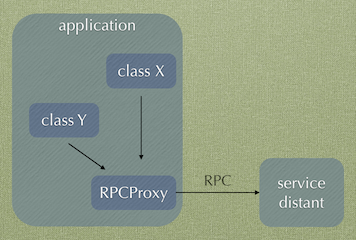
\includegraphics{medias/rpcproxy.png}\\

    Pour implémenter la plomberie liée à RPC, à l'encodage et décodage des
données, et qui sera interne à la classe \texttt{RPCProxy}, on pourra en
vraie grandeur utiliser des outils comme~:

\begin{itemize}
\tightlist
\item
  \href{https://docs.python.org/3/library/xmlrpc.client.html}{\texttt{xmlrpc.client}}
  qui fait partie de la bibliothèque standard~;
\item
  ou, pour JSON, une des nombreuses implémentations qu'un moteur de
  recherche vous exposera si vous cherchez \texttt{python\ rpc\ json},
  comme par exemple
  \href{https://pypi.python.org/pypi/json-rpc/}{\texttt{json-rpc}}.
\end{itemize}

Cela n'est toutefois pas notre sujet ici, et nous nous contenterons,
dans notre code simplifié, d'imprimer un message.

    \hypertarget{une-approche-nauxefve}{%
\subparagraph{Une approche naïve\\\\}\label{une-approche-nauxefve}}

    Se pose donc la question de savoir quelle interface la classe
\texttt{RPCProxy} doit offrir au reste du monde. Dans une première
version naïve on pourrait écrire quelque chose comme~:

    \begin{Verbatim}[commandchars=\\\{\}]
{\color{incolor}In [{\color{incolor}1}]:} \PY{c+c1}{\PYZsh{} la version naïve de la classe RPCProxy}
        
        \PY{k}{class} \PY{n+nc}{RPCProxy}\PY{p}{:}
            
            \PY{k}{def} \PY{n+nf}{\PYZus{}\PYZus{}init\PYZus{}\PYZus{}}\PY{p}{(}\PY{n+nb+bp}{self}\PY{p}{,} \PY{n}{url}\PY{p}{,} \PY{n}{login}\PY{p}{,} \PY{n}{password}\PY{p}{)}\PY{p}{:}
                \PY{n+nb+bp}{self}\PY{o}{.}\PY{n}{url} \PY{o}{=} \PY{n}{url}
                \PY{n+nb+bp}{self}\PY{o}{.}\PY{n}{login} \PY{o}{=} \PY{n}{login}
                \PY{n+nb+bp}{self}\PY{o}{.}\PY{n}{password} \PY{o}{=} \PY{n}{password}
                
            \PY{k}{def} \PY{n+nf}{\PYZus{}forward\PYZus{}call}\PY{p}{(}\PY{n+nb+bp}{self}\PY{p}{,} \PY{n}{functionname}\PY{p}{,} \PY{o}{*}\PY{n}{args}\PY{p}{)}\PY{p}{:}
                \PY{l+s+sd}{\PYZdq{}\PYZdq{}\PYZdq{}}
        \PY{l+s+sd}{        helper method that marshalls and forwards }
        \PY{l+s+sd}{        the function and arguments to the remote end}
        \PY{l+s+sd}{        \PYZdq{}\PYZdq{}\PYZdq{}}
                \PY{n+nb}{print}\PY{p}{(}\PY{n}{f}\PY{l+s+s2}{\PYZdq{}\PYZdq{}\PYZdq{}}\PY{l+s+s2}{Envoi à }\PY{l+s+si}{\PYZob{}self.url\PYZcb{}}
        \PY{l+s+s2}{de la fonction }\PY{l+s+si}{\PYZob{}functionname\PYZcb{}}\PY{l+s+s2}{ \PYZhy{}\PYZhy{} args= }\PY{l+s+si}{\PYZob{}args\PYZcb{}}\PY{l+s+s2}{\PYZdq{}\PYZdq{}\PYZdq{}}\PY{p}{)}
                \PY{k}{return} \PY{l+s+s2}{\PYZdq{}}\PY{l+s+s2}{retour de la fonction }\PY{l+s+s2}{\PYZdq{}} \PY{o}{+} \PY{n}{functionname}
            
            \PY{k}{def} \PY{n+nf}{GetNodes} \PY{p}{(}\PY{n+nb+bp}{self}\PY{p}{,} \PY{o}{*}\PY{n}{args}\PY{p}{)}\PY{p}{:}
                \PY{k}{return} \PY{n+nb+bp}{self}\PY{o}{.}\PY{n}{\PYZus{}forward\PYZus{}call} \PY{p}{(}\PY{l+s+s1}{\PYZsq{}}\PY{l+s+s1}{GetNodes}\PY{l+s+s1}{\PYZsq{}}\PY{p}{,} \PY{o}{*}\PY{n}{args}\PY{p}{)}
            \PY{k}{def} \PY{n+nf}{BookNode} \PY{p}{(}\PY{n+nb+bp}{self}\PY{p}{,} \PY{o}{*}\PY{n}{args}\PY{p}{)}\PY{p}{:}
                \PY{k}{return} \PY{n+nb+bp}{self}\PY{o}{.}\PY{n}{\PYZus{}forward\PYZus{}call} \PY{p}{(}\PY{l+s+s1}{\PYZsq{}}\PY{l+s+s1}{BookNode}\PY{l+s+s1}{\PYZsq{}}\PY{p}{,} \PY{o}{*}\PY{n}{args}\PY{p}{)}
            \PY{k}{def} \PY{n+nf}{ReleaseNode} \PY{p}{(}\PY{n+nb+bp}{self}\PY{p}{,} \PY{o}{*}\PY{n}{args}\PY{p}{)}\PY{p}{:}
                \PY{k}{return} \PY{n+nb+bp}{self}\PY{o}{.}\PY{n}{\PYZus{}forward\PYZus{}call} \PY{p}{(}\PY{l+s+s1}{\PYZsq{}}\PY{l+s+s1}{ReleaseNode}\PY{l+s+s1}{\PYZsq{}}\PY{p}{,} \PY{o}{*}\PY{n}{args}\PY{p}{)}
\end{Verbatim}


    Ainsi l'application utilise la classe de cette façon~:

    \begin{Verbatim}[commandchars=\\\{\}]
{\color{incolor}In [{\color{incolor}2}]:} \PY{c+c1}{\PYZsh{} création d\PYZsq{}une instance de RPCProxy}
        
        \PY{n}{rpc\PYZus{}proxy} \PY{o}{=} \PY{n}{RPCProxy}\PY{p}{(}\PY{n}{url}\PY{o}{=}\PY{l+s+s1}{\PYZsq{}}\PY{l+s+s1}{http://cloud.provider.com/JSONAPI}\PY{l+s+s1}{\PYZsq{}}\PY{p}{,} 
                             \PY{n}{login}\PY{o}{=}\PY{l+s+s1}{\PYZsq{}}\PY{l+s+s1}{dupont}\PY{l+s+s1}{\PYZsq{}}\PY{p}{,}
                             \PY{n}{password}\PY{o}{=}\PY{l+s+s1}{\PYZsq{}}\PY{l+s+s1}{***}\PY{l+s+s1}{\PYZsq{}}\PY{p}{)}
        
        \PY{c+c1}{\PYZsh{} cette partie du code, en tant qu\PYZsq{}utilisateur de l\PYZsq{}API, }
        \PY{c+c1}{\PYZsh{} est supposée connaître les détails}
        \PY{c+c1}{\PYZsh{} des arguments à passer }
        \PY{c+c1}{\PYZsh{} et de comment utiliser les valeurs de retour}
        \PY{n}{nodes\PYZus{}list} \PY{o}{=} \PY{n}{rpc\PYZus{}proxy}\PY{o}{.}\PY{n}{GetNodes} \PY{p}{(} 
            \PY{p}{[} \PY{p}{(}\PY{l+s+s1}{\PYZsq{}}\PY{l+s+s1}{phy\PYZus{}mem}\PY{l+s+s1}{\PYZsq{}}\PY{p}{,} \PY{l+s+s1}{\PYZsq{}}\PY{l+s+s1}{\PYZgt{}=}\PY{l+s+s1}{\PYZsq{}}\PY{p}{,} \PY{l+s+s1}{\PYZsq{}}\PY{l+s+s1}{32G}\PY{l+s+s1}{\PYZsq{}}\PY{p}{)} \PY{p}{]} \PY{p}{)}
        
        \PY{c+c1}{\PYZsh{} réserver un noeud}
        \PY{n}{node\PYZus{}lease} \PY{o}{=} \PY{n}{rpc\PYZus{}proxy}\PY{o}{.}\PY{n}{BookNode} \PY{p}{(}
            \PY{p}{\PYZob{}} \PY{l+s+s1}{\PYZsq{}}\PY{l+s+s1}{id}\PY{l+s+s1}{\PYZsq{}} \PY{p}{:} \PY{l+m+mi}{1002}\PY{p}{,} \PY{l+s+s1}{\PYZsq{}}\PY{l+s+s1}{phy\PYZus{}mem}\PY{l+s+s1}{\PYZsq{}} \PY{p}{:} \PY{l+s+s1}{\PYZsq{}}\PY{l+s+s1}{32G}\PY{l+s+s1}{\PYZsq{}} \PY{p}{\PYZcb{}} \PY{p}{)}
\end{Verbatim}


    \begin{Verbatim}[commandchars=\\\{\}]
Envoi à http://cloud.provider.com/JSONAPI
de la fonction GetNodes -- args= ([('phy\_mem', '>=', '32G')],)
Envoi à http://cloud.provider.com/JSONAPI
de la fonction BookNode -- args= (\{'id': 1002, 'phy\_mem': '32G'\},)

    \end{Verbatim}

    \hypertarget{discussion}{%
\subparagraph{Discussion\\\\}\label{discussion}}

    Quelques commentaires en vrac au sujet de cette approche~:

\begin{itemize}
\tightlist
\item
  l'interface est correcte~; l'objet \texttt{rcp\_proxy} se comporte
  bien comme un proxy, on a donné au programmeur l'illusion complète
  qu'il utilise une classe locale (sauf pour les performances bien
  entendu\ldots{})~;
\item
  la séparation des rôles est raisonnable également, la classe RPCProxy
  n'a pas à connaître le détail de la signature de chaque méthode,
  charge à l'appelant d'utiliser l'API correctement~;
\item
  par contre ce qui cloche, c'est que l'implémentation de la classe
  RPCProxy dépend de la liste des fonctions exposées par l'API~;
  imaginez une API avec 100 ou 200 méthodes, cela donne une dépendance
  assez forte et surtout inutile~;
\item
  enfin, nous avons escamoté la nécessité de faire de RPCProxy un
  \href{http://en.wikipedia.org/wiki/Singleton_pattern}{singleton}, mais
  c'est une toute autre histoire.
\end{itemize}

    \hypertarget{une-approche-plus-subtile}{%
\subparagraph{Une approche plus
subtile\\\\}\label{une-approche-plus-subtile}}

    Pour obtenir une implémentation qui conserve toutes les qualités de la
version naïve, mais sans la nécessité de définir une à une toutes les
fonctions de l'API, on peut tirer profit de \texttt{\_\_getattr\_\_},
comme dans cette deuxième version~:

    \begin{Verbatim}[commandchars=\\\{\}]
{\color{incolor}In [{\color{incolor}3}]:} \PY{c+c1}{\PYZsh{} une deuxième implémentation de RPCProxy}
        
        \PY{k}{class} \PY{n+nc}{RPCProxy}\PY{p}{:}
            
            \PY{k}{def} \PY{n+nf}{\PYZus{}\PYZus{}init\PYZus{}\PYZus{}}\PY{p}{(}\PY{n+nb+bp}{self}\PY{p}{,} \PY{n}{url}\PY{p}{,} \PY{n}{login}\PY{p}{,} \PY{n}{password}\PY{p}{)}\PY{p}{:}
                \PY{n+nb+bp}{self}\PY{o}{.}\PY{n}{url} \PY{o}{=} \PY{n}{url}
                \PY{n+nb+bp}{self}\PY{o}{.}\PY{n}{login} \PY{o}{=} \PY{n}{login}
                \PY{n+nb+bp}{self}\PY{o}{.}\PY{n}{password} \PY{o}{=} \PY{n}{password}
                
            \PY{k}{def} \PY{n+nf}{\PYZus{}\PYZus{}getattr\PYZus{}\PYZus{}}\PY{p}{(}\PY{n+nb+bp}{self}\PY{p}{,} \PY{n}{function}\PY{p}{)}\PY{p}{:}
                \PY{l+s+sd}{\PYZdq{}\PYZdq{}\PYZdq{}}
        \PY{l+s+sd}{        Crée à la volée une méthode sur RPCProxy qui correspond}
        \PY{l+s+sd}{        à la fonction distante \PYZsq{}function\PYZsq{}}
        \PY{l+s+sd}{        \PYZdq{}\PYZdq{}\PYZdq{}}
                \PY{k}{def} \PY{n+nf}{forwarder}\PY{p}{(}\PY{o}{*}\PY{n}{args}\PY{p}{)}\PY{p}{:}
                    \PY{n+nb}{print}\PY{p}{(}\PY{n}{f}\PY{l+s+s2}{\PYZdq{}}\PY{l+s+s2}{Envoi à }\PY{l+s+si}{\PYZob{}self.url\PYZcb{}}\PY{l+s+se}{\PYZbs{}n}\PY{l+s+s2}{de la fonction }\PY{l+s+si}{\PYZob{}function\PYZcb{}}\PY{l+s+s2}{ \PYZhy{}\PYZhy{} args= }\PY{l+s+si}{\PYZob{}args\PYZcb{}}\PY{l+s+s2}{\PYZdq{}}\PY{p}{)}
                    \PY{k}{return} \PY{l+s+s2}{\PYZdq{}}\PY{l+s+s2}{retour de la fonction }\PY{l+s+s2}{\PYZdq{}} \PY{o}{+} \PY{n}{function}
                \PY{k}{return} \PY{n}{forwarder}
\end{Verbatim}


    Qui est cette fois \textbf{totalement découplée} des détails de l'API,
et qu'on peut utiliser exactement comme tout à l'heure~:

    \begin{Verbatim}[commandchars=\\\{\}]
{\color{incolor}In [{\color{incolor}4}]:} \PY{c+c1}{\PYZsh{} création d\PYZsq{}une instance de RPCProxy}
        
        \PY{n}{rpc\PYZus{}proxy} \PY{o}{=} \PY{n}{RPCProxy} \PY{p}{(}\PY{n}{url}\PY{o}{=}\PY{l+s+s1}{\PYZsq{}}\PY{l+s+s1}{http://cloud.provider.com/JSONAPI}\PY{l+s+s1}{\PYZsq{}}\PY{p}{,} 
                              \PY{n}{login}\PY{o}{=}\PY{l+s+s1}{\PYZsq{}}\PY{l+s+s1}{dupont}\PY{l+s+s1}{\PYZsq{}}\PY{p}{,}
                              \PY{n}{password}\PY{o}{=}\PY{l+s+s1}{\PYZsq{}}\PY{l+s+s1}{***}\PY{l+s+s1}{\PYZsq{}}\PY{p}{)}
        
        \PY{c+c1}{\PYZsh{} cette partie du code, en tant qu\PYZsq{}utilisateur de l\PYZsq{}API, }
        \PY{c+c1}{\PYZsh{} est supposée connaître les détails}
        \PY{c+c1}{\PYZsh{} des arguments à passer }
        \PY{c+c1}{\PYZsh{} et de comment utiliser les valeurs de retour}
        \PY{n}{nodes\PYZus{}list} \PY{o}{=} \PY{n}{rpc\PYZus{}proxy}\PY{o}{.}\PY{n}{GetNodes} \PY{p}{(} 
            \PY{p}{[} \PY{p}{(}\PY{l+s+s1}{\PYZsq{}}\PY{l+s+s1}{phy\PYZus{}mem}\PY{l+s+s1}{\PYZsq{}}\PY{p}{,} \PY{l+s+s1}{\PYZsq{}}\PY{l+s+s1}{\PYZgt{}=}\PY{l+s+s1}{\PYZsq{}}\PY{p}{,} \PY{l+s+s1}{\PYZsq{}}\PY{l+s+s1}{32G}\PY{l+s+s1}{\PYZsq{}}\PY{p}{)} \PY{p}{]} \PY{p}{)}
        
        \PY{c+c1}{\PYZsh{} réserver un noeud}
        \PY{n}{node\PYZus{}lease} \PY{o}{=} \PY{n}{rpc\PYZus{}proxy}\PY{o}{.}\PY{n}{BookNode} \PY{p}{(}
            \PY{p}{\PYZob{}} \PY{l+s+s1}{\PYZsq{}}\PY{l+s+s1}{id}\PY{l+s+s1}{\PYZsq{}} \PY{p}{:} \PY{l+m+mi}{1002}\PY{p}{,} \PY{l+s+s1}{\PYZsq{}}\PY{l+s+s1}{phy\PYZus{}mem}\PY{l+s+s1}{\PYZsq{}} \PY{p}{:} \PY{l+s+s1}{\PYZsq{}}\PY{l+s+s1}{32G}\PY{l+s+s1}{\PYZsq{}} \PY{p}{\PYZcb{}} \PY{p}{)}
\end{Verbatim}


    \begin{Verbatim}[commandchars=\\\{\}]
Envoi à http://cloud.provider.com/JSONAPI
de la fonction GetNodes -- args= ([('phy\_mem', '>=', '32G')],)
Envoi à http://cloud.provider.com/JSONAPI
de la fonction BookNode -- args= (\{'id': 1002, 'phy\_mem': '32G'\},)

    \end{Verbatim}
%        
    
    
    

    

    \hypertarget{huxe9ritage}{%
\section{Héritage}\label{huxe9ritage}}

    \hypertarget{compluxe9ment---niveau-basique}{%
\subsection{Complément - niveau
basique}\label{compluxe9ment---niveau-basique}}

    La notion d'héritage, qui fait partie intégrante de la Programmation
Orientée Objet, permet principalement de maximiser la
\textbf{réutilisabilité}.

Nous avons vu dans la vidéo les mécanismes d'héritage \emph{in
abstracto}. Pour résumer très brièvement, on recherche un attribut (pour
notre propos, disons une méthode) à partir d'une instance en cherchant~:

\begin{itemize}
\tightlist
\item
  d'abord dans l'instance elle-même~;
\item
  puis dans la classe de l'instance~;
\item
  puis dans les super-classes de la classe.
\end{itemize}

    L'objet de ce complément est de vous donner, d'un point de vue plus
appliqué, des idées de ce que l'on peut faire ou non avec ce mécanisme.
Le sujet étant assez rabâché par ailleurs, nous nous concentrerons sur
deux points~:

\begin{itemize}
\tightlist
\item
  les pratiques de base utilisées pour la conception de classes, et
  notamment pour bien distinguer \textbf{héritage} et
  \textbf{composition}~;
\item
  nous verrons ensuite, sur des \textbf{exemples extraits de code réel},
  comment ces mécanismes permettent en effet de contribuer à la
  réutilisabilité du code.
\end{itemize}

    \hypertarget{plusieurs-formes-dhuxe9ritage}{%
\subsubsection{Plusieurs formes
d'héritage}\label{plusieurs-formes-dhuxe9ritage}}

    Une méthode héritée peut être rangée dans une de ces trois catégories~:

\begin{itemize}
\tightlist
\item
  \emph{implicite}~: si la classe fille ne définit pas du tout la
  méthode~;
\item
  \emph{redéfinie}~: si on récrit la méthode entièrement~;
\item
  \emph{modifiée}~: si on récrit la méthode dans la classe fille, mais
  en utilisant le code de la classe mère.
\end{itemize}

    Commençons par illustrer tout ceci sur un petit exemple~:

    \begin{Verbatim}[commandchars=\\\{\}]
{\color{incolor}In [{\color{incolor}1}]:} \PY{c+c1}{\PYZsh{} Une classe mère}
        \PY{k}{class} \PY{n+nc}{Fleur}\PY{p}{:}
            \PY{k}{def} \PY{n+nf}{implicite}\PY{p}{(}\PY{n+nb+bp}{self}\PY{p}{)}\PY{p}{:}
                \PY{n+nb}{print}\PY{p}{(}\PY{l+s+s1}{\PYZsq{}}\PY{l+s+s1}{Fleur.implicite}\PY{l+s+s1}{\PYZsq{}}\PY{p}{)}
            \PY{k}{def} \PY{n+nf}{redefinie}\PY{p}{(}\PY{n+nb+bp}{self}\PY{p}{)}\PY{p}{:}
                \PY{n+nb}{print}\PY{p}{(}\PY{l+s+s1}{\PYZsq{}}\PY{l+s+s1}{Fleur.redéfinie}\PY{l+s+s1}{\PYZsq{}}\PY{p}{)}
            \PY{k}{def} \PY{n+nf}{modifiee}\PY{p}{(}\PY{n+nb+bp}{self}\PY{p}{)}\PY{p}{:}
                \PY{n+nb}{print}\PY{p}{(}\PY{l+s+s1}{\PYZsq{}}\PY{l+s+s1}{Fleur.modifiée}\PY{l+s+s1}{\PYZsq{}}\PY{p}{)}
        
        \PY{c+c1}{\PYZsh{} Une classe fille}
        \PY{k}{class} \PY{n+nc}{Rose}\PY{p}{(}\PY{n}{Fleur}\PY{p}{)}\PY{p}{:}
            \PY{c+c1}{\PYZsh{} on ne définit pas implicite}
            \PY{c+c1}{\PYZsh{} on rédéfinit complètement redefinie}
            \PY{k}{def} \PY{n+nf}{redefinie}\PY{p}{(}\PY{n+nb+bp}{self}\PY{p}{)}\PY{p}{:}
                \PY{n+nb}{print}\PY{p}{(}\PY{l+s+s1}{\PYZsq{}}\PY{l+s+s1}{Rose.redefinie}\PY{l+s+s1}{\PYZsq{}}\PY{p}{)}
            \PY{c+c1}{\PYZsh{} on change un peu le comportement de modifiee}
            \PY{k}{def} \PY{n+nf}{modifiee}\PY{p}{(}\PY{n+nb+bp}{self}\PY{p}{)}\PY{p}{:}
                \PY{n}{Fleur}\PY{o}{.}\PY{n}{modifiee}\PY{p}{(}\PY{n+nb+bp}{self}\PY{p}{)}
                \PY{n+nb}{print}\PY{p}{(}\PY{l+s+s1}{\PYZsq{}}\PY{l+s+s1}{Rose.modifiee apres Fleur}\PY{l+s+s1}{\PYZsq{}}\PY{p}{)}
\end{Verbatim}


    On peut à présent créer une instance de Rose et appeler sur cette
instance les trois méthodes.

    \begin{Verbatim}[commandchars=\\\{\}]
{\color{incolor}In [{\color{incolor}2}]:} \PY{c+c1}{\PYZsh{} fille est une instance de Rose}
        \PY{n}{fille} \PY{o}{=} \PY{n}{Rose}\PY{p}{(}\PY{p}{)}
        
        \PY{n}{fille}\PY{o}{.}\PY{n}{implicite}\PY{p}{(}\PY{p}{)}
\end{Verbatim}


    \begin{Verbatim}[commandchars=\\\{\}]
Fleur.implicite

    \end{Verbatim}

    \begin{Verbatim}[commandchars=\\\{\}]
{\color{incolor}In [{\color{incolor}3}]:} \PY{n}{fille}\PY{o}{.}\PY{n}{redefinie}\PY{p}{(}\PY{p}{)}
\end{Verbatim}


    \begin{Verbatim}[commandchars=\\\{\}]
Rose.redefinie

    \end{Verbatim}

    S'agissant des deux premières méthodes, le comportement qu'on observe
est simplement la conséquence de l'algorithme de recherche d'attributs~:
\texttt{implicite} est trouvée dans la classe Fleur et
\texttt{redefinie} est trouvée dans la classe Rose.

    \begin{Verbatim}[commandchars=\\\{\}]
{\color{incolor}In [{\color{incolor}4}]:} \PY{n}{fille}\PY{o}{.}\PY{n}{modifiee}\PY{p}{(}\PY{p}{)}
\end{Verbatim}


    \begin{Verbatim}[commandchars=\\\{\}]
Fleur.modifiée
Rose.modifiee apres Fleur

    \end{Verbatim}

    Pour la troisième méthode, attardons-nous un peu car on voit ici comment
\emph{combiner} facilement le code de la classe mère avec du code
spécifique à la classe fille, en appelant explicitement la méthode de la
classe mère lorsqu'on fait~:

\begin{verbatim}
Fleur.modifiee(self)
\end{verbatim}

    \hypertarget{la-fonction-built-in-super}{%
\subparagraph{\texorpdfstring{La fonction \emph{built-in}
\texttt{super()}}{La fonction built-in super()}}\label{la-fonction-built-in-super}}

    Signalons à ce sujet, pour être exhaustif, l'existence de la
\href{https://docs.python.org/3/library/functions.html\#super}{fonction
\emph{built-in} \texttt{super()}} qui permet de réaliser la même chose
sans nommer explicitement la classe mère, comme on le fait ici~:

    \begin{Verbatim}[commandchars=\\\{\}]
{\color{incolor}In [{\color{incolor}5}]:} \PY{c+c1}{\PYZsh{} Une version allégée de la classe fille, qui utilise super()}
        \PY{k}{class} \PY{n+nc}{Rose}\PY{p}{(}\PY{n}{Fleur}\PY{p}{)}\PY{p}{:}
            \PY{k}{def} \PY{n+nf}{modifiee}\PY{p}{(}\PY{n+nb+bp}{self}\PY{p}{)}\PY{p}{:}
                \PY{n+nb}{super}\PY{p}{(}\PY{p}{)}\PY{o}{.}\PY{n}{modifiee}\PY{p}{(}\PY{p}{)}
                \PY{n+nb}{print}\PY{p}{(}\PY{l+s+s1}{\PYZsq{}}\PY{l+s+s1}{Rose.modifiee apres Fleur}\PY{l+s+s1}{\PYZsq{}}\PY{p}{)}
\end{Verbatim}


    \begin{Verbatim}[commandchars=\\\{\}]
{\color{incolor}In [{\color{incolor}6}]:} \PY{n}{fille} \PY{o}{=} \PY{n}{Rose}\PY{p}{(}\PY{p}{)}
        
        \PY{n}{fille}\PY{o}{.}\PY{n}{modifiee}\PY{p}{(}\PY{p}{)}
\end{Verbatim}


    \begin{Verbatim}[commandchars=\\\{\}]
Fleur.modifiée
Rose.modifiee apres Fleur

    \end{Verbatim}

    On peut envisager d'utiliser \texttt{super()} dans du code très abstrait
où on ne sait pas déterminer statiquement le nom de la classe dont il
est question. Mais, c'est une question de goût évidemment, je recommande
personnellement la première forme, où on qualifie la méthode avec le nom
de la classe mère qu'on souhaite utiliser. En effet, assez souvent~:

\begin{itemize}
\tightlist
\item
  on sait déterminer le nom de la classe dont il est question~;
\item
  ou alors on veut mélanger plusieurs méthodes héritées (via l'héritage
  multiple, dont on va parler dans un prochain complément) et dans ce
  cas \texttt{super()} ne peut rien pour nous.
\end{itemize}

    \hypertarget{huxe9ritage-vs-composition}{%
\subsubsection{\texorpdfstring{Héritage \emph{vs}
Composition}{Héritage vs Composition}}\label{huxe9ritage-vs-composition}}

    Dans le domaine de la conception orientée objet, on fait la différence
entre deux constructions, l'héritage et la composition, qui à une
analyse superficielle peuvent paraître procurer des résultats
similaires, mais qu'il est important de bien distinguer.

Voyons d'abord en quoi consiste la composition et pourquoi le résultat
est voisin~:

    \begin{Verbatim}[commandchars=\\\{\}]
{\color{incolor}In [{\color{incolor}7}]:} \PY{c+c1}{\PYZsh{} Une classe avec qui on n\PYZsq{}aura pas de relation d\PYZsq{}héritage}
        \PY{k}{class} \PY{n+nc}{Tige}\PY{p}{:}
            \PY{k}{def} \PY{n+nf}{implicite}\PY{p}{(}\PY{n+nb+bp}{self}\PY{p}{)}\PY{p}{:}
                \PY{n+nb}{print}\PY{p}{(}\PY{l+s+s1}{\PYZsq{}}\PY{l+s+s1}{Tige.implicite}\PY{l+s+s1}{\PYZsq{}}\PY{p}{)}
            \PY{k}{def} \PY{n+nf}{redefinie}\PY{p}{(}\PY{n+nb+bp}{self}\PY{p}{)}\PY{p}{:}
                \PY{n+nb}{print}\PY{p}{(}\PY{l+s+s1}{\PYZsq{}}\PY{l+s+s1}{Tige.redefinie}\PY{l+s+s1}{\PYZsq{}}\PY{p}{)}
            \PY{k}{def} \PY{n+nf}{modifiee}\PY{p}{(}\PY{n+nb+bp}{self}\PY{p}{)}\PY{p}{:}
                \PY{n+nb}{print}\PY{p}{(}\PY{l+s+s1}{\PYZsq{}}\PY{l+s+s1}{Tige.modifiee}\PY{l+s+s1}{\PYZsq{}}\PY{p}{)}
        
        \PY{c+c1}{\PYZsh{} on n\PYZsq{}hérite pas}
        \PY{c+c1}{\PYZsh{} mais on fait ce qu\PYZsq{}on appelle une composition}
        \PY{c+c1}{\PYZsh{} avec la classe Tige}
        \PY{k}{class} \PY{n+nc}{Rose}\PY{p}{:}
            \PY{c+c1}{\PYZsh{} mais pour chaque objet de la classe Rose}
            \PY{c+c1}{\PYZsh{} on va créer un objet de la classe Tige}
            \PY{c+c1}{\PYZsh{} et le conserver dans un champ}
            \PY{k}{def} \PY{n+nf}{\PYZus{}\PYZus{}init\PYZus{}\PYZus{}}\PY{p}{(}\PY{n+nb+bp}{self}\PY{p}{)}\PY{p}{:}
                \PY{n+nb+bp}{self}\PY{o}{.}\PY{n}{externe} \PY{o}{=} \PY{n}{Tige}\PY{p}{(}\PY{p}{)}
        
            \PY{c+c1}{\PYZsh{} le reste est presque comme tout à l\PYZsq{}heure}
            \PY{c+c1}{\PYZsh{} sauf qu\PYZsq{}il faut definir implicite}
            \PY{k}{def} \PY{n+nf}{implicite}\PY{p}{(}\PY{n+nb+bp}{self}\PY{p}{)}\PY{p}{:}
                \PY{n+nb+bp}{self}\PY{o}{.}\PY{n}{externe}\PY{o}{.}\PY{n}{implicite}\PY{p}{(}\PY{p}{)}
                
            \PY{c+c1}{\PYZsh{} on redéfinit complètement redefinie}
            \PY{k}{def} \PY{n+nf}{redefinie}\PY{p}{(}\PY{n+nb+bp}{self}\PY{p}{)}\PY{p}{:}
                \PY{n+nb}{print}\PY{p}{(}\PY{l+s+s1}{\PYZsq{}}\PY{l+s+s1}{Rose.redefinie}\PY{l+s+s1}{\PYZsq{}}\PY{p}{)}
                
            \PY{k}{def} \PY{n+nf}{modifiee}\PY{p}{(}\PY{n+nb+bp}{self}\PY{p}{)}\PY{p}{:}
                \PY{n+nb+bp}{self}\PY{o}{.}\PY{n}{externe}\PY{o}{.}\PY{n}{modifiee}\PY{p}{(}\PY{p}{)}
                \PY{n+nb}{print}\PY{p}{(}\PY{l+s+s1}{\PYZsq{}}\PY{l+s+s1}{Rose.modifiee apres Tige}\PY{l+s+s1}{\PYZsq{}}\PY{p}{)}
\end{Verbatim}


    \begin{Verbatim}[commandchars=\\\{\}]
{\color{incolor}In [{\color{incolor}8}]:} \PY{c+c1}{\PYZsh{} on obtient ici exactement le même comportement }
        \PY{c+c1}{\PYZsh{} pour les trois sortes de méthodes}
        \PY{n}{fille} \PY{o}{=} \PY{n}{Rose}\PY{p}{(}\PY{p}{)}
        
        \PY{n}{fille}\PY{o}{.}\PY{n}{implicite}\PY{p}{(}\PY{p}{)}
        \PY{n}{fille}\PY{o}{.}\PY{n}{redefinie}\PY{p}{(}\PY{p}{)}
        \PY{n}{fille}\PY{o}{.}\PY{n}{modifiee}\PY{p}{(}\PY{p}{)}
\end{Verbatim}


    \begin{Verbatim}[commandchars=\\\{\}]
Tige.implicite
Rose.redefinie
Tige.modifiee
Rose.modifiee apres Tige

    \end{Verbatim}

    \hypertarget{comment-choisir}{%
\subparagraph{Comment choisir~?}\label{comment-choisir}}

    Alors, quand faut-il utiliser l'héritage et quand faut-il utiliser la
composition~?\\
On arrive ici à la limite de notre cours, il s'agit plus de conception
que de codage à proprement parler, mais pour donner une réponse très
courte à cette question~:

\begin{itemize}
\tightlist
\item
  on utilise l'héritage lorsqu'un objet de la sous-classe \textbf{est
  aussi un} objet de la super-classe (une rose est aussi une fleur)~;
\item
  on utilise la composition lorsqu'un objet de la sous-classe \textbf{a
  une relation avec} un objet de la super-classe (une rose possède une
  tige, mais c'est un autre objet).
\end{itemize}

    \hypertarget{compluxe9ment---niveau-intermuxe9diaire}{%
\subsection{Complément - niveau
intermédiaire}\label{compluxe9ment---niveau-intermuxe9diaire}}

    \hypertarget{des-exemples-de-code}{%
\subsubsection{Des exemples de code}\label{des-exemples-de-code}}

    Sans transition, dans cette section un peu plus prospective, nous vous
avons signalé quelques morceaux de code de la bibliothèque standard qui
utilisent l'héritage. Sans aller nécessairement jusqu'à la lecture de
ces codes, il nous a semblé intéressant de commenter spécifiquement
l'usage qui est fait de l'héritage dans ces bibliothèques.

    \hypertarget{le-module-calendar}{%
\subparagraph{\texorpdfstring{Le module
\texttt{calendar}}{Le module calendar}}\label{le-module-calendar}}

    On trouve dans la bibliothèque standard
\href{https://docs.python.org/3/library/calendar.html}{le module
\texttt{calendar}}. Ce module expose deux classes \texttt{TextCalendar}
et \texttt{HTMLCalendar}. Sans entrer du tout dans le détail, ces deux
classes permettent d'imprimer dans des formats différents le même type
d'informations.

Le point ici est que les concepteurs ont choisi un graphe d'héritage
comme ceci~:

\begin{verbatim}
Calendar
|-- TextCalendar
|-- HTMLCalendar
\end{verbatim}

qui permet de grouper le code concernant la logique dans la classe
\texttt{Calendar}, puis dans les deux sous-classes d'implémenter le type
de sortie qui va bien.

C'est l'utilisateur qui choisit la classe qui lui convient le mieux, et
de cette manière, le maximum de code est partagé entre les deux
classes~; et de plus si vous avez besoin d'une sortie au format, disons
PDF, vous pouvez envisager d'hériter de \texttt{Calendar} et de
n'implémenter que la partie spécifique au format PDF.

C'est un peu le niveau élémentaire de l'héritage.

    \hypertarget{le-module-socketserver}{%
\subparagraph{\texorpdfstring{Le module
\texttt{SocketServer}}{Le module SocketServer}}\label{le-module-socketserver}}

    Toujours dans la bibliothèque standard, le
\href{https://docs.python.org/3/library/socketserver.html}{module
\texttt{SocketServer}} fait un usage beaucoup plus sophistiqué de
l'héritage.

Le module propose une hiérarchie de classes comme ceci~:

    \begin{verbatim}
+------------+
| BaseServer |
+------------+
      |
      v
+-----------+        +------------------+
| TCPServer |------->| UnixStreamServer |
+-----------+        +------------------+
      |
      v
+-----------+        +--------------------+
| UDPServer |------->| UnixDatagramServer |
+-----------+        +--------------------+
\end{verbatim}

    Ici encore notre propos n'est pas d'entrer dans les détails, mais
d'observer le fait que les différents \emph{niveaux d'intelligence} sont
ajoutés les uns aux les autres au fur et à mesure que l'on descend le
graphe d'héritage.

Cette hiérarchie est par ailleurs étendue par le
\href{https://docs.python.org/3/library/http.server.html}{module
\texttt{http.server}} et notamment au travers de la classe
\href{https://docs.python.org/3/library/http.server.html\#http.server.HTTPServer}{\texttt{HTTPServer}}
qui hérite de \texttt{TCPServer}.

    Pour revenir au module \texttt{SocketServer}, j'attire votre attention
dans
\href{https://docs.python.org/3/library/socketserver.html\#examples}{la
page d'exemples} sur
\href{https://docs.python.org/3/library/socketserver.html\#asynchronous-mixins}{cet
exemple en particuler}, où on crée une classe de serveurs multi-threads
(la classe \texttt{ThreadedTCPServer}) par simple héritage multiple
entre \texttt{ThreadingMixIn} et \texttt{TCPServer}. La notion de
\texttt{Mixin} est \href{http://en.wikipedia.org/wiki/Mixin}{décrite
dans cette page Wikipédia} dans laquelle vous pouvez accéder directement
\href{http://en.wikipedia.org/wiki/Mixin\#In_Python}{à la section
consacrée à Python}.


    % Add a bibliography block to the postdoc
    
    
    

%    \include{w6-s3-c3-enums}
%    \include{w6-s3-c4-heritage-typage}
%        
    
    
    

    

    \hypertarget{huxe9ritage-multiple}{%
\section{Héritage multiple}\label{huxe9ritage-multiple}}

    \hypertarget{compluxe9ment---niveau-intermuxe9diaire}{%
\subsection{Complément - niveau
intermédiaire}\label{compluxe9ment---niveau-intermuxe9diaire}}

    \hypertarget{la-classe-object}{%
\subsubsection{\texorpdfstring{La classe
\texttt{object}}{La classe object}}\label{la-classe-object}}

    Le symbole \texttt{object} est une variable prédéfinie (qui donc fait
partie du module \texttt{builtins})~:

    \begin{Verbatim}[commandchars=\\\{\}]
{\color{incolor}In [{\color{incolor}1}]:} \PY{n+nb}{object}
\end{Verbatim}


\begin{Verbatim}[commandchars=\\\{\}]
{\color{outcolor}Out[{\color{outcolor}1}]:} object
\end{Verbatim}
            
    \begin{Verbatim}[commandchars=\\\{\}]
{\color{incolor}In [{\color{incolor}2}]:} \PY{k+kn}{import} \PY{n+nn}{builtins}
        
        \PY{n}{builtins}\PY{o}{.}\PY{n}{object} \PY{o+ow}{is} \PY{n+nb}{object}
\end{Verbatim}


\begin{Verbatim}[commandchars=\\\{\}]
{\color{outcolor}Out[{\color{outcolor}2}]:} True
\end{Verbatim}
            
    La classe \texttt{object} est une classe spéciale~; toutes les classes
en Python héritent de la classe \texttt{object}, même lorsqu'aucun
héritage n'est spécifié~:

    \begin{Verbatim}[commandchars=\\\{\}]
{\color{incolor}In [{\color{incolor}3}]:} \PY{k}{class} \PY{n+nc}{Foo}\PY{p}{:}
            \PY{k}{pass}
        
        \PY{n}{Foo}\PY{o}{.}\PY{n+nv+vm}{\PYZus{}\PYZus{}bases\PYZus{}\PYZus{}}
\end{Verbatim}


\begin{Verbatim}[commandchars=\\\{\}]
{\color{outcolor}Out[{\color{outcolor}3}]:} (object,)
\end{Verbatim}
            
    L'attribut spécial \texttt{\_\_bases\_\_}, comme on le devine, nous
permet d'accéder aux superclasses directes, ici de la classe
\texttt{Foo}.

    En Python moderne, on n'a \textbf{jamais besoin de mentionner}
\texttt{object} dans le code. La raison de sa présence dans les symboles
prédéfinis est liée à l'histoire de Python, et à la distinction que
faisait Python 2 entre classes \emph{old-style} et classes
\emph{new-style}. Nous le mentionnons seulement car on rencontre encore
parfois du code qui fait quelque chose comme~:

    \begin{Verbatim}[commandchars=\\\{\}]
{\color{incolor}In [{\color{incolor}4}]:} \PY{k}{class} \PY{n+nc}{Bar}\PY{p}{(}\PY{n+nb}{object}\PY{p}{)}\PY{p}{:}
            \PY{k}{pass}
\end{Verbatim}


    qui est un reste de Python 2, et que Python 3 accepte uniquement au
titre de la compatibilité.

    \hypertarget{compluxe9ment---niveau-avancuxe9}{%
\subsection{Complément - niveau
avancé}\label{compluxe9ment---niveau-avancuxe9}}

    \hypertarget{rappels}{%
\subsubsection{Rappels}\label{rappels}}

    L'héritage en Python consiste principalement en l'algorithme de
recherche d'un attribut d'une instance~; celui-ci regarde~:

\begin{enumerate}
\def\labelenumi{\arabic{enumi}.}
\tightlist
\item
  d'abord dans l'instance~;
\item
  ensuite dans la classe~;
\item
  ensuite dans les super-classes.
\end{enumerate}

    \hypertarget{ordre-sur-les-super-classes}{%
\subsubsection{Ordre sur les
super-classes}\label{ordre-sur-les-super-classes}}

    Le problème revient donc, pour le dernier point, à définir un
\textbf{ordre} sur l'ensemble des \textbf{super-classes}. On parle bien,
naturellement, de \textbf{toutes} les super-classes, pas seulement
celles dont on hérite directement - en termes savants on dirait qu'on
s'intéresse à la fermeture transitive de la relation d'héritage.

L'algorithme utilisé pour cela depuis la version 2.3 est connu sous le
nom de \textbf{linéarisation C3}. Cet algorithme n'est pas propre à
python, comme vous pourrez le lire dans les références citées dans la
dernière section.

Nous ne décrirons pas ici l'algorithme lui-même dans le détail~; par
contre nous allons~:

\begin{itemize}
\tightlist
\item
  dans un premier temps résumer \textbf{les raisons} qui ont guidé ce
  choix, en décrivant les bonnes propriétés que l'on attend, ainsi que
  les \textbf{limitations} qui en découlent~;
\item
  puis voir l'ordre obtenu sur quelques \textbf{exemples} concrets de
  hiérarchies de classes.
\end{itemize}

Vous trouverez dans les références (voir ci-dessous la dernière section,
``Pour en savoir plus'') des liens vers des documents plus techniques si
vous souhaitez creuser le sujet.

    \hypertarget{les-bonnes-propriuxe9tuxe9s-attendues}{%
\subsubsection{Les bonnes propriétés
attendues}\label{les-bonnes-propriuxe9tuxe9s-attendues}}

    Il y a un certain nombre de bonnes propriétés que l'on attend de cet
algorithme.

    \hypertarget{priorituxe9-au-spuxe9cifique}{%
\subparagraph{Priorité au
spécifique}\label{priorituxe9-au-spuxe9cifique}}

    Lorsqu'une classe A hérite d'une classe B, on s'attend à ce que les
méthodes définies sur A, qui sont en principe plus spécifiques, soient
utilisées de préférence à celles définies sur B.

    \hypertarget{priorituxe9-uxe0-gauche}{%
\subparagraph{Priorité à gauche}\label{priorituxe9-uxe0-gauche}}

    Lorsqu'on utilise l'héritage multiple, on mentionne les classes mères
dans un certain ordre, qui n'est pas anodin. Les classes mentionnées en
premier sont bien entendu celles desquelles on veut hériter en priorité.

    \hypertarget{la-method-resolution-order-mro}{%
\section{La Method Resolution Order
(MRO)}\label{la-method-resolution-order-mro}}

    \hypertarget{de-maniuxe8re-un-peu-plus-formelle}{%
\subparagraph{De manière un peu plus
formelle}\label{de-maniuxe8re-un-peu-plus-formelle}}

    Pour reformuler les deux points ci-dessus, on s'intéresse à la
\texttt{mro} d'une classe O, et on veut avoir les deux bonnes propriétés
suivantes~:

\begin{itemize}
\tightlist
\item
  si O hérite (pas forcément directement) de A qui elle même hérite de
  B, alors A est avant B dans la \texttt{mro} de O~;
\item
  si O hérite (pas forcément directement) de A, qui elle hérite de B,
  puis (pas forcément immédiatement) de C, alors dans la \texttt{mro} A
  est avant B qui est avant C.
\end{itemize}

    \hypertarget{limitations-toutes-les-hiuxe9rarchies-ne-peuvent-pas-uxeatre-traituxe9es}{%
\subparagraph{Limitations~: toutes les hiérarchies ne peuvent pas être
traitées}\label{limitations-toutes-les-hiuxe9rarchies-ne-peuvent-pas-uxeatre-traituxe9es}}

    L'algorithme C3 permet de calculer un ordre sur \(\cal{S}\) qui respecte
toutes ces contraintes, lorsqu'il en existe un.

En effet, dans certains cas on ne peut pas trouver un tel ordre, on le
verra plus bas, mais dans la pratique, il est assez rare de tomber sur
de tels cas pathologiques~; et lorsque cela se produit c'est en général
le signe d'erreurs de conception plus profondes.

    \hypertarget{un-exemple-truxe8s-simple}{%
\subsubsection{Un exemple très simple}\label{un-exemple-truxe8s-simple}}

    On se donne la hiérarchie suivante~:

    \begin{Verbatim}[commandchars=\\\{\}]
{\color{incolor}In [{\color{incolor}5}]:} \PY{k}{class} \PY{n+nc}{LeftTop}\PY{p}{(}\PY{n+nb}{object}\PY{p}{)}\PY{p}{:}
            \PY{k}{def} \PY{n+nf}{attribut}\PY{p}{(}\PY{n+nb+bp}{self}\PY{p}{)}\PY{p}{:} 
                \PY{k}{return} \PY{l+s+s2}{\PYZdq{}}\PY{l+s+s2}{attribut(LeftTop)}\PY{l+s+s2}{\PYZdq{}}
            
        \PY{k}{class} \PY{n+nc}{LeftMiddle}\PY{p}{(}\PY{n}{LeftTop}\PY{p}{)}\PY{p}{:} 
            \PY{k}{pass}
        
        \PY{k}{class} \PY{n+nc}{Left}\PY{p}{(}\PY{n}{LeftMiddle}\PY{p}{)}\PY{p}{:} 
            \PY{k}{pass}
        
        \PY{k}{class} \PY{n+nc}{Middle}\PY{p}{(}\PY{n+nb}{object}\PY{p}{)}\PY{p}{:} 
            \PY{k}{pass}
        
        \PY{k}{class} \PY{n+nc}{Right}\PY{p}{(}\PY{n+nb}{object}\PY{p}{)}\PY{p}{:}
            \PY{k}{def} \PY{n+nf}{attribut}\PY{p}{(}\PY{n+nb+bp}{self}\PY{p}{)}\PY{p}{:} 
                \PY{k}{return} \PY{l+s+s2}{\PYZdq{}}\PY{l+s+s2}{attribut(Right)}\PY{l+s+s2}{\PYZdq{}}
        
        \PY{k}{class} \PY{n+nc}{Class}\PY{p}{(}\PY{n}{Left}\PY{p}{,} \PY{n}{Middle}\PY{p}{,} \PY{n}{Right}\PY{p}{)}\PY{p}{:} 
            \PY{k}{pass}
        
        \PY{n}{instance} \PY{o}{=} \PY{n}{Class}\PY{p}{(}\PY{p}{)}
\end{Verbatim}


    qui donne en version dessinée, avec deux points rouges pour représenter
les deux définitions de la méthode \texttt{attribut}~:

    Les deux règles, telles que nous les avons énoncées en premier lieu
(priorité à gauche, priorité au spécifique) sont un peu contradictoires
ici. En fait, c'est la méthode de \texttt{LeftTop} qui est héritée dans
\texttt{Class}, comme on le voit ici~:

    \begin{Verbatim}[commandchars=\\\{\}]
{\color{incolor}In [{\color{incolor}6}]:} \PY{n}{instance}\PY{o}{.}\PY{n}{attribut}\PY{p}{(}\PY{p}{)} \PY{o}{==} \PY{l+s+s1}{\PYZsq{}}\PY{l+s+s1}{attribut(LeftTop)}\PY{l+s+s1}{\PYZsq{}}
\end{Verbatim}


\begin{Verbatim}[commandchars=\\\{\}]
{\color{outcolor}Out[{\color{outcolor}6}]:} True
\end{Verbatim}
            
    \textbf{Exercice}~: Remarquez qu'ici \texttt{Right} a elle-même un
héritage très simple. À titre d'exercice, modifiez le code ci-dessus
pour faire que \texttt{Right} hérite de la classe \texttt{LeftMiddle}~;
de quelle classe d'après vous est-ce que \texttt{Class} hérite
\texttt{attribut} dans cette configuration~?

    \hypertarget{si-cela-ne-vous-convient-pas}{%
\subparagraph{Si cela ne vous convient
pas}\label{si-cela-ne-vous-convient-pas}}

    C'est une évidence, mais cela va peut-être mieux en le rappelant~: si la
méthode que vous obtenez ``gratuitement'' avec l'héritage n'est pas
celle qui vous convient, vous avez naturellement toujours la possibilité
de la redéfinir, et ainsi d'en \textbf{choisir} une autre. Dans notre
exemple si on préfère la méthode implémentée dans \texttt{Right}, on
définira plutôt la classe \texttt{Class} comme ceci~:

    \begin{Verbatim}[commandchars=\\\{\}]
{\color{incolor}In [{\color{incolor}7}]:} \PY{k}{class} \PY{n+nc}{Class}\PY{p}{(}\PY{n}{Left}\PY{p}{,} \PY{n}{Middle}\PY{p}{,} \PY{n}{Right}\PY{p}{)}\PY{p}{:}
            \PY{c+c1}{\PYZsh{} en redéfinissant explicitement la méthode}
            \PY{c+c1}{\PYZsh{} attribut ici on court\PYZhy{}circuite la mro}
            \PY{c+c1}{\PYZsh{} et on peut appeler explicitement une autre}
            \PY{c+c1}{\PYZsh{} version de attribut()}
            \PY{k}{def} \PY{n+nf}{attribut}\PY{p}{(}\PY{o}{*}\PY{n}{args}\PY{p}{,} \PY{o}{*}\PY{o}{*}\PY{n}{kwds}\PY{p}{)}\PY{p}{:}
                \PY{k}{return} \PY{n}{Right}\PY{o}{.}\PY{n}{attribut}\PY{p}{(}\PY{o}{*}\PY{n}{args}\PY{p}{,} \PY{o}{*}\PY{o}{*}\PY{n}{kwds}\PY{p}{)}
            
        \PY{n}{instance2} \PY{o}{=} \PY{n}{Class}\PY{p}{(}\PY{p}{)}
        \PY{n}{instance2}\PY{o}{.}\PY{n}{attribut}\PY{p}{(}\PY{p}{)}
\end{Verbatim}


\begin{Verbatim}[commandchars=\\\{\}]
{\color{outcolor}Out[{\color{outcolor}7}]:} 'attribut(Right)'
\end{Verbatim}
            
    Ou encore bien entendu, si dans votre contexte vous devez appelez
\textbf{les deux} méthodes dont vous pourriez hériter et les combiner,
vous pouvez le faire aussi, par exemple comme ceci~:

    \begin{Verbatim}[commandchars=\\\{\}]
{\color{incolor}In [{\color{incolor}8}]:} \PY{k}{class} \PY{n+nc}{Class}\PY{p}{(}\PY{n}{Left}\PY{p}{,} \PY{n}{Middle}\PY{p}{,} \PY{n}{Right}\PY{p}{)}\PY{p}{:}
            \PY{c+c1}{\PYZsh{} pour faire un composite des deux méthodes}
            \PY{c+c1}{\PYZsh{} trouvées dans les classes mères}
            \PY{k}{def} \PY{n+nf}{attribut}\PY{p}{(}\PY{o}{*}\PY{n}{args}\PY{p}{,} \PY{o}{*}\PY{o}{*}\PY{n}{kwds}\PY{p}{)}\PY{p}{:}
                \PY{k}{return} \PY{p}{(}  \PY{n}{LeftTop}\PY{o}{.}\PY{n}{attribut}\PY{p}{(}\PY{o}{*}\PY{n}{args}\PY{p}{,} \PY{o}{*}\PY{o}{*}\PY{n}{kwds}\PY{p}{)} 
                        \PY{o}{+} \PY{l+s+s2}{\PYZdq{}}\PY{l+s+s2}{ ** }\PY{l+s+s2}{\PYZdq{}} 
                        \PY{o}{+} \PY{n}{Right}\PY{o}{.}\PY{n}{attribut}\PY{p}{(}\PY{o}{*}\PY{n}{args}\PY{p}{,} \PY{o}{*}\PY{o}{*}\PY{n}{kwds}\PY{p}{)}\PY{p}{)}
            
        \PY{n}{instance3} \PY{o}{=} \PY{n}{Class}\PY{p}{(}\PY{p}{)}
        \PY{n}{instance3}\PY{o}{.}\PY{n}{attribut}\PY{p}{(}\PY{p}{)}
\end{Verbatim}


\begin{Verbatim}[commandchars=\\\{\}]
{\color{outcolor}Out[{\color{outcolor}8}]:} 'attribut(LeftTop) ** attribut(Right)'
\end{Verbatim}
            
    \hypertarget{un-exemple-un-peu-plus-compliquuxe9}{%
\subsubsection{Un exemple un peu plus
compliqué}\label{un-exemple-un-peu-plus-compliquuxe9}}

    Voici un exemple, assez parlant, tiré de la deuxième référence (voir
ci-dessous la dernière section, ``Pour en savoir plus'').

    \begin{Verbatim}[commandchars=\\\{\}]
{\color{incolor}In [{\color{incolor}9}]:} \PY{n}{O} \PY{o}{=} \PY{n+nb}{object}
        \PY{k}{class} \PY{n+nc}{F}\PY{p}{(}\PY{n}{O}\PY{p}{)}\PY{p}{:} \PY{k}{pass}
        \PY{k}{class} \PY{n+nc}{E}\PY{p}{(}\PY{n}{O}\PY{p}{)}\PY{p}{:} \PY{k}{pass}
        \PY{k}{class} \PY{n+nc}{D}\PY{p}{(}\PY{n}{O}\PY{p}{)}\PY{p}{:} \PY{k}{pass}
        \PY{k}{class} \PY{n+nc}{C}\PY{p}{(}\PY{n}{D}\PY{p}{,} \PY{n}{F}\PY{p}{)}\PY{p}{:} \PY{k}{pass}
        \PY{k}{class} \PY{n+nc}{B}\PY{p}{(}\PY{n}{E}\PY{p}{,} \PY{n}{D}\PY{p}{)}\PY{p}{:} \PY{k}{pass}
        \PY{k}{class} \PY{n+nc}{A}\PY{p}{(}\PY{n}{B}\PY{p}{,} \PY{n}{C}\PY{p}{)}\PY{p}{:} \PY{k}{pass}
\end{Verbatim}


    Cette hiérarchie nous donne, en partant de A, l'ordre suivant~:

    \begin{verbatim}
                           6
                          ---
Level 3                  | O |
                       /  ---  \
                      /    |    \
                     /     |     \
                    /      |      \
                  ---     ---    ---
Level 2        2 | E | 4 | D |  | F | 5
                  ---     ---    ---
                   \      / \     /
                    \    /   \   /
                     \  /     \ /
                      ---     ---
Level 1            1 | B |   | C | 3
                      ---     ---
                       \       /
                        \     /
                          ---
Level 0                0 | A |
                          ---
\end{verbatim}

    Que l'on peut calculer, sous l'interpréteur python, avec la méthode
\texttt{mro} sur la classe de départ~:

    \begin{Verbatim}[commandchars=\\\{\}]
{\color{incolor}In [{\color{incolor}10}]:} \PY{n}{A}\PY{o}{.}\PY{n}{mro}\PY{p}{(}\PY{p}{)}
\end{Verbatim}


\begin{Verbatim}[commandchars=\\\{\}]
{\color{outcolor}Out[{\color{outcolor}10}]:} [\_\_main\_\_.A,
          \_\_main\_\_.B,
          \_\_main\_\_.E,
          \_\_main\_\_.C,
          \_\_main\_\_.D,
          \_\_main\_\_.F,
          object]
\end{Verbatim}
            
    \hypertarget{un-exemple-qui-ne-peut-pas-uxeatre-traituxe9}{%
\subsubsection{Un exemple qui ne peut pas être
traité}\label{un-exemple-qui-ne-peut-pas-uxeatre-traituxe9}}

    Voici enfin un exemple de hiérarchie pour laquelle on ne \textbf{peut
pas trouver d'ordre} qui respecte les bonnes propriétés que l'on a vues
tout à l'heure, et qui pour cette raison sera \textbf{rejetée par
l'interpréteur python}. D'abord en version dessinée~:

    \begin{Verbatim}[commandchars=\\\{\}]
{\color{incolor}In [{\color{incolor}11}]:} \PY{c+c1}{\PYZsh{} puis en version code}
         \PY{k}{class} \PY{n+nc}{X}\PY{p}{:} \PY{k}{pass}
         \PY{k}{class} \PY{n+nc}{Y}\PY{p}{:} \PY{k}{pass}
         \PY{k}{class} \PY{n+nc}{XY}\PY{p}{(}\PY{n}{X}\PY{p}{,} \PY{n}{Y}\PY{p}{)}\PY{p}{:} \PY{k}{pass}
         \PY{k}{class} \PY{n+nc}{YX}\PY{p}{(}\PY{n}{Y}\PY{p}{,} \PY{n}{X}\PY{p}{)}\PY{p}{:} \PY{k}{pass}
         
         \PY{c+c1}{\PYZsh{} on essaie de créer une sous\PYZhy{}classe de XY et YX}
         \PY{k}{try}\PY{p}{:}
             \PY{k}{class} \PY{n+nc}{Class}\PY{p}{(}\PY{n}{XY}\PY{p}{,} \PY{n}{YX}\PY{p}{)}\PY{p}{:} \PY{k}{pass} 
         \PY{c+c1}{\PYZsh{} mais ce n\PYZsq{}est pas possible}
         \PY{k}{except} \PY{n+ne}{Exception} \PY{k}{as} \PY{n}{e}\PY{p}{:}
             \PY{n+nb}{print}\PY{p}{(}\PY{n}{f}\PY{l+s+s2}{\PYZdq{}}\PY{l+s+s2}{OOPS, }\PY{l+s+s2}{\PYZob{}}\PY{l+s+s2}{type(e)\PYZcb{}, }\PY{l+s+si}{\PYZob{}e\PYZcb{}}\PY{l+s+s2}{\PYZdq{}}\PY{p}{)}
\end{Verbatim}


    \begin{Verbatim}[commandchars=\\\{\}]
OOPS, <class 'TypeError'>, Cannot create a consistent method resolution
order (MRO) for bases X, Y

    \end{Verbatim}

    \hypertarget{pour-en-savoir-plus}{%
\subsubsection{Pour en savoir plus}\label{pour-en-savoir-plus}}

    \begin{enumerate}
\def\labelenumi{\arabic{enumi}.}
\setcounter{enumi}{-1}
\tightlist
\item
  Un
  \href{http://python-history.blogspot.fr/2010/06/method-resolution-order.html}{blog
  de Guido Van Rossum} qui retrace l'historique des différents essais
  qui ont été faits avant de converger sur le modèle actuel.
\item
  Un \href{https://www.python.org/download/releases/2.3/mro/}{article
  technique} qui décrit le fonctionnement de l'algorithme de calcul de
  la MRO, et donne des exemples.
\item
  L'\href{http://en.wikipedia.org/wiki/C3_linearization}{article de
  Wikipedia} sur l'algorithme C3.
\end{enumerate}


    % Add a bibliography block to the postdoc
    
    
    

%        
    
    
    

    

    \hypertarget{les-attributs}{%
\section{Les attributs}\label{les-attributs}}

    \hypertarget{compluxe9ments---niveau-basique}{%
\subsection{Compléments - niveau
basique}\label{compluxe9ments---niveau-basique}}

    \hypertarget{la-notation-.-et-les-attributs}{%
\subsubsection{\texorpdfstring{La notation \texttt{.} et les
attributs}{La notation . et les attributs}}\label{la-notation-.-et-les-attributs}}

    La notation \texttt{module.variable} que nous avons vue dans la vidéo
est un cas particulier de la notion d'attribut, qui permet d'étendre un
objet, ou si on préfère de lui accrocher des données.

Nous avons déjà rencontré ceci de nombreuses fois à présent, c'est
exactement le même mécanisme d'attribut qui est utilisé pour les
méthodes~; pour le système d'attribut il n'y a pas de différence entre
\texttt{module.variable}, \texttt{module.fonction},
\texttt{objet.methode}, etc.

Nous verrons très bientôt que ce mécanisme est massivement utilisé
également dans les instances de classe.

    \hypertarget{les-fonctions-de-gestion-des-attributs}{%
\subsubsection{Les fonctions de gestion des
attributs}\label{les-fonctions-de-gestion-des-attributs}}

    Pour accéder programmativement aux attributs d'un objet, on dispose des
3 fonctions \emph{built-in} \texttt{getattr}, \texttt{setattr}, et
\texttt{hasattr}, que nous allons illustrer tout de suite.

    \hypertarget{lire-un-attribut}{%
\subparagraph{Lire un attribut}\label{lire-un-attribut}}

    \begin{Verbatim}[commandchars=\\\{\}]
{\color{incolor}In [{\color{incolor}1}]:} \PY{k+kn}{import} \PY{n+nn}{math}
        \PY{c+c1}{\PYZsh{} nous savons lire un attribut comme ceci }
        \PY{c+c1}{\PYZsh{} qui lit l\PYZsq{}attribut de nom \PYZsq{}pi\PYZsq{} dans le module math}
        \PY{n}{math}\PY{o}{.}\PY{n}{pi}
\end{Verbatim}


\begin{Verbatim}[commandchars=\\\{\}]
{\color{outcolor}Out[{\color{outcolor}1}]:} 3.141592653589793
\end{Verbatim}
            
    La
\href{https://docs.python.org/3/library/functions.html\#getattr}{fonction
\emph{built-in} \texttt{getattr}} permet de lire un attribut
programmativement~:

    \begin{Verbatim}[commandchars=\\\{\}]
{\color{incolor}In [{\color{incolor}2}]:} \PY{c+c1}{\PYZsh{} si on part d\PYZsq{}une chaîne qui désigne le nom de l\PYZsq{}attribut}
        \PY{c+c1}{\PYZsh{} la formule équivalente est alors}
        \PY{n+nb}{getattr}\PY{p}{(}\PY{n}{math}\PY{p}{,} \PY{l+s+s1}{\PYZsq{}}\PY{l+s+s1}{pi}\PY{l+s+s1}{\PYZsq{}}\PY{p}{)}
\end{Verbatim}


\begin{Verbatim}[commandchars=\\\{\}]
{\color{outcolor}Out[{\color{outcolor}2}]:} 3.141592653589793
\end{Verbatim}
            
    \begin{Verbatim}[commandchars=\\\{\}]
{\color{incolor}In [{\color{incolor}3}]:} \PY{c+c1}{\PYZsh{} on peut utiliser les attributs avec la plupart des objets}
        \PY{c+c1}{\PYZsh{} ici nous allons le faire sur une fonction}
        \PY{k}{def} \PY{n+nf}{foo}\PY{p}{(}\PY{p}{)}\PY{p}{:} 
            \PY{l+s+s2}{\PYZdq{}}\PY{l+s+s2}{une fonction vide}\PY{l+s+s2}{\PYZdq{}}
            \PY{k}{pass}
        
        \PY{c+c1}{\PYZsh{} on a déjà vu certains attributs des fonctions}
        \PY{n+nb}{print}\PY{p}{(}\PY{n}{f}\PY{l+s+s2}{\PYZdq{}}\PY{l+s+s2}{nom=}\PY{l+s+si}{\PYZob{}foo.\PYZus{}\PYZus{}name\PYZus{}\PYZus{}\PYZcb{}}\PY{l+s+s2}{, docstring=`}\PY{l+s+si}{\PYZob{}foo.\PYZus{}\PYZus{}doc\PYZus{}\PYZus{}\PYZcb{}}\PY{l+s+s2}{`}\PY{l+s+s2}{\PYZdq{}}\PY{p}{)}
\end{Verbatim}


    \begin{Verbatim}[commandchars=\\\{\}]
nom=foo, docstring=`une fonction vide`

    \end{Verbatim}

    \begin{Verbatim}[commandchars=\\\{\}]
{\color{incolor}In [{\color{incolor}4}]:} \PY{c+c1}{\PYZsh{} on peut préciser une valeur par défaut pour le cas où l\PYZsq{}attribut}
        \PY{c+c1}{\PYZsh{} n\PYZsq{}existe pas}
        \PY{n+nb}{getattr}\PY{p}{(}\PY{n}{foo}\PY{p}{,} \PY{l+s+s2}{\PYZdq{}}\PY{l+s+s2}{attribut\PYZus{}inexistant}\PY{l+s+s2}{\PYZdq{}}\PY{p}{,} \PY{l+s+s1}{\PYZsq{}}\PY{l+s+s1}{valeur\PYZus{}par\PYZus{}defaut}\PY{l+s+s1}{\PYZsq{}}\PY{p}{)}
\end{Verbatim}


\begin{Verbatim}[commandchars=\\\{\}]
{\color{outcolor}Out[{\color{outcolor}4}]:} 'valeur\_par\_defaut'
\end{Verbatim}
            
    \hypertarget{uxe9crire-un-attribut}{%
\subparagraph{Écrire un attribut}\label{uxe9crire-un-attribut}}

    \begin{Verbatim}[commandchars=\\\{\}]
{\color{incolor}In [{\color{incolor}5}]:} \PY{c+c1}{\PYZsh{} on peut ajouter un attribut arbitraire (toujours sur l\PYZsq{}objet fonction)}
        \PY{n}{foo}\PY{o}{.}\PY{n}{hauteur} \PY{o}{=} \PY{l+m+mi}{100}
        
        \PY{n}{foo}\PY{o}{.}\PY{n}{hauteur}
\end{Verbatim}


\begin{Verbatim}[commandchars=\\\{\}]
{\color{outcolor}Out[{\color{outcolor}5}]:} 100
\end{Verbatim}
            
    Comme pour la lecture on peut écrire un attribut programmativement avec
la
\href{https://docs.python.org/3/library/functions.html\#setattr}{fonction
\emph{built-in} \texttt{setattr}}~:

    \begin{Verbatim}[commandchars=\\\{\}]
{\color{incolor}In [{\color{incolor}6}]:} \PY{c+c1}{\PYZsh{} écrire un attribut avec setattr}
        \PY{n+nb}{setattr}\PY{p}{(}\PY{n}{foo}\PY{p}{,} \PY{l+s+s2}{\PYZdq{}}\PY{l+s+s2}{largeur}\PY{l+s+s2}{\PYZdq{}}\PY{p}{,} \PY{l+m+mi}{200}\PY{p}{)}
        
        \PY{c+c1}{\PYZsh{} on peut bien sûr le lire indifféremment}
        \PY{c+c1}{\PYZsh{} directement comme ici, ou avec getattr}
        \PY{n}{foo}\PY{o}{.}\PY{n}{largeur}
\end{Verbatim}


\begin{Verbatim}[commandchars=\\\{\}]
{\color{outcolor}Out[{\color{outcolor}6}]:} 200
\end{Verbatim}
            
    \hypertarget{liste-des-attributs}{%
\subparagraph{Liste des attributs}\label{liste-des-attributs}}

    La
\href{https://docs.python.org/3/library/functions.html\#hasattr}{fonction
\emph{built-in} \texttt{hasattr}} permet de savoir si un objet possède
ou pas un attribut~:

    \begin{Verbatim}[commandchars=\\\{\}]
{\color{incolor}In [{\color{incolor}7}]:} \PY{c+c1}{\PYZsh{} pour savoir si un attribut existe}
        \PY{n+nb}{hasattr}\PY{p}{(}\PY{n}{math}\PY{p}{,} \PY{l+s+s1}{\PYZsq{}}\PY{l+s+s1}{pi}\PY{l+s+s1}{\PYZsq{}}\PY{p}{)}
\end{Verbatim}


\begin{Verbatim}[commandchars=\\\{\}]
{\color{outcolor}Out[{\color{outcolor}7}]:} True
\end{Verbatim}
            
    Ce qui peut aussi être retrouvé autrement, avec la
\href{https://docs.python.org/3/library/functions.html\#vars}{fonction
\emph{built-in} \texttt{vars}}~:

    \begin{Verbatim}[commandchars=\\\{\}]
{\color{incolor}In [{\color{incolor}8}]:} \PY{n+nb}{vars}\PY{p}{(}\PY{n}{foo}\PY{p}{)}
\end{Verbatim}


\begin{Verbatim}[commandchars=\\\{\}]
{\color{outcolor}Out[{\color{outcolor}8}]:} \{'hauteur': 100, 'largeur': 200\}
\end{Verbatim}
            
    \hypertarget{sur-quels-objets}{%
\subsubsection{Sur quels objets}\label{sur-quels-objets}}

    Il n'est pas possible d'ajouter des attributs sur les types de base, car
ce sont des classes immuables~:

    \begin{Verbatim}[commandchars=\\\{\}]
{\color{incolor}In [{\color{incolor}9}]:} \PY{k}{for} \PY{n}{builtin\PYZus{}type} \PY{o+ow}{in} \PY{p}{(}\PY{n+nb}{int}\PY{p}{,} \PY{n+nb}{str}\PY{p}{,} \PY{n+nb}{float}\PY{p}{,} \PY{n+nb}{complex}\PY{p}{,} \PY{n+nb}{tuple}\PY{p}{,} \PY{n+nb}{dict}\PY{p}{,} \PY{n+nb}{set}\PY{p}{,} \PY{n+nb}{frozenset}\PY{p}{)}\PY{p}{:}
            \PY{n}{obj} \PY{o}{=} \PY{n}{builtin\PYZus{}type}\PY{p}{(}\PY{p}{)}
            \PY{k}{try}\PY{p}{:} 
                \PY{n}{obj}\PY{o}{.}\PY{n}{foo} \PY{o}{=} \PY{l+s+s1}{\PYZsq{}}\PY{l+s+s1}{bar}\PY{l+s+s1}{\PYZsq{}}
            \PY{k}{except} \PY{n+ne}{AttributeError} \PY{k}{as} \PY{n}{e}\PY{p}{:} 
                \PY{n+nb}{print}\PY{p}{(}\PY{n}{f}\PY{l+s+s2}{\PYZdq{}}\PY{l+s+si}{\PYZob{}builtin\PYZus{}type.\PYZus{}\PYZus{}name\PYZus{}\PYZus{}:\PYZgt{}10\PYZcb{}}\PY{l+s+s2}{ → exception }\PY{l+s+s2}{\PYZob{}}\PY{l+s+s2}{type(e)\PYZcb{} \PYZhy{} }\PY{l+s+si}{\PYZob{}e\PYZcb{}}\PY{l+s+s2}{\PYZdq{}}\PY{p}{)}
\end{Verbatim}


    \begin{Verbatim}[commandchars=\\\{\}]
       int → exception <class 'AttributeError'> - 'int' object has no attribute 'foo'
       str → exception <class 'AttributeError'> - 'str' object has no attribute 'foo'
     float → exception <class 'AttributeError'> - 'float' object has no attribute 'foo'
   complex → exception <class 'AttributeError'> - 'complex' object has no attribute 'foo'
     tuple → exception <class 'AttributeError'> - 'tuple' object has no attribute 'foo'
      dict → exception <class 'AttributeError'> - 'dict' object has no attribute 'foo'
       set → exception <class 'AttributeError'> - 'set' object has no attribute 'foo'
 frozenset → exception <class 'AttributeError'> - 'frozenset' object has no attribute 'foo'

    \end{Verbatim}

    C'est par contre possible sur virtuellement tout le reste, et notamment
là où c'est très utile, c'est-à-dire pour ce qui nous concerne sur les~:

\begin{itemize}
\tightlist
\item
  modules
\item
  packages
\item
  fonctions
\item
  classes
\item
  instances
\end{itemize}


    % Add a bibliography block to the postdoc
    
    
    

%    \include{w6-s5-c2-namepsaces}
%        \hypertarget{compluxe9ment---niveau-avancuxe9}{%
\subsection{Complément - niveau
avancé}\label{compluxe9ment---niveau-avancuxe9}}

    \hypertarget{impluxe9menter-un-ituxe9rateur-de-permutations}{%
\subsubsection{Implémenter un itérateur de
permutations}\label{impluxe9menter-un-ituxe9rateur-de-permutations}}

    Dans ce complément nous allons nous amuser à implémenter une
fonctionnalité qui est déjà disponible dans le module
\texttt{itertools}.

    \hypertarget{cest-quoi-duxe9juxe0-les-permutations}{%
\subparagraph{C'est quoi déjà les
permutations~?}\label{cest-quoi-duxe9juxe0-les-permutations}}

    En guise de rappel, l'ensemble des permutations d'un ensemble fini
correspond à toutes les façons d'ordonner ses éléments~; si l'ensemble
est de cardinal \(n\), il possède \(n!\) permutations~: on a \(n\)
façons de choisir le premier élément, \(n-1\) façons de choisir le
second, etc.\\

    Un itérateur sur les permutations est disponible au travers du module
standard \texttt{itertools}. Cependant il nous a semblé intéressant de
vous montrer comment nous pourrions écrire nous-mêmes cette
fonctionnalité, de manière relativement simple.\\

    Pour illustrer le concept, voici à quoi ressemblent les 6 permutations
d'un ensemble à trois éléments~:

    \begin{Verbatim}[commandchars=\\\{\}]
{\color{incolor}In [{\color{incolor}1}]:} \PY{k+kn}{from} \PY{n+nn}{itertools} \PY{k}{import} \PY{n}{permutations}
\end{Verbatim}


    \begin{Verbatim}[commandchars=\\\{\}]
{\color{incolor}In [{\color{incolor}2}]:} \PY{n+nb}{set} \PY{o}{=} \PY{p}{\PYZob{}}\PY{l+m+mi}{1}\PY{p}{,} \PY{l+m+mi}{2}\PY{p}{,} \PY{l+m+mi}{3}\PY{p}{\PYZcb{}}
        
        \PY{k}{for} \PY{n}{p} \PY{o+ow}{in} \PY{n}{permutations}\PY{p}{(}\PY{n+nb}{set}\PY{p}{)}\PY{p}{:}
            \PY{n+nb}{print}\PY{p}{(}\PY{n}{p}\PY{p}{)}
\end{Verbatim}


    \begin{Verbatim}[commandchars=\\\{\}]
(1, 2, 3)
(1, 3, 2)
(2, 1, 3)
(2, 3, 1)
(3, 1, 2)
(3, 2, 1)

    \end{Verbatim}

    \hypertarget{une-impluxe9mentation}{%
\subparagraph{Une implémentation\\\\}\label{une-impluxe9mentation}}

    Voici une implémentation possible pour un itérateur de permutations~:

    \begin{Verbatim}[commandchars=\\\{\}]
{\color{incolor}In [{\color{incolor}3}]:} \PY{k}{class} \PY{n+nc}{Permutations}\PY{p}{:}
            \PY{l+s+sd}{\PYZdq{}\PYZdq{}\PYZdq{}}
        \PY{l+s+sd}{    Un itérateur qui énumère les permutations de n}
        \PY{l+s+sd}{    sous la forme d\PYZsq{}une liste d\PYZsq{}indices commençant à 0}
        \PY{l+s+sd}{    \PYZdq{}\PYZdq{}\PYZdq{}}
            \PY{k}{def} \PY{n+nf}{\PYZus{}\PYZus{}init\PYZus{}\PYZus{}}\PY{p}{(}\PY{n+nb+bp}{self}\PY{p}{,} \PY{n}{n}\PY{p}{)}\PY{p}{:}
                \PY{c+c1}{\PYZsh{} le constructeur bien sûr ne fait (presque) rien}
                \PY{n+nb+bp}{self}\PY{o}{.}\PY{n}{n} \PY{o}{=} \PY{n}{n}
                \PY{c+c1}{\PYZsh{} au fur et à mesure des itérations}
                \PY{c+c1}{\PYZsh{} le compteur va aller de 0 à n\PYZhy{}1}
                \PY{c+c1}{\PYZsh{} puis retour à 0 et comme ça en boucle sans fin}
                \PY{n+nb+bp}{self}\PY{o}{.}\PY{n}{counter} \PY{o}{=} \PY{l+m+mi}{0}
                \PY{c+c1}{\PYZsh{} on se contente d\PYZsq{}allouer un iterateur de rang n\PYZhy{}1}
                \PY{c+c1}{\PYZsh{} si bien qu\PYZsq{}une fois qu\PYZsq{}on a fini de construire}
                \PY{c+c1}{\PYZsh{} l\PYZsq{}objet d\PYZsq{}ordre n on a n objets Permutations en tout}
                \PY{k}{if} \PY{n}{n} \PY{o}{\PYZgt{}}\PY{o}{=} \PY{l+m+mi}{2}\PY{p}{:}
                    \PY{n+nb+bp}{self}\PY{o}{.}\PY{n}{subiterator} \PY{o}{=} \PY{n}{Permutations}\PY{p}{(}\PY{n}{n}\PY{o}{\PYZhy{}}\PY{l+m+mi}{1}\PY{p}{)}
        
            \PY{c+c1}{\PYZsh{} pour satisfaire le protocole d\PYZsq{}itération}
            \PY{k}{def} \PY{n+nf}{\PYZus{}\PYZus{}iter\PYZus{}\PYZus{}}\PY{p}{(}\PY{n+nb+bp}{self}\PY{p}{)}\PY{p}{:}
                \PY{k}{return} \PY{n+nb+bp}{self}
        
            \PY{c+c1}{\PYZsh{} c\PYZsq{}est ici bien sûr que se fait tout le travail}
            \PY{k}{def} \PY{n+nf}{\PYZus{}\PYZus{}next\PYZus{}\PYZus{}}\PY{p}{(}\PY{n+nb+bp}{self}\PY{p}{)}\PY{p}{:}
                \PY{c+c1}{\PYZsh{} pour n == 1}
                \PY{c+c1}{\PYZsh{} le travail est très simple}
                \PY{k}{if} \PY{n+nb+bp}{self}\PY{o}{.}\PY{n}{n} \PY{o}{==} \PY{l+m+mi}{1}\PY{p}{:}
                    \PY{c+c1}{\PYZsh{} on doit renvoyer une fois la liste [0]}
                    \PY{c+c1}{\PYZsh{} car les indices commencent à 0}
                    \PY{k}{if} \PY{n+nb+bp}{self}\PY{o}{.}\PY{n}{counter} \PY{o}{==} \PY{l+m+mi}{0}\PY{p}{:} 
                        \PY{n+nb+bp}{self}\PY{o}{.}\PY{n}{counter} \PY{o}{+}\PY{o}{=} \PY{l+m+mi}{1}
                        \PY{k}{return} \PY{p}{[}\PY{l+m+mi}{0}\PY{p}{]}
                    \PY{c+c1}{\PYZsh{} et ensuite c\PYZsq{}est terminé}
                    \PY{k}{else}\PY{p}{:}
                        \PY{k}{raise} \PY{n+ne}{StopIteration}
        
                \PY{c+c1}{\PYZsh{} pour n \PYZgt{}= 2}
                \PY{c+c1}{\PYZsh{} lorsque counter est nul,}
                \PY{c+c1}{\PYZsh{} on traite la permutation d\PYZsq{}ordre n\PYZhy{}1 suivante}
                \PY{c+c1}{\PYZsh{} si next() lève StopIteration on n\PYZsq{}a qu\PYZsq{}à laisser passer}
                \PY{c+c1}{\PYZsh{} car en effet c\PYZsq{}est qu\PYZsq{}on a terminé}
                \PY{k}{if} \PY{n+nb+bp}{self}\PY{o}{.}\PY{n}{counter} \PY{o}{==} \PY{l+m+mi}{0}\PY{p}{:}
                    \PY{n+nb+bp}{self}\PY{o}{.}\PY{n}{subsequence} \PY{o}{=} \PY{n+nb}{next}\PY{p}{(}\PY{n+nb+bp}{self}\PY{o}{.}\PY{n}{subiterator}\PY{p}{)}
                \PY{c+c1}{\PYZsh{}}
                \PY{c+c1}{\PYZsh{} on insère alors n\PYZhy{}1 (car les indices commencent à 0)}
                \PY{c+c1}{\PYZsh{} successivement dans la sous\PYZhy{}sequence}
                \PY{c+c1}{\PYZsh{}}
                \PY{c+c1}{\PYZsh{} naivement on écrirait}
                \PY{c+c1}{\PYZsh{} result = self.subsequence[0:self.counter] \PYZbs{}}
                \PY{c+c1}{\PYZsh{}    + [self.n \PYZhy{} 1] \PYZbs{}}
                \PY{c+c1}{\PYZsh{}    + self.subsequence[self.counter:self.n\PYZhy{}1]}
                \PY{c+c1}{\PYZsh{} mais c\PYZsq{}est mettre le nombre le plus élevé en premier}
                \PY{c+c1}{\PYZsh{} et donc à itérer les permutations dans le mauvais ordre,}
                \PY{c+c1}{\PYZsh{} en commençant par la fin}
                \PY{c+c1}{\PYZsh{}}
                \PY{c+c1}{\PYZsh{} donc on fait plutôt une symétrie}
                \PY{c+c1}{\PYZsh{} pour insérer en commençant par la fin}
                \PY{n}{cutter} \PY{o}{=} \PY{n+nb+bp}{self}\PY{o}{.}\PY{n}{n}\PY{o}{\PYZhy{}}\PY{l+m+mi}{1} \PY{o}{\PYZhy{}} \PY{n+nb+bp}{self}\PY{o}{.}\PY{n}{counter}
                \PY{n}{result} \PY{o}{=} \PY{n+nb+bp}{self}\PY{o}{.}\PY{n}{subsequence}\PY{p}{[}\PY{l+m+mi}{0}\PY{p}{:}\PY{n}{cutter}\PY{p}{]} \PY{o}{+} \PY{p}{[}\PY{n+nb+bp}{self}\PY{o}{.}\PY{n}{n} \PY{o}{\PYZhy{}} \PY{l+m+mi}{1}\PY{p}{]} \PYZbs{}
                         \PY{o}{+} \PY{n+nb+bp}{self}\PY{o}{.}\PY{n}{subsequence}\PY{p}{[}\PY{n}{cutter}\PY{p}{:}\PY{n+nb+bp}{self}\PY{o}{.}\PY{n}{n}\PY{o}{\PYZhy{}}\PY{l+m+mi}{1}\PY{p}{]}
                \PY{c+c1}{\PYZsh{} }
                \PY{c+c1}{\PYZsh{} on n\PYZsq{}oublie pas de maintenir le compteur et de}
                \PY{c+c1}{\PYZsh{} le remettre à zéro tous les n tours}
                \PY{n+nb+bp}{self}\PY{o}{.}\PY{n}{counter} \PY{o}{=} \PY{p}{(}\PY{n+nb+bp}{self}\PY{o}{.}\PY{n}{counter}\PY{o}{+}\PY{l+m+mi}{1}\PY{p}{)} \PY{o}{\PYZpc{}} \PY{n+nb+bp}{self}\PY{o}{.}\PY{n}{n}
                \PY{k}{return} \PY{n}{result}
        
            \PY{c+c1}{\PYZsh{} la longeur de cet itérateur est connue}
            \PY{k}{def} \PY{n+nf}{\PYZus{}\PYZus{}len\PYZus{}\PYZus{}}\PY{p}{(}\PY{n+nb+bp}{self}\PY{p}{)}\PY{p}{:}
                \PY{k+kn}{import} \PY{n+nn}{math}
                \PY{k}{return} \PY{n}{math}\PY{o}{.}\PY{n}{factorial}\PY{p}{(}\PY{n+nb+bp}{self}\PY{o}{.}\PY{n}{n}\PY{p}{)}
\end{Verbatim}


    Ce qu'on a essayé d'expliquer dans les commentaires, c'est qu'on procède
en fin de compte par récurrence. Un objet \texttt{Permutations} de rang
\texttt{n} possède un sous-itérateur de rang \texttt{n-1} qu'on crée
dans le constructeur. Ensuite l'objet de rang \texttt{n} va faire
successivement (c'est-à-dire à chaque appel de \texttt{next()})~:

\begin{itemize}
\item
  appel \emph{0}~:

  \begin{itemize}
  \tightlist
  \item
    demander à son sous-itérateur une permutation de rang \texttt{n-1}
    (en lui envoyant \texttt{next}),
  \item
    la stocker dans l'objet de rang \texttt{n}, ce sera utilisé par les
    \emph{n} premier appels,
  \item
    et construire une liste de taille \texttt{n} en insérant
    \texttt{n-1} à la fin de la séquence de taille \texttt{n-1},
  \end{itemize}
\item
  appel \emph{1}~:

  \begin{itemize}
  \tightlist
  \item
    insérer \texttt{n-1} dans la même séquence de rang \texttt{n-1} mais
    cette fois 1 cran avant la fin,
  \end{itemize}
\item
  \ldots{}
\item
  appel \emph{n-1}~:

  \begin{itemize}
  \tightlist
  \item
    insérer \texttt{n-1} au début de la séquence de rang \texttt{n-1},
  \end{itemize}
\item
  appel \emph{n}~:

  \begin{itemize}
  \tightlist
  \item
    refaire \texttt{next()} sur le sous-itérateur pour traiter une
    nouvelle sous-séquence,
  \item
    la stocker dans l'objet de rang \texttt{n}, comme à l'appel
    \emph{0}, pour ce bloc de n appels,
  \item
    et construire la permutation en insérant \emph{n-1} à la fin, comme
    à l'appel 0,
  \end{itemize}
\item
  \ldots{}
\end{itemize}

    On voit donc le caractère cyclique d'ordre \emph{n} qui est matérialisé
par \texttt{counter}, que l'on incrémente à chaque boucle mais modulo
\emph{n} - notez d'ailleurs que pour ce genre de comportement on dispose
aussi de \texttt{itertools.cycle} comme on le verra dans une deuxième
version, mais pour l'instant j'ai préféré ne pas l'utiliser pour ne pas
tout embrouiller ;)\\

La terminaison se gère très simplement, car une fois que l'on a traité
toutes les séquences d'ordre \emph{n-1} eh bien on a fini, on n'a même
pas besoin de lever StopIteration explicitement, sauf bien sûr dans le
cas \emph{n=1}.\\

Le seul point un peu délicat, si on veut avoir les permutations dans le
``bon'' ordre, consiste à commencer à insérer \texttt{n-1} par la droite
(la fin de la sous-séquence).

    \hypertarget{discussion}{%
\subparagraph{Discussion\\\\}\label{discussion}}

    Il existe certainement des tas d'autres façons de faire bien entendu. Le
point important ici, et qui donne toute sa puissance à la notion
d'itérateur, c'est \textbf{qu'à aucun moment on ne construit} une liste
ou une séquence quelconque de \textbf{n! termes}.

C'est une erreur fréquente chez les débutants que de calculer une telle
liste dans le constructeur, mais procéder de cette façon c'est aller
exactement à l'opposé de ce pourquoi les itérateurs ont été conçus~; au
contraire, on veut éviter à tout prix le coût d'une telle construction.

On peut le voir sur un code qui n'utiliserait que les 20 premières
valeurs de l'itérateur, vous constatez que ce code est immédiat~:

    \begin{Verbatim}[commandchars=\\\{\}]
{\color{incolor}In [{\color{incolor}4}]:} \PY{k}{def} \PY{n+nf}{show\PYZus{}first\PYZus{}items}\PY{p}{(}\PY{n}{iterable}\PY{p}{,} \PY{n}{nb\PYZus{}items}\PY{p}{)}\PY{p}{:}
            \PY{l+s+sd}{\PYZdq{}\PYZdq{}\PYZdq{}}
        \PY{l+s+sd}{    montre les \PYZlt{}nb\PYZus{}items\PYZgt{} premiers items de iterable}
        \PY{l+s+sd}{    \PYZdq{}\PYZdq{}\PYZdq{}}
            \PY{n+nb}{print}\PY{p}{(}\PY{n}{f}\PY{l+s+s2}{\PYZdq{}}\PY{l+s+s2}{Il y a }\PY{l+s+s2}{\PYZob{}}\PY{l+s+s2}{len(iterable)\PYZcb{} items dans l}\PY{l+s+s2}{\PYZsq{}}\PY{l+s+s2}{itérable}\PY{l+s+s2}{\PYZdq{}}\PY{p}{)}
            \PY{k}{for} \PY{n}{i}\PY{p}{,} \PY{n}{item} \PY{o+ow}{in} \PY{n+nb}{enumerate}\PY{p}{(}\PY{n}{iterable}\PY{p}{)}\PY{p}{:}
                \PY{n+nb}{print}\PY{p}{(}\PY{n}{item}\PY{p}{)}
                \PY{k}{if} \PY{n}{i} \PY{o}{\PYZgt{}}\PY{o}{=} \PY{n}{nb\PYZus{}items}\PY{p}{:}
                    \PY{n+nb}{print}\PY{p}{(}\PY{l+s+s1}{\PYZsq{}}\PY{l+s+s1}{....}\PY{l+s+s1}{\PYZsq{}}\PY{p}{)}
                    \PY{k}{break}
\end{Verbatim}


    \begin{Verbatim}[commandchars=\\\{\}]
{\color{incolor}In [{\color{incolor}5}]:} \PY{n}{show\PYZus{}first\PYZus{}items}\PY{p}{(}\PY{n}{Permutations}\PY{p}{(}\PY{l+m+mi}{12}\PY{p}{)}\PY{p}{,} \PY{l+m+mi}{20}\PY{p}{)}
\end{Verbatim}


    \begin{Verbatim}[commandchars=\\\{\}]
Il y a 479001600 items dans l'itérable
[0, 1, 2, 3, 4, 5, 6, 7, 8, 9, 10, 11]
[0, 1, 2, 3, 4, 5, 6, 7, 8, 9, 11, 10]
[0, 1, 2, 3, 4, 5, 6, 7, 8, 11, 9, 10]
[0, 1, 2, 3, 4, 5, 6, 7, 11, 8, 9, 10]
[0, 1, 2, 3, 4, 5, 6, 11, 7, 8, 9, 10]
[0, 1, 2, 3, 4, 5, 11, 6, 7, 8, 9, 10]
[0, 1, 2, 3, 4, 11, 5, 6, 7, 8, 9, 10]
[0, 1, 2, 3, 11, 4, 5, 6, 7, 8, 9, 10]
[0, 1, 2, 11, 3, 4, 5, 6, 7, 8, 9, 10]
[0, 1, 11, 2, 3, 4, 5, 6, 7, 8, 9, 10]
[0, 11, 1, 2, 3, 4, 5, 6, 7, 8, 9, 10]
[11, 0, 1, 2, 3, 4, 5, 6, 7, 8, 9, 10]
[0, 1, 2, 3, 4, 5, 6, 7, 8, 10, 9, 11]
[0, 1, 2, 3, 4, 5, 6, 7, 8, 10, 11, 9]
[0, 1, 2, 3, 4, 5, 6, 7, 8, 11, 10, 9]
[0, 1, 2, 3, 4, 5, 6, 7, 11, 8, 10, 9]
[0, 1, 2, 3, 4, 5, 6, 11, 7, 8, 10, 9]
[0, 1, 2, 3, 4, 5, 11, 6, 7, 8, 10, 9]
[0, 1, 2, 3, 4, 11, 5, 6, 7, 8, 10, 9]
[0, 1, 2, 3, 11, 4, 5, 6, 7, 8, 10, 9]
[0, 1, 2, 11, 3, 4, 5, 6, 7, 8, 10, 9]
{\ldots}

    \end{Verbatim}

    Ce tableau vous montre par ailleurs sous un autre angle comment
fonctionne l'algorithme, si vous observez le \texttt{11} qui balaie en
diagonale les 12 premières lignes, puis les 12 suivantes, etc..

    \hypertarget{ultimes-amuxe9liorations}{%
\subparagraph{Ultimes améliorations\\\\}\label{ultimes-amuxe9liorations}}

    Dernières remarques, sur des améliorations possibles - mais tout à fait
optionnelles~:

\begin{itemize}
\tightlist
\item
  le lecteur attentif aura remarqué qu'au lieu d'un entier
  \texttt{counter} on aurait pu profitablement utiliser une instance de
  \texttt{itertools.cycle}, ce qui aurait eu l'avantage d'être plus
  clair sur le propos de ce compteur~;
\item
  aussi dans le même mouvement, au lieu de se livrer à la gymnastique
  qui calcule \texttt{cutter} à partir de \texttt{counter}, on pourrait
  dès le départ créer dans le cycle les bonnes valeurs en commençant à
  \texttt{n-1}.
\end{itemize}

    C'est ce qu'on a fait dans cette deuxième version~; après avoir enlevé
la logorrhée de commentaires ça redevient presque lisible ;)

    \begin{Verbatim}[commandchars=\\\{\}]
{\color{incolor}In [{\color{incolor}6}]:} \PY{k+kn}{import} \PY{n+nn}{itertools}
        
        \PY{k}{class} \PY{n+nc}{Permutations2}\PY{p}{:}
            \PY{l+s+sd}{\PYZdq{}\PYZdq{}\PYZdq{}}
        \PY{l+s+sd}{    Un itérateur qui énumère les permutations de n}
        \PY{l+s+sd}{    sous la forme d\PYZsq{}une liste d\PYZsq{}indices commençant à 0}
        \PY{l+s+sd}{    \PYZdq{}\PYZdq{}\PYZdq{}}
            \PY{k}{def} \PY{n+nf}{\PYZus{}\PYZus{}init\PYZus{}\PYZus{}}\PY{p}{(}\PY{n+nb+bp}{self}\PY{p}{,} \PY{n}{n}\PY{p}{)}\PY{p}{:}
                \PY{n+nb+bp}{self}\PY{o}{.}\PY{n}{n} \PY{o}{=} \PY{n}{n}
                \PY{c+c1}{\PYZsh{} on commence à insérer à la fin }
                \PY{n+nb+bp}{self}\PY{o}{.}\PY{n}{cycle} \PY{o}{=} \PY{n}{itertools}\PY{o}{.}\PY{n}{cycle}\PY{p}{(}\PY{n+nb}{list}\PY{p}{(}\PY{n+nb}{range}\PY{p}{(}\PY{n}{n}\PY{p}{)}\PY{p}{)}\PY{p}{[}\PY{p}{:}\PY{p}{:}\PY{o}{\PYZhy{}}\PY{l+m+mi}{1}\PY{p}{]}\PY{p}{)}
                \PY{k}{if} \PY{n}{n} \PY{o}{\PYZgt{}}\PY{o}{=} \PY{l+m+mi}{2}\PY{p}{:}
                    \PY{n+nb+bp}{self}\PY{o}{.}\PY{n}{subiterator} \PY{o}{=} \PY{n}{Permutations2}\PY{p}{(}\PY{n}{n}\PY{o}{\PYZhy{}}\PY{l+m+mi}{1}\PY{p}{)}
                \PY{c+c1}{\PYZsh{} pour savoir quand terminer le cas n==1}
                \PY{k}{if} \PY{n}{n} \PY{o}{==} \PY{l+m+mi}{1}\PY{p}{:}
                    \PY{n+nb+bp}{self}\PY{o}{.}\PY{n}{done} \PY{o}{=} \PY{k+kc}{False}
        
            \PY{k}{def} \PY{n+nf}{\PYZus{}\PYZus{}iter\PYZus{}\PYZus{}}\PY{p}{(}\PY{n+nb+bp}{self}\PY{p}{)}\PY{p}{:}
                \PY{k}{return} \PY{n+nb+bp}{self}
        
            \PY{k}{def} \PY{n+nf}{\PYZus{}\PYZus{}next\PYZus{}\PYZus{}}\PY{p}{(}\PY{n+nb+bp}{self}\PY{p}{)}\PY{p}{:}
                \PY{n}{cutter} \PY{o}{=} \PY{n+nb}{next}\PY{p}{(}\PY{n+nb+bp}{self}\PY{o}{.}\PY{n}{cycle}\PY{p}{)}
        
                \PY{c+c1}{\PYZsh{} quand n==1 on a toujours la même valeur 0}
                \PY{k}{if} \PY{n+nb+bp}{self}\PY{o}{.}\PY{n}{n} \PY{o}{==} \PY{l+m+mi}{1}\PY{p}{:}
                    \PY{k}{if} \PY{o+ow}{not} \PY{n+nb+bp}{self}\PY{o}{.}\PY{n}{done}\PY{p}{:}
                        \PY{n+nb+bp}{self}\PY{o}{.}\PY{n}{done} \PY{o}{=} \PY{k+kc}{True}
                        \PY{k}{return} \PY{p}{[}\PY{l+m+mi}{0}\PY{p}{]}
                    \PY{k}{else}\PY{p}{:}
                        \PY{k}{raise} \PY{n+ne}{StopIteration}
        
                \PY{c+c1}{\PYZsh{} au début de chaque séquence de n appels}
                \PY{c+c1}{\PYZsh{} il faut appeler une nouvelle sous\PYZhy{}séquence}
                \PY{k}{if} \PY{n}{cutter} \PY{o}{==} \PY{n+nb+bp}{self}\PY{o}{.}\PY{n}{n}\PY{o}{\PYZhy{}}\PY{l+m+mi}{1}\PY{p}{:}
                    \PY{n+nb+bp}{self}\PY{o}{.}\PY{n}{subsequence} \PY{o}{=} \PY{n+nb}{next}\PY{p}{(}\PY{n+nb+bp}{self}\PY{o}{.}\PY{n}{subiterator}\PY{p}{)}
                \PY{c+c1}{\PYZsh{} dans laquelle on insére n\PYZhy{}1}
                \PY{k}{return} \PY{n+nb+bp}{self}\PY{o}{.}\PY{n}{subsequence}\PY{p}{[}\PY{l+m+mi}{0}\PY{p}{:}\PY{n}{cutter}\PY{p}{]} \PY{o}{+} \PY{p}{[}\PY{n+nb+bp}{self}\PY{o}{.}\PY{n}{n}\PY{o}{\PYZhy{}}\PY{l+m+mi}{1}\PY{p}{]} \PYZbs{}
                         \PY{o}{+} \PY{n+nb+bp}{self}\PY{o}{.}\PY{n}{subsequence}\PY{p}{[}\PY{n}{cutter}\PY{p}{:}\PY{n+nb+bp}{self}\PY{o}{.}\PY{n}{n}\PY{o}{\PYZhy{}}\PY{l+m+mi}{1}\PY{p}{]}
        
            \PY{c+c1}{\PYZsh{} la longeur de cet itérateur est connue}
            \PY{k}{def} \PY{n+nf}{\PYZus{}\PYZus{}len\PYZus{}\PYZus{}}\PY{p}{(}\PY{n+nb+bp}{self}\PY{p}{)}\PY{p}{:}
                \PY{k+kn}{import} \PY{n+nn}{math}
                \PY{k}{return} \PY{n}{math}\PY{o}{.}\PY{n}{factorial}\PY{p}{(}\PY{n+nb+bp}{self}\PY{o}{.}\PY{n}{n}\PY{p}{)}
\end{Verbatim}


    \begin{Verbatim}[commandchars=\\\{\}]
{\color{incolor}In [{\color{incolor}7}]:} \PY{n}{show\PYZus{}first\PYZus{}items}\PY{p}{(}\PY{n}{Permutations2}\PY{p}{(}\PY{l+m+mi}{5}\PY{p}{)}\PY{p}{,} \PY{l+m+mi}{20}\PY{p}{)}
\end{Verbatim}


    \begin{Verbatim}[commandchars=\\\{\}]
Il y a 120 items dans l'itérable
[0, 1, 2, 3, 4]
[0, 1, 2, 4, 3]
[0, 1, 4, 2, 3]
[0, 4, 1, 2, 3]
[4, 0, 1, 2, 3]
[0, 1, 3, 2, 4]
[0, 1, 3, 4, 2]
[0, 1, 4, 3, 2]
[0, 4, 1, 3, 2]
[4, 0, 1, 3, 2]
[0, 3, 1, 2, 4]
[0, 3, 1, 4, 2]
[0, 3, 4, 1, 2]
[0, 4, 3, 1, 2]
[4, 0, 3, 1, 2]
[3, 0, 1, 2, 4]
[3, 0, 1, 4, 2]
[3, 0, 4, 1, 2]
[3, 4, 0, 1, 2]
[4, 3, 0, 1, 2]
[0, 2, 1, 3, 4]
{\ldots}

    \end{Verbatim}


    Il me semble intéressant de montrer une autre façon, plus simple,
d'écrire un itérateur de permutations, à base cette fois de générateurs;
c'est un tout petit peu une digression par rapport au cours qui est sur
la conception d'itérateurs et d'itérables. Ça va nous permettre surtout
de réviser la notion de \texttt{yield\ from}.

    On commence par une version très rustique qui fait des impressions~:

    \begin{Verbatim}[commandchars=\\\{\}]
{\color{incolor}In [{\color{incolor}8}]:} \PY{c+c1}{\PYZsh{} pour simplifier ici on suppose que l\PYZsq{}entrée est une vraie liste}
        \PY{c+c1}{\PYZsh{} que l\PYZsq{}on va ainsi pouvoir modifier par effets de bord}
        \PY{k}{def} \PY{n+nf}{gen\PYZus{}perm1}\PY{p}{(}\PY{n}{subject}\PY{p}{,} \PY{n}{k}\PY{o}{=}\PY{l+m+mi}{0}\PY{p}{)}\PY{p}{:}
            \PY{k}{if} \PY{n}{k} \PY{o}{==} \PY{n+nb}{len}\PY{p}{(}\PY{n}{subject}\PY{p}{)}\PY{p}{:}
                \PY{c+c1}{\PYZsh{} cette version hyper rustique se contente de faire une impression}
                \PY{n+nb}{print}\PY{p}{(}\PY{n}{subject}\PY{p}{)}
            \PY{k}{else}\PY{p}{:}
                \PY{k}{for} \PY{n}{i} \PY{o+ow}{in} \PY{n+nb}{range}\PY{p}{(}\PY{n}{k}\PY{p}{,} \PY{n+nb}{len}\PY{p}{(}\PY{n}{subject}\PY{p}{)}\PY{p}{)}\PY{p}{:}
                    \PY{c+c1}{\PYZsh{} on échange }
                    \PY{n}{subject}\PY{p}{[}\PY{n}{k}\PY{p}{]}\PY{p}{,} \PY{n}{subject}\PY{p}{[}\PY{n}{i}\PY{p}{]} \PY{o}{=} \PY{n}{subject}\PY{p}{[}\PY{n}{i}\PY{p}{]}\PY{p}{,} \PY{n}{subject}\PY{p}{[}\PY{n}{k}\PY{p}{]}
                    \PY{n}{gen\PYZus{}perm1}\PY{p}{(}\PY{n}{subject}\PY{p}{,} \PY{n}{k}\PY{o}{+}\PY{l+m+mi}{1}\PY{p}{)}
                    \PY{c+c1}{\PYZsh{} on remet comme c\PYZsq{}était pour le prochain échange}
                    \PY{n}{subject}\PY{p}{[}\PY{n}{k}\PY{p}{]}\PY{p}{,} \PY{n}{subject}\PY{p}{[}\PY{n}{i}\PY{p}{]} \PY{o}{=} \PY{n}{subject}\PY{p}{[}\PY{n}{i}\PY{p}{]}\PY{p}{,} \PY{n}{subject}\PY{p}{[}\PY{n}{k}\PY{p}{]}
\end{Verbatim}


    \begin{Verbatim}[commandchars=\\\{\}]
{\color{incolor}In [{\color{incolor}9}]:} \PY{n}{gen\PYZus{}perm1}\PY{p}{(}\PY{p}{[}\PY{l+s+s1}{\PYZsq{}}\PY{l+s+s1}{a}\PY{l+s+s1}{\PYZsq{}}\PY{p}{,} \PY{l+s+s1}{\PYZsq{}}\PY{l+s+s1}{b}\PY{l+s+s1}{\PYZsq{}}\PY{p}{,} \PY{l+s+s1}{\PYZsq{}}\PY{l+s+s1}{c}\PY{l+s+s1}{\PYZsq{}}\PY{p}{,} \PY{l+s+s1}{\PYZsq{}}\PY{l+s+s1}{d}\PY{l+s+s1}{\PYZsq{}}\PY{p}{]}\PY{p}{)}
\end{Verbatim}


    \begin{Verbatim}[commandchars=\\\{\}]
['a', 'b', 'c', 'd']
['a', 'b', 'd', 'c']
['a', 'c', 'b', 'd']
['a', 'c', 'd', 'b']
['a', 'd', 'c', 'b']
['a', 'd', 'b', 'c']
['b', 'a', 'c', 'd']
['b', 'a', 'd', 'c']
['b', 'c', 'a', 'd']
['b', 'c', 'd', 'a']
['b', 'd', 'c', 'a']
['b', 'd', 'a', 'c']
['c', 'b', 'a', 'd']
['c', 'b', 'd', 'a']
['c', 'a', 'b', 'd']
['c', 'a', 'd', 'b']
['c', 'd', 'a', 'b']
['c', 'd', 'b', 'a']
['d', 'b', 'c', 'a']
['d', 'b', 'a', 'c']
['d', 'c', 'b', 'a']
['d', 'c', 'a', 'b']
['d', 'a', 'c', 'b']
['d', 'a', 'b', 'c']

    \end{Verbatim}

    Très bien, mais on ne veut pas imprimer, on veut itérer. On pourrait se
dire, il me suffit de remplacer \texttt{print} par \texttt{yield}.
Essayons cela~:

    \begin{Verbatim}[commandchars=\\\{\}]
{\color{incolor}In [{\color{incolor}10}]:} \PY{c+c1}{\PYZsh{} pour simplifier ici on suppose que l\PYZsq{}entrée est une vraie liste}
         \PY{c+c1}{\PYZsh{} que l\PYZsq{}on va ainsi pouvoir modifier par effets de bord}
         \PY{k}{def} \PY{n+nf}{gen\PYZus{}perm2}\PY{p}{(}\PY{n}{subject}\PY{p}{,} \PY{n}{k}\PY{o}{=}\PY{l+m+mi}{0}\PY{p}{)}\PY{p}{:}
             \PY{k}{if} \PY{n}{k} \PY{o}{==} \PY{n+nb}{len}\PY{p}{(}\PY{n}{subject}\PY{p}{)}\PY{p}{:}
                 \PY{c+c1}{\PYZsh{} cette version hyper rustique se contente de faire une impression}
                 \PY{k}{yield} \PY{n}{subject}
             \PY{k}{else}\PY{p}{:}
                 \PY{k}{for} \PY{n}{i} \PY{o+ow}{in} \PY{n+nb}{range}\PY{p}{(}\PY{n}{k}\PY{p}{,} \PY{n+nb}{len}\PY{p}{(}\PY{n}{subject}\PY{p}{)}\PY{p}{)}\PY{p}{:}
                     \PY{c+c1}{\PYZsh{} on échange }
                     \PY{n}{subject}\PY{p}{[}\PY{n}{k}\PY{p}{]}\PY{p}{,} \PY{n}{subject}\PY{p}{[}\PY{n}{i}\PY{p}{]} \PY{o}{=} \PY{n}{subject}\PY{p}{[}\PY{n}{i}\PY{p}{]}\PY{p}{,} \PY{n}{subject}\PY{p}{[}\PY{n}{k}\PY{p}{]}
                     \PY{n}{gen\PYZus{}perm2}\PY{p}{(}\PY{n}{subject}\PY{p}{,} \PY{n}{k}\PY{o}{+}\PY{l+m+mi}{1}\PY{p}{)}
                     \PY{c+c1}{\PYZsh{} on remet comme c\PYZsq{}était pour le prochain échange}
                     \PY{n}{subject}\PY{p}{[}\PY{n}{k}\PY{p}{]}\PY{p}{,} \PY{n}{subject}\PY{p}{[}\PY{n}{i}\PY{p}{]} \PY{o}{=} \PY{n}{subject}\PY{p}{[}\PY{n}{i}\PY{p}{]}\PY{p}{,} \PY{n}{subject}\PY{p}{[}\PY{n}{k}\PY{p}{]}
\end{Verbatim}


    \begin{Verbatim}[commandchars=\\\{\}]
{\color{incolor}In [{\color{incolor}11}]:} \PY{k}{for} \PY{n}{perm} \PY{o+ow}{in} \PY{n}{gen\PYZus{}perm2}\PY{p}{(}\PY{p}{[}\PY{l+s+s1}{\PYZsq{}}\PY{l+s+s1}{a}\PY{l+s+s1}{\PYZsq{}}\PY{p}{,} \PY{l+s+s1}{\PYZsq{}}\PY{l+s+s1}{b}\PY{l+s+s1}{\PYZsq{}}\PY{p}{,} \PY{l+s+s1}{\PYZsq{}}\PY{l+s+s1}{c}\PY{l+s+s1}{\PYZsq{}}\PY{p}{,} \PY{l+s+s1}{\PYZsq{}}\PY{l+s+s1}{d}\PY{l+s+s1}{\PYZsq{}}\PY{p}{]}\PY{p}{)}\PY{p}{:}
             \PY{n+nb}{print}\PY{p}{(}\PY{n}{perm}\PY{p}{)}
\end{Verbatim}


    On est exactement dans le cas où il nous faut utiliser
\texttt{yield\ from}. En effet lorsqu'on appelle
\texttt{gen\_perm(subject,\ k+1)} ici, ce qu'on obtient en retour c'est
maintenant un objet générateur. Pour faire ce qu'on cherche à faire il
nous faut bien utiliser cet objet générateur, et pour cela on utilise
\texttt{yield\ from}.

    \begin{Verbatim}[commandchars=\\\{\}]
{\color{incolor}In [{\color{incolor}12}]:} \PY{c+c1}{\PYZsh{} pour simplifier ici on suppose que l\PYZsq{}entrée est une vraie liste}
         \PY{c+c1}{\PYZsh{} que l\PYZsq{}on va ainsi pouvoir modifier par effets de bord}
         \PY{k}{def} \PY{n+nf}{gen\PYZus{}perm3}\PY{p}{(}\PY{n}{subject}\PY{p}{,} \PY{n}{k}\PY{o}{=}\PY{l+m+mi}{0}\PY{p}{)}\PY{p}{:}
             \PY{k}{if} \PY{n}{k} \PY{o}{==} \PY{n+nb}{len}\PY{p}{(}\PY{n}{subject}\PY{p}{)}\PY{p}{:}
                 \PY{c+c1}{\PYZsh{} cette version hyper rustique se contente de faire une impression}
                 \PY{k}{yield} \PY{n}{subject}
             \PY{k}{else}\PY{p}{:}
                 \PY{k}{for} \PY{n}{i} \PY{o+ow}{in} \PY{n+nb}{range}\PY{p}{(}\PY{n}{k}\PY{p}{,} \PY{n+nb}{len}\PY{p}{(}\PY{n}{subject}\PY{p}{)}\PY{p}{)}\PY{p}{:}
                     \PY{c+c1}{\PYZsh{} on échange }
                     \PY{n}{subject}\PY{p}{[}\PY{n}{k}\PY{p}{]}\PY{p}{,} \PY{n}{subject}\PY{p}{[}\PY{n}{i}\PY{p}{]} \PY{o}{=} \PY{n}{subject}\PY{p}{[}\PY{n}{i}\PY{p}{]}\PY{p}{,} \PY{n}{subject}\PY{p}{[}\PY{n}{k}\PY{p}{]}
                     \PY{k}{yield from} \PY{n}{gen\PYZus{}perm3}\PY{p}{(}\PY{n}{subject}\PY{p}{,} \PY{n}{k}\PY{o}{+}\PY{l+m+mi}{1}\PY{p}{)}
                     \PY{c+c1}{\PYZsh{} on remet comme c\PYZsq{}était pour le prochain échange}
                     \PY{n}{subject}\PY{p}{[}\PY{n}{k}\PY{p}{]}\PY{p}{,} \PY{n}{subject}\PY{p}{[}\PY{n}{i}\PY{p}{]} \PY{o}{=} \PY{n}{subject}\PY{p}{[}\PY{n}{i}\PY{p}{]}\PY{p}{,} \PY{n}{subject}\PY{p}{[}\PY{n}{k}\PY{p}{]}
\end{Verbatim}


    \begin{Verbatim}[commandchars=\\\{\}]
{\color{incolor}In [{\color{incolor}13}]:} \PY{k}{for} \PY{n}{perm} \PY{o+ow}{in} \PY{n}{gen\PYZus{}perm3}\PY{p}{(}\PY{p}{[}\PY{l+s+s1}{\PYZsq{}}\PY{l+s+s1}{a}\PY{l+s+s1}{\PYZsq{}}\PY{p}{,} \PY{l+s+s1}{\PYZsq{}}\PY{l+s+s1}{b}\PY{l+s+s1}{\PYZsq{}}\PY{p}{,} \PY{l+s+s1}{\PYZsq{}}\PY{l+s+s1}{c}\PY{l+s+s1}{\PYZsq{}}\PY{p}{,} \PY{l+s+s1}{\PYZsq{}}\PY{l+s+s1}{d}\PY{l+s+s1}{\PYZsq{}}\PY{p}{]}\PY{p}{)}\PY{p}{:}
             \PY{n+nb}{print}\PY{p}{(}\PY{n}{perm}\PY{p}{)}
\end{Verbatim}


    \begin{Verbatim}[commandchars=\\\{\}]
['a', 'b', 'c', 'd']
['a', 'b', 'd', 'c']
['a', 'c', 'b', 'd']
['a', 'c', 'd', 'b']
['a', 'd', 'c', 'b']
['a', 'd', 'b', 'c']
['b', 'a', 'c', 'd']
['b', 'a', 'd', 'c']
['b', 'c', 'a', 'd']
['b', 'c', 'd', 'a']
['b', 'd', 'c', 'a']
['b', 'd', 'a', 'c']
['c', 'b', 'a', 'd']
['c', 'b', 'd', 'a']
['c', 'a', 'b', 'd']
['c', 'a', 'd', 'b']
['c', 'd', 'a', 'b']
['c', 'd', 'b', 'a']
['d', 'b', 'c', 'a']
['d', 'b', 'a', 'c']
['d', 'c', 'b', 'a']
['d', 'c', 'a', 'b']
['d', 'a', 'c', 'b']
['d', 'a', 'b', 'c']

    \end{Verbatim}
%       
    
    
    

    

    \hypertarget{context-managers-et-exceptions}{%
\section{\texorpdfstring{\emph{Context managers} et
exceptions}{Context managers et exceptions}}\label{context-managers-et-exceptions}}

    \hypertarget{compluxe9ment---niveau-intermuxe9diaire}{%
\subsection{Complément - niveau
intermédiaire}\label{compluxe9ment---niveau-intermuxe9diaire}}

    On a vu jusqu'ici dans la vidéo comment écrire un context manager; on a
vu notamment qu'il était bon pour la méthode \texttt{\_\_exit\_\_()} de
retourner \texttt{False}, de façon à ce que l'exception soit propagée à
l'instruction \texttt{with}:

    \begin{Verbatim}[commandchars=\\\{\},frame=single,framerule=0.3mm,rulecolor=\color{cellframecolor}]
{\color{incolor}In [{\color{incolor}1}]:} \PY{k+kn}{import} \PY{n+nn}{time}
        
        \PY{k}{class} \PY{n+nc}{Timer1}\PY{p}{:}
            \PY{k}{def} \PY{n+nf}{\PYZus{}\PYZus{}enter\PYZus{}\PYZus{}}\PY{p}{(}\PY{n+nb+bp}{self}\PY{p}{)}\PY{p}{:}
                \PY{n+nb}{print}\PY{p}{(}\PY{l+s+s2}{\PYZdq{}}\PY{l+s+s2}{Entering Timer1}\PY{l+s+s2}{\PYZdq{}}\PY{p}{)}
                \PY{n+nb+bp}{self}\PY{o}{.}\PY{n}{start} \PY{o}{=} \PY{n}{time}\PY{o}{.}\PY{n}{time}\PY{p}{(}\PY{p}{)}
                \PY{k}{return} \PY{n+nb+bp}{self}
            
            \PY{c+c1}{\PYZsh{} en règle générale on se contente de propager l\PYZsq{}exception }
            \PY{c+c1}{\PYZsh{} à l\PYZsq{}instruction with englobante}
            \PY{k}{def} \PY{n+nf}{\PYZus{}\PYZus{}exit\PYZus{}\PYZus{}}\PY{p}{(}\PY{n+nb+bp}{self}\PY{p}{,} \PY{o}{*}\PY{n}{args}\PY{p}{)}\PY{p}{:}
                \PY{n+nb}{print}\PY{p}{(}\PY{n}{f}\PY{l+s+s2}{\PYZdq{}}\PY{l+s+s2}{Total duration }\PY{l+s+s2}{\PYZob{}}\PY{l+s+s2}{time.time()\PYZhy{}self.start:2f\PYZcb{}}\PY{l+s+s2}{\PYZdq{}}\PY{p}{)}
        
                \PY{c+c1}{\PYZsh{} et pour cela il suffit que \PYZus{}\PYZus{}exit\PYZus{}\PYZus{} retourne False}
                \PY{k}{return} \PY{k+kc}{False}
\end{Verbatim}


    Ainsi si le corps de l'instruction lève une exception, celle-ci est
propagée :

    \begin{Verbatim}[commandchars=\\\{\},frame=single,framerule=0.3mm,rulecolor=\color{cellframecolor}]
{\color{incolor}In [{\color{incolor}2}]:} \PY{k+kn}{import} \PY{n+nn}{time}
        \PY{k}{try}\PY{p}{:}
            \PY{k}{with} \PY{n}{Timer1}\PY{p}{(}\PY{p}{)}\PY{p}{:}
                \PY{n}{time}\PY{o}{.}\PY{n}{sleep}\PY{p}{(}\PY{l+m+mf}{0.5}\PY{p}{)}
                \PY{l+m+mi}{1}\PY{o}{/}\PY{l+m+mi}{0}
        \PY{k}{except} \PY{n+ne}{Exception} \PY{k}{as} \PY{n}{exc}\PY{p}{:}
            \PY{c+c1}{\PYZsh{} on va bien recevoir cette exception}
            \PY{n+nb}{print}\PY{p}{(}\PY{n}{f}\PY{l+s+s2}{\PYZdq{}}\PY{l+s+s2}{OOPS \PYZhy{}\PYZgt{} }\PY{l+s+s2}{\PYZob{}}\PY{l+s+s2}{type(exc)\PYZcb{}}\PY{l+s+s2}{\PYZdq{}}\PY{p}{)}
\end{Verbatim}


    \begin{Verbatim}[commandchars=\\\{\},frame=single,framerule=0.3mm,rulecolor=\color{cellframecolor}]
Entering Timer1
Total duration 0.500135
OOPS -> <class 'ZeroDivisionError'>
\end{Verbatim}

    À la toute première itération de la boucle, on fait une division par 0
qui lève l'exception \texttt{ZeroDivisionError}, qui passe bien à
l'appelant.

Il est important, lorsqu'on conçoit un context manager, de bien
\textbf{propager} les exceptions qui ne sont pas liées au fonctionnement
attendu du context manager. Par exemple un objet de type fichier va par
exemple devoir attraper les exceptions liées à la fin du fichier, mais
doit par contre laisser passer une exception comme
\texttt{ZeroDivisionError}.

    \hypertarget{les-paramuxe8tres-de-__exit__}{%
\subsubsection{\texorpdfstring{Les paramètres de
\texttt{\_\_exit\_\_}}{Les paramètres de \_\_exit\_\_}}\label{les-paramuxe8tres-de-__exit__}}

    Si on a besoin de filtrer entre les exceptions - c'est-à-dire en laisser
passer certaines et pas d'autres - il nous faut quelque chose de plus
pour pouvoir faire le tri. Comme
\href{https://docs.python.org/3/reference/datamodel.html\#with-statement-context-managers}{vous
pouvez le retrouver ici}, la méthode \texttt{\_\_exit\_\_} reçoit trois
arguments~:

\begin{Shaded}
\begin{Highlighting}[frame=lines,framerule=0.6mm,rulecolor=\color{asisframecolor}]
\KeywordTok{def} \FunctionTok{__exit__}\NormalTok{(}\VariableTok{self}\NormalTok{, exc_type, exc_value, traceback):}
\end{Highlighting}
\end{Shaded}

\begin{itemize}
\tightlist
\item
  si l'on sort du bloc \texttt{with} sans qu'une exception soit levée,
  ces trois arguments valent \texttt{None};
\item
  par contre si une exception est levée, ils permettent d'accéder
  respectivement au type, à la valeur de l'exception, et à l'état de la
  pile lorsque l'exception est levée.
\end{itemize}

    Pour illustrer cela, écrivons une nouvelle version de \texttt{Timer} qui
filtre, disons, l'exception \texttt{ZeroDivisionError} que je choisis au
hasard, c'est uniquement pour illustrer le mécanisme.

    \begin{Verbatim}[commandchars=\\\{\},frame=single,framerule=0.3mm,rulecolor=\color{cellframecolor}]
{\color{incolor}In [{\color{incolor}3}]:} \PY{c+c1}{\PYZsh{} une deuxième version de Timer}
        \PY{c+c1}{\PYZsh{} qui propage toutes les exceptions sauf \PYZsq{}OSError\PYZsq{}}
        
        \PY{k}{class} \PY{n+nc}{Timer2}\PY{p}{:}
            \PY{k}{def} \PY{n+nf}{\PYZus{}\PYZus{}enter\PYZus{}\PYZus{}}\PY{p}{(}\PY{n+nb+bp}{self}\PY{p}{)}\PY{p}{:}
                \PY{n+nb}{print}\PY{p}{(}\PY{l+s+s2}{\PYZdq{}}\PY{l+s+s2}{Entering Timer1}\PY{l+s+s2}{\PYZdq{}}\PY{p}{)}
                \PY{n+nb+bp}{self}\PY{o}{.}\PY{n}{start} \PY{o}{=} \PY{n}{time}\PY{o}{.}\PY{n}{time}\PY{p}{(}\PY{p}{)}
                \PY{c+c1}{\PYZsh{} rappel : le retour de \PYZus{}\PYZus{}enter\PYZus{}\PYZus{} est ce qui est passé}
                \PY{c+c1}{\PYZsh{} à la clause `as` du `with`}
                \PY{k}{return} \PY{n+nb+bp}{self}
            
            \PY{k}{def} \PY{n+nf}{\PYZus{}\PYZus{}exit\PYZus{}\PYZus{}}\PY{p}{(}\PY{n+nb+bp}{self}\PY{p}{,} \PY{n}{exc\PYZus{}type}\PY{p}{,} \PY{n}{exc\PYZus{}value}\PY{p}{,} \PY{n}{traceback}\PY{p}{)}\PY{p}{:}
                \PY{k}{if} \PY{n}{exc\PYZus{}type} \PY{o+ow}{is} \PY{k+kc}{None}\PY{p}{:}
                    \PY{c+c1}{\PYZsh{} pas d\PYZsq{}exception levée dans le corps du \PYZsq{}with\PYZsq{}}
                    \PY{n+nb}{print}\PY{p}{(}\PY{n}{f}\PY{l+s+s2}{\PYZdq{}}\PY{l+s+s2}{Total duration }\PY{l+s+s2}{\PYZob{}}\PY{l+s+s2}{time.time()\PYZhy{}self.start:2f\PYZcb{}}\PY{l+s+s2}{\PYZdq{}}\PY{p}{)}
                    \PY{c+c1}{\PYZsh{} dans ce cas la valeur de retour n\PYZsq{}est pas utilisée}
                \PY{k}{else}\PY{p}{:}
                    \PY{c+c1}{\PYZsh{} il y a eu une exception de type \PYZsq{}exc\PYZus{}type\PYZsq{}}
                    \PY{k}{if} \PY{n}{exc\PYZus{}type} \PY{o+ow}{in} \PY{p}{(}\PY{n+ne}{ZeroDivisionError}\PY{p}{,}\PY{p}{)} \PY{p}{:}
                        \PY{n+nb}{print}\PY{p}{(}\PY{l+s+s2}{\PYZdq{}}\PY{l+s+s2}{on étouffe}\PY{l+s+s2}{\PYZdq{}}\PY{p}{)}
                        \PY{c+c1}{\PYZsh{} on peut l\PYZsq{}étouffer en retournant True}
                        \PY{k}{return} \PY{k+kc}{True}
                    \PY{k}{else}\PY{p}{:}
                        \PY{n+nb}{print}\PY{p}{(}\PY{n}{f}\PY{l+s+s2}{\PYZdq{}}\PY{l+s+s2}{OOPS : on propage l}\PY{l+s+s2}{\PYZsq{}}\PY{l+s+s2}{exception }\PY{l+s+s2}{\PYZdq{}}
                              \PY{n}{f}\PY{l+s+s2}{\PYZdq{}}\PY{l+s+si}{\PYZob{}exc\PYZus{}type\PYZcb{}}\PY{l+s+s2}{ \PYZhy{} }\PY{l+s+si}{\PYZob{}exc\PYZus{}value\PYZcb{}}\PY{l+s+s2}{\PYZdq{}}\PY{p}{)}
                        \PY{c+c1}{\PYZsh{} et pour ça il suffit... de ne rien faire du tout}
                        \PY{c+c1}{\PYZsh{} ce qui renverra None }
\end{Verbatim}


    \begin{Verbatim}[commandchars=\\\{\},frame=single,framerule=0.3mm,rulecolor=\color{cellframecolor}]
{\color{incolor}In [{\color{incolor}4}]:} \PY{c+c1}{\PYZsh{} commençons avec un code sans souci}
        \PY{k}{try}\PY{p}{:}
            \PY{k}{with} \PY{n}{Timer2}\PY{p}{(}\PY{p}{)}\PY{p}{:}
                \PY{n}{time}\PY{o}{.}\PY{n}{sleep}\PY{p}{(}\PY{l+m+mf}{0.5}\PY{p}{)}
        \PY{k}{except} \PY{n+ne}{Exception} \PY{k}{as} \PY{n}{e}\PY{p}{:}
            \PY{c+c1}{\PYZsh{} on va bien recevoir cette exception}
            \PY{n+nb}{print}\PY{p}{(}\PY{n}{f}\PY{l+s+s2}{\PYZdq{}}\PY{l+s+s2}{OOPS \PYZhy{}\PYZgt{} }\PY{l+s+s2}{\PYZob{}}\PY{l+s+s2}{type(e)\PYZcb{}}\PY{l+s+s2}{\PYZdq{}}\PY{p}{)}
\end{Verbatim}


    \begin{Verbatim}[commandchars=\\\{\},frame=single,framerule=0.3mm,rulecolor=\color{cellframecolor}]
Entering Timer1
Total duration 0.500446
\end{Verbatim}

    \begin{Verbatim}[commandchars=\\\{\},frame=single,framerule=0.3mm,rulecolor=\color{cellframecolor}]
{\color{incolor}In [{\color{incolor}5}]:} \PY{c+c1}{\PYZsh{} avec une exception filtrée}
        \PY{k}{try}\PY{p}{:}
            \PY{k}{with} \PY{n}{Timer2}\PY{p}{(}\PY{p}{)}\PY{p}{:}
                \PY{n}{time}\PY{o}{.}\PY{n}{sleep}\PY{p}{(}\PY{l+m+mf}{0.5}\PY{p}{)}
                \PY{l+m+mi}{1}\PY{o}{/}\PY{l+m+mi}{0}
        \PY{k}{except} \PY{n+ne}{Exception} \PY{k}{as} \PY{n}{e}\PY{p}{:}
            \PY{c+c1}{\PYZsh{} on va bien recevoir cette exception}
            \PY{n+nb}{print}\PY{p}{(}\PY{n}{f}\PY{l+s+s2}{\PYZdq{}}\PY{l+s+s2}{OOPS \PYZhy{}\PYZgt{} }\PY{l+s+s2}{\PYZob{}}\PY{l+s+s2}{type(e)\PYZcb{}}\PY{l+s+s2}{\PYZdq{}}\PY{p}{)}
\end{Verbatim}


    \begin{Verbatim}[commandchars=\\\{\},frame=single,framerule=0.3mm,rulecolor=\color{cellframecolor}]
Entering Timer1
on étouffe
\end{Verbatim}

    \begin{Verbatim}[commandchars=\\\{\},frame=single,framerule=0.3mm,rulecolor=\color{cellframecolor}]
{\color{incolor}In [{\color{incolor}6}]:} \PY{c+c1}{\PYZsh{} avec une autre exception }
        \PY{k}{try}\PY{p}{:}
            \PY{k}{with} \PY{n}{Timer2}\PY{p}{(}\PY{p}{)}\PY{p}{:}
                \PY{n}{time}\PY{o}{.}\PY{n}{sleep}\PY{p}{(}\PY{l+m+mf}{0.5}\PY{p}{)}
                \PY{k}{raise} \PY{n+ne}{OSError}\PY{p}{(}\PY{p}{)}
        \PY{k}{except} \PY{n+ne}{Exception} \PY{k}{as} \PY{n}{e}\PY{p}{:}
            \PY{c+c1}{\PYZsh{} on va bien recevoir cette exception}
            \PY{n+nb}{print}\PY{p}{(}\PY{n}{f}\PY{l+s+s2}{\PYZdq{}}\PY{l+s+s2}{OOPS \PYZhy{}\PYZgt{} }\PY{l+s+s2}{\PYZob{}}\PY{l+s+s2}{type(e)\PYZcb{}}\PY{l+s+s2}{\PYZdq{}}\PY{p}{)}
\end{Verbatim}


    \begin{Verbatim}[commandchars=\\\{\},frame=single,framerule=0.3mm,rulecolor=\color{cellframecolor}]
Entering Timer1
OOPS : on propage l'exception <class 'OSError'> - 
OOPS -> <class 'OSError'>
\end{Verbatim}

    \hypertarget{la-bibliothuxe8que-contextlib}{%
\subsubsection{\texorpdfstring{La bibliothèque
\texttt{contextlib}}{La bibliothèque contextlib}}\label{la-bibliothuxe8que-contextlib}}

    Je vous signale aussi
\href{https://docs.python.org/3/library/contextlib.html}{la bibliothèque
\texttt{contextlib}} qui offre quelques utilitaires pour se définir un
contextmanager.

Notamment, elle permet d'implémenter un context manager sous une forme
compacte à l'aide d'une fonction génératrice - et du décorateur
\texttt{contextmanager}:

    \begin{Verbatim}[commandchars=\\\{\},frame=single,framerule=0.3mm,rulecolor=\color{cellframecolor}]
{\color{incolor}In [{\color{incolor}7}]:} \PY{k+kn}{from} \PY{n+nn}{contextlib} \PY{k}{import} \PY{n}{contextmanager}
\end{Verbatim}


    \begin{Verbatim}[commandchars=\\\{\},frame=single,framerule=0.3mm,rulecolor=\color{cellframecolor}]
{\color{incolor}In [{\color{incolor}8}]:} \PY{c+c1}{\PYZsh{} l\PYZsq{}objet compact\PYZus{}timer est un context manager !}
        \PY{n+nd}{@contextmanager}
        \PY{k}{def} \PY{n+nf}{compact\PYZus{}timer}\PY{p}{(}\PY{n}{message}\PY{p}{)}\PY{p}{:}
            \PY{n}{start} \PY{o}{=} \PY{n}{time}\PY{o}{.}\PY{n}{time}\PY{p}{(}\PY{p}{)}
            \PY{k}{yield}
            \PY{n+nb}{print}\PY{p}{(}\PY{n}{f}\PY{l+s+s2}{\PYZdq{}}\PY{l+s+si}{\PYZob{}message\PYZcb{}}\PY{l+s+s2}{: duration = }\PY{l+s+s2}{\PYZob{}}\PY{l+s+s2}{time.time() \PYZhy{} start\PYZcb{}}\PY{l+s+s2}{\PYZdq{}}\PY{p}{)}
\end{Verbatim}


    \begin{Verbatim}[commandchars=\\\{\},frame=single,framerule=0.3mm,rulecolor=\color{cellframecolor}]
{\color{incolor}In [{\color{incolor}9}]:} \PY{k}{with} \PY{n}{compact\PYZus{}timer}\PY{p}{(}\PY{l+s+s2}{\PYZdq{}}\PY{l+s+s2}{Squares sum}\PY{l+s+s2}{\PYZdq{}}\PY{p}{)}\PY{p}{:}
            \PY{n+nb}{print}\PY{p}{(}\PY{n+nb}{sum}\PY{p}{(}\PY{n}{x}\PY{o}{*}\PY{o}{*}\PY{l+m+mi}{2} \PY{k}{for} \PY{n}{x} \PY{o+ow}{in} \PY{n+nb}{range}\PY{p}{(}\PY{l+m+mi}{10}\PY{o}{*}\PY{o}{*}\PY{l+m+mi}{5}\PY{p}{)}\PY{p}{)}\PY{p}{)}
\end{Verbatim}


    \begin{Verbatim}[commandchars=\\\{\},frame=single,framerule=0.3mm,rulecolor=\color{cellframecolor}]
333328333350000
Squares sum: duration = 0.033908843994140625
\end{Verbatim}

    Un peu comme on peut implémenter un itérateur à partir d'une fonction
génératrice qui fait (n'importe quel nombre de) \texttt{yield}, ici on
implémente un context manager compact sous la forme d'une fonction
génératrice.

Comme vous l'avez sans doute deviné sur la base de cet exemple, il faut
que la fonction fasse \textbf{exactement un \texttt{yield}}: ce qui se
passe avant le \texttt{yield} est du ressort de \texttt{\_\_enter\_\_},
et la fin est du ressort de \texttt{\_\_exit\_\_()}.

Bien entendu on n'a pas la même puissance d'expression avec cette
méthode par rapport à une vraie classe, mais cela permet de créer des
context managers avec le minimum de code.


    % Add a bibliography block to the postdoc
    
    
    

%        \hypertarget{exercice-sur-lutilisation-des-classes}{%
\section{Exercice sur l'utilisation des
classes}\label{exercice-sur-lutilisation-des-classes}}

    \hypertarget{introduction}{%
\subsubsection{Introduction}\label{introduction}}

    \hypertarget{objectifs-de-lexercice}{%
\subparagraph{Objectifs de l'exercice\\\\}\label{objectifs-de-lexercice}}

    Maintenant que vous avez un bagage qui couvre toutes les bases du
langage, cette semaine nous ne ferons qu'un seul exercice de taille un
peu plus réaliste. Vous devez écrire quelques classes, que vous intégrez
ensuite dans un code écrit pas nos soins.\\

L'exercice comporte donc à la fois une part lecture et une part
écriture.\\

Par ailleurs, cette fois-ci l'exercice n'est plus à faire dans un
notebook~; vous êtes donc également incités à améliorer autant que
possible l'environnement de travail sur votre propre ordinateur.

    \hypertarget{objectifs-de-lapplication}{%
\subparagraph{Objectifs de
l'application\\\\}\label{objectifs-de-lapplication}}

    Dans le prolongement des exercices de la semaine 3 sur les données
maritimes, l'application dont il est question ici fait principalement
ceci~:

\begin{itemize}
\tightlist
\item
  en entrée~:

  \begin{itemize}
  \tightlist
  \item
    agréger des données obtenues auprès de marinetraffic~;
  \end{itemize}
\item
  et produire en sortie~:

  \begin{itemize}
  \tightlist
  \item
    un fichier texte qui liste par ordre alphabétique les bateaux
    concernés, et le nombre de positions trouvées pour chacun~;
  \item
    et un fichier KML, pour exposer les trajectoires trouvées à Google
    Earth, Google Maps ou autre outil similaire.
  \end{itemize}
\end{itemize}

Les données générées dans ces deux fichiers sont triées dans l'ordre
alphabétique, de façon à permettre une comparaison des résultats sous
forme textuelle. Plus précisément, on trie les bateaux selon le critère
suivant~:

\begin{itemize}
\tightlist
\item
  ordre alphabétique sur le nom des bateaux~;
\item
  et ordre sur les \texttt{id} en cas d'ex-aequo (il y a des bateaux
  homonymes dans cet échantillon réel).
\end{itemize}

    Voici à quoi ressemble le fichier KML obtenu avec les données que nous
fournissons, une fois ouvert sous Google Earth~:

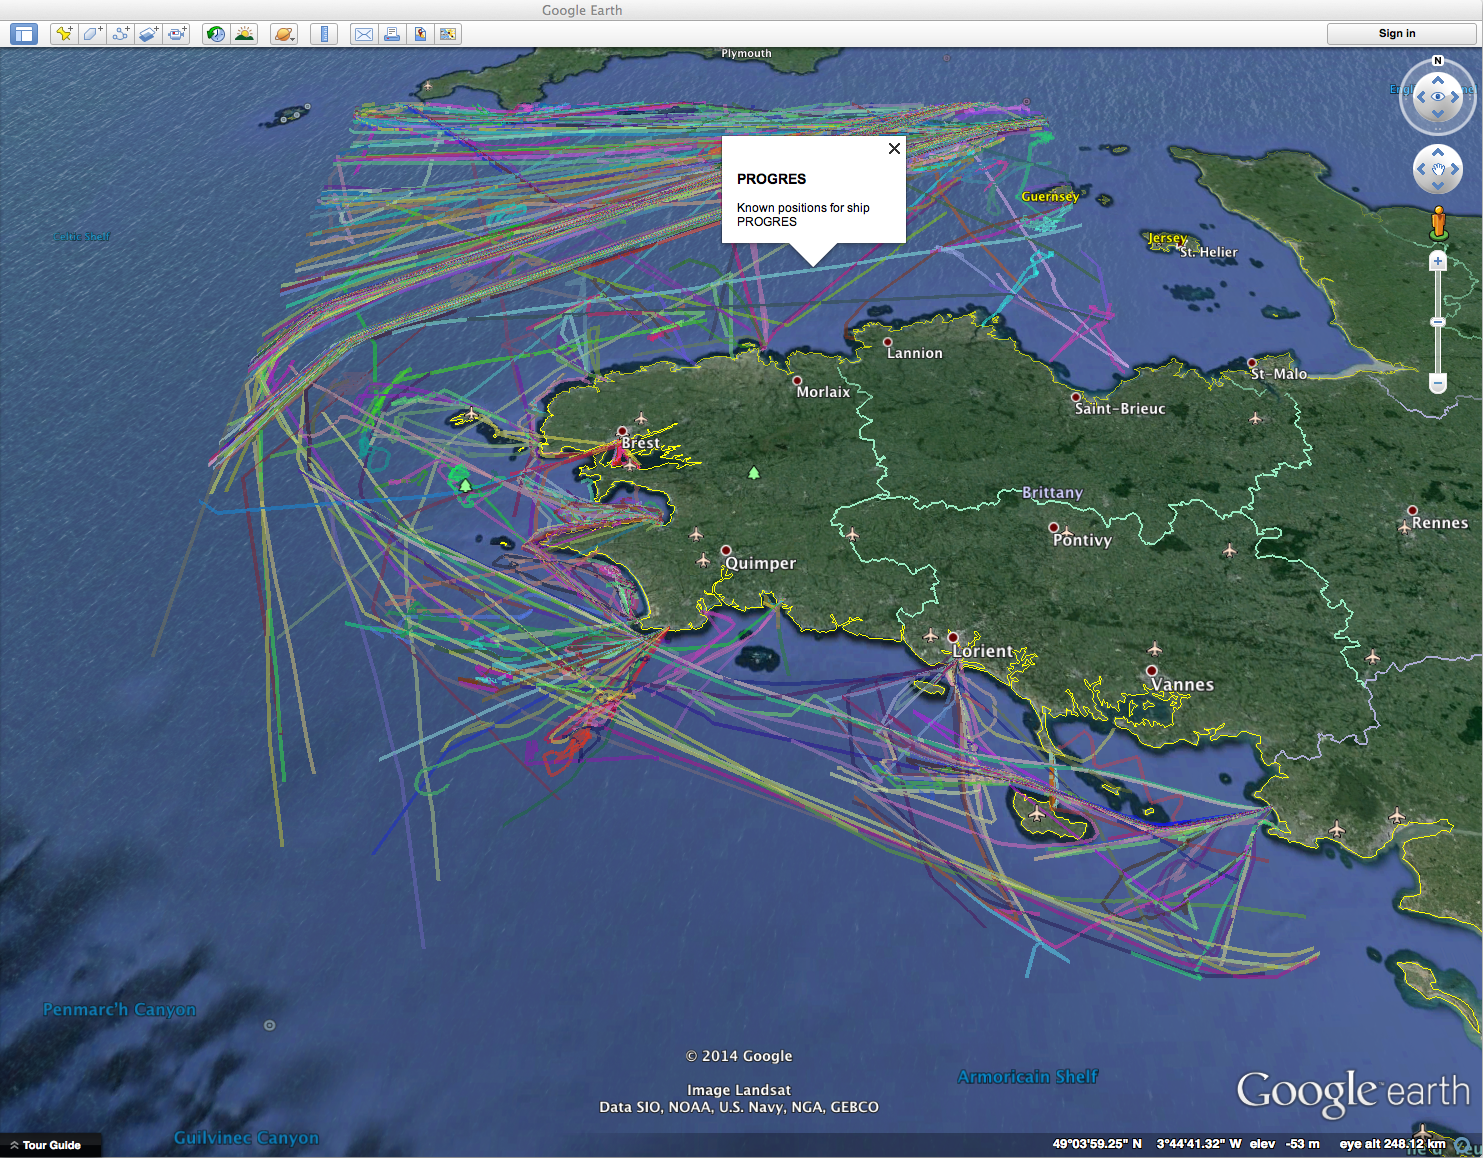
\includegraphics{medias/ships-in-earth.png}

    \hypertarget{choix-dimpluxe9mentation}{%
\subparagraph{Choix d'implémentation\\\\}\label{choix-dimpluxe9mentation}}

    En particulier, dans cet exercice nous allons voir comment on peut gérer
des données sous forme d'instances de classes plutôt que de types de
base. Cela résonne avec la discussion commencée en Semaine 3, Séquence
``Les dictionnaires'', dans le complément ``record-et-dictionnaire''.\\

Dans les exercices de cette semaine-là nous avions uniquement utilisé
des types ``standard'' comme listes, tuples et dictionnaires pour
modéliser les données, cette semaine nous allons faire le choix inverse
et utiliser plus souvent des (instances de) classes.

    \hypertarget{principe-de-lexercice}{%
\subparagraph{Principe de l'exercice\\\\}\label{principe-de-lexercice}}

    On a écrit une application complète, constituée de 4 modules~; on vous
donne le code de trois de ces modules et vous devez écrire le module
manquant.

    \hypertarget{correction}{%
\subparagraph{Correction\\\\}\label{correction}}

    Tout d'abord nous fournissons un jeu de données d'entrées. De plus,
l'application vient avec son propre système de vérification, qui est
très rustique. Il consiste à comparer, une fois les sorties produites,
leur contenu avec les sorties de référence, qui ont été obtenues avec
notre version de l'application.\\

Du coup, le fait de disposer de Google Earth sur votre ordinateur n'est
pas strictement nécessaire, on ne s'en sert pas à proprement parler pour
l'exercice.

\newpage
    \hypertarget{mise-en-place}{%
\subsubsection{Mise en place}\label{mise-en-place}}

    \hypertarget{partez-dun-ruxe9pertoire-vierge}{%
\subparagraph{Partez d'un répertoire
vierge\\\\}\label{partez-dun-ruxe9pertoire-vierge}}

    Pour commencer, créez-vous un répertoire pour travailler à cet exercice.

    \hypertarget{les-donnuxe9es}{%
\subparagraph{Les données\\\\}\label{les-donnuxe9es}}

    Commencez par y installer les données que nous publions dans les formats
suivants~:

\begin{itemize}
\tightlist
\item
  au format \href{data/ships-json.tar}{tar}
\item
  au format \href{data/ships-json.tgz}{tar compressé}
\item
  au format \href{data/ships-json.zip}{zip}
\end{itemize}

Une fois installées, ces données doivent se trouver dans un
sous-répertoire \texttt{json/} qui contient 133 fichiers
\texttt{*.json}~:

\begin{itemize}
\tightlist
\item
  \texttt{json/2013-10-01-00-00-\/-t=10-\/-ext.json}
\item
  \texttt{...}
\item
  \texttt{json/2013-10-01-23-50-\/-t=10.json}
\end{itemize}

    Comme vous pouvez le deviner, il s'agit de données sur le mouvement des
bateaux dans la zone en date du 10 Octobre 2013~; et comme vous le
devinez également, on a quelques exemplaires de données étendues, mais
dans la plupart des cas il s'agit de données abrégées.

    \hypertarget{les-ruxe9sultats-de-ruxe9fuxe9rence}{%
\subparagraph{Les résultats de
référence\\\\}\label{les-ruxe9sultats-de-ruxe9fuxe9rence}}

    De même il vous faut installer les résultats de référence que vous
trouvez ici~:

\begin{itemize}
\tightlist
\item
  au format \href{data/ships-ref.tar}{tar}
\item
  au format \href{data/ships-ref.tgz}{tar compressé (tgz)}
\item
  au format \href{data/ships-ref.zip}{zip}
\end{itemize}

Quel que soit le format choisi, une fois installé ceci doit vous donner
trois fichiers~:

\begin{itemize}
\tightlist
\item
  \texttt{ALL\_SHIPS.kml.ref}
\item
  \texttt{ALL\_SHIPS.txt.ref}
\item
  \texttt{ALL\_SHIPS-v.txt.ref}
\end{itemize}

    \hypertarget{le-code}{%
\subparagraph{Le code\\\\}\label{le-code}}

    Vous pouvez à présent aller chercher les 3 modules suivants~:

\begin{itemize}
\tightlist
\item
  \href{data/merger.py}{\texttt{merger.py}}
\item
  \href{data/compare.py}{\texttt{compare.py}}
\item
  \href{data/kml.py}{\texttt{kml.py}}
\end{itemize}

et les sauver dans le même répertoire.\\

Vous remarquerez que le code est cette fois entièrement rédigé en
anglais, ce que nous vous conseillons de faire aussi souvent que
possible.\\

Votre but dans cet exercice est d'écrire le module manquant
\texttt{shipdict.py} qui permettra à l'application de fonctionner comme
attendu.


    \hypertarget{fonctionnement-de-lapplication}{%
\subsubsection{Fonctionnement de
l'application}\label{fonctionnement-de-lapplication}}

    \hypertarget{comment-est-structuruxe9e-lapplication}{%
\subparagraph{Comment est structurée
l'application\\\\}\label{comment-est-structuruxe9e-lapplication}}

    Le point d'entrée s'appelle \texttt{merger.py}

Il utilise trois modules annexes, qui sont~:

\begin{itemize}
\tightlist
\item
  \texttt{shipdict.py}, qui implémente les classes

  \begin{itemize}
  \tightlist
  \item
    \texttt{Position} qui contient une latitude, une longitude, et un
    timestamp
  \item
    \texttt{Ship} qui modélise un bateau à partir de son \texttt{id} et
    optionnellement \texttt{name} et \texttt{country}
  \item
    \texttt{ShipDict}, qui maintient un index des bateaux
    (essentiellement un dictionnaire)
  \end{itemize}
\item
  \texttt{compare.py} qui implémente

  \begin{itemize}
  \tightlist
  \item
    la classe \texttt{Compare} qui se charge de comparer les fichiers
    résultat avec leur version de référence
  \end{itemize}
\item
  \texttt{kml.py} qui implémente

  \begin{itemize}
  \tightlist
  \item
    la classe \texttt{KML} dans laquelle sont concentrées les fonctions
    liées à la génération de KML~; c'est notamment en fonction de nos
    objectifs pédagogiques que ce choix a été fait.
  \end{itemize}
\end{itemize}

    \hypertarget{lancement}{%
\subparagraph{Lancement\\\\}\label{lancement}}

    Lorsque le programme est complet et qu'il fonctionne correctement, on le
lance comme ceci~:

\begin{verbatim}
    $ python3 merger.py json/*
Opening ALL_SHIPS.txt for listing all named ships
Opening ALL_SHIPS.kml for ship ALL_SHIPS
Comparing ALL_SHIPS.txt and ALL_SHIPS.txt.ref -> OK
Comparing ALL_SHIPS.kml and ALL_SHIPS.kml.ref -> OK
\end{verbatim}

qui comme on le voit produit~:

\begin{itemize}
\tightlist
\item
  \texttt{ALL\_SHIPS.txt} qui résume, par ordre alphabétique les bateaux
  qu'on a trouvés et le nombre de positions pour chacun, et
\item
  \texttt{ALL\_SHIPS.kml} qui est le fichier au format \texttt{KML} qui
  contient toutes les trajectoires.
\end{itemize}

    \hypertarget{mode-bavard-verbose}{%
\subparagraph{Mode bavard (verbose)\\\\}\label{mode-bavard-verbose}}

    On peut également lancer l'application avec l'option
\texttt{-\/-verbose} ou simplement \texttt{-v} sur la ligne de commande,
ce qui donne un résultat plus détaillé. Le code KML généré reste
inchangé, mais la sortie sur le terminal et le fichier de résumé sont
plus étoffés~:

\begin{verbatim}
$ python merger.py --verbose json/*.json
Opening json/2013-10-01-00-00--t=10--ext.json for parsing JSON
Opening json/2013-10-01-00-10--t=10.json for parsing JSON
...
Opening json/2013-10-01-23-40--t=10.json for parsing JSON
Opening json/2013-10-01-23-50--t=10.json for parsing JSON
Opening ALL_SHIPS-v.txt for listing all named ships
Opening ALL_SHIPS.kml for ship ALL_SHIPS
Comparing ALL_SHIPS-v.txt and ALL_SHIPS-v.txt.ref -> OK
Comparing ALL_SHIPS.kml and ALL_SHIPS.kml.ref -> OK
\end{verbatim}

À noter que dans le mode bavard toutes les positions sont listées dans
le résumé au format texte, ce qui le rend beaucoup plus bavard comme
vous pouvez le voir en inspectant la taille des deux fichiers de
référence~:

\begin{verbatim}
$ ls -l ALL_SHIPS*txt.ref v2.0
-rw-r--r--  1 parmentelat  staff  1438681 Dec  4 16:20 ALL_SHIPS-v.txt.ref
-rw-r--r--  1 parmentelat  staff    15331 Dec  4 16:20 ALL_SHIPS.txt.ref
-rw-r--r--  1 parmentelat  staff        0 Dec  4 16:21 v2.0
\end{verbatim}

    \hypertarget{merger.py---help}{%
\subparagraph{\texorpdfstring{\texttt{merger.py\ -\/-help}}{merger.py -\/-help}}\label{merger.py---help}}

    \begin{verbatim}
$ merger.py --help
usage: merger.py [-h] [-v] [-s SHIP_NAME] [-z] [inputs [inputs ...]]

positional arguments:
  inputs

optional arguments:
  -h, --help            show this help message and exit
  -v, --verbose         Verbose mode
  -s SHIP_NAME, --ship SHIP_NAME
                        Restrict to ships by that name
  -z, --gzip            Store kml output in gzip (KMZ) format
\end{verbatim}

    \hypertarget{un-mot-sur-les-donnuxe9es}{%
\subparagraph{Un mot sur les données\\\\}\label{un-mot-sur-les-donnuxe9es}}

    \textbf{Attention}, le contenu détaillé des champs \texttt{extended} et
\texttt{abbreviated} peut être légèrement différent de ce qu'on avait
pour les exercices de la semaine 3, dans lesquels certaines
simplifications ont été apportées.\\

Voici ce avec quoi on travaille cette fois-ci~:

\begin{verbatim}
>>> extended[0]
[228317000, 48.76829, -4.334262, 75, 333, u'2013-09-30T21:54:00', u'MA GONDOLE',
30, 0, u'FGSA', u'FR', u'', u'', u'', u'CLASS B', u'', 13, 3, 0, u'', u'', u'']
\end{verbatim}

c'est-à-dire~:

\begin{verbatim}
[ id, latitude, longitude, _, _, timestamp, name, _, _, _, country, ...]
\end{verbatim}

et en ce qui concerne les données abrégées~:

\begin{verbatim}
>>> abbreviated[0]
[232005670, 49.39331, -5.939922, 33, 269, 3, u'2013-10-01T06:08:00']
\end{verbatim}

c'est-à-dire~:

\begin{verbatim}
[ id, latitude, longitude, _, _, _, timestamp]
\end{verbatim}

    Il y a unicité des \texttt{id} bien entendu (deux relevés qui portent le
même \texttt{id} concernent le même bateau).\\

\textbf{Note historique} Dans une première version de cet exercice, on
avait laissé des doublons, c'est-à-dire des bateaux différents mais de
même nom. Afin de rendre l'exercice plus facile à corriger (notamment
parce que la comparaison des résultats repose sur l'ordre alphabétique),
dans la présente version ces doublons ont été enlevés. Sachez toutefois
que cette unicité est artificielle, aussi efforcez-vous de ne pas écrire
de code qui reposerait sur cette hypothèse.


    \hypertarget{niveaux-pour-lexercice}{%
\subsection{Niveaux pour l'exercice}\label{niveaux-pour-lexercice}}

    Quel que soit le niveau auquel vous choisissez de faire l'exercice, nous
vous conseillons de commencer par lire intégralement les 3 modules qui
sont à votre disposition, dans l'ordre~:

\begin{itemize}
\tightlist
\item
  \texttt{merger.py} qui est le chef d'orchestre de toute cette
  affaire~;
\item
  \texttt{compare.py} qui est très simple~;
\item
  \texttt{kml.py} qui ne présente pas grand intérêt en soi si ce n'est
  pour l'utilisation de
  \href{https://docs.python.org/3/library/string.html\#template-strings}{la
  classe \texttt{string.Template}} qui peut être utile dans d'autres
  contextes également.
\end{itemize}


    En \textbf{niveau avancé}, l'énoncé pourrait s'arrêter là~; vous lisez
le code qui est fourni et vous en déduisez ce qui manque pour faire
fonctionner le tout. En cas de difficulté liée aux arrondis avec le mode
bavard, vous pouvez toutefois vous inspirer du code qui est donné dans
la toute dernière section de cet énoncé (section ``Un dernier indice''),
pour traduire un flottant en représentation textuelle.\\

    Vous pouvez considérer que vous avez achevé l'exercice lorsque les deux
appels suivants affichent les deux dernières lignes avec OK~:

\begin{verbatim}
$ python merger.py json/*.json
...
Comparing ALL_SHIPS.txt and ALL_SHIPS.txt.ref -> OK
Comparing ALL_SHIPS.kml and ALL_SHIPS.kml.ref -> OK



$ python merger.py -v json/*.json
...
Comparing ALL_SHIPS-v.txt and ALL_SHIPS-v.txt.ref -> OK
Comparing ALL_SHIPS.kml and ALL_SHIPS.kml.ref -> OK
\end{verbatim}

    Le cas où on lance \texttt{merger.py} avec l'option bavarde est
facultatif.



    En \textbf{niveau intermédiaire}, nous vous donnons ci-dessous un
extrait de ce que donne \texttt{help} sur les classes manquantes de
manière à vous donner une indication de ce que vous devez écrire.

    \hypertarget{classe-position}{%
\subparagraph{\texorpdfstring{Classe
\texttt{Position}}{Classe Position}}\label{classe-position}}

    \begin{verbatim}
Help on class Position in module shipdict:

class Position(__builtin__.object)
 |  a position atom with timestamp attached
 |  
 |  Methods defined here:
 |  
 |  __init__(self, latitude, longitude, timestamp)
 |      constructor
 |  
 |  __repr__(self)
 |      only used when merger.py is run in verbose mode
 |  
\end{verbatim}

    \textbf{Notes}

\begin{itemize}
\tightlist
\item
  certaines autres classes comme \texttt{KML} sont également
  susceptibles d'accéder aux champs internes d'une instance de la classe
  \texttt{Position} en faisant simplement \texttt{position.latitude}
\item
  La classe \texttt{Position} redéfinit \texttt{\_\_repr\_\_}, ceci est
  utilisé uniquement dans la sortie en mode bavard.
\end{itemize}

    \hypertarget{classe-ship}{%
\subparagraph{\texorpdfstring{Classe
\texttt{Ship}}{Classe Ship}}\label{classe-ship}}

    \begin{verbatim}
Help on class Ship in module shipdict:

class Ship(__builtin__.object)
 |  a ship object, that requires a ship id, 
 |  and optionally a ship name and country
 |  which can also be set later on
 |  
 |  this object also manages a list of known positions
 |  
 |  Methods defined here:
 |  
 |  __init__(self, id, name=None, country=None)
 |      constructor
 |  
 |  add_position(self, position)
 |      insert a position relating to this ship
 |      positions are not kept in order so you need 
 |      to call `sort_positions` once you're done
 |  
 |  sort_positions(self)
 |      sort list of positions by chronological order
\end{verbatim}

    \hypertarget{classe-shipdict}{%
\subparagraph{\texorpdfstring{Classe
\texttt{Shipdict}}{Classe Shipdict}}\label{classe-shipdict}}

    \begin{verbatim}
Help on class ShipDict in module shipdict:

class ShipDict(__builtin__.dict)
 |  a repository for storing all ships that we know about
 |  indexed by their id
 |  
 |  Method resolution order:
 |      ShipDict
 |      __builtin__.dict
 |      __builtin__.object
 |  
 |  Methods defined here:
 |  
 |  __init__(self)
 |      constructor
 |  
 |  __repr__(self)
 |  
 |  add_abbreviated(self, chunk)
 |      adds an abbreviated data chunk to the repository
 |  
 |  add_chunk(self, chunk)
 |      chunk is a plain list coming from the JSON data
 |      and be either extended or abbreviated
 |      
 |      based on the result of is_abbreviated(), 
 |      gets sent to add_extended or add_abbreviated
 |  
 |  add_extended(self, chunk)
 |      adds an extended data chunk to the repository
 |  
 |  all_ships(self)
 |      returns a list of all ships known to us
 |  
 |  clean_unnamed(self)
 |      Because we enter abbreviated and extended data
 |      in no particular order, and for any time period,
 |      we might have ship instances with no name attached
 |      This method removes such entries from the dict
 |  
 |  is_abbreviated(self, chunk)
 |      depending on the size of the incoming data chunk, 
 |      guess if it is an abbreviated or extended data
 |  
 |  ships_by_name(self, name)
 |      returns a list of all known ships with name <name>
 |  
 |  sort(self)
 |      makes sure all the ships have their positions
 |      sorted in chronological order
\end{verbatim}

    \hypertarget{un-dernier-indice}{%
\subparagraph{Un dernier indice\\\\}\label{un-dernier-indice}}

    Pour éviter de la confusion, voici le code que nous utilisons pour
transformer un flottant en coordonnées lisibles dans le résumé généré en
mode bavard.

    \begin{verbatim}
def d_m_s(f):
    """
    makes a float readable; e.g. transforms 2.5 into 2.30'00'' 
    we avoid using ° to keep things simple
    input is assumed positive
    """
    d = int (f)
    m = int((f-d)*60)
    s = int( (f-d)*3600 - 60*m)
    return f"{d:02d}.{m:02d}'{s:02d}''"
\end{verbatim}

%    \chapter{L'écosystème data science Python}
	
%	\include{w7-s1-c1-installation}
%	\include{w7-s2-c00-intro-numpy}
%	\include{w7-s2-c01-dimension1}
%	\include{w7-s2-c02-dtype}
%	\include{w7-s2-c03-shape}
%	\include{w7-s2-c04-initialisation}
%	\include{w7-s2-c05-broadcasting}
%	\include{w7-s2-c05-x1-stairs}
%	\include{w7-s2-c06-indexing-slicing}
%	\include{w7-s2-c07-operations-logiques}
%	\include{w7-s2-c08-algebre-lineaire}
%	\include{w7-s2-c09-indexation-evoluee}
%	\include{w7-s2-c10-divers}
%	\include{w7-s3-c01-data-science}
%	\include{w7-s3-c02-Series}
%	\include{w7-s3-c03-DataFrame}
%	\include{w7-s3-c04-operations-avancee-pandas}
%	\include{w7-s4-c01-matplotlib-2d}
%	\include{w7-s4-c02-matplotlib-3d}
%	\include{w7-s4-c04-bokeh-et-al}

%    \chapter{Programmation asynchrone-asyncio}
	
%	    
    
    
    

    

    \hypertarget{essayez-vous-muxeame}{%
\section{Essayez vous-même}\label{essayez-vous-muxeame}}

    \hypertarget{compluxe9ment---niveau-avancuxe9}{%
\subsection{Complément - niveau
avancé}\label{compluxe9ment---niveau-avancuxe9}}

    Pour des raisons techniques, il ne nous est pas possible de mettre en
ligne un notebook qui vous permette de reproduire les exemples de la
vidéo.

    C'est pourquoi, si vous êtes intéressés à reproduire vous-même les
expériences de la vidéo - à savoir, aller chercher plusieurs URLs de
manière séquentielle ou en parallèle - \href{data/async_http.py}{vous
pouvez télécharger le code fourni dans ce lien}.

    Il s'agit d'un simple script, qui reprend les 3 approches de la vidéo~:

\begin{itemize}
\tightlist
\item
  accès en séquence~;
\item
  accès asynchrones avec \texttt{fetch}~;
\item
  accès asynchrones avec \texttt{fetch2} (qui pour rappel provoque un
  tick à chaque ligne qui revient d'un des serveurs web).
\end{itemize}

À part pour l'appel à \texttt{sys.stdout.flush()}, ce code est
rigoureusement identique à celui utilisé dans la vidéo. On doit faire
ici cet appel à \texttt{flush()}, dans le mode avec \texttt{fetch2}, car
sinon les sorties de notre script sont bufferisées, et apparaissent
toutes ensemble à la fin du programme, c'est beaucoup moins drôle.

    Voici son mode d'emploi~:

    \begin{Shaded}
\begin{Highlighting}[frame=lines,framerule=0.6mm,rulecolor=\color{asisframecolor}]
\NormalTok{$ python3 async_http.py }\OperatorTok{--}\BuiltInTok{help}
\NormalTok{usage: async_http.py [}\OperatorTok{-}\NormalTok{h] [}\OperatorTok{-}\NormalTok{s] [}\OperatorTok{-}\NormalTok{d] [urls [urls ...]]}

\NormalTok{positional arguments:}
\NormalTok{  urls              URL}\StringTok{'s to be fetched}

\StringTok{optional arguments:}
\StringTok{  -h, --help        show this help message and exit}
\StringTok{  -s, --sequential  run sequentially}
\StringTok{  -d, --details     show details of lines as they show up (using fetch2)}
\end{Highlighting}
\end{Shaded}

    Et voici les chiffres que j'obtiens lorsque je l'utilise dans une
configuration réseau plus stable que dans la vidéo, on voit ici un réel
gain à l'utilisation de communications asynchrones~(à cause de
conditions réseau un peu erratiques lors de la vidéo, on n'y voit pas
bien le gain obtenu) :

    \begin{Shaded}
\begin{Highlighting}[frame=lines,framerule=0.6mm,rulecolor=\color{asisframecolor}]
\NormalTok{$ python3 async_http.py }\OperatorTok{-}\NormalTok{s}
\NormalTok{Running sequential mode on }\DecValTok{4}\NormalTok{ URLs}
\NormalTok{http:}\OperatorTok{//}\NormalTok{www.irs.gov}\OperatorTok{/}\NormalTok{pub}\OperatorTok{/}\NormalTok{irs}\OperatorTok{-}\NormalTok{pdf}\OperatorTok{/}\NormalTok{f1040.pdf returned }\DecValTok{179940}\NormalTok{ chars}
\NormalTok{http:}\OperatorTok{//}\NormalTok{www.irs.gov}\OperatorTok{/}\NormalTok{pub}\OperatorTok{/}\NormalTok{irs}\OperatorTok{-}\NormalTok{pdf}\OperatorTok{/}\NormalTok{f1040ez.pdf returned }\DecValTok{113242}\NormalTok{ chars}
\NormalTok{http:}\OperatorTok{//}\NormalTok{www.irs.gov}\OperatorTok{/}\NormalTok{pub}\OperatorTok{/}\NormalTok{irs}\OperatorTok{-}\NormalTok{pdf}\OperatorTok{/}\NormalTok{f1040es.pdf returned }\DecValTok{395201}\NormalTok{ chars}
\NormalTok{http:}\OperatorTok{//}\NormalTok{www.irs.gov}\OperatorTok{/}\NormalTok{pub}\OperatorTok{/}\NormalTok{irs}\OperatorTok{-}\NormalTok{pdf}\OperatorTok{/}\NormalTok{f1040sb.pdf returned }\DecValTok{73189}\NormalTok{ chars}
\NormalTok{duration }\OperatorTok{=} \FloatTok{9.80829906463623}\NormalTok{s}
\end{Highlighting}
\end{Shaded}

    \begin{Shaded}
\begin{Highlighting}[frame=lines,framerule=0.6mm,rulecolor=\color{asisframecolor}]
\NormalTok{$ python3 async_http.py}
\NormalTok{Running simple mode (fetch) on }\DecValTok{4}\NormalTok{ URLs}
\NormalTok{fetching http:}\OperatorTok{//}\NormalTok{www.irs.gov}\OperatorTok{/}\NormalTok{pub}\OperatorTok{/}\NormalTok{irs}\OperatorTok{-}\NormalTok{pdf}\OperatorTok{/}\NormalTok{f1040.pdf}
\NormalTok{fetching http:}\OperatorTok{//}\NormalTok{www.irs.gov}\OperatorTok{/}\NormalTok{pub}\OperatorTok{/}\NormalTok{irs}\OperatorTok{-}\NormalTok{pdf}\OperatorTok{/}\NormalTok{f1040sb.pdf}
\NormalTok{fetching http:}\OperatorTok{//}\NormalTok{www.irs.gov}\OperatorTok{/}\NormalTok{pub}\OperatorTok{/}\NormalTok{irs}\OperatorTok{-}\NormalTok{pdf}\OperatorTok{/}\NormalTok{f1040es.pdf}
\NormalTok{fetching http:}\OperatorTok{//}\NormalTok{www.irs.gov}\OperatorTok{/}\NormalTok{pub}\OperatorTok{/}\NormalTok{irs}\OperatorTok{-}\NormalTok{pdf}\OperatorTok{/}\NormalTok{f1040ez.pdf}
\NormalTok{http:}\OperatorTok{//}\NormalTok{www.irs.gov}\OperatorTok{/}\NormalTok{pub}\OperatorTok{/}\NormalTok{irs}\OperatorTok{-}\NormalTok{pdf}\OperatorTok{/}\NormalTok{f1040.pdf response status }\DecValTok{200}
\NormalTok{http:}\OperatorTok{//}\NormalTok{www.irs.gov}\OperatorTok{/}\NormalTok{pub}\OperatorTok{/}\NormalTok{irs}\OperatorTok{-}\NormalTok{pdf}\OperatorTok{/}\NormalTok{f1040ez.pdf response status }\DecValTok{200}
\NormalTok{http:}\OperatorTok{//}\NormalTok{www.irs.gov}\OperatorTok{/}\NormalTok{pub}\OperatorTok{/}\NormalTok{irs}\OperatorTok{-}\NormalTok{pdf}\OperatorTok{/}\NormalTok{f1040sb.pdf response status }\DecValTok{200}
\NormalTok{http:}\OperatorTok{//}\NormalTok{www.irs.gov}\OperatorTok{/}\NormalTok{pub}\OperatorTok{/}\NormalTok{irs}\OperatorTok{-}\NormalTok{pdf}\OperatorTok{/}\NormalTok{f1040es.pdf response status }\DecValTok{200}
\NormalTok{http:}\OperatorTok{//}\NormalTok{www.irs.gov}\OperatorTok{/}\NormalTok{pub}\OperatorTok{/}\NormalTok{irs}\OperatorTok{-}\NormalTok{pdf}\OperatorTok{/}\NormalTok{f1040sb.pdf returned }\DecValTok{75864} \BuiltInTok{bytes}
\NormalTok{http:}\OperatorTok{//}\NormalTok{www.irs.gov}\OperatorTok{/}\NormalTok{pub}\OperatorTok{/}\NormalTok{irs}\OperatorTok{-}\NormalTok{pdf}\OperatorTok{/}\NormalTok{f1040.pdf returned }\DecValTok{186928} \BuiltInTok{bytes}
\NormalTok{http:}\OperatorTok{//}\NormalTok{www.irs.gov}\OperatorTok{/}\NormalTok{pub}\OperatorTok{/}\NormalTok{irs}\OperatorTok{-}\NormalTok{pdf}\OperatorTok{/}\NormalTok{f1040ez.pdf returned }\DecValTok{117807} \BuiltInTok{bytes}
\NormalTok{http:}\OperatorTok{//}\NormalTok{www.irs.gov}\OperatorTok{/}\NormalTok{pub}\OperatorTok{/}\NormalTok{irs}\OperatorTok{-}\NormalTok{pdf}\OperatorTok{/}\NormalTok{f1040es.pdf returned }\DecValTok{409193} \BuiltInTok{bytes}
\NormalTok{duration }\OperatorTok{=} \FloatTok{2.211031913757324}\NormalTok{s}
\end{Highlighting}
\end{Shaded}

    N'hésitez pas à utiliser ceci comme base pour expérimenter.

Nous verrons en fin de semaine un autre exemple qui cette fois
illustrera l'interaction avec les sous-processus.


    % Add a bibliography block to the postdoc
    
    
    

%	    
    
    
    

    

    \hypertarget{asyncio---un-exemple-un-peu-plus-ruxe9aliste}{%
\section{\texorpdfstring{\texttt{asyncio} - un exemple un peu plus
réaliste}{asyncio - un exemple un peu plus réaliste}}\label{asyncio---un-exemple-un-peu-plus-ruxe9aliste}}

    \hypertarget{compluxe9ment---niveau-avancuxe9}{%
\subsection{Complément - niveau
avancé}\label{compluxe9ment---niveau-avancuxe9}}

    Pour des raisons techniques, il n'est pas possible de mettre en ligne un
notebook pour les activités liées au réseau, qui sont pourtant
clairement dans le coeur de cible de la bibliothèque - souvenez-vous que
ce paradigme de programmation a été développé au départ par les projets
comme tornado, qui se préoccupe de services Web.

    Aussi, pour illustrer les possibilités offertes par \texttt{asyncio} sur
un exemple un peu plus significatif que ceux qui utilisent
\texttt{asyncio.sleep}, nous allons écrire le début d'une petite
architecture de jeu.

Il s'agit pour nous principalement d'illustrer les capacités de
\texttt{asyncio} en matière de gestion de sous-processus, car c'est
quelque chose que l'on peut déployer dans le contexte des notebooks.

    Nous allons procéder en deux temps. Dans ce premier notebook nous allons
écrire un petit programme Python qui s'appelle \texttt{players.py}.
C'est une brique de base dans notre architecture, dans le second
notebook on écrira un programme qui lance (sous la forme de
sous-processus) plusieurs instances de \texttt{players.py}.

    \hypertarget{le-programme-players.py}{%
\subsubsection{\texorpdfstring{Le programme
\texttt{players.py}}{Le programme players.py}}\label{le-programme-players.py}}

    Mais dans l'immédiat, voyons ce que fait \texttt{players.py}. On veut
modéliser le comportement de plusieurs joueurs.

Chaque joueur a un comportement hyper basique, il émet simplement à des
intervalles aléatoires un événement du type~:

\begin{quote}
je suis le joueur John et je vais dans la direction Nord
\end{quote}

Chaque joueur a un nom, et une fréquence moyenne, et un nombre de
cycles.

Par ailleurs pour être un peu vraisemblable, il y a quatre directions
\texttt{N}, \texttt{S}, \texttt{E} et \texttt{W}, mais que l'on
n'utilisera pas vraiment dans la suite.

    Voyez ici le code de \texttt{players.py}

    Comme vous le voyez, dans ce premier exemple nous n'utilisons à nouveau
que \texttt{asyncio.sleep} pour modéliser chaque joueur, dont la logique
peut être illustrée simplement comme ceci (où la ligne horizontale
représente le temps)~:

    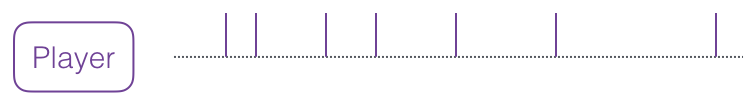
\includegraphics{media/player.png}

    Pour éviter de nous noyer dans des configurations compliquées, on a
embarqué dans \texttt{players} plusieurs configurations prédéfinies,
mais dans tous les cas chacune de ces configurations crée deux joueurs.

    La logique des deux joueurs est simplement juxtaposée, ou si on préfère
superposée, par \texttt{asyncio.gather}, ce qui fait que la sortie de
\texttt{players.py} ressemble à ceci~:

    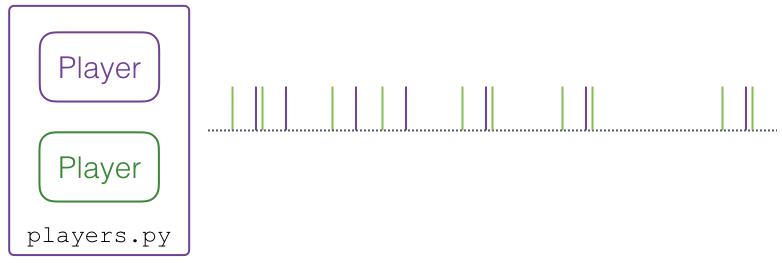
\includegraphics{media/players.png}

    \begin{Verbatim}[commandchars=\\\{\},frame=single,framerule=0.3mm,rulecolor=\color{cellframecolor}]
{\color{incolor}In [{\color{incolor}1}]:} \PY{c+c1}{\PYZsh{} je peux lancer un sous\PYZhy{}processus}
        \PY{c+c1}{\PYZsh{} depuis le notebook}
        \PY{o}{!}data/players.py
\end{Verbatim}


    \begin{Verbatim}[commandchars=\\\{\},frame=single,framerule=0.3mm,rulecolor=\color{cellframecolor}]
N john
S mary
W john
W mary
S mary
S mary
S john
N mary
E john
E mary
W mary
W mary
\end{Verbatim}

    \begin{Verbatim}[commandchars=\\\{\},frame=single,framerule=0.3mm,rulecolor=\color{cellframecolor}]
{\color{incolor}In [{\color{incolor}2}]:} \PY{c+c1}{\PYZsh{} ou une autre configuration}
        \PY{o}{!}data/players.py \PY{l+m}{2}
\end{Verbatim}


    \begin{Verbatim}[commandchars=\\\{\},frame=single,framerule=0.3mm,rulecolor=\color{cellframecolor}]
W bill
W jane
N jane
N bill
W jane
N bill
S bill
S bill
W jane
W bill
W jane
\end{Verbatim}

    Nous allons voir dans le notebook suivant comment on peut orchestrer
plusieurs instances du programme \texttt{players.py}, et prolonger cette
logique de juxtaposition / mélange des sorties, mais cette fois au
niveau de plusieurs processus.


    % Add a bibliography block to the postdoc
    
    
    

%	    
    
    
    

    

    \hypertarget{gestion-de-sous-process}{%
\section{Gestion de sous-process}\label{gestion-de-sous-process}}

    \hypertarget{compluxe9ment---niveau-truxe8s-avancuxe9}{%
\subsection{Complément - niveau (très)
avancé}\label{compluxe9ment---niveau-truxe8s-avancuxe9}}

    Dans ce second notebook, nous allons étudier un deuxième programme
Python, que j'appelle \texttt{game.py} (en fait c'est le présent
notebook).

    \hypertarget{fonctions-de-game.py}{%
\subsubsection{\texorpdfstring{Fonctions de
\texttt{game.py}}{Fonctions de game.py}}\label{fonctions-de-game.py}}

    Son travail va consister à faire plusieurs choses en même temps~; pour
rester le plus simple possible, on va se contenter des trois fonctions
suivantes~:

\begin{itemize}
\tightlist
\item
  \emph{scheduler} (chef d'orchestre)~: on veut lancer à des moments
  préprogrammés des instances (sous-process) de \texttt{players.py}~;
\item
  \emph{multiplexer} (agrégateur)~: on veut lire et imprimer au fur et à
  mesure les messages émis par les sous-processus~;
\item
  horloge~: on veut également afficher chaque seconde le temps écoulé
  depuis le début.
\end{itemize}

    En pratique, le programme \texttt{game.py} serait plutôt le serveur du
jeu qui reçoit les mouvements de tous les joueurs, et diffuse ensuite en
retour, en mode broadcast, un état du jeu à tous les participants.

    Mais dans notre version hyper simpliste, ça donne un comportement que
j'ai essayé d'illustrer comme ceci~:

    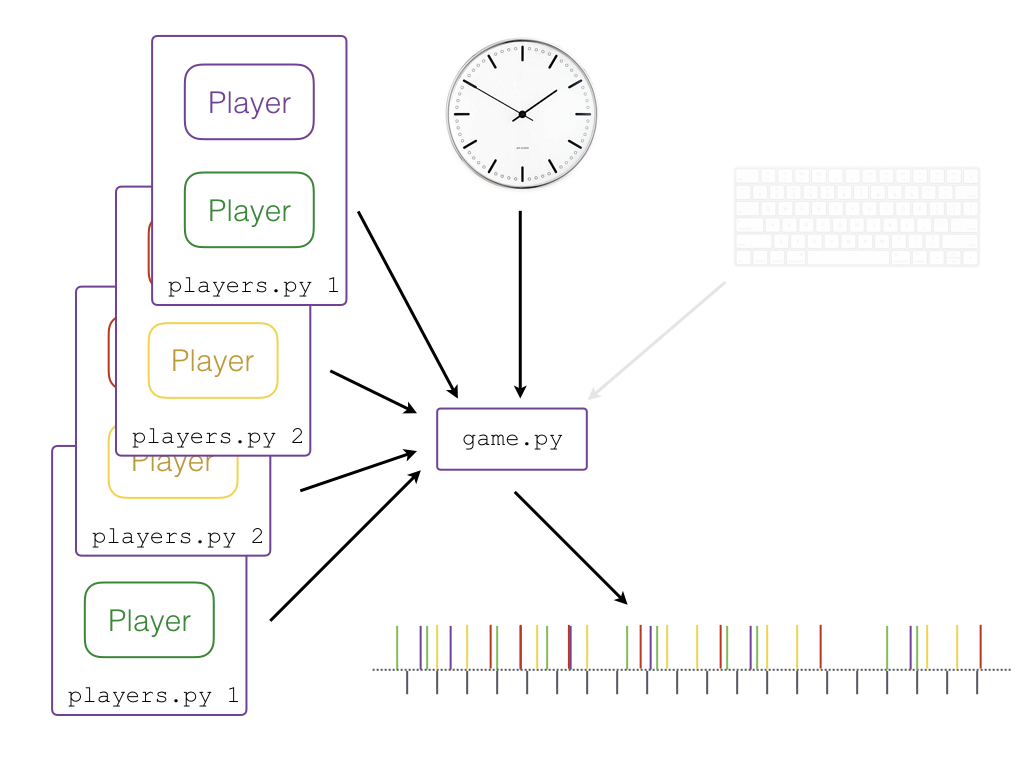
\includegraphics{media/game.png}

    \hypertarget{remarque-concernant-les-notebooks-et-le-clavier}{%
\subparagraph{Remarque concernant les notebooks et le
clavier}\label{remarque-concernant-les-notebooks-et-le-clavier}}

    Lorsqu'on exécute du code Python dans un notebook, les entrées clavier
sont en fait interceptées par le navigateur Web~; du coup on ne peut pas
facilement (du tout~?) faire tourner dans un notebook un programme
asynchrone qui réagirait aussi aux événements de type entrée clavier.

C'est pour cette raison que le clavier apparaît sur ma figure en
filigrane. Si vous allez jusqu'à exécuter ce notebook localement sur
votre machine (voir plus bas), vous pourrez utiliser le clavier pour
ajouter à la volée des éléments dans le scénario - en entrant des
numéros de 1 à 4 au moment voulu.

    \hypertarget{terminaison}{%
\subparagraph{Terminaison}\label{terminaison}}

    Pour rester simple et en l'absence de clavier, j'ai choisi de terminer
le programme lorsque le dernier sous-processus se termine.

    \hypertarget{le-programme-game.py}{%
\subsubsection{\texorpdfstring{Le programme
\texttt{game.py}}{Le programme game.py}}\label{le-programme-game.py}}

    C'est ce notebook qui va jouer pour nous le rôle du programme
\texttt{game.py}.

    \begin{Verbatim}[commandchars=\\\{\},frame=single,framerule=0.3mm,rulecolor=\color{cellframecolor}]
{\color{incolor}In [{\color{incolor}1}]:} \PY{k+kn}{import} \PY{n+nn}{asyncio}
        \PY{k+kn}{import} \PY{n+nn}{sys}
\end{Verbatim}


    \begin{Verbatim}[commandchars=\\\{\},frame=single,framerule=0.3mm,rulecolor=\color{cellframecolor}]
{\color{incolor}In [{\color{incolor}2}]:} \PY{c+c1}{\PYZsh{} cette constante est utile pour déclarer qu\PYZsq{}on a l\PYZsq{}intention}
        \PY{c+c1}{\PYZsh{} de lire les sorties (stout et stderr)}
        \PY{c+c1}{\PYZsh{} de nos sous\PYZhy{}process par l\PYZsq{}intermédiaire de pipes}
        \PY{k+kn}{from} \PY{n+nn}{subprocess} \PY{k}{import} \PY{n}{PIPE}
\end{Verbatim}


    Commençons par la classe \texttt{Scheduler}~; c'est celle qui va se
charger de lancer les sous-process selon un scénario. Pour ne pas se
compliquer la vie on choisit de représenter un scénario (un script)
comme une liste de tuples de la forme~:

\begin{Shaded}
\begin{Highlighting}[frame=lines,framerule=0.6mm,rulecolor=\color{asisframecolor}]
\NormalTok{script }\OperatorTok{=}\NormalTok{ [ (secondes, predef), ...]}
\end{Highlighting}
\end{Shaded}

qui signifie de lancer, un délai de \texttt{secondes} secondes après le
début du programme, le programme \texttt{players.py} dans la
configuration \texttt{predef} - de 1 à 4 donc.

    \begin{Verbatim}[commandchars=\\\{\},frame=single,framerule=0.3mm,rulecolor=\color{cellframecolor}]
{\color{incolor}In [{\color{incolor}3}]:} \PY{k}{class} \PY{n+nc}{Scheduler}\PY{p}{:}
        
            \PY{k}{def} \PY{n+nf}{\PYZus{}\PYZus{}init\PYZus{}\PYZus{}}\PY{p}{(}\PY{n+nb+bp}{self}\PY{p}{,} \PY{n}{script}\PY{p}{)}\PY{p}{:}
        
                \PY{c+c1}{\PYZsh{} on trie le script par ordre chronologique}
                \PY{n+nb+bp}{self}\PY{o}{.}\PY{n}{script} \PY{o}{=} \PY{n+nb}{list}\PY{p}{(}\PY{n}{script}\PY{p}{)}
                \PY{n+nb+bp}{self}\PY{o}{.}\PY{n}{script}\PY{o}{.}\PY{n}{sort}\PY{p}{(}\PY{n}{key} \PY{o}{=} \PY{k}{lambda} \PY{n}{time\PYZus{}predef} \PY{p}{:} \PY{n}{time\PYZus{}predef}\PY{p}{[}\PY{l+m+mi}{0}\PY{p}{]}\PY{p}{)}
        
                \PY{c+c1}{\PYZsh{} juste pour donner un numéro à chaque processus}
                \PY{n+nb+bp}{self}\PY{o}{.}\PY{n}{counter} \PY{o}{=} \PY{l+m+mi}{1}
                \PY{c+c1}{\PYZsh{} combien de processus sont actifs}
                \PY{n+nb+bp}{self}\PY{o}{.}\PY{n}{running} \PY{o}{=} \PY{l+m+mi}{0}
        
            \PY{k}{async} \PY{k}{def} \PY{n+nf}{run}\PY{p}{(}\PY{n+nb+bp}{self}\PY{p}{)}\PY{p}{:}
                \PY{l+s+sd}{\PYZdq{}\PYZdq{}\PYZdq{}}
        \PY{l+s+sd}{        fait tout le travail, c\PYZsq{}est\PYZhy{}à\PYZhy{}dire :}
        \PY{l+s+sd}{        * lance tous les sous\PYZhy{}processus à l\PYZsq{}heure indiquée}
        \PY{l+s+sd}{        * et aussi en préambule, pour le mode avec clavier,}
        \PY{l+s+sd}{          arme une callback sur l\PYZsq{}entrée standard}
        \PY{l+s+sd}{        \PYZdq{}\PYZdq{}\PYZdq{}}
                \PY{c+c1}{\PYZsh{} pour le mode avec clavier (pas fonctionnel dans le notebook)}
                \PY{c+c1}{\PYZsh{} on arme une callback sur stdin}
                \PY{n}{asyncio}\PY{o}{.}\PY{n}{get\PYZus{}event\PYZus{}loop}\PY{p}{(}\PY{p}{)}\PY{o}{.}\PY{n}{add\PYZus{}reader}\PY{p}{(}
                    \PY{c+c1}{\PYZsh{} il nous faut un file descriptor, pas un objet Python}
                    \PY{n}{sys}\PY{o}{.}\PY{n}{stdin}\PY{o}{.}\PY{n}{fileno}\PY{p}{(}\PY{p}{)}\PY{p}{,}
                    \PY{c+c1}{\PYZsh{} la callback}
                    \PY{n}{Scheduler}\PY{o}{.}\PY{n}{read\PYZus{}keyboard\PYZus{}line}\PY{p}{,}
                    \PY{c+c1}{\PYZsh{} les arguments de la callback}
                    \PY{c+c1}{\PYZsh{} cette fois c\PYZsq{}est un objet Python}
                    \PY{n+nb+bp}{self}\PY{p}{,} \PY{n}{sys}\PY{o}{.}\PY{n}{stdin}
                \PY{p}{)}
                \PY{c+c1}{\PYZsh{} le scénario prédéfini}
                \PY{n}{epoch} \PY{o}{=} \PY{l+m+mi}{0}
                \PY{k}{for} \PY{n}{tick}\PY{p}{,} \PY{n}{predef} \PY{o+ow}{in} \PY{n+nb+bp}{self}\PY{o}{.}\PY{n}{script}\PY{p}{:}
                    \PY{c+c1}{\PYZsh{} attendre le bon moment}
                    \PY{k}{await} \PY{n}{asyncio}\PY{o}{.}\PY{n}{sleep}\PY{p}{(}\PY{n}{tick} \PY{o}{\PYZhy{}} \PY{n}{epoch}\PY{p}{)}
                    \PY{c+c1}{\PYZsh{} pour le prochain}
                    \PY{n}{epoch} \PY{o}{=} \PY{n}{tick}
                    \PY{n}{asyncio}\PY{o}{.}\PY{n}{ensure\PYZus{}future}\PY{p}{(}\PY{n+nb+bp}{self}\PY{o}{.}\PY{n}{fork\PYZus{}players}\PY{p}{(}\PY{n}{predef}\PY{p}{)}\PY{p}{)}
        
            \PY{k}{async} \PY{k}{def} \PY{n+nf}{fork\PYZus{}players}\PY{p}{(}\PY{n+nb+bp}{self}\PY{p}{,} \PY{n}{predef}\PY{p}{)}\PY{p}{:}
                \PY{l+s+sd}{\PYZdq{}\PYZdq{}\PYZdq{}}
        \PY{l+s+sd}{        lance maintenant une instance de players avec cette config}
        
        \PY{l+s+sd}{        puis}
        \PY{l+s+sd}{        écoute à la fois sdtout et stderr, et les imprime}
        \PY{l+s+sd}{        (bon c\PYZsq{}est vrai que players n\PYZsq{}écrit rien sur stderr)}
        \PY{l+s+sd}{        attend la fin du sous\PYZhy{}processus (avec wait())}
        \PY{l+s+sd}{        et retourne son code de retour (exitcode) du sous\PYZhy{}processus}
        
        \PY{l+s+sd}{        par commodité on décide d\PYZsq{}arrêter la boucle principale}
        \PY{l+s+sd}{        lorsqu\PYZsq{}il n\PYZsq{}y a plus aucun process actif}
        \PY{l+s+sd}{        \PYZdq{}\PYZdq{}\PYZdq{}}
        
                \PY{c+c1}{\PYZsh{} la commande à lancer pour forker une instance de players.py}
                \PY{n}{command} \PY{o}{=} \PY{n}{f}\PY{l+s+s2}{\PYZdq{}}\PY{l+s+s2}{python3 \PYZhy{}u data/players.py }\PY{l+s+si}{\PYZob{}predef\PYZcb{}}\PY{l+s+s2}{\PYZdq{}}\PY{o}{.}\PY{n}{split}\PY{p}{(}\PY{p}{)}
                \PY{c+c1}{\PYZsh{} pour afficher un nom un peu plus parlant}
                \PY{n}{worker} \PY{o}{=} \PY{n}{f}\PY{l+s+s2}{\PYZdq{}}\PY{l+s+s2}{ps\PYZsh{}}\PY{l+s+si}{\PYZob{}self.counter\PYZcb{}}\PY{l+s+s2}{ (predef }\PY{l+s+si}{\PYZob{}predef\PYZcb{}}\PY{l+s+s2}{)}\PY{l+s+s2}{\PYZdq{}}
                \PY{c+c1}{\PYZsh{} housekeeping}
                \PY{n+nb+bp}{self}\PY{o}{.}\PY{n}{counter} \PY{o}{+}\PY{o}{=} \PY{l+m+mi}{1}
                \PY{n+nb+bp}{self}\PY{o}{.}\PY{n}{running} \PY{o}{+}\PY{o}{=} \PY{l+m+mi}{1}
                \PY{c+c1}{\PYZsh{} c\PYZsq{}est là que ça se passe : on forke}
                \PY{n+nb}{print}\PY{p}{(}\PY{l+m+mi}{8} \PY{o}{*} \PY{l+s+s1}{\PYZsq{}}\PY{l+s+s1}{\PYZgt{}}\PY{l+s+s1}{\PYZsq{}}\PY{p}{,} \PY{n}{f}\PY{l+s+s2}{\PYZdq{}}\PY{l+s+s2}{worker }\PY{l+s+si}{\PYZob{}worker\PYZcb{}}\PY{l+s+s2}{\PYZdq{}}\PY{p}{)}
                \PY{n}{process} \PY{o}{=} \PY{k}{await} \PY{n}{asyncio}\PY{o}{.}\PY{n}{create\PYZus{}subprocess\PYZus{}exec}\PY{p}{(}
                    \PY{o}{*}\PY{n}{command}\PY{p}{,}
                    \PY{n}{stdout}\PY{o}{=}\PY{n}{PIPE}\PY{p}{,} \PY{n}{stderr}\PY{o}{=}\PY{n}{PIPE}\PY{p}{,}
                \PY{p}{)}
                \PY{c+c1}{\PYZsh{} et on lit et écrit les canaux du sous\PYZhy{}process}
                \PY{n}{stdout}\PY{p}{,} \PY{n}{stderr} \PY{o}{=} \PY{k}{await} \PY{n}{asyncio}\PY{o}{.}\PY{n}{gather}\PY{p}{(}
                    \PY{n+nb+bp}{self}\PY{o}{.}\PY{n}{read\PYZus{}and\PYZus{}display}\PY{p}{(}\PY{n}{process}\PY{o}{.}\PY{n}{stdout}\PY{p}{,} \PY{n}{worker}\PY{p}{)}\PY{p}{,}
                    \PY{n+nb+bp}{self}\PY{o}{.}\PY{n}{read\PYZus{}and\PYZus{}display}\PY{p}{(}\PY{n}{process}\PY{o}{.}\PY{n}{stderr}\PY{p}{,} \PY{n}{worker}\PY{p}{)}\PY{p}{)}
                \PY{c+c1}{\PYZsh{} qu\PYZsq{}il ne faut pas oublier d\PYZsq{}attendre pour que l\PYZsq{}OS sache}
                \PY{c+c1}{\PYZsh{} qu\PYZsq{}il peut nettoyer}
                \PY{n}{retcod} \PY{o}{=} \PY{k}{await} \PY{n}{process}\PY{o}{.}\PY{n}{wait}\PY{p}{(}\PY{p}{)}
                \PY{c+c1}{\PYZsh{} le process est terminé}
                \PY{n+nb+bp}{self}\PY{o}{.}\PY{n}{running} \PY{o}{\PYZhy{}}\PY{o}{=} \PY{l+m+mi}{1}
                \PY{n+nb}{print}\PY{p}{(}\PY{l+m+mi}{8} \PY{o}{*} \PY{l+s+s1}{\PYZsq{}}\PY{l+s+s1}{\PYZlt{}}\PY{l+s+s1}{\PYZsq{}}\PY{p}{,} \PY{n}{f}\PY{l+s+s2}{\PYZdq{}}\PY{l+s+s2}{worker }\PY{l+s+si}{\PYZob{}worker\PYZcb{}}\PY{l+s+s2}{ \PYZhy{} exit code }\PY{l+s+si}{\PYZob{}retcod\PYZcb{}}\PY{l+s+s2}{\PYZdq{}}
                      \PY{n}{f}\PY{l+s+s2}{\PYZdq{}}\PY{l+s+s2}{ \PYZhy{} }\PY{l+s+si}{\PYZob{}self.running\PYZcb{}}\PY{l+s+s2}{ still running}\PY{l+s+s2}{\PYZdq{}}\PY{p}{)}
                \PY{c+c1}{\PYZsh{} si c\PYZsq{}était le dernier on sort de la boucle principale}
                \PY{k}{if} \PY{n+nb+bp}{self}\PY{o}{.}\PY{n}{running} \PY{o}{==} \PY{l+m+mi}{0}\PY{p}{:}
                    \PY{n+nb}{print}\PY{p}{(}\PY{l+s+s2}{\PYZdq{}}\PY{l+s+s2}{no process left \PYZhy{} bye}\PY{l+s+s2}{\PYZdq{}}\PY{p}{)}
                    \PY{n}{asyncio}\PY{o}{.}\PY{n}{get\PYZus{}event\PYZus{}loop}\PY{p}{(}\PY{p}{)}\PY{o}{.}\PY{n}{stop}\PY{p}{(}\PY{p}{)}
                \PY{c+c1}{\PYZsh{} sinon on retourne le code de retour}
                \PY{k}{return} \PY{n}{retcod}
        
            \PY{k}{async} \PY{k}{def} \PY{n+nf}{read\PYZus{}and\PYZus{}display}\PY{p}{(}\PY{n+nb+bp}{self}\PY{p}{,} \PY{n}{stream}\PY{p}{,} \PY{n}{worker}\PY{p}{)}\PY{p}{:}
                \PY{l+s+sd}{\PYZdq{}\PYZdq{}\PYZdq{}}
        \PY{l+s+sd}{        une coroutine pour afficher les sorties d\PYZsq{}un canal}
        \PY{l+s+sd}{        stdout ou stderr d\PYZsq{}un sous\PYZhy{}process}
        \PY{l+s+sd}{        retourne lorsque le process est terminé}
        \PY{l+s+sd}{        \PYZdq{}\PYZdq{}\PYZdq{}}
                \PY{k}{while} \PY{k+kc}{True}\PY{p}{:}
                    \PY{n+nb}{bytes} \PY{o}{=} \PY{k}{await} \PY{n}{stream}\PY{o}{.}\PY{n}{readline}\PY{p}{(}\PY{p}{)}
                    \PY{c+c1}{\PYZsh{} l\PYZsq{}OS nous signale qu\PYZsq{}on en a terminé}
                    \PY{c+c1}{\PYZsh{} avec ce process en renvoyant ici un objet bytes vide}
                    \PY{k}{if} \PY{o+ow}{not} \PY{n+nb}{bytes}\PY{p}{:}
                        \PY{k}{break}
                    \PY{c+c1}{\PYZsh{} ici on se contente d\PYZsq{}imprimer, du coup}
                    \PY{c+c1}{\PYZsh{} il faut convertir en str (bien qu\PYZsq{}ici}
                    \PY{c+c1}{\PYZsh{} players n\PYZsq{}écrit que de l\PYZsq{}ASCII)}
                    \PY{n}{line} \PY{o}{=} \PY{n+nb}{bytes}\PY{o}{.}\PY{n}{decode}\PY{p}{(}\PY{p}{)}\PY{o}{.}\PY{n}{strip}\PY{p}{(}\PY{p}{)}
                    \PY{n+nb}{print}\PY{p}{(}\PY{l+m+mi}{8} \PY{o}{*} \PY{l+s+s1}{\PYZsq{}}\PY{l+s+s1}{ }\PY{l+s+s1}{\PYZsq{}}\PY{p}{,} \PY{n}{f}\PY{l+s+s2}{\PYZdq{}}\PY{l+s+s2}{got `}\PY{l+s+si}{\PYZob{}line\PYZcb{}}\PY{l+s+s2}{` from }\PY{l+s+si}{\PYZob{}worker\PYZcb{}}\PY{l+s+s2}{\PYZdq{}}\PY{p}{)}
        
            \PY{c+c1}{\PYZsh{} ceci est seulement fonctionnel si vous exécutez}
            \PY{c+c1}{\PYZsh{} le programme localement sur votre ordinateur}
            \PY{c+c1}{\PYZsh{} car depuis un notebook le clavier est intercepté}
            \PY{c+c1}{\PYZsh{} par le serveur web}
            \PY{k}{def} \PY{n+nf}{read\PYZus{}keyboard\PYZus{}line}\PY{p}{(}\PY{n+nb+bp}{self}\PY{p}{,} \PY{n}{stdin}\PY{p}{)}\PY{p}{:}
                \PY{l+s+sd}{\PYZdq{}\PYZdq{}\PYZdq{}}
        \PY{l+s+sd}{        ceci est une callback; eh oui :)}
        \PY{l+s+sd}{        c\PYZsq{}est pourquoi d\PYZsq{}ailleurs ce n\PYZsq{}est pas une coroutine}
        \PY{l+s+sd}{        cependant on est sûr qu\PYZsq{}elle n\PYZsq{}est appelée}
        \PY{l+s+sd}{        que lorsqu\PYZsq{}il y a réellement quelque chose à lire}
        \PY{l+s+sd}{        \PYZdq{}\PYZdq{}\PYZdq{}}
                \PY{n}{line} \PY{o}{=} \PY{n}{stdin}\PY{o}{.}\PY{n}{readline}\PY{p}{(}\PY{p}{)}\PY{o}{.}\PY{n}{strip}\PY{p}{(}\PY{p}{)}
                \PY{c+c1}{\PYZsh{} ici je triche complètement}
                \PY{c+c1}{\PYZsh{} lorsqu\PYZsq{}on est dans un notebook, pour bien faire}
                \PY{c+c1}{\PYZsh{} on ne devrait pas regarder stdin du tout}
                \PY{c+c1}{\PYZsh{} mais pour garder le code le plus simple possible}
                \PY{c+c1}{\PYZsh{} je choisis d\PYZsq{}ignorer les lignes vides ici}
                \PY{c+c1}{\PYZsh{} comme ça mon code marche dans les deux cas}
                \PY{k}{if} \PY{o+ow}{not} \PY{n}{line}\PY{p}{:}
                    \PY{k}{return}
                \PY{c+c1}{\PYZsh{} on traduit la ligne tapée au clavier}
                \PY{c+c1}{\PYZsh{} en un entier entre 1 et 4}
                \PY{k}{try}\PY{p}{:}
                    \PY{n}{predef} \PY{o}{=} \PY{n+nb}{int}\PY{p}{(}\PY{n}{line}\PY{p}{)}
                    \PY{k}{if} \PY{o+ow}{not} \PY{p}{(}\PY{l+m+mi}{1} \PY{o}{\PYZlt{}}\PY{o}{=} \PY{n}{predef} \PY{o}{\PYZlt{}}\PY{o}{=} \PY{l+m+mi}{4}\PY{p}{)}\PY{p}{:}
                        \PY{k}{raise} \PY{n+ne}{ValueError}\PY{p}{(}\PY{l+s+s1}{\PYZsq{}}\PY{l+s+s1}{entre 1 et 4}\PY{l+s+s1}{\PYZsq{}}\PY{p}{)}
                \PY{k}{except} \PY{n+ne}{Exception} \PY{k}{as} \PY{n}{e}\PY{p}{:}
                    \PY{n+nb}{print}\PY{p}{(}\PY{n}{f}\PY{l+s+s2}{\PYZdq{}}\PY{l+s+si}{\PYZob{}line\PYZcb{}}\PY{l+s+s2}{ doit être entre 1 et 4 }\PY{l+s+s2}{\PYZob{}}\PY{l+s+s2}{type(e)\PYZcb{} \PYZhy{} }\PY{l+s+si}{\PYZob{}e\PYZcb{}}\PY{l+s+s2}{\PYZdq{}}\PY{p}{)}
                    \PY{k}{return}
                \PY{n}{asyncio}\PY{o}{.}\PY{n}{ensure\PYZus{}future}\PY{p}{(}\PY{n+nb+bp}{self}\PY{o}{.}\PY{n}{fork\PYZus{}players}\PY{p}{(}\PY{n}{predef}\PY{p}{)}\PY{p}{)}
\end{Verbatim}


    À ce stade on a déjà le cœur de la logique du \emph{scheduler}, et aussi
du multiplexer. Il ne nous manque plus que l'horloge~:

    \begin{Verbatim}[commandchars=\\\{\},frame=single,framerule=0.3mm,rulecolor=\color{cellframecolor}]
{\color{incolor}In [{\color{incolor}4}]:} \PY{k}{class} \PY{n+nc}{Clock}\PY{p}{:}
        
            \PY{k}{def} \PY{n+nf}{\PYZus{}\PYZus{}init\PYZus{}\PYZus{}}\PY{p}{(}\PY{n+nb+bp}{self}\PY{p}{)}\PY{p}{:}
                \PY{n+nb+bp}{self}\PY{o}{.}\PY{n}{clock\PYZus{}seconds} \PY{o}{=} \PY{l+m+mi}{0}
        
            \PY{k}{async} \PY{k}{def} \PY{n+nf}{run}\PY{p}{(}\PY{n+nb+bp}{self}\PY{p}{)}\PY{p}{:}
                \PY{k}{while} \PY{k+kc}{True}\PY{p}{:}
                    \PY{n+nb}{print}\PY{p}{(}\PY{n}{f}\PY{l+s+s2}{\PYZdq{}}\PY{l+s+s2}{clock = }\PY{l+s+si}{\PYZob{}self.clock\PYZus{}seconds:04d\PYZcb{}}\PY{l+s+s2}{s}\PY{l+s+s2}{\PYZdq{}}\PY{p}{)}
                    \PY{k}{await} \PY{n}{asyncio}\PY{o}{.}\PY{n}{sleep}\PY{p}{(}\PY{l+m+mi}{1}\PY{p}{)}
                    \PY{n+nb+bp}{self}\PY{o}{.}\PY{n}{clock\PYZus{}seconds} \PY{o}{+}\PY{o}{=} \PY{l+m+mi}{1}
\end{Verbatim}


    Et enfin pour mettre tous ces morceaux en route il nous faut une boucle
d'événements~:

    \begin{Verbatim}[commandchars=\\\{\},frame=single,framerule=0.3mm,rulecolor=\color{cellframecolor}]
{\color{incolor}In [{\color{incolor}5}]:} \PY{k}{class} \PY{n+nc}{Game}\PY{p}{:}
        
            \PY{k}{def} \PY{n+nf}{\PYZus{}\PYZus{}init\PYZus{}\PYZus{}}\PY{p}{(}\PY{n+nb+bp}{self}\PY{p}{,} \PY{n}{script}\PY{p}{)}\PY{p}{:}
                \PY{n+nb+bp}{self}\PY{o}{.}\PY{n}{script} \PY{o}{=} \PY{n}{script}
        
            \PY{k}{def} \PY{n+nf}{mainloop}\PY{p}{(}\PY{n+nb+bp}{self}\PY{p}{)}\PY{p}{:}
                \PY{n}{loop} \PY{o}{=} \PY{n}{asyncio}\PY{o}{.}\PY{n}{get\PYZus{}event\PYZus{}loop}\PY{p}{(}\PY{p}{)}
        
                \PY{n}{clock} \PY{o}{=} \PY{n}{Clock}\PY{p}{(}\PY{p}{)}
                \PY{n}{asyncio}\PY{o}{.}\PY{n}{ensure\PYZus{}future}\PY{p}{(}\PY{n}{clock}\PY{o}{.}\PY{n}{run}\PY{p}{(}\PY{p}{)}\PY{p}{)}
        
                \PY{n}{scheduler} \PY{o}{=} \PY{n}{Scheduler}\PY{p}{(}\PY{n+nb+bp}{self}\PY{o}{.}\PY{n}{script}\PY{p}{)}
                \PY{n}{asyncio}\PY{o}{.}\PY{n}{ensure\PYZus{}future}\PY{p}{(}\PY{n}{scheduler}\PY{o}{.}\PY{n}{run}\PY{p}{(}\PY{p}{)}\PY{p}{)}
                \PY{n}{loop}\PY{o}{.}\PY{n}{run\PYZus{}forever}\PY{p}{(}\PY{p}{)}
\end{Verbatim}


    Et maintenant je peux lancer une session simple~; pour ne pas être noyé
par les sorties on va se contenter de lancer~:

\begin{itemize}
\tightlist
\item
  0.5 seconde après le début une instance de \texttt{players.py\ 1}
\item
  1 seconde après le début une instance de \texttt{players.py\ 2}
\end{itemize}

    \begin{Verbatim}[commandchars=\\\{\},frame=single,framerule=0.3mm,rulecolor=\color{cellframecolor}]
{\color{incolor}In [{\color{incolor}6}]:} \PY{n}{game} \PY{o}{=} \PY{n}{Game}\PY{p}{(} \PY{p}{[}\PY{p}{(}\PY{l+m+mf}{0.5}\PY{p}{,} \PY{l+m+mi}{1}\PY{p}{)}\PY{p}{,} \PY{p}{(}\PY{l+m+mf}{1.}\PY{p}{,} \PY{l+m+mi}{2}\PY{p}{)}\PY{p}{]}\PY{p}{)}
        \PY{n}{game}\PY{o}{.}\PY{n}{mainloop}\PY{p}{(}\PY{p}{)}
\end{Verbatim}


    \begin{Verbatim}[commandchars=\\\{\},frame=single,framerule=0.3mm,rulecolor=\color{cellframecolor}]
clock = 0000s
>>>>>>>> worker ps\#1 (predef 1)
         got `S john` from ps\#1 (predef 1)
         got `W mary` from ps\#1 (predef 1)
         got `N mary` from ps\#1 (predef 1)
clock = 0001s
>>>>>>>> worker ps\#2 (predef 2)
         got `S mary` from ps\#1 (predef 1)
         got `W bill` from ps\#2 (predef 2)
         got `S jane` from ps\#2 (predef 2)
         got `E jane` from ps\#2 (predef 2)
         got `N mary` from ps\#1 (predef 1)
         got `S john` from ps\#1 (predef 1)
         got `S bill` from ps\#2 (predef 2)
         got `W jane` from ps\#2 (predef 2)
         got `S mary` from ps\#1 (predef 1)
         got `N john` from ps\#1 (predef 1)
         got `S jane` from ps\#2 (predef 2)
         got `W mary` from ps\#1 (predef 1)
         got `N bill` from ps\#2 (predef 2)
clock = 0002s
         got `W jane` from ps\#2 (predef 2)
         got `E mary` from ps\#1 (predef 1)
         got `W john` from ps\#1 (predef 1)
         got `W bill` from ps\#2 (predef 2)
         got `W mary` from ps\#1 (predef 1)
<<<<<<<< worker ps\#1 (predef 1) - exit code 0 - 1 still running
         got `S bill` from ps\#2 (predef 2)
         got `S bill` from ps\#2 (predef 2)
clock = 0003s
<<<<<<<< worker ps\#2 (predef 2) - exit code 0 - 0 still running
no process left - bye
\end{Verbatim}

    \hypertarget{conclusion}{%
\subsubsection{Conclusion}\label{conclusion}}

    Notre but avec cet exemple est de vous montrer, après les exemples des
vidéos qui reposent en grande majorité sur \texttt{asyncio.sleep}, que
la boucle d'événements de \texttt{asyncio} permet d'avoir accès, de
manière simple et efficace, à des événements de niveau OS. Dans un
complément précédent nous avions aperçu la gestion de requêtes HTTP~;
ici nous avons illustré la gestion de sous-process.

Actuellement on peut trouver des bibliothèques au dessus de
\texttt{asyncio} pour manipuler de cette façon quasiment tous les
protocoles réseau, et autres accès à des bases de données.

    \hypertarget{exuxe9cution-en-local}{%
\subsubsection{Exécution en local}\label{exuxe9cution-en-local}}

    Si vous voulez exécuter ce code localement sur votre machine~:

Tout d'abord sachez que je n'ai pas du tout essayé ceci sur un OS
Windows - et d'ailleurs ça m'intéresserait assez de savoir si ça
fonctionne ou pas.

Cela étant dit, il vous suffit alors de télécharger le présent notebook
au format Python. Vous aurez aussi besoin~:

\begin{itemize}
\tightlist
\item
  \href{data/players.py}{du code de \texttt{players.py}}, évidemment~;
\item
  et de modifier le fichier téléchargé pour lancer \texttt{players.py}
  au lieu de \texttt{data/players.py}, qui ne fait de sens probablement
  que sur le serveur de notebooks.
\end{itemize}

Comme on l'a indiqué plus haut, si vous l'exécutez en local vous pourrez
cette fois interagir aussi via la clavier, et ajouter à la volée des
sous-process qui n'étaient pas prévus initialement dans le scénario.

    \hypertarget{pour-aller-plus-loin}{%
\section{Pour aller plus loin}\label{pour-aller-plus-loin}}

Je vous signale enfin, si vous êtes intéressés à creuser encore
davantage,
\href{https://7webpages.com/blog/writing-online-multiplayer-game-with-python-asyncio-getting-asynchronous/}{ce
tutorial intéressant qui implémente un jeu complet}.

Naturellement ce tutorial est lui basé sur du code réseau et non, comme
nous y sommes contraints, sur une architecture de type sous-process~;
\href{http://snakepit-game.com/}{le jeu en question est même en ligne
ici}\ldots{}


    % Add a bibliography block to the postdoc
    
    
    


%    \chapter{Sujets avancés}
    
%        
    
    
    

    

    \hypertarget{duxe9corateurs}{%
\section{Décorateurs}\label{duxe9corateurs}}

    \hypertarget{compluxe9ment---niveau-truxe8s-avancuxe9}{%
\subsection{Complément - niveau (très)
avancé}\label{compluxe9ment---niveau-truxe8s-avancuxe9}}

    Le mécanisme des décorateurs - qui rappelle un peu, pour ceux qui
connaissent, les macros Lisp - est un mécanisme très puissant. Sa portée
va bien au delà de simplement rajouter du code avant et après une
fonction, comme dans le cas de \texttt{NbAppels} que nous avons vu dans
la vidéo.

Par exemple, les notions de méthodes de classe (\texttt{@classmethod})
et de méthodes statiques (\texttt{@staticmethod}) sont implémentées
comme des décorateurs. Pour une liste plus représentative de ce qu'il
est possible de faire avec les décorateurs, je vous invite à parcourir
même rapidement ce
\href{https://wiki.python.org/moin/PythonDecoratorLibrary}{recueil de
décorateurs} qui propose du code (à titre indicatif, car rien de ceci ne
fait partie de la bibliothèque standard) pour des thèmes qui sont
propices à la décoration de code.

Nous allons voir en détail quelques-uns de ces exemples.

    \hypertarget{un-duxe9corateur-impluxe9mentuxe9-comme-une-classe}{%
\subsubsection{Un décorateur implémenté comme une
classe}\label{un-duxe9corateur-impluxe9mentuxe9-comme-une-classe}}

    Dans la vidéo on a vu \texttt{NbAppels} pour compter le nombre de fois
qu'on appelle une fonction. Pour mémoire on avait écrit~:

    \begin{Verbatim}[commandchars=\\\{\},frame=single,framerule=0.3mm,rulecolor=\color{cellframecolor}]
{\color{incolor}In [{\color{incolor}1}]:} \PY{c+c1}{\PYZsh{} un rappel du code montré dans la vidéo}
        \PY{k}{class} \PY{n+nc}{NbAppels}\PY{p}{(}\PY{n+nb}{object}\PY{p}{)}\PY{p}{:}
            \PY{k}{def} \PY{n+nf}{\PYZus{}\PYZus{}init\PYZus{}\PYZus{}}\PY{p}{(}\PY{n+nb+bp}{self}\PY{p}{,} \PY{n}{f}\PY{p}{)}\PY{p}{:}
                \PY{n+nb+bp}{self}\PY{o}{.}\PY{n}{f} \PY{o}{=} \PY{n}{f}
                \PY{n+nb+bp}{self}\PY{o}{.}\PY{n}{appels} \PY{o}{=} \PY{l+m+mi}{0}
            \PY{k}{def} \PY{n+nf}{\PYZus{}\PYZus{}call\PYZus{}\PYZus{}}\PY{p}{(}\PY{n+nb+bp}{self}\PY{p}{,} \PY{o}{*}\PY{n}{args}\PY{p}{)}\PY{p}{:}
                \PY{n+nb+bp}{self}\PY{o}{.}\PY{n}{appels} \PY{o}{+}\PY{o}{=} \PY{l+m+mi}{1}
                \PY{n+nb}{print}\PY{p}{(}\PY{n}{f}\PY{l+s+s2}{\PYZdq{}}\PY{l+s+si}{\PYZob{}self.appels\PYZcb{}}\PY{l+s+s2}{\PYZhy{}ème appel à }\PY{l+s+si}{\PYZob{}self.f.\PYZus{}\PYZus{}name\PYZus{}\PYZus{}\PYZcb{}}\PY{l+s+s2}{\PYZdq{}}\PY{p}{)}
                \PY{k}{return} \PY{n+nb+bp}{self}\PY{o}{.}\PY{n}{f}\PY{p}{(}\PY{o}{*}\PY{n}{args}\PY{p}{)}
\end{Verbatim}


    \begin{Verbatim}[commandchars=\\\{\},frame=single,framerule=0.3mm,rulecolor=\color{cellframecolor}]
{\color{incolor}In [{\color{incolor}2}]:} \PY{c+c1}{\PYZsh{} nous utilisons ici une implémentation en log(n)}
        \PY{c+c1}{\PYZsh{} de la fonction de fibonacci}
        
        \PY{n+nd}{@NbAppels}
        \PY{k}{def} \PY{n+nf}{fibo\PYZus{}aux}\PY{p}{(}\PY{n}{n}\PY{p}{)}\PY{p}{:}
            \PY{l+s+s2}{\PYZdq{}}\PY{l+s+s2}{Fibonacci en log(n)}\PY{l+s+s2}{\PYZdq{}}
            \PY{k}{if} \PY{n}{n} \PY{o}{\PYZlt{}} \PY{l+m+mi}{1}\PY{p}{:}
                \PY{k}{return} \PY{l+m+mi}{0}\PY{p}{,} \PY{l+m+mi}{1}
            \PY{n}{u}\PY{p}{,} \PY{n}{v} \PY{o}{=} \PY{n}{fibo\PYZus{}aux}\PY{p}{(}\PY{n}{n}\PY{o}{/}\PY{o}{/}\PY{l+m+mi}{2}\PY{p}{)}
            \PY{n}{u}\PY{p}{,} \PY{n}{v} \PY{o}{=} \PY{n}{u} \PY{o}{*} \PY{p}{(}\PY{l+m+mi}{2} \PY{o}{*} \PY{n}{v} \PY{o}{\PYZhy{}} \PY{n}{u}\PY{p}{)}\PY{p}{,} \PY{n}{u}\PY{o}{*}\PY{n}{u} \PY{o}{+} \PY{n}{v}\PY{o}{*}\PY{n}{v}
            \PY{k}{if} \PY{n}{n} \PY{o}{\PYZpc{}} \PY{l+m+mi}{2} \PY{o}{==} \PY{l+m+mi}{1}\PY{p}{:}
                \PY{k}{return} \PY{n}{v}\PY{p}{,} \PY{n}{u} \PY{o}{+} \PY{n}{v}
            \PY{k}{else}\PY{p}{:}
                \PY{k}{return} \PY{n}{u}\PY{p}{,} \PY{n}{v}
        
        \PY{k}{def} \PY{n+nf}{fibo\PYZus{}log}\PY{p}{(}\PY{n}{n}\PY{p}{)}\PY{p}{:}
            \PY{k}{return} \PY{n}{fibo\PYZus{}aux}\PY{p}{(}\PY{n}{n}\PY{p}{)}\PY{p}{[}\PY{l+m+mi}{0}\PY{p}{]}
\end{Verbatim}


    \begin{Verbatim}[commandchars=\\\{\},frame=single,framerule=0.3mm,rulecolor=\color{cellframecolor}]
{\color{incolor}In [{\color{incolor}3}]:} \PY{c+c1}{\PYZsh{} pour se convaincre que nous sommes bien en log2(n)}
        \PY{k+kn}{from} \PY{n+nn}{math} \PY{k}{import} \PY{n}{log}
\end{Verbatim}


    \begin{Verbatim}[commandchars=\\\{\},frame=single,framerule=0.3mm,rulecolor=\color{cellframecolor}]
{\color{incolor}In [{\color{incolor}4}]:} \PY{n}{n1} \PY{o}{=} \PY{l+m+mi}{100}
        
        \PY{n}{log}\PY{p}{(}\PY{n}{n1}\PY{p}{)}\PY{o}{/}\PY{n}{log}\PY{p}{(}\PY{l+m+mi}{2}\PY{p}{)}
\end{Verbatim}


\begin{Verbatim}[commandchars=\\\{\},frame=single,framerule=0.3mm,rulecolor=\color{cellframecolor}]
{\color{outcolor}Out[{\color{outcolor}4}]:} 6.643856189774725
\end{Verbatim}
            
    \begin{Verbatim}[commandchars=\\\{\},frame=single,framerule=0.3mm,rulecolor=\color{cellframecolor}]
{\color{incolor}In [{\color{incolor}5}]:} \PY{n}{fibo\PYZus{}log}\PY{p}{(}\PY{n}{n1}\PY{p}{)}
\end{Verbatim}


    \begin{Verbatim}[commandchars=\\\{\},frame=single,framerule=0.3mm,rulecolor=\color{cellframecolor}]
1-ème appel à fibo\_aux
2-ème appel à fibo\_aux
3-ème appel à fibo\_aux
4-ème appel à fibo\_aux
5-ème appel à fibo\_aux
6-ème appel à fibo\_aux
7-ème appel à fibo\_aux
8-ème appel à fibo\_aux
\end{Verbatim}

\begin{Verbatim}[commandchars=\\\{\},frame=single,framerule=0.3mm,rulecolor=\color{cellframecolor}]
{\color{outcolor}Out[{\color{outcolor}5}]:} 354224848179261915075
\end{Verbatim}
            
    \begin{Verbatim}[commandchars=\\\{\},frame=single,framerule=0.3mm,rulecolor=\color{cellframecolor}]
{\color{incolor}In [{\color{incolor}6}]:} \PY{c+c1}{\PYZsh{} on multiplie par 2**4 = 16,}
        \PY{c+c1}{\PYZsh{} donc on doit voir 4 appels de plus}
        \PY{n}{n2} \PY{o}{=} \PY{l+m+mi}{1600}
        
        \PY{n}{log}\PY{p}{(}\PY{n}{n2}\PY{p}{)}\PY{o}{/}\PY{n}{log}\PY{p}{(}\PY{l+m+mi}{2}\PY{p}{)}
\end{Verbatim}


\begin{Verbatim}[commandchars=\\\{\},frame=single,framerule=0.3mm,rulecolor=\color{cellframecolor}]
{\color{outcolor}Out[{\color{outcolor}6}]:} 10.643856189774725
\end{Verbatim}
            
    \begin{Verbatim}[commandchars=\\\{\},frame=single,framerule=0.3mm,rulecolor=\color{cellframecolor}]
{\color{incolor}In [{\color{incolor}7}]:} \PY{n}{fibo\PYZus{}log}\PY{p}{(}\PY{n}{n2}\PY{p}{)}
\end{Verbatim}


    \begin{Verbatim}[commandchars=\\\{\},frame=single,framerule=0.3mm,rulecolor=\color{cellframecolor}]
9-ème appel à fibo\_aux
10-ème appel à fibo\_aux
11-ème appel à fibo\_aux
12-ème appel à fibo\_aux
13-ème appel à fibo\_aux
14-ème appel à fibo\_aux
15-ème appel à fibo\_aux
16-ème appel à fibo\_aux
17-ème appel à fibo\_aux
18-ème appel à fibo\_aux
19-ème appel à fibo\_aux
20-ème appel à fibo\_aux
\end{Verbatim}

\begin{Verbatim}[commandchars=\\\{\},frame=single,framerule=0.3mm,rulecolor=\color{cellframecolor}]
{\color{outcolor}Out[{\color{outcolor}7}]:} 10733451489189611103121609043038710477166925241925645413424099370355605456852169736033991876014762808340865848447476173426115162172818890323837138136782951865054538417494035229785971002587932638902311416018904156170269354720460896363558168129004231138415225204738582550720791061581463934092726107458349298577292984375276210232582438075
\end{Verbatim}
            
    \hypertarget{memoize-impluxe9mentuxe9-comme-une-fonction}{%
\subsubsection{\texorpdfstring{\texttt{memoize} implémenté comme une
fonction}{memoize implémenté comme une fonction}}\label{memoize-impluxe9mentuxe9-comme-une-fonction}}

    Ici nous allons implémenter \texttt{memoize}, un décorateur qui permet
de mémoriser les résultats d'une fonction, et de les cacher pour ne pas
avoir à les recalculer la fois suivante.

Alors que \texttt{NbAppels} était \textbf{implémenté comme une classe},
pour varier un peu, nous allons implémenter cette fois
\textbf{\texttt{memoize} comme une vraie fonction}, pour vous montrer
les deux alternatives que l'on a quand on veut implémenter un
décorateur~: une vraie fonction ou une classe de callables.

    \hypertarget{le-code-du-duxe9corateur}{%
\subparagraph{Le code du décorateur}\label{le-code-du-duxe9corateur}}

    \begin{Verbatim}[commandchars=\\\{\},frame=single,framerule=0.3mm,rulecolor=\color{cellframecolor}]
{\color{incolor}In [{\color{incolor}8}]:} \PY{c+c1}{\PYZsh{} une première implémentation de memoize}
        
        \PY{c+c1}{\PYZsh{} un décorateur de fonction}
        \PY{c+c1}{\PYZsh{} implémenté comme une fonction}
        \PY{k}{def} \PY{n+nf}{memoize}\PY{p}{(}\PY{n}{a\PYZus{}decorer}\PY{p}{)}\PY{p}{:}
            \PY{l+s+sd}{\PYZdq{}\PYZdq{}\PYZdq{}}
        \PY{l+s+sd}{    Un décorateur pour conserver les résultats}
        \PY{l+s+sd}{    précédents et éviter de les recalculer}
        \PY{l+s+sd}{    \PYZdq{}\PYZdq{}\PYZdq{}}
            \PY{k}{def} \PY{n+nf}{decoree}\PY{p}{(}\PY{o}{*}\PY{n}{args}\PY{p}{)}\PY{p}{:}
                \PY{c+c1}{\PYZsh{} si on a déjà calculé le résultat}
                \PY{c+c1}{\PYZsh{} on le renvoie}
                \PY{k}{try}\PY{p}{:}
                    \PY{k}{return} \PY{n}{decoree}\PY{o}{.}\PY{n}{cache}\PY{p}{[}\PY{n}{args}\PY{p}{]}
                \PY{c+c1}{\PYZsh{} si les arguments ne sont pas hashables,}
                \PY{c+c1}{\PYZsh{} par exemple s\PYZsq{}ils contiennent une liste}
                \PY{c+c1}{\PYZsh{} on ne peut pas cacher et on reçoit TypeError}
                \PY{k}{except} \PY{n+ne}{TypeError}\PY{p}{:}
                    \PY{k}{return} \PY{n}{a\PYZus{}decorer}\PY{p}{(}\PY{o}{*}\PY{n}{args}\PY{p}{)}
                \PY{c+c1}{\PYZsh{} les arguments sont hashables mais on}
                \PY{c+c1}{\PYZsh{} n\PYZsq{}a pas encore calculé cette valeur}
                \PY{k}{except} \PY{n+ne}{KeyError}\PY{p}{:}
                    \PY{c+c1}{\PYZsh{} on fait vraiment le calcul}
                    \PY{n}{result} \PY{o}{=} \PY{n}{a\PYZus{}decorer}\PY{p}{(}\PY{o}{*}\PY{n}{args}\PY{p}{)}
                    \PY{c+c1}{\PYZsh{} on le range dans le cache}
                    \PY{n}{decoree}\PY{o}{.}\PY{n}{cache}\PY{p}{[}\PY{n}{args}\PY{p}{]} \PY{o}{=} \PY{n}{result}
                    \PY{c+c1}{\PYZsh{} on le retourne}
                    \PY{k}{return} \PY{n}{result}
            \PY{c+c1}{\PYZsh{} on initialise l\PYZsq{}attribut \PYZsq{}cache\PYZsq{}}
            \PY{n}{decoree}\PY{o}{.}\PY{n}{cache} \PY{o}{=} \PY{p}{\PYZob{}}\PY{p}{\PYZcb{}}
            \PY{k}{return} \PY{n}{decoree}
\end{Verbatim}


    \hypertarget{comment-lutiliser}{%
\subparagraph{Comment l'utiliser}\label{comment-lutiliser}}

    Avant de rentrer dans le détail du code, voyons comment cela
s'utiliserait~; il n'y a pas de changement de ce point de vue par
rapport à l'option développée dans la vidéo~:

    \begin{Verbatim}[commandchars=\\\{\},frame=single,framerule=0.3mm,rulecolor=\color{cellframecolor}]
{\color{incolor}In [{\color{incolor}9}]:} \PY{c+c1}{\PYZsh{} créer une fonction décorée}
        \PY{n+nd}{@memoize}
        \PY{k}{def} \PY{n+nf}{fibo\PYZus{}cache}\PY{p}{(}\PY{n}{n}\PY{p}{)}\PY{p}{:}
            \PY{l+s+sd}{\PYZdq{}\PYZdq{}\PYZdq{}}
        \PY{l+s+sd}{    Un fibonacci hyper\PYZhy{}lent (exponentiel) se transforme}
        \PY{l+s+sd}{    en temps linéaire une fois que les résultats sont cachés}
        \PY{l+s+sd}{    \PYZdq{}\PYZdq{}\PYZdq{}}
            \PY{k}{return} \PY{n}{n} \PY{k}{if} \PY{n}{n} \PY{o}{\PYZlt{}}\PY{o}{=} \PY{l+m+mi}{1} \PY{k}{else} \PY{n}{fibo\PYZus{}cache}\PY{p}{(}\PY{n}{n}\PY{o}{\PYZhy{}}\PY{l+m+mi}{1}\PY{p}{)} \PY{o}{+} \PY{n}{fibo\PYZus{}cache}\PY{p}{(}\PY{n}{n}\PY{o}{\PYZhy{}}\PY{l+m+mi}{2}\PY{p}{)}
\end{Verbatim}


    Bien que l'implémentation utilise un algorithme épouvantablement lent,
le fait de lui rajouter du caching redonne à l'ensemble un caractère
linéaire.

En effet, si vous y réfléchissez une minute, vous verrez qu'avec le
cache, lorsqu'on calcule \texttt{fibo\_cache(n)}, on calcule d'abord
\texttt{fibo\_cache(n-1)}, puis lorsqu'on évalue
\texttt{fibo\_cache(n-2)} le résultat \textbf{est déjà dans le cache} si
bien qu'on peut considérer ce deuxième calcul comme, sinon instantané,
du moins du même ordre de grandeur qu'une addition.

On peut calculer par exemple~:

    \begin{Verbatim}[commandchars=\\\{\},frame=single,framerule=0.3mm,rulecolor=\color{cellframecolor}]
{\color{incolor}In [{\color{incolor}10}]:} \PY{n}{fibo\PYZus{}cache}\PY{p}{(}\PY{l+m+mi}{300}\PY{p}{)}
\end{Verbatim}


\begin{Verbatim}[commandchars=\\\{\},frame=single,framerule=0.3mm,rulecolor=\color{cellframecolor}]
{\color{outcolor}Out[{\color{outcolor}10}]:} 222232244629420445529739893461909967206666939096499764990979600
\end{Verbatim}
            
    qu'il serait hors de question de calculer sans le caching.

On peut naturellement inspecter le cache, qui est rangé dans l'attribut
\texttt{cache} de l'objet fonction lui-même~:

    \begin{Verbatim}[commandchars=\\\{\},frame=single,framerule=0.3mm,rulecolor=\color{cellframecolor}]
{\color{incolor}In [{\color{incolor}11}]:} \PY{n+nb}{len}\PY{p}{(}\PY{n}{fibo\PYZus{}cache}\PY{o}{.}\PY{n}{cache}\PY{p}{)}
\end{Verbatim}


\begin{Verbatim}[commandchars=\\\{\},frame=single,framerule=0.3mm,rulecolor=\color{cellframecolor}]
{\color{outcolor}Out[{\color{outcolor}11}]:} 301
\end{Verbatim}
            
    et voir que, comme on aurait pu le prédire, on a calculé et mémorisé les
301 premiers résultats, pour n allant de 0 à 300.

    \hypertarget{comment-uxe7a-marche}{%
\subparagraph{Comment ça marche~?}\label{comment-uxe7a-marche}}

    On l'a vu dans la vidéo avec \texttt{NbAppels}, tout se passe exactement
comme si on avait écrit~:

\begin{Shaded}
\begin{Highlighting}[frame=lines,framerule=0.6mm,rulecolor=\color{asisframecolor}]
\KeywordTok{def}\NormalTok{ fibo_cache(n):}
    \OperatorTok{<}\NormalTok{le code}\OperatorTok{>}

\NormalTok{fibo_cache }\OperatorTok{=}\NormalTok{ memoize(fibo_cache)}
\end{Highlighting}
\end{Shaded}

    Donc \texttt{memoize} est une fonction qui prend en argument une
fonction \texttt{a\_decorer} qui ici vaut \texttt{fibo\_cache}, et
retourne une autre fonction, \texttt{decoree}~; on s'arrange
naturellement pour que \texttt{decoree} retourne le même résultat que
\texttt{a\_decorer}, avec seulement des choses supplémentaires.

    Les points clés de l'implémentation sont les suivants~:

\begin{itemize}
\tightlist
\item
  On attache à l'objet fonction \texttt{decoree}, sous la forme d'un
  attribut\texttt{cache}, un dictionnaire qui va nous permettre de
  retrouver les valeurs déjà calculées, à partir d'un hash des
  arguments.
\item
  On ne peut pas cacher le résultat d'un objet qui ne serait pas
  globalement immuable~; or si on essaie on reçoit l'exception
  \texttt{TypeError}, et dans ce cas on recalcule toujours le résultat.
  C'est de toute façon plus sûr.
\item
  Si on ne trouve pas les arguments dans le cache, on reçoit l'exception
  \texttt{KeyError}, dans ce cas on calcule le résultat, et on le
  retourne après l'avoir rangé dans le cache.
\item
  Vous remarquerez aussi qu'on initialise l'attribut \texttt{cache} dans
  l'objet \texttt{decoree} à l'appel du décorateur (une seule fois,
  juste après avoir défini la fonction), et non pas dans le code de
  \texttt{decoree} qui lui est évalué à chaque appel.
\end{itemize}

    Cette implémentation, sans être parfaite, est tout à fait utilisable
dans un environnement réel, modulo les remarques de bon sens suivantes~:

\begin{itemize}
\tightlist
\item
  évidemment l'approche ne fonctionne que pour des fonctions
  déterministes~; s'il y a de l'aléatoire dans la logique de la
  fonction, il ne faut pas utiliser ce décorateur~;
\item
  tout aussi évidemment, la consommation mémoire peut être importante si
  on applique le caching sans discrimination~;
\item
  enfin en l'état la fonction décorée ne peut pas être appelée avec des
  arguments nommés~; en effet on utilise le tuple \texttt{args} comme
  clé pour retrouver dans le cache la valeur associée aux arguments.
\end{itemize}

    \hypertarget{duxe9corateurs-docstring-et-help}{%
\subsubsection{\texorpdfstring{Décorateurs, \emph{docstring} et
\texttt{help}}{Décorateurs, docstring et help}}\label{duxe9corateurs-docstring-et-help}}

    En fait, avec cette implémentation, il reste aussi un petit souci~:

    \begin{Verbatim}[commandchars=\\\{\},frame=single,framerule=0.3mm,rulecolor=\color{cellframecolor}]
{\color{incolor}In [{\color{incolor}12}]:} \PY{n}{help}\PY{p}{(}\PY{n}{fibo\PYZus{}cache}\PY{p}{)}
\end{Verbatim}


    \begin{Verbatim}[commandchars=\\\{\},frame=single,framerule=0.3mm,rulecolor=\color{cellframecolor}]
Help on function decoree in module \_\_main\_\_:

decoree(*args)
\end{Verbatim}

    Et ce n'est pas exactement ce qu'on veut~; ce qui se passe ici c'est que
\texttt{help} utilise les attributs \texttt{\_\_doc\_\_} et
\texttt{\_\_name\_\_} de l'objet qu'on lui passe. Et dans notre cas
\texttt{fibo\_cache} est une fonction qui a été créée par
l'instruction~:

\begin{Shaded}
\begin{Highlighting}[frame=lines,framerule=0.6mm,rulecolor=\color{asisframecolor}]
\KeywordTok{def}\NormalTok{ decoree(}\OperatorTok{*}\NormalTok{args):}
    \CommentTok{# etc.}
\end{Highlighting}
\end{Shaded}

    Pour arranger ça et faire en sorte que \texttt{help} nous affiche ce
qu'on veut, il faut s'occuper de ces deux attributs. Et plutôt que de
faire ça à la main, il existe
\href{https://docs.python.org/3/library/functools.html\#functools.wraps}{un
utilitaire \texttt{functools.wraps}}, qui fait tout le travail
nécessaire. Ce qui nous donne une deuxième version de ce décorateur,
avec deux lignes supplémentaires signalées par des \texttt{+++}~:

    \begin{Verbatim}[commandchars=\\\{\},frame=single,framerule=0.3mm,rulecolor=\color{cellframecolor}]
{\color{incolor}In [{\color{incolor}13}]:} \PY{c+c1}{\PYZsh{} une deuxième implémentation de memoize, avec la doc}
         
         \PY{k+kn}{import} \PY{n+nn}{functools}                                 \PY{c+c1}{\PYZsh{} +++}
         
         \PY{c+c1}{\PYZsh{} un décorateur de fonction}
         \PY{c+c1}{\PYZsh{} implémenté comme une fonction}
         \PY{k}{def} \PY{n+nf}{memoize}\PY{p}{(}\PY{n}{a\PYZus{}decorer}\PY{p}{)}\PY{p}{:}
             \PY{l+s+sd}{\PYZdq{}\PYZdq{}\PYZdq{}}
         \PY{l+s+sd}{    Un décorateur pour conserver les résultats}
         \PY{l+s+sd}{    précédents et éviter de les recalculer}
         \PY{l+s+sd}{    \PYZdq{}\PYZdq{}\PYZdq{}}
             \PY{c+c1}{\PYZsh{} on décore la fonction pour qu\PYZsq{}elle ait les}
             \PY{c+c1}{\PYZsh{} propriétés de a\PYZus{}decorer : \PYZus{}\PYZus{}doc\PYZus{}\PYZus{} et \PYZus{}\PYZus{}name\PYZus{}\PYZus{}}
             \PY{n+nd}{@functools}\PY{o}{.}\PY{n}{wraps}\PY{p}{(}\PY{n}{a\PYZus{}decorer}\PY{p}{)}                  \PY{c+c1}{\PYZsh{} +++}
             \PY{k}{def} \PY{n+nf}{decoree} \PY{p}{(}\PY{o}{*}\PY{n}{args}\PY{p}{)}\PY{p}{:}
                 \PY{c+c1}{\PYZsh{} si on a déjà calculé le résultat}
                 \PY{c+c1}{\PYZsh{} on le renvoie}
                 \PY{k}{try}\PY{p}{:}
                     \PY{k}{return} \PY{n}{decoree}\PY{o}{.}\PY{n}{cache}\PY{p}{[}\PY{n}{args}\PY{p}{]}
                 \PY{c+c1}{\PYZsh{} si les arguments ne sont pas hashables,}
                 \PY{c+c1}{\PYZsh{} par exemple une liste, on ne peut pas cacher}
                 \PY{c+c1}{\PYZsh{} et on reçoit TypeError}
                 \PY{k}{except} \PY{n+ne}{TypeError}\PY{p}{:}
                     \PY{k}{return} \PY{n}{a\PYZus{}decorer}\PY{p}{(}\PY{o}{*}\PY{n}{args}\PY{p}{)}
                 \PY{c+c1}{\PYZsh{} les arguments sont hashables mais on}
                 \PY{c+c1}{\PYZsh{} n\PYZsq{}a pas encore calculé cette valeur}
                 \PY{k}{except} \PY{n+ne}{KeyError}\PY{p}{:}
                     \PY{c+c1}{\PYZsh{} on fait vraiment le calcul}
                     \PY{n}{result} \PY{o}{=} \PY{n}{a\PYZus{}decorer}\PY{p}{(}\PY{o}{*}\PY{n}{args}\PY{p}{)}
                     \PY{c+c1}{\PYZsh{} on le range dans le cache}
                     \PY{n}{decoree}\PY{o}{.}\PY{n}{cache}\PY{p}{[}\PY{n}{args}\PY{p}{]} \PY{o}{=} \PY{n}{result}
                     \PY{c+c1}{\PYZsh{} on le retourne}
                     \PY{k}{return} \PY{n}{result}
             \PY{c+c1}{\PYZsh{} on initialise l\PYZsq{}attribut \PYZsq{}cache\PYZsq{}}
             \PY{n}{decoree}\PY{o}{.}\PY{n}{cache} \PY{o}{=} \PY{p}{\PYZob{}}\PY{p}{\PYZcb{}}
             \PY{k}{return} \PY{n}{decoree}
\end{Verbatim}


    \begin{Verbatim}[commandchars=\\\{\},frame=single,framerule=0.3mm,rulecolor=\color{cellframecolor}]
{\color{incolor}In [{\color{incolor}14}]:} \PY{c+c1}{\PYZsh{} créer une fonction décorée}
         \PY{n+nd}{@memoize}
         \PY{k}{def} \PY{n+nf}{fibo\PYZus{}cache2}\PY{p}{(}\PY{n}{n}\PY{p}{)}\PY{p}{:}
             \PY{l+s+sd}{\PYZdq{}\PYZdq{}\PYZdq{}}
         \PY{l+s+sd}{    Un fibonacci hyper\PYZhy{}lent (exponentiel) se transforme}
         \PY{l+s+sd}{    en temps linéaire une fois que les résultats sont cachés}
         \PY{l+s+sd}{    \PYZdq{}\PYZdq{}\PYZdq{}}
             \PY{k}{return} \PY{n}{n} \PY{k}{if} \PY{n}{n} \PY{o}{\PYZlt{}}\PY{o}{=} \PY{l+m+mi}{1} \PY{k}{else} \PY{n}{fibo\PYZus{}cache2}\PY{p}{(}\PY{n}{n}\PY{o}{\PYZhy{}}\PY{l+m+mi}{1}\PY{p}{)} \PY{o}{+} \PY{n}{fibo\PYZus{}cache2}\PY{p}{(}\PY{n}{n}\PY{o}{\PYZhy{}}\PY{l+m+mi}{2}\PY{p}{)}
\end{Verbatim}


    Et on obtient à présent une aide en ligne cohérente~:

    \begin{Verbatim}[commandchars=\\\{\},frame=single,framerule=0.3mm,rulecolor=\color{cellframecolor}]
{\color{incolor}In [{\color{incolor}15}]:} \PY{n}{help}\PY{p}{(}\PY{n}{fibo\PYZus{}cache2}\PY{p}{)}
\end{Verbatim}


    \begin{Verbatim}[commandchars=\\\{\},frame=single,framerule=0.3mm,rulecolor=\color{cellframecolor}]
Help on function fibo\_cache2 in module \_\_main\_\_:

fibo\_cache2(n)
    Un fibonacci hyper-lent (exponentiel) se transforme
    en temps linéaire une fois que les résultats sont cachés
\end{Verbatim}

    \hypertarget{on-peut-duxe9corer-les-classes-aussi}{%
\subsubsection{On peut décorer les classes
aussi}\label{on-peut-duxe9corer-les-classes-aussi}}

    De la même façon qu'on peut décorer une fonction, on peut décorer une
classe.

Pour ne pas alourdir le complément, et aussi parce que le mécanisme de
métaclasse offre une autre alternative qui est souvent plus pertinente,
nous ne donnons pas d'exemple ici, cela vous est laissé à titre
d'exercice si vous êtes intéressé.

    \hypertarget{un-duxe9corateur-peut-lui-muxeame-avoir-des-arguments}{%
\subsubsection{Un décorateur peut lui-même avoir des
arguments}\label{un-duxe9corateur-peut-lui-muxeame-avoir-des-arguments}}

    Reprenons l'exemple de \texttt{memoize}, mais imaginons qu'on veuille
ajouter un trait de ``durée de validité du cache''. Le code du
décorateur a besoin de connaître la durée pendant laquelle on doit
garder les résultats dans le cache.

On veut pouvoir préciser ce paramètre, appelons le
\texttt{cache\_timeout}, pour chaque fonction~; par exemple on voudrait
écrire quelque chose comme~:

\begin{Shaded}
\begin{Highlighting}[frame=lines,framerule=0.6mm,rulecolor=\color{asisframecolor}]
\AttributeTok{@memoize_expire}\NormalTok{(}\DecValTok{600}\NormalTok{)}
\KeywordTok{def}\NormalTok{ resolve_host(hostname):}
\NormalTok{    …}

\AttributeTok{@memoize_expire}\NormalTok{(}\DecValTok{3600}\OperatorTok{*}\DecValTok{24}\NormalTok{)}
\KeywordTok{def}\NormalTok{ network_neighbours(hostname):}
\NormalTok{    …}
\end{Highlighting}
\end{Shaded}

    Ceci est possible également avec les décorateurs, avec cette syntaxe
précisément. Le modèle qu'il faut avoir à l'esprit pour bien comprendre
le code qui suit est le suivant et se base sur deux objets~:

\begin{itemize}
\tightlist
\item
  le premier objet, \texttt{memoize\_expire}, est ce qu'on appelle une
  \emph{factory} à décorateurs, c'est-à-dire que l'interpréteur va
  d'abord appeler \texttt{memoize\_expire(600)} qui doit retourner un
  décorateur~;
\item
  le deuxième objet est ce décorateur retourné par
  \texttt{memoize\_expire(600)} qui lui-même doit se comporter comme les
  décorateurs sans argument que l'on a vus jusqu'ici.
\end{itemize}

Pour faire court, cela signifie que l'interpréteur fera~:

\begin{Shaded}
\begin{Highlighting}[frame=lines,framerule=0.6mm,rulecolor=\color{asisframecolor}]
\NormalTok{resolve_host }\OperatorTok{=}\NormalTok{ (memoize_expire(}\DecValTok{600}\NormalTok{))(resolve_host)}
\end{Highlighting}
\end{Shaded}

Ou encore si vous préférez~:

\begin{Shaded}
\begin{Highlighting}[frame=lines,framerule=0.6mm,rulecolor=\color{asisframecolor}]
\NormalTok{memoize }\OperatorTok{=}\NormalTok{ memoize_expire(}\DecValTok{600}\NormalTok{)}
\NormalTok{resolve_host }\OperatorTok{=}\NormalTok{ memoize(resolve_host)}
\end{Highlighting}
\end{Shaded}

    Ce qui nous mène au code suivant~:

    \begin{Verbatim}[commandchars=\\\{\},frame=single,framerule=0.3mm,rulecolor=\color{cellframecolor}]
{\color{incolor}In [{\color{incolor}16}]:} \PY{k+kn}{import} \PY{n+nn}{time}
         
         \PY{c+c1}{\PYZsh{} comme pour memoize, on est limité ici et on ne peut pas}
         \PY{c+c1}{\PYZsh{} supporter les appels à la **kwds, voir plus haut}
         \PY{c+c1}{\PYZsh{} la discussion sur l\PYZsq{}implémentation de memoize}
         
         \PY{c+c1}{\PYZsh{} memoize\PYZus{}expire est une factory à décorateur}
         \PY{k}{def} \PY{n+nf}{memoize\PYZus{}expire}\PY{p}{(}\PY{n}{timeout}\PY{p}{)}\PY{p}{:}
         
             \PY{c+c1}{\PYZsh{} memoize\PYZus{}expire va retourner un décorateur sans argument}
             \PY{c+c1}{\PYZsh{} c\PYZsq{}est\PYZhy{}à\PYZhy{}dire un objet qui se comporte}
             \PY{c+c1}{\PYZsh{} comme notre tout premier `memoize`}
             \PY{k}{def} \PY{n+nf}{memoize}\PY{p}{(}\PY{n}{a\PYZus{}decorer}\PY{p}{)}\PY{p}{:}
                 \PY{c+c1}{\PYZsh{} à partir d\PYZsq{}ici on fait un peu comme dans}
                 \PY{c+c1}{\PYZsh{} la première version de memoize}
                 \PY{k}{def} \PY{n+nf}{decoree}\PY{p}{(}\PY{o}{*}\PY{n}{args}\PY{p}{)}\PY{p}{:}
                     \PY{k}{try}\PY{p}{:}
                         \PY{c+c1}{\PYZsh{} sauf que disons qu\PYZsq{}on met dans le cache un tuple}
                         \PY{c+c1}{\PYZsh{} (valeur, timestamp)}
                         \PY{n}{valeur}\PY{p}{,} \PY{n}{timestamp} \PY{o}{=} \PY{n}{decoree}\PY{o}{.}\PY{n}{cache}\PY{p}{[}\PY{n}{args}\PY{p}{]}
                         \PY{c+c1}{\PYZsh{} et là on peut accéder à timeout}
                         \PY{c+c1}{\PYZsh{} parce que la liaison en Python est lexicale}
                         \PY{k}{if} \PY{p}{(}\PY{n}{time}\PY{o}{.}\PY{n}{time}\PY{p}{(}\PY{p}{)}\PY{o}{\PYZhy{}}\PY{n}{timestamp}\PY{p}{)} \PY{o}{\PYZlt{}}\PY{o}{=} \PY{n}{timeout}\PY{p}{:}
                             \PY{k}{return} \PY{n}{valeur}
                         \PY{k}{else}\PY{p}{:}
                             \PY{c+c1}{\PYZsh{} on fait comme si on ne connaissait pas,}
                             \PY{k}{raise} \PY{n+ne}{KeyError}
                     \PY{c+c1}{\PYZsh{} si les arguments ne sont pas hashables,}
                     \PY{c+c1}{\PYZsh{} par exemple une liste, on ne peut pas cacher}
                     \PY{c+c1}{\PYZsh{} et on reçoit TypeError}
                     \PY{k}{except} \PY{n+ne}{TypeError}\PY{p}{:}
                         \PY{k}{return} \PY{n}{a\PYZus{}decorer}\PY{p}{(}\PY{o}{*}\PY{n}{args}\PY{p}{)}
                     \PY{c+c1}{\PYZsh{} les arguments sont hashables mais on}
                     \PY{c+c1}{\PYZsh{} n\PYZsq{}a pas encore calculé cette valeur}
                     \PY{k}{except} \PY{n+ne}{KeyError}\PY{p}{:}
                         \PY{n}{result} \PY{o}{=} \PY{n}{a\PYZus{}decorer}\PY{p}{(}\PY{o}{*}\PY{n}{args}\PY{p}{)}
                         \PY{n}{decoree}\PY{o}{.}\PY{n}{cache}\PY{p}{[}\PY{n}{args}\PY{p}{]} \PY{o}{=} \PY{p}{(}\PY{n}{result}\PY{p}{,} \PY{n}{time}\PY{o}{.}\PY{n}{time}\PY{p}{(}\PY{p}{)}\PY{p}{)}
                         \PY{k}{return} \PY{n}{result}
         
                 \PY{n}{decoree}\PY{o}{.}\PY{n}{cache} \PY{o}{=} \PY{p}{\PYZob{}}\PY{p}{\PYZcb{}}
                 \PY{k}{return} \PY{n}{decoree}
             \PY{c+c1}{\PYZsh{} le retour de memoize\PYZus{}expire, c\PYZsq{}est memoize}
             \PY{k}{return} \PY{n}{memoize}
\end{Verbatim}


    \begin{Verbatim}[commandchars=\\\{\},frame=single,framerule=0.3mm,rulecolor=\color{cellframecolor}]
{\color{incolor}In [{\color{incolor}17}]:} \PY{n+nd}{@memoize\PYZus{}expire}\PY{p}{(}\PY{l+m+mf}{0.5}\PY{p}{)}
         \PY{k}{def} \PY{n+nf}{fibo\PYZus{}cache\PYZus{}expire}\PY{p}{(}\PY{n}{n}\PY{p}{)}\PY{p}{:}
             \PY{k}{return} \PY{n}{n} \PY{k}{if} \PY{n}{n}\PY{o}{\PYZlt{}}\PY{o}{=}\PY{l+m+mi}{1} \PY{k}{else} \PY{n}{fibo\PYZus{}cache\PYZus{}expire}\PY{p}{(}\PY{n}{n}\PY{o}{\PYZhy{}}\PY{l+m+mi}{2}\PY{p}{)}\PY{o}{+}\PY{n}{fibo\PYZus{}cache\PYZus{}expire}\PY{p}{(}\PY{n}{n}\PY{o}{\PYZhy{}}\PY{l+m+mi}{1}\PY{p}{)}
\end{Verbatim}


    \begin{Verbatim}[commandchars=\\\{\},frame=single,framerule=0.3mm,rulecolor=\color{cellframecolor}]
{\color{incolor}In [{\color{incolor}18}]:} \PY{n}{fibo\PYZus{}cache\PYZus{}expire}\PY{p}{(}\PY{l+m+mi}{300}\PY{p}{)}
\end{Verbatim}


\begin{Verbatim}[commandchars=\\\{\},frame=single,framerule=0.3mm,rulecolor=\color{cellframecolor}]
{\color{outcolor}Out[{\color{outcolor}18}]:} 222232244629420445529739893461909967206666939096499764990979600
\end{Verbatim}
            
    \begin{Verbatim}[commandchars=\\\{\},frame=single,framerule=0.3mm,rulecolor=\color{cellframecolor}]
{\color{incolor}In [{\color{incolor}19}]:} \PY{n}{fibo\PYZus{}cache\PYZus{}expire}\PY{o}{.}\PY{n}{cache}\PY{p}{[}\PY{p}{(}\PY{l+m+mi}{200}\PY{p}{,}\PY{p}{)}\PY{p}{]}
\end{Verbatim}


\begin{Verbatim}[commandchars=\\\{\},frame=single,framerule=0.3mm,rulecolor=\color{cellframecolor}]
{\color{outcolor}Out[{\color{outcolor}19}]:} (280571172992510140037611932413038677189525, 1540673412.030139)
\end{Verbatim}
            
    \hypertarget{remarquez-la-cluxf4ture}{%
\subparagraph{Remarquez la clôture}\label{remarquez-la-cluxf4ture}}

    Pour conclure sur cet exemple, vous remarquez que dans le code de
\texttt{decoree} on accède à la variable \texttt{timeout}. Ça peut
paraître un peu étonnant, si vous pensez que \texttt{decoree} est
appelée \textbf{bien après} que la fonction \texttt{memoize\_expire} a
fini son travail. En effet, \texttt{memoize\_expire} est évaluée
\textbf{une fois} juste après \textbf{la définition} de
\texttt{fibo\_cache}. Et donc on pourrait penser que la valeur de
\texttt{timeout} ne serait plus disponible dans le contexte de
\texttt{decoree}.

Pour comprendre ce qui se passe, il faut se souvenir que Python est un
langage à liaison lexicale. Cela signifie que la \emph{résolution} de la
variable \texttt{timeout} se fait au moment de la compilation (de la
production du byte-code), et non au moment où est appelé
\texttt{decoree}.

Ce type de construction s'appelle
\href{http://fr.wikipedia.org/wiki/Fermeture_\%28informatique\%29}{une
\textbf{clôture}}, en référence au lambda calcul~: on parle de terme
clos lorsqu'il n'y a plus de référence non résolue dans une expression.
C'est une technique de programmation très répandue notamment dans les
applications réactives, où on programme beaucoup avec des
\emph{callbacks}~; par exemple il est presque impossible de programmer
en JavaScript sans écrire une clôture.

    \hypertarget{on-peut-chauxeener-les-duxe9corateurs}{%
\subsubsection{On peut chaîner les
décorateurs}\label{on-peut-chauxeener-les-duxe9corateurs}}

    Pour revenir à notre sujet, signalons enfin que l'on peut aussi
``chaîner les décorateurs''~; imaginons par exemple qu'on dispose d'un
décorateur \texttt{add\_field} qui ajoute dans une classe un
\emph{getter} et un \emph{setter} basés sur un nom d'attribut.

C'est-à-dire que~:

\begin{Shaded}
\begin{Highlighting}[frame=lines,framerule=0.6mm,rulecolor=\color{asisframecolor}]
\AttributeTok{@add_field}\NormalTok{(}\StringTok{'name'}\NormalTok{)}
\KeywordTok{class}\NormalTok{ Foo:}
    \ControlFlowTok{pass}
\end{Highlighting}
\end{Shaded}

donnerait pour \texttt{Foo} une classe qui dispose des méthodes
\texttt{get\_name} et \texttt{set\_name} (exercice pour les courageux~:
écrire \texttt{add\_field}).

    Alors la syntaxe des décorateurs vous permet de faire quelque chose
comme~:

\begin{Shaded}
\begin{Highlighting}[frame=lines,framerule=0.6mm,rulecolor=\color{asisframecolor}]
\AttributeTok{@add_field}\NormalTok{(}\StringTok{'name'}\NormalTok{)}
\AttributeTok{@add_field}\NormalTok{(}\StringTok{'address'}\NormalTok{)}
\KeywordTok{class}\NormalTok{ Foo:}
    \ControlFlowTok{pass}
\end{Highlighting}
\end{Shaded}

    Ce qui revient à faire~:

\begin{Shaded}
\begin{Highlighting}[frame=lines,framerule=0.6mm,rulecolor=\color{asisframecolor}]
\KeywordTok{class}\NormalTok{ Foo: }\ControlFlowTok{pass}
\NormalTok{Foo }\OperatorTok{=}\NormalTok{ (add_field(}\StringTok{'address'}\NormalTok{))(Foo)}
\NormalTok{Foo }\OperatorTok{=}\NormalTok{ (add_field(}\StringTok{'name'}\NormalTok{))(Foo)}
\end{Highlighting}
\end{Shaded}

    \hypertarget{discussion}{%
\subsubsection{Discussion}\label{discussion}}

    Dans la pratique, écrire un décorateur est un exercice assez délicat. Le
vrai problème est bien souvent la création d'objets supplémentaires~: on
n'appelle plus la fonction de départ mais un wrapper autour de la
fonction de départ.

Ceci a tout un tas de conséquences, et le lecteur attentif aura par
exemple remarqué~:

\begin{itemize}
\tightlist
\item
  que dans l'état du code de \texttt{singleton}, bien que l'on ait
  correctement mis à jour \texttt{\_\_doc\_\_} et \texttt{\_\_name\_\_}
  sur la classe décorée, \texttt{help(Spam)} ne renvoie pas le texte
  attendu, il semble que \texttt{help} sur une instance de classe ne se
  comporte pas exactement comme attendu~;
\item
  que si on essaie de combiner les décorateurs \texttt{NbAppels} et
  \texttt{memoize} sur une - encore nouvelle - version de fibonacci, le
  code obtenu ne converge pas~; en fait les techniques que nous avons
  utilisées dans les deux cas ne sont pas compatibles entre elles.
\end{itemize}

De manière plus générale, il y a des gens pour trouver des défauts à ce
système de décorateurs~; je vous renvoie notamment à
\href{http://blog.dscpl.com.au/2014/01/how-you-implemented-your-python.html}{ce
blog} qui, pour résumer, insiste sur le fait que les objets décorés
n'ont \textbf{pas exactement} les mêmes propriétés que les objets
originaux. L'auteur y explique que lorsqu'on fait de l'introspection
profonde - c'est-à-dire lorsqu'on écrit du code qui ``fouille'' dans les
objets qui représentent le code lui-même - les objets décorés ont
parfois du mal à se \emph{faire passer} pour les objets qu'ils
remplacent.

À chacun de voir les avantages et les inconvénients de cette technique.
C'est là encore beaucoup une question de goût. Dans certains cas
simples, comme par exemple pour \texttt{NbAppels}, la décoration revient
à simplement ajouter du code avant et après l'appel à la fonction à
décorer. Et dans ce cas, vous remarquerez qu'on peut aussi faire le même
genre de choses avec un \emph{context manager} (je laisse ça en exercice
aux étudiants intéressés).

Ce qui est clair toutefois est que la technique des décorateurs est
quelque chose qui peut être très utile, mais dont il ne faut pas abuser.
En particulier de notre point de vue, la possibilité de combiner les
décorateurs, si elle existe bien dans le langage d'un point de vue
syntaxique, est dans la pratique à utiliser avec la plus extrême
prudence.

    \hypertarget{pour-en-savoir-plus}{%
\subsubsection{Pour en savoir plus}\label{pour-en-savoir-plus}}

    Maintenant que vous savez presque tout sur les décorateurs, vous pouvez
retourner lire ce
\href{https://wiki.python.org/moin/PythonDecoratorLibrary}{recueil de
décorateurs} mais plus en détails.


    % Add a bibliography block to the postdoc
    
    
    


%    \chapter{Corrigés}
    
%    \include{corriges-w2}
%    \include{corriges-w3}
%    \include{corriges-w4}
%    \include{corriges-w5}
%    \include{corriges-w6}
    
    
    % Add a bibliography block to the postdoc
    
    
    
    \end{document}
